%$\talloblong$$\llbracket$Dans les r\'eponses, les vecteurs sont parenth\'es\'es avec {\tt [} et {\tt ]}, les matrices avec [ et ]}, les polyn\^omes avec {\tt []} et {\tt[]} les ensembles avec {{\bf[} et {\bf]}.

%L'ordinateur peut faire plus de calculs que le cerveau de l'homme car il n'a que ça \`a faire. 	
\documentclass[a4paper,11pt]{book}
%\textwidth 11,8 cm
%\textheight 17 cm
\textheight 23 cm
\usepackage{amsmath}
\usepackage{amsfonts}
\usepackage{amssymb}
\usepackage{stmaryrd}
\usepackage{makeidx}
\usepackage{times}
%\usepackage{mathabx}
%\usepackage{mathptmx}
%Uncomment next line for pdflatex and use includegraphics with eps file
% for latex2html don't use the option [width=\textwidth]
% check that xfig files are exported magnif 100%
\usepackage{ifpdf}
\ifpdf
 \usepackage[pdftex,colorlinks]{hyperref}
\else
 %\usepackage[ps2pdf,breaklinks=true,colorlinks=true,linkcolor=red,citecolor=green]{hyperref}
 \usepackage{pst-plot}
\fi
\usepackage{pst-plot}
\usepackage{graphicx}

%\def\@evenhead{\thepage\hfill{\footnotesize\textit{\leftmark}}}
%\def\@oddhead{\footnotesize{\textit{\rightmark}}\hfill\thepage}
%\usepackage{hp}
%HEVEA\@def@charset{US-ASCII}
\usepackage[utf8]{inputenc}
\usepackage[T1]{fontenc}
\usepackage[francais]{babel}
\usepackage{latexsym}

\newcommand{\R}{{\mathbb{R}}}
\newcommand{\C}{{\mathbb{C}}}
\newcommand{\Z}{{\mathbb{Z}}}
\newcommand{\N}{{\mathbb{N}}}
\newcommand{\cir}{\symbol{94}}
\newcommand{\note}{\symbol{32}}
%\usepackage[pdftex]{hyperref}
\title {Calcul formel \\et \\ Math\'ematiques \\ avec\\ {\tt Xcas}}
\author{Ren\'ee De Graeve\\ Ma\^itre de Conf\'erence \`a Grenoble I}
\date{}
\makeindex  
\usepackage{cutting}

\begin{document}
\newcommand{\asinh}{\,\,\mbox{asinh\,}}
\newcommand{\atanh}{\,\,\mbox{atanh\,}}
\newcommand{\atan}{\,\,\mbox{atan\,}}
\maketitle
%{\up bonjour }{\it bonjour }{\sl bonjour }{\sc bonjour }{\md bonjour }\\
%{\bf bonjour }{\rm bonjour }{\sf bonjour }{\tt bonjour }
{\bf \centerline{Remerciements}}

\vspace{1cm}

Je  remercie:
 \begin{itemize}
\item Bernard Parisse pour ses pr\'ecieux conseils et ses remarques sur ce 
texte,

 \end{itemize}

\vfill


\copyright\ 2002, 2006 Ren\'ee De Graeve, \verb|renee.degraeve@wanadoo.fr|\\
La copie, la traduction et la redistribution de ce document sur support 
\'electronique ou papier sont autoris\'es pour un usage non commercial 
uniquement.
L'utilisation de ce document \`a des fins commerciales est interdite
sans l'accord \'ecrit du d\'etenteur du copyright.
Cette documentation est fournie en l'\'etat, sans garantie d'aucune
sorte. En aucun cas le d\'etenteur du copyright ne pourra \^etre tenu
pour responsable de dommages r\'esultant de l'utilisation de ce
document.\\


Ce document est disponible \`a l'adresse Internet suivante :\\
\verb|http://www-fourier.ujf-grenoble.fr/~parisse/cascmd_fr.pdf|
\newpage 
{\bf \centerline{Pr\'eface}}

\vspace{1cm}

 
  Bernard Parisse\\
Ma\^itre de Conf\'erences \`a l'Universit\'e de Grenoble I\\
D\'eveloppeur du logiciel de calcul formel {\tt giac} et de son interface 
{\tt Xcas}.
La version \`a jour se r\'ecup\`ere sur ;\\
{\tt http://www-fourier.ujf-grenoble.fr/$\tilde{ }$parisse/giac.html}
%\footnote{\noindent Les commandes sont \'ecrites {\md commande},\\
%les options sont \'ecrites {\sl option},\\
%les valeurs des options sont \'ecrites {\tt valeur\_option}}

\newpage
\tableofcontents
\newpage
\printindex 
 
\chapter*{Pour commencer}
%$\talloblong \ \talloblong$ et les ensembles avec $\llbracket \ \rrbracket$.
%\index{$\Delta$\footnote{{\bf Selon le style on a une} commande {\bf ou une} {\sl option} {\bf ou une} {\tt valeur}}}

\section{Style de l'index et notations}
\subsection{Notes concernant l'index de ce manuel}
\index{$\Re$@Note\_index\footnote{{\bf Dans l'index, selon le style on a une} 
commande {\bf ou une} {\sl option} {\bf ou une} {\tt valeur}}}
%{\bf Note}
Dans l'index de ce document, les commandes de {\tt Xcas} seront \'ecrites
avec des caract\`eres normaux, les options de ces commandes seront \'ecrites
en italique et les valeurs de commandes ou d'options seront \'ecrites 
en mode typewriter.\\
Par exemple :
\begin{itemize}
\item affichage est une commande,
\item {\sl affichage} est une option de commande g\'eom\'etrique, 
\item {\tt bleu} est une valeur.
\end{itemize}
\subsection{Remarques concernant les notations}
Au cours du document ce qu'il faut taper dans {\tt Xcas} sera 
\'ecrit en mode typewriter. On tape par exemple :\\
{\tt affichage(droite(0,1+i),bleu)}\\
{\tt droite(0,1+i, affichage=bleu)}\\
alors que dans l'index, les commandes, les  {\sl options des commandes} et {\tt les valeurs de ces options}
seront \'ecrites diff\'eremment.

Lorsque l'on doit appuyer sur 2 touches en m\^eme temps on reliera ces deux 
touches avec  {\tt +}. Par exemple, si on doit appuyer en m\^eme temps sur
{\tt Alt} et sur {\tt t} on \'ecrira {\tt Alt+t}.

Lorsque l'on veut indiquer le choix \`a faire dans un menu on reliera les 
diff\'erents sous-menus avec $\blacktriangleright$. Par exemple, pour indiquer
comment ouvrir l'\'ecran des sorties graphiques interm\'ediaires d'un programme
on \'ecrira soit :\\
menu {\tt Cfg} puis {\tt Montrer} puis {\tt DispG} ou encore,\\
{\tt Cfg$\blacktriangleright$Montrer$\blacktriangleright$DispG}
\section{La librairie {\tt giac} et ses interfaces sous Unix}\index{giac}\index{version}
{\tt giac} est la biblioth\`eque C++ de fonctions de calcul formel.\\
Pour connaitre le num\'ero de la version de {\tt giac} que vous utilisez, on 
tape :
\begin{center}{\tt version()}\end{center}
On obtient par exemple :
\begin{center}{\tt "giac 1.1.0, (c) B. Parisse and R. De Graeve, Institut Fourier, Universite de Grenoble I"}\end{center}
Sous Unix, on peut utiliser cette biblioth\`eque de calcul formel avec 
plusieurs interfaces :
\begin{itemize}
\item {\tt Xcas} interface qui est une feuille de calcul permettant d'avoir 
des niveaux de diff\'erentes natures (calcul formel, g\'eom\'etrie dynamique et
formelle, tableur formel, dessin tortue, langage de programmation etc...),
\item {\tt icas} ou {\tt giac} interface en ligne de commande,
\item {\tt texmacs},
\item {\tt emacs},
\item un programme {\tt C++},
\item un module {\tt C++} pour cr\'eer de nouvelles fonctions.
\end{itemize}
\subsection{Interface {\tt Xcas}}
On tape {\tt xcas \&} on a alors une feuille de calcul avec diff\'erents
 menus {\tt Fich Edit Cfg Aide...} et diff\'erents boutons.\\
Cette interface est d\'etaill\'ee dans :\\
{\tt L'interface {\tt Xcas} de {\tt giac}}\\
que l'on ouvre en cliquant sur le menu {\tt Aide -> Interface}.\\
On va aussi d\'etailler l'utilisation de cette interface ci-apr\`es (cf 
\ref{chap:xcasnew})
\subsection{Interface en ligne de commande}
Depuis une fen\^etre de commandes, on peut taper directement une commande 
avec des quotes et pr\'ec\'ed\'ee de 
{\tt icas} par exemple:\\
{\tt icas } ${\tt \ 'factor(1-x \verb|^| 2)'}$\\
ou encore taper {\tt icas }, on obtient :\\
{\tt 0>>} il suffit alors de taper des commandes par exemple :\\
${\tt factor(1-x \verb|^| 2)}$\\
on obtient :\\
{\tt (1-x)*(1+x)}\\
{\tt 1>>} etc...\\
{\tt ctrl D} termine alors la session.\\
{\bf Remarque}\\
On peut  aussi taper :\\
{\tt icas nom\_de\_fichier}\\
pour executer les commandes contenues dans {\tt nom\_de\_fichier}.
{\bf Attention}\\
Sous windows, le programme {\tt icas} (interface texte de {\tt giac})
existe mais il est compliqu\'e \`a mettre en oeuvre en mode interactif
car il faut disposer d'un programme terminal supportant les entr\'ees
et sorties console/\'ecran. On ne l'utilise donc qu'en mode "batch"
(par exemple pour faire des tests automatiques).
Sous Mac OS et sous linux, {\tt icas} fonctionne par contre tr\`es bien.
\subsection{Interface {\tt texmacs}}
On peut utiliser {\tt giac} dans une session de {\tt texmacs} en tapant :\\
{\tt texmacs \&} puis en cliquant sur l'ic\^one qui repr\'esente un \'ecran de 
moniteur, on choisit {\tt giac}. On a alors le symbole d'invite {\tt >} 
pour utiliser les fonctions de calcul formel qui se trouvent dans le menu 
{\tt Giac}.\\ 
On peut taper diff\'erentes commandes, m\^eme graphiques, 
et obtenir la r\'eponse ou le graphique, en dessous de la question. 
Il faut savoir que le pav\'e num\'erique ne fonctionne pas toujours
bien dans {\tt texmacs}, et que \verb|^|
se tape en se servant de la touche {\tt tr\'ema/\verb|^|}.\\
De plus on peut aussi avoir de l'aide sur les 
diff\'erentes fonctions de {\tt giac} en tapant {\tt ?} suivi du nom de la 
fonction.\\
Dans {\tt texmacs} on peut alterner facilement des calculs faits avec 
{\tt giac} et des explications : il suffit d'\'ecrire les explications en 
dehors du cadre destin\'e \`a la question suivante puis, de cliquer \`a 
nouveau sur l'ic\^one repr\'esentant un \'ecran de moniteur et de choisir 
{\tt giac} pour pouvoir utiliser \`a nouveau {\tt giac}.\\
{\bf Remarque}\\
Il est facile de recopier avec la souris une r\'eponse \'ecrite dans 
{\tt texmacs}.
\subsection{Interface {\tt emacs}}
Pour utiliser {\tt giac} dans {\tt emacs}, installer {\tt mupacs} 
disponible sur :\\
 {\tt http://mupacs.sourceforge.net}.\\
Pour utiliser {\tt giac} \`a l'int\'erieur d'{\tt emacs} on tape :\\
{\tt emacs nomdufichier.mu}\\
Il faut obligatoirement mettre {\tt .mu}, quitte \`a renommer ensuite le 
fichier.\\
Cela ouvre une fen\^etre {\tt emacs} ayant dans ces menus {\tt MuPAD}.\\
Dans ce menu {\tt MuPAD} on s\'electionne {\tt Start MuPAD}.\\
Dans la derni\`ere ligne de {\tt emacs} (celle tout en bas) vous devez 
avoir :\\
{\tt Command to start mupad : giac --emacs}\\
sinon, vous faites la modification et vous validez en appuyant sur 
{\tt enter}.\\
Vous pouvez alors faire des calculs en vous servant des fonctions de 
{\tt giac}.\\
Il apparait :\\
{\tt >> TEXTWIDTH:=79:}\\
{\tt// :2: parse error at end of input}\\
{\tt 79:undef\}}\\
Mais il ne faut pas s'en pr\'eoccuper....ca marche !\\
Les commandes graphiques seront ex\'ecut\'ees sur un \'ecran {\tt Xdvi} et le 
graphique est traduit en Latex dans {\tt casgraph.tex}.
\subsection{Utilisation dans un programme ou un module {\tt C++}}
Pour l'utilisation de  {\tt giac} \`a l'int\'erieur d'un programme {\tt C++}
 ou pour d\'efinir de nouvelles fonctions de {\tt giac}, vous trouverez des explications au chapitre  
"Utilisation de  {\tt giac} \`a l'int\'erieur d'un programme".
\subsection{Savoir avec quelle version on travaille : {\tt version giac}}\index{version}\index{giac}
Pour savoir avec quelle version on travaille, on utilise la commande 
{\tt version} ou {\tt giac}.\\
On tape :
\begin{center}{\tt version()}\end{center}
Ou on tape :
\begin{center}{\tt giac()}\end{center}
On obtient par exemple :
\begin{center}{\tt "giac 0.4.0"}\end{center}


\chapter{L'interface {\tt Xcas}}\label{chap:xcasnew}
\section{Mise en route de l'interface {\tt Xcas}}
\subsection{Sous Unix}
On tape simplement :\\
{\tt xcas \&}\\
{\bf Remarque utile !}\\
Si sous  {\tt Linux}, {\tt Xcas} ne r\'epond plus, tapez  dans la
fen\^etre {\tt xterm} :\\
{\tt killall xcas} et relancez en tapant {\tt xcas \& enter}.
Dans ce cas, il y a eu un fichier de sauvegarde automatique et lors de la 
reprise de {\tt Xcas} on vous demande si vous voulez l'ex\'ecuter.
\subsection{Sous Windows}
Utilisez l'explorateur pour aller dans le r\'epertoire o\`u est install\'e 
{\tt Xcas}.\\
Cliquez sur le fichier {\tt xcasnfr.bat}.\\
 Tout se passe ensuite presque comme sous Unix lorsqu'on tape {\tt xcas \&}.
\subsection{Sous MacOS}
Depuis le Finder, double-cliquez sur le fichier {\tt xcas\_image.dmg}.\\ 
\`A pr\'esent, double-cliquez sur l'ic\^one disque {\tt Xcas}. \\
Pour lancer {\tt Xcas}, double-cliquez sur le programme {\tt Xcas} du 
disque {\tt Xcas}.
\section{Les diff\'erents  niveaux d'entr\'ee}
Cette interface va vous permettre d'ouvrir plusieurs sessions de 
calculs : ces sessions ont plusieurs niveaux d'entr\'ee, sont ind\'ependantes 
les unes des autres et peuvent \^etre pli\'ee ou d\'epli\'ee.\\
Chaque session peut contenir des niveaux d'entr\'ee num\'erot\'es qui 
contiendront :
\begin{itemize}
\item soit une ligne de commandes pour ex\'ecuter des commandes de {\tt Xcas}
ou  pour ex\'ecuter des programmes avec un emplacement pour les sorties 
interm\'ediaires qui seront \'ecrites en bleu et un emplacement 
pour la r\'eponse (que l'on obtient si on a valid\'e la commande avec 
{\tt Enter}). L'emplacement pour la r\'eponse est un 
\'editeur d'expressions, ou un \'ecran graphique selon la nature de la commande
(commande renvoyant une expression ou un graphique). Lorsqu'on a, sur un m\^eme
niveau, plusieurs commandes separ\'ees par un point virgule ou par une virgule, 
ces commandes sont faites es unes apr\`es les autres et c'est la nature
de la derni\`ere commande qui d\'etermine la nature de la sortie. 
Par exemple, la r\'eponse \`a la ligne : 
{\tt a:=1;cercle(0,a)} sera un cercle de centre 0 et de rayon 1.\\ 
Les instructions 
{\tt print} d'un programme ou l'\'evaluation du temps d'un long calcul
seront \'ecrites en bleu. L'\'evaluation du temps est 
approximatif, si vous voulez plus de pr\'ecision sur votre temps de calcul, 
il faut utiliser la commande {\tt time}\index{time} qui renvoie le temps mis 
pour l'\'evaluation en secondes.\\
{\tt time} a comme argument une commande et renvoie deux temps (le temps CPU 
et le temps chronom\`et\'e en secondes) sous linux et seulement le temps CPU 
sur mac et win. \\
On tape par exemple :\\
{\tt time(factor(x\verb|^|10-1))}\\
On obtient en mode r\'eel  et sous Linux :\\
{\tt [0.0022,0.0053107029]}\\
On tape par exemple :\\
{\tt time(factor(x\verb|^|100-1))}\\
On obtient en mode complexe et sous Linux :\\
{\tt [1.93,1.371075654]}\\
Vous remarquerez alors : {\tt Temps mis pour l'\'evaluation : 1.93} en vert. 
Le premier nombre est le temps CPU (temps mis par le processeur pour faire 
uniquement ces calculs, en seconde), le deuxi\`eme nombre est le temps mis pour 
faire le calcul comme si on chronom\`etrait. 
Pour les commandes qui donnent un r\'esultat rapidement, elles sont 
ex\'ecut\'ees plusieurs fois et la moyenne de temps de calcul est renvoy\'ee.\\ 
%C'est parce que pour pouvoir avoir le temps de calcul avec plus de pr\'ecision la commande  {\tt factor(x\verb|^|10-1)} a \'et\'e \'ex\'ecut\'ee 500 fois.\\
On a aussi {\tt time()} sans argument, qui renvoie le temps de calcul depuis 
le d\'ebut de la session, on tape :\\
{\tt time()}\\
On obtient par exemple :\\
{\tt 2.37}
\item soit un \'editeur d'expressions, 
\item soit un niveau de g\'eom\'etrie 2-d, son \'ecran graphique, ses menus, ses boutons et ses lignes de
commandes,
\item soit un niveau de g\'eom\'etrie 3-d, son \'ecran graphique, ses menus, ses boutons et ses lignes de
commandes,
\item soit un niveau de dessin tortue, son \'ecran graphique, son \'editeur de programmes et 
ses lignes de commandes,
\item soit un tableur et son \'ecran graphique,
\item soit un \'editeur de programmes,
\item soit un commentaire,
\item soit un regroupement de ces niveaux en un groupe.
\end{itemize}
Au sein d'une m\^eme session, les  diff\'erents niveaux d'entr\'ee ne sont pas 
ind\'ependants, par exemple, une variable d\'efinie dans une ligne de commandes
pourra \^etre utilis\'ee en g\'eom\'etrie ou dans le tableur.\\
L'ensemble de toutes ces sessions constitue votre espace de travail.\\ 
Le niveau actif est celui o\`u se trouve le curseur et le niveau selectionn\'e
est obtenu quand on clique sur son num\'ero, num\'ero qui s\'ecrit alors sur 
fond noir.\\
On peut d\'eplacer un niveau ou un groupe de niveau
dans une session, ou le recopier dans une autre session.\\
Vous pouvez , \`a tout moment ins\'erer un nouveau niveau ou encore changer 
l'entr\'ee d'un niveau : {\tt Enter} valide le changement de ce niveau et 
s\'electionne l'entr\'ee suivante, mais attention les niveaux suivants
ne seront pas recalcul\'es. Il est toutefois possible apr\`es une modification
de r\'eex\'ecuter, soit tous les niveaux, soit les niveaux situ\'es 
apr\`es la modification (menu {\tt Edit} puis {\tt Executer session} ou 
{\tt Executer en-dessous}).\\
Il faut savoir qu'il suffit de faire :
\begin{itemize}
 \item {\tt Alt+c} pour ouvrir un niveau de type ligne de commentaires,
\item {\tt Alt+e} pour ouvrir un niveau de type \'editeur d'\'expressions,
\item {\tt Alt+n} pour ouvrir un niveau de type ligne de 
commandes,
\item {\tt Alt+t} pour ouvrir  un niveau de type tableur,
\item {\tt Alt+p} pour ouvrir un niveau  de type \'editeur de 
programmes.
\item {\tt Alt+g} pour ouvrir un niveau de type \'ecran de 
g\'eom\'etrie plane,
\item {\tt Alt+h} pour ouvrir un niveau  de type \'ecran de 
g\'eom\'etrie 3,
\item {\tt Alt+d} pour ouvrir un niveau  de type \'ecran de 
dessin tortue,
\end{itemize}

\section{Que voit-on  au d\'emarrage ?}
Vous obtenez au d\'emarrage l'ouverture d'une session avec de haut en bas~:
\begin{enumerate}
\item La barre du menu g\'en\'eral {\tt Fich Edit Cfg...} contenant 
les fonctions de {\tt Xcas} et ce qu'il faut pour les configurer et pour sauver
ou charger une session de travail.
\item Une ligne des noms de sessions qui contiendra les noms (ou {\tt Unnamed} 
si elles n'ont pas de noms) de vos diff\'erentes sessions. Au d\'emarrage il 
n'y a qu'une session qui n'a pas de nom donc sur cette ligne il y a 
{\tt Unnamed},
\item Un bandeau g\'en\'eral avec de gauche \`a droite :
\begin{itemize}
\item Un bouton \framebox{\tt ?} permettant d'ouvrir le sous menu {\tt Index} 
du menu {\tt Aide}. Il sert aussi de touche de tabulation, car il ouvre le menu
{\tt Aide}\`a l'endroit indiqu\'e par la ligne de commandes o\`u figure 
le curseur,
\item Un bouton \framebox{\tt Save}, sur fond rose, servant \`a sauver dans un 
fichier la session de calcul. Si on clique sur \framebox{\tt Save}, 
on vous demande la premi\`ere fois un nom de fichier d'extension {\tt .xws} 
 Quand la session 
a \'et\'e sauv\'ee le fond du bouton \framebox{\tt Save} devient vert et
{\tt Unnamed} est remplac\'e par le nom de fichier, par exemple par
{\tt session1.xws}. Notez que
les noms des sessions ont comme extension {\tt .xws} et cette extension est 
rajout\'ee automatiquement si vous l'avez oubli\'ee.
\item Un bouton 
\framebox{\tt Config : exact real RAD 12 xcas 12.65M} ou\\
 \framebox{\tt Config essai.xws : exact real RAD 12 xcas 12.65M} si on a 
sauv\'e la session sous le nom  {\tt essai.xws}.\\
Ce  bouton "ligne d'\'etat" ouvre la fen\^etre permettant de configurer 
le calcul formel et rappelle la configuration choisie : dans l'exemple, on 
est en mode exact et r\'eel, les angles sont exprim\'es 
en radian, les calculs num\'eriques sont faits avec 12 chiffres 
significatifs, le style de programmation est {\tt xcas} et enfin les 
recources en m\'emoire demand\'ees par le calcul sont de 12.65M (c'est la 
taille m\'emoire en M\'egabits utilis\'ee par {\tt Xcas}).\\
Sur cette "ligne d'\'etat", le mode num\'erique sera not\'e {\tt approx} et le 
mode complexe sera not\'e :
\begin{itemize}
\item {\tt cplx} si les variables ne sont pas consid\'er\'ees comme complexes 
(on a alors {\tt re(z)=z} et {\tt conj(z)=z}), 
\item {\tt CPLX} si les variables sont consid\'er\'ees comme complexes 
(on a alors {\tt re(z)=re(z)} et {\tt im(z)=im(z)} qui seront not\'es
respectivement  $\mathcal R(z)$ et $\mathcal I(z)$ dans la r\'eponse).
\end{itemize}
Notez que ce bouton "ligne d'\'etat"  ouvre la fen\^etre de 
configuration qui est aussi obtenue \`a partir du menu :
{\tt Cfg$\blacktriangleright$Configuration du CAS},
\item  Un bouton rouge \framebox{\tt STOP} pour arr\^eter un calcul trop long, 
\item Un bouton \framebox{\tt Kbd}, servant \`a faire apparaitre ou disparaitre
un clavier scientifique.
On remarquera sur ce clavier :
\begin{itemize}
\item la touche {\tt cmds} qui sert \`a faire apparaitre
ou disparaitre une barre de boutons contenant les commandes du CAS, appel\'ee 
bandeau du CAS. Dans le bandeau, on remarquera la touche {\tt kbd} qui sert 
\`a faire apparaitre ou disparaitre le clavier.
\item la touche  \framebox{\tt msg}, servant \`a faire apparaitre
ou disparaitre une fen\^etre de messages facilement lisible gr\^ace \`a sa 
barre de scroll. Cette fen\^etre vous donne des messages comme
{\bf Success} pour dire que tout 
s'est bien pass\'e, ou affiche une aide succinte 
sur la commande choisie \`a partir du menu g\'en\'eral, ou ce qu'il faut 
ins\'erer dans votre fichier \LaTeX  pour ins\'erer la figure sauv\'ee, 
par exemple, sous le nom {\tt session1.eps} :
\begin{center}{\bf Use }\verb|\includegraphics[width=\textwidth]{session1}|\end{center} 
\begin{center}{\bf inside your latex document, with header }\verb|\usepackage{graphicx}|\end{center}  
\item la touche \framebox{\tt abc}, servant \`a faire apparaitre ou disparaitre
un clavier contenant les lettres en minuscule, par ordre alphab\'etique, ainsi 
que des signes de ponctuation. On notera qu'en appuyant sur la touche 
{\tt $\alpha$} on obtient un clavier contenant les lettres grecques et qu'en 
appuyant sur la touche  {\tt Maj} transforme le clavier avec des lettres en 
majuscule.
\item  la touche \framebox{\tt$\blacktriangleleft$ } qui permet de supprimer ce que l'on a s\'electionn\'e,
\item  la touche \framebox{\tt coller} qui permet de recopier ce que 
l'on a s\'electionn\'e, 
\item   la touche verte \framebox{\tt $\hookleftarrow$} qui sert de touche 
{\tt Enter}.
\item   la touche \framebox{ $\vartimes$} situ\'e tout en haut \`a 
droite, permettant de faire disparaitre le clavier {\tt Kbd}.
\end{itemize}
\item Un bouton \framebox{$times$} situ\'e tout \`a 
droite, permettant de fermer la session en cours. 
Cela provoquera \'eventuellement 
un avertissement si les derni\`eres modifications n'ont pas \'et\'e sauv\'ees.
\end{itemize} 
\item Un premier niveau ou les deux premiers niveaux, selon le  d\'emarrage 
choisi.
\end{enumerate}

\section{Les menus}
\subsection{Le menu {\tt Fich}}
Il  sert \`a la gestion des fichiers  : on prendra l'habitude de 
nommer les fichiers contenant des fonctions \'ecrites en langage {\tt Xcas} 
avec des noms se terminant par {\tt .cxx} et les fichiers contenant des scripts
(c'est \`a dire une suite d'instructions) avec des noms se terminant par 
{\tt .cas}.\\
{\tt Fich} a diff\'erents sous-menus :
\begin{itemize}
\item
{\tt Nouvelle session}  pour ouvrir et cr\'eer une nouvelle session. 
{\tt Unnamed} se mettra en surbrillance apr\`es les noms des sessions d\'ej\`a 
ouvertes (la surbrillance indique le nom de la session ouverte) et il ne vous 
reste plus qu'\`a lui donner un nom se terminant par {\tt .xws} (avec 
{\tt Sauver} du menu {\tt Fich}) pour pouvoir vous rep\'erer,
\item
{\tt Ouvrir} ou {\tt Alt+o} pour ouvrir une nouvelle session et 
charger une session sauv\'ee pr\'ec\'edemment, 
\item
{\tt Importer} pour ouvrir une session que l'on a r\'ealis\'ee et sauv\'ee soit avec le logiciel 
{\tt Maple} dans un fichier en {\tt .mws} (veillez \`a utiliser l'"ancien" format de sauvegarde avec 
Maple 9, 10,...), soit avec l'une des  calculatrices {\tt ti89} ou {\tt Voyage200}.
{\tt Xcas} r\'ecup\`ere les commentaires et les entr\'ees.\\
On peut alors faire ex\'ecuter ces entr\'ees avec {\tt Executer session} du menu {\tt Edit} de la session, 
mais il est pr\'ef\'erable de faire une ex\'ecution pas \`a pas en validant chaque niveau, afin de voir 
o\`u il y a des modifications \`a faire, 
\item
{\tt Inserer} pour ins\'erer une session sauv\'ee auparavant dans votre session,
\item 
{\tt Sauver}  ou {\tt Alt+s} ou le bouton {\tt Save}
pour sauver cette session (c'est \`a dire tous ses niveaux 
d'entr\'ee et de sortie) dans le fichier de nom indiqu\'e 
\`a cot\'e du bouton {\tt Save}. La premi\`ere fois on vous demandera le nom du
fichier de sauvegarde qui doit se terminer par {\tt .xws}. Ce nom remplacera
{\tt Unnamed} dans la ligne des noms des sessions et sera en surbrillance. Il
s'inscrira aussi sur le bouton de configuration \`a cot\'e de {\tt Save}.
\item
{\tt Sauver comme} pour sauver en donnant un autre nom au fichier de 
sauvegarde de la session, ce fichier doit \^etre un {\tt .xws},
\item
{\tt Sauver tout} pour sauver tout votre espace de travail 
c'est \`a dire toutes les sessions, ce fichier doit \^etre un {\tt .xws},
\item {\tt Exporter comme} pour sauver la session au format texte choisi (soit xcas, soit maple...)
\item
{\tt Fermer sans sauver} pour fermer la session en cours sans la sauver,
\item
{\tt A propos} ouvre la fen\^etre des messages avec l'adresse {\tt http} o\`u vous 
pouvez vous procurer la derni\`ere version de {\tt Xcas} ainsi que 
l'adresse mail du d\'eveloppeur ! (voir aussi le menu 
{\tt Aide$\blacktriangleright$Internet})
\item
{\tt Imprimer} pour imprimer la session en cours, il faut tout d'abord choisir 
son format d'impression et cocher ou ne pa cocher {\tt Paysage}  en utilisant le menu 
{\tt Cfg$\blacktriangleright$ Configuration generale}, puis, choisir :
\begin{itemize}
\item {\tt Pre-visualisation} pour voir votre session en postscript (on vous 
demandera un nom de fichier {\tt .ps}) ou,
\item {\tt vers imprimante} pour imprimer votre session en postscript (on vous 
demandera le nom de l'imprimante) ou,
\item {\tt Previsualiser les niveaux selectionnes} pour pr\'evisualiser les niveaux selectionn\'es (on vous 
demandera un nom de fichier {\tt .eps} pour chaque niveau, par exemple {\tt niveau3.eps}).
On pourra ensuite inclure ce fichier dans un
texte \LaTeX ~en mettant~:
\begin{itemize}
\item dans l'en-t\^ete :\\
\verb|\usepackage{graphicx} |
\item
et dans le texte \`a l'endroit d\'esir\'e :\\
\verb|\includegraphics{niveau3}|
\end{itemize}
\end{itemize}
\item 
{\tt \LaTeX} convertit toute la session en un fichier \LaTeX, qui sera compil\'e et affich\'e,
\item 
{\tt Capture ecran}\index{Capture ecran}\index{impression} permet de 
faire une capture d'\'ecran qui sera sauv\'ee dans un fichier de suffixe 
{\tt .eps} (par exemple {\tt window.eps}).
On pourra ensuite inclure ce fichier dans un
texte \LaTeX ~en mettant~:
\begin{itemize}
\item dans l'en-t\^ete :\\
\verb|\usepackage{graphicx} |
\item
et dans le texte \`a l'endroit d\'esir\'e :\\
\verb|\includegraphics{window}|
\end{itemize}
\item
{\tt Quitter} ou  {\tt Alt+q} permet de quitter {\tt Xcas} quand on a termin\'e.
\end{itemize}



\subsection{Le menu {\tt Edit}}\index{Edit}
\begin{itemize}
\item
{\tt Executer session} pour recalculer cette session enti\`erement, 
\item 
{\tt Executer en-dessous} pour recalculer cette session \`a partir d'une 
entr\'ee s\'electionn\'ee,
\item  
{\tt Enlever les reponses} pour supprimer les r\'eponses \`a 
partir d'une entr\'ee s\'electionn\'ee  afin de pouvoir, devant un auditoire, 
refaire pas \`a pas l'ex\'ecution des diff\'erentes entr\'ees.
\item 
{\tt Inserer saut de ligne} pour obtenir une nouvelle ligne sur 
le niveau d'entr\'ee, l\`a o\`u se trouve le curseur et permet ainsi de passer 
\`a la ligne par exemple pour \'ecrire dans un m\^eme niveau plusieurs lignes 
d'entr\'ees s\'epar\'ees par {\tt ;}  (on peut aussi taper {\tt Shift+Enter}).
\item
{\tt Annuler} ou raccourci {\tt Ctrl+z} pour annuler la derni\`ere 
ex\'ecution : par exemple vous avez effac\'e malencontreusement un niveau et 
vous voulez annuler cet effacement il faut faire {\tt Annuler}, ou bien vous 
avez modifi\'e et ex\'ecuter une ligne de commande pour annuler cette 
modification il faut faire {\tt Annuler}, mais si il n'y a pas eu d'ex\'ecution
(par exemple on a effacer une expression dans la ligne de commandes) il ne faut
pas faire {\tt Annuler},
\item 
{\tt Redo} ou raccourci {\tt Ctrl+y} pour revenir \`a ce qu'il y avait 
avant l'annulation : il faut faire 2 fois {\tt Redo} si vous avez fait  2 fois 
{\tt Annuler},
\item 
{\tt Coller} permet de recopier, \`a l'endroit du curseur,
ce que l'on a s\'electionn\'e avec la souris (analogue \`a la touche 
{\tt coller} du clavier {\tt Kbd}). On peut aussi s\'electionner ce 
qui se  trouve dans une ligne de commandes
avec {\tt Shift+les fl\`eches de d\'eplacement}.
\item
{\tt Effacer niveaux selectionnes} permet de supprimer les niveaux 
s\'electionn\'es,
\item 
{\tt selection->LaTeX } ou raccourci {\tt Ctrl+t}
pour traduire en {\tt LaTeX} la question ou la r\'eponse ou le contenu de 
l'\'editeur d'expressions~: on 
s\'electionne une question ou une r\'eponse ou le contenu d'un \'editeur 
d'\'equations\footnote{Si vous voulez traduire une \'equation en {\tt LaTeX}, 
tapez votre \'equation entre deux {\tt '} ce qui l'affichera 
dans un \'editeur d'expressions.}.\\
Remarquez le petit bouton {\tt M} \index{M}
situ\'e \`a l'intersection des 2 barres de scroll de l'\'editeur d'expressions 
qui permet soit de recopier ce qui se trouve dans l'\'editeur d'un seul clic,
(avec {\tt Selectionner tout}), soit d'\'evaluer la s\'election (avec 
{\tt Evaluer selection}), soit de retrouver la r\'eponse initiale (avec 
{\tt Annuler}), dans le cas o\`u, on a fait une modification malencontreuse 
car comme les r\'eponses non graphiques sont affich\'ees dans un 
\'editeur d'expressions, elles peuvent donc \^etre modifi\'ees...,
Lorsqu'on utilise {\tt Edit->selection->LaTeX } ou {\tt Ctrl+t}, la traduction 
en {\tt LaTeX} apparait alors dans l'\'ecran des messages (que l'on peut voir 
en cliquant sur le bouton {\tt msg} de {\tt Kbd}).\\
On peut la recopier dans un \'editeur ({\tt emacs, nedit, vi, ...})
par un clic avec le bouton du milieu.\\
Par exemple~:
\begin{itemize}
\item
on saisit dans un niveau de calcul formel {\tt concat([1,2],3)}
 on met en surbrillance la r\'eponse, puis on fait {\tt Ctrl+t},
ce qui provoque l'inscription dans la partie reserv\'ee aux messages de :
\begin{verbatim}
\mbox{concat}([1,2],3)
\end{verbatim}
\item
on saisit {\tt sqrt(1+3)},  on met en surbrillance la r\'eponse, puis on fait 
{\tt Ctrl+t}, ce qui provoque l'inscription dans la partie reserv\'ee aux 
messages de :
\begin{verbatim}
\sqrt{1+3}
\end{verbatim}
\item
on saisit {\tt f(x):=sin(x)/x}, on met en surbrillance la r\'eponse, puis on 
fait {\tt Ctrl+t}, ce qui provoque l'inscription dans la partie reserv\'ee aux 
messages de :
\begin{verbatim}
\parbox{12cm}{\tt  (x)-{\tt\symbol{62}}(sin(2*x))/x }
\end{verbatim}
\end{itemize}
Il ne vous reste plus qu'\`a recopier le texte ainsi traduit, d'un coup de 
souris, dans une portion en mode math\'ematique de votre document \LaTeX.
\item
{\tt Fusionner niveaux} permet de mettre dans un m\^eme niveau, les niveaux 
s\'electionn\'es, 
\item
{\tt Nouveau groupe} permet de cr\'eer un groupe, 
\item
{\tt Grouper niveaux} permet de cr\'eer un regroupement 
des niveaux s\'electionn\'es, que l'on peut plier ou d\'eplier en cliquant sur
\framebox{\tt -} ou \framebox{\tt +} du menu propre \`a ce regroupement. 
On peut aussi donner un nom au regroupement ainsi cr\'e\'e.
\item
{\tt Degrouper niveaux} effectue l'op\'eration inverse de la pr\'ec\'edente (on 
aplatit le groupe dont le num\'ero a \'et\'e s\'electionn\'e (noirci) pour 
revenir \`a l'\'etat pr\'ec\'edent le regroupement).
\end{itemize}


\subsection{Le menu {\tt Cfg}}
\begin{itemize}
\item
{\tt Configuration du CAS} permet de configurer le calcul formel (idem que le 
bouton "ligne d'\'etat"  situ\'e entre {\tt Save} et {\tt Stop}).
C'est dans la configuration g\'en\'erale que l'on peut d\'ecider de faire 
certains calculs du CAS en pas \`a pas : pour cela il faut avoir cocher 
{\tt Pas \`a pas}.

\item
{\tt Configuration graphique} permet de configurer le graphique par d\'efaut~: 
vous pouvez aussi avoir une configuration sp\'ecifique pour chaque graphique 
avec le bouton {\tt cfg} du graphique, mais cela ne changera pas la 
configuration par d\'efaut.
\item
{\tt Configuration generale} permet de d\'eterminer la taille des caract\`eres,
le navigateur, si on veut une aide automatique ou pas , le format de 
l'impression et de cocher ou pas {\tt Paysage} (si cette case est coch\'ee 
l'impression se fera selon la largeur de la feuille, si elle n'est pas coch\'ee
l'impression se fera selon la hauteur de la feuille), le nombre de lignes et
de colonnes du tableur, et aussi le nombre d'appels r\'ecursifs autoris\'es. 
C'est dans la configuration g\'en\'erale que l'on peut d\'ecider de faire 
certains calculs du CAS en pas \`a pas : pour cela il faut avoir cocher 
{\tt Pas \`a pas}.
\item
{\tt Mode (syntax)} permet de travailler avec une syntaxe  {\tt Xcas} (qui est 
de type {\tt C}), soit  avec une syntaxe Maple ou TI ou MuPad ou Tortue,
\item
{\tt Montrer} puis 
\begin{itemize}
\item {\tt DispG} pour voir l'\'ecran {\tt DispG} sur lequel est 
enregistr\'e toutes les commandes graphiques
depuis le d\'ebut de la session, sans distinction de niveau. Il
permet en particulier de visualiser les affichages graphiques
interm\'ediaires d'un programme (en effet seuls les objets graphiques
renvoy\'es par {\tt return} ou {\tt retourne} peuvent \^etre affich\'es en
r\'eponse dans un niveau o\`u on ex\'ecute un programme).
(voir aussi la commande {\tt DispG()} \ref{sec:dispgg} et \ref{sec:dispg}).
\item {\tt Clavier} pour avoir un clavier scientifique. Ce clavier se met 
en bas de la fen\^etre.
\item {\tt Bandeau} pour avoir les commandes de {\tt Xcas} dans un 
bandeau. Ce bandeau se met juste apr\`es le 
clavier. Il permet d'afficher un sous-menu de mani\`ere persistante.
 Le bandeau est form\'e d'une ligne qui permet d'avoir facilement \`a sa 
disposition les commandes qui se trouvent dans les diff\'erents menus de la 
barre de menu. 
On appuie par exemple, sur {\tt Geo} (\'ecrit en rouge) puis, sur 
{\tt Triangles} (\'ecrit en rouge) pour avoir dans le bandeau les commandes 
g\'eom\'etriques de {\tt Xcas} (\'ecrites en noir) dessinant des triangles. \\
La touche {\tt home} permet de revenir au bandeau initial contenant :\\
{\tt Expression, Geo, ,Prg, Graphic.. BACK}.\\
Les touches {\tt >>} et {\tt <<} 
permettent de circuler dans la ligne du bandeau.\\
La touche {\tt BACK} permet de revenir au bandeau pr\'ec\'edent.\\
La touche {\tt cust} \label{sec:cust} pour custom permet de  mettre les noms 
de ses propres commandes dans un menu d\'efini dans 
la variable {\tt CST}, {\tt CST} doit contenir une liste qui sera le menu 
affich\'e (voir aussi \ref{sec:cst}).\\
Par exemple {\tt CST:=[1,2,3]} va afficher comme menu {\tt 1, 2, 3}.
On pourra donc faire un bandeau personnalis\'e en  mettant dans {\tt CST} les 
noms des fonctions que l'on veut utiliser ou les noms des fonctions que 
l'on a cr\'e\'ees.\\
Par exemple, on d\'efinit la fonction {\tt f(x):=x\verb|^|2+2*x+3} et on 
tape :\\
{\tt CST:=[evalc,["f",f],["euro",6.55957]]} \\
On obtient quand on appuie sur {\tt cust}, un bandeau qui contient comme 
menu :\\
{\tt evalc f euro}.\\
puis, on d\'efinit la fonction {\tt f(x):=x\verb|^|2+2*x+3} et on peut ainsi 
appeler {\tt f} depuis {\tt eqw} :\\
on met par exemple 3 dans {\tt eqw} puis on appuie sur {\tt f} et on obtient 
18.
On peut ainsi appeler {\tt evalc()} dans une ligne d'entr\'ee en appuyant sur 
{\tt evalc}
ou encore on utilise la touche {\tt euro} dans un calcul.

\item {\tt Msg} pour avoir la fen\^etre des messages. La fen\^etre des 
messages se met juste apr\`es le bandeau.
\end{itemize}
\item{\tt Cacher} puis 
\begin{itemize}
\item {\tt DispG} pour ne plus voir l'\'ecran {\tt DispG} sur lequel est 
enregistr\'e toutes les commandes graphiques effectu\'ees depuis le d\'ebut de 
la session,
\item {\tt Clavier} pour ne plus voir le clavier scientifique, 
\item {\tt Bandeau} pour ne plus voir les commandes de {\tt Xcas} dans 
le bandeau,
\item {\tt Msg} pour ne plus voir la fen\^etre des messages,
\end{itemize}
\item{\tt Langue de l'aide} pour choisir d'avoir l'aide en fran\c{c}ais, 
en anglais ou en espagnol,
\item{\tt Couleurs} pour choisir la couleur de l'affichage selon son type, 

\item{\tt Police session} permet de changer la police et la taille des 
caract\`eres de la session en choisissant la police et la taille de la fonte 
(par d\'efaut police helvetica de taille 20),
\item{\tt Polices (toutes)} permet de changer la police et la taille des 
caract\`eres  de la session, du menu principal et du  clavier en choisissant la
police et la taille de la fonte (par d\'efaut police helvetica de taille 20)
\item
{\tt Navigateur} permet de donner le nom de votre navigateur, 
\item
{\tt Sauver pr\'ef\'erences} permet de sauver les diff\'erentes 
configurations choisies avec le menu {\tt Cfg} ou avec le bouton donnant la
ligne d'\'etat et ainsi de les retrouver pour des utilisations ult\'erieures.
\end{itemize}

\subsection{Le menu {\tt Aide}}\label{sec:Index}
Ce menu contient les diff\'erentes formes d'aide possible. 
\begin{itemize}
\item
{\tt Index}
Lorsque l'on s\'electionne {\tt Index}, cela ouvre un \'ecran avec plusieurs
plages donnant pour toutes les commandes, une aide succincte, les commandes 
proches, des exemples .\\
Les diff\'erentes plages :\\
 Vous voyez sur la plage en haut et \`a gauche
toutes les commandes utilisables class\'ees par ordre alphab\'etique avec en 
dessous une ligne d'entr\'ee qui permet de consulter cette liste facilement : 
il suffit de taper le d\'ebut d'un nom dans cette ligne pour avoir le 
curseur \`a cet endroit dans la liste, vous pouvez ainsi aller directement
\`a une lettre ou \`a une commande.\\
En cliquant sur l'une de ces commandes, vous avez :
\begin{itemize}
\item \`a droite les commandes proches de la commande mise en surbrillance, 
\item  en dessous la ligne d'entr\'ee 
\item en dessous de la ligne d'entr\'ee, une aide succincte qui 
s'affiche aussi dans le bandeau g\'en\'eral \`a l'endroit des messages et une
aide plus compl\`ete s'affichera, soit dans Mozilla sous Linux, soit dans un 
\'ecran \`a part. Sous Linux, il est commode d'ouvrir Mozilla et de 
l'ic\^onifier pour pouvoir ouvrir cette aide si cela est necessaire. 
\item des exemples que l'on peut copier pour les ex\'ecuter : il suffit d'avoir
le curseur dans une ligne ce commande, puis de cliquer sur l'un des exemples 
pour que cet exemple soit recopi\'e dans la ligne o\`u se trouve le curseur.
\end{itemize}
Il faut savoir aussi qu'en tapant le d\'ebut d'une commande dans une ligne de 
commandes, puis sur la touche de tabulation, on obtient toutes les commandes de
l'{\tt Index} commen\c{c}ant par ce d\'ebut : vous pouvez alors cliquer sur 
l'un des exemples de la commande mise en surbrillance
pour que ce d\'ebut de commande soit compl\'et\'e par cet exemple.
Vous pouvez aussi taper {\tt ?nom\_de\_commande} pour avoir comme r\'eponse 
l'aide succincte sur cette commande et \'eventuellement taper 
{\tt ?nom\_de\_commande}
suivi de {\tt ,} (virgule) {\tt 1} ou {\tt 2} ou {\tt 3} pour indiquer le 
langage utilis\'e ({\tt 1} fran\c{c}ais, {\tt 2} anglais, {\tt 3} espagnol)
dans la r\'eponse : par exemple {\tt ?factor,2} pour avoir comme r\'eponse 
l'aide de {\tt factor} en anglais.\\

{\bf Remarque} Quand on choisit les commandes \`a partir des menus, une aide 
succincte sur cette commande s'affiche dans la ligne des messages (cliquez sur 
{\tt msg} du bandeau) et le manuel de Calcul formel s'ouvre \`a la bonne page !\\
Quand on choisit les commandes  \`a partir du bandeau, seule
une aide succincte sur cette commande
s'affiche dans la ligne des messages (cliquez sur {\tt msg} du bandeau). 
\item{\tt Trouve}
recherche le mot demand\'e dans toutes les pages du manuel Calcul formel.
\item
{\tt Interface}
contient de l'aide concernant l'interface de {\tt Xcas}.
\item
{\tt Manuels}
\begin{enumerate}
\item
{\tt Calcul formel}
contient l'aide g\'en\'erale qui concerne toutes les fonctions de calcul 
formel, de g\'eom\'etrie, de statistiques mais qui ne concerne pas les 
instructions de programmation, ni les instructions d\'epla\c{c}ant la tortue.
\item
{\tt Geometrie}
contient une aide plus d\'etaill\'ee pour certaines commandes car cette aide 
est illustr\'ee par des exercices (mais on n'a pas toutes les fonctions de 
g\'eom\'etrie !). 
\item
{\tt Programmation}
contient une aide d\'etaill\'ee des instructions de programmation.
Dans cette partie vous trouverez l'\'ecriture de plusieurs algorithmes avec
la traduction de ces algorithmes en langage {\tt xcas MapleV MuPAD TI89/92}.
\item
{\tt Tableur,statistiques}
contient une aide d\'etaill\'ee concernant le tableur et les fonctions de 
statistiques ainsi que leurs utilisations dans le tableur.
\item
{\tt Tortue}
contient l'aide concernant les instructions qui sont utilis\'ees dans 
l'\'ecran de {\tt dessin Tortue}.
Dans cette partie vous trouverez plusieurs activit\'es que l'on peut faire 
avec des enfants (du CP au CM2) dans le but de leur faire faire des
math\'ematiques. 
\end{enumerate}
\item
{\tt Internet}
\begin{enumerate}
\item
{\tt Forum} permet d'acc\'eder \`a un forum de discussion.
\item
{\tt Ressources pedagogiques}
contient des exercices sur diff\'erents sujets et de diff\'erents niveaux.
\item
{\tt Mettre a jour l'aide}
permet de mettre l'aide \`a jour.
\end{enumerate}
\item {\tt D\'ebuter  en calcul formel}
\begin{enumerate}
\item
{\tt Tutoriel} est un tutoriel. Il permet de faciliter la 
prise en main de {\tt Xcas} pour faire du calcul formel.
\item
{\tt solutions} contient les solutions des exercices du tutoriel. 
\end{enumerate}

\item
{\tt Recreer les fichiers index de l'aide}\\
Le bouton {\tt Details} de la fenêtre d'index de l'aide ouvre le navigateur
sur la page principale d'aide de la commande en cours si elle
existe. Pour cela il utilise un fichier cache contenant les
correspondances, mais il arrive que ce fichier cache ne soit pas
\`a jour, ce menu permet de mettre \`a jour ce fichier cache (il faut
bien sur avoir les droits d'\'ecriture sur le fichier cache).
\item {\tt Exemples}
Si vous s\'electionnez par exemple l'exemple de nom {\tt glace.xws} du sous 
menu {\tt climat}, alors, 
ce fichier sera recopi\'e du r\'epertoire :\\
{\tt /usr/local/share/giac/examples/Exemples/climat/}\\
dans votre r\'epertoire courant et {\tt Xcas} vous ouvrira 
une nouvelle session {\tt glace.xws} qui contiendra ce fichier. Toutefois si 
un fichier dum\^eme nom existe, on vous demandera auparavant si vous voulez
le remplacer puis l'ouvrir ou bien ouvrir celui du r\'epertoire courant sans 
l'\'ecraser.
\end{itemize}
{\bf Remarques} 
\begin{itemize}
\item Quand on choisit les commandes \`a partir des menus,
 une aide succincte sur cette commande
s'affiche dans la fen\^etre des messages (cliquez sur le bouton {\tt Msg}) et 
par d\'efaut, le manuel de Calcul formel s'ouvre \`a la bonne page
\item
On peut activer ou d\'esactiver ce m\'ecanisme d'aide
automatique dans le menu {\tt Cfg}, {\tt Configuration generale},
{\tt Aide HTML automatique}.
\item
Quand on choisit les commandes  \`a partir du bandeau, seule
une aide succincte sur cette commande s'affiche dans la fen\^etre des messages 
(cliquez sur la touche {\tt msg} du bouton {\tt Kbd} ou avec le menu 
{\tt Edit$\blacktriangleright$Montrer$\blacktriangleright$Msg}). 
\end{itemize}

\subsection{Les menus des commandes de calcul}
 Ces menus permettent d'ouvrir un niveau ad\'equat 
par exemple :
\begin{itemize}
\item {\tt CAS$\blacktriangleright$Nouvelle entree} ou {\tt Alt+n} ouvrira 
une nouvelle ligne de commandes 
\item {\tt Tableur$\blacktriangleright$Nouveau tableur} ou {\tt Alt+t} ouvrira 
un tableur,
\item {\tt Geo$\blacktriangleright$Nouvelle figure$\blacktriangleright$graph,geo2d} ou {\tt Alt+g}  ouvrira un 
niveau de g\'eom\'etrie o\`u les points ont des
coordonn\`ees d\'ecimales,
\item {\tt Geo$\blacktriangleright$Nouvelle figure$\blacktriangleright$geo2d exact} ouvrira  un niveau de g\'eom\'etrie o\`u les points ont des coordonn\`ees exactes,
\end{itemize}
Certains menus sont des menus dit "Assistant" car les commandes sont class\'ees par th\`eme et sont explicit\'ees. 
Ces commandes sont facilement utilisables soit parce que
l'aide s'ouvre sur la commande choisie (menu {\tt CAS}), soit parce qu'une 
boite de dialogue vous demande de pr\'eciser les param\`etres de la commande
choisie (menus {\tt Tableur$\blacktriangleright$Maths} ou  menu {\tt Graphic}).\\
Les autres menus contiennent les noms des commandes (le menu {\tt Cmds} 
contient toutes les commandes de calcul formel, le menu {\tt Geo} contient 
toutes les commandes de g\'eom\'etrie...)
\subsubsection{D\'escription des menus des commandes de calcul}
Ces menus sont :
\begin{itemize}
\item
{\tt CAS}
contient les fonctions de calcul formel class\'ees par th\`eme. Ce menu vous 
permet de connaitre le nom de la commande {\tt Xcas} que vous cherchez car ce 
nom est suivi d'un bref d\'escriptif et l'{\tt Index} de l'{\tt Aide} s'ouvre 
automatiquement sur la commande choisie.
\item
{\tt Tableur} ce menu est un menu "Assistant". On retrouve les trois sous-menus
{\tt Table Edit Maths} qui sont identiques aux menus d'un niveau de type 
tableur. Avec le menu {\tt Tableur$\blacktriangleright$Maths} le tableur se
remplit automatiquement gr\^ace \`a une
boite de dialogue qui vous demande de pr\'eciser les param\`etres de la 
commande choisie \`a condition que le curseur soit dans un niveau de type
 tableur (tableur que l'on ouvre avec {\tt Alt+t}).
\item
{\tt Graphic} contient les fonctions permettant de tracer des graphes de 
fonctions, des courbes en param\'etrique ou en polaire, des
solutions d'expressions diff\'erentielles, pour visualiser
"l'escargot" des suites r\'ecurrentes...\\
On notera que le niveau utilis\'e pour tracer un graphe est un niveau 
d'entr\'ee normale car une commande graphique ouvre automatiquement en 
r\'eponse un \'ecran graphique et une commande non graphique ouvre 
automatiquement en r\'eponse un \'editeur d'expressions.
\item
{\tt Geo}
contient les fonctions permettant de faire de la g\'eom\'etrie interactive.
On notera le menu {\tt Affichage} qui contient la commande {\tt affichage} et
ses param\`etres concernant la couleur, les diff\'erentes sortes de lignes, les
diff\'erentes sortes de points et l'emplacement des l\'egendes.  
\item
{\tt Prg}
contient les instructions permettant d'\'ecrire des programmes.
\item
{\tt Expression}
contient les fonctions de calcul formel permettant de transformer
une expression. Ces fonctions peuvent par exemple \^etre appliqu\'ees
\`a la s\'election d'un \'editeur d'expressions (la r\'eponse d'une commande
est mise dans un \'editeur d'expressions, mais on peut aussi ouvrir un niveau 
\'editeur d'expressions avec {\tt Alt+e}).
\item
{\tt Cmds}
contient les fonctions math\'ematiques class\'ees par th\`eme.
\item
{\tt Phys}
contient toutes les unit\'es physiques, les constantes physiques et des 
fonctions de conversion.
\item
{\tt Scolaire}
contient des commandes de calcul formel class\'ees par niveau. Les sous-menus 
{\tt Seconde Premiere Terminale} contient les diff\'erentes fonctions de calcul
formel utilisables dans les classes de Lyc\'ee.\\ 
Vous pouvez rajouter ou supprimer des commandes dans ce menu 
selon vos besoins en modifiant le fichier {\tt xcasmenu} (cf.la section 
\ref{sec:xcasmenu}).
\item
{\tt Tortue} contient  toutes les commandes qui sont valides dans l'\'ecran de 
dessin Tortue  (\'ecran de dessin Tortue que l'on ouvre avec 
{\tt Alt+t}). Ces commandes sont proches du langage LOGO et permettent de faire
des dessins en donnant des ordres \`a un robot (une tortue).
\end{itemize}
%Le fichier qui contient les questions et les r\'eponses contenues dans la feuille sera un fichier dont le nom se termine par {\tt .ar}.\\Ainsi, lorsqu'on sauve la session, on sauve la suite d'instructionsconstitu\'ees par les questions de l'historique dans un fichier {\tt .cas}et on sauve la suite des questions et des r\'eponses de l'historique dans un fichier {\tt .ar}.\\

\subsubsection{Rajouter un menu} \label{sec:xcasmenu}
On peut red\'efinir les menus que l'on voit au-del\`a du menu {\tt  Aide}.
Par exemple, rajoutons un menu {\tt Exo1} qui contiendra les 
commandes {\tt equal2diff factor subst} 
qui seraient utiles pour faire un exercice num\'erot\'e 1.

Pour cela il faut ouvrir dans l'\'editeur texte de votre choix (par exemple
{\tt emacs, vi, nedit, notepad, bloc.notes...} mais PAS
{\tt word, abiword, kword, openoffice...}) le fichier {\tt xcasmenu}
(sous Linux ou Mac, il faut modifier ce fichier
dans le r\'epertoire \verb|/usr/share/giac/doc/fr| ou\\
\verb|/usr/local/share/giac/doc/fr|).

Vous devez voir:\\
{\tt Math/Constants/pi\\
Math/Constants/i\\
Math/Constants/e...}

Vous tapez alors les trois lignes suivantes (une ligne par commande) :\\
{\tt Exo1/equal2diff\\
Exo1/factor\\
Exo1/subst}\\
en laissant le reste\\ 
{\tt Math/Constants/pi\\
Math/Constants/i\\
Math/Constants/e...}\\
inchang\'e.

Lorsque vous relancez {\tt Xcas} vous avez maintenant apr\`es le menu 
{\tt Aide} un menu {\tt Exo1} qui contient les commandes 
{\tt equal2diff factor subst}.

{\bf Remarque~:} le menu {\tt Exemples} suit le m\^eme principe avec
un fichier {\tt xcasex}, mais il faut aussi avoir cr\'e\'e les
fichiers de session exemple dans le r\'epertoire de {\tt xcasex}.

\subsubsection{Supprimer un menu}
Pour cela il faut ouvrir dans l'\'editeur de votre choix le fichier 
{\tt xcasmenu}.
Il suffit alors d'effacer les lignes que vous ne voulez pas voir apparaitre
en ayant soin de les sauver pour pouvoir vous en reservir
ult\'erieurement~!

\section{Comment bien g\'erer son espace de travail}
\subsection{Pour s\'electionner ou d\'es\'electionner un niveau}
Pour s\'electionner un niveau, il faut cliquer sur le num\'ero du niveau que 
l'on veut s\'electionner : ce num\'ero apparait alors sur fond noir.

Pour s\'electionner plusieurs niveaux qui se suivent et se trouvent sur 
l'\'ecran, il faut cliquer sans relacher sur le premier num\'ero  du groupe et 
se deplacer jusqu'au dernier num\'ero du groupe puis relacher le bouton de la 
souris : ces num\'eros apparaissent alors sur fond noir.
Pour s\'electionner plusieurs niveaux qui se suivent on peut aussi cliquer 
sur le premier num\'ero  du groupe et {\tt Shift+cliquer} sur le dernier 
num\'ero  du groupe : cela s\'electionne les niveaux interm\'ediaires.

Pour d\'es\'electionner, on clique ailleurs dans la session
(on peut aussi cliquer sur un seul des niveaux parmi les niveaux s\'electionn\'es
ce qui s\'electionnera uniquement ce niveau).
\subsection{Pour remplir les niveaux}
On peut retrouver l'historique de ce que l'on a tap\'e pr\'ec\'edemment avec 
{\tt Shift+$\uparrow$} et {\tt Shift+$\downarrow$}.\\ 
 On peut recopier une suite d'instructions situ\'es dans un niveau dans 
diff\'erents niveaux, mais il faut que chaque instruction soit
 \'ecrite sur une ligne diff\'erente (faire {\tt shift+enter} pour changer de 
ligne dans un niveau). Par exemple pour recopier :\\ 
{\tt C:=cercle(0,1,affichage=hidden\_name);\\
Q:=projection(C,P)} \\
dans 2 niveaux on s\'electionne les 2 instructions avec la souris, puis on  
clique directement avec le bouton du milieu dans le numero du niveau sans le 
noircir. 

\section{Les diff\'erentes configurations}  
Les diff\'erentes configurations se font :
\begin{itemize}
\item pour la configuration du calcul formel avec le menu 
{\tt Cfg$\blacktriangleright$Configuration du CAS} ou
avec le bouton donnant la ligne d'\'etat (c'est la ligne \'ecrite \`a cot\'e de
{\tt Save} et qui rappelle une partie de cette configuration).
\item pour la configuration graphique avec le menu {\tt Cfg$\blacktriangleright$Configuration graphique} .
\item pour la configuration g\'en\'erale avec le menu  {\tt Cfg$\blacktriangleright$Configuration generale}. 
\end{itemize}

\subsection{Configuration du Cas}\label{sec:configcas}\index{cas\_setup}
\noindent
\begin{itemize}
\item {\tt Prog style} si on veut programmer en un autre langage : on peut 
choisir {\tt maple}, {\tt mupad} ou {\tt ti89/92},
\item {\tt eval}~: nombre maximum d'\'evaluations r\'ecursives en mode 
interactif.\\ 
Par exemple, si on ex\'ecute dans l'ordre \verb|a:=b+1| et \verb|b:=5| puis on 
\'evalue \verb|a|, la valeur renvoy\'ee sera \verb|b+1| si \verb|eval| vaut 1 et \verb|6| si \verb|eval| est plus grand que 1.
\item {\tt prog}~: comme ci-dessus mais lorsqu'un programme est ex\'ecut\'e. On 
utilise en principe le niveau 1 d'\'evaluation \`a l'int\'erieur d'un programme.
\item {\tt recurs} pour d\'eterminer le nombre maximum d'appels r\'ecursifs :
par defaut c'est 50. Il n'y a pas de limite impos\'ee par l'interface de 
{\tt Xcas}, par contre si on met une borne trop \'elev\'ee, c'est la pile du 
programme qui risque de d\'eborder en provoquant un segmentation fault. 
Le moment o\`u cela se produit d\'epend de la fonction, car la pile est aussi 
utilis\'ee pour les appels r\'ecursifs des fonctions C++ de giac,
\item {\tt debug}~: affiche des informations interm\'ediaires (en bleu) sur les 
algorithmes utilis\'es par giac en fonction du niveau (0 = pas d'info).
\item {\tt maxiter}~: nombre maximal d'it\'erations pour la m\'ethode de Newton
\item {\tt Flottants} on peut choisr {\tt Standard Scientific Engineer} pour que l'affichage des nombres d\'ecimaux se fasse selon :
\begin{itemize}
\item la notation standard : {\tt 150.12} sera not\'e {\tt 150.12},
\item la notation scientifique : {\tt 150.12} sera not\'e {\tt 1.501200000000e+02},
\item la notation des ing\'enieurs : {\tt 150.12} sera not\'e {\tt 150.12e0},
\end{itemize}
%\item {\tt Chiffres} pour d\'eterminer le nombre de chiffres significatifs 
%qui seront utilis\'es dans les calculs num\'eriques,
\item {\tt Chiffres} pour d\'et\'erminer le nombre de chiffres 
significatifs. Si on choisit moins de 14 chiffres, les calculs sont quand 
m\^eme faits avec 14 chiffres mais l'affichage n'en montre que ce que l'on 
demande.
\item {\tt epsilon} d\'etermine la valeur de {\tt epsilon} utilis\'ee dans 
{\tt epsilon2zero},
\item {\tt proba}~: si cette valeur est non nulle, Giac peut utiliser des 
algorithmes non d\'eterministes et renvoyer une r\'eponse qui a alors une 
probabilit\'e d'\^etre fausse inf\'erieure \`a la valeur do\'ee. C'est par exemple 
le cas pour le calcul du d\'eterminant d'une grande matrice \`a coefficients 
entiers.
\item {\tt approx} on coche cette case si on veut travailler en mode 
num\'erique : si cette case n'est pas coch\'ee on travaille en mode exact ou 
formel. Lorsqu'on travaille en mode exact on peut avoir une \'evaluation 
num\'erique en tapant sur la touche num ou en utilisant la commande {\tt evalf}
ou encore en mettant des nombres decimaux (par exemple 1.0/2=0.5 alors que 1/2 
est inchang\'e),
\item {\tt autosimplify} pour effectuer une autosimplification. Il n'y a pas de 
liste pour l'autosimplification parce qu'on peut mettre n'importe quelle 
fonction, m\^eme si \'evidemment mettre {\tt sin} n'a aucun int\'er\^et, mais 
{\tt factor} ou {\tt partfrac} pourrait en avoir un. Il y a 3 niveaux de 
simplification pr\'ed\'efinis 0 (nop), 1 (regroup) ou 2 pour simplify, et donc 
on peut mettre juste un nombre de 0 \`a 2. 
\item {\tt taches} pour faire du parallelisme, dans le futur..., 
\item {\tt Base (Entiers)} pour travailler en base 10, 16 ou 8, 
\item {\tt radian} est l'unit\'e d'angle si cette case est coch\'ee, sinon 
l'unit\'e d'angle est le  degr\'e,
\item {\tt Complexe} on coche cette case pour travailler en mode complexe : si 
cette case n'est pas coch\'ee on travaille en mode r\'eel. Certaines commandes 
cependant sont ind\'ependante du mode choisi comme {\tt cpartfrac}, 
{\tt csolve} ou {\tt cFactor},
\item {\tt Variables\_complexes} on coche cette case pour travailler avec des 
variables formelles complexes : si cette case n'est pas coch\'ee les variables 
formelles sont r\'eelles (si la variable {\tt a} n'est pas 
affect\'ee  {\tt re(a)=conj(a)=a} et {\tt im(a)=0}). Mais attention dans 
{\tt csolve} l'inconnue est toujours consid\'er\'ee comme une variable formelle
complexe et dans {\tt solve} l'inconnue est consid\'er\'ee comme une variable 
formelle complexe seulement si l'equation \`a r\'esoudre contient {\tt i} ou 
bien si on est en mode  complexe,
%{\tt Sauver\_var} on coche cette case si on veut que les variables soit sauv\'ees sur le disque dur (cf \ref{sec:variable}),\\
\item {\tt puissance croissante} pour que l'affichage des polyn\^omes se fasse 
selon les puissances croissantes  ou d\'ecroissantesapr\`es l'utilisation de 
commandes comme {\tt normal} ou {\tt simplify},
\item {\tt All\_trig\_sol}~: renvoie toutes les solutions d'une \'equation 
trigonom\'etrique (par exemple \verb|solve(cos(x)=0)|) \`a l'aide de variables 
enti\`eres ou seulement les solutions principales,
\item {\tt Sqrt}~: si {\tt Sqrt} est coch\'e, {\tt factor} factorise les 
polyn\^omes du second degr\'e, même si les facteurs ne sont pas dans le corps 
de base des coefficients.
\item {\tt Appliquer} pour avoir cette configuration,
\item {\tt Sauver} pour avoir cette configuration par d\'efaut,
\item {\tt Annuler} pour revenir \`a l'ancienne configuration.
\end{itemize}
\subsection{Configuration du graphique avec le menu :\\ {\tt Cfg$\blacktriangleright$Configuration graphique}}\label{sec:configgeo}
La configuration du graphique se fait  avec
le menu {\tt Cfg$\blacktriangleright$Configuration graphique}.\\
Mais chaque graphique peut avoir sa configuration propre en  utilisant le bouton {\tt cfg} du bloc situ\'e en haut \`a droite de l'\'ecran graphique.
\noindent{\tt Montrer les axes} on coche cette case pour voir les axes (en 3d on peut aussi choisir de ne voir que le tri\`edre en d\'ecochant {\tt Montrer les axes} et en cochant {\tt Triedre}),\\
{\tt X-} et {\tt X+} pour d\'eterminer l'axe des x de la fen\^etre de calcul,\\
{\tt Y-} et {\tt Y+} pour d\'eterminer l'axe des y de la fen\^etre de calcul,\\
{\tt Z-} et {\tt Z+} pour d\'eterminer l'axe des z de la fen\^etre de calcul,\\
{\tt t-} et {\tt t+} pour d\'eterminer la variation du param\`etre t utilis\'e dans les courbes en param\'etriques ou en polaires,\\
{\tt WX-} et {\tt WX+} pour d\'eterminer l'axe des x de la fen\^etre de visualisation,\\
{\tt WY-} et {\tt WY+} pour d\'eterminer l'axe des y de la fen\^etre de visualisation,\\
{\tt x\_rot} pour faire tourner une figure en {\tt 3-d} selon l'axe des x :
une partie de l'\'ecran de configuration graphique s'ouvre automatiquement 
lorsqu'on fait un graphe en {\tt 3-d} selon une petite fen\^etre qui remplace 
momentan\'ment {\tt Xcas}. On utilise les touches {\tt +} ou {\tt -} pour faire
 tourner la figure et on ferme cette petite fen\^etre avec {\tt OK},\\
{\tt z\_rot} pour faire tourner une figure en {\tt 3-d} selon l'axe des z, 
\`a l'aide les touches {\tt +} ou {\tt -},\\
{\tt x\_scale} pour faire changer l'\'echelle de l'axe des x,\\
{\tt z\_scale} pour faire changer l'\'echelle de l'axe des z,\\
{\tt class\_min} pour d\'efinir en statistiques le minimum des classes,\\
{\tt class\_size} pour d\'efinir en statistiques la taille des classes,\\
{\tt autoscale} on coche cette case pour avoir un r\'eglage automatique de 
l'\'echelle en mode {\tt 2-d} ou {\tt 3-d}, ce qui provoque un changement du 
r\'eglage des x, des y et des z,\\ 
{\tt ortho} pour avoir un rep\`ere orthonorm\'e contenant la partie visible demand\'ee,\\
{\tt -> W} et {\tt W->XY} si on veut recopier les plages {\tt XY} dans {\tt W} 
et vice-versa,\\
{\tt TX} et {\tt TY} permet de marquer, lorsqu'on a les axes, les points
de coordonn\'ees les multiples de {\tt TX} et {\tt TY}, on met {\tt TX} et 
{\tt TY} \`a z\'ero lorsque l'on ne veut pas ces points,\\
{\tt OK} pour confirmer, et on obtient par exemple :\\
{\tt xyztrange(-6.0,6,-7,4,-10,10,-1,6.0,-6,6,-2,4,1)}
\index{xyztrange}
 dans l'historique, commande qui d\'efinit les nouveaux param\`etres de la 
fen\^etre graphique,\\
{\tt Annuler} pour revenir \`a l'ancienne configuration.
\subsection{Configuration g\'en\'erale}\label{sec:configgen}
\noindent
{\tt Format d'impression} on a le choix entre diff\'erents formats : 
{\tt A4, A5, A3, Lettre Enveloppe},\\
{\tt Landscape} si cette case est coch\'ee l'impression se fera selon la 
largeur de la feuille, si elle n'est pas coch\'ee l'impression se fera selon 
la hauteur de la feuille,\\
{\tt Fonte historique} pour d\'eterminer la taille des fontes de l'historique,\\
%{\tt Fonte de l'aide} pour d\'eterminer la taille des fontes de l'aide.\\{\tt Fonte g\'en\'erale} d\'efinit la fonte g\'en\'erale,\\
{\tt Level} si on choisit {\tt Tortue}, cela ouvrira {\tt Xcas} avec 2 
niveaux : un \'ecran de dessin tortue en niveau 1 et un \'editeur de 
programmes en niveau 2,\\
{\tt Aide HTML automatique} on coche cette case pour avoir l'aide detaill\'ee
\`a chaque appel de fonction se trouvant dans les menus. Si 
cette case n'est pas coch\'ee on a toujours une aide succincte qui s'affiche 
dans le bandeau g\'en\'eral \`a l'endroit des messages et on a peut aussi avoir
de l'aide en tapant {\tt ?} suivi du nom de la commande et \'eventuellement de
{\tt ,} (virgule) {\tt 1} ou {\tt 2} ou {\tt 3} pour indiquer le langage 
utilis\'e ({\tt 1} fran\c{c}ais, {\tt 2} anglais, {\tt 3} espagnol),
(par exemple {\tt ?iquo} ou {\tt ?iquo,2}) ou, en cliquant sur le menu
{\tt Aide} pour ouvrir toutes les aides possibles,\\
{\tt Lignes} pour d\'eterminer le nombre de lignes de l'\'editeur de matrices (ou du tableur),\\
{\tt Cols} pour d\'eterminer le nombre de colonnes de l'\'editeur de matrices (ou du tableur),\\
{\tt Pr\'evisualisation} pour d\'eterminer le logiciel utilis\'e pour voir les 
fichiers {\tt .ps} (on met par exemple {\tt gv}...),\\
{\tt Recurs} pour d\'eterminer le nombre de r\'ecursivit\'e auroris\'ee,\\


\section{Les diff\'erentes configurations avec les commandes}
\subsection{Le fichier {\tt .xcasrc}}\index{widget\_size}
Le fichier {\tt .xcasrc} du r\'epertoire {\tt home} ({\tt xcas.rc} sous 
Windows)  est un fichier qui est ex\'ecut\'e au lancement de 
{\tt Xcas} et qui contient vos "pr\'ef\'erences" (menu {\tt Cfg} 
sous-menu {\tt Sauver pr\'ef\'erences})
Dans ce fichier on a par exemple :
\begin{verbatim}
widget_size(20,267,56,735,557,0,1,0,7,"mozilla",0,"gv");
cas_setup(0,0,0,1,0,1e-10,12,1,0,0,0),maple_mode(0);
xyztrange(-1.0,5.0,-3.5,3.5,-10.0,10.0,-10.0,10.0,-10.0,10.0,
-5.72671232877,5.42671232877,1,0.0,1.0,1);
\end{verbatim}
\subsection{La configuration g\'en\'erale et la fonction : {\tt widget\_size}}\index{widget\_size}
\noindent {\tt widget\_size} a entre 1 et 12 arguments.\\
Les arguments dans l'ordre sont :\\
\begin{itemize}
\item  argument num\'ero 0 : la taille des caract\`eres, par exemple 20,
\item  arguments num\'ero 1 et 2 : l'abscisse et l'ordonn\'ee du point dans la fen\^etre {\tt xterm}, o\`u doit se 
produire l'affichage du coin sup\'erieur gauche de {\tt Xcas}, par exemple 
(58,49) (le rep\`ere a pour origine le point en haut et \`a gauche de la 
fen\^etre {\tt xterm} et l'axe des {\tt Y} est dirig\'e vers le bas),
\item  arguments num\'ero 3 et 4 la largeur et la hauteur de {\tt Xcas}, par exemple (697,563) (le rep\`ere 
est toujours celui de {\tt xterm}),
\item argument num\'ero 5 : 1 (resp 0) pour avoir (resp ne pas avoir) la 
pr\'esence du clavier,\\
\item argument num\'ero 0 : 1 (resp 0) pour avoir (resp ne pas avoir) pour
lancer le navigateur automatiquement afin d'afficher l'aide sur la commande 
s\'electionn\'ee dans un menu ou dans l'index,
\item argument num\'ero 7 : 1 (resp 0) pour avoir (resp ne pas avoir) la 
pr\'esence du bandeau,\\
\item argument num\'ero 8 : pas utilis\'e pour l'instant,%le moment
\item argument num\'ero 9 : une cha\^ine de caract\`eres indiquant le nom de 
votre navigateur internet (si vous travaillez avec Linux ou avec MacOS), 
celui qui s'ouvrira pour lire l'aide {\tt html} ("" ou "builtin" designe le 
petit navigateur integr\'e)
\item argument num\'ero 10 : pour avoir le niveau de l'utilisateur 
0=universit\'e, 1=terminale, 2=premi\`ere, 3=seconde, 8=tortue,
\item argument num\'ero 11 : nom de la commande utilis\'ee  permettant la 
previsualisation postscript : par exemple `"gv"
\end{itemize}
\subsection{La configuration du cas avec la fonction : {\tt cas\_setup}}\index{cas\_setup|textbf}
\noindent {\tt cas\_setup} a 9 arguments.\\
 Les arguments dans l'ordre sont :\\
{\tt approx, var\_complexe ,complexe, radian, format\_affichage, }\\
{\tt epsilon, chiffres, taches, increasing power} \\
et valent 1 ou 0 (sauf {\tt taches}) pour dire si on veut ou on ne veut pas 
travailler avec cette option.\\
On tape :
\begin{center}{\tt cas\_setup(1,0,0,1,0,1e-10,12,2,0)}\end{center}
{\tt approx} vaut {\tt 1} : on travaille en mode approximatif (on met 0 pour 
num\'erique),\\
{\tt var\_complexe} vaut {\tt 0} : on travaille avec des variables r\'eelles 
(on met 1 pour travailler avec des variables complexes),\\
{\tt complex} vaut {\tt 0} (on travaille en mode r\'eel),\\
{\tt radian} vaut {\tt 1} (on travaille en radian). On met {\tt radian} \`a 
{\tt 0} pour travailler en degr\'e,\\
{\tt format\_affichage} vaut {\tt 0} : l'affichage sera selon le format 
standard  (on met 1 pour le format scientifique, 2  pour le format ingenieur et
3 pour le format flottant hexadecimal (normalis\'e avec un 1er digit non nul ou
d\'enormalis\'e)), \\ 
{\tt epsilon} vaut {\tt 1e-10},\\
{\tt Chiffres} vaut {\tt 12},\\
{\tt taches} vaut {\tt 2},\\
{\tt puissance croissante} vaut {\tt 0} (on travaille en puissance d\'ecroissante).

\subsection{Nombres de chiffres significatifs : {\tt Digits DIGITS}}\index{Digits|textbf}\index{DIGITS|textbf}
\noindent {\tt Digits} ou {\tt DIGITS} est le nom d'une variable qui contient
le nombre de chiffres de l'affichage.
On tape :
\begin{center}{\tt Digits}\end{center}
Ou on tape :
\begin{center}{\tt DIGITS}\end{center}
On obtient :
\begin{center}{\tt 12}\end{center}
si dans la configuration du CAS il y a 12 dans la case {\tt Chiffres}.\\

On peut changer la valeur de la case {\tt Chiffres} de la configuration du CAS
en affectant une valeur \`a {\tt Digits} ou {\tt DIGITS}.
{\tt Digits} ou {\tt DIGITS} permet donc de sp\'ecifier le nombre de 
chiffres significatifs de l'affichage, pour cela on doit taper {\tt Digits} 
puis {\tt :=} et un nombre entier entre 1 et 1000.\\
On tape :
\begin{center}{\tt Digits:=3}\end{center}
Ou on tape :
\begin{center}{\tt DIGITS:=3}\end{center}
pour avoir 3 chiffres \`a l'affichage :
Puis, on tape :
\begin{center}{\tt 1.0/3}\end{center}
On obtient :
\begin{center}{\tt 0.333}\end{center}
On tape :
\begin{center}{\tt 4.0/3}\end{center}
On obtient :
\begin{center}{\tt 1.33}\end{center}

IL y a deux cas \`a distinguer :
\begin{itemize}
\item La valeur de {\tt Digits} ou {\tt DIGITS} est inf\'erieure \`a 14, 
{\tt Xcas} travaille alors avec des flottants machines c'est \`a dire que les 
d\'ecimaux ont environ 14 chiffres significatifs car ils sont represent\'es en 
binaire sur 52 bits et donc les calculs seront les m\^emes quelque soit {\tt n}
inf\'erieur \`a 14, seul l'affichage sera diff\'erent. En effet si 
{\tt Digits:=n} ou {\tt DIGITS:=n} avec {\tt n} inf\'erieur \`a 14 
l'affichage sera fait avec {\tt n} chiffres significatifs.\\
On tape :
\begin{center}{\tt Digits:=5}\end{center}
Ou on tape :
\begin{center}{\tt DIGITS:=5}\end{center}
puis, on tape :
\begin{center}{\tt a:=4.0/3}\end{center}
On obtient :
\begin{center}{\tt 1.3333}\end{center}
Mais, si on tape :
\begin{center}{\tt b:=a-1.333333333}\end{center}
On obtient :
\begin{center}{\tt 3.3333e-10}\end{center}
ce qui prouve que {\tt Xcas} travaille avec {\tt a=1.33333333333333}.

\item La valeur {\tt n} de {\tt Digits} ou {\tt DIGITS} est sup\'erieure \`a 
14, {\tt Xcas} travaille avec des flottants en multi-pr\'ecision c'est \`a dire
que les d\'ecimaux auront environ {\tt n} chiffres significatifs. Donc si 
on tape {\tt Digits:=n} ou {\tt DIGITS:=n} avec {\tt n} sup\'erieur \`a 14 
l'affichage et les calculs se feront avec {\tt n} chiffres significatifs.\\
On tape :
\begin{center}{\tt Digits:=20}\end{center}
Ou on tape :
\begin{center}{\tt DIGITS:=20}\end{center}
puis, on tape :
\begin{center}{\tt c:=4.0/3}\end{center}
On obtient 21 chiffres significatifs:
\begin{center}{\tt 1.33333333333333333333}\end{center}
0n tape :
\begin{center}{\tt c-1.33333333333333333333}\end{center}
On obtient :
\begin{center}{\tt 0.000000000000000000000}\end{center}
Dans ce cas les calculs correspondent \`a l'affichage.\\
{\bf Exemples}
On tape :
\begin{center}{\tt Digits:=5}\end{center}
Ou on tape :
\begin{center}{\tt DIGITS:=5}\end{center}
puis
\begin{center}{\tt evalf((pi)\verb|^|4)}\end{center}
On obtient :
\begin{center}{\tt 97.409}\end{center}
puis
\begin{center}{\tt evalf((pi)\verb|^|4-97.409)}\end{center}
On obtient :
\begin{center}{\tt 9.1034e-05}\end{center}
puis
\begin{center}{\tt evalf((pi)\verb|^|4-97.40909103)}\end{center}
On obtient :
\begin{center}{\tt 4.0018e-09}\end{center}
On tape :
\begin{center}{\tt Digits:=20}\end{center}
Ou on tape :
\begin{center}{\tt DIGITS:=20}\end{center}
puis
On tape 
\begin{center}{\tt evalf((pi)\verb|^|4)}\end{center}
On obtient :
\begin{center}{\tt 0.974090910340024372345e2}\end{center}
puis
\begin{center}{\tt evalf((pi)\verb|^|4--97.40909103)}\end{center}
On obtient :
\begin{center}{\tt 4.001776687801e-09}\end{center}
\end{itemize}
{\bf Remarque}\\
 Si pour un calcul on veut par exemple avoir un affichage avec seulement $n$ 
chiffres significatifs il faut utiliser {\tt evalf} avec 2 arguments : cela ne 
change pas la valeur de {\tt Digits}.\\
On tape :\\
{\tt a:=862/7}\\
{\tt evalf(a,5)}\\
On obtient :\\
{\tt 123.14}\\
{\tt evalf(a)}\\
On obtient si dans la configuration utilis\'ee {\tt Digits} vaut 12 :\\
{\tt 123.142857143}
\subsection{Choix du mode de langage {\tt Xcas} ou Maple ou MuPad ou TI89 : {\tt maple\_mode}}\index{maple\_mode}
\noindent{\tt maple\_mode} permet de sp\'ecifier le langage avec lequel
 on veut travailler.\\
Si on veut travailler en mode {\tt Xcas}, on tape :
\begin{center}{\tt maple\_mode(0)}\end{center}
Si on veut travailler en mode {\tt Maple}, on tape :
\begin{center}{\tt maple\_mode(1)}\end{center}
Si on veut travailler en mode {\tt MuPad}, on tape :
\begin{center}{\tt maple\_mode(2)}\end{center}
Si on veut travailler en mode {\tt TI89}, on tape :
\begin{center}{\tt maple\_mode(3)}\end{center}

\subsection{Choix de l'unit\'e d'angle : {\tt angle\_radian}}\index{angle\_radian}
\noindent{\tt angle\_radian} permet de sp\'ecifier l'unit\'e choisie pour les 
angles.\\
Si on veut travailler en radian, on tape :
\begin{center}{\tt angle\_radian:=1}\end{center}
Si on veut travailler en degr\'e, on tape :
\begin{center}{\tt angle\_radian:=0}\end{center}
On peut aussi cocher ou d\'ecocher {\tt radian} dans l'\'ecran de la
{\tt Configuration du CAS} du menu {\tt Cfg}.
\subsection{Choix du mode approximatif ou exact : {\tt approx\_mode}}\index{approx\_mode}
\noindent{\tt approx\_mode} permet de sp\'ecifier si on veut travailler avec des valeurs approch\'ees  ou avec des valeurs exactes.\\
Si on veut travailler en approximatif, on tape :
\begin{center}{\tt approx\_mode:=1}\end{center}
Si on veut travailler en exact, on tape :
\begin{center}{\tt approx\_mode:=0}\end{center}
On peut aussi cocher ou d\'ecocher {\tt approx} dans l'\'ecran de la
{\tt Configuration du CAS} du menu {\tt Cfg}.
\subsection{Choix du mode r\'eel ou complexe : {\tt complex\_mode}}\index{complex\_mode|textbf}
\noindent{\tt complex\_mode} permet de sp\'ecifier si on veut travailler avec des nombres complexes ou avec des nombres r\'eels.\\
Si on veut travailler en complexe, on tape :
\begin{center}{\tt complex\_mode:=1}\end{center}
Si on veut travailler en r\'eel, on tape :
\begin{center}{\tt complex\_mode:=0}\end{center}
On peut aussi cocher ou d\'ecocher {\tt Complex} dans l'\'ecran de la
{\tt Configuration du CAS} du menu {\tt Cfg}.
\subsection{Variables r\'eelles ou complexes : {\tt complex\_variables}}\index{complex\_variables|textbf}
\noindent{\tt complex\_variables} permet de sp\'ecifier si on veut travailler
 avec des variables formelles r\'eelles (dans ce cas par exemple {\tt re(A)=A}) ou complexes.\\
Si on veut travailler avec des variables formelles complexes, on tape :
\begin{center}{\tt complex\_variables:=1}\end{center}
Si on veut travailler avec des variables formelles r\'eelles, on tape :
\begin{center}{\tt complex\_variables:=0}\end{center}
On peut aussi cocher ou d\'ecocher {\tt Variables\_ complexes} dans l'\'ecran 
de la {\tt Configuration du CAS} du menu {\tt Cfg}.\\
{\bf Attention !!!}\\
Dans {\tt csolve} l'inconnue est toujours consid\'er\'ee comme une variable 
formelle complexe et dans {\tt solve} l'inconnue est consid\'er\'ee comme une 
variable formelle complexe seulement si l'equation \`a r\'esoudre contient 
{\tt i} et si on est en mode complexe.\\
On tape en mode complexe ({\tt Complexe} est coch\'e et {\tt Variables\_complexes} est d\'ecoch\'e) :
\begin{center}{\tt solve(re(r*exp(-(i)*t))-1,r)}\end{center}
On obtient :
\begin{center}{\tt [` x`+(i)*1/(sin(t))*(-` x`*cos(t)+1)]}\end{center}
cela veut dire que la solution {\tt r} est un nombre complexe qui vaut 
{\tt ` x`+(i)*1/(sin(t))*(-` x`*cos(t)+1)} o\`u {\tt 'x'} est arbitraire.\\
On tape en mode complexe  ({\tt Complexe} est coch\'e et {\tt Variables\_complexes} est d\'ecoch\'e) :
\begin{center}{\tt solve(expand(re(r*exp(-(i)*t))-1),r)}\end{center}
On obtient :
\begin{center}{\tt [1/(cos(t))]}\end{center}
car {\tt (expand(re(r*exp(-(i)*t))-1)} renvoie une expression qui ne contient 
pas de {\tt i} donc {\tt solve} consid\`ere {\tt r} comme une variable 
r\'eelle.\\
{\bf R\`egle} Pour ne pas se tromper, lorqu'on veut des solutions complexes, il
faut utiliser {\tt csolve}.\\
On tape en mode complexe ou r\'eel :
\begin{center}{\tt csolve(re(r*exp(-(i)*t))-1,r)}\end{center}
On obtient :
\begin{center}{\tt [` x`+(i)*1/(sin(t))*(-` x`*cos(t)+1)]}\end{center}
cela veut dire que la solution {\tt r} est un nombre complexe qui vaut 
{\tt ` x`+(i)*1/(sin(t))*(-` x`*cos(t)+1)} o\`u {\tt 'x'} est arbitraire.
\section{L'aide}
%L'aide est disponible en Fran\c{c}ais, en Anglais et en Espagnol. Vous pouvez changer de langue en cours de travail, avec le menu {\tt Fich} sous menu {\tt Langue de l'aide}.\\
On peut avoir de l'aide sur les diff\'erentes fonctions de calcul formel de 
plusieurs fa\c{c}ons. On peut cocher la case {\tt Aide HTML automatique} de la 
configuration g\'en\'erale pour avoir l'ouverture de l'aide detaill\'ee\`a 
chaque appel 
d'une fonction se trouvant dans les menus ou ne pas cocher cette case pour 
avoir de l'aide seulement lorqu'on le d\'esire, toutefois une aide succincte 
apparait dans la ligne des messages \`a chaque appel d'une fonction
 se trouvant dans les menus. On peut avoir acc\`es \`a l'aide g\'en\'erale ou 
\`a l'aide par fonction tout le temps (voir ci-dessous).
\subsection{Aide g\'en\'erale}
{\bf Voir aussi :}  \ref{sec:Index} pour le menu de {\tt Aide}.\\
On ouvre  l'aide  en utilisant le menu  {\tt Aide}.\\
Il sufit aussi, de taper le d\'ebut du nom d'une commande, puis 
d'appuyer sur la touche de tabulation ($\leftrightarrows$) pour avoir l'aide 
sur les commandes  commencant par ce d\'ebut de nom ou,\\
de mettre en surbrillance dans un des menus {\tt Cmds...Geo}, le nom d'une 
fonction pour avoir :\\
- cette fonction dans la ligne o\`u se trouve le curseur,\\
- une explication sur ce que fait cette fonction dans l'\'ecran des messages,\\
- une aide plus d\'etaill\'ee mais seulement en Fran\c{c}ais dans votre 
navigateur. 

\subsection{Aide sur une fonction : {\tt findhelp} ou {\tt ?}}\index{findhelp} \index{?}
Chaque fois que l'on appelle une fonction \`a partir d'un menu une aide 
succincte sur cette fonction s'affiche dans l'\'ecran des messages 
(cliquez sur {\tt msg} du bandeau).\\
Pour avoir de l'aide dans l'historique dans la langue de son choix, on utilise
{\tt findhelp} ou {\tt ?} avec deux param\`etres : le premier param\`etre est 
le nom de la fonction et le deuxi\`eme est {\tt 1} pour avoir l'aide en 
fran\c{c}ais (ou {\tt 2} pour avoir l'aide en anglais ou {\tt 3} pour avoir 
l'aide en  espagnol) sur cette fonction.\\
On tape par exemple :
\begin{center}{\tt findhelp(factor)}\end{center}
ou
\begin{center}{\tt ?factor}\end{center}
On obtient alors l'aide sur la fonction {\tt factor} en r\'eponse.
On peut aussi choisir la langue 
On tape par exemple :
\begin{center}{\tt findhelp(factor,2)}\end{center}
ou
\begin{center}{\tt ?factor,2}\end{center}
On obtient alors l'aide sur la fonction {\tt factor} en anglais en r\'eponse.
%a enlever
\section{Sauver et imprimer}
Il est pr\'ef\'erable de mettre les suffixe suivants :\\
{\tt .cxx} (ou {\tt .map} ou {\tt .mu} ou {\tt .ti} selon le mode) pour un 
script et par exemple,\\ 
{\tt .xws} pour la session de travail,\\
{\tt .cxx} pour une fonction,\\ 
{\tt .tab} pour le tableur,\\
{\tt .tex} pour le graphique en latex,\\
{\tt .eps} pour le graphique et pouvoir ensuite inclure le fichier dans un 
texte en latex  ou en postscipt,\\
 {\tt .png} pour le graphique et pouvoir ensuite inclure le fichier dans un 
texte  en html.
\subsection{Pour sauver une session}
Il suffit d'utiliser le bouton {\tt sauver} qui se trouve dans la barre de 
boutons pour sauver votre session ou encore le sous-menu {\tt sauver} du menu
{\tt Fich}.\\
Lorsque vous sauvez votre session, le bouton {\tt sauver} qui etait sur 
fond rouge est alors sur fond vert. La premi\`ere fois on vous demande 
le nom du fichier de sauvegarde (en {\tt .xws}), ce nom s'inscrit \`a la place
de {\tt <no filename>} et c'est dans ce fichier que se feront les sauvegardes 
ult\'erieures. Si vous voulez qu'une sauvegarde se fasse sous un autre nom
Il suffit d'utiliser le sous-menu {\tt Sauver comme} du menu
{\tt Fich}.\\
Vous avez  dans un fichier {\tt .xws} la suite des 
questions et des r\'eponses, ainsi votre session de 
travail est transform\'ee en un script qui pourra alors \^etre r\'eex\'ecut\'e 
avec {\tt Charger} du menu {\tt Fich}.\\
\subsection{Pour sauver un tableur}
\`A l'ouverture d'un tableur (avec {\tt Alt+t}), on vous demande un nom de
variable : si vous donnez comme nom {\tt mat}, il s'inscrit {\tt mat.tab} \`a 
cot\'e du bouton {\tt Save} du tableur. 
Lorsque vous sauvez votre tableur avec ce bouton {\tt Save} du tableur, vous 
sauvez \`a la fois les formules et les valeurs du tableur : votre tableur est 
transform\'e en un fichier qui pourra \^etre charg\'e gr\^ace \`a 
{\tt Ins\'erer} du menu {\tt Fich} du tableur.\\
\subsection{Pour sauver un programme}
Vous sauvez les programme ou les scripts (suite d'instructions s\'epar\'ees par
des points virgules) \'ecrit dans un \'editeur de programmes, avec le bouton 
{\tt save} de cet \'editeur de programmes, ou avec le sous-menu {\tt sauver}
du menu {\tt Fich} de cet \'editeur de programmes. \\
Le fichier contenant cette sauvegarde pourra \^etre remis dans un \'editeur de 
programmes gr\^ace au menu {\tt Fich} sous-menu :\\
{\tt Charger} pour charger un fichier contenant des scripts ou des programmes
 dans l'\'editeur de programmes.\\
ou\\
{\tt Inserer} pour inserer un fichier contenant des scripts ou des programmes 
dans l'\'editeur de programmes.\\
Appuyer sur {\tt Save} a pour effet, la premi\`ere fois,  de vous demander 
le nom du fichier de sauvegarde. Ce nom sera le m\^eme, pour toutes les 
sauvegardes ult\'erieures. Si vous voulez, au cours de votre 
travail, sauver sous un autre nom, il faut utiliser le menu {\tt Fich} de
l'\'editeur de programme sous-menu {\tt Sauver comme}.
\subsection{Pour imprimer}
Il faut utiliser le menu {\tt Fich} sous-menu 
{\tt Imprimer session} puis :\\
{\tt Imprimer} pour imprimer l'historique : vous n'avez pas besoin pour cela 
d'avoir Latex.... On vous demandera simplement le nom de l'imprimante 
ou bien,\\
{\tt Fichier postscript} pour traduire votre session en un 
fichier postscript ({\tt .ps}) qui sera pr\^et \`a \^etre imprimer (sous Unix 
ou Linux vous pourrez le voir avec la commande {\tt gv}) ou bien,\\
{\tt Pr\'e-visualisation avec Latex}  pour voir votre fichier avant impression,
votre session est sauv\'ee en un fichier Latex ({\tt .tex}) qui sera traduit 
apr\`es compilation en un fichier ({\tt .dvi}) (si vous n'avez pas sauv\'e 
auparavant ces fichiers auront pour nom {\tt session.tex} et {\tt session.dvi})
 ou bien directement,\\
{\tt Imprimer avec Latex} vous aurez  les fichiers {\tt .tex}) et {\tt .dvi}.
\section{Traduction Latex}
\subsection{Traduction Latex d'une entr\'ee : {\tt latex TeX}}\index{latex}\index{TeX}
\noindent {\tt latex} (ou {\tt TeX}) a comme argument une expression.\\
{\tt latex} (ou {\tt TeX}) renvoie l'\'ecriture en latex de l'expression 
\'evalu\'ee.\\
On tape :
\begin{center}{\tt latex(1/2)}\end{center}
On obtient :
\begin{center}\verb| "\frac{1}{2}"|\end{center}
On tape :
\begin{center}{\tt latex(1+1/2)}\end{center}
On obtient :
\begin{center}\verb|"\frac{3}{2}"|\end{center}
\subsection{Imprimer la session ou/et la convertir en un fichier Latex}
Pour sauver toute la session il faut cliquer sur {\tt Save} de la barre des 
boutons de la session (on vous demande le nom par exemple {\tt session.xws}
et toute la session est sauv\'ee dans le fichier {\tt session.xws}).
Si vous voulez l'imprimer en un  fichier postscript, il faut choisir dans
 le menu {\tt Fich} de la session, le sous-menu {\tt Imprimer} puis 
{\tt Pre-visualisation} et ensuite {\tt Vers Imprimante} : cela cr\'ee un  
fichier postscript {\tt session.ps}.
Si vous voulez convertir votre session en un fichier Latex, il faut choisir
dans le menu {\tt Fich}, le sous-menu {\tt Imprimer} puis, 
{\tt Pre-visualisation (Latex)}, et ensuite  {\tt Vers Imprimante (Latex)} cela
cr\'ee les  fichiers {\tt session.tex}, {\tt session.dvi}, {\tt session.ps} et
{\tt session.png}.
\subsection{Traduction Latex d'un \'ecran de g\'eom\'etrie}\index{graph2tex}\index{erase}\label{sec:latexgeo}

{\bf Voir aussi :} \ref{sec:latexgeo23} et \ref{sec:latex3d}
On veut traduire en Latex toutes les sorties graphiques r\'ealis\'ees depuis le
dernier {\tt erase()}  c'est \`a dire toutes celles faites 
 \`a partir des lignes de commandes et celles faites dans les \'ecrans de 
g\'eom\'etrie.\\
On utilise pour cela la fonction {\tt graph2tex}.\\
On tape par exemple dans une ligne de commandes :
\begin{center}{\tt graph2tex("truc.tex")}\end{center}
On obtient alors les graphiques sauv\'es en un fichier Latex 
{\tt truc.tex}  qui pourra \^etre compil\'e et visualis\'e seul, ou encore 
\^etre ins\'er\'e dans un fichier Latex.\\ 
Ou encore, si on veut la traduction Latex d'un seul \'ecran de g\'eom\'etrie,
on appuie sur le bouton {\tt Save} de cet \'ecran de g\'eom\'etrie, on
donne un nom de fichier par exemple {\tt truc.cas}. Puis, on choisit
dans le menu {\tt Fich} de cet \'ecran de g\'eom\'etrie, le sous-menu 
{\tt Imprimer} puis, {\tt Pre-visualisation (Latex)}, cela
cr\'ee les  fichiers {\tt truc.tex}, {\tt truc.dvi}, {\tt truc.ps} et
{\tt truc.png} ou  \'eventuellement si on veut imprimer, on choisit  
{\tt Vers Imprimante (Latex)}.\\
On obtient alors l'\'ecran de g\'eom\'etrie sauv\'e en un fichier Latex 
{\tt truc.tex}  qui pourra \^etre compil\'e et visualis\'e seul, ou encore 
\^etre ins\'er\'e dans un fichier Latex, \`a condition d'enlever l'en-t\^ete 
\verb|\documentclass{article}...\begin{document}|, d'enlever \`a la fin 
\verb|\end{document}| et de rajouter \verb|\usepackage{pstricks}|  
dans l'en-t\^ete du fichier dans lequel on l'ins\`ere.\\
Ou encore, on veut traduire en Latex une seule sortie graphique ou un seul 
dessin ou un seul graphique fait dans un des \'ecrans de g\'eom\'etrie et on 
voudrait l'int\'egrer dans un texte Latex ou l'imprimer seul. Mais, on a 
d\'ej\`a fait d'autres graphiques, soit \`a l'aide de commandes qui renvoient 
des sorties graphiques, soit dans diff\'erents \'ecrans de g\'eom\'etrie, 
alors, pour avoir la traduction Latex du dessin que vous voulez, il faut  
utiliser la commande {\tt erase()} cela n'effacera pas vos graphiques, 
mais cela aura pour effet de 
ne traduire en Latex que les trac\'es futurs. Donc on tape {\tt erase()}, puis 
on revalide ce que l'on veut traduire en Latex, puis on tape par exemple :
\begin{center}{\tt graph2tex("truc1.tex")}\end{center}

Pour traduire en Latex et imprimer un seul graphique on peut aussi se servir du
menu {\tt Exporter/Imprimer} du bouton  {\tt M} de cet \'ecran graphique :\\
{\tt M$\blacktriangleright$ Exporter/Imprimer$\blacktriangleright$Imprimer(en Latex)},\\ 
Ou encore, on peut s\'electionner le niveau de l'\'ecran graphique que l'on 
veut imprimer et utiliser le  menu de la session :\\
{\tt Fich$\blacktriangleright$Imprimer$\blacktriangleright$Imprime selection (latex)}. \\
Dans ces deux cas l'\'ecran est sauv\'e selon 4 formats, sous 
les noms {\tt session0.tex}, {\tt session0.dvi}, {\tt session0.ps} et 
{\tt session0.png}
(ou encore  sous les noms {\tt session<numero>.tex/dvi/ps/png}) (sauf si vous 
avez donn\'e un autre nom ce qui est conseill\'e !).

\subsection{Traduction Latex de l'\'ecran {\tt DispG}}\index{ClrGraph}\index{erase}
On tape {\tt DispG} pour voir cet \'ecran, et on se sert du
bouton {\tt M$\blacktriangleright$ Exporter/Imprimer$\blacktriangleright$Imprimer(en Latex)} de cet \'ecran.\\
L'\'ecran {\tt DispG} s'efface avec la commande {\tt ClrGraph()} ou {\tt erase}.
\subsection{Traduction Latex de l'\'ecran {\tt 3-d} : {\tt graph3d2tex}}\index{graph3d2tex}\label{sec:latex3d}
{\bf Voir aussi :} \ref{sec:latexgeo23} et \ref{sec:latexgeo}
On fait un graphique en {\tt 3-d} dans l'\'ecran et on voudrait
l'imprimer. On se sert de {\tt M$\blacktriangleright$ Exporter/Imprimer$\blacktriangleright$Imprimer(en Latex)} ou de la fonction {\tt graph3d2tex}.\\
On tape par exemple :
\begin{center}{\tt graph3d2tex("truc.tex")}\end{center}
On obtient alors l'\'ecran {\tt 3-d} sauv\'e en un fichier Latex 
{\tt truc.tex} qui pourra \^etre ins\'er\'e dans un fichier Latex.\\
On peut aussi s\'electionner le niveau (en cliquant sur son num\'ero puis,
utiliser le menu {\tt Fich} sous menu {\tt Imprimer$\blacktriangleright$Imprime s\'election (latex)}).\\
Dans ce cas l'\'ecran {\tt 3-d} est sauv\'e selon 4 formats, sous les noms 
{\tt session0.tex}, {\tt session0.dvi}, {\tt session0.ps} et {\tt session0.png}
(ou  encore sous les noms {\tt session<numero>.tex/dvi/ps/png}) (sauf si vous 
avez donn\'e un autre nom ce qui est conseill\'e !).

\section{Traduction Mathml}
\subsection{Traduction Mathml d'une expression : {\tt mathml}}\index{mathml}
\noindent {\tt mathml} a comme argument une expression.\\
{\tt mathml} renvoie l'\'ecriture en mathml de l'expression \'evalu\'ee.\\
On tape :
\begin{center}{\tt mathml(1/2)}\end{center}
On obtient :
\begin{center}{\tt  "<?xml version=""1.0"" encoding=""iso-8859-1""?>
<!DOCTYPE html PUBLIC ""-//W3C//DTD XHTML 1.1 plus MathML 2.0//EN""
""http://www.w3.org/TR/MathML2/dtd/xhtml-math11-f.dtd"" [
<!ENTITY mathml ""http://www.w3.org/1998/Math/MathML"">
]>
<html xmlns=""http://www.w3.org/1999/xhtml"">
<body>
<math mode=""display"" xmlns=""http://www.w3.org/1998/Math/MathML"">
<mfrac><mrow><mn>1</mn></mrow><mrow><mn>2</mn></mrow></mfrac>
</math><br/>
</body>
</html>
"}\end{center}
\subsection{Traduction Mathml du tableur }
On utilise le menu {\tt Fich->Exporter->Mathml}.

\section{Traduction de fichiers Maple en fichier {\tt Xcas} ou Mupad}
\subsection{Fichier Maple traduit en fichier {\tt Xcas} : {\tt maple2xcas}}\index{maple2xcas}
\noindent {\tt maple2xcas} a comme argument un nom de fichier qui contient un
programme Maple en mode texte.\\
On tape :
\begin{center}{\tt maple2xcas("fichier1","fichier2")}\end{center}
On obtient :
\begin{center}{\tt la traduction de ce fichier en {\tt Xcas}}\end{center}
\subsection{Fichier Maple traduit en fichier Mupad : {\tt maple2mupad}}\index{maple2mupad}
\noindent {\tt maple2mupad} a comme argument un nom de fichier qui contient un
programme Maple en mode texte.\\
On tape :
\begin{center}{\tt maple2mupad("fichier1","fichier2")}\end{center}
On obtient :
\begin{center}{\tt la traduction de ce fichier en Mupad}\end{center}
\section{Traduction d'un fichier Mupad en un fichier {\tt Xcas} ou Maple }
\subsection{Fichier Mupad traduit en fichier {\tt Xcas} : {\tt mupad2xcas}}\index{mupad2xcas}
\noindent {\tt mupad2xcas} a comme argument un un nom de fichier qui contient 
un programme Mupad en mode texte.\\
On tape :
\begin{center}{\tt mupad2xcas("fichier1","fichier2")}\end{center}
On obtient :
\begin{center}{\tt la traduction de ce fichier en {\tt Xcas}}\end{center}
\subsection{Fichier Mupad traduit en fichier Maple : {\tt mupad2maple}}\index{mupad2maple}
\noindent {\tt mupad2maple} a comme argument un un nom de fichier qui contient
 un programme Mupad en mode texte.\\
On tape :
\begin{center}{\tt mupad2maple("fichier1","fichier2")}\end{center}
On obtient :
\begin{center}{\tt la traduction de ce fichier en Maple}\end{center}

\chapter{Saisie}
\section{Pour \'ecrire un commentaire : {\tt Alt+c}}
On peut \`a tout moment faire apparaitre une ligne pour \'ecrire un commentaire
 avec {\tt Alt+c}.
Le commentaire s'\'ecrit sans utiliser de guillemets et apparait en vert.
Le commentaire ne g\'en\`ere pas de r\'eponse.\\
Le commentaire sert \`a commenter votre session.\\
Depuis un commentaire on peut ouvrir le navigateur \`a une adresse donn\'ee
On tape dans une ligne de commentaire :
\begin{center}{\tt Exercice 1}\end{center}
On obtient :
\begin{center}{\tt aucune r\'eponse}\end{center}
Dans une ligne de commentaire, on peut ouvrir le navigateur \`a une adresse 
donn\'ee :
On tape dans une ligne de commentaire :
\begin{center}{\tt Pour plus d'info cf :\\
@www-fourier.ujf-grenoble.fr/~parisse/giac/doc/fr/casrouge/index.html}\end{center}
On obtient :
\begin{center}{\tt l'ouverture dans le navigateur de l'index du document sur 
l'algorithmique}\end{center}

{\bf Attention}\index{comment}\\
Pour faire un commentaire dans un programme il faut utiliser la commande 
{\tt comment} qui a comme argument une cha\^ine de caract\`eres ou bien
utiliser {\tt //} qui doit etre suivi du commentaire et d'un retour \`a la 
ligne. Quand il y a un commentaire dans un programme, tout se qui se trouve 
entre {\tt //} et le retour \`a la ligne n'est 
pas pris en compte par le programme.\\
On tape :
\begin{center}{\tt bs():=\{comment("bonjour"); return "Salut";\}}\end{center}
On tape :
\begin{center}{\tt bs():=\{//"bonjour"}\end{center}
 \begin{center}{\tt return "Salut";\}}\end{center}
On obtient :
\begin{center}{\tt un programme ayant comme commentaire "bonjour"}\end{center} 
\section{L'\'editeur d'expressions}\label{sec:eqw}
Dans l'\'editeur d'expressions, l'affichage ne se fait pas lin\'eairement mais 
se fait en dimension {\tt 2d}.\\
Quand on a mis une expression dans l'\'editeur d'expressions, on peut facilement
s\'electionner des sous-expressions et appeler les fonctions des menus sur
ces sous-expressions puis appuyer sur {\tt enter} pour avoir la r\'eponse en 
dessous de l'\'editeur d'expressions ou encore \'evaluer la s\'election dans
l'\'editeur d'expressions avec le bouton {\tt eval}.\\
Dans l'\'editeur d'expressions, on peut utiliser les raccourcis suivants sur la
s\'election de sous-expressions :\\
{\tt Ctrl+s} pour la commande {\tt simplify}\\
{\tt Ctrl+r} pour la commande {\tt integrate}
\subsection{Comment \'editer une \'equation}
Supposons que l'on veuille entrer l'expression 
$\displaystyle \frac{x+2}{x^2-4}$, on peut le faire de plusieurs fa\c{c}ons :
\begin{itemize}
\item dans une ligne de commande \`a condition de mettre des parenth\`eses et
on tape : {\tt (x+2)/(x\verb|^|2-4)}
\item on se sert d'un \'editeur d'expressions, \'editeur obtenu avec 
{\tt Alt+e}.\\ 
On clique dans l'\'ecran de l'\'editeur d'expressions et on tape {\tt x+2}, puis
on s\'electionne {\tt x+2} (avec la souris ou avec la fl\`eche vers le haut 
du bloc des fl\`eches de direction) puis  on tape sur {\tt /} et {\tt x},
 on s\'electionne {\tt x} (avec la souris ou avec la fl\`eche vers le haut) 
puis  on tape {\tt \verb|^|2} puis on s\'electionne ${\tt x^2}$ et on tape 
{\tt -4} et on valide avec {\tt enter} et on obtient 
$\displaystyle \frac{x+2}{x^2-4}$ comme r\'eponse.
\end{itemize}
Supposons que l'on veuille simplifier l'expression 
$\displaystyle \frac{x+2}{x^2-4}$ on peut le faire de plusieurs fa\c{c}ons :
\begin{itemize}
\item dans une ligne de commande \`a condition de mettre des parenth\`eses et
on tape : {\tt normal((x+2)/(x\verb|^|2-4+1))},
\item on se sert d'un \'editeur d'expressions, \'editeur obtenu avec 
{\tt Alt+e}.\\
On tape la fraction  $\frac{x+2}{x^2-4}$ (voir ci-dessus) puis, on 
s\'electionne toute la fraction (avec la fl\`eche vers le haut) et on 
s\'electionne la fonction {\tt normal} du menu
{\tt Math$\blacktriangleright$R\'eecriture} ce qui a pour effet d'avoir :\\
{\tt normal($\displaystyle\frac{x+2}{x^2-4})$} dans l'\'editeur d'expressions, 
puis soit on valide avec {\tt enter} et on obtient 
$\displaystyle\frac{1}{x-2}$ comme r\'eponse, soit on appuie sur le bouton 
{\tt eval} du clavier (si le clavier est pr\'esent), soit on s\'electionne 
{\tt Evaluer selection} dans le petit {\tt M} (\`a l'intersection des deux 
barres de scroll), pour avoir la r\'eponse dans l'\'editeur d'expressions.
\end{itemize}

\subsection{Comment s\'electionner}
On peut s\'electionner directement avec la souris ou avec les fl\`eches  
du bloc des fl\`eches de direction.\\
On peut aussi consid\'erer une expression comme un arbre et parcourir 
cet arbre \`a l'aide des fl\`eches de direction.\\
Quand une expression est s\'electionn\'ee on peut :
\begin{itemize}
\item monter dans l'arbre en selectionnant le p\`ere avec la fl\`eche vers 
le haut,
\item descendre dans l'arbre en selectionnant le fils gauche avec la fl\`eche 
vers le bas,
\item selectionner le fr\`ere droit ou gauche avec la fl\`eche vers la droite
ou vers la gauche,
\item \'echanger l'expression avec son fr\`ere avec {\tt Ctrl} et la fl\`eche 
vers la droite ou vers la gauche,\\
\item supprimer un op\'erateur ou le nom d'une commande en s\'electionnant
l'expression et en tapant : {\tt backspace}.
 Il faut noter qu'un deuxi\`eme {\tt backspace} effacera les arguments
\end{itemize}
{\bf Exemple}
On clique dans l'\'ecran de l'\'editeur d'expressions et on tape {\tt x+1} puis 
fl\`eche vers le
 haut pour s\'electionner {\tt x+1}, puis {\tt *} et on tape {\tt x+2} puis 
fl\`eche vers le haut pour s\'electionner {\tt x+2} puis {\tt *} et on tape 
{\tt x-1} puis fl\`eche vers le haut pour s\'electionner {\tt x-1}.\\
On a alors dans l'\'ecran de l'\'editeur d'expressions l'expression 
{\tt (x+1)*((x+2)*(x-1))}.
Puis on s\'electionne le tout et on appuie sur {\tt eval} (menu 
{\tt Expression$\blacktriangleright$Autres} ou bouton {\tt eval} du clavier
si on a choisi {\tt Montrer-> Clavier} dans le menu {\tt Cfg}) pour avoir 
les 3 facteurs sur le m\^eme plan (l'arbre n'est plus binaire).\\
Donc maintenant on obtient :\\
{\tt (x+1)*(x+2)*(x-1)}. \\
On peut ensuite soit 
\begin{itemize}
\item s\'electionner {\tt (x+1)*(x+2)} avec la souris puis on 
s\'electionne la commande {\tt normal} du menu {\tt Calc} sous-menu 
{\tt R\'eecriture}.\\
On obtient alors {\tt (x\verb|^|2+3$\cdot$ x+2)$\cdot$ (x+2)}.
\item  s\'electionner {\tt x+1}, puis {\tt Ctrl} et la fl\`eche vers la droite,
pour \'echanger  {\tt x+1} et {\tt x+2}.\\
Donc maintenant on obtient :\\
{\tt (x+2)*(x+1)*(x-1)}. \\
On peut ensuite s\'electionner {\tt (x+1)*(x-1)} avec la souris puis on 
s\'electionne la commande {\tt normal} du menu {\tt Calc} sous-menu 
{\tt R\'eecriture}.\\
On obtient alors {\tt (x+2)*(x\verb|^|2-1)}.
\end{itemize}
\subsection{Comment \'editer une cha\^ine de caract\`eres}
Lorsque le curseur est actif dans un \'editeur d'expressions, il suffit 
d'appuyer sur la touche {\tt "} pour transformer une expression en une 
cha\^ine de caract\`eres et vice versa.
\subsection{Utilit\'e de l'\'editeur d'expressions}
Avec la souris on peut mettre en surbrillance toute l'expression ou seulement 
une partie de cette expression : c'est alors sur cette partie que l'on peut 
agir  : par exemple la modifier avec une commande de r\'eecriture (par exemple
avec {\tt normal}) ou la factoriser (par exemple avec {\tt factor}),...\\
On tape dans un \'editeur d'\'expressions :
\begin{center}{\tt 1+4}\end{center}
On s\'electionne {\tt 4} et on appelle {\tt ifactor} du menu 
{\tt Cmds$\blacktriangleright$Entier}, puis {\tt enter}.\\
On obtient :
\begin{center}{\tt 1+$2^2$}\end{center}


\section{Les \'editeurs de matrices et les tableurs}\label{sec:mtrw}
Il faut tout d'abord ouvrir un tableur avec {\tt Alt+t}.\\
\`A chaque tableur est attach\'e un \'ecran de g\'eom\'etrie, 
une barre de menu ({\tt Fich Edit Statistiques}), des boutons
({\tt reeval},{\tt val},{\tt Save}), deux cases (l'une donne le nom du fichier 
de sauvegarde et l'autre le nom de la cellule 
s\'electionn\'ee) et deux lignes (l'une  contient une case de s\'election et 
une ligne dite ligne de commandes qui sert soit \`a remplir la cellule 
s\'electionn\'ee, soit \`a afficher ce que l'on a mis dans la cellule 
s\'electionn\'ee, et l'autre est la ligne d'\'etat qui rappelle la 
configuration du tableur et sert de bouton pour ouvrir un \'ecran de 
configuration du tableur).

\subsection{Les sauvegardes d'un tableur}
Lorsque vous ouvrez un tableur, on vous demande son nom, par exemple {\tt sim},
ainsi toutes les 
sauvegardes ult\'erieures du tableur se feront dans le fichier {\tt sim.tab} et
la matrice du tableur sera stock\'ee dans la variable {\tt sim}.\\
Vous avez la possibilt\'e de changer ce nom au cours de votre travail et ce nom
peut alors ne pas \^etre le m\^eme pour le fichier et la variable : vous pouvez
avoir {\tt toto.tab} comme nom de fichier (nom qui est rappel\'e \`a cot\'e du 
bouton {\tt Save}) et {\tt A} comme nom de variable (nom qui est rappel\'e dans
la ligne d'\'etat du tableur).\\ 
Les diff\'erentes sauvegardes se font avec le bouton {\tt Save} ou \`a l'aide 
du menu  {\tt Fich}.
\subsection{Les menus d'un tableur}
Un tableur a trois menus qui sont :
\begin{itemize}
\item {\tt Fich} Ce menu permet de sauver le tableur dans le fichier dont le 
nom figure \`a cot\'e du bouton {\tt save} , ou de le sauver dans un fichier
sous un autre nom, ou de sauver une sous-matrice du tableur dans une variable, 
ou  d'ins\'erer un fichier contenant un tableur, ou de changer le nom de la 
variable contenant le tableur et aussi d'imprimer le tableur,
\item {\tt Edit} Ce menu permet de comfigurer le tableur (voir ci-apr\`es), de 
remplir, \`a partir de la cellule s\'electionn\'ee, toutes les cellules 
situ\'ees vers le bas ou vers la droite, avec la formule de la cellule 
s\'electionn\'ee.  {\tt Edit} permet aussi
d'ajouter ou d'effacer des lignes ou des colonnes, de trier les lignes ou les 
colonnes et  de changer la taille des lignes et des colonnes.
\item {\tt Statistiques} Ce menu contient les fonctions de statistiques 
{\tt 1-d} et {\tt 2-d}.
\end{itemize}
\subsection{La configuration d'un tableur}
La configuration du tableur se fait avec le menu 
{\tt Edit$\blacktriangleright$Configuration} de la barre de 
menus li\'e au tableur ou en ouvrant un \'ecran de configuration du tableur en
cliquant sur la ligne d'\'etat du tableur.\\
On a :
\begin{itemize}
\item {\tt Format}
Pour acc\'eder \`a un tableur il faut s\'electionner {\tt  Tableur} .\\
Pour acc\'eder \`a un \'editeur de matrices, il faut s\'electionner 
{\tt Matrice}.\\
Pour vous faciliter l'entr\'ee d'une matrice vous avez la possibilit\'e de 
choisir son type, par exemple sym\'etrique avec {\tt Matrice sym\'etrique},
(resp quelconque, hermitienne..)
\item {\tt Deplacer ->} pour deplacer le curseur automatiquement vers la droite
apr\`es le remplissage d'une cellule,
\item {\tt Deplacer vers le bas} pour deplacer le curseur automatiquement vers 
le bas apr\`es le remplissage d'une cellule,
\item {\tt Changer le nombre de lignes} permet de changer le nombre de lignes, 
\item {\tt Changer le nombre de colonnes} permet de changer le nombre de 
colonnes, 
\item {\tt Recalculer automatiquement} pour avoir un recalcul automatique du 
tableur un apr\`es chaque modification, 
\item {\tt Ne pas recalculer automatiquement} pour ne pas avoir un recalcul 
automatique du tableur un apr\`es chaque modification, mais seulement quand on 
appuie sur le bouton {\tt reeval},
\item{\tt Distribuer une matrice sur plusieurs cellules} permet de remplir une 
matrice ou un tableur avec une sous-matrice. En effet, pour remplir une 
matrice ou un tableur, on peut le faire case par case (en entrant un nombre 
dans chaque case), on peut aussi entrer une sous matrice (en entrant par 
exemple une expression qui s'\'evalue en une matrice) \`a condition d'avoir 
choisi de distribuer la matrice.
Par exemple, si dans la premi\`ere case on tape {\tt idn(3)}, si on a 
cliqu\'e sur {\tt Distribuer une matrice sur plusieurs cellules}, cela a pour 
effet de remplir 3 lignes et 3 colonnes avec la matrice identit\'e d'ordre 3, 
\item{\tt Conserver une matrice dans une seule cellule} permet de mettre une 
matrice dans une case du tableur. Par exemple, si dans la
premi\`ere case on tape {\tt idn(3)},si on a cliqu\'e sur {\tt Conserver une 
matrice dans une seule cellule}, cela a pour 
effet de remplir la premi\`ere case par la matrice identit\'e d'ordre 3. 
\item {\tt Portrait} pour avoir l'\'ecran de repr\'esentation graphique du 
tableur \`a droite du tableur,
\item {\tt Paysage} pour avoir l'\'ecran de repr\'esentation graphique du 
tableur en dessous du tableur,
\item {\tt Cacher graph} pour ne pas avoir d'\'ecran de repr\'esentation
graphique associ\'e au tableur.

\end{itemize}
\subsection{Les boutons d'un tableur}
On a trois boutons :
\begin{itemize}
\item {\tt reeval} permet d'\'evaluer le tableur ce bouton est utile quand on 
n'est pas en mode automatique mais en mode manuel, 
\item {\tt val} permet d'avoir la valeur et non la formule dans la ligne 
d'entr\'ee lorsqu'on clique sur une cellule,
\item {\tt Save} pour sauver le tableur sous le nom donn\'e au d\'ebut (identique au sous-menu {\tt sauver} du menu {\tt Fich}).
\end{itemize}
\section{Les commandes d'effacement}
\subsection{Effacer dans le tableur} 
Pour effacer, on peut se servir du menu {\tt Edit} sous-menu 
{\tt Ajouter/Effacer}  pour pouvoir supprimer la ligne ou la colonne courante 
ou, pour effacer les lignes ou les colonnes s\'electionn\'ees.
\subsection{Effacer l'\'ecran {\tt DispG} de g\'eom\'etrie : {\tt ClrGraph ClrDraw}}\index{ClrGraph|textbf}\index{ClrDraw|textbf}
Dans un programme, toutes les sorties graphiques d'un programme seront 
effectu\'ees dans l'\'ecran {\tt DispG} visible avec la commande {\tt DispG;}. 
Pour effacer cet \'ecran {\tt DispG}, on utilise la 
commande {\tt ClrGraph} ou {\tt ClrDraw}.\\
On tape :
\begin{center}{\tt ClrGraph()}\end{center}
On obtient :
\begin{center}{\tt L'effacement de l'\'ecran DispG de g\'eom\'etrie}\end{center}\subsection{Effacer les \'ecrans de g\'eom\'etrie : {\tt erase}}\index{erase}\index{graph2tex}
{\bf Voir aussi :} \ref{sec:latexgeo} et \ref{sec:latexgeo23}
 {\tt erase} n'a pas d'argument.\\
La commande {\tt erase()} efface l'\'ecran {\tt DispG}, mais n'efface ni
les sorties graphiques, ni les \'ecrans de g\'eom\'etrie mais influe sur la 
commande {\tt graph2tex}. En effet,
{\tt erase} permet d'effacer l'historique interne des graphiques et ainsi de 
pouvoir traduire en Latex \`a l'aide de la commande {\tt graph2tex} seulement 
les sorties graphiques faites post\'erieurement \`a la commande {\tt erase}.
On tape :
\begin{center}{\tt erase()}\end{center}
On obtient :
\begin{center}{\tt L'effacement de l'historique interne des graphiques}\end{center}
\subsection{Effacer une ligne de commande : touche {\tt esc}}
L'effacement de la ligne de commande  o\`u se trouve le curseur
se fait en appuyant sur la touche 
{\tt esc} de {\tt Xcas} ou sur la touche {\tt Echap} de votre ordinateur.\\
 On tape :
\begin{center}{\tt sur la touche  esc}\end{center}
On obtient :
\begin{center}{\tt L'effacement de la ligne de commande o\`u se trouve le curseur}\end{center}

\subsection{Effacer les noms des variables d'une seule lettre minuscule : {\tt rm\_a\_z}}\index{rm\_a\_z}\index{VARS}
\noindent {\tt rm\_a\_z} n'a pas d'argument.\\
{\tt rm\_a\_z} efface tous les noms des variables d'une seule lettre 
minuscule.\\
On connait le nom des variables affect\'ees en utilisant la commande 
{\tt VARS} ou en utilisant la touche noire {\tt var} du bandeau.\\
On tape :
\begin{center}{\tt VARS()}\end{center}
On obtient :
\begin{center}{\tt [A,B,a,b,eps]}\end{center}
On tape :
\begin{center}{\tt rm\_a\_z()}\end{center}
On obtient :
\begin{center}{\tt [a,b]}\end{center}
Si on tape maintenant :
\begin{center}{\tt VARS()}\end{center}
On obtient :
\begin{center}{\tt [A,B,eps]}\end{center}
\subsection{Effacer toutes les variables : {\tt rm\_all\_vars}}\index{rm\_all\_vars}\index{VARS}
\noindent {\tt rm\_all\_vars} n'a pas d'argument.\\
{\tt rm\_all\_vars} efface tous les noms des variables.\\
On connait le nom des variables affect\'ees en utilisant la commande 
{\tt VARS} ou en utilisant la touche noire {\tt var} du bandeau  .\\
On tape :
\begin{center}{\tt VARS()}\end{center}
On obtient :
\begin{center}{\tt [A,B,a,b,eps]}\end{center}
On tape :
\begin{center}{\tt rm\_all\_vars()}\end{center}
On obtient :
\begin{center}{\tt [A,B,a,b,eps]}\end{center}
On tape :
\begin{center}{\tt VARS()}\end{center}
On obtient :
\begin{center}{\tt []}\end{center}
\section{Les variables}
\subsection{Le nom des variables et la variable {\tt CST}}\index{CST}\label{sec:cst}
Un nom de variables est une suite de lettres ou chiffres commen\c{c}ant par
 une lettre.\\
{\bf Attention !!!} il y a des noms qui sont d\'ej\`a employ\'es pas le 
syst\`eme.\\
La variable {\tt CST} permet de d\'efinir son propre
menu, menu qui s'affichera dans le bandeau lorsqu'on appuie sur le bouton 
{\tt cust} du bandeau.\\
 On suppose que l'on a \'ecrit deux fonctions {\tt tor} et {\tt pgcd}, et on 
tape par exemple :\\
{\tt CST:=[diff,["tor",tor],["pgcd",pgcd],["euro",6.55957]]} 
qui affichera {\tt diff tor pgcd euro} dans le bandeau du  bouton {\tt cust}.\\
Pour rajouter une fonction \`a {\tt CST} on tape par exemple :\\
{\tt CST:=concat(CST,evalc)}.\\
{\bf Attention}\\
 Dans l'exemple ci-dessus, {\tt euro} n'est pas une variable 
qui contient {\tt 6.55957}, mais le nom d'un bouton du bandeau. Il y a donc 
une diff\'erence entre :\\
{\tt CST:=[evalc,["f",f],["a",6.55957]]} et \\
{\tt CST:=[evalc,["f",f],["a",a]]},
dans la deuxi\`eme formulation le bouton {\tt a} va renvoyer la valeur 
stock\'ee dans la variable {\tt a} et cette valeur changera si on modifie 
{\tt a}, \`a condition que lorsque l'on d\'efinit  {\tt CST}, la variable 
{\tt a} ne soit pas encore affect\'ee (sinon {\tt a} est evalu\'ee et 
{\tt a} represente la valeur stock\'ee  du d\'ebut), alors que dans la 
premi\`ere formulation
le bouton {\tt a} va renvoyer {\tt 6.55957} quelque soit la valeur 
stock\'ee dans la variable {\tt a}.\\
On peut aussi quoter {\tt a} pour que {\tt a} ne soit pas \'evalu\'ee et 
renvoie {\tt a} lorsqu'on appuie sur le bouton {\tt a} du menu 
{\tt cust} du bandeau, par exemple :\\
{\tt CST:=[evalc,["f",'f'],["a",'a']]}.\\
Pour revenir au bandeau initial il faut utiliser le bouton {\tt home} (voir 
aussi page \pageref{sec:cust}).
\subsection{L'affectation : {\tt = := => sto Store}}\index{=}\index{:=}\index{=>}\index{sto}\index{Store}\label{sec:variable}
On peut utiliser les fonctions infix\'ees {\tt :=} comme en Pascal ou {\tt =} ou
{\tt =>} comme le "sto" des calculatrices pour r\'ealiser une affectation ou 
encore, \\
les fonctions pr\'efix\'ees, {\tt sto} ou {\tt Store}, d'arguments la valeur 
\`a affecter et le nom d'une variable.\\
\noindent{\tt :=} (ou {\tt =} ou {\tt =>} ou {\tt sto} ou {\tt Store}) permet 
d'affecter une variable.\\
On tape ({\bf attention \`a l'ordre des arguments !}) :
\begin{center}{\tt a:=4}\end{center}
ou
\begin{center}{\tt a=4}\end{center}
ou
\begin{center}{\tt 4=>a}\end{center}
ou
\begin{center}{\tt sto(4,a)}\end{center}
ou
\begin{center}{\tt Store(4,a)}\end{center}
On obtient :
\begin{center}{\tt 4}\end{center}
%Si dans la configuration du cas (bouton rouge {\tt cas}) on a coch\'e {\tt sauver\_var} cela cr\'ee le fichier {\tt a.cas} dans le r\'ep\'ertoire courant : ce fichier contient le nombre {\tt 4}\\
{\tt :=} ou {\tt =>} permettent aussi de d\'efinir des fonctions.\\
On tape :
\begin{center}{\tt f(x):=sin(x)/x}\end{center}
ou 
\begin{center}{\tt sin(x)/x=>f(x)}\end{center}
ou encore 
\begin{center}{\tt f:=x->sin(x)/x}\end{center}
ou 
\begin{center}{\tt x->sin(x)/x=>f}\end{center}
%Si dans la configuration du cas (bouton donnant la ligne d'\'etat) on a coch\'e {\tt save\_var} cela cr\'ee le fichier {\tt f.cas} dans le r\'ep\'ertoire courant et ce fichier contient la fonction : {\tt (x)->(sin(x))/x}.\\
On peut aussi d\'efinir une fonction par morceaux :
\begin{itemize}
\item une fonction d\'efinie par 2 valeurs,\\
par exemple, pour d\'efinir 
la fonction $g$ qui vaut 1 si $x>0$ et -1 si $x\leq 0$ on tape :
\index{ifte}\index{when}\index{quand}\index{IFTE}\index{?}
On tape :
\begin{center}{\tt g(x):=ifte(x>0,1,-1)}\end{center} 
ce qui est \'equivalent \`a :
\begin{center}{\tt g(x):=if x>0 then 1; else -1; end\_if}\end{center}
On tape (voir plus loin la diff\'erence avec {\tt ifte}) :
\begin{center}{\tt g(x):=when(x>0,1,-1)}\end{center}
ou 
\begin{center}{\tt g(x):=quand(x>0,1,-1)}\end{center}
ou 
\begin{center}{\tt g(x):=IFTE(x>0,1,-1)}\end{center}
ou 
\begin{center}{\tt g(x):=(x>0)?1:-1}\end{center}
En effet {\tt ifte} (ou {\tt when} ou {\tt quand} ou {\tt IFTE}) a trois 
arguments : une condition et deux expressions et {\tt ?} est infix\'e avec la 
condition\`a gauche  entre des parenth\`eses et \`a droite on met les deux
expressions s\'epar\'ees par {\tt :}.\\
Si la condition est vraie, {\tt ifte} (ou {\tt when} ou {\tt quand} ou 
{\tt IFTE} ou {\tt ?}) renvoie la premi\`ere expression et sinon {\tt ifte} (ou
{\tt when}  ou {\tt quand} ou {\tt IFTE} ou {\tt ?}) renvoie la deuxi\`eme 
expression.

{\bf Remarque}\\ 
La condition $x != a$ peut \^etre remplac\'ee par le r\`eel $r=x-a$ :\\
si $r==0$ la condition est fausse et sinon elle est vraie.\\
On tape pour d\'efinir la fonction qui vaut partout 0 sauf en 1 o\`u elle 
vaut 1 :
\begin{center}{\tt h(x):=when(x-1,0,1)}\end{center}
est \'equivalent \`a :
\begin{center}{\tt h(x):=when(x!=1,0,1)}\end{center}

{\bf Remarque : Diff\'erence entre {\tt ifte} et les autres {\tt when....}}\\
On tape :
{\tt f(x):=ifte(x>0,1,0);}\\
{\tt g(x):=when(x>0,x,-x)} ou {\tt g(x):=quand(x>0,1,0)}\\
puis on tape {\tt f(x)} \\
on obtient :\\
Ifte: Unable to check test Error: Bad Argument Value\\
ici {\tt x} n'a pas de valeur : avec {\tt ifte} ou {\tt if then else end\_if} 
il faut que la variable {\tt x} soit affect\'ee pour pouvoir tester la 
condition (quand on d\'efinit une fonction ce qui suit le := n'est pas 
\'evalu\'e donc la d\'efinition de {\tt f(x)} ne pose pas de probl\`eme).\\
Pour la d\'efinition de $g$ avec {\tt when....}, la variable {\tt x} n'a pas
besoin d\^etre affect\'ee.\\ 
On tape {\tt g(x)}\\
on obtient :\\
{\tt ((x>0)? 1 : -1)}\\
car {\tt ?} est la version infix\'ee de {\tt when}.

\item une fonction d\'efinie par $n$ valeurs,\index{piecewise}\\
par exemple, pour d\'efinir 
la fonction $g$ qui vaut -1 si $x<-1$, 0 si $-1\leq x\leq 1$ et 1 si $x>1$,
on tape :
\begin{center}{\tt g(x):=piecewise(x<-1,-1,x<=1,0,1)} \end{center}
{\tt piecewise} utilise des paires condition/valeur ou valeur est renvoy\'ee si 
sa condition est vraie ce qui implique que les conditions pr\'ec\'edentes sont 
fausses. Si le nombre d'arguments est impair, 
la derni\`ere valeur est la valeur par d\'efaut (comme dans un {\tt switch}).\\
{\tt piecewise} est la g\'en\'eralisation de {\tt when}.\\
Pour d\'efinir 
la fonction $f$ qui vaut -2 si $x<-2$, $3x+4$ si $-2\leq x <-1$,
 1 si $-1 \leq x<0$ et $x+1$ si $x \geq 0$,
on tape :
\begin{center}{\tt f(x):=piecewise(x<-2,-2,x<-1,3x+4,x<0,1,x+1)}\end{center}
On peut alors faire le graphe de $f$ en tapant :
\begin{center}{\tt plotfunc(f(x))}\end{center}
\end{itemize}
%Si dans la configuration du cas (bouton rouge {\tt cas}) on a coch\'e {\tt sauver\_var} cela cr\'ee le fichier {\tt g.cas} dans le r\'ep\'ertoire courant et ce fichier contient la fonction :\\{\tt (x)->if (x>0) 1; else 0;}

\subsection{L'affectation par r\'ef\'erence dans une variable d\'esignant un \'el\'ement d'une liste ou d'une matrice : {\tt =< }}\index{=<}\label{sec:progref}
On peut utiliser l'op\'erateur infix\'e {\tt =<} pour stocker par r\'ef\'erence 
le deuxi\`eme argument dans une variable (d\'esignant un \'el\'ement d'une 
liste ou d'une matrice) donn\'ee comme premier argument.\\
Voir aussi \ref{sec:copie} et \ref{sec:diffaffectation}.
On tape  :
\begin{center}{\tt a:=[1,2,3,4,5]}\end{center}
Pour changer la valeur de {\tt a[1]} il est pr\'ef\'erable de le faire par 
r\'ef\'erence c'est \`a dire sans faire de recopie, on tape :
\begin{center}{\tt a[1]=<5}\end{center}
Dans un programme, il est pr\'ef\'erable d'utiliser l'op\'erateur infix\'e 
{\tt =<} pour changer un \'el\'ement d'une liste ou 
d'une matrice contenue dans une variable .
 {\bf Exemple}\\
On cherche pour tout $n\in \N$, la liste des nombres entiers $k$ v\'erifiant 
$0<k<2^n$ et dont la somme des chiffres, dans l'\'ecriture en base 2, est 
\'egale \`a  $p$ ou qui s'\'ecrivent en base 2 avec des 0 et $p$ 1.\\
On sait que {\tt convert(k,base,2)} renvoie la liste de 0 et de 1 de 
l'\'ecriture en base 2 de $k$ en commen\c{c}ant par le chiffre des unit\'es. On
a,  par exemple :\\ 
{\tt convert(2,base,2)=[0,1]}.\\
On connait la longueur de la liste r\'esultat qui est {\tt comb(n,p)} puisque
il peut y avoir $n$ chiffres et que parmi ces $n$ chiffres il doit y avoir 
$p$ 1. On peut donc initialiser la liste par :\\
{\tt L:=makelist(0,1,comb(n,p));}.\\
On peut aussi vouloir initialiser la liste {\tt L} par la liste vide et dans 
ce cas il faut mettre  {\tt L:=[0\$0]} et ne pas mettre {\tt L:=[]}. La 
diff\'erence est subtile : {\tt [0\$0]} est une liste qui est cr\'ee lors de 
chaque ex\'ecution du programme alors que apr\`es la compilation du programme,
{\tt L:=[]} fait pointer {\tt L} sur la liste  {\tt []} et cette liste sera 
modifi\'ee par les diff\'erents {\tt L[k]=<j} en {\tt LR} et restera modifi\'ee
en fin d'ex\'ecution ce qui fait que si on effectue une autre ex\'ecution du 
programme{\tt L} est initialis\'ee par {\tt LR} car elle pointe sur la liste  
{\tt LR}.\\
On tape :
\begin{verbatim}
truc(p,n):={
local j,k,L;
L:=makelist(0,1,comb(n,p));
k:=0;
for (j:=2^p-1;j<=2^n-2^(n-1-p);j++){
if (sum(convert(j,base,2))==p){
L[k]=<j;
k:=k+1;
};
}
return L;
}
:;
\end{verbatim}
 Puis : {\tt J:=truc(10,17):;J[0];J[10]}
renvoie : {\tt Done,1023,2046}\\
{\tt convert(1023,base,2)} renvoie {\tt [1,1,1,1,1,1,1,1,1,1]}\\
{\tt convert(2046,base,2)} renvoie {\tt [0,1,1,1,1,1,1,1,1,1,1]}\\
Comme la liste {\tt J} a pour longueur {\tt comb(17,10)=19448}
si on met dans le programme {\tt L[k]:=j;} au lieu de {\tt L[k]=<j;},
{\tt Xcas} effectue 19448 recopie de cette liste ce qui allonge l'execution du 
programme....
\subsection{L'incr\'ementation d'une variable : {\tt += -= *= /=}}\index{:+=}\index{-=}\index{*=}\index{/=}
{\tt +=} est un raccourci pour ajouter une expression \`a la valeur contenue
dans une variable.\\
On tape :
\begin{center}{\tt a:=a+4}\end{center}
ou
\begin{center}{\tt a+=4}\end{center}
{\tt -=} est un raccourci pour soustraire une expression \`a la valeur contenue
dans une variable.\\
On tape :
\begin{center}{\tt a:=a-4}\end{center}
ou
\begin{center}{\tt a-=4}\end{center}
{\tt *=} est un raccourci pour multipliser la valeur contenue
dans une variable par une expression.\\
On tape :
\begin{center}{\tt a:=a*4}\end{center}
ou
\begin{center}{\tt a*=4}\end{center}
{\tt /=} est un raccourci pour diviser la valeur contenue
dans une variable par une expression.\\
On tape :
\begin{center}{\tt a:=a/4}\end{center}
ou
\begin{center}{\tt a/=4}\end{center}
\subsection{Archiver et d\'esarchiver des variables et leur contenu : {\tt archive unarchive}}\index{archive}\index{unarchive}
\noindent{\tt archive} a comme argument une chaine de caract\`ere (le nom du 
fichier d'archive) et une liste de variables.\\
{\tt archive} sauve le contenu de ces variables dans le fichier ayant pour nom 
la chaine donn\'ee en argument.\\
Le format de sauvegarde est un format interne  \`a {\tt Xcas}, ce qui a comme 
int\'er\^et de pouvoir relire ces valeurs plus rapidement.
On tape :
\begin{center}{\tt archive("toto",[a,b,f])}\end{center}
On obtient :
\begin{center}{\tt cr\'ee le fichier "toto" contenant les valeurs des variables a,b,f}\end{center}

\noindent{\tt unarchive} a comme argument une chaine de caract\`ere (le nom 
d'un fichier d'archive cr\'e\'e avec la commande {\tt archive}).\\
{\tt unarchive} lit les valeurs se trouvant dans le fichier ayant 
pour nom la chaine donn\'ee en argument, si ce fichier a \'et\'e cr\'e\'e 
avec la commande {\tt archive}.\\
On tape :
\begin{center}{\tt unarchive("toto")}\end{center}
On obtient :
\begin{center}{\tt les contenus des variables sauv\'ees avec archive}\end{center}
\subsection{Copier sans l'\'evaluer le contenu d'une variable : {\tt CopyVar}}\index{CopyVar}
\noindent{\tt CopyVar} a comme arguments le nom de deux variables.\\
{\tt CopyVar} copie sans l'\'evaluer le contenu de la premi\`ere variable dans 
la deuxi\`eme variable.\\
On tape (attention \`a l'ordre) :
\begin{center}{\tt a:=c}\end{center}
\begin{center}{\tt c:=5}\end{center}
\begin{center}{\tt CopyVar(a,b)}\end{center}
\begin{center}{\tt b}\end{center}
On obtient :
\begin{center}{\tt c}\end{center}
puis on tape :
\begin{center}{\tt c:=10}\end{center}
\begin{center}{\tt b}\end{center}
On obtient :
\begin{center}{\tt 10}\end{center}
Une modification du contenu de {\tt c} va modifier le contenu de {\tt b} car
{\tt b} contient {\tt c}.\\ 
On tape :
\begin{center}{\tt a:=d}\end{center}
\begin{center}{\tt b}\end{center}
On obtient :
\begin{center}{\tt 10}\end{center}
On tape :
\begin{center}{\tt purge(c)}\end{center}
\begin{center}{\tt b}\end{center}
On obtient :
\begin{center}{\tt c}\end{center}
puisque {\tt b} contient {\tt c}.
\subsection{Faire une hypoth\`ese sur une variable : {\tt assume supposons}}\index{assume|textbf}\label{sec:assume}\index{element}\index{integer|textbf}\index{supposons|textbf}\index{additionally@{\sl additionally}}
\noindent{\tt assume} ou {\tt supposons} permet de faire des hypoth\`eses sur 
une variable.\\
{\tt assume} ou {\tt supposons} a comme argument un nom de variable suivi d'une
\'egalit\'e ou d'une in\'egalit\'e repr\'esentant l'hypoth\`ese faite ou bien
 un nom de variable suivi d'une virgule et de son type. 
On peut mettre plusieurs hypoth\`eses \`a condition de les relier par {\tt and}
ou {\tt or} selon ce que l'on veut faire ! Toutefois, il faut utiliser 
{\tt additionally} comme deuxi\`eme argument de {\tt assume} pour sp\'ecifier 
le type de la variable et une plage de valeurs pour cette variable.\\
{\tt assume} renvoie le nom de la variable sur laquelle on a fait les 
hypoth\`eses ou le type de cette variable.\\
{\bf Attention} Si on fait une autre hypoth\`ese avec {\tt assume}, l'ancienne
hypoth\`ese est effac\'ee : si vous voulez rajoutez une nouvelle hypoth\`ese il
faut utiliser la commande {\tt additionally} ou mettre {\tt additionally} 
comme deuxi\`eme argument de {\tt assume}.\\
{\bf Remarques}
Cela permet de faire de la g\'eom\'etrie interactive tout en faisant du calcul 
formel. Par exemple, si on met en g\'eom\'etrie :\\
{\tt assume(a=2);assume(b=3); A:=point(a+i*b)}, la figure sera construite avec 
les valeurs donn\'ees aux variables mais les calculs seront faits avec les 
variables symboliques {\tt a} et {\tt b} car pour toutes les sorties graphiques
 et seulement sur celles-ci la variable est \'evalu\'ee.\\ 
On tape
\begin{center}{\tt assume(a=2)}\end{center}
Ou on tape
\begin{center}{\tt supposons(a=2)}\end{center}
Ou on tape
\begin{center}{\tt assume(a=2)}\end{center}
Ou on tape
\begin{center}{\tt supposons(a:=2)}\end{center}
Ou on tape directement :
\begin{center}{\tt supposons(a=[2,-5,5,0.1])}\end{center}
On obtient :
\begin{center}{\tt un curseur permettant de faire varier a}\end{center}
Lorsque l'on fait varier {\tt a}, la commande {\tt assume(a=2)} se transforme 
en :\\
{\tt supposons(a=[2.1,-5.0,5.0,0.1])} et\\
 les niveaux qui suivent sont \'evalu\'es. Si il n'y a rien sur le niveau 
suivant on aura {\tt undef} en r\'eponse.\\
Cela signifie que {\tt a} peut varier entre {\tt -5} et {\tt 5} avec un pas 
de {\tt 0.1} et que {\tt a} vaut {\tt 2.1}.
Si sur les deux niveaux suivants on a \\
{\tt evalf(a+2)} et {\tt evalf(a+3)}\\
les r\'eponses \'evolueront selon la position du curseur (curseur en {\tt 2.1}, 
on aura {\tt 4.1} et {\tt 5.1} puis curseur en {\tt 2.2}, on aura {\tt 4.2} et 
{\tt 5.2}). Mais si sur les deux niveaux suivants on a {\tt a+2} et {\tt a+3},
les r\'eponses seront toujours {\tt a+2} et {\tt a+3}.\\
On tape pour supposer que la variable formelle {\tt a } est positive :
\begin{center}{\tt assume(a>0)}\end{center}
On obtient :
\begin{center}{\tt a}\end{center}
On tape :
\begin{center}{\tt assume(a)}\end{center}
On obtient :
\begin{center}{\tt assume[DOM\_FLOAT,[line[0,+(infinity)]],[0]]}\end{center}
cela signifie que {\tt a} est une variable r\'eelle appartenant \`a 
$[0;+\infty$ et que $0$ est exclu (on a le domaine, l'intervalle et les valeurs
exclues).\\
On tape pour supposer que la variable formelle {\tt a } est dans
$[2;4[\cup ]6;\infty[$ :
\begin{center}{\tt assume((a>=2 and a<4) or a>6)}\end{center}
On obtient :
\begin{center}{\tt a}\end{center}
On tape :
\begin{center}{\tt assume(a)}\end{center}
On obtient :
\begin{center}{\tt assume[DOM\_FLOAT,[[2,4],[6,+(infinity)]],[4,6]]}\end{center}
cela signifie que {\tt a} est une variable r\'eelle  appartenant \`a
$[2;4]\cup [6;\infty[$ et que 4 et 6 sont exclus (on a le domaine, l'intervalle
 et les valeurs exclues).\\
On tape :
\begin{center}{\tt abs(1-a)}\end{center}
On obtient :
\begin{center}{\tt -1+a}\end{center}
On tape pour dire que {\tt b} est un entier :
\begin{center}{\tt assume(b,integer)}\end{center}
On obtient :
\begin{center}{\tt DOM\_INT}\end{center}
On tape :
\begin{center}{\tt assume(b)}\end{center}
On obtient :
\begin{center}{\tt [DOM\_INT]}\end{center}
On tape pour dire que {\tt b} est un entier sup\'erieur strictement \`a 5 :
\begin{center}{\tt assume(b,integer);}\end{center}
\begin{center}{\tt assume(b>5,additionally)}\end{center}
On obtient :
\begin{center}{\tt DOM\_INT}\end{center}
puis
\begin{center}{\tt b}\end{center}
On tape :
\begin{center}{\tt assume(b)}\end{center}
On obtient :
\begin{center}{\tt [DOM\_INT]}\end{center}

{\bf Remarque}\\
Lorsque {\tt assume} a comme argument une seule \'egalit\'e et que la commande 
est tap\'ee dans une ligne d'entr\'ee d'un \'ecran de g\'eom\'etrie, cela met
un petit curseur en haut et \`a droite de cet \'ecran.  Le nom du param\`etre 
est not\'e \`a droite du curseur. Ce curseur permet de changer la valeur du 
param\`etre et cette valeur sera not\'ee \`a gauche du curseur.
On tape par exemple :\\
{\tt assume(a=[2,-10,10,0.1])}\\
Cela signifie que tous les calculs seront faits avec {\tt a} quelconque, \`a 
condition que les points  aient des  coordonn\`ees exactes, mais que la figure 
sera trac\'ee avec {\tt a=2} et que l'on pourra faire varier cette figure avec 
le petit curseur en fonction de {\tt a} de {\tt -10} \`a {\tt +10}, avec un pas
de {\tt 0.1}. Si on met {\tt assume(a=[2,-5,5)}, {\tt a} varie de {\tt -5} \`a 
{\tt +5} avec un pas de {\tt (5-(-5))/100}), et si on met {\tt assume(a=2)},
{\tt a} varie de {\tt WX-} \`a {\tt WX+} et le pas est {\tt ((WX+)-(WX-))/100}.

{\bf Attention} En g\'eom\'etrie il faut donc travailler avec des coordonn\`ees
exactes par exemple :\\
{\tt A:=point(i);assume(b:=2); B:=point(b);}
puis on tape :\\
{\tt longueur(A,B);}\\
On obtient :\\
{\tt sqrt((-b)\verb|^|2+1)}\\
Mais :\\
{\tt A:=point(0.0+i);assume(b:=2); B:=point(b);}
puis on tape :\\
{\tt longueur(A,B);}\\
On obtient la valeur approch\'ee de $\sqrt{(1+4)}$ :\\
{\tt 2.2360679775}\\
{\bf Attention} Un param\`etre d\'efini par {\tt assume} n'est \'evalu\'e
que pour les sorties graphiques, sinon il faut utiliser {\tt evalf}.\\
{\bf Exemple} : On tape :\\
{\tt dr(m):=ifte(m==2,droite(x=1),droite(x+(m-2)*y-1))}\\
puis dans un niveau de g\'eom\'etrie, on tape :\\
{\tt supposons(a=[2.0,-5,5,0.1])}\\
{\tt dr(evalf(a))}\\
qui renvoie {\tt droite(x=2)} lorsque {\tt a:=2} et {\tt droite(y=(-5*x+5))}
lorsque {\tt a:=2.2} alors que \\
{\tt dr(a)} renvoie {\tt droite(y=(-1/(a-2)*x+1/(a-2)))} quelque soit {\tt a} et
il y aura  donc une erreur pour {\tt a=2}....\\

{\bf Attention} \`a la diff\'erence entre {\tt assume} et {\tt element}\\
Si {\tt b:=element(0..3,1,0.1)} est tap\'e dans une ligne d'entr\'ee d'un 
\'ecran de g\'eom\'etrie, cela met aussi un petit curseur en haut et \`a droite
de cet \'ecran avec {\tt b=1} et on pourra faire
varier  {\tt b} avec le petit curseur de {\tt 0} \`a {\tt 3} avec un pas 
de {\tt 0.1}. Mais la variable {\tt b} n'est pas formelle ! \\
On tape
\begin{center}{\tt a;b}\end{center}
On obtient :
\begin{center}{\tt (a,1)}\end{center}
\subsection{Faire une hypoth\`ese suppl'ementaire sur une variable : {\tt additionally}}\index{additionally|textbf}\index{additionally@{\sl additionally}}
\noindent{\tt additionally} permet de faire des hypoth\`eses suppl\'ementaires
sur une variable. En effet, si on fait une autre hypoth\`ese avec {\tt assume}, 
l'ancienne hypoth\`ese est effac\'ee. Donc, si vous voulez rajoutez une 
nouvelle hypoth\`ese il faut utiliser la commande {\tt additionally} ou mettre 
{\tt additionally} comme deuxi\`eme argument de {\tt assume}.\\
{\tt additionally} a les m\^emes arguments que {\tt assume} ou {\tt supposons} :
un nom de variable suivi d'une\'egalit\'e ou d'une in\'egalit\'e repr\'esentant
l'hypoth\`ese faite ou bien un nom de variable suivi d'une virgule et de son 
type. On peut mettre plusieurs hypoth\`eses \`a condition de les relier par 
{\tt and} ou {\tt or} selon ce que l'on veut faire ! \\
On est oblig\'e d'utiliser 
{\tt additionally} pour sp\'ecifier le type de la variable et une plage de 
valeurs pour cette variable.\\
On tape pour dire que {\tt b} est un entier sup\'erieur strictement \`a 5 :
\begin{center}{\tt assume(b,integer);}\end{center}
\begin{center}{\tt additionally(b>5)}\end{center}
ou bien 
\begin{center}{\tt assume(b,integer);}\end{center}
\begin{center}{\tt  assume(b>5,additionally)}\end{center}
On obtient :
\begin{center}{\tt DOM\_INT,b}\end{center}
puis
\begin{center}{\tt b}\end{center}
On tape :
\begin{center}{\tt assume(b)}\end{center}
On obtient :
\begin{center}{\tt [DOM\_INT]}\end{center}

\subsection{Connaitre les hypoth\`eses faites sur une variable : {\tt about}}\index{about|textbf}\label{sec:about}
\noindent{\tt about} a comme argument un nom de variable.\\
{\tt about} permet de connaitre les hypoth\`eses faites sur cette variable.\\
On tape :
\begin{center}{\tt assume(a,real);additionally(a>0)}\end{center}
ou
\begin{center}{\tt assume(a,real);assume(a>0,additionally)}\end{center}
puis,
\begin{center}{\tt about(a)}\end{center}
On obtient :
\begin{center}{\tt assume[DOM\_FLOAT,[0,+(infinity)],[0]]}\end{center}
{\tt assume[ ]} signifie que l'on a une liste d'un type particulier.\\
Le dernier {\tt 0} veut dire que {\tt 0} est exclus de l'intervalle
{\tt [0,+(infinity)]}.\\
On tape :
\begin{center}{\tt assume(b,real);additionally(b>=0 and b<2)}\end{center}
ou
\begin{center}{\tt assume(b,real);assume(b>=0 and b<2,additionally)}\end{center}
puis,
\begin{center}{\tt about(b)}\end{center}
On obtient :
\begin{center}{\tt assume[DOM\_FLOAT,[0,2],[2]]}\end{center}
Le dernier {\tt 2} veut dire que {\tt 2} est exclus de l'intervalle
{\tt [0,2]}.\\
On tape :
\begin{center}{\tt about(x)}\end{center}
On obtient :
\begin{center}{\tt x}\end{center}
ce qui veut dire que {\tt x} est une variable formelle.
\subsection{Effacer le contenu d'une variable : {\tt purge DelVar}}\index{purge}\index{DelVar}\label{sec:purge}
\noindent{\tt purge} ou {\tt DelVar} permet d'effacer le  contenu d'une 
variable ou d'annuler une hypoth\`ese faite sur cette variable.\\
On tape :
\begin{center}{\tt purge(a)}\end{center}
si {\tt a} n'est pas affect\'e on obtient en mode direct {\tt "a not assigned"}
et sinon l'ancienne valeur est renvoy\'ee (ou les hypoth\`eses faites sur cette
variable sont renvoy\'ees) et la variable {\tt a} redevient formelle et sans
hypoth\`ese.\\
On peut aussi taper :
\begin{center}{\tt purge(a,b)} \end{center}
pour effacer le  contenu des variables {\tt a} et {\tt b}.

\subsection{Effacer le contenu de toutes les variables : {\tt restart}}\index{restart}
\noindent{\tt restart} permet d'effacer le contenu de toutes les variables et
d'annuler les hypoth\`eses faites sur ces variables.\\
On tape :
\begin{center}{\tt A:=point(1+i);assume(n>0);}\end{center}
puis
\begin{center}{\tt restart}\end{center}
On obtient :
\begin{center}{\tt [A,n]}\end{center}
si les variables {\tt [A,n]} avaient \'et\'e les seules variables affect\'ees.

\subsection{Acc\`es aux r\'eponses : {\tt ans(n)}}\index{ans}\label{sec:ans}
\noindent {\tt ans} doit \^etre utilis\'e si on travaille sans modifier les 
lignes d\'ej\`a valid\'ees. En effet, les questions et les r\'eponses sont 
numerot\'ees en partant de 0 et ce num\'ero ne correspond pas aux num\'eros des
lignes d'entr\'ee, puisque l'on peut, par exemple, modifier la premi\`ere ligne
apr\`es avoir rempli  4 lignes et cette modification aura comme num\'ero 4.\\
Si $ n \geq 0$, {\tt ans(n)} permet de d\'esigner la r\'eponse
 de num\'ero $n+1$  et,\\
Si $ n < 0$, {\tt ans(n)} permet de d\'esigner la ($-n$)-i\`eme r\'eponse 
pr\'ec\'edente.\\ 
Ainsi :\\
{\tt ans()} ou  {\tt ans(-1)} d\'esigne la r\'eponse pr\'ec\'edente,\\
{\tt ans(0)} d\'esigne la premi\`ere r\'eponse (celle correspondant \`a la 
premi\`ere commande demand\'ee).
{\bf Attention} Si vous avez effac\'e des niveaux, les r\'eponses de ces 
niveaux ne sont pas effac\'ees et sont compt\'ees dans les {\tt ans(n).} 

\subsection{Pour ne pas afficher la r\'eponse : {\tt nodisp :;}}\index{nodisp|textbf}\index{:;|textbf}
Pour ne pas encombrer la feuille, on peut vouloir que la r\'eponse ne 
s'affiche pas : pour cela il faut appliquer la fonction {\tt nodisp}
 \`a la question ou bien termin\'e la question par {\tt :;}.\\
On tape par exemple dans une ligne d'entr\'ee :
\begin{center}{\tt  A:=[1,2,3,4]}\end{center}
On obtient :
\begin{center}{\tt [1,2,3,4]}\end{center}
et {\tt ans()} d\'esigne {\tt [1,2,3,4]} c'est\`a dire {\tt A}.\\
On tape :
\begin{center}{\tt  nodisp(A:=[1,2,3,4])}\end{center}
Ou on tape :
\begin{center}{\tt  A:=[1,2,3,4]:;}\end{center}
On obtient :
\begin{center}{\tt Done}\end{center}
ce qui veut dire que l'affectation a bien eu lieu et dans ce cas 
{\tt ans()} d\'esigne {\tt Done}.

\subsection{Acc\`es aux questions : {\tt quest(n)}}\index{quest}\label{sec:quest}
{\tt quest} doit \^etre utilis\'e si on travaille sans modifier les 
lignes d\'ej\`a valid\'ees. En effet, les questions et les r\'eponses sont 
numerot\'ees en partant de 0 et ce num\'ero ne correspond pas aux num\'eros des
lignes d'entr\'ee, puisque l'on peut, par exemple, modifier la premi\`ere ligne
apr\`es avoir rempli  4 lignes et cette modification aura comme num\'ero 4.\\
Si $n \geq 0$, {\tt quest(n)} permet de d\'esigner la question de num\'ero $n$ 
et, si $n < 0$ {\tt quest(n)} permet de d\'esigner la ($-n$)-i\`eme question 
pr\'ec\'edente.\\ 
Ainsi :\\
{\tt quest()} ou  {\tt quest(-1)} d\'esigne la question pr\'ec\'edente,\\
{\tt quest(0)} d\'esigne la premi\`ere question demand\'ee.\\
{\bf Remarque}\\
Pour ne pas avoir \`a retaper une commande, on peut se d\'eplacer
dans la liste des commandes 
tap\'ees pr\'ec\'edemment en mettant le curseur dans une ligne de commandes et
en tapant une ou plusieurs fois {\tt Ctrl+$\uparrow$} ou 
{\tt Ctrl+$\downarrow$}. 


\section{Les r\'epertoires}\label{sec:rep}
\subsection{Comment cr\'eer un r\'ep\'ertoire sur v\^otre disque dur}
{\tt Xcas} peut se d\'eplacer dans le r\'epertoire de v\^otre disque dur.
On rappelle que sous {\tt Unix} la commande {\tt mkdir} permet de
cr\'eer de nouveaux r\'epertoires.\\
On tape par exemple (sous {\tt Unix}):
{\tt mkdir toto}\\
 et cela cr\'ee le sous r\'epertoire {\tt toto} \`a partir du r\'epertoire 
courant.
\subsection{Comment sauver un fichier dans un r\'ep\'ertoire de v\^otre disque dur}
Vous avez cr\'ee un r\'epertoire sur votre disque dur qui s'appelle 
{\tt toto}.\\
Travailler dans ce r\'epertoire depuis {\tt Xcas} est facile : il suffit de 
taper dans la ligne de commande :\\
{\tt cd} puis entre guillemets, le chemin pour acc\'eder \`a ce r\'ep\'ertoire.\\
On tape :
\begin{center}{\tt cd("toto")}\end{center} 
ou en indiquant entre guillemets, un chemin depuis le r\'epertoire racine par 
exemple :\\
\begin{center}{\tt cd("/home/texte/toto")}\end{center}
Ainsi les fichiers que vous sauverez depuis {\tt Xcas}, dans v\^otre disque dur
 seront sauv\'es dans ce r\'epertoire.\\
{\bf Attention!!!}\\
 %En mode {\tt Sauver\_var} (cf configuration du {\tt cas}), 
Quand on change de r\'ep\'ertoire les variables qui sont conserv\'ees dans des 
fichiers d'extention {\tt .cas} sont celles du nouveau r\'ep\'ertoire. 
Donc les variables changent quand on change de r\'ep\'ertoire.
\subsection{Comment cr\'eer un r\'ep\'ertoire de travail : {\tt NewFold}}\index{NewFold}
On peut aussi cr\'eer des r\'epertoires de travail qui sont internes \`a
 {\tt Xcas} avec la commande {\tt NewFold}.
Cela permet d'avoir des variables de m\^eme nom mais dans des r\'epertoires 
 diff\'erents.\\
Depuis {\tt Xcas} on tape par exemple :
\begin{center}{\tt NewFold(toto)}\end{center}
On obtient :
\begin{center}{\tt la cr\'eation du sous-r\'epertoire "toto"}\end{center}
\subsection{Comment aller dans un r\'ep\'ertoire de travail : {\tt SetFold}}\index{SetFold}
On utilise la commande {\tt SetFold} pour aller dans un r\'ep\'ertoire de 
travail interne \`a {\tt Xcas}.\\
On tape par exemple dans {\tt Xcas} :
\begin{center}{\tt  SetFold(toto)}\end{center}
On obtient :
\begin{center}{\tt on se trouve dans le sous-r\'epertoire "toto"}\end{center}
On tape par exemple dans {\tt Xcas} :
\begin{center}{\tt  SetFold(home)}\end{center}
Ou
\begin{center}{\tt  SetFold(main)}\end{center}
On obtient :
\begin{center}{\tt on se trouve dans le r\'epertoire courant}\end{center}
{\bf Attention!!! }\\
Quand on change de r\'ep\'ertoire de travail les variables sont 
celles du nouveau r\'ep\'ertoire : vous pouvez donc avoir des variables de 
m\^eme nom contenant des valeurs diff\'erentes dans diff\'erents r\'epertoires.
Donc les variables changent quand on change de r\'ep\'ertoire de travail.
\subsection{Nom du r\'ep\'ertoire en cours : {\tt GetFold}}\index{GetFold}
\noindent {\tt GetFold} renvoie le nom du r\'ep\'ertoire dans lequel on se 
trouve.
On tape par exemple dans {\tt Xcas} :
\begin{center}{\tt  SetFold(toto)}\end{center}
puis
\begin{center}{\tt  GetFold()}\end{center}
On obtient :
\begin{center}{\tt toto([])}\end{center}
\subsection{Effacer un r\'ep\'ertoire vide : {\tt DelFold}}\index{DelFold}
\noindent {\tt DelFold} efface le r\'ep\'ertoire vide de nom donn\'e dans 
l'argument. {\tt Xcas} renvoie une erreur si ce r\'epertoire n'est pas vide.
On tape par exemple dans {\tt Xcas} :
\begin{center}{\tt  DelFold(toto)}\end{center}
On obtient :
\begin{center}{\tt ([])}\end{center}
\subsection{Comment connaitre les variables et les r\'ep\'ertoires cr\'e\'es : {\tt VARS}}\index{VARS}
\noindent {\tt VARS} n'a pas d'argument.\\
{\tt VARS()} renvoie la liste des variables du r\'ep\'ertoire courant 
%(tous les noms en {\tt .cas} si on a coch\'e {\tt Sauver\_var} dans la configuration du {\tt cas})
et des noms des sous-r\'ep\'ertoires du r\'ep\'ertoire courant.\\
On peur aussi utiliser le bouton {\tt var} du bandeau si on a choisi 
{\tt Montrer->Bandeau} dans le menu {\tt Cfg}.
Ce bouton {\tt var} affiche dans le bandeau les noms des variables 
affect\'ees et les noms des sous-r\'ep\'ertoires du r\'ep\'ertoire courant.\\
{\bf Attention!!!}\\
 %En mode {\tt Sauver\_var} (cf configuration du {\tt cas}), 
Quand on change de r\'ep\'ertoire les variables 
%qui sont conserv\'ees dans des fichiers d'extention {\tt .cas} 
sont celles du nouveau r\'ep\'ertoire. 
Donc les variables changent quand on change de r\'ep\'ertoire.
\subsection{Lire un fichier depuis {\tt Xcas} : {\tt read}}\index{read|textbf}
Pour valider une ou des fonctions se trouvant dans un fichier ou pour
 ex\'ecuter une suite d'instructions se trouvant dans un fichier, on utilise 
{\tt read} en mettant le nom du fichier entre des guillemets ({\tt "..."}).\\
On tape :\\
{\tt read("pgcd.cxx")}\\ 
ou encore si {\tt pgcd.cxx} se trouve dans le r\'ep\'ertoire {\tt toto} :\\
{\tt read("/home/texte/toto/pgcd.cxx")} ou {\tt read("toto/pgcd.cxx")}\\
On peut aussi faire :\\
{\tt Charger session} du menu {\tt Fich} puis mettre {\tt pgcd.cxx} comme nom 
de fichier ou si {\tt pgcd.cxx} se trouve dans le r\'ep\'ertoire {\tt toto} 
mettre 
{\tt toto/pgcd.cxx} comme nom de fichier.\\
{\bf Remarque}\\
On utilise plut\^ot {\tt read} pour des fichiers contenant des fonctions 
(fichiers {\tt .cxx}) et {\tt Charger session}  pour des fichiers contenant 
des scripts (fichiers {\tt .cas}).\\
Par exemple un script contenant des instructions g\'eom\'etriques sera
 ex\'ecut\'e mais restera fig\'e avec {\tt read} (on ne peut pas faire bouger 
les points) par contre avec {\tt Charger session} un  script contenant des 
instructions g\'eom\'etriques sera ex\'ecut\'e et sera interactif (on peut 
faire bouger les points).

\chapter{Le graphique}\label{sec:plot}
\section{G\'en\'eralit\'es}
Si le graphe d\'epend d'une fonction utilisateur, il faut 
que la fonction soit d\'efinie lorsque le(s) param\`etre(s)
a (ont) une valeur formelle, ce qui peut se faire en testant
le type du param\`etre, comme dans l'exemple suivant :
Je d\'efinis $f$ avec le test du type du param\`etre et $g$ sans le test par :
\begin{verbatim}
f(x):= {
  if (type(x)!=DOM_FLOAT) return 'f'(x); 
  while(x>0){ x--; } 
  return x; 
}:;
g(x):= {
  while(x>0){ x--; } 
  return x; 
}:;
\end{verbatim}
Si je tape :\\
{\tt F:=plotfunc(f(x))} ou {\tt G:=plotfunc(g(x))} j'obtiens le m\^eme graphe.
Le probl\`eme apparait lorsque $x$ n'a pas de valeur et que l'on r\'eutilise 
{\tt G}.\\
Mais si on fait :\\
{\tt G:=plotfunc(g(x))} puis {\tt symetrie(droite(y=x),G)}
ou m\^eme simplement {\tt G} on a l'erreur :\\
{\tt "Unable to eval test in loop : x>0.0 Error: Bad Argument Value"}\\
parce que l'\'evaluation de $g(x)$ ne peut pas se faire si $x$ est formel.\\
Par contre, {\tt F:=plotfunc(f(x))} puis 
{\tt symetrie(droite(y=x),F)} renvoie bien le sym\'etrique du graphe par 
rapport \`a la premi\`ere bissectrice gr\^ace au test de la ligne :\\
{\tt if (type(x)!=DOM\_FLOAT) return 'f'(x);}. D'ou l'int\'er\^et de rajouter 
le test.\\
Par contre on peut taper directement sans provoquer d'erreurs :\\
{\tt symetrie(droite(y=x),plotfunc(g(x)))}.\\
{\bf Explications} \\
Il faut savoir que dans les r\'eponses de certaines commandes 
(par exemple {\tt G:=plotfunc(g(x))}) il va figurer l'expression  
formelle de {\tt g(x)} (par exemple  {\tt G} contient
{\tt expr("curve(group[pnt[x+(i)*g(x),x,x,-5.0,5.0125,0]...]))}).
Lors de l'\'evaluation de {\tt G} il y aura une erreur car {\tt x+(i)*g(x)}
ne pourra pas \^etre \'evalu\'e puisque l'\'evaluation de {\tt g(x)} provoque 
l'\'evaluation du test {\tt x>0} qui ne peut pas \^etre \'evalu\'e car {\tt x} 
n'a pas de valeur ....d'o\`u une erreur mais si dans 
la fonction figure le test  : {\tt if (type(x)!=DOM\_FLOAT) return 'g'(x);}
cela supprime l'\'evaluation de {\tt g(x)} et donc l'erreur due au test 
{\tt x>0}.\\

 En effet, {\tt F:=plotfunc(f(x))} puis 
{\tt symetrie(droite(y=x),F)} renvoie bien le sym\'etrique du graphe par 
rapport \`a la premi\`ere bissectrice gr\^ace au test de la ligne :\\
{\tt if (type(x)!=DOM\_FLOAT) return 'f'(x);}.\\
Par contre on peut taper directement sans provoquer d'erreurs :\\
{\tt symetrie(droite(y=x),plotfunc(g(x)))}
\section{L'\'ecran graphique et ses boutons}
 Un \'ecran graphique 2-d ou 3-d s'ouvre automatiquement en r\'eponse d'une 
commande graphique 2-d ou 3-d. \`A un \'ecran graphique 2-d ou 3-d est attach\'e 
des boutons situ\'es en haut et \`a droite de cet \'ecran.\\ 
Un \'ecran de g\'eom\'etrie plane s'ouvre avec les touches {\tt Alt+g} : 
c'est un \'ecran graphique 2-d interactif muni de lignes d'entr\'ee, d'une barre
de menus contenant les menus {\tt Fich Edit} et d'un bouton {\tt Save}. Cet
\'ecran graphique est interactif : on peut d\'efinir des points et des segments
en cliquant avec la souris.\\
Un \'ecran de g\'eom\'etrie 3-d s'ouvre avec les touches {\tt Alt+h} : 
c'est un \'ecran graphique 3-d muni de lignes d'entr\'ee, d'une barre de
 menus contenant les menus {\tt Fich Edit} et d'un bouton {\tt Save}.
Les boutons d'un \'ecran graphique 2-d  et 3-d sont les m\^emes en apparence mais
leurs contenus sont quelquefois diff\'erents :\\
\begin{itemize}
\item les fl\`eches de couleur rouge servent \`a se promener sur l'axe des x,\\
\item les fl\`eches de couleur verte servent \`a se promener sur l'axe des y,\\
\item les fl\`eches de couleur bleue servent en 2-d \`a augmenter ou \`a 
diminuer l'\'echelle des y (pour faire un zoom selon les y), et en 3-d \`a se 
promener sur l'axe des z,\\
\item les boutons {\tt in} (resp {\tt out}) permettent de faire des zooms c'est
\`a dire augmente (resp  diminue) l'\'echelle des x et des y,
\item le bouton ${\tt \perp}$ permet d'avoir un rep\`ere orthonorm\'e,

\item le bouton {\tt cfg} permet de changer de configuration 
(cf \ref{sec:bcfg})
\item le bouton $\blacktriangleright${\bf |} permet de d\'emarrer ou 
d'arr\^eter une animation,
\item le bouton {\tt M} permet avec ses menus
\begin{itemize} 
\item {\tt Voir} d'avoir des menus simulant les boutons ci-dessus,
\item  {\tt Trace} d'intervenir sur une trace,
\item  {\tt Animation} d'intervenir sur une animation, 
\item  {\tt 3-d} d'avoir diff\'erentes vues d'un graphique 3-d,
\item  {\tt Export/Imprimer} d'imprimer le graphique avec un fichier {\tt .eps}
ou de traduire le graphique en Latex.
\end{itemize}
\end{itemize}

\section{La configuration de l'\'ecran graphique}
Avant de faire un trac\'e, il faut r\'egler les diff\'erents param\`etres de la
configuration de l'\'ecran graphique :\\
 le menu {\tt Cfg$\blacktriangleright$Configuration graphique} (cf section \ref{sec:configgeo}) r\`egle les 
param\`etres de tous les graphiques qui se feront lors de la session. On peut 
changer ensuite ses param\`etres au coup par coup avec le bouton {\tt cfg} 
attach\'e \`a chaque \'ecran graphique (cf\ref{sec:bcfg}).\\
Les commandes du {\tt cas} qui ont comme r\'eponses un graphique 2-d ou 3-d 
seront tap\'ees dans une ligne d'entr\'ee. Toutefois les commandes du {\tt cas}
qui ont comme r\'eponses un graphique 2-d peuvent aussi \^etre tap\'ees soit 
dans une ligne d'entr\'ee d'un \'ecran de g\'eom\'etrie.
{\bf Attention!} Un \'ecran de g\'eom\'etrie est un \'ecran graphique 
interactif.\\
Les commandes  graphiques se trouvent dans le sous-menu {\tt Graphic} du menu 
{\tt Cmds}.\\
Les commandes de g\'eom\'etrie se trouvent dans le menu {\tt Geo}.\\

\section{Configuration graphique avec {\tt cfg}}\index{xyztrange}\label{sec:bcfg}
Le bouton {\tt cfg} permet de r\'egler la fen\^etre graphique.\\
%{\tt X, Y, Z} d\'esignent  les coordonn\'ees o\`u sont faits les calculs,\\ 
\begin{itemize}
\item{\tt WX-,...,WZ} d\'esignent les coordonn\'ees de ce qui est visible.
Pour effacer facilement les cases, on peut mettre les plages en surbrillance en
utilisant soit {\tt Shift+Tab} qui met en surbrillance la plage qui pr\'ec\`ede
celle o\`u se trouve le curseur, soit {\tt Ctrl+Tab} qui met 
en surbrillance la plage qui est suit  celle o\`u se trouve le curseur.
\item{\tt Pixels} en 2-d, permet de d\'efinir les valeurs de
{\tt X-tick} et de {\tt Y-tick} en prenant comme unit\'e le pixel,
\item{\tt X-tick, Y-tick} pour modifier l'\'ecartement des graduations mises 
sur les axes x et y, l'unit\'e est le pixel si {\tt Pixels} a \'et\'e coch\'e
ou sinon l'unit\'e depent des unit\'es d\'efinies par {\tt WX-,WX+,WY-,WY+},
\item{\tt ry,rz,rx} en 3-d, sont les valeurs en degr\'es des angles d'Euler : 
ces valeurs permettent
de retrouver facilement la position que l'on a choisie  pour le rep\`ere (cf 
\ref{sec:euler}),  
\item{\tt Montrer les noms} pour voir les noms des points ou des objets 
g\'eom\'etrique ou ne pas les voir,
\item{\tt Autoname} il faut mettre une lettre. Ainsi, au fur et \`a mesure que 
l'on clique dans l'\'ecran de g\'eom\'etrie, les noms des points 
seront d\'efinis automatiquement en commen\c{c}ant par cette lettre en sautant 
les points d\'ej\`a d\'efinis,
\item{\tt Montrer les axes} pour voir les axes ou ne pas les voir,
\item{\tt animate} pour donner le temps d'affichage des objets lors d'une 
animations (en faisant bouger la souris \`a droite ou \`a gauche on augmente ou
on diminue ce temps ou on tape un nombre),
\item{\tt Round} pour avoir les coordonn\`ees visibles arrondies 
automatiquement au dizaines,
\item{\tt Default} remet les param\`etre choisis par d\'efaut,
\item{\tt Autoscale} choisit les \'echelles de fa\c{c}on automatique et 
appropri\'ee,
\item{\tt Apply} a le m\^eme effet que la touche {\tt enter} (pour valider une 
valeur sans fermer la fen\^etre {\tt cfg}),
\item{\tt OK} pour valider et fermer la fen\^etre {\tt cfg},
\item{\tt Annuler} pour annuler (annule cequi n'a pas \'et\'e valid\'e par 
{\tt enter} ou {\tt Apply}) et fermer la fen\^etre {\tt cfg}.
\end{itemize}
%pas fait

\section{Pour transformer un  graphique en un fichier Latex}\index{graph2tex|textbf}\index{graph3d2tex|textbf}\label{sec:latexgeo23}
{\bf Voir aussi :} \ref{sec:latexgeo} et \ref{sec:latex3d}
Il faut  employer la commande {\tt graph2tex("nom.tex")} (ou pour un graphique 
3-d {\tt graph3d2tex("nom.tex")}) pour transformer tous les 
graphiques r\'ealis\'es en le fichier Latex {\tt nom.tex}. \\
Ce fichier pourra 
\^etre visualis\'e seul ou bien ins\'er\'e dans un autre fichier Latex en otant
l'en t\^ete \verb|\documentclass{article}...\begin{document}|, et le 
\verb|\end{document}| de la fin et de rajouter \verb|\usepackage{pstricks}|  
dans l'en-t\^ete du fichier dans lequel on l'ins\`ere.\\
{\bf Attention} Dans ce fichier tous les graphiques seront superpos\'es : pour 
n'avoir qu'un seul graphique, il faut supprimer les niveaux contenant les 
autres graphiques avant de faire  {\tt graph2tex("nom.tex")}.
%fin de pas fait

%\section{Menu Maths, sous-menu Graphe : Dessiner s\'election}
%Dans le menu {\tt Maths}, sous-menu {\tt Graphe}, on trouve le nom des principales commandes graphiques et la possibilit\`e de faire le graphe d'une sous expression avec  {\tt Dessiner s\'election}.\\ Il faut tout d'abord s\'electionner une sous-expression se trouvant dans la ligne de commandes : lorsqu'on clique sur {\tt Dessiner s\'election} on obtientla repr\'esentation de l'expression s\'electionn\'ee : {\tt Dessiner s\'election} ex\'ecute la commande {\tt plotfunc} sur la s\'election.
\section{Graphe d'une matrice de transition probabiliste :\\ 
{\tt graphe\_probabiliste}}\index{graphe\_probabiliste|textbf}
{\tt graphe\_probabiliste} a comme argument une matrice de transition 
probabiliste $A$  ayant au plus 7x7 entr\'ees. On peut rajouter en option la 
liste des positions des sommets du graph associ\'e \`a la matrice $A$.\\
On tape :
\begin{center}{\tt  graphe\_probabiliste([[1/2,1/3,1/12,1/12],[1/3,1/2,1/6,0],
[0,0,1/2,1/2],[1/4,1/4,1/4,1/4]])}\end{center}
On obtient :
\begin{center}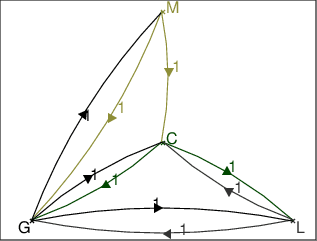
\includegraphics[width=\textwidth]{grapheprob}\end{center}
On tape :
\begin{center}{\tt  graphe\_probabiliste([[1/2,1/3,1/12,1/12],[1/3,1/2,1/6,0], 
[0,0,1/2,1/2],[1/4,1/4,1/4,1/4],
["Gare","Campus","Bibli","Centre"]])}\end{center}
On obtient :
\begin{center}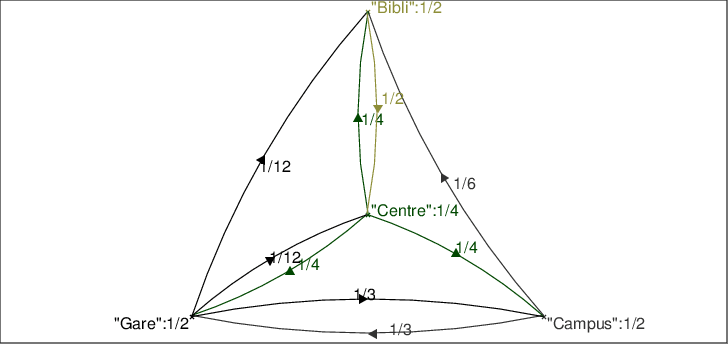
\includegraphics[width=\textwidth]{grapheprob1}\end{center}
On tape :
\begin{center}{\tt graphe\_probabiliste([[1/2,1/3,1/12,1/12],[1/3,1/2,1/6,0], 
[0,0,1/2,1/2],[1/4,1/4,1/4,1/4]],[0,1,i,1/2+2/3*i])}\end{center}
On obtient :
\begin{center}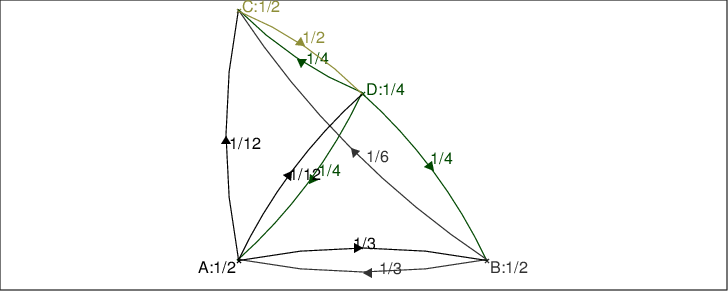
\includegraphics[width=\textwidth]{grapheprob2}\end{center}
On tape :
\begin{center}{\tt graphe\_probabiliste([[1/2,1/3,1/12,1/12],[1/3,1/2,1/6,0], 
[0,0,1/2,1/2],[1/4,1/4,1/4,1/4],
["Gare","Campus","Bibli","Centre"]], [0,1,i,1/2+2/3*i])}\end{center}
On obtient :
\begin{center}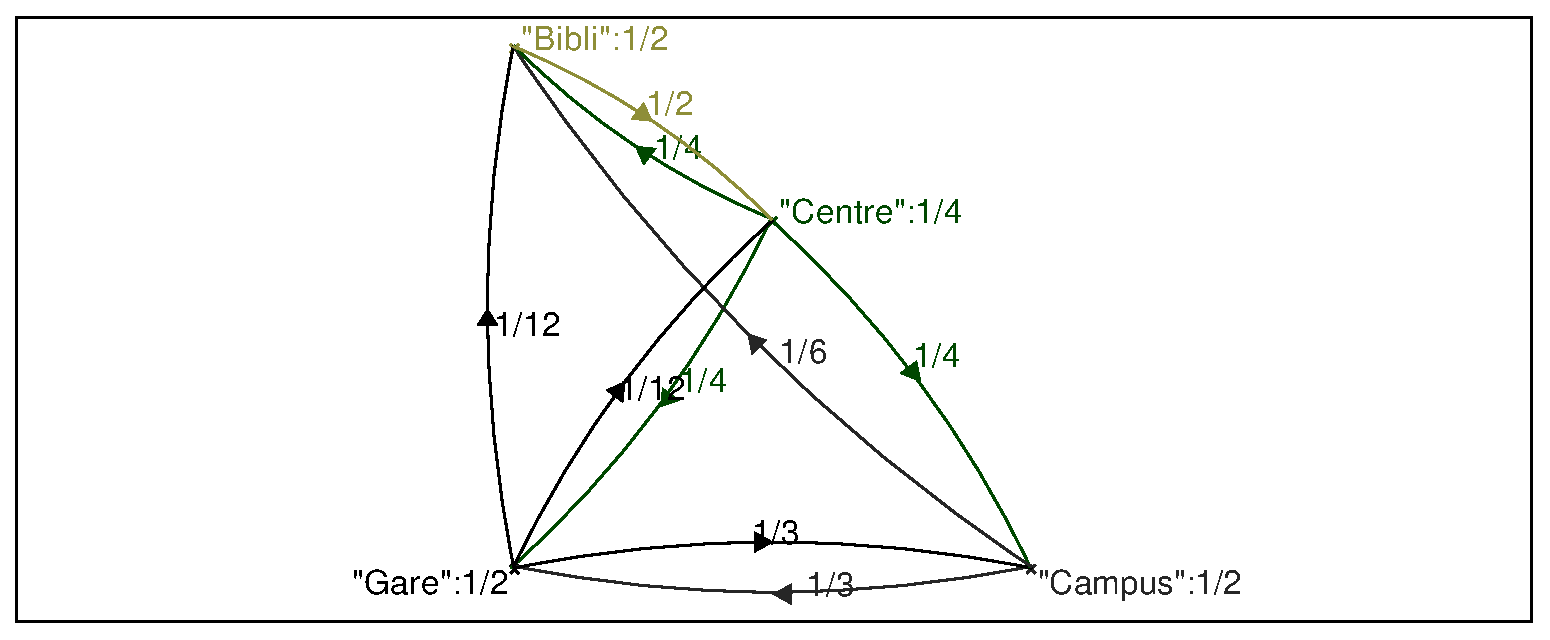
\includegraphics[width=\textwidth]{grapheprob3}\end{center}
Si on ne met pas les "" autour d'un nom, si ce nom est le nom d'une variable
qui contient une valeur c'est cette valeur que sera affich\'ee sinon les noms 
s'afficheront sans "". \\
On peut aussi d\'efinir les points pour d\'efinir le graphe, par exemple, 
on tape dans un nieau de g\'eom\'etrie 2d :\\ :\\
{\tt A:=point(0);}\\ 
{\tt B:=point(1);}\\ 
{\tt C:=point(i);}\\ 
{\tt D:=point(2/2+2i/3);}\\
{\tt graphe\_probabiliste([[1/2,1/3,1/12,1/12],[1/3,1/2,1/6,0], 
[0,0,1/2,1/2],[1/4,1/4,1/4,1/4]],[A,B,C,D])} \\
On peut alors bouger les points {\tt A,B,C,D} en mode pointeur.\\
On obtient apr\`es avoir boug\'e  {\tt D} :
\begin{center}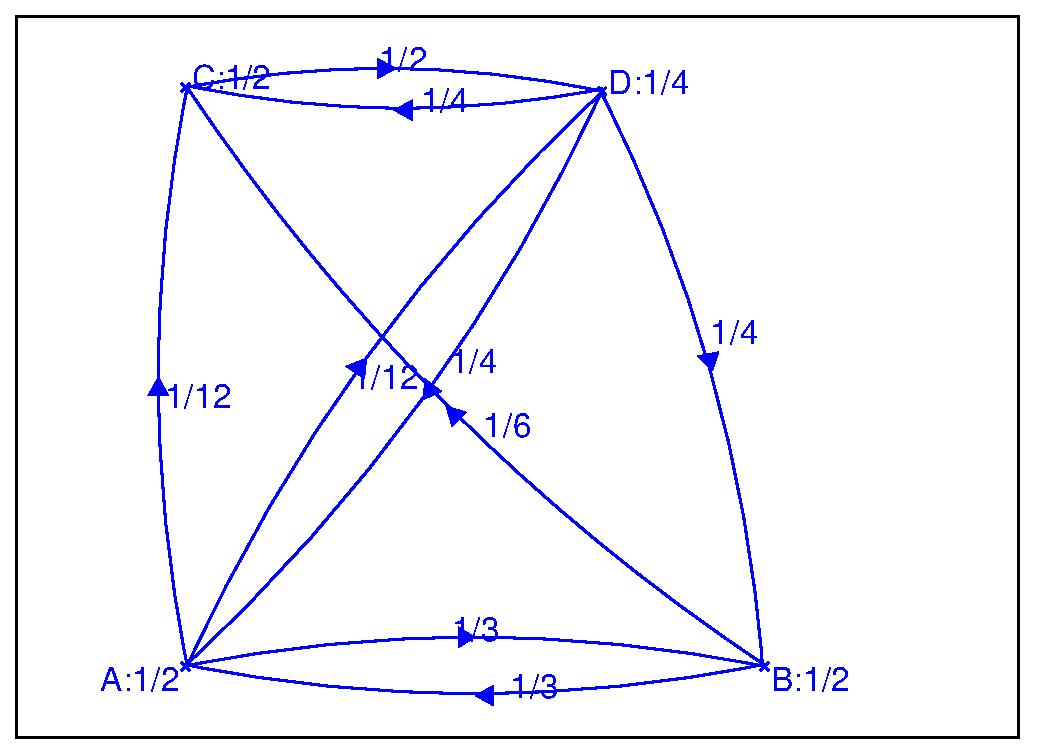
\includegraphics[width=7cm]{grapheproba4}\end{center}
\section{Graphe d'une fonction : {\tt plotfunc funcplot DrawFunc Graph}}\index{plotfunc|textbf}\index{funcplot|textbf}\index{DrawFunc|textbf}\index{Graph|textbf}\index{xstep@{\sl xstep}}\index{ystep@{\sl ystep}}\index{zstep@{\sl zstep}}\index{nstep@{\sl nstep}}
\subsection{Graphe en 2-d}\label{sec:plotfunc}
\noindent{\tt plotfunc(f(x),x)} trace la repr\'esentation graphique de 
$y=f(x)$ et \\
{\tt plotfunc(f(x),x=a..b)} trace la repr\'esentation graphique 
de $y=f(x)$ lorsque $a\leq x\leq b$.\\
On tape :
\begin{center}{\tt  plotfunc(x\verb|^|2-2)}\end{center}
ou
\begin{center}{\tt  plotfunc(a\verb|^|2-2,a=-1..2)}\end{center}
On obtient :
\begin{center}{\tt la repr\'esentation graphique de y=x\verb|^|2-2}\end{center}
On peut rajouter un param\`etre pour indiquer le saut 
d'\'echantillonnage en $x$ c'est \`a dire le pas en $x$ que l'on veut 
utiliser pour faire le graphe en utilisant \verb|xstep|.\\
On tape :
\begin{center}{\tt  plotfunc(x\verb|^|2-2,x,xstep=1)}\end{center}
On obtient :
\begin{center}{\tt une ligne polygonale qui est la repr\'esentation grossi\`ere de y=x\verb|^|2-2 }\end{center}
On peut aussi sp\'ecifier le nombre de points d'\'echantillonage de la
fonction \`a repr\'esenter en utilisant \verb|nstep| \`a la place de \verb|xstep|. 
Par exemple, on tape~:
\begin{center}{\tt  plotfunc(x\verb|^|2-2,x=-2..3,nstep=30)}\end{center}

\subsection{Graphe en 3-d}\label{sec:plotfunc3}
\noindent{\tt plotfunc} a deux arguments principaux et \'eventuellement
le saut d'\'echantillonnage des variables ({\tt xstep=} et {\tt ystep=}) c'est 
\`a dire le pas en $x$ et en $y$ que l'on choisi pour le graphe. On peut aussi 
sp\'ecifier le nombre de points d'\'echantillonnage de la fonction \`a repr\'esenter en
utilisant \verb|nstep|.\\
Les deux arguments principaux de {\tt plotfunc} sont : une expression de deux 
variables  ou une liste de plusieurs expressions de deux 
variables et la liste des deux variables.\\
{\tt plotfunc} trace la (ou les) surfaces d\'efinie par le premier argument.\\ 
On peut faire tourner ce graphique selon l'axe des {\tt x}, l'axe des {\tt y} 
ou l'axe des {\tt z}. Pour cela, il faut 
cliquer avec la souris dans la fen\^etre graphique en dehors du 
parall\'el\'epip\'ede servant \`a la repr\'esentation, puis faire bouger la 
souris  (sans relacher son bouton) ou  utiliser les  touches 
{\tt x}, {\tt X}, {\tt y}, {\tt Y}, {\tt z} et {\tt Z}.\\
%On tape sur {\tt OK} quand on est satisfait. \\
On tape :
\begin{center}{\tt plotfunc( x\verb|^|2+y\verb|^|2,[x,y])}\end{center}
On obtient :
\begin{center}{\tt Un graphique en 3-d repr\'esentant z=x\verb|^|2+y\verb|^|2}\end{center}
On tape :
\begin{center}{\tt plotfunc(x*y,[x,y]) }\end{center}
On obtient :
\begin{center}{La surface z=x*y}\end{center}
On tape :
\begin{center}{\tt plotfunc([x*y-10,x*y,x*y+10],[x,y]) }\end{center}
On obtient :
\begin{center}{Les surfaces z=x*y-10, z=x*y et z=x*y+10}\end{center}
Pour n'avoir qu'une portion de surface on peut indiquer l'intervalle de 
variation dans le deuxi\`eme et le trois\`eme argument.\\
On tape :
\begin{center}{\tt plotfunc(x*sin(y),[x=0..2,y=-pi..pi]) }\end{center}
On obtient :
\begin{center}{\tt Une portion de  surface $z=x*y$}\end{center}

On peut rajouter un param\`etre pour indiquer le saut 
d'\'echantillonnage en $x$ et en $y$ c'est \`a dire le pas en $x$ et en $y$ que
l'on veut utiliser pour faire le graphe, en utilisant\verb|xstep| et 
\verb|ystep|.\\ 
On tape :
\begin{center}{\tt plotfunc(x*sin(y),[x=0..2,y=-pi..pi],xstep=1,ystep=0.5) }\end{center}
On obtient :
\begin{center}{\tt Une portion de  surface $z=x*y$}\end{center}
On peut aussi sp\'ecifier le nombre de points d'\'echantillonage de la
fonction \`a repr\'esenter en utilisant \verb|nstep| \`a la place de \verb|xstep| et
\verb|ystep|. 
Par exemple, on tape~:
\begin{center}{\tt plotfunc(x*sin(y),[x=0..2,y=-pi..pi],nstep=300)}\end{center}
On obtient :
\begin{center}{\tt Une portion de  surface $z=x*y$}\end{center}
{\bf Remarque}\\
 Si vous voulez l'impression ou la traduction en Latex, il faut utiliser :\\
{\tt M$\blacktriangleright$Exporter/Imprimer$\blacktriangleright$Print(with Latex)}. 

\subsection{Graphe "3-d" avec les couleurs de l'arc en ciel}\label{sec:plotfunc3d}
\noindent{\tt plotfunc} permet aussi de repr\'esenter une expression {\tt Xpr}
d\'ependant de deux variables \`a valeur dans $\mathbb{R}$, en repr\'esentant
{\tt z=Xpr} par une couleur. Cela permet de visualiser les points ayant m\^eme
cote.\\
Les deux arguments principaux de {\tt plotfunc} sont alors {\tt i*Xpr} et la 
liste des noms de deux variables.\\
Pour n'avoir qu'une portion de surface on peut indiquer l'intervalle de 
variation dans le deuxi\`eme et le trois\`eme argument.\\
On peut rajouter un param\`etre pour indiquer le pas en $x$ et en $y$ que
l'on veut utiliser pour faire le graphe, en utilisant\verb|xstep| et 
\verb|ystep|.\\ 
On peut aussi sp\'ecifier le nombre de points d'\'echantillonage de la
fonction \`a repr\'esenter en utilisant \verb|nstep| \`a la place de \verb|xstep| et
\verb|ystep|. \\
On tape :
\begin{center}{\tt plotfunc(i*x*sin(y),[x=0..2,y=-pi..pi])}\end{center}
On obtient :
\begin{center}{\tt Une portion de surface $z=x*y$ avec les couleurs de l'arc en ciel}\end{center}

\subsection{Graphe en "4D"}\label{sec:plotfunc4}
\noindent{\tt plotfunc} permet aussi de repr\'esenter une expression {\tt Xpr}
\`a valeur dans $\mathbb{C}$ mais non imaginaire pur : on repr\'esente 
{\tt abs(Xpr)} selon $Oz$ et {\tt arg(Xpr)} par une couleur. Cela permet de 
visualiser les points ayant m\^eme argument.\\
Si l'expression {\tt Xpr} est imaginaire pur c'est {\tt Xpr/i} qui est 
represent\'e en d\'egrad\'e (cf \ref{sec:plotfunc3d})
Les deux arguments principaux de {\tt plotfunc} sont alors  une expression de 
deux variables \`a valeur dans  $\mathbb{C}$ et la liste des noms des deux 
variables.\\
On peut aussi sp\'ecifier le nombre de points d'\'echantillonnage de la
fonction \`a repr\'esenter en utilisant \verb|nstep| et demander un affichage en 
une forme pleine ({\tt affichage=rempli}).\\
{\tt plotfunc} trace la  surface aux couleurs de l'arc en ciel d\'efinie par le
module du premier argument soit {\tt z=abs(Xpr)}, chaque couleur est une 
valeur de {\tt arg(Xpr)}.\\ 
On peut faire tourner ce graphique selon 
l'axe des {\tt x}, l'axe des {\tt y} ou l'axe des {\tt z}. Pour cela, il faut 
cliquer avec la souris dans la fen\^etre graphique  en dehors du 
parall\'el\'epip\'ede servant \`a la repr\'esentation, puis faire bouger la 
souris  (sans relacher son bouton) ou utiliser les  touches {\tt x}, {\tt X}, 
{\tt y}, {\tt Y}, {\tt z} et {\tt Z}.\\
%On tape sur {\tt OK} quand on est satisfait. \\
On tape :
\begin{center}{\tt plotfunc((x+i*y)\verb|^|2,[x,y])}\end{center}
On obtient :
\begin{center}{\tt Un graphique en 3-d color\'e repr\'esentant z=abs((x+i*y)\verb|^|2 et permettant de visualiser les points ayant m\^eme argument}\end{center}
On tape :
\begin{center}{\tt plotfunc((x+i*y)\verb|^|2,[x,y],affichage=rempli)}\end{center}
On obtient :
\begin{center}{La surface pr\'ecedente selon une forme pleine aux couleurs de l'arc en ciel}\end{center}
Pour n'avoir qu'une portion de surface on peut indiquer l'intervalle de 
variation dans le deuxi\`eme et le trois\`eme argument.\\
On tape :
\begin{center}{\tt plotfunc((x+i*y)\verb|^|2,[x=-1..1,y=-2..2], nstep=900, affichage=rempli)}\end{center}
On obtient :
\begin{center}{La portion de la surface pr\'ecedente selon une forme pleine aux couleurs de l'arc en ciel avec x entre -1 et 1, y entre -2 et 2 et avec 900 points d'\'echantillonnage}\end{center}
{\bf Remarque}\\
 Si vous voulez l'impression ou la traduction en Latex, il faut utiliser :\\
{\tt M$\blacktriangleright$Exporter/Imprimer$\blacktriangleright$Print(with Latex)}. 

\section{Graphe 2-d pour compatibilit\'e Maple : {\tt plot graphe}}
\index{plot}\index{graphe} \label{sec:plot2d}
\noindent{\tt plot(f(x),x)} trace la repr\'esentation graphique de $y=f(x)$.\\
On tape :
\begin{center}{\tt  plot(x\verb|^|2-2,x)}\end{center}
On obtient :
\begin{center}{\tt la repr\'esentation graphique de y=x\verb|^|2-2}\end{center}
On peut rajouter un param\`etre pour indiquer le saut 
d'\'echantillonnage en $x$ c'est \`a dire le pas en x que l'on veut 
utiliser pour faire le graphe.
On tape :
\begin{center}{\tt  plot(x\verb|^|2-2,xstep=1)}\end{center}
ou encore
\begin{center}{\tt  plot(x\verb|^|2-2,x,xstep=1)}\end{center}
On obtient :
\begin{center}{\tt une ligne polygonale qui est la repr\'esentation grossi\`ere de y=x\verb|^|2-2}\end{center}
On peut aussi sp\'ecifier le nombre de points d'\'echantillonage de la
fonction \`a repr\'esenter en utilisant \verb|nstep| \`a la place
de \verb|xstep|. Par exemple, on tape~:
\begin{center}{\tt  plot(x\verb|^|2-2,x=-2..3,nstep=30)}\end{center}

\section{Surface 3-d pour compatibilit\'e Maple {\tt plot3d graphe3d}}\index{plot3d}\index{graphe3d}
\noindent{\tt plot3d} a trois arguments une fonction de deux variables (ou une 
expression de deux variables  ou une liste de trois fonctions de deux variables
ou encore une liste de trois expressions de deux variables) et les noms de ces
deux variables.\\
{\tt plot3d} trace la surface d\'efinie par le premier argument (soit $z=f(x,y)$, soit $x=f(u,v),y=g(u,v),z=h(u,v)$).\\ 
On peut faire tourner ce graphique selon 
l'axe des {\tt x}, l'axe des {\tt y} ou l'axe des {\tt z}. Pour cela, il faut 
cliquer avec la souris dans la fen\^etre graphique  en dehors du 
parall\'el\'epip\'ede servant \`a la repr\'esentation, puis faire bouger la 
souris  (sans relacher son bouton) ou utiliser les  touches {\tt x}, {\tt X}, 
{\tt y}, {\tt Y}, {\tt z} et {\tt Z}.\\
On tape :
\begin{center}{\tt plot3d(x*y,x,y)}\end{center}
On obtient :
\begin{center}{La surface $z=x*y$}\end{center}
On tape :
\begin{center}{\tt plot3d([v*cos(u),v*sin(u),v],u,v) }\end{center}
On obtient :
\begin{center}{Le c\^one $x=v*\cos(u),y=v*\sin(u),z=v$}\end{center}
Pour n'avoir qu'une portion de surface on peut indiquer l'intervalle de variation dans le deuxi\`eme et le trois\`eme argument.\\
On tape :
\begin{center}{\tt plot3d([v*cos(u),v*sin(u),v],u=0..pi,v=0..3)}\end{center}
On obtient :
\begin{center}{Une portion du c\^one $x=v*\cos(u),y=v*\sin(u),z=v$}\end{center}

\section{Graphe d'une droite et les tangentes \`a un graphe}
\subsection{Trac\'e d'une droite : {\tt line droite}}\index{line}\index{droite}\label{sec:droite}
{\bf Voir aussi :} \ref{sec:droite2} et \ref{sec:droite3} pour la droite en 
g\'eom\'etrie et \ref{sec:axe2} et \ref{sec:axe3} pour la droite orient\'ee.\\
\noindent {\tt droite} a comme argument son \'equation cart\'esienne :
\begin{itemize}
\item en 2-d \\
une \'equation de droite,
\item en 3-d \\
deux \'equations de plan.
\end{itemize}
 {\tt droite} d\'efinit et trace la droite d'\'equation donn\'ee en argument.\\
On tape :
\begin{center}{\tt droite(2*y+x-1=0)}\end{center}
On obtient :
\begin{center}{\tt le trac\'e de la droite 2*y+x-1=0}\end{center}
On tape : 
\begin{center}{\tt droite(y=1)}\end{center}
On obtient :
\begin{center}{\tt le trac\'e de la droite horizontale y=1}\end{center}
On tape :
\begin{center}{\tt droite(x=1)}\end{center}
On obtient :
\begin{center}{\tt le trac\'e de la droite verticale x=1}\end{center}
On tape :
\begin{center}{\tt droite(x+2*y+z-1=0,z=2)}\end{center}
On obtient :
\begin{center}{\tt le trac\'e de la droite x+2*y+1=0 dans le plan z=2}\end{center}
On tape :
\begin{center}{\tt droite(y=1,x=1)}\end{center}
On obtient :
\begin{center}{\tt le trac\'e de la droite verticale passant par (1,1,0)}\end{center}
{\bf Remarque}\\
{\tt droite} d\'efinit une droite orient\'ee :
\begin{itemize}
\item Lorsque la droite 2-d est donn\'ee par son \'equation, on met cette 
\'equation sous la forme "membre\_gauche-membre\_droite={\tt ax+by+c=0}", cela 
d\'etermine son vecteur normal {\tt [a,b]} et l'orientation est donn\'ee par le 
vecteur {\tt [b,-a]}) (ou encore son orientation est d\'efinie par le produit 
vectoriel 3-d de son vecteur normal (de cote 0) et du vecteur de coordonn\'ees 
[0,0,1]).\\
Par exemple {\tt droite(y=2*x)} d\'efinit une droite orient\'ee par le vecteur 
 de coordonn\'ees {\tt [1,2]}.
\item Lorsque la droite 3-d est donn\'ee par deux \'equations de plans, son 
orientation est d\'efinie par le produit vectoriel des normales aux plans (en 
mettant les \'equations des plans sous la forme 
"membre\_gauche-membre\_droite=0" on  d\'etermine les normales orient\'ees de 
ces plans).\\
Par exemple, {\tt droite(x=y,y=z)} est orient\'ee par :\\ 
{\tt cross([1,-1,0],[0,1,-1])}={\tt [1,1,1]}.
\end{itemize}

\subsection{Trac\'e d'une droite horizontale en 2-d : {\tt LineHorz}}\index{LineHorz}
\noindent {\tt LineHorz} a comme argument une expression $Xpr$.\\
 {\tt LineHorz} trace la droite horizontale $y=Xpr$.\\
On tape :
\begin{center}{\tt LineHorz(1)}\end{center}
On obtient :
\begin{center}{\tt le trac\'e de la droite y=1}\end{center}

\subsection{Trac\'e d'une droite verticale en 2-d : {\tt LineVert}}\index{LineVert}
\noindent {\tt LineVert} a  comme arguments une expression $Xpr$.\\
 {\tt LineVert} trace la la droite verticale $x=Xpr$.\\
On tape :
\begin{center}{\tt LineVert(1)}\end{center}
On obtient :
\begin{center}{\tt le trac\'e de la droite x=1}\end{center}

\subsection{Tangente \`a un graphe en 2-d : {\tt LineTan droite\_tangente}}\index{LineTan}\index{droite\_tangente}
\noindent {\tt LineTan} (resp {\tt droite\_tangente}) a deux arguments : une 
expression $Xpr$ de la variable $x$ et une valeur $x0$ de $x$.\\ 
{\bf Attention} pour {\tt LineTan} il ne faut pas mettre de parenth\`eses ou 
alors il faut les mettre \`a l'ext\'erieur.\\
 {\tt LineTan} (resp {\tt droite\_tangente}) trace la tangente en $x=x0$ \`a la
 repr\'esentation graphique
de $y=Xpr$.\\
On tape :
\begin{center}{\tt (LineTan ln(x),1)}\end{center}
Ou on tape :
\begin{center}{\tt droite\_tangente(ln(x),1)}\end{center}
On obtient :
\begin{center}{\tt le trac\'e de la droite y=x-1}\end{center}
On tape :
\begin{center}{\tt equation(LineTan ln(x),1)}\end{center}
Ou on tape :
\begin{center}{\tt equation(droite\_tangente(ln(x),1))}\end{center}
On obtient :
\begin{center}{\tt l'\'equation y=(x-1)}\end{center})

\subsection{Tangente en un point d'un graphe en 2-d : {\tt tangent tangente}}\index{tangent|textbf}\index{tangente|textbf}\label{sec:tangente}
{\bf Voir aussi :} \ref{sec:tangent} pour la g\'eom\'etrie plane et 
\ref{sec:tangent3} pour la g\'eom\'etrie 3-d.\\
\noindent {\tt tangent} a deux arguments : un objet g\'eom\'etrique et un 
point {\tt A}.\\
Mais quand l'objet g\'eom\'etrique est le graphe {\tt G} d'une fonction 2-d, 
le deuxi\`eme argument doit \^etre soit, un nombre r\'eel ${\tt x_0}$, soit un 
point {\tt A} situ\'e sur {\tt G}.\\

Par exemple on tape :\\
{\tt G:=plotfunc(g(x),x)}\\
{\tt tangent(G, 1.2)}\\
 trace la tangente au graphe {\tt G} de la fonction {\tt g} au point 
d'abscisse {\tt x=1.2},\\ 
ou on tape :\\
{\tt A:=point(1.2+i*g(1.2))}\\
{\tt tangent(G, A)}\\
trace la tangente au point {\tt A} du graphe {\tt G} de la fonction {\tt g}.\\
Par exemple, pour avoir le trac\'e de la tangente au graphe de $g(x)=x^2$ au 
point d'abscisse $x_0=1$, on tape :
\begin{center}{\tt g(x):=x\verb|^|2; G:=plotfunc(g(x),x)}\end{center}
\begin{center}{\tt T:=tangent(G,1)}\end{center}
ou on tape :
\begin{center}{\tt T:=tangent(G,point(1+i))}\end{center}
On obtient  
\begin{center}{\tt La tangente au graphe de $g(x)=x^2$ au point 1+i}\end{center}
L'\'equation de la tangente est alors obtenue en tapant :
\begin{center}{\tt equation(T)}\end{center}
\subsection{Trac\'e d'une droite donn\'ee par un point et sa pente : {\tt DrawSlp}}\index{DrawSlp}
\noindent {\tt DrawSlp} a comme argument trois r\'eels {\tt a,b,m}.\\
 {\tt DrawSlp} renvoie et trace la droite de pente {\tt m} et passant par le 
point de coordonn\'ees {\tt a,b}.\\
On tape :
\begin{center}{\tt DrawSlp(2,1,-1)}\end{center}
On obtient :
\begin{center}{\tt la droite d'\'equation y=(-x+3) qui a pour pente -1 et qui passe par le point(2,1)}\end{center}



\subsection{Intersection d'un graphe en 2-d  avec les axes}\index{solve}\index{resoudre}
Pour avoir l'ordonn\'ee de l'intersection du graphe de $f$ avec l'axe des 
$y$ on tape :
\begin{center}{\tt f(0)}\end{center}
le point de coordonn\'ees : $(0,f(0))$ est donc le point d'intersection du 
graphe de $f$ avec l'axe des $y$.\\
Pour avoir l'intersection du graphe de $f$ avec l'axe des $x$ il faut
r\'esoudre $f(x)=0$. On peut essayer d'avoir les valeurs exactes des 
abscisses de ces points en tapant :
\begin{center}{\tt solve(f(x),x)}\end{center}
ou avoir les valeurs approch\'ees de ces abscisses en utilisant la 
repr\'esentation graphique puis, en utilisant {\tt fsolve} pour avoir une 
meilleure pr\'ecision.

\section{Repr\'esentation graphique d'in\'equations \`a 2 variables : {\tt plotinequation inequationplot}}\index{plotinequation|textbf}\index{inequationplot|textbf}
\noindent{\tt plotinequation([f1(x,y)<a1,..,fk(x,y)<ak],[x=x1..x2,y=y1..y2])}
trace la surface du plan d\'efinie par les in\'equations \`a 2 variables :
$$f1(x,y)<a1$$
$$...$$
$$fk(x,y)<ak$$
$$ x1<x<x2$$
$$ y1<y<y2$$
On tape :
\begin{center}{\tt plotinequation(x\verb|^|2-y\verb|^|2<3, [x=-2..2,y=-2..2],xstep=0.1,ystep=0.1)}\end{center}
On obtient :
\begin{center}{\tt la partie contenant l'origine et d\'elimit\'ee par l'hyperbole x\verb|^|2-y\verb|^|2=3 est remplie}\end{center}
On tape :
\begin{center}{\tt plotinequation([x+y>3,x\verb|^|2<y], [x-2..2,y=-1..10],xstep=0.2,ystep=0.2)}\end{center}
On obtient :
\begin{center}{\tt le morceau du plan d\'efinit par -2<x<2,y<10,x+y>3,y>x\verb|^|2 est rempli}\end{center}
{\bf Attention}\\
Si on ne met pas les bornes pour $x$ et $y$ ce sont les valeurs de 
{\tt X-,X+,Y-,Y+} mises dans la configuration g\'en\'erale du graphique 
({\tt Cfg$\blacktriangleright$Configuration graphique}) qui
seront prises en compte.

\subsection{Aire  sous une courbe : {\tt area aire}}\index{aire|textbf}\index{area|textbf}\index{rectangle\_droit@{\sl rectangle\_droit}|textbf}\index{rectangle\_gauche@{\sl rectangle\_gauche}|textbf}\index{trapeze@{\sl trapeze}|textbf}\index{point\_milieu@{\sl point\_milieu}|textbf}\index{trapezoid@{\sl trapezoid}|textbf}\index{right\_rectangle@{\sl right\_rectangle}|textbf}\index{left\_rectangle@{\sl left\_rectangle}|textbf}\index{middle\_point@{\sl middle\_point}|textbf}
\index{simpson@{\sl simpson}|textbf}\index{rombergt@{\sl rombergt}|textbf}\index{rombergm@{\sl rombergm}|textbf}\index{rombergm@{\sl gauss15}|textbf}
\noindent {\tt aire} ou {\tt area} calcule de fa\c{c}on approch\'ee l'aire 
sous la courbe $y=f(x)$ comprise entre $x=a$ et $x=b$.\\
{\tt aire} ou {\tt area} a quatre arguments: l'expression $f(x)$, $x=a..b$,
un entier $n$ et le nom de la m\'ethode num\'erique choisie pour faire calcul.\\
La m\'ethode num\'erique est choisie parmi :\\
{\tt trapezoid, left\_rectangle, right\_rectangle, middle\_point} ou
{\tt trapeze, rectangle\_gauche, rectangle\_droit, point\_milieu} et aussi
{\tt simpson} (m\'ethode de Simpson), {\tt rombergt} (acc\'el\'eration de 
convergence de Romberg avec la m\'ethode des trap\`ezes), {\tt rombergm} 
(acc\'el\'eration de convergence de Romberg avec la m\'ethode du point milieu) 
et {\tt gauss15} (avec une quadrature de Gauss adaptative \`a 15 points).\\
La valeur de l'entier $n$ est le nombre de subdivisions que l'on a choisi pour 
les calculs faits avec les m\'ethodes {\tt trapezoid, left\_rectangle, 
right\_rectangle, middle\_point} ou {\tt trapeze, rectangle\_gauche, 
rectangle\_droit, point\_milieu, simpson} alors que pour {\tt gauss15}, 
{\tt rombergt} et {\tt rombergm} le nombre de subdivisions est $2^n$.\\
 Ainsi,{\tt area(f(x),x=a..b,n,trapeze)} calcule l'aire de $n$ trap\`ezes : \\
le troisi\`eme argument est un entier $n$, et le
quatri\`eme argument est le nom de la m\'ethode num\'erique d'int\'egration 
lorsqu'on partage $[a,b]$ en $n$ parties \'egales.\\
{\tt area(f(x),x=a..b,n,rombergt)} revient \`a calculer l'aire de $2^n$ 
trap\`ezes qui sont acc\'el\'er\'es.\\ 
On tape :
\begin{center}{\tt area(x\verb|^|2,x=0..1,8,trapeze)}\end{center}
On obtient :
\begin{center}{\tt 0.3359375}\end{center}
On tape :
\begin{center}{\tt area(x\verb|^|2,x=0..1,8,point\_milieu)}\end{center}
On obtient :
\begin{center}{\tt 0.33203125}\end{center}
Donc comme $f(x)=x^2$ est convexe on a l'aire est dans l'intervalle :\\
$]0.33203125, 0.3359375[$:\\
On tape :
\begin{center}{\tt area(x\verb|^|2,x=0..1,3,rombergt)}\end{center}
On obtient une meilleur approximation :
\begin{center}{\tt 0.333333333333}\end{center}
On tape :
\begin{center}{\tt area(x\verb|^|2,x=0..1,3,rombergm)}\end{center}
On obtient une meilleur approximation :
\begin{center}{\tt 0.333333333333}\end{center}
On tape :
\begin{center}{\tt area(x\verb|^|2,x=0..1,3,gauss15)}\end{center}
On obtient :
\begin{center}{\tt 1/3}\end{center}
On tape :
\begin{center}{\tt area(x\verb|^|2,x=0..1)}\end{center}
On obtient :
\begin{center}{\tt 1/3}\end{center}

\section{Repr\'esentation graphique de l'aire sous une courbe : {\tt tracer\_aire graphe\_aire aire\_graphe plotarea areaplot}}\index{tracer\_aire|textbf}\index{graphe\_aire|textbf}\index{aire\_graphe|textbf}\index{plotarea|textbf}\index{areaplot|textbf}\index{rectangle\_droit@{\sl rectangle\_droit}|textbf}\index{rectangle\_gauche@{\sl rectangle\_gauche}|textbf}\index{trapeze@{\sl trapeze}|textbf}\index{point\_milieu@{\sl point\_milieu}|textbf}\index{trapezoid@{\sl trapezoid}|textbf}\index{right\_rectangle@{\sl right\_rectangle}|textbf}\index{left\_rectangle@{\sl left\_rectangle}|textbf}\index{middle\_point@{\sl middle\_point}|textbf}
\begin{itemize}
\item  Avec deux arguments, {\tt aire\_graphe} ou {\tt plotarea} permet 
de repr\'esenter et d'afficher avec 3 digits l'aire sous une courbe.\\
Ainsi, {\tt plotarea(f(x),x=a..b)} trace l'aire sous 
la courbe $y=f(x)$ pour $a<x<b$, c'est \`a dire la portion du plan d\'efinie 
par les in\'equations $a<x<b$ et selon le signe de 
$f(x)$ $0<y<f(x)$ ou $0>y>f(x)$.\\
On tape :
\begin{center}{\tt plotarea(sin(x),x=0..2*pi)}\end{center}
On obtient :
\begin{center}{\tt la portion de plan situ\'e dans les deux arches de sin(x)}\end{center}

\item Avec quatre arguments, {\tt aire\_graphe} ou {\tt plotarea} permet 
de repr\'esenter l'aire qui est cacul\'ee avec la m\'ethode num\'erique choisie
 parmi :\\
{\tt trapezoid, left\_rectangle, right\_rectangle, middle\_point} ou
{\tt trapeze, rectangle\_gauche, rectangle\_droit, point\_milieu}.\\
 Ainsi, {\tt plotarea(f(x),x=a..b,n,trapeze)} trace l'aire
de $n$ trap\`ezes : le troisi\`eme argument est un entier $n$, et le
quatri\`eme argument est le nom de la m\'ethode num\'erique d'int\'egration 
lorsqu'on partage $[a,b]$ en $n$ parties \'egales.\\
On tape :
\begin{center}{\tt plotarea(x\verb|^|2,x=0..1,5,trapeze)}\end{center}
Ou on tape pour voir la courbe en rouge :
\begin{center}{\tt plotarea(x\verb|^|2,x=0..1,5,trapeze); plot(x\verb|^|2,x=0..1,affichage=rouge)}\end{center}
On obtient :
\begin{center}{\tt les 5 trap\`ezes qui sont utilis\'es dans la m\'ethode dite des trap\`ezes, pour approcher une int\'egrale}\end{center}
On tape :
\begin{center}{\tt plotarea(x\verb|^|2,x=0..1,5,point\_milieu)}\end{center}
Ou on tape pour voir la courbe en rouge :
\begin{center}{\tt plotarea(x\verb|^|2,x=0..1,5,point\_milieu); plot(x\verb|^|2,x=0..1,affichage=rouge)}\end{center}
On obtient :
\begin{center}{\tt les 5 rectangles qui sont utilis\'es dans la m\'ethode dite du point milieu, pour approcher une int\'egrale}\end{center}
\end{itemize}
{\bf Remarque 1} On peut aussi taper, pour n'avoir que la valeur de l'aire :
\begin{center}{\tt plotarea(x\verb|^|2,x=0..1,5,trapeze)[0,3];}\end{center}
On obtient :
\begin{center}{\tt 0.34}\end{center}
{\bf Remarque 2} Si on utilise {\tt plotarea} avec le menu 
{\tt Graphic->Courbes->plotarea} une boite de dialogue s'ouvre : vous entrez,
l'expression de la fonction, le nom de la variable, les bornes de l'intervalle
{\tt xmin,xmax}, le pas  {\tt xstep} (on a alors {\tt n=(xmax-xmin)/xstep}),
la m\'ethode d'int\'egration et aussi la couleur du dessin (on retrouve en 
effet le bouton {\tt Attribut} en haut et \`a gauche de la boite de dialogue).

\section{Lignes de niveaux : {\tt plotcontour contourplot \\DrwCtour}}\index{plotcontour|textbf}\index{contourplot|textbf}\index{DrwCtour|textbf}\label{sec:plotcontour}
\noindent{\tt plotcontour(f(x,y),[x,y])} (ou {\tt DrwCtour(f(x,y),[x,y])} ou \\
encore {\tt contourplot(f(x,y),[x,y])})
trace les 11 lignes de niveaux $z=-10$, $z=-8$,.., $z=0$, $z=2$,.., $z=10$ de la
surface d\'efinie par $z=f(x,y)$.\\
On tape :
\begin{center}{\tt plotcontour(x\verb|^|2+y\verb|^|2,[x=-3..3,y=-3..3],[1,2,3], affichage=[vert,rouge,noir]+[rempli\$3])}\end{center}
On obtient :  
\begin{center}{\tt  le graphe des trois cercles x\verb|^|2+y\verb|^|2=n pour n=1,2,3; les zones comprises entre ces cercles sont remplies avec la couleur verte,rouge ou noire }\end{center}
On tape :
\begin{center}{\tt  plotcontour(x\verb|^|2-y\verb|^|2,[x,y])}\end{center}
On obtient :
\begin{center}{\tt  le graphe des 11 hyperboles x\verb|^|2-y\verb|^|2=n pour n=-10,-8,..10}\end{center}

Pour visualiser la surface, on tape ({\tt plotfunc(f(x,y),[x,y])} trace la 
repr\'esentation graphique de $z=f(x,y)$, voir \ref{sec:plotfunc3}):
\begin{center}{\tt plotfunc( x\verb|^|2-y\verb|^|2,[x,y])}\end{center}
On obtient :
\begin{center}{\tt Un graphique en 3-d repr\'esentant z=x\verb|^|2+y\verb|^|2}\end{center}
On peut faire tourner ce graphique selon l'axe des {\tt x}, l'axe des {\tt y} 
ou l'axe des {\tt z}. Pour cela, il faut 
cliquer avec la souris dans la fen\^etre graphique  en dehors du 
parall\'el\'epip\'ede servant \`a la repr\'esentation, puis faire bouger la 
souris (sans relacher son bouton) ou utiliser aux touches 
{\tt x}, {\tt X}, {\tt y}, {\tt Y}, {\tt z} et {\tt Z}.

\section{Graphe d'une fonction par niveaux de couleurs : {\tt plotdensity densityplot}}\index{plotdensity|textbf}\index{densityplot|textbf}
\noindent{\tt plotdensity(f(x,y),[x,y])}  ou 
encore {\tt densityplot(f(x,y),[x,y])}
trace le graphe de $z=f(x,y)$ dans le plan en repr\'esentant
$z$ par une des couleurs de l'arc en ciel.\\
On tape :
\begin{center}{\tt  plotdensity(x\verb|^|2-y\verb|^|2,[x=-2..2,y=-2..2],xstep=0.1,ystep=0.1)}\end{center}
On obtient :
\begin{center}{\tt Un graphique en 2-d repr\'esentant pour chaque z, l'hyperbole d\'efinie par x\verb|^|2-y\verb|^|2=z par une couleur de l'arc en ciel}\end{center}
On remarquera que l'on a l'echelle des couleurs en dessous du graphe.

\section{Courbe implicite : {\tt plotimplicit implicitplot}}\index{plotimplicit|textbf}\index{implicitplot|textbf}\index{unfactored|textbf}\index{sans\_factoriser|textbf} 
\noindent {\tt plotimplicit} ou {\tt implicitplot} permet de tracer des courbes ou des 
surfaces d\'efinies de façon implicite par une expression. 
Pour que {\tt Xcas} ne cherche pas \`a  factoriser l'expression, la commande 
{\tt plotimplicit} ou {\tt implicitplot} peut \^etre utilis\'ee avec l'option 
{\tt unfactored} ou {\tt sans\_factoriser} mise comme dernier param\`etre, : 
\begin{itemize}
\item avec {\tt unfactored} l'expression ne sera pas modifi\'ee,
\item sans {\tt unfactored} {\tt Xcas}  r\'eduit l'expression au m\^eme 
d\'enominateur puis cherche \`a  factoriser le num\'erateur. 
\end{itemize}

\subsection{Courbe implicite en 2-d}\label{sec:implicitplot}
\begin{itemize}
\item {\tt plotimplicit(f(x,y),x,y)} ou {\tt plotimplicit(f(x,y),[x,y])} trace 
la repr\'esentation graphique
de la courbe d\'efinie implicitement par $f(x,y)=0$ lorsque $x$ (resp $y$) 
varie selon {\tt WX-, WX+} (resp  {\tt WY-, WY+}) d\'efini dans {\tt cfg},
\item {\tt plotimplicit(f(x,y),x=0..1,y=-1..1)} ou \\
{\tt plotimplicit(f(x,y),[x=0..1,y=-1..1])} trace la repr\'esentation 
graphique de la courbe d\'efinie implicitement par $f(x,y)=0$ lorsque 
$0\leq x \leq 1$ et $-1\leq y \leq 1$ (mettre des bornes un peu plus grandes 
pour ne pas avoir de manques !).\\ 
\end{itemize}
On peut \'eventuellement rajouter encore deux param\`etres pour sp\'ecifier
le saut d'\'echantillonnage des variables avec {\tt xstep=} et {\tt ystep=}, 
c'est \`a dire le pas en $x$ et en $y$ que l'on choisi pour le graphe.\\
On tape :
\begin{center}{\tt plotimplicit(x\verb|^|2+y\verb|^|2-1,[x,y])}\end{center}
Ou on tape :
\begin{center}{\tt plotimplicit(x\verb|^|2+y\verb|^|2-1,x,y,unfactored)}\end{center}
On obtient :
\begin{center}{\tt Le dessin du cercle unit\'e}\end{center}
On tape :
\begin{center}{\tt plotimplicit(x\verb|^|2+y\verb|^|2-1,x,y,xstep=0.2,ystep=0.3)}\end{center}
Ou on tape :
\begin{center}{\tt plotimplicit(x\verb|^|2+y\verb|^|2-1,[x,y],xstep=0.2,ystep=0.3)}\end{center}
Ou on tape :
\begin{center}{\tt plotimplicit(x\verb|^|2+y\verb|^|2-1,[x,y], xstep=0.2,ystep=0.3,unfactored)}\end{center}
On obtient :
\begin{center}{\tt Le dessin du cercle unit\'e}\end{center}
On tape :
\begin{center}{\tt plotimplicit(x\verb|^|4+y\verb|^|4=x\verb|^|2+y\verb|^|2)}\end{center}
On obtient :
\begin{center}{\tt Le dessin du symbole infini}\end{center}
On tape :
\begin{center}{\tt plotimplicit(x\verb|^|2+4*y\verb|^|3-k)\$(k=1..5)}\end{center}
On obtient :
\begin{center}{\tt Le dessin de 5 courbes de la forme du chapeau de Napol\'eon}\end{center}

\subsection{Surface implicite en 3-d}\label{sec:implicitplot3}
\begin{itemize}
\item {\tt plotimplicit(f(x,y,z),x,y,z)} trace la repr\'esentation graphique
de la surface d\'efinie implicitement par : $f(x,y,z)=0$,
\item {\tt plotimplicit(f(x,y,z),x=0..1,y=-1..1,z=-1..1)} trace la 
repr\'esentation graphique de la surface d\'efinie implicitement par 
$f(x,y,z)=0$ lorsque $0\leq x \leq 1$, $-1\leq y \leq 1$ et $-1\leq z \leq 1$.
\end{itemize}
On peut \'eventuellement rajouter trois param\`etres pour sp\'ecifier
le saut d'\'echantillonnage des variables ({\tt xstep=}, {\tt ystep=} et 
{\tt zstep=}) c'est \`a dire le pas en $x$, en $y$ et en $z$ que l'on choisi 
pour le graphe.\\
On tape :
\begin{center}{\tt plotimplicit(x\verb|^|2+y\verb|^|2+z\verb|^|2-1,x,y,z, xstep=0.2,ystep=0.1,zstep=0.3)}\end{center}
On tape :
\begin{center}{\tt plotimplicit(x\verb|^|2+y\verb|^|2+z\verb|^|2-1,x,y,z, xstep=0.2,ystep=0.1,zstep=0.3,unfactored)}\end{center}
On obtient :
\begin{center}{\tt Le dessin de la sph\`ere unit\'e}\end{center}
On tape :
\begin{center}{\tt plotimplicit(x\verb|^|2+y\verb|^|2+z\verb|^|2-1,x=-1..1,y=-1..1,z=-1..1)}\end{center}
On obtient :
\begin{center}{\tt Le dessin de la sph\`ere unit\'e}\end{center}
\section{Courbe et surface en param\'etrique : {\tt plotparam paramplot DrawParm courbe\_parametrique}}\index{plotparam|textbf}\index{paramplot|textbf}\index{DrawParm|textbf}\index{courbe\_parametrique|textbf}
\subsection{Courbe 2-d en param\'etrique}
\noindent{\tt plotparam(f(t)+i*g(t),t)} 
(resp {\tt plotparam(f(t)+i*g(t),t=t1..t2)})
trace la repr\'esentation param\'etrique de la courbe d\'efinie par 
$x=f(t),y=g(t)$ (resp par  $x=f(t),y=g(t)$ et $t1 \geq t\geq t2$).\\
Si on ne pr\'ecise pas les bornes de l'intervalle de variation du param\`etre
ce sont les valeurs de {\tt t-} et {\tt t+} (cf \ref{sec:configgeo}) qui 
seront ces bornes.\\ 
On tape :
\begin{center}{\tt plotparam(cos(x)+i*sin(x),x) }\end{center}
ou 
\begin{center}{\tt plotparam([cos(x),sin(x)],x) }\end{center}
On obtient :
\begin{center}{\tt Le dessin du cercle unit\'e}\end{center}
On peut p\'eciser les bornes de l'intervalle de 
variation du param\`etre.\\ 
On tape si dans la configuration du graphique {\tt t} va de -4 \`a 1 :
\begin{center}{\tt plotparam(sin(t)+i*cos(t))}\end{center}
ou encore :
\begin{center}{\tt plotparam(sin(t)+i*cos(t),t=-4..1) }\end{center}
ou encore :
\begin{center}{\tt plotparam(sin(x)+i*cos(x),x=-4..1) }\end{center}
On obtient :
\begin{center}{\tt Le dessin de l'arc du cercle unit\'e allant de -4 \`a 1}\end{center}
On peut rajouter un param\`etre pour indiquer le saut d'\'echantillonnage du 
param\`etre $t$ avec {\tt tstep=} c'est \`a dire le pas en $t$ que l'on 
veut utiliser pour faire le graphe.\\
On tape si dans la configuration du graphique {\tt t} va de -4 \`a 1 :
\begin{center}{\tt plotparam(sin(t)+i*cos(t),t,tstep=0.5)}\end{center}
Ou on tape :
\begin{center}{\tt plotparam(sin(t)+i*cos(t),t=-4..1,tstep=0.5)}\end{center}
On obtient :
\begin{center}{Le dessin grossier de l'arc du cercle unit\'e allant de -4 \`a 1}\end{center}

\subsection{Surface 3-d en param\'etrique : {\tt plotparam paramplot DrawParm courbe\_parametrique}}\index{plotparam}\index{paramplot}\index{DrawParm}\index{courbe\_parametrique}
\noindent{\tt plotparam} a deux arguments principaux et \'eventuellement
les sauts d'\'echantillonnage des variables avec {\tt ustep=} et {\tt vstep=}, 
c'est \`a dire le pas en $u$ et en $v$ que l'on choisi pour le graphe.\\
Les deux arguments principaux de {\tt plotparam} sont : une liste de trois 
expressions de deux variables et la liste des deux variables.\\
{\tt plotparam([f(u,v),g(u,v),h(u,v)],[u,v])} trace la surface d\'efinie par le
premier argument soit $x=f(u,v),y=g(u,v),z=h(u,v)$).\\
On peut faire tourner ce graphique selon 
l'axe des {\tt x}, l'axe des {\tt y} ou l'axe des {\tt z}. Pour cela, il faut 
cliquer avec la souris dans la fen\^etre graphique  en dehors du 
parall\'el\'epip\'ede servant \`a la repr\'esentation, puis faire bouger la 
souris  (sans relacher son bouton) ou utiliser les  touches {\tt x}, {\tt X}, 
{\tt y}, {\tt Y}, {\tt z} et {\tt Z}.\\
On tape :
\begin{center}{\tt plotparam([v*cos(u),v*sin(u),v],[u,v]) }\end{center}
On obtient :
\begin{center}{\tt Le c\^one $x=v*\cos(u),y=v*\sin(u),z=v$}\end{center}
Pour n'avoir qu'une portion de surface on peut indiquer l'intervalle de 
variation dans le deuxi\`eme et le trois\`eme argument.\\
On tape :
\begin{center}{\tt plotparam([v*cos(u),v*sin(u),v],[u=0..pi,v=0..3]) }\end{center}
On obtient :
\begin{center}{\tt Une portion du c\^one $x=v*\cos(u),y=v*\sin(u),z=v$}\end{center}
On tape :
\begin{center}{\tt plotparam([v*cos(u),v*sin(u),v],[u=0..pi,v=0..3], ustep=0.5,vstep=0.5)}\end{center}
On obtient :
\begin{center}{\tt Une portion du c\^one $x=v*\cos(u),y=v*\sin(u),z=v$}\end{center}
{\bf Remarque}\\
 Si vous voulez l'impression ou la traduction en Latex, il faut utiliser :\\
{\tt M$\blacktriangleright$Exporter/Imprimer$\blacktriangleright$Print(with Latex)}. 
\section{Courbes de B\'ezier : {\tt bezier}}\index{bezier}
Soient $n+1$ points $P_j$ de contr\^ole ($j=0..n$) et $L$ la s\'equence de ces
 points.\\
La courbe de B\'ezier ayant les points de la s\'equence {\tt L} comme points de
contr\^ole, a comme \'equation param\'etrique :\\
$\sum_{j=0}^n comb(n,j)t^j(1-t)^{n-j}*L[j]$.\\
{\tt bezier(L,plot)} renvoie le trac\'e de la courbe d'\'equation 
param\'etrique : $\sum_{j=0}^n comb(n,j)t^j(1-t)^{n-j}*L[j]$.\\
{\tt parameq(bezier(L))} renvoie l'\'equation param\'etrique de la courbe de
 B\'ezier ayant comme points de contr\^ole les points de la s\'equence {\tt L}.\\
On tape :
\begin{center}{\tt bezier(1,1+i,2+i,3-i,plot)}\end{center}
On obtient :
\begin{center}{\tt Le trac\'e de la courbe de B\'ezier ayant comme points de contr\^ole les points d'affixe 1,1+i,2+i,3-i}\end{center}
On tape :
\begin{center}{\tt parameq(bezier(1,1+i,2+i,3-i))}\end{center}
On obtient :
\begin{center}{\tt L'\'equation param\'etrique de la courbe pr\'ec\'edente}\end{center}
On tape :
\begin{center}{\tt bezier(point([0,0,0]),point([1,1,0]),point([0,1,1]),plot)}\end{center}
On obtient :
\begin{center}{\tt Le trac\'e de la courbe de B\'ezier ayant comme points de contr\^ole les points point([0,0,0]),point([1,1,0]),point([0,1,1])}\end{center}
  On tape :
\begin{center}{\tt parameq(bezier(point([0,0,0]),point([1,1,0]),point([0,1,1])))}\end{center}
On obtient :
\begin{center}{\tt L'\'equation param\'etrique de la courbe pr\'ec\'edente}\end{center}

\section{Courbe en polaire : {\tt plotpolar polarplot DrawPol courbe\_polaire}}\index{plotpolar|textbf}\index{polarplot|textbf}\index{DrawPol|textbf}\index{courbe\_polaire|textbf}
\noindent{\tt plotpolar(f(t),t)} trace la repr\'esentation polaire
de la courbe d\'efinie par : $\rho=f(t)$.\\
On tape si dans la configuration du graphique {\tt t} va de 0 \`a 10 :
\begin{center}{\tt  plotpolar(t,t)}\end{center}
On obtient :
\begin{center}{\tt La spirale $\rho$=t est dessin\'ee}\end{center}
On peut rajouter un param\`etre ({\tt tstep=}) pour indiquer le saut 
d'\'echantillonnage en $t$ c'est \`a dire le pas en $t$ que 
l'on veut utiliser pour faire le graphe.
On tape si dans la configuration du graphique {\tt t} va de 0 \`a 10 :
\begin{center}{\tt  plotpolar(t,t,tstep=1)}\end{center}
ou :
\begin{center}{\tt  plotpolar(t,t=0..10,tstep=1)}\end{center}
On obtient :
\begin{center}{\tt La spirale $\rho$=t est dessin\'ee grossi\`erement}\end{center}

\section{Trac\'e d'une suite r\'ecurrente : {\tt plotseq seqplot graphe\_suite}}\index{plotseq}\index{seqplot}\index{graphe\_suite}\label{sec:plotseq}
\noindent{\tt plotseq(f(x),a,n)} ou  {\tt plotseq(f(t),t=a,n)} permet de 
visualiser les $n$ premiers termes d'une suite r\'ecurrente d\'efinie par :\\
$u_0=a,\ \ u_n=f(u_{n-1})$\\
On tape :
\begin{center}{\tt plotseq(sqrt(1+x),3,5)}\end{center}
On obtient :
\begin{center}{\tt Le dessin de y=sqrt(1+x), de y=x et des 5 premiers termes de la suite u\_0=3 et u\_n=sqrt(1+u\_(n-1))}\end{center}

\section{Le champ des tangentes : {\tt plotfield
    fieldplot}}\index{plotfield}\index{fieldplot}\index{normalize@{\sl normalize}|textbf}
On peut tracer le champ des tangentes de l\'equation diff\'erentielle 
$y'=f(t,y)$ ou du syst\`eme d\'equations diff\'erentielles
$x'=u(x,y),y'=v(x,y)$ et on peut sp\'ecifier les plages de valeurs des 
param\`etres.
\begin{itemize}
\item
Soit $f(t,y)$ une expression dependant de deux variables $t$ et $y$, alors
{\tt plotfield(f(t,y),[t,y])} trace le 
champ des tangentes de l'\'equation diff\'erentielle 
$y'=f(t,y)$ o\`u $y$ repr\'esente une variable r\'eelle et $t$ est
repr\'esent\'e en abscisse,

\item
Soit $V=[u(x,y),v(x,y)]$ est un vecteur 2-d de coordonn\'ees deux expressions 
d\'ependant de 2 variables $x,y$ mais ind\'ependant du temps, alors
{\tt plotfield(V,[x,y])} trace le champ des tangentes du syst\`eme
 $[x'(t)=u(x,y),y'(t)=v(x,y)]$,
\item Les plages de valeurs de $t,y$ ou de $x,y$ peuvent \^etre
sp\'ecifi\'ees par {\tt t=tmin..tmax}, {\tt x=xmin..xmax}, 
{\tt y=ymin..ymax} \`a la place du nom de variable seul.

\item On peut sp\'ecifier le cadrage en mettant par exemple :\\
{\tt plotfield(f(t,y),[t=tmin..tmax,y=ymin..ymax])}

\item On peut sp\'ecifier  que  le 
champ des tangentes soit, dans un rep\`ere orthonorm\'e, de norme 1 avec 
l'option {\tt normalize}. Sans l'option {\tt normalize} le point de contact est
l'origine du vecteur tangent et avec l'option {\tt normalize} le point de 
contact se trouve au milieu des tangentes.
\item On peut aussi sp\'ecifier la valeur des pas en $t$ et en $y$ avec
{\tt xstep=...} et {\tt ystep=...}.
\end{itemize}
On tape :
\begin{center}
{\tt plotfield(4*sin(t*y),[t=0..2,y=-3..7]) }
\end{center}
On obtient :
\begin{center}{\tt Des segments de pente 4*sin(t*y) sont 
trac\'es en diff\'erents points. Ces segments repr\'esentent les vecteurs tangents dirig\'es selon les $t$ croissants et dont l'origine est le point de contact}\end{center}
On tape :
\begin{center}
{\tt plotfield(4*sin(t*y),[t=0..2,y=-3..7],normalize, xstep=0.7,ystep=0.7)) }
\end{center}
On obtient :
\begin{center}{\tt Des segments de longueur 1 et de pente 4*sin(t*y) qui repr\'esentent les tangentes au point situ\'e en leur milieu. Ces points espac\'es de 0.7}\end{center}
On tape :
\begin{center}
{\tt plotfield(5*[-y,x],[x=-1..1,y=-1..1])}
\end{center}
On obtient :
\begin{center}{\tt Des  vecteurs $[-y,x]$ sont 
trac\'es aux points $(x,y)$. Ces vecteurs repr\'esentent des vecteurs tangents en leur origine aux courbes solutions du syst\`eme $x(t)'=-y,y(t)'=x$. Ils sont dirig\'es selon les $t$ croissants.}\end{center}
On tape :
\begin{center}
{\tt plotfield(5*[-y,x],[x=-1..1,y=-1..1],normalize)}
\end{center}
On obtient :
\begin{center}{\tt Des segments de longueur 1 et de pente $-y/x$ qui repr\'esentent les tangentes au point situ\'e en leur milieu aux courbes solutions du syst\`eme $x(t)'=-y,y(t)'=x$.}\end{center}

\section{Trac\'e de solutions d'\'equation diff\'erentielle : 
{\tt   plotode odeplot}}\index{plotode}\index{odeplot}\index{plan@{\sl plan}|textbf}\index{plane@{\sl plane}|textbf}
On peut tracer les solutions de l\'equation diff\'erentielle $y'=f(t,y)$ ou 
du syst\`eme d\'equations diff\'erentielles $x'=u(t,x,y),y'=v(t,x,y)$ et on 
peut sp\'ecifier les plages de valeurs des param\`etres.
\begin{itemize}
\item
\noindent{\tt plotode(f(t,y),[t,y],[t0,y0])} 
trace en fonction du temps la solution $y(t)$ de 
l'\'equation diff\'erentielle $y'=f(t,y)$ passant par le point
{\tt (t0,y0)}, o\`u $f(t,y)$ d\'esigne une expression d\'ependant 
de la variable de temps $t$ et de la variable $y$. 
\item
Par d\'efaut, $t$ varie dans les 2 directions. On peut 
sp\'ecifier la plage du temps par le param\`etre optionnel
{\tt t=tmin..tmax}.
\item
Lorsque $y=(X,Y)$ est un vecteur de longueur 2 et $f$ \`a valeurs 
dans $\R^2$, on peut \'egalement repr\'esenter dans l'espace $(t,X,Y)$ ou dans 
le plan $(X,Y)$ la solution d'une \'equation diff\'erentielle 
$y'=f(t,y)$ c'est \`a dire $[X',Y']=[f(t,X,Y)]$.
Pour cela, il suffit de remplacer $y$ par le noms des variables $X,Y$
et la valeur initiale par les deux valeurs initiales des
variables au temps $t_0$.
\end{itemize}
On tape :
\begin{center}{\tt plotode(sin(t*y),[t,y],[0,1]) }\end{center}
On obtient :
\begin{center}{Le graphe de la solution de y'=sin(t,y) 
passant par le point (0,1) est trac\'e }\end{center}
On tape~:
\begin{center}
{\tt S:=odeplot([h-0.3*h*p, 0.3*h*p-p], [t,h,p],[0,0.3,0.7])}
\end{center}
On obtient le graphe dans l'espace de la solution de
\[ [h,p]'=[h-0.3 h p, 0.3 h p-p] \quad [h,p](0)=[0.3,0.7] \]
Pour avoir le graphe dans le plan, on ajoute l'option {\tt plan} ou {\tt plane}
\begin{center}
{\tt S:=odeplot([h-0.3*h*p, 0.3*h*p-p], [t,h,p],[0,0.3,0.7],plan)}
\end{center}
Pour visualiser les valeurs de la solution, se reporter
\`a la section \ref{sec:odesolve}
On tape :
\begin{center}{\tt plotfield(5*[-y,x],[x=-1..1,y=-1..1],normalize)}\end{center}
\begin{center}{\tt plotode(5*[-y,x],[t=0..1,x,y],[0,0.3,0.7],tstep=0.05,plan) }\end{center}
On obtient :
\begin{center}{Le graphe de la solution de x'=-y,y'=x pour t=0
passant par le point (0.3,0.7) est trac\'e}\end{center}
{\bf Exemple}
On trace 4 solutions du syst\`eme d'\'equations diff\'erentielles d\'ependant de 2 param\`etre $a$ et $b$ :\\
$x'=-y+b$\\
$y'-1+(x-a)^2+(y-b)^2$\\
Les conditions initiales sont :\\
pour $t=0$ $x0=a+1,y0=b+0.5$\\
pour $t=0$ $x0=a+1,y0=b+0.1$\\
pour $t=0$ $x0=a+0.827,y0=b+0.827$\\
pour $t=0$ $x0=a-1.1,y0=b+$\\
On tape :
\begin{verbatim}
avril(a,b):={
local L;
L:=NULL;
L:=L,affichage(plotode([-y+b,-1+(x-a)^2+(y-b)^2],[t=-3..3,x,y],[0,a+1,b+0.5],
plan),94+epaisseur_ligne_8);
L:=L,affichage(plotode([-y+b,-1+(x-a)^2+(y-b)^2], [t=-3..3,x,y],[0,a+1,b+0.1],
plan),4+epaisseur_ligne_8);
L:=L,affichage(plotode([-y+b,-1+(x-a)^2+(y-b)^2],[t=-6..3.65,x,y],
[0,a+0.827,b+0.827],plan),1+epaisseur_ligne_4);
L:=L,affichage(plotode([-y+b,-1+(x-a)^2+(y-b)^2], [t=-1.3..1.3,x,y],[0,a-1.1,b],
plan),1+epaisseur_ligne_4);
return L;
}:;
\end{verbatim}
Puis on tape par exemple :\\
\begin{verbatim}
affichage(cercle(0,5,3*pi/4,4*pi/3),4+epaisseur_ligne_4);
affichage(cercle(0,5,5*pi/3,2*pi+pi/4),4+epaisseur_ligne_4);
affichage(segment(5*exp(-i*pi/3),5*exp(-2*i*pi/3)),4+epaisseur_ligne_4);
avril(-1.4,-1);
\end{verbatim}
\section{Trac\'e interactif des solutions d'\'equation diff\'erentielle : {\tt interactive\_plotode interactive\_odeplot}}\index{interactive\_plotode}\index{interactive\_odeplot}\index{normalize@{\sl normalize}}
\noindent{\tt interactive\_plotode(f(t,y),[t,y])} trace  le champ des tangentes
de  l'\'equation diff\'erentielle $y'=f(t,y)$ dans l'\'ecran {\tt DispG} et\\  
{\tt interactive\_plotode(f(t,y),[t=a...b,y])} trace  le champ des tangentes
pour {\tt t} allant de {\tt a} \`a {\tt b} de  l'\'equation diff\'erentielle $y'=f(t,y)$ dans l'\'ecran {\tt DispG}.\\
Lorsqu'on clique sur un point, on obtient le trac\'e de la solution de 
$y'=f(t,y)$ passant par ce point.\\
On peut faire autant de trac\'es que l'on veut (un trac\'e se fait chaque fois
 que l'on clique sur un point avec la souris). On termine les trac\'es en 
tapant sur la touche {\tt Esc} ou {\tt Echap}.\\
On peut aussi sp\'ecifier, comme dans {\tt plotfield}, que le champ des 
tangentes soit de norme 1 avec l'option {\tt normalize}.
{\bf Attention}
Si on ne veut pas de superposition avec les dessins faits auparavant, il ne 
faut pas oublier de taper {\tt ClrGraph}, avant d'utiliser 
{\tt interactive\_plotode}, pour effacer l'\'ecran {\tt DispG}.
On tape :
\begin{center}{\tt interactive\_plotode(-y+x+1,[x=-4..4,y]) }\end{center}
On obtient :
\begin{center}{\tt Le champ des tangentes est trac\'e ainsi que la
    solution de y'=sin(t,y) passant par le point qui a \'et\'e
    cliqu\'e avec la souris}\end{center}
IL se trouve que l'on sait r\'esoudre cette \'equation : les solutions sont 
{\tt y(x)=C*exp(-x)+x} et on peut donc v\'erifier...\\
On tape :
\begin{center}{\tt interactive\_plotode(sin(t*y),[t=-4..4,y]) }\end{center}
On obtient :
\begin{center}{\tt Le champ des tangentes est trac\'e ainsi que la
    solution de y'=sin(t,y) passant par le point qui a \'et\'e
    cliqu\'e avec la souris}\end{center}
On tape :
\begin{center}{\tt interactive\_plotode(sin(t*y),[t=-4..4,y],normalize)}\end{center}
On obtient :
\begin{center}{\tt Le trac\'e du champ des tangentes  avec une norme \'egale 
\`a 1 et le graphe de la solution de y'=sin(t,y) passant par le point qui a 
\'et\'e cliqu\'e avec la souris}\end{center}

\section{Trac\'e interactif des solutions d'\'equation diff\'erentielle dans un niveau de g\'eom\'etrie : {\tt plotfield fieldplot} et {\tt plotode odeplot}}\index{plotode}\index{odeplot}\index{plotfield}\index{fieldplot}
Dans un niveau de g\'eom\'etrie, le menu {\tt Graphe->Slopefield/Ode(2d)} ouvre
une boite de dialogues qui demande :
\begin{itemize}
\item si on veut que soit trac\'e le champ des tangentes,
\item si on veut que ces tangentes soient normalis\'ees dans un rep\`ere 
orthonorm\'e,
\item la valeur de $y'$,
\item le nom des variables,
\item les diff\'erentes valeurs de cadrage et de pas.
\end{itemize}
Lorsqu'on appuie sur {\tt OK}, l'\'ecran de g\'eom\'etrie est en mode 
{\tt plotode} et si l'on a coch\'e {\tt Field}, le champ des tangentes apparait
et la commande correspondante s'inscrit au niveau suivant de l'\'ecran de 
g\'eom\'etrie, par exemple :
\begin{center}{\tt plotfield(sin(t*y),[t=-5.7..5.7,y=-5.7..5.7],normalize, xstep=0.7,ystep=0.7)}\end{center}
Si on a coch\'e {\tt Field} et {\tt ||=1}, et que $y'=\sin(t*y)$.\\
Ensuite, il suffit de cliquer en diff\'erents points de l\'ecran de 
g\'eom\'etrie pour avoir les trac\'es des solutions passant par ces points et 
les commandes correspondantes stock\'ees dans une variable, par exemple :
\begin{center}{\tt A:=plotode(sin(t*y),[t,y],point(-2.863,1.327),plan)}\end{center}
Pour terminer, il suffit de changer de mode, par exemple passer en mode 
{\tt Repere}. Il faut noter que le mode {\tt plotode} n'est pas accessible 
directement : on doit r\'eouvrir la boite de dialogue avec le menu 
{\tt Graphe->Slopefield/Ode(2d)}.\\
Si on trouve que le champ des tangentes est g\'enant, on peut le supprimer 
facilement en supprimant le niveau correspondant \`a sa commande.

\section{Faire une animation en 2-d, 3-d ou "4D"}
{\tt Xcas} permet d'animer des graphes en 2-d, 3-d ou "4D" en 
calculant une fois pour toute une suite d'objets graphiques et en 
affichant chaque objet de la sequence en boucle.
\begin{itemize}
\item Le temps d'affichage d'un objet peut se r\'egler avec {\tt animate} dans 
{\tt cfg} (plus le nombre est petit et plus le temps d'affichage est petit i.e 
la vitesse d'animation est grande).
\item Si on met {\tt animate} \`a {\tt 0}, \`a chaque clic de la souris dans 
l'\'ecran graphique, on a un affichage.
\item Le nombre d'images peut se r\'egler avec un argument de la forme 
{\tt frames=} ou {\tt trames=}\index{frames@{\sl frames}|textbf}
\index{trames@{\sl trames}|textbf}.
\item On peut interrompre ou relancer l'affichage en boucle en cliquant sur le 
bouton $\blacktriangleright \mid$ (\`a droite de {\tt M}).
\end{itemize}
\subsection{Animation d'un graphe 2-d~:{\tt animate}}\index{animate}
\noindent{\tt animate} permet de cr\'eer une animation en boucle d'un graphe
de fonctions d\'ependant d'un param\`etre. Le param\`etre doit \^etre
indiqu\'e en 3\`eme argument de {\tt animate}, le nombre d'images
en 4\`eme argument sous la forme 
{\tt frames=} ou {\tt trames=}, les autres arguments
sont identiques \`a ceux de la commande {\tt plot}, section \ref{sec:plot2d}, 
p. \pageref{sec:plot2d}.\\
On tape :
\begin{center}
{\tt animate(sin(a*x),x=-pi..pi,a=-2..2,trames=10,couleur=rouge)}
\end{center}
On obtient :
\begin{center}{\tt une \`a une la repr\'esentation graphique de y=sin($a$x) pour 
11 valeurs de $a$ entre -2 et 2}\end{center}

\subsection{Animation d'un graphe 3-d~:{\tt animate3d}}\index{animate3d}
\noindent{\tt animate3d} permet de cr\'eer une animation en boucle 
d'un graphe 3-d
de fonctions d\'ependant d'un param\`etre. Le param\`etre doit \^etre
indiqu\'e en 3\`eme argument de {\tt animate3d}, le nombre d'images
en 4\`eme argument sous la forme 
{\tt frames=} ou {\tt trames=}, les autres arguments
sont identiques \`a ceux de la commande {\tt plotfunc}, voir
section \ref{sec:plotfunc3}, p. \pageref{sec:plotfunc3}.\\
On tape :
\begin{center}
{\tt animate3d(x\verb|^|2+a*y\verb|^|2,[x=-2..2,y=-2..2],a=-2..2, frames=10,affichage=rouge+rempli)}
\end{center}
On obtient :
\begin{center}{\tt une \`a une la repr\'esentation graphique de z=x\verb|^|2+$a$*y\verb|^|2 pour 11 valeurs de $a$ entre -2 et 2}\end{center}

\subsection{Animation d'une s\'equence d'objets graphiques~:{\tt animation}}\index{animation}
\noindent{\tt animation} permet de dessiner chaque objet d'une suite d'objets 
graphiques avec un temps d'affichage donn\'e. En g\'en\'eral les objets de la 
suite d\'ependent d'un param\`etre, il faut alors cr\'eer une suite en faisant 
varier ce param\`etre.\\
{\tt animation} a comme param\`etre une s\'equence d'objets graphiques.\\
{\bf Remarque} \\
Si on veut que dans l'animation plusieurs objets graphiques soient affich\`es 
en m\^eme temps, il faut mettre ces objets dans une liste, par exemple :\\
On tape :
\begin{center}{\tt plotfunc(x\verb|^|2);animation([point(1),segment(1,1+i), point(1+i)],droite(y=2*x-1))}\end{center}
On obtient :
\begin{center}{\tt le graphe de $y=x^2$ puis une animation de 2 objets (le premier objet est 2 points et un segment et le deuxi\`eme une droite)}\end{center}  
{\bf Attention} \\
Pour d\'efinir la s\'equence d'objets graphiques avec {\tt seq} on peut quoter 
ou ne pas quoter la commande dessinant l'objet graphique.\\
On peut aussi sp\'ecifier le pas de la s\'equence si on utilise 5 arguments 
pour {\tt seq} : l'objet graphique, le nom du param\`etre, sa valeur 
minimum, sa valeur maximum et le pas.\\
On tape :
\begin{center}{\tt animation(seq(plotfunc(cos(a*x),x),a,0,10))}\end{center}
On obtient :
\begin{center}{\tt La suite des diff\'erentes repr\'esentations de la courbe d\'efinies par $y=\cos(ax)$, pour $a=0,1,2..10$}\end{center}
On tape :
\begin{center}
{\tt animation(seq(plotfunc(cos(a*x),x),a,0,10,0.5))}\\
ou\\
{\tt animation(seq(plotfunc(cos(a*x),x),a=0..10,0.5))}
\end{center}
On obtient :
\begin{center}{\tt La suite des diff\'erentes repr\'esentations de la courbe d\'efinies par $y=\cos(ax)$, pour $a=0,0.5,1,1.5..10$ }\end{center}
On tape :
\begin{center}{\tt animation(seq(plotfunc([cos(a*x),sin(a*x)],x=0..2*pi/a), a,1,10))}\end{center}
On obtient :
\begin{center}{\tt La suite des diff\'erentes repr\'esentations des 2 courbes d\'efinies par $y=\cos(ax)$ et $y=\sin(ax)$, pour $a=1..10$ et pour $x=0..2\pi/a$ }\end{center}
On tape :
\begin{center}{\tt animation(seq(plotparam([cos(a*t),sin(a*t)], t=0..2*pi),a,1,10))}\end{center}
On obtient :
\begin{center}{\tt La suite des diff\'erentes repr\'esentations des courbes d\'efinies param\'etriquement par $x=\cos(at)$ et $y=\sin(at)$, pour $a=1..10$ et pour $t=0..2\pi$ }\end{center}
On tape :
\begin{center}{\tt animation(seq(plotparam([sin(t),sin(a*t)], t,0,2*pi,tstep=0.01),a,1,10))}\end{center}
On obtient :
\begin{center}{\tt La suite des diff\'erentes repr\'esentations des courbes param\'etr\'ees d\'efinies par $x=\sin(t),y=\sin(at)$, pour $a=0..10$ et $t=0..2\pi$}\end{center}
On tape :
\begin{center}{\tt animation(seq(plotpolar(1-a*0.01*t\verb|^|2, t,0,5*pi,tstep=0.01),a,1,10))}\end{center}
On obtient :
\begin{center}{\tt La suite des diff\'erentes repr\'esentations des courbes polaires d\'efinies par $\rho=1-a*0.01*t^2$, pour $a=0..10$ et $t=0..5\pi$}\end{center}
On tape :
\begin{center}{\tt plotfield(sin(x*y),[x,y]); animation(seq(plotode(sin(x*y),[x,y],[0,a]),a,-4,4,0.5))}\end{center}
On obtient :
\begin{center}{\tt Le champ des tangentes de y'=sin(xy) et la suite des diff\'erentes courbes int\'egrales passant par le point $(0;a)$ pour $a$=-4,-3.5...3.5,4}\end{center}
On tape :
\begin{center}{\tt animation(seq(affichage(carre(0,1+i*a),rempli),a,-5,5))}\end{center}
On obtient :
\begin{center}{\tt La suite des diff\'erents carr\'es d\'efinis par les points 0 et 1+i*$a$ pour $a=-5..5$}\end{center}
On tape :
\begin{center}{\tt animation(seq(droite([0,0,0],[1,1,a]),a,-5,5))}\end{center}
On obtient :
\begin{center}{\tt La suite des diff\'erentes droites  d\'efinies par les points [0,0,0] et [1,1,$a$] pour $a=-5..5$}\end{center}
On tape :
\begin{center}{\tt animation(seq(plotfunc(x\verb|^|2-y\verb|^|a,[x,y]), a=1..3))}\end{center}
On obtient :
\begin{center}{\tt La suite des diff\'erentes repr\'esentations 3-d des surfaces  d\'efinies par $x^2-y^a$, pour $a=1..3$ avec les couleurs de l'arc en ciel}\end{center}
On tape :
\begin{center}{\tt animation(seq(plotfunc((x+i*y)\verb|^|a,[x,y], affichage=rempli),a=1..10))}\end{center}
On obtient :
\begin{center}{\tt La suite des diff\'erentes repr\'esentations "4D" des surfaces  d\'efinies par $(x+i*y)^a$, pour $a=0..10$ avec les couleurs de l'arc en ciel}\end{center}

{\bf Remarque}
0n peut construire la s\'equence avec un programme, par exemple on 
veut dessiner les segments de longueur $1,\sqrt 2...\sqrt 20$ construit avec 
un triangle rectangle de c\^ot\'es 1 et le segment pr\'ec\'edent.\\
Voici ce programme (bien mettre {\tt c:=evalf(..)} pour que les calculs soient 
approch\'es sinon le temps de calcul est trop long) :
\begin{verbatim}
essai(n):={
local a,b,c,j,aa,bb,L;
a:=1;
b:=1;
L:=[point(1)];
for(j:=1;j<=n;j++){
L:=append(L,point(a+i*b));
c:=evalf(sqrt(a^2+b^2));
aa:=a;
bb:=b;
a:=aa-bb/c;
b:=bb+aa/c;
}
L;
}
\end{verbatim}
Puis on tape :
\begin{center}{\tt animation(essai(20))}\end{center}
On voit, en boucle, chaque point, l'un apr\`es l'autre, avec un temps 
d'affichage plus ou moins grand selon la valeur de {\tt animate} de {\tt cfg}.\\
Ou on tape :
\begin{center}{\tt L:=essai(20); s:=segment(0,L[k])\$(k=0..20)}\end{center}
On voit les 21 segments. \\
Puis on tape :
\begin{center}{\tt animation(s)}\end{center}
On voit, en boucle, chaque segment, l'un apres l'autre avec un temps 
d'affichage plus ou moins grand selon la valeur de {\tt animate} de {\tt cfg}.

\chapter{Calcul num\'erique}\label{sec:numeric}
\section{Codage des r\'eels et des d\'ecimaux}
Voici comment sont cod\'ees les nombres r\'eels lorsque le nombre de chiffres 
significatifs demand\'es est inf\'erieur ou \'egal \`a 16 (par exemple
{\tt Digits:=15}).\\
On \'ecrit  $d$, un nombre r\'eel ou d\'ecimal, sous la forme :\\
$d=2^\alpha (1+m)$ avec $0<m<1$ et $-2^{10}<\alpha\geq 2^{10}$.\\
On utilse 64 bits pour repr\'esenter ce nombre :
\begin{itemize}
\item le premier bit pour le signe de $d$ (0 pour '+' et 1 pour '-'),
\item les 11 bits suivant sont pour cod\'es l'exposant 
(on code $\alpha+2^{10}-1$), 
\item les 52 derniers sont pour cod\'es la mantisse $m$.\\
\end{itemize}
Codage de $2^\alpha$ :\\
$\alpha=0$ est cod\'e 011 1111 1111\\
$\alpha=1$ est cod\'e 100 0000 0000\\
$\alpha=4$ est cod\'e 100 0000 0011\\
$\alpha=5$ est cod\'e 100 0000 0100\\
$\alpha=-1$ est cod\'e 011 1111 1110\\
$\alpha=-4$ est cod\'e 011 1111 1011\\
$\alpha=-5$ est cod\'e 011 1111 1010\\
$\alpha=2^{10}$ est cod\'e 111 1111 1111\\
$\alpha=2^{-10}-1$ est cod\'e 000 0000 0000.

{\bf Remarque}\\
$2^{-52}=0.2220446049250313e-15$

\subsection{Un exemple : codage de  3.1 et de 3}
\begin{itemize}
\item  codage de 3.1 :\\
On a :\\
$3.1=2*(1+1/2+1/2^5+1/2^6+1/2^9+1/2^{10}+....)=2*(1+1/2+\sum_{k=1}^\infty 1/2^{4*k+1}+1/2^{4*k+2})$ \\
donc $\alpha=1$ et $m=1/2+\sum_{k=1}^\infty 1/2^{4*k+1}+1/2^{4*k+2}$ \\
On obtient le codage de 3.1 :\\
40 (01000000), 8 (00001000), cc (11001100), cc (11001100), \\
cc (11001100), cc (11001100), cc (11001100), cd (11001101), \\
le dernier octet est 1101 car il y a eu un arrondi du dernier bit a 1, car le
 chiffre suivant etait 1.
 
\item  codage de 3 :\\
On a :\\
$3=2*(1+1/2)$\\
On obtient le codage de 3 :\\
40 (01000000), 8 (00001000), 0 (00000000), 0 (00000000), 0 (00000000),\\
0 (00000000), 0 (00000000), 0 (00000000).
\end{itemize}

\subsection{Diff\'erence de codage entre (3.1-3) et 0.1}
\begin{itemize}
\item  codage de  0.1 :\\
On a :\\
$0.1=2^{-4}*(1+1/2+1/2^4+1/2^5+1/2^8+1/2^9+...)=2^{-4}*\sum_{k=0}^\infty 1/2^{4*k}+1/2^{4*k+1}$\\
donc $\alpha=1$ et $m=1/2+\sum_{k=1}^\infty 1/2^{4*k}+1/2^{4*k+1}$ \\
On obtient le codage de 0.1 :\\
 the code of3f (00111111), b9 (10111001), 99 (10011001), 99 (10011001),\\
99 (10011001), 99 (10011001), 99 (10011001), 9a (10011010),\\
le dernier octet est 1010 car il y a eu un arrondi les 2 derniers bits 01
sont devenus 10  car le  chiffre suivant etait 1.

\item codage de  a:=3.1-3 :\\
L'exposant sera donc $\alpha=-4$ (qui correspond \`a $2*2^{-5}$) et les bits 
qui correspondent \`a la mantisse vont d\'ebuter \`a $1/2=2*2^{-6}$ : ainsi
les nombres de la mantisse subissent un d\'ecalage vers la gauche de 5 places
et  on  obtient :\\
3f (00111111), b9 (10111001), 99 (10011001), 99 (10011001),\\
99 (10011001), 99 (10011001), 99 (10011001), 9a (10100000),\\
On voit alors que :\\
$a>0.1$ et que $a-0.1=1/2^{50}+1/2^{51}$ (car 100000-11010=110)
\end{itemize}
{\tt Remarque}\\
Ce qui pr\'ec\'ede permet d'expliquer pourquoi lorsque {\tt Digits:=15} :\\
{\tt floor(1/(3.1-3))} renvoie {\tt 9} et non {\tt 10}.

\section{\'Evaluation des r\'eels : {\tt evalf approx} et {\tt Digits}}\index{evalf|textbf}\index{approx|textbf}\index{DIGITS}\index{Digits}
\noindent On peut \'evaluer une expression num\'erique gr\^ace \`a la 
commande {\tt evalf} ou {\tt approx}.\\
En mettant un deuxi\`eme argument {\tt n} \`a {\tt evalf} (ou {\tt approx}), on
peut sp\'ecifier le nombre de chiffres significatifs de l'approximation.\\
Mettre ce deuxi\`eme argument a l'avantage de ne pas modifier la valeur de 
{\tt Digits} (i.e. la case {\tt Chiffres} de la configuration du CAS).\\ 
{\bf Attention} l'affichage tiendra compte de la valeur {\tt p} de {\tt Digits}
si {\tt p<15} et si le deuxi\`eme argument {\tt n} de {\tt evalf} est 
sup\'erieur \`a {\tt p} mais les calculs seront faits avec {\tt n} chiffres 
significatifs.\\
{\bf Exemple 1}
Avec {\tt Digits:=12}.\\
On tape : {\tt a:=1234+1/7} \\
On obtient : {\tt 8639/7}\\
On tape : {\tt b:=evalf(a,9)}\\
On obtient : {\tt 1234.14286} (9 chiffres significatifs avec un arrondi)\\
On tape : {\tt c:=evalf(a,16)}\\
On obtient : {\tt 0.1234142857142857e4} (16 chiffres significatifs)\\
On tape : {\tt d:=evalf(a,21)}\\
On obtient : {\tt 0.123414285714285714286e4} (21 chiffres significatifs)\\
On tape : {\tt 7*a,7*b,7*c,7*d} \\
On obtient :\\
{\tt 8639,8639.00002,0.8639000000000001e4,0.863900000000000000000e4}\\
Mais avec {\tt Digits:=7}.\\
On tape : {\tt a:=1234+1/7} \\
On obtient : {\tt 8639/7}\\
On tape : {\tt b:=evalf(a,9)}\\
On obtient : {\tt 1234.143} (\`a l'affichage juste 7 chiffres significatifs)\\
On tape : {\tt b-1234}\\
On obtient : {\tt 0.14286} (ce qui prouve que {\tt b} vaut {1234.14286})\\
On tape : {\tt b-1234.14286}\\
On obtient : {\tt 0.0} (ce qui prouve encore que {\tt b} vaut {1234.14286})\\
On tape : {\tt c:=evalf(a,16)}\\
On obtient : {\tt 0.1234142857142857e4}\\
On tape : {\tt d:=evalf(a,21)}\\
On obtient : {\tt 0.123414285714285714286e4}\\
{\bf Exemple 2}
Avec {\tt Digits:=7} ou si dans la configuration du {\tt cas} (menu {\tt Cfg}) 
on a choisit {\tt Chiffres=7}.\\
On tape :
\begin{center}{\tt evalf(sqrt(2))}\end{center}
On obtient :
\begin{center}{\tt 1.414214}\end{center}
On tape :
\begin{center}{\tt evalf(sqrt(2),3)}\end{center}
On obtient :
\begin{center}{\tt 1.41}\end{center}
On tape :
\begin{center}{\tt evalf(sqrt(2),3)-1.414214}\end{center}
On obtient :
\begin{center}{\tt -0.000214}\end{center}
ce qui montre que  {\tt evalf(sqrt(2),3)} est le nombre {\tt 1.414} \\
On tape :
\begin{center}{\tt evalf(sqrt(2),10)}\end{center}
On obtient :
\begin{center}{\tt 1.414214}\end{center}
On obtient toujours un affichage avec 7 chiffres significatifs si {\tt n} est 
sup\'erieur ou \'egal \`a 7 :
\begin{center}{\tt 1.414214}\end{center}
On tape :
\begin{center}{\tt evalf(sqrt(2))-1.414214}\end{center}
On obtient toujours lorsque {\tt Digits:=7}) :
\begin{center}{\tt -4.376269e-07}\end{center}
ce qui montre que {\tt Xcas} fait les calculs avec 14 chiffres significatifs.\\
Par contre, d\'es que le 2-i\`eme argument {\tt n} de {\tt evalf} est 
strictement sup\'erieur \`a 14 l'affichage se fait avec {\tt n} chiffres 
significatifs.\\
On tape :
\begin{center}{\tt evalf(sqrt(2),15),evalf(sqrt(2),16)}\end{center}
On obtient :
\begin{center}{\tt 1.41421356237310,1.414213562373095}\end{center}
On tape :
\begin{center}{\tt evalf(sqrt(2),20)}\end{center}
On obtient :
\begin{center}{\tt 1.4142135623730950488}\end{center}
et cela n'a pas modifi\'e la configuration du CAS.\\
On peut changer le nombre de chiffres significatifs avec la variable 
{\tt DIGITS} ou {\tt Digits}.\\
On tape :
\begin{center}{\tt DIGITS:=20}\end{center}
Cela a pour effet de changer {\tt Configuration du CAS} et de mettre 20 dans la
case {\tt Chiffres}.
\begin{center}{\tt evalf(sqrt(2))}\end{center}
On obtient 20 chiffres significatifs :
\begin{center}{\tt 1.4142135623730950488}\end{center}
{\bf  Notation} : Le nombre r\'eel $10^{-4}$ est un nombre exact alors que 
$1e-4$ est un nombre approch\'e. \\
On tape : 
\begin{center}{\tt evalf(10\verb|^|-5)}\end{center}
On obtient :
\begin{center}{\tt 1e-05}\end{center}
On tape : 
\begin{center}{\tt evalf(10\verb|^|15)}\end{center}
On obtient :
\begin{center}{\tt 1e+15}\end{center}
On tape : 
\begin{center}{\tt evalf(sqrt(2))*10\verb|^|-5}\end{center}
On obtient si {\tt Digits:=20}:
\begin{center}{\tt 0.14142135623730950488e-4}\end{center}
{\bf Remarques}
On tape :
\begin{center}{\tt DIGITS:=20}\end{center}
\begin{center}{\tt a:=evalf(sqrt(2))}\end{center}
On obtient :
\begin{center}{\tt 1.4142135623730950488}\end{center}
On tape :
\begin{center}{\tt evalf(a,10)}\end{center}
On obtient :
\begin{center}{\tt 1.4142135624}\end{center}
On tape :
\begin{center}{\tt evalf(sqrt(2),10)}\end{center}
On obtient :
\begin{center}{\tt 1.414213562373}\end{center}
On tape :
\begin{center}{\tt DIGITS:=10}\end{center}
\begin{center}{\tt b:=evalf(sqrt(2))}\end{center}
On obtient :
\begin{center}{\tt 1.414213562}\end{center}
On tape :
\begin{center}{\tt evalf(b,10)}\end{center}
On obtient :
\begin{center}{\tt 1.414213562}\end{center}
On tape :
\begin{center}{\tt evalf(sqrt(2),10)}\end{center}
On obtient :
\begin{center}{\tt 1.414213562}\end{center}
{\bf Attention}\\
Si vous d\'efinissez une fonction $F(a)$ qui renvoie une s\'equence form\'ee 
par un nombre fractionnaire $p/q$ et un entier $n$ alors {\tt evalf(F(a))} 
renv\'era une approximation de $p/q$ avec $n$ chiffres significatifs !
Il faut donc \'ecrire  {\tt evalf([F(a)])} pour avoir une liste constitu\'ee 
d'une approximation de $p/q$ et de $n$.

\section{Quelques fonctions}
\subsection{Solution approch\'ee d'une \'equation : {\tt newton}}\index{newton}
\noindent{\tt newton} a comme arguments : une expression {\tt Xpr}, le nom de la
variable de cette expression (par d\'efaut {\tt x}), et trois valeurs {\tt a} 
(par d\'efaut {\tt a=0}), {\tt eps} (par d\'efaut {\tt eps=1e-8}) and 
{\tt nbiter} (par d\'efaut {\tt nbiter=12}).\\
{\tt newton(Xpr,x,a,eps,nbiter)} calcule de fa\c{c}on approch\'ee par la 
m\'ethode de Newton, une solution {\tt x} proche de {\tt a} de l'\'equation
{\tt Xpr=0}. Le nombre maximum d'it\'erations est {\tt nbiter} 
et la pr\'ecision demand\'ee est {\tt eps}.\\
On tape :
\begin{center}{\tt newton(x\verb|^|2-2,x,1)}\end{center}
On obtient :
\begin{center}{\tt 1.41421356237}\end{center}
On tape :
\begin{center}{\tt newton(x\verb|^|2-2,x,-1) }\end{center}
On obtient :
\begin{center}{\tt -1.41421356237}\end{center}
On tape :
\begin{center}{\tt newton(cos(x)-x,x,0)}\end{center}
On obtient :
\begin{center}{\tt0.739085133215 }\end{center}

\subsection{Calcul approch\'e du nombre d\'eriv\'e : {\tt nDeriv}}\index{nDeriv}
\noindent{\tt nDeriv} a comme arguments : une expression {\tt Xpr}, le nom de
la variable de cette expression (par d\'efaut {\tt x}), and {\tt h} (par 
d\'efaut {\tt h=0.001}).\\
{\tt nDeriv(f(x),x,h)} calcule de fa\c{c}on approch\'ee la valeur de 
la d\'eriv\'ee de l'expression {\tt f(x)} au point {\tt x} et renvoie :\\ 
{\tt (f(x+h)-f(x+h))/2*h}.\\
On tape :
\begin{center}{\tt nDeriv(x\verb|^| 2,x)}\end{center}
On obtient :
\begin{center}{\tt ((x+0.001)\verb|^|2-(x+-0.001)\verb|^|2)*500.0}\end{center}
On tape :
\begin{center}{\tt subst(nDeriv(x\verb|^| 2,x),x=1)}\end{center}
On obtient :
\begin{center}{\tt 2}\end{center}
On tape :
\begin{center}{\tt nDeriv(exp(x\verb|^| 2),x,0.00001)}\end{center}
On obtient :
\begin{center}{\tt (exp((x+1e-05)\verb|^|2)-exp((x+-1e-05)\verb|^|2))*50000}\end{center}
On tape :
\begin{center}{\tt subst(exp(nDeriv(x\verb|^| 2),x,0.00001),x=1)}\end{center}
On obtient :
\begin{center}{\tt 5.43656365783}\end{center}
On a {\tt 2.0*e=5.43656365692}

\subsection{Calcul approch\'e d'int\`egrales avec la m\'ethode de Romberg : {\tt romberg nInt}}\index{romberg}\index{nInt}
\noindent{\tt romberg} ou {\tt nInt} a comme arguments : une expression 
{\tt Xpr}, le nom de la variable de cette expression (par d\'efaut {\tt x}), et 
deux valeurs {\tt a,b}.\\
{\tt romberg(Xpr,x,a,b)} ou {\tt nInt(Xpr,x,a,b)} calcule de 
fa\c{c}on approch\'ee l'int\'egrale  $\int_a^b Xpr\ dx$  par la m\'ethode de 
Romberg.\\
On tape :
\begin{center}{\tt romberg(exp(x\verb|^|2),x,0,1)}\end{center}
On obtient :
\begin{center}{\tt 1.46265174591}\end{center}
\subsection{Calcul approch\'e d'int\`egrales par une quadrature de Gauss adaptative \`a 15 points : {\tt gaussquad}}\index{gaussquad}
\noindent{\tt gaussquad} a comme arguments : une expression 
{\tt Xpr}, le nom de la variable de cette expression (par d\'efaut {\tt x}), et 
deux valeurs {\tt a,b}.\\
{\tt gaussquad(Xpr,x,a,b)} calcule de 
fa\c{c}on approch\'ee l'int\'egrale  $\int_a^b Xpr\ dx$  par une 
m\'ethode adaptative (Ernst Hairer) utilisant des quadratures de 
Gauss \`a 15 points (m\'ethode d'ordre 30). 
On commence par faire la quadrature \`a 15 points
sur l'intervalle $[a,b]$ tout entier et on estime l'erreur par une
m\'ethode emboit\'ee (\`a 14 et 6 points choisis parmi les 15 points), 
si l'erreur relative\footnote{on calcule
l'erreur relative en divisant l'erreur estim\'ee par 
l'int\'egrale approch\'ee de la valeur absolue de {\tt Xpr}} est
inf\'erieure \`a la tol\'erance, l'algorithme s'arrête. Sinon on
divise $[a,b]$ en deux, et on calcule la quadrature sur chaque
morceau, on estime l'erreur, si on d\'epasse la tol\'erance on divise
en deux l'intervalle amenant l'erreur la plus grande, et ainsi
de suite, on divise toujours en deux l'intervalle amenant l'erreur
la plus grande, jusqu'\`a ce que l'erreur relative soit plus petite
que la tol\'erance ou que le nombre de subdivisions d\'epasse le nombre
maximal de subdivisions autoris\'ees.
\\
On tape :
\begin{center}{\tt gaussquad(exp(x\verb|^|2),x,0,1)}\end{center}
On obtient :
\begin{center}{\tt 1.46265174591}\end{center}
On tape :
\begin{center}{\tt gaussquad(exp(-x\verb|^|2),x,-1,1)}\end{center}
On obtient :
\begin{center}{\tt 1.49364826562}\end{center}


\subsection{Solution approch\'ee de y'=f(t,y) : {\tt
    odesolve}}\index{odesolve|textbf}\index{curve{\sl curve}|textbf}
Soit $f$ une fonction de $\mathbb R^2$ 
dans $\mathbb R$.\\
{\tt odesolve} renvoie la valeur approch\'ee $y(t1)$ de la solution 
de l\'equation differentielle $y'=f(t,y)$ lorsque $y(t_0)=y_0$.\\
{\tt odesolve} a comme param\`etres :
\begin{itemize}
\item 
{\tt odesolve(f(t,y),[t,y],[t0,y0],t1)} ou\\
{\tt odesolve(f(t,y),t=t0..t1,y,y0)} ou\\
{\tt odesolve(t0..t1,f,y0)} ou\\
{\tt odesolve(t0..t1,(t,y)->f(t,y),y0)}\\
renvoie  la valeur approch\'ee de 
$y(t1)$ lorsque $y(t)$ est la  
solution de $y'(t)=f(t,y(t))$ qui v\'erifie $ y(t0)=y0$.
\item On peut ajouter un param\`etre optionnel pour
indiquer la discr\'etisation en temps souhait\'ee
({\tt tstep=valeur}). Cette valeur n'est pas forc\'ement
respect\'ee par le solver. Par d\'efaut {\tt tstep=0.3})
\item On peut indiquer en param\`etre optionnel {\tt curve}
pour obtenir la liste des [$t,[y(t)]$] calcul\'es au lieu
de la seule valeur de $y(t1)$.
\end{itemize}
On tape :
\begin{center}{\tt odesolve(sin(t*y),[t,y],[0,1],2)}\end{center}
ou :
\begin{center}
{\tt odesolve(sin(t*y),t=0..2,y,1)}
\end{center}
ou :
\begin{center}
{\tt odesolve(0..2,(t,y)->sin(t*y),1)}
\end{center}
ou encore on d\'efinit la fonction :
\begin{center}
{\tt f(t,y):=sin(t*y)}
\end{center}
et on tape:
\begin{center}{\tt odesolve(0..2,f,1)}\end{center}
On obtient :
\begin{center}{\tt [1.82241255675]}\end{center}
puis on tape :
\begin{center}{\tt odesolve(0..2,f,1,tstep=0.3)}\end{center}
On obtient :
\begin{center}{\tt [1.82241255675]}\end{center}
On tape :
\begin{center}{\tt odesolve(sin(t*y),t=0..2,y,1,tstep=0.5)}\end{center}
On obtient :
\begin{center}{\tt [1.82241255675]}\end{center}
On tape :
\begin{center}{\tt odesolve(sin(t*y),t=0..2,y,1,tstep=0.5,curve)}\end{center}
On obtient :
\begin{center}{\tt [[0.0,[1.0]],[0.3906,[1.07811817892]],[0.760963058921,[1.30972370161]],[1.07086790074,[1.60476137064]],[1.39334557444,[1.86417104883]],[1.78645581533,[1.90374891395]],[2.0,[1.82241253071]]]}\end{center}
On tape :
\begin{center}{\tt odesolve(sin(t*y),t=0..2,y,1,curve)}\end{center}
Ou on tape :
\begin{center}{\tt odesolve(sin(t*y),t=0..2,y,1,tstep=0.3,curve)}\end{center}
On obtient :
\begin{center}{\tt [[0.0,[1.0]],[0.3781,[1.07309655677]],[0.6781,[1.24392692452]],[0.9781,[1.51224777765]],[1.2781,[1.7904830809]],[1.5781,[1.92164503333]],[1.8781,[1.87481063533]],[2.0,[1.82241255617]]]}\end{center}

\subsection{Solution approch\'ee du syst\`eme v'=f(t,v) : 
 {\tt odesolve}}\index{odesolve} \label{sec:odesolve}
On cherche une valeur approch\'ee du vecteur $v(t)$
de $\mathbb R^n$ qui est la  solution du syst\`eme :
$v'(t)=f(t,v(t))$.\\
L'expression $f(t,v(t))$ peut \^etre donn\'ee :\\
soit par un vecteur ayant comme coordonn\'ees des
expressions de $t$ et des coordonn\'ees $x_i$ de $v$, \\
soit par une fonction $f$ de $\mathbb R \times \mathbb R^n$ dans $\mathbb R^n$.
\begin{itemize}
\item L'expression $f(t,v(t))$ est donn\'ee par un vecteur d'expressions
Si $v$ est un vecteur de coordonn\'ees $[x_1,..,x_n]$ d\'ependant de $t$ 
et si $f(t,v(t))$ est donn\'e par un vecteur ayant comme coordonn\'ees les 
expressions d\'ependant de $t$ et des $x_i$ : $[Xpr_1,...,Xpr_n]$,
si la valeur initiale de $v$ en $t=t_0$
est le vecteur  de coordonn\'ees $[x0_1,...,x0_n]$ alors l'instruction
\begin{center}
{\tt odesolve([$Xpr_1,...,Xpr_n],t=t_0..t_1,[x_1,...,x_n],[x0_1,...,x0_n]$)} 
\end{center}
renverra une valeur approch\'ee de $v$ au temps $t=t1$. Le param\`etre
optionnel {\tt curve} permet d'avoir les valeurs 
interm\'ediaires sous forme d'une liste de couples $[t,v(t)$] calcul\'es.

Pour r\'esoudre le syst\`eme :\\
$x'(t)=-y(t)$\\
$y'(t)=x(t)$\\
On tape :
\begin{center}
{\tt odesolve([-y,x],t=0..pi,[x,y],[0,1])}\end{center}
On obtient :
\begin{center}{\tt  [-1.79045146764e-15,-1]}\end{center}

\item L'expression $f(t,v(t))$ est donn\'ee par $f$ une fonction de 
$\mathbb R \times \mathbb R^n$ dans $\mathbb R^n$.\\
{\tt odesolve(t0..t1,(t,v)->f(t,v),v0)} ou\\
{\tt odesolve(t0..t1,f,v0)}\\
calcule de fa\c{c}on approch\'ee la valeur de 
$v(t1)$ lorsque le vecteur  de coordonn\'ees $v(t)$
de $\mathbb R^n$ est la  solution de
$v'(t)=f(t,v(t))$ qui v\'erifie $ v(t0)=v0$.\\
 Le param\`etre optionnel {\tt curve} permet d'avoir les valeurs 
interm\'ediaires sous forme d'une liste de couples $[t,v(t)$] calcul\'es.

Pour r\'esoudre le syst\`eme :\\
$x'(t)=-y(t)$\\
$y'(t)=x(t)$\\
On tape :
\begin{center}{\tt odesolve(0..pi,(t,v)->[-v[1],v[0]],[0,1])}\end{center}
Ou on d\'efinit la fonction :
\begin{center}{\tt f(t,v):=[-v[1],v[0]]}\end{center}
puis on tape :
\begin{center}{\tt odesolve(0..pi,f,[0,1])}\end{center}
On obtient :
\begin{center}{\tt  [-1.79045146764e-15,-1]}\end{center}
On d\'efinit la fonction :
\begin{center}{\tt f(t,v):=[-v[1],v[0]]}\end{center}
puis on tape :\\
\begin{center}{\tt odesolve(0..pi/4,f,[0,1],curve)}\end{center}
On obtient :
\begin{center}{\tt  [[0.1781,[-0.177159948386,0.984182072936]], [0.3781,[-0.369155338156,0.929367707805]], [0.5781,[-0.54643366953,0.837502384954]], [0.7781,[-0.701927414872,0.712248484906]]]}\end{center}
\end{itemize}

\section{R\'esolution  num\'erique d'\'equations avec {\tt nSolve}}\index{nSolve}
\noindent{\tt nSolve} permet de r\'esoudre num\'eriquement des \'equations non 
polynomiales : $f(x)=0$ pour $x \in ]a,b[$ ({\tt nSolve} est une commande 
compatible {\tt ti}).\\
Les param\`etres de {\tt nSsolve} sont {\tt f(x)=0}, {\tt x}, ou {\tt x=x0}
o\`u  {\tt x0} est un point de $]a,b[$.\\
On tape :
\begin{center}{\tt nSolve((cos(x))=x,x)}\end{center}
On obtient soit :
\begin{center}{\tt 0.739085133215}\end{center}
soit une solution complexe :
\begin{center}{\tt -9.10998745394-2.95017086176*i}\end{center}
En effet, si on ne pr\'ecise pas la valeur qui d\'emarre
l'it\'eration, {\tt Xcas} d\'emarre l'it\'eration avec une valeur al\'eatoire 
r\'eelle ou complexe.\\
On v\'erifie : \\
{\tt cos(-9.10998745394-2.95017086176*i)=-9.10998745394-2.95017086176*i}\\
On tape :
\begin{center}{\tt nSolve((cos(x))=x,x=0)}\end{center}
On obtient :
\begin{center}{\tt 0.739085133215}\end{center}
On tape :
\begin{center}{\tt nSolve((cos(x))=x,x=-9-3*i))}\end{center}
On obtient :
\begin{center}{\tt -9.10998745394-2.9501708617*i}\end{center}

\section{R\'esolution d'\'equations avec {\tt fsolve}}\index{fsolve}
\noindent{\tt fsolve} permet de r\'esoudre num\'eriquement des 
\'equations non polynomiales : $f(x)=0$ pour $x \in ]a,b[$.\\
{\tt fsolve} a comme arguments $f(x)=0$ et $x=a..b$ ou $f(x)=0$, $x$ et $a..b$.\\
{\tt fsolve} donnera aussi les racines num\'eriques complexes si dans la 
configuration du CAS on a coch\'e {\tt Complexe}. Si {\tt Complexe} est 
d\'ecoch\'e il faut utiliser {\tt cfsolve} pour avoir les racines num\'eriques 
complexes.\\
On tape :
\begin{center}{\tt fsolve(sin(x)=0,x=0..10)}\end{center}
Ou on tape :
\begin{center}{\tt fsolve(sin(x)=0,x,0..10)}\end{center}
On obtient :
\begin{center}{\tt [0.0,3.14159265359,6.28318530718,9.42477796077]}\end{center}
On peut rajouter en dernier argument la valeur de l'\'echantillonage en 
sp\'ecifiant la valeur de {\tt xstep} ou la valeur de {\tt nstep} (nombre de 
d\'ecoupages de l'intervalle $]a,b[$).\\
On tape :
\begin{center}{\tt fsolve(sin(x)=0,x=0..10,xstep=1 )}\end{center}
On obtient :
\begin{center}{\tt [0.0,3.14159265359,6.28318530718,9.42477796077]}\end{center}
On tape :
\begin{center}{\tt fsolve(sin(x)=0,x=0..10,nstep=10)}\end{center}
On obtient :
\begin{center}{\tt [0.0,3.14159265359,6.28318530718,9.42477796077]}\end{center}

On peut utiliser diff\'erents algorithmes pour r\'esoudre num\'eriquement
$f(x)=0$ pour $x \in ]a,b[$.\\
Si on veut indiquer la m\`ethode, les param\`etres de {\tt fsolve} sont 
{\tt f(x)=0}, {\tt x}, {\tt a..b} ou 
selon les m\'ethodes un point {\tt x0} de $]a,b[$ et le nom de la m\'ethode 
utilis\'ee.\\  
Les diff\'erentes m\'ethodes sont d\'etaill\'ees ci dessous.

\subsection{{\tt fsolve} avec l'option {\tt bisection\_solver}}\index{bisection\_solver@{\sl bisection\_solver}|textbf}
 Cet algorithme de dichotomie est le plus simple mais aussi le plus lent. Il
permet d'encadrer le z\'ero d'une fonction sur un intervalle. \` A chaque it\'eration, on coupe l'intervalle en deux, on calcule la valeur au point milieu et,
le signe de la fonction en ce point nous dit sur quel morceau de l'intervalle on doit recommencer l'iteration.\\
On tape :
\begin{center}{\tt fsolve((cos(x))=x,x,-1..1,bisection\_solver)}\end{center}
Ou on tape :
\begin{center}{\tt fsolve((cos(x))=x,x=-1..1,bisection\_solver)}\end{center}
On obtient :
\begin{center}{\tt [0.739085078239,0.739085137844]}\end{center}
On tape :
\begin{center}{\tt fsolve((cos(x))=x,x,0,bisection\_solver)}\end{center}
On obtient :
\begin{center}{\tt Bad Argument Type}\end{center}

\subsection{{\tt fsolve} avec l'option {\tt brent\_solver}}\index{brent\_solver@{\sl brent\_solver}|textbf}\index{color@{\sl color}}
La m\'ethode de Brent combine l'interpolation de $f$ et la dichotomie. 
%: on prend l'intersection de la courbe d'interpolaton passant par 3 points avec l'axe des $x$
Cette m\'ethode est rapide.\\
On tape :
\begin{center}{\tt fsolve((cos(x))=x,x,-1..1,brent\_solver)}\end{center}
On obtient :
\begin{center}{\tt [0.73908513321 5,0.739085133215]}\end{center}
On tape :
\begin{center}{\tt fsolve((cos(x))=x,x,0,brent\_solver)}\end{center}
On obtient :
\begin{center}{\tt Bad Argument Type}\end{center}

\subsection{{\tt fsolve} avec l'option {\tt falsepos\_solver}}\index{falsepos\_solver@{\sl falsepos\_solver}|textbf}
L'algorithme de "fausse position" est it\'eratif et est bas\'e sur 
l'interpolation lin\'eaire :
on calcule la valeur de $f$ au point d'intersection de la droite passant par 
les points d'affixe $a+i*f(a)$ et $b+i*f(b)$ avec l'axe des $x$. Cette valeur 
permet de savoir sur quelle partie de l'intervalle se 
trouve la racine, on peut ainsi recommencer l'iteration.\\
La convergence est lin\'eaire mais est plus rapide que la dichotomie (bisection).\\
 On tape :
\begin{center}{\tt fsolve((cos(x))=x,x,-1..1,falsepos\_solver)}\end{center}
On obtient :
\begin{center}{\tt [0.739085133215,0.739085133215]}\end{center}

\subsection{{\tt fsolve} avec l'option {\tt newton\_solver}}\index{newton\_solver@{\sl newton\_solver}|textbf}
La m\'ethode de  Newton est la m\'ethode standard. 
L'algorithme d\'emarre par une valeur initiale $x_0$, on cherche 
l'intersection $x_1$
de la tangente en $x_0$ au graphe de $f$, avec l'axe des $x$, puis \`a chaque 
it\'eration on recommence en prenant $x_1$ comme valeur $x_0$ :\\
La suite des $x_i$ est donc d\'efinie par :\\
$x_0=x_0$ et $x_{n+1}=x_n-\frac{f(x_n)}{f'(x_n)}$\\
La m\'ethode de Newton quand elle converge, converge de fa\c{c}on quadratique pour les racines simples.\\
On tape :
\begin{center}{\tt fsolve(cos(x)=x,x,0,newton\_solver)}\end{center}
On obtient :
\begin{center}{\tt 0.739085133215}\end{center}

\subsection{{\tt fsolve} avec l'option {\tt secant\_solver}}\index{secant\_solver@{\sl secant\_solver}|textbf}
La m\'ethode de la s\'ecante est une m\'ethode simplifi\'ee de la m\'ethode de 
Newton.\\
Le calcul de $f'(x_n)$ se fait de fa\c{c}on approch\'ee : cela peut \^etre utile quand le calcul de la deriv\'ee est couteux.\\
On a :\\
$x_{i+1} = x_i-\frac{ f(x_i)}{f'_{est}}$ et
$f'_{est} = \frac{f(x_i) - f(x_{i-1})}{(x_i - x_{i-1})}$\\
Pour le calcul de $x_1$ on utilise la m\'ethode de Newton.\\
La convergence pour les racines simples est d'ordre $(1 + \sqrt5)/2=1.62 $.\\
On tape :
\begin{center}{\tt fsolve((cos(x))=x,x,-1..1,secant\_solver)}\end{center}
On obtient :
\begin{center}{\tt [0.739085078239,0.739085137844]}\end{center}
On tape :
\begin{center}{\tt fsolve((cos(x))=x,x,0,secant\_solver)}\end{center}
On obtient :
\begin{center}{\tt 0.739085133215}\end{center}

\subsection{{\tt fsolve} avec l'option {\tt steffenson\_solver}}\index{steffenson\_solver@{\sl steffenson\_solver}|textbf}
La m\'ethode de Steffenson est la plus rapide de toutes les m\'ethodes.\\
Elle combine la m\'ethode de Newton avec l'acc\'el\'eration  du "delta-deux"
d'Aitken : avec la m\'ethode de Newton on obtient la suite $x_i$ et 
l'acc\'el\'eration de convergence produit la suite :\\
$R_i =x_i - \frac{(x_{i+1} - x_i)^2}{ (x_{i+2} - 2 x_{i+1} + x_{i})}$\\
On tape :
\begin{center}{\tt fsolve(cos(x)=x,x,0,steffenson\_solver)}\end{center}
On obtient :
\begin{center}{\tt  0.739085133215}\end{center}
On tape :
\begin{center}{\tt fsolve(cos(x)=x,x,-1..1,steffenson\_solver)}\end{center}
On obtient :
\begin{center}{\tt  0.739085133215}\end{center}

\section{R\'esolution des syst\`emes d'\'equations avec {\tt fsolve}}\index{fsolve}
On propose six m\'ethodes pour r\'esoudre num\'eriquement des syst\`emes 
d'\'equations de la forme $f(x)=0$. \\
{\bf Remarque}\\{\tt fsolve} donnera aussi les racines num\'eriques complexes 
si dans la 
configuration du CAS on a coch\'e {\tt Complexe}. Si {\tt Complexe} est 
d\'ecoch\'e il faut utiliser {\tt cfsolve} pour avoir les racines num\'eriques 
complexes.\\
Trois  m\'ethodes  utilisent la matrice jacobienne $f'(x)$ et leurs noms se 
terminent par {\tt j\_solver}. \\
Les trois autres  m\'ethodes utilisent des m\'ethodes d'approximation de 
$f'(x)$ et utilisent uniquement $f$.\\
Les six m\'ethodes utilisent une it\'eration de type Newton :\\ 
$x_{n+1}=x_n-{f'(x_n)}^{-1}*f(x_n)$.\\
Les quatre m\'ethodes {\tt hybrid*\_solver} utilisent aussi une m\'ethode de 
descente de gradient lorsque l'it\'eration Newtonienne donne un pas trop 
grand.\\
 La longueur du pas est calcul\'e sans facteur d'\'echelle pour {\tt hybrid\_solver} et {\tt hybridj\_solver}
ou avec facteur d'echelle (calcul\'e \`a partir de $f'(x_n)$) pour 
{\tt hybrids\_solver} et {\tt hybridsj\_solver}
\subsection{{\tt fsolve} avec l'option {\tt dnewton\_solver}}\index{dnewton\_solver@{\sl dnewton\_solver}|textbf}
\noindent On tape :
\begin{center}{\tt fsolve([x\verb|^|2+y-2,x+y\verb|^|2-2],[x,y],[2,2],dnewton\_solver)}\end{center}
On obtient :
\begin{center}{\tt [1.0,1.0]}\end{center}
\subsection{{\tt fsolve} avec l'option {\tt hybrid\_solver}}\index{hybrid\_solver@{\sl hybrid\_solver}|textbf}
\noindent On tape :
\begin{center}{\tt fsolve([x\verb|^|2+y-2,x+y\verb|^|2-2],[x,y],[2,2],}\end{center}
\begin{center}{\tt cos(x)=x,x,0,hybrid\_solver)}\end{center}
On obtient :
\begin{center}{\tt [1.0,1.0]}\end{center}
\subsection{{\tt fsolve} avec l'option {\tt hybrids\_solver}}\index{hybrids\_solver@{\sl hybrids\_solver}|textbf}
\noindent On tape :
\begin{center}{\tt fsolve([x\verb|^|2+y-2,x+y\verb|^|2-2],[x,y],[2,2],hybrids\_solver)}\end{center}
On obtient :
\begin{center}{\tt [1.0,1.0]}\end{center}
\subsection{{\tt fsolve} avec l'option {\tt newtonj\_solver}}\index{newtonj\_solver@{\sl newtonj\_solver}|textbf}
\noindent On tape :
\begin{center}{\tt fsolve([x\verb|^|2+y-2,x+y\verb|^|2-2],[x,y],[0,0],newtonj\_solver)}\end{center}
On obtient :
\begin{center}{\tt [1.0,1.0]}\end{center}
\subsection{{\tt fsolve} avec l'option {\tt hybridj\_solver}}\index{hybridj\_solver@{\sl hybridj\_solver}|textbf}
\noindent On tape :
\begin{center}{\tt fsolve([x\verb|^|2+y-2,x+y\verb|^|2-2],[x,y],[2,2],hybridj\_solver)}\end{center}
On obtient :
\begin{center}{\tt  [1.0,1.0]}\end{center}
\subsection{{\tt fsolve} avec l'option {\tt hybridsj\_solver}}\index{hybridsj\_solver@{\sl hybridsj\_solver}|textbf}
\noindent On tape :
\begin{center}{\tt fsolve([x\verb|^|2+y-2,x+y\verb|^|2-2],[x,y],[2,2],hybridsj\_solver)}\end{center}
On obtient :
\begin{center}{\tt  [1.0,1.0]}\end{center}

\section{R\'esolution sur $\C$ d'\'equations ou de syst\`emes {\tt cfsolve}}\index{cfsolve}
{\tt cfsolve} effectue la r\'esolution num\'erique sur $\C$ d'une \'equation ou
d'un syst\`eme, m\^eme si {\tt Complexe} est d\'ecoch\'e dans la 
configuration du CAS.\\
{\tt fsolve} donne aussi les racines num\'eriques complexes d'une \'equation ou
d'un syst\`eme si dans la configuration du CAS on a coch\'e {\tt Complexe}.\\
On tape :
\begin{center}{\tt cfsolve(sin(x)=2)}\end{center}
On obtient :
\begin{center}{\tt [1.57079632679-1.31695789692*i,1.57079632679+1.31695789692*i]}\end{center}
On tape :
\begin{center}{\tt cfsolve(cos(x)=2)}\end{center}
On obtient :
\begin{center}{\tt [1.31695789692*i,-1.31695789692*i]}\end{center}
On tape :
\begin{center}{\tt cfsolve([x\verb|^|2+y+2,x+y\verb|^|2+2],[x,y])}\end{center}
On obtient :
\begin{center}{\tt  [[0.500000000000014794+1.65831239517770439*i,
0.500000000000000000-1.65831239517771331*i],
[0.500000000000014794-1.65831239517770439*i,
0.500000000000000000+1.65831239517771331*i],
[-0.499999999999994291-1.32287565553229745*i,-0.499999999999999999-1.32287565553230177*i],[-0.499999999999994291+1.32287565553229745*i,-0.499999999999999999+1.32287565553230177*i]]}\end{center}
\section{Racines num\'eriques d'un polyn\^ome : {\tt proot}}\index{proot}
\noindent{\tt proot} a comme argument un polyn\^ome ou le vecteur de 
composantes les coefficients d'un polyn\^ome (par ordre d\'ecroissant).\\
{\tt proot} renvoie un vecteur dont les composantes sont les racines 
num\'eriques non multiples du polyn\^ome.\\
On peut mettre en option un entier $n$ pour pr\'eciser le nombre $n$ de chiffres 
significatifs de la r\'eponse. 
Pour chercher les racines num\'eriques de $P(x)=x^3+1$, on tape :
\begin{center}{\tt proot([1,0,0,1]) }\end{center}
ou on tape :
\begin{center}{\tt proot(x\verb|^|3+1) }\end{center}
On obtient :
\begin{center}{\tt [0.5+0.866025403784*i,0.5-0.866025403784*i,-1.0]}\end{center}
On tape pour avoir 20 chiffres significatifs :
\begin{center}{\tt proot([1,0,0,1],20) }\end{center}
ou on tape :
\begin{center}{\tt proot(x\verb|^|3+1) }\end{center}
On obtient :
\begin{center}{\tt [-1.000000000000000000,\\
0.5000000000000000000-0.8660254037844386468*i,\\
0.5000000000000000000+0.8660254037844386468*i]}\end{center}

On tape pour avoir les racines num\'eriques de $x^2-3$ :
\begin{center}{\tt proot([1,0,-3])}\end{center}
ou :
\begin{center}{\tt proot(x\verb|^|2-3)}\end{center}
On obtient :
\begin{center}{\tt [1.73205080757,-1.73205080757]}\end{center} 
On tape pour avoir les racines num\'eriques de $P(x)=x^2-3$ avec 20 chiffres 
significatifs :
\begin{center}{\tt proot([1,0,-3],20)}\end{center}
ou on tape :
\begin{center}{\tt proot(x\verb|^|2-3,20) }\end{center}
On obtient :
\begin{center}{\tt [-1.732050807568877294,1.732050807568877294]}\end{center}
On tape pour avoir les racines num\'eriques de 
$P(x)=x^10-15*x^8+90*x^6-270*x^4+405*x^2-243$ :
\begin{center}{\tt proot([1,0,-15,0,90,0,-270,0,405,0,-243])}\end{center}
ou on tape :
\begin{center}{\tt proot(x\verb|^|10-15*x\verb|^|8+90*x\verb|^|6-270*x\verb|^|4+405*x\verb|^|2-243) }\end{center}
On obtient :
\begin{center}{\tt [1.73205080757,-1.73205080757,1.73205080757,-1.73205080757, 1.73205080757,-1.73205080757,1.73205080757,-1.73205080757, 1.73205080757,-1.73205080757]}\end{center}



\section{Factorisation num\'erique d'une matrice : {\tt cholesky qr lu svd}}
Pour avoir les factorisations num\'eriques de :
\begin{itemize}
\item Cholesky,
\item  QR,
\item  LU,
\item  svd,
\end{itemize}
d'une matrice, on se repotera \`a la section \ref{sec:factormatrice}.

\chapter{Les unit\'es et les constantes physiques}\label{sec:unit}
Les constantes physiques (sous-menu {\tt Constante}), les fonctions de 
conversion (sous-menu {\tt Unit\_convert}), les pr\'efixes  (sous-menu 
{\tt  Unit\_prefix}) et les unit\'es 
class\'ees par th\`eme, se trouvent dans le menu {\tt Phys}.
\section{Les unit\'es}
\subsection{La notation des unit\'es}\index{\_|textbf}
Les noms des unit\'es sont pr\'ec\'ed\'es du symbole {\tt \_} ("underscore").
Par exemple {\tt 2\_m} for 2 meters.\\
Vous pouvez mettre un pr\'efixe devant le nom d'une unit\'e qui indique une 
multiplication par une puissance de 10. Par exemple {\tt k}
ou {\tt K} pour kilo (indique une multiplication par $10^3$), {\tt D} pour 
d\'eca (indique une multiplication par $10$), {\tt d} pour 
d\'eci (indique une multiplication par $10^{-1}$) etc...\\ 
Lorsqu'on combine un nombre r\'eel avec des unit\'es on cr\'ee un 
objet-unit\'e.\\
On tape :
\begin{center}{\tt 10.5\_m}\end{center}
On obtient :
\begin{center}{\tt un objet-unit\'e valant 10.5 m\`etres}\end{center}
On tape :
\begin{center}{\tt 10.5\_km}\end{center}
On obtient :
\begin{center}{\tt un objet-unit\'e valant 10.5 kilom\`etres}\end{center}


\subsection{Les calculs avec des unit\'es}
On peut faire les op\'erations de base (+, -, *, /) avec des objets-unit\'es.\\
Dans les op\'erations, on peut utiliser des unit\'es diff\'erentes (mais 
compatibles pour + et -) et le r\'esultat sera exprim\'e selon l'unit\'e 
correspondante. Pour la multiplication et la division de deux unit\'es 
diff\'erentes {\tt \_u1} et {\tt \_u2} l'unit\'e r\'esultat s'\'ecrit 
{\tt \_(u1*u2)} ou {\tt \_(u1/u2)} (ne pas oublier les parenth\`eses!!!)\\ 
On peut aussi \'elever un  objet-unit\'e \`a une puissance 
enti\`ere : on obtient l'objet-unit\'e correspondant.\\
Il faut noter que lors d''une addition ou d'une soustraction, le r\'esultat 
sera exprim\'e selon l'unit\'e du premier terme de l'op\'eration.\\
On tape :
\begin{center}{\tt 1\_m+100\_cm}\end{center}
On obtient :
\begin{center}{\tt 2\_m}\end{center}
 On tape :
\begin{center}{\tt 100\_cm+1\_m}\end{center}
On obtient :
\begin{center}{\tt 200\_cm}\end{center}
On tape :
\begin{center}{\tt 1\_m*100\_cm}\end{center}
On obtient :
\begin{center}{\tt 100\_(cm*m)}\end{center}
On tape :
\begin{center}{\tt 3\_h +10\_mn-(1\_h+45\_mn)}\end{center}
On obtient :
\begin{center}{\tt 1.41666666667\_h}\end{center}
On tape :
\begin{center}{\tt  10\_mn+3\_h-(1\_h+45\_mn)}\end{center}
On obtient :
\begin{center}{\tt 85.0\_mn}\end{center}

\subsection{La conversion d'un objet-unit\'e dans une autre unit\'e : {\tt convert  convertir =>}}\index{convert}\index{=>}\index{convertir}\label{sec:convertunit}
\noindent{\tt convert} permet d'obtenir la conversion d'un objet-unit\'e dans 
une autre unit\'e qui est le deuxi\`eme param\`etre.\\
 {\tt =>} est la version infix\'ee de {\tt convert} ou {\tt convertir}.\\
On tape :
\begin{center}{\tt convert(2\_h+30\_mn,\_mn)}\end{center}
ou bien
\begin{center}{\tt 2\_h+30\_mn=>\_mn}\end{center}
On obtient :
\begin{center}{\tt 150\_mn}\end{center}
On tape :
\begin{center}{\tt convert(1\_m*100\_cm,\_m\verb|^|2)}\end{center}
ou bien
\begin{center}{\tt convert(100\_(cm*m),\_m\verb|^|2)}\end{center}
ou bien
\begin{center}{\tt 100\_(cm*m)=>\_m\verb|^|2}\end{center}
On obtient :
\begin{center}{\tt 1\_m\verb|^|2}\end{center}
On tape :
\begin{center}{\tt convert(1\_h,\_s)}\end{center}
Ou on tape :
\begin{center}{\tt 1\_h=>\_s}\end{center}
On obtient :
\begin{center}{\tt 3600\_s}\end{center}
On tape :
\begin{center}{\tt convert(60\_mn,\_h)}\end{center}
Ou on tape :
\begin{center}{\tt 60\_mn=>\_h }\end{center}
On obtient :
\begin{center}{\tt 1.0\_h}\end{center}
{\bf Remarque}\\
Il faut mettre un espace avant l'unit\'e si le nombre d'unit\'e se trouve dans 
une variable ou si c'est une constante :\\
On tape :
\begin{center}{\tt convert(pi \_rad,\_deg)}\end{center}
Ou on tape :
\begin{center}{\tt pi \_rad=>\_deg }\end{center}
On obtient :
\begin{center}{\tt 180.0\_deg}\end{center}
On tape :
\begin{center}{\tt a:=180}\end{center}
\begin{center}{\tt convert(a \_deg,\_rad)}\end{center}
Ou on tape :
\begin{center}{\tt a \_deg=>\_rad}\end{center}
On obtient :
\begin{center}{\tt 3.14159265358\_rad}\end{center}

\subsection{Les changements d'unit\'es en unit\'es MKSA : {\tt mksa}}\index{mksa}
\noindent{\tt mksa} permet d'obtenir la conversion d'un objet-unit\'e en 
un objet-unit\'e exprim\'e en unit\'es {\tt MKSA}.\\ 
\noindent On tape :
\begin{center}{\tt mksa(15\_C)}\end{center}
On obtient :
\begin{center}{\tt 15\_A*s}\end{center}
 On tape :
\begin{center}{\tt mksa(1\_Hz)}\end{center}
On obtient :
\begin{center}{\tt 1\_s\verb|^|(-1)}\end{center}

\subsection{Les conversions entre degr\'e C\'elsius et degr\'e Fahrenheit : {\tt Celsius2Fahrenheit et Fahrenheit2Celsius}}\index{Fahrenheit2Celsius}\index{Celsius2Fahrenheit}
\noindent {\tt Celsius2Fahrenheit} permet de convertir les degr\'es Celsius en 
degr\'es Fahrenheit.\\
On tape :
\begin{center}{\tt Celsius2Fahrenheit(a) }\end{center}
On obtient :
\begin{center}{\tt (a*9)/5+32}\end{center}
On tape :
\begin{center}{\tt Celsius2Fahrenheit(0)}\end{center}
On obtient :
\begin{center}{\tt 32}\end{center}
{\tt Fahrenheit2Celsius} permet de convertir les degr\'es Fahrenheit en 
degr\'es Celsius.\\
On tape :
\begin{center}{\tt Fahrenheit2Celsius(a) }\end{center}
On obtient :
\begin{center}{\tt ((a-32)*5)/9}\end{center}
On tape :
\begin{center}{\tt Fahrenheit2Celsius(212)) }\end{center}
On obtient :
\begin{center}{\tt 100}\end{center}

\subsection{Mise en facteur d'une unit\'e : {\tt ufactor}}\index{ufactor|textbf}
\noindent {\tt ufactor} permet de factoriser une unit\'e dans 
un objet-unit\'e : on obtient un objet-unit\'e multipli\'e par les unit\'es 
{\tt MKSA} restantes .\\
On tape :
\begin{center}{\tt ufactor(3\_J,\_W) }\end{center}
On obtient :
\begin{center}{\tt 3\_(W*s)}\end{center}
On tape :
\begin{center}{\tt ufactor(3\_W,\_J) }\end{center}
On obtient :
\begin{center}{\tt 3\_(J/s)}\end{center}
\subsection{Simplifier une unit\'e : {\tt usimplify}}\index{usimplify}
\noindent {\tt usimplify} permet de simplifier une unit\'e dans 
un objet-unit\'e.\\
On tape :
\begin{center}{\tt usimplify(3\_(W*s))}\end{center}
On obtient :
\begin{center}{\tt 3\_J}\end{center}
\subsection{Les pr\'efixes disponibles pour les noms d'unit\'es}
Vous pouvez mettre des pr\'efixes devant les noms d'unit\'es : chaque pr\'efixe
 correspond au nom de l'unit\'e mulipli\'e par une puissance de 10.\\
Voici les diff\'erents pr\'efixes disponibles :\\

\begin{tabular}{|l|c|r||l|c|r|}
\hline
Pr\'efixe & Nom & (*10\verb|^|) n & Pr\'efixe & Nom & (*10\verb|^|) n \\
\hline
Y & yota & 24 & d & d\'eci & -1\\
Z & z\^eta & 21 & c & cent & -2\\
E & exa & 18 & m & mili & -3\\
P & p\'eta & 15 & mu & micro &-6\\
T & t\'era & 12 & n & nano & -9\\
G & giga & 9 & p & pico & -12\\
M & m\'ega & 6 & f & femto & -15\\
k ou K & kilo & 3 & a & atto & -18\\
h ou H & hecto & 2 & z & zepto & -21\\
D & d\'eca & 1 & y & yocto &-24\\
\hline
\end{tabular}\\

{\bf Remarque}\\
Bien s\^ur vous ne pouvez pas utiliser le pr\'efixe avec une unit\'e  
int\'egr\'ee si la combinaison donne une autre unit\'e int\'egr\'ee.\\
Par exemple, 
{\tt 1\_a} est un are et {\tt 1\_Pa} est un pascal et non {\tt 10\verb|^|15\_a}.
 
\section{Les constantes physiques}
\subsection{La notation des constantes physiques}\index{\_}
Les noms des constantes physiques commencent et se terminent par le 
caract\`ere {\tt \_} ("underscore"). Il ne faut pas confondre les constantes 
physiques avec les constantes symboliques, par exemple, $e,\pi$ sont des 
constantes symboliques alors que $\_c\_,\_NA\_$ sont des constantes 
physiques.\\
On tape :
\begin{center}{\tt \_c\_ }\end{center}
On obtient la vitesse de la lumi\`ere dans le vide :
\begin{center}{\tt 299792458\_m*s\verb|^|-1}\end{center}
On tape :
\begin{center}{\tt \_NA\_ }\end{center}
On obtient le nombre d'Avogadro :
\begin{center}{\tt 6.0221367e23\_gmol\verb|^|-1}\end{center}
\subsection{Biblioth\`eque des  constantes physiques}
Vous trouverez certaines constantes physiques dans le menu {\tt Phys} 
sous-menu {\tt Constante} ou encore dans l'aide.\\ 
Pour avoir la valeur d'une constante il suffit de taper le nom de la constante 
 dans la ligne de commande de {\tt Xcas} et de valider (sans oublier de  mettre
 un {\tt \_} au d\'ebut et un {\tt \_} \`a la fin du nom).\\
Voici la biblioth\`eque des constantes :\\
\begin{tabular}{|l|l|}
\hline
Nom & D\'escription\\
\hline
{\tt \_NA\_} &Nombre d'Avogadro\\
{\tt \_k\_} &Constante de Boltzmann\\
{\tt \_Vm\_} &Volume molaire\\
{\tt \_R\_} &Constante universelle des gaz\\
{\tt \_StdT\_} &Temp\'erature standard\\
{\tt \_StdP\_} &Pression standard\\
{\tt \_sigma\_} &Constante de Stefan-Boltzmann\\
{\tt \_c\_} &Vitesse de la lumi\`ere\\
{\tt \_epsilon0\_} &Permitivit\'e du vide\\
{\tt \_mu0\_} &Perm\'eabilit\'e du vide\\
{\tt \_g\_} &Acc\'el\'eration de la gravit\'e\\
{\tt \_G\_} &Constante gravitationnelle\\
{\tt \_h\_} &Constante de Planck\\
{\tt \_hbar\_} &Constante de Dirac\\
{\tt \_q\_} &Charge de l'\'electron\\
{\tt \_me\_} &Masse \'el\'ementaire de l'\'electron\\
{\tt \_qme\_} &Rapport q/me (charge/masse de l'\'electron)\\
{\tt \_mp\_} &Masse \'el\'ementaire du proton\\
{\tt \_mpme\_} &Rapport mp/me (masse du proton/masse de l'\'electron)\\
{\tt \_alpha\_} &Constante de structure fine\\
{\tt \_phi\_} &Quantum de flux magn\'etique\\
{\tt \_F\_} &Constante de Faraday\\
{\tt \_Rinfinity\_} &Constante de Rydberg\\
{\tt \_a0\_} &Rayon de Bohr\\
{\tt \_muB\_} &Magn\'eton de Bohr\\
{\tt \_muN\_} &Magn\'eton nucl\'eaire\\
{\tt \_lambda0\_} &Longueur d'onde du photon (ch/e)\\
{\tt \_f0\_} &Fr\'equence du photon (e/h)\\
{\tt \_lambdac\_} &Longueur d'onde du Compton\\
{\tt \_rad\_} &1 radian\\
{\tt \_twopi\_} &2*pi radians\\
{\tt \_angl\_} &Angle de 180 degr\'es\\
{\tt \_c3\_} &Constante de la loi de r\'epartition de Wien\\
{\tt \_kq\_} & k/q (Boltzmann/charge de l'\'electron)\\
{\tt \_epsilon0q\_} &epsilon0/q (permitivit\'e /charge de l'\'electron)\\
{\tt \_qepsilon0\_} &q*epsilon0 (charge de l'\'electron*permitivit\'e)\\
{\tt \_epsilonsi\_} &Constante di\'electrique du silicium\\
{\tt \_epsilonox\_} &Constante di\'electrique du bioxyde de silicium\\
{\tt \_I0\_} &Intensit\'e de r\'ef\'erence\\
\hline
\end{tabular}

\chapter{Les fonctions de calcul formel}\label{sec:cas}
\section{Les constantes symboliques : {\tt e pi infinity inf i euler\_gamma}}\index{e}\index{pi}\index{euler\_gamma}
\index{i}\index{+infinity}\index{inf}\index{-infinity}\index{infinity}\index{-inf}\index{\%e}\index{\%i}\index{\%pi}
\noindent {\tt e} ou {\tt \%e} d\'esigne le nombre $\exp(1)$;\\ 
{\tt pi} ou {\tt \%pi} d\'esigne le nombre $\pi$.\\
{\tt infinity} d\'esigne $\infty$.\\
{\tt +infinity} ou {\tt inf} d\'esigne $+\infty$.\\
{\tt -infinity} ou {\tt -inf} d\'esigne $-\infty$.\\
{\tt i} ou {\tt \%i} d\'esigne le nombre complexe $i$.\\
{\tt euler\_gamma} d\'esigne la constante d'Euler $\gamma$.\\ 
On a :\\
{\tt euler\_gamma} est \'egal \`a {\tt limit(sum(1/k,k,1,n)-ln(n),n,+infinity)}.
\section{Les bool\'eens}
\subsection{Les valeurs d'un bool\'een : {\tt true false}}\index{true}\index{false}\index{TRUE}\index{FALSE}
Un bool\'een a comme valeur {\tt true} ou {\tt false}.\\
On a les synonymes suivant :\\
{\tt true} ou {\tt TRUE} ou {\tt 1} et,\\
{\tt false} ou {\tt FALSE} ou {\tt 0}.\\
Les tests ou les conditions sont des fonctions bool\'eennes.
\subsection{Les tests : {\tt ==, !=, >, >=, <, <=}}\index{==}\index{>}\index{<}\index{>=}\index{<=}\index{\symbol{33}=}
{\tt ==, !=, >, >=, <, <=} sont des op\'erateurs infix\'es.\\
{\tt a==b} teste l'\'egalit\'e entre {\tt a} et {\tt b} et renvoie {\tt 1} si
 {\tt a} est \'egal \`a {\tt b} et {\tt 0} sinon.\\ 
{\tt a!=b} renvoie {\tt 1} si {\tt a} est diff\'erent de {\tt b} et {\tt 0} 
sinon.\\
 {\tt a>=b} renvoie {\tt 1} si {\tt a} est sup\'erieur ou \'egal \`a {\tt b} 
et {\tt 0} sinon.\\ 
{\tt a>b} renvoie {\tt 1} si {\tt a} est strictement sup\'erieur \`a {\tt b}
 et {\tt 0} sinon.\\ 
{\tt a<=b} renvoie {\tt 1} si {\tt a} est inf\'erieur ou \'egal \`a {\tt b} et 
{\tt 0} sinon.\\
{\tt a<b} renvoie {\tt 1} si {\tt a} est strictement inf\'erieur \`a {\tt b} 
et {\tt 0} sinon.\\ 
On tape pour d\'efinir la fonction bool\'eenne qui vaut {\tt true} sur 
$]0;+\infty[$ et qui vaut {\tt false} sur $]-\infty;0]$  :
\begin{center}{\tt f(x):=ifte(x>0,true,false)}\end{center}
On tape :
\begin{center}{\tt f(0)==0}\end{center}
On obtient :
\begin{center}{\tt 1}\end{center}
{\bf Attention}\\
{\tt a=b} n'est pas un bool\'een !!!!\\
Pour tester l'\'egalit\'e entre {\tt a} et {\tt b} il faut mettre {\tt a==b}.

\subsection{Les op\'erateurs bool\'eens : {\tt or xor and not}}\index{or|textbf}\index{not|textbf}\index{and|textbf}\index{$\parallel$}\index{\&\&|textbf}\index{\symbol{33}|textbf}\index{xor|textbf}
{\tt or} (ou {\tt ||}), {\tt xor}, {\tt and} (ou {\tt \&\&}) sont des op\'erateurs infix\'es.\\ 
{\tt not} est un op\'erateur pr\'efix\'e.\\ 
Soient {\tt a} et {\tt b} deux bool\'eens :\\
{\tt (a or b)} ou {\tt (a || b)} renvoie {\tt 0}  (ou {\tt false}) si {\tt a} 
et {\tt b} valent 0 et renvoie {\tt 1} (ou {\tt true}) sinon.\\ 
{\tt (a xor b)}  renvoie {\tt 1} si {\tt a} vaut 1 et {\tt b} vaut 0 ou si
{\tt a} vaut 0 et {\tt b} vaut 1  et renvoie 0 si {\tt a} et {\tt b} valent 0
 ou si  {\tt a} et {\tt b} valent 1 (c'est le "ou exclusif").\\ 
{\tt (a and b)} ou {\tt (a \&\& b)} renvoie {\tt 1} (ou {\tt true}) si {\tt a} 
et {\tt b} valent 1 et {\tt 0} (ou {\tt false}) sinon.\\
sinon.\\
{\tt not(a)} renvoie {\tt 1} (ou {\tt true}) si {\tt a} vaut 0 (ou 
{\tt false}), et {\tt 0} (ou {\tt false})  si {\tt a} vaut 1 (ou 
{\tt true}).\\ 
On tape :
\begin{center}{\tt 1>=0 or 1<0}\end{center}
On obtient :
\begin{center}{\tt 1}\end{center}
On tape :
\begin{center}{\tt 1>=0 xor 1>0}\end{center}
On obtient :
\begin{center}{\tt 0}\end{center}
On tape :
\begin{center}{\tt 1>=0 and 1>0}\end{center}
On obtient :
\begin{center}{\tt 1}\end{center}
On tape :
\begin{center}{\tt not(0==0)}\end{center}
On obtient :
\begin{center}{\tt 0}\end{center}

\subsection{Transformer une expression en liste : {\tt exp2list}}\index{exp2list}
\noindent{\tt exp2list} renvoie la liste {\tt [Xpr0,Xpr1]} lorsque l'argument
est {\tt (var=Xpr0) or (var=Xpr1)}.\\
{\tt exp2list} est utile en mode TI pour utiliser la r\'eponse renvoy\'ee par 
{\tt solve}.\\
On tape :
\begin{center}{\tt exp2list((x=2) or (x=0))}\end{center}
On obtient :
\begin{center}{\tt [2,0]}\end{center}
On tape :
\begin{center}{\tt exp2list((x>0) or (x<2))}\end{center}
On obtient :
\begin{center}{\tt [0,2]}\end{center}
En mode TI on tape :
\begin{center}{\tt exp2list(solve((x-1)*(x-2)))}\end{center}
On obtient :
\begin{center}{\tt [1,2]}\end{center}
\section{\'Evaluation des bool\'eens : {\tt evalb}}\index{evalb}
\noindent On peut \'evaluer une expression bool\'eenne gr\^ace \`a la 
commande {\tt evalb} cette commande sert surtout pour la compatibilit\'e Maple
car en {\tt Xcas}, les bool\'eens sont toujours \'evalu\'es.\\
On tape :
\begin{center}{\tt evalb(sqrt(2)>1.41)}\end{center}
Ou on tape :
\begin{center}{\tt sqrt(2)>1.41}\end{center}
On obtient :
\begin{center}{\tt 1}\end{center}
On tape :
\begin{center}{\tt evalb(sqrt(2)>1.42)}\end{center}
Ou on tape :
\begin{center}{\tt sqrt(2)>1.42}\end{center}
On obtient :
\begin{center}{\tt 0}\end{center}

\section{Les op\'erateurs bit \`a bit}
\subsection{Les op\'erateurs {\tt bitor, bitxor, bitand}}\index{bitor|textbf}\index{bitxor|textbf}\index{bitand|textbf}
Les entiers peuvent etre entr\'es avec la notation 0x... en hexad\'ecimal
par exemple 0x1f repr\'esente 16+15=31 en d\'ecimal. On peut faire afficher
les entiers en hexad\'ecimal (bouton de la ligne d'\'etat du cas avec le
bouton  {\tt Base (Entiers)}).\\
{\tt bitor} est le {\tt ou} logique inclusif bit \`a bit.\\
On tape :
\begin{center}{\tt bitor(0x12,0x38)}\end{center}
ou on tape :
\begin{center}{\tt bitor(18,56)}\end{center}
On obtient :
\begin{center}{\tt 58}\end{center}
en effet :\\
{\tt 18} s'\'ecrit {\tt 0x12} en base 16 et {\tt 0b010010} en base 2,\\
{\tt 56} s'\'ecrit {\tt 0x38} en base 16 et {\tt 0b111000} en base 2,\\
{\tt bitor(18,56)} s'\'ecrit {\tt 0b111010} en base 2 et donc vaut {\tt 58}.\\

{\tt bitxor} est le {\tt ou} logique exclusif bit \`a bit.\\
On tape :
\begin{center}{\tt bitxor(0x12,0x38)}\end{center}
ou on tape :
\begin{center}{\tt bitxor(18,56)}\end{center}
On obtient :
\begin{center}{\tt 42}\end{center}
en effet :\\
{\tt 18} s'\'ecrit {\tt 0x12} en base 16 et {\tt 0b010010} en base 2,\\
{\tt 56} s'\'ecrit {\tt 0x38} en base 16 et {\tt 0b111000} en base 2,\\
{\tt bitxor(18,56)} s'\'ecrit {\tt 0b101010} en base 2 et donc vaut {\tt 42}.\\

{\tt bitand} est le {\tt et} logique bit \`a bit.\\
On tape :
\begin{center}{\tt bitand(0x12,0x38)}\end{center}
ou on tape :
\begin{center}{\tt bitand(18,56)}\end{center}
On obtient :
\begin{center}{\tt 16}\end{center}
en effet :\\
{\tt 18} s'\'ecrit {\tt 0x12} en base 16 et {\tt 0b010010} en base 2,\\
{\tt 56} s'\'ecrit {\tt 0x38} en base 16 et {\tt 0b111000} en base 2,\\
{\tt bitand(18,56)} s'\'ecrit {\tt 0b010000} en base 2 et donc vaut
{\tt 16}.

\subsection{Distance de Hamming bit \`a bit : {\tt hamdist}}\index{hamdist|textbf}
La distance de Hamming bit \`a bit est la somme des valeurs absolues
des diff\'erences bit \`a bit des 2 nombres c'est-\`a-dire le nombre de bits 
diff\'erents.\\
On tape :
\begin{center}{\tt hamdist(0x12,0x38)}\end{center}
ou on tape 
\begin{center}{\tt hamdist(18,56)}\end{center}
On obtient :
\begin{center}{\tt 3}\end{center}
en effet :\\
{\tt 18} s'\'ecrit {\tt 0x12} en base 16 et {\tt 0b010010} en base 2,\\
{\tt 56} s'\'ecrit {\tt 0x38} en base 16 et {\tt 0b111000} en base 2,\\
{\tt hamdist(18,56)} vaut {\tt 1+0+1+0+1+0} et donc vaut {\tt 3}.

\section{Les cha\^{i}nes de caract\`eres}
\subsection{\'Ecriture d'une cha\^ine ou d'un caract\`ere : {\tt "}}\index{\symbol{34}|textbf}\index{[]}\index{[[]]}
Les cha\^ines de caract\`eres s'\'ecrivent en utilisant {\tt "} (guillemets) 
comme d\'elimiteurs.\\
 Un caract\`ere est une cha\^ine ayant un caract\`ere;  en effet les
 d\'elimiteurs {\tt '} ou ({\tt quote}) servent \`a pr\'eciser que l'on ne 
doit pas \'evaluer la variable mise entre les quotes\index{quote}.\\
{\bf Exemple :}\\
{\tt "a"} est un caract\`ere mais {\tt 'a'} ou {\tt quote(a)} d\'esigne la 
variable {\tt a} non \'evalu\'ee.\\
Les caract\`eres d'une cha\^ine sont rep\'er\'es par un indice (comme pour les 
listes).\\
 Pour acc\'eder \`a un \'el\'ement d'une cha\^ine, on tape l'indice de cet 
\'el\'ement entre des crochets pour des indices qui commencent \`a 0 \\
ou bien \\
on tape son indice entre des doubles crochets pour des indices qui commencent 
\`a 1.\\
{\bf Attention !} Pour toutes les autres fonctions de {\tt Xcas} (autres que 
l'acc\'es \`a un \'el\'ement), l'indice du premier \'el\'ement est 0.\\
{\bf Exemple :}\\
On tape :
\begin{center}{\tt "bonjour"[2]}\end{center}
On obtient :
\begin{center}{\tt "n"}\end{center}
On tape :
\begin{center}{\tt "bonjour"[[2]]}\end{center}
On obtient :
\begin{center}{\tt "o"}\end{center}
{\bf Remarque}\\
Lorsque l'on tape une cha\^ine de caract\`eres dans la ligne de commande, 
cela  g\'en\`ere un \'echo en r\'eponse.\\
{\bf Exemple :}\\
On tape :
\begin{center}{\tt "bonjour"}\end{center}
On a {\tt "bonjour"} s'inscrit comme question et on a {\tt bonjour} comme 
r\'eponse.\\
On tape :
\begin{center}{\tt "bonjour"+", ca va?"}\end{center}
On obtient :
\begin{center}{\tt "bonjour, ca va?"}\end{center}
\subsection{\'Ecriture du caract\`ere "retour \`a la ligne" : {\tt "\symbol{92}n"}}\index{\symbol{34}\symbol{92}n\symbol{34}|textbf}
{\tt  "\symbol{92}n"} d\'esigne le caract\`ere retour \`a la ligne.\\
On tape :
\begin{center}{\tt "bonjour,  \symbol{92}n  ca va?"}\end{center}
On obtient :
\begin{center}{\tt "bonjour,\\ 
  ca va?"}\end{center}
\subsection{Longueur d'une cha\^ine : {\tt size length}}\index{length}\index{size}
\noindent{\tt size} ou {\tt length} renvoie la longueur de la cha\^ine (ou d'ne liste).\\
On tape :
\begin{center}{\tt size("bonjour")}\end{center}
Ou on tape :
\begin{center}{\tt length("bonjour")}\end{center}
On obtient :
\begin{center}{\tt 7}\end{center}

\subsection{D\'ebut, milieu et fin d'une cha\^ine : {\tt head mid tail}}\index{head|textbf} \index{tail|textbf}\index{mid}
\begin{itemize}
\item {\tt head(s)} renvoie le premier caract\`ere de la cha\^ine 
{\tt s}.\\ 
 On tape :
\begin{center}{\tt head("bonjour")}\end{center}
On obtient :
\begin{center}{\tt "b"}\end{center}
\item {\tt mid(s,p,q)} renvoie un morceau de longueur {\tt q} de la cha\^ine 
{\tt s} commen\c{c}ant au caract\`ere d'indice {\tt p} (attention! les indices 
commencent \`a 0).\\
 On tape :
\begin{center}{\tt mid("bonjour",2,4)}\end{center}
On obtient :
\begin{center}{\tt "njou"}\end{center}
\item {\tt tail(s)} renvoie la cha\^ine {\tt s} priv\'ee de son premier 
caract\`ere.\\ 
On tape :
\begin{center}{\tt tail("bonjour")}\end{center}
On obtient :
\begin{center}{\tt "onjour"}\end{center}
\end{itemize}

\subsection{Partie droite et gauche d'une cha\^ine : {\tt droit ou right, gauche ou left}}\index{droit|textbf}\index{right|textbf}\index{lef|textbf}\index{gauche|textbf}
\begin{itemize}
\item {\tt droit(s,n)} ou {\tt right(s,n)} renvoie les $n$ derniers caract\`eres
de la cha\^ine {\tt s}.\\ 
 On tape :
\begin{center}{\tt droit("bonjour",4)}\end{center}
Ou on tape :
\begin{center}{\tt right("bonjour",4)}\end{center}
On obtient :
\begin{center}{\tt "jour"}\end{center}
\item {\tt gauche(s,n)} ou {\tt left(s,n)} renvoie les $n$ premiers caract\`eres
de la cha\^ine {\tt s}.\\ 
 On tape :
\begin{center}{\tt gauche("bonjour",3)}\end{center}
 Ou on tape :
\begin{center}{\tt left("bonjour",3)}\end{center}
On obtient :
\begin{center}{\tt "bon"}\end{center}
\end{itemize}

\subsection{Concat\'enation d'une suite de mots : {\tt cumSum}}\index{cumSum}
\noindent{\tt cumSum} permet de faire la concat\'enation d'une liste de
 cha\^ines.\\
{\tt cumSum} a comme argument une liste de cha\^ines.\\
{\tt cumSum} renvoie  une liste de cha\^ines, l'\'el\'ement d'indice $k$ 
\'etant obtenu en concat\'enant les cha\^ines la pr\'ec\'edant (i.e celles 
d'indice $0...k-1$) avec la cha\^ine d'indice $k$.\\
Si {\tt l} est une liste de cha\^ines {\tt cumSum} renvoie la liste {\tt lr}
\'egale \`a {\tt sum(l[j],j=0..k)\$(k=0..size(l)-1)}.\\
 On tape :
\begin{center}{\tt cumSum("Madame ","bon","jour")}\end{center}
On obtient :
\begin{center}{\tt "Madame ","Madame bon","Madame bonjour"}\end{center}

\subsection{Le code ASCII d'un caract\`ere : {\tt ord}}\index{ord|textbf}
\noindent {\tt ord} a pour argument une cha\^ine {\tt s} (resp une liste 
{\tt l} de cha\^ines).\\
{\tt ord} renvoie le code ASCII du premier caract\`ere de {\tt s}
cha\^ine ou la liste des  codes ASCII des premiers caract\`eres des 
\'el\'ements de {\tt l}.\\
On tape :
\begin{center}{\tt ord("a")}\end{center}
On obtient :
\begin{center}{\tt 97}\end{center}
On tape :
\begin{center}{\tt ord("abcd")}\end{center}
On obtient :
\begin{center}{\tt 97}\end{center} 
On tape :
\begin{center}{\tt ord(["abcd","cde"])}\end{center}
On obtient :
\begin{center}{\tt [97,99]}\end{center} 
On tape :
\begin{center}{\tt ord(["a","b","c","d"])}\end{center}
On obtient :
\begin{center}{\tt [97,98,99,100]}\end{center} 

\subsection{Le code ASCII d'une cha\^ine : {\tt asc}}\index{asc}
\noindent {\tt asc}  a pour argument une cha\^ine {\tt s}.\\
{\tt asc} renvoie la liste des codes ASCII des caract\`eres de {\tt s}.\\
On tape :
\begin{center}{\tt asc("abcd")}\end{center}
On obtient :
\begin{center}{\tt [97,98,99,100]}\end{center} 
On tape :
\begin{center}{\tt asc("a")}\end{center}
On obtient :
\begin{center}{\tt [97]}\end{center}

\subsection{La cha\^ine associ\'ee \`a une suite d'ASCII : {\tt char}}\index{char}
\noindent {\tt char} a pour argument une liste {\tt l} de code ASCII.\\
{\tt char} renvoie la cha\^ine dont les caract\`eres ont pour codes 
ASCII les \'el\'ements de la liste {\tt l}.\\
On tape :
\begin{center}{\tt char([97,98,99,100])}\end{center}
On obtient :
\begin{center}{\tt "abcd"}\end{center} 
On tape :
\begin{center}{\tt char(97)}\end{center}
On obtient :
\begin{center}{\tt "a"}\end{center}
On tape :
\begin{center}{\tt char(353)}\end{center}
On obtient :
\begin{center}{\tt "a"}\end{center}
En effet 353-256=97.
\subsection{Rep\'erer un caract\`ere dans une cha\^ine : {\tt inString}}\index{inString}
\noindent {\tt inString} a deux param\`etres : une cha\^ine de caract\`eres 
{\tt S} et un caract\`ere {\tt c}.\\
{\tt inString} est une fonction qui teste si le caract\`ere {\tt c}
 est dans la cha\^ine de caract\`eres {\tt S}.\\
 {\tt inString}  renvoie  {\tt -1} si {\tt c} n'est
 pas dans {\tt S} et,\\ 
sinon renvoie {\tt "l'indice de sa premi\`ere apparition"}.\\
On tape :
\begin{center}{\tt inString("abcded","d")}\end{center}
On obtient :
\begin{center}{\tt  3}\end{center}
On tape :
\begin{center}{\tt inString("abcd","e")}\end{center}
On obtient :
\begin{center}{\tt  -1}\end{center}

\subsection{Concat\'ener des objets en une cha\^ine : {\tt cat}}\index{cat|textbf}
\noindent {\tt cat} a comme param\`etre une s\'equence d'objets.\\ 
{\tt cat} concat\'ene ces objets en une cha\^ine de caract\`eres.\\
On tape :
\begin{center}{\tt cat("abcd",3,"d")}\end{center}
On obtient :
\begin{center}{\tt  "abcd3d"}\end{center}
On tape :
\begin{center}{\tt c:=5}\end{center}
\begin{center}{\tt cat("abcd",c,"e")}\end{center}
On obtient :
\begin{center}{\tt  "abcd5e"}\end{center}
On tape :
\begin{center}{\tt purge(c)}\end{center}
\begin{center}{\tt cat(15,c,3)}\end{center}
On obtient :
\begin{center}{\tt  "15c3"}\end{center}

\subsection{Concat\'ener des objets en une cha\^ine : {\tt +}}\index{+}
\noindent {\tt +} est un op\'erateur pr\'efix\'e ou infix\'e qui a comme 
param\`etre une s\'equence d'objets comprenant une cha\^ine de caract\`eres.\\ 
{\tt +} concat\'ene ces objets en une cha\^ine de caract\`eres.\\
{\bf Attention}\\
Quand l' op\'erateur {\tt +} est pr\'efix\'e il faut le quot\'e c'est \` a dire
l'\'ecrire {\tt '+'}\\
On tape :
\begin{center}{\tt '+'("abcd",3,"d")}\end{center}
Ou on tape :
\begin{center}{\tt "abcd"+3+"d"}\end{center}
On obtient :
\begin{center}{\tt  "abcd3d"}\end{center}
On tape :
\begin{center}{\tt c:=5}\end{center}
On tape ensuite:
\begin{center}{\tt "abcd"+c+"e"}\end{center}
Ou on tape ensuite:
\begin{center}{\tt '+'("abcd",c,"e")}\end{center}
On obtient :
\begin{center}{\tt  "abcd5e"}\end{center}
\subsection{Pour concat\'ener des nombres et des cha\^{i}nes : {\tt cat +}}\index{+}\index{cat}
\noindent {\tt +} ou {\tt cat} \'evalue les arguments et les concat\'ene en une cha\^{i}ne. cela permet donc de  transformer un nombre r\'eel en 
une cha\^{i}ne de caract\`eres.\\
On tape :
\begin{center}{\tt "="+123}\end{center}
Ou on tape :
\begin{center}{\tt cat("=",123)}\end{center}
On obtient :
\begin{center}{\tt  "=123"}\end{center}
On tape :
\begin{center}{\tt a:=123}\end{center}
puis,
\begin{center}{\tt "0n a obtenu : "+a)}\end{center}
ou
\begin{center}{\tt cat("0n a obtenu : ",a)}\end{center}
On obtient :
\begin{center}{\tt  "On a obtenu : 123"}\end{center}
\subsection{Pour transformer un nombre r\'eel ou entier en une cha\^{i}ne : {\tt string}}\index{string}
\noindent {\tt string} \'evalue son argument et le transforme en
une cha\^{i}ne de caract\`eres.\\
On tape :
\begin{center}{\tt string(1.32*10\verb|^|20)}\end{center}
On obtient :
\begin{center}{\tt  "1.23e+20"}\end{center}
On tape :
\begin{center}{\tt a:=1.32*10\verb|^|4)}\end{center}
\begin{center}{\tt string(a+a)}\end{center}
On obtient :
\begin{center}{\tt  "26400"}\end{center}

\subsection{Pour transformer un nombre r\'eel en une cha\^{i}ne : {\tt format}}\index{format}
\noindent {\tt format} \'evalue son argument et le transforme en
une cha\^{i}ne de caract\`eres du format indiqu\'e.\\
Le format est indiqu\'e par une lettre et un nombre :
\begin{itemize}
\item {\tt f} (pour format flottant) suivi du le nombre de chiffres apr\`es la 
virgule.\\
On tape :
\begin{center}{\tt format(sqrt(2)*10\verb|^|10,"f13")}\end{center}
On obtient :
\begin{center}{\tt  "14142135623.7308959960938"}\end{center}
\item {\tt s} (pour format scientifique) suivi du nombre de chiffres 
significatifs.\\
On tape :
\begin{center}{\tt format(sqrt(2)*10\verb|^|10,"s13")}\end{center}
On obtient :
\begin{center}{\tt  "14142135623.73"}\end{center}
\item {\tt e} (pour format ing\'enieur) suivi du nombre de chiffres 
significatifs augment\'e de 1.\\
On tape :
\begin{center}{\tt format(sqrt(2)*10\verb|^|10,"e13")}\end{center}
On obtient :
\begin{center}{\tt  "1.4142135623731e+10"}\end{center}
\end{itemize}

\subsection{Pour transformer une cha\^ine en un nombre ou en une commande : {\tt expr}}\index{expr|textbf}\label{sec:expr1}
Voici , selon la cha\^ine, les transformations que fait {\tt expr} :
\begin{itemize}
\item {\tt expr} permet de transformer une cha\^ine de chiffres ou lettres
en un nombre entier ayant comme \'ecriture en base 8,ou 10 ou 16 cette cha\^ine
 de chiffres. Il faut bien s\^ur que l'\'ecriture soit valide et repr\'esente 
un nombre entier dans la base donn\'ee : toutefois {\tt expr("019")} renvoie
le nombre d\'ecimale {\tt 19.0} (voir aussi \ref{sec:expr2}).\\
{\bf Attention}\\
Si la cha\^ine commence par {\tt 0x}, {\tt expr} transforme cette cha\^ine en 
le nombre entier \'ecrit en base 16, sinon,\\
si la cha\^ine commence par 0, {\tt expr} transforme cette cha\^ine en 
le nombre entier \'ecrit en base 8 et sinon\\
{\tt expr} transforme cette cha\^ine en le nombre entier \'ecrit en base 10.\\
On tape :
\begin{center}{\tt expr("123")}\end{center}
On obtient :
\begin{center}{\tt  123}\end{center}
On tape :
\begin{center}{\tt expr("0123")}\end{center}
On obtient :
\begin{center}{\tt  83}\end{center}
En effet : $1*8^2+2*8+3=83$
On tape :
\begin{center}{\tt expr("0x12f")}\end{center}
On obtient :
\begin{center}{\tt 303}\end{center}
En effet $1*16^2+2*16+15=303$\\
{\bf Remarque}
On tape :
\begin{center}{\tt expr(char([48,50,56,56]))}\end{center}
On obtient un nombre flottant :
\begin{center}{\tt 288.0}\end{center}
En effet {\tt char([48,50,56,56])} renvoie {\tt "0288"}.\\
Or un nombre entier commençant par 0 est un nombre \'ecrit en octal, du coup 
il ne doit pas contenir de chiffre sup\'erieur ou \'egal \`a 8. Ici le nombre
a des chiffres \'egaux \`a 8, il est donc r\'einterpr\'et\'e (apr\`es d\'etection
d'erreur de saisie en octal) comme un nombre flottant.\\
On tape :
\begin{center}{\tt expr(char([48,50,55,55]))}\end{center}
On obtient un nombre exact car l'\'ecriture {\tt "0277"} est valide :
\begin{center}{\tt 191}\end{center}
En effet {\tt char([48,50,55,55])} renvoie {\tt "0277"} et {\tt 0277}
est l'\'ecriture en base 8 de {\tt 191} (7+8*7+64*2=191).\\
On tape :
\begin{center}{\tt expr(char([48,48,50,51]))}\end{center}
On obtient un nombre exact car l'\'ecriture {\tt "0023"} est valide :
\begin{center}{\tt 19}\end{center}
En effet {\tt char([48,50,55,55])} renvoie {\tt "0023"} et {\tt 0023}
est l'\'ecriture en base 8 de {\tt 19} (3+2*8=19).

\item  {\tt expr} permet aussi de transformer une cha\^ine de chiffres 
repr\'esentant un nombre d\'ecimal en ce nombre.\\
On tape :
\begin{center}{\tt expr("123.4567")}\end{center}
On obtient :
\begin{center}{\tt  123.4567}\end{center}
On tape :
\begin{center}{\tt expr("123e-5")}\end{center}
On obtient :
\begin{center}{\tt 0.00123}\end{center}
\item  {\tt expr}  permet aussi de transformer une cha\^ine de caract\`eres 
pouvant \^etre interpr\'et\'ee comme une commande.\\
On tape :
\begin{center}{\tt expr("a:=1")}\end{center}
On obtient :
\begin{center}{\tt 1 et, la variable a contient 1}\end{center}
\end{itemize}

\section{\'Ecriture en base b d'un entier}\label{sec:convertbase}
\subsection{Transformer un entier en la liste des coefficients de son \'ecriture en base b : {\tt convert convertir}}\index{convert}\index{convertir}\index{base@{\sl base}|textbf}
{\tt convert} ou {\tt convertir} permet de faire diff\'erente conversions selon
l'option choisie par le deuxi\`eme argument.
Pour convertir un entier {\tt n} en son \'ecriture en base {\tt b}, cette 
option est {\tt base}. Les arguments de {\tt convert} ou {\tt convertir} sont 
alors un entier {\tt n}, {\tt base} et la valeur de la base {\tt b}.\\
{\tt convert} ou {\tt convertir} renvoie la liste des coefficients de 
l'\'ecriture en base {\tt b} de l'entier {\tt n}.\\
On tape :
\begin{center}{\tt convert(123,base,8)}\end{center}
On obtient :
\begin{center}{\tt [3,7,1]}\end{center}
On v\'erifie en tapant {\tt expr("0173")} ou  {\tt horner(revlist([3,7,1]),8)}
ou {\tt convert([3,7,1],base,8)} et on obtient bien {\tt 123}\\
On tape :
\begin{center}{\tt convert(142,base,12)}\end{center}
On obtient :
\begin{center}{\tt [10,11]}\end{center}

\subsection{Transformer la liste des coefficients d' une \'ecriture en base b en un entier : {\tt convert convertir}}\index{convert}\index{convertir}
\noindent{\tt convert} ou {\tt convertir} permet de faire diff\'erentes 
conversions selon l'option choisie par le deuxi\`eme argument.\\
Pour convertir la liste des coefficients d' une \'ecriture en base {\tt b} d'un
entier {\tt n} en l'entier {\tt n}, cette option est {\tt base}. Les arguments 
de {\tt convert} ou {\tt convertir} sont 
alors une list {\tt l}, {\tt base} et la valeur de la base {\tt b}.\\
{\tt convert} ou {\tt convertir} renvoie l'entier {\tt n}.\\ 
On tape :
\begin{center}{\tt convert([3,7,1],base,8)}\end{center}
Ou
\begin{center}{\tt horner(revlist([3,7,1]),8)}\end{center}
On obtient :
\begin{center}{\tt 123}\end{center}
On tape :
\begin{center}{\tt convert([10,11],base,12)}\end{center}
Ou
\begin{center}{\tt horner(revlist([10,11]),12)}\end{center}
On obtient :
\begin{center}{\tt 142}\end{center}

\section{Les entiers (et les entiers de Gauss)}
Dans tout ce paragraphe, on peut utiliser des entiers de Gauss (nombres 
complexes de la forme $a+i*b$ avec $a$ et $b$ dans $\mathbb Z$), \`a la place
 des entiers dans les diff\'erentes fonctions. 
\subsection{La factorielle : {\tt factorial}}\index{factorial}
{\tt Xcas} peut g\'erer des nombres entiers en pr\'ecision infinie.\\ 
On tape :
\begin{center}{\tt factorial(100)}\end{center}
On obtient :
\begin{verbatim}
   9332621544394415268169923885626670049071596826438162
   1468592963895217599993229915608941463976156518286253
   697920827223758251185210916864000000000000000000000000
\end{verbatim}
\subsection{Le PGCD : {\tt gcd igcd}}\index{gcd|textbf}\index{igcd|textbf}\label{sec:igcd}
\noindent{\tt gcd} ou {\tt igcd} d\'esigne le PGCD de deux (ou de plusieurs) 
entiers ou rationnels ou entiers de Gauss (pour les polyn\^omes voir alors 
\ref{sec:gcd}).\\ 
On tape :
\begin{center}{\tt gcd(18,15) }\end{center}
ou
\begin{center}{\tt igcd(18,15) }\end{center}
On obtient :
\begin{center}{\tt 3}\end{center} 
On tape :
\begin{center}{\tt  gcd(5,2+i)}\end{center}
ou
\begin{center}{\tt igcd(5,2+i) }\end{center}
On obtient :
\begin{center}{\tt 2+i}\end{center}
en effet $(2+i)*(2-i)=5$\\
On tape :
\begin{center}{\tt  gcd(1+3i,7-4i)}\end{center}
ou
\begin{center}{\tt igcd(1+3i,7-4i) }\end{center}
On obtient :
\begin{center}{\tt 2+i}\end{center}
en effet $(1+i)*(2+i)= 1+3*i $ et $-i*(2+i)*(3+2i)=(7-4i)$\\
On tape :
\begin{center}{\tt igcd(15/7,50/9)}\end{center}
ou
\begin{center}{\tt gcd(15/7,50/9)}\end{center}
On obtient :
\begin{center}{\tt 5/63}\end{center}
en effet $\frac{15}{7}=27\frac{5}{63}$ et $\frac{50}{9}=70\frac{5}{63}$.\\ 
On tape :
\begin{center}{\tt  gcd(18,15,21,36)}\end{center}
ou
\begin{center}{\tt  igcd(18,15,21,36)}\end{center}
On obtient :
\begin{center}{\tt 3}\end{center}
On tape :
\begin{center}{\tt  gcd([18,15,21,36])}\end{center}
On obtient :
\begin{center}{\tt 3}\end{center}

On peut aussi mettre comme param\`etres deux listes de m\^eme longueur (ou une 
matrice ayant 2 lignes), dans ce cas {\tt  gcd} renvoie le PGCD des 
\'el\'ements de m\^eme indice (ou d'une m\^eme colonne).
On tape :
\begin{center}{\tt  gcd([6,10,12],[21,5,8])}\end{center}
Ou on tape :
\begin{center}{\tt  gcd([[6,10,12],[21,5,8]])}\end{center}
On obtient :
\begin{center}{\tt [3,5,4]}\end{center}
On peut aussi utiliser la librairie Pari qui a une fonction {\tt gcd} plus 
g\'en\'erale car  {\tt pari("gcd",x,y)} fonctionne aussi lorsque $x$ et $y$ 
sont rationnels et aussi lorsque $x$ et $y$ sont des listes ou des matrices qui
n'ont pas forc\'ement la m\^eme dimension (c'est alors le type de $y$ qui donne
le type du r\'esultat.\\
On tape :
\begin{center}{\tt pari("gcd",5/7,50/9)}\end{center}
On obtient :
\begin{center}{\tt 5/63}\end{center} 
car $\displaystyle \frac{5}{7}= 9*\frac{5}{63}$ et $\frac{50}{9}=70*\frac{5}{63}$.\\
On tape :
\begin{center}{\tt pari("gcd", [4,3],[20,30,50,75]))}\end{center}
On obtient une matrice $A$ de dimension $4\times 2$, c'est aussi une liste de 
m\^eme longueur que $y$ i.e. de longueur 4:
\begin{center}{\tt [[4,1],[2,3],[2,1],[1,3]]}\end{center} 
car gcd$(4,20)=4$, gcd$(3,20)=1$, gcd$(4,30)=2$, gcd$(3,30)=3$...\\
Pour obtenir ce r\'esultat avec {\tt Xcas}, on doit taper 2 instructions :
\begin{center}{\tt gcd( [4,4,4,4],[20,30,50,75])}\end{center}
On obtient la premi\`ere colonne de $A$:
\begin{center}{\tt [4,2,2,1]}\end{center} 
et on tape 
\begin{center}{\tt gcd( [3,3,3,3],[20,30,50,75])}\end{center}
On obtient la deuxi\`eme colonne de $A$ :
\begin{center}{\tt [1,3,1,3] }\end{center} :
On tape :
\begin{center}{\tt diag(pari("gcd", [5,4,3,2],[20,30,50,75])))}\end{center}
ou on tape :
\begin{center}{\tt gcd([5,4,3,2],[20,30,50,75])}\end{center}
On obtient :
\begin{center}{\tt [5,2,1,1]}\end{center} 
{\bf Un exemple}\\
D\'eterminer le pgcd de $4n+1$ et de $5n+3$ quand $n \in \mathbb N$.\\
On d\'efinit :\\
\begin{center}{\tt  f(n):=gcd(4*n+1,5*n+3)}\end{center}
Puis on tape le programme {\tt essai(n)} qui renvoie pour $j=-n$ \`a $n$ la 
liste des valeurs de $j,a$ lorsque le pgcd de $4j+1$ et $5j+3$ est \'egal \`a
$a\neq 1$ :
\begin{verbatim}
  essai(n):={
    local j,a,L; 
    L:=NULL;
    for (j:=-n;j<n;j++) {
      a:=f(j);
      if (a!=1) {
        L:=L,[j,a];
      } 
    }
    return L;
  }
\end{verbatim}
Puis on tape :\\
\begin{center}{\tt essai(20)}\end{center}
On obtient :
\begin{center}{\tt [-16,7],[-9,7],[-2,7],[5,7],[12,7],[19,7]}\end{center}
On voit donc que $4n+1$ et $5n+3$ sont soit premiers entre eux soit leur pgcd 
 vaut 7 lorsque $n\in [-16,-9,-2,5,12,19]$ c'est \`a dire lorsque $n=5+k*7$.\\
 On doit donc montrer que :\\
si $n!=5+k*7$ pour $k \in \mathbb Z$, $4n+1$ et $5n+3$ sont premiers entre eux,
et\\
si $n=5+k*7$ pour $k \in \mathbb Z$, $4n+1$ et $5n+3$ ont 7 comme pgcd.
\subsection{Le PGCD : {\tt Gcd}}\index{Gcd|textbf}
\noindent{\tt Gcd} est la forme inerte de {\tt gcd}. Voir la section
\ref{sec:Gcd} sur les polyn\^omes \`a coefficients dans $\Z/p\Z$ 
pour utiliser cette instruction.\\
On tape :
\begin{center}{\tt Gcd(18,15)}\end{center}
On obtient :
\begin{center}{\tt gcd(18,15)}\end{center}
\subsection{Le PGCD d'une liste d'entiers : {\tt lgcd}}\index{lgcd}\index{pari}
\noindent{\tt lgcd} d\'esigne le PGCD des \'el\'ements d'une liste d'entiers 
(ou d'une liste de  polyn\^omes).\\ 
On tape :
\begin{center}{\tt lgcd([18,15,21,36])}\end{center}
On obtient :
\begin{center}{\tt 3}\end{center} 
On peut aussi utiliser la librairie Pari et taper :
\begin{center}{\tt pari("content",([18,15,21,36])}\end{center}
On obtient :
\begin{center}{\tt 3}\end{center} 
{\bf Attention}\\
On ne peut pas  mettre comme param\`etres deux listes de m\^eme longueur.

\subsection{Le PPCM : {\tt lcm}}\index{lcm|textbf}\label{sec:ilcm}
\noindent {\tt lcm} d\'esigne le PPCM de deux entiers ou de deux rationnels
(ou deux polyn\^omes voir alors \ref{sec:lcm}).\\
On tape :
\begin{center}{\tt lcm(18,15) }\end{center}
On obtient :
\begin{center}{\tt 90}\end{center}
On tape :
\begin{center}{\tt lcm(5,2+i)) }\end{center}
On obtient :
\begin{center}{\tt 5}\end{center}
On tape :
\begin{center}{\tt lcm(1+3i,7-4i) }\end{center}
On obtient :
\begin{center}{\tt 11+3*i}\end{center}
en effet $(1+i)*(1-2*i)*(3+2i)=11+3*i=(3-i)*(3+2i)=(1+i)*(7-4i)$\\
On tape :
\begin{center}{\tt lcm(15/7,50/9)}\end{center}
On obtient :
\begin{center}{\tt 150}\end{center}
en effet {\tt gcd(15/7,50/9)=5/63} et $\frac{15}{7}*\frac{50}{9}=150*\frac{5}{63}$
\subsection{Factoriser un entier : {\tt ifactor factoriser\_entier}}\index{ifactor}\index{factoriser\_entier}
\noindent{\tt ifactor} a comme param\`etre un entier.\\
{\tt ifactor} d\'ecompose cet entier (ou entier de Gauss) en produit de 
facteurs premiers.\\
On tape :
\begin{center}{\tt ifactor(90) }\end{center}
On obtient :
\begin{center}{\tt 2*3\verb|^|2*5}\end{center}
On tape :
\begin{center}{\tt ifactor(-90) }\end{center}
On obtient :
\begin{center}{\tt (-1)*2*3\verb|^|2*5}\end{center}
On tape :
\begin{center}{\tt ifactor(90i) }\end{center}
On obtient :
\begin{center}{\tt (1+i)\verb|^|2*3\verb|^|2*(2+i)*(2-i)}\end{center}
On tape :
\begin{center}{\tt ifactor(90+5i) }\end{center}
On obtient :
\begin{center}{\tt (i)*(2+i)*(2-i)\verb|^|3*(3-2*i)}\end{center}

\subsection{Liste des facteurs d'un entier : {\tt facteurs\_premiers ifactors}}\index{ifactors}\index{facteurs\_premiers}
\noindent{\tt ifactors} a comme param\`etre un entier (ou une liste d'entiers).\\
{\tt ifactors} effectue aussi la d\'ecomposition de cet entier (ou des entiers 
de la liste) en produit de facteurs premiers, mais le r\'esultat est donn\'e 
sous la forme d'une liste (ou d'une liste de listes), form\'ee par les 
diviseurs premiers et par leur multiplicit\'e.\\
On tape :
\begin{center}{\tt ifactors(90) }\end{center}
On obtient :
\begin{center}{\tt [2,1,3,2,5,1] }\end{center}
On tape :
\begin{center}{\tt ifactors(-90) }\end{center}
On obtient :
\begin{center}{\tt [-1,1,2,1,3,2,5,1] }\end{center}
On tape :
\begin{center}{\tt ifactors(90i) }\end{center}
On obtient :
\begin{center}{\tt [1+i,2,3,2,2+i,1,2-i,1]}\end{center}
On tape :
\begin{center}{\tt ifactors(90+5i) }\end{center}
On obtient :
\begin{center}{\tt [i,1,2+i,1,2-i,3,3-2*i,1]}\end{center}
On tape :
\begin{center}{\tt ifactors([36,52]) }\end{center}
On obtient :
\begin{center}{\tt [[2,2,3,2],[2,2,13,1]]}\end{center}
\subsection{Matrice des facteurs d'un entier : {\tt maple\_ifactors}}\index{maple\_ifactors}
\noindent{\tt maple\_ifactors} a comme param\`etre un entier $n$ 
(ou une liste d'entiers).\\
{\tt maple\_ifactors} effectue aussi la d\'ecomposition de cet entier (ou des 
entiers de la liste) en produit de facteurs premiers, mais selon la syntaxe 
{\tt Maple} : le r\'esultat est donn\'e 
sous la forme d'une liste, form\'ee de +1 ou -1 (pour le signe) et d'une 
matrice ayant 2 colonnes et dont les lignes sont form\'ees des diviseurs 
premiers de $n$ et de leur multiplicit\'es (ou d'une liste de listes...).\\
On tape :
\begin{center}{\tt maple\_ifactors(90) }\end{center}
On obtient :
\begin{center}{\tt [1,[[2,1],[3,2],[5,1]]]}\end{center}
On tape :
\begin{center}{\tt maple\_ifactor([36,52]) }\end{center}
On obtient :
\begin{center}{\tt [[1,[[2,2],[3,2]]],[1,[[2,2],[13,1]]]]}\end{center}
\subsection{Liste des diviseurs d'un entier : {\tt idivis divisors}} \index{idivis}\index{divisors}
\noindent{\tt idivis} ou {\tt divisors} donne la liste des diviseurs d'un 
entier (ou d'une liste d'entiers).\\
On tape :
\begin{center}{\tt idivis(36) }\end{center}
On obtient :
\begin{center}{\tt  [1,2,4,3,6,12,9,18,36] }\end{center}
On tape :
\begin{center}{\tt idivis([36,22]) }\end{center}
On obtient :
\begin{center}{\tt [[1,2,4,3,6,12,9,18,36],[1,2,11,22]]}\end{center}
%\item Les diff\'erentes commandes arithm\'etiques enti\`eres
\subsection{Quotient entier infix\'e de la division euclidienne : {\tt div}}\index{div}
\noindent{\tt div} est un op\'erateur infix\'e qui d\'esigne le quotient entier
$q$ de la division euclidienne des deux entiers ou de deux entiers de Gauss $a$
et $b$ donn\'es en argument
($a=b*q+r$ avec $0\leq r< b$).\\ 
On tape :
\begin{center}{\tt 148 div 5}\end{center}
On obtient :
\begin{center}{\tt 29}\end{center}
On tape :
\begin{center}{\tt factorial(148) div (factorial(145)+2)}\end{center}
On obtient :
\begin{center}{\tt 3176375}\end{center}
\begin{center}{\tt factorial(148) div factorial(145)+2}\end{center}
On obtient :
\begin{center}{\tt 3176378}\end{center}
On tape :
\begin{center}{\tt (25+12*i) div (5+7*i)}\end{center}
On obtient :
\begin{center}{\tt 3-2*i}\end{center}

\subsection{Quotient entier de la division euclidienne : {\tt iquo intDiv}}\index{iquo}\index{intDiv}
\noindent{\tt iquo} (ou {\tt intDiv}) d\'esigne le quotient entier $q$ de la 
division euclidienne des deux entiers $a$ et $b$ donn\'es en argument 
($a=b*q+r$ avec $0\leq r< b$).\\ 
{\tt iquo} travaille avec des entiers ou des entiers de Gauss.\\
Pour les entiers de Gauss, on choisit $q$ pour que $b*q$ soit le plus proche 
possible de $a$ et on peut montrer que l'on peut choisir $r$ tel que 
$|r|^2 \leq |b|^2/2$.\\
On tape :
\begin{center}{\tt iquo(148,5)}\end{center}
On obtient :
\begin{center}{\tt 29}\end{center}
On tape :
\begin{center}{\tt iquo(factorial(148),factorial(145)+2)}\end{center}
On obtient :
\begin{center}{\tt 3176375}\end{center}
ou encore
\begin{center}{\tt iquo(25+12*i,5+7*i) }\end{center}
On obtient :
\begin{center}{\tt 3-2*i}\end{center}
On a :\\
$a-b*q=-4+i$ et on a $|-4+i|^2=17<|5+7*i|^2/2=74/2=37$

\subsection{Reste entier de la division euclidienne : {\tt irem remain smod mods mod \%}}\index{irem}\index{remain}
\begin{itemize}
\item
{\tt irem} (ou {\tt remain}) d\'esigne le reste entier $r$ de la 
division euclidienne des deux entiers $a$ et $b$ donn\'es en argument 
($a=b*q+r$ avec $0\leq r< b$).\\
Pour les entiers de Gauss, on choisit $q$ pour $b*q$ soit le plus proche 
possible de $a$ et on peut montrer que l'on peut choisir $r$ tel que 
$|r|^2 \leq |b|^2/2$.\\
On tape :
\begin{center}{\tt irem(148,5) }\end{center}
On obtient :
\begin{center}{\tt 3}\end{center}
{\tt irem} travaille avec des entiers longs ou des entiers de Gauss.\\
On tape :
\begin{center}{\tt irem(factorial(148),factorial(45)+2 )}\end{center}
On obtient :
\begin{center}{\tt 111615339728229933018338917803008301992120942047239639312}\end{center}
ou encore
\begin{center}{\tt irem(25+12*i,5+7*i) }\end{center}
On obtient :
\begin{center}{\tt -4+i}\end{center}
On a :\\
$a-b*q=-4+i$ et on a $|-4+i|^2=17<|5+7*i|^2/2=74/2=37$

\item
{\tt smod} ou {\tt mods}\index{smod|textbf}\index{mods|textbf} est pr\'efix\'e
et a 2 entiers comme arguments.\\
{\tt smod} ou {\tt mods} d\'esigne le reste entier 
sym\'etrique $s$ de la division euclidienne des deux entiers  $a$ et $b$ 
donn\'es en argument ($a=b*q+s$ avec $-b/2<s \leq b/2$).\\
On tape :
\begin{center}{\tt smod(148,5) }\end{center}
On obtient :
\begin{center}{\tt -2}\end{center}

\item 
{\tt mod} ou {\tt \%} sert \`a d\'esigner un nombre modulaire.\\
{\tt mod} ou {\tt \%} est infix\'e et renvoie un nombre modulaire. 
{\bf Attention} {\tt \%} doit \^etre suivi d'un espace.\\

On tape :\index{mod}\index{\%}
\begin{center}{\tt 148\ mod\ 5 }\end{center}
ou
\begin{center}{\tt 148 \%  5 }\end{center}
On obtient :
\begin{center}{\tt -2 \% 5}\end{center}
ce qui veut dire que ${\tt 148 \ mod \ 5=-2\ mod\ 5 }$ et que 
${\tt 148\ mod\ 5 }$  et $-2\ \%\ 5$ sont des 
\'el\'ements de $Z/5Z$ (voir \ref{sec:modulaire} pour avoir les op\'erations 
possibles dans  $Z/5Z$).
\end{itemize}
{\bf Remarque}\index{\% 0}\\
Si on veut passer d'un \'el\'ement de $Z/5Z$ \`a un \'el\'ement de $Z$, on tape
{\tt \% 0} :
On tape :
\begin{center}{\tt (148\%  5)\% 0 }\end{center}
On obtient :
\begin{center}{\tt -2}\end{center}

\subsection{Le quotient et le reste de la division euclidienne : {\tt iquorem}}\index{iquorem}\label{sec:iquorem}
\noindent{\tt iquorem} donne la liste du quotient $q$ et du reste entier $r$
 de la division euclidienne des deux entiers  $a$ et $b$ donn\'es en argument ($a=b*q+r$ avec $0\leq r< b$).\\.\\  
On tape :
\begin{center}{\tt iquorem(148,5) }\end{center}
On obtient :
\begin{center}{\tt [29,3] }\end{center}

\subsection{Test de parit\'e : {\tt even est\_pair}}\index{even}\index{est\_pair}
\noindent {\tt even} ou {\tt est\_pair} a comme argument un entier {\tt n}.\\
{\tt even} ou {\tt est\_pair} renvoie {\tt 1} si {\tt n} est pair et renvoie 
{\tt 0} si {\tt n} est impair.\\
On tape :
\begin{center}{\tt even(148) }\end{center}
On tape :
\begin{center}{\tt est\_pair(148) }\end{center}
On obtient :
\begin{center}{\tt 1 }\end{center}
On tape :
\begin{center}{\tt even(149) }\end{center}
On tape :
\begin{center}{\tt est\_pair(149) }\end{center}
On obtient :
\begin{center}{\tt 0}\end{center}


\subsection{Test de non parit\'e : {\tt odd est\_impair}}\index{odd}\index{est\_impair}
\noindent {\tt odd} ou {\tt est\_impair} a comme argument un entier {\tt n}.\\
{\tt odd} ou {\tt est\_impair} renvoie {\tt 1} si {\tt n} est impair et renvoie
{\tt 0} si {\tt n} est pair.\\
On tape :
\begin{center}{\tt odd(148) }\end{center}
On tape :
\begin{center}{\tt est\_impair(148) }\end{center}
On obtient :
\begin{center}{\tt 0 }\end{center}
On tape :
\begin{center}{\tt odd(149) }\end{center}
On tape :
\begin{center}{\tt est\_impair(149) }\end{center}
On obtient :
\begin{center}{\tt 1}\end{center}


\subsection{Test de pseudo-primalit\'e : {\tt is\_pseudoprime}}\index{is\_pseudoprime}
\begin{itemize}
\item Si  {\tt n} est premier, {\tt is\_pseudoprime(n)} renvoie {\tt 2} (vrai),
\item Si {\tt n} est pseudo-premier, {\tt is\_pseudoprime(n)} renvoie {\tt 1} 
(vrai),
\item Si {\tt n} n'est pas premier, {\tt is\_pseudoprime(n)} renvoie {\tt 0} 
(faux).
\end{itemize}
{\bf D\'efinition} : Pour les nombres inf\'erieurs \`a $10^{14}$ \^etre 
pseudo-premier et premier c'est la m\^eme chose ! ...mais au del\`a de $10^{14}$ 
un nombre pseudo-premier est premier avec une probabilit\'e tr\`es forte (cf 
l'algorithme de Rabin et de Miller-Rabin dans la partie Algorithmique et 
traduction {\tt Xcas} avec le menu {\tt Aide->Manuels->Programmation}).\\ 
On tape :
\begin{center}{\tt is\_pseudoprime(100003) }\end{center}
On obtient :\begin{center}{\tt 2}\end{center}
On tape :
\begin{center}{\tt is\_pseudoprime(9856989898997) }\end{center}
On obtient :
\begin{center}{\tt 2}\end{center} 
On tape :
\begin{center}{\tt is\_pseudoprime(14) }\end{center}
On obtient :
\begin{center}{\tt 0}\end{center}
On tape :
\begin{center}{\tt is\_pseudoprime(9856989898997789789) }\end{center}
On obtient :
\begin{center}{\tt 1}\end{center}

\subsection{Test de primalit\'e : {\tt is\_prime isprime isPrime}}\index{is\_prime}\index{isprime}\index{isPrime}\index{pari}
\noindent {\tt is\_prime(n)}  renvoie {\tt 1} (vrai) ou {\tt 0} (faux)
selon que son argument est premier ou non. {\tt isprime} ou {\tt isPrime} 
renvoie {\tt true} ou {\tt false}.\\
Utiliser la commande  {\tt is\_prime(n,1)} (ou {\tt pari("isprime",n,1)})
pour obtenir un certificat de primalit\'e par le test
"p-1" de Selfridge-Pocklington-Lehmer (voir la documentation
de PARI/GP, depuis le menu {\tt Aide->Manuels->PARI-GP)}) et
{\tt pari("isprime",n,2)} ou {\tt is\_prime(n,2)} pour utiliser le test APRCL
ou {\tt is\_prime(n)} pour utiliser un test mixte.\\
En interne isprime appelle  {\tt is\_prime}, et si la reponse est {\tt 0} il la 
transforme en  {\tt false}, sinon il renvoie {\tt true}. On ne peut donc pas
obtenir de certificat de primalit\'e avec {\tt isprime}, par 
contre les arguments de {\tt isprime} et {\tt is\_prime} sont identiques.\\
On tape :
\begin{center}{\tt is\_prime(100003)}\end{center}
On obtient :
\begin{center}{\tt 1}\end{center}
On tape :
\begin{center}{\tt isprime(100003)}\end{center}
On obtient :
\begin{center}{\tt true}\end{center}
On tape :
\begin{center}{\tt is\_prime(98569898989987)}\end{center}
On obtient :
\begin{center}{\tt 1}\end{center}
On tape :
\begin{center}{\tt is\_prime(14)}\end{center}
On obtient :
\begin{center}{\tt 0}\end{center}
On tape :
\begin{center}{\tt isprime(14)}\end{center}
On obtient :
\begin{center}{\tt false}\end{center}
Pour obtenir un certificat de primalit\'e pour $n=9856989898997789789$,
on tape :
\begin{center}{\tt is\_prime(9856989898997789789,1)}\end{center}
ou~:
\begin{center}{\tt pari("isprime",9856989898997789789,1)}\end{center}
On obtient les coefficients prouvant la primalit\'e par le test
"p-1" de Selfridge-Pocklington-Lehmer~:
\begin{center}
{\tt [[2,2,1],[19,2,1],[941,2,1],[1873,2,1],[94907,2,1]]}
\end{center}
sinon, on tape :
\begin{center}{\tt pari("isprime",9856989898997789789,2)}\end{center}
Ou on tape :
\begin{center}{\tt is\_prime(9856989898997789789,2)}\end{center}
On obtient :
\begin{center}{\tt 1}\end{center}

\subsection{Nombre pseudo-premier : {\tt nprimes}}\index{nprimes}
\noindent{\tt nprimes(n)} renvoie le nombre de nombres pseudo-premier (ou 
premier) qui sont inf\'erieurs ou \'egaux \`a $n$. \\
On tape :
\begin{center}{\tt nprimes(5)}\end{center}
On obtient :
\begin{center}{\tt 3}\end{center}
On tape :
\begin{center}{\tt nprimes(10)}\end{center}
On obtient :
\begin{center}{\tt 4}\end{center}

\subsection{N-i\`eme nombre pseudo-premier : {\tt ithprime}}\index{ithprime}
\noindent{\tt ithprime(n)} d\'esigne le $n$-i\`eme nombre pseudo-premier (ou 
premier). \\
On tape :
\begin{center}{\tt ithprime(75)}\end{center}
On obtient :
\begin{center}{\tt 379}\end{center}

\subsection{Nombre pseudo-premier apr\`es {\tt n} : {\tt nextprime}}\index{nextprime}
\noindent{\tt nextprime(n)} d\'esigne le plus petit nombre pseudo-premier (ou 
premier) plus grand que {\tt n}. \\
On tape :
\begin{center}{\tt  nextprime(75) }\end{center}
On obtient :
\begin{center}{\tt 79}\end{center}
\subsection{Nombre pseudo-premier avant {\tt n} : {\tt prevprime}}\index{prevprime}
\noindent{\tt prevprime(n)} d\'esigne le premier nombre pseudo-premier (ou premier) trouv\'e avant 
{\tt n}.\\
On tape :
\begin{center}{\tt prevprime(75)}\end{center}
On obtient :
\begin{center}{\tt 73}\end{center}
\subsection{Le {\tt n}-i\`eme nombre premier : {\tt ithprime}}\index{ithprime}
\noindent{\tt ithprime(n)} d\'esigne le {\tt n}-i\`eme nombre premier 
inf\'erieur \`a 10000 (pour l'instant !).\\
On tape :
\begin{center}{\tt ithprime(75)}\end{center}
On obtient :
\begin{center}{\tt 379}\end{center}
On tape :
\begin{center}{\tt ithprime(1229)}\end{center}
On obtient :
\begin{center}{\tt 9973}\end{center}
On tape :
\begin{center}{\tt ithprime(1230)}\end{center}
On obtient  :
\begin{center}{\tt ithprime(1230)}\end{center}
car cela d\'esigne un nombre premier > 10000.
\subsection{Identit\'e de B\'ezout : {\tt iegcd igcdex bezout\_entiers}}\index{iegcd}\index{igcdex}\index{bezout\_entier}
\noindent{\tt iegcd(a,b)} ou  {\tt igcdex(a,b)} d\'esigne le PGCD \'etendu 
(identit\'e de B\'ezout) de deux  entiers.\\
{\tt iegcd(a,b)}  ou  {\tt igcdex(a,b)} renvoie {\tt [u,v,d]} v\'erifiant {\tt au+bv=d} et tel que 
{\tt d=gcd(a,b)}.\\
On tape :
\begin{center}{\tt iegcd(48,30) }\end{center}
On obtient :
\begin{center}{\tt [2,-3,6]}\end{center}
En effet :
$$2 \cdot 48+ (-3) \cdot 30 =6$$
\subsection{R\'esolution de au+bv=c dans $\Z$ : {\tt iabcuv}}\index{iabcuv}
\noindent{\tt iabcuv(a,b,c)} donne {\tt [u,v]} v\'erifiant {\tt au+bv=c}.\\
Il faut bien s\^ur que {\tt c} soit un multiple de {\tt gcd(a,b)} pour obtenir une solution.\\
On tape :
\begin{center}{\tt iabcuv(48,30,18) }\end{center}
On obtient :
\begin{center}{\tt [6,-9]}\end{center}
\subsection{Restes chinois : {\tt ichinrem, ichrem}}\index{ichinrem|textbf}\index{ichrem|textbf}
\noindent{\tt ichinrem([a,p],[b,q])} ou {\tt ichrem([a,p],[b,q])} d\'esigne 
une liste {\tt [c,lcm(p,q)]} form\'ee de deux entiers.\\
Le premier nombre {\tt c} est tel que 
\[ \forall k \in \mathbb Z, \quad d=c+ k \times \mbox{lcm}(p,q) \]
v\'erifie
\[ d=a \pmod  p, \quad d=b \pmod q \]
Si {\tt p} et {\tt q} sont premiers entre eux, il existe toujours une solution 
{\tt d}  et toutes les solutions sont alors congrues modulo {\tt p*q}.  \\
{\bf Exemples} : 
\begin{enumerate}
\item Trouver les solutions de :
$$
{\tt \left \{ 
\begin{array}{rl} x=&3\ (\bmod\ 5)\\ 
x=&9\ (\bmod\ 13) 
\end{array}
\right.}$$
On tape :
\begin{center}{\tt ichinrem([3,5],[9,13])}\end{center}
ou on tape :
\begin{center}{\tt ichrem([3,5],[9,13])}\end{center}
On obtient :
\begin{center}{\tt [-17,65] }\end{center}
ce qui veut dire que {\tt x=-17 (mod 65)}\\
On peut aussi taper :
\begin{center}{\tt ichrem(3\% 5,9\% 13)}\end{center}
On obtient :
\begin{center}{\tt -17\% 65 }\end{center}
\item Trouver les solutions de :
$$
{\tt \left \{ 
\begin{array}{rl} x=&3\ (\bmod\ 5)\\ 
x=&4\ (\bmod\ 7) \\ 
x=&1\ (\bmod\ 9)
\end{array}
\right.}
$$
On tape tout d'abord :
\begin{center}{\tt tmp:=ichinrem([3,5],[4,7])}\end{center}
ou on tape :
\begin{center}{\tt tmp:=ichrem([3,5],[4,7])}\end{center}
On obtient :
\begin{center}{\tt [-17,35] }\end{center}
puis on tape 
\begin{center}{\tt ichinrem([1,9],tmp)}\end{center}
ou on tape :
\begin{center}{\tt ichrem([1,9],tmp)}\end{center}
On obtient :
\begin{center}{\tt [-17,315] }\end{center}
ce qui veut dire que {\tt x=-17 (mod 315)}\\
On peut aussi taper directement :\\
\begin{center}{\tt ichinrem([3\% 5,4\% 7,1\% 9])}\end{center}
On obtient :
\begin{center}{\tt -17\% 315 }\end{center}
\end{enumerate}
\subsection{Reste chinois pour des polyn\^omes connus modulo plusieurs entiers : {\tt ichinrem, ichrem}}\index{ichinrem}\index{ichrem}
{\tt ichrem} (ou {\tt ichinrem})  peut aussi \^etre utiliser pour trouver les 
coefficients de polyn\^omes qui sont connus modulo plusieurs entiers, par 
exemple trouver :\\
$ax+b$ modulo $315=5 \times 7 \times 9$ tel que :\\
$${\tt \left \{ \begin{array}{rl} a=&3\ (\bmod\ 5)\\ 
a=&4\ (\bmod\ 7) \\ 
a=&1\ (\bmod\ 9) \end{array}\right.},
\quad
{\tt \left \{ \begin{array}{rl} b=&1\ (\bmod\ 5)\\ 
b=&2\ (\bmod\ 7) \\ 
b=&3\ (\bmod\ 9) \end{array}\right.}$$
On tape :
\begin{center}{\tt ichrem((3x+1)\% 5,(4x+2)\% 7,(x+3)\% 9)}\end{center}
On obtient :
\begin{center}{\tt (-17\% 315)$\times$ x+156\% 315 }\end{center}
ce qui veut dire que {\tt a=-17 (mod 315)} et {\tt b=156 (mod 315)}.

\subsection{Reste chinois pour des listes d'entiers : {\tt chrem}}\index{chrem}
\noindent{\tt chrem} a comme argument deux listes de m\^eme longueur.\\
{\tt chrem} renvoie une liste de deux entiers.\\
Par exemple, {\tt chrem([a,b,c],lcm(p,q,r))} d\'esigne une liste form\'ee de 
deux entiers : \\
le premier entier est un nombre {\tt x} v\'erifiant :\\
 {\tt x=a mod  p} et {\tt x=b mod q} et {\tt x=c mod r}.\\
Il existe toujours une solution 
{\tt x} si {\tt p} et {\tt q} sont premiers entre eux, et toutes les solutions
 sont congrues modulo {\tt p*q*r} \\
{\sc Attention} \`a l'ordre des param\`etres, en effet on a :\\
{\tt chrem([a,b],[p,q])=ichrem([a,p],[b,q])=\\
ichinrem([a,p],[b,q])}\\
{\bf Exemples} : \\
Trouver les solutions de :
$${\tt \left \{ \begin{array}{rl} x=&3\ (\bmod\ 5)\\ 
x=&9\ (\bmod\ 13) \end{array}\right.}$$
On tape :
\begin{center}{\tt chrem([3,9],[5,13])}\end{center}
On obtient :
\begin{center}{\tt [-17,65] }\end{center}
ce qui veut dire que {\tt x=-17 (mod 65)}
Trouver les solutions de :
$${\tt \left \{ \begin{array}{rl} x=&3\ (\bmod\ 5)\\ 
x=&4\ (\bmod\ 6) \\ 
x=&1\ (\bmod\ 9)\end{array}\right.}$$
On tape :
\begin{center}{\tt chrem([3,4,1],[5,6,9])}\end{center}
On obtient :
\begin{center}{\tt [28,90] }\end{center}
ce qui veut dire que {\tt x=28 (mod 90)}\\
{\bf Remarque}\\
{\tt chrem}   peut aussi \^etre utiliser pour trouver les 
coefficients de polyn\^omes qui sont connus modulo plusieurs entiers, par 
exemple trouver
$ax+b$ modulo $315=5 \times 7 \times 9$ tel que :

$${\tt \left \{ \begin{array}{rl} a=&3\ (\bmod\ 5)\\ 
a=&4\ (\bmod\ 7) \\ 
a=&1\ (\bmod\ 9) \end{array}\right.},
\quad
{\tt \left \{ \begin{array}{rl} b=&1\ (\bmod\ 5)\\ 
b=&2\ (\bmod\ 7) \\ 
b=&3\ (\bmod\ 9) \end{array}\right.}$$
On tape :
\begin{center}{\tt chrem([3x+1,4x+2,x+3],[5,7,9])}\end{center}
On obtient :
\begin{center}{\tt [-17x+156),315] }\end{center}
ce qui veut dire que {\tt a=-17 (mod 315)} et que {\tt b=156 (mod 315)}.

\subsection{R\'esolution de $a^2+b^2=p$ dans $\Z$ : {\tt pa2b2}}\index{pa2b2}
\noindent{\tt pa2b2} d\'ecompose un entier $p$ premier, congru \`a 1 modulo 4, en
 la somme de deux carr\'es : $p= a^2+b^2$.\\
Le r\'esultat est donn\'e sous la forme d'une liste.\\
On tape :
\begin{center}{\tt pa2b2(17)}\end{center}
On obtient :
\begin{center}{\tt [4,1] }\end{center}
en effet $17=4^2+1^2$

\subsection{Indicatrice d'Euler : {\tt euler Phi}}\index{euler}\index{phi}
\noindent{\tt euler} (ou {\tt Phi}) d\'esigne l'indicatrice d'Euler d'un 
entier. \\
{\tt euler(n)} (ou {\tt Phi(n)}) est \'egale au cardinal de l'ensemble des 
nombres  inf\'erieurs \`a {\tt n} qui sont premiers avec {\tt n}. \\
On tape :
\begin{center}{\tt euler(21)}\end{center}
On obtient :
\begin{center}{\tt 12}\end{center}
En effet l'ensemble :\\
$E$=\{2,4,5,7,8,10,11,13,15,16,17,19\} correspond aux nombres inf\'erieurs \`a 
21 qui sont premiers avec 21, et $E$ a comme cardinal 12.\\
Euler a introduit cette fonction pour formuler la g\'en\'eralisation du petit 
th\'eor\`eme de Fermat qui dit "si $n$ est premier et si $a$ est premier avec 
$n$ alors $a^{n-1}=1\ \bmod \ n$". La g\'en\'eralisation est (puisque si $n$ 
est premier, $euler(n)=n-1 $ ):\\
\centerline{$a^{euler(n)}=1\ \bmod \ n$ si $a$ et $n$ sont premiers entre eux.}\\
On tape :
\begin{center}{\tt powmod(5,12,21)}\end{center}
On obtient :
\begin{center}{\tt 1}\end{center}
\subsection{Symbole de Legendre : {\tt legendre\_symbol}}\index{legendre\_symbol}
Lorsque $n$ est premier, on d\'efinit le symbole de Legendre de $a$ 
not\'e $\left(\frac{a}{n}\right)$ par :\\
$$\left(\frac{a}{n}\right)=\left\{\begin{array}{rl}
0 & \mbox{si }a=0\ \bmod n \\
1 & \mbox{si } a \neq 0 \bmod n \mbox{ et si } a=b^2 \bmod n\\
-1 & \mbox{si } a \neq 0 \bmod n \mbox{ et si } a \neq b^2 \bmod n\\
\end{array}
\right.$$
Quelques propri\'et\'es
\begin{itemize}
\item Si $n$ est premier :\\
\[ a^{\frac{n-1}{2}}=\left(\frac{a}{n}\right) \bmod n \]
\item
\begin{eqnarray*}
\left(\frac{p}{q}\right).\left(\frac{q}{p}\right)
&=&(-1)^{\frac{p-1}{2}}.(-1)^{\frac{q-1}{2}}
\mbox{ si $p$ et $q$ sont impairs et positifs} \\
\left(\frac{2}{p}\right)&=&(-1)^{\frac{p^2-1}{8}} \\
\left(\frac{-1}{p}\right)&=&(-1)^{\frac{p-1}{2}}
\end{eqnarray*}
\end{itemize}

{\tt legendre\_symbol} a deux param\`etres $a$ et $n$ et renvoie le symbole de 
Legendre $\left(\frac{a}{n}\right)$.\\
On tape :
\begin{center}{\tt legendre\_symbol(26,17)}\end{center}
On obtient :
\begin{center}{\tt 1}\end{center}
On tape :
\begin{center}{\tt legendre\_symbol(27,17)}\end{center}
On obtient :
\begin{center}{\tt -1}\end{center}
On tape :
\begin{center}{\tt legendre\_symbol(34,17)}\end{center}
On obtient :
\begin{center}{\tt 0}\end{center}
\subsection{Symbole de Jacobi : {\tt jacobi\_symbol}}\index{jacobi\_symbol}
Lorsque $n$ n'est pas premier on d\'efinit le symbole de Jacobi de $a$, 
not\'e encore $\left(\frac{a}{n}\right)$, \`a partir du symbole de Legendre et 
de la d\'ecomposition de $n$ en facteur premier.\\ 
Soit
\[ n=p_1^{\alpha _1}..p_k^{\alpha _k} \] 
o\`u $p_j$ est premier and $\alpha _j$ est un entier pour $j=1..k$.
Le symbole de Jacobi de $a$ est d\'efinit par :
\[ \left(\frac{a}{n}\right)=\left(\frac{a}{p_1}\right)^{\alpha _1}...\left(\frac{a}{p_k}\right)^{\alpha _k} \]
{\tt jacobi\_symbol} a deux param\`etres $a$ et $n$ et renvoie le symbole de Jacobi $\left(\frac{a}{n}\right)$.\\
On tape :
\begin{center}{\tt jacobi\_symbol(25,12)}\end{center}
On obtient :
\begin{center}{\tt 1}\end{center}
On tape :
\begin{center}{\tt jacobi\_symbol(35,12)}\end{center}
On obtient :
\begin{center}{\tt -1}\end{center}
On tape :
\begin{center}{\tt jacobi\_symbol(33,12)}\end{center}
On obtient :
\begin{center}{\tt 0}\end{center}

\section{Analyse combinatoire}
\subsection{La factorielle : {\tt factorial \ !}}\index{factorial|textbf}\index{\symbol{33}|textbf}
\noindent{\tt factorial} a comme param\`etre un entier $n$.\\
{\tt factorial(n)} calcule $n!$ (on peut aussi \'ecrire directement {\tt n!}).\\
On tape :
\begin{center}{\tt factorial(10)}\end{center}
ou
\begin{center}{\tt 10!}\end{center}
On obtient :
\begin{center}{\tt 3628800}\end{center}

\subsection{Les coefficients binomiaux : {\tt comb nCr}}\index{comb|textbf}\index{nCr|textbf}
\noindent{\tt comb} (ou {\tt nCr}) a comme param\`etre deux entiers positifs
{\tt n} et {\tt k}.\\
{\tt comb(n,k)} ou {\tt nCr(n,k)} calcule $C_n^k$.\\
On a :
$$C_n^k=\frac{n!}{k!(n-k)!}=\frac{n(n-1)...(n-k+1)}{k!}$$
On tape :
\begin{center}{\tt comb(5,2)}\end{center}
On obtient :
\begin{center}{\tt 10}\end{center}
{\bf Remarque 1}\\
Si $n$ est un entier positif et $k$ un entier n\'egatif alors :\\
{\tt comb(n,k)=nCr(n,k)=0}.\\
Par exemple {\tt comb(5,-2)=nCr(5,-2)=0}.\\
Mais, on peut d\'efinir {\tt comb} (ou {\tt nCr}) avec comme 
param\`etres {\tt n} entier n\'egatif et {\tt k} entier positif par :\\
{\tt comb(n,k)=}$\displaystyle \frac{n(n-1)...(n-k+1)}{k!}$\\
On tape :
\begin{center}{\tt comb(-5,2)}\end{center}
On obtient :
\begin{center}{\tt 15}\end{center}
En effet $-5*-6/2=15$\\
On tape :
\begin{center}{\tt comb(-5,3)}\end{center}
On obtient :
\begin{center}{\tt -35}\end{center}
En effet $-5*-6*-7/6=-35$\\
{\bf Remarque 2 : Relation avec la fonction $\Gamma$}\\
On a :\\
{\tt comb(n,p)=Gamma(1+n)/(Gamma(1+p)*Gamma(1+n-p))}\\
Quand $n$ est un entier n\'egatif {\tt Gamma(1+n)} est infini et on a :\\
{\tt comb(n,p)=limit(Gamma(1+x)/(Gamma(1+p)*Gamma(1+x-p)),x,n)}.\\
Par exemple, on tape :\\
{\tt comb(-5,3),limit(Gamma(1+x)/(Gamma(1+3)*Gamma(1+x-3)),x,-5)}\\
On obtient : \\
{\tt (-35,-35)}
\subsection{Les coefficients binomiaux et valeur de Proba($X=k$) quand $X$ suit la loi $B(n,p)$ : {\tt  binomial}}\index{ binomial|textbf}
On a {\tt binomial(n,k)=comb(n,k)} lorsque {\tt n} et {\tt k} sont deux 
entiers positifs mais {\tt binomial} peut admettre un param\`etre 
suppl\'ementaire {\tt p} compris entre 0 et 1 et dans ce cas 
{\tt binomial(n,k,p)} ou
{\tt binomial(n,p,k)} calcule :
$C_n^k*p^k*(1-p)^{n-k}$ si $0\leq p \leq 1$.\\
On tape :
\begin{center}{\tt binomial(5,2,0.6)}\end{center}
On obtient :
\begin{center}{\tt 0.2304}\end{center}
Mais si on tape :
\begin{center}{\tt comb(5,2,0.6)}\end{center}
On obtient :
\begin{center}{\tt comb(5,2,0.6) Erreur: Type Argument Incorrect}\end{center}
On tape :
\begin{center}{\tt assume(p>=0 and p<=1);}\end{center}
\begin{center}{\tt binomial(5,2,p)}\end{center}
On tape :
\begin{center}{\tt binomial(5,p,2)}\end{center}
On obtient :
\begin{center}{\tt 10*p\verb|^|2*(1-p)\verb|^|3}\end{center}
On tape :
\begin{center}{\tt assume(p>=0 and p<=1);}\end{center}
\begin{center}{\tt binomial(n,k,p)}\end{center}
On tape :
\begin{center}{\tt binomial(n,p,k)}\end{center}
On obtient :
\begin{center}{\tt 10*p\verb|^|2*(1-p)\verb|^|3}\end{center}
{\bf Remarque : relation avec {\tt binomial\_cdf}}\\
On tape :
\begin{center}{\tt binomial(4,2,0.5)}\end{center}
ou
\begin{center}{\tt binomial(4,0.5,2)}\end{center}
On obtient, Proba($X=2$) quand $X$ suit la loi $B(4,0.5)$ :
\begin{center}{\tt 0.375}\end{center}
On tape :
\begin{center}{\tt binomial\_cdf(4,0.5,2,2)}\end{center}
On obtient , Proba($2\leq X\leq 2$) quand $X$ suit la loi $B(4,0.5)$ :
\begin{center}{\tt  0.375}\end{center}
On tape :
\begin{center}{\tt binomial(4,2,0.5)+binomial(4,1,0.5)+binomial(4,0,0.5)}\end{center}
On obtient Proba($0\leq X\leq 2$) quand $X$ suit la loi $B(4,0.5)$ :
\begin{center}{\tt 0.6875}\end{center}
On tape :
\begin{center}{\tt binomial\_cdf(4,0.5,2)}\end{center}
On obtient Proba($0\leq X\leq 2$) quand $X$ suit la loi $B(4,0.5)$ :
\begin{center}{\tt 0.6875}\end{center}

\subsection{Les arrangements : {\tt perm nPr}}\index{perm}\index{nPr}
\noindent{\tt perm} ou {\tt nPr} a comme param\`etre deux entiers $n$ et $p$.\\
{\tt perm(n,p)} ou {\tt nPr(n,p)} calcule $A_n^p$.\\
On tape :
\begin{center}{\tt perm(5,2)}\end{center}
On obtient :
\begin{center}{\tt 20}\end{center}

\subsection{Les nombres entiers al\'eatoires : {\tt rand alea hasard}}\index{rand}\index{alea}\index{hasard}
\noindent{\tt rand} a comme param\`etre un entier $n$ ou aucun param\`etre.\\
\begin{itemize}
\item {\tt rand(n)} renvoie un entier $p$ al\'eatoire v\'erifiant $0 \leq p<n$.\\   
On tape :
\begin{center}{\tt rand(10)}\end{center}
On obtient par exemple :
\begin{center}{\tt 8}\end{center}

\item {\tt rand()} renvoie un r\'eel $r$ al\'eatoire v\'erifiant $0 \leq p<1$.\\ 
On tape :
\begin{center}{\tt rand()}\end{center}
On obtient par exemple :
\begin{center}{\tt 0.72392661823}\end{center}
\end{itemize}
{\bf Remarque} Il faut utiliser {\tt srand(n);} (avec {\tt n} un entier) ou {\tt srand;} pour initialiser la suite des nombres al\'eatoires.

\subsection{Certificat de Wilf-Zeilberger pour une identité  : {\tt wz\_certificate}}\index{wz\_certificate} 
{\tt wz\_certificate(U,res,n,k)} renvoie le certificat de Wilf-Zeilberger pour 
une identit\'e de la forme {\tt sum(U,k)=res}
Par exemple, si on veut prouver que pour tout $n\in \N$ :\\
{\tt sum((-1)\verb|^|k*comb(n,k)*comb(2k,k)*4\verb|^|(n-k),k=0..n);} est\'egale \`a :\\
{\tt comb(2n,n)},\\
on forme le quotient :\\
{\tt F(n,k):=(-1)\verb|^|k*comb(n,k)*comb(2k,k)*4\verb|^|(n-k)/comb(2n,n)}.\\
Il s'agit donc de montrer que :\\
{\tt sum(F(n,k),k=0..n) == sum(F(n+1,k),k=0..n+1)}\\
On cherche s'il existe une fonction {\tt G} telle que :\\
{\tt F(n+1,k)-F(n,k)=G(n,k+1)-G(n,k)}, comme ca
{\tt sum(F(n+1,k),k=0..n+1)-sum(F(n,k),k=0..n)=}\\
{\tt sum(F(n+1,k)-F(n,k),k=1..n)+F(n+1,n+1)+F(n+1,0)-F(n,0)=}\\
{\tt sum(G(n,k+1)-G(n,k),k=1..n)+F(n+1,n+1)+F(n+1,0)-F(n,0)}\\ 
ce qui est une somme qui se simplifie en :\\
{\tt G(n,n+1)-G(n,1)+F(n+1,n+1)+F(n+1,0)-F(n,0)}.\\
Le certificat de Wilf-Zeilberger renvoie {\tt R(n,k)} qui est une fonction 
rationnelle de {\tt n} et {\tt k} prouvant l'existence de {\tt G}, plus 
precisement {\tt G(n,k)=R(n,k)*F(n,k-1)}.\\
On tape :
\begin{center}{\tt wz\_certificate((-1)\verb|^|k*comb(n,k)*comb(2k,k)*4\verb|^|(n-k),comb(2n,n),n,k);}\end{center}
On obtient {\tt R(n,k)} :
\begin{center}{\tt (-1+2*k)/(1+2*n)}\end{center}
On tape :
\begin{center}{\tt F(n,k):=(-1)\verb|^|k*comb(n,k)*comb(2k,k)*4\verb|^|n-k)/comb(2n,n)}\end{center}
\begin{center}{\tt R(n,k):=(-1+2*k)/(1+2*n)}\end{center}
\begin{center}{\tt G(n,k):=R(n,k)*F(n,k-1)}\end{center}
\begin{center}{\tt simplify(G(n,n+1)-G(n,1)+F(n+1,n+1)+F(n+1,0)-F(n,0))}\end{center}
On obtient la valeur de {\tt sum(F(n+1,k),k=0..n+1)-sum(F(n,k),k=0..n)} :
\begin{center}{\tt 0}\end{center}
ce qui prouve que {\tt sum(F(n,k),k=0..n)} ne d\'epend pas de {\tt n} et donc \\
{\tt sum((-1)\verb|^|k*comb(n,k)*comb(2k,k)*4\verb|^|(n-k),k=0..n)/comb(2n,n)} 
ne d\'epend pas de {\tt n} et donc cette somme vaut {\tt F(0,0)} c'est \`a dire 
{\tt 1}\\
Donc on a prouver que :\\
{\tt sum((-1)\verb|^|k*comb(n,k)*comb(2k,k)*4\verb|^|(n-k),k=0..n);} est\'egale \`a :\\
{\tt comb(2n,n)}

\section{Les rationnels}
\subsection{Transformer un nombre d\'ecimal en rationnel : {\tt  exact\\ float2rational}}\index{float2rational|textbf}\index{exact|textbf}\index{evalf}
\noindent {\tt float2rational}  ou {\tt exact} a comme param\`etre un nombre 
d\'ecimal {\tt d} et renvoie un nombre rationnel {\tt q} qui approche {\tt d} 
\`a moins de {\tt epsilon}. On
d\'efinit {\tt epsilon} dans la configuration du {\tt cas} (menu {\tt Cfg}) ou 
avec la commande {\tt cas\_setup}.\\
On tape :
\begin{center}{\tt float2rational(0.3670520231)}\end{center}
On obtient pour {\tt epsilon=1e-10}:
\begin{center}{\tt 127/346}\end{center}
Essayez d'entrer:
\begin{center}{\tt 123/12+57/21}\end{center}
On obtient :
\begin{center}{\tt 363/28}\end{center}
Puis :
\begin{center}{\tt evalf(363/28)}\end{center}
On obtient :
\begin{center}{\tt 12.9642857143}\end{center}
On tape :
\begin{center}{\tt float2rational(12.9642857143)}\end{center}
On obtient :
\begin{center}{\tt 363/28}\end{center}
Si on m\'elange les deux repr\'esentations par exemple :
\begin{center}{\tt 1/2+0.7}\end{center}
On obtient
\begin{center}{\tt 1.2}\end{center} 
On tape :
\begin{center}{\tt 1/2+float2rational(0.7)}\end{center}
On obtient :
\begin{center}{\tt 6/5}\end{center}

\subsection{Partie enti\`ere et fractionnaire : {\tt propfrac propFrac}}\index{propfrac}\index{propFrac}\label{sec:ipropfrac}
\noindent{\tt propfrac(A/B)} ou {\tt propFrac(A/B)} \'ecrit la fraction
 $\displaystyle \frac{A}{B}$ apr\`es simplification en 
$\displaystyle \frac{a}{b}$ (avec $\mbox{gcd}(a,b)=1$) sous la forme :
$$q+\frac{r}{b}\ \mbox{ avec } \ 0\leq r<b$$
Pour les fractions rationnelles on se reportera \`a  \ref{sec:propfrac}.\\
On tape :
\begin{center}{\tt propfrac(42/15)}\end{center}
On obtient :
\begin{center}{\tt 2+4/5}\end{center}
On tape :
\begin{center}{\tt  propfrac(43/12)}\end{center}
On obtient :
\begin{center}{\tt  3+7/12}\end{center}
\subsection{Num\'erateur d'une fraction apr\`es simplification : {\tt numer}, {\tt getNum}}\index{numer|textbf}\index{getNum|textbf}\label{sec:inumer}
\noindent{\tt numer} ou {\tt  getNum} a comme argument une 
fraction et renvoie le num\'erateur de cette fraction simplifi\'ee (pour les fractions rationnelles on se reportera \`a \ref{sec:numer}).\\
On tape :
\begin{center}{\tt  numer(42/12)}\end{center}
Ou :
\begin{center}{\tt getNum(42/12)}\end{center}
On obtient :
\begin{center}{\tt 7}\end{center}
Si on veut le num\'erateur de cette fraction non simplifi\'ee il faut quoter 
l'argument (pour les fractions rationnelles on se reportera \`a 
\ref{sec:getnum}).\\
On tape :
\begin{center}{\tt  numer('42/12')}\end{center}
Ou :
\begin{center}{\tt  getNum('42/12')}\end{center}
On obtient :
\begin{center}{\tt 42}\end{center}


\subsection{D\'enominateur d'une fraction  apr\`es simplification : {\tt denom getDenom}}\index{denom|textbf}\index{getDenom|textbf}\label{sec:idenom}
\noindent{\tt denom} ou {\tt getDenom} a comme argument une fraction et 
renvoie le d\'enominateur de cette fraction simplifi\'ee (pour les fractions 
rationnelles on se reportera \`a \ref{sec:denom})
On tape :
\begin{center}{\tt denom(42/12)}\end{center}
Ou :
\begin{center}{\tt getDenom(42/12)}\end{center}
On obtient :
\begin{center}{\tt 2}\end{center}
Si on veut le d\'enominateur de cette fraction non simplifi\'ee  il faut 
quoter l'argument (pour les fractions rationnelles on se reportera \`a 
\ref{sec:getdenom}).\\
On tape :
\begin{center}{\tt denom('42/12')}\end{center}
Ou :
\begin{center}{\tt getDenom('42/12')}\end{center}
On obtient :
\begin{center}{\tt 12}\end{center}
\subsection{Num\'erateur et d\'enominateur d'une fraction : {\tt f2nd fxnd}}\index{fxnd}\index{f2nd}\label{sec:ifxnd}
\noindent{\tt f2nd} (ou {\tt fxnd}) a comme argument une fraction et renvoie, 
la liste form\'ee par le num\'erateur et le d\'enominateur de cette fraction 
simplifi\'ee (pour les fractions rationnelles on se reportera \`a 
\ref{sec:fxnd}).\\
On tape :
\begin{center}{\tt  f2nd(42/12)}\end{center}
On obtient :
\begin{center}{\tt [7,2]}\end{center}
\subsection{Simplification d'un couple : {\tt simp2}}\index{simp2|textbf}\label{sec:isimp2}
\noindent{\tt simp2} a pour argument deux entiers ou
une liste de deux entiers repr\'esentant une fraction (pour deux polyn\^omes voir alors \ref{sec:simp2}).\\
{\tt simp2} renvoie une liste form\'ee par le 
num\'erateur et le d\'enominateur de cette fraction simplifi\'ee.\\
 On tape :
\begin{center}{\tt simp2(18,15) }\end{center}
On obtient :
\begin{center}{\tt [6,5]}\end{center} 
On tape :
\begin{center}{\tt  simp2([42,12])}\end{center}
On obtient :
\begin{center}{\tt [7,2]}\end{center}

\subsection{D\'eveloppement en fraction continue d'un r\'eel : {\tt dfc}}\index{dfc}\label{sec:convertdfc}\index{confrac@{\sl confrac}|textbf}
\noindent {\tt dfc} a comme argument un nombre r\'eel ou 
 fractionnaire ou d\'ecimal  {\tt a} et un entier {\tt n} (ou un r\'eel 
{\tt epsilon}).\\
{\tt dfc} renvoie une liste repr\'esentant le d\'eveloppement en fractions 
continues de {\tt a} d'ordre {\tt n} (ou de pr\'ecision {\tt epsilon} c'est \`a
dire le d\'eveloppement en fractions continues qui approche {\tt a} ou 
{\tt evalf(a)} \`a moins de {\tt epsilon}, par d\'efaut {\tt epsilon} est 
\'egal \`a la valeur du {\tt epsilon} d\'efinit dans la configuration du 
{\tt cas} \`a l'aide du menu 
{\tt Cfg$\blacktriangleright$Configuration du CAS}).\\ 
On peut aussi utiliser {\tt convert} avec l'option {\tt confrac} : dans ce cas
la valeur de {\tt epsilon} est \'egal \`a la valeur du {\tt epsilon} d\'efinit 
dans la configuration du {\tt CAS} \`a l'aide du menu 
{\tt Cfg$\blacktriangleright$Configuration du CAS} (voir \ref{sec:convert}).\\ 
{\bf Remarques} \\
Si le dernier \'el\'ement de la liste r\'esultat est une liste il repr\'esente 
la p\'eriode et si le dernier \'el\'ement de la liste r\'esultat n'est pas entier, il repr\'esente le reste $r$ ($a=a0+1/....+1/an+1/r$).\\
Si on a {\tt dfc(a)=[a0,a1,a2,[b0,b1]]} cela veut dire que :\\
$\displaystyle a=a0+\frac{1}{a1+\frac{1}{a2+\frac{1}{b0+\frac{1}{b1+\frac{1}{b0+...}}}}}$ \\
Si on a  {\tt dfc(a)=[a0,a1,a2,r]} cela veut dire que :\\
$\displaystyle a=a0+\frac{1}{a1+\frac{1}{a2+\frac{1}{r}}}$\\
On tape :
\begin{center}{\tt dfc(sqrt(2),5)}\end{center}
On obtient :
\begin{center}{\tt [1,2,[2]]}\end{center} 
On tape :
\begin{center}{\tt dfc(evalf(sqrt(2)),1e-9)}\end{center}
Ou : 
\begin{center}{\tt dfc(sqrt(2),1e-9)}\end{center}
On obtient :
\begin{center}{\tt [1,2,2,2,2,2,2,2,2,2,2,2,2]}\end{center} 
On tape :
\begin{center}{\tt convert(sqrt(2),confrac,'dev')}\end{center}
On obtient si dans la configuration du {\tt cas} {\tt epsilon=1e-9} :
\begin{center}{\tt [1,2,2,2,2,2,2,2,2,2,2,2,2]}\end{center} 
et {\tt dev} contient {\tt [1,2,2,2,2,2,2,2,2,2,2,2,2]}\\
On tape :
\begin{center}{\tt dfc(9976/6961,5)}\end{center}
On obtient :
\begin{center}{\tt [1,2,3,4,5,43/7]}\end{center} 
En effet
% on calcule :\\
%$\displaystyle 1+\frac{1}{2+\frac{1}{3+\frac{1}{4+\frac{1}{5+\frac{1}{43/7}}}}$\\pour cela 
on tape :\\
{\tt 1+1/(2+1/(3+1/(4+1/(5+7/43))))} \\
et on obtient :\\
{\tt 9976/6961}\\
On tape :
\begin{center}{\tt convert(9976/6961,confrac,'l')}\end{center}
On obtient si dans la configuration du {\tt cas} {\tt epsilon=1e-9} :
\begin{center}{\tt [1,2,3,4,5,6,7]}\end{center} 
et {\tt l} contient {\tt [1,2,3,4,5,6,7]}\\
On tape :
\begin{center}{\tt dfc(pi,5)}\end{center}
On obtient :
\begin{center}{\tt [3,7,15,1,292,(-113*pi+355)/(33102*pi-103993)]}\end{center} 
On tape :
\begin{center}{\tt dfc(evalf(pi),5)}\end{center}
On obtient (si on travaille avec 12 chiffres significatifs) :
\begin{center}{\tt [3,7,15,1,292,1.57581843574]}\end{center} 
On tape :
\begin{center}{\tt dfc(evalf(pi),1e-9)}\end{center}
Ou :
\begin{center}{\tt dfc(pi,1e-9)}\end{center}
Ou (si {\tt epsilon=1e-9} dans la configuration du {\tt cas}) :
\begin{center}{\tt convert(pi,confrac,'ll')}\end{center}
On obtient :
\begin{center}{\tt [3,7,15,1,292]}\end{center} 

\subsection{Transformer une fraction continue en un r\'eel : {\tt dfc2f}}\index{dfc2f}
\noindent {\tt dfc2f} a comme argument une liste repr\'esentant le 
d\'eveloppement en fraction continue d'un nombre rationnel ou d'un nombre 
quadratique (nombre qui est racine d'une \'equation du second degr\'e): quand 
le d\'eveloppement est p\'eriodique, le dernier \'el\'ement de la liste est une
 liste qui repr\'esente la p\'eriode du d\'eveloppement en fraction continue
 et si le dernier \'el\'ement de la liste n'est ni une liste ni un entier cet 
 \'el\'ement repr\'esente le reste $r$ ($a=a0+1/....+1/an+1/r$).\\
{\tt dfc2f} renvoie le nombre rationnel ou le nombre quadratique ayant 
l'argument comme d\'eveloppement en fraction continue.\\
On tape :
\begin{center}{\tt dfc2f([1,2,[2]])}\end{center}
On obtient :
\begin{center}{\tt 1/(1/(1+sqrt(2))+2)+1}\end{center} 
Apr\`es simplification avec {\tt normal} :
\begin{center}{\tt sqrt(2)}\end{center} 
On tape :
\begin{center}{\tt dfc2f([1,2,3])}\end{center}
On obtient :
\begin{center}{\tt 10/7}\end{center} 
On tape :
\begin{center}{\tt normal(dfc2f([3,3,6,[3,6]]))}\end{center}
On obtient :
\begin{center}{\tt sqrt(11)}\end{center} 
On tape :
\begin{center}{\tt dfc2f([1,2,3,4,5,6,7])}\end{center}
On obtient :
\begin{center}{\tt 9976/6961}\end{center} 
En effet 
%on calcule :\\
%$\displaystyle 1+\frac{1}{2+\frac{1}{3+\frac{1}{4+\frac{1}{5+\frac{1}{6\frac{1}{7}}}}}}$\\pour cela 
on tape :\\
{\tt 1+1/(2+1/(3+1/(4+1/(5+1/(6+1/7)))))} \\
et on obtient :\\
{\tt 9976/6961}\\
On tape :
\begin{center}{\tt dfc2f([1,2,3,4,5,43/7])}\end{center}
On obtient :
\begin{center}{\tt 9976/6961}\end{center} 
En effet 
%on calcule :\\
%$\displaystyle 1+\frac{1}{2+\frac{1}{3+\frac{1}{4+\frac{1}{5+\frac{1}{43/7}}}}$\\pour cela 
on tape :\\
{\tt 1+1/(2+1/(3+1/(4+1/(5+7/43))))} \\
et on obtient :\\
{\tt 9976/6961}

\subsection{Le $n^{i\`eme}$ nombre de Bernoulli : {\tt bernoulli}}\index{bernoulli}
\noindent Si {\tt bernoulli} a comme argument un entier $n$ alors :\\
{\tt bernoulli} renvoie le $n^{i\`eme}$ nombre de Bernoulli $B(n)$.\\
On a :
$$\frac{t}{e^t-1}=\sum_{n=0}^{+\infty} \frac{B(n)}{n!}t^n$$
On rappelle que les polyn\^omes de Bernoulli $B_k$ sont d\'efinis par :
$$B_0=1$$
$$B_k{'}(x)=kB_{k-1}(x)$$
$$\int_0^1B_k(x)dx=0$$
On a alors :\\
$B(n)=B_n(0)$\\
On tape :
\begin{center}{\tt bernoulli(3)}\end{center}
On obtient :
\begin{center}{\tt 0}\end{center}
On tape :
\begin{center}{\tt bernoulli(6)}\end{center}
On obtient :
\begin{center}{\tt 1/42}\end{center}

\subsection{Le polyn\^ome de Bernoulli : {\tt bernoulli}}\index{bernoulli}
\noindent Si {\tt bernoulli} a deux arguments un entier $n$ et le nom d'une variable alors :\\
{\tt bernoulli(n,x)} renvoie le {\tt n}-i\`eme polyn\^ome de Bernoulli en 
fonction de {\tt x}. \\
On rappelle que les polyn\^omes de Bernoulli $B_k$ sont d\'efinis par :
$$B_0=1$$
$$B_k{'}(x)=kB_{k-1}(x) \int_0^1B_k(x)dx=0$$
On a alors :\\
$B(n)=B_n(0)$\\
$B_1{'}(x)=B_{0}(x)=1$ \mbox{ et } $\int_0^1B_1(x)dx=0$ donc :
$$B_1(x)=x-1/2$$
$B_2{'}(x)=2B_{1}(x)=2x-1$ et $\int_0^1B_2(x)dx=0$ donc 
$$B_2(x)=x^2-x+1/6$$
$B_3{'}(x)=3B_{2}(x)=3x^2-3x+1/2$ et $\int_0^1B_3(x)dx=0$ donc 
$$B_3(x)=x^3-3*x^2/2+x/2$$
....\\
On tape :
\begin{center}{\tt bernoulli(3,x)}\end{center}
On obtient :
\begin{center}{\tt x\verb|^|3-3*x\verb|^|2/2+x/2}\end{center}
On tape :
\begin{center}{\tt bernoulli(6,x)}\end{center}
On obtient :
\begin{center}{\tt x\verb|^|6-3*x\verb|^|5+5*x\verb|^|4/2-x\verb|^|2/2+1/42}\end{center}

\subsection{Acc\`es aux fonctions de PARI/GP: commande {\tt pari}}\index{pari}
La commande {\tt pari} sans argument exporte les fonctions de pari
qui n'ont pas d'homonymes sous {\tt Xcas} en leur nom habituel sous PARI/GP.\\
Toutes les commandes sont aussi export\'ees sous leur nom d'origine
avec le pr\'efixe {\tt pari\_}.

La commande {\tt pari} avec en premier argument un chaine de caract\`ere
- le nom d'une commande PARI - et d'\'eventuels autres arguments
ex\'ecute la commande PARI avec les autres arguments. \\
Par exemple :
\begin{itemize}
\item On tape :\\
{\tt pari()} puis {\tt weber(1+i)} ou directement\\
{\tt pari("weber",1+i)}, cela ex\'ecute la commande {\tt weber} de PARI
avec comme argument {\tt 1+i}. La commande {\tt weber} n'existant pas sous 
{\tt Xcas}.
\item On tape :\\
{\tt pari("content",[25,15,50,75])} ou \\
{\tt pari\_content([25,15,50,75])}, cela ex\'ecute la commande 
{\tt content} de PARI avec comme argument {\tt [25,15,50,75]} et renvoie 
{\tt 5} qui est le pgcdde la liste d'entiers donn\'ee en argument alors que 
{\tt pari()} puis {\tt content([25,15,50,75])} ex\'ecute la commande 
{\tt content} de {\tt Xcas} et renvoie aussi {\tt 5} car {\tt content}
est une commande {\tt Xcas} qui a comme argument un polyn\^ome donn\'e sous sa
forme symbolique ou par la liste de ses coefficients et qui renvoie le m\^eme 
r\'esultat que la commande {\tt content} de PARI car on a :\\
{\tt content([25,15,50,75])=content(25x\verb|^|3+15x\verb|^|2+50x+75)=5}
\item  On tape :\\
{\tt pari("gcd",[4,3,2,15],[20,30,50,75])} ou\\
{\tt pari\_gcd([4,3,2,15],[20,30,50,75])}, cela ex\'ecute la 
commande {\tt gcd} de PARI d'arguments {\tt L1=[4,3,2,15]} et
{\tt L2=[20,30,50,75]} qui renvoie la matrice :\\
{\tt [[4,1,2,5],[2,3,2,15],[2,1,2,5],[1,3,1,15]]} :c'est la matrice
{\tt M[j,k]}  \'egale au pgcd des entiers {\tt L1[j]} et {\tt L2[k]} alors que, :\\ 
{\tt pari()} puis\\ 
{\tt gcd([4,3,2,15],[20,30,50,75])} renvoie {\tt [4,3,2,15]} car {\tt gcd}
est une commande {\tt Xcas} qui avec comme argument 2 listes {\tt L1} et  
{\tt L2} renvoie la liste {\tt L3[j]} des pgcd de {\tt L1[j]} et {\tt L2[j]}
c'est \`a dire la diagonale de la matrice pr\'ec\'edente car on a :\\
{\tt gcd([4,3,2,15],[20,30,50,75])=\\diag(pari("gcd", [4,3,2,15],[20,30,50,75]))}
\end{itemize}
La documentation de PARI/GP est disponible  depuis le menu
Aide->Manuels.

\section{Les r\'eels}
\subsection{\'Evaluer un r\'eel et nombre de digits : {\tt evalf} et {\tt Digits}, {\tt DIGITS})}\index{evalf}\index{Digits}\index{DIGITS}
Il faut distinguer le nombre r\'eel de sa valeur num\'erique qui est un nombre 
flottant.\\
La pr\'ecision des nombres flottants, en nombre de chiffres est contr\^ol\'ee
 par la variable {\tt Digits} qui vaut 12 par d\'efaut. \\
Une expression peut \^etre \'evalu\'ee en flottant gr\^ace \`a la commande 
{\tt evalf}.\\
{\bf Attention !!!!}\\
 Les nombres flottants sont contagieux (!) car une expression 
qui comporte un nombre flottant est calcul\'ee en flottant.\\
 On tape :
\begin{center}{\tt 1+1/2}\end{center}
On obtient :
\begin{center}{\tt 3/2}\end{center}
On tape :
\begin{center}{\tt 1.0+1/2}\end{center}
On obtient :
\begin{center}{\tt 1.5}\end{center}
On tape :
\begin{center}{\tt exp(pi*sqrt(20))}\end{center}
On obtient :
\begin{center}{\tt exp(pi*2*sqrt(5)) }\end{center}
Avec la commande {\tt evalf}, on tape :
\begin{center}{\tt evalf(exp(pi*2*sqrt(5)))}\end{center}
On obtient :
\begin{center}{\tt 1263794.75367}\end{center}
On tape :
\begin{center}{\tt 1.1\verb|^|{20}}\end{center}
On obtient :
\begin{center}{\tt 6.72749994933}\end{center}
On tape :
\begin{center}{\tt sqrt(2)\verb|^|21}\end{center}
On obtient :
\begin{center}{\tt sqrt(2)*2\verb|^|10}\end{center}
On tape pour avoir 30 chiffres significatifs :
\begin{center}{\tt Digits:=30}\end{center}
On tape pour avoir la valeur num\'erique de $e^{\pi\sqrt{163}}$:
\begin{center}{\tt evalf(exp(pi*sqrt(163)))}\end{center}
On obtient :
\begin{center}{\tt 0.262537412640768743999999999985e18}\end{center}

\subsection{Les fonctions infix\'ees de base sur les r\'eels : {\tt +,-,*,/,\^{ }}}\index{+,-,*,/,\^{ }}
\noindent {\tt +,-,*,/,\^{ }} sont les op\'erateurs habituels pour faire
des additions, des soustractions, des multiplications, des divisions et des 
\'el\'evations \`a une puissance enti\`ere ou fractionnaire.\\
On tape :
\begin{center}{\tt 3+2}\end{center}
On obtient :
\begin{center}{\tt 5}\end{center}
 On tape :
\begin{center}{\tt 3-2}\end{center}
On obtient :
\begin{center}{\tt 1}\end{center}
 On tape :
\begin{center}{\tt 3*2}\end{center}
On obtient :
\begin{center}{\tt 6}\end{center}
On tape :
\begin{center}{\tt 3/2}\end{center}
On obtient :
\begin{center}{\tt 3/2}\end{center}
On tape :
\begin{center}{\tt 3.2/2.1}\end{center}
On obtient :
\begin{center}{\tt 1.52380952381}\end{center}
On tape :
\begin{center}{\tt 3\verb|^|2}\end{center}
On obtient :
\begin{center}{\tt 9}\end{center}
On tape :
\begin{center}{\tt 3.2\verb|^|2.1}\end{center}
On obtient :
\begin{center}{\tt 11.5031015682}\end{center}
{\bf Remarque}\\
Si vous avez une touche carr\'ee ou une touche cube sur votre clavier vous 
pouvez l'utiliser, par exemple : ${\tt 3^2}$  vaut 9.\\
{\bf Remarque sur les puissances fractionnaires}\\
Par d\'efinition  $a^frac{p}{q}=\exp(frac{p}{q}*\ln(a))$ et donc $a^frac{p}{q}$
n'est d\'efini que pour $a>0$.\\
Il y a donc une diff\'erence entre :\\
$\sqrt[n]{a}$ et $a^frac{1}{n}$ lorsque $n$ est impair.\\
Si on veut, par exemple, tracer la courbe $y=\sqrt[3]{x^3-x^2}$, il faut 
taper :\\
{\tt plotfunc([(x\verb|^|3-x\verb|^|2)\verb|^|(1/3),-(x\verb|^|2-x\verb|^|3)\verb|^|(1/3)],x,xstep=0.01)}\\
on peut aussi taper : \\
{\tt plotimplicit(y\verb|^|3=x\verb|^|3-x\verb|^|2)} 

\subsection{Les fonctions prefix\'ees de base sur les r\'eels : {\tt rdiv}}\index{rdiv} 
{\tt rdiv} est l'op\'erateur prefix\'e pour faire des divisions.\\
On tape :
\begin{center}{\tt rdiv(3,2)}\end{center}
On obtient :
\begin{center}{\tt 3/2}\end{center}
On tape :
\begin{center}{\tt rdiv(3.2,2.1)}\end{center}
On obtient :
\begin{center}{\tt 1.52380952381}\end{center}

\subsection{La fonction racine n-i\`eme : {\tt root}}\index{root}
\noindent{\tt root} a deux arguments : un entier $n$ et un nombre $a$.\\
{\tt root} renvoie la racine $n$-i\`eme de $a$ (i.e. $a^{1/n}$).\\
On tape :
\begin{center}{\tt root(3,2)}\end{center}
ou on tape :
\begin{center}{\tt 2\verb|^|(1/3)}\end{center}
On obtient :
\begin{center}{\tt 2\verb|^|(1/3)}\end{center}
On tape :
\begin{center}{\tt root(3,2.0)}\end{center}
ou on tape :
\begin{center}{\tt 2.\verb|^|(1/3)}\end{center}
On obtient :
\begin{center}{\tt 1.259921049892}\end{center}
On tape :
\begin{center}{\tt root(3,sqrt(2))}\end{center}
ou on tape :
\begin{center}{\tt sqrt(2)\verb|^|(1/3)}\end{center}
On obtient :
\begin{center}{\tt 2\verb|^|(1/6)}\end{center}

\subsection{La fonction exponentielle integrale $Ei$ : {\tt Ei}}\index{Ei}
\noindent{\tt Ei} a comme argument un nombre complexe $a$.\\ 
{\tt Ei} calcule les valeurs de la fonction $Ei$ au point $a$.\\
On a par d\'efinition :
\[ Ei(x)=\int_{t=-\infty}^x\frac{\exp(t)}{t} dt \]
Pour $x>0$, on prolonge par la valeur principale de l'int\'egrale
(les morceaux en $0^-$ et $0^+$ se compensent).
On a : 
\[ Ei(0)=-\infty, \quad Ei(-\infty)=0 \]
Lorsque l'on est proche de $x=0$ on sait que~:
\[ \frac{\exp(x)}{x}=\frac{1}{x}+1+\frac{x}{2!}+\frac{x^2}{3!}+...+\frac{x^n}{(n-1)!}.... \]
on a donc pour $x\in \C-\R^+$, (la fonction est discontinue sur $\R^+$)~:
\[ Ei(x)=\ln(-x)+\gamma + x+\frac{x^2}{2.2!}+\frac{x^3}{3.3!}+...\]
o\`u $\gamma$ = la constante d'Euler = 0.57721566490..\\
sur l'axe $x>0$ on prend :
$Ei(x)=\ln(x)+\gamma + x+\frac{x^2}{2.2!}+\frac{x^3}{3.3!}+...$\\ 
On tape :
\begin{center}{\tt Ei(1.)}\end{center}
On obtient :
\begin{center}{\tt 1.89511781636}\end{center}
On tape :
\begin{center}{\tt Ei(-1.)}\end{center}
On obtient :
\begin{center}{\tt -0.219383934396}\end{center}
On tape :
\begin{center}{\tt  Ei(1.)-Ei(-1.)}\end{center}
On obtient :
\begin{center}{\tt 2.11450175075}\end{center}
On tape :
\begin{center}{\tt int((exp(x)-1)/x,x=-1..1.)}\end{center}
On obtient :
\begin{center}{\tt 2.11450175075}\end{center}
On tape :
\begin{center}{\tt evalf(Ei(-1)-sum((-1)\verb|^|n/n/n!,n=1..100))}\end{center}
On obtient la constante d'Euler $\gamma$ :
\begin{center}{\tt 0.577215664901532860606507}\end{center}
Lorsque {\tt Ei} a comme argument 2 nombres : $a$ r\'eel et $b$ entier positif, on a :\\ 
{\tt Ei(a,1)=-Ei(-a)}\\
{\tt Ei(a,2)=exp(-a)+a*Ei(-a) =exp(-a)-a*Ei(a,1)}\\
{\tt Ei(a,3)=(exp(-a)-a*(exp(-a)+a*Ei(-a)))/2=(exp(-a)-a*Ei(a,2))/2}\\
{\tt Ei(a,4)=(exp(-a)-a*(exp(-a)-a*(exp(-a)+a*Ei(-a)))/2)/3=(exp(-a)-a*Ei(a,3))/3}\\
{\tt Ei(a,n)= (exp(-a)-a*Ei(a,n-1))/n-1} pour $n$ entier $\geq 2$\\
Donc :\\
{\tt Ei(a,1)=-Ei(-a)}
{\tt a*Ei(a,1)+Ei(a,2)=exp(-a)} donc $a*Ei(a,1)+Ei(a,2)=exp(-a)$\\
{\tt a*Ei(a,2)+2*Ei(a,3)=exp(-a)} donc $a^2*Ei(a,1)-2*Ei(a,3)=exp(-a)*(a-1)$ \\
{\tt a*Ei(a,3)+3*Ei(a,4)=exp(-a)} donc $a^3*Ei(a,1)+3!*Ei(a,4)=exp(-a)*(a^2-a+2)$
{\tt a*Ei(a,4)+4*Ei(a,4)=exp(-a)} donc \\
$a^4*Ei(a,1)-4!*Ei(a,4)=exp(-a)*(a^3-a^2+2a-3!)$\\
$a^5*Ei(a,1)+5!*Ei(a,4)=exp(-a)*(a^4-a^3+2a^2-3!a+4!)$\\
etc...
\subsection{La fonction logarithme integral $Li$ : {\tt Li}}\index{Li}
\noindent{\tt Li} a comme argument un nombre complexe $a$.\\ 
{\tt Li} calcule les valeurs de la fonction $Li$ au point $a$.\\
On a par d\'efinition :
\[ Li(x)=Ei(\ln(x))\int_{t=0}^{\exp(x)}\frac{1}{\ln(t)} dt \]
On tape :
\begin{center}{\tt Li(2.)}\end{center}
On obtient :
\begin{center}{\tt 1.04516378012}\end{center}

\subsection{La fonction cosinus integral $Ci$ : {\tt Ci}}\index{Ci}
\noindent{\tt Ci} a comme argument un nombre  complexe $a$.\\ 
{\tt Ci} calcule les valeurs de la fonction $Ci$ au point $a$.\\
On a par d\'efinition :
\[ Ci(x)=\int_{t=+\infty}^x\frac{\cos(t)}{t} dt
=\ln(x)+\gamma+\int_0^x \frac{cos(t)-1}{t} \ dt \]
On a : $Ci(0)=-\infty$, $ Ci(-\infty)=i\pi$, $ Ci(+\infty)=0$.
Lorsque l'on est proche de $x=0$ on sait que 
\[ \frac{\cos(x)}{x}=\frac{1}{x}-\frac{x}{2}+\frac{x^3}{4!}+...+(-1)^n\frac{x^{2n-1}}{(2n)!}.... \]
ce qui donne par int\'egration le d\'eveloppement en s\'eries de Ci.\\
On tape :
\begin{center}{\tt Ci(1.)}\end{center}
On obtient :
\begin{center}{\tt 0.337403922901}\end{center}
On tape :
\begin{center}{\tt Ci(-1.)}\end{center}
On obtient :
\begin{center}{\tt 0.337403922901+3.14159265359*i}\end{center}
On tape :
\begin{center}{\tt  Ci(1.)-Ci(-1.)}\end{center}
On obtient :
\begin{center}{\tt -3.14159265359*i}\end{center}
On tape :
\begin{center}{\tt int((cos(x)-1)/x,x=-1..1.)}\end{center}
On obtient :
\begin{center}{\tt -3.14159265359*i}\end{center}

\subsection{La fonction sinus integral $Si$ : {\tt Si}}\index{Si}
\noindent{\tt Si} a comme argument un nombre complexe $a$.\\ 
{\tt Si} calcule les valeurs de la fonction $Si$ au point $a$.\\
On a par d\'efinition 
\[ Si(x)=\int_{t=0}^x\frac{\sin(t)}{t} dt \]
On a $Si(0)=0$, $ Si(-\infty)=-\frac{\pi}{2}$, $ Si(+\infty)=\frac{\pi}{2}$.
Lorsque l'on est proche de $x=0$ on sait que :
\[ \frac{\sin(x)}{x}=1-\frac{x^2}{3!}+\frac{x^4}{5!}+...+(-1)^n\frac{x^{2n}}{(2n+1)!}.... \]
ce qui donne par int\'egration le d\'eveloppement en s\'eries de Si en 0.
On observe aussi que {\tt Si} est une fonction impaire.\\
On tape :
\begin{center}{\tt Si(1.)}\end{center}
On obtient :
\begin{center}{\tt 0.946083070367}\end{center}
On tape :
\begin{center}{\tt Si(-1.)}\end{center}
On obtient :
\begin{center}{\tt -0.946083070367}\end{center}
On tape :
\begin{center}{\tt  Si(1.)+Si(-1.)}\end{center}
On obtient :
\begin{center}{\tt 0}\end{center}
On tape :
\begin{center}{\tt  Si(1.)-Si(-1.)}\end{center}
On obtient :
\begin{center}{\tt 1.89216614073}\end{center}
On tape :
\begin{center}{\tt int(sin(x)/x,x=-1..1.)}\end{center}
On obtient :
\begin{center}{\tt 1.89216614073}\end{center}

\subsection{La fonction de $Heaviside$ : {\tt Heaviside}}\index{Heaviside}
\noindent{\tt Heaviside} a comme argument un nombre $a$.\\ 
{\tt Heaviside} calcule les valeurs de la fonction $Heaviside$ au point $a$.\\
On a par d\'efinition :\\
$$Heaviside(x)=0 \mbox{ si } x<0 \mbox{ et } 1 \mbox{ sinon}$$
On tape :
\begin{center}{\tt Heaviside(2)}\end{center}
On obtient :
\begin{center}{\tt 1}\end{center}
On tape :
\begin{center}{\tt Heaviside(-4)}\end{center}
On obtient :
\begin{center}{\tt 0}\end{center}

\subsection{La distribution de $Dirac$ : {\tt Dirac}}\index{Dirac}
\noindent{\tt Dirac} a comme argument un nombre $a$.\\ 
{\tt Dirac} est la  distribution de $Dirac$, c'est la distribution associ\'ee 
\`a la fonction {\tt Heaviside}.\\
On a par d\'efinition :\\
$$Dirac(x)=0 \mbox{ si } x\neq 0 \mbox{ et } \infty \mbox{ sinon}$$

et si $a\geq 0$ et $b\neq 0$ on a :\\
$$\int_{b}^{a}Dirac(x)dx=1$$
$$\int_{b}^{a}Dirac(x)f(x)dx=[Heaviside(x)f(x)]_{b}^{a}-\int_{b}^{a}Heaviside(x)f'(x)dx=f(0)$$

$$\int_{-\infty}^{+\infty}Dirac(x)*f(x)dx=f(0)$$
On tape :
\begin{center}{\tt int(Dirac(x)*sin(x),x,-1,2)}\end{center}
On obtient :
\begin{center}{\tt sin(0)}\end{center}
On tape :
\begin{center}{\tt int(Dirac(x-1)*sin(x),x,-1,2)}\end{center}
On obtient :
\begin{center}{\tt sin(1)}\end{center}
\subsection{La fonction $erf$ : {\tt erf}}\index{erf}
\noindent{\tt erf} a comme argument un nombre $a$.\\ 
{\tt erf} calcule les valeurs de la fonction $erf$ au point $a$.\\
On a par d\'efinition :\\
$$erf(x)=\frac{2}{\sqrt{\pi}}\int_0^{x}e^{-t^2}dt$$
On a : $$erf(+\infty)=1$$
$$ erf(-\infty)=-1$$
En effet on sait que :\\
$$\int_0^{+\infty}e^{-t^2}dt=\frac{\sqrt{\pi}}{2}$$
On tape :
\begin{center}{\tt erf(1)}\end{center}
On obtient :
\begin{center}{\tt 0.84270079295}\end{center}
On tape :
\begin{center}{\tt erf(1/(sqrt(2)))*1/2+0.5}\end{center}
On obtient :
\begin{center}{\tt 0.841344746069}\end{center}
{\bf Remarque}\\
Il y a une relation entre les fonctions {\tt erf}  et {\tt normal\_cdf} :\\
{\tt normal\_cdf}$(x)=\frac{1}{2}+\frac{1}{2}${\tt erf}$(\frac{x}{\sqrt{2}})$\\
En effet :\\
normal\_cdf$(x)=\frac{1}{2}+\frac{1}{\sqrt{2\pi}}\int_0^{x}e^{-t^2/2}dt$\\
donc avec le changement de variables $t=u* \sqrt{2}$ on a :\\
normal\_cdf$(x)=\frac{1}{2}+\frac{1}{\sqrt{\pi}}\int_0^{\frac{x}{\sqrt{2}}}e^{-u^2}du=\frac{1}{2}+\frac{1}{2}$erf$(\frac{x}{\sqrt{2}})$\\
On v\'erifie en tapant :\\
{\tt normal\_cdf(1)=0.841344746069}

\subsection{La fonction $erfc$ : {\tt erfc}}\index{erfc}
\noindent{\tt erfc}  a comme argument un nombre $a$.\\
{\tt erfc} calcule les valeurs de la fonction $erfc$ au point $a$.\\
On a par d\'efinition :\\
$$erfc(x)=\frac{2}{\sqrt{\pi}}\int_x^{+\infty}e^{-t^2}dt=1-erf(x)$$
On a : $$erfc(0)=1$$
$$ erfc()=-1$$
En effet on sait que :\\
$$\int_0^{+\infty}e^{-t^2}dt=\frac{\sqrt{\pi}}{2}$$
On tape :
\begin{center}{\tt erfc(1)}\end{center}
On obtient :
\begin{center}{\tt 0.15729920705}\end{center}
On tape :
\begin{center}{\tt 1- erfc(1/(sqrt(2)))*1/2}\end{center}
On obtient :
\begin{center}{\tt 0.841344746069}\end{center}
{\bf Remarque}\\
 Il y a une relation entre les fonctions {\tt erfc}  et {\tt normal\_cdf} :\\
{\tt normal\_cdf}$(x)=1-\frac{1}{2}${\tt erfc}$(\frac{x}{\sqrt{2}})$\\
En effet :\\
normal\_cdf$(x)=\frac{1}{2}+\frac{1}{\sqrt{2\pi}}\int_0^{x}e^{-t^2/2}dt$\\
donc avec le changement de variables $t=u* \sqrt{2}$\\
normal\_cdf$(x)=\frac{1}{2}+\frac{1}{\sqrt{\pi}}\int_0^{\frac{x}{\sqrt{2}}}e^{-u^2}du=1-\frac{1}{2}$erfc$(\frac{x}{\sqrt{2}})$\\
On v\'erifie en tapant :\\
{\tt normal\_cdf(1)=0.841344746069}

\subsection{La fonction $\Gamma$ : {\tt Gamma}}\index{Gamma}
\noindent{\tt Gamma} a comme argument 1 ou 2 arguments.\\
Avec 1 argument : un nombre r\'eel $a$.\\
{\tt Gamma} calcule les valeurs de la fonction $\Gamma$ au point $a$.\\
On a par d\'efinition :\\
Si $a$ est un r\'eel strictement positif ,
 $$\Gamma(a)=\int_0^{+\infty}e^{-t}t^{a-1}dt$$
car $\int_0^{+\infty}e^{-t}t^{a-1}dt$ est convergente si $a>0$,\\
et si $a$ est un r\'eel strictement n\'egatif on d\'efinit $\Gamma(a)$ en 
utilisant la formule : 
$$\Gamma(a)=\frac{\Gamma(a+1)}{a}$$
Par exemple on a :\\
$\Gamma(0.7)=1.29805533265=-0.3*\Gamma(-0.3)=-0.3*-1.3*\Gamma(-1.3)$\\
{\bf Remarques} \\
Si $a$ est un entier negatif ou nul, on a $\Gamma(a)=+\infty$.\\
On a pour $n \in \N$ : $\Gamma(n+1)=n!$ car :
$$\Gamma(1)=1$$
$$ \Gamma(n+1)=n*\Gamma(n)$$
et ainsi :
$$\Gamma(n+1)=n!$$
On tape :
\begin{center}{\tt Gamma(5)}\end{center}
On obtient :
\begin{center}{\tt 24}\end{center}
On tape :
\begin{center}{\tt Gamma(1/2)}\end{center}
On obtient :
\begin{center}{\tt sqrt(pi)}\end{center}
On tape :
\begin{center}{\tt Gamma(0.7)}\end{center}
On obtient :
\begin{center}{\tt 1.29805533265}\end{center}
On tape :
\begin{center}{\tt Gamma(-0.3)}\end{center}
On obtient :
\begin{center}{\tt -4.32685110883}\end{center}
En effet : {\tt Gamma(0.7)=-0.3*Gamma(-0.3)}\\
On tape :
\begin{center}{\tt Gamma(-1.3)}\end{center}
On obtient :
\begin{center}{\tt 3.32834700679}\end{center}
En effet :\\
 {\tt Gamma(0.7)=-0.3*Gamma(-0.3)=(-0.3)*(-1.3)*Gamma(-1.3)}\\

Avec 2 arguments : les nombres $a$ et $b\geq 0$.\\
{\tt Gamma(a,b)} calcule les valeurs de la fonction $\gamma$ sup\'erieure qui 
a aussi comme nom {\tt ugamma}.\\
On a par d\'efinition :\\
$$\Gamma(a,b)=\int_b^{+\infty}e^{-t}t^{a-1}dt, \mbox{ si } \ b\geq 0$$
On tape :
\begin{center}{\tt Gamma(3,2)}\end{center}
On obtient :
\begin{center}{\tt 10/exp(2)}\end{center}
On tape :
\begin{center}{\tt Gamma(3.,2)}\end{center}
On obtient :
\begin{center}{\tt 1.35335283237}\end{center}
On tape :
\begin{center}{\tt Gamma(-1.3,2)}\end{center}
On obtient :
\begin{center}{\tt 0.0142127568837}\end{center}
 On tape :
\begin{center}{\tt Gamma(1.3,2.5)}\end{center}
On obtient :
\begin{center}{\tt 0.118686060676}\end{center}

\subsection{La fonction $\gamma$ sup\'erieure : {\tt ugamma}}\index{ugamma}
\noindent{\tt ugamma} a 2  arguments, un nombre $a$ et un nombre $b\geq 0$.\\ 
{\tt ugamma(a,b)} renvoie la fonction $\gamma$ sup\'erieure :\\
$$\int_b^{+\infty}e^{-t}t^{a-1}dt$$.\\
On tape :
\begin{center}{\tt ugamma(3.,2)}\end{center}
On obtient :
\begin{center}{\tt 1.35335283237}\end{center}
On tape :
\begin{center}{\tt ugamma(-1.3,2)}\end{center}
On obtient :
\begin{center}{\tt 0.0142127568837}\end{center}
 On tape :
\begin{center}{\tt ugamma(1.3,2.5)}\end{center}
On obtient :
\begin{center}{\tt 0.118686060676}\end{center}


\subsection{La fonction $\gamma$ incompl\`ete : {\tt igamma}}\index{igamma}
\noindent{\tt igamma} a 2 ou 3 arguments, un nombre $a>0$ et un nombre r\'eel 
$x$ et \'eventuellement 1 comme 3-i\`eme argument si on veut que la fonction 
soit r\'egularis\'ee (i.e. divis\'ee par {\tt Gamma(a)}.\\
{\tt igamma} est la  fonction $\gamma$ incompl\`ete
de param\`etres $a>0$ et $x$.\\
On a par d\'efinition :\\
{\tt igamma(a,x)}=$\gamma(a,x)=\int_0^xe^{-t}t^{a-1}dt, \mbox{ si } a>0$
On tape :
\begin{center}{\tt igamma(2.0,3.0)}\end{center}
On obtient :
\begin{center}{\tt 0.800851726529}\end{center}
On tape :
\begin{center}{\tt igamma(4.0,3.0)}\end{center}
On obtient :
\begin{center}{\tt 2.11660866731}\end{center}
On tape :
\begin{center}{\tt igamma(4.0,3.0,1)}\end{center}
On obtient :
\begin{center}{\tt 0.352768111218}\end{center}
car {\tt Gamma(4)=6} et {\tt 2.11660866731/6=0.352768111218}
On tape :
\begin{center}{\tt igamma(4.0,20.0)}\end{center}
On obtient :
\begin{center}{\tt 5.99998077768}\end{center}
On tape :
\begin{center}{\tt igamma(4.0,20.0,1)}\end{center}
On obtient {\tt igamma(4.0,20.0)/Gamma(4)} :
\begin{center}{\tt 0.99999679628}\end{center}
car {\tt Gamma(4)=6} et {\tt 5.99998077768/6=0.99999679628}

\subsection{La fonction $\beta$ : {\tt Beta}}\index{Beta}
\noindent{\tt Beta} a comme argument deux r\'eels $a,b$ ou trois r\'eels 
$a,b,p$ ou trois r\'eels et 1 $a,b,p,1$.\\
\begin{itemize}
\item  avec 2 arguments $a,b$,
{\tt Beta} calcule les valeurs de la fonction $\beta$ au point $a,b$ de 
$\mathbb R^2$.\\
On a par d\'efinition :\\
$$\beta(x,y)=\frac{\Gamma(x)*\Gamma(y)}{\Gamma(x+y)}$$
On a : $$\beta(1,1)=1$$
$$ \beta(n,1)=\frac{1}{n}$$
et :
$$\beta(n,2)=\frac{1}{n(n+1)}$$
On a :\\
{\tt Beta(a,b)}=$\int_0^1t^(a-1)*(1-t)^(b-1)dt$ \\
{\tt Beta(a,b)} est d\'efini pour $a$ et $b$ r\'eels positifs (pour que 
l'int\'egrale $\int_0^1t^(a-1)*(1-t)^(b-1)dt$ soit convergente).\\
On tape :
\begin{center}{\tt Beta(5,2)}\end{center}
On obtient :
\begin{center}{\tt 1/30}\end{center}
On tape :
\begin{center}{\tt simplify(Beta(5,-3/2))}\end{center}
On obtient :
\begin{center}{\tt 256/15}\end{center}
On tape :
\begin{center}{\tt Beta(x,y)}\end{center}
On obtient :
\begin{center}{\tt Gamma(x)*Gamma(y)/Gamma(x+y)}\end{center}
On tape :
\begin{center}{\tt Beta(5.1,2.2)}\end{center}
On obtient :
\begin{center}{\tt 0.0242053671402}\end{center}
\item avec 3 arguments $a,b,p$
c'est la fonction Beta incompl\`ete pour $p$ entre 0 et 1, c'est :\\
{\tt Beta(a,b,p)}=$\int_0^pt^(a-1)*(1-t)^(b-1)dt$, l'integrale va de 0 \`a $p$ 
au lieu de 0 \`a 1 pour la fonction Beta. 
On tape :
\begin{center}{\tt Beta(5,2,0.5)}\end{center}
On obtient :
\begin{center}{\tt 0.00364583333333}\end{center}
\item avec 4 arguments $a,b,p,1$ si on met 1 en 4eme argument cela calcule la
fonction Beta incompl\`ete regularis\'ee i.e. la fonction Beta incompl\`ete qui
est divis\'e par Beta(a,b).
On tape :
\begin{center}{\tt Beta(5,2,0.5,1)}\end{center}
On obtient :
\begin{center}{\tt 0.109375}\end{center}
en effet {\tt Beta(5,2)=1/30} et {\tt 0.00364583333333*30=0.109375}
\end{itemize}
\subsection{Les deriv\'ees de la fonction DiGamma : {\tt Psi}}\index{Psi}
\noindent{\tt Psi} a comme arguments un r\'eel $a$ et un entier $n$
(par d\'efault $n=0$).\\ 
{\tt Psi} est la valeur de la $n$-i\`eme  d\'eriv\'ee de la fonction DiGamma
au point $a$. \\
La fonction DiGamma est la d\'eriv\'ee de $\ln(\Gamma(x))$.\\
On tape :
\begin{center}{\tt Psi(3,1)}\end{center}
On obtient :
\begin{center}{\tt pi\verb|^|2/6-5/4}\end{center}
On peut ommettre le param\`etre $n$ lorsque $n=0$.\\
Lorsque
{\tt Psi} a comme seul param\`etre un nombre $a$,
{\tt Psi} renvoie la valeur de la fonction DiGamma au point $a$ :\\ 
on a donc {\tt Psi(a,0)=Psi(a)}.\\
 On tape :
\begin{center}{\tt Psi(3)}\end{center}
On obtient :
\begin{center}{\tt  Psi(1)+3/2}\end{center}
 On tape :
\begin{center}{\tt evalf(Psi(3))}\end{center}
On obtient :
\begin{center}{\tt  .922784335098}\end{center}

\subsection{La fonction $\zeta$ : {\tt Zeta}}\index{Zeta}
\noindent{\tt Zeta} a comme argument un r\'eel $x$.\\ 
{\tt Zeta} renvoie pour $x>1$ : $\displaystyle \sum_{n=1}^{+\infty} \frac{1}{n^x}$.\\
On tape :
\begin{center}{\tt Zeta(2)}\end{center}
On obtient :
\begin{center}{\tt pi\verb|^|2/6}\end{center}
On tape :
\begin{center}{\tt Zeta(4)}\end{center}
On obtient :
\begin{center}{\tt pi\verb|^|4/90}\end{center}

\subsection{Les fonctions de Airy : {\tt Airy\_Ai} et {\tt Airy\_Bi}}\index{Airy\_Ai}\index{Airy\_Bi}
\noindent{\tt Airy\_Ai} et {\tt Airy\_Bi} a comme argument un r\'eel $x$.\\
{\tt Airy\_Ai} et {\tt Airy\_Bi} sont deux solutions ind\'ependantes
de l'\'equation : \\
$y^{\prime\prime}-x*y=0$.\\
On d\'efinit :\\
$Airy\_Ai(x) = (1/\pi) \int_0^\infty \cos(t^3/3 + x*t) dt$\\
$Airy\_Bi(x) = (1/\pi) \int_0^\infty (e^{- t^3/3} + \sin( t^3/3 + x*t)) dt$\\
On a aussi :\\
{\tt Airy\_Ai(x)} v\'erifie :\\
${\tt Airy\_Ai(x)=Airy\_Ai(0)*f(x)+Airy\_Ai^\prime (0)*g(x)}$ et\\
{\tt Airy\_Bi} v\'erifie :\\
${\tt Airy\_Bi(x)=\sqrt{3}(Airy\_Ai(0)*f(x)-Airy\_Ai^\prime (0)*g(x))}$\\
o\`u f et g sont deux s\'eries enti\`eres solutions de  
$w^{\prime\prime}-x*w=0$ :\\
$$f(x)=\sum_{k=0}^\infty 3^k\left (\frac{\Gamma(k+\frac{1}{3})}{\Gamma(\frac{1}{3})}\right ) \frac{x^{3k}}{(3k)!}$$
$$g(x)=\sum_{k=0}^\infty 3^k\left (\frac{\Gamma(k+\frac{2}{3})}{\Gamma(\frac{2}{3})}\right ) \frac{x^{3k+1}}{(3k+1)!}$$
On tape :
\begin{center}{\tt Airy\_Ai(1)}\end{center}
On obtient :
\begin{center}{\tt 0.135292416313}\end{center}
On tape :
\begin{center}{\tt Airy\_Bi(1)}\end{center}
On obtient :
\begin{center}{\tt 1.20742359495}\end{center}
On tape :
\begin{center}{\tt Airy\_Ai(0)}\end{center}
On obtient :
\begin{center}{\tt 0.355028053888}\end{center}
On tape :
\begin{center}{\tt Airy\_Bi(0)}\end{center}
On obtient :
\begin{center}{\tt 0.614926627446}\end{center}

\section{Les permutations}
Une permutation $p$ de longueur $n$ est une bijection de $[0..n-1]$ sur 
$[0..n-1]$ et est repr\'esent\'ee par la liste :
 $[p(0),p(1),p(2)...p(n-1)]$.\\
Par exemple, la permutation $p$ repr\'esent\'ee par $[1,3,2,0]$ est 
l'application de $[0,1,2,3]$ sur  $[0,1,2,3]$ d\'efinie par :
$p(0)=1,\ p(1)=3,\ p(2)=2,\  p(3)=0$.\\
Un cycle $c$ d'ordre $p$ est  repr\'esent\'e par la  liste 
$[(a_0,...,a_{p-1})]$ ($0\leq p\leq n-1$) et c'est une permutation telle que :\\
$c(a_i)=a_{i+1}$ pour $(i=0..p-2)$, $c(a_{p-1})=a_0$ et
 $c(a_i)=a_i (i=p+1..n)$. \\
Un cycle $c$ est  repr\'esent\'e par la  liste et une d\'ecomposition en 
cycles par une liste de listes.\\
 Par exemple, le cycle $c$  repr\'esent\'e par la  liste $[3,2,1]$ est la 
permutation $c$ d\'efinie par  $c(3)=2,\ c(2)=1,\ c(1)=3,\ c(0)=0$ (qui est
 repr\'esent\'e en tant que permutation par la liste $[0,3,1,2]$).
 
\subsection{Permutation al\'eatoire : {\tt randperm}}\index{randperm}
\noindent{\tt randperm} a comme argument un entier $n$.\\
{\tt randperm} renvoie une permutation al\'eatoire de $[0..n-1]$.\\
On tape :
\begin{center}{\tt randperm(3)}\end{center}
On obtient :
\begin{center}{\tt [2,0,1]}\end{center}

\subsection{Permutation pr\'ec\'edente : {\tt prevperm}}\index{prevperm}
\noindent{\tt prevperm} a comme argument une permutation.\\
{\tt prevperm} renvoie la permutation pr\'ec\'edente dans l'ordre 
lexicographique, ou {\tt undef} s'il n'y en a pas.\\
On tape :
\begin{center}{\tt prevperm([0,3,1,2])}\end{center}
On obtient :
\begin{center}{\tt [0,2,3,1]}\end{center}

\subsection{Permutation suivante : {\tt nextperm}}\index{nextperm}
\noindent{\tt nextperm} a comme argument une permutation.\\
{\tt  nextperm} renvoie la permutation suivante dans l'ordre 
lexicographique, ou {\tt undef} s'il n'y en a pas.\\
On tape :
\begin{center}{\tt nextperm([0,2,3,1])}\end{center}
On obtient :
\begin{center}{\tt [0,3,1,2]}\end{center}

\subsection{D\'ecomposition en cycles : {\tt permu2cycles}}\index{permu2cycles}
\noindent {\tt permu2cycles} a comme argument une permutation.\\
{\tt permu2cycles} renvoie sa d\'ecomposition en cycles.\\
On tape :
\begin{center}{\tt permu2cycles([1,3,4,5,2,0])}\end{center}
On obtient :
\begin{center}{\tt [[0,1,3,5],[2,4]]}\end{center}
Dans la r\'eponse les cycles d'ordre 1 sont omis sauf celui qui vaut $[n-1]$ (pour pouvoir d\'eterminer la valeur de $n$).\\
On tape :
\begin{center}{\tt permu2cycles([0,1,2,4,3,5])}\end{center}
On obtient :
\begin{center}{\tt [[5],[3,4]]}\end{center}
On tape :
\begin{center}{\tt permu2cycles([0,1,2,3,5,4])}\end{center}
On obtient :
\begin{center}{\tt [[4,5]]}\end{center}
\subsection{Produit de cycles : {\tt cycles2permu}}\index{cycles2permu}
\noindent{\tt cycles2permu} a comme argument une liste de cycles.\\
{\tt cycles2permu} renvoie la permutation (de longueur $n$ la plus petite 
possible) \'egale au produit des cycles de
la liste donn\'ee en argument (voir {\tt permu2cycles}).\\
On tape :
\begin{center}{\tt cycles2permu([[1,3,5],[2,4]])}\end{center}
On obtient :
\begin{center}{\tt [0,3,4,5,2,1]}\end{center}
On tape :
\begin{center}{\tt cycles2permu([[2,4]])}\end{center}
On obtient :
\begin{center}{\tt [0,1,4,3,2]}\end{center}
On tape :
\begin{center}{\tt cycles2permu([[5],[2,4]])}\end{center}
On obtient :
\begin{center}{\tt [0,1,4,3,2,5]}\end{center}
\subsection{Transformer un cycle en permutation : {\tt cycle2perm}}\index{cycle2perm}
\noindent{\tt cycle2perm} a comme argument un cycle.\\
{\tt cycle2perm} renvoie la  permutation de longueur la plus petite possible
correspondant au cycle
donn\'e en argument (voir aussi {\tt permu2cycles} et {\tt cycles2permu}).\\
On tape :
\begin{center}{\tt cycle2perm([1,3,5])}\end{center}
On obtient :
\begin{center}{\tt [0,3,2,5,4,1]}\end{center}
\subsection{Transformer une permutation en une matrice : {\tt permu2mat}}\index{permu2mat}
\noindent{\tt permu2mat} a comme argument une permutation $p$ de 
longueur $n$.\\
{\tt permu2mat} renvoie la matrice obtenue en permutant, selon la permutation 
$p$, les lignes de la matrice identit\'e d'ordre $n$.\\
On tape :
\begin{center}{\tt permu2mat([2,0,1])}\end{center}
On obtient :
\begin{center}{\tt [[0,0,1],[1,0,0],[0,1,0]]}\end{center}
{\bf Remarques}\\
Pour faire une permutation sur les composantes d'un vecteur, par exemple faire agir la permutation {\tt [2,0,1]} sur {\tt [10,20,30]}, on tape :\\
{\tt P:=permu2mat([2,0,1]);V:=[10,20,30];P*V} \\
ou bien, on tape  {\tt p:=[2,0,1];V:=[10,20,30];V[p[j]]\$(j=0..2)}:\\
et on obtient {\tt [30,10,20]}.\\
Pour faire une permutation sur les lignes d'une matrice carr\'ee, par exemple 
faire agir la permutation {\tt [2,0,1]} sur les lignes de {\tt [[1,2,3],[4,5,6],[7,8,9]]}, on tape :\\
{\tt P:=permu2mat([2,0,1]);A:=[[1,2,3],[4,5,6],[7,8,9]];P*A} et on obtient {\tt [[4,5,6],[7,8,9],[1,2,3]]}.\\
Pour faire une permutation sur les colonnes d'une matrice carr\'ee, par exemple 
faire agir la permutation {\tt [2,0,1]} sur les colonnes de {\tt [[1,2,3],[4,5,6],[7,8,9]]}, on tape :\\
{\tt P:=permu2mat([2,0,1]);A:=[[1,2,3],[4,5,6],[7,8,9]];A*tran(P))} et on obtient {\tt [[3,1,2],[6,4,5],[9,7,8]]}.

%\subsection{Faire une permutation sur les composantes d'un vecteur : {\tt permu2mat}}\index{permu2mat}

\subsection{Reconnaitre une permutation : {\tt is\_permu}}\index{is\_permu}
\noindent{\tt is\_permu} a comme argument une liste de dimension  $s$.\\
{\tt is\_permu} est une fonction bool\'eenne qui renvoie 1 ou 0 selon que 
l'argument est ou n'est pas une permutation de $0,1,s-1$.\\
On tape :
\begin{center}{\tt is\_permu([2,1,3]) }\end{center}
On obtient :
\begin{center}{\tt 0}\end{center}
On tape :
\begin{center}{\tt is\_permu([2,1,3,0]) }\end{center}
On obtient :
\begin{center}{\tt 1}\end{center}

\subsection{Reconnaitre un cycle : {\tt is\_cycle}}\index{is\_cycle}
\noindent{\tt is\_cycle} est une fonction bool\'eenne qui renvoie 1 ou 0 selon que l'argument est ou n'est pas un cycle.\\
On tape :
\begin{center}{\tt is\_cycle([2,1,3]) }\end{center}
On obtient :
\begin{center}{\tt 1}\end{center}
On tape :
\begin{center}{\tt is\_cycle([2,1,3,2]) }\end{center}
On obtient :
\begin{center}{\tt 0}\end{center}

\subsection{Composition de deux permutations : {\tt p1op2}}\index{p1op2}
\noindent{\tt p1op2} a comme arguments deux permutations.\\
{\tt p1op2} renvoie la  permutation obtenue par la composition :
$$1^{\mbox{er}}\mbox{arg} \circ 2^{\mbox{i\`eme}} \mbox{arg}$$ 
On tape :
\begin{center}{\tt p1op2([3,4,5,2,0,1],[2,0,1,4,3,5])}\end{center}
On obtient :
\begin{center}{\tt [5,3,4,0,2,1]}\end{center}
{\bf Attention}\\
C'est la permutation donn\'ee comme deuxi\`eme argument qui est 
effectu\'ee la premi\`ere.
\subsection{Produit d'un cycle et d'une permutation : {\tt c1op2}}\index{c1op2}
\noindent{\tt c1op2} a comme arguments un cycle et une permutation.\\
{\tt c1op2} renvoie la  permutation obtenue par la composition :
$$1^{\mbox{er}}\mbox{arg} \circ 2^{\mbox{i\`eme}} \mbox{arg}$$ 
On tape :
\begin{center}{\tt c1op2([3,4,5],[2,0,1,4,3,5])}\end{center}
On obtient :
\begin{center}{\tt [2,0,1,5,4,3]}\end{center}
{\bf Attention}\\
C'est la permutation donn\'ee comme deuxi\`eme argument qui est 
effectu\'ee la premi\`ere.
\subsection{Produit d'une permutation et d'un cycle : {\tt p1oc2}}\index{p1oc2}
\noindent{\tt p1oc2} a comme arguments une permutation et un cycle.\\
{\tt p1oc2} renvoie la  permutation obtenue par la composition :
$$1^{\mbox{er}}\mbox{arg} \circ 2^{\mbox{i\`eme}} \mbox{arg}$$ 
On tape :
\begin{center}{\tt p1oc2([3,4,5,2,0,1],[2,0,1])}\end{center}
On obtient :
\begin{center}{\tt [4,5,3,2,0,1]}\end{center}
{\bf Attention}\\
C'est le cycle donn\'e comme deuxi\`eme argument qui est 
effectu\'e en premier.
\subsection{Produit de deux cycles : {\tt c1oc2}}\index{c1oc2}
\noindent {\tt c1oc2} a comme arguments deux cycles.\\
{\tt c1oc2} renvoie la  permutation obtenue par la composition :
$$1^{\mbox{er}}\mbox{arg} \circ 2^{\mbox{i\`eme}} \mbox{arg}$$
On tape :
\begin{center}{\tt c1oc2([3,4,5],[2,0,1])}\end{center}
On obtient :
\begin{center}{\tt [1,2,0,4,5,3]}\end{center}
{\bf Attention}\\
C'est le cycle donn\'e comme deuxi\`eme argument qui est 
effectu\'e en premier.

\subsection{Signature d'une permutation : {\tt signature}}\index{signature}
\noindent{\tt signature} a comme argument une permutation.\\
{\tt signature} renvoie la signature de la permutation donn\'ee en argument.\\
La signature d'une permutation vaut :
\begin{itemize}
\item 1 si elle peut se d\'ecomposer en un produit pair de transpositions,
\item -1 si elle peut se d\'ecomposer en un produit impair de transpositions.
\end{itemize}
La signature d'un cycle d'ordre $k$ est : $(-1)^{k+1}$.\\ 
 On tape :
\begin{center}{\tt signature([3,4,5,2,0,1])}\end{center}
On obtient :
\begin{center}{\tt -1}\end{center}
En effet {\tt permu2cycles([3,4,5,2,0,1])=[[0,3,2,5,1,4]]}.
\subsection{Inverse d'une permutation : {\tt perminv}}\index{perminv}
\noindent{\tt perminv} a comme argument une permutation.\\
{\tt perminv} renvoie la permutation inverse de la permutation donn\'ee en 
argument.\\
On tape :
\begin{center}{\tt perminv([1,2,0])}\end{center}
On obtient
\begin{center}{\tt [2,0,1]}\end{center}
\subsection{Inverse d'un cycle : {\tt cycleinv}}\index{cycleinv}
\noindent{\tt cycleinv} a comme argument un cycle.\\
{\tt cycleinv} renvoie le cycle inverse du cycle donn\'e en argument.\\
On tape :
\begin{center}{\tt cycleinv([2,0,1])}\end{center}
On obtient
\begin{center}{\tt [1,0,2]}\end{center}

\subsection{Ordre d'une permutation : {\tt permuorder}}\index{permuorder}
\noindent{\tt permuorder} a comme argument une permutation.\\
{\tt permuorder} renvoie l'ordre $k$ de la permutation $p$ donn\'ee en argument
 (c'est le plus petit entier $m$ telle que $p^m$ soit l'identit\'e).\\
On tape :
\begin{center}{\tt permuorder([0,2,1])}\end{center}
On obtient
\begin{center}{\tt 2}\end{center}
On tape :
\begin{center}{\tt permuorder([3,2,1,4,0])}\end{center}
On obtient
\begin{center}{\tt 6}\end{center}
%\subsection{Ordre d'un produit de cycles : {\tt cyclesorder}}\index{cyclesorder}
%\noindent{\tt cyclesorder} a comme argument une liste de cycles disjoints.\\
%{\tt cyclesorder} renvoie l'ordre du produit des cycles de cette liste.\\
%Remarque : \\
%Un cycle de longueur $n$ a pour ordre $n$, donc {\tt cyclesorder} est le PPCM
%des longueurs des cycles de la liste puisque les cycles sont disjoints.\\  
%On tape :
%\begin{center}{\tt cyclesorder([[2,0,1],[3,4]])}\end{center}
%On obtient
%\begin{center}{\tt 6}\end{center}
\subsection{Groupe engendr\'e par deux permutations : {\tt groupermu}}\index{groupermu}
\noindent{\tt groupermu} a comme argument deux permutations {\tt a} et {\tt b}.\\
{\tt groupermu} renvoie le groupe des permutations engendr\'e par {\tt a} et {\tt b}.\\
On tape :
\begin{center}{\tt groupermu([0,2,1,3],[3,1,2,0])}\end{center}
On obtient
\begin{center}{\tt [[0,2,1,3],[3,1,2,0],[0,1,2,3],[3,2,1,0]]}\end{center}

\section{Les complexes}
Vous trouverez dans le menu {\tt Math (Cmplx)} les fonctions
 ayant comme param\`etre une expression \`a valeur complexe.\\
{\bf Remarque}\\
Les nombres complexes sont utilis\'es pour repr\'esenter un point sur l'\'ecran graphique : par exemple, le graphe de $y=f(x)$ est l'ensemble des points $x+i*f(x)$ pour $x$
variant entre {\tt WX-} et {\tt WX+} ({\tt WX-} et {\tt WX+} sont initialis\'es
 avec le menu {\tt Cfg$\blacktriangleright$Configuration graphique}).
\subsection{Les fonctions de base sur les complexes : {\tt +,-,*,/,\^{ }}}\index{+,-,*,/,\^{ }}
\noindent {\tt +,-,*,/,\^{ }} sont les op\'erateurs habituels pour faire
des additions, des soustractions, des multiplications, des divisions et des 
\'el\'evations \`a une puissance enti\`ere ou fractionnaire.\\
On tape :
\begin{center}{\tt (1+2*i)\verb|^|2}\end{center}
On obtient :
\begin{center}{\tt -3+4*i}\end{center}
\subsection{La partie r\'eelle d'un nombre complexe : {\tt re real}}\index{re}\index{real}
\noindent{\tt re} (ou {\tt real}) a comme argument un nombre complexe (resp un 
point $A$).\\
{\tt re} (ou {\tt real}) renvoie la partie r\'eelle de ce nombre complexe (resp
 le point d'affixe la partie r\'eelle de l'affixe de $A$).\\
On tape :
\begin{center}{\tt re(3+4*i)}\end{center}
On obtient :
\begin{center}{\tt 3}\end{center}
\subsection{La partie imaginaire d'un nombre complexe : {\tt im imag}}\index{im}\index{imag}
\noindent{\tt im} (ou {\tt imag}) a comme argument un nombre complexe (resp un 
point $A$).\\
{\tt im} (ou {\tt imag}) renvoie la partie imaginaire de ce nombre complexe 
(resp le point d'affixe la partie imaginaire de l'affixe de $A$).\\
On tape :
\begin{center}{\tt im(3+4*i)}\end{center}
On obtient :
\begin{center}{\tt 4}\end{center}
\subsection{\'Ecriture des complexes sous la forme {\tt re(z)+i*im(z)} : {\tt evalc}}\index{evalc}
\noindent{\tt evalc} a comme argument un nombre complexe {\tt z}.\\
{\tt evalc} renvoie ce nombre complexe, \'ecrit sous la forme 
{\tt re(z)+i*im(z)}.\\
On tape :
\begin{center}{\tt evalc(sqrt(2)*exp(i*pi/4))}\end{center}
On obtient :
\begin{center}{\tt 1+i}\end{center}
\subsection{Le module d'un nombre complexe : {\tt abs}}\index{abs}
\noindent{\tt abs} a comme argument un nombre complexe.\\
{\tt abs} renvoie le module de ce nombre complexe.\\
On tape :
\begin{center}{\tt abs(3+4*i)}\end{center}
On obtient :
\begin{center}{\tt 5}\end{center}
\subsection{L'argument d'un nombre complexe : {\tt arg}}\index{arg|textbf}
\noindent{\tt arg} a comme argument un nombre complexe.\\
{\tt arg} renvoie l'argument de ce nombre complexe.\\
On tape :
\begin{center}{\tt arg(3+4.i)}\end{center}
On obtient :
\begin{center}{\tt atan(4/3)}\end{center}
\subsection{Le nombre complexe normalis\'e : {\tt normalize unitV}}\index{unitV}\index{normalize}
\noindent{\tt normalize} ou {\tt unitV} a comme argument un nombre complexe.\\
{\tt normalize} ou {\tt unitV} renvoie le nombre complexe divis\'e par le
module de ce nombre complexe.\\
On tape :
\begin{center}{\tt normalize(3+4*i)}\end{center}
On obtient :
\begin{center}{\tt (3+4*i)/5}\end{center}
\subsection{Le nombre complexe conjugu\'e : {\tt conj}}\index{conj|textbf}
\noindent{\tt conj} a comme argument un nombre complexe.\\
{\tt conj} renvoie le complexe conjugu\'e de ce nombre complexe.\\
On tape :
\begin{center}{\tt conj(3+4*i)}\end{center}
On obtient :
\begin{center}{\tt 3-4*i}\end{center}
\subsection{Multiplier par le complexe conjugu\'e : {\tt mult\_c\_conjugate multiplier\_conjugue\_complexe}}\index{mult\_c\_conjugate} \index{multiplier\_conjugue\_complexe}
\noindent Si une expression a un d\'enominateur complexe,
{\tt mult\_c\_conjugate} multiplie le num\'erateur et le 
d\'enominateur de cette expression  par le complexe conjugu\'e du
d\'enominateur.\\
Si une expression n'a pas de d\'enominateur complexe,
{\tt mult\_c\_conjugate} multiplie le num\'erateur et le 
d\'enominateur de cette expression  par le complexe conjugu\'e du num\'erateur.\\
On tape :
\begin{center}{\tt mult\_c\_conjugate((2+i)/(2+3*i))}\end{center}
On obtient :
\begin{center}{\tt (2+i)*(2+3*(-i))/((2+3*(i))*(2+3*(-i)))}\end{center}
On tape :
\begin{center}{\tt mult\_c\_conjugate((2+i)/2)}\end{center}
On obtient :
\begin{center}{\tt (2+i)*(2+-i)/(2*(2+-i))}\end{center}
\subsection{Barycentre de complexes : {\tt barycenter barycentre}}\index{barycentre}\index{barycenter}\label{sec:baryc}
{\bf Voir aussi :} \ref{sec:barycentre2} et \ref{sec:barycentre3}.\\
\noindent{\tt barycentre} a comme argument soit des listes de longueur 2 :
chaque liste repr\'esente un point  $A_j$ ou l'affixe $a_j$ d'un point suivi 
par un coefficient r\'eel $\alpha_j$, soit une matrice ayant deux colonnes : la
premi\`ere colonne contient des points $A_j$ ou des nombres complexes $a_j$ 
repr\'esentant l'affixe de ces points et la deuxi\`eme colonne contient des 
coefficients r\'eels $\alpha_j$.\\
{\tt barycentre} renvoie le point ou l'affixe du point qui est le barycentre 
des points $A_j$ d'affixes $a_j$ affect\'es des coefficients r\'eels $\alpha_j$ 
lorsque $\sum \alpha_j \neq 0$. Si $\sum \alpha_j=0$, {\tt barycentre} renvoie 
une erreur.\\
{\bf Attention} pour avoir un nombre complexe il faut demander l'affixe du 
barycentre, sinon vous avez le trac\'e du point barycentre dans l'\'ecran 
g\'eom\'etrique.\\
On tape :
\begin{center}{\tt affixe(barycentre([1+i,2],[1-i,1]))}\end{center}
Ou on tape :
\begin{center}{\tt affixe(barycentre([[1+i,2],[1-i,1]]))}\end{center}
On obtient :
\begin{center}{\tt (3+i)/3}\end{center}
\section{Les nombres alg\'ebriques}
\subsection{D\'efinition}
Un nombre alg\'ebrique r\'eel est un nombre r\'eel qui est la racine d'un 
polyn\^ome \`a coefficients entiers.\\
Un nombre alg\'ebrique complexe est un nombre complexe qui est la racine d'un 
polyn\^ome \`a coefficients des entiers de Gauss.\\
\subsection{Polyn\^ome minimal d'un nombre alg\'ebrique : {\tt pmin}}\index{pmin}
\noindent {\tt pmin} a comme argument {\tt a} un nombre alg\'ebrique r\'eel 
(resp complexe).\\
{\tt pmin} renvoie le polyn\^ome de plus petit degr\'e ayant comme coefficients 
des entiers qui admet {\tt a} comme racine.\\
On tape :
\begin{center}{\tt pmin(sqrt(2)+sqrt(3))}\end{center}
On obtient :
\begin{center}{\tt poly1[1,0,-10,0,1]}\end{center}
On tape :
\begin{center}{\tt pmin(sqrt(2)+sqrt(3),x)}\end{center}
On obtient :
\begin{center}{\tt x\verb|^|4-10*x\verb|^|2+1}\end{center}
En effet $(\sqrt 2+\sqrt 3)^2=5+2\sqrt 6$ et donc :\\
$((\sqrt 2+\sqrt 3)^2-5)^2=24$ donc \\
$(\sqrt 2+\sqrt 3)^4-10(\sqrt 2+\sqrt 3)^2+1=0$
On tape :
\begin{center}{\tt pmin(sqrt(2)+i*sqrt(3))}\end{center}
On obtient :
\begin{center}{\tt poly1[1,0,2,0,25]}\end{center}
On tape :
\begin{center}{\tt pmin(sqrt(2)+i*sqrt(3),x)}\end{center}
On obtient :
\begin{center}{\tt x\verb|^|4-4*i*x\verb|^|2-100}\end{center}
En effet $(\sqrt 2+i\sqrt 3)^2=-1+2i\sqrt 6$ et donc :\\
$((\sqrt 2+i\sqrt 3)^2+1)^2=-24$  donc \\
$(\sqrt 2+i\sqrt 3)^4+2(\sqrt 2+i\sqrt 3)^2)+25=0$
On tape :
\begin{center}{\tt pmin(sqrt(2)+2*i)}\end{center}
On obtient :
\begin{center}{\tt poly1[1,0,4,0,36] }\end{center}
On tape :
\begin{center}{\tt pmin(sqrt(2)+2*i,x)}\end{center}
On obtient :
\begin{center}{\tt x\verb|^|4+4*x\verb|^|2+36}\end{center}
En effet $(\sqrt 2+2*i)^2=(4*i)*sqrt(2)-2$ et donc :\\
$((\sqrt 2+2*i)^2+2)^2=-32$  donc \\
$(\sqrt 2+2*i)^4+4(\sqrt 2+2*i)^2+36+0$
\section{Les expressions alg\'ebriques}
\subsection{Qu'est-ce qune expression}
Il ne faut pas confondre expression et fonction.\\
Une expression est une combinaison de nombres et de variables reli\'es par des 
op\'erations alors qu'une fonction associe \`a une variable une expression. \\
Par exemple :\\
\verb|a:=x^2+2*x+1| d\'efinit une expression et
\verb|b(x):=x^2+2*x+1| d\'efinit une fonction. \\
On obtient la valeur de l'expression \verb|a| en 0, avec
\verb|subst(a,x=0)| et  la valeur de la fonction \verb|b| en 0, 
avec \verb|b(0)|.\\
On peut aussi consid\'erer une expression comme un arbre. \\
Par exemple, si {\tt A:=3+2*x/y} ou si {\tt B:=sin(2x+3)} on a :\\
\begin{itemize}
\item le sommet de l'arbre {\tt A} est l'op\'erateur {\tt '+'} et le sommet de 
l'arbre {\tt B} est la fonction  {\tt 'sin'}.\\
 On a :\\
{\tt sommet(A)} renvoie {\tt '+'}\\
 {\tt sommet(B)} renvoie {\tt 'sin'}
\item les feuilles de l'arbre {\tt A}  sont {\tt 3,2*x/y} (car {\tt '+'} est 
un op\'erateur binaire) et la feuille de l'arbre {\tt B} est  {\tt 2*x+3} (car
 {\tt 'sin'} est une fonction d'une variable).\\
On a :\\
{\tt feuille(A)} renvoie {\tt 3,2*x/y}\\
{\tt feuille(B)} renvoie {\tt 2*x+3}
\item la feuille {\tt 2*x/y} est elle-m\^eme un arbre de sommet {\tt '*'} etc...
\item Les variables {\tt A}  et {\tt B} permettent de retrouver la structure 
d'arbre en effet :\\
{\tt A[0],A[1],A[2],A[2,0],A[2,1],A[2,2],A[2,3],A[2,3,0],A[2,3,1]} \\
renvoie : {\tt '+',3,2*x,'*',2,x,1/y,'inv',y}\\
{\tt B[0],B[1,0],B[1,1],B[1,2],B[1,1,0],B[1,1,1],B[1,1,2]} \\
renvoie : {\tt 'sin','+',2*x,3,'*',2,x}\\
\end{itemize}
{\bf Attention}\\
Si {\tt C:=2*x-y} alors \\
{\tt sommet(C)} renvoie {\tt '+'} et \\
{\tt feuille(C)} renvoie {\tt 2*x,-y}\\
car l'expression est {\tt C} s'\'ecrit {\tt 2*x+(-y)}\\
De m\^eme si {\tt D:=x/3} alors \\
{\tt sommet(D)} renvoie {\tt '*'} et \\
{\tt feuille(C)} renvoie {\tt x,1/3}\\
car l'expression est {\tt D} s'\'ecrit {\tt x*1/3}\\
On a alors :\\
{\tt C[0],C[1],C[1,0],C[1,1],C[1,2],C[2],C[2,0],C[2,1]} \\
renvoie : {\tt '+',2*x,'*',2,x,-y,'-',y} ({\tt '-'} est le "moins" unaire).\\
Et :\\
{\tt D[0],D[1],D[2],D[2,0],D[2,1],B[1,1,2]} \\
renvoie : {\tt '*',x,1/3,'inv',3}\\
{\bf Remarque }\\
Ce qui suit n'est valable que pour des programmeurs confirm\'es avec les 
manipulations qui suivent, les erreurs sont faciles ! \\
On peut changer le sommet ou une feuille terminale en affectant l'une des 
variables {\tt A[0],A[1],A[2],A[2,0],A[2,1],A[2,2],A[2,3],A[2,3,0],A[2,3,1]} \\
ou {\tt B[0],B[1,0],B[1,1],B[1,2],B[1,1,0],B[1,1,1],B[1,1,2]} \\
MAIS il faut faire cela avec prudence car le syst\`eme ne fait pas de 
v\'erifications et n'enverra pas de message d'erreurs.\\
On tape :\\
{\tt A:=3+2*x/y}{\tt }\\
{\tt A[0]:='*'}
Et {\tt A} renvoie {\tt 6*x/y}
Maintenant :{\tt A[1]} renvoie {\tt 6}\\
On peut taper :\\
{\tt A[1]:=2+z}
Maintenant {\tt A} renvoie {\tt (2+z)*x/y}\\
On tape :\\
{\tt B:=sin(2*x+3)}{\tt }\\
{\tt B[0]:=cos}
Et {\tt B} renvoie {\tt cos(2*x+3)}
Puis, on tape :\\
{\tt B[1,2]:=y} et {\tt B} renvoie {\tt cos(2*x+y)}

\subsection{Pour \'evaluer une expression : {\tt eval}}\index{eval}\label{sec:evalgeo}
\noindent {\tt eval} sert \`a \'evaluer une expression.\\
 {\tt eval} a un ou deux argument(s) : une expression et \'eventuellement le 
niveau souhait\'e de l'\'evaluation.\\  
Il faut savoir que {\tt Xcas} \'evalue toujours les expressions, sans avoir 
besoin de la commande {\tt eval} : le niveau d'\'evaluation est indiqu\'e dans 
la case {\tt eval} de la {\tt Configuration du CAS} du menu {\tt Cfg} et vaut 
par d\'efaut vaut 25.\\
La commande {\tt eval} est surtout utile lorsqu'on veut \'evaluer une 
sous-expression  dans l'\'editeur d'expressions.\\
On tape :
\begin{center}{\tt a:=2}\end{center}
On obtient :
\begin{center}{\tt 2}\end{center}
On tape :
\begin{center}{\tt eval(2+3*a)}\end{center}
ou
\begin{center}{\tt 2+3*a}\end{center}
On obtient :
\begin{center}{\tt 8}\end{center}
On tape :
\begin{center}{\tt purge(r);purge(p);a:=1+i*r}\end{center}
\begin{center}{\tt r:=p+1;p:=-4;}\end{center}
on peut alors avoir diff\'erentes \'evaluation de {\tt a} selon le niveau
d\'evaluation demand\'e :
\begin{itemize} 
\item on tape :
\begin{center}{\tt a}\end{center}
On obtient :
\begin{center}{\tt 1-3*i}\end{center}
\item on tape :
\begin{center}{\tt eval(a,1)}\end{center}
On obtient :
\begin{center}{\tt 1+(i)*r}\end{center}
\item on tape :
\begin{center}{\tt eval(a,2)}\end{center}
On obtient :
\begin{center}{\tt 1+(i)*(p+1)}\end{center}
\item on tape :
\begin{center}{\tt eval(a,3)}\end{center}
On obtient :
\begin{center}{\tt 1-3*i}\end{center}
\end{itemize} 
{\bf Remarque}\\
Pour les objets g\'eom\'etriques, en plus de l'\'evaluation exacte (au niveau 
25 par d\'evaut), {\tt Xcas} 
rajoute une \'evaluation num\'erique (au niveau 1) au moment de l'affichage 
pour pouvoir repr\'esenter les objets g\'eom\'etriques dependant de 
param\`etres d\'efinis par {\tt assume} ou par une affectation num\'erique. 

Voici diff\'erents exemples :
\begin{itemize}
\item On tape :
\begin{verbatim}
purge(r);
R:=point(1+i*r);
r:=-3;
\end{verbatim}
Le niveau correspondant \`a {\tt R:=point(1+i*r);} affichera dans tous les cas
le point et sa l\'egende car l'\'evaluation num\'erique pour l'affichage de ce 
niveau est faite au moment de l'affichage donc apr\`es que {\tt r} ait
\'et\'e d\'efini.
\item  On tape :
\begin{verbatim}
purge(r);
purge(p);
R:=point(1+i*r);
r:=p+1;
p:=-4;
\end{verbatim}
Le point {\tt R} n'apparait pas car l'\'evaluation num\'erique au moment de 
l'affichage n'est faite qu'au niveau 1. Ainsi {\tt r} est remplac\'e par 
{\tt p} mais {\tt p} n'est pas remplac\'e donc la commande 
{\tt R:=point(1+i*r);} n'affiche rien.

\item On tape
\begin{verbatim}
purge(r);
R:=point(1+i*r):;
r:=-3;
eval(R,1);
\end{verbatim}
La commande {\tt eval(R,1)} renvoie {\tt point(1+(i)*r)} et dessine le point 
{\tt R} et sa l\'egende. En effet la r\'eponse est \'evalu\'ee formellement
au niveau 1 ce qui donne la r\'eponse {\tt point(1+i*r)} puis pour la 
repr\'esentation graphique, {\tt point(1+i*r)} est \'evalu\'e num\'eriquement 
(sans toucher aux l\'egendes) ce qui permet d'afficher le point.
La l\'egende n' apparait pas, lorsqu'on \'evalue un objet g\'eom\'etrique, mais ici, lorsqu'on fait {\tt eval(R,1)}, {\tt R} est \'evalu\'e en un objet 
g\'eom\'etrique, mais l'objet g\'eom\'etrique lui-m\^eme n'est pas \'evalu\'e.
Donc {\tt eval(R,1)} dessine le point {\tt R} et sa l\'egende.
\item On tape
\begin{verbatim}
purge(r);
purge(p);
R:=point(1+i*r):;
r:=p+1;
p:=-4;
eval(R,1);
\end{verbatim}
La commande {\tt eval(R,1)} renvoie {\tt point(1+(i)*r)}, mais ne dessine pas 
le point {\tt R}. En effet la r\'eponse est \'evalu\'ee formellement au 
niveau 1 ce qui donne la r\'eponse {\tt point(1+i*r)} puis pour la 
repr\'esentation graphique, {\tt point(1+i*r)} est \'evalu\'e num\'eriquement 
au niveau 1 ce qui ne permet pas d'afficher le point.

\item On tape :
\begin{verbatim}
purge(r);
R:=point(1+i*r):;
r:=-3;
eval(R,2);
\end{verbatim}
La commande {\tt eval(R,2)} renvoie {\tt point(1,-3)} et le dessin du point 
{\tt R} sans sa l\'egende. En effet, quand on fait {\tt eval(R,2)}, alors 
{\tt R} est \'evalu\'e en un objet g\'eom\'etrique, et cet l'objet 
g\'eom\'etrique est lui-m\^eme \'evalu\'e et donc la l\'egende  disparait.
\item On tape :
\begin{verbatim}
purge(r);
purge(p);
R:=point(1+i*r):;
r:=p+1;
p:=-4;
eval(R,2);
\end{verbatim}
La commande {\tt eval(R,2)} renvoie {\tt point(1,p+1)} et le dessin du point 
{\tt R} sans sa l\'egende. En effet, quand on fait {\tt eval(R,2)}, alors 
{\tt R} est \'evalu\'e en un objet g\'eom\'etrique, et cet l'objet 
g\'eom\'etrique est lui-m\^eme \'evalu\'e et donc la l\'egende  disparait.
\end{itemize}

\subsection{Pour changer le niveau d\'evaluation : {\tt eval\_level}}\index{eval\_level}
On peut alors avoir diff\'erentes \'evaluation d'une variable selon le niveau
$n$ d\'evaluation demand\'e : ce nombre $n$ est le nombre de la case {\tt eval}
de la configuration du CAS qui repr\'esente le nombre maximum d'\'evaluations 
r\'ecursives en mode interactif (cf \ref{sec:configcas}). On peut changer ce 
nombre avec {\tt eval\_level} qui a comme argument l'entier $n>0$.\\
{\tt eval\_level()} renvoie la valeur de {\tt eval} de la configuration du 
CAS.\\
{\tt eval\_level(0)} met la valeur de {\tt eval} de la configuration du 
CAS \`a 0 et du coup plus rien ne sera \'evalu\'e. On peut revenir en 
situation normale en changeant la valeur de {\tt eval} de la configuration du 
CAS. \\
On tape :
\begin{center}{\tt purge(a,b,c);a:=b+1; b:=c+1;c:=3;}\end{center}
On tape :
\begin{center}{\tt eval\_level(1)}\end{center}
puis
\begin{center}{\tt a,b,c}\end{center}
On obtient :
\begin{center}{\tt b+1,c+1,3}\end{center}
et {\tt eval} de la configuration du CAS vaut 1.\\
On tape :
\begin{center}{\tt purge(a,b,c);a:=b+1; b:=c+1;c:=3;}\end{center}
On tape :
\begin{center}{\tt eval\_level(2)}\end{center}
puis
\begin{center}{\tt a,b,c}\end{center}
On obtient :
\begin{center}{\tt c+1+1,4,3}\end{center}
et {\tt eval} de la configuration du CAS vaut 2.\\
On tape :
\begin{center}{\tt purge(a,b,c);a:=b+1; b:=c+1;c:=3;}\end{center}
On tape :
\begin{center}{\tt eval\_level(3)}\end{center}
puis
\begin{center}{\tt a,b,c}\end{center}
On obtient :
\begin{center}{\tt 5,4,3}\end{center}
et {\tt eval} de la configuration du CAS vaut 3.\\
On tape ensuite :
\begin{center}{\tt eval\_level()}\end{center}
On obtient :
\begin{center}{\tt 3}\end{center}
ce qui veut dire que {\tt eval} de la configuration du CAS vaut 3.\\
{\bf Remarque}\\
 On peut pr\'eciser le niveau d\'evaluation d'une variable sans changer la 
configuration du CAS en utilisant {\tt eval} avec 2 arguments une expression et 
son niveau d'\'evaluation.
On tape :
\begin{center}{\tt  purge(a,b,c);a:=b+1; b:=c+1;c:=3;}\end{center}
puis
\begin{center}{\tt eval(a,0),eval(a,1),eval(a,2),eval(a,3)}\end{center}
On obtient :
\begin{center}{\tt a,b+1,c+1+1,5}\end{center}
{\bf Attention}\\
{\tt eval\_level} est fait pour \^etre ex\'ecut\'e seul, sinon il y aura 
forc\'ement des effets de fronti\`ere entre la valeur du niveau d'\'evaluation 
utilis\'e pour les commandes de la ligne (en principe le pr\'c\'dent) et la 
nouvelle valeur qui s'appliquera apr\`es. Si on tape :\\
\begin{center}{\tt purge(a,b,c);a:=b+1; b:=c+1;c:=3;}\end{center}
puis sur un m\^eme niveau :
\begin{center}{\tt eval\_level(3);a,b,c}\end{center}
si {\tt eval} de configuration du CAS vaut 1 alors {\tt a,b,c} seront 
\'evalu\'es au niveau 1, puis {\tt eval} de configuration du CAS vaudra 3.

\subsection{Pour \'evaluer une expression en mode Maple : {\tt evala}}\index{evala}
\noindent {\tt evala} sert en mode Maple \`a \'evaluer une expression contenant
des extentions alg\'ebriques, par contre {\tt Xcas} \'evalue toujours les 
expressions, sans avoir besoin de la commande {\tt evala}.\\
\subsection{Pour ne pas \'evaluer une expression : {\tt quote hold ou '}}\index{quote|textbf}\index{hold|textbf}\index{'|textbf}
Si on ne veut pas qu'une expression soit \'evalu\'ee dans un calcul, il faut 
la quoter, soit avec {\tt '}, soit \`a l'aide de la fonction {\tt quote} (ou 
{\tt hold}).\\
{\bf Remarque}
Lorsqu'on tape par exemple  {\tt a:=quote(a)} (ou {\tt a:=hold(a)}) 
cela a pour effet de purger la variable {\tt a} et cette instruction renvoie 
la valeur de cette variable (ou les hypoth\`eses faites sur cette variable). \\
Donc {\tt a:=quote(a)} est synonyme de {\tt purge(a)} (c'est pour avoir la compatibilit\'e Maple).\\
On tape :
\begin{center}{\tt a:=2;quote(2+3*a)}\end{center}
ou
\begin{center}{\tt a:=2;'2+3*a'}\end{center}
On obtient :
\begin{center}{\tt (2,2+3.a)}\end{center}

\subsection{Pour forcer \`a \'evaluer une expression : {\tt unquote}}\index{unquote}
Si on veut qu'une expression quot\'ee soit \'evalu\'ee dans un calcul, il faut
utiliser la fonction {\tt unquote}.\\
Par exemple dans une affectation, la variable est quot\'ee c'est \`a dire non
 \'evalu\'ee.\\
 On peut forcer son \'evaluation pour cela on tape :
\begin{center}{\tt purge(b);a:=b;unquote(a):=3}\end{center}
On obtient :
\begin{center}{\tt a et b contiennent 3}\end{center}

\subsection{Distributivit\'e : {\tt expand fdistrib developper}}\index{fdistrib|textbf}\index{expand|textbf}\index{developper|textbf}
Si on veut effectuer, sur une expression, la distributivit\'e de la 
multiplication par rapport \`a l'addition on utilise la fonction {\tt expand} 
ou {\tt developper} ou {\tt fdistib}.\\
Ou on tape :
\begin{center}{\tt developper((x+1)*(x-2))}\end{center}
Ou on tape :
\begin{center}{\tt expand((x+1)*(x-2))}\end{center}
Ou on tape :
\begin{center}{\tt fdistrib((x+1)*(x-2))}\end{center}
On obtient :
\begin{center}{\tt x\verb|^|2-x-2}\end{center} 
{\bf Remarque} On peut aussi utiliser {\tt convert}  avec l'option {\tt '+'}
ou sa version infix\'ee{\tt =>} avec l'option {\tt +} :
On tape :
\begin{center}{\tt (x+1)*(x-2)=>+}\end{center}
Ou on tape :
\begin{center}{\tt convert((x+1)*(x-2),'+')}\end{center}
On obtient :
\begin{center}{\tt x\verb|^|2-x-2}\end{center} 
\subsection{Forme canonique : {\tt canonical\_form}}\index{canonical\_form}
\noindent{\tt canonical\_form} a comme param\`etre un trin\^ome du second degr\'e que 
l'on veut mettre  sous la forme canonique.\\
Exemple :\\
Mettre  sous la forme canonique:
$$x^2-6x+1$$
On tape :
\begin{center}{\tt canonical\_form(x\verb|^|2-6*x+1)}\end{center}
On trouve :
\begin{center}{\tt (x-3)\verb|^|2-8}\end{center}

\subsection{Multiplier par la quantit\'e conjugu\'ee : {\tt multiplier\_conjugue}{\tt mult\_conjugate }}\index{mult\_conjugate} \index{multiplier\_conjugue}
\noindent {\tt mult\_conjugate} a comme argument une expression avec un 
d\'enominateur ou un num\'erateur comportant des racines carr\'ees :
\begin{itemize}
\item {\tt mult\_conjugate} a comme argument une expression avec un 
d\'enominateur comportant des racines carr\'ees.\\
{\tt mult\_conjugate} multiplie le num\'erateur et le d\'enominateur
 de cette expression par la quantit\'e conjugu\'ee du d\'enominateur.
\item {\tt mult\_conjugate} a comme argument une expression avec un 
d\'enominateur ne comportant pas de racines carr\'ees.\\
{\tt mult\_conjugate} multiplie le num\'erateur et le d\'enominateur de cette 
expression  par la quantit\'e conjugu\'ee du num\'erateur. 
\end{itemize}
On tape :
\begin{center}{\tt mult\_conjugate((2+sqrt(2))/(2+sqrt(3)))}\end{center}
On obtient :
\begin{center}{\tt (2+sqrt(2))*(2-sqrt(3))/((2+sqrt(3))*(2-sqrt(3)))}\end{center}
On tape :
\begin{center}{\tt mult\_conjugate((2+sqrt(2))/(sqrt(2)+sqrt(3)))}\end{center}
On obtient :
\begin{center}{\tt (2+sqrt(2))*(-sqrt(2)+sqrt(3))/}\end{center}
\begin{center}{\tt ((sqrt(2)+sqrt(3))*(-sqrt(2)+sqrt(3)))}\end{center}
On tape :
\begin{center}{\tt mult\_conjugate((2+sqrt(2))/2)}\end{center}
On obtient :
\begin{center}{\tt (2+sqrt(2))*(2-sqrt(2))/(2*(2-sqrt(2)))}\end{center}

\subsection{S\'eparation des variables : {\tt split}}\index{split}
\noindent{\tt split} a deux arguments : une expression d\'ependant de deux 
variables et la liste de ces deux variables.\\
Si l'expression est factorisable avec deux facteurs qui ne dependent chacun que
d'une des 2 variables, {\tt split} renvoie une liste form\'ee par ces deux 
facteurs et sinon renvoie la liste {\tt [0]}.\\
On tape :
\begin{center}{\tt split((x+1)*(y-2),[x,y])}\end{center}
Ou on tape :
\begin{center}{\tt split(x*y-2*x+y-2,[x,y])}\end{center}
On obtient :
\begin{center}{\tt [x+1,y-2]}\end{center} 
On tape :
\begin{center}{\tt split(x\verb|^|2*y\verb|^|2-1,[x,y])}\end{center}
On obtient :
\begin{center}{\tt [0]}\end{center} 

\subsection{Factorisation : {\tt factor factoriser}}\index{factor|textbf}\index{factoriser|textbf}\label{sec:factore}\index{sqrt@{\sl sqrt}|textbf}
\noindent
{\tt factor} ou {\tt factoriser} a comme param\`etre une expression.\\
{\tt factor} ou {\tt factoriser} factorise cette  expression sur le corps de 
ses coefficients si {\tt Complex} et {\tt Sqrt} sont d\'ecoch\'es dans 
l'\'ecran de configuration du {\tt CAS}.\\
On tape :
\begin{center}{\tt factor(x\verb|^|2-x-2)}\end{center}
On obtient :
\begin{center}{\tt (x-2)*(x+1)}\end{center} 
On tape :
\begin{center}{\tt factor(x\verb|^|2-2)}\end{center}
On obtient si {\tt Sqrt} est d\'ecoch\'e dans la configjuration du CAS :
On tape :
\begin{center}{\tt factor(x\verb|^|2-2)}\end{center} 
On obtient si {\tt Sqrt} est coch\'e dans la configjuration du CAS :
\begin{center}{\tt (x-(sqrt(2)))*(x+sqrt(2))}\end{center} 
{\tt factor} ou {\tt factoriser} avec comme 2i\`eme argument {\tt sqrt} est 
factoriser l'expression comme lorsque {\tt Sqrt} est coch\'e dans la configjuration du CAS. \\
On tape :
\begin{center}{\tt factor((x\verb|^|2-2)*(x\verb|^|2-3),sqrt)}\end{center}
On obtient  m\^eme si {\tt Sqrt} est d\'ecoch\'e dans la configjuration du CAS :
\begin{center}{\tt (-(sqrt(3))+x)*(-(sqrt(2))+x)*(sqrt(2)+x)*(sqrt(3)+x)}\end{center} 

{\tt factor} ou {\tt factoriser} avec comme 2i\`eme argument {\tt sqrt(a)} est 
fait pour factoriser sur une extension alg\'ebrique, d\'etermin\'ee par ce 
2i\`eme argument. \\
On tape :
\begin{center}{\tt factor((x\verb|^|2-2)*(x\verb|^|2-3),sqrt(3))}\end{center}
On obtient m\^eme si {\tt Sqrt} est d\'ecoch\'e dans la configjuration du CAS :
\begin{center}{\tt (x\verb|^|2-2)*(x-sqrt(3))*(x+sqrt(3))}\end{center} 
On tape :
\begin{center}{\tt factor((x\verb|^|2-2)*(x\verb|^|2-3),[sqrt(2),sqrt(3)])}\end{center}
On obtient m\^eme si {\tt Sqrt} est d\'ecoch\'e dans la configjuration du CAS :
\begin{center}{\tt (-2*sqrt(3)+2*x)*(-2*sqrt(2)+2*x)*(2*sqrt(2)+2*x)*(2*sqrt(3)+2*x)/16}\end{center} 

{\bf Remarque}
{\tt =>*} est la version postfix\'ee de {\tt factor}.\\ 
On peut aussi utiliser {\tt convert}  avec l'option {\tt '*'}
ou sa version infix\'ee{\tt =>} avec l'option {\tt *} :
On tape :
\begin{center}{\tt x\verb|^|2-x-2=>*}\end{center}
Ou on tape :
\begin{center}{\tt convert(x\verb|^|2-x-2,'*')}\end{center}
On obtient :
\begin{center}{\tt (x-2)*(x+1)}\end{center} 
On tape :
\begin{center}{\tt x\verb|^|2-x-2=>*}\end{center}
Ou on tape :
\begin{center}{\tt convert(x\verb|^|2-x-2,'*')}\end{center}
On obtient :
\begin{center}{\tt (x-2)*(x+1)}\end{center} 

{\bf Exemples} :
\begin{enumerate}
\item Factoriser dans $\mathbb Z$ (on doit d\'ecoch\'e {\tt Complex} dans 
l'\'ecran de configuration du {\tt CAS}) :
$$x^4-1$$
On tape :
\begin{center}{\tt factor(x\verb|^|4-1)}\end{center}
Ou on tape :
\begin{center}{\tt x\verb|^|4-1=>*}\end{center}
On obtient :
\begin{center}{\tt (x\verb|^|2+1)*(x+1)*(x-1)}\end{center}
Les coefficients sont entiers donc la factorisation se fera avec des 
polyn\^omes \`a coefficients entiers.\\
\item Factoriser dans $\mathbb C$ :
$$x^4-1$$
Pour avoir une factorisation complexe, on coche {\tt Complex} dans l'\'ecran de
configuration du {\tt CAS} (bouton donnant la ligne d'\'etat) on tape~:
\begin{center}{\tt factor(x\verb|^|4-1)}\end{center}
Ou on tape :
\begin{center}{\tt x\verb|^|4-1=>*}\end{center}
On  obtient :
\begin{center}{\tt (x-1)*(x+1)*(x+i)*(x-i)}\end{center}
\item Factoriser dans $\mathbb Z$ (on doit d\'ecoche {\tt Complex} dans 
l'\'ecran de configuration du {\tt CAS}) :
$$x^4+1$$
On tape :
\begin{center}{\tt factor(x\verb|^|4+1)}\end{center}
Ou on tape :
\begin{center}{\tt x\verb|^|4+1=>*}\end{center}
On  obtient :
\begin{center}{\tt x\verb|^|4+1}\end{center}
car $ x^4+1$ ne se fatorise pas sur les entiers.\\
\item  Factoriser sur les entiers de Gauss :
$$x^4+1$$
Si l'on veut une factorisation sur les entiers de Gauss, on coche {\tt Complex}
dans l'\'ecran de configuration du {\tt CAS} (bouton donnant la ligne 
d'\'etat), on tape~:\\
\begin{center}{\tt factor(x\verb|^|4+1)}\end{center}
Ou on tape :
\begin{center}{\tt x\verb|^|4+1=>*}\end{center}
On obtient :
\begin{center}{\tt (x\verb|^|2+i)*(x\verb|^|2+-i)}\end{center}
\item  Factoriser dans $\mathbb R$ :
$$x^4+1$$
Si l'on veut une factorisation r\'eelle, afin de connaitre le r\'eel qui sert
dans la factorisation, on coche {\tt Complex} dans l'\'ecran de configuration 
du {\tt CAS} et on tape tout d'abord :\\
\begin{center}{\tt solve(x\verb|^|4+1,x)}\end{center}\index{solve}\index{resoudre}
On obtient :
\begin{center}{\tt  [sqrt(2)/2+(i)*sqrt(2)/2,sqrt(2)/2+(i)*(-(sqrt(2)/2)),}\end{center}
\begin{center}{\tt  -sqrt(2)/2+(i)*sqrt(2)/2,-sqrt(2)/2+(i)*(-(sqrt(2)/2))]}\end{center}
On voit que les racines d\'ependent de $\sqrt 2$ donc on tape :
\begin{center}{\tt factor(sqrt(2)*(x\verb|^|4+1))}\end{center}
On obtient :
\begin{center}{\tt sqrt(2)*(x\verb|^|2+sqrt(2)*x+1)*(x\verb|^|2+(-(sqrt(2)))*x+1)}\end{center}
Ou bien on tape :
\begin{center}{\tt factor(x\verb|^|4+1,sqrt(2)))}\end{center}
On obtient :
\begin{center}{\tt (x\verb|^|2+sqrt(2)*x+1)*(x\verb|^|2+(-(sqrt(2)))*x+1)}\end{center}
{\bf Remarques}\\
Si on coche {\tt Sqrt} dans la configuration du {\tt CAS}, les trin\^omes du 
second degr\'e (et seulement du second degr\'e) seront factoris\'es même si 
les facteurs ne sont pas dans le corps de base des coefficients.\\
Pour factoriser dans $\mathbb C$ l'expression $x^4+1$, il faut cocher
{\tt Complex} et {\tt Sqrt} dans l'\'ecran de configuration du {\tt CAS} et 
taper :\\
{\tt factor(x\verb|^|4+1)} \\
ou taper (avec juste {\tt Sqrt} coch\'e) :\\
{\tt cfactor(x\verb|^|4+1)} (cf {\tt cfactor}).
\end{enumerate}

\subsection{Factorisation dans $\mathbb C$ : {\tt cFactor factoriser\_sur\_C cfactor}}\index{cFactor}\index{cfactor}\index{factoriser\_sur\_C}
\noindent{\tt cFactor} ou {\tt cfactor}  ou {\tt factoriser\_sur\_C} a comme 
param\`etre une expression que l'on veut factoriser sur le corps des complexes 
sans avoir besoin d'\^etre en mode complexe. Lorsqu'il y a plus de 2 variables 
la factorisation se fait sur les entiers de Gauss.\\
{\bf Exemples}
\begin{enumerate}
\item Factoriser dans $\mathcal C$ :
$$x^4-1$$
On tape :
\begin{center}{\tt cFactor(x\verb|^|4-1)}\end{center}
On obtient :
\begin{center}{\tt -((x+-i)*((-i)*x+1)*((-i)*x+i)*(x+1))}\end{center}
\item Factoriser dans $\mathcal C$ :
$$x^4+1$$
On tape :
\begin{center}{\tt cFactor(x\verb|^|4+1)}\end{center}
On obtient :
\begin{center}{\tt (x\verb|^|2+i)*(x\verb|^|2+-i)}\end{center}
Puis, on tape :
\begin{center}{\tt cFactor(sqrt(2)*(x\verb|^|2+i))*cFactor(sqrt(2)*(x\verb|^|2+-i))}\end{center}
On obtient :
\begin{center}{\tt sqrt(2)*1/2*(sqrt(2)*x+1-i)*(sqrt(2)*x-1+i)*sqrt(2)* 1/2*(sqrt(2)*x+1+i)*(sqrt(2)*x-1-i)}\end{center}
Mais si on tape, :
\begin{center}{\tt cFactor(sqrt(2)*(x\verb|^|4+1))}\end{center}
On obtient :
\begin{center}{\tt sqrt(2)*(x\verb|^|2+sqrt(2)*x+1)*(x\verb|^|2+(-(sqrt(2)))*x+1)}\end{center}
\end{enumerate}

\subsection{Z\'eros d'une expression : {\tt zeros}}\index{zeros}
\noindent{\tt zeros} a comme param\`etre une expression.\\
{\tt zeros} renvoie la liste des \'el\'ements qui annulent l'expression.\\
Selon le mode choisi, si on est en mode r\'eel ({\tt complex\_mode:=0}) les 
z\'eros seront r\'eels et si on est en mode complexe ({\tt complex\_mode:=1})
les z\'eros seront complexes.\\
On tape en mode r\'eel: 
\begin{center}{\tt zeros(x\verb|^|2+4)}\end{center} 
On obtient :
\begin{center}{\tt []}\end{center} 
On tape en mode complexe: 
\begin{center}{\tt zeros(x\verb|^|2+4)}\end{center} 
On obtient :
\begin{center}{\tt [-2*i,2*i]}\end{center} 
On tape en mode r\'eel : 
\begin{center}{\tt zeros(ln(x)\verb|^|2-2)}\end{center} 
On obtient :
\begin{center}{\tt [exp(sqrt(2)),exp(-(sqrt(2)))]}\end{center} 
On tape en mode r\'eel : 
\begin{center}{\tt zeros(ln(y)\verb|^|2-2,y)}\end{center} 
On obtient :
\begin{center}{\tt [exp(sqrt(2)),exp(-(sqrt(2)))]}\end{center} 
On tape en mode r\'eel : 
\begin{center}{\tt zeros(x*(exp(x))\verb|^|2-2*x-2*(exp(x))\verb|^|2+4)}\end{center} 
On obtient :
 \begin{center}{\tt [ln(2)/2,2]}\end{center} 

\subsection{Z\'eros complexe d'une expression : {\tt cZeros}}\index{cZzeros}
\noindent{\tt cZeros} a comme param\`etre une expression.\\
{\tt cZeros} renvoie la liste des \'el\'ements complexes qui annulent 
l'expression.\\
{\bf Remarque}\\
Diff\'erence entre {\tt zeros} et {\tt cZeros} :
En mode complexe {\tt zeros} renvoie le m\^eme r\'esultat que {\tt cZeros} 
(pour {\tt cZeros}  que l'on soit en mode complexe ou r\'eel cela importe peu).
Ainsi, si on ne veut pas que le r\'esultat d\'epende du mode, pour avoir les 
solutions complexes il est pr\'ef\'erable d'utiliser {\tt cZeros}.\\
On tape en mode r\'eel ou complexe: 
\begin{center}{\tt cZeros(x\verb|^|2+4)}\end{center} 
On obtient :
\begin{center}{\tt [-2*i,2*i]}\end{center} 
On tape : 
\begin{center}{\tt cZeros(ln(x)\verb|^|2-2)}\end{center} 
On obtient :
\begin{center}{\tt [exp(sqrt(2)),exp(-(sqrt(2)))]}\end{center} 
On tape : 
\begin{center}{\tt cZeros(ln(y)\verb|^|2-2,y)}\end{center} 
On obtient :
\begin{center}{\tt [exp(sqrt(2)),exp(-(sqrt(2)))]}\end{center} 
On tape : 
\begin{center}{\tt cZeros(x*(exp(x))\verb|^|2-2*x-2*(exp(x))\verb|^|2+4)}\end{center} 
On obtient :
\begin{center}{\tt [[log(sqrt(2)),log(-sqrt(2)),2]]}\end{center} 

\subsection{Regrouper et simplifier : {\tt regrouper regroup}}
\index{regrouper|textbf}\index{regroup|textbf}
\noindent{\tt regrouper} a comme param\`etre une expression.\\
{\tt regrouper} effectue les simplifications \'evidentes sur une expression en 
regroupant des termes.\\
On tape :  
\begin{center}{\tt regrouper(x+3*x+5*4/x)}\end{center}
On obtient :
\begin{center}{\tt 20/x+4*x}\end{center}  

\subsection{D\'evelopper et simplifier : {\tt normal}}\index{normal|textbf}
\noindent{\tt normal} a comme param\`etre une expression.\\ 
{\tt normal} renvoie l'expression d\'evelopp\'ee et simplifi\'ee.\\
On tape :  
\begin{center}{\tt normal(x+3*x+5*4/x)}\end{center}
On obtient :
\begin{center}{\tt (4*x\verb|^|2+20)/x}\end{center}  
On tape :  
\begin{center}{\tt normal((x-1)*(x+1))}\end{center}
On obtient :
 \begin{center}{\tt x\verb|^|2-1}\end{center}  
{\bf Attention} {\tt normal} est moins efficace que {\tt simplify} et on est 
quelquefois oblig\'e de faire plusieurs fois la commande {\tt normal}. \\  
On tape :  
\begin{center}{\tt normal(3-54*sqrt(1/162))}\end{center}
On obtient :
 \begin{center}{\tt (-9*sqrt(2)+9)/3}\end{center}
On tape :  
\begin{center}{\tt normal((-9*sqrt(2)+9)/3)}\end{center}
On obtient :
\begin{center}{\tt -(3*sqrt(2))+3}\end{center}

\subsection{Simplifier : {\tt simplify simplifier}}\index{simplify|textbf}\index{simplifier|textbf}
\noindent{\tt simplify} simplifie  l'expression de façon automatique.\\
On tape :  
\begin{center}{\tt simplify((x-1)*(x+1))}\end{center}
On obtient :
 \begin{center}{\tt x\verb|^|2-1}\end{center}  
On tape :  
\begin{center}{\tt simplify(3-54*sqrt(1/162))}\end{center}
On obtient :
 \begin{center}{\tt -3*sqrt(2)+3}\end{center} 
{\bf Attention} {\tt simplify} est plus efficace lorsqu'on est en mode 
{\tt radian} pour simplifier des expressions trigonom\'etriques (pour cela on 
coche {\tt radian} dans la configuration du 
{\tt cas} ou  bien on tape {\tt angle\_radian:=1}).\\
On tape :
\begin{center}{\tt simplify((sin(3*x)+sin(7*x))/sin(5*x))}\end{center}
On obtient :
\begin{center}{\tt 4*(cos(x))\verb|^|2-2}\end{center}

\subsection{Pour r\'e\'ecrire les r\'esultats selon son choix : {\tt autosimplify}}\index{autosimplify|textbf}
\noindent{\tt autosimplify} a pour argument une commande (comme {\tt factor}, 
{\tt simplify} ...) qui sera utilis\'ee pour r\'e\'ecrire les r\'esultats dans 
{\tt Xcas} (la valeur de l'argument de {\tt autosimplify} au lancement est 
{\tt regroup}).\\
Si on ne veut pas de simplifications automatique il faudra taper au d\'ebut de 
la session : {\tt autosimplify(nop)}.\\
Si on veut changer le mode de simplification en cours de session il faudra que
le nouveau {\tt autosimplify(...)} se trouve seul sur une ligne.  
On tape en d\'ebut de session :  
\begin{center}{\tt autosimplify(1)}\end{center}
ou 
\begin{center}{\tt autosimplify(regroup)}\end{center}
Puis on tape :
\begin{center}{\tt 1+x\verb|^|2-2}\end{center}
On obtient :
 \begin{center}{\tt x\verb|^|2-1}\end{center}  
On tape sur une ligne :  
\begin{center}{\tt autosimplify(factor)}\end{center}
Puis on tape :  
\begin{center}{\tt 1+x\verb|^|2-2}\end{center}
On obtient :
 \begin{center}{\tt (x-1)*(x+1)}\end{center}  
On tape :  
\begin{center}{\tt autosimplify(nop)}\end{center}
ou
\begin{center}{\tt autosimplify()}\end{center}
ou
\begin{center}{\tt autosimplify(0)}\end{center}
Puis on tape :  
\begin{center}{\tt 1+x\verb|^|2-2}\end{center}
On obtient :
 \begin{center}{\tt 1+x\verb|^|2-2}\end{center}  
On tape :  
\begin{center}{\tt autosimplify(regroup)}\end{center}
Puis on tape :  
\begin{center}{\tt 1+x\verb|^|2-2}\end{center}
On obtient comme en d\'ebut de session :
 \begin{center}{\tt x\verb|^|2-1}\end{center}  

\subsection{Simplifier \`a l'aide de fractions rationnelles : {\tt ratnormal}}\index{ratnormal}
\noindent{\tt ratnormal} simplifie  l'expression sous forme de fraction 
irr\'eductible.\\
On tape :  
\begin{center}{\tt ratnormal((x\verb|^|3-1)/(x\verb|^|2-1))}\end{center}
On obtient :
 \begin{center}{\tt (x\verb|^|2+x+1)/(x+1)}\end{center}  
On tape :  
\begin{center}{\tt ratnormal((-2x\verb|^|3+3x\verb|^|2+5x-6)/(x\verb|^|2-2x+1))}\end{center}
On obtient :
 \begin{center}{\tt (-2*x\verb|^|2+x+6)/(x-1)}\end{center} 

\subsection{Substituer une valeur \`a une variable : {\tt |}}\index{\symbol{124}|textbf}
\noindent{\tt |} est une fonction infix\'ee qui substitue des valeurs \`a des variables : {\tt |} a deux arguments : une expression dependant d'un param\`etre et une \'egalit\'e (param\`etre=valeur de substitution,param\`etre=valeur de substitution,... ) .
On tape :
\begin{center}{\tt a\verb|^|2+1|a=2}\end{center} 
On obtient m\^eme si la variable {\tt a} est affect\'ee :
\begin{center}{\tt 5}\end{center}
On tape :
\begin{center}{\tt a\verb|^|2+b|a=2,b=3}\end{center} 
On obtient m\^eme si les variables {\tt a} et {\tt b} sont affect\'ees :
\begin{center}{\tt 7}\end{center}
\subsection{Substituer une valeur \`a une variable : {\tt subst substituer}}\index{subst|textbf}\index{substituer|textbf}\label{sec:subst}
\noindent{\tt subst} a deux ou trois arguments : une expression d\'ependant 
d'un param\`etre et une \'egalit\'e (param\`etre=valeur de substitution) ou
une expression dependant d'un param\`etre , le param\`etre et la valeur de 
substitution.
\begin{itemize}
\item {\tt subst} effectue la substitution demand\'ee dans l'expression \`a 
condition que le param\`etre ne soit pas affect\'e car {\tt subst} \'evalue 
tout d'abord l'expression et remplace donc le param\`etre (si il a \'et\'e 
affect\'e) par sa valeur sans tenir compte de la valeur de substitution donn\'e
par le deuxi\`eme param\`etre.\\
On tape :
\begin{center}{\tt subst(a\verb|^|2+1,a=2)}\end{center} 
ou :
\begin{center}{\tt subst(a\verb|^|2+1,a,2)}\end{center} 
On obtient si la variable {\tt a} n'est pas affect\'ee :
\begin{center}{\tt 5}\end{center} 
 Si la variable {\tt a} est affect\'ee, il faut taper auparavant 
{\tt purge(a)} pour obtenir {\tt 5}.\\
Lorsque l'on veut substituer plusieurs variables, pour eviter de faire 
plusieurs substitutions \`a la suite, on met comme deuxi\`eme argument la
liste de ces variables et comme troisi\`eme argument la liste de les valeurs 
de substitution (ou encore on met comme deuxi\`eme argument la liste form\'ee 
des noms de variables {\tt =} valeur de substitution).\\
On tape :
\begin{center}{\tt subst(a\verb|^|2+b,[a,b],[2,1])}\end{center} 
Ou on tape :
\begin{center}{\tt subst(a\verb|^|2+b,[a=2,b=1])}\end{center} 
On obtient si les variables {\tt a} et {\tt b} ne sont pas affect\'ees :
\begin{center}{\tt 2\verb|^|2+1}\end{center} 
  
\item {\tt subst} permet aussi d'effectuer des changements de variables dans 
une int\'egrale mais {\tt subst} ne g\`ere les changements de variable dans une 
integrale que si le changement de variable est de la forme {\tt x=f(u)}. Dans 
ce cas il faut quoter l'int\'egrale pour que celle-ci ne 
soit pas calcul\'ee si on utilise {\tt integrate} ou bien il faut utiliser 
la commande {\tt Int}. Dans les deux cas il faut sp\'ecifier le nom 
de la variable d'int\'egration m\^eme si celle-ci est {\tt x}. \\
On tape :
\begin{center}{\tt subst('integrate(sin(x\verb|^|2)*x,x,0,pi/2)',x=sqrt(t))}\end{center}
Ou on tape :
\begin{center}{\tt subst(Int(sin(x\verb|^|2)*x,x,0,pi/2),x=sqrt(t))}\end{center}
On obtient
\begin{center}{\tt integrate(sin(t)*sqrt(t)*1/2*1/t*sqrt(t),t,0,(pi/2)\verb|^|2)}\end{center} 
On tape :
\begin{center}{\tt subst('integrate(sin(x\verb|^|2)*x,x)',x=sqrt(t))}\end{center}
Ou on tape :
\begin{center}{\tt subst(Int(sin(x\verb|^|2)*x,x),x=sqrt(t))}\end{center}
On obtient
\begin{center}{\tt integrate(sin(t)*sqrt(t)*1/2*1/t*sqrt(t),t)}\end{center} 
\end{itemize}
\subsection{Pour substituer plus simplement une valeur \`a une variable dans une expression : {\tt ()}}\index{()}
Lorsque l'on veut donner dans une expression de plusieurs variables (par 
exemple {\tt Expr:=x+2y+3z}) une valeur \`a certaines variables (par exemple 
{\tt x,y}) on peut le faire de diff\'erentes fa\c{c}ons.
On tape par exemple {\tt xpr:=x+2y+3z}, puis :
On utilise {\tt subst}, on tape :
\begin{itemize}
\item {\tt subst(subst(Expr,x=1),y=2)} 
\item {\tt subst(Expr,[x=1,y=2])} 
\item {\tt subst(Expr,[x,y],[1,2])} 
\end{itemize}
On n'utilise pas {\tt subst} mais une \'ecriture simplifi\'ee proche d'une
\'ecriture fonctionnelle :
\begin{itemize}
\item {\tt Expr(x=1,y=2)} 
\item {\tt Expr([x,y],[1,2])} 
\end{itemize}
On obtient dans tous les cas :\\
{\tt 5+3*z}
{\bf Autre exemple}\\
On tape :\\
{\tt (h*k*t\verb|^|2+h\verb|^|3*t\verb|^|3)(t=2)}\\
On obtient :\\
{\tt 4*h*k+8*h\verb|^|3}

\subsection{Substituer une valeur \`a une variable (compatibilit\'e Maple et Mupad) : {\tt subs}}\index{subs}\label{sec:subs}
\noindent En {\tt Maple} et en {\tt Mupad} la commande synonyme de {\tt subst} 
est {\tt subs}, mais l'ordre des param\`etres de {\tt subs} n'est pas le m\^eme
en {\tt Maple} et en {\tt Mupad}.\\
Ainsi les  arguments de {\tt subs} sont :
\begin{itemize}
\item En mode {\tt Maple}, la fonction  {\tt subs} a deux arguments : une 
\'egalit\'e (param\`etre=valeur de substitution) et une expression 
d\'ependant du param\`etre.\\
Pour faire plusieurs substitutions, {\tt subs} a deux arguments : une liste 
d\'egalit\'e (param\`etre=valeur de substitution) et une expression 
d\'ependant de ces param\`etres.\\
\item En mode {\tt Mupad} ou  {\tt Xcas} ou {\tt TI}, la fonction {\tt subs} a deux ou trois 
arguments : une expression d\'ependant d'un param\`etre et une \'egalit\'e 
(param\`etre=valeur de substitution) ou une expression d\'ependant d'un 
param\`etre, le param\`etre et la valeur de substitution.\\
Pour faire plusieurs substitutions, la fonction {\tt subs} a deux ou trois 
arguments : une expression d\'ependant de param\`etres et une liste 
d'\'egalit\'e (param\`etre=valeur de substitution) ou une expression 
d\'ependant de param\`etres, la liste des param\`etres et la liste des valeurs
 de substitution.\\
\end{itemize}
{\tt subs} effectue la substitution demand\'ee dans l'expression \`a condition
que le param\`etre ne soit pas affect\'e car {\tt subs} \'evalue tout d'abord 
l'expression et remplace donc le param\`etre par sa valeur sans tenir compte 
de la valeur de substitution donn\'ee par le deuxi\`eme param\`etre.\\
On tape en mode Maple :
\begin{center}{\tt subs(a=2,a\verb|^|2+1)}\end{center}
On obtient (si la variable {\tt a} n'est pas affect\'ee, sinon il faut taper 
auparavant {\tt purge(a)}):
\begin{center}{\tt 5}\end{center}  
Lorsque l'on veut substituer plusieurs variables :\\
On tape, en mode {\tt Maple} :
\begin{center}{\tt subs([a=2,b=1],a\verb|^|2+b)}\end{center} 
On obtient (si les variables {\tt a} et {\tt b} ne sont pas affect\'ees, sinon 
il faut taper auparavant {\tt purge(a,b)}):
\begin{center}{\tt 2\verb|^|2+1}\end{center}
On tape, en mode {\tt Mupad} ou  {\tt Xcas} ou {\tt TI} :
\begin{center}{\tt subs(a\verb|^|2+1,a=2)}\end{center} 
ou :
\begin{center}{\tt subs(a\verb|^|2+1,a,2)}\end{center} 
On obtient (si la variable {\tt a} n'est pas affect\'ee, sinon il faut taper 
auparavant {\tt purge(a)}) :
\begin{center}{\tt 5}\end{center} 
Lorsque l'on veut substituer plusieurs variables :\\
On tape, dans les modes {\tt Mupad Xcas TI}  :
\begin{center}{\tt subs(a\verb|^|2+b,[a=2,b=1])}\end{center} 
ou on tape
\begin{center}{\tt subs(a\verb|^|2+b,[a,b],[2,1])}\end{center} 
On obtient (si les variables {\tt a} et {\tt b} ne sont pas affect\'ees, sinon 
il faut taper auparavant {\tt purge(a,b)}):
\begin{center}{\tt 2\verb|^|2+1}\end{center} 

\subsection{Substituer dans une expression, une expression alg\'ebrique par une variable : {\tt algsubs}}\index{algsubs}
{\tt algsubs} permet de substituer dans une expression, une expression 
alg\'ebrique par une autre expression alg\'ebrique.\\
{\tt algsubs} a 2 arguments :\\
une \'equation entre 2 expressions alg\'ebriques {\tt Xpr1=Xpr2} et \\
une expression dans laquelle {\tt algsubs} remplacera l'expression alg\'ebrique
{\tt Xpr1} par {\tt Xpr2}.\\
On tape :
\begin{center}{\tt algsubs(x\verb|^|2=u,1+x\verb|^|2+x\verb|^|4)}\end{center} 
On obtient :
\begin{center}{\tt u\verb|^|2+u+1}\end{center} 
On tape :
\begin{center}{\tt algsubs(a*b/c=d, 2*a*b\verb|^|2/c)}\end{center} 
On obtient :
\begin{center}{\tt 2*b*d}\end{center} 
On tape :
\begin{center}{\tt algsubs(2a=p\verb|^|2-q\verb|^|2,algsubs(2c=p\verb|^|2+q\verb|^|2,c\verb|^|2-a\verb|^|2))}\end{center} 
On obtient :
\begin{center}{\tt p\verb|^|2*q\verb|^|2}\end{center}   
\subsection{\'Eliminer une (ou des) variable(s) dans une liste d'\'equations : {\tt eliminate}}\index{eliminate}
{\tt eliminate} permet d'\'eliminer une ou plusieurs variables dans une liste 
d'\'equations alg\'ebriques, \'equations alg\'ebriques qui sont verifi\'ees par
plusieurs variables.\\
{\tt eliminate} a 2 arguments :\\
une liste d'\'equations {\tt L1} et\\
la variable ou la liste des variables \`a \'eliminer.\\
{\tt eliminate} renvoie la liste {\tt L2} des \'equations qui sont v\'erifi\'ees
par les variables non \'elimin\'ees et pour lesquelles {\tt =0} est sous 
entendu.\\
On tape :
\begin{center}{\tt eliminate([x=v0*t,y=y0-g*t\verb|^|2],t)}\end{center} 
On obtient si la variable {\tt t} n'est pas affect\'ee et si les autres 
variables ne sont pas affect\'ees (si les autres variables sont affect\'ees, elles sont remplac\'ees par leur valeurs ce qui modifie le r\'esultat) :
\begin{center}{\tt [x\verb|^|2*g-v0\verb|^|2*y0+v0\verb|^|2*y]}\end{center} 
On tape :
\begin{center}{\tt eliminate([x=2*t,y=1-10*t\verb|^|2,z=x+y-t],t)}\end{center} 
On obtient si la variable {\tt t} n'est pas affect\'ee et si les 
variables {\tt x,y,z} ne sont pas affect\'ees :
\begin{center}{\tt [x+2*y-2*z,-10*y\verb|^|2+20*y*z-y-10*z\verb|^|2+1]}\end{center} 
On tape :
\begin{center}{\tt eliminate([x+y+z+t-2,x*y*t=1,x\verb|^|2+t\verb|^|2=z\verb|^|2],[x,z])}\end{center} 
On obtient si les variables {\tt x} et {\tt z} ne sont pas affect\'ees et si 
les autres variables ne sont pas affect\'ees (si les autres variables sont 
affect\'ees, elles sont remplac\'ees par leur valeurs ce qui modifie le 
r\'esultat) :
\begin{center}{\tt [y\verb|^|3*t+2*y\verb|^|2*t\verb|^|2-4*y\verb|^|2*t-4*y*t\verb|^|2+4*y*t+2*y+2*t-4]}\end{center} 
{\bf Attention} \\
Si la r\'eponse est {\tt [1]} ou {\tt [-1]}, cela veut dire que
la ou les variables ne peuvent pas \^etre \'elinmin\'ees.\\
Si la r\'eponse est {\tt []}, cela veut dire que certaines \'equations 
d\'eterminent les valeurs des variables \`a \'eliminer et que ces valeurs 
v\'erifient toutes les \'equations.\\
On tape :
\begin{center}{\tt x:=2;y:=-5}\end{center} 
\begin{center}{\tt eliminate([x=2*t,y=1-10*t\verb|^|2],t)}\end{center} 
On obtient si la variable {\tt t} n'est pas affect\'ee :
\begin{center}{\tt [1]}\end{center} 
On ne peut donc pas \'eliminer {\tt t} des deux \'equations :\\
$2=2t,-5=1-10t^2$.\\
On tape :
\begin{center}{\tt x:=2;y:=-9}\end{center} 
\begin{center}{\tt eliminate([x=2*t,y=1-10*t\verb|^|2],t)}\end{center} 
On obtient si la variable {\tt t} n'est pas affect\'ee :
\begin{center}{\tt []}\end{center} 
En effet la premi\`ere \'equation :\\
$2=2t$ donne $t=1$ et $t=1$ v\'erifie la deuxi\`eme \'equation $-9=1-10t^2$.\\
On tape :
\begin{center}{\tt x:=2;y:=-9}\end{center} 
\begin{center}{\tt eliminate([x=2*t,y=1-10*t\verb|^|2,z=x+y-t],t)}\end{center} 
On obtient si la variable {\tt t} n'est pas affect\'ee :
\begin{center}{\tt [z+8]}\end{center} 
En effet la premi\`ere \'equation :\\
$2=2t$ donne $t=1$, $t=1$ v\'erifie la deuxi\`eme \'equation $-9=1-10t^2$ et il
reste la troisi\`eme \'equation $z=2-9-1=-8$ soit $z+8=0$.

\subsection{\'Evaluer une primitive : {\tt preval}}\index{preval}
\noindent{\tt preval} a trois param\`etres : une expression {\tt F(x)} d\'ependant de la variable {\tt x}, et deux expressions {\tt a} et {\tt b}.\\
{\tt preval}  effectue {\tt F(b)-F(a)}.\\
 {\tt preval} est utile pour calculer une int\'egrale d\'efinie \`a partir 
d'une primitive : on calcule une primitive, puis  on \'evalue cette primitive entre les deux bornes de l'int\'egrale.\\
On tape :
\begin{center}{\tt preval(x\verb|^|2+x,2,3)}\end{center}
On obtient :
\begin{center}{\tt 6}\end{center}

\subsection{Sous-expression d'une expression : {\tt part}}\index{part}
\noindent{\tt part} a deux arguments : une expression et un entier $n$.\\
{\tt part} \'evalue l'expression puis renvoie la $n$-i\`eme sous-expression de 
l'expression.\\
On tape :
\begin{center}{\tt part(x\verb|^|2+x+1,2)}\end{center}
On obtient :
\begin{center}{\tt x}\end{center}
On tape :
\begin{center}{\tt part(x\verb|^|2+(x+1)*(y-2)+2,2)}\end{center}
On obtient :
\begin{center}{\tt (x+1)*(y-2)}\end{center}
On tape :
\begin{center}{\tt part((x+1)*(y-2)/2,2)}\end{center}
On obtient :
\begin{center}{\tt y-2}\end{center}

\section{Valeurs de $u_n$}
\subsection{Tableau de valeurs des termes d'une suite : {\tt tablefunc table\_fonction}}\index{tablefunc}\index{table\_fonction}
{\tt tablefunc} ou {\tt table\_fonction} est une commande qui s'utilise \`a 
l'int\'erieur d'un tableur (que l'on ouvre avec {\tt Alt+t}) et qui .\\
remplit deux colonnes donnant la table des valeurs d'une fonction.\\ 
{\tt tablefunc(ex,n,n0,1)}, o\`u {\tt ex} est une expression
d\'ependant de  {\tt n}, remplira le tableur avec
les valeurs de la suite $u_n=ex$ pour $n=n0,\ n0+1,\ n0+2,....$.

{\bf Exemple} : Affichage des valeurs de $u_n=\sin(n)$
On ouvre un tableur avec {\tt Alt+t}.\\
Puis, on s\'electionne une case du tableur (par exemple {\tt C0}) et on tape 
dans la ligne de commande du tableur : 
\begin{center}{\tt tablefunc(sin(n),n,0,1)}\end{center}
On obtient :
\begin{center}{\tt deux colonnes : {\tt n} et {\tt sin(n)}}\end{center}
\begin{itemize}
\item dans la colonne {\tt n} il y a la valeur du pas (qui doit \^etre \'egal 
ici \`a 1) et la valeur de {\tt n0} (ici 0), puis une formule {\tt C2+C\$1} 
qui a \'et\'e recopi\'ee vers le bas.

\item  dans la colonne {\tt sin(n)} il y a {\tt "Tablefunc"},  puis une formule
qui a \'et\'e aussi recopi\'ee vers le bas.\\
Les valeurs de la suite ${\tt u_n=\sin(n)}$ s'affichent alors en face des 
{\tt n} correspondants \`a partir de {\tt n=n0} (ici 0).
\end{itemize} 

\subsection{Valeurs d'une suite r\'ecurrente ou d'un syst\`eme de suites r\'ecurrentes : {\tt seqsolve}}\index{seqsolve|textbf}\label{sec:seqsolve}
Voir aussi {\tt rsolve} \ref{sec:rsolve}.\\ 
{\tt seqsolve} a comme argument l'expression ou la liste des expressions qui 
d\'efini(ssen)t une/des relation(s) de r\'ecurrence, par exemple 
$f(x,n)$ si la relation de r\'ecurrence est $u_{n+1}=f(u_n,n)$ (resp $g(x,y,n)$
si la relation de r\'ecurrence est $u_{n+2}=g(u_n,u_{n+1},n)=g(x,y,n)$), 
le nom des variables utilis\'ees  (par exemple $[x,n]$ (resp $[x,y,n]$)) et les 
valeurs de d\'epart de la suite : par exemple $a$ si $u_0=a$ (resp $[a,b]$ si
 $u_0=a$ et $u_1=b$).

La relation de r\'ecurrence doit comporter une partie homog\`ene
lin\'eaire, la partie non homog\`ene doit \^etre une combinaison
lin\'eaire de produit de polyn\^ome en $n$ par une suite
g\'eom\'etrique en $n$.
{\tt seqsolve} renvoie alors la valeur de la suite en fonctions de $n$.

{\bf Exemples} :
\begin{itemize}
\item  Valeurs de la suite $u_0=3, \ u_{n+1}=2u_{n}+n$\\
On  tape : 
\begin{center}{\tt seqsolve(2x+n,[x,n],3)}\end{center}
On obtient :
\begin{center}{\tt -n-1+4*2\cir n}\end{center}
On peut aussi taper {rsolve(u(n+1)=2*u(n)+n,u(n),u(0)=3)} (cf\ref{sec:rsolve})
\item  Valeurs de la suite $u_0=3, \ u_{n+1}=2u_{n}+n3^n$\\
On  tape : 
\begin{center}{\tt seqsolve(2x+n*3\cir n,[x,n],3)}\end{center}
On obtient :
\begin{center}{\tt (n-3)*3\cir n+6*2\cir n}\end{center} 
\item  Valeurs de la suite $u_0=0,u_1=1, \ u_{n+1}=u_n+u_{n-1}$ pour $n>0$.\\
On  tape : 
\begin{center}{\tt seqsolve(x+y,[x,y,n],[0,1])}\end{center}
On obtient :
\begin{center}{\tt (5+sqrt(5))/10*((sqrt(5)+1)/2)\cir(n-1)+ (5-(sqrt(5)))/10*((-sqrt(5)+1)/2)\cir (n-1)}\end{center}

\item  Valeurs de la suite $u_0=0,u_1=1, \ u_{n+2}=2*u_{n+1}+u_n+n+1$ pour $n>0$.\\
\`A la main, on trouve $u_2=3$, $u_3=9$ $u_4=24$ etc...\\
On  tape : 
\begin{center}{\tt seqsolve(x+2y+n+1,[x,y,n],[0,1])}\end{center}
On obtient :
\begin{center}{\tt (-4*n-3*(-(sqrt(2)-1))\verb|^|n*sqrt(2)+2*(-(sqrt(2)-1))\verb|^|n+3*(sqrt(2)+1)\verb|^|n*sqrt(2)+2*(sqrt(2)+1)\verb|^|n-4)/8}\end{center}
 On v\'erifie pour {\tt n:=4} on obtient bien {\tt 24}\\
Ou on  tape car on a $u_{n+1}=2u_n+v_n+n$ et $v_{n+1}=u_n$ (donc $v_n=u_{n-1}$)
avec $u_0=0$ et $u_1=2u_0+v_0+0=1$ donc $v_0=1$: 
\begin{center}{\tt seqsolve([2x+y+n,x],[x,y,n],[0,1]) }\end{center}
On obtient :
\begin{center}{\tt [(-1)/2-(-2-3*sqrt(2))/8*(sqrt(2)+1)\cir n-
(-2+3*sqrt(2))/8*(-sqrt(2)+1)\cir n-1/2*n,
-(-4+sqrt(2))/8*(sqrt(2)+1)\cir n-
(-4-sqrt(2))/8*(-sqrt(2)+1)\cir n-1/2*n]}\end{center}
On v\'erifie pour {\tt n:=4} on obtient bien {\tt 24}
\item  Valeurs de la suite $u_0=0,v_0=1, \ u_{n+1}=u_n+2v_n,v_{n+1}=u_n+n+1$ pour $n>0$.\\
On  tape : 
\begin{center}{\tt seqsolve([x+2*y,n+1+x],[x,y,n],[0,1])}\end{center}
On obtient :
\begin{center}{\tt [(-2*n-(-1)\verb|^|n+2\verb|^|n*4-3)/2,((-1)\verb|^|n+2*2\verb|^|n-1)/2]}\end{center}
\item  Valeurs de la suite $u_0=0,v_0=1, \ u_{n+1}=u_n+2v_n+n+1,v_{n+1}=u_n$ pour $n>0$.\\
On  tape : 
\begin{center}{\tt seqsolve([x+2*y+n+1,x],[x,y,n],[0,1])}\end{center}
On obtient :
\begin{center}{\tt [(-2*n-(-1)\verb|^|n*3+2\verb|^|n*8-5)/4,(-2*n+(-1)\verb|^|n*3+2\verb|^|n*4-3)/4]}\end{center}
\item  Valeurs de la suite $u_0=0,v_0=1, \ u_{n+1}=u_n+v_n, v_{n+1}=u_n-v_n$ pour $n>0$.\\
On  tape : 
\begin{center}{\tt seqsolve([x+y,x-y],[x,y,n],[0,1])}\end{center}
On obtient :
\begin{center}{\tt [(-4*n-3*(-(sqrt(2)-1))\verb|^|n*sqrt(2)+ 2*(-(sqrt(2)-1))\verb|^|n+ 3*(sqrt(2)+1)\verb|^|n*sqrt(2)+ 2*(sqrt(2)+1)\verb|^|n-4)/8,}\end{center}
\begin{center}{\tt (-4*n+(-(sqrt(2)-1))\verb|^|n*sqrt(2)+ 4*(-(sqrt(2)-1))\verb|^|n-(sqrt(2)+ 1)\verb|^|n*sqrt(2)+ 4*(sqrt(2)+1)\verb|^|n)/8]}\end{center} 

\item  Valeurs de la suite $u_0=2,v_0=0, \ u_{n+1}=4*v_n+n+1, v_{n+1}=u_n,$ pour $n>0$.\\
On  tape : 
\begin{center}{\tt seqsolve([4y+n+1,x],[x,y,n],[2,0])}\end{center}
On obtient :
\begin{center}{\tt [(-8)/9+2*2\cir n-(-8)/9*(-1)\cir n*2\cir n-1/3*n,\\
(-5)/9+2\cir n-4/9*(-1)\cir n*2\cir n-1/3*n]}\end{center} 
\end{itemize}

\subsection{Valeurs d'une suite r\'ecurrente ou d'un syst\`eme de suites r\'ecurrentes : {\tt rsolve}}\index{rsolve|textbf} \label{sec:rsolve}
Voir aussi {\tt seqsolve} \ref{sec:seqsolve}.\\ 
{\tt rsolve} a comme argument la ou les relation(s) de r\'ecurrence, 
le nom des variables utilis\'ees et les valeurs de d\'epart de la suite.

La relation de r\'ecurrence est :
\begin{itemize}
\item soit une partie homog\`ene lin\'eaire, la partie non homog\`ene doit 
\^etre une combinaison lin\'eaire de produit de polyn\^ome en $n$ par une suite
g\'eom\'etrique en $n$. Par exemple $u_{n+1}=2u_{n}+n3^n$,
\item  soit une fonction homographique. Par exemple 
$\displaystyle u_{n+1}=\frac{u_n-1}{u_n-2}$
\end{itemize}
{\tt rsolve} renvoie alors une matrice dont les lignes sont les valeurs de la 
suite en fonctions de $n$.

{\bf Remarques}\\ 
Contrairement \`a {\tt seqsolve}, {\tt rsolve} est plus mall\'eable car
avec {\tt rsolve} :
\begin{itemize}
\item la suite ne d\'ebute pas forc\'ement par {\tt u(0)}, 
\item on peut donner plusieurs valeurs de d\'epart par exemple 
{\tt u(0)\cir2=1}, c'est pourquoi {\tt rsolve} renvoie une liste,
\item on \'ecrit la relation de r\'ecurrence comme en math\'ematiques.
\end{itemize}
{\bf Exemples} :
\begin{itemize}
\item  Valeurs de la suite  $u_0=3, \ u_{n+1}=2u_{n}+n$\\
On  tape : 
\begin{center}{\tt rsolve(u(n+1)=2u(n)+n,u(n),u(0)=3)}\end{center}
On obtient :
\begin{center}{\tt [-1+4*2\cir (n+1-1)-n]}\end{center} 
\item  Valeurs de la suite $u_1^2=1, \  u_{n+1}=2u_{n}+n$\\
On  tape : 
\begin{center}{\tt rsolve(u(n+1)=2u(n)+n,u(n),u(1)\cir 2=1)}\end{center}
On obtient :
\begin{center}{\tt [[-1-(-3)/2*2\cir(n+1-1)-n,\\-1-(-1)/2*2\cir(n+1-1)-n]]}\end{center} 
\item  Valeurs de la suite $u_0=3, \ u_{n+1}=2u_{n}+n3^n$\\
On  tape : 
\begin{center}{\tt rsolve(u(n+1)=2u(n)+(n)*3\cir n,u(n),u(0)=3)}\end{center}
On obtient :
\begin{center}{\tt [-3*3\cir (n+1-1)+6*2\cir (n+1-1)+n*3\cir (n+1-1)]}\end{center} 
\item  Valeurs de la suite $\displaystyle u_0=4, u_{n+1}=\frac{u_n-1}{u_n-2}$\\
On  tape : 
\begin{center}{\tt rsolve(u(n+1)=(u(n)-1)/(u(n)-2),u(n),u(0)=4)}\end{center}
On obtient :
\begin{center}{\tt [((10*sqrt(5)+30)*((sqrt(5)-3)/2)\verb|^|n+30*sqrt(5)-70)/ (20*((sqrt(5)-3)/2)\verb|^|n+10*sqrt(5)-30)]}\end{center}
\item  Valeurs de la suite $u_0=0,u_1=1, \ u_{n+1}=u_n+u_{n-1}$ pour $n>0$.\\
On  tape : 
\begin{center}{\tt rsolve(u(n+1)=u(n)+u(n-1),u(n),u(0)=0,u(1)=1)}\end{center}
On obtient :
\begin{center}{\tt [(5+sqrt(5))/10*((sqrt(5)+1)/2)\cir (n+1-1-1)+\\(5-sqrt(5))/10*((-sqrt(5)+1)/2)\cir (n+1-1-1)]}\end{center} 
\item  Valeurs de la suite $u_0=0,u_1=1, \ u_{n+1}=2*u_n+u_{n-1}+n$ pour $n>0$.\\
On  tape : 
\begin{center}{\tt rsolve(u(n+1)=2*u(n)+u(n-1)+n,u(n),u(0)=0,u(1)=1)}\end{center}
On obtient :
\begin{center}{\tt [(-1)/2-(-2-3*sqrt(2))/8*(sqrt(2)+1)\cir (n+1-1)-\\(-2+3*sqrt(2))/8*(-sqrt(2)+1)\cir (n+1-1)-1/2*n]}\end{center}
Ou on  tape : \\
{\tt rsolve([u(n+1)=2*u(n)+v(n)+n,v(n+1)=u(n)],}\\
{\tt [u(n),v(n)],u(0)=0,v(0)=1) }
On obtient :
\begin{center}{\tt [[(-1)/2-(-2-3*sqrt(2))/8*(sqrt(2)+1)\cir (n+1-1)-\\(-2+3*sqrt(2))/8*(-sqrt(2)+1)\cir (n+1-1)-1/2*n,\\-(-4+sqrt(2))/8*(sqrt(2)+1)\cir(n+1-1)-\\(-4-sqrt(2))/8*(-sqrt(2)+1)\cir (n+1-1)-1/2*n]]}\end{center}

\item  Valeurs de la suite $u_0=0,v_0=1, \ u_{n+1}=u_n+v_n, v_{n+1}=u_n-v_n,$.\\
On  tape : \\
{\tt rsolve([u(n+1)=u(n)+v(n),v(n+1)=u(n)-v(n)],}\\
{\tt [u(n),v(n)],[u(0)=0,v(0)=1])}\\
On obtient :
\begin{center}{\tt [[1/2*2\cir((n-1)/2)+1/2*(-(sqrt(2)))\cir(n-1),\\(-1+sqrt(2))/2*2\cir((n-1)/2)+\\(-1-sqrt(2))/2*(-(sqrt(2)))\cir(n-1)]]}\end{center} 
\item  Valeurs de la suite $u_0=2,v_0=0, \ u_{n+1}=4*v_n+n+1, v_{n+1}=u_n,$.\\
On  tape : \\
{\tt rsolve([u(n+1)=4*v(n)+n+1,v(n+1)=u(n)],}\\
{\tt [u(n),v(n)],[u(0)=2,v(0)=0])}\\
On obtient :
\begin{center}{\tt [[(-8)/9+2*2\cir(n+1-1)-(-8)/9*(-1)\cir(n+1-1)*2\cir(n+1-1)-\\1/3*n,(-5)/9+2\cir(n+1-1)-4/9*(-1)\cir(n+1-1)*2\cir(n+1-1)-\\1/3*n]]}\end{center} 
\end{itemize}

\subsection{Tableau de valeurs et graphe d'une suite r\'ecurrente : {\tt tableseq table\_suite} et {\tt plotseq graphe\_suite}}\index{tableseq|textbf}\index{plotseq}\index{table\_suite|textbf}\index{graphe\_suite}
{\tt tableseq} ou {\tt table\_suite} est une commande qui s'utilise \`a 
l'int\'erieur d'un tableur (que l'on ouvre avec {\tt Alt+t}) et qui .\\
remplit une colonne avec ${\tt u_0, \ u_{n+1}=f(u_{n})}$ (r\'ecurrence sur un 
terme) ou plus g\'en\'erallement 
$u_0,...,u_k, \ \ u_{n+k+1}=f(u_n,u_{n+1},...,u_{n+k})$.
{\tt tableseq} ou {\tt table\_suite} remplit une colonne \`a partir de la 
cellule s\'electionn\'ee ou \`a partir de
{\tt 0} si c'est le nom de la colonne qui est s\'electionn\'ee.\\
Voir aussi {\tt plotseq} (section \ref{sec:plotseq}) pour la repr\'esentation 
graphique des suites r\'ecurrentes.

{\bf Exemples} :
\begin{itemize}
\item  Affichage des valeurs de la suite $u_0=3.5, \ u_n=\sin(u_{n-1})$\\
On ouvre un tableur avec {\tt Alt+t}.\\
Puis, on s\'electionne une case du tableur (par exemple  {\tt B0}) et pour 
avoir les valeurs de $u_0=3.5, \ u_n=\sin(u_{n-1})$, on tape, 
dans la ligne de commande du tableur : 
\begin{center}{\tt tableseq(sin(u),u,4)}\end{center}
On obtient :
\begin{center}{\tt une colonne contenant sin(n), n, 3.5 
et une formule evalf(subst(B\$0,B\$1,B2))}
\end{center} 
Les valeurs de la suite
${\tt u_0=4,\ u_n=sin(u_{n-1})}$ s'affichent dans la colonne {\tt B}.\\

\item  Affichage des valeurs de la suite de Fibonacci
$u_0=1, u_1=1 \ u_{n+2}=u_n+u_{n+1}$\\
Apr\`es avoir selectionn\'e {\tt B0}, on tape, dans la ligne de 
commande du tableur :
\begin{center}{\tt tableseq(x+y,[x,y],[1,1])}\end{center}
On obtient, les premiers termes de la suite de Fibonacci :
\begin{center}{\tt \begin{tabular}{|l|l|}
\hline
ligne &B\\
\hline
x+y & \\
\hline
1 & x\\
\hline
2 & y\\
\hline
3 & 1\\
\hline
4 & 1\\
\hline
5 & 2\\
\hline
.. &..\\
\hline
7 & 5\\
\hline
.. &..\\
\hline
\end{tabular}}\end{center}
\end{itemize}

\section{Les fonctions infix\'ees ou op\'erateur}
Un op\'erateur est une fonction infix\'ee.
\subsection{Les op\'erateurs usuels :{\tt +, -, *, /, \^{ }}}\index{+}\index{'+'}\index{-}\index{/}\index{\^{ }}
{\tt +, -, *, /, \^{ }} sont les op\'erateurs habituels pour faire
des additions, des soustractions, des multiplications, des divisions et des 
\'el\'evations \`a une puissance.

\subsection{Les autres op\'erateurs de {\tt Xcas}}\index{$\at$}\index{$\at\at$}\index{\$}\index{\%}\index{mod}\index{->}\index{:=}\index{=<} \index{=>}
\index{minus}\index{union}\index{intersect}
\begin{itemize}
\item {\tt \$ } est la version infix\'ee de {\tt seq} par exemple :\\
{\tt (2\verb|^|k)\$(k=0..3)= seq(2\verb|^|k,k=0..3)=(1,2,4,8)} (ne pas oublier 
de parenth\'eser les arguments),
\item {\tt mod} ou {\tt \% } pour d\'efinir un nombre modulaire,
\item {\tt @} pour composer des fonctions par exemple :
{\tt (f@g)(x)=f(g(x))},
\item {\tt @@ } pour composer une fonction avec elle-m\^eme par exemple :\\
{\tt (f@@3)(x)=f(f(f(x)))},
\item {\tt minus union intersect}  pour traduire la diff\'erence, l'union et 
l'intersection de deux ensembles,
\item {\tt ->} pour d\'efinir une fonction,
\item {\tt := ou =>} pour affecter une variable (c'est la version infix\'ee de 
{\tt sto} avec l'ordre permut\'e des arguments pour {\tt :=}), 
par exemple : {\tt a:=2} or {\tt 2=>a} or {\tt sto(2,a)}.
\item {\tt =>} permet aussi de faire des conversions d'unit\'e et des 
r\'e\'ecritures d'expressions, par exemples : {\tt 3\_m=>\_cm}, 
{\tt sin(x)=>diff}, {\tt sin(x)=>exp}, {\tt x\verb|^|2-1=>*} etc... 
{\tt =<} pour stocker une expression dans une variable, avec une affectation 
par r\'ef\'erence (l'ordre des arguments est le m\^eme que pour {\tt :=})
si la cible est un \'el\'ement d'une matrice ou d'une liste.
Ceci est plus rapide si on modifie les \'el\`ements d'une matrice ou d'une 
liste existante de grande dimension, car on ne fait pas de copie.
\`A utiliser avec pr\'ecautions car tous les objets pointant sur cette matrice 
seront modifi\'es. Dans un programme il faudra utiliser {\tt copy} lors de 
l'initialisation pour que les modifications se fassent sur la copie 
(cf \ref {sec:copie})
\end{itemize}

\subsection{D\'efinition d'un op\'erateur:  {\tt user\_operator}}\index{user\_operator}\index{Binary@{\sl Binary}|textbf}\index{Delete@{\sl Delete}|textbf}
\noindent {\tt user\_operator} a comme argument :
\begin{itemize}
\item une cha\^ine de caract\`eres qui est le nom de l'op\'erateur,
\item une fonction de deux variables\`a valeur dans $\mathbb R$ ou dans
{\tt true, false},
\item une option {\tt Binary} pour la d\'efinition ou {\tt Delete} pour 
annuler cette d\'efinition.
\end{itemize}
{\tt user\_operator} renvoie 1 si la d\'efinition a eu lieu et 0 sinon.

{\bf Exemple 1}\\
Soit la loi $R$ d\'efinit sur $\mathbb R$ par $x\ R \ y= x*y+x+y$.\\
On tape pour d\'efinir la loi $R$ :
\begin{center}{\tt user\_operator("R",(x,y)->x*y+x+y,Binary)}\end{center}
On obtient :
\begin{center}{\tt 1}\end{center}  
On tape :
\begin{center}{\tt 5 R 7}\end{center}
Bien mettre les espace autour de {\tt R}.\\
On obtient :
\begin{center}{\tt 47}\end{center}  

{\bf Exemple 2}\\
Soit la relation $S$ d\'efinit sur $\mathbb N$ par :\\
pour  $x$ et $y$ entiers, $x\ S \ y <=> x$ et $y$ ne sont pas premiers entre 
eux.\\
On tape pour d\'efinir la relation $S$ :
\begin{center}{\tt user\_operator("S",(x,y)->(gcd(x,y))!=1,Binary)}\end{center}
On obtient :
\begin{center}{\tt 1}\end{center}  
On tape :
\begin{center}{\tt 5 S 7}\end{center}
Bien mettre les espace autour de {\tt S}.\\
On obtient :
\begin{center}{\tt 0}\end{center}  
On tape :
\begin{center}{\tt 8 S 12}\end{center}
Bien mettre les espace autour de {\tt S}.\\
On obtient :
\begin{center}{\tt 1}\end{center}

\section{Les fonctions et les expressions de variables symboliques}
\subsection{Diff\'erence entre fonction et expression}\index{->}\index{:=}
Une fonction {\tt f} est d\'efinie par exemple par :\\
{\tt f(x):=x\verb|^|2-1} ou encore par {\tt f:=x->x\verb|^|2-1} \\
cela signifie que pour tous les $x$, $f(x)$ est \'egale \`a l'expression 
$x^2-1$.\\ 
On pourra ainsi taper {\tt f(2)} pour avoir la valeur de $f$ en $x=2$.\\
Par contre si on d\'efinit :\\
{\tt g:=x\verb|^|2-1} cela signifie que {\tt g} est une variable qui contient 
l'expression $x^2-1$. Pour avoir la valeur de $g$ en $x=2$ il faut alors 
\'ecrire :\\
{\tt subst(g,x=2)} car $g$ est une expression qui d\'epend de $x$.\\
Aussi, lorsque l'argument d'une commande est une fonction il faut mettre 
comme argument, soit par exemple {\tt x->x\verb|^|2-1}, soit {\tt f} (si 
{\tt f} est une fonction qui a \'et\'e d\'efinie auparavant par exemple par 
{\tt f(x):=x\verb|^|2-1}) et \\
lorsque l'argument d'une commande est une expression on met comme argument, 
soit par exemple {\tt x\verb|^|2-1}, soit {\tt g} (si {\tt g} est une variable 
que l'on a d\'efinie auparavant par exemple {\tt g:=x\verb|^|2-1}), soit 
{\tt f(x)} (si {\tt f} est une fonction qui a \'et\'e d\'efinie auparavant par 
exemple {\tt f(x):=x\verb|^|2-1}).
\subsection{Transformer une expression en une fonction : {\tt unapply}}\index{unapply}
\noindent Pour transformer une expression en une fonction, on utilise la 
commande {\tt unapply}.\\
{\tt unapply} a deux arguments une expression et le nom d'une (ou des)
variable(s).\\
{\tt unapply} renvoie une fonction  d\'efinie \`a partir de cette expression et 
de la (ou des) variable(s) donn\'ee(s) en argument.

{\bf Attention} lorsqu'on d\'efinit une fonction,
le membre de droite de l'affectation n'est pas \'evalu\'e,
ainsi l'\'ecriture \verb|g:=x^2; f(x):=g|
ne d\'efinit pas la fonction $f: x \rightarrow x^2$ mais la fonction
$f: x \rightarrow g$.\\
On tape :
\begin{center}{\tt g:= sin(x+1); f:=unapply(g,x)}\end{center}
On obtient :
\begin{center}{\tt (sin(x+1), (x)->sin(x+1))}\end{center} 
On a alors la variable {\tt g} qui contient une expression symbolique 
et la variable {\tt f} qui contient une fonction.\\
On tape :
\begin{center}{\tt unapply(exp(x+2),x)}\end{center}
On obtient :
\begin{center}{\tt (x)->exp(x+2)}\end{center} 
On tape :
\begin{center}{\tt f:=unapply(lagrange([1,2,3],[4,8,12]),x)}\end{center}
On obtient :
\begin{center}{\tt (x)->4+4*(x-1)}\end{center} 
On tape :
\begin{center}{\tt f:=unapply(integrate(log(t),t,1,x),x)}\end{center}
On obtient :
\begin{center}{\tt  (x)->x*log(x)-x+1}\end{center} 
On tape :
\begin{center}{\tt f:=unapply(integrate(log(t),t,1,x),x)}\end{center}
\begin{center}{\tt f(x)}\end{center}
On obtient :
\begin{center}{\tt  x*log(x)-x+1}\end{center}
{\bf Remarque}
Pour d\'efinir, \`a partir d'une fonction de 2 variables $f(x,w)$, la fonction
$g$ qui \`a $w$ fait correspondre la fonction $g(w)$ d\'efinie par :
 $g(w)(x)=f(x,w)$, on utilise aussi {\tt unapply}.\\
On tape : 
\begin{center}{\tt f(x,w):=2*x+w}\end{center}
\begin{center}{\tt g(w):=unapply(f(x,w),x)}\end{center}
\begin{center}{\tt g(3)}\end{center}
On obtient :
\begin{center}{\tt  x->2$\cdot$ x+3}\end{center} 
\subsection{Sommet et feuille d'une expression : {\tt sommet feuille op}}\index{sommet|textbf}\index{feuille|textbf}\index{op|textbf}\label{sec:op}
Un op\'erateur est une fonction infix\'ee : par exemple '+' est un 
op\'erateur et 'sin' est une fonction.\\
On peut repr\'esenter une expression par un arbre. Le sommet de l'arbre est 
soit un op\'erateur, soit une fonction et les feuilles de l'arbre sont les 
arguments de l'op\'erateur ou de la fonction (voir aussi \ref{sec:makesuiteop}).\\
La fonction {\tt sommet}  (resp {\tt feuille} (ou {\tt op}))
renvoie le sommet (resp la liste des feuilles) d'une expression.\\
On tape :
\begin{center}{\tt sommet(sin(x+2))}\end{center}
On obtient :
\begin{center}{\tt 'sin'}\end{center}  
On tape :
\begin{center}{\tt sommet(x+2*y)}\end{center}
On obtient :
\begin{center}{\tt '+'}\end{center}  
On tape :
\begin{center}{\tt feuille(sin(x+2))}\end{center}
Ou on tape :
\begin{center}{\tt op(sin(x+2))}\end{center}
On obtient :
\begin{center}{\tt x+2}\end{center}  
On tape :
\begin{center}{\tt feuille(x+2*y)}\end{center}
Ou on tape :
\begin{center}{\tt op(x+2*y)}\end{center}
On obtient :
\begin{center}{\tt (x,2*y) }\end{center} 
{\bf Remarque}\\
Lorsque l'utilisateur d\'efinit une fonction par un programme par exemple la
fonction {\tt pgcd}.\\
On tape :
\begin{center}{\tt pgcd(a,b):=\{local r; while (b!=0) \{r:=irem(a,b);a:=b;b:=r;\} return a;\}}\end{center}
Puis on tape :
\begin{center}{\tt sommet(pgcd)}\end{center}
On obtient :
\begin{center}{\tt 'program'}\end{center}
Puis on tape :
\begin{center}{\tt feuille(pgcd)[0]}\end{center} 
On obtient :
\begin{center}{\tt (a,b)}\end{center}
Puis on tape :
\begin{center}{\tt feuille(pgcd)[1]}\end{center} 
On obtient :
\begin{center}{\tt (0,0) ou (15,25) si l'on vient d'ex\'ecuter pgcd(15,25)}\end{center}
Puis on tape :
\begin{center}{\tt feuille(pgcd)[2]}\end{center} 
On obtient :
\begin{center}{\tt Le corps du programme : \{local r;....return(a);\}}\end{center}

\section{Les fonctions}
\subsection{Les fonctions ayant plusieurs usages}
\subsubsection{{\tt +} et {\tt -}}\index{+}\index{'+'}\index{-}\index{'-'}
 \noindent{\tt +} (resp {\tt -}) est une fonction infix\'ee et {\tt '+'} 
(resp {\tt '-'}) est une fonction pr\'efix\'ee. Elle renvoie un r\'esultat qui 
d\'epend de la nature de ses arguments.\\
Voici des exemples avec {\tt +} (seul le dernier exemple n'est pas utilisable 
avec {\tt -}) :
\begin{itemize}
\item On tape (1,2)+(3,4) ou (1,2,3)+4=1+2+3+4 ou'+'(1,2,3,4), on obtient 10,
\item On tape 1+i+2+3*i ou '+'(1,i,2,3*i), on obtient 3+4*i,
\item On tape [1,2,3]+[4,1] ou [1,2,3]+[4,1,0] ou '+'([1,2,3],[4,1]), on 
obtient [5,3,3],
\item On tape [1,2]+[3,4] ou '+'([1,2],[3,4]), on obtient [4,6], 
\item On tape [[1,2],[3,4]]+ [[1,2],[3,4]], on obtient [[2,4],[6,8]],
\item On tape [1,2,3]+4 ou '+'([1,2,3],4), on obtient poly1[1,2,7],
\item On tape [1,2,3]+(4,1) ou '+'([1,2,3],4,1), on obtient poly1[1,2,8],
\item On tape "bon"+"jour" ou '+'("bon","jour"), on obtient "bonjour".
\end{itemize}
\subsubsection{{\tt *}}\index{*}\index{'*'}
 \noindent{\tt *} est une fonction infix\'ee et {\tt '*'} 
 est une fonction pr\'efix\'ee. Elle renvoie un r\'esultat qui 
d\'epend de la nature de ses arguments.\\
Voici des exemples avec {\tt *} :
\begin{itemize}
\item On tape (1,2)*(3,4) ou (1,2,3)*4 ou 1*2*3*4 ou '*'(1,2,3,4), on obtient 
24,
\item On tape  1*i*2*3*i ou '*'(1,i,2,3*i), on obtient -6,
\item On tape  [10,2,3]*[4,1] ou [10,2,3]*[4,1,0] ou '+'([10,2,3],[4,1]), 
on obtient 42 (produit scalaire),
\item On tape [1,2]*[3,4] ou '*'([1,2],[3,4]), on obtient 11 (produit scalaire),
\item On tape  [[1,2],[3,4]]* [[1,2],[3,4]], on obtient [[7,10],[15,22]],
\item  On tape [1,2,3]*4='*'([1,2,3],4), on obtient [4,8,12],
\item  On tape [1,2,3]*(4,2)ou '*'([1,2,3],4,2), on obtient [1,2,3]*8=[8,16,24],
\item  On tape (1,2)+i*(2,3), on obtient 1+2+i*2*3=3+6*i.
\end{itemize}
\subsubsection{{\tt /}}\index{/}\index{'/'}
 \noindent{\tt /} est une fonction infix\'ee et {\tt '/'} 
 est une fonction pr\'efix\'ee. Elle renvoie un r\'esultat qui 
d\'epend de la nature de ses arguments.\\
Voici des exemples avec {\tt /} :
\begin{itemize}
%\item(1,2)/(3,4)=(1,2,3)/4=1*2*3*4='/'(1,2,3,4)=24
%\item 1*i*2*3*i='/'(1,i,2,3*i)=-6
\item On tape [10,2,3]/[4,1], on obtient invalid dim,
\item On tape  [1,2]/[3,4] ou '/'([1,2],[3,4]), on obtient [1/3,1/2], 
\item  On tape 1/[[1,2],[3,4]], on obtient [[-2,1],[3/2,(-1)/2]],
\item  On tape [[1,2],[3,4]]*1/ [[1,2],[3,4]], on obtient [[1,0],[0,1]],
\item On tape  [[1,2],[3,4]]/ [[1,2],[3,4]], on obtient [[1,1],[1,1]] (division
terme \`a terme),
\item On tape  [1,2,3]*4 ou '*'([1,2,3],4), on obtient [4,8,12],
\item On tape [1,2,3]/(4,2) ou '*'([1,2,3],4,2)=[1,2,3]*8, on obtient [8,16,24].
%\item (1,2)+i/(2,3)=1+2+i*2*3=3+6*i
\end{itemize}
\subsection{Les fonctions usuelles}
\noindent{\tt max}\index{max|textbf} d'une s\'equence ou d'une liste de r\'eels renvoie leur maximum,\\
{\tt min}\index{min|textbf} d'une s\'equence ou d'une liste de r\'eels renvoie leur minimum,\\
{\tt abs}\index{abs} d'un r\'eel renvoie sa valeur absolue,\\
{\tt sign}\index{sign|textbf} d'un r\'eel renvoie son signe (+1 si il est 
positif, 0 si il est nul et -1 si il est n\'egatif),\\
{\tt floor}\index{floor|textbf} d'un r\'eel renvoie sa partie enti\`ere,\\
{\tt round}\index{round|textbf} d'un r\'eel renvoie l'entier le plus proche,\\
{\tt ceil} ou {\tt ceiling}\index{ceil|textbf}\index{ceiling|textbf} d'un 
r\'eel renvoie sa partie enti\`ere plus un,\\
{\tt frac}\index{frac|textbf} (ou {\tt fPart}\index{fPart|textbf}) d'un r\'eel 
renvoie sa partie fractionnaire,\\
{\tt trunc}\index{trunc|textbf} d'un r\'eel renvoie l'entier \'egal au r\'eel 
argument sans sa partie fractionnaire ou le r\'eel tronqu\'e \`a $n$ 
d\'ecimales,\\
{\tt iPart}\index{iPart|textbf}) d'un r\'eel renvoie le r\'eel \'egal au r\'eel
 argument sans sa partie fractionnaire,\\
{\tt id}\index{id|textbf} d\'esigne la fonction identit\'e,\\
{\tt sq}\index{sq|textbf} d\'esigne la fonction carr\'ee,\\
{\tt sqrt}\index{sqrt|textbf} d\'esigne la fonction racine carr\'ee,\\
{\tt surd}\index{surd|textbf} d\'esigne la fonction puissance $\frac{1}{n}$,\\
{\tt exp}\index{exp|textbf} d\'esigne la fonction exponentielle,\\
{\tt log}\index{log|textbf} ou {\tt ln}\index{ln|textbf} d\'esigne la fonction logarithme n\'ep\'erien,\\ 
{\tt log10}\index{log10|textbf} d\'esigne la fonction logarithme \`a base 
dix,\\
{\tt logb}\index{logb|textbf} d\'esigne la fonction logarithme \`a base 
donn\'ee comme deuxi\`eme argument : 
{\tt logb(7,10)=log10(7)=log(7)/log(10)},\\
{\tt alog10}\index{alog10|textbf} d\'esigne la fonction anti-logarithme \`a 
base dix : c'est la fonction $x->10^x$.\\
{\tt sinh}\index{sinh|textbf} d\'esigne la fonction sinus hyperbolique,\\
{\tt cosh}\index{cosh|textbf} d\'esigne la fonction cosinus hyperbolique,\\
{\tt tanh}\index{tanh|textbf} d\'esigne la fonction tangente hyperbolique,\\
{\tt asinh} ou {\tt arcsinh}\index{asinh|textbf}\index{arcsinh|textbf} (respectivement {\tt acosh} ou {\tt arccosh}\index{acosh|textbf}\index{arccosh|textbf}, {\tt atanh} ou {\tt arctanh}\index{atanh|textbf}\index{arctanh|textbf})
d\'esigne la fonction r\'eciproque de  {\tt sinh} (respectivement 
{\tt cosh}, {\tt tanh})\\
{\tt sin, cos, tan, cot, sec, csc} et 
{\tt asin} (ou {\tt arcsin})\index{asin|textbf}\index{arcsin|textbf}, {\tt acos}
(ou {\tt arccos})\index{acos|textbf}\index{arccos|textbf}, {\tt atan} (ou 
{\tt arctan})\index{atan|textbf}\index{arctan|textbf}, {\tt acot, asec, acsc} 
pour les fonctions trigonom\'etriques et pour leurs fonctions r\'eciproques (on
se reportera \`a la section \ref{sec:trigo} pour les commandes les concernant).
On tape :
\begin{center}{\tt normal(surd(8,3))}\end{center}
On obtient :
\begin{center}{\tt 2}\end{center}
On tape :
\begin{center}{\tt normal(surd(-8,3))}\end{center}
On obtient :
\begin{center}{\tt -2}\end{center}
On tape :
\begin{center}{\tt normal(8\verb|^|(1/3))}\end{center}
On obtient :
\begin{center}{\tt 2}\end{center}
On tape :
\begin{center}{\tt simplify((-8)\verb|^|(1/3))}\end{center}
On obtient :
\begin{center}{\tt (i)*sqrt(3)+1}\end{center}
car {\tt Xcas} prend $i\pi$ comme d\'etermination de $\ln(-1)$ et
 $i\pi/3$ comme d\'etermination de $\ln((-1)^{1/3})$ 

\subsection{D\'efinition d'une fonction utilisateur}
\subsubsection{G\'en\'eralit\'es}
On distingue les fonctions ou commandes de {\tt Xcas} et les fonctions 
d\'efinies par l'utilisateur. Pour \'eviter le risque d'utiliser un nom
de fonction de {\tt Xcas}, il est conseill\'e de nommer les fonctions
utilisateurs en utilisant une majuscule comme premi\`ere lettre.\\
Pour d\'efinir des fonctions (utilisateurs), on distinguera
\begin{itemize}
\item  les fonctions d\'efinies par une expression alg\'ebrique.
Leur d\'efinition peut se faire simplement avec {\tt :=}
\item les fonctions qui n\'ecessitent des calculs interm\'ediaires ou
des structures de contr\^ole
(test, boucle). Leur d\'efinition se fait au moyen d'un 
programme, en utilisant les instructions 
{\tt fonction...ffonction}, {\tt local} et {\tt retourne} et
les structures de contr\^ole.
\item valeur par d\'efaut d'une variable\\
On veut d\'efinir les fonctions :\\
$f_1$ d\'efinie pour $x \in \R$, par $f_1(x)=x^2+1$ et\\
$f_2$ d\'efinie pour $(x,y) \in \R^2$, par $f_2(x,y)=x^2+y^2$.\\
On tape simplement :\\
\begin{center}{\tt f1(x):=x\verb|^|2+1}\end{center}
Ou on tape :
\begin{center}{\tt fonction f1(x,y) x\verb|^|2+1;ffonction}\end{center}
On tape simplement :\\
\begin{center}{\tt f2(x,y):=x\verb|^|2+y\verb|^|2}\end{center}
Ou on tape :
\begin{center}{\tt fonction f2(x,y) x\verb|^|2+y\verb|^|2;ffonction}\end{center}
 $f_1$ est le nom de la fonction et $f_1$ a 1 argument r\'eel : $x$ (en 
math\'ematique on dit que $x$ est la variable de $f_1$).\\
La valeur de la fonction $f_1$ est $x^2+y^2$.\\
 $f_2$ est le nom de la fonction et $f_2$ a 2 arguments r\'eels : $x,y$ (en 
math\'ematique on dit que  $x,y$ sont les variables de $f_2$).\\
La valeur de la fonction $f_2$ est $x^2+y^2$.\\
On peut d\'efinir la {\bf valeur par d\'efaut} de l'argument {\tt y} et ainsi
 donner \`a ces 2 fonctions le m\^eme nom $f$.\\
On tape simplement :\\
\begin{center}{\tt f(x,y):=x\verb|^|2+y\verb|^|2}\end{center}
On tape :\\
\begin{center}{\tt f(x,y=1):=x\verb|^|2+y\verb|^|2}\end{center}
Ou on tape :
\begin{center}{\tt fonction f(x,y=1) x\verb|^|2+y\verb|^|2;ffonction}\end{center}
On tape :
\begin{center}{\tt f(3,4)}\end{center}
On obtient :
\begin{center}{\tt 25}\end{center}
On tape alors :
\begin{center}{\tt f(3)}\end{center}
On obtient :
\begin{center}{\tt 10}\end{center}
\end{itemize}
\subsubsection{D\'efinition d'une fonction de $\mathbb{R}^p$ dans $\mathbb{R}$}
\index{:=}\index{->}\index{fonction}\index{function}\index{ffonction}\index{end}
\noindent On tape pour d\'efinir la fonction $f\ :\ (x)->x*\sin(x)$ :
\begin{center}{\tt f(x):=x*sin(x)}\end{center}
Ou on tape :
\begin{center}{\tt f:=x->x*sin(x)}\end{center}
Ou on tape :
\begin{center}{\tt f:=fonction(x) x*sin(x);ffonction}\end{center}
Ou on tape :
\begin{center}{\tt f:=function(x) x*sin(x);end}\end{center}
Ou on tape :
\begin{center}{\tt fonction f(x) x*sin(x);ffonction}\end{center}
On obtient :
\begin{center}{\tt  (x)->x*sin(x)}\end{center}
\ \\
On tape pour d\'efinir la fonction $f\ :\ (x,y)->x*\sin(y)$ :
\begin{center}{\tt f(x,y):=x*sin(y)}\end{center}
Ou on tape :
\begin{center}{\tt f:=(x,y)->x*sin(y)}\end{center}
Ou on tape :
\begin{center}{\tt f:=fonction(x,y) x*sin(y);ffonction}\end{center}
Ou on tape :
\begin{center}{\tt f:=function(x,y) x*sin(y);end}\end{center}
Ou on tape :
\begin{center}{\tt fonction f(x,y) x*sin(y);ffonction}\end{center}
On obtient :
\begin{center}{\tt  (x,y)->x*sin(y)}\end{center}
{\bf Attention !!!} ce qui se trouve apr\`es {\tt -> } n'est pas \'evalu\'e.
\ \\
Si on a besoin de variables locales.\\
On tape pour d\'efinir la fonction $f\ :\ (x,y)->x*\sin(y)$ :
\begin{center}{\tt f(a,b):=\{local c; c:=gcd(a,b) retourne a*b/c;\}}\end{center}
Ou on tape :
\begin{center}{\tt f:=(a,b)->\{local c; c:=gcd(a,b) retourne a*b/c;\}}\end{center}
Ou on tape :
\begin{center}{\tt f:=fonction(a,b) local c; c:=gcd(a,b) retourne a*b/c;ffonction}\end{center}
Ou on tape :
\begin{center}{\tt f:=function(a,b)  local c; c:=gcd(a,b) retourne a*b/c;end}\end{center}
Ou on tape :
\begin{center}{\tt fonction f(a,b) local c; c:=gcd(a,b); retourne a*b/c;ffonction}\end{center}
On obtient :
\begin{verbatim}
(a,b)-> 
{ local c; 
  c:=gcd(a,b);  
  return(a*b/c);  
}
\end{verbatim}

\subsubsection{D\'efinition d'une fonction de $\mathbb{R}^p$ dans $\mathbb{R}^q$}
On tape pour d\'efinir la fonction $h\ :\ (x,y)->(x*\cos(y),x*\sin(y))$ :
\begin{center}{\tt h(x,y):=(x*cos(y),x*sin(y))}\end{center}
On tape pour d\'efinir la fonction $h\ :\ (x,y)->[x*\cos(y),x*\sin(y)]$ :
\begin{center}{\tt h(x,y):=[x*cos(y),x*sin(y)];}\end{center}
Ou on tape :
\begin{center}{\tt h:=(x,y)->[x*cos(y),x*sin(y)];}\end{center}
Ou on tape :
\begin{center}{\tt h(x,y):=\{[x*cos(y),x*sin(y)]\};}\end{center}
Ou on tape :
\begin{center}{\tt h:=(x,y)->return[x*cos(y),x*sin(y)];}\end{center}
Ou on tape 
\begin{center}{\tt h(x,y):=\{return [x*cos(y),x*sin(y)];\}}\end{center}
Ou on tape :
\begin{center}{\tt h:=fonction(x,y) retourne [x*cos(y),x*sin(y)];ffonction}\end{center}
Ou on tape :
\begin{center}{\tt h:=function(x,y) return[x*cos(y),x*sin(y)];end}\end{center}
On obtient :
\begin{center}{\tt   (x,y)->\{return([x*cos(y),x*sin(y)]);\}}\end{center}
{\bf Attention !!!} ce qui se trouve apr\`es {\tt  -> } n'est pas \'evalu\'e.

\subsubsection{D\'efinition d'une fonction de $\mathbb{R}^{p-1}$ dans $\mathbb{R}^q$ \`a partir d'une fonction de $\mathbb{R}^p$ dans $\mathbb{R}^q$}
On d\'efinit la fonction $f(x,y)=x*\sin(y)$, puis on veut d\'efinir la famille
de fonctions d\'ependant du param\`etre $t$ par
$g(t)(y):=f(t,y)$.\\
Comme ce qui se trouve apr\`es {\tt -> } n'est pas \'evalu\'e, on ne peut pas 
d\'efinir $g(t)$ par {\tt g(t):=y->f(t,y)} et on doit utiliser la commande
{\tt unapply}.\\
On tape pour d\'efinir les fonctions $f(x,y)=x\sin(y)$ et $g(t)=y->f(t,y)$ :
\begin{center}{\tt f(x,y):=x*sin(y);g(t):=unapply(f(t,y),y)}\end{center}
On obtient :
\begin{center}{\tt ((x,y)->x*sin(y), (t)->unapply(f(t,y),y))}\end{center}
On tape 
\begin{center}{\tt g(2)}\end{center}
On obtient :
\begin{center}{\tt   y->2$\cdot$ sin(y)}\end{center}
On tape 
\begin{center}{\tt g(2)(1)}\end{center}
On obtient :
\begin{center}{\tt   2$\cdot$ sin(1)}\end{center}

On d\'efinit la fonction $h(x,y)=(x*\cos(y),x*\sin(y))$, 
puis on veut d\'efinir la famille de fonctions d\'ependant du param\`etre $t$ 
par $k(t)(x):=h(x,t)$.\\
Comme ce qui se trouve apr\`es {\tt -> } n'est pas \'evalu\'e, on ne peut pas 
d\'efinir $k(t)$ par $k(t):=x->h(x,t)$ et on est oblig\'e d'utiliser la 
commande {\tt unapply}.\\
On tape pour d\'efinir la fonction $h(x,y)$ :
\begin{center}{\tt h(x,y):=(x*cos(y),x*sin(y))}\end{center}
On tape pour d\'efinir la fonction $k(t)$ :
\begin{center}{\tt k(t):=unapply(h(x,t),x)}\end{center}
ce qui veut dire que {\tt k(t)} est est une fonction de {\tt x} et que
{\tt k(t)(x)} est \'egal \`a {\tt (x*cos(y),x*sin(y))}\\
On obtient :
\begin{center}{\tt (t)->unapply(h(x,t),x)}\end{center}
On tape 
\begin{center}{\tt k(2)}\end{center}
On obtient :
\begin{center}{\tt (x)->(x*cos(2),x*sin(2))}\end{center}
On tape 
\begin{center}{\tt k(2)(1)}\end{center}
On obtient :
\begin{center}{\tt   (2*cos(1),2*sin(1))}\end{center}
Ou encore
On d\'efinit la fonction $h(x,y)=[x*\cos(y),x*\sin(y)]$, 
puis on veut d\'efinir la famille de fonctions d\'ependant du param\`etre $t$ 
par $k(t)(y):=h(t,y)$.\\
Comme ce qui se trouve apr\`es {\tt -> } n'est pas \'evalu\'e, on ne peut pas 
d\'efinir $k(t)$ par $k(t):=y->h(x,y)$ et on est oblig\'e d'utiliser la 
commande {\tt unapply}.\\
On tape pour d\'efinir la fonction $h(x,y)$ :
\begin{center}{\tt h(x,y):=\{[x*cos(y),x*sin(y)]\}}\end{center}
On tape pour d\'efinir la fonction $k(t)$ :
\begin{center}{\tt k(t):=unapply(h(x,t),x)}\end{center}
ce qui veut dire que {\tt k(t)} est est une fonction de {\tt x} et que
{\tt k(t)(x)} est \'egal \`a {\tt [x*cos(y),x*sin(y)]}\\
On obtient :
\begin{center}{\tt (t)->unapply(h(x,t),x)}\end{center}
On tape 
\begin{center}{\tt k(2)}\end{center}
On obtient :
\begin{center}{\tt (x)->\{[x*cos(2),x*sin(2)];\}}\end{center}
On tape 
\begin{center}{\tt k(2)(1)}\end{center}
On obtient :
\begin{center}{\tt [2$\cdot$ cos(1),2$\cdot$ sin(1)]}\end{center}


\subsection{Composition de fonctions : {\tt @}}\index{$\at$|textbf}
La composition de fonctions se fait avec {\tt Xcas} gr\^ace \`a l'op\'erateur 
 {\tt @} qui est infix\'e.\\
On tape :
\begin{center}{\tt (sq@sin+id)(x)}\end{center}
On obtient :
\begin{center}{\tt (sin(x))\verb|^|2+x}\end{center}  
On tape :
\begin{center}{\tt (sin@sin)(pi/2)}\end{center}
On obtient :
\begin{center}{\tt sin(1)}\end{center}  
\subsection{Puissance $n$-i\`eme de composition d'une fonction : {\tt @@}}\index{$\at\at$|textbf}
La puissance n-i\`eme de  composition d'une fonction se fait avec {\tt Xcas}
 gr\^ace \`a l'op\'erateur {\tt @@} qui est infix\'e.\\
On tape :
\begin{center}{\tt (sin@@3)(x)}\end{center}
On obtient :
\begin{center}{\tt sin(sin(sin(x)))}\end{center}  
On tape :
\begin{center}{\tt (sin@@2)(pi/2)}\end{center}
On obtient :
\begin{center}{\tt sin(1)}\end{center} 

\subsection{Definir une fonction avec l'historique : {\tt as\_function\_of}}\index{as\_function\_of}
\noindent Si on a affect\'e une valeur \`a la variable {\tt a} et si on 
d\'efinit ensuite, dans une autre ligne d'entr\'ee, la variable {\tt b}, 
\`a partir de {\tt a}, on utilise {\tt c:=as\_function\_of(b,a)} pour d\'efinir
une fonction {\tt c} v\'erifiant : {\tt c(a)=b}.\\
On tape :
\begin{center}{\tt  a:=sin(x)}\end{center}
On obtient :
\begin{center}{\tt  sin(x)}\end{center}
On tape :
\begin{center}{\tt  b:=sqrt(1+a\verb|^|2)}\end{center}
On obtient :
\begin{center}{\tt  b:=sqrt(1+sin(x)\verb|^|2)}\end{center}
On tape :
\begin{center}{\tt  c:=as\_function\_of(b,a)}\end{center}
\begin{center}{\tt  c(x)}\end{center}
On obtient :
\begin{center}{\tt sqrt(1+x\verb|^|2)}\end{center}
On tape :
\begin{center}{\tt  a:=2}\end{center}
\begin{center}{\tt  b:=1+a\verb|^|2}\end{center}
On obtient :
\begin{center}{\tt  b:=5}\end{center}
On tape :
\begin{center}{\tt  c:=as\_function\_of(b,a)}\end{center}
On obtient :
\begin{center}{\tt (a)-> \\
\{ local NULL;\\ 
  return(sqrt(1+a\verb|^|2));\\  
\}}\end{center}
On tape :
\begin{center}{\tt  c(x)}\end{center}
On obtient :
\begin{center}{\tt 1+x\verb|^|2}\end{center}
{\bf Attention}\\
 Si la variable {\tt b} a \'et\'e affect\'ee 
plusieurs fois c'est la premi\`ere affectation de {\tt b} apr\`es la 
derni\`ere affectation de {\tt a} qui compte.\\
On tape par exemple :\\
{\tt a:=2} puis\\
{\tt b:=2*a+1} puis\\
{\tt b:=3*a+2} puis\\
{\tt  c:=as\_function\_of(b,a)}\\
On obtient :
\begin{center}{\tt (a)-> \{local NULL; return(2*a+1);\}}\end{center}
c'est \`a dire que {\tt c(x)} vaut {\tt 2*x+1}. \\
Mais si on tape par exemple :\\
{\tt a:=2} puis\\
{\tt b:=2*a+1} puis\\
{\tt a:=2} puis\\
{\tt b:=3*a+2} puis\\
{\tt  c:=as\_function\_of(b,a)}\\
On obtient :
\begin{center}{\tt (a)-> \{local NULL; return(3*a+2);\}}\end{center}
c'est \`a dire que {\tt c(x)} vaut {\tt 3*x+2}. \\
Il est donc pr\'ef\'erable de valider la ligne ou se trouve {\tt a} avant de 
d\'efinir le {\tt b} qui convient. 

\section{\'Etude des fonctions de $\R$ dans $\R$}
\subsection{Tableau de valeurs des termes d'une fonction de $\R$ dans $\R$ : {\tt tablefunc table\_fonction}}\index{tablefunc|textbf}\index{table\_fonction|textbf}
 {\tt tablefunc} ou {\tt table\_fonction} est une commande qui s'utilise \`a 
l'int\'erieur d'un tableur (que l'on ouvre avec {\tt Alt+t}) et qui .\\
remplit deux colonnes donnant la table des valeurs d'une fonction.\\ 
{\tt tablefunc(ex,x,n0,1)}, o\`u {\tt ex} est une expression
d\'ependant de  {\tt x}, remplira le tableur avec
les valeurs de la fonction $f(x):=ex$ pour $x=x0,\ x0+1,\ x0+2,....$.
{\tt tablefunc(ex,x,n0,0.2)}, o\`u {\tt ex} est une expression
d\'ependant de  {\tt x}, remplira le tableur avec
les valeurs de la fonction $f(x):=ex$ pour $x=x0,\ x0+0.2,\ x0+0.4,....$.

{\bf Exemple} : Affichage des valeurs de $f(x):=x^2-x-2$.\\
On ouvre un tableur avec {\tt Alt+t}.\\
Puis, on s\'electionne une case du tableur (par exemple {\tt C0}) et on tape 
dans la ligne de commande du tableur : 
\begin{center}{\tt tablefunc(x\verb|^|2-x-2,x,0,1)}\end{center}
On obtient :
\begin{center}{\tt deux colonnes : {\tt x} et {\tt f(x)}}\end{center}
\begin{itemize}
\item dans la colonne {\tt x} il y a la valeur du pas (qui doit \^etre \'egal 
ici \`a 1) et la valeur de {\tt x0} (ici 0), puis une formule {\tt C2+C\$1} 
qui a \'et\'e recopi\'ee vers le bas.
\item  dans la colonne {\tt f(x)} il y a {\tt "Tablefunc"},  puis une formule
qui a \'et\'e aussi recopi\'ee vers le bas.\\
Les valeurs de la fonction {\tt f(x):=x\verb|^|2-x-2} s'affichent alors en 
face des {\tt x} correspondants \`a partir de {\tt x=x0} (ici 0).
\end{itemize}
{\bf Remarques} \\
Si on veut modifier l'expression, il suffit de modifier la cellule du tableur 
qui contient cette expression.\\
Si on veut avoir le graph de la fonction, il suffit de recopier dans une ligne 
de commande la commande {\tt plotparam(...)} contenu dans une cellule. 
\subsection{Tableau de variation d'une fonction de $\R$ dans $\R$ : {\tt tabvar}}\index{tabvar}
 {\tt tabvar(ex,x)} o\`u {\tt ex} est une expression d\'ependant de  {\tt x},
renvoie le tableau de variation de la fonction {\tt f(x):=ex} et trace son graph
dans l'\'ecran {\tt DispG} (que l'on ouvre avec {\tt Cfg->Montrer->DispG}).\\
On tape :
\begin{center}{\tt tabvar(y\verb|^|2-y-2,y)}\end{center}
On obtient :\\
en commentaire, on a les branches infinies ici branches paraboliques en 
$+\infty$ et $-\infty$, puis, 
$$\left(\begin{array}{cccccc}
y & -\infty  &   & \frac{1}{2} &   & +\infty  \\
y^{2}-y-2 & +\infty  &  & -\frac{9}{4} & & +\infty  \\
\mathrm{expr}\left(\mathrm{diff(y{\tt\symbol{94}}2-y-2,y)},0\right)=(2\cdot y-1) & -\infty  & - & 0 & + & +\infty 
\end{array}\right)
$$
On tape :
\begin{center}{\tt tabvar((2t-1)/(t+1),t)}\end{center}
On obtient :\\
en commentaire, on a les branches infinies ici :
Vertical asymptote x=-1, Horizontal asymptote y=2, Horizontal asymptote y=2 \\
puis,
$$\left(\begin{array}{ccccccc}
t & -\infty  &   & -1 &   &   & +\infty  \\
\frac{2\cdot t-1}{t+1} & 2 &  & +\infty  & -\infty  &  & 2 \\
\mathrm{expr}\left(\mathrm{diff((2*t-1)/(t+1),t)},0\right)=(\frac{-2\cdot t+1+2\cdot (t+1)}{\left(t+1\right)^{2}}) & 0 & + & \mathrm{||} & \mathrm{||} & + & 0
\end{array}\right)
$$ 

\section{D\'erivation}
\subsection{G\'en\'eralit\'es}
Pour d\'efinir la fonction d\'eriv\'ee d'une fonction on a plusieurs 
possibilit\'es.\\
{\bf Exemple}
Calculer la d\'eriv\'ee de la fonction $f$ d\'efinie par $f(x)=\sin(2x)+x$.\\
On tape, par exemple, pour d\'efinir $f$ :\\
{\tt f(x):=sin(2x)+x}\\
On peut taper pour d\'efinir la d\'eriv\''e $g$ de $f$ :\\
\begin{itemize}
\item
{\tt g:=f'} ou \\
{\tt g(x):=f'(x)} ou \\
{\tt g:=x->f'(x)}
\item
{\tt g:=function\_diff(f)} ou \\
{\tt g(x):=function\_diff(f)(x)} ou \\
{\tt g:=x->function\_diff(f)(x)}
\item
{\tt g:=unapply(diff(f(x),x),x)} ou \\
{\tt g(x):=unapply(diff(f(x),x),x)(x)} ou\\
{\tt g:=x->unapply(diff(f(x),x),x)(x)}  
\item
{\tt g:=unapply(diff(f(x)),x)} ou \\
{\tt g(x):=unapply(diff(f(x)),x)(x)} ou\\
{\tt g:=x->unapply(diff(f(x)),x)(x)}
\item
{\tt g:=diff(f)} ou \\
{\tt g(x):=diff(f)(x)} ou\\
{\tt g:=x->diff(f)(x)}
\end{itemize}
{\bf MAIS ATTENTION}\\
{\tt g(x):=diff(f(x))} ou {\tt g(x):=diff(f(x),x)} n'est pas correct, car lors 
d'une affectation ce qui est \`a droite de {\tt :=} n'est pas \'evalu\'e lors 
de la d\'efinition....il faut utiliser {\tt unapply} ou \'ecrire 
{\tt g(x):=diff(f)(x)}.
\subsection{Calcul du taux d'accroissement : {\tt taux\_accroissement}}\index{taux\_accroissement}
\noindent{\tt taux\_accroissement} calcule le taux d'accroissement d'une 
expression lorsque la variable passe d'une valeur \`a une autre. Par d\'efaut 
la variable est \'egale \`a {\tt x}.\\
Permet d'introduire la notion de nombre d\'eriv\'e.\\
On tape :
\begin{center}{\tt taux\_accroissement(x\verb|^|2,1,2)}\end{center}
Ou on tape :
\begin{center}{\tt taux\_accroissement(y\verb|^|2,y,1,2)}\end{center}
On obtient :
\begin{center}{\tt 3}\end{center}  
On tape :
\begin{center}{\tt taux\_accroissement(x\verb|^|2,1,1+h)}\end{center}
Ou on tape :
\begin{center}{\tt taux\_accroissement(y\verb|^|2,y,1,1+h)}\end{center}
On obtient :
\begin{center}{\tt ((1+h)\verb|^|2-1)/(1+h-1)}\end{center} 
Apr\`es simplification, on obtient :
\begin{center}{\tt h+2}\end{center} 
On tape :
\begin{center}{\tt limit(taux\_accroissement(x\verb|^|2,1,1+h),h,0)}\end{center}
On obtient :
\begin{center}{\tt 2}\end{center}  


\subsection{Fonction d\'eriv\'ee d'une fonction : {\tt function\_diff\\ fonction\_derivee}}\index{function\_diff}\index{fonction\_derivee}
{\tt function\_diff} a comme argument une fonction.\\
{\tt function\_diff} renvoie la fonction  d\'eriv\'ee de cette fonction.\\
On tape :
\begin{center}{\tt function\_diff(sin)}\end{center}
On obtient :
\begin{center}{\tt (` x`)->cos(` x`)}\end{center}  
On tape :
\begin{center}{\tt function\_diff(sin)(x)}\end{center}
On obtient :
\begin{center}{\tt cos(x)}\end{center}  
On tape :
\begin{center}{\tt f(x):=x\verb|^|2+x*cos(x)}\end{center} 
\begin{center}{\tt function\_diff(f)}\end{center}
On obtient :
\begin{center}{\tt  (` x`)->2*` x`+cos(` x`)+` x`*(-(sin(` x`)))}\end{center}  
On tape :
\begin{center}{\tt function\_diff(f)(x)}\end{center}
On obtient :
\begin{center}{\tt  cos(x)+x*(-(sin(x)))+2*x}\end{center}  
{\bf Attention !!!}\\
Lorsqu'on est en mode {\tt Maple}, pour des raisons de compatibilit\'e,
on peut aussi utiliser {\tt D} \`a la place de {\tt function\_diff} et c'est 
pourquoi en g\'eom\'etrie on ne pourra pas avoir d'objet g\'eom\'etrique ayant
comme nom  {\tt D}, lorsqu'on est en mode {\tt Maple}.
\subsection{Deriv\'ees et deriv\'ees partielles d'une expression et deriv\'ees  d'une fonction : {\tt diff derive deriver '}}\index{diff|textbf}\index{derive|textbf}\index{deriver|textbf}\index{'|textbf}
\subsubsection{G\'en\'eralit\'es}
\noindent{\tt diff} ou {\tt derive} ou {\tt deriver} sont des fonctions 
pr\'efix\'ees alors que {\tt '} est la version  postfix\'ee de {\tt diff} ou 
{\tt derive} ou {\tt deriver}.\\
Ces fonctions ont un, deux ou plus de 2 arguments :
\begin{itemize}
\item avec un argument qui peut \^etre soit une fonction, soit une expression 
de la variable {\tt x}.
\begin{itemize}
\item Si cet argument est une fonction, {\tt diff} ou {\tt derive} ou {\tt deriver} ou {\tt '} renvoie la fonction d\'eriv\'ee de cette fonction.\\
Ces fonctions sont alors equivalentes \`a {\tt function\_diff}.
\item Si cet argument est une expression de la variable {\tt x}, {\tt diff} ou 
{\tt derive} ou {\tt deriver} ou {\tt '} renvoie la d\'eriv\'ee de l'expression
par rapport \`a {\tt x} 
\item {\bf Remarque}  Dans ce cas on peut aussi utiliser {\tt convert} (ou sa 
version infix\'ee {\tt =>}) avec l'option {\tt diff}. 
\end{itemize}
\item avec 2 arguments qui peuvent \^etre soit une expression et le nom d'une 
variable, soit une expression et une liste de noms de variables.\\
Cela va permettre de calculer des 
d\'eriv\'ees et des deriv\'ees partielles du premier ordre et plusieurs 
arguments pour calculer des deriv\'ees partielles de tous les ordres d'une 
expression.
\item avec plus que 2 arguments qui peuvent \^etre:\\
 une expression et le nom des variables par rapport 
auxquelles il faut d\'eriver cette expression (le nom des variables est 
\'eventuellement suivi de \$$n$ pour indiquer le nombre $n$ de fois que l'on 
veut d\'eriver) , 
\end{itemize}
\subsubsection{Deriv\'ee et fonction deriv\'ee}
{\tt diff} ou {\tt derive} ou {\tt deriver} ou {\tt '} ont comme argument soit 
une fonction, soit une expression de la variable {\tt x}.\\
\begin{itemize}
\item Si cet argument est une fonction, {\tt diff} ou {\tt derive} ou 
{\tt deriver} ou {\tt '} renvoie une fonction qui est la fonction d\'eriv\'ee 
de la fonction argument.\\
{\tt diff} (ou {\tt derive} ou {\tt deriver} ou {\tt '}) est alors equivalente \`a {\tt function\_diff}.\\
On tape :\\
\begin{center}{\tt f(x):=x\verb|^|2+x*cos(x)+}\end{center}
Pour d\'efinir $g$ comme $f'$, on tape :\\
\begin{center}{\tt g:=f'}\end{center}
Ou :
\begin{center}{\tt g:=(f=>diff)}\end{center}
Ou :
\begin{center}{\tt g:=diff(f)}\end{center}
Ou :
\begin{center}{\tt g:=function\_diff(f)}\end{center}
Ou :
\begin{center}{\tt g:=unapply(diff(f(x),x),x)}\end{center}
Ou :
\begin{center}{\tt g(x):=f'(x)}\end{center}
Ou :
\begin{center}{\tt g(x):=(f(x)=>diff)}\end{center}
Ou :
\begin{center}{\tt g(x):=diff(f)(x))}\end{center}
Puis, on tape :
\begin{center}{\tt g(x)}\end{center} 
On obtient :
\begin{center}{\tt cos(x)+x*(-(sin(x)))+2*x}\end{center} 
 Pour d\'efinir $h$ comme $f''$, on tape :\\
\begin{center}{\tt h:=f''}\end{center}
Ou :
\begin{center}{\tt h:=diff(diff(f))}\end{center}
Ou :
\begin{center}{\tt h:=function\_diff(function\_diff(f))}\end{center}
Ou :
\begin{center}{\tt h:=diff(unapply(diff(f(x),x),x))}\end{center}
Ou :
\begin{center}{\tt h(x):=diff(diff(f))(x))}\end{center}
Ou :
\begin{center}{\tt h(x):=f''(x)}\end{center}
Puis, on tape :
\begin{center}{\tt h(x)}\end{center} 
On obtient :
\begin{center}{\tt -sin(x)+x*(-cos(x))-sin(x)+2}\end{center} 


\item Si cet argument est une expression de la variable {\tt x}, {\tt diff} ou 
{\tt derive} ou {\tt deriver} ou {\tt '} renvoie une expression qui est 
l'expression de la d\'eriv\'ee de l'argument par rapport \`a {\tt x}.   
On tape :\\
\begin{center}{\tt f(x):=x\verb|^|+x*cos(x)+}\end{center}
Pour calculer la d\'eriv\'ee de  $f(x)$, on tape :\\
\begin{center}{\tt A:=f(x)'}\end{center}
Ou :
\begin{center}{\tt A:=diff(f(x))}\end{center}
On obtient :
\begin{center}{\tt  cos(x)+x*(-(sin(x)))+2*x}\end{center}  
Ou encore :
\begin{center}{\tt A:=diff(f(a),a)}\end{center}
On obtient :
\begin{center}{\tt  cos(a)+a*(-(sin(a)))+2*a}\end{center}  
{\bf MAIS ATTENTION}\\
cela ne d\'efinit pas une fonction car le r\'esultat est une expression.\\
{\tt g(x):=diff(f(x))} ou {\tt g(x):=diff(f(x),x)} n'est pas correct, car lors 
d'une affectation ce qui est \`a droite de {\tt :=} n'est pas \'evalu\'e lors 
de la d\'efinition....il faut utiliser {\tt unapply} 
({\tt g(x):=unapply(diff(f(x),x),x)}) ou \'ecrire {\tt g(x):=diff(f)(x)}.
\end{itemize}
\subsubsection{Deriv\'ees et deriv\'ees partielles d'ordre 1 : {\tt diff derive deriver '}}
Pour avoir des deriv\'ees partielles d'ordre 1 :\\
{\tt diff} (ou {\tt derive} ou {\tt deriver} ou {\tt '}) a deux arguments : 
une expression  et une variable (resp une liste contenant le nom des variables) 
(voir fonctions de plusieurs variables paragraphe \ref{sec:plusvar}).\\
{\tt diff} renvoie la d\'eriv\'ee de l'expression  par rapport \`a la variable 
 donn\'ee comme deuxi\`eme param\`etre, tr\'es utile pour calculer des 
d\'eriv\'ees partielles!) (resp renvoie une liste contenant les d\'eriv\'ees
par rapport aux variables de la liste du 2nd argument).\\
{\bf Exemples} :
\begin{itemize}
\item Soit \`a calculer :
$$\frac {\partial (x.y^2.z^3+x.y.z)}{\partial z}$$
On tape :
\begin{center}{\tt  (x*y \verb|^|2*z\verb|^|3+x*y*z,z)'}\end{center}
ou on tape :
\begin{center}{\tt  diff(x*y \verb|^|2*z\verb|^|3+x*y*z,z)}\end{center}
On obtient :
\begin{center}{\tt x*y\verb|^|2*3*z\verb|^|2+x*y}\end{center}
Si on a cocher {\ Pas \`a pas} dans la configuration g\'en\'erale on a en plus, en vert,
le d\'etail du calcul :
\begin{verbatim}
Derivative of a sum: (u+v+...)'=u'+v'+...
  with u,v,...=x*y^2*z^3,x*y*z
Derivative of a power: (z^3)'=3*z'*(z)^(3-1)
\end{verbatim}
\item Soit \`a calculer les 3 deriv\'ees partielles premi\`eres de $x*y^2*z^3+x*y*z$.\\
On tape :
\begin{center}{\tt  (x*y\verb|^|2*z\verb|^|3+x*y,[x,y,z])'}\end{center}
Ou on tape :
\begin{center}{\tt  diff(x*y\verb|^|2*z\verb|^|3+x*y,[x,y,z])}\end{center}
On obtient :
\begin{center}{\tt [y\verb|^|2*z\verb|^|3+y*z, x*2*y*z\verb|^|3+x*z, x*y\verb|^|2*3*z\verb|^|2+x*y]}\end{center}
Si on a cocher {\ Pas \`a pas} dans la configuration g\'en\'erale on a en plus, en vert,
le d\'etail du calcul :
\begin{verbatim}
Derivative of a sum: (u+v+...)'=u'+v'+...
  with u,v,...=x*y^2*z^3,x*y
Derivative of a sum: (u+v+...)'=u'+v'+...
  with u,v,...=x*y^2*z^3,x*y
Derivative of a power: (y^2)'=2*y'*(y)^(2-1)
Derivative of a power: (z^3)'=3*z'*(z)^(3-1)
\end{verbatim}
\item Soit \`a calculer :
$$\frac {\partial^3 (x.y^2.z^3+x.y.z)}{\partial y\partial^2 z}$$
On tape :
\begin{center}{\tt (x*y \verb|^|2*z\verb|^|3+x*y*z,y,z\$2)'}\end{center}
Ou on tape :
\begin{center}{\tt  diff(x*y \verb|^|2*z\verb|^|3+x*y*z,y,z\$2)}\end{center}
On obtient :
\begin{center}{\tt 12*x*y*z}\end{center}
Si on a cocher {\tt Pas \`a pas} dans la configuration g\'en\'erale on a en 
plus, en vert, le d\'etail du calcul :
\begin{verbatim}
Derivative of a sum: (u+v+...)'=u'+v'+...
  with u,v,...=x*y^2*z^3,x*y*z
Derivative of a power: (y^2)'=2*y'*(y)^(2-1)
Derivative of a sum: (u+v+...)'=u'+v'+...
  with u,v,...=2*x*y*z^3,x*z
Derivative of a power: (z^3)'=3*z'*(z)^(3-1)
Derivative of a power: (z^2)'=2*z'*(z)^(2-1)
\end{verbatim}
\end{itemize}

\subsubsection{Deriv\'ee et deriv\'ee partielle d'ordre $n$ : {\tt diff derive deriver}}\index{\$}
\noindent Lorsque {\tt derive} (ou {\tt diff}) a plus de deux arguments,
 ce sont : une expression  et le nom des variables par rapport 
auxquelles il faut d\'eriver cette expression (le nom des variables est 
\'eventuellement suivi de \$$n$ pour indiquer le nombre $n$ de fois que l'on 
veut d\'eriver).\\
{\tt diff} renvoie la d\'eriv\'ee de l'expression  par rapport aux  variables
 donn\'ees apr\`es le premier param\`etre (utile pour calculer des 
d\'eriv\'ees partielles de tous les ordres).\\
Donc pour d\'eriver $n$ fois :\\
{\tt diff} (ou {\tt derive}) a $n+1$ arguments : une expression et le nom de 
la variable qui sera r\'ep\'et\'e $n$ fois. Pour avoir une \'ecriture plus 
facile on \'ecrira plut\^ot le nom de la variable suivi de \$$n$ pour indiquer 
que l'on veut d\'eriver $n$ fois (en effet {\tt x\$3=(x,x,x)}).
Par exemple pour  d\'eriver {\tt exp(x*y)} $1$ fois par 
rapport \`a $x$ et $2$ fois par rapport \`a $y$, on met comme arguments 
l'expression, puis, les noms des variables \'eventuellement suivi de \$ pour 
indiquer le nombre de fois que l'on veut d\'eriver et on tape 
{\tt diff(exp(x*y),x,y\$2)} qui est \'equivalent \`a {\tt diff(exp(x*y),x,y,y)}
(en effet {\tt y\$2=(y,y)}).\\
{\bf Exemples}
\begin{itemize}
\item Soit \`a calculer :
$$\frac {\partial^2 (x.y^2.z^3+x.y.z)}{\partial x\partial z}$$
On tape :
\begin{center}{\tt (x*y \verb|^|2*z\verb|^|3+x*y*z,x,z)'}\end{center}
Ou on tape :
\begin{center}{\tt diff(x*y \verb|^|2*z\verb|^|3+x*y*z,x,z)}\end{center}
On obtient :
\begin{center}{\tt y\verb|^|2*3*z\verb|^|2+y}\end{center}
\item Soit \`a calculer :
$$\frac {\partial^3 (x.y^2.z^3+x.y.z)}{\partial x\partial^2 z}$$
On tape :
\begin{center}{\tt  (x*y \verb|^|2*z\verb|^|3+x*y*z,x,z,z)'}\end{center}
Ou on tape :
\begin{center}{\tt  (x*y \verb|^|2*z\verb|^|3+x*y*z,x,z\$2)'}\end{center}
Ou on tape :
\begin{center}{\tt  diff(x*y \verb|^|2*z\verb|^|3+x*y*z,x,z,z)}\end{center}
Ou on tape :
\begin{center}{\tt  diff(x*y \verb|^|2*z\verb|^|3+x*y*z,x,z\$2)}\end{center}
On obtient :
\begin{center}{\tt 6*y\verb|^|2*z}\end{center}
\item Soit \`a calculer la d\'eriv\'ee troisi\`eme de :
$$\frac{1}{x^2+2}$$
On tape :
\begin{center}{\tt (1/(x\verb|^|2+2),x,x,x)'}\end{center}
Ou on tape :
\begin{center}{\tt (1/(x\verb|^|2+2),x\$3)'}\end{center}
Ou on tape :
\begin{center}{\tt diff((1)/(x\verb|^|2+2),x,x,x)}\end{center}
Ou on tape :
\begin{center}{\tt diff((1)/(x\verb|^|2+2),x\$3)}\end{center}
On obtient :
\begin{center}{\tt (-24*x\verb|^|3+48*x)/(x\verb|^|8+8*x\verb|^|6+24*x\verb|^|4+32*x\verb|^|2+16)}\end{center}
\end{itemize}
{\bf Remarque}\\
Bien voir la diff\'erence entre {\tt diff(Xpr,x,y)} et {\tt diff(Xpr,[x,y])} 
o\`u {\tt Xpr} est une expression :\\
{\tt diff}$(Xpr,x,y)$ renvoie $\displaystyle \frac{\partial^2(Xpr)}{\partial x\partial y}$ et \\
{\tt diff}$(Xpr,[x,y])$ renvoie $\displaystyle[\frac{\partial(Xpr)}{\partial x},\frac{\partial (Xpr)}{\partial y}]$ 


\section{Int\'egration}
\subsection{Primitive et int\'egrale d\'efinie : {\tt integrate Int integrer  int integration}}\index{integrate}\index{int}\index{Int}\index{integrer}\index{integration}
\noindent{\tt integrate} (ou {\tt int}) permettent de calculer une 
primitive ou une int\'egrale d\'efinie. La seule diff\'erence entre ces deux 
commandes est que {\tt  integrate} \'ecrit  avec le symbole $\int$ 
la r\'eponse de la commande {\tt quest()} qui suit l'\'evaluation de 
{\tt  integrate}.\\
Par contre {\tt Int}  renvoie {\tt integrate} sans l'\'evaluer : c'est pour 
avoir la compatibilit\'e avec Maple, lorsque l'on fait un calcul num\'erique 
d'int\'egrales :\\
On tape :
\begin{center}{\tt Int(exp(x),x,0,1))}\end{center}
On obtient :
\begin{center}{\tt integrate(exp(x),x,0,1)}\end{center}
On tape :
\begin{center}{\tt int(exp(x),x,0,1))}\end{center}
On obtient :
\begin{center}{\tt exp(1)-1)}\end{center}

On tape :
\begin{center}{\tt evalf(Int(exp(x\verb|^|2),x,0,1))}\end{center}
Ou on tape :
\begin{center}{\tt evalf(int(exp(x\verb|^|2),x,0,1))}\end{center}
On obtient :
\begin{center}{\tt 1.46265174591}\end{center}
{\tt  integrate} (ou {\tt int} ou {\tt Int}) a un, deux ou quatre arguments.\\
\begin{itemize}
\item avec un argument qui est une expression de la variable {\tt x}, (resp une
fonction).\\
{\tt  integrate} (ou {\tt int}) renvoie alors une expression qui est une 
primitive de l'expression  par rapport \`a la  variable {\tt x} (resp renvoie une
fonction primitive de la fonction donn\'ee en argument)
On tape :
\begin{center}{\tt integrate(x\verb|^|2)}\end{center}
On obtient :
\begin{center}{\tt x\verb|^|3/3}\end{center}
On tape :
\begin{center}{\tt f(t):=t\verb|^|2}\end{center}
\begin{center}{\tt g:=integrate(f)}\end{center}
On obtient :
\begin{center}{\tt  (t)->t\verb|^|3/3}\end{center}
{\bf Remarque} Dans ce cas on peut aussi utiliser {\tt convert} (ou sa 
version infix\'ee {\tt =>}) avec l'option {\tt int}. \\
On tape :
\begin{center}{\tt f(x):=x\verb|^|2}\end{center}
\begin{center}{\tt g(x):=(f(x)=>int)}\end{center}
ou 
\begin{center}{\tt g:=(f=>int))}\end{center}
\item avec deux arguments qui sont :\\
 une expression et une variable,\\
{\tt  integrate} (ou {\tt int}) renvoie alors une primitive de l'expression  
par rapport \`a  la  variable donn\'ee comme deuxi\`eme param\`etre.\\
On tape :
\begin{center}{\tt integrate(x\verb|^|2)}\end{center}
On obtient :
\begin{center}{\tt x\verb|^|3/3}\end{center}
On tape :
\begin{center}{\tt integrate(t\verb|^|2,t)}\end{center}
On obtient :
\begin{center}{\tt t\verb|^|3/3}\end{center}
\item avec quatre arguments qui sont :\\
une expression, une variable et  les bornes de l'int\'egrale d\'efinie,\\ 
{\tt integrate} (ou {\tt int}) renvoie alors la valeur de l'int\'egrale 
d\'efinie.\\
On tape :
\begin{center}{\tt integrate(x\verb|^|2,x,1,2)}\end{center}
On obtient :
\begin{center}{\tt 7/3}\end{center}
On tape :
\begin{center}{\tt integrate(1/(sin(x)+2),x,0,2*pi)}\end{center}
On obtient apr\`es simplification (appel \`a {\tt simplify}) :
\begin{center}{\tt 2*pi*sqrt(3)/3}\end{center}
\end{itemize}
{\bf Exercice 1}\\
Soit $$f(x)=\frac {x}{x^2-1}+\ln(\frac {x+1}{x-1})$$
Calculer une primitive  de f.\\
On tape :
\begin{center}{\tt int(x/(x\verb|^|2-1)+ln((x+1)/(x-1)))}\end{center}
On obtient : 
\begin{center}{\tt x*log((x+1)/(x-1))+log(x\verb|^|2-1)+1/2*log(2*x\verb|^|2/2-1)}\end{center}
Si on a cocher {\tt Pas \`a pas} dans la configuration g\'en\'erale on a en 
plus, en vert, le d\'etail du calcul :
\begin{verbatim}
Integration of x/(x^2-1): f(u)*u' where f=x->1/(x*2-1) and u=(x^2)/2
Integrate rational fraction 1/(2*x-1)
Integration of ln((x+1)/(x-1)) by part of u*v' where u=1 and v=ln((x+1)/(x-1))'
Integrate rational fraction with denominator x^2-1=0
roots are deduced from nth-roots of unity
\end{verbatim}
Ou bien on d\'efinit la fonction {\tt f} en tapant :\\
\begin{center}{\tt f(x):=x/(x\verb|^|2-1)+ln((x+1)/(x-1))}\end{center}
puis on tape :
\begin{center}{\tt int(f(x))}\end{center}
On obtient bien s\^ur le m\^eme r\'esultat.\\
{\bf Attention}\\
 Pour {\tt Xcas}, {\tt log} est \'egal \`a {\tt ln} (logarithme n\'ep\'erien) 
et {\tt log10} est le logarithme en base 10.\\
{\bf Exercice 2}\\
Calculer :
$$\int \frac {2}{x^6+2 \cdot x^4+x^2} \ dx $$
On tape :
\begin{center}{\tt int(2/(x\verb|^|6+2*x\verb|^|4+x\verb|^|2))}\end{center}
On  obtient :
\begin{center}{\tt 2*((3*x\verb|^|2+2)/(-(2*(x\verb|^|3+x)))+-3/2*atan(x))}\end{center}
Si on a cocher {\tt Pas \`a pas} dans la configuration g\'en\'erale on a en 
plus, en vert, le d\'etail du calcul :
\begin{verbatim}
Integrate rational fraction 1/(x^3+x)^2
Partial fraction 1/(x^3+x)^2 -> Hermite reduction -> 
         integrate squarefree part -(3*x)/(2*x^3+2*x)
\end{verbatim}
{\bf Exercice 3}\\
Calculer :
$$\int \frac {1}{\sin(x)+\sin(2 \cdot x )} \ dx $$
On tape :
\begin{center}{\tt integrate(1/(sin(x)+sin(2*x )))}\end{center}
On  obtient :
 \begin{center}{\tt (1/-3*log((tan(x/2))\verb|^|2-3)+1/12*log((tan(x/2))\verb|^|2))*2}\end{center} 
Si on a cocher {\tt Pas \`a pas} dans la configuration g\'en\'erale on a en 
plus, en vert, le d\'etail du calcul :
\begin{verbatim}
Integrate rational fraction of trigonometric 1/(sin(x)+sin(2*x)) by tan(x/2) change of variable, 
              leading to integral of 1/((1+x^2)*((2*x)/(x^2+1)+(2*(1-x^2)/(x^2+1)*2*x)/(x^2+1)))
Integrate rational fraction 1/((1+x^2)*((2*x)/(x^2+1)+(2*(1-x^2)/(x^2+1)*2*x)/(x^2+1))), 
               change of variable x=x^2
Integrate rational fraction (-x-1)/(4*x^2-12*x)
\end{verbatim}
\subsection{Primitive et int\'egrale d\'efinie : {\tt risch}}\index{risch}
\noindent{\tt risch}  calcule une primitive ou une int\'egrale d\'efinie par
l'algorithme de Risch.\\
On tape :
\begin{center}{\tt risch(x\verb|^|2)}\end{center}
On obtient :
\begin{center}{\tt x\verb|^|3/3}\end{center}
On tape :
\begin{center}{\tt risch(x\verb|^|2,x,0,1)}\end{center}
On obtient :
\begin{center}{\tt 1/3}\end{center}
On tape :
\begin{center}{\tt risch(exp(-x\verb|^|2))}\end{center}
On obtient :
\begin{center}{\tt $\int$ exp(x\verb|^|2) dx}\end{center}
ce qui signifie que $\exp(-x^2)$ n'a pas de primitive exprimable avec des 
fonctions connues.

\subsection{Somme indic\'ee finie et infinie et primitive discr\`ete : {\tt sum}}\index{sum|textbf}
\noindent{\tt sum} a deux, trois, quatre ou cinq arguments :\\
\begin {itemize}
\item Avec 3 ou 5 arguments\\
{\tt sum(Xpr,Var=a..b,p)} ou {\tt sum(Xpr,Var,a,b,p)}renvoie la somme demand\'ee c'est \`a dire renvoie la somme des valeurs de l'expression {\tt Xpr} quand la 
variable {\tt Var} va de {\tt a} \`a {\tt b} avec un pas \'egal \`a {\tt p}.\\
On tape :
\begin{center}{\tt sum(x\verb|^|2+1,x=1..5,1)}\end{center}
Ou on tape :
\begin{center}{\tt sum(x\verb|^|2+1,x,1,5,1)}\end{center}
Ou on tape :
\begin{center}{\tt sum(x\verb|^|2+1,x,5..1,-1)}\end{center}
Ou on tape :
\begin{center}{\tt sum(x\verb|^|2+1,x,5,1,-1)}\end{center}
Ou on tape :
\begin{center}{\tt sum(x\verb|^|2+1,x,5,1,1)}\end{center}
Ou on tape :
\begin{center}{\tt sum(x\verb|^|2+1,x,1,5)}\end{center}
On obtient :
\begin{center}{\tt 60}\end{center}
En effet :\\ 
$2+5+10+17+26=60$\\
On tape :
\begin{center}{\tt sum(x\verb|^|2+1,x=1..5,2)}\end{center}
Ou on tape :
\begin{center}{\tt sum(x\verb|^|2+1,x,1,5,2)}\end{center}
On obtient :
\begin{center}{\tt 38}\end{center}
En effet : \\
$2+10+26=38$
\item Avec 2 ou 4 arguments, {\tt sum(Xpr,Var,a,b)} ou {\tt sum(Xpr,Var=a..b)}
n'a pas la m\^eme valeur selon que {\tt a} est plus petit ou \'egal \`a {\tt b}
ou non, car on veut avoir l'\'egalit\'e :\\
  {\tt sum(Xpr,Var,a,b)=sum(Xpr,Var,a,c)+sum(Xpr,Var,c+1,b)}.\\
 Aussi, lorsque le  pas {\tt p} n'est pas pr\'ecis\'e on a :
\begin{itemize}
\item si  {\tt a} est inf\'erieur \`a {\tt b},\\
{\tt sum(Xpr,Var,a,b)} renvoie la somme des valeurs de l'expression 
{\tt Xpr} quand la variable {\tt Var} va de {\tt a} \`a {\tt b} avec un pas de 
{\tt 1} : cette syntaxe est compatible avec Maple.\\
Ainsi si {\tt a<= b} on a :\\
{\tt sum(Xpr,Var,a,b)}={\tt sum(Xpr,Var,a,b,1)}.\\
On tape :
\begin{center}{\tt sum(x\verb|^|2+1,x,1,5)}\end{center}
Ou on tape :
\begin{center}{\tt sum(x\verb|^|2+1,x=1..5)}\end{center}
On obtient :
\begin{center}{\tt 60}\end{center}
En effet :\\
$2+5+10+17+26=60$
\item si  {\tt a} est sup\'erieur \`a {\tt b+1},\\
{\tt sum(Xpr,Var,a,b)} renvoie l'oppos\'e de la somme des valeurs de 
l'expression {\tt Xpr} quand la variable 
{\tt Var} va de {\tt b+1} \`a {\tt a-1} avec un pas de {\tt 1} : cette syntaxe 
est compatible avec Maple.\\
On tape :
\begin{center}{\tt sum(x\verb|^|2+1,x,5,1)}\end{center}
On obtient :
\begin{center}{\tt -32}\end{center}
En effet :\\
$-(5+10+17)=-32$
{\bf Attention} on n'obtient pas la m\^eme chose si on pr\'ecise le pas 
(avec $p=1$ ou $p=-1$)\\
On tape :
\begin{center}{\tt sum(x\verb|^|2+1,x,5,1,-1)}\end{center}
Ou on tape :
\begin{center}{\tt sum(x\verb|^|2+1,x,5,1,1)}\end{center}
On obtient :
\begin{center}{\tt 60}\end{center}
Car on a :\\ 
$2+5+10+17+26=60$\\
On tape :
\begin{center}{\tt sum(x\verb|^|2+1,x,4,1)}\end{center}
On obtient :
\begin{center}{\tt -15}\end{center}
En effet :\\
$-(5+10)=-15$
\item si  {\tt a} est \'egal \`a {\tt b+1},\\
{\tt sum(Xpr,Var,b+1,b)} renvoie 0.\\
On tape :
\begin{center}{\tt sum(x\verb|^|2+1,x,5,4)}\end{center}
Ou on tape :
\begin{center}{\tt sum(x\verb|^|2+1,x=5..4)}\end{center}
On obtient :
\begin{center}{\tt 0}\end{center}
\end{itemize}
\item si {\tt sum} a  deux  arguments :\\
{\tt sum} a comme premier argument une expression (par exemple $f(x)$)
 d'une variable (par exemple $x$) qui est donn\'ee comme deuxi\`eme argument.\\
{\tt sum} renvoie la primitive discr\`ete de cette expression, c'est \`a dire 
la fonction $G$ verifiant $G(x+1)-G(x)=f(x)$.\\ 
On tape :
\begin{center}{\tt sum(x,x)}\end{center}
On obtient :
\begin{center}{\tt (x\verb|^|2-x)/2}\end{center}
Donc :\\
$4+5+...19=(20\verb|^|2-20)/2-(4\verb|^|2-4)/2=190-6=184$
On tape :
\begin{center}{\tt sum(1/(x*(x+1)),x)}\end{center}
On obtient :
\begin{center}{\tt -1/x}\end{center}
On tape :
\begin{center}{\tt sum(cos(p*x),p)}\end{center}
On obtient :
\begin{center}{\tt (-cos(p*x)*cos(x)+cos(p*x)-sin(p*x)*sin(x))/(2*cos(x)-2)}\end{center}
\end{itemize}
{\bf Autes Exemples}\\
On tape :
\begin{center}{\tt sum(k,k,2,6) }\end{center}
On obtient :
\begin{center}{\tt 20}\end{center}
On tape :
\begin{center}{\tt sum(k,k,7,2) }\end{center}
On obtient :
\begin{center}{\tt -18}\end{center}
On tape :
\begin{center}{\tt sum(k,k,3,2)}\end{center}
On obtient :
\begin{center}{\tt 0}\end{center}
On tape :
\begin{center}{\tt sum(1,k,-2,n) }\end{center}
On obtient :
\begin{center}{\tt n+1+2}\end{center}
On tape :
\begin{center}{\tt normal(sum(2*k-1,k,1,n))}\end{center}
On obtient :
\begin{center}{\tt n\verb|^|2}\end{center}
On tape :
\begin{center}{\tt sum(1/(n\verb|^|2),n,1,10)}\end{center}
On obtient :
\begin{center}{\tt 1968329/1270080}\end{center} 
On tape :
\begin{center}{\tt sum(1/(n\verb|^|2),n,1,+(infinity)) }\end{center}
On obtient :
\begin{center}{\tt pi\verb|^|2/6}\end{center}
On tape :
\begin{center}{\tt sum((-1)\verb|^|n/(2*n+1)!,n,0,+(infinity))}\end{center}
On obtient :
\begin{center}{\tt sin(1))}\end{center}
On tape :
\begin{center}{\tt sum(1/(3*n)!,n,0,+(infinity)) }\end{center}
On obtient :
\begin{center}{\tt (2*cos((sqrt(3))/2)*exp(1/-2)+exp(1))/3}\end{center}
On tape :
\begin{center}{\tt sum(1/(n*2\verb|^|n),n,1,+(infinity)) }\end{center}
On obtient :
\begin{center}{\tt -(ln(1/2))}\end{center}
On tape :
\begin{center}{\tt sum((-1)\verb|^|n/(2*n+1),n,0,+(infinity)) }\end{center}
On obtient :
\begin{center}{\tt pi/4}\end{center}
On tape :
\begin{center}{\tt assume(x>0 \&\& x<1);\\
sum(x\verb|^|(2*n)/(2*n+1),n,0,+(infinity))}\end{center}
On obtient :
\begin{center}{\tt x,(-ln(-x+1)+ln(x+1))/(2*x)}\end{center}
On tape :
\begin{center}{\tt sum(1/(n\verb|^|3-n),n,2,10)}\end{center}
On obtient :
\begin{center}{\tt 27/110}\end{center} 
On tape :
\begin{center}{\tt sum(1/(n\verb|^|3-n),n,1,+(infinity)) }\end{center}
On obtient :
\begin{center}{\tt 1/4}\end{center}
Pour justifier ce r\'esultat on d\'ecompose ${\tt 1/(n\verb|^|3-n)}$, on tape :
\begin{center}{\tt partfrac(1/(n\verb|^|3-n)) }\end{center}
On obtient :
\begin{center}{\tt 1/(2*(n+1))-1/n+1/(2*(n-1))}\end{center}
Donc quand on fait la somme de {\tt 2} \`a {\tt N} on a :\\
$\displaystyle \sum_{n=2}^N -\frac{1}{n}=-\sum_{n=1}^{N-1} \frac{1}{n+1}=-\frac{1}{2}-\sum_{n=2}^{N-2} \frac{1}{n+1}-\frac{1}{N}$\\
$\displaystyle \frac{1}{2}*\sum_{n=2}^N \frac{1}{n-1}=\frac{1}{2}*(\sum_{n=0}^{N-2} \frac{1}{n+1})=\frac{1}{2}*(1+\frac{1}{2}+\sum_{n=2}^{N-2}\frac{1}{n+1})$\\
$\displaystyle \frac{1}{2}*\sum_{n=2}^N \frac{1}{n+1}=\frac{1}{2}*(\sum_{n=2}^{N-2} \frac{1}{n+1}+\frac{1}{N}+\frac{1}{N+1})$\\
les termes $\sum_{n=2}^{N-2}$ se d\'etruisent et il reste :\\
 $\displaystyle -\frac{1}{2}+\frac{1}{2}*(1+\frac{1}{2})-\frac{1}{N}+\frac{1}{2}*(\frac{1}{N}+\frac{1}{N+1})=\frac{1}{4}-\frac{1}{2N(N+1)}$\\
d'ou les r\'esultat pr\'ec\'edents :\\
- pour $N=10$ la somme vaut : $1/4-1/220=27/110$\\
- pour $N=+\infty$ la somme vaut : $1/4$ car $\displaystyle \frac{1}{2N(N+1)}$ 
tend vers z\'ero quand $N$ tend vers l'infini.\\

\subsection{Somme de Riemann : {\tt sum\_riemann}}\index{sum\_riemann}
\noindent{\tt sum\_riemann} a deux arguments : une expression {\tt Xpr}
d\'ependant de deux variables et la liste des noms de ces deux variables.\\ 
{\tt sum\_riemann(Xpr(n,k),[n,k])} renvoie  un \'equivalent, au 
voisinage de $n=+\infty$, de $\sum_{k=1}^n Xpr(n,k)$ ou de 
$ \sum_{k=0}^{n-1} Xpr(n,k)$ ou de $ \sum_{k=1}^{n-1} Xpr(n,k)$, 
lorsque la somme consid\'er\'ee est une somme de Riemann associ\'ee \`a une 
fonction continue sur [0,1] ou r\'epond quand la recherche a \'et\'e 
infructueuse {\tt "ce n'est probablement pas une somme de Riemann"} .\\
{\bf Exercice 1}\\
Soit $\displaystyle S_n=\sum_{k=1}^n \frac{k^2}{n^3}$.\\
Calculer $\displaystyle \lim_{n \rightarrow +\infty} S_n$.\\
On tape :
\begin{center}{\tt sum\_riemann(k\verb|^|2/n\verb|^|3,[n,k])}\end{center}
On obtient :
\begin{center}{\tt 1/3}\end{center}
car :
$$\sum_{k=1}^n\frac{k^2}{n^3}=\frac{1}{n}\sum_{k=1}^n\frac{k^2}{n^2}$$
est la somme de riemann associ\'ee \`a :
$$\int_0^1x^2dx=\frac{1}{3}$$
{\bf Exercice 2}\\
Soit $\displaystyle S_n=\sum_{k=1}^n \frac{k^3}{n^4}$.\\
Calculer $\displaystyle \lim_{n \rightarrow +\infty} S_n$.\\
On tape :
\begin{center}{\tt sum\_riemann(k\verb|^|3/n\verb|^|4,[n,k])}\end{center}
On obtient :
\begin{center}{\tt 1/4}\end{center}
car :
$$\sum_{k=1}^n\frac{k^3}{n^4}=\frac{1}{n}\sum_{k=1}^n\frac{k^3}{n^3}$$
est la somme de riemann associ\'ee \`a :
$$\int_0^1x^3dx=\frac{1}{4}$$
{\bf Exercice 3}\\
Calculer 
$\displaystyle \lim_{n \rightarrow +\infty}(\frac{1}{n+1}+\frac{1}{n+2}+...+\frac{1}{n+n})$.\\
On tape :
\begin{center}{\tt sum\_riemann(1/(n+k),[n,k])}\end{center}
On obtient :
\begin{center}{\tt log(2)}\end{center}
car :
$$\sum_{k=1}^n\frac{1}{n+k}=\frac{1}{n}\sum_{k=1}^n\frac{1}{1+(k/n)}$$
est la somme de riemann associ\'ee \`a :
$$\int_0^1\frac{1}{1+x}dx=\ln(1+1)=\ln(2)$$
{\bf Exercice 4}\\
Soit $\displaystyle S_n=\sum_{k=1}^n \frac{32n^3}{16n^4-k^4}$.\\
Calculer $\displaystyle \lim_{n \rightarrow +\infty} S_n$.\\
On tape :
\begin{center}{\tt sum\_riemann(32*n\verb|^|3/(16*n\verb|^|4-k\verb|^|4),[n,k])}\end{center}
On obtient :
\begin{center}{\tt 2*atan(1/2)+log(3)}\end{center}
car :
$$\sum_{k=1}^n\frac{32n^3}{16n^4-k^4}=\frac{1}{n}\sum_{k=1}^n\frac{32}{16-(k/n)^4}$$
est la somme de riemann associ\'ee \`a :
$$\int_0^1\frac{32}{16-x^4}dx=\int_0^1\frac{1}{x+2}-\frac{1}{x-2}\frac{4}{x^2+4}$$
qui vaut donc $\ln(3)-\ln(2)+\ln(2)-\ln(1)+2\atan(1/2)=\ln(3)+2\atan(1/2)$\\
{\bf Exercice 5}\\
Calculer 
$\displaystyle \lim_{n \rightarrow +\infty}(\frac{n}{n^2+1^2}+\frac{n}{n^2+2^2}+...+\frac{n}{n^2+n^2})$.\\
On tape :
\begin{center}{\tt sum\_riemann(n/(n\verb|^|2+k\verb|^|2),[n,k])}\end{center}
On obtient :
\begin{center}{\tt pi/4}\end{center}
car :
$$\sum_{k=1}^n\frac{n}{n^2+k^2}=\frac{1}{n}\sum_{k=1}^n\frac{1}{1+(k/n)^2}$$
est la somme de riemann associ\'ee \`a :
$$\int_0^1\frac{1}{1+x^2}dx=\atan(1)=\frac{\pi}{4}$$
{\bf Exercice 6}\\
Calculer 
$\displaystyle \lim_{n \rightarrow +\infty}(\frac{1}{\sqrt{n^2+1^2}}+\frac{1}{\sqrt{n^2+2^2}}+...+\frac{1}{\sqrt{n^2+n^2}})$.\\
On tape :
\begin{center}{\tt sum\_riemann(1/sqrt(n\verb|^|2+k\verb|^|2),[n,k])}\end{center}
On obtient :
\begin{center}{\tt -ln(sqrt(2)-1)}\end{center}
car :
$$\sum_{k=1}^n\frac{1}{\sqrt{n^2+k^2}}=\frac{1}{n}\sum_{k=1}^n\frac{1}{\sqrt{1+(k/n)^2}}$$
est la somme de riemann associ\'ee \`a :
$$\int_0^1\frac{1}{\sqrt{1+x^2}}dx=\ln(1+\sqrt{1+1^2}-\ln(0+\sqrt{1+0^2}=\ln(1+\sqrt 2$$
\subsection{Int\'egration par parties : {\tt integrer\_par\_parties\_dv ibpdv} et {\tt integrer\_par\_parties\_u ibpu}}
\subsubsection{\tt ibpdv}\index{ibpdv}
\noindent{\tt ibpdv} permet de chercher une primitive (ou de calculer une 
int\'egrale d\'efinie) d'une  expression de la forme $u(x).v'(x)$.\\
{\tt ibpdv} a deux  param\`etres pour les primitives et cinq param\`etres pour 
les int\'egrales d\'efinies :
\begin{itemize}
\item soit une expression de la forme
 $u(x).v'(x)$  et $v(x)$ (ou une liste de deux expressions 
$[F(x), u(x)*v'(x)]$ et $v(x)$),
\item soit une expression de la forme
 $g(x)$  et $0$ (ou une liste de deux expressions $[F(x), g(x)]$ et $0$).
\item pour les int\'egrales d\'efinies, il faut rajouter trois autres 
param\`etres : le nom de la variable et les bornes. 
\end{itemize}
Lorsque {\tt ibpdv} a 2 arguments {\tt ibpdv} renvoie :
\begin{itemize}
\item si $v(x) \neq 0$, une liste form\'ee de $u(x).v(x)$ et 
de $-v(x).u'(x)$ (ou une liste form\'ee de $F(x)+u(x).v(x)$ et de 
$-v(x).u'(x)$),
\item si le deuxi\`eme argument est nul, une primitive de 
$g(x)$ (le premier argument) (ou $F(x)$+une primitive de $g(x)$) :\\
donc, {\tt ibpdv(g(x),0)} renvoie une primitive {\tt G(x)} de {\tt g(x)} ou \\
{\tt ibpdv([F(x),g(x)],0)} renvoie {\tt F(x)+G(x)} o\`u {\tt diff(G(x))=g(x)}.
\end{itemize}
C'est \`a dire {\tt ibpdv} renvoie les termes que l'on doit calculer quand on 
fait une int\'egration par parties, en faisant \'eventuellement plusieurs 
{\tt ibpdv} \`a la suite.\\
Ainsi, lorsque l'on vient d'utiliser la commande {\tt ibpdv(u(x)*v'(x),v(x))}, 
il reste alors
 \`a calculer l'int\'egrale du deuxi\`eme terme puis \`a 
faire la somme avec le premier terme pour obtenir une primitive de $u(x).v'(x)$: pour cela on peut utiliser \`a nouveau la commande {\tt ibpdv} avec comme 
premier param\`etre  la liste obtenue et comme deuxi\`eme param\`etre un 
nouveau $v(x)$ (ou $0$ pour terminer l'int\'egration).\\ 
On tape :
\begin{center}{\tt ibpdv(ln(x),x) }\end{center}
On obtient :
\begin{center}{\tt [x.ln(x),-1]}\end{center}
puis
\begin{center}{\tt ibpdv([x.ln(x),-1],0) }\end{center}
On obtient :
\begin{center}{\tt -x+x.ln(x)}\end{center}

Lorsque {\tt ibpdv} a 5 arguments {\tt ibpdv(u(x)*v'(x),v(x),x,a,b)} ou
{\tt ibpdv([F(x),u(x)*v'(x),v(x),x,a,b)} renvoie :
\begin{itemize}
\item si $v(x) \neq 0$, une liste form\'ee de $u(b).v(b)-u(a).v(a)$ et 
de $-v(x).u'(x)$ (ou une liste form\'ee de $F(b)+u(b).v(b)-F(a)-u(a).v(a)$ et 
de $-v(x).u'(x)$),
\item si le deuxi\`eme argument est nul, {\tt ibpdv(g(x),0,x,a,b)}
renvoie $G(b)-G(a)$ o\`u $G(x)$ est une primitive du premier argument 
$g(x)$ et\\
{\tt ibpdv([F(x),g(x)],0,x,a,b)}
renvoie $F(x)+G(b)-G(a)$  o\`u $G(x)$ est une primitive de 
$g(x)$) de façon \`a pouvoir faire plusieurs {\tt ibpdv} \`a la suite.
\end{itemize}
On tape :
\begin{center}{\tt ibpdv(ln(x),x,x,2,3) }\end{center}
On obtient :
\begin{center}{\tt [3*ln(3)-2*ln(2),-1]}\end{center}
puis
\begin{center}{\tt ibpdv([3*ln(3)-2*ln(2),-1],0,x,2,3) }\end{center}
On obtient :
\begin{center}{\tt -1+3*ln(3)-2*ln(2)}\end{center}
{\bf Remarque}\\
 Lorsque le premier param\`etre de {\tt ibpdv} est une liste de deux
 \'el\'ements, {\tt ibpdv} n'agit que sur le dernier \'el\'ement de cette 
liste et ajoute le terme int\'egr\'e au premier \'el\'ement de la liste 
(de façon \`a pouvoir faire plusieurs {\tt ibpdv} \`a la suite).\\
On a par exemple :\\
{\tt ibpdv((log(x))\verb|^|2,x) = [x*(log(x))\verb|^|2,-(2*log(x))]}\\ 
il reste \`a int\'egrer {\tt -(2*log(x))}, on utilise {\tt ibpdv(ans(),x)} ou 
on tape :\\
{\tt ibpdv([x*(log(x))\verb|^|2,-(2*log(x))],x)}\\
On obtient :\\
{\tt [x*(log(x))\verb|^|2+x*(-(2*log(x))),2]}\\
et il reste \`a int\'egrer {\tt 2}, on utilise {\tt ibpdv(ans(),0)} :\\
{\tt ibpdv([x*(log(x))\verb|^|2+x*(-(2*log(x))),2],0)}.\\
On obtient :
{\tt x*(log(x))\verb|^|2+x*(-(2*log(x)))+2*x}
\subsubsection{\tt ibpu}\index{ibpu}
\noindent{\tt ibpu} permet de chercher une primitive (ou de calculer une 
int\'egrale d\'efinie) d'une  expression de la forme $u(x).v'(x)$.\\
{\tt ibpu} a deux param\`etres pour les primitives et cinq param\`etres pour 
les int\'egrales d\'efinies : 
\begin{itemize}
\item soit une expression de la forme 
$u(x).v'(x)$ et $u(x)$ (ou une liste de deux expressions $[F(x), u(x)*v'(x)]$ 
et $u(x)$),
\item soit une expression de la forme 
$g(x)$ et $0$ (ou une liste de deux expressions $[F(x), g(x)]$ 
et $0$).
\item pour les int\'egrales d\'efinies, il faut rajouter trois autres 
param\`etres : le nom de la variable et les bornes. 
\end{itemize}
Lorsque {\tt ibpu} a 2 arguments {\tt ibpu} renvoie :
{\tt ibpu} renvoie :
\begin{itemize}
\item si $u(x) \neq 0$, une liste form\'ee de $u(x).v(x)$ et de $-v(x).u'(x)$ 
(ou une liste form\'ee de $F(x)+u(x).v(x)$ et de $-v(x).u'(x)$),
\item si le deuxi\`eme argument est nul, une primitive de
 $g(x)$  (le premier argument) 
(ou $F(x)$+une primitive de $g(x)$):\\ 
{\tt ibpu(g(x),0)} renvoie {\tt G(x)} o\`u {\tt diff(G(x))=g(x)} ou\\
 {\tt ibpu([F(x),g(x)],0)} renvoie {\tt F(x)+G(x)} o\`u {\tt diff(G(x))=g(x)}.
\end{itemize}
c'est \`a dire {\tt ibpu} renvoie les termes que l'on doit calculer quand on 
fait une int\'egration par parties, en faisant \'eventuellement plusieurs 
{\tt ibpu} \`a la suite.\\
Ainsi, lorsque l'on vient d'utiliser la commande {\tt ibpu(u(x)*v'(x),u(x))}, 
il reste \`a calculer l'int\'egrale du deuxi\`eme terme puis \`a faire la somme 
avec le premier terme pour obtenir une primitive de $u(x).v'(x)$. Pour cela, 
on peut utiliser \`a nouveau la commande {\tt ibpu} avec comme 
premier param\`etre  la liste obtenue et comme deuxi\`eme param\`etre  un 
nouveau $u(x)$ (ou 0 pour terminer l'int\'egration).\\ 
On tape :
\begin{center}{\tt ibpu(ln(x),ln(x)) }\end{center}
On obtient :
\begin{center}{\tt [x.ln(x),-1]}\end{center}
puis
\begin{center}{\tt ibpu([x.ln(x),-1],0) }\end{center}
On obtient :
\begin{center}{\tt -x+x.ln(x)}\end{center}

Lorsque {\tt ibpu} a 5 arguments {\tt ibpu(u(x)*v'(x),u(x),x,a,b)} ou
{\tt ibpu([F(x),u(x)*v'(x)],u(x),x,a,b)} renvoie :
\begin{itemize}
\item si $u(x) \neq 0$, une liste form\'ee de $u(b).v(b)-u(a).v(a)$ et 
de $-v(x).u'(x)$ (ou une liste form\'ee de $F(b)+u(b).v(b)-F(a)-u(a).v(a)$ et 
de $-v(x).u'(x)$),
\item si le deuxi\`eme argument est nul, {\tt ibpu(g(x),0,x,a,b)}
renvoie $G(b)-G(a)$  o\`u $G(x)$ une primitive de 
$g(x)$ (le premier argument) (ou {\tt ibpu([F(x),g(x)],0,x,a,b)})
renvoie $F(x)+G(b)-G(a)$ o\`u $G(x)$ est une primitive de 
$g(x)$) de façon \`a pouvoir faire plusieurs {\tt ibpu} \`a la suite.
\end{itemize}
On tape :
\begin{center}{\tt ibpu(ln(x),ln(x),x,2,3)}\end{center}
On obtient :
\begin{center}{\tt [3*ln(3)-2*ln(2),-1]}\end{center}
puis
\begin{center}{\tt ibpu([3*ln(3)-2*ln(2),-1],0,x,2,3) }\end{center}
On obtient :
\begin{center}{\tt -1+3*ln(3)-2*ln(2)}\end{center}
{\bf Remarque}\\
Lorsque le premier param\`etre de {\tt ibpu} est une liste de deux 
\'el\'ements, {\tt ibpu} n'agit que sur le dernier \'el\'ement de cette liste 
et ajoute le terme int\'egr\'e au premier \'el\'ement de la liste (de façon \`a 
pouvoir faire plusieurs {\tt ibpu} \`a la suite).\\

On a par exemple :\\
{\tt ibpu((log(x))\verb|^|2,log(x)) = [x*(log(x))\verb|^|2,-(2*log(x))]}\\ 
il reste \`a int\'egrer {\tt -(2*log(x))}, on utilise {\tt ibpu(ans(),log(x))} 
ou on tape:\\
{\tt ibpu([x*(log(x))\verb|^|2,-(2*log(x))],log(x))}\\
On obtient :\\
{\tt [x*(log(x))\verb|^|2+x*(-(2*log(x))),2]}\\
et il reste \`a int\'egrer {\tt 2}, on utilise {\tt ibpu(ans(),0)} :\\
{\tt ibpu([x*(log(x))\verb|^|2+x*(-(2*log(x))),2],0)}.\\
On obtient :
{\tt x*(log(x))\verb|^|2+x*(-(2*log(x)))+2*x}

\subsection{Changement de variables : {\tt subst substituer}}
On se reportera \`a la commande {\tt subst} de la section \ref{sec:subst}. 

\subsection{Longueur d'un arc de courbe : {\tt arcLen}}\index{arcLen}\label{sec:longarc}
\noindent {\tt arcLen} a soit 1 soit quatre param\`etres.\\
\begin{itemize}
\item le param\`etre est soit un cercle ou un arc de cercle, soit un polygone.\\
 On tape
\begin{center}{\tt arcLen(cercle(0,1,0,pi/2))}\end{center}
On obtient :
\begin{center}{\tt pi/4}\end{center}
On tape
\begin{center}{\tt arcLen(hexagone(0,1))}\end{center}
On obtient :
\begin{center}{\tt 6}\end{center}
\item les 4   param\`etres sont :une expression $expr$ (resp une 
liste de 2 expressions $[expr1,expr2]$), le nom d'un param\`etre et deux valeurs 
$a$ et $b$ de ce param\`etre.\\
{\tt arcLen} calcule la longueur de l'arc de courbe d\'efinie par l'\'equation
$y=f(x)=expr$ (resp par $x=expr1,y=expr2$) pour les valeurs du param\`etre 
comprises entre $a$ et $b$.\\
On a donc {\tt arcLen(f(x),x,a,b)=} :\\  
{\tt integrate(sqrt(diff(f(x),x)\verb|^|2+1),x,a,b)}\\
ou \\
{\tt integrate(sqrt(diff(x(t),t)\verb|^|2+diff(y(t),t)\verb|^|2),t,a,b)}.\\
\end{itemize}
{\bf Exemples}
\begin{itemize}
 \item Calculer la longueur de l'arc de cercle $AB$ (avec $A=(0,0)$ et 
$B=(0,1)$) et d'angle au centre $\pi/2$.\\
On tape
\begin{center}{\tt arcLen(arc(0,1,pi/2))}\end{center}
On obtient :
\begin{center}{\tt sqrt(2)*pi/4}\end{center}
\item Calculer le p\'erim\`etre du triangle $ABC$ (avec $A=(0,0)$, $B=(0,1)$ et
$C=(1,1)$).\\
On tape
\begin{center}{\tt arcLen(triangle(0,1,1+i))}\end{center}
On obtient :
\begin{center}{\tt sqrt(2)+2}\end{center}
On tape
\begin{center}{\tt}\end{center}
On obtient :
\begin{center}{\tt }\end{center}
\item Calculer la longueur de l'arc de parabole $y=x^2$ pour $x$ allant de $0$ 
\`a $x=1$.\\
 On tape
\begin{center}{\tt arcLen(x\verb|^|2,x,0,1)}\end{center}
ou
\begin{center}{\tt arcLen([t,t\verb|^|2],t,0,1)}\end{center}
On obtient :
\begin{center}{\tt (sqrt(5))/2-ln(sqrt(5)-2)/4}\end{center} 
\item Calculer la longueur de l'arc de la courbe $y=\cosh(x)$ pour $x$ allant 
de $0$ \`a $x=\ln(2)$.\\
On tape :
\begin{center}{\tt arcLen(cosh(x),x,0,log(2))}\end{center}
On obtient :
\begin{center}{\tt 3/4}\end{center}
\item  Calculer la longueur de l'arc de cercle $x=\cos(t),y=\sin(t)$ pour $t$ 
allant de $0$ \`a $t=2*\pi$.\\
 On tape 
\begin{center}{\tt arcLen([cos(t),sin(t)],t,0,2*pi)}\end{center}
On obtient :
\begin{center}{\tt 2*pi}\end{center}
\end{itemize}
\section{Maximum, minimum, tableau de valeurs et graph}
\subsection{Maximum et minimum d'une expression : {\tt fMax fMin}}\index{fMax}\index{fMin} 
\noindent{\tt fMax} et {\tt fMin} ont comme argument : une expression d'une 
variable et le nom de cette variable (par d\'efaut {\tt x}).\\
{\tt fMax} renvoie l'abscisse de la solution principale 
du maximum de l'expression.\\
{\tt fMin} renvoie l'abscisse de la solution principale du minimum de 
l'expression.\\
On tape :
\begin{center}{\tt fMax(sin(x),x)}\end{center}
Ou on tape :
\begin{center}{\tt fMax(sin(x))}\end{center}
Ou on tape :
\begin{center}{\tt fMax(sin(y),y)}\end{center}
On obtient :
\begin{center}{\tt pi/2}\end{center} 
On tape :
\begin{center}{\tt fMin(sin(x),x)}\end{center}
Ou on tape :
\begin{center}{\tt fMin(sin(x))}\end{center}
Ou on tape :
\begin{center}{\tt fMin(sin(y),y)}\end{center}
On obtient :
\begin{center}{\tt -pi/2}\end{center} 
On tape :
\begin{center}{\tt fMin(sin(x)\verb|^|2,x)}\end{center}
On obtient :
\begin{center}{\tt 0}\end{center}
%fin de fait
\subsection{Tableau de valeurs et graphe : {\tt tablefunc table\_fonction} et {\tt plotfunc}}\index{tablefunc|textbf} \index{table\_fonction|textbf}\index{plotfunc}   
On peut avoir, dans le tableur, les diff\'erentes valeurs d'une expression 
$f(x)$ pour $x=x_0,\ x_0+h,....$, gr\^ace \`a  la commande :\\
${\tt tablefunc(f(x),x,x_0,h)}$ ou  ${\tt tablefunc(f(x),x)}$.\\
 Dans ce cas les
 valeurs de d\'epart ${\tt x_0}$ et le pas ${\tt h}$, valent par d\'efaut :
 ${\tt x_0=-5.0}$ et ${\tt h=1.0}$.\\
On ouvre un tableur avec {\tt Alt+t}.\\
Puis, on s\'electionne une case du tableur (par exemple {\tt C0}) et pour 
avoir une table de {\tt "sinus"}, on tape, dans la ligne de commande du 
tableur : 
\begin{center}{\tt tablefunc(sin(x),x)}\end{center}
On obtient deux colonnes {\tt x} et {\tt sin(x)} :\\
- dans la colonne {\tt x} il y a la valeur du  pas {\tt h} (1.0) et le d\'epart
 de l'\'evaluation num\'erique (-5.0), puis une formule, par exemple 
{\tt=C2+C\$1} qui a \'et\'e recopi\'ee vers le bas.\\
- dans la colonne {\tt sin(x)} il y a 
{\tt "Tablefunc"} puis  une formule, par exemple {\tt =evalf(subst(D\$0,C\$0,C2))}, qui a \'et\'e aussi recopi\'ee vers le bas.\\
Les valeurs de {\tt sin(x)} s'affichent alors en face des {\tt x} 
correspondants.\\
On peut bien s\^ur changer le pas ou la valeur de d\'epart ou encore remplacer 
{\tt sin(x)} par {\tt cos(x)} en changeant la valeur de la cellule 
correspondante.\\
La repr\'esentation graphique se fait avec la commande :\\
{\tt plotfunc} pour cela voir \ref{sec:plotfunc}.


\section{Limites}
\subsection{Limites : {\tt limit limite}}\index{limit|textbf}\index{limite|textbf}\label{sec:limit}
{\tt limit} permet de calculer {\bf \`a condition d'\^etre en radians} la limite d'une expression en un point fini (ou 
infini). En utilisant un param\`etre supplementaire, on peut indiquer si on
cherche une limite par valeurs sup\'erieures ou par 
valeurs inf\'erieures (1 pour dire "par valeurs sup\'erieures" et -1 pour dire 
"par valeurs inf\'erieures").\\
{\tt limit} a trois ou quatre  arguments :\\
une expression, le nom de la variable (par exemple {\tt x}), le point limite 
(par exemple {\tt a}) et un argument optionnel qui indique si la limite est 
unidirectionnelle ou bidirectionnelle (par d\'efaut {\tt 0}). 
Cet argument est \'egal \`a 
{\tt -1} pour une limite \`a gauche ({\tt x<a}) ou  est \'egal \`a {\tt  1} 
pour une limite \`a droite ({\tt x>a}) ou \`a {\tt 0} pour une limite.\\
L'argument optionnel est donc utilis\'e lorsque l'on veut calculer une limite 
\`a droite (+1) ou une limite \`a gauche (-1).\\
{\tt limit} renvoie la limite demand\'ee (si elle existe !).\\
{\bf Remarque}\\
On peut aussi mettre comme argument {\tt x=a} \`a la place de {\tt x,a} donc :
{\tt limit} a aussi comme arguments une expression d\'ependant d'une variable, 
une \'egalit\'e (variable =la valeur o\`u l'on veut calculer la limite) et 
\'eventuellement 1 ou -1 pour indiquer la direction.\\ 
{\bf Autre remarque}\index{bounded\_function}\\
si on tape {\tt limit((-1)\verb|^|n,n=inf)}, alors {\tt Xcas} r\'epond
 {\tt bounded\_function(5)} ce qui veut dire que la fonction est born\'ee mais 
qu'elle n'a pas de limite \`a l'infini.\\
On tape :
\begin{center}{\tt limit(1/x,x,0,-1)}\end{center}
ou
\begin{center}{\tt limit(1/x,x=0,-1)}\end{center}
On obtient :
\begin{center}{\tt -(infinity)}\end{center} 
On tape :
\begin{center}{\tt limit(1/x,x,0,1)}\end{center}
ou
\begin{center}{\tt limit(1/x,x=0,1)}\end{center}
On obtient :
\begin{center}{\tt +(infinity)}\end{center} 
On tape :
\begin{center}{\tt limit(1/x,x,0,0)}\end{center}
ou
\begin{center}{\tt limit(1/x,x,0)}\end{center}
ou
\begin{center}{\tt limit(1/x,x=0)}\end{center}
On obtient :
\begin{center}{\tt infinity}\end{center} 
cela veut dire que {\tt abs(1/x)} tend vers $+\infty$ 
quand $x$ tend vers $0$.\\
{\bf Exercices :}
\begin{itemize}
\item Trouver pour $n>2$, la limite quand $x$ tend vers 0 de :
$$ \frac{n\tan(x)-\tan(nx)}{\sin(nx)-n\sin(x)}$$
On tape :
\begin{center}{\tt limit((n*tan(x)-tan(n*x))/(sin(n*x)-n*sin(x)),x=0)}\end{center}
On obtient :
\begin{center}{\tt 2 }\end{center}
\item Trouver la limite quand $x$ tend vers $+\infty$ de :
$$\sqrt{x+\sqrt{x+\sqrt x}}-\sqrt x$$ 
On tape :
\begin{center}{\tt limit(sqrt(x+sqrt(x+sqrt(x)))-sqrt(x),x=+infinity)}\end{center}
On obtient :
\begin{center}{\tt 1/2 }\end{center}
\item Trouver la limite quand $x$ tend vers 0 de :
$$\frac{\sqrt{1+x+x^2/2}-\exp(x/2)}{(1-\cos(x))\sin(x)}$$ 
On tape :
\begin{center}{\tt limit((sqrt(1+x+x\verb|^|2/2)-exp(x/2))/((1-cos(x))*sin(x)),x,0)}\end{center}
On obtient :
\begin{center}{\tt -1/6 }\end{center}
\end{itemize}

Pour calculer quelquefois des limites plus ais\'ement, il peut \^etre 
judicieux de quoter le premier argument.\\  
On tape par exemple :
\begin{center}{\tt limit('(2*x-1)*exp(1/(x-1))',x=+infinity)}\end{center}
On remarquera que l'on a quot\'e ici le premier argument pour qu'il ne soit 
pas \'evalu\'e c'est \`a dire pour qu'il ne soit pas simplifi\'e.\\
On obtient :
\begin{center}{\tt +(infinity)}\end{center}

\subsection{Limite et int\'egrale}\index{limit} \index{limite} 
On ne donne ici que deux exemple :
\begin{itemize}
\item D\'eterminer la limite quand $a$ tend vers l'infini de :
$$  \int _2^a \frac {1}{x^2}\ dx$$
On tape :
\begin{center}{\tt limit(integrate(1/(x\verb|^|2),x,2,a),a,+(infinity))}\end{center}
On obtient (v\'erifier que {\tt a} est formelle sinon faire {\tt purge(a)}) :
\begin{center}{\tt 1/2}\end{center}
En effet $\int _2^a \frac {1}{x^2}\ dx=\frac {1}{2}-\frac {1}{a}$\\
Donc $\int _2^a \frac {1}{x^2}\ dx$ tend vers $\frac {1}{2}$ quand $a$ tend vers l'infini.
\item D\'eterminer la limite quand $a$ tend vers l'infini de :
$$  \int _2^a (\frac {x}{x^2-1}+\ln(\frac {x+1}{x-1}))\ dx$$
On tape :
\begin{center}{\tt limit(integrate(x/(x\verb|^|2-1)+log((x+1)/(x-1)),x,2,a),}\end{center} 
\begin{center}{\tt a,+(infinity))}\end{center} 
On obtient (v\'erifier que {\tt a} est formelle sinon faire {\tt purge(a)}):
\begin{center}{\tt +(infinity)}\end{center}
En effet :\\
$  \int _2^a \frac {x}{x^2-1}\ dx=\frac {1}{2}(\ln(a^2-1)-\ln(3))$ et\\
$  \int _2^a \ln(\frac{x+1}{x-1})\ dx=ln(a+1)+ln(a-1)+a*ln(\frac{a+1}{a-1})-3\ln(3)$
Donc quand $a$ tend vers $+\infty$ l'int\'egrale tend vers $+\infty$.
\item D\'eterminer la limite quand $a$ tend vers 0 de :
$$\int_a^{3a}\cos(x)/x\ dx $$
\begin{center}{\tt limit(int(cos(x)/x,x,a,3a),a,0)}\end{center} 
On obtient (v\'erifier que {\tt a} est formelle sinon faire {\tt purge(a)}):
\begin{center}{\tt ln(3)}\end{center}
Pour trouver cette limite on encadre $\frac{\cos(x)}{x}$ car on ne connait pas 
la primitive de  $\frac{\cos(x)}{x}$.\\
On sait que :\\
$1-2\sin^2\frac{x}{2}=\cos(x)\leq 1$ et \\
$\sin^2\frac{x}{2}\leq \frac{x^2}{4}$ donc,\\
$1-\frac{x^2}{2}=\cos(x)\leq 1$ et\\
$\frac{1}{x}-\frac{x}{2}\leq \frac{\cos(x)}{x}\leq \frac{1}{x}$\\
Donc :\\
$\int_a^{3a}(\frac{1}{x}-\frac{x}{2})\ dx \leq \int_a^{3a}\cos(x)/x\ dx\leq \int_a^{3a}\frac{1}{x}\ dx$.\\
$\ln(3)-9a^2/4+a^2/4 \leq \int_a^{3a}\cos(x)/x\ dx\leq \ln(3)$.\\
Donc $\int_a^{3a}\cos(x)/x\ dx$ tend vers $\ln(3)$ quand $a$ tend vers 0.
\end{itemize}

\section{R\'e\'ecrire des expressions transcendantes et trigonom\'etriques}
\subsection{D\'evelopper une expression transcendante et trigonom\'etrique : {\tt texpand tExpand developper\_transcendant}}\index{texpand|textbf}\index{tExpand|textbf}\index{developper\_transcendant|textbf}
\noindent{\tt texpand} ou {\tt tExpand} a comme argument une expression 
transcendante et trigonom\'etrique.\\
{\tt texpand} ou {\tt tExpand} est la g\'en\'eralisation de {\tt expexpand}, 
{\tt lnexpand} et {\tt trigexpand} car elle d\'eveloppe les expressions 
transcendantes et trigonom\'etriques.\\
{\tt texpand} ou {\tt tExpand} permet, par exemple, de transformer $\ln(x^n)$ 
en $n\ln(x)$, $\exp(x)^n$ en $\exp(nx)$ et $\sin(2x)$ en $2\sin(x)\cos(x)$.\\
\begin{itemize}
\item {\tt texpand} ou {\tt tExpand} a comme argument une expression 
transcendante et trigonom\'etrique.\\
{\bf Exemple} :\\
D\'evelopper $\exp(x+y)+\cos(x+y)+\ln(3x^2)$.\\
On tape :
\begin{center}{\tt texpand(exp(x+y)+cos(x+y)+ln(3*x\verb|^|2))}\end{center}
On obtient :
\begin{center}{\tt cos(x)*cos(y)-sin(x)*sin(y)+exp(x)*exp(y)+ ln(3)+2*ln(x)}\end{center}
\item  {\tt texpand} ou {\tt tExpand} a comme argument une expression 
trigonom\'etrique.\\
{\tt texpand} ou {\tt tExpand} d\'eveloppe cette expression en fonction de $\sin(x)$ et $\cos(x)$.\\
{\bf Exemples} 
\begin{enumerate}
\item D\'evelopper $\cos(x+y)$.\\
On tape :
\begin{center}{\tt texpand(cos(x+y))}\end{center}
On obtient :
\begin{center}{\tt cos(x)*cos(y)-sin(x)*sin(y)}\end{center}
\item D\'evelopper $\cos(3x)$.\\
On tape :
\begin{center}{\tt texpand(cos(3*x))}\end{center}
On obtient :
\begin{center}{\tt 4*(cos(x))\verb|^| 3-3*cos(x)}\end{center}
\item D\'evelopper $\displaystyle \frac{\sin(3*x)+\sin(7*x)}{\sin(5*x)}$.\\
On tape :
\begin{center}{\tt texpand((sin(3*x)+sin(7*x))/sin(5*x))}\end{center}
On obtient
\begin{center}{\tt (4*(cos(x))\verb|^|2-1)*(sin(x)/(16*(cos(x))\verb|^|4- 12*(cos(x))\verb|^|2+1))/sin(x)+(64*(cos(x))\verb|^|6- 80*(cos(x))\verb|^|4+24*(cos(x))\verb|^|2- 1)*sin(x)/ (16*(cos(x))\verb|^|4-12*(cos(x))\verb|^|2+1)/sin(x)}\end{center}
Et, apr\`es une simplification en tapant {\tt normal(ans())}, on obtient :
\begin{center}{\tt 4*(cos(x))\verb|^|2-2}\end{center}
\end{enumerate}
\item {\tt texpand} ou {\tt tExpand} a comme argument une expression 
transcendante.\\
{\tt texpand} ou {\tt tExpand} d\'eveloppe cette expression.\\
{\bf Exemples} 
\begin{enumerate}
\item D\'evelopper $\exp(x+y)$.\\
On tape :
\begin{center}{\tt texpand(exp(x+y))}\end{center}
On obtient :
\begin{center}{\tt exp(x)*exp(y)}\end{center}
\item D\'evelopper  $\ln(x+y)$.\\
On tape :
\begin{center}{\tt texpand(log(x*y))}\end{center}
On obtient :
\begin{center}{\tt log(x)+log(y)}\end{center}
\item D\'evelopper  $\ln(x^n)$.\\
\begin{center}{\tt  texpand(ln(x\verb|^|n))}\end{center}
On obtient :
\begin{center}{\tt n*ln(x)}\end{center}
\item D\'evelopper $\ln((e^2)+\exp(2*\ln(2))+exp(\ln(3)+\ln(2)))$.\\
On tape :
\begin{center}{\tt texpand(log(e\verb|^|2)+exp(2*log(2))+exp(log(3)+log(2)))}\end{center}
On obtient :
\begin{center}{\tt 6+3*2}\end{center}
Ou on tape :
\begin{center}{\tt texpand(log(e\verb|^|2)+exp(2*log(2)))+ lncollect(exp(log(3)+log(2)))}\end{center}
On obtient :
\begin{center}{\tt 12}\end{center}
\end{enumerate}
\end{itemize}

\subsection{Rassembler les termes de m\^eme nature : {\tt combine}}\index{combine}\index{exp@{\sl exp}|textbf}\index{log@{\sl log}|textbf}\index{ln@{\sl ln}|textbf}\index{sin@{\sl sin}|textbf}\index{cos@{\sl cos}|textbf}\index{trig@{\sl trig}|textbf}
\noindent{\tt combine} a deux arguments : une expression {\tt Xpr} et une 
option {\tt exp,log,ln,sin,cos,trig} le nom d'une classe de fonction.\\
{\tt combine} rassemble les termes de l'expression contenant cette fonction.\\
{\tt combine(Xpr,ln)} ou {\tt combine(Xpr,log)} donne le m\^eme r\'esultat 
que {\tt lncollect(Xpr)}\\
{\tt combine(Xpr,trig)} ou {\tt combine(Xpr,sin)}  ou {\tt combine(Xpr,cos)}
donne le m\^eme r\'esultat que {\tt tcollect(Xpr)}.\\
On tape :
\begin{center}{\tt combine(exp(x)*exp(y)+sin(x)*cos(x)+ln(x)+ln(y),exp)}\end{center}
On obtient :
\begin{center}{\tt exp(x+y)+sin(x)*cos(x)+ln(x)+ln(y)}\end{center}
On tape :
\begin{center}{\tt combine(exp(x)*exp(y)+sin(x)*cos(x)+ln(x)+ln(y),trig)}\end{center}
ou
\begin{center}{\tt combine(exp(x)*exp(y)+sin(x)*cos(x)+ln(x)+ln(y),sin)}\end{center}
ou
\begin{center}{\tt combine(exp(x)*exp(y)+sin(x)*cos(x)+ln(x)+ln(y),cos)}\end{center}
On obtient :
\begin{center}{\tt exp(y)*exp(x)+(sin(2*x))/2+ln(x)+ln(y)}\end{center}
On tape :
\begin{center}{\tt combine(exp(x)*exp(y)+sin(x)*cos(x)+ln(x)+ln(y),ln)}\end{center}
ou
\begin{center}{\tt combine(exp(x)*exp(y)+sin(x)*cos(x)+ln(x)+ln(y),log)}\end{center}
On obtient :
\begin{center}{\tt exp(x)*exp(y)+sin(x)*cos(x)+ln(x*y)}\end{center}


\section{Les expressions trigonom\'etriques}
\subsection{Les diff\'erentes fonctions trigonom\'etriques}\label{sec:trigo}
\noindent{\tt sin} \index{sin} d\'esigne la fonction sinus,\\
{\tt cos} \index{cos} d\'esigne la fonction cosinus,\\ 
{\tt tan} \index{tan} d\'esigne la fonction tangente ({\tt tan(x)= sin(x)/cos(x)}),\\ 
{\tt cot} \index{cot|textbf} d\'esigne la fonction cotangente ({\tt cot(x)= cos(x)/sin(x)}),\\ 
{\tt sec} \index{sec|textbf} d\'esigne la fonction s\'ecante ({\tt sec(x)= 1/cos(x)}),\\
{\tt csc} \index{csc|textbf} d\'esigne la fonction cos\'ecante ({\tt csc(x) = 1/sin(x)}),\\
{\tt asin} ou {\tt arcsin}\index{asin}\index{arcsin}, {\tt acos} ou {\tt arccos}\index{acos}\index{arccos}, {\tt atan} ou {\tt arctan}\index{atan}\index{arctan}, {\tt acot}\index{acot|textbf}, {\tt asec}\index{asec|textbf}, {\tt acsc}\index{acsc|textbf}
d\'esignent les fonctions r\'eciproques des fonctions pr\'ec\'edentes.\\
On a :\\
{\tt asec(x) = acos(1/x)}, \\
{\tt acsc(x) = asin(1/x)},\\
{\tt  acot(x) = atan(1/x)}. 
\subsection{D\'evelopper une expression trigonom\'etriques : {\tt trigexpand}}\index{trigexpand}
\noindent{\tt trigexpand} a comme argument une expression trigonom\'etrique.\\
{\tt trigexpand} d\'eveloppe cette expression en fonction de $\sin(x)$ et 
$\cos(x)$.\\
On tape :
\begin{center}{\tt trigexpand(cos(x+y))}\end{center}
On obtient :
\begin{center}{\tt cos(x)*cos(y)-sin(x)*sin(y)}\end{center}

\subsection{Lin\'eariser une  expression trigonom\'etrique : {\tt tlin \\lineariser\_trigo}}\index{tlin}\index{lineariser\_trigo}
\noindent{\tt tlin} a comme argument une expression trigonom\'etrique.\\
{\tt tlin} lin\'earise cette expression en fonction de $\sin(n.x)$ et $\cos(n.x)$.\\
{\bf Exemples}
\begin{itemize}
\item  Lin\'eariser $\cos(x)*\cos(y)$.\\
On tape :
\begin{center}{\tt tlin(cos(x)*cos(y))}\end{center}
On obtient :
\begin{center}{\tt 1/2*cos(x-y)+1/2*cos(x+y)}\end{center}
\item  Lin\'eariser $\cos(x)^3$.\\
On tape :
\begin{center}{\tt tlin(cos(x)\verb|^|3)}\end{center}
On obtient :
\begin{center}{\tt 3/4*cos(x)+1/4*cos(3*x)}\end{center}
\item  Lin\'eariser  $4\cos(x)^2-2$.\\
On tape :
\begin{center}{\tt tlin(4*cos(x)\verb|^|2-2)}\end{center}
On obtient :
\begin{center}{\tt2*cos(2*x)}\end{center}
\end{itemize}

\subsection{Augmenter la phase de $\frac{\pi}{2}$ dans les expressions trigonom\'etriques : {\tt shift\_phase}}\index{shift\_phase|textbf}\index{tsimplify} 
\noindent{\tt shift\_phase} a comme argument une expression trigonom\'etrique.\\
{\tt shift\_phase} permet d'augmenter  la phase de $\frac{\pi}{2}$ dans les 
expressions trigonom\'etriques une fois que la simplification automatique a eu
lieu.
On tape :
\begin{center}{\tt shift\_phase(x+sin(x))}\end{center}
On obtient :
\begin{center}{\tt x-cos((pi+2*x)/2)}\end{center}
On tape :
\begin{center}{\tt shift\_phase(x+cos(x))}\end{center}
On obtient :
\begin{center}{\tt x-+sin((pi+2*x)/2)}\end{center}
On tape :
\begin{center}{\tt shift\_phase(x+tan(x))}\end{center}
On obtient :
\begin{center}{\tt x+1/(tan((pi+2*x)/2))}\end{center}
Si on ne veut pas que l'expression soit \'evalu\'ee (i.e. qu'il n'y ait pas de 
simplification automatique), il faut quoter l'argument. 
On tape :
\begin{center}{\tt shift\_phase('sin(x+pi/2)')}\end{center}
On obtient :
\begin{center}{\tt -(cos(pi+x))}\end{center}
Mais si on tape sans quoter le sinus :
\begin{center}{\tt shift\_phase(sin(x+pi/2))}\end{center}
On obtient :
\begin{center}{\tt sin((pi+2*x)/2)}\end{center}
car {\tt sin(x+pi/2)} est \'evalu\'ee (i.e. simplifi\'ee) en {\tt cos(x)} avant
que la commande {\tt shift\_phase} ne soit appel\'ee et ensuite 
{\tt shift\_phase(cos(x))} renvoie {\tt sin((pi+2*x)/2)}.
{\bf Exercice}\\
Calcul de $\sum_{n=1}^{+\infty}\frac{\sin(n*x)}{n}$\\
On tape :\\
{\tt normal(sum((sin(n*x))/n,n=1..+infinity))}\\
On obtient :\\
{\tt -atan((sin(x))/(cos(x)-1))}\\
On tape :\\
{\tt normal(shift\_phase(halftan(atan(sin(x)/(-cos(x)+1)))))}\\
On obtient :\\
{\tt pi*floor(((pi+x)/2)/pi+1/2)+(-1)/2*pi+(-1)/2*x}\\
si on tape :\\
{\tt tsimplify(atan((sin(x))/(-cos(x)+1)))}\\
On obtient car {\tt tsimplify} n'est pas rigoureux vis a vis des $2k\pi$ :\\
{\tt -1/2*pi-1/2*x}

\subsection{Rassembler les sinus et les cosinus de m\^eme angle : {\tt tcollect tCollect rassembler\_trigo}}\index{tcollect}\index{tCollect}\index{rassembler\_trigo}
\noindent{\tt tcollect} ou {\tt tCollect} a comme argument une expression 
trigonom\'etrique.\\
{\tt tcollect} lin\'earise cette expression en fonction de $\sin(n.x)$ et $\cos(n.x)$  puis rassemble les sinus et les cosinus de m\^eme angle.\\
On tape :
\begin{center}{\tt tcollect(sin(x)+cos(x))}\end{center}
On obtient :
\begin{center}{\tt sqrt(2)*cos(x-pi/4)}\end{center}
On tape :
\begin{center}{\tt tcollect(2*sin(x)*cos(x)+cos(2*x))}\end{center}
On obtient :
\begin{center}{\tt sqrt(2)*cos(2*x-pi/4)}\end{center}

\subsection{Simplifier : {\tt simplify simplifier}}\index{simplify}\index{simplifier}
\noindent{\tt simplify} simplifie  l'expression de façon automatique.\\
Comme toutes simplifications automatiques, il ne faut pas s'attendre \`a des 
miracles et pourtant...\\ 
On tape :
\begin{center}{\tt simplify((sin(3*x)+sin(7*x))/sin(5*x))}\end{center}
On obtient :
\begin{center}{\tt 4*(cos(x))\verb|^|2-2}\end{center}
{\bf Attention} {\tt simplify} est plus efficace qu'en on est en mode 
{\tt radian} (pour cela on coche {\tt radian} dans la configuration du 
{\tt cas}  ou  bien on tape {\tt angle\_radian:=1}).

\subsection{Transformer les arccos en arcsin : {\tt acos2asin}}\index{acos2asin}
\noindent{\tt acos2asin} a comme argument une expression trigonom\'etrique.\\
{\tt acos2asin}  transforme cette expression en remplaçant :\\
$\arccos(x)$ par $\displaystyle \frac{\pi}{2}-\arcsin(x)$.\\
On tape :
\begin{center}{\tt acos2asin(acos(x)+asin(x))}\end{center}
On obtient apr\`es simplification :
\begin{center}{\tt pi/2}\end{center}

\subsection{Transformer les arccos en arctan : {\tt acos2atan}}\index{acos2atan}
\noindent{\tt acos2atan} a comme argument une expression trigonom\'etrique.\\
{\tt acos2atan}  transforme cette expression en remplaçant :\\
$\arccos(x)$ par 
$\displaystyle \frac{\pi}{2}-\arctan(\frac{x}{\sqrt{1-x^2}})$.\\
On tape :
\begin{center}{\tt acos2atan(acos(x))}\end{center}
On obtient :
\begin{center}{\tt  pi/2-atan(x/sqrt(1-x\verb|^|2))}\end{center}
\subsection{Transformer les arcsin en arccos : {\tt asin2acos}}\index{asin2acos}
\noindent{\tt asin2acos} a comme argument une expression trigonom\'etrique.\\
{\tt asin2acos} transforme cette expression en remplaçant :\\
$\arcsin(x)$ par 
$\displaystyle \frac{\pi}{2}-\arccos(x)$.\\
On tape :
\begin{center}{\tt asin2acos(acos(x)+asin(x))}\end{center}
On obtient apr\`es simplification :
\begin{center}{\tt pi/2}\end{center}

\subsection{Transformer les arcsin en arctan : {\tt asin2atan}}\index{asin2atan}
\noindent{\tt asin2atan} a comme argument une expression trigonom\'etrique.\\
{\tt asin2atan} transforme cette expression en remplaçant :\\
$\arcsin(x)$ par 
$\displaystyle \arctan(\frac{x}{\sqrt{1-x^2}})$.\\
On tape :
\begin{center}{\tt asin2atan(asin(x))}\end{center}
On obtient :
\begin{center}{\tt atan(x/sqrt(1-x\verb|^|2))}\end{center}

\subsection{Transformer les arctan en arcsin : {\tt atan2asin}}\index{atan2asin}
\noindent{\tt atan2asin} a comme argument une expression trigonom\'etrique.\\
{\tt atan2asin} transforme cette expression en remplaçant :\\
$\arctan(x)$ par $\displaystyle \arcsin(\frac{x}{\sqrt{1+x^2}})$.\\
On tape :
\begin{center}{\tt atan2asin(atan(x))}\end{center}
On obtient :
\begin{center}{\tt asin(x/sqrt(1+x\verb|^|2))}\end{center}

\subsection{Transformer les arctan en arccos : {\tt atan2acos}}\index{atan2acos}
\noindent{\tt atan2acos} a comme argument une expression trigonom\'etrique.\\
{\tt atan2acos} transforme cette expression en remplaçant :\\
$\arctan(x)$ par $\displaystyle \frac{\pi}{2}-\arccos(\frac{x}{\sqrt{1+x^2}})$.\\
On tape :
\begin{center}{\tt atan2acos(atan(x))}\end{center}
On obtient :
\begin{center}{\tt pi/2-acos(x/sqrt(1+x\verb|^|2))}\end{center}

\subsection{Transformer les exponentielles complexes en sin et en cos : {\tt sincos exp2trig}}\index{sincos}\index{exp2trig}
\noindent{\tt sincos}  ou {\tt exp2trig} a comme argument une expression 
contenant des exponentielles complexes.\\
{\tt sincos} ou {\tt exp2trig} transforme cette expression en fonction de 
$\sin(x)$ et de $\cos(x)$.\\
On tape :
\begin{center}{\tt sincos(exp(i*x))}\end{center}
On obtient si {\tt Variables\_complex} n'est pas coch\'e dans la configuration du CAS :
\begin{center}{\tt cos(x)+i*sin(x)}\end{center}
On obtient si {\tt Variables\_complex} est coch\'e dans la configuration du CAS :
\begin{center}{\tt exp(im(x))*(cos(re(x))+(i)*sin(re(x)))}\end{center}
On tape :
\begin{center}{\tt exp2trig(exp(-i*x))}\end{center}
On obtient si {\tt Variables\_complex} n'est pas coch\'e dans la configuration du CAS :
\begin{center}{\tt cos(x)-i*sin(x)}\end{center}
On tape :
\begin{center}{\tt simplify(sincos(((i)*(exp((i)*x))\verb|^|2-i)/(2*exp((i)*x))))}\end{center}
Ou on tape :
\begin{center}{\tt simplify(exp2trig(((i)*(exp((i)*x))\verb|^|2-i)/(2*exp((i)*x))))}\end{center}
On obtient :
\begin{center}{\tt -sin(x)}\end{center}

\subsection{Transformer tan(x) en sin(x)/cos(x) : {\tt tan2sincos}}\index{tan2sincos}
\noindent{\tt tan2sincos} a comme argument une expression trigonom\'etrique.\\
{\tt tan2sincos} transforme cette expression en remplaçant :\\
$\tan(x)$ par $\displaystyle \frac{\sin(x)}{\cos(x)}$.\\
On tape :
\begin{center}{\tt tan2sincos(tan(2*x))}\end{center}
On obtient :
\begin{center}{\tt sin(2*x)/cos(2*x)}\end{center}
\subsection{Transformer sin(x) en cos(x)*tan(x) : {\tt sin2costan}}\index{sin2costan}
\noindent{\tt sin2costan} a comme argument une expression trigonom\'etrique.\\
{\tt sin2costan} transforme cette expression en remplaçant :\\
$\sin(x)$ par $\displaystyle \cos(x)*\tan(x)$.\\
On tape :
\begin{center}{\tt sin2costan(sin(2*x))}\end{center}
On obtient :
\begin{center}{\tt cos(2*x)*tan(2*x)}\end{center}

\subsection{Transformer cos(x) en sin(x)/tan(x) : {\tt cos2sintan}}\index{cos2sintan}
\noindent{\tt cos2sintan} a comme argument une expression trigonom\'etrique.\\
{\tt cos2sintan} transforme cette expression en remplaçant :\\
$\cos(x)$ par $\displaystyle \frac{\sin(x)}{\tan(x)}$.\\
On tape :
\begin{center}{\tt cos2sintan(cos(2*x))}\end{center}
On obtient :
\begin{center}{\tt sin(2*x)/tan(2*x)}\end{center}

\subsection{Transformer tan(x) avec sin(2x) et cos(2x) : {\tt tan2sincos2}}\index{tan2sincos2}
\noindent{\tt tan2sincos2} a comme argument une expression trigonom\'etrique.\\
{\tt tan2sincos2} transforme cette  expression en remplaçant :\\
$\tan(x)$ par 
$\displaystyle \frac{\sin(2.x)}{1+\cos(2.x)}$.\\
On tape :
\begin{center}{\tt tan2sincos2(tan(x))}\end{center}
On obtient :
\begin{center}{\tt sin(2*x)/(1+cos(2*x))}\end{center}

\subsection{Transformer tan(x) avec cos(2x) et sin(2x) : {\tt tan2cossin2}}\index{tan2cossin2}
\noindent{\tt tan2cossin2} a comme argument une expression trigonom\'etrique.\\
{\tt tan2cossin2} transforme cette  expression en remplaçant :\\
$\tan(x)$ par 
$\displaystyle \frac{1-\cos(2.x)}{\sin(2.x)}$.\\
On tape :
\begin{center}{\tt tan2cossin2(tan(x))}\end{center}
On obtient :
\begin{center}{\tt (1-cos(2*x))/sin(2*x)}\end{center}

\subsection{Transformer une expression trigonom\'etrique en fonction de tan(x/2) : {\tt halftan}}\index{halftan}
\noindent{\tt halftan} a comme argument une expression trigonom\'etrique.\\
{\tt halftan} transforme les $\sin(x),\ \cos(x)$ et $ \tan(x)$ contenus dans 
l'expression en fonction de $\tan(\frac{x}{2})$.\\
On tape :
\begin{center}{\tt halftan(sin(x))}\end{center}
On obtient :
\begin{center}{\tt 2*tan(x/2)/(1+tan(x/2)\verb|^|2)}\end{center}
On tape :
\begin{center}{\tt halftan(sin(2*x)/(1+cos(2*x)))}\end{center}
On obtient :
\begin{center}{\tt 2*tan(2*x/2)/((tan(2*x/2))\verb|^|2+1)/}\end{center}
\begin{center}{\tt (1+(1-(tan(2*x/2))\verb|^|2)/((tan(2*x/2))\verb|^|2+1))}\end{center}
Et, apr\`es simplification avec {\tt simplify(ans())}, on obtient :
\begin{center}{\tt tan(x)}\end{center}
On tape :
\begin{center}{\tt halftan(sin(x)\verb|^|2+cos(x)\verb|^|2)}\end{center}
On obtient :
\begin{center}{\tt (2*tan(x/2)/((tan(x/2))\verb|^|2+1))\verb|^|2+}\end{center}
\begin{center}{\tt ((1-(tan(x/2))\verb|^|2)/((tan(x/2))\verb|^|2+1))\verb|^|2}\end{center}
On obtient, apr\`es simplification avec {\tt normal(ans())} :
\begin{center}{\tt 1}\end{center}
\subsection{Transformer les expressions trigonom\`etriques et hyperboliques en tan(x/2) et en exp(x): {\tt halftan\_hyp2exp}}\index{halftan\_hyp2exp}
\noindent{\tt halftan\_hyp2exp} a comme argument une expression 
trigonom\'etrique ou hyperbolique.\\
{\tt halftan\_hyp2exp} transforme les $\sin(x),\ \cos(x)$ et $ \tan(x)$ 
contenus dans l'expression en fonction de $\tan(\frac{x}{2})$ et 
de $\exp(x)$.\\
On tape :
\begin{center}{\tt halftan\_hyp2exp(tan(x)+tanh(x))}\end{center}
On obtient :
\begin{center}{\tt (2*tan(x/2))/((1-(tan(x/2))\verb|^|2))+(((exp(x))\verb|^|2-1))/ (((exp(x))\verb|^|2+1))}\end{center}
On tape :
\begin{center}{\tt halftan\_hyp2exp(sin(x)\verb|^|2+cos(x)\verb|^|2-sinh(x)\verb|^|2+cosh(x)\verb|^|2)}\end{center}
On obtient, apr\`es simplification avec {\tt normal(ans())} :
\begin{center}{\tt 2}\end{center}

\subsection{Transformer avec des fonctions trigonom\'etriques inverses en logarithmes : {\tt atrig2ln}}\index{atrig2ln}
\noindent{\tt atrig2ln} r\'e\'ecrit l'expression contenant des fonctions 
trigonom\'etriques inverses avec des logarithmes.\\
On tape :
\begin{center}{\tt atrig2ln(asin(x))}\end{center}
On obtient :
\begin{center}{\tt i*ln(x+sqrt(x\verb|^|2-1))+pi/2}\end{center}

\subsection{Transformer une expression trigonom\'etrique en des exponentielles complexes: {\tt trig2exp}}\index{trig2exp}
\noindent{\tt trig2exp} a comme argument une expression trigonom\'etrique.\\
{\tt trig2exp}  transforme les fonctions trigonom\'etriques en exponentielles 
complexes {\sc sans} lin\'eariser.\\ 
On tape :
\begin{center}{\tt trig2exp(tan(x))}\end{center}
On obtient :
\begin{center}{\tt ((exp((i)*x))\verb|^|2-1)/((i)*((exp((i)*x))\verb|^|2+1))}\end{center}
On tape :
\begin{center}{\tt trig2exp(sin(x))}\end{center}
On obtient :
\begin{center}{\tt (exp((i)*x)-1/(exp((i)*x)))/(2*i)}\end{center}

\subsection{Simplifier en privil\'egiant les sinus : {\tt trigsin}}\index{trigsin}
\noindent{\tt trigsin} a comme argument une expression trigonom\'etrique.\\
{\tt trigsin} simplifie cette expression \`a l'aide des formules :\\
$\sin(x)^2+\cos(x)^2=1$, $\displaystyle \tan(x)=\frac{\sin(x)}{\cos(x)}$ et  en
privil\'egiant les sinus.\\ 
On tape :
\begin{center}{\tt trigsin(sin(x)\verb|^|4+cos(x)\verb|^|2+1)}\end{center}
On obtient :
\begin{center}{\tt sin(x)\verb|^|4-sin(x)\verb|^|2+2}\end{center}
\subsection{Simplifier en privil\'egiant les cosinus : {\tt trigcos}}\index{trigcos}
\noindent{\tt trigcos} a comme argument une expression trigonom\'etrique.\\
{\tt trigcos} simplifie cette expression \`a l'aide des formules :\\
$\sin(x)^2+\cos(x)^2=1$, $\displaystyle \tan(x)=\frac{\sin(x)}{\cos(x)}$  et en privil\'egiant les cosinus.\\ 
On tape :
\begin{center}{\tt trigcos(sin(x)\verb|^|4+cos(x)\verb|^|2+1)}\end{center}
On obtient :
\begin{center}{\tt cos(x)\verb|^|4-cos(x)\verb|^|2+2}\end{center}
\subsection{Simplifier en privil\'egiant les tangentes : {\tt trigtan}}\index{trigtan}
\noindent{\tt trigtan} a comme argument une expression trigonom\'etrique.\\
{\tt trigtan} simplifie cette expression \`a l'aide des formules :\\
$\sin(x)^2+\cos(x)^2=1$, $\displaystyle \tan(x)=\frac{\sin(x)}{\cos(x)}$ et en privil\'egiant les tangentes.\\ 
On tape :
\begin{center}{\tt trigtan(sin(x)\verb|^|4+cos(x)\verb|^|2+1)}\end{center}
On obtient :
\begin{center}{\tt((tan(x))\verb|^|2/(1+(tan(x))\verb|^|2))\verb|^|2+1/(1+(tan(x)\verb|^|2)+1}\end{center}
 et apr\`es simplification avec {\tt normal} on a :
\begin{center}{\tt (2*tan(x)\verb|^|4+3*tan(x)\verb|^|2+2)/(tan(x)\verb|^|4+2*tan(x))\verb|^|2+1)}\end{center}

\subsection{R\'eecriture d'une expression avec diff\'erentes options : {\tt convert convertir =>}}\index{convert|textbf}\index{convertir|textbf}\index{=>}\index{sin@{\sl sin}}\index{cos@{\sl cos}}\index{sincos@{\sl sincos}|textbf}\index{exp@{\sl exp}}\index{tan@{\sl tan}|textbf}\index{ln@{\sl ln}}\index{expln@{\sl expln}|textbf}\index{string@{\sl string}|textbf}\index{polynom@{\sl polynom}}\index{parfrac@{\sl parfrac}|textbf}\index{partfrac@{\sl partfrac}|textbf}\index{fullparfrac@{\sl fullparfrac}|textbf}\label{sec:convert}\index{diff@{\sl diff}|textbf}\index{int@{\sl int}|textbf}\index{'*'@{\sl '*'}|textbf}\index{'+'@{\sl '+'}|textbf}\index{array@{\sl array}}\index{set[]@{\sl set[]}}
\noindent{\tt =>} est la version infix\'ee de {\tt convert}.\\
{\tt convert} a deux arguments une expression et une option.\\
{\tt convert} r\'eecrit cette expression en fonction de l'option.\\
Voici la liste des diff\'erentes options :
\begin{itemize}
\item{\tt '+'} convertit une expression comme si on appelait directement 
{\tt expand} (\`a noter : il ne faut pas quoter {\tt +} avec {\tt =>}).
\item{\tt '*'} convertit une expression comme si on appelait directement 
{\tt factor}(\`a noter : il ne faut pas quoter {\tt *} avec {\tt =>}).
\item{\tt sin} convertit une expression comme si on appelait directement 
{\tt trigsin}.
\item {\tt cos} convertit une expression comme si on appelait directement 
{\tt trigcos}.
\item {\tt sincos} convertit une expression comme si on appelait directement 
{\tt sincos}.
\item {\tt trig} convertit une expression comme si on appelait directement 
{\tt sincos}.
\item {\tt tan} convertit une expression comme si on appelait directement 
{\tt halftan}.
\item {\tt exp} convertit une expression comme si on appelait directement 
{\tt trig2exp}.
\item {\tt ln} convertit une expression comme si on appelait directement 
{\tt trig2exp}.
\item {\tt expln} convertit une expression comme si on appelait directement 
{\tt trig2exp}.
\item {\tt string} convertit une expression en une cha\^{i}ne comme si on 
appelait directement {\tt string}.
\item {\tt list} convertit un polyn\^ome en une liste (cf \ref{sec:convertpolyl}).
\item {\tt polynom} convertit un d\'eveloppement de Taylor ou une liste
en un polyn\^ome (cf \ref{sec:convertpoly} et  \ref{sec:convertpolyp}).
Avec la syntaxe simplifi\'ee, \\
{\tt taylor(sin(x),x=0,5,polynom)} est identique 
\`a {\tt convert(taylor(sin(x),x=0,5),polynom)} et \\
{\tt series(sin(x),x=0,5,polynom)} est identique \`a
{\tt convert(series(sin(x),x=0,5),polynom)}. 
\item {\tt parfrac} ou {\tt partfrac} ou {\tt fullparfrac} ou {\tt '+'}
convertit une fraction rationnelle en \'el\'ements simples comme si on 
utilisait directement {\tt partfrac}(\ref{sec:convertparf}). \`A noter : il ne 
faut pas quoter {\tt +} avec {\tt =>}.
\item {\tt diff} calcule la d\'eriv\'ee d'une expression ou d'une fonction 
comme si on utilisait directement {\tt diff}.
\item {\tt int} calcule l'int\'egrale d'une expression ou d'une fonction comme 
si on utilisait directement {\tt int}.
\item {\tt array} convertit une table en une matrice (cf \ref{sec:table} et \ref{sec:matrix}).\\
On d\'efinit par exemple une matrice creuse par exemple :\\
On tape :\\
{\tt A[0..4,0..4]:=[1,2,3,4,5];} ce qui d\'efinit {\tt A} comme une table.\\
{\tt a:=convert(A,array)}\\
On obtient :\\
{\tt [[1,0,0,0,0],[0,2,0,0,0],[0,0,3,0,0],[0,0,0,4,0],[0,0,0,0,5]]}\\
On tape :\\
{\tt B[0..3,1..4]:=[1,2,3,4]} ce qui d\'efinit {\tt B} comme une table.\\
{\tt b:=convert(B,array)}\\
On obtient :\\
{\tt [[0,1,0,0,0],[0,0,2,0,0],[0,0,0,3,0],[0,0,0,0,4]]}
\item {\tt set[]} convertit une liste en un ensemble.\\
On tape :\\
{\tt A:=convert([1,2,3],set[])}\\
On obtient :\\
{\tt set[1,2,3]}
\end{itemize}
{\tt convert} permet aussi :
\begin{itemize}
\item des changements d'unit\'e, par exemple
{\tt convert(1000\_g,\_kg)=1.0\_kg} (cf \ref{sec:convertunit}).
\item d'\'ecrire un r\'eel selon une fraction continue : \index{confrac@{\sl confrac}}
{\tt convert(a,confrac,'fc')} \'ecrit {\tt a} selon une fraction continue 
stock\'ee dans {\tt fc}. Ne pas oublier de quoter le dernier argument!!!
Par exemple, {\tt convert(1.2,confrac,'fc')=[1,5]} et {\tt fc} contient
la fraction continue \'egale \`a 1.2 (cf \ref{sec:convertdfc}). 
\item  de transformer un entier en la liste de ses chiffres dans son 
\'ecriture dans une base, en commencant par le chiffre des unit\'es (et 
r\'eciproquement)  \index{base@{\sl base}} :
{\tt convert(n,base,b)} transforme l'entier {\tt n} en la liste de ses chiffres
dans son \'ecriture dans la base {\tt b} en commencant par le chiffre des 
unit\'es. Par exemple, {\tt convert(123,base,10)=[3,2,1]} et r\'eciproquement
{\tt convert(l,base,b)} transforme la liste {\tt l} en l'entier {\tt n} qui a
{\tt l} pour liste de chiffres dans son \'ecriture dans la base {\tt b} en 
commencant par le chiffre des unit\'es. Par exemple, 
{\tt convert([3,2,1],base,10)=123} (cf \ref{sec:convertbase}). 
\end{itemize}

\section{Transform\'ee de Fourier}

\subsection{Les coefficients de Fourier : {\tt fourier\_an} et {\tt fourier\_bn} ou {\tt fourier\_cn}} \index{integer}
Si la fonction $f$ est continue par morceaux sur $\mathbb{R}$, et est 
p\'eriodique de p\'eriode $T$, alors aux points de continuit\'e de $f$ on a :\\
 $$f(x)=a_0+\sum _{n=1}^{+\infty} a_n \cos(\frac{2\pi nx}{T})+b_n \sin(\frac{2\pi nx}{T})$$
ou 
 $$ f(x)=\sum _{n=-\infty}^{+\infty} c_n e^{\frac{2i\pi nx}{T}}$$
o\`u les coefficients $a_n,\ b_n$, $n\in N$, (ou $c_n$, $n \in Z$) sont les 
coefficients de Fourier de $f$ et se calculent avec les fonctions :\\
{\tt fourier\_an} et {\tt fourier\_bn} ou {\tt fourier\_cn}.  
\subsubsection{\tt fourier\_an}\index{fourier\_an}\label{sec:fourier_an}
\noindent{\tt fourier\_an} a quatre ou cinq param\`etres : une expression 
$Xpr$ dependant d'une variable, le nom de la variable (par exemple $x$), 
la p\'eriode $T$, un entier $n$ et $a$ ($a$  vaut $0$ par d\'efaut).\\
{\tt fourier\_an(Xpr,x,T,n,a)} renvoie le coefficient de Fourier $a_n$ 
d'une fonction de variable $x$ d\'efinie sur $[a,a+T[$ par $f(x)=Xpr$ et 
p\'eriodique de p\'eriode $T$.\\
Si $f$ est continue par morceaux 
{\tt fourier\_an(Xpr,x,T,n,a)} renvoie $\displaystyle a_n=\frac{2}{T}\int_a^{a+T}f(x)\cos(\frac{2\pi nx }{T})dx$\\
Si l'on veut que les calculs soient simplifi\'es il faut dire que $n$ est un 
entier en tapant {\tt assume(n,integer)}.\\
{\bf Exemples} 
\begin{itemize}
\item\item Soit la fonction $f$, de p\'eriode $T=2\pi$, d\'efinie sur 
$[-\pi;\pi[$ par $f(x)=1+\cos(x)+\sin(x)$.\\
On tape, pour avoir son coefficient $a_0$ :
\begin{center}{\tt fourier\_an(1+cos(x)+sin(x),x,2*pi,0,-pi)}\end{center}
On obtient :
\begin{center}{\tt  1}\end{center}
On tape, pour avoir son coefficient $a_1$ :
\begin{center}{\tt fourier\_an(1+cos(x)+sin(x),x,2*pi,1,-pi)}\end{center}
On obtient :
\begin{center}{\tt  1}\end{center}
On tape, pour avoir son coefficient $a_n$ ($n\neq 0$ et $n\neq 1$) :
\begin{center}{\tt assume(n,integer)}\end{center} 
\begin{center}{\tt fourier\_bn(1+cos(x)+sin(x),x,2*pi,n,-pi)}\end{center}
On obtient :
\begin{center}{\tt  0}\end{center}
\item Soit la fonction $f$, de p\'eriode $T=2$, d\'efinie sur $[-1;1[$ par 
$f(x)=x^2$.\\
 On tape, pour avoir son coefficient $a_0$ :
\begin{center}{\tt fourier\_an(x\verb|^|2,x,2,0,-1)}\end{center}
On obtient :
\begin{center}{\tt 1/3}\end{center}
On tape, pour avoir son coefficient $a_n$ ($n\neq 0$) :
\begin{center}{\tt assume(n,integer)}\end{center} 
\begin{center}{\tt fourier\_an(x\verb|^|2,x,2,n,-1)}\end{center}
On obtient :
\begin{center}{\tt 4*(-1)\verb|^|n/(pi\verb|^|2*n\verb|^|2)}\end{center}
\end{itemize}

\subsubsection{\tt fourier\_bn}\index{fourier\_bn}\label{sec:fourier_bn}
\noindent{\tt fourier\_bn} a quatre ou cinq param\`etres : une expression 
$Xpr$ dependant d'une variable, le nom de la variable (par exemple $x$), la 
p\'eriode $T$, un entier $n$ et $a$ ($a$  vaut $0$ par d\'efaut).\\
{\tt fourier\_bn(Xpr,x,T,n,a)} renvoie le coefficient de Fourier $b_n$ d'une 
fonction de variable $x$ d\'efinie sur $[a,a+T[$ par $f(x)=Xpr$ et p\'eriodique 
de p\'eriode $T$.\\
Si $f$ est continue par morceaux {\tt fourier\_bn(Xpr,x,T,n,a)} renvoie :\\
$\displaystyle b_n=\frac{2}{T}\int_a^{a+T}f(x)\sin(\frac{2\pi nx}{T})dx$\\
Si l'on veut que les calculs soient simplifi\'es il faut dire que $n$ est un entier en tapant {\tt assume(n,integer)}.\\
{\bf Exemples} 
\begin{itemize}
\item Soit la fonction $f$, de p\'eriode $T=2\pi$, d\'efinie sur $[-\pi;\pi[$ 
par 
$f(x)=1+\cos(x)+\sin(x)$.\\
On tape, pour avoir son coefficient $b_1$ :
\begin{center}{\tt fourier\_bn(1+cos(x)+sin(x),x,2*pi,1,-pi)}\end{center}
On obtient :
\begin{center}{\tt  1}\end{center}
On tape, pour avoir son coefficient $b_n$ ($n\neq 1$) :
\begin{center}{\tt assume(n,integer)}\end{center}
\begin{center}{\tt fourier\_bn(1+cos(x)+sin(x),x,2*pi,n,-pi)}\end{center}
On obtient :
\begin{center}{\tt  0}\end{center}
\item Soit la fonction $f$, de p\'eriode $T=2$, d\'efinie sur $[-1;1[$ par 
$f(x)=x^2$.\\
On tape, pour avoir son coefficient $b_n$ ($n\neq 0$) :
\begin{center}{\tt assume(n,integer)}\end{center}
\begin{center}{\tt fourier\_bn(x\verb|^|2,x,2,n,-1)}\end{center}
On obtient :
\begin{center}{\tt  0}\end{center}
\item Soit la fonction $f$, de p\'eriode $T=2$, d\'efinie sur $[-1;1[$ par 
$f(x)=x^3$.\\
On tape, pour avoir son coefficient $b_1$ :
 \begin{center}{\tt fourier\_bn(x\verb|^|3,x,2,1,-1)}\end{center}
On obtient :
\begin{center}{\tt (2*pi\verb|^|2-12)/pi\verb|^|3}\end{center}
On tape, pour avoir son coefficient $b_n$ :
 \begin{center}{\tt assume(n,integer)}\end{center}
\begin{center}{\tt fourier\_bn(x\verb|^|3,x,2,n,-1)}\end{center}
On obtient :
\begin{center}{\tt (-2*n\verb|^|2*pi\verb|^|2*(-1)\verb|^|n+12*(-1)\verb|^|n)/(n\verb|^|3*pi\verb|^|3)}\end{center}
\end{itemize}

\subsubsection{\tt fourier\_cn}\index{fourier\_cn}\label{sec:fourier_cn}
\noindent{\tt fourier\_cn} a quatre ou cinq param\`etres : une expression 
$Xpr$, le nom de la variable (par exemple $x$), la p\'eriode $T$, un entier 
$n$ et $a$ ($a$  vaut $0$ par d\'efaut).\\
{\tt fourier\_cn(Xpr,x,T,n,a)} renvoie le coefficient de Fourier $c_n$ d'une 
fonction de variable $x$ d\'efinie sur $[a,a+T[$ par $f(x)=Xpr$ et p\'eriodique 
de p\'eriode $T$.\\
Si $f(x)=Xpr$ est continue par morceaux sur $\mathbb R$,
 {\tt fourier\_cn(Xpr,x,T,n,a)} renvoie 
$\displaystyle c_n=\frac{1}{T}\int_a^{a+T}f(x)e^{\frac{-2i\pi nx}{T}}dx$\\
{\bf Exemples}
\begin{itemize}
\item Soit la fonction $f$, de p\'eriode $T=2\pi$, d\'efinie sur $[-\pi;\pi[$ 
par $f(x)=1+\cos(x)+\sin(x)$.\\
On tape, pour avoir son coefficient $c_0$ :
\begin{center}{\tt fourier\_cn(1+cos(x)+sin(x),x,2*pi,0,-pi)}\end{center}
On obtient :
\begin{center}{\tt  1}\end{center}
On tape, pour avoir son coefficient $c_1$ :
\begin{center}{\tt fourier\_cn(1+cos(x)+sin(x),x,2*pi,1,-pi)}\end{center}
On obtient :
\begin{center}{\tt  (1-i)/2}\end{center}
On tape, pour avoir son coefficient $c_{-1}$ :
\begin{center}{\tt fourier\_cn(1+cos(x)+sin(x),x,2*pi,-1,-pi)}\end{center}
On obtient :
\begin{center}{\tt  (1+i)/2}\end{center}
On tape, pour avoir son coefficient $c_n$ ($n\neq 0$ et $n\neq \pm 1$) :
\begin{center}{\tt assume(n,integer)}\end{center}
\begin{center}{\tt fourier\_cn(1+cos(x)+sin(x),x,2*pi,n,-pi)}\end{center}
On obtient :
\begin{center}{\tt  0}\end{center}
\item D\'eterminer les coefficients $c_n$ de Fourier de la fonction $f$ 
p\'eriodique de p\'eriode $2$ et d\'efinie sur $[-1;1[$ par $ f(x)=x^2$.\\ 
On tape, pour avoir $c_0$ :
\begin{center}{\tt fourier\_cn(x\verb|^|2,x,2,0,-1)}\end{center}
On obtient:
\begin{center}{\tt 1/3}\end{center}
On tape, pour avoir $c_n$ :
\begin{center}{\tt assume(n,integer)}\end{center}
\begin{center}{\tt fourier\_cn(x\verb|^|2,x,2,n,-1)}\end{center}
On obtient:
\begin{center}{\tt 2*(-1)\verb|^|n/(pi\verb|^|2*n\verb|^|2)}\end{center}

\item D\'eterminer les coefficients  $c_n$ de Fourier de la fonction $f$ 
p\'eriodique de p\'eriode $2$ et d\'efinie sur $[0;2[$ par $ f(x)=x^2$.\\ 
On tape, pour avoir $c_0$ :
\begin{center}{\tt fourier\_cn(x\verb|^|2,x,2,0)}\end{center}
On obtient:
\begin{center}{\tt 4/3}\end{center}
On tape, pour avoir $c_n$ :
\begin{center}{\tt assume(n,integer)}\end{center}
\begin{center}{\tt fourier\_cn(x\verb|^|2,x,2,n)}\end{center}
On obtient:
\begin{center}{\tt ((2*i)*pi*n+2)/(pi\verb|^|2*n\verb|^|2)}\end{center}
\item D\'eterminer les coefficients $c_n$ de Fourier de la fonction $f$ 
p\'eriodique de p\'eriode $2\pi$, et d\'efinie sur $[0;2\pi[$ par $f(x)=x^2$.\\ 
On tape \index{assume} :
\begin{center}{\tt assume(n,integer)}\end{center}
\begin{center}{\tt fourier\_cn(x\verb|^|2,x,2*pi,n)}\end{center}
On obtient :
\begin{center}{\tt ((2*i)*pi*n+2)/n\verb|^|2}\end{center}
Si on ne met pas {\tt assume(n,integer)} on obtient une expression non 
simplifi\'ee :
\begin{center}{\tt ((2*i)*pi\verb|^|2*n\verb|^|2*exp((-i)*n*2*pi)+2*pi*n*exp((-i)*n*2*pi)+}\end{center}
\begin{center}{\tt (-i)*exp((-i)*n*2*pi)+i)/(pi*n\verb|^|3)}\end{center}
que l'on peut simplifier en remplacant {\tt exp((-i)*n*2*pi)} par {\tt 1} :
\begin{center}{\tt subst(ans(),exp((-i)*n*2*pi)=1)}\end{center}
On obtient :
\begin{center}{\tt ((2*i)*pi\verb|^|2*n\verb|^|2+2*pi*n+-i+i)/pi/n\verb|^|3}\end{center}
expression que l'on peut simplifier avec {\tt normal} et on trouve finalement :
\begin{center}{\tt ((2*i)*pi*n+2)/n\verb|^|2}\end{center}
Il est donc pr\'ef\'erable d'\'ecrire {\tt assume(n,integer)}.\\
Donc si $n \neq 0$ on a :$$c_n=\frac{2*i*n*\pi+2}{n^2}$$ 
Puis on tape :
\begin{center}{\tt fourier\_cn(x\verb|^|2,x,2*pi,0)}\end{center}
On obtient :
\begin{center}{\tt  4*pi\verb|^|2/3}\end{center}
Donc si $n= 0$ on a :
$$c_0=\frac{4.{\pi}^2}{3}$$ 
\end{itemize}
Remarque :\\
Lorsque l'on ne veut plus consid\'erer $n$ comme un entier on doit taper :\\
{\tt purge(n)}\index{purge}.\\
 Pour conna\^{i}tre les hypoth\'eses faites sur une variable, par exemple $n$,
 on tape :\\
{\tt about(n)}\index{about}

\subsection{Transform\'ee de Fourier discr\`ete}
Soit $N$ un entier.\\
On consid\`ere une suite $x$ p\'eriodique de p\'eriode $N$ : elle est
enti\`erement d\'etermin\'ee par la liste $x=[x_0,x_1,...x_{N-1}]$.\\
La transform\'ee de Fourier discr\'ete est une transformation $F_N$ qui a une 
suite $x$ p\'eriodique de p\'eriode $N$ fait correspondre une suite $y$,
 p\'eriodique de p\'eriode $N$, d\'efinie pour $k=0..N-1$ par :\\
$\displaystyle {(F_N(x))}_k=y_k=\sum_{j=0}^{N-1}x_j\omega_N^{-k\cdot j}$
avec $\omega_N$ racine $N$-i\`eme de l'unit\'e.\\
Le but est de calculer pour $k=0..N-1$:
$$\sum_{j=0}^{N-1}x_j\omega_N^{-k\cdot j}$$
avec $\omega_N=\exp(\frac{2i\pi}{N})$\\
La m\'ethode de la transform\'ee de Fourier rapide permet de calculer 
rapidement ces sommes si $N$ est une puissance de 2.

\subsubsection{Les propri\'etes}
La transform\'ee de Fourier discr\'ete  $F_N$ est une transformation bijective.\\
On a :\\
$F_N^{-1}=\frac{1}{N} \overline{F_N}$\\
c'est \`a dire :\\
$\displaystyle {(F_N^{-1}(x))}_k=\frac{1}{N}\sum_{j=0}^{N-1}x_j\omega_N^{k\cdot j}$\\
{\bf Notation}\\
Avec {\tt Xcas} on a les fonctions {\tt fft} et {\tt ifft} qui sont :\\
{\tt fft(x)}=$F_N(x)$ et\\
{\tt ifft(x)}=$F_N^{-1}(x)$\\
{\bf D\'efiniton}\\
Soient deux suites $x$ et $y$ p\'eriodiques de p\'eriode $N$.\\
On d\'efinit :\\
- le produit de Hadamard, not\'e $\cdot$, par :\\
${(x \cdot y)}_k=x_ky_k$\\
- le produit de convolution, not\'e $*$, par :\\
${(x * y)}_k=\sum_{j=0}^{N-1}x_jy_{k-j}$\\
On a alors :\\
$N*F_N(x \cdot y)=F_N(x) * F_N(y)$\\
$F_N(x * y)=F_N(x) \cdot F_N(y)$

\subsubsection{O\`u interviennent ces sommes ?}
\begin{enumerate}
\item Valeur d'un polyn\^ome\\ 
Soit un polyn\^ome $P(x)=\sum_{j=0}^{N-1}c_jx^j$  donn\'e par la liste de 
ces coefficients $[c_0,c_1,..c_{N-1}]$ compl\'et\'e par des z\'eros pour que 
$N$ soit une puissance de 2.
\begin{itemize}
\item On veut calculer les valeurs prises par $P(x)$ aux points 
$a_k=\omega_N^{-k}=\exp(\frac{-2ik\pi}{N})$ pour $k=0..N-1$, c'est \`a dire 
les valeurs $\sum_{j=0}^{N-1}c_j(\omega_N^{-k})^j$ pour $k=0..N-1$.\\
On a :\\
$[P(a_0), P(a_1),..P(a_{N-1})]=F_N([c_0,c_1,..c_{N-1}])$\\
Par exemple on tape :\\
{\tt P(x):=x+x\verb|^|2} et 
{\tt w:=i}\\
Les coefficients de $P$ sont [0,1,1,0],  
$\omega=w=i$, $N=4$ et $\exp(2i\pi/4)=i$.\\
On a :\\
{\tt fft([0,1,1,0])=[2,-1-i,0,-1+i]}
et donc \\
{\tt P(0)=2},\\
{\tt P(-i)=P(w\verb|^|-1)=-1-i},\\
{\tt P(-1)=P(w\verb|^|-2)=0},\\
{\tt P(i)=P(w\verb|^|-3)=-1+i}.
\item  On veut calculer les valeurs prises par $P(x)$ aux points :\\
$\displaystyle b_k=\omega_N^{k}=\exp(\frac{2ik\pi}{N})$ pour $k=0..(N-1)$, 
c'est \`a dire calculer;les valeurs :\\
$\sum_{j=0}^{N-1}c_j(\omega_N^{k})^j$ pour $k=0..(N-1)$.\\
On a :\\
$[P(a_0), P(a_1),..P(a_{(N-1)})]=N*F_N^{-1}([c_0,c_1,..c_{(N-1)}])$\\
Par exemple on tape :\\
{\tt P(x):=x+x\verb|^|2} et
{\tt w:=i}\\
Les coefficients de $P$ sont [0,1,1,0], 
$\omega=w=i$, $N=4$ et $\exp(2i\pi/4)=i$.\\
On a :\\
{\tt 4*ifft([0,1,1,0])=[2,-1+i,0,-1-i]}
et donc \\
{\tt P(0)=2},\\
{\tt  P(i)=P(w\verb|^|1)=-1+i},\\
{\tt  P(-1)=P(w\verb|^|2)=0},\\
{\tt  P(-i)=P(w\verb|^|3)=-1-i}.
\end{itemize}
\item Interpolation trigonom\'etrique\\
Soit $f$ une fonction $2\pi$-p\'eriodique dont on connait les valeurs en
$x_k=2k\pi/N$, $f(x_k)=f(2k\pi/N)=f_k$ pour $k=0..(N-1)$ avec $N=2*m$.\\
On veut d\'eterminer le polyn\^ome $p$ trigonom\'etrique interpolateur de $f$ 
aux points $2k\pi/N$ pour $k=0..(N-1)$, sous la forme :\\
$p(x)=a_0/2+\sum_{n=0}^{\frac{N}{2}-1}a_n\cos(nx)+b_n\sin(nx)+1/2 a_{\frac{N}{2}}cos(\frac{Nx}{2})$\\
on suppose donc $b_0=b_{\frac{N}{2}}=0$ et on choisit cette notation pour
simplifier les calculs ult\'erieurs.\\
 On a aussi :\\
$p(x)=1/2 p_{\frac{-N}{2}}\exp(-iNx/2)+\sum_{n=\frac{-N}{2}+1}^{\frac{N}{2}-1}p_n\exp(inx)+1/2 p_{\frac{N}{2}}\exp(iNx/2)$.\\
avec pour $k=0..\frac{N}{2}$\\
$p_k=1/2(a_k-ib_k)$\\
$p_{-k}=1/2(a_k+ib_k)$\\
comme $b_{\frac{N}{2}}=0$ on a $p_{\frac{-N}{2}}=p_{\frac{N}{2}}$\\
On veut d\'eterminer les $p_k$ pour avoir :\\
$p(x_k)=f_k=$\\
$1/2 p_{\frac{-N}{2}}\exp(-ik\pi)+\sum_{n=\frac{-N}{2}+1}^{\frac{N}{2}-1}p_n\exp(in2k\pi/N)+1/2 p_{\frac{N}{2}}\exp(ik\pi)$\\
puisque $\exp(-ik\pi)=\exp(ik\pi)=-1$ et $p_{\frac{-N}{2}}=p_{\frac{N}{2}}$ on a \\
$p(x_k)=f_k=-p_{\frac{-N}{2}}+\sum_{n=\frac{-N}{2}+1}^{\frac{N}{2}-1}p_n\exp(in2k\pi/N)$\\
On transforme $\sum_{n=\frac{-N}{2}+1}^{-1}$ en posant $j=n+N$ on obtient :\\
$\sum_{n=\frac{-N}{2}}^{-1} p_n \exp(inx)=\sum_{j=\frac{N}{2}}^{N-1}p_{j-N}\exp(i(j-N)x)$\\
puisque pour $k=0..(N-1)$, $\exp(i(j-N)x_k)=\exp(ijx_k)$,\\
on a :\\
$p(x_k)=\sum_{j=\frac{N}{2}}^{N-1}p_{j-N}\exp(ijx_k)+\sum_{n=0}^{\frac{N}{2}-1}p_n\exp(inx_k)$.\\
ou encore : \\
$p(x_k)=\sum_{n=0}^{\frac{N}{2}-1}p_n\exp(inx_k)+\sum_{n=\frac{N}{2}}^{N-1}p_{n-N}\exp(inx_k)$.\\
On pose :\\
pour $n=0..(\frac{N}{2}-1)$,  $q_n=p_n$ et \\
pour $n=\frac{N}{2}..(N-1)$,  $q_n=p_{n-N}$.\\
Donc pour $k=0..(N-1)$, $p(x_k)=\sum_{n=0}^{N-1}q_n\exp(inx_k)=f_k$.\\
Il suffit donc de r\'esoudre ce syst\`eme d'inconnues $q_n$.\\
On a :\\
$f_k=f(2k\pi/N)=p(x_k)=N*F_N^{-1}(q)={\tt N*ifft(q)}$\\
soit :\\
$q=[p_0,..p_{\frac{N}{2}-1},p_{\frac{-N}{2}},..,p_{-1}]=\frac{1}{N}F_N([f_0,..f_{(N-1)}])=$\\
${\tt \frac{1}{N}fft([f_0,...f_{(N-1)}])}$\\
{\bf Remarque }\\
Si la fonction $f$ est r\'eelle on a :\\
$p_{-k}=\overline p_k$ pour $k=1..(\frac{N}{2}-1)$ et $p_0$ et $p_{\frac{-N}{2}}$ sont r\'eels.\\
Donc si la fonction $f$ est r\'eelle on a :\\
$p(x)=p_0+2*re(\sum_{k=0}^{\frac{N}{2}-1}p_k\exp(ikx)+1/2p_{\frac{-N}{2}}*\exp(-i\frac{Nx}{2}))$\\
En r\'esum\'e :\\
pour $0 \leq n<\frac{N}{2}$, $p_n$ est le $n$-i\`eme \'el\'ement de 
$\frac{1}{N}F_N([f_0,..f_{(N-1)}])$ et,\\
pour $-\frac{N}{2} \leq n<0$, $p_n$ est le $(n+N)$-i\`eme \'el\'ement de 
$\frac{1}{N}F_N([f_0,..f_{(N-1)}])$.

\item S\'erie de Fourier\\
Soit $f$ une fonction $2\pi$-p\'eriodique dont on connait les valeurs en
$x_k=2k\pi/N$, $f(x_k)=f(2k\pi/N)=y_k$ pour $k=0..(N-1)$.\\
On suppose que sa s\'erie de Fourier converge simplement vers $f$, et on veut 
conna\^itre les coefficients $c_n$ pour $-\frac{N}{2} \leq n<\frac{N}{2}$.\\
Il fait donc calculer de fa\c{c}on approch\'ee :\\
$c_n=\frac{1}{2\pi} \int_0^{2\pi}f(t)\exp(-int)dt$\\
{\bf Remarque}\\
Lorsque la fonction p\'eriodique $f$ est \'egale \`a sa s\'erie de Fourier,
on a :\\
$f(x)=a_0/2+\sum_{k=1}^\infty a_k\cos(kx)+b_k\sin(kx)$ avec
 $\displaystyle c_k=\frac{a_k-ib_k}{2}$.

On calcule l'int\'egrale donnant $c_n$ de mani\`ere approch\'ee par la 
m\'ethode des trap\`ezes. Ici Romberg 
ne sert a rien, car le d\'eveloppement d'Euler Mac Laurin a ses coefficients 
d\'ej\`a nuls puisque la fonction que l'on int\`egre est p\'eriodique et 
donc toutes ses d\'eriv\'ees sont \'egales en 0 et en $2\pi$.\\
 Si $c_n^{\simeq}$ est la valeur approch\'ee de $c_n$ obtenue par la 
m\'ethode des trap\`ezes, on a pour
$-\frac{N}{2} \leq n<\frac{N}{2}$:\\
$c_n^{\simeq}=\frac{1}{2\pi}\frac{2\pi}{N}\sum_{k=0}^{N-1}y_k\exp(-2ink\pi/N)$\\
puisque  $x_k=2k\pi/N$ et $f(x_k)=y_k$ on a\\
$f(x_k)\exp(-inx_k)=y_k\exp(-2ink\pi/N)$ et \\
$f(0)\exp(0)=f(2\pi)\exp(-2inN\pi/N)=y_0=y_N$\\
On a donc :\\
$[c_0^{\simeq},..c_{\frac{N}{2}-1}^{\simeq},c_{\frac{-N}{2}}^{\simeq},..c_{-1}^{\simeq}]=\frac{1}{N}F_N([y_0,y_1...y_{(N-1)}])$
car \\
si $n\geq0$, on a $c_n^{\simeq}=y_n$ et \\
si $n<0$, on a $c_n^{\simeq}=y_{n+N}$
si $\displaystyle \omega_N=\exp(\frac{2i\pi}{N})$, $\omega_N^n=\omega_N^{n+N}$ puisque 
$\omega_N^N=1$

{\bf Propri\'et\'es}\\
On retrouve les coefficients du polyn\^ome interpolateur de $f$ :\\
$p_n=c_n^{\simeq}$ pour $-\frac{N}{2} \leq n<\frac{N}{2}$.\\
Ce qui veut dire que le polyn\^ome trigonom\'etrique 
$\sum_{n=-\frac{N}{2}}^{\frac{N}{2}-1}c_n^{\simeq}\exp(inx)$
interpole $f(x)$ aux points $x=2k\pi/N$.\\
Donc si $f$ est un polyn\^ome trigonom\'etrique $P$ de degr\'e $m\leq \frac{N}{2}$ :\\
$f(t)=P(t)=\sum_{k=-m}^{m-1}c_k\exp(2ik\pi t)$, 
le polyn\^ome trigonom\'etrique qui interpole $f=P$ est $P$ lui-m\^eme, les 
coefficients approch\'es  sont  exacts ($c_n^{\simeq}=c_n$).\\
On peut, plus g\'en\'eralement calculer l'erreur $c_n^{\simeq}-c_n$.\\
On suppose que $f$ est \'egale \`a sa s\'erie de Fourier, c'est \`a dire que 
l'on a :\\
$f(t)=\int_{m=-\infty}^{+\infty}c_m\exp(2i\pi mt)$ avec 
$\sum_{m=-\infty}^{+\infty}|c_m|<\infty$\\
On a donc :\\
$f(x_k)=f(2k\pi/N)=y_k=\sum_{m=-\infty}^{+\infty}c_m\omega_N^{km}$  et\\
$c_n^{\simeq}=\frac{1}{N}\sum_{k=0}^{N-1}y_k\omega_N^{-kn}$\\
En rempla\c{c}ant $y_k$ on obtient :\\
$c_n^{\simeq}=\frac{1}{N}\sum_{k=0}^{N-1}\sum_{m=-\infty}^{+\infty}c_m\omega_N^{km}\omega_N^{-kn}$\\
Or :\\
$\omega_N^{km}\omega_N^{-kn}=\omega_N^{k(m-n)}$ et\\
puisque $\omega_N^{m-n}$ est une racine $N$-i\`eme de l'unit\'e, on a :\\
$\omega_N^{(m-n)N}=1$ et $\sum_{k=0}^{N-1}\omega_N^{(m-n)k}=0$.\\
Donc :\\
si $m-n$ est un multiple de $N$ ($m=n+l\cdot N$) on a $\sum_{k=0}^{N-1}\omega_N^{k(m-n)}=N$ et\\
sinon $\sum_{k=0}^{N-1}\omega_N^{k(m-n)}=0$\\
En intervertisant les deux sommes on a :\\
$c_n^{\simeq}=\frac{1}{N}\sum_{m=-\infty}^{+\infty}c_m\sum_{k=0}^{N-1}\omega_N^{k(m-n)}$\\
$c_n^{\simeq}=\sum_{l=-\infty}^{+\infty}c_{(n+l\cdot N)}$\\
c'est \`a dire :\\
$c_n^{\simeq}=...c_{n-2\cdot N}+c_{n-N}+c_{n}c_{n+N}c_{n+2\cdot N}+.....$

Exemple :\\
{\tt f(t):=cos(t)+cos(2*t)}\\
{\tt x:=f(2*k*pi/8)\$(k=0..7)}\\
On obtient :\\
${\tt x=\{2,(\sqrt 2)/2,-1,-((\sqrt2)/2),0,-((\sqrt2)/2),-1,(\sqrt2)/2\}}$\\
{\tt fft(x)=[0.0,4.0,4.0,0.0,0.0,0.0,4.0,4.0]}\\
donc en divisant par $N=8$ :\\
$c_0=0,c_1=4.0/8,c_2=4.0/2,c_3=0.0,$\\
$c_{-4}=0,c_{-3}=0,c_{-2}=4.0/8,=c_{-1}=4.0/8$\\
donc retrouve bien :\\
$b_k=0$ et $a_k=c_{-k}+c_k$ vaut 1 si $k=1,2$ et 0 sinon. 

\item Produit de convolution\\
Soient deux polyn\^omes $P(x)=\sum_{j=0}^{n-1}a_jx^j$  
et $Q(x)=\sum_{j=0}^{m-1}b_jx^j$ donn\'e par la liste de 
leurs coefficients $a=[a_0,a_1,..a_{n-1}]$ et $b=[b_0,b_1,..b_{m-1}]$.\\
On veut calculer le produit de ces deux polyn\^omes c'est \`a dire le produit 
de convolution de leurs coefficients si on se place dans l'ensemble des suites 
p\'eriodiques de p\'eriode sup\'erieure ou \'egale \`a $(n+m)$ 
en compl\'etant $a$ (resp $b$) par $m+?$ (resp $n+?$) z\'eros (en pratique
on choisit $?$ pour que $n+m+?$ soit une puissance de 2).\\
On alors pour $a=[a_0,a_1,..a_{n-1},0..0]$ et $b=[b_0,b_1,..b_{m-1},0..0]$:\\
$P(x)Q(x)=\sum_{j=0}^{n+m-1}(a*b)_jx^j$\\
On calcule donc :\\
$F_n(a)$, $F_n(b)$, $F_n^{-1}(F_n(a)\cdot F_n(b))$ et puisque \\
$nF_n(x \cdot y)=F_n(x) * F_n(y)$\\
$F_n(x * y)=F_n(x) \cdot F_n(y)$\\
on a :\\
$a*b=F_n^{-1}(F_n(a)\cdot F_n(b))$
\end{enumerate}

\subsection{La transform\'ee de Fourier rapide : {\tt fft}}\index{fft}
\noindent{\tt fft} a comme argument une liste (ou une s\'equence)
${\tt [a_0,..a_{N-1}]}$ o\`u {\tt N} est une puissance de deux.\\
{\tt fft} renvoie la liste ${\tt [b_0,..b_{N-1}]}$ tel que pour {\tt k=0..N-1}
on ait :\\
${\tt \displaystyle
{fft([a_0,..a_{N-1}])}[k]=b_k=\sum_{j=0}^{N-1}x_j\omega_N^{-k\cdot
j}}$ 
avec $\omega_N$ racine $N$-i\`eme de l'unit\'e.\\
On tape :
\begin{center}{\tt fft(0,1,1,0)}\end{center}
On obtient :
\begin{center}{\tt [2.0, -1-i, 0.0, -1+i]}\end{center}

On peut aussi travailler sur un corps fini $\Z/p\Z$, en indiquant une
racine $N$-i\`eme primitive de l'unit\'e en 2i\`eme argument
et $p$ en 3i\`eme argument de {\tt fft}. Par exemple
on verifie que 22798 est une racine primitive d'ordre 128 de 1
modulo 35969. 
Par exemple, calculons par FFT le carr\'e d'un polyn\^ome \`a
coefficients
entiers al\'eatoire inf\'erieur \`a 10, de degr\'e 60, 
repr\'esent\'e par la liste de ses coefficients par ordre croissant
compl\'et\'e par des 0 pour avoir une liste de taille $N=128$~:
\begin{center}
{\tt P:=poly1[op(ranm(1,60,10)[0]),0\$68];\\
p:=fft(P,22798,35969)}
\end{center}
il suffit maintenant de calculer le produit terme \`a terme de {\tt p}
avec
lui-m\^eme et d'en calculer la FFT inverse
\begin{center}
{\tt Q:=ifft(p .* p,22798,35969)}
\end{center}

\subsection{L'inverse de la transform\'ee de Fourier rapide : {\tt
ifft}}\index{ifft}
\noindent{\tt ifft} a comme argument une liste ${\tt [b_0,..b_{N-1}]}$
(ou une s\'equence) o\`u {\tt N} est une puissance de deux.\\
{\tt ifft} renvoie la liste ${\tt [a_0,..a_{N-1}]}$ tel que :\\
${\tt fft([a_0,..a_{N-1}])=[b_0,..b_{N-1}]}$.\\ 
On tape :
\begin{center}{\tt ifft([2,-1-i,0,-1+i])}\end{center}
On obtient :
\begin{center}{\tt [0.0, 1.0, 1.0, 0.0]}\end{center}
Comme pour la {\tt fft}, on peut travailler sur un corps fini en
indiquant une
racine $N$-i\`eme primitive de l'unit\'e en 2i\`eme argument
et $p$ en 3i\`eme argument de {\tt ifft}.

\subsection{Un {\bf exercice} utilisant {\tt fft}}
Voici un relev\'e des temp\'eratures $T$, en degr\'e Celsius, au temps $t$ :\\
\begin{tabular}{|r|rrrrrrrr|}
\hline
t & 0 & 3 & 6 & 9 &12 & 15 & 19 & 21\\
\hline
T & 11 & 10 & 17 & 24 & 32 & 26 & 23 & 19\\
\hline
\end{tabular}\\
Quelle est la temp\'erature \`a 13h45 ?\\
On a $N=8=2*m$.\\
Le polyn\^ome d'interpolation est :\\
$p(t)=1/2p_{-m}(\exp(-2i\pi mt/24)+\exp(2i\pi mt/24))+\sum_{k=-m+1}^{m-1}p_k \exp(2i\pi kt/24)$ \\
et on a 
$p_k=1/N*\sum_{k=j}^{N-1}T_k \exp(2i\pi k/N)$\\
On tape :\\
{\tt q:=1/8*fft([11,10,17,24,32,26,23,19])}\\
On obtient :\\
{\tt [20,-4.5+1.7*i,0.37+0.88*i,-0.77+0.22*i,0.5,\\
-0.77-0.22*i,0.38-0.88*i,-4.5-1.7*i]}\\
ou avec plus de d\'ecimales :\\
$p_0=20.25$,\\
 $p_1=-4.48115530061+1.72227182413*i=\overline{p_{-1}}$,\\
$p_2=0.375+0.875*i=\overline{p_{-2}}$,\\
$p_3=-0.768844699385+0.222271824132*i=\overline{p_{-3}}$,\\
 $p_{-4}=0.5$
car on a :\\
$q=[q_0,...q_{N-1}]=[p_0,..p_{\frac{N}{2}-1},p_{-\frac{N}{2}},..,p_{-1}]=\frac{1}{N}F_N([y_0,..y_{N-1}])={\tt \frac{1}{N}fft(y)}$\\
On calcule la valeur $T0$ du polyn\^ome d'interpolation au point 
$t0=13,75=13+3/4=55/4$.\\
On a :\\
{\tt q:=[20.25,-4.48115530061+1.72227182413*i,-0.375+0.875*i,\\
-0.768844699385+0.222271824132*i,0.5,\\
-0.768844699385-0.222271824132*i,\\
-0.375-0.875*i,-4.48115530061-1.72227182413*i]}\\
%{\tt q:=[20,-4.5+1.7*i,0.37+0.88*i,-0.77+0.22*i,0.5,-0.77-0.22*i,0.38-0.88*i,-4.5-1.7*i]}\\
On pose :\\
{\tt pp:=[q[4],q[5],q[6],q[7],q[0],q[1],q[2],q[3]]}\\
On a $p_k=pp[k+4]$ pour $k=-4...3$\\
On tape :\\
{\tt t0(j):=exp(2*i*pi*(13+3/4)/24*j)}\\
{\tt T0:=1/2*pp[0]*(t0(4)+t0(-4))+sum(pp[j+4]*t0(j),j,-3,3)}\\
{\tt evalf(sincos(T0))}\\
On obtient :\\
{\tt 29.4863181684}\\
On pr\'evoit donc une temp\'erature de 29.49 degr\'es Celsius.\\
On tape :\\
{\tt q1:=[q[4]/2,q[3],q[2],q[1],q[0]/2]}\\
{\tt a:=t0(1)} (ou {\tt a:=-exp(i*pi*7/48)})\\
{\tt g(x):=r2e(q1,x)}\\
{\tt evalf(2*re(g(a)))}\\
ou encore\\
{\tt 2.0*re(q[0]/2+q[1]*t0(1)+q[2]*t0(2)+q[3]*t0(3)+q[4]/2*t0(4))}\\
On obtient :\\
{\tt 29.4863181684}\\
{\bf Remarque}\\
Si on utilise le polyn\^ome d'interpolation de Lagrange (on interpole par un 
polyn\^ome non p\'eriodique).\\
On tape :\\
{\tt l1:=[0,3,6,9,12,15,18,21]}\\
{\tt l2:=[11,10,17,24,32,26,23,19]}\\
{\tt subst(lagrange(l1,l2,13+3/4),x=13+3/4)}\\
On obtient :\\
${\tt \displaystyle \frac{8632428959}{286654464}\simeq 30.1144061688}$

\section{Les Exponentielles et les Logarithmes}
\subsection{Transformer les fonctions hyperboliques en exponentielles : {\tt hyp2exp}}\index{hyp2exp}

\noindent{\tt hyp2exp} a comme argument an hyperbolic expression.\\
{\tt hyp2exp} transforme les  hyperbolic fonctions hyperboliques en exponentielles 
{\sc sans} lin\'eariser.\\ 
On tape :
\begin{center}{\tt hyp2exp(sinh(x))}\end{center}
On obtient :
\begin{center}{\tt (exp(x)-1/(exp(x)))/2}\end{center}

\subsection{D\'evelopper les exponentielles : {\tt expexpand}}\index{expexpand}
\noindent{\tt expexpand} a comme argument une expression contenant des 
exponentielles.\\
{\tt expexpand} d\'eveloppe cette expression.\\
On tape :
\begin{center}{\tt expexpand(exp(3*x))}\end{center}
On obtient :
\begin{center}{\tt exp(x)\verb|^|3}\end{center}
On tape :
\begin{center}{\tt expexpand(exp(3*x)+exp(2*x+2))}\end{center}
On obtient :
\begin{center}{\tt exp(x)\verb|^|3+exp(x)\verb|^|2*exp(2)}\end{center}

\subsection{D\'evelopper les logarithmes : {\tt lnexpand}}\index{lnexpand}
\noindent{\tt lnexpand} a comme argument une expression contenant des 
logarithmes.\\
{\tt lnexpand} d\'eveloppe cette expression.\\
On tape :
\begin{center}{\tt lnexpand(ln(3*x\verb|^|2)+ln(2*x+2))}\end{center}
On obtient :
\begin{center}{\tt  ln(3)+2*ln(x)+ln(2)+ln(x+1)}\end{center}

\subsection{Lin\'eariser les exponentielles : {\tt lin lineariser}}\index{lin}\index{lineariser}
\noindent{\tt lin} ou {\tt lineariser} a comme argument une expression 
contenant des exponentielles.\\
{\tt lin}  ou {\tt lineariser} lin\'earise cette expression (l'exprime en 
fonction de $\exp(n.x)$).\\
{\bf Exemples}
\begin{itemize}
\item On tape :
\begin{center}{\tt lin(sinh(x)\verb|^|2)}\end{center}
On obtient :
\begin{center}{\tt 1/4*exp(2*x)+1/-2+1/4*exp(-(2*x))}\end{center}
\item On tape :
\begin{center}{\tt lin((exp(x)+1)\verb|^|3)}\end{center}
On obtient :
\begin{center}{\tt exp(3*x)+3*exp(2*x)+3*exp(x)+1}\end{center}
\end{itemize}

\subsection{Regrouper les log : {\tt lncollect}}\index{lncollect}
\noindent{\tt lncollect} a comme argument une expression contenant des 
logarithmes.\\
{\tt lncollect} regroupe les termes en logarithmes. Il est donc pr\'ef\'erable
de l'utiliser sur une expression factoris\'ee (en utilisant {\tt factor}).\\
On tape :
\begin{center}{\tt lncollect(ln(x+1)+ln(x-1))}\end{center}
On obtient :
\begin{center}{\tt ln((x+1)*(x-1))}\end{center}
On tape :
\begin{center}{\tt lncollect(exp(ln(x+1)+ln(x-1)))}\end{center}
On obtient :
\begin{center}{\tt (x+1)*(x-1)}\end{center}
{\bf Attention!!!} Pour {\tt CAS}, {\tt log=ln}

\subsection{Transformer une puissance en produit de puissances :\\ {\tt powexpand}}\index{powexpand}
\noindent{\tt powexpand} permet de transformer une puissance en un produit de 
puissances.\\
On tape :
\begin{center}{\tt powexpand(a\verb|^|(x+y))}\end{center}
On obtient :
\begin{center}{\tt a\verb|^|x*a\verb|^|y}\end{center}

\subsection{Transformer une puissance en une exponentielle : {\tt pow2exp}}\index{pow2exp}
\noindent{\tt pow2exp} permet de transformer une puissance en exponentielle.\\
On tape :
\begin{center}{\tt  pow2exp(a\verb|^|(x+y))}\end{center}
On obtient :
\begin{center}{\tt exp((x+y)*ln(a))}\end{center}

\subsection{Transformer exp(n*ln(x)) en puissance : {\tt exp2pow}}\index{exp2pow}
\noindent{\tt exp2pow} permet de transformer une expression de la forme 
$\exp(n*\ln(x))$ en une puissance de $x$.\\
On tape :
\begin{center}{\tt  exp2pow(exp(n*ln(x)))}\end{center}
On obtient :
\begin{center}{\tt x\verb|^|n}\end{center}
Bien voir la diff\'erence avec {\tt lncollect} :\\
{\tt lncollect(exp(n*ln(x))) = exp(n*ln(x))}\\
{\tt lncollect(exp(2*ln(x)))\ = exp(2*ln(x))}\\
{\tt  exp2pow(exp(2*ln(x)))= x\verb|^|2 }\\
Mais :\\
{\tt lncollect(exp(ln(x)+ln(x))) = x\verb|^|2}\\
{\tt exp2pow(exp(ln(x)+ln(x))) = x\verb|^|(1+1)}

\subsection{\'Ecrire avec des exponentielles complexes : {\tt tsimplify}}\index{tsimplify|textbf}
\noindent{\tt tsimplify} simplifie toutes les expressions en les transformant
 en exponentielles complexes.\\
On n'utilise {\tt tsimplify} qu'en dernier ressort.\\ 
On tape :
\begin{center}{\tt tsimplify((sin(7*x)+sin(3*x))/sin(5*x))}\end{center}
On obtient :
\begin{center}{\tt ((exp((i)*x))\verb|^|4+1)/(exp((i)*x))\verb|^|2 }\end{center}
\section{Les polyn\^omes}
\subsection{Les polyn\^omes \`a une variable {\tt poly1[...]}} \index{poly1}
Un polyn\^ome d'une variable peut \^etre repr\'esent\'e, soit par la liste de 
ses coefficients selon les puissances d\'ecroissantes (on utilise comme
d\'elimiteurs {\tt poly1[...]} en particulier lorsqu'il peut y avoir
confusion avec un vecteur), soit par son expression 
symbolique. Dans les r\'eponses affich\'ees par un \'editeur
d'\'equations, le r\'esultat est parenth\'es\'e avec {\tt []} et {\tt []}
pour indiquer qu'il s'agit de la liste 
de coefficients d'un polyn\^ome, lorsqu'on effectue une copie, c'est
{\tt poly1[...]} qui s'affiche.

{\bf Attention} L'\'ecriture est toujours selon les puissances 
d\'ecroissantes m\^eme si on a coch\'e {\tt puissance croissante} dans la 
configuration du {\tt cas} ({\tt puissance croissante} 
ne s'applique qu'aux expressions symboliques).

\subsection{Les polyn\^omes \`a plusieurs variables} \index{\%\%\%\{\%\%\%\}}
Un mon\^ome de plusieurs variables peut \^etre repr\'esent\'e :
\begin{itemize}
\item soit par son expression symbolique (par exemple $3x^2y$), 
\item soit par son coefficent et la liste des puissances de ses variables 
(selon  la liste de ses variables) que l'on parenth\'ese avec {\tt \%\%\%\{} et
{\tt \%\%\%\}} : c'est le format interne creux distribu\'e : par exemple
{\tt symb2poly(3x\verb|^|2*y,[x,y])} renvoie {\tt \%\%\%\{3,[2,1]\%\%\%\}} qui
repr\'esente  $3x^2y$ si la liste des variables est {\tt [x,y]},
\item soit par la liste des coefficients de la premi\`ere variable,
coefficients qui sont eux-m\^emes des polyn\^omes qui seront donn\'es sous la 
forme la liste des coefficients de la deuxi\`eme variable etc... et
que l'on parenth\'ese avec {\tt []},{\tt []} : c'est le format 
interne dense  r\'ecursif : par exemple {\tt symb2poly(3x\verb|^|2*y,x,y)} 
renvoie {\tt []}{\tt []}3,0{\tt []},0,0{\tt []} qui repr\'esente  $3x^2y$ si 
les variables sont {\tt x,y}.
\end{itemize}
Un polyn\^ome de plusieurs variables est repr\'esent\'e par la somme de 
ses mon\^omes.
\subsection{Transformer le format interne dense  r\'ecursif en une \'ecriture polyn\^omiale : {\tt poly2symb r2e}}\index{r2e}\index{poly2symb}
\noindent{\tt r2e} ou  {\tt poly2symb} a comme argument la liste
des coefficients par puissances d\'ecroissantes d'un polyn\^ome et un nom de 
variable formelle (par d\'efaut {\tt x}) (resp la liste r\'ecursive (c'est le 
format interne dense r\'ecursif) des coefficients par puissances 
d\'ecroissantes d'un polyn\^ome et la s\'equence des variables formelles tel 
que {\tt x,y,z} (par exemple {\tt []}[[1,0],[2,3]],{\tt []}{\tt []}4,0{\tt []},5{\tt []}{\tt []} repr\'esente le polyn\^ome $x(yz+2z+3)+4yz+5$) car
{\tt []},{\tt []} sert de parenth\`esages)\\
On tape :
\begin{center}{\tt r2e([1,0,-1],x)}\end{center}
Ou on tape :
\begin{center}{\tt r2e([1,0,-1])}\end{center}
Ou on tape :
\begin{center}{\tt poly2symb([1,0,-1],x)}\end{center}
On obtient :
\begin{center}{\tt  x*x-1}\end{center}
Ou on peut aussi taper :
\begin{center}{\tt r2e(\%\%\%\{1,[2]\%\%\%\}+\%\%\%\{-1,[0]\%\%\%\},[x])}\end{center}
On obtient :
\begin{center}{\tt  x\verb|^|2-1}\end{center}
On tape :
\begin{center}{\tt r2e([1,0,-1],x)}\end{center}
Ou on tape :
\begin{center}{\tt r2e([1,0,-1])}\end{center}
Ou on tape :
\begin{center}{\tt poly2symb([1,0,-1],x)}\end{center}
On obtient :
\begin{center}{\tt  x*x-1}\end{center}
On tape :
\begin{center}{\tt normal(poly2symb([[[1,0],[2,3]],[[4,0],5]],x,y,z))}\end{center}
Ou on tape :
\begin{center}{\tt normal(r2e([[[1,0],[2,3]],[[4,0],5]],x,y,z))}\end{center}
On obtient :
\begin{center}{\tt  x*y*z+2*x*z+3*x+4*y*z+5}\end{center}
{\bf Remarque}\\
Si en deuxi\`eme argument on met une valeur $a$ (resp $a,b,c$), on obtient la 
valeur du polyn\^ome en $x=a$ (resp en $x=a$, $y=b$ et $z=c$).\\
On tape :
\begin{center}{\tt poly2symb([[[1,0],[2,3]],[[4,0],5]],1,1,1)}\end{center}
On obtient car $1+2+3+4+5=15$ :
\begin{center}{\tt  15}\end{center}
\subsection{Transformer le format interne creux distribu\'e du polyn\^ome en une \'ecriture polyn\^omiale : {\tt poly2symb r2e}}\index{r2e|textbf}\index{poly2symb|textbf}
\noindent{\tt r2e} ou  {\tt poly2symb} a comme argument la liste des 
coefficients par puissances d\'ecroissantes d'un polyn\^ome et un nom de 
variable formelle (par d\'efaut {\tt x}) (resp le format interne creux 
distribu\'e du polyn\^ome c'est \`a dire la somme de mon\^omes tels que :
{\tt \%\%\%\{c,[px,py,pz] \%\%\%\}} et une liste de variables formelles tel 
que {\tt [x,y,z]} ce qui repr\'esente le mon\^ome $cx^{px}y^{py}z^{pz}$).\\
{\tt r2e} ou  {\tt poly2symb} transforme la liste des coefficients par 
puissances d\'ecroissantes d'un polyn\^ome (resp la somme de 
{\tt \%\%\%\{c,[px,py,pz] \%\%\%\}}), en son \'ecriture polyn\^omiale 
(selon Horner), en utilisant le nom de la variable donn\'e en deuxi\`eme 
argument (resp en utilisant la liste de variables donn\'e en deuxi\`eme 
argument {\tt [x,y,z]}).\\
On tape :
\begin{center}{\tt r2e([1,0,-1],x)}\end{center}
Ou on tape :
\begin{center}{\tt r2e([1,0,-1])}\end{center}
Ou on tape :
\begin{center}{\tt poly2symb([1,0,-1],x)}\end{center}
On obtient :
\begin{center}{\tt  x*x-1}\end{center}
Ou on peut aussi taper :
\begin{center}{\tt r2e(\%\%\%\{1,[2]\%\%\%\}+\%\%\%\{-1,[0]\%\%\%\},[x])}\end{center}
On obtient :
\begin{center}{\tt  x\verb|^|2-1}\end{center}
On tape :
\begin{center}{\tt r2e(\%\%\%\{1,[2,0]\%\%\%\}+\%\%\%\{-1,[1,1]\%\%\%\}+\%\%\%\{2,[0,1]\%\%\%\},[x,y])}\end{center}
Ou on tape :
\begin{center}{\tt poly2symb(\%\%\%\{1,[2,0]\%\%\%\}+\%\%\%\{-1,[1,1]\%\%\%\}+ \%\%\%\{2,[0,1]\%\%\%\},[x,y])}\end{center}
On obtient :
\begin{center}{\tt  x\verb|^|2-x*y+2*y}\end{center}
{\bf Remarque}\\
Si en deuxi\`eme argument on met une valeur $a$ (resp $[a,b]$), on obtient la 
valeur du polyn\^ome en $x=a$ (resp en $x=a$ et $y=b$).\\
On tape :
\begin{center}{\tt poly2symb([1,0,-1],3)}\end{center}
On obtient car $3^2-1=8$ :
\begin{center}{\tt  8}\end{center}
On tape :
\begin{center}{\tt poly2symb(\%\%\%\{1,[2,0]\%\%\%\}+\%\%\%\{-1,[1,1]\%\%\%\}+ \%\%\%\{2,[0,1]\%\%\%\},[1,2])}\end{center}
On obtient :
\begin{center}{\tt  1-1*2+2*2}\end{center}

\subsection{Transformer un polyn\^ome en une liste (format interne r\'ecursif dense) : {\tt symb2poly e2r}}\index{e2r|textbf}\index{symb2poly|textbf}
\noindent{\tt e2r} ou {\tt symb2poly} a comme argument polyn\^ome, donn\'e avec
une \'ecriture polyn\^omiale, d'une variable (resp plusieurs variables), et le 
nom de cette variable formelle (par d\'efaut {\tt x}) (resp la s\'equence des 
noms de ces variables).\\
{\tt e2r} ou {\tt symb2poly} transforme cette \'ecriture polyn\^omiale, 
en la liste des coefficients selon les puissances d\'ecroissantes selon le 
nom de la variable donn\'e en deuxi\`eme argument (resp l'\'ecriture 
r\'ecursive de la liste des coefficients selon les puissances d\'ecroissantes 
selon les noms des variables donn\'es en deuxi\`eme argument : le r\'esultat est
la liste des coefficients de la premi\`ere variable, coefficients qui sont 
eux-m\^emes des polyn\^omes qui seront donn\'es sous la forme 
la liste des coefficients de la deuxi\`eme variable etc...).\\
{\bf Attention} Si le deuxi\`eme argument est une liste, le r\'esultat est
l'\'ecriture du polyn\^ome au format interne. \\
On tape :
\begin{center}{\tt e2r(x\verb|^|2-1)}\end{center}
Ou on tape :
\begin{center}{\tt symb2poly(x\verb|^|2-1)}\end{center}
Ou on tape :
\begin{center}{\tt symb2poly(x\verb|^|2-1,x)}\end{center}
Ou on tape :
\begin{center}{\tt e2r(x\verb|^|2-1,x)}\end{center}
Ou on tape :
\begin{center}{\tt symb2poly(y\verb|^|2-1,y)}\end{center}
Ou on tape :
\begin{center}{\tt e2r(y\verb|^|2-1,y)}\end{center}
On obtient :
\begin{center}{\tt {\tt []}1,0,-1{\tt []}}\end{center}
On tape :
\begin{center}{\tt symb2poly(x*y\verb|^|2+2y-1,x)}\end{center}
Ou on tape :
\begin{center}{\tt e2r(x*y\verb|^|2+2y-1,x)}\end{center}
On obtient :
\begin{center}{\tt {\tt []}y\verb|^|2,2y-1{\tt []}}\end{center}
On tape :
\begin{center}{\tt symb2poly(x*y\verb|^|2+2y-1,y)}\end{center}
Ou on tape :
\begin{center}{\tt e2r(x*y\verb|^|2+2y-1,y)}\end{center}
On obtient :
\begin{center}{\tt {\tt []}x,2,-1{\tt []}}\end{center}
On tape :
\begin{center}{\tt symb2poly(x*y\verb|^|2+2y-1,x,y)}\end{center}
Ou on tape :
\begin{center}{\tt e2r(x*y\verb|^|2+2y-1,x,y)}\end{center}
On obtient :
\begin{center}{\tt {\tt []}{\tt []}1,0,0{\tt []},{\tt []}2,-1{\tt []}{\tt []}}\end{center}
ce qui signifie que le polyn\^ome est de degr\'e 1 en $x$ que le coeff de $x$ 
est le polyn\^ome  en $y$ de coefficients [1,0,0] c'est 
\`a dire $y^2$ et que le terme constant est le polyn\^ome en $y$ de coefficients
[2,-1] c'est \`a dire $2y-1$.\\
On tape :
\begin{center}{\tt symb2poly(x\verb|^|2*y\verb|^|2-x\verb|^|2+2x*y+4y\verb|^|2-y+3,x,y)}\end{center}
Ou on tape :
\begin{center}{\tt e2r(x\verb|^|2*y\verb|^|2-x\verb|^|2+2x*y+4y\verb|^|2-y+3,x,y)}\end{center}
On obtient :
\begin{center}{\tt {\tt []}1,0,-1{\tt []},{\tt []}2,0{\tt []},{\tt []}4,-1,3{\tt []}{\tt []}}\end{center}
ce qui signifie que le polyn\^ome est de degr\'e 2 en $x$ que le coeff de $x^2$ 
est le polyn\^ome  en $y$ de coefficients {\tt []}1,0,-1{\tt []}
c'est \`a dire $y^2-1$,  le coeff de $x$ 
est le polyn\^ome  en $y$ de coefficients {\tt []}2,0{\tt []}
c'est \`a dire $2y$ et que le terme constant est le polyn\^ome en $y$ de 
coefficients {\tt []}4,-1,3{\tt []} c'est \`a dire $4y^2-y+3$.

\subsection{Transformer un polyn\^ome au format interne : {\tt e2r symb2poly}}\index{e2r}\index{symb2poly}\label{sec:interne}
\noindent{\tt e2r} ou {\tt symb2poly} a comme argument polyn\^ome d'une ou 
plusieurs variables, donn\'e avec une \'ecriture polyn\^omiale et la liste de 
ces variables formelles.\\
{\tt e2r} ou {\tt symb2poly} transforme cette \'ecriture polyn\^omiale, 
en l'\'ecriture au format interne selon la liste de variables donn\'ee
en deuxi\`eme argument.\\
{\bf Attention} Si le deuxi\`eme argument n'est pas une liste, le r\'esultat est
la liste des coefficients de la premi\`ere variable, coefficients qui sont 
eux-m\^emes des polyn\^omes qui seront donn\'es sous la forme 
la liste des coefficients de la deuxi\`eme variable etc...\\ 
On tape :
\begin{center}{\tt e2r(x\verb|^|2-1,[x])}\end{center}
Ou on tape :
\begin{center}{\tt symb2poly(x\verb|^|2-1,[x])}\end{center}
On obtient :
\begin{center}{\tt \%\%\%\{1,[2]\%\%\%\}+\%\%\%\{-1,[0]\%\%\%\}}\end{center}
On tape :
\begin{center}{\tt e2r(x\verb|^|2-x*y+y, [x,y])}\end{center}
Ou on tape :
\begin{center}{\tt symb2poly(x\verb|^|2-x*y+2*y, [x,y])}\end{center}
On obtient :
\begin{center}{\tt \%\%\%\{1,[2,0]\%\%\%\}+\%\%\%\{-1,[1,1]\%\%\%\}+\%\%\%\{2,[0,1]\%\%\%\}}\end{center}
ce qui signifie que le coefficient du terme $x^2y^0$ est 1, celui du terme
$x^1y^1$ est -1 et celui du terme $x^0y^1$ est 2.\\
On tape :
\begin{center}{\tt symb2poly(x\verb|^|2*y\verb|^|2-x\verb|^|2+2x*y+4y\verb|^|2-y+3,[x,y])}\end{center}
Ou on tape :
\begin{center}{\tt e2r(x\verb|^|2*y\verb|^|2-x\verb|^|2+2x*y+4y\verb|^|2-y+3,x,y)}\end{center}
On obtient :
\begin{center}{\tt \%\%\%\{1,[2,2]\%\%\%\}+\%\%\%\{-1,[2,0]\%\%\%\}+\%\%\%\{2,[1,1]\%\%\%\}+ \%\%\%\{4,[0,2]\%\%\%\}+\%\%\%\{-1,[0,1]\%\%\%\}+\%\%\%\{3,[0,0]\%\%\%\}}\end{center}

\subsection{Transformer un polyn\^ome au format interne en une liste et r\'eciproquement : {\tt convert}}\index{convert}\index{polynom@{\sl polynom}}\index{list@{\sl list}|textbf}
\noindent Si {\tt convert} a comme premier argument un polyn\^ome donn\'e a u 
format interne et comme deuxi\`eme argument l'option {\tt list} alors 
{\tt convert} transforme le polyn\^ome en une liste (l'option {\tt list} peut 
\^etre omis).\\
 Si {\tt convert} a comme premier argument une liste et comme deuxi\`eme 
argument l'option {\tt polynom} alors 
{\tt convert} transforme la liste en un polyn\^ome au format interne.\\
On tape :
\begin{center}{\tt p:=symb2poly(x\verb|^|2-x*y+2y, [x,y])}\end{center}
On obtient :
\begin{center}{\tt \%\%\%\{1,[2,0]\%\%\%\}+\%\%\%\{-1,[1,1]\%\%\%\}+\%\%\%\{2,[0,1]\%\%\%\}}\end{center}
On tape :
\begin{center}{\tt l:=convert(p,list)}\end{center}
Ou on tape :
\begin{center}{\tt convert(p)}\end{center}
On obtient :
\begin{center}{\tt [[1,[2,0]],[-1,[1,1]],[2,[0,1]]]}\end{center}
ce qui est la liste des coefficients suivi de la liste des exposants.\\
On tape :
\begin{center}{\tt convert(l,polynom)}\end{center}
On obtient :
\begin{center}{\tt \%\%\%\{1,[2,0]\%\%\%\}+\%\%\%\{-1,[1,1]\%\%\%\}+\%\%\%\{2,[0,1]\%\%\%\}}\end{center}

\subsection{Coefficients d'un polyn\^ome : {\tt coeff coeffs}}\index{coeff}\index{coeffs}
\noindent{\tt coeff} ou {\tt coeffs} a trois arguments : le polyn\^ome, le nom 
de la variable (ou la liste des noms des variables) le degr\'e (ou la liste 
des degr\'es des variables).\\
 {\tt coeff} ou {\tt coeffs} renvoie le coefficient du polyn\^ome de degr\'e 
sp\'ecifi\'e.\\
 On tape :
\begin{center}{\tt coeff(-x\verb|^|4+3*x*y\verb|^|2+x,x,1)}\end{center}
On obtient :
\begin{center}{\tt 3*y\verb|^|2+1}\end{center}  
On tape :
\begin{center}{\tt coeff(-x\verb|^|4+3x*y\verb|^|2+x,y,2)}\end{center}
On obtient :
\begin{center}{\tt 3*x}\end{center} 
On tape :
\begin{center}{\tt coeff(-x\verb|^|4+3x*y\verb|^|2+x,[x,y],[1,2])}\end{center}
On obtient :
\begin{center}{\tt 3}\end{center} 

\subsection{Degr\'e d'un polyn\^ome : {\tt degree}}\index{degree}
\noindent{\tt degree} a 1 ou 2 arguments  : un polyn\^ome donn\'e sous 
forme symbolique ou par la liste de ses coefficients et le nom d'une variable 
({\tt x} est la variable par d\'efaut).\\
{\tt degree} renvoie le degr\'e de ce polyn\^ome (degr\'e du mon\^ome de 
plus grand degr\'e) par rapport au 2i\`eme argument.\\
On tape :
\begin{center}{\tt degree(x\verb|^|3+x)}\end{center}
On obtient :
\begin{center}{\tt 3}\end{center} 
On tape :
\begin{center}{\tt degree([1,0,1,0])}\end{center}
On obtient :
\begin{center}{\tt 3}\end{center}
On tape :
\begin{center}{\tt degree(x\verb|^|3+x*y+y\verb|^|2,y)}\end{center}
On obtient :
\begin{center}{\tt 2}\end{center} 
On tape :
\begin{center}{\tt symb2poly(x\verb|^|3+x*y+y\verb|^|2,y)}\end{center}
On obtient :
\begin{center}{\tt [1,x,x\verb|^|3])}\end{center}
On tape :
\begin{center}{\tt degree([1,x,x\verb|^|3])}\end{center}
On obtient :
\begin{center}{\tt 2}\end{center}

\subsection{Valuation d'un polyn\^ome : {\tt valuation ldegree}}\index{valuation}\index{ldegree}
\noindent{\tt valuation} ou {\tt ldegre} a 1 ou 2 arguments : un polyn\^ome 
donn\'e sous forme symbolique ou par la liste de ses coefficients et le nom 
d'une variable ({\tt x} est la variable par d\'efaut).\\
{\tt valuation} ou {\tt ldegre} renvoie la valuation de ce polyn\^ome, c'est 
le degr\'e du mon\^ome de plus petit degr\'e  par rapport au 2i\`eme argument
({\tt ldegree}=low degree).\\
On tape :
\begin{center}{\tt valuation(x\verb|^|3+x)}\end{center}
On obtient :
\begin{center}{\tt 1}\end{center} 
On tape :
\begin{center}{\tt valuation([1,0,1,0])}\end{center}
On obtient :
\begin{center}{\tt 1}\end{center}
On tape :
\begin{center}{\tt valuation(x\verb|^|3*y\verb|^|3+x*y\verb|^|2)}\end{center}
On obtient :
\begin{center}{\tt 2}\end{center} 
On tape :
\begin{center}{\tt symb2poly(x\verb|^|3*y\verb|^|3+x*y\verb|^|2)}\end{center}
On obtient :
\begin{center}{\tt [x\verb|^|3,x,0,0]}\end{center} 
On tape :
\begin{center}{\tt valuation([x\verb|^|3,x,0,0])}\end{center}
On obtient :
\begin{center}{\tt 2}\end{center}

\subsection{Coefficient du terme de plus haut degr\'e d'un polyn\^ome : {\tt lcoeff}}\index{lcoeff}
\noindent{\tt lcoeff}  a comme argument un polyn\^ome donn\'e sous 
forme symbolique ou par la liste de ses coefficients.\\
{\tt lcoeff} renvoie le coefficient de plus haut degr\'e de ce polyn\^ome 
({\tt lcoeff}=leading coefficient).\\
On tape :
\begin{center}{\tt lcoeff([2,1,-1,0])}\end{center}
On obtient :
\begin{center}{\tt  2}\end{center}
 On tape :
\begin{center}{\tt lcoeff(3*x\verb|^|2+5*x,x)}\end{center}
On obtient :
\begin{center}{\tt  3}\end{center}
On tape :
\begin{center}{\tt lcoeff(3*x\verb|^|2+5*x*y\verb|^|2,y)}\end{center}
On obtient :
\begin{center}{\tt  5*x}\end{center}

\subsection{Coefficient du terme de plus bas degr\'e d'un polyn\^ome :
{\tt tcoeff}}\index{tcoeff}
\noindent{\tt tcoeff}  a comme argument un polyn\^ome donn\'e sous 
forme symbolique ou par la liste de ses coefficients.\\
{\tt tcoeff}  renvoie le coefficient de plus bas degr\'e de ce polyn\^ome 
({\tt tcoeff}=trailing coefficient).\\
On tape :
\begin{center}{\tt tcoeff([2,1,-1,0])}\end{center}
On obtient :
\begin{center}{\tt  -1}\end{center}
 On tape :
\begin{center}{\tt tcoeff(3*x\verb|^|2+5*x,x)}\end{center}
On obtient :
\begin{center}{\tt  5}\end{center}
 On tape :
\begin{center}{\tt tcoeff(3*x\verb|^|2+5*x*y\verb|^|2,y)}\end{center}
On obtient :
\begin{center}{\tt  3*x\verb|^|2}\end{center}

\subsection{\'Evaluation d'un polyn\^ome : {\tt peval polyEval}}\index{peval}
\index{polyEval}
\noindent{\tt peval} ou {\tt polyEval}  a comme argument un polyn\^ome 
{\tt p} donn\'e par la liste de ses coefficients et un r\'eel {\tt a}.\\
{\tt peval} ou {\tt polyEval} renvoie la valeur num\'erique ou exacte de 
{\tt p(a)}.\\ 
 On tape :
\begin{center}{\tt peval([1,0,-1],sqrt(2))}\end{center}
On obtient :
\begin{center}{\tt sqrt(2)*sqrt(2)-1}\end{center} 
Puis :
\begin{center}{\tt normal(sqrt(2)*sqrt(2)-1)}\end{center} 
On obtient :
\begin{center}{\tt 1}\end{center}
On tape :
\begin{center}{\tt peval([1,0,-1],1.4)}\end{center}
On obtient :
\begin{center}{\tt  0.96}\end{center} 

\subsection{Mise en facteur de $x^n$ dans un polyn\^ome : {\tt factor\_xn}}\index{factor\_xn}
\noindent{\tt factor\_xn} a comme argument un polyn\^ome {\tt P}.\\
{\tt factor\_xn} renvoie le polyn\^ome {\tt P} dans lequel on a mis en facteur 
$x^n$ o\`u $n$ est le degr\'e de {\tt P} ({\tt n=degree(P)}).\\ 
 On tape :
\begin{center}{\tt factor\_xn(-x\verb|^|4+3)}\end{center}
On obtient :
\begin{center}{\tt x\verb|^|4*(-1+3*x\verb|^|-4)}\end{center} 

\subsection{PGCD des coefficients d'un polyn\^ome : {\tt content}}\index{content|textbf}
\noindent{\tt content} a comme arguments un polyn\^ome {\tt P} donn\'e sous 
forme symbolique ou par la liste de ses coefficients et le nom de la variable 
(par d\'efaut c'est $x$).\\
{\tt content} d\'esigne le PGCD (plus grand commun diviseur) des coefficients 
du polyn\^ome {\tt P}.\\
On tape :
\begin{center}{\tt content(6*x\verb|^|2-3*x+9)}\end{center}
ou on tape :
\begin{center}{\tt content(6*t\verb|^|2-3*t+9,t)}\end{center}
On obtient :
\begin{center}{\tt  3}\end{center} 
ou on tape :
\begin{center}{\tt content([6,-3,9]))}\end{center}
On obtient :
\begin{center}{\tt  poly1[3]}\end{center} 
On tape :
\begin{center}{\tt content(6*x\verb|^|2*(y\verb|^|3-y)-3*x*(y\verb|^|3-1)+9*(y-1))}\end{center}
On obtient :
\begin{center}{\tt  3*y-3}\end{center} 
ou on tape :
\begin{center}{\tt content([6*(y\verb|^|3-y),-3*(y\verb|^|3-1),9*(y-1)])}\end{center}
On obtient :
\begin{center}{\tt  poly1[3*y-3]}\end{center} 
On tape :
\begin{center}{\tt content(6*x\verb|^|2*(y\verb|^|3-y)-3*x*(y\verb|^|3-1)+9*(y-1),y)}\end{center}
ou:
\begin{center}{\tt content([3x,0,6*x\verb|^|2+9,-9-3x])}\end{center}
On obtient :
\begin{center}{\tt  3}\end{center} 

\subsection{Partie primitive d'un polyn\^ome : {\tt primpart}}\index{primpart}
\noindent{\tt primpart} a comme argument un polyn\^ome {\tt P} donn\'e sous 
forme symbolique ou par la liste de ses coefficients.\\
{\tt primpart} renvoie le polyn\^ome {\tt P} divis\'e par le PGCD 
(plus grand commun diviseur) de ses coefficients.\\
On tape :
\begin{center}{\tt primpart(6x\verb|^|2-3x+9)}\end{center}
ou:
\begin{center}{\tt  primpart([6,-3,9],x))}\end{center}
On obtient :
\begin{center}{\tt 2*x\verb|^|2-x+3}\end{center} 

\subsection{Factorisation sur les entiers : {\tt collect}}\index{collect}
\noindent{\tt collect} a comme param\`etre un polyn\^ome ou une liste de 
polyn\^omes et \'eventuellement {\tt sqrt(n)}.\\
{\tt collect} factorise  le polyn\^ome (ou les polyn\^omes de la liste) sur les
entiers lorsque les coefficients du polyn\^ome sont entiers ou sur 
$\mathbb Q(\sqrt(n))$, si les  coefficients du polyn\^ome sont dans
 $\mathbb Q(\sqrt(n))$ ou si {\tt sqrt(n)} est le  second argument.\\.
Exemples :\\
\begin{itemize}
\item Factoriser sur les entiers : 
$$x^2-4$$
On tape :
\begin{center}{\tt collect(x\verb|^|2-4)}\end{center}
On trouve en mode r\'eel :
\begin{center}{\tt (x-2)*(x+2)}\end{center}

\item Factoriser sur les entiers : 
$$x^2+4$$
On tape :
\begin{center}{\tt collect(x\verb|^|2+4)}\end{center}
On obtient en mode r\'eel :
\begin{center}{\tt x\verb|^|2+4}\end{center}
On obtient en mode complexe :
\begin{center}{\tt (x+2*i)*(x-2*i)}\end{center}

\item Factoriser sur les entiers : 
$$x^2-2$$
On tape :
\begin{center}{\tt collect(x\verb|^|2-2)}\end{center}
On obtient :
\begin{center}{\tt x\verb|^|2-2}\end{center}
Mais si on tape :
\begin{center}{\tt collect(sqrt(2)*(x\verb|^|2-2))}\end{center}
On obtient :
\begin{center}{\tt sqrt(2)*(x-sqrt(2))*(x+sqrt(2))}\end{center}
\item Factorier sur les entiers : 
$$x^3-2x^2+1 \mbox{et} x^2-x$$
On tape :
 \begin{center}{\tt collect([x\verb|^|3-2*x\verb|^|2+1,x\verb|^|2-x])}\end{center}
On obtient :
\begin{center}{\tt  [(x-1)*(x\verb|^|2-x-1),x*(x-1)]}\end{center}
Mais si on tape :
 \begin{center}{\tt collect((x\verb|^|3-2*x\verb|^|2+1)*sqrt(5))}\end{center}
On obtient :
\begin{center}{\tt sqrt(5)*(x+(-(sqrt(5))-1)/2)*(x-1)*(x+(sqrt(5)-1)/2)}\end{center}
Ou si on tape :
 \begin{center}{\tt collect(x\verb|^|3-2*x\verb|^|2+1,sqrt(5))}\end{center}
On obtient :
\begin{center}{\tt (x+(-(sqrt(5))-1)/2)*(x-1)*(x+(sqrt(5)-1)/2)}\end{center}
\end{itemize}

\subsection{Factorisation : {\tt factor factoriser}}\index{factor}\index{factoriser}\label{sec:factor}
\noindent {\tt factor} a pour argument un polyn\^ome ou une liste de 
polyn\^omes et \'eventuellement {\tt sqrt(n)}.\\
{\tt factor} factorise le polyn\^ome ou la liste de polyn\^omes 
sur les r\'eels en mode r\'eel et sur les complexes en mode 
complexe Les  coefficients des facteurs sont dans $\mathbb Q(\sqrt(n))$ si 
{\tt Sqrt} est coch\'e dans la  configuration du {\tt cas} ou si {\tt sqrt(n)} 
est le second argument (voir aussi \ref{sec:factore}).

{\bf Note} pour \^etre en mode r\'eel (ou complexe) d\'ecochez (ou cochez)
 {\tt Complexe} dans la configuration du 
{\tt cas} que l'on ouvre avec le bouton donnant la ligne d'\'etat.\\
On tape :
 \begin{center}{\tt factor(x\verb|^|2+2*x+1)}\end{center}
On obtient :
\begin{center}{\tt (x+1)\verb|^|2}\end{center}
On tape :
 \begin{center}{\tt factor(x\verb|^|4-2*x\verb|^|2+1)}\end{center}
On obtient :
\begin{center}{\tt (-x+1)\verb|^|2*(x+1)\verb|^|2}\end{center}
On tape :
 \begin{center}{\tt factor(x\verb|^| 3-2*x\verb|^|2+1)}\end{center}
On obtient si {\tt Sqrt} n'est pas coch\'e dans la configuration du {\tt cas} :\begin{center}{\tt  (x-1)*(x\verb|^|2-x-1)}\end{center}
On tape :
 \begin{center}{\tt factor(x\verb|^| 3-2*x\verb|^|2+1)}\end{center}
On obtient si {\tt Sqrt} est coch\'e dans la configuration du {\tt cas} :
\begin{center}{\tt (x-1)*(x+(sqrt(5)+1)/2)*(x+(-sqrt(5)+1)/2)}\end{center}
On tape :
 \begin{center}{\tt factor(x\verb|^| 3-2*x\verb|^|2+1,sqrt(5))}\end{center}
On obtient si {\tt Sqrt} est coch\'e ou non dans la configuration du 
{\tt cas} :
\begin{center}{\tt ((2*sqrt(5)-19)*((sqrt(5)+15)*x+7*sqrt(5)-5)*(-x+1)*((sqrt(5)+25)*x-13*sqrt(5)-15))/6820}\end{center}
On tape :
 \begin{center}{\tt factor(x\verb|^|2+1)}\end{center}
On obtient en mode r\'eel :
\begin{center}{\tt  x\verb|^|2+1}\end{center}
On obtient en mode complexe :
\begin{center}{\tt  ((-i)*x+1)*((i)*x+1)}\end{center}

\subsection{Factorisation sans facteur carr\'e : {\tt sqrfree}}\index{sqrfree}
\noindent{\tt sqrfree} a comme param\`etre un polyn\^ome.\\
{\tt sqrfree} factorise ce polyn\^ome en regroupant les termes ayant
 m\^eme exposant.\\
On tape : 
\begin{center}{\tt sqrfree((x\verb|^|2-1)*(x-1)*(x+2))}\end{center} 
On obtient :
 \begin{center}{\tt (x\verb|^|2+3*x+2)*(x-1)\verb|^|2}\end{center} 
On tape : 
\begin{center}{\tt sqrfree((x\verb|^|2-1)\verb|^|2*(x-1)*(x+2)\verb|^|2)}\end{center} 
On obtient :
 \begin{center}{\tt (x\verb|^|2+3*x+2)*(x-1)\verb|^|3}\end{center} 

\subsection{Liste des facteurs d'un polyn\^ome : {\tt factors}}\index{factors|textbf}
\noindent{\tt factors} a pour argument un polyn\^ome ou une liste de 
polyn\^omes.\\
{\tt factors } donne la liste des facteurs du polyn\^ome avec  leur multiplicit\'e.\\
On tape :
 \begin{center}{\tt factors(x\verb|^|2+2*x+1)}\end{center}
On obtient :
\begin{center}{\tt  [x+1,2]}\end{center}
On tape :
 \begin{center}{\tt factors(x\verb|^|4-2*x\verb|^|2+1)}\end{center}
On obtient :
\begin{center}{\tt [x-1,2,x+1,2]}\end{center}
On tape :
 \begin{center}{\tt factors([x\verb|^|3-2*x\verb|^|2+1,x\verb|^|2-x])}\end{center}
On obtient :
\begin{center}{\tt [[x-1,1,x\verb|^|2-x-1,1],[x,1,x-1,1]]}\end{center}
On tape :
 \begin{center}{\tt factors([x\verb|^|2,x\verb|^|2-1])}\end{center}
On obtient :
\begin{center}{\tt  [[x,2],[x+1,1,x-1,1]]}\end{center}

\subsection{\'Evaluer un polyn\^ome : {\tt horner}}\index{horner}
\noindent si {\tt  horner} a deux param\`etres : un polyn\^ome {\tt P} donn\'e 
sous forme symbolique ou par la liste de ses coefficients et un nombre {\tt a}.\\ 
{\tt  horner} renvoie {\tt P(a)} calcul\'e par la m\'ethode de H\"{o}rner.\\
%une liste compos\'ee du polyn\^ome $Q(x)$ (quotient de  $P(x)$ par $x-a$), de $a$ et de 
On tape :
\begin{center}{\tt  horner(x\verb|^|2-2*x+1,2)}\end{center}
ou :
\begin{center}{\tt  horner([1,-2,1],2)}\end{center}
On obtient :
\begin{center}{\tt 1}\end{center}
On peut mettre un troisi\`eme argument optionnel pour indiquer la
variable \`a remplacer, par exemple
\begin{center}{\tt  horner(y\verb|^|2-2*x*y+1,2,y)}\end{center}
Si {\tt  horner} a trois param\`etres : deux listes {\tt ak} et {\tt xk} et un
nom de variable par exemple {\tt x}.\\
{\tt  horner} \'evalue un polynome d'interpolation en {\tt x} \`a partir des 
diff\'erences divis\'ees {\tt ak} et des {\tt xk} (cf \ref{sec:diffdiv}).\\
On tape :
\begin{center}{\tt  horner([15,9,0,2],[1,2,3,4],x)}\end{center}
On obtient :
\begin{center}{\tt (2*(x-3)*(x-2)+9)*(x-1)+15}\end{center}
On tape :\\
\begin{center}{\tt simplify((2*(x-3)*(x-2)+9)*(x-1)+1 )}\end{center}
On obtient :
\begin{center}{\tt -6+31*x-12*x\verb|^|2+2*x\verb|^|3}\end{center}
On v\'erifie, en utilisant la commande {\tt lagrange}.\\
Si $P(x):=-6+31*x-12*x^2+2*x^3$, on a\\
$[P(1),P(2),P(3],P(4)]=[15,24,33,54]$\\
On tape :
\begin{center}{\tt  lagrange([1,2,3,4],[15,24,33,54],x)}\end{center}
On obtient :
\begin{center}{\tt (2*(x-3)*(x-2)+9)*(x-1)+15}\end{center}
On tape :
\begin{center}{\tt  lagrange([1,2,3,4],[15,24,33,54],lagrange)}\end{center}
On obtient les diff\'erences divis\'ees de $P$ :
\begin{center}{\tt [15,9,0,2]}\end{center}

\subsection{\'Ecriture selon les puissances de (x-a) : {\tt ptayl}}\index{ptayl}
Il s'agit d'\'ecrire un polyn\^ome {\tt P(x)}  selon les puissances de 
{\tt x-a)}$x-a$.\\
{\tt ptayl} a deux param\`etres : un  polyn\^ome {\tt P} donn\'e sous 
forme symbolique ou par la liste de ses coefficients et un nombre {\tt a}.\\
{\tt ptayl} renvoie le polyn\^ome {\tt Q} tel que {\tt Q(x-a)=P(x)}.\\
On tape :
\begin{center}{\tt ptayl(x\verb|^|2+2*x+1,2)}\end{center}
On obtient le polyn\^ome Q(x):
\begin{center}{\tt  x\verb|^|2+6*x+9}\end{center}
On tape :
\begin{center}{\tt  ptayl([1,2,1],2)}\end{center}
On obtient :
\begin{center}{\tt [1,6,9]}\end{center}
{\bf Attention}\\
 On a:
\begin{center}{\tt P(x)=Q(x-a)}\end{center}
c'est \`a dire pour l'exemple que :\\
$x^2+2x+1=(x-2)^2+6(x-2)+9$

\subsection{Calcul avec les racines exactes d'un polyn\^ome : {\tt rootof}}\index{rootof}
Soient $P$ et $Q$ deux polyn\^omes donn\'es par la liste de leurs coefficients
alors, {\tt rootof(P,Q)} d\'esigne la valeur $P(\alpha)$ o\`u $\alpha$ 
est la "plus grande" racine de $Q$ (on compare d'abord les parties r\'eelles et 
en cas d\'egalit\'e on compare les parties imaginaires).\\
On peut alors faire des calculs avec cette valeur.\\ 
On tape :
\begin{center}{\tt normal(rootof([1,0],[1,2,-3]))}\end{center}
On obtient :
\begin{center}{\tt 1}\end{center}
en effet $x^2+2x-3=(x-1)(x+3)$ a comme plus grande racine $1$.\\

{\bf Autre exemple}\\ 
Soit $\alpha$ la plus grande racine en norme de $Q(x)=x^4+10x^2+1$.
\begin{itemize}
\item Calculer 
$\displaystyle \frac{1}{\alpha}$\\
 On tape :
\begin{center}{\tt normal(1/rootof([1,0],[1,0,10,0,1]))}\end{center}
car $P(x)=x$ est repr\'esent\'e par [1,0].\\
On obtient :
\begin{center}{\tt rootof([[-1,0,-10,0],[1,0,10,0,1]])}\end{center}
ce qui veut dire que :\\
$\displaystyle \frac{1}{\alpha}=-(\alpha)^3-10.\alpha$\\
\item Calculer  $(\alpha)^2$.\\ 
On tape :
\begin{center}{\tt normal(rootof([1,0],[1,0,10,0,1])\verb|^|2)}\end{center}
On a $\alpha$={\tt rootof([1,0],[1,0,10,0,1])} car $P(x)=x$ est repr\'esent\'e par [1,0], et pour avoir $\alpha^2$, on \'el\`eve $\alpha$ au carr\'e.\\
On obtient :
\begin{center}{\tt -5-2*sqrt(6)}\end{center}
ou pour avoir $\alpha^2$ directement, on tape :
\begin{center}{\tt normal(rootof([1,0,0],[1,0,10,0,1])\verb|^|2)}\end{center}
car $P(x)=x^2$ est repr\'esent\'e par [1,0,0].\\
On obtient :
\begin{center}{\tt -5-2*sqrt(6)}\end{center}
\end{itemize}
Ce r\'esultat peut se v\'erifier puisque l'on a une \'equation bicarr\'ee 
de discriminant r\'eduit $25-1=24=4*6$.
On tape :
\begin{center}{\tt csolve(x\verb|^|4+10x\verb|^|2+1)}\end{center}
On obtient :
\begin{center}{\tt [(i)*sqrt(-2*sqrt(6)+5),(-i)*sqrt(-2*sqrt(6)+5),\\
(i)*sqrt(2*sqrt(6)+5),(-i)*sqrt(2*sqrt(6)+5)]}\end{center}
Donc $\alpha=i*\sqrt{2*\sqrt{6}+5}$\\
On tape :
\begin{center}{\tt ((i)*sqrt(2*sqrt(6)+5))\verb|^|2}\end{center}
On obtient :
\begin{center}{\tt -5-2*sqrt(6)}\end{center}
\subsection{Racines exactes d'un polyn\^ome : {\tt roots}}\index{roots}
\noindent{\tt roots} a comme arguments une fonction polyn\^ome et le nom de sa 
variable.\\
{\tt roots} renvoie une matrice ayant 2 colonnes : chaque ligne est compos\'ee 
d'une racine du polyn\^ome et de son ordre de multiplicit\'e.\\
{\bf Exemples}
\begin{itemize}
\item  Chercher les racines de $P(x)=x^5-2x^4+x^3$.\\
On tape :
\begin{center}{\tt roots(x\verb|^|5-2*x\verb|^|4+x\verb|^|3) }\end{center}
On obtient :
\begin{center}{\tt [[8+3*sqrt(7),1],[8-3*sqrt(7),1],[0,3]]}\end{center}
\item  Chercher les racines de 
$x^{10}-15x^8+90x^6-270x^4+405x^2-243=(x^2-3)^5$.\\
On tape :
\begin{center}{\tt roots(x\verb|^|10-15*x\verb|^|8+90*x\verb|^|6-270*x\verb|^|4+405*x\verb|^|2-243)}\end{center}
On obtient :
\begin{center}{\tt[[sqrt(3),5],[-(sqrt(3)),5]]}\end{center}
\item  Chercher les racines de $(t^3-3)$.\\
On tape  :
\begin{center}{\tt roots(t\verb|^|3-1,t)}\end{center}
On obtient :
\begin{center}{\tt[[(-1+(i)*sqrt(3))/2,1],[(-1-(i)*sqrt(3))/2,1],[1,1]]}\end{center}
\end{itemize}

\subsection{Coefficients d'un polyn\^ome d\'efini par ses racines : {\tt pcoeff pcoef}}\index{pcoeff}\index{pcoef}
\noindent{\tt pcoeff} (ou {\tt pcoef}) a comme argument, une liste de 
composantes les  racines d'un  polyn\^ome $P$.\\
{\tt pcoeff} (ou {\tt pcoef}) renvoie une liste de composantes, les 
coefficients du polyn\^ome unitaire $P$ (par ordre d\'ecroissant).\\
On tape :
\begin{center}{\tt pcoef([1,2,0,0,3])}\end{center}
On obtient :
\begin{center}{\tt [1,-6,11,-6,0,0]}\end{center}
c'est \`a dire $(x-1)(x-2)(x^2)(x-3)=x^5-6x^4+11x^3-6x^2$.

\subsection{Troncature d'ordre $n$ : {\tt truncate}}\index{truncate}
\noindent{\tt truncate} permet de tronquer un polyn\^ome \`a un ordre donn\'e 
{\tt truncate} est utile quand on fait des d\'eveloppements limit\'es \`a 
la main, ou pour transformer un d\'eveloppement limit\'e en polyn\^ome.\\
{\tt truncate} a deux arguments : un polyn\^ome et un entier {\tt n}.\\ 
{\tt truncate} renvoie le polyn\^ome tronqu\'e \`a l'ordre {\tt n}  (pas de 
termes d'ordre sup\'erieur ou \'egal \`a {\tt n+1}).\\
On tape :
\begin{center}{\tt truncate((1+x+x\verb|^|2/2)\verb|^|3,4)}\end{center}
On obtient :
\begin{center}{\tt (9*x\verb|^|4+16*x\verb|^|3+18*x\verb|^|2+12*x+4)/4}\end{center}
On tape :
\begin{center}{\tt truncate(series(sin(x)),4)}\end{center}
On obtient :
\begin{center}{\tt (-x\verb|^|3-(-6)*x)/6}\end{center}
On remarquera que le polyn\^ome renvoy\'e est r\'eduit au m\^eme 
d\'enominateur.

\subsection{Convertir un d\'eveloppement limit\'e en polyn\^ome : {\tt convert convertir}}\index{convert}\index{convertir}\index{polynom@{\sl polynom}|textbf}\label{sec:convertpoly}
\noindent Pour convertir  un d\'eveloppement limit\'e en polyn\^ome on peut 
utiliser {\tt convert}, avec l'option {\tt polynom} qui permet de convertir un 
d\'eveloppement de Taylor en  un polyn\^ome ou bien utiliser la syntaxe 
simplifi\'ee de la commande {\tt taylor} ou {\tt series} qui admettent comme 
dernier param\`etre l'option {\tt polynom}.\\
{\tt convert} est utile pour transformer un d\'eveloppement limit\'e en 
polyn\^ome : par exemple pour faire le trac\'e d'une fonction et de ses 
polyn\^omes de Taylor. \\
{\tt convert} a deux arguments : un d\'eveloppement de Taylor d'ordre $n$ 
et l'option {\tt polynom}.\\ 
{\tt convert} renvoie le polyn\^ome de Taylor d'ordre $n$ tronqu\'e \`a 
l'ordre $n$  (on supprime le reste).\\
On tape :
\begin{center}{\tt convert(taylor(sin(x)),polynom)}\end{center}
Ou on tape :
\begin{center}{\tt taylor(sin(x),x=0,5,polynom)}\end{center}
On obtient :
\begin{center}{\tt x+1/-6*x\verb|^|3+1/120*\verb|x^|5+x\verb|^|6*0}\end{center}
On tape :
\begin{center}{\tt convert(series(sin(x),x=0,6),polynom)}\end{center}
Ou on tape :
\begin{center}{\tt series(sin(x),x=0,5,polynom)}\end{center}
On obtient :
\begin{center}{\tt x+1/-6*x\verb|^|3+1/120*\verb|x^|5+x\verb|^|7*0}\end{center}

\subsection{Convertir un polyn\^ome de $n$ variables en une liste : {\tt convert convertir}}\index{convert}\index{convertir}\index{list@{\sl list}|textbf}\label{sec:convertpolyl}
\noindent{\tt convert}, avec l'option {\tt list}, permet de convertir un
 polyn\^ome de $n$ variables en une liste.\\
On tape :
\begin{center}{\tt p:=symb2poly((x+y)\verb|^|2,[x,y])}\end{center}
\begin{center}{\tt l:=convert(p,list)}\end{center}
ou
\begin{center}{\tt l:=convert(p)}\end{center}
On obtient :
\begin{center}{\tt [[1,[2,0]],[2,[1,1]],[1,[0,2]]]}\end{center}
On tape :
\begin{center}{\tt p:=symb2poly(x\verb|^|2+2*x*y+3*x\verb|^|3*y\verb|^|4,[x,y])}\end{center}
\begin{center}{\tt l:=convert(p,list)}\end{center}
ou
\begin{center}{\tt l:=convert(p)}\end{center}
On obtient :
\begin{center}{\tt [[3,[3,4]],[1,[2,0]],[2,[1,1]]]}\end{center}
On tape :
\begin{center}{\tt q:=symb2poly(x\verb|^|2+2*x*y+3*x\verb|^|3*y\verb|^|4,[x,y])}\end{center}
\begin{center}{\tt l:=convert(q,list)}\end{center}
ou
\begin{center}{\tt l:=convert(q)}\end{center}
On obtient :
\begin{center}{\tt [[3,[4,3]],[2,[1,1]],[1,[0,2]]]]}\end{center}

\subsection{Convertir une liste en polyn\^ome de $n$ variables : {\tt convert convertir}}\index{convert}\index{convertir}\index{polynom@{\sl polynom}|textbf}\label{sec:convertpolyp}
\noindent{\tt convert}, avec l'option {\tt polynom}, permet de convertir une
liste en  un polyn\^ome de $n$ variables.\\
On tape :
\begin{center}{\tt l:=[[1,[2,0]],[2,[1,1]],[1,[0,2]]]}\end{center}
\begin{center}{\tt p:=convert(l,polynom)}\end{center}
On obtient :
\begin{center}{\tt \%\%\%{1,[2,0]\%\%\%}+\%\%\%{2,[1,1]\%\%\%}+\%\%\%{1,[0,2]\%\%\%}}\end{center}
On tape :
\begin{center}{\tt poly2symb(p,[x,y])}\end{center}
On obtient :
\begin{center}{\tt x\verb|^|2+2*x*y+y\verb|^|2}\end{center}

\subsection{Polyn\^omes al\'eatoires : {\tt randpoly randPoly}}\index{randpoly}\index{randPoly}
\noindent{\tt randpoly} (ou {\tt randPoly}) a deux param\`etres le nom d'une 
variable (par d\'efaut {\tt x}) et un entier {\tt n} (en fait l'ordre des param\`etres n'est pas important).\\
{\tt randpoly} renvoie un polyn\^ome de variable le premier param\`etre (ou
{\tt x}), de degr\'e le deuxi\`eme param\`etre et  dont les coefficients sont 
des entiers al\'eatoires \'equir\'epartis sur -99..+99.\\ 
On tape :
\begin{center}{\tt randpoly(t,4)}\end{center}
On obtient par exemple:
\begin{center}{\tt -8*t\verb|^|4-87*t\verb|^|3-52*t\verb|^|2+94*t+80}\end{center}
On tape :
\begin{center}{\tt randpoly(4)}\end{center}
On obtient par exemple:
\begin{center}{\tt 70*x\verb|^|4-46*x\verb|^|3-7*x\verb|^|2-24*x+52}\end{center}
On tape :
\begin{center}{\tt randpoly(4,u)}\end{center}
On obtient par exemple:
\begin{center}{\tt 2*u\verb|^|4+33*u\verb|^|3-6*u\verb|^|2-92*u-12}\end{center}

\subsection{Changer l'ordre des variables : {\tt reorder}}\index{reorder}
\noindent{\tt reorder}  a deux param\`etres : une expression et une liste 
contenant les noms des variables dans un certain ordre.\\
{\tt reorder} d\'eveloppe l'expression selon l'ordre des variables donn\'e dans
le second param\`etre.\\
On tape :
\begin{center}{\tt reorder(x\verb|^|2+2*x*a+a\verb|^|2+z\verb|^|2-x*z,[a,x,z])}\end{center}
On obtient :
\begin{center}{\tt a\verb|^|2+2*a*x+x\verb|^|2-x*z+z\verb|^|2}\end{center}
{\bf Attention} :\\
Il ne faut pas que les variables soient affect\'ees !

\subsection{Liste al\'eatoire : {\tt ranm}}\index{ranm}\label{sec:ranm1}
\noindent{\tt ranm} a comme argument un entier {\tt n}.\\
{\tt ranm} renvoie une liste de n entiers al\'eatoires (entre -99 et +99) 
pouvant \^etre consid\'er\'es comme les coefficients d'un polyn\^ome de 
degr\'e {\tt n-1} (voir aussi \ref{sec:ranm2}, \ref{sec:ranm4} et \ref{sec:ranm3}).\\
On tape :
\begin{center}{\tt ranm(3)}\end{center}
On obtient :
\begin{center}{\tt [68,-21,56]}\end{center}

\subsection{Interpolation de Lagrange : {\tt lagrange interp}}\index{lagrange}\index{interp}\index{lagrange@{\sl lagrange}} \label{sec:diffdiv}
\noindent
Selon le dernier param\`etre on a :
\begin{enumerate}
\item {\tt lagrange} permet d'interpoler une fonction $f$ aux points 
d'abscisses $x_k$ ($k=0..n-1$) par un polyn\^ome de degr\'e $n-1$ : c'est le 
polyn\^ome d'interpolation de Lagrange.\\
{\tt lagrange} renvoie ce polyn\^ome soit sous forme symbolique, soit selon la 
liste de ses coefficients (le dernier param\`etre doit \^etre alors le nom de 
la variable choisie ou {\tt []}).
\item {\tt lagrange} effectue aussi le calcul des diff\'erences divis\'ees du 
polyn\^ome de Lagrange (le dernier param\`etre est alors {\sl lagrange}).
\end{enumerate}
\begin{enumerate}
\item Polyn\^ome d'interpolation de Lagrange\\
{\tt lagrange} a 1, 2 ou 3 arguments :
\begin{itemize}
\item deux listes de longueur {\tt n} (ou une matrice de deux lignes et {\tt n}
colonnes) et eventuellement le nom de la variable {\tt var} (par d\'efaut 
{\tt x}) pour que le  polyn\^ome soit sous forme symbolique ou eventuellement 
une liste vide ({\tt []}) pour que le  polyn\^ome soit selon la liste de ses 
coefficients.\\
La premi\`ere liste (ou ligne) correspond \`a des valeurs d'abscisses $x_k$, et 
La deuxi\`eme liste (ou ligne) correspond \`a des valeurs d'ordonn\'ees $y_k$ 
pour $k$ allant de 0 \`a {\tt n-1},
\item une liste de longueur {\tt n} correspondant aux valeurs d'abscisses $x_k$ 
et une fonction $f$ et eventuellement {\tt []} ou le nom de la variable 
{\tt var} (par d\'efaut {\tt x}).\\
 Les valeurs des ordonn\'ees sont alors $y_k=f(x_k)$ pour $k=0..n-1$.\\
{\tt lagrange} renvoie une expression polyn\^omiale {\tt P(var)} de degr\'e 
{\tt n-1} tel que $P(x_k)=y_k$ ($k=0..n-1$) ou la liste des coefficients de
 {\tt P} (selon les puissances d\'ecroissantes) c'est \`a dire l'\'ecriture 
liste du polyn\^ome de degr\'e {\tt n-1} tel que $P(x_k)=y_k$ ($k=0..n-1$).\\
\end{itemize}
\item Diff\'erences divis\'ees du polyn\^ome de Lagrange\\
{\tt lagrange} a comme argument deux listes de longueur {\tt n} (ou une matrice
de deux lignes et {\tt n} colonnes) et comme dernier argument l'option 
{\sl lagrange} de la commande {\tt lagrange}.\\
{\tt lagrange} renvoie la liste des diff\'erences divis\'ees :\\
$[\alpha_0...\alpha_{n-1}]$.\\
{\bf D\'efinition de $\alpha_0,..,\alpha_{n-1}$}\\
Si $P(x_k)=y_k=f(x_k)$ ($k=0..n-1$) i.e. si $P$ interpole $f$ en 
$[x_0,..,x_{n-1}]$, on a :\\
$P(x)=\alpha_0+\alpha_1(x-x_0)+...+\alpha_{n-1}(x-x_0)(x-x_1)...(x-x_{n-2})$\\
On a alors :\\
$\alpha_0=P(x_0)=f(x_0)$\\
$\displaystyle \alpha_1=\frac{f(x_1)-f(x_0)}{x_1-x_0}=f[x_0,x_1]$\\
$\displaystyle P(x_2)=\alpha_0+\alpha_1(x-x_0)+\alpha_2(x-x_0)(x-x_1)$\\
donc \\
$\displaystyle \alpha_2=\frac{P(x_2)-\alpha_0}{(x_2-x_0)(x_2-x_1)}-\frac{\alpha_1}{x_2-x_1}$\\
$\displaystyle P(x_3)=\alpha_0+\alpha_1(x-x_0)+\alpha_2(x-x_0)(x-x_1)+\alpha_(x-x_0)(x-x_1)(x-x_2)$\\
donc \\
$\displaystyle \alpha_3=\frac{P(x_3)-\alpha_0-\alpha_1(x-x_0)-\alpha_2(x-x_0)(x-x_1}{(x-x_0)(x-x_1)(x-x_2)}=$\\
$\displaystyle \frac{P(x_3)-\alpha_0}{(x_3-x_0)(x_3-x_1)(x_3-x_2)}-\frac{\alpha_1}{(x_3-x_1)(x_3-x_2)}-\frac{\alpha_2}{x_3-x_2}$\\
{\bf Notations}\\
On note :\\
$f[x_0,x_1]=\alpha_1=\displaystyle \frac{f(x_1)-f(x_0)}{x_1-x_0}$\\
$\alpha_k=f[x_0,..,x_k]$\\
Le calcul des $\alpha_k$ se fait par r\'ecurrence.\\
Si $P_k$ est le polyn\^ome de lagrange qui interpole $f$ en $[x_0,..,x_k]$, 
on a: \\
$P_k(x)=\alpha_0+\alpha_1(x-x_0)+...+\alpha_{k}(x-x_0)(x-x_1)...(x-x_{k-1})$\\
Si $Q_k$ est le polyn\^ome de lagrange qui interpole $f$ en $[x_1,..,x_{k+1}]$, 
on a :\\
$Q_k(x)=\beta_0+\beta_1(x-x_1)+...+\beta_{k}(x-x_1)(x-x_2)...(x-x_{k})$\\
$\beta_0=f[x_1]$, $\beta_1=f[x_1,x_2]$, $\beta_{k}=f[x_1,..,x_{k+1}]$.\\
{\bf Propri\'et\'es}\\
On a :\\
$\displaystyle P_{k+1}(x)=\frac{(x_{k+1}-x)P_k(x)+(x-x_0)Q_k(x)}{x_{k+1}-x_0}$\\
et\\
$\alpha_{k+1}$ est le {\tt lcoeff} de $P_{k+1}$ ({\tt lcoeff(P)} est le 
coefficient du terme de plus haut degr\'e (dominant=leading)) donc\\
$\alpha_{k+1}$=({\tt lcoeff}($Q_{k}$)-{\tt lcoeff}($P_{k}$))/($x_{k+1}-x_0$)\\
$\alpha_{k+1}=(\beta_{k}-\alpha_{k})/(x_{k+1}-x_0)$
ce qui donne l'algorithme calculant les diff\'erences divis\'ees.
\end{enumerate}
On tape :
\begin{center}{\tt lagrange([[1,3],[0,1]])}\end{center}
Ou on tape :
\begin{center}{\tt lagrange([1,3],[0,1])}\end{center}
On obtient :
\begin{center}{\tt (x-1)/2}\end{center}
en effet pour $x=1$ on a $\frac{x-1}{2}=0 $ et pour $x=3$ on a 
$\frac{x-1}{2}=1$.\\ 
On tape :
\begin{center}{\tt lagrange([1,3],[0,1],y)}\end{center}
On obtient :
\begin{center}{\tt (y-1)/2}\end{center}
On tape :
\begin{center}{\tt lagrange([1,3],[0,1],[])}\end{center}
On obtient :
\begin{center}{\tt [1/2,-1/2]}\end{center}
qui est l'\'ecriture liste du polyn\^ome {\tt x/2-1/2}\\
On tape :
\begin{center}{\tt lagrange([1,3],[0,1],lagrange)}\end{center}
On obtient :
\begin{center}{\tt [0,1/2]}\end{center}
en effet :
$P(x)=(x-1)/2=0+1/2(x-1)$\\
On tape :
\begin{center}{\tt lagrange([1,2,3,4],[15,24,33,54],x)}\end{center}
On obtient :
\begin{center}{\tt (2*(x-3)*(x-2)+9)*(x-1)+15}\end{center}
On tape :
\begin{center}{\tt lagrange([1,2,3,4],[15,24,33,54],[])}\end{center}
On obtient :
\begin{center}{\tt [2,-12,31,-6]}\end{center}
qui est la liste $a_3,a_2,a_1,a_0$ des coefficients $a_k$ de $x^k$ du polyn\^ome 
{\tt (2*(x-3)*(x-2)+9)*(x-1)+15=2*x\verb|^|3-12*x\verb|^|2+31*x-6}\\
On tape (lorsque l'\'ecriture des polyn\^omes est selon les puissances 
d\'ecroissantes) :
\begin{center}{\tt normal((2*(x-3)*(x-2)+9)*(x-1)+15)}\end{center}
On obtient :
\begin{center}{\tt 2*x\verb|^|3-12*x\verb|^|2+31*x-6}\end{center}
On tape :
\begin{center}{\tt lagrange([1,2,3,4],[15,24,33,54],lagrange)}\end{center}
On obtient :
\begin{center}{\tt [15,9,0,2]}\end{center}
en effet, on a $P(x)=2*x^3-12*x^2+31*x-6$ donc :\\
$P(1)=15$, $(P(2)-P(1))/(2-1)=9$, $(P(3)-15)/2-9=(33-15)/2-9=0$\\
$(P(4)-15)/((4-1)*(3-1)*(2-1))-9/((3-1)*(2-1))=(54-15)/6-9/2=2$\\
On tape :
\begin{center}{\tt lagrange([0,1,2],[1,2,-1])}\end{center}
On obtient :
\begin{center}{\tt 1+3*x-2*x\verb|^|2}\end{center}
On tape :
\begin{center}{\tt lagrange([0,1,2],[1,2,-1],y)}\end{center}
On obtient :
\begin{center}{\tt (-2*(y-1)+1)*y+1}\end{center}
soit apr\`es simplification :
\begin{center}{\tt (1+3*y-2*y\verb|^|2}\end{center}
On tape :
\begin{center}{\tt lagrange([0,1,2],[1,2,-1],[])}\end{center}
On obtient :
\begin{center}{\tt [-2,3,1]}\end{center}
qui est l'\'ecriture liste du polyn\^ome {\tt -2*x\verb|^|2+3x+1}\\
On tape :
\begin{center}{\tt lagrange([0,1,2],[1,2,-1],lagrange)}\end{center}
On obtient :
\begin{center}{\tt [1,1,-2]}\end{center}
en effet : $P(0)=1$, $P(1)=2$, $P(2)=-1$ et \\
$P(x)=1+1*(x-0)-2*(x-0)*(x-1)=-2x^2+3x+1$\\
$P(x)=1+x(1+(x-1)*(-2))=1+x-2x(x-1)=-2x^2+3x+1$\\
On tape :
\begin{center}{\tt f(x):=exp(x)-1}\end{center}
\begin{center}{\tt lagrange([-1,0,1],[f(-1),f(0),f(1)])}\end{center}
ou
\begin{center}{\tt lagrange([-1,0,1],[1/e-1,0,e-1])}\end{center}
ou
\begin{center}{\tt lagrange([-1,0,1],f)}\end{center}
On obtient apr\`es simplification et lin\'earisation du num\'erateur :
\begin{center}{\tt (-x+x\verb|^|2+(x+x\verb|^|2)*exp(2)-2*x\verb|^|2*exp(1))/(2*exp(1))}\end{center}
On tape :
\begin{center}{\tt lagrange([0,1,2],[1,exp(1),exp(2)],[])}\end{center}
On obtient :\\
\begin{center}{\tt [(1-2*exp(1)+exp(1)\verb|^|2)/2,(-3+4*exp(1)-exp(1)\verb|^|2)/2,1]}\end{center}
On tape :
\begin{center}{\tt lagrange([0,1,2],[1,exp(1),exp(2)],lagrange)}\end{center}
ou 
\begin{center}{\tt lagrange([0,1,2],exp,lagrange)}\end{center}
On obtient :\\
\begin{center}{\tt [1,exp(1)-1,(exp(1)-1)\verb|^|2/2]}\end{center}
On a en effet :\\
$P(x)=1+x((exp(1)-1)+(x-1)(exp(1)-1)^2/2)$\\
On a bien $P(0)=1$, $P(1)=e-1$, $P(2)=1+2(e-1+e^2/2-e+1/2)=1-2+1+e^2=e^2$\\  
Si on applique l'algorithme :\\
$f[x_0]=\alpha_0=1$, $f[x_1]=\beta_0=e$, $f[x_2]=\gamma_0=e^2$,\\
$f[x_0x_1]=\alpha_1=(\beta_0-\alpha_0)/(1-0)=e-1$,\\
$f[x_1x_2]=\beta_1=(\gamma_0-\beta_0)/(1-0)=e^2-e$,\\
$f[x_1x_2x_3]=\alpha_2=(\beta_1-\alpha_1)/(2-0)=(e^2-2e+1)/2$\\
{\bf Attention}\\
{\tt lagrange([1,2],[3,4],y)} ne renvoie pas une fonction mais une expression.
mais on peut d\'efinir une fonction en mettant :\\
{\tt f(x):=lagrange([1,2],[3,4],x)} ou\\
{\tt f(y):=lagrange([1,2],[3,4],y)} et alors \\
{\tt f(4)} renvoie {\tt 6} car {\tt f(x)=x+2})\\
Bien voir la diff\'erence entre :\\
{\tt g(x):=lagrange([1,2],[3,4])} et\\ {\tt f(x):=lagrange([1,2],[3,4],x)}.\\
{\tt g(x):=lagrange([1,2],[3,4])} ne definit pas une fonction,
par exemple, {\tt g(2)=x-1+3} alors que {\tt f(2)=4}.\\
Ceci dit, la d\'efinition of {\tt f} n'est pas efficace car le polyn\^ome sera 
recalcul\'e depuis le
d\'ebut \`a chaque appel de {\tt f} (quand on d\'efinit une fonction le membre 
de droite n'est pas \'evalu\'e, l'\'evaluation est faite seulement quand on 
appelle {\tt f}).\\
Pour \^etre efficace il faut utiliser {\tt unapply}:\\
{\tt f:=unapply(lagrange([1,2],[3,4]),x)} ou\\
{\tt f:=unapply(lagrange([1,2],[3,4],y),y)}.\\
{\bf Exercice}
Soient $f(x) =\displaystyle \frac{1}{x}$, $x_0=2$    $x_1 = 2.5$  et  $x_2 =4$.
On demande de calculer le polyn\^ome $L$ d'interpolation de Lagrange et sa 
valeur en $x=3$ et $x=4.5$.\\
On tape :\\
{\tt f(x):=1/x}\\
{\tt L:=unapply(normal(lagrange([2,2.5,4],[f(2),f(2.5),f(4)])),x)}\\
On obtient :\\
{\tt x->0.05*x\verb|^|2-0.425*x+1.15}\\
On tape :\\
{\tt L(3),L(4.5)}\\
On obtient :\\
{\tt 0.325,0.25}
\subsection{Les splines naturelles: {\tt spline}}\index{spline|textbf}
{\bf D\'efinition}\\
Soit une subdivision $\sigma_n$ de l'intervalle $[a,b]$~:
\[ a=x_0,\quad x_1,\quad...,\quad x_n=b \]
On dit que $s$ est une fonction spline de degr\'e $l$ si $s$ est une 
 application de $[a,b]$ dans $\mathbb R$ v\'erifiant~:
\begin{itemize}
\item $s$ admet des d\'eriv\'ees continues jusqu'\`a l'ordre $l-1$,
\item $s$ restreint \`a chaque  intervalle de la subdivision est un polyn\^ome 
de degr\'e inf\'erieur ou \'egal \`a $l$.
\end{itemize}

{\bf Th\'eor\`eme}\\
L'ensemble des fonctions splines de degr\'e $l$ sur $\sigma_n$ est un
 $\mathbb R$-espace vectoriel de dimension $n+l$.\\
En effet :\\
Sur $[a,x_1]$, $s$ est un polyn\^ome $A$ de degr\'e inf\'erieur ou \'egal \`a 
$l$, donc sur $[a,x_1]$, $s=A(x)=a_0+a_1x+...a_lx^l$ et $A$ est une combinaison 
lin\'eaire de $1,x,...x^l$.\\
Sur $[x_1,x_2]$, $s$ est un polyn\^ome $B$ de degr\'e inf\'erieur ou \'egal \`a
$l$, donc sur $[x_1,x_2]$, $s=B(x)=b_0+b_1x+...b_lx^l$.\\
Puisque $s$ admet des d\'eriv\'ees continues jusqu'\`a l'ordre $l-1$ on doit 
avoir :
\[ \forall 0 \leq j \leq l-1, \quad  B^{(j)}(x_1)-A^{(j)}(x_1)=0\]
donc $B(x)-A(x)=\alpha_1(x-x_1)^l$ ou encore $B(x)=A(x)+\alpha_1(x-x_1)^l$.\\
Soit la fonction :\\
\[\mbox{q}_1(x)  \mbox{ = }
\left\{
\begin{array}{rcl}
0 & \mbox{sur} & [a,x_1] \\
(x-x_1)^l  & \mbox{sur} & [x_1,b]\\
\end{array} 
\right.
\]
Donc :\\
$s|_{[a,x_2]}=a_0+a_1x+...a_lx^l+\alpha_1q_1(x)$.

Sur $[x_2,x_3]$, $s$ est un polyn\^ome $C$ de degr\'e inf\'erieur ou \'egal \`a
$l$, donc sur $[x_2,x_3]$, $s=C(x)=c_0+c_1x+...c_lx^l$.\\
Puisque $s$ admet des d\'eriv\'ees continues jusqu'\`a l'ordre $l-1$ on doit 
avoir :
\[ \forall 0 \leq j \leq l-1, \quad  C^{(j)}(x_2)-B^{(j)}(x_2)=0\]
donc $C(x)-B(x)=\alpha_2(x-x_2)^l$ ou encore $C(x)=B(x)+\alpha_2(x-x_2)^l$.\\
Soit la fonction :\\
\[\mbox{q}_2(x)  \mbox{ = }
\left\{
\begin{array}{rcl}
0 & \mbox{sur} & [a,x_2] \\
(x-x_2)^l  & \mbox{sur} & [x_2,b]\\
\end{array} 
\right.
\]
Donc :
$s|_{[a,x_3]}=a_0+a_1x+...a_lx^l+\alpha_1q_1(x)+\alpha_2q_2(x)$\\
Et ainsi de suite, on d\'efinit les fonctions :\\
\[\forall 1 \leq j \leq n-1, \mbox{q}_j(x)  \mbox{ = }
\left\{
\begin{array}{rcl}
0 & \mbox{sur} & [a,x_j] \\
(x-x_j)^l  & \mbox{sur} & [x_j,b]\\
\end{array} 
\right.
\]
ainsi,\\  
$s|_{[a,b]}=a_0+a_1x+...a_lx^l+\alpha_1q_1(x)+....+\alpha_{n-1}q_{n-1}(x)$ 
et\\
$s$ est une combinaison lin\'eaire des $n+l$ fonctions ind\'ependantes
$1,x,..x^l,q_1,..q_{n-1}$.

{\bf Interpolation avec des fonctions splines}\\
On peut demander d'interpoler une fonction $f$ sur $\sigma_n$ par une fonction
spline $s$ de degr\'e $l$,
ce qui va imposer \`a $s$ de v\'erifier $s(x_k)=y_k=f(x_k)$ pour tout 
$0\geq k\geq n$. On a donc $n+1$ conditions, il reste donc $l-1$ degr\'es de 
libert\'e. On peut donc encore imposer $l-1$ conditions suppl\'ementaires qui
seront des conditions sur les deriv\'ees de $s$ en $a$ et $b$.
Il existe alors 
trois types d'interpolation (interpolation d'Hermite, interpolation naturelle,
interpolation p\'eriodique) qui sont obtenues en rajoutant trois types de 
contraintes. On peut montrer que pour chacun de ces types d'interpolation la 
solution au probl\`eme d'interpolation est unique.

Supposons $l$ impair, $l=2m-1$, il y a donc $2m-2$ degr\'es de
libert\'e. On rajoute les contraintes suivantes :
\begin{itemize}
\item Interpolation d'Hermite
\[ \forall 1\leq j\leq m-1, \quad s^{(j)}(a)=f^{(j)}(a),
s^{(j)}(b)=f^{(j)}(b) \]
\item Interpolation naturelle
\[ \forall m \leq j \leq 2m-2, \quad s^{(j)}(a)=s^{(j)}(b)=0 \]
\item Interpolation p\'eriodique
\[\forall 1\leq j\leq 2m-2, \quad s^{(j)}(a)=s^{(j)}(b) \]
\end{itemize}

Supposons $l$ pair, $l=2m$, il y a donc $2m-1$ degr\'es de
libert\'e. On rajoute les contraintes suivantes :
\begin{itemize}
\item Interpolation d'Hermite
\[ \forall 1\leq j\leq m-1, \quad s^{(j)}(a)=f^{(j)}(a),
s^{(j)}(b)=f^{(j)}(b) \] 
et
\[s^{(m)}(a)=f^{(m)}(a)\] 
\item Interpolation naturelle
\[ \forall m \leq j \leq 2m-2, \quad s^{(j)}(a)=s^{(j)}(b)=0 \]
et
\[s^{(2m-1)}(a)=0\] 
\item Interpolation p\'eriodique
\[\forall 1\leq j\leq 2m-1, \quad s^{(j)}(a)=s^{(j)}(b) \]
\end{itemize}
Une spline naturelle de degr\'e donn\'e passant par des points
donn\'es est une fonction spline v\'erifiant l'interpolation naturelle.

L'instruction {\tt spline} calcule une spline naturelle de degr\'e donn\'e 
passant par des points dont les listes des abscisses par ordre croissant et 
des ordonn\'ees sont pass\'ees en argument. Elle renvoie la fonction
spline sous forme d'une liste de polyn\^omes, chaque polyn\^ome
\'etant valide dans un intervalle. On donne dans l'ordre croissant
la liste des abscisses, la liste des ordonn\'ees,
le nom de variables souhait\'e pour les polyn\^omes et le degr\'e.

Par exemple, on veut une spline naturelle de degr\'e 3, passant par
les points $x_0=0,y_0=1$, $x_1=1,y_1=3$ et $x_2=2, y_2=0$, on tape~:
\begin{center}
{\tt spline([0,1,2],[1,3,0],x,3)}
\end{center}
On obtient une liste de deux polyn\^omes fonction de $x$~:
\[[ -5*x^3/4+13*x/4+1, \quad 5*(x-1)^3/4-15*(x-1)^2/4+(x-1)/-2+3 ]\]
valables respectivement sur les intervalles $[0,1]$ et $[1,2]$.

Par exemple, on veut une spline naturelle de degr\'e 4, passant par
les points $x_0=0,y_0=1$, $x_1=1,y_1=3$, $x_2=2, y_2=0$ et $x_3=3, y_3=-1$, 
on tape~:
\begin{center}
{\tt spline([0,1,2,3],[1,3,0,-1],x,4)}
\end{center}
On obtient une liste de trois polyn\^omes fonction de $x$~:
\[ [(-62*x^4+304*x)/121+1,\] 
\[(201*(x-1)^4-248*(x-1)^3-372*(x-1)^2+56*(x-1))/121+3,\] 
\[(-139*(x-2)^4+556*(x-2)^3+90*(x-2)^2+-628*(x-2))/121]\]
valables respectivement sur les intervalles $[0,1]$, $[1,2]$ et $[2,3]$.

Par exemple, pour avoir l'interpolation naturelle de $\cos$ sur 
$[0,\pi/2,3\pi/2]$, on tape~:
\begin{center}
{\tt spline([0,pi/2,3*pi/2],cos([0,pi/2,3*pi/2]),x,3)}
\end{center}
On obtient~:
\[
[((3\pi^3+(-7\pi^2)x+4x^3)1/3)/(\pi^3),\]
\[((15\pi^3+(-46\pi^2)*+36\pi x^2-8x^3)1/12)/(\pi^3)]
\]

\section{Arithm\'etique des polyn\^omes}
Les  polyn\^omes sont repr\'esent\'es par des expressions ou par la liste de 
leurs coefficients par ordre de puissances d\'ecroissantes. Dans le premier cas
la variable utilis\'ee par d\'efaut est $x$. Pour les polyn\^omes \`a 
coefficients dans $\Z/n\Z$, appliquez {\tt \% n } \`a l'expression ou \`a
chaque coefficient de la liste.

\subsection{Liste des diviseurs d'un polyn\^ome : {\tt divis}}\index{divis}
\noindent{\tt divis} a pour argument  un polyn\^ome symbolique (ou une liste de
polyn\^omes) et renvoie la liste des diviseurs.\\ 
On tape : 
\begin{center}{\tt divis(x\verb|^|2-1)}\end{center}
On obtient :
\begin{center}{\tt [1,x-1,x+1,(x-1)*(x+1)]}\end{center}
On tape : 
\begin{center}{\tt divis(t\verb|^|2-1)}\end{center}
On obtient :
\begin{center}{\tt [1,t-1,t+1,(t-1)*(t+1)]}\end{center}
On tape : 
\begin{center}{\tt divis(x\verb|^|4-1)}\end{center}
Ou on tape : 
\begin{center}{\tt divis(poly2symb([1,0,0,0,-1],x))}\end{center}
On obtient :
\begin{center}{\tt [1,x\verb|^|2+1,x+1,(x\verb|^|2+1)*(x+1),x-1,(x\verb|^|2+1)*(x-1),}\end{center}
\begin{center}{\tt (x+1)*(x-1),(x\verb|^|2+1)*(x+1)*(x-1)]}\end{center}
On tape : 
\begin{center}{\tt divis([t\verb|^|2,x\verb|^|2-1])}\end{center}
On obtient :
\begin{center}{\tt [[1,t,t\verb|^|2],[1,x+1,x-1,(x+1)*(x-1)]]}\end{center}

\subsection{Quotient euclidien de 2 polyn\^omes : {\tt quo}}\index{quo|textbf}
\noindent{\tt quo} donne le quotient de la division euclidienne de deux 
polyn\^omes (division selon les puissances d\'ecroissantes).\\
On peut donner les polyn\^omes soit par la liste de leurs coefficients selon 
les puissances d\'ecroissantes, soit sous leurs formes symboliques et dans ce 
cas la variable doit \^etre rajout\'ee comme troisi\`eme argument (par d\'efaut
la variable est {\tt x}).\\ 
On tape :
\begin{center}{\tt quo(x\verb|^|2+2x+1,x+3)}\end{center}
On obtient :
\begin{center}{\tt x-1}\end{center}
On tape :
\begin{center}{\tt quo(t\verb|^|2+2t+1,t+3,t)}\end{center}
On obtient :
\begin{center}{\tt t-1}\end{center}
ou on tape :
\begin{center}{\tt quo([1,2,1],[1,3])}\end{center}
On obtient :
\begin{center}{\tt [] 1,-1 []}\end{center}
c'est \`a dire le polyn\^ome {\tt poly1[1,-1]}.\\
Pour avoir le quotient de $x^3+2x+4$ par $x^2+x+2$, on tape :
\begin{center}{\tt quo(x\verb|^|3+2x+4,x\verb|^|2+x+2)}\end{center}
On obtient :
\begin{center}{\tt x-1}\end{center}
Ou on tape :
\begin{center}{\tt quo([1,0,2,4],[1,1,2])}\end{center}
On obtient :
\begin{center}{\tt [] 1,-1 []}\end{center}
c'est \`a dire le polyn\^ome {\tt poly1[1,-1]} ou encore le polyn\^ome 
{\tt x-1}.\\
On tape :
\begin{center}{\tt quo(t\verb|^|3+2t+4,t\verb|^|2+t+2,t)}\end{center}
On obtient :
\begin{center}{\tt t-1}\end{center}
On tape si on ne met pas la variable $t$ comme dernier argument :
\begin{center}{\tt quo(t\verb|^|3+2t+4,t\verb|^|2+t+2)}\end{center}
On obtient :
\begin{center}{\tt (t\verb|^|3+2*t+4)/(t\verb|^|2+t+2)}\end{center}

\subsection{Quotient euclidien : {\tt Quo}}\index{Quo|textbf}
\noindent {\tt Quo} est la forme inerte de {\tt quo}.\\
{\tt Quo} renvoie le quotient de la division euclidienne de deux polyn\^omes 
(division selon les puissances d\'ecroissantes) sans l'\'evaluer et
cela permet de calculer le quotient euclidien de deux polyn\^omes \`a
coefficients dans $\Z/p\Z$ en utilisant la syntaxe Maple.\\
{\bf Attention} il faut \^etre en mode Maple pour que cela soit efficace.\\
On tape, en mode {\tt Xcas} :
\begin{center}{\tt Quo(x\verb|^|2+2*x+1,x)}\end{center}
On obtient :
\begin{center}{\tt quo(x\verb|^|2+2*x+1,x)}\end{center}
On peut aussi taper pour avoir le quotient de $x^2+2x+4$ par $x^2+x+2$ :
\begin{center}{\tt Quo([1,2,4],[1,1,2])}\end{center}
On obtient :
\begin{center}{\tt quo([1,2,4],[1,1,2])}\end{center}
En mode {\tt Maple} on tape :
\begin{center}{\tt Quo(x\verb|^|3+3*x,2*x\verb|^|2+6*x+5) mod 5}\end{center}
On obtient :
\begin{center}{\tt -(2)*x+1)}\end{center}
La division est faite dans $\Z/5\Z[X]$ alors que pour :
\begin{center}{\tt quo(x\verb|^|3+3*x,2*x\verb|^|2+6*x+5) mod 5}\end{center}
la division est faite dans $\Z[X]$ puis est r\'eduite apr\`es :
\begin{center}{\tt 3*x-9}\end{center}
Si {\tt Xcas} n'est pas en mode Maple, la division des polyn\^omes dans 
$\Z/p\Z[X]$ se fait en tapant~:
\begin{center}
\verb|quo((x^3+3*x)% 5,(2x^2+6x+5)%5)|
\end{center}

\subsection{Reste euclidien de 2 polyn\^omes : {\tt rem}}\index{rem|textbf}
\noindent{\tt rem} donne le reste de la division euclidienne de deux 
polyn\^omes (division selon les puissances d\'ecroissantes).\\
On peut donner les polyn\^omes soit par la liste de leurs coefficients selon 
les puissances d\'ecroissantes, soit sous leurs formes symboliques et dans ce 
cas la variable doit \^etre rajout\'ee comme troisi\`eme argument (par d\'efaut
la variable est {\tt x}).\\ 
On tape :
\begin{center}{\tt rem(x\verb|^|3-1,x\verb|^|2-1)}\end{center}
On obtient :
\begin{center}{\tt x-1}\end{center}
On tape :
\begin{center}{\tt rem(t\verb|^|3-1,t\verb|^|2-1,t)}\end{center}
On obtient :
\begin{center}{\tt t-1}\end{center}
On tape :
\begin{center}{\tt rem(x\verb|^|2+2x+1,x+3)}\end{center}
Ou on tape :
\begin{center}{\tt rem(t\verb|^|2+2t+1,t+3,t)}\end{center}
On obtient :
\begin{center}{\tt 4}\end{center}
ou on tape :
\begin{center}{\tt rem([1,2,1],[1,3])}\end{center}
On obtient :
\begin{center}{\tt [] 4}\end{center}
c'est \`a dire le polyn\^ome {\tt poly1[4]} ou encore le polyn\^ome {\tt 4}.\\
On tape pour avoir le reste de $x^3+2x+4$ par $x^2+x+2$ :
\begin{center}{\tt rem(x\verb|^|3+2x+4,x\verb|^|2+x+2)}\end{center}
On obtient :
\begin{center}{\tt x+6}\end{center}
Ou on tape :
\begin{center}{\tt  rem([1,0,2,4],[1,1,2])}\end{center}
On obtient :
\begin{center}{\tt [] 1,6[]}\end{center}
c'est \`a dire le polyn\^ome {\tt poly1[1,6]} ou encore le polyn\^ome 
{\tt x+6}.\\
On tape :
\begin{center}{\tt rem(t\verb|^|3+2t+4,t\verb|^|2+t+2,t)}\end{center}
On obtient :
\begin{center}{\tt t+6}\end{center}
On tape si on ne met pas la variable $t$ comme dernier argument :
\begin{center}{\tt rem(t\verb|^|3+2t+4,t\verb|^|2+t+2)}\end{center}
On obtient :
\begin{center}{\tt 0}\end{center}
\subsection{Reste euclidien : {\tt Rem}}\index{Rem|textbf}
\noindent{\tt Rem} est la forme inerte de {\tt rem}.\\
{\tt Rem} renvoie le reste de la division euclidienne de deux 
polyn\^omes (division selon les puissances d\'ecroissantes) sans l'\'evaluer et
cela permet de calculer le reste euclidien de deux polyn\^omes \`a
coefficients dans $\Z/p\Z$ en utilisant la syntaxe Maple.\\
 {\bf Attention} il faut \^etre en mode Maple pour que cela soit efficace.\\
On tape, en mode {\tt Xcas} :
\begin{center}{\tt Rem(x\verb|^|3-1,x\verb|^|2-1)}\end{center}
On obtient :
\begin{center}{\tt rem(x\verb|^|3-1,x\verb|^|2-1)}\end{center}
On  peut aussi taper pour avoir le reste de $x^2+2x+4$ par $x^2+x+2$ :
\begin{center}{\tt  Rem([1,2,4],[1,1,2])}\end{center}
On obtient :
\begin{center}{\tt rem([1,2,4],[1,1,2])}\end{center}
En mode {\tt Maple} on tape :
\begin{center}{\tt Rem(x\verb|^|3+3*x,2*x\verb|^|2+6*x+5) mod 5}\end{center}
On obtient :
\begin{center}{\tt 2*x}\end{center}
La division est faite dans $\Z/5\Z[X]$ alors que pour :
\begin{center}{\tt rem(x\verb|^|3+3*x,2*x\verb|^|2+6*x+5) mod 5}\end{center}
la division est faite dans $\Z[X]$ puis est r\'eduite apr\`es :
\begin{center}{\tt 12*x}\end{center}
Si {\tt Xcas} n'est pas en mode Maple, la division des polyn\^omes dans 
$\Z/p\Z[X]$ se fait en tapant~:
\begin{center}\verb|rem((x^3+3*x)% 5,(2x^2+6x+5)%5)|
\end{center}

\subsection{Quotient et reste euclidien : {\tt quorem divide}}\index{quorem|textbf}\index{divide|textbf}\label{sec:quorem} 
\noindent{\tt quorem} (ou {\tt divide}) donne la liste, du quotient et du reste
 de la division euclidienne (selon les puissances d\'ecroissantes)  de deux 
polyn\^omes.\\
On peut donner les polyn\^omes soit par la liste de leurs coefficients selon 
les puissances d\'ecroissantes, soit sous leurs formes symboliques et dans ce 
cas la variable doit \^etre rajout\'ee comme troisi\`eme argument (par d\'efaut
la variable est {\tt x}).\\ 
On tape pour avoir le quotient et le reste de la division de $x^3+2x+4$ par 
$x^2+x+2$ :
\begin{center}{\tt quorem(x\verb|^|3+2x+4,x\verb|^|2+x+2)}\end{center}
On obtient :
\begin{center}{\tt [x-1,x+6]}\end{center}
Ou on tape :
\begin{center}{\tt quorem([1,0,2,4],[1,1,2]) }\end{center}
On obtient :
\begin{center}{\tt [[1,-1],[1,6]]}\end{center}
c'est \`a dire la liste des polyn\^omes {\tt [poly1[1,-1],poly1[1,6]]} donc le 
quotient est le polyn\^ome {\tt x-1} et le reste est le polyn\^ome {\tt x+6}.\\
On tape :
\begin{center}{\tt quorem(t\verb|^|3+2t+4,t\verb|^|2+t+2,t)}\end{center}
On obtient :
\begin{center}{\tt [t-1,t+6]}\end{center}
On tape :
\begin{center}{\tt quorem(t\verb|^|3+2t+4,t\verb|^|2+t+2)}\end{center}
On obtient :
\begin{center}{\tt [(t\verb|^|3+2*t+4)/(t\verb|^|2+t+2),0]}\end{center}
On tape :
\begin{center}{\tt quorem(x\verb|^|3-1,x\verb|^|2-1)}\end{center}
On obtient :
\begin{center}{\tt [x,x-1]}\end{center}
On tape :
\begin{center}{\tt quorem(t\verb|^|3-1,t\verb|^|2-1,t)}\end{center}
On obtient :
\begin{center}{\tt [t,t-1]}\end{center}

\subsection{PGCD de polyn\^omes par l'algorithme d'Euclide : {\tt gcd igcd}}\index{gcd}\index{igcd}\label{sec:gcd}
\noindent{\tt gcd} d\'esigne le PGCD (plus grand commun diviseur) de deux 
polyn\^omes pouvant avoir plusieurs variables et aussi le PGCD d'une liste de 
polyn\^omes ou d'une s\'equence de polyn\^omes pouvant avoir plusieurs 
variables (voir \ref{sec:igcd} pour le PGCD d'entiers).
On peut aussi mettre comme param\`etres deux listes de m\^eme longueur (ou une 
matrice ayant 2 lignes), dans ce cas {\tt  gcd} renvoie le PGCD des 
\'el\'ements de m\^eme indice (ou d'une m\^eme colonne).
On tape :
\begin{center}{\tt  gcd([x\verb|^|2-4,x*y-y],[x\verb|^|3-8,y\verb|^|2-x\verb|^|2*y])}\end{center}
Ou on tape :
\begin{center}{\tt  gcd([[x\verb|^|2-4,x*y-y],[x\verb|^|3-8,y\verb|^|2-x\verb|^|2*y]])}\end{center}
On obtient :
\begin{center}{\tt [x-2,y]}\end{center} 

{\bf Exemples}\\ 
On tape :
\begin{center}{\tt gcd(x\verb|^|2+2*x+1,x\verb|^|2-1)}\end{center}
On obtient :
\begin{center}{\tt x+1 }\end{center} 
On tape :
\begin{center}{\tt gcd(x\verb|^|2-2*x+1,x\verb|^|3-1,x\verb|^|2-1,x\verb|^|2+x-2)}\end{center}
ou
\begin{center}{\tt gcd([x\verb|^|2-2*x+1,x\verb|^|3-1,x\verb|^|2-1,x\verb|^|2+x-2])}\end{center}
On obtient :
\begin{center}{\tt x-1}\end{center}
On tape :
\begin{center}{\tt A:=z\verb|^|2+x\verb|^|2*y\verb|^|2*z\verb|^|2+(-(y\verb|^|2))*z\verb|^|2+(-(x\verb|^|2))*z\verb|^|2}\end{center}
\begin{center}{\tt B:=x\verb|^|3*y\verb|^|3*z+(-(y\verb|^|3))*z+x\verb|^|3*z-z}\end{center}
\begin{center}{\tt C:=gcd(A,B)}\end{center}
On obtient :
\begin{center}{\tt z*x*y+z*x-z*y-z}\end{center}
On tape :
\begin{center}{\tt factor(A)}\end{center}
On obtient :
\begin{center}{\tt (y-1)*(y+1)*(x-1)*(x+1)*z\verb|^|2}\end{center}
On tape :
\begin{center}{\tt factor(B)}\end{center}
On obtient :
\begin{center}{\tt (x\verb|^|2+x+1)*(x-1)*(y+1)*(y\verb|^|2-y+1)*z}\end{center}
On tape :
\begin{center}{\tt factor(C)}\end{center}
On obtient :
\begin{center}{\tt (y+1)*(x-1)*z}\end{center}

Pour les polyn\^omes \`a coefficients modulaire, on tape par exemple :
On tape :
\begin{center}{\tt gcd((x\verb|^|2+2*x+2) mod 5,(x\verb|^|2-1) mod 5)}\end{center} 
On obtient :
\begin{center}{\tt  (1 \% 5)*x-1 \% 5}\end{center}
Mais si on tape :
\begin{center}{\tt gcd(x\verb|^|2+2*x+2,x\verb|^|2-1) mod 5)}\end{center} 
On obtient :
\begin{center}{\tt 1\%5}\end{center}
car l'op\'eration modulaire se fait apr\`es le calcul du PGCD qui a \`et\'e 
calcul\'e dans $\Z[X]$.

\subsection{PGCD de deux polyn\^omes par l'algorithme d'Euclide : {\tt Gcd}}\index{Gcd} \label{sec:Gcd}
\noindent{\tt Gcd} est la forme inerte de {\tt gcd}.\\
{\tt Gcd} renvoie le PGCD (plus grand commun diviseur) de deux 
polyn\^omes (ou d'une liste de polyn\^omes ou d'une s\'equence de polyn\^omes) 
(voir \ref{sec:igcd} pour le PGCD d'entiers), sans l'\'evaluer et
cela permet de calculer le PGCD de deux polyn\^omes \`a
coefficients dans $\Z/p\Z$ en utilisant la syntaxe Maple.\\
{\bf Attention} il faut \^etre en mode Maple pour que cela soit efficace.\\
On tape en mode {\tt Xcas} :
\begin{center}{\tt Gcd((x\verb|^|2+2*x)mod 5,(x\verb|^|2+6*x+5x) mod 5)}\end{center}
On obtient :
\begin{center}{\tt gcd((1\% 5)*x\verb|^|2+(2\% 5)*x,(1\% 5)*x\verb|^|2+(1\% 5)*x)}\end{center} 
puis on obtient :
\begin{center}{\tt (1\% 5)*x}\end{center}
Mais si on  tape en mode {\tt Xcas} :
\begin{center}{\tt Gcd((x\verb|^|2+2*x),(x\verb|^|2+6*x+5x)) mod 5}\end{center}
On obtient :
\begin{center}{\tt (1\% 5)*gcd(x\verb|^|2+2*x,x\verb|^|2++6*x+5x)}\end{center} 
puis :
\begin{center}{\tt (1\% 5)}\end{center}

On tape en mode {\tt Maple} :
\begin{center}{\tt Gcd(x\verb|^|2+2*x,x\verb|^|2+6*x+5) mod 5}\end{center}
On obtient :
\begin{center}{\tt 1}\end{center}
On tape :
\begin{center}{\tt gcd(x\verb|^|2+2*x,x\verb|^|2+x) mod 5}\end{center} 
On obtient :
\begin{center}{\tt x}\end{center}

\subsection{Choisir l'algorithme du PGCD de deux polyn\^omes : {\tt ezgcd heugcd modgcd psrgcd}}\index{ezgcd}\index{psrgcd}\index{modgcd}\index{heugcd}
\noindent{\tt ezgcd heugcd modgcd psrgcd} d\'esigne le PGCD (plus grand commun 
diviseur) de deux polyn\^omes (ou d'une liste de polyn\^omes ou d'une 
s\'equence de polyn\^omes) de plusieurs variables.\\
{\tt ezgcd} est calcul\'e avec l'algorithme ezgcd,\\
{\tt heugcd} est calcul\'e avec l'algorithme dit du pgcd heuristique,\\
{\tt modgcd} est calcul\'e avec l'algorithme modulaire,\\
{\tt psrgcd} est calcul\'e avec l'algorithme du sous r\'esultant.\\
On tape :
\begin{center}{\tt gcd(x\verb|^|2-2*x*y+y\verb|^|2-1,x-y)}\end{center}
ou
\begin{center}{\tt ezgcd(x\verb|^|2-2*x*y+y\verb|^|2-1,x-y)}\end{center}
ou
\begin{center}{\tt heugcd(x\verb|^|2-2*x*y+y\verb|^|2-1,x-y)}\end{center}
ou
\begin{center}{\tt modgcd(x\verb|^|2-2*x*y+y\verb|^|2-1,x-y)}\end{center}
ou
\begin{center}{\tt psrgcd(x\verb|^|2-2*x*y+y\verb|^|2-1,x-y)}\end{center}
On obtient :
\begin{center}{\tt 1 }\end{center} 
On tape :
\begin{center}{\tt gcd((x+y-1)*(x+y+1),(x+y+1)\verb|^|2)}\end{center}
ou
On tape :
\begin{center}{\tt ezgcd((x+y-1)*(x+y+1),(x+y+1)\verb|^|2)}\end{center}
ou
\begin{center}{\tt heugcd((x+y-1)*(x+y+1),(x+y+1)\verb|^|2)}\end{center}
ou
\begin{center}{\tt modgcd((x+y-1)*(x+y+1),(x+y+1)\verb|^|2)}\end{center}
On obtient :
\begin{center}{\tt x+y+1}\end{center}
On tape :
\begin{center}{\tt psrgcd((x+y-1)*(x+y+1),(x+y+1)\verb|^|2)}\end{center}
On obtient :
\begin{center}{\tt -x-y-1}\end{center}
On tape :
\begin{center}{\tt ezgcd((x+1)\verb|^|4-y\verb|^|4,(x+1-y)\verb|^|2)}\end{center}
On obtient :
\begin{center}{\tt "GCD not successfull Error: Bad Argument Value"}\end{center} 
Mais si on tape :
\begin{center}{\tt gcd((x+1)\verb|^|4-y\verb|^|4,(x+1-y)\verb|^|2)}\end{center}
ou 
\begin{center}{\tt heugcd((x+1)\verb|^|4-y\verb|^|4,(x+1-y)\verb|^|2)}\end{center}
ou 
\begin{center}{\tt modgcd((x+1)\verb|^|4-y\verb|^|4,(x+1-y)\verb|^|2)}\end{center}
ou 
\begin{center}{\tt psrgcd((x+1)\verb|^|4-y\verb|^|4,(x+1-y)\verb|^|2)}\end{center}
On obtient :
\begin{center}{\tt x-y+1 }\end{center} 

\subsection{PPCM de deux polyn\^omes : {\tt lcm}}\index{lcm}\label{sec:lcm}
\noindent{\tt lcm} d\'esigne le PPCM (plus petit commun multiple) de deux 
polyn\^omes pouvant avoir plusieurs variables et aussi le PPCM d'une liste de 
polyn\^omes ou d'une s\'equence de polyn\^omes pouvant avoir plusieurs 
variables (voir \ref{sec:ilcm} pour le PPCM d'entiers).\\
On tape :
\begin{center}{\tt lcm(x\verb|^|2+2*x+1,x\verb|^|2-1)}\end{center}
On obtient :
\begin{center}{\tt  (x+1)*(x\verb|^|2-1)}\end{center}
On tape :
\begin{center}{\tt lcm(x,x\verb|^|2+2*x+1,x\verb|^|2-1)}\end{center}
ou
\begin{center}{\tt lcm([x,x\verb|^|2+2*x+1,x\verb|^|2-1])}\end{center}
On obtient :
\begin{center}{\tt (x\verb|^|2+x)*(x\verb|^|2-1)}\end{center}
On tape :
\begin{center}{\tt A:=z\verb|^|2+x\verb|^|2*y\verb|^|2*z\verb|^|2+(-(y\verb|^|2))*z\verb|^|2+(-(x\verb|^|2))*z\verb|^|2}\end{center}
\begin{center}{\tt B:=x\verb|^|3*y\verb|^|3*z+(-(y\verb|^|3))*z+x\verb|^|3*z-z}\end{center}
\begin{center}{\tt D:=lcm(A,B)}\end{center}
On obtient :
\begin{center}{\tt (x*y*z-x*z+y*z-z)*(x\verb|^|3*y\verb|^|3*z+(-(y\verb|^|3))*z+x\verb|^|3*z-z)}\end{center}
On tape :
\begin{center}{\tt factor(A)}\end{center}
On obtient :
\begin{center}{\tt (y-1)*(y+1)*(x-1)*(x+1)*z\verb|^|2}\end{center}
On tape :
\begin{center}{\tt factor(B)}\end{center}
On obtient :
\begin{center}{\tt (x\verb|^|2+x+1)*(x-1)*(y+1)*(y\verb|^|2-y+1)*z}\end{center}
On tape :
\begin{center}{\tt factor(D)}\end{center}
On obtient :
\begin{center}{\tt (x-1)*(x+1)*(x\verb|^|2+x+1)*(y-1)*(y+1)*(y\verb|^|2-y+1)*z\verb|^|2}\end{center}

\subsection{Idendit\'e de B\'ezout : {\tt egcd gcdex}}\index{egcd}\index{gcdex}
Il s'agit de l'identit\'e de B\'ezout pour les polyn\^omes (Extended Greatest 
Common Divisor).\\
{\tt egcd} a 2 ou 3 arguments: les polyn\^omes $A$ and $B$ qui sont, 
soit sous la forme d'expressions d'une variable, (si la variable n'est pas
sp\'ecifi\'ee c'est $x$), soit donn\'e par la liste de leurs coefficients par 
ordre de puissances d\'ecroissantes.\\
Etant donn\'es 2 polyn\^omes $A(x),B(x)$, {\tt egcd} ou {\tt gcdex} renvoie  
3 polyn\^omes {\tt [U(x),V(x),D(x)]} v\'erifiant :
\begin{center}{\tt U(x)*A(x)+V(x)*B(x)=D(x)=PGCD(A(x),B(x))}\end{center} 
On tape :
\begin{center}{\tt egcd(x\verb|^|2+2*x+1,x\verb|^|2-1)}\end{center}
On obtient :
\begin{center}{\tt  [1,-1,2*x+2]}\end{center}
On tape :
\begin{center}{\tt egcd([1,2,1],[1,0,-1])}\end{center}
On obtient :
\begin{center}{\tt  [[1],[-1],[2,2]]}\end{center}
On tape :
\begin{center}{\tt egcd(t\verb|^|2+2*t+1,t\verb|^|2-1,t)}\end{center}
On obtient :
\begin{center}{\tt  [1,-1,2*t+2]}\end{center}
On tape :
\begin{center}{\tt egcd(x\verb|^|2-2*x+1,x\verb|^|2-x+2)}\end{center}
On obtient :
\begin{center}{\tt  [x-2,-x+3,4]}\end{center}
On tape :
\begin{center}{\tt egcd([1,-2,1],[1,-1,2])}\end{center}
On obtient :
\begin{center}{\tt [[1,-2],[-1,3],[4]]}\end{center}
On tape :
\begin{center}{\tt egcd(t\verb|^|2-2*t+1,t\verb|^|2-t+2,t)}\end{center}
On obtient :
\begin{center}{\tt  [t-2,-t+3,4]}\end{center}

\subsection{R\'esolution polyn\^omiale de au+bv=c : {\tt abcuv}}\index{abcuv}
Il s'agit encore de l'identit\'e de B\'ezout.\\ 
{\tt abcuv} r\'esout l'\'equation  polyn\^omiale
\[ C(x)=U(x)*A(x)+V(x)*B(x) \]
dans laquelle les inconnues sont les polyn\^omes $U$ et $V$ et les param\`etres
sont les trois polyn\^omes, $A, B, C$ o\`u $C$ doit \^etre un multiple du PGCD 
de $A$ et $B$. \\
{\tt abcuv} a comme argument 3 expressions polyn\^omiales $A, B, C$ et le nom 
de leur variable (par d\'efaut $x$) (resp 3 listes repr\'esentant les 
coefficients par puissances d\'ecroisantes de 3 polyn\^omes $A, B, C$).
{\tt abcuv} renvoie la liste de 2 expressions polyn\^omiales $U$ et $V$ (resp 
de 2 listes quisont les coefficients par puissances d\'ecroisantes de $U$ et 
$V$).\\
On tape :
\begin{center}{\tt abcuv(x\verb|^|2+2*x+1 ,x\verb|^|2-1,x+1)}\end{center}
On obtient :
\begin{center}{\tt [1/2,1/-2]}\end{center}
On tape :
\begin{center}{\tt abcuv(x\verb|^|2+2*x+1 ,x\verb|^|2-1,x\verb|^|3+1)}\end{center}
On obtient :
\begin{center}{\tt [1/2*x\verb|^|2+1/-2*x+1/2,-1/2*x\verb|^|2-1/-2*x-1/2]}\end{center}
On tape :
\begin{center}{\tt abcuv([1,2,1],[1,0,-1],[1,0,0,1])}\end{center}
On obtient :
\begin{center}{\tt [poly1[1/2,1/-2,1/2],poly1[1/-2,1/2,1/-2]]}\end{center}

\subsection{Les restes chinois : {\tt chinrem}}\index{chinrem}
\noindent{\tt chinrem} a comme argument deux listes ayant chacun comme 
composantes deux  polyn\^omes \'eventuellement donn\'es par la liste de leurs 
coefficients par ordre d\'ecroissant.\\
{\tt chinrem} renvoie une liste de composantes deux  polyn\^omes.\\
{\tt chinrem([A,R],[B,Q])} renvoie la liste des polyn\^omes  
{\tt P} et {\tt S} v\'erifiant :\\
\[  S=R.Q, \quad  P=A \pmod R, P=B \pmod Q \]
Il existe toujours une solution 
{\tt P} si {\tt R} et {\tt Q} sont premiers entre eux, et toutes les
 solutions sont congrues modulo {\tt S=R*Q}   \\
Trouver les solutions $P(x)$ de :
$${\tt \left \{ \begin{array}{rlr} P(x)=&x\ &\bmod\ (x^2+1)\\ P(x)=&x-1\ &\bmod\ (x^2-1) \end{array}\right.}$$
On tape :
\begin{center}{\tt chinrem([[1,0],[1,0,1]],[[1,-1],[1,0,-1]])}\end{center}
On obtient :
\begin{center}{\tt [[1/-2,1,1/-2],[1,0,0,0,-1]]}\end{center}
ou on  tape :
\begin{center}{\tt chinrem([x,x\verb|^|2+1],[x-1,x\verb|^|2-1])}\end{center}
On obtient :
\begin{center}{\tt [1/-2*x\verb|^|2+x+1/-2,x\verb|^|4-1]}\end{center}
donc $\displaystyle P(x)=-\frac{x^2-2.x+1}{2} \ (\bmod\  x^4-1)$\\
Autre exemple :\\
On tape :
\begin{center}{\tt chinrem([[1,2],[1,0,1]],[[1,1],[1,1,1]])}\end{center}
On obtient :
\begin{center}{\tt [[-1,-1,0,1],[1,1,2,1,1]]}\end{center}
ou on  tape :
\begin{center}{\tt chinrem([x+2,x\verb|^|2+1],[x+1,x\verb|^|2+x+1])}\end{center}
On obtient :
\begin{center}{\tt [-x\verb|^|3-x\verb|^|2+1,x\verb|^|4+x\verb|^|3+2*x\verb|^|2+x+1]}\end{center}

\subsection{Polyn\^ome cyclotomique : {\tt cyclotomic}}\index{cyclotomic}
\noindent{\tt cyclotomic} a comme param\`etre un entier $n$.\\
{\tt cyclotomic} renvoie la liste des coefficients du polyn\^ome cyclotomique 
d'ordre $n$.
C'est le polyn\^ome dont les  z\'eros sont toutes les racines $n$-{i\`eme} et
primitives de l'unit\'e (une racine $n$-{i\`eme} de l'unit\'e  est primitive 
si ses puissances engendrent toutes 
les autres racines  $n$-{i\`eme} de l'unit\'e).\\
Par exemple pour $n=4$, les racines quatri\`eme de l'unit\'e sont :
$\{ 1,i,-1,-i\}$,\\ 
et les racines primitives sont : $\{i,-i\}$.\\
Donc le polyn\^ome cyclotomique d'ordre $4$ est $(x-i).(x+i)=x^2+1$.\\
On tape :
\begin{center}{\tt cyclotomic(4)}\end{center}
On obtient :
\begin{center}{\tt [1,0,1]}\end{center}
On tape :
\begin{center}{\tt cyclotomic(5)}\end{center}
On obtient :
\begin{center}{\tt [1,1,1,1,1]}\end{center}
Donc le polyn\^ome cyclotomique d'ordre $5$ est $x^4+x^3+x^2+x+1$ et on a 
$(x-1)*(x^4+x^3+x^2+x+1)=x^5-1$.\\
On tape :
\begin{center}{\tt cyclotomic(10)}\end{center}
On obtient :
\begin{center}{\tt [1,-1,1,-1,1]}\end{center}
Donc le polyn\^ome cyclotomique d'ordre $10$ est $x^4-x^3+x^2-x+1$ et on a 
\[ (x^5-1)*(x+1)*(x^4-x^3+x^2-x+1)=x^{10}-1 \]
On tape :
\begin{center}{\tt cyclotomic(20)}\end{center}
On obtient :
\begin{center}{\tt [1,0,-1,0,1,0,-1,0,1]}\end{center}
Donc le polyn\^ome cyclotomique d'ordre $20$ est $x^8-x^6+x^4-x^2+1$ et on a 
\[ (x^{10}-1)*(x^2+1)*(x^8-x^6+x^4-x^2+1)=x^{20}-1 \]

\subsection{Suites de Sturm et nombre de de changements de signe de $P$ sur $]a;\ b]$ : {\tt sturm}}\index{sturm}
\noindent{\tt sturm} a deux ou quatre param\`etres : une expression 
polyn\^omiale $P$ ou une fraction rationnelle $P/Q$ et le nom de la variable ou
une  expression polyn\^omiale $P$, le nom de la variable et deux nombres $a$ et
$b$.

Lorsqu'il y a 2 param\`etres {\tt sturm} renvoie la liste des suites de Sturm 
et de leur multiplicit\'e pour $P$ ou pour $P$ et pour $Q$ ({\tt sturm} est 
alors identique \`a {\tt sturmseq}).

Lorsqu'il y a 4 param\`etres {\tt sturm}, se comporte comme {\tt sturmab}~: 
\begin{itemize}
\item si $a$ et $b$ sont r\'eels, {\tt sturm} renvoie le nombre de changements 
de signe de $P$ sur $]a;\ b]$ 
\item  si $a$ ou $b$ est complexe, {\tt sturm} renvoie le nombre de racines 
complexes \`a l'int\'erieur du rectangle de sommets oppos\'es $a$ et $b$. 
\end{itemize} 
On tape :
\begin{center}{\tt sturm(2*x\verb|^|3+2,x)}\end{center}
On obtient :
\begin{center}{\tt [2,[[1,0,0,1],[3,0,0],-9],1]}\end{center}
On tape :
\begin{center}{\tt sturm((2*x\verb|^|3+2)/(x+2),x)}\end{center}
On obtient :
\begin{center}{\tt [2,[[1,0,0,1],[3,0,0],-9],1,[[1,2],1]]}\end{center}
On tape :
\begin{center}{\tt sturm(x\verb|^|2*(x\verb|^|3+2),x,-2,0)}\end{center}
On obtient :
\begin{center}{\tt 1}\end{center}

\subsection{Nombre de changements de signe sur $]a;\ b]$ : {\tt sturmab}}\index{sturmab}
\noindent{\tt sturmab} a quatre param\`etres : une expression polyn\^omiale 
$P$, le nom de la variable et deux nombres $a$ et $b$.
\begin{itemize}
\item si $a$ et $b$ sont r\'eels,
{\tt sturmab} renvoie soit un nombre strictement positif qui
est le nombre de changements de signe de $P$ sur $]a;\ b]$,
soit 0 si $P$ reste de signe constant positif ou nul sur $]a;\ b]$,
soit -1 si $P$ reste de signe constant n\'egatif  ou nul sur $]a;\ b]$.
Ainsi, {\tt sturmab} permet d'avoir le nombre de racines sur $[a,b[$
du polyn\^ome $P/G$ avec $G=\mbox{gcd}(P,\mbox{diff}(P))$.
\item  si $a$ ou $b$ est complexe, le nombre de racines complexes \`a 
l'int\'erieur du rectangle de sommets oppos\'es $a$ et $b$.
\end{itemize} 
On tape :
\begin{center}{\tt sturmab(x\verb|^|2*(x\verb|^|3+2),x,-2,0)}\end{center}
On obtient :
\begin{center}{\tt 1}\end{center}
On tape :
\begin{center}{\tt sturmab(x\verb|^|3-1,x,-2-i,5+3i)}\end{center}
On obtient :
\begin{center}{\tt 3}\end{center}
On tape :
\begin{center}{\tt sturmab(x\verb|^|3-1,x,-i,5+3i)}\end{center}
On obtient :
\begin{center}{\tt 1}\end{center}
{\bf Attention!!!!}\\
 $P$ doit \^etre donn\'e par son expression symbolique et, si on tape :\\
{\tt sturmab([1,0,0,2,0,0],x,-2,0)},\\ 
on obtient :\\
{\tt Bad argument type}.

\subsection{Suites de Sturm : {\tt sturmseq}}\index{sturmseq}
\noindent{\tt sturmseq} a comme param\`etre une expression polyn\^omiale $P$ 
ou une fraction rationnelle $P/Q$.\\
{\tt sturmseq} renvoie la liste des suites de Sturm et de leur multiplicit\'e 
pour $P$ ou pour $P$ et pour $Q$.\\
La suite de sturm $R_1,R_2,...$ est obtenue \`a partir du facteur $F$
sans carr\'e de $P$. Pour obtenir $F$ \`a partir de la d\'ecomposition de $P$
 en facteurs premiers, on \'elimine les termes carr\'es et on 
transforme les puissances impaires en puissances 1.\\
$R_1$ est l'oppos\'e du  reste de la division euclidienne de $F$ par $F'$ puis, $R_2$ est l'oppos\'e du  reste de la division euclidienne de $F'$ par $R_1$\\
....\\
et ainsi de suite jusqu'\`a ce que $R_k=0$.\\
On tape :
\begin{center}{\tt sturmseq(2*x\verb|^|3+2)}\end{center}
ou 
\begin{center}{\tt sturmseq(2*y\verb|^|3+2,y)}\end{center}
On obtient :
\begin{center}{\tt [2,[[1,0,0,1],[3,0,0],-9],1]}\end{center}
Le premier terme donne le PGCD des coefficients du num\'erateur (ici 2), 
le dernier terme donne le d\'enominateur (ici 1). Entre les deux on a la 
suite des polyn\^omes $[x^3+1,3x^2,-9]$.\\
On tape :
\begin{center}{\tt sturmseq((12*x\verb|^|3+4)/(6*x\verb|^|2+3),x)}\end{center}
On obtient :
\begin{center}{\tt [4,[[3,0,0,1],[9,0,0],-81],3,[[2,0,1],[4,0],-16]]}\end{center}
Le premier terme donne le PGCD des coefficients du num\'erateur (ici 4),
puis la suite de Sturm du num\'erateur ([[3,0,0,1],[9,0,0],-81]), puis le 
le PGCD des coefficient du d\'enominateur (ici 3), et la suite de Sturm du 
d\'enominateur ([[2,0,1],[4,0],-16]).  
On a la suite des polyn\^omes $[3x^3+1,9x^2, -81]$ pour le num\'erateur et,
$[2x^2+1,4x,-16]$ pour le d\'enominateur.\\
On tape :
\begin{center}{\tt sturmseq((x\verb|^|3+1)\verb|^|2,x)}\end{center}
On obtient :
\begin{center}{\tt [1,1]}\end{center}
En effet les termes carr\'es sont \'elimin\'es et $F=1$.\\
On tape :
\begin{center}{\tt sturmseq(3*(3*x\verb|^|3+1)/(2*x+2),x)}\end{center}
On obtient :
\begin{center}{\tt[3,[[3,0,0,1],[9,0,0],-81],2,[[1,1],1]]}\end{center}
Le premier terme donne le PGCD des coefficients du num\'erateur 
(ici {\tt 3}),\\
le deuxi\`eme terme donne la suite de polyn\^omes (ici 
{\tt 3x\verb|^|3+1, 9x\verb|^|2, -81}),\\
le troisi\`eme terme donne le PGCD des coefficients du d\'enominateur (ici 
{\tt 2}),\\
le quatri\`eme  terme indique la suite de polyn\^omes du d\'enominateur 
({\tt x+1,1}).\\
{\bf Attention!!!!}\\
  $P$ doit \^etre donn\'e par son expression symbolique et,si on tape :\\
{\tt sturmseq([1,0,0,1],x)},\\ 
on obtient :\\
{\tt Bad argument type}.

\subsection{Matrice de Sylvester de deux polyn\^omes : {\tt sylvester}}\index{sylvester}
\noindent{\tt sylvester} a comme arguments deux polyn\^omes.\\
{\tt sylvester} renvoie la matrice $S$ de Sylvester des deux polyn\^omes.\\
Pour deux polyn\^omes $A(x)=\sum_{i=0}^{i=n} a_ix^i$ et 
$B(x)=\sum_{i=0}^{i=m}b_ix^i$, la  matrice {\tt S} de Sylvester est une matrice
carr\'ee de dimensiom {\tt m+n} dont les {\tt m=degree(B(x))} premi\`eres 
lignes sont  compos\'ees \`a partir des coefficients de $A(x)$ :
$$\left(\begin{array}{ccccccc}
s_{11}=a_n & s_{12}=a_{n-1}& \cdots & s_{1(n+1)}=a_0 & 0 & \cdots & 0\\
s_{21}=0 & s_{22}=a_{n}& \cdots & s_{2(n+1)}=a_1 & s_{2(n+2)}=a_0 & \cdots & 0\\
\vdots &\vdots &\vdots &\ddots &\vdots &\ddots &\vdots\\
s_{m1}=0 & s_{m2}=0& \cdots & s_{m(n+1)}=a_{m-1} & s_{m(n+2)}=a_{m-2} & \cdots&a_0 
\end{array}\right)$$
et les {\tt n=degree(A(x))} lignes  suivantes sont compos\'ees de la m\^eme 
façon \`a partir des coefficients de {\tt B(x)} :
$$\left(\begin{array}{ccccccc}
s_{(m+1)1}=b_m & s_{(m+1)2}=b_{m-1}& \cdots & s_{(m+1)(m+1)}=b_0 & 0 & \cdots & 0\\
\vdots &\vdots &\vdots &\ddots &\vdots &\ddots &\vdots\\
s_{(m+n)1}=0 & s_{(m+n)2}=0& \cdots & s_{(m+n)(m+1)}=b_{n-1}  & b_{n-2}  &\cdots&b_0 
\end{array}\right)$$
On tape :
\begin{center}{\tt sylvester(x\verb|^|3-p*x+q,3*x\verb|^|2-p,x)}\end{center}
On obtient :
\begin{center}{\tt [[1,0,-p,q,0],[0,1,0,-p,q],[3,0,-p,0,0], [0,3,0,-p,0],[0,0,3,0,-p]]}\end{center}
On tape :
\begin{center}{\tt det([[1,0,-p,q,0],[0,1,0,-p,q],[3,0,-p,0,0], [0,3,0,-p,0],[0,0,3,0,-p]])}\end{center}
On obtient :
\begin{center}{\tt -4*p\verb|^|3--27*q\verb|^|2}\end{center}

\subsection{R\'esultant de deux polyn\^omes : {\tt resultant}}\index{resultant}
\noindent{\tt resultant} a comme arguments deux polyn\^omes.\\
{\tt resultant} renvoie le r\'esultant des deux polyn\^omes.\\
Le r\'esultant est le d\'eterminant de la matrice $S$ de Sylvester.\\
Pour les deux polyn\^omes $A(x)=\sum_{i=0}^{i=n} a_ix^i$ et 
$B(x)=\sum_{i=0}^{i=m}b_ix^i$, la  matrice $S$ de Sylvester est une matrice 
carr\'ee de dimensiom $m+n$ dont les $m$ premi\`eres lignes sont  compos\'ees \`a
partir des coefficients de $A(x)$ :
$$
\left(\begin{array}{ccccccc}
s_{00}=a_n & s_{01}=a_{n-1}& \cdots & s_{0n)}=a_0 & 0 & \cdots & 0\\
s_{10}=0 & s_{11}=a_{n}& \cdots & s_{1n}=a_1 & s_{1(n+1)}=a_0 & \cdots & 0\\
\vdots &\vdots &\vdots &\ddots &\vdots &\ddots &\vdots\\
s_{(m-1)0}=0 & s_{(m-1)1}=0& \cdots & s_{(m-1)n}=a_{m-1} & s_{(m-1)(n+1)}=a_{m-2} & \cdots& a_0
\end{array}\right)
$$
et les $n$ lignes  suivantes sont compos\'ees de la m\^eme façon \`a partir des 
coefficients de $B(x)$ :
$$
\left(\begin{array}{ccccccc}
s_{m0}=b_m & s_{m1}=b_{m-1}& \cdots & s_{mm}=b_0 & 0 & \cdots & 0\\
\vdots &\vdots &\vdots &\ddots &\vdots &\ddots &\vdots\\
s_{(m+n-1)0}=0 & s_{(m+n-1)1}=0& \cdots & s_{(m+n-1)m}=b_{n-1}  & b_{n-2}  &\cdots& b_0 
\end{array}\right)
$$
On tape :
\begin{center}{\tt resultant(x\verb|^|3-p*x+q,3*x\verb|^|2-p,x)}\end{center}
On obtient :
\begin{center}{\tt -4*p\verb|^|3--27*q\verb|^|2}\end{center}

On cherche si il existe 2 polyn\^omes $U(x)=\alpha*x+\beta$ (de degr\'e 1) et 
$V(x)=\gamma*x^2+\delta*x+\epsilon$ (de degr\'e 2) pour
que $U(x)*(x^3-p*x+q)+V(x)*(3*x^2-p)=1$\\
On doit donc r\'esoudre un syst\`eme lin\'eaire de 5 \'equations \`a 5 inconnues
qui sont $\alpha,...\delta,\eta$ (Attention ! $\epsilon=1e-10$).\\
On tape :\\
{\tt symb2poly((alpha*x+beta)*(x\verb|^|3-p*x+q)+(gamma*x\verb|^|2+delta*x+\\eta)*(3*x\verb|^|2-p),x)}\\
On obtient :\\
{\tt poly1[alpha+3*gamma,beta+3*delta,-alpha*p-p*gamma+3*eta,\\alpha*q-beta*p-p*delta,beta*q-p*eta]}\\
La matrice $A$ de ce syst\`eme est donc :
$$
A=\left(\begin{array}{ccccc}
1 & 0 & 3 & 0 & 0\\
0 & 1 & 0 & 3 & 0\\
-p & 0 & -p & 0 & 3\\
q & -p & 0 & -p & 0\\
0 & q & 0 & 0 & -p
\end{array}\right)$$
la matrice $S$ de Sylvester est la transpos\'ee de $A$:
$$S=\left(\begin{array}{ccccc}
1&0&-p&q&0\\
0&1&0&-p&q\\
3&0&-p&0&0\\
0&3&0&-p&0\\
0&0&3&0&-p
\end{array}\right)$$
On a {\tt det(A)=det(S)=-4*p\verb|^|3+27*q\verb|^|2}\\
En fait on r\'esout $UP+VQ=C$ 
avec $C$ quelconque tel que deg($C$)<deg($P$)+deg($Q$) i.e. 
on cherche $U$ et $V$ tel que deg($U$)<deg($Q$) et deg($V$)<deg($P$) 
(inegalites strictes) v\'erifiant $UP+VQ=1$. Lorsque le syst\`eme est de Cramer,
il y a une solution unique et ca correspond en arithm\'etique \`a $P$ et $Q$ 
premiers entre eux (et r\'eciproquement).\\
Donc si det($A$)=det($S$) est non nul, $U$ et $V$ existent et sont uniques donc 
les 2 polyn\^omes $x^3-p*x+q$ et $3*x^2-p$ sont premiers entre eux et 
r\'eciproquement si les 2 
polyn\^omes $x^3-p*x+q$ et $3*x^2-p$ sont premiers entre eux $U$ et $V$ tel que
 deg($U$)<deg($Q$) et deg($V$)<deg($P$)
existent  et sont uniques donc det($A$)=det($S$) est non nul.\\
Donc si ce d\'eterminant est nul les 2 
polyn\^omes $x^3-p*x+q$ et $3*x^2-p$ ne sont pas premiers entre eux.\\
{\bf Remarque}\\
On a : discriminant(P)={\tt resultant(P,P')/lcoeff(P)}.

{\bf Un exemple d'utilisation du r\'esultant}\\
Soient 2 points fixes $F1$ et $F2$ et un point variable $A$ sur le cercle de 
centre $F1$ et de rayon $2a$.
On veut trouver l'\'equation cart\'esienne du lieu des points $M$ intersection 
de $F1A$ et de la m\'ediatrice de $F2A$ : on a $MF1+MF2=MF1+MA=F1A=2a$ donc $M$ 
d\'ecrit une ellipse de foyers $F1$ et $F2$ et de grand axe $2a$.\\
Choisisons comme rep\`ere orthonorm\'e celui de centre $F1$ et d'axe $Ox$ 
port\'e par le vecteur $\overrightarrow{F1F2}$. On a :\\
$A= (2a\cos(\theta);2a\sin(\theta))$ o\`u $\theta$ est l'angle $(Ox,OA)$.
On choisit comme param\`etre $t=\tan(\theta/2)$ pour que les coordonn\'ees de 
$A$ soient une fonction rationnelle du param\`etre $t$. On a donc :\\
$\displaystyle A=(ax;ay)=(2a\frac{1-t^2}{1+t^2};2a\frac{2t}{1+t^2})$\\
On pose $F1F2=2c$ et on note $I$ le milieu de $AF2$. On a :\\
$F2=(2c,0)$ et \\
$\displaystyle I=(c+ax/2;ay/2)=(c+a\frac{1-t^2}{1+t^2};a\frac{2t1-t^2}{1+t^2})$\\
$IM$ est perpendiculaire \`a $AF2$ donc $M=(x;y)$ v\'erifie l'\'equation 
$eq1=0$ avec :\\
$eq1:=(x-ix)*(ax-2*c)+(y-iy)*ay$\\
$M=(x;y)$ est sur $F1A$ donc $M$ v\'erifie l'\'equation $eq2=0$ avec :\\
$eq2:=y/x-ay/ax$\\
On a :\\
{\tt resultant(eq1,eq2,t)} est un polyn\^ome $eq3$ en $x$ et $y$, $eq3$ est 
ind\'ependant de $t$ et il existe des polyn\^omes en $t$, $U$ et $V$ tels que :
$U(t)*eq1+V(t)*eq2=eq3$.\\
On tape :\\
{\tt ax:=2*a*(1-t\verb|^|2)/(1+t\verb|^|2);ay:=2*a*2*t/(1+t\verb|^|2);}\\
{\tt ix:=(ax+2*c)/2; iy:=(ay/2)}\\
{\tt eq1:=(x-ix)*(ax-2*c)+(y-iy)*ay}\\
{\tt eq2:=y/x-ay/ax}\\
{\tt factor(resultant(eq1,eq2,t))}\\
On obtient comme r\'esultant :\\
{\tt -(64$\cdot$(x\verb|^|2+y\verb|^|2)$\cdot$(x\verb|^|2$\cdot$a\verb|^|2-x\verb|^|2$\cdot$c\verb|^|2+-2$\cdot$x$\cdot$a\verb|^|2$\cdot$c+2$\cdot$x$\cdot$c\verb|^|3-a\verb|^|4+\\2$\cdot$a\verb|^|2$\cdot$c\verb|^|2+a\verb|^|2$\cdot$ y\verb|^|2-c\verb|^|4))}\\
Le facteur {\tt -64$\cdot$(x\verb|^|2+y\verb|^|2)} ne s'annule jamais donc 
l'\'equation du lieu est :
$$x^2a^2-x^2c^2+-2xa^2c+2xc^3-a^4+2a^2c^2+a^2y^2-c^4=0$$
En prenant l'origine du rep\`ere en $O$ milieu de $F1F2$, on retrouve 
l'\'equation cart\'esienne de l'ellipse. Pour faire ce changement d'origine, 
on a $\overrightarrow{F1M}=\overrightarrow{F1O}+\overrightarrow{OM}$, donc on 
tape :\\  
{\tt normal(subst(x\verb|^|2$\cdot$a\verb|^|2-x\verb|^|2$\cdot$c\verb|^|2+-2$\cdot$ x$\cdot$a\verb|^|2$\cdot$c+2$\cdot$x$\cdot$c\verb|^|3-a\verb|^|4+\\2$\cdot$a\verb|^|2$\cdot$c\verb|^|2+a\verb|^|2$\cdot$y\verb|^|2-c\verb|^|4,[x,y]=[c+X,Y]))}\\
On obtient :\\
{\tt -c\verb|^|2*X\verb|^|2+c\verb|^|2*a\verb|^|2+X\verb|^|2*a\verb|^|2-a\verb|^|4+a\verb|^|2*Y\verb|^|2}\\
ou encore si on pose $b^2=a^2-c^2$ \\
{\tt normal(subst(-c\verb|^|2*X\verb|^|2+c\verb|^|2*a\verb|^|2+X\verb|^|2*a\verb|^|2-a\verb|^|4+a\verb|^|2*Y\verb|^|2,\\c\verb|^|2=a\verb|^|2-b\verb|^|2))}\\
On obtient :\\
{\tt -a\verb|^|2*b\verb|^|2+a\verb|^|2*Y\verb|^|2+b\verb|^|2*X\verb|^|2}\\
c'est \`a dire apr\`es division par $a^2b^2$, $M$ v\'erifie l'\'equation :
$$\frac{X^2}{a^2}+\frac{Y^2}{b^2}=1$$

{\bf Un autre exemple d'utilisation du r\'esultant}\\
Soient 2 points fixes $F1$ et $F2$ et un point variable $A$ sur le cercle de 
centre $F1$ et de rayon $2a$.
On veut trouver l'\'equation cart\'esienne de l'enveloppe de la m\'ediatrice $D$
de $F2A$ (on sait que la m\'ediatrice de $F2A$ est tangente \`a l'ellipse de 
foyers $F1$ et $F2$ et de grand axe $2a$).\\
Choisisons comme rep\`ere orthonorm\'e celui de centre $F1$ et d'axe $Ox$ 
port\'e par le vecteur $\overrightarrow{F1F2}$. On a :\\
$A= (2a\cos(\theta);2a\sin(\theta))$ o\`u $\theta$ est l'angle $(Ox,OA)$.
On choisit comme param\`etre $t=\tan(\theta/2)$ pour que les coordonn\'ees de 
$A$ soient une fonction rationnelle du param\`etre $t$. On a donc :\\
$\displaystyle A=(ax;ay)=(2a\frac{1-t^2}{1+t^2};2a\frac{2t}{1+t^2})$\\
On pose $F1F2=2c$ et on note $I$ le milieu de $AF2$. On a :\\
$F2=(2c,0)$ et \\
$\displaystyle I=(c+ax/2;ay/2)=(c+a\frac{1-t^2}{1+t^2};a\frac{2t1-t^2}{1+t^2})$\\
$D$ est perpendiculaire \`a $AF2$ donc $D$ a pour \'equation :
$eq1=0$ avec :\\
$eq1:=(x-ix)*(ax-2*c)+(y-iy)*ay$\\
L'enveloppe de $D$ est donc le lieu de $M$ intersection de $D$ et de $D'$ 
d'\'equation $eq2=0$ avec $eq2:=diff(eq1,t)$.\\
On tape :\\
{\tt ax:=2*a*(1-t\verb|^|2)/(1+t\verb|^|2);ay:=2*a*2*t/(1+t\verb|^|2);}\\
{\tt ix:=(ax+2*c)/2; iy:=(ay/2)}\\
{\tt eq1:=normal((x-ix)*(ax-2*c)+(y-iy)*ay)}\\
{\tt eq2:=normal(diff(eq1,t))}\\
{\tt factor(resultant(eq1,eq2,t))}\\
On obtient comme r\'esultant :\\
{\tt (-(64$\cdot$ a\verb|^|2))$\cdot$(x\verb|^|2+y\verb|^|2)$\cdot$(x\verb|^|2$\cdot$a\verb|^|2-x\verb|^|2$\cdot$c\verb|^|2+-2$\cdot$x$\cdot$a\verb|^|2$\cdot$c+2$\cdot$x$\cdot$c\verb|^|3- \\a\verb|^|4+2$\cdot$a\verb|^|2$\cdot$c\verb|^|2+a\verb|^|2$\cdot$y\verb|^|2-c\verb|^|4)}\\
Le facteur {\tt -64$\cdot$(x\verb|^|2+y\verb|^|2)} ne s'annule jamais donc l'\'equation du 
lieu est :\\
$x^2a^2-x^2c^2+-2xa^2c+2xc^3-a^4+2a^2c^2+a^2y^2-c^4=0$\\
En prenant l'origine du rep\`ere en $O$ milieu de $F1F2$, on retrouve comme
pr\'ec\'edemment l'\'equation cart\'esienne de l'ellipse :
$$\frac{X^2}{a^2}+\frac{Y^2}{b^2}=1$$ 

\section{Polyn\^omes orthogonaux}
\subsection{Polyn\^ome de Legendre : {\tt legendre}}\index{legendre}
\noindent{\tt legendre} a comme argument un entier $n$ et eventuellement le 
nom de la variable ($x$ par d\'efaut).\\
{\tt legendre} renvoie le polyn\^ome de Legendre de degr\'e $n$ : c'est le 
polyn\^ome non nul, solution de l'\'equation diff\'erentielle :
$$(x^2-1).y''-2.x.y'-n(n+1).y=0$$ 
Le polyn\^ome de Legendre  de degr\'e $n$ not\'e $P(n,x)$ v\'erifie les 
relations :\\
$P(0,x)=1$\\
$P(1,x)=x$\\
$P(n,x)=\frac{2n-1}{n}xP(n-1,x)-\frac{n-1}{n}P(n-2,x)$\\
Ces polyn\^omes sont orthogonaux pour le produit scalaire :\\
$<f,g>=\int_{-1}^{+1}f(x)g(x)dx$ \\
On tape :
\begin{center}{\tt legendre(4)}\end{center}
On obtient :
\begin{center}{\tt (35*x\verb|^|4+-30*x\verb|^|2+3)/8}\end{center}
On tape :
\begin{center}{\tt legendre(4,y)}\end{center}
On obtient :
\begin{center}{\tt (35*y\verb|^|4+-30*y\verb|^|2+3)/8}\end{center}
\subsection{Polyn\^ome de Hermite : {\tt hermite}}\index{hermite}
\noindent {\tt hermite} deux fonctionnalit\'es :
\begin{enumerate}
\item {\tt hermite} a comme argument un entier $n$ et \`eventuellement le 
nom de la variable ($x$ par d\'efaut).\\
{\tt hermite} renvoie le polyn\^ome de Hermite de degr\'e $n$.\\
Le polyn\^ome de Hermite de degr\'e $n$ not\'e $P(n,x)$ v\'erifie les relations
 :\\
$P(0,x)=1$\\
$P(1,x)=2x$\\
$P(n,x)=2xP(n-1,x)-2(n-1)P(n-2,x)$\\
Ces polyn\^omes sont orthogonaux pour le produit scalaire :\\
$<f,g>=\int_{-\infty}^{+\infty}f(x)g(x)e^{-x^2}dx$ \\
On tape :
\begin{center}{\tt hermite(6)}\end{center}
On obtient :
\begin{center}{\tt 64*x\verb|^|6+-480*x\verb|^|4+720*x\verb|^|2-120}\end{center}On tape :
\begin{center}{\tt hermite(6,y)}\end{center}
On obtient :
\begin{center}{\tt 64*y\verb|^|6+-480*y\verb|^|4+720*y\verb|^|2-120}\end{center}
\item {\tt hermite} a comme argument une matrice {\tt A} \`a coefficients polynomiaux.\\
{\tt hermite} renvoie la forme normale de Hermite de la matrice {\tt A}.\\
Si les matrices {\tt I} et {\tt U} sont d\'efinies par {\tt I,U:=hermite(A)}, 
on a {\tt I*A=U}.\\
On tape :
\begin{center}{\tt n:=5; a:=ranm(n,n) \% 17; }\end{center}
\begin{center}{\tt I,U:=hermite(x-a)}\end{center}
On obtient :
\begin{center}{\tt }\end{center}
On tape :
\begin{center}{\tt normal(I*(x-a)-U)}\end{center}
On obtient :
\begin{center}{\tt 0}\end{center}

\end{enumerate}
\subsection{Polyn\^ome de Laguerre : {\tt laguerre}}\index{laguerre}
\noindent{\tt laguerre} a comme argument un entier $n$ et eventuellement le 
nom de la variable ($x$ par d\'efaut) et du param\`etre ($a$ par d\'efaut).\\
{\tt laguerre} renvoie le polyn\^ome de Laguerre de degr\'e $n$ et de param\`etre $a$.\\
Le polyn\^ome de Laguerre de degr\'e $n$ de param\`etre $a$ not\'e $L(n,a,x)$ 
v\'erifie les relations :\\
$L(0,a,x)=1$\\
$L(1,a,x)=1+a-x$\\
$L(n,a,x)=\frac{2n+a-1-x}{n}L(n-1,a,x)-\frac{n+a-1}{n}L(n-2,a,x)$\\
Ces polyn\^omes sont orthogonaux pour le produit scalaire :\\
$<f,g>=\int_{0}^{+\infty}f(x)g(x)x^ae^{-x}dx$ \\
On tape :
\begin{center}{\tt laguerre(2)}\end{center}
On obtient :
\begin{center}{\tt (a\verb|^|2+-2*a*x+3*a+x\verb|^|2+-4*x+2)/2}\end{center}
On tape :
\begin{center}{\tt laguerre(2,y)}\end{center}
On obtient :
\begin{center}{\tt (a\verb|^|2+-2*a*y+3*a+y\verb|^|2+-4*y+2)/2}\end{center}
On tape :
\begin{center}{\tt laguerre(2,y,b)}\end{center}
On obtient :
\begin{center}{\tt 1/2*b\verb|^|2+-b*y+3/2*b+1/2*y\verb|^|2-2*y+1}\end{center}
\subsection{Polyn\^ome de Tchebychev de 1-i\`ere esp\`ece : {\tt tchebyshev1}}\index{tchebyshev1}
\noindent{\tt tchebyshev1} a comme argument un entier $n$ et eventuellement le 
nom de la variable ($x$ par d\'efaut).\\
{\tt tchebyshev1} renvoie le polyn\^ome de Tchebychev de premi\`ere esp\`ece,
 de degr\'e $n$, not\'e $T(n,x)$.\\
 On a :
$$T(n,x)= \cos(n.\arccos(x))$$\\
$T(n,x)$ v\'erifie les relations :\\
$T(0,x)=1$\\
$T(1,x)=x$\\
$T(n,x)=2xT(n-1,x)-T(n-2,x)$\\
Les polyn\^omes $T(n,x)$ sont orthogonaux pour le produit scalaire :\\
$<f,g>=\int_{-1}^{+1}\frac{f(x)g(x)}{\sqrt{1-x^2}}dx$ \\
On tape :
\begin{center}{\tt tchebyshev1(4)}\end{center}
On obtient :
\begin{center}{\tt 8*x\verb|^|4+-8*x\verb|^|2+1}\end{center}
On tape :
\begin{center}{\tt tchebyshev1(4,y)}\end{center}
On obtient :
\begin{center}{\tt 8*y\verb|^|4+-8*y\verb|^|2+1}\end{center}
et on a bien :\\
$\cos( 4.x)=Re((\cos(x)+i.\sin(x))^4)$\\
$\cos( 4.x)=\cos(x)^4-6.\cos(x)^2.(1-\cos(x)^2)+((1-\cos(x)^2)^2$.\\
$\cos(4.x)=T(4,\cos(x))$.
\subsection{Polyn\^ome de Tchebychev de 2-i\`eme esp\`ece : {\tt tchebyshev2}}\index{tchebyshev2}
\noindent{\tt tchebyshev2} a comme argument un entier $n$ et eventuellement le 
nom de la variable ($x$ par d\'efaut).\\
{\tt tchebyshev2} renvoie le polyn\^ome de Tchebychev de seconde esp\`ece,
de degr\'e $n$, not\'e $U(n,x)$.\\ 
On a :
$$U(n,x)=\frac{\sin((n+1).\arccos(x))}{\sin(\arccos(x))}$$\\ 
ou encore
$$\sin((n+1)x)=\sin(x)*U(n,\cos(x))$$ 
$U(n,x)$ v\'erifie les relations :\\
$U(0,x)=1$\\
$U(1,x)=2x$\\
$U(n,x)=2xU(n-1,x)-U(n-2,x)$\\
Les polyn\^omes $U(n,x)$ sont orthogonaux pour le produit scalaire :\\
$<f,g>=\int_{-1}^{+1}f(x)g(x)\sqrt{1-x^2}dx$ \\
On tape :
\begin{center}{\tt tchebyshev2(3)}\end{center}
On obtient :
\begin{center}{\tt 8*x\verb|^|3+-4*x}\end{center}
On tape :
\begin{center}{\tt tchebyshev2(3,y)}\end{center}
On obtient :
\begin{center}{\tt 8*y\verb|^|3+-4*y}\end{center}
en effet :\\
$\sin(4.x)=\sin(x)*(8*\cos(x)^3-4.\cos(x))=\sin(x)*U(3,\cos(x))$.

\section{Base et r\'eduction de Gr\"obner}
 \subsection{Base de Gr\"obner : {\tt gbasis}}\index{gbasis}
\label{sec:gbasis}
\noindent{\tt gbasis} a au moins deux arguments :  
une liste de polyn\^omes de 
plusieurs variables et la liste du nom de ces variables.\\
{\tt gbasis} renvoie une base de Gr\"obner de l'id\'eal polynomial engendr\'e
par les polyn\^omes donn\'es dans le premier argument.\\
On choisit d'ordonner les mon\^omes selon l'ordre lexicographique en accord 
avec la liste donn\'ee par le dernier 
argument et selon les puissances d\'ecroissantes : par exemple on \'ecrira
$x^2*y^4*z^3$ puis $x^2*y^3*z^4$ si le deuxi\`eme argument est $[x,y,z]$  car
$(2,4,3)>(2,3,4)$ mais on \'ecrira $x^2*y^3z^4$ puis $x^2*y^4*z^3$ si le
 deuxi\`eme argument est $[x,z,y]$.\\
Si $I$ est un id\'eal et si 
$(G_k)_{k \in K}$ est une base de Gr\"obner de l'id\'eal $I$ alors,
 si $F$ est  un polyn\^ome non nul de $I$, le terme dominant de $F$ 
est divisible par le terme dominant d'un $G_k$. \\
Propri\'et\'e : Si on fait la division euclidienne de $F$ par un des  $G_k$ 
puis, si on recommence avec le reste obtenu et le $G_k$ suivant, on  finit par obtenir un reste nul.\\  
On tape :
\begin{center}{\tt gbasis([2*x*y-y\verb|^|2,x\verb|^|2-2*x*y],[x,y])}\end{center}
On obtient :
\begin{center}{\tt [y\verb|^|3,x*y+(-1/2)*y\verb|^|2,x\verb|^|2-y\verb|^|2]}\end{center}

On peut donner des arguments suppl\'ementaires~:
\begin{itemize}
\item {\tt plex} (lexicographique pur utilis\'e par d\'efaut)), {\tt tdeg} 
(degr\'e total puis ordre lexicographique),
{\tt revlex} (degr\'e total puis ordre lexicographique inverse), pour
sp\'ecifier un ordre sur les mon\^omes diff\'erent de l'ordre
par d\'efaut (qui est {\tt plex}),
\item {\tt with\_cocoa=true} ou {\tt with\_cocoa=false}, si on veut
utiliser la librairie {\tt CoCoA} pour faire le calcul de la base
de Gr\"obner.
\item {\tt with\_f5=true} ou {\tt with\_f5=false} pour utiliser
l'impl\'ementation de l'algorithme F5 de la librairie {\tt CoCoA}.
L'ordre sp\'ecifi\'e n'est alors pas utilis\'e, les polyn\^omes \'etant 
homog\'en\'eis\'es.
\end{itemize}
On tape~:
\begin{center}
\verb|gbasis([x1+x2+x3,x1*x2+x1*x3+x2*x3,x1*x2*x3-1],|\\
\verb|[x1,x2,x3],tdeg,with_cocoa=false)|
\end{center}
On obtient
\begin{center}
\verb|[x3^3-1,-x2^2-x2*x3-x3^2,x1+x2+x3]|
\end{center}

%En effet : ${\tt IREMAINDER(3\cdot Y^3=4\cdot Y \cdot(x^2-2\cdot x\cdot Y),\  2\cdot x\cdot Y-Y^2)}$
\subsection{R\'eduction par rapport \`a une base de Gr\"obner : {\tt greduce}}\index{greduce}
\noindent{\tt greduce} a trois arguments : un  polyn\^ome de 
plusieurs variables, une liste de polyn\^omes formant une base de Gr\"obner  
d\'ependant des m\^emes variables et la liste du nom de ces variables.\\
{\tt greduce} renvoie la r\'eduction (\`a une constante multiplicative pr\`es) du
polyn\^ome donn\'e dans le premier argument
par rapport \`a la base de Gr\"obner donn\'ee dans le deuxi\`eme argument.\\
On tape :
\begin{center}{\tt greduce(x*y-1,[x\verb|^|2-y\verb|^|2,2*x*y-y\verb|^|2,y\verb|^|3],[x,y])}\end{center}
On obtient :
\begin{center}{\tt 1/2*y\verb|^|2-1}\end{center}
ce qui veut dire que $xy-1=\frac{1}{2}(y^2-2)\ \bmod I$ o\`u I est l'id\'eal 
engendr\'e par la base de Gr\"obner $[x^2-y^2,2xy-y^2,y^3]$, puisque 
$ y^2-2$ est le reste de la division euclidienne de $2(xy-1)$ par 
$G_2=2x y-y^2$.\\
{\bf Remarque}\\
La constante multiplicative peut \^etre d\'eterminn\'ee en regardant comment 
le coefficient constant est transform\'e. Dans l'exemple, le terme constant 
{\tt -1} est transform\'e en le terme constant {\tt -2}, donc le
coefficient multiplicatif est  {\tt 1/2}.

On peut donner des arguments suppl\'ementaires \`a {\tt greduce} comme
pour {\tt gbasis} ({\tt plex}(par d\'efaut),{\tt tdeg},{\tt plex}...cf. \ref{sec:gbasis}), c'est d'ailleurs
n\'ecessaire si on a calcul\'e une base de Gr\"obner avec un ordre
diff\'erent de celui par d\'efaut, dans ce cas {\tt greduce} doit
utiliser le m\^eme ordre.\\
On tape~:
\begin{center}
\verb|greduce(x1^2*x3^2,[x3^3-1,-x2^2-x2*x3-x3^2,x1+x2+x3],|\\\verb|[x1,x2,x3],tdeg)|
\end{center}
On obtient
\begin{center}
\verb|x2|
\end{center}
\subsection{Test d'appartenance d'un polyn\^ome ou d'une liste de polyn\^omes \`a un id\'eal donn\'e par une base de Groebner : {\tt in\_ideal}}\index{in\_ideal}
\noindent{\tt in\_ideal} a trois (ou quatre) arguments : un polyn\^ome ou d'une 
liste de polyn\^omes, une liste donnant une base de Groebner, la liste des 
variables des polyn\^omes.\\
On peut donner des arguments suppl\'ementaires \`a {\tt in\_ideal} comme
pour {\tt gbasis} ({\tt plex}(par d\'efaut),{\tt tdeg},{\tt plex}...cf. \ref{sec:gbasis}), c'est d'ailleurs
n\'ecessaire si on a calcul\'e une base de Gr\"obner avec un ordre diff\'erent 
de celui par d\'efaut (qui est l'ordre lexicographique pur {\tt plex}), dans ce
cas {\tt in\_ideal} doit utiliser le m\^eme ordre.\\
{\tt in\_ideal} teste si le polyn\^ome ou les polyn\^omes du 1ier argument sont
 dans l'id\'eal engendr\'e par la base de Groebner,par rapport \`a une liste de 
variables et renvoie {\tt vrai} ou {\tt faux} ou une liste compos\'ee de 
{\tt vrai} ou de {\tt faux}.\\ 
On tape~:
\begin{center}
\verb|in_ideal((x+y)^2,[y^2,x^2+2*x*y],[x,y])|
\end{center}
On obtient
\begin{center}
\verb|[vrai]|
\end{center}
On tape~:
\begin{center}
\verb|in_ideal([(x+y)^2,x+y],[y^2,x^2+2*x*y],[x,y])|
\end{center}
On obtient
\begin{center}
\verb|[vrai,faux]|
\end{center}
On tape~:
\begin{center}
\verb|in_ideal(x+y,[y^2,x^2+2*x*y],[x,y])|
\end{center}
On obtient
\begin{center}
\verb|[faux]|
\end{center}
On tape~:
\begin{center}
|gbasis([x1+x2+x3,x1*x2+x1*x3+x2*x3,x1*x2*x3-1],|\\
\verb|[x1,x2,x3],tdeg)|
\verb|in_ideal([(x1+x2+x3)^3,x1+x2+x3],[x1+x2+x3,-x2^2-x2*x3-x3^2,x3^3-1],|\\
\verb|[x1,x2,x3],tdeg)|
\end{center}
On obtient
\begin{center}
\verb|[vrai,vrai]|
\end{center}


\subsection{Construire un polyn\^ome de n variables : {\tt genpoly}}\index{genpoly}
\noindent{\tt genpoly} a trois arguments : un polyn\^ome $P$ de $n-1$ variables, un entier $b$ et le nom d'une variable {\tt var}.\\ 
{\tt genpoly} renvoie le polyn\^ome $Q$ de $n$ variables (celles de $P$ et celle donn\'ee dans l'argument), construit \`a partir de $P$ pour avoir :\\
 {\tt subst(Q,var=b)=P} et de plus
 les coefficients de $Q$ sont dans l'intervalle  $]-b/2 \ ; \ b/2]$\\
On tape :
\begin{center}{\tt genpoly(61,6,x) }\end{center}
On obtient :
\begin{center}{\tt 2*x\verb|^|2-2*x+1}\end{center}
En effet, on a : $61=6^2+4*6+1$ mais les coefficients des puissances de 6 
doivent \^etre dans l'intervalle  $]-3 \ ; \ 3]$ donc on \'ecrit 
$61=2*6^2-2*6+1$\\
On tape :
\begin{center}{\tt genpoly(5,6,x) }\end{center}
On obtient :
\begin{center}{\tt x-1}\end{center}
En effet : $5=6-1$\\
On tape :
\begin{center}{\tt genpoly(7,6,x) }\end{center}
On obtient :
\begin{center}{\tt x+1}\end{center}
En effet : $7=6+1$\\
On tape :
\begin{center}{\tt genpoly(7*y+5,6,x) }\end{center}
On obtient :
\begin{center}{\tt x*y+x+y-1}\end{center}
En effet : $x*y+x+y-1=y(x+1)+(x-1)$\\
On tape :
\begin{center}{\tt genpoly(7*y+5*z\verb|^2|,6,x)}\end{center}
On obtient :
\begin{center}{\tt x*y+x*z+y-z}\end{center}
En effet : $x*y+x*z+y-z=y*(x+1)+z*(x-1)$

\section{Les fractions rationnelles }
\subsection{Num\'erateur : {\tt getNum}}\index{getNum}\label{sec:getnum}
\noindent {\tt getNum} a comme argument une fraction 
rationnelle et renvoie le num\'erateur de cette fraction non
simplifi\'ee.\\
On tape :
\begin{center}{\tt getNum((x\verb|^|2-1)/(x-1)) }\end{center}
On obtient :
\begin{center}{\tt x\verb|^|2-1}\end{center}
On tape :
\begin{center}{\tt getNum((x\verb|^|2+2*x+1)/(x\verb|^|2-1)) }\end{center}
On obtient :)
\begin{center}{\tt x\verb|^|2+2*x+1}\end{center}
\subsection{Num\'erateur apr\`es simplification : {\tt numer}}\index{numer}\label{sec:numer}
\noindent{\tt numer} a comme argument une fraction 
rationnelle et renvoie le num\'erateur de cette fraction simplifi\'ee (voir 
aussi \ref{sec:inumer}).\\
On tape :
\begin{center}{\tt numer((x\verb|^|2-1)/(x-1)) }\end{center}
On obtient :
\begin{center}{\tt x+1}\end{center}
On tape :
\begin{center}{\tt numer((x\verb|^|2+2*x+1)/(x\verb|^|2-1)) }\end{center}
On obtient :
\begin{center}{\tt x+1}\end{center}
\subsection{D\'enominateur : {\tt getDenom}}\index{getDenom}\label{sec:getdenom}
\noindent{\tt getDenom} a comme argument une fraction 
rationnelle et renvoie le d\'enominateur de cette fraction non simplifi\'ee.\\
On tape :
\begin{center}{\tt getDenom((x\verb|^|2-1)/(x-1)) }\end{center}
On obtient :
\begin{center}{\tt x-1}\end{center}
On tape :
\begin{center}{\tt getDenom((x\verb|^|2+2*x+1)/(x\verb|^|2-1)) }\end{center}
On obtient :
\begin{center}{\tt x\verb|^|2-1}\end{center}
\subsection{D\'enominateur apr\`es simplification : {\tt denom}}\index{denom}\label{sec:denom}
\noindent{\tt denom} (ou {\tt getDenom}) a comme argument une fraction 
rationnelle et renvoie le d\'enominateur de cette fraction simplifi\'ee 
(voir aussi \ref{sec:idenom}).\\
On tape :
\begin{center}{\tt denom((x\verb|^|2-1)/(x-1)) }\end{center}
On obtient :
\begin{center}{\tt 1}\end{center}
On tape :
\begin{center}{\tt denom((x\verb|^|2+2*x+1)/(x\verb|^|2-1)) }\end{center}
On obtient :
\begin{center}{\tt x-1}\end{center}
\subsection{Num\'erateur et d\'enominateur : {\tt f2nd fxnd}}\index{fxnd|textbf}\index{f2nd|textbf}\label{sec:fxnd}
\noindent{\tt f2nd} (ou {\tt fxnd}) a comme argument une fraction rationnelle 
et renvoie la liste form\'ee par le num\'erateur et le d\'enominateur de cette 
fraction simplifi\'ee (voir aussi \ref{sec:ifxnd}).\\
On tape :
\begin{center}{\tt f2nd((x\verb|^|2-1)/(x-1)) }\end{center}
On obtient :
\begin{center}{\tt [x+1,1]}\end{center}
On tape :
\begin{center}{\tt f2nd((x\verb|^|2+2*x+1)/(x\verb|^|2-1)) }\end{center}
On obtient :
\begin{center}{\tt [x+1,x-1]}\end{center}
\subsection{Simplifier : {\tt simp2}}\index{simp2}\label{sec:simp2}
\noindent{\tt simp2} a comme param\`etre deux polyn\^omes (ou deux entiers\ voir \ref{sec:isimp2}).
Ces deux  polyn\^omes  sont consid\`er\'es comme repr\'esentant une fraction rationnelle.\\ 
{\tt simp2} renvoie la fraction rationnelle simplifi\'ee sous la forme d'une liste de deux polyn\^omes.\\ 
 On tape :
\begin{center}{\tt simp2(x\verb|^|3-1,x\verb|^|2-1)}\end{center}
On obtient :
\begin{center}{\tt  [x\verb|^|2+x+1,x+1]}\end{center} 
\subsection{R\'eduire au m\^eme d\'enominateur : {\tt comDenom}}\index{comDenom|textbf}
\noindent{\tt comDenom} a comme param\`etre  une somme de fractions 
rationnelles.\\
{\tt comDenom} renvoie cette somme sous la forme  d'une fraction rationnelle
c'est \`a dire renvoie cette somme apr\`es r\'eduction au m\^eme d\'enominateur
 des fractions rationnelles la composant.\\  
 On tape :
\begin{center}{\tt comDenom(x-1/(x-1)-1/(x\verb|^|2-1))}\end{center}
On obtient :
\begin{center}{\tt (x\verb|^|3+-2*x-2)/(x\verb|^|2-1)}\end{center} 

\subsection{Partie enti\`ere et fractionnaire : {\tt propfrac}}\index{propfrac}\label{sec:propfrac}
\noindent{\tt propfrac} a comme argument une fraction  rationnelle.\\
{\tt propfrac} renvoie cette fraction rationnelle \'ecrite de mani\`ere \`a mettre en \'evidence sa partie enti\`ere.\\
{\tt propfrac(A(x)/B(x))} \'ecrit la fraction rationnelle $\frac{A(x)}{B(x)}$ apr\`es simplification sous la 
forme :$$Q(x)+\frac{R(x)}{B(x)}$$\ \ avec \ $R(x)=0$ ou \ $0\leq \mbox{degree}(R(x))< \mbox{degree}(B(x))$.\\
On tape :
\begin{center}{\tt  propfrac((5*x+3)*(x-1)/(x+2))}\end{center}
On obtient :
\begin{center}{\tt 5*x-12+21/(x+2)}\end{center}

\subsection{D\'ecomposition en \'el\'ements simples : {\tt partfrac =>+}}\index{partfrac|textbf}\index{=>+|textbf}\label{sec:convertparf}\index{parfrac@{\sl parfrac}}\index{partfrac@{\sl partfrac}}
{\tt =>+} est la version postfix\'ee de {\tt partfrac}
{\tt partfrac} a comme argument une fraction rationnelle.\\
{\tt partfrac} renvoie sa d\'ecomposition en \'el\'ements simples.\\
{\bf Exemple} :\\
D\'ecomposer en \'el\'ements simples la fraction rationnelle :
$$\frac{x^5-2x^3+1}{x^4-2x^3+2x^2-2x+1}$$
On utilise la commande {\tt partfrac} ou {\tt =>+}.\\
On peut aussi utiliser {\tt convert} avec l'option {\tt parfrac} ou
{\tt partfrac} ou {\tt fullparfrac} (voir aussi \ref{sec:convert}).\\
On tape :
\begin{center}{\tt(x\verb|^|5-2*x\verb|^|3+1)/(x\verb|^|4-2*x\verb|^|3+2*x\verb|^|2-2*x+1)=>+}\end{center}
Ou on tape :
\begin{center}{\tt partfrac((x\verb|^|5-2*x\verb|^|3+1)/(x\verb|^|4-2*x\verb|^|3+2*x\verb|^|2-2*x+1))}\end{center}
On obtient en mode r\'eel:
\begin{center}{\tt x+2-1/(2*(x-1))+(x-3)/(2*(x\verb|^|2+1)) }\end{center}
On obtient en mode complexe :
\begin{center}{\tt x+2+1/((x-1)*-2)+(1-3*i)/((x+i)*4)+(1+3*i)/((x-i)*4)}\end{center}
\subsection{D\'ecomposition en \'el\'ements simples sur C : {\tt cpartfrac}}\index{cpartfrac|textbf}
{\tt cpartfrac} a comme argument une fraction rationnelle.\\
{\tt cpartfrac} renvoie sa d\'ecomposition en \'el\'ements simples sur C que 
l'on soit en mode r\'eel ou complexe.\\
{\bf Exemple} :\\
D\'ecomposer en \'el\'ements simples la fraction rationnelle :
$$\frac{x^5-2x^3+1}{x^4-2x^3+2x^2-2x+1}$$
On utilise la commande {\tt cpartfrac}.\\
On tape :
\begin{center}{\tt cpartfrac((x\verb|^|5-2*x\verb|^|3+1)/(x\verb|^|4-2*x\verb|^|3+2*x\verb|^|2-2*x+1))}\end{center}
On obtient en mode r\'eel ou en mode complexe :
\begin{center}{\tt x+2+(-1+2*i)/((2-2*i)*((i)*x+1))+1/(2*(-x+1))+}\end{center}
\begin{center}{\tt (-1-2*i)/((2-2*i)*(x+i))}\end{center}

\section{Racines exactes d'un polyn\^ome}
\subsection{Encadrement exact des racines complexes d'un polyn\^ome : \\{\tt complexroot}}\index{complexroot}
\noindent {\tt complexroot} a 2 ou 4 arguments : un polyn\^ome et un nombre 
r\`eel $\epsilon$ et \'eventuellement deux complexes $\alpha,\beta$.
\begin{itemize}
\item Si {\tt complexroot} a 2 arguments, {\tt complexroot} renvoie la liste des
 intervalles complexes contenant la valeur des racines complexes et exactes du 
polyn\^ome et leur multiplicit\'e  (par exemple
i[1,1.1]+i[3.1,3.2]*i pour dire que le rectangle 
[1,1.1]x[3.1,3.2] contient une racine complexe du polyn\^ome) et la 
multiplicit\'e de cette racine.\\
Si l'intervalle est $[a_1+ib_1,a_2+ib_2]$ on a $|a_1-a_2|<\epsilon$ et 
$|b_1-b_2|<\epsilon$ et la racine $a+ib$ v\'erifie 
$a_1\leq a \leq a_2$ et $b_1\leq b \leq b_2$.
\item Si {\tt complexroot} a 4 arguments, {\tt complexroot} ne renvoie que les 
racines situ\'ees dans le rectangle de c\^ot\'es parall\`eles aux axes et de 
sommets oppos\'es $\alpha,\beta$.
\end{itemize}
On tape pour avoir les racines de $x^3+1$ :
\begin{center}{\tt complexroot(x\verb|^|3+1,0.1)}\end{center}
On obtient :
\begin{center}[[i[-1.0000000000036,-0.99999999999633],1],
[i[0.49999999999909,0.50000000000091] -i[0.86602540378354,0.86602540378536]*i,1],[i[0.49999999999909,0.50000000000091] +i[0.86602540378354,0.86602540378536]*i,1]]\end{center}
%\begin{center}{\tt [[-1,1],[[(4-7*i)/8,(8-13*i)/16],1],[[(8+13*i)/16,(4+7*i)/8],1]]}\end{center}
Donc pour $x^3+1$ :\\
-1 est une racine de multiplicit\'e 1,\\ 
1/2i*$b$ est une racine de multiplicit\'e 1 avec  $-7/8\leq b \leq -13/16$,\\
1/2i*$c$ est racine de multiplicit\'e1 avec  $13/1\leq c \leq 7/8$.\\
On tape pour avoir les racines de $x^3+1$ dans le rectangle de sommets 
oppos\'es $-1,1+2*i$ :
\begin{center}{\tt complexroot(x\verb|^|3+1,0.1,-1,1+2*i)}\end{center}
On obtient :
\begin{center}[[i[-1.0000000000036,-0.99999999999633],1],
[i[0.49999999999909,0.50000000000091] +i[0.86602540378354,0.86602540378536]*i,1]]\end{center}
%%\begin{center}{\tt [[-1,1],[[(8+13*i)/16,(4+7*i)/8],1]]}\end{center} 
On tape pour avoir les racines de $x^3+1$ dans le rectangle de sommets 
oppos\'es $0,1+2*i$ :
\begin{center}{\tt complexroot(x\verb|^|3+1,0.1,0,1+2*i)}\end{center}
On obtient :
\begin{center}[[i[0.49999999999909,0.50000000000091] +i[0.86602540378354,0.86602540378536]*i,1]]\end{center}

\subsection{Encadrement exact des racines r\'eelles d'un polyn\^ome avec leur multiplicit\'e: {\tt realroot}}\index{realroot}
\noindent {\tt realroot} a  1 ou 4 arguments : un polyn\^ome 
et un nombre r\`eel $l$ et \'eventuellement deux r\'eels $a,b$ 
et cherche les racines r\`eelles du polyn\^ome 
en utilisant l'algorithme de Vincent-Akritas-Strzebonski (VAS).\\ 
On peut aussi utiliser un argument suppl\'ementaire pour dire que l'algorithme 
utilise les suites de Sturm  : on met alors {\tt sturm} comme premier argument.
Mais les r\'esultats seront moins pr\'ecis.\\
{\tt realroot(P,l,a,b)} et {\tt realroot(sturm,P,l,a,b)} renvoient la liste des
intervalles de longueur <={\tt l} où se trouvent les racines r\'eelles de 
{\tt P} situ\'ees dans {\tt a..b} avec leur multiplicit\'e. 
{\tt realroot(P,l,a,b)} utilise l'algorithme de Vincent-Akritas-Strzebonski 
(VAS) alors que {\tt realroot(sturm,P,l,a,b)} utilise les suites de Sturm qui 
sont moins efficaces.\\
\begin{itemize}
\item Si {\tt realroot} a 1 argument (resp 2 arguments), {\tt realroot(P)} (resp
{\tt realroot(sturm,P)}) renvoie la liste des intervalles où se trouvent les 
racines r\'eelles de {\tt P} avec leur multiplicit\'e en utilisant l'algorithme 
de Vincent-Akritas-Strzebonski (VAS) (resp en utilisant les suites de Sturm).
L'algorithme s'arr\^ete d\`es qu'il a trouv\'e un intervalle qui contient une 
 racine.\\
 On tape :\\
{\tt realroot(x\verb|^|3-7*x+7)}\\
On obtient :\\
{\tt [[[-4,0],1],[[1,3/2],1],[[3/2,2],1]]}\\
Ce qui veut dire qu'il y a une racine dans l'intervalle [-4,0] qui est de 
multiplicit\'e 1, une racine dans l'intervalle [1,3/2] qui est de 
multiplicit\'e 1 et une racine dans l'intervalle [3/2,2] qui est de 
multiplicit\'e 1.\\
On tape :\\
{\tt realroot(x\verb|^|5+2*x\verb|^|4-6*x\verb|^|3-7*x\verb|^|2+7*x+7)}\\
On obtient :\\
{\tt [[[-5,-1],1],[-1,2],[[1,3/2],1],[[3/2,2],1]]}\\
Ce qui veut dire que -1 est une racine de multiplicit\'e 2, les 3 autres 
racines sont de multiplicit\'e 1 et se trouve dans les intervalles 
[-5,-1],[1,3/2],[3/2,2].\\
On tape :\\
{\tt realroot(125*x\verb|^|3-700*x\verb|^|2+1225*x-686)}\\
On obtient :\\
{\tt [[[1,2],2],[[2,4],1]]}\\
Ce qui veut dire qu'il y a  une racine de multiplicit\'e 2 dans l'intervalle 
[1,2] et une racine de multiplicit\'e 1 dans l'intervalle [2,4].
\item Si {\tt realroot} a 2 arguments (resp 3 arguments), {\tt realroot(P,l)} 
(resp {\tt realroot(sturm,P,l)}) renvoie la liste des 
vecteurs de coordonn\'ees la valeur des racines r\'eelles et exactes du 
polyn\^ome et leur multiplicit\'e ou des vecteurs de coordonn\'ees un 
intervalle contenant une racine r\'eelle du polyn\^ome et la multiplicit\'e de 
cette racine.\\
Si l'intervalle renvoy\'e est $[a_1,a_2]$ on a $|a_1-a_2|<l$ et 
 la racine $x_1$ v\'erifie $a_1\leq x_1 \leq a_2$.\\
On tape :\\
{\tt realroot(x\verb|^|5+2*x\verb|^|4-6*x\verb|^|3-7*x\verb|^|2+7*x+7,1e-5)}\\
On obtient :\\
{\tt [[[-1598513/524288,-1598509/524288],1],[-1,2],}\\
{\tt [[2845609/2097152,2845625/2097152],1],}\\
{\tt [[3548417/2097152,3548433/2097152],1]]}\\
ce qui donne en valeurs approch\`ees :\\
{\tt [[[-3.04892158508,-3.04891395569],1.0],[-1.0,2.0],}\\
{\tt [[1.35689210892,1.35689973831],1.0],}\\
{\tt [[1.6920170784,1.69202470779],1.0]]}\\
On tape :\\
{\tt realroot(sturm,x\verb|^|5+2*x\verb|^|4-6*x\verb|^|3-7*x\verb|^|2+7*x+7,1e-5)}\\
On obtient :\\
{\tt [[[-99907/32768,-399627/131072],1],}\\
{\tt [[177851/131072,44463/32768],1],}\\
{\tt [[13861/8192,221777/131072],1],[-1,2]]}\\
ce qui donne en valeurs approch\`ees :\\
{\tt [[[-3.04891967773,-3.04891204834],1.0],}\\
{\tt [[1.35689544678,1.35690307617],1.0],}\\
{\tt [[1.69201660156,1.69202423096],1.0],[-1.0,2.0]]}\\
On tape :\\
{\tt realroot(x\verb|^|3-7*x+7,1e-5)}\\
On obtient :\\
{\tt [[[-1598513/524288,-1598509/524288],1],}\\
{\tt [[2845609/2097152,2845625/2097152],1],}\\
{\tt [[3548417/2097152,3548433/2097152],1]]}\\
ce qui donne en valeurs approch\`ees :\\
{\tt [[[-3.04892158508,-3.04891395569],1.0],}\\
{\tt [[1.35689210892,1.35689973831],1.0],}\\
{\tt [[1.6920170784,1.69202470779],1.0]]}
\item Si {\tt realroot} a 4 arguments (resp 5 arguments), 
{\tt realroot(P,l,a,b)} (resp {\tt realroot(sturm,P,l,a,b)}) ne renvoie que les 
racines situ\'ees dans l'intervalle $[a,b]$.
\end{itemize}
On tape pour avoir les racines r\'eelles de $x^3+1$ :
\begin{center}{\tt realroot(x\verb|^|3+1, 0.1)}\end{center}
On obtient :
\begin{center}{\tt [[-1,1]] }\end{center} 
On tape pour avoir les racines r\'eelles de $x^3-x^2-2x+2$ :
\begin{center}{\tt realroot(x\verb|^|3-x\verb|^|2-2*x+2, 0.1)}\end{center}
On obtient :
\begin{center}{\tt [[[-3/2,-45/32],1],[1,1],[[11/8,23/16],1]]}\end{center} 
ou bien \\
\begin{center}{\tt realroot(sturm,x\verb|^|3-x\verb|^|2-2*x+2, 0.1)}\end{center}
On obtient :
\begin{center}{\tt [[1,1],[[(-3)/2,(-45)/32],1],[[45/32,3/2],1]]}\end{center} 
On tape pour avoir les racines r\'eelles de $x^3-x^2-2x+2$ dans l'intervalle 
$[0;2]$ :
\begin{center}{\tt realroot(x\verb|^|3-x\verb|^|2-2*x+2, 0.1,0,2)}\end{center}
ou\\
\begin{center}{\tt realroot(sturm,x\verb|^|3-x\verb|^|2-2*x+2, 0.1,0,2)}\end{center}
On obtient :
\begin{center}{\tt [[1,1],[[11/8,23/16],1]]}\end{center} 

\subsection{Encadrement exact des racines r\'eelles d'un polyn\^ome : {\tt VAS}}\index{VAS}
{\tt VAS(P)} renvoie une liste d'intervalles d'isolation des racines r\'eelles 
de{\tt P} par l'algorithme de Vincent-Akritas-Strzebonski. Cela ne fait que 
calculer des intervalles d'isolation des racines.\\
On tape :\\
{\tt VAS(x\verb|^|3-7*x+7)}\\
On obtient :\\
{\tt [[-4,0],[1,3/2],[3/2,2]]}\\
On tape :\\
{\tt VAS(x\verb|^|5+2*x\verb|^|4-6*x\verb|^|3-7*x\verb|^|2+7*x+7)}\\
On obtient :\\
{\tt [[-5,-1],-1,[1,3/2],[3/2,2]]}\\
On tape :\\
{\tt VAS(x\verb|^|3-x\verb|^|2-2*x+2)}\\
On obtient :\\
{\tt [[-3,0],1,[1,3]]}
\subsection{Encadrement exact des racines r\'eelles positives d'un polyn\^ome : {\tt VAS\_positive}}\index{VAS\_positive}
{\tt VAS\_positive(P)} renvoie une liste d'intervalles d'isolation des racines r\'eelles positives de {\tt P} par l'algorithme de Vincent-Akritas-Strzebonski.
Cela ne fait que calculer des intervalles d'isolation des racines.\\
On tape :\\
{\tt VAS\_positive(x\verb|^|3-7*x+7)}\\
On obtient :\\
{\tt [[1,3/2],[3/2,2]]}\\
On tape :\\
{\tt VAS\_positive(x\verb|^|5+2*x\verb|^|4-6*x\verb|^|3-7*x\verb|^|2+7*x+7)}\\
On obtient :\\
{\tt [[1,3/2],[3/2,2]]}\\
On tape :\\
{\tt VAS\_positive(x\verb|^|3-x\verb|^|2-2*x+2)}\\
On obtient :\\
{\tt [1,[1,3]]}
\subsection{Borne sup\'erieure des racines r\'eelles  positives d'un polyn\^ome : {\tt posubLMQ}}\index{posubLMQ}
{\tt posubLMQ(P)} renvoie une borne sup\'erieure pour les racines positives de 
{\tt P} par l'algorithme Akritas-Strzebonski-Vigklas' Local Max Quadratic 
(LMQ). Cette borne n'est pas optimale.\\
On tape :\\
{\tt posubLMQ(x\verb|^|3-7*x+7)}\\
On obtient :\\
{\tt 4}\\
On tape :\\
{\tt posubLMQ(x\verb|^|5+2*x\verb|^|4-6*x\verb|^|3-7*x\verb|^|2+7*x+7)}\\
On obtient :\\
{\tt 4}\\
On tape :\\
{\tt posubLMQ(x\verb|^|3-x\verb|^|2-2*x+2)}\\
On obtient :\\
{\tt 3}
\subsection{Borne inf\'erieure des racines r\'eelles  positives d'un polyn\^ome : {\tt poslbdLMQ}}\index{poslbdLMQ}
{\tt poslbdLMQ(P)} renvoie une borne inf\'erieure pour les racines positives de 
{\tt P} par l'algorithme Akritas-Strzebonski-Vigklas' Local Max Quadratic 
(LMQ). Cette borne n'est pas optimale.\\
On tape :\\
{\tt poslbdLMQ(x\verb|^|3-7*x+7)}\\
On obtient :\\
{\tt 1/2}\\
On tape :\\
{\tt poslbdLMQ(x\verb|^|5+2*x\verb|^|4-6*x\verb|^|3-7*x\verb|^|2+7*x+7)}\\
On obtient :\\
{\tt 1/2}\\
On tape :\\
{\tt poslbdLMQ((x\verb|^|3-x\verb|^|2-2*x+2)}\\
On obtient :\\
{\tt 1/2}
\subsection{Valeurs exactes des racines rationnelles d'un polyn\^ome : {\tt rationalroot}}\index{rationalroot}
\noindent {\tt rationalroot} a 1 ou 3 arguments : un polyn\^ome et 
\'eventuellement deux r\'eels $\alpha,\beta$.
\begin{itemize}
\item Si {\tt rationalroot} a 1 argument, {\tt rationalroot} renvoie la liste 
 form\'ee par la valeur des racines rationnelles du polyn\^ome sans
indiquer la multiplicit\'e de ces racines.
\item Si {\tt rationalroot} a 3 arguments, {\tt rationalroot} ne renvoie que 
les racines rationnelles situ\'ees dans l'intervalle $[\alpha,\beta]$.
\end{itemize}
On tape pour avoir les racines rationnelles de $2*x^3-3*x^2-8*x+12$ :
\begin{center}{\tt rationalroot(2*x\verb|^|3-3*x\verb|^|2-8*x+12)}\end{center}
On obtient :
\begin{center}{\tt [2,3/2,-2]}\end{center} 
On tape pour avoir les racines rationnelles de $2*x^3-3*x^2-8*x+12$ dans 
$[1;2]$ :
\begin{center}{\tt rationalroot(2*x\verb|^|3-3*x\verb|^|2-8*x+12,1,2)}\end{center}
On obtient :
\begin{center}{\tt [2,3/2]}\end{center} 
On tape pour avoir les racines rationnelles de $2*x^3-3*x^2+8*x-12$ :
\begin{center}{\tt rationalroot(2*x\verb|^|3-3*x\verb|^|2+8*x-12)}\end{center}
On obtient :
\begin{center}{\tt [3/2]}\end{center} 
On tape pour avoir les racines rationnelles de $2*x^3-3*x^2+8*x-12$ :
\begin{center}{\tt rationalroot(2*x\verb|^|3-3*x\verb|^|2+8*x-12)}\end{center}
On obtient :
\begin{center}{\tt [3/2]}\end{center} 
On tape pour avoir les racines rationnelles de 
$(3*x-2)^2*(2x+1))=18*x^3-15*x^2-4*x+4$ :
\begin{center}{\tt rationalroot(18*x\verb|^|3-15*x\verb|^|2-4*x+4)}\end{center}
On obtient :
\begin{center}{\tt [(-1)/2,2/3]}\end{center} 

\subsection{Valeurs exactes des racines complexes rationnelles d'un polyn\^ome : {\tt crationalroot}}\index{crationalroot}
\noindent {\tt crationalroot} a 1 ou 3 arguments : un polyn\^ome et 
\'eventuellement deux complexes $\alpha,\beta$.
\begin{itemize}
\item Si {\tt crationalroot} a 1 argument, {\tt crationalroot} renvoie la liste
des valeurs des racines complexes rationnelles du 
polyn\^ome sans indiquer la multiplicit\'e de ces racines.
\item Si {\tt crationalroot} a 3 arguments, {\tt crationalroot} ne renvoie que 
les racines complexes rationnelles situ\'ees dans le rectangle de sommets 
oppos\'es $[\alpha,\beta]$.
\end{itemize}
On tape pour avoir les racines rationnelles et complexes de 
$(x^2+4)*(2x-3)=2*x^3-3*x^2+8*x-12$ :
\begin{center}{\tt crationalroot(2*x\verb|^|3-3*x\verb|^|2+8*x-12)}\end{center}
On obtient :
\begin{center}{\tt [2*i,3/2,-2*i]}\end{center} 

\section{Fraction rationnelle, ses racines et ses p\^oles exacts}
\subsection{Racines et p\^oles exacts d'une fraction rationnelle : {\tt froot}}\index{froot}
\noindent{\tt froot} a comme argument une fraction rationnelle $F(x)$.\\
{\tt froot}  renvoie  un vecteur de composantes les racines et les p\^oles de 
$F(x)$ suivis de leur multiplicit\'e.\\
{\tt Xcas} renvoie les valeurs exactes de ces racines ou p\^oles quand cela est
possible et sinon renvoie leur valeurs num\'eriques.\\   
On tape :
\begin{center}{\tt froot((x\verb|^|5-2*x\verb|^|4+x\verb|^|3)/(x-2)) }\end{center}
On obtient :
\begin{center}{\tt [1,2,0,3,2,-1]}\end{center}
donc pour $\displaystyle F(x)=\frac{x^5-2.x^4+x^3}{x-2}$ : \\
$1$ est racine double,\\
$0$ est racine triple et\\
$2$ est un p\^ole d'ordre 1.\\
On tape :
\begin{center}{\tt froot((x\verb|^|3-2*x\verb|^|2+1)/(x-2)) }\end{center}
On obtient :
\begin{center}{\tt [1,1,(1+sqrt(5))/2,1,(1-sqrt(5))/2,1,2,-1]}\end{center}
Remarque : pour avoir les racines et les p\^oles complexes il faut avoir 
coch\'e {\tt Complexe} dans la configuration du {\tt cas} (bouton donnant la 
ligne d'\'etat).\\
On tape :
\begin{center}{\tt froot((x\verb|^|2+1)/(x-2)) }\end{center}
On obtient :
\begin{center}{\tt [-i,1,i,1,2,-1]}\end{center}

\subsection{Coefficients d'une fraction rationnelle d\'efinie par ses racines et ses p\^oles : {\tt fcoeff}}\index{fcoeff}
\noindent{\tt fcoeff} a comme argument un vecteur de composantes les racines et
les p\^oles d'une fraction rationnelle $F(x)$ suivis de leur multiplicit\'e.\\
{\tt fcoeff} renvoie la fraction rationnelle $F(x)$.\\
On tape :
\begin{center}{\tt fcoeff([1,2,0,3,2,-1]) }\end{center}
On obtient :
\begin{center}{\tt (x-1)\verb|^|2*x\verb|^|3/(x-2)}\end{center}

\section{Le calcul modulaire dans $\Z/p\Z$ ou dans $\Z/p\Z[x]$}\index{\%|textbf}\label{sec:modulaire}
On peut faire des calculs modulo {\tt p} c'est \`a dire dans $\Z/p\Z$ ou dans  
$\Z/p\Z[x]$ et la façon de s'y prendre d\'epends de la syntaxe choisie : 
\begin{itemize}
\item En mode {\tt Xcas}, les nombres $n$ de $\Z/p\Z$ sont not\'es $n\%\ p$.\\
{\bf Exemples de notation}
\begin{itemize}
\item un entier {\tt n} de $\Z/13\Z$\\ 
{\tt n:=12\% 13}.
\item un vecteur {\tt V}  de coordonn\'ees dans $\Z/13\Z$ \\
{\tt V:=[1,2,3]\% 13} ou
{\tt V:=[1\% 13,2\% 13,3\% 13]}.
\item une matrice {\tt A} de coefficients dans $\Z/13\Z$ \\
{\tt A:=[[1,2,3],[2,3,4]]\% 13} ou \\
{\tt A:=[[1\% 13,2\% 13,3\% 13],[2\% 13,3\% 13,4\% 13]]}.
\item
un polyn\^ome {\tt A} de $\Z/13\Z[x]$ en repr\'esentation symbolique\\
{\tt A:=(2*x\verb|^|2+3*x-1)\%13} ou \\ 
{\tt A:=2\%13*x\verb|^|2+3\%13*x-1\%13}.
\item
un polyn\^ome {\tt A} de $\Z/13\Z[x]$ en repr\'esent\'e avec une liste\\
{\tt A:=poly1[1,2,3]\%13} ou 
{\tt A:=poly1[1\%13,2\%13,3\%13]}.
\end{itemize} 
Pour transformer un objet {\tt o} \`a  coefficients modulaires en un objet\`a 
coefficients entiers  tapez {\tt o \% 0}. Par exemple, si on tape {\tt o:=4\% 7}
 puis {\tt o\% 0}, on obtient {\tt -3}.
\item En mode {\tt Maple}, on n'utilise pas $\%$ pour repr\'esenter les entiers
modulo $p$ : ces entiers sont repr\'esent\'es comme 
les entiers usuels et pour eviter les confusions on utilise 
les commandes commen\c{c}ant par une majuscule que l'on fait suivre par la 
commande  $\bmod$ (on se repotera \`a la section suivante).
\end{itemize} 
{\bf Remarques} 
\begin{itemize}
\item Pour certaines commandes dans $\Z/p\Z$ ou dans $\Z/p\Z[x]$, il faut 
choisir un nombre {\tt p} premier.\\
\item La repr\'esentation choisie est la repr\'esentation sym\'etrique :\\
{\tt 11\%13 = -2\%13}.
\end{itemize}

\subsection{D\'evelopper et r\'eduire : {\tt normal}}\index{normal}
\noindent{\tt normal} a comme argument une expression polynomiale.\\
{\tt normal} d\'eveloppe et r\'eduit cette expression dans $Z/pZ[x]$.\\
On tape :
 \begin{center}{\tt normal(((2*x\verb|^|2+12)*( 5*x-4))\% 13)}\end{center}
On obtient :
\begin{center}{\tt (-3\% 13)*x\verb|^|3+(5\% 13)*x\verb|^|2+(-5\%13)*x+4\% 13}\end{center}

\subsection{Addition dans $\Z/p\Z$ ou dans $\Z/p\Z[x]$ : {\tt +}}\index{+}
Pour r\'ealiser une addition  dans $\Z/p\Z$,  on utilise le {\tt +} habituel 
et, pour les polyn\^omes de $\Z/p\Z[x]$, on utilise le {\tt +} habituel et la 
commande {\tt normal}\index{normal} pour simplifier.\\
Pour les entiers dans $\Z/p\Z$, on tape :
\begin{center}{\tt 3\% 13+10\% 13}\end{center}
On obtient :
\begin{center}{\tt 0\%13}\end{center}
Pour les polyn\^omes \`a coefficients dans $\Z/p\Z$, on tape :
\begin{center}{\tt normal(11\% 13*x+5\% 13+8\% 13*x+6\% 13)}\end{center} 
ou encore 
\begin{center}{\tt normal((11*x+5 )\% 13+(8*x+6)\% 13)}\end{center} 
On obtient :
\begin{center}{\tt  (6\%13)*x+-2\% 13}\end{center}

\subsection{Soustraction dans $\Z/p\Z$ ou  $\Z/p\Z[x]$ : {\tt -}}\index{-|textbf}
Pour r\'ealiser une soustraction dans $\Z/p\Z$, on utilise le {\tt -} habituel 
et, pour les polyn\^omes de $\Z/p\Z[x]$, on utilise le {\tt -} habituel et 
la commande {\tt normal} pour simplifier\index{normal}.\\
Pour les entiers dans $\Z/p\Z$, on tape :
\begin{center}{\tt 31\% 13-10\% 13}\end{center}
On obtient :
\begin{center}{\tt  -5\% 13}\end{center}
Pour les polyn\^omes \`a coefficients dans $\Z/p\Z$, on tape :
\begin{center}{\tt normal(11\% 13*x+5\% 13-8\% 13*x+6\% 13)}\end{center} 
ou encore 
\begin{center}{\tt normal((11*x+5)\% 13-(8*x+6)\% 13)}\end{center}
On obtient :
\begin{center}{\tt  (3\% 13)*x+-1\% 13}\end{center}

\subsection{Multiplication dans $\Z/p\Z$ ou  $\Z/p\Z[x]$ : {\tt *}}\index{*}
Pour r\'ealiser une multiplication dans $\Z/p\Z$, on utilise le {\tt *} 
habituel et, pour les polyn\^omes de $\Z/p\Z[x]$, on utilise le {\tt *} 
habituel puis la commande {\tt normal} pour simplifier\index{normal}.\\
Pour les entiers dans $\Z/p\Z$, on tape :
\begin{center}{\tt 31\% 13*10\% 13}\end{center}
On obtient :
\begin{center}{\tt  -2\% 13}\end{center}
Pour les polyn\^omes \`a coefficients dans $\Z/p\Z$, on tape :
\begin{center}{\tt normal((11\% 13*x+5\% 13)*(8\% 13*x+6\% 13))}\end{center} 
ou encore on tape :
\begin{center}{\tt normal((11*x+5)\% 13*(8*x+6 )\% 13)}\end{center}
On obtient :
\begin{center}{\tt (-3\% 13)*x\verb|^|2+(2\% 13)*x+4\% 13}\end{center}

\subsection{Quotient : {\tt quo}}\index{quo}
\noindent{\tt quo} a comme arguments deux 
polyn\^omes $A$ et $B$ \`a coefficients dans $\Z/p\Z$. $A$ et $B$ peuvent 
\^etre donn\'es par une expression polyn\^omiale symbolique (de $x$ ou du nom 
de variable donn\'e comme troisi\`eme argument) ou par la liste de 
leur coefficients.\\ 
{\tt quo} renvoie le quotient de la division euclidienne de $A$ par $B$ dans  
$\Z/p\Z[x]$.\\
On tape :
\begin{center}{\tt quo((x\verb|^|3+x\verb|^|2+1)\% 13,(2*x\verb|^|2+4)\% 13)}\end{center}
Ou on tape :
\begin{center}{\tt quo((x\verb|^|3+x\verb|^|2+1,2*x\verb|^|2+4)\% 13)}\end{center}
On obtient :
\begin{center}{\tt (-6\% 13)*x+-6\% 13}\end{center}
en effet $\displaystyle x^3+x^2+1=(2x^2+4)(\frac{x+1}{2})+\frac{5x-4}{4}$\\
et que $-3*4=-6*2=1 \ \bmod 13$\\

\subsection{Remainder : {\tt rem}}\index{rem}
\noindent{\tt rem} a comme arguments deux polyn\^omes $A$ et $B$ \`a 
coefficients dans $\Z/p\Z$. $A$ et $B$ peuvent \^etre donn\'es par une 
expression polyn\^omiale symbolique (de $x$ ou du nom de variable donn\'e comme
troisi\`eme argument) ou par la liste de leur coefficients.\\ 
{\tt rem} renvoie le reste  de la division euclidienne de $A$ par $B$ dans  
$\Z/p\Z[x]$.\\
On tape :
\begin{center}{\tt rem((x\verb|^|3+x\verb|^|2+1)\% 13,(2*x\verb|^|2+4)\% 13)}\end{center}
Ou on tape :
\begin{center}{\tt rem((x\verb|^|3+x\verb|^|2+1,2*x\verb|^|2+4)\% 13)}\end{center}
On obtient :
\begin{center}{\tt (-2\% 13)*x+-1\% 13}\end{center}
en effet $\displaystyle x^3+x^2+1=(2x^2+4)(\frac{x+1}{2})+\frac{5x-4}{4}$\\
et que $-3*4=-6*2=1 \ \bmod 13$\\

\subsection{Quotient and remainder : {\tt quorem}}\index{quorem}
\noindent{\tt quorem} a comme arguments deux polyn\^omes $A$ et $B$ \`a 
coefficients dans $\Z/p\Z$. $A$ et $B$ peuvent \^etre donn\'es par une 
expression polyn\^omiale symbolique (de $x$ ou du nom de variable donn\'e comme
troisi\`eme argument) ou par la liste de leur coefficients.\\
{\tt quorem} renvoie la
liste du  quotient et du reste de la division euclidienne de $A$ par $B$ dans 
 $\Z/p\Z[x]$ (voir aussi \ref{sec:iquorem} et \ref{sec:quorem}).\\
On tape :
\begin{center}{\tt quorem(5\% 13,2\% 13)}\end{center}
Ou on tape :
\begin{center}{\tt quorem((5,2)\% 13)}\end{center}
et puisque $2*-4=5-13$ \\ 
On obtient :
\begin{center}{\tt [-4\% 13,0]}\end{center}
On tape :
\begin{center}{\tt quorem((x\verb|^|3+x\verb|^|2+1)\% 13,(2*x\verb|^|2+4)\% 13)}\end{center}
Ou on tape :
\begin{center}{\tt quorem((x\verb|^|3+x\verb|^|2+1,2*x\verb|^|2+4)\% 13)}\end{center}
puisque $\displaystyle x^3+x^2+1=(2x^2+4)(\frac{x+1}{2})+\frac{5x-4}{4}$\\
et que $-3*4=-6*2=1 \ \bmod 13$\\
On obtient :
\begin{center}{\tt [(-6\% 13)*x+-6\% 13,(-2\% 13)*x+-1\% 13]}\end{center}

\subsection{Division dans $\Z/p\Z$ ou $\Z/p\Z[x]$ : {\tt /}}\index{/}
\noindent{\tt /} divise deux entiers dans $\Z/p\Z$, ou divise deux polyn\^omes 
 $A$ et $B$ dans $\Z/p\Z[x]$. Pour les polyn\^omes, le r\'esultat est la 
fraction rationnelle $ \frac{A}{B}$ simplifi\'ee dans $\Z/p\Z[x]$.\\
Pour les entiers dans $\Z/p\Z$, on tape :
\begin{center}{\tt 5\% 13/2\% 13}\end{center}
 On obtient :
\begin{center}{\tt -4\% 13}\end{center}
puisque $2$ est inversible dans $\Z/13\Z$.\\
Pour les polyn\^omes \`a coefficients dans $\Z/p\Z$.\\
On tape :
\begin{center}{\tt (2*x\verb|^|2+5)\% 13/(5*x\verb|^|2+2*x-3)\% 13}\end{center}
On obtient :
\begin{center}{\tt ((6\% 13)*x+1\% 13)/((2\% 13)*x+2\% 13)}\end{center}

\subsection{Puissance dans $\Z/p\Z$ et dans $\Z/p\Z[x]$ : {\tt \^{ }}}\index{\^{ }}\label{sec:powZp}
Pour  calculer {\tt a} \`a la puissance {\tt n} dans $\Z/p\Z$  on  utilise 
l'op\'erateur  \verb|^|.\\
On tape :
\begin{center}{\tt (5\% 13)\verb|^|2)}\end{center}
On obtient :
\begin{center}{\tt -1\% 13}\end{center}
Pour  calculer {\tt A} \`a la puissance {\tt n} dans $\Z/p\Z[x]$  on  utilise 
l'op\'erateur {\tt \verb|^|} et la
 commande {\tt normal}\index{normal}.\\
On tape :
\begin{center}{\tt normal(((2*x+1)\% 13)\verb|^|5)}\end{center}
On obtient :
\begin{center}{\tt (6\% 13)*x\verb|^|5+(2\% 13)*x\verb|^|4+(2\% 13)*x\verb|^|3+(1\% 13)*x\verb|^|2+(-3\% 13)*x+1\% 13}\end{center}
car :\\
 $10=-3 \ (\bmod\ 13) \ \  40=1\ (\bmod\ 13)\ \   80=2 \ (\bmod\ 13)\ \ 32=6\ (\bmod\ 13)$. 

\subsection{Calcul de $a^n\ \bmod \ p$ ou de $A(x)^n \bmod \ P(x),p$:
  {\tt powmod powermod}}\index{powmod}\index{powermod}
\begin{itemize}
\item 
Pour calculer dans $[0;p-1]$ 
$a^n\ \bmod \ p$ on utilise la commande {\tt powmod}
ou {\tt powermod} avec comme argument $a,n,p$.\\
On tape :
\begin{center}{\tt powmod(5,21,13)}\end{center}
On obtient :
\begin{center}{\tt 5}\end{center}
On tape :
\begin{center}{\tt powmod(5,21,8)}\end{center}
On obtient :
\begin{center}{\tt 5}\end{center}
\item Pour calculer $A(x)^n \bmod \ P(x),p$ avec en r\'eponse un polyn\^ome
\`a coefficients dans $\Z$ (qui seront des restes sym\'etriques de division par
 $p$), on utilise la commande {\tt powmod}
ou {\tt powermod} avec comme argument $A(x),n,p,P(x)$.
\end{itemize}
On tape :
\begin{center}{\tt powmod(x+1,17,5,x\verb|^|4+x+1)}\end{center}
On obtient :
\begin{center}{\tt -x\verb|^|3-x\verb|^|2}\end{center}
On a en effet :\\
\begin{center}{\tt rem((x+1)\verb|^|17,x\verb|^|4+x+1)}\end{center}
qui renvoie :\\
{\tt 29144*x\verb|^|3+36519*x\verb|^|2+12270*x-4185}
et\\
{\tt (29144*x\verb|^|3+36519*x\verb|^|2+12270*x-4185)\% 5}
qui renvoie :\\
{\tt (-1 \% 5)*x\verb|^|3+(-1 \% 5)*x\verb|^|2}\\
et\\
{\tt ((-1 \% 5)*x\verb|^|3+(-1 \% 5)*x\verb|^|2)\% 0}\\
 qui renvoie :\\
{\tt -x\verb|^|3-x\verb|^|2}\\
{\bf Remarque} (cf section \ref{sec:powZp})\\
Si on peut calculer une puissance dans $\Z/p\Z$ on tape  par exemple :\\ :
\begin{center}{\tt (5\% 13)\verb|^|21)}\end{center}
On obtient :
\begin{center}{\tt 5\% 13}\end{center}
On tape :
\begin{center}{\tt (5\% 8)\verb|^|21)}\end{center}
On obtient :
\begin{center}{\tt -3\% 8}\end{center}

\subsection{Inverse dans $\Z/p\Z$ : {\tt inv} ou {\tt /}}\index{/}\index{inv}
On calcule l'inverse d'un entier {\tt n} dans $\Z/p\Z$ en tapant {\tt 1/n\% p} 
ou {\tt inv(n\% p)} ou {\tt inverse(n\% p)}.\\
On tape :
\begin{center}{\tt inv(3\% 13) }\end{center}
On obtient :
\begin{center}{\tt -4\% 13}\end{center}
En effet : $3\times-4=-12=1\ (\bmod\ 13)$


\subsection{Transformer un entier en sa fraction modulo $p$ : {\tt fracmod  iratrecon}}\index{fracmod}\index{iratrecon}
\noindent {\tt fracmod} (ou {\tt iratrecon} pour compatibilit\'e Maple) a deux 
arguments, un entier {\tt n} (ou une expression
 enti\`ere) et un nombre entier {\tt p}.\\
{\tt fracmod} renvoie une fraction {\tt a/b} v\'erifiant :
\[ -\frac{\sqrt{p}}{2} < a \leq \frac{\sqrt{p}}{2}, \quad
 0 \leq b < \frac{\sqrt{p}}{2}, \quad 
 n \times b =a \pmod p \]
En d'autres termes $n=a/b\pmod p$.\\
On tape :
\begin{center}{\tt fracmod(3,13) }\end{center}
On obtient :
\begin{center}{\tt -1/4}\end{center}
En effet on a :
{\tt -1/4 mod 13} renvoie {\tt 3 \% 13} i.e.\\
$3*-4=-12=1\ (\bmod\ 13)$ donc $3\%\ 13=-1/4\%\ 13$.\\
On tape :
\begin{center}{\tt fracmod(13,121) }\end{center}
On obtient :
\begin{center}{\tt -4/9}\end{center}
En effet  on a :
{\tt -4/9 mod 121} renvoie {\tt 13 \% 121} i.e.\\:
$13\times-9=-117=4\ (\bmod\ 121)$ donc $13\%\ 121=-4/9\%\ 121$.

\subsection{PGCD dans $\Z/p\Z[x]$ : {\tt gcd}}\index{gcd}\label{sec:gcdm}
\noindent Lorsque {\tt gcd} a deux polyn\^omes \`a coefficients dans $\Z/p\Z$ 
comme arguments ($p$ doit \^etre premier).\\
{\tt gcd} calcule le PGCD des deux  polyn\^omes dans $\Z/p\Z[x]$ (voir aussi 
\ref{sec:gcd} pour les polyn\^omes \`a coefficients non modulaires).\\
On tape :
\begin{center}{\tt gcd((2*x\verb|^|2+5)\% 13,(5*x\verb|^|2+2*x-3)\% 13)}\end{center}
On obtient :
\begin{center}{\tt (-4\% 13)*x+5\% 13}\end{center}
On tape :
\begin{center}{\tt gcd(x\verb|^|2+2*x+1,x\verb|^|2-1) mod 5}\end{center} 
On obtient :
\begin{center}{\tt 1}\end{center}
Mais si on tape :
\begin{center}{\tt gcd((x\verb|^|2+2*x+1,x\verb|^|2-1)) mod 5)}\end{center} 
{\tt gcd} est calcul\'e dans $\Z[X]$ puis le calcul modulaire est effectu\'e,
on obtient :
\begin{center}{\tt x\% 5}\end{center}

\subsection{Factorisation dans $\Z/p\Z[x]$ : {\tt factor factoriser}}\index{factor}\index{factoriser}
\noindent{\tt factor} a comme argument un  polyn\^ome \`a coefficients dans 
$\Z/p\Z$.\\
{\tt factor} factorise ce  polyn\^ome dans  $\Z/p\Z[x]$ ($p$ doit \^etre 
premier).\\
On tape :
\begin{center}{\tt factor((-3*x\verb|^|3+5*x\verb|^|2-5*x+4)\% 13)}\end{center}
On obtient :
\begin{center}{\tt ((1\% 13)*x+-6\% 13)*((-3\% 13)*x\verb|^|2+-5\% 13)}\end{center}

\subsection{D\'eterminant d'une matrice de $\Z/p\Z$ : {\tt det}}\index{det}
\noindent{\tt det} a comme argument une matrice  $A$ \`a coefficients dans
 $\Z/p\Z$.\\
{\tt det} renvoie le d\'eterminant de cette matrice $A$.\\
On tape :
\begin{center}{\tt det([[1,2,9]\% 13,[3,10,0]\% 13,[3,11,1]\% 13])}\end{center} 
Ou on tape :
\begin{center}{\tt det([[1,2,9],[3,10,0],[3,11,1]]\% 13)}\end{center} 
On obtient :
\begin{center}{\tt 5\% 13}\end{center} 
donc, dans  $\Z/13\Z$, le d\'eterminant de la matrice 
$A=[[1,2,9],[3,10,0],[3,11,1]]$ est {\tt 5\% 13} (on a {\tt det(A)=31}).

\subsection{Inverse d'une matrice de $\Z/p\Z$ : {\tt inv inverse}}\index{inv}\index{inverse}
\noindent{\tt inverse} (ou {\tt inv}) a comme argument une matrice $A$ \`a
coefficients dans  $\Z/p\Z$.\\
{\tt inverse} (ou {\tt inv}) renvoie, l'inverse de la matrice $A$ dans  
$\Z/p\Z$.\\
On tape :
\begin{center}{\tt inverse([[1,2,9]\% 13,[3,10,0]\% 13,[3,11,1]\% 13])}\end{center} 
Ou on tape :
\begin{center}{\tt inv([[1,2,9]\% 13,[3,10,0]\% 13,[3,11,1]\% 13])}\end{center} 
Ou on tape :
\begin{center}{\tt inverse([[1,2,9],[3,10,0],[3,11,1]]\% 13)}\end{center} 
Ou on tape :
\begin{center}{\tt inv([[1,2,9],[3,10,0],[3,11,1]]\% 13)}\end{center}
On obtient :
\begin{center}{\tt [[2\% 13,-4\% 13,-5\% 13],[2\% 13,0\% 13,-5\% 13], [-2\% 13,-1\% 13,6\% 13]]}\end{center} 
c'est l'inverse de la matrice $A=[[1,2,9],[3,10,0],[3,11,1]]$ dans  $Z/13Z$.

\subsection{R\'esolution d'un syst\`eme lin\'eaire de $\Z/p\Z$ : {\tt rref}}\index{rref}\label{sec:rrefm}
\noindent{\tt rref} permet de r\'esoudre, dans  $\Z/p\Z$, un syst\`eme 
d'\'equations lin\'eaires de la forme : $Ax=B$ (voir aussi \ref{sec:rrefp}).\\
L'argument est une matrice form\'ee par $A$ bord\'ee avec $B$ comme dernier
 vecteur colonne. Le r\'esultat est une matrice form\'ee de $A_1$ et de $B_1$ 
o\`u, $A_1$ a des z\'eros de part et d'autre de la diagonale et o\`u,
le syst\`eme $A_1x=B_1$ est \'equivalent \`a  $Ax=B$.\\ 
R\'esoudre dans $Z/13Z$
$$\left \{\begin{array}{lcr}\ \  x\ +\ \  2 \cdot y & = &9 \\3 \cdot x +10 \cdot y & =& 0 \end{array}\right.$$
On tape :
\begin{center}{\tt rref([[1, 2, 9]\% 13,[3,10,0]\% 13])}\end{center} 
Ou on tape :
\begin{center}{\tt rref([[1, 2, 9],[3,10,0]])\%13}\end{center} 
On obtient :
\begin{center}{\tt [[1\% 13,0\% 13,3\% 13],[0\% 13,1\% 13,3\% 13]]}\end{center} 
ce qui veut dire que {\tt x=3\% 13} et {\tt y=3\% 13}.

\subsection{Construction d'un corps de Galois : {\tt GF}}\index{GF}
Dans sa forme la plus simple,
\noindent{\tt GF} a comme arguments un nombre premier $p$ et un entier $n>1$
ou la puissance d'un nombre premier $p^n$ et un argument optionnel qui
est le nom de variable choisi pour le g\'en\'erateur du corps 
(la variable doit être purg\'ee au pr\'ealable).\\
{\tt GF} cr\'ee un corps de Galois de caract\'eristique $p$ et ayant $p^n$ 
\'el\'ements, les \'el\'ements du corps sont alors 0 et les puissances de 0 \`a
 $p^n-2$ du g\'en\'erateur. Le corps lui-même est stock\'e dans une variable
libre (par d\'efaut $K$, cette variable est affich\'ee par le syst\`eme, en même
 temps que le nom du g\'en\'erateur et de la variable libre, par d\'efaut $k$, 
servant \`a repr\'esenter les \'elements du corps comme le quotient 
$\Z/p\Z[k]/P(k)$ où $P$ est un polyn\^ome irr\'eductible et primitif).\\
Par exemple~:
\begin{itemize}
\item \verb|GF(3,5)| ou \verb|GF(3^5)|
cr\'ee un corps ayant $3^5 $ \'el\'ements dont le g\'en\'erateur
est \verb|g| (ou \verb|h|, ... si $g$ est affect\'ee). On peut cr\'eer un
\'el\'ement du corps en prenant un polyn\^ome en fonction de $g$, par
exemple $g^{10}+5g+1$.
\item \verb|GF(2,8,a)| cr\'ee un corps ayant $2^8$ \'el\'ements, et utilise
la variable \verb|a| pour en d\'esigner le g\'en\'erateur (attention, faire
\verb|purge(a)| auparavant si n\'ecessaire). 
\item La commande \verb|pmin| permet de connaitre le polyn\^ome minimal
d'un \'el\'ement du corps.
\end{itemize}
On peut ensuite cr\'eer des polyn\^omes ou des matrices
ayant des coefficients dans le corps, et les manipuler
avec les instructions habituelles \verb|+ - * / inv sqrt|,
\verb|quo, rem, quorem, diff, factor, gcd. egcd, ...| par exemple~:
\begin{itemize}
\item \verb|GF(3,5,b); A:=[[1,b],[b,1]]; inv(A)| calcule l'inverse
d'une matrice \`a coefficients dans le corps \`a $3^5$ \'el\'ements
\item \verb|GF(5,3,c); p:=x^2-c-1; factor(p)| factorise le polyn\^ome
$p$ comme polyn\^ome \`a coefficients dans le corps \`a $5^3$ \'el\'ements,
on en d\'eduit une valeur de racine carr\'ee de $c+1$.
\item \verb|p:=randpoly(x,5,g); q:=diff(p); gcd(p,q)| g\'en\`ere un
polyn\^ome \`a coefficients al\'eatoires puis calcule sa d\'eriv\'ee et
le PGCD ce qui permet de savoir si \verb|p| a des racines multiples.
\end{itemize}
Il y a encore quelques limitations dues \`a une impl\'ementation incompl\`ete
de certains algorithmes (par exemple factorisation \`a plusieurs variables
lorsque le polyn\^ome n'est pas unitaire).

Dans sa forme la plus compl\`ete (mais plus difficile \`a manipuler
et moins lisible),
les \'el\'ements de ce corps et le corps lui-m\^eme sont repr\'esent\'es par 
{\tt GF(...)} o\`u {\tt ...} est une s\'equence compos\'ee de~:
\begin{itemize}
\item la caract\'eristique $p$ ($px=0$),
\item le polyn\^ome minimal irr\'eductible (primitif s'il est
cr\'e\'e par giac) engendrant un
id\'eal $I$ dans $\Z/p\Z[X]$, le corps de Galois est alors le quotient
de $\Z/p\Z[X]$ par $I$,
\item le nom de la variable du polyn\^ome, par d\'efaut {\tt x},
\item un polyn\^ome (un reste modulo le polyn\^ome minimal) pour d\'esigner
un \'el\'ement du corps (ces \'el\'ements ont une repr\'esentation additive)
ou {\tt undef} pour d\'esigner tout le corps qui est le quotient des 
polyn\^omes \`a coefficients dans $Z/pZ$ par $I$.
\end{itemize}
Habituellement on donne un nom au corps cr\'ee (par exemple {\tt G:=GF(p,n)}), 
afin de construire un \'el\'ement particulier du groupe \`a partir d'un 
polyn\^ome de $\Z/p\Z[X]$, on \'ecrira par
exemple {\tt G(x\verb|^|3+x)}. Notez que {\tt G(x)}
est un g\'en\'erateur du groupe multiplicatif {\tt $G^*$} lorsque
le polyn\^ome minimal est g\'en\'er\'e par giac.\\
On tape :
\begin{center}{\tt G:=GF(2,8)}\end{center}
On obtient (par exemple)~:
\begin{center}{\tt GF(2,k\verb|^|8-k\verb|^|7-k\verb|^|6-k-1,k,undef)}\end{center}
Le corps $G$ a $2^8=256$ \'el\'ements et $g=G(k)$ engendre le groupe 
multiplicatif de ce corps ($\{ 1,g,g^2,...g^{254} \}$).\\
On tape :
\begin{center}{\tt K(k\verb|^|9)}\end{center}
On obtient :
\begin{center}{\tt g\verb|^|6+g\verb|^|2+1)}\end{center}
On tape :
\begin{center}{\tt K(k)\verb|^|255}\end{center}
On obtient 1.
Comme vous pouvez le constater sur les exemples pr\'ec\'edents, lorsque l'on 
travaille avec le m\^eme corps, les r\'eponses
contiennent des informations redondantes. C'est pourquoi la d\'efinition d'un 
corps peut avoir un  troisi\`eme argument : le nom du g\'en\'erateur
ou une liste contenant deux noms 
ou trois noms de variable formelle, (le nom de l'ind\'etermin\'ee du polyn\^ome
irr\'eductible et le nom du corps de Galois que l'on doit mettre entre quote 
pour que ces variables ne soient pas \'evalu\'ees ainsi que le nom
du g\'en\'erateur). Cela permet d'obtenir un 
affichage plus compact des \'el\'ements du corps.\\
On tape :
\begin{center}{\tt G:=GF(2,2,['w','G']):; G(w\verb|^|2)}\end{center}
On obtient :
\begin{center}{\tt Done, G(w+1)}\end{center}
On tape :
\begin{center}{\tt G(w\verb|^|3)}\end{center}
On obtient :
\begin{center}{\tt G(1)}\end{center}
Les \'el\'ements de {\tt GF(2,2)} sont donc :
{\tt 0,1,w,w\verb|^|2=w+1}.

On peut enfin indiquer quel polyn\^ome irr\'eductible on souhaite
utiliser, en l'indiquant en 2-i\`eme param\`etre (au lieu de $n$), 
par exemple :
\begin{center}\verb|G:=GF(2,w^8+w^6+w^3+w^2+1,['w','G'])|\end{center}
Si on donne un polyn\^ome irr\'eductible non primitif, {\tt Xcas} l'indique et
propose un remplacement par un 
polyn\^ome primitif, par exemple :
\begin{center}\verb|G:=GF(2,w^8+w^7+w^5+w+1,['w','G'])|\end{center}
On obtient :
\begin{center}\verb|G:=GF(2,w^8-w^6-w^3-w^2-1,['w','G'],undef)|\end{center}

\subsection{Factorisation d'un polyn\^ome \`a coefficients dans un corps de Galois : {\tt factor}}\index{factor}
On peut factoriser un polyn\^ome \`a coefficients dans un corps de Galois avec
{\tt factor}.\\
On tape par exemple pour avoir {\tt G=}$\mathbb{F}_4$ :\\
\begin{center}{\tt GF(2,2,a)}\end{center}
On obtient :
\begin{center}{\tt GF(2,k\verb|^|2+k+1,[k,K,a],undef)}\end{center}
On tape par exemple :
\begin{center}{\tt factor(a\verb|^|2*x\verb|^|2+1))}\end{center}
On obtient :
\begin{center}{\tt (a+1)*(x+a+1)\verb|^|2}\end{center}

\section{Le calcul modulaire comme Maple dans $\Z/p\Z[x]$}\index{mod}\index{\% }\label{sec:modulmap}
\subsection{Quotient  euclidien : {\tt Quo}}\index{Quo}
\noindent{\tt Quo} est la forme inerte de {\tt quo}.\\ 
{\tt Quo} renvoie {\tt quo}, le quotient  de la division euclidienne de deux 
polyn\^omes  sans l'\'evaluer.\\
On utilise {\tt Quo} et {\tt mod}  pour calculer en mode {\tt Maple} le 
quotient de la division euclidienne de deux  polyn\^omes \`a coefficients dans 
$\Z/p\Z$.\\
On tape, en mode {\tt Xcas} :
\begin{center}{\tt Quo((x\verb|^|3+x\verb|^|2+1) mod 13,(2*x\verb|^|2+4) mod 13)}\end{center}
On obtient :
\begin{center}{\tt quo((x\verb|^|3+x\verb|^|2+1)\% 13,(2*x\verb|^|2+4)\% 13)}\end{center}
puis en utilisant {\tt eval(ans())}, on obtient :
\begin{center}{\tt (-6\% 13)*x+-6\% 13}\end{center}
{\bf Attention} {\tt Quo} est surtout utile en mode {\tt Maple}.\\
On tape, en mode {\tt Maple} :
\begin{center}{\tt Quo(x\verb|^|3+x\verb|^|2+1,2*x\verb|^|2+4) mod 13}\end{center}
On obtient :
\begin{center}{\tt (-6)*x-6}\end{center}
On tape, en mode {\tt Maple} :
\begin{center}{\tt Quo(x\verb|^|2+2*x,x\verb|^|2+6*x+5) mod 5}\end{center}
On obtient :
\begin{center}{\tt 1}\end{center}

\subsection{Reste  euclidien : {\tt Rem}}\index{Rem}
\noindent{\tt Rem} est la forme inerte de {\tt rem}.\\ 
{\tt Rem} renvoie {\tt rem}, le reste  de la division euclidienne de deux 
polyn\^omes  sans l'\'evaluer.\\
On utilise {\tt Rem} et {\tt mod}  pour calculer en mode {\tt Maple} le 
reste  de la division euclidienne de deux  polyn\^omes \`a coefficients dans 
$\Z/p\Z$.\\
On tape, en mode {\tt Xcas} :
\begin{center}{\tt Rem((x\verb|^|3+x\verb|^|2+1) mod 13,(2*x\verb|^|2+4) mod 13)}\end{center}
On obtient :
\begin{center}{\tt rem((x\verb|^|3+x\verb|^|2+1)\% 13,(2*x\verb|^|2+4)\% 13)}\end{center}
puis en utilisant {\tt eval(ans())}, on obtient :
\begin{center}{\tt (-2\% 13)*x+-1\% 13}\end{center}
{\bf Attention} {\tt Rem} est surtout utile en mode {\tt Maple}.\\
On tape alors, en mode {\tt Maple} :
\begin{center}{\tt Rem(x\verb|^|3+x\verb|^|2+1,2*x\verb|^|2+4) mod 13}\end{center}
On obtient :
\begin{center}{\tt (-2)*x-1}\end{center}
On tape, en mode {\tt Maple} :
\begin{center}{\tt Rem(x\verb|^|2+2*x,x\verb|^|2+6*x+5) mod 5}\end{center}
On obtient :
\begin{center}{\tt 1*x}\end{center}

\subsection{PGCD dans $\Z/p\Z[x]$ : {\tt Gcd}}\index{Gcd}
\noindent {\tt Gcd} est la forme inerte de {\tt gcd}.\\
{\tt Gcd} renvoie le {\tt gcd}  (greatest common divisor) de deux polyn\^omes
(ou d'une liste de polyn\^omes ou d'une suite de polyn\^omes)
sans l'\'evaluer. \\
On utilise {\tt Gcd} et {\tt mod}  pour calculer en mode {\tt Maple} le 
PGCD des deux  polyn\^omes \`a coefficients dans $\Z/p\Z$ lorsque $p$ est 
premier (voir aussi \ref{sec:gcd}).\\
On tape  en mode {\tt Xcas} :
\begin{center}{\tt Gcd((2*x\verb|^|2+5,5*x\verb|^|2+2*x-3)\% 13)}\end{center}
On obtient :
\begin{center}{\tt gcd((2*x\verb|^|2+5)\% 13,(5*x\verb|^|2+2*x-3)\% 13)}\end{center}
puis avec {\tt eval(ans())} on obtient :
\begin{center}{\tt (1\% 13)*x+2\% 13}\end{center}
{\bf Attention} {\tt Gcd} est surtout utile en mode {\tt Maple}.\\
On tape alors en mode {\tt Maple} :
\begin{center}{\tt Gcd(2*x\verb|^|2+5,5*x\verb|^|2+2*x-3) mod 13}\end{center}
On obtient :
\begin{center}{\tt 1*x+2}\end{center}
\begin{center}{\tt Gcd(x\verb|^|2+2*x,x\verb|^|2+6*x+5) mod 5}\end{center}
On obtient :
\begin{center}{\tt 1*x}\end{center}

\subsection{Factorisation dans $\Z/p\Z[x]$ : {\tt Factor}}\index{Factor}
\noindent{\tt Factor} a comme argument un  polyn\^ome.\\
{\tt Factor} renvoie {\tt factor} sans l'\'evaluer. Ensuite, {\tt factor}
factorise ce  polyn\^ome dans  $\Z/p\Z[x]$ \`a condition que 
l'on ait $p$ premier.\\
On tape  en mode {\tt Xcas} :
\begin{center}{\tt Factor((-3*x\verb|^|3+5*x\verb|^|2-5*x+4)\% 13)}\end{center}
On obtient :
\begin{center}{\tt factor((-3*x\verb|^|3+5*x\verb|^|2-5*x+4)\% 13)}\end{center}
\begin{center}{\tt ((1\% 13)*x+-6\% 13)*((-3\% 13)*x\verb|^|2+-5\% 13)}\end{center}
{\bf Attention} {\tt Factor} est surtout utile en mode {\tt Maple}.\\
On tape alors en mode {\tt Maple} :
\begin{center}{\tt Factor(-3*x\verb|^|3+5*x\verb|^|2-5*x+4) mod 13}\end{center}
On obtient :
\begin{center}{\tt -3*(1*x-6)*(1*x\verb|^|2+6)}\end{center}

\subsection{D\'eterminant d'une matrice de Z/pZ : {\tt Det}}\index{Det}
\noindent{\tt Det} est la forme inerte de {\tt det}.\\
{\tt Det} a pour argument une matrice $A$ de $Z/pZ$.\\ 
{\tt Det} renvoie {\tt det} sans l'\'evaluer. Ensuite, {\tt det}
 calcule, dans  $Z/pZ$, le d\'eterminant de la matrice $A$.\\
On tape en mode {\tt Xcas} :
\begin{center}{\tt Det([[1,2,9] mod 13,[3,10,0] mod 13,[3,11,1] mod 13])}\end{center} 
Ou on tape en mode {\tt Xcas} :
\begin{center}{\tt Det([[1,2,9],[3,10,0],[3,11,1]] mod 13)}\end{center} 
On obtient :
\begin{center}{\tt det([[1\% 13,2\% 13,-4\% 13],[3\% 13,-3\% 13,0\% 13], [3\% 13,-2\% 13,1\% 13]])}\end{center}
puis :
\begin{center}{\tt 5\% 13}\end{center} 
donc, dans  $\Z/13\Z$, le d\'eterminant de la matrice 
$A=[[1, 2, 9],[3,10,0],[3,11,1]]$ est {\tt 5\% 13} (on a {\tt det(A)=31}).\\
{\bf Attention} {\tt Det} est surtout utile en mode {\tt Maple}.\\
On tape alors en mode {\tt Maple} :
\begin{center}{\tt Det([[1,2,9],[3,10,0],[3,11,1]]) mod 13}\end{center}
On obtient :
\begin{center}{\tt 5}\end{center}

\subsection{Inverse d'une matrice de $\Z/p\Z$ : {\tt Inverse}}\index{Inverse}
\noindent{\tt Inverse} a pour argument une matrice $A$ de $Z/pZ$.\\
{\tt Inverse} renvoie {\tt inverse} sans l'\'evaluer. Ensuite, 
{\tt inverse} calcule, dans  $Z/pZ$, l'inverse de la matrice $A$.\\
On tape :
\begin{center}{\tt Inverse([[1,2,9] mod 13,[3,10,0] mod 13,[3,11,1] mod13])}\end{center} 
Ou on tape :
\begin{center}{\tt Inverse([[1,2,9],[3,10,0],[3,11,1]] mod 13)}\end{center} 
Ou on tape :
\begin{center}{\tt Inverse([[1,2,9]\% 13,[3,10,0]\% 13,[3,11,1]\% 13])}\end{center} 
Ou on tape :
\begin{center}{\tt Inverse([[1,2,9],[3,10,0],[3,11,1]]\% 13)}\end{center}
On obtient :
\begin{center}{\tt inverse([[1\% 13,2\% 13,9\% 13],[3\% 13,10\% 13,0\% 13], [3\% 13,11\% 13,1\% 13]])}\end{center} 
puis :
\begin{center}{\tt [[2\% 13,-4\% 13,-5\% 13],[2\% 13,0\% 13,-5\% 13], [-2\% 13,-1\% 13,6\% 13]]}\end{center} 
c'est l'inverse de la matrice  $A=[[1,2,9],[3,10,0],[3,11,1]]$ dans  $Z/13Z$.\\
{\bf Attention} en mode {\tt Maple} on tape :
\begin{center}{\tt Inverse([[1,2,9],[3,10,0],[3,11,1]]) mod 13}\end{center}
On obtient :
\begin{center}{\tt [[2,-4,-5],[2,0,-5],[-2,-1,6]]}\end{center}

\subsection{R\'esolution d'un syst\`eme lin\'eaire de $\Z/p\Z$ : {\tt Rref}}\index{Rref}
\noindent{\tt Rref} renvoie {\tt rref} sans l'\'evaluer. Ensuite, {\tt rref}
r\'esout, dans  $\Z/p\Z$, un syst\`eme d'\'equations lin\'eaires de la forme :
$Ax=B$ (voir aussi \ref{sec:rrefp}).\\
R\'esoudre dans $\Z/13\Z$
$$\left \{\begin{array}{lcr}\ \  x\ +\ \  2 \cdot y & = &9 \\3 \cdot x +10 \cdot y & =& 0 \end{array}\right.$$
On tape :
\begin{center}{\tt Rref([[1,2,9] mod 13,[3,10,0] mod 13])}\end{center} 
Ou on tape :
\begin{center}{\tt Rref([[1,2,9],[3,10,0]] mod 13)}\end{center} 
Ou on tape :
\begin{center}{\tt Rref([[1,2,9]\% 13,[3,10,0]\% 13])}\end{center} 
Ou on tape :
\begin{center}{\tt Rref([[1,2,9],[3,10,0]]\% 13)}\end{center} 
On obtient :
\begin{center}{\tt rref([[1\% 13, 2\% 13, 9\% 13],[3\% 13,10\% 13,0\% 13]])}\end{center}
puis :
\begin{center}{\tt [[1\% 13,0\% 13,3\% 13],[0\% 13,1\% 13,3\% 13]]}\end{center} 
ce qui veut dire que {\tt x=3\% 13} et {\tt y=3\% 13}.\\
{\bf Attention} en mode {\tt Maple} on tape :
\begin{center}{\tt Rref([[1,2,9],[3,10,0],[3,11,1]]) mod 13}\end{center}
On obtient :
\begin{center}{\tt [[1,0,0],[0,1,0],[0,0,1]]}\end{center}

\section{D\'eveloppements limit\'es et asymptotiques}
\subsection{Division selon les puissances croissantes : {\tt divpc}}\index{divpc}
\noindent{\tt divpc} a trois arguments : deux polyn\^omes $ A(x),\ B(x)$ 
(avec $B(0) \neq 0$) et un entier $n$.\\
{\tt divpc} renvoie le quotient $Q(x)$ de la division de  $A(x)$ par $B(x)$ 
selon les puissances croissantes avec {\tt degree}$(Q)\leq n$ ou $ Q=0$. \\
$Q(x)$ est donc le d\'eveloppement limit\'e, d'ordre $n$, de $\displaystyle \frac{A(x)}{B(x)}$ au voisinage de $x=0$. \\ 
On tape :
\begin{center}{\tt divpc(1+x\verb|^|2+x\verb|^|3,1+x\verb|^|2,5)}\end{center}
On obtient :
\begin{center}{\tt -x\verb|^|5+x\verb|^|3+1}\end{center}
{\bf Attention !!!} cette commande ne marche pas si les polyn\^omes sont 
\'ecrits avec la liste de leurs coefficients.

\subsection{D\'eveloppement limit\'e : {\tt taylor}}\index{taylor}\index{order\_size|textbf} \index{polynom}
\noindent{\tt taylor} peut avoir de un \`a quatre param\`etres si on veut une
\'ecriture avec reste et de un \`a cinq param\`etres si on ne veut pas mettre 
le reste :\\
l'expression \`a d\'evelopper, {\tt x=a} (par d\'efaut {\tt x=0}), l'ordre du 
d\'eveloppement (par d\'efaut {\tt 5}), ou encore :\\
l'expression \`a d\'evelopper,  {\tt x}, l'ordre du d\'eveloppement (par 
d\'efaut {\tt 5}) et le point au voisinage duquel on veut le d\'eveloppement 
(par d\'efaut {\tt 0}).\\
Si on veut un d\'eveloppement de Taylor sans mettre le reste il faut utiliser 
comme dernier param\`etre l'option {\tt polynom}.\\
{\bf Remarque} on peut aussi mettre {\tt x,$a$,$n$} au lieu de 
{\tt x=$a$,$n$}\\
{\tt taylor} renvoie un polyn\^ome en {\tt x-a}, plus un reste que {\tt Xcas} 
\'ecrit :\\
{\tt (x-a)\verb|^|n*order\_size(x-a)}\\
cela signifie que l'on a un d\'eveloppement limit\'e \`a l'ordre $n-1$ 
(ou \`a l'ordre $p<n$). 
En effet {\tt order\_size} d\'esigne  une fonction telle que,
 quelque soit ${\tt r}$ positif :\\
{\tt x\verb|^|r*order\_size(x)} tend vers z\'ero quand {\tt x} tend vers z\'ero.\\
 Par exemple, les fonctions constantes, la fonction $\log$ (ou $\ln$), sont 
des fonctions {\tt order\_size}.\\
On tape :
\begin{center}{\tt taylor(sin(x),x=1,2)}\end{center}
Ou on tape (attention \`a l'ordre des arguments !) :
\begin{center}{\tt taylor(sin(x),x,2,1)}\end{center}
On obtient :
\begin{center}{\tt sin(1)+cos(1)*(x-1)+(-(1/2*sin(1)))*(x-1)\verb|^|2+ (x-1)\verb|^|3*order\_size(x-1)}\end{center}
On tape :
\begin{center}{\tt taylor(sin(x),x=1,2,polynom)}\end{center}
On obtient un polyn\^ome :
\begin{center}{\tt sin(1)+cos(1)*(x-1)+(-(1/2*sin(1)))*(x-1)\verb|^|2}\end{center}
{\bf Attention!!!}\\
L'ordre que l'algorithme utilise pour les d\'eveloppements limit\'es peut 
\^etre plus petit que celui demand\'e : l'ordre peut diminuer si il y des
 compensations par exemple :
d\'eveloppement de $\displaystyle\frac{x^3+\sin(x)^3}{x-\sin(x)}$ 
au voisinage de {\tt x=0}\\
On tape :
\begin{center}{\tt taylor(x\verb|^|3+sin(x)\verb|^|3/(x-sin(x)))}\end{center}
On obtient seulement un d\'eveloppement \`a l'ordre 2 :
\begin{center}{\tt 6+-27/10*x\verb|^2|+x\verb|^|3*order\_size(x)}\end{center}
On tape :
\begin{center}{\tt taylor(x\verb|^|3+sin(x)\verb|^|3/(x-sin(x)),x=0,7)}\end{center}
On obtient seulement un d\'eveloppement \`a l'ordre 4 :
\begin{center}{\tt 6+-27/10*x\verb|^|2+x\verb|^|3+711/1400*x\verb|^|4+x\verb|^|5*order\_size(x)}\end{center}

\subsection{D\'eveloppement limit\'e : {\tt series}}\index{series}\index{order\_size}\index{polynom} 
\noindent{\tt series} permet de faire le d\'eveloppement limit\'e d'une 
expression au voisinage d'un point \`a un ordre donn\'e.\\
{\bf D\'eveloppement limit\'e  au voisinage de 0}\\
Pour un d\'eveloppement limit\'e  au voisinage de 0 on peut utiliser la 
commande {\tt series} de 2 fa\c{c}ons :\\
Soit on tape par exemple :\\
{\tt series("h",8)}\\
puis \\
{\tt ln(1+h)}\\
cela effectura le d\'eveloppement limit\'e \`a l'odre 8 de {\tt ln(1+x)} au
voisinage de 0. On obtient alors :
{\tt h-h\verb|^|2/2+h\verb|^|3/3-h\verb|^|4/4+h\verb|^|5/5-h\verb|^|6/6+h\verb|^|7/7-h\verb|^|8/8+O(h\verb|^|9)}\\
ce qui signifie qu'il existe une constante $C$ tel que :\\
 $O(h^9)<Ch^9$.\\
Ou bien on tape directement :\\
{\tt series(ln(1+x),x=0,8)} ou {\tt series(ln(1+x),x=0,8)}\\
et on obtient :\\
{\tt x-x\verb|^|2/2+x\verb|^|3/3-x\verb|^|4/4+x\verb|^|5/5-x\verb|^|6/6+x\verb|^|7/7-x\verb|^|8/8+x\verb|^|9)*order\_size(x)}\\
ce qui signifie qu'il existe une constante $C$ tel que :\\  
$h^9*order\_size(x))<Cx^9$.\\
{\bf D\'eveloppement limit\'e  au voisinage de {\tt x=a}}
{\tt series} peut avoir de un \`a quatre param\`etres si on veut une \'ecriture
avec reste et de un \`a cinq param\`etres si on ne veut pas mettre le reste  :\\
l'expression \`a d\'evelopper, {\tt x=a} (par d\'efaut {\tt x=0}), 
l'ordre du d\'eveloppement (par d\'efaut {\tt 5}), la direction {\tt -1, 1}
(pour un  d\'eveloppement unidirectionel)  ou  {\tt 0} (pour un  
d\'eveloppement bidirectionel)  (par d\'efaut {\tt 0}).\\
Si on veut un d\'eveloppement limit\'e sans mettre le reste il faut utiliser 
comme dernier param\`etre l'option {\tt polynom}.\\
{\bf Remarque} on peut aussi mettre {\tt x,$a$,$n$} au lieu de 
{\tt x=$a$,$n$}\\
{\tt series} renvoie un polyn\^ome en {\tt x-a}, plus un reste que {\tt Xcas} 
\'ecrit :\\
 {\tt (x-a)\verb|^|n*order\_size(x-a)}\\
cela signifie que l'on a un d\'eveloppement limit\'e \`a l'ordre $n-1$ 
(ou \`a l'ordre $p<n$). 
En effet {\tt order\_size} d\'esigne  une fonction telle que,
 quelque soit ${\tt r}$ positif :\\
{\tt x\verb|^|r*order\_size(x)} tend vers z\'ero quand {\tt x} tend vers z\'ero.\\
 Par exemple, les fonctions constantes, la fonction $\log$ (ou $\ln$), sont 
des fonctions {\tt order\_size}.\\
{\bf Attention!!!}\\
L'ordre que l'algorithme utilise pour les d\'eveloppements limit\'es peut 
\^etre plus petit que celui demand\'e : l'ordre peut diminuer si il y a des
 compensations (voir les exemples qui suivent)
\begin{itemize}
\item  d\'eveloppement au voisinage de {\tt x=0} de $\sin(x)/x$\\
On tape :
\begin{center}{\tt series(sin(x)/x)}\end{center}
On obtient :
\begin{center}{\tt 1-x\verb|^|2/6+x\verb|^|4/120+x\verb|^|6*order\_size(x)}\end{center}
On tape :
\begin{center}{\tt series(sin(x)/x),polynom)}\end{center}
On obtient seulement le polyn\^ome le d\'eveloppement \`a l'ordre 5 
mais sans reste:
\begin{center}{\tt1-x\verb|^|2/6+x\verb|^|4/120 }\end{center}
\item  d\'eveloppement au voisinage de {\tt x=0}\\
Donner le d\'eveloppement de $\displaystyle x^3+\frac{\sin(x)^3}{x-\sin(x)}$ 
au voisinage de {\tt x=0}\\
On tape :
\begin{center}{\tt series(x\verb|^|3+sin(x)\verb|^|3/(x-sin(x)))}\end{center}
On obtient :
\begin{center}{\tt 6+-27/10*x\verb|^|2+x\verb|^|3+711*x\verb|^|4/1400+x\verb|^|6*order\_size(x)}\end{center}
On tape :
\begin{center}{\tt series(x\verb|^|3+sin(x)\verb|^|3/(x-sin(x)),x=0,7)}\end{center}
On obtient seulement un d\'eveloppement \`a l'ordre 4 :
\begin{center}{\tt 6+-27/10*x\verb|^|2+x\verb|^|3+711/1400*x\verb|^|4+x\verb|^|5*order\_size(x)}\end{center}
\item  d\'eveloppement au voisinage de {\tt x=a}\\
Exemple :\\
Donner un d\'eveloppement limit\'e  \`a l'ordre 4 au voisinage de 
$x=\frac{\pi}{6}$ de $\cos(2x)^2$.\\
On tape :
\begin{center}{\tt series(cos(2*x)\verb|^|2,x=pi/6, 4)}\end{center}
On obtient :
\begin{center}{\tt 1/4+(-(4*sqrt(3)))/4*(x-pi/6)+(4*3-4)/4*(x-pi/6)\verb|^|2+ 32*sqrt(3)/3/4*(x-pi/6)\verb|^|3+(-16*3+16)/3/4*(x-pi/6)\verb|^|4+ (x-pi/6)\verb|^|5*order\_size(x-pi/6)}\end{center} 
\item  d\'eveloppement au voisinage de {\tt x=+$\infty$} ou  {\tt x=-$\infty$}\\
Exemple 1 :\\
Donner un d\'eveloppement de $\arctan(x)$ \`a l'ordre 5 au voisinage de
 {\tt x=+$\infty$} en prenant comme infiniment petit 
$\displaystyle h=\frac{1}{x}$.\\
On tape :
\begin{center}{\tt series(atan(x),x=+infinity,5)}\end{center}
On obtient :
\begin{center}{\tt pi/2-1/x+1/3*(1/x)\verb|^|3-1/5*(1/x)\verb|^|5+}\end{center}
\begin{center}{\tt (1/x)\verb|^|6*order\_size(1/x)}\end{center}
Donner un d\'eveloppement de $\arctan(x)$ \`a l'ordre 5 au voisinage de
 {\tt x=-$\infty$} en prenant comme infiniment petit 
$\displaystyle h=\frac{1}{x}$.\\
On tape :
\begin{center}{\tt series(atan(x),x=-infinity,5)}\end{center}
On obtient :
\begin{center}{\tt -pi/2-1/x-1/3*(-1/x)\verb|^|3+1/5*(-1/x)\verb|^|5+}\end{center}
\begin{center}{\tt (-1/x)\verb|^|6*order\_size(-1/x)}\end{center}

Exemple 2 :\\
Donner un d\'eveloppement de $(2x-1)e^{\frac{1}{x-1}}$ \`a l'ordre 2 au voisinage de
 {\tt x=+$\infty$} en prenant comme infiniment petit $h=\frac{1}{x}$.\\
On tape :
\begin{center}{\tt series((2*x-1)*exp(1/(x-1)),x=+infinity,3)}\end{center}
On obtient seulement l'ordre 1 :
\begin{center}{\tt  2*x+1+2/x+(1/x)\verb|^|2*order\_size(1/x)}\end{center}
On tape pour avoir le d\'eveloppement \`a l'ordre 2 en $1/x$:
\begin{center}{\tt series((2*x-1)*exp(1/(x-1)),x=+infinity,4)}\end{center}
On obtient :
\begin{center}{\tt  2*x+1+2/x+17/6*(1/x)\verb|^|2+(1/x)\verb|^|3*order\_size(1/x)}\end{center}
Exemple 3 :\\
Donner un d\'eveloppement de $(2x-1)e^{\frac{1}{x-1}})$ \`a l'ordre 2 au voisinage de
 {\tt x=-$\infty$} en prenant comme infiniment petit $h=-\frac{1}{x}$.\\
On tape :
\begin{center}{\tt series((2*x-1)*exp(1/(x-1)),x=-infinity,4)}\end{center}
On obtient :
\begin{center}{\tt -2*(-x)+1-2*(-1/x)+17/6*(-1/x)\verb|^|2+}\end{center}
\begin{center}{\tt (-1/x)\verb|^|3*order\_size(-1/x)}\end{center}
\item  d\'eveloppement unidirectionnel\\
Il faut utiliser un param\`etre suppl\'ementaire pour indiquer la direction :
\begin{itemize}
\item {\tt 1} pour  faire un d\'eveloppement au voisinage de $x=a$ avec $ \ x>a$,
\item{\tt -1} pour faire un d\'eveloppement au voisinage de $x=a$ avec $ \ x<a$,
\item{\tt 0}  pour faire un d\'eveloppement au voisinage de $x=a$ avec $ \ x \neq a$.
\end{itemize}
{\bf Exemple}\\
Donner un d\'eveloppement de $\ \frac{(1+x)^{\frac{1}{x}}}{x^3}\ $ \`a l'ordre 2, 
au voisinage de $x=0^+$.\\
On tape :
\begin{center}{\tt series((1+x)\verb|^|(1/x)/x\verb|^|3,x=0,2,1)}\end{center}
On obtient :
\begin{center}{\tt exp(1)/x\verb|^|3+(-(exp(1)))/2/x\verb|^|2+1/x*order\_size(x)}\end{center}
\end{itemize}
\subsection{D\'eveloppement de Taylor d'une fonction de plusieurs variables : {\tt series taylor}}\index{series}\index{taylor} 
On peut avoir le d\'eveloppement de Taylor d'ordre $p$ d'une fonction 
$f(x_1,..x_n)$ au voisinage de $a_1,..a_n$ avec {\tt series}. 
%Mais le r\'esultatsera donn\'e sous la forme d'un polyn\^ome en $x_1,..x_n$ et non sous la forme d'un polyn\^ome en $(x_1-a_1),..(x_n-a_n)$.\\  
Pour avoir le d\'eveloppement de Taylor d'ordre $p$ d'une fonction 
$f(x_1,..x_n)$ au voisinage de $a_1,..a_n$ avec {\tt taylor} on se ram\`ene \`a une variable en posant :\\
$x_j=a_j+ht$ pour $j=1..n$ et\\
 en d\'efinissant la fonction  :\\
$g(t)=f(a_1+h_1*t,...a_n+h_n*t)$.\\
On a alors :\\
$g(1)-g(0)=f(a_1+h_1,...a_n+h_n)-f(a_1,...a_n)$\\
On d\'eveloppe $g$ \`a l'ordre $p$ au voisinage de $t=0$.\\
On transforme ce d\'eveloppement en un polyn\^ome puis on remplace $t$ par 1 et 
$h_j$ par $x_j-a_j$. Il faut ensuite rajouter le reste.\\
Dans ce cas les 2 commandes {\tt series} et {\tt  taylor} sont utilisables.\\
Prenons comme exemple le d\'eveloppement \`a l'ordre 3 de la fonction de 2 
variables $f(x,y)=\frac{y^2}{x^3}$ au voisinage de $(1,-1)$.\\
On tape :\\
{\tt f(x,y):=y\verb|^|2/x\verb|^|3}\\
{\tt series(f(x,y),[x,y],[1,-1],3)}\\
On obtient :\\
{\tt 1-2*(y+1)-3*(x-1)+(y+1)\verb|^|2+6*(x-1)*(y+1)+6*(x-1)\verb|^|2-3*(x-1)*(y+1)\verb|^|2-12*(x-1)\verb|^|2*(y+1)-10*(x-1)\verb|^|3}\\
Ou bien on tape :\\
{\tt g(t):=f(1+h*t,-1+k*t)}\\
{\tt series(g(t),t=0,3,polynom)(t=1)} ou\\
{\tt taylor(g(t),t=0,3,polynom)(t=1)} \\
On obtient une expression de $h$ et $k$ o\`u $h=x-1$ et $k=y+1$.\\:\\
{\tt 1-3*h-2*k+6*h\verb|^|2+k\verb|^|2+6*h*k-10*h\verb|^|3-3*h*k\verb|^|2-12*h\verb|^|2*k}\\
On tape :\\
{\tt (1-3*h-2*k+6*h\verb|^|2+k\verb|^|2+6*h*k-10*h\verb|^|3-3*h*k\verb|^|2-12*h\verb|^|2*k)(h=x-1,k=y+1])}\\
On obtient le premier r\'esultat :\\
{\tt 1+1-2*y-3*x+1-4*y+y\verb|^|2-6*x+6*x*y+6*x\verb|^|2+1-6*y+3*y\verb|^|2- 9*x+18*x*y-3*x*y\verb|^|2+18*x\verb|^|2-12*x\verb|^|2*y-10*x\verb|^|3}\\
Il faut dans les 2 cas rajouter le reste qui vaut :\\
$(h^2+k^2)^{\frac{3}{2}}*\epsilon(h,k)$ avec $\epsilon(h,k)->0$ quand $h^2+k^2->0$

\subsection{D\'eveloppement r\'eciproque d'un d\'eveloppement en s\'eries en 0 : {\tt revert}}\index{revert} 
{\tt revert} a comme argument une expression qui est le d\'ebut du 
d\'eveloppement en s\'eries en 0 d'une fonction $f$.\\
{\tt revert} renvoie le d\'eveloppement en s\'eries en 0 de $g(f(0)+x)$ o\`u
$g$ v\'erifie $g(f(x))=x$.\\
On tape :
\begin{center}{\tt revert(x+x\verb|^|2+x\verb|^|4)}\end{center}
On obtient :
\begin{center}{\tt x-x\verb|^|2+2*x\verb|^|3-6*x\verb|^|4}\end{center}
En effet la fonction $f$ v\'erifie :
$f(0)=0, f'(0)=1, f"(0)=2,f'"(0)=0,f^{(4)}(0)=24$ et si $g(f(x))=x$ on en 
d\'eduit en d\'erivant cette identit\'e que :
$g(0)=0,g'(0)=1/f'(0)=1,g''(0)=-2,g'''(0)=12, g^{(4)}(0)=-15*8-24=-144=-24*6$
On tape le d\'ebut du d\'eveloppement en 0 de $\exp(x)$ :
\begin{center}{\tt revert(1+x+x\verb|^|2/2+x\verb|^|3/6+x\verb|^|4/14)}\end{center}
On obtient le d\'ebut du d\'eveloppement en $x=0$ de $\ln(1+x)$ :
\begin{center}{\tt x-x\verb|^|2/2+2*x\verb|^|3/3-x\verb|^|4/4}\end{center}

\subsection{R\'esidu d'une expression en un point : {\tt residue}}\index{residue}
{\tt residue} a comme argument une expression d\'ependant d'une variable, 
le nom de cette variable et un complexe $a$ ou bien une expression d\'ependant 
d'une variable et l'\'egalit\'e : nom\_de\_variable=$a$.
{\tt residue} renvoie le r\'esidu de cette exppression au point $a$.\\
On tape :
\begin{center}{\tt residue(cos(x)/x\verb|^|3,x,0)}\end{center}
Ou on tape :
\begin{center}{\tt residue(cos(x)/x\verb|^|3,x=0)}\end{center}
On obtient :
\begin{center}{\tt (-1)/2}\end{center}
On tape :
\begin{center}{\tt int(exp(i*t)/(2*exp(i*t)-1),t=0..2*pi)}\end{center}
On obtient :\\
Searching int of $1/(2*t-1)$ where $t$ is on the unit circle, using residues
\begin{center}{\tt (2*pi)/2}\end{center}
On tape :
\begin{center}{\tt int(exp(2*i*t)/(2*exp(i*t)-1))\verb|^|2,t=0..2*pi)}\end{center}
On obtient :\\
Searching int of $t/(4*t^2-4*t+1)$ where $t$ is on the unit circle, using residues
\begin{center}{\tt (2*pi)/4}\end{center}

\subsection{D\'eveloppement de Pad\'e: {\tt pade}}\index{pade}
{\tt pade} a 4  arguments 
\begin{itemize}
\item une expression, 
\item le nom de la variable utilis\'ee, 
\item un entier $n$ ou un polyn\^ome $N$,
\item  un entier $p$.
\end{itemize}
{\tt pade} renvoie une fraction rationnelle $P/Q$ (avec le degr\'e de $P<p$)
qui a,  au voisinage de 0, le m\^eme d\'eveloppement de Taylor \`a l'ordre $n$  
que l'expression, ou qui est \'egal \`a l'expression modulo $x^{n+1}$ (resp
 modulo $N$).\\ 
On tape :
\begin{center}{\tt pade(exp(x),x,5,3)}\end{center}
Ou on tape :
\begin{center}{\tt pade(exp(x),x,x\verb|^|6,3)}\end{center}
On obtient :
\begin{center}{\tt (3*x\verb|^|2+24*x+60)/(-x\verb|^|3+9*x\verb|^|2-36*x+60)}\end{center}
On v\'erifie en tapant :
\begin{center}{\tt taylor((3*x\verb|^|2+24*x+60)/(-x\verb|^|3+9*x\verb|^|2-36*x+60))}\end{center}
On obtient :
\begin{center}{\tt 1+x+1/2*x\verb|^|2+1/6*x\verb|^|3+1/24*x\verb|^|4+1/120*x\verb|^|5+x\verb|^|6*order\_size(x)}\end{center}
On reconnait le d\'eveloppement de Taylor \`a l'ordre 5 de {\tt exp(x)} au 
voisinage de 0.\\
On tape :
\begin{center}{\tt pade((x\verb|^|15+x+1)/(x\verb|^|12+1),x,12,3)}\end{center}
Ou on tape :
\begin{center}{\tt pade((x\verb|^|15+x+1)/(x\verb|^|12+1),x,x\verb|^|13,3)}\end{center}
On obtient :
\begin{center}{\tt x+1}\end{center}
On tape :
\begin{center}{\tt pade((x\verb|^|15+x+1)/(x\verb|^|12+1),x,14,4)}\end{center}
Ou on tape :
\begin{center}{\tt pade((x\verb|^|15+x+1)/(x\verb|^|12+1),x,x\verb|^|15,4)}\end{center}
On obtient :
\begin{center}{\tt (-2*x\verb|^|3-1)/(-x\verb|^|11+x\verb|^|10-x\verb|^|9+x\verb|^|8-x\verb|^|7+x\verb|^|6-x\verb|^|5+x\verb|^|4- x\verb|^|3-x\verb|^|2+x-1)}\end{center}
On v\'erifie en tapant :
\begin{center}{\tt series(ans(),x=0,15)}\end{center}
On obtient :
\begin{center}{\tt 1+x-x\verb|^|{12}-x\verb|^|{13}+2x\verb|^|{15}+x\verb|^|{16}*order\_size(x)}\end{center}
puis en tapant :
\begin{center}{\tt series((x\verb|^|15+x+1)/(\verb|x^|12+1),x=0,15)}\end{center}
On obtient :
\begin{center}{\tt 1+x-x\verb|^|{12}-x\verb|^|{13}+x\verb|^|{15}+x\verb|^|{16}*order\_size(x)}\end{center}
Les deux expressions ont m\^eme d\'eveloppement de Taylor \`a l'ordre 14 au 
voisinage de 0.

\section{Les plages de valeurs}
\subsection{D\'efinition d'une plage de valeurs : {\tt a1..a2}}\index{..|textbf}
Un intervalle est d\'efini par deux nombres s\'epar\'es par {\tt ..} on 
\'ecrit :\\
{\tt 1..3} ou\\
{\tt 1.2..sqrt(2)}\\
On tape :
\begin{center}{\tt A:=1..4}\end{center}
\begin{center}{\tt B:=1.2..sqrt(2)}\end{center}
{\bf Attention!}\\
 l'ordre est important :
si {\tt B:=2..3} et {\tt C:=3..2} la r\'eponse de {\tt B==C} est 
{\tt 0}.
\subsection{Pour acc\'eder aux bornes d'une plage de valeurs : {\tt left  gauche right droit}}\index{[]}\index{sommet}\index{feuille}\index{op}\index{left}\index{right} \index{gauche}\index{droit}
\noindent {\tt left} (resp {\tt right}) a comme argument un intervalle.\\
{\tt left} (resp {\tt right}) permet d'acc\'eder \`a la partie 
gauche (resp droite) de l'intervalle.\\
On tape :
\begin{center}{\tt (3..5)[0]}\end{center}
Ou on tape :
\begin{center}{\tt sommet(3..5)}\end{center}
On obtient :
\begin{center}{\tt '..'}\end{center}
On tape :
\begin{center}{\tt left(3..5)}\end{center}
Ou on tape :
\begin{center}{\tt (3..5)[1]}\end{center}
Ou on tape :
\begin{center}{\tt feuille(3..5)[0]}\end{center}
Ou on tape :
\begin{center}{\tt op(3..5)[0]}\end{center}
On obtient :
\begin{center}{\tt 3}\end{center}
On tape :
\begin{center}{\tt right(3..5)}\end{center}
Ou on tape :
\begin{center}{\tt (2..5)[2]}\end{center}
Ou on tape :
\begin{center}{\tt feuille(3..5)[1]}\end{center}
Ou on tape :
\begin{center}{\tt op(3..5)[1]}\end{center}
On obtient :
\begin{center}{\tt 5}\end{center}
{\bf Remarque}\\
{\tt left} et {\tt right} permettent aussi d'acc\'eder aux membres d'une 
\'equation (par exemple {\tt left(2*x+1=x+2)} renvoie {\tt 2*x+1}).

\subsection{Centre d'une plage de valeurs : {\tt interval2center}}\index{interval2center}
\noindent {\tt interval2center} a comme argument un intervalle ou une liste
 d'intervalles.\\
{\tt interval2center} renvoie le centre de l'intervalle ou la liste des centres
 de ces intervalles.\\
On tape :
\begin{center}{\tt interval2center(3..5)}\end{center}
On obtient :
\begin{center}{\tt 4}\end{center}
On tape :
\begin{center}{\tt interval2center([2..4,4..6,6..10])}\end{center}
On obtient :
\begin{center}{\tt [3,5,8]}\end{center}

\subsection{Plages de valeurs d\'efinies par leur centre : {\tt center2interval}}\index{center2interval}
\noindent {\tt center2interval} a comme argument un vecteur {\tt V} de  r\'eels
et \'eventuellement un r\'eel comme deuxi\`eme argument (par d\'efaut 
{\tt (3*V[0]-V[1])/2}).\\
{\tt center2interval} renvoie un vecteur d'intervalles ayant pour centres 
les r\'eels de l'argument : ces intervalles sont d\'efinis  en 
commen\c{c}ant par la valeur donn\'ee par le deuxi\`eme argument.\\
On tape :
\begin{center}{\tt center2interval([3,5,8],2)}\end{center}
Ou on tape car la valeur par d\'efaut vaut (3*3-5)/2=2 :
\begin{center}{\tt center2interval([3,5,8])}\end{center}
On obtient :
\begin{center}{\tt [2..4,4..6,6..10]}\end{center}
On tape :
\begin{center}{\tt center2interval([3,5,8],2.5)}\end{center}
On obtient :
\begin{center}{\tt [2.5..3.5,3.5..6.5,6.5..9.5]}\end{center}
\section{Les intervalles}
\subsection{D\'efinition : {\tt i[]}}\index{i[]}
Un intervalle est un ensemble  de 2 nombres flottants de $n\geq 15$ chiffres
significatifs s\'epar\'es par une virgule et parenth\'es\'es par {\tt i[]}.\\ 
On utilise le mot reserv\'e {\tt i[]}), on \'ecrit pour d\'esigner l'intervalle
$[1,13/11]$ : {\tt i[1,13/11]}.\\
L'intervalle vide s'\'ecrira {\tt i[]}\\
Par exemple, on tape :\\
\begin{center}{\tt i[1,13/11]}\end{center}
On obtient :
\begin{center}{\tt i[1.0000000000000,1.1818181818182]}\end{center}
{\bf Remarque}
Si  {\tt a>b} alors {\tt i[a,b]} renvoie \\
{\tt i[evalf(b,15)-epsilon,evalf(a,15)+epsilon]} avec {\tt epsilon}
Par exemple, on tape :\\
\begin{center}{\tt i[pi,sqrt(3)]}\end{center}
On obtient :
\begin{center}{\tt i[1.7320508075689,3.1415926535898]}\end{center}
{\bf Autre notation}
On peut aussi d\'esigner un intervalle par un nombre d\'ecimal {\tt a} suivi 
d'un point d'interrogation. Si la partie d\'ecimale de {\tt a} contient {\tt n}
chiffres , l'intervalle a pour milieu {\tt a} et pour longueur $2*10^{-n}$ 
Par exemple, on tape :\\
{\tt  0.123?}\\
On obtient :\\
{\tt i[0.122,0.123]}\\
On tape :
{\tt  789.123456?}\\
On obtient :\\
{\tt i[0.789123455e3,0.789123457e3]}\\
{\bf Attention}\\
On tape :
\begin{center}{\tt a:=i[1,13/11]}\end{center}
On obtient :
\begin{center}{\tt i[1.0000000000000,1.1818181818182]}\end{center}
\begin{center}{\tt b:=i[1,13/11]}\end{center}
On obtient :
\begin{center}{\tt i[1.0000000000000,1.1818181818182]}\end{center}
\begin{center}{\tt a==b}\end{center}
On obtient :
\begin{center}{\tt faux}\end{center}
En fait, {\tt a} ou {\tt b} repr\'esente un nombre d\'ecimal entre 1 et 
1.1818181818182 car l'intervalle sert \`a donner une approximation du nombre 
{\tt a} ou {\tt b} i.e {\tt a} et {\tt b} sont dans le m\^eme intervalle.\\
 On tape :
\begin{center}{\tt b:=i[pi,pi+10\verb|^|-5]}\end{center}
On obtient :
\begin{center}{\tt i[3.1415926535898,3.1416026535898]}\end{center}
En fait {\tt b} repr\'esentent un  nombre d\'ecimal entre 3.1415926535898 et 3.1416026535898. 
\subsection{Somme de 2 intervalles}
La somme de 2 intervalles est un intervalle qui a pour borne inf\'erieure (resp
sup\'erieure) la somme des bornes inf\'erieures (resp sup\'erieures).\\
On tape :
\begin{center}{\tt i[1,4]+i[2,3]}\end{center}
On obtient :
\begin{center}{\tt i[3.0000000000000,7.0000000000000]}\end{center}
\subsection{Oppos\'e d'un intervalle}
L'oppos\'e d'un intervalle est un intervalle qui a pour borne inf\'erieure (resp
sup\'erieure) l'oppos\'e de la borne sup\'erieure du (resp inf\'erieure).\\
On tape :
\begin{center}{\tt -i[2,3]}\end{center}
On obtient :
\begin{center}{\tt i[-3.0000000000000,-2.0000000000000]}\end{center}
\subsection{Produit de 2 intervalles}
Le produit de 2 intervalles est un intervalle qui a pour borne inf\'erieure 
(resp sup\'erieure) le produit des bornes inf\'erieures (resp sup\'erieures).\\
On tape :
\begin{center}{\tt i[1,4]*i[2,3]}\end{center}
On obtient :
\begin{center}{\tt i[2.0000000000000,0.12000000000000e2]}\end{center}
\subsection{Inverse d'un intervalle}
L'inverse d'un intervalle est un intervalle qui a pour borne inf\'erieure (resp
sup\'erieure)  l'inverse de la borne sup\'erieure du (resp inf\'erieure).\\
On tape :
\begin{center}{\tt 1/i[2,3]}\end{center}
On obtient :
\begin{center}{\tt i[0.33333333333333,0.50000000000000]}\end{center}
\subsection{Pour acc\'eder aux bornes d'un intervalle : {\tt left  gauche right droit}}\index{[]}\index{sommet}\index{feuille}\index{op}\index{left}\index{right} \index{gauche}\index{droit}
On tape :
\begin{center}{\tt left(i[2,5])}\end{center}
On obtient :
\begin{center}{\tt 2.0000000000000}\end{center}
On tape :
\begin{center}{\tt right(i[2,5])}\end{center}
On obtient :
\begin{center}{\tt 5.0000000000000}\end{center}
\subsection{Milieu d'un intervalle : {\tt midpoint milieu}}\index{midpoint}\index{milieu}
{\tt union} est un op\'erateur infix\'e.\\
On tape :
\begin{center}{\tt milieu(i[2,3])}\end{center}
Ou on tape :
\begin{center}{\tt midpoint(i[2,3])}\end{center}
On obtient :
\begin{center}{\tt 2.5000000000000}\end{center}
\subsection{Union de 2 intervalles : {\tt union}}\index{union}
{\tt union} est un op\'erateur infix\'e.\\
{\tt union} renvoie l'enveloppe convexe des 2 intervalles donn\'es en argument.\\
On tape :
\begin{center}{\tt i[1,3] union i[2,4]}\end{center}
On obtient :
\begin{center}{\tt i[1.0000000000000,4.0000000000000]}\end{center}

\subsection{Intersection de 2 intervalles : {\tt intersect}}\index{intersect}
{\tt intersect} est un op\'erateur infix\'e.\\
{\tt intersect} renvoie l'intersection des 2 intervalles donn\'es en argument.\\
On tape :
\begin{center}{\tt i[1,3] intersect i[2,4]}\end{center}
On obtient :
\begin{center}{\tt i[2.0000000000000,3.0000000000000]}\end{center}

\subsection{Tester si un \'el\'ement est dans un intervalle : {\tt contains}}\index{contains|textbf}
\noindent{\tt contains} a deux param\`etres : un intervalle
{\tt I} et un \'el\'ement {\tt c}.\\
{\tt contains} est une fonction qui teste si l'\'el\'ement {\tt c}
appartient \`a l'intervalle {\tt L}.\\
{\tt contains} renvoie {\tt 0} si {\tt c} n'est 
pas dans {\tt L}, et sinon renvoie {\tt 1}.\\
{\bf Attention}, \`a l'ordre des param\`etres, c'est pour des raisons de 
compatibilit\'e !\\
On tape :
\begin{center}{\tt contains(i[0,2],1)}\end{center}
On obtient :
\begin{center}{\tt  1}\end{center}
On tape :
\begin{center}{\tt contains(i[0,2],3)}\end{center}
On obtient :
\begin{center}{\tt  0}\end{center}
\subsection{Convertir un nombre en un intervalle : {\tt convert}}\index{convert|textbf}
\noindent{\tt convert} a deux ou trois param\`etres : une expression symbolique,
 le mot reserv\'e {\tt interval} et eventuellement un entier $n>15$ pour donner 
le nombre de chiffres significatifs d\'esir\'es.\\
{\tt convert} renvoie le plus petit intervalle dans lequel se trouve la valeur 
de l'expression ou la valeur 
de l'expression ????????.\\
On tape :
\begin{center}{\tt convert(sin(3)+1,interval)}\end{center}
On obtient :
\begin{center}{\tt  i[1.1411200080599,1.1411200080599]}\end{center}
On tape :
\begin{center}{\tt convert(sin(3)+1,interval,20)}\end{center}
On obtient :
\begin{center}{\tt  i[1.1411200080598672221,1.1411200080598672221]}\end{center}
\section{Les s\'equences}
\subsection{D\'efinition : {\tt seq[]  ()}}\index{seq[]}\index{()}
Une s\'equence est une suite d'\'el\'ements s\'epar\'es par une
virgule et parenth\'es\'ees par {\tt ( )} ou on utilise le mot reserv\'e 
{\tt seq[...]} donc  on \'ecrit :\\
{\tt (1,2,3,4)} ou\\
{\tt seq[1,2,3,4]}\\
On tape :
\begin{center}{\tt A:=(1,2,3,4)} ou {\tt A:=seq[1,2,3,4]}\end{center}
\begin{center}{\tt B:=(5,6,3,4)} ou {\tt B:=seq[5,6,3,4]}\end{center}
{\bf Attention!}\\
 l'ordre est important :
si {\tt B:=(5,6,3,4)} et {\tt C:=(3,4,5,6)} la r\'eponse de {\tt B==C} est 
{\tt 0}.\\
{\bf Attention!} (voir \ref{sec:seq})\\
{\tt seq([0,2])=(0,0)} et {\tt seq([0,k,1,5])=[0,0,0,0,0]} alors que \\
{\tt seq[0,2]=(0,2)} et {\tt seq[0,k,1,5]=(0,k,1,5)}

\subsection{Concat\'ener deux s\'equences : {\tt ,}}\index{,}
La concat\'enation de deux s\'equences est simple puisqu'il suffit d'\'ecrire
 les s\'equences en les s\'eparant par une virgule ({\tt ,}).\\
On tape :
\begin{center}{\tt A:=(1,2,3,4)}\end{center}
\begin{center}{\tt B:=(5,6,3,4)}\end{center}
\begin{center}{\tt A,B}\end{center}
On obtient :
\begin{center}{\tt (1,2,3,4,5,6,3,4)}\end{center}

\subsection{Pour acc\'eder \`a un \'el\'ement d'une s\'equence : {\tt []}}\index{[]}\index{[[]]}
Pour acc\'eder \`a un \'el\'ement d'une s\'equence, on tape l'indice de cet 
\'el\'ement entre des crochets pour des indices qui commencent \`a 0 \\
ou bien \\
on tape son indice entre des doubles crochets pour des indices qui commencent 
\`a 1.\\
On tape :
\begin{center}{\tt (0,1,2)[1]}\end{center}
On obtient car l'indice du premier \'el\'ement est 0 :
\begin{center}{\tt 1}\end{center}
{\bf Ou bien}\\
On tape :
\begin{center}{\tt (0,1,2)[[1]]}\end{center}
On obtient  car l'indice du premier \'el\'ement est 1 :
\begin{center}{\tt 0}\end{center}

\subsection{Pour extraire une sous-s\'equence d'une s\'equence : {\tt []}}\index{[]}\index{..}
Pour extraire une sous-s\'equence d'une s\'equence, on tape entre des crochets
l'indice de d\'ebut, puis {\tt ..}  et l'indice de fin de la sous-s\'equence.\\
On tape :
\begin{center}{\tt (0,1,2,3,4)[1..3]}\end{center}
On obtient :
\begin{center}{\tt (1,2,3)}\end{center}
\subsection{Pour fabriquer une s\'equence ou une liste : {\tt seq \$}}\index{seq|textbf}\index{\$|textbf}\label{sec:seq}
\noindent{\tt seq} peut renvoyer une s\'equence (avec la m\^eme syntaxe que
{\tt Maple}) ou une liste (avec la m\^eme syntaxe que {\tt TI}) selon la forme 
de ses arguments qui sont : une expression d\'ependant d'un param\`etre (par 
exemple $j$) et des param\`etres d\'ecrivant la variation de $j$.\\
{\tt \$} renvoie toujours une s\'equence et c'est la version infix\'ee de 
{\tt seq} lorsque {\tt seq} a comme arguments :  une expression d\'ependant 
d'un param\`etre (par exemple $j$) et $(j=a..b)$ o\`u $a$ et $b$ sont des 
nombres r\'eels (par exemple {\tt j\verb|^|2\$ (j=-1..3)}).\\
Mais lorsque  {\tt seq} a comme arguments  une expression constante et un nombre
$n$ {\tt seq} renvoie une liste (par exemple {\tt seq(4,3)} renvoie 
{\tt [4,4,4]}) alors que {\tt 4\$3} renvoie la s\'equence {\tt (4,4,4)}.\\ 
{\tt seq} a deux, quatre ou cinq arguments car on peut exprimer
la variation de $j$ de $a$ \`a $b$ avec un seul argument ($j=a..b$) (avec la 
syntaxe  {\tt Maple} o\`u il n'y a pas la possibilit\'e de mettre un param\`etre
 de saut) ou avec trois arguments ($j,a,b$)  
%ou encore avec trois arguments ($j,a,b$) 
ou avec quatre arguments ($j,a,b,p$) (syntaxe {\tt TI}
avec la possibilit\'e de mettre $p$ comme param\`etre de saut).
\begin{itemize}
\item {\bf Syntaxe} simplifi\'ee {\tt Xcas}\\
Si {\tt seq} a {\bf deux} arguments un intervalle de r\'eels $a..b$ et un r\'eel $p$ (le pas)
{\tt seq} renvoie la liste des r\'eels entre $a$ et $b$ par pas de $p$.\\
 {\tt \$}  a les m\^eme arguments mais est une fonction infix\'ee et 
il faut parenth\'eser les arguments.\\
On tape :
\begin{center}{\tt seq(1..3,0.2)}\end{center}
Ou on tape :
\begin{center}{\tt (1..3)\$0.2}\end{center}
On obtient :
\begin{center}{\tt (1,1.2,1.4,1.6,1.8,2.0,2.2,2.4,2.6,2.8,3.0)}\end{center}
On tape :
\begin{center}{\tt seq(1..3,2/10)}\end{center}
Ou on tape :
\begin{center}{\tt (1..3)\$(2/10)}\end{center}
On obtient :
\begin{center}{\tt (1,6/5,7/5,8/5,9/5,2,11/5,12/5,13/5,14/5,3)}\end{center}
Pour avoir une liste il suffit de rajouter des crochets :\\
On tape :
\begin{center}{\tt [seq(1..3,0.2)}]\end{center}
Ou on tape :
\begin{center}{\tt [(1..3)\$0.2]}\end{center}
On obtient :
\begin{center}{\tt [1,1.2,1.4,1.6,1.8,2.0,2.2,2.4,2.6,2.8,3.0]}\end{center}
Si {\tt seq} a {\bf deux ou quatre} arguments une expression d\'ependant d'un 
param\`etre (par exemple $j$) et $j=a..b$ o\`u $a$ et $b$ sont des nombres 
r\'eels {\tt seq} renvoie la liste obtenue en remplacant  $j$ par $a$, 
$a+1$..$b$ si $b>a$ dans l'expression et par $a$, $a-1$..$b$ si $b<a$.\\
On tape :\\
\begin{center}{\tt seq(2k+1,k=0..6)}\end{center}
Ou on tape :
\begin{center}{\tt seq(2k+1,k,0,6)}\end{center}
On obtient :
\begin{center}{\tt [1,3,5,7,9,11,13]}\end{center}
 Dans ce cas, on peut ajouter un troisi\`eme ou un cinqui\`eme argument, 
le pas (qui vaut par d\'efaut 1 ou -1).\\
On tape :\\
\begin{center}{\tt seq(2k+1,k=0..6,2)}\end{center}
Ou on tape :
\begin{center}{\tt seq(2k+1,k,0,6,2)}\end{center}
On obtient :
\begin{center}{\tt [1,5,9,13]}\end{center}
Si {\tt seq} a {\bf trois} arguments :\\
une expression d\'ependant d'une variable, le nom de cette variable et une liste.\\ 
{\tt seq(expression,variable,liste)} \'equivaut \`a :\\
{\tt map(liste,unapply(expression,variable))}

\ \\
{\tt \$}  a les m\^eme arguments mais est une fonction infix\'ee et 
il faut parenth\'eser les arguments.\\
On tape :
\begin{center}{\tt seq(1..3,0.2)}\end{center}
Ou on tape :
\begin{center}{\tt (1..3)\$0.2}\end{center}
On obtient :
\begin{center}{\tt [1,1.2,1.4,1.6,1.8,2.0,2.2,2.4,2.6,2.8,3.0]}\end{center}
On tape :
\begin{center}{\tt seq(2k+1,k=0..2)}\end{center}
Ou on tape :
\begin{center}{\tt (2k+1)\$(k=0..2)}\end{center}
On obtient :
\begin{center}{\tt [1,3,5]}\end{center}
On tape :
\begin{center}{\tt seq(2k+1,k=0..6,2)}\end{center}
On tape :
\begin{center}{\tt seq(2k+1,k=(0..6)\$2)}\end{center}
Ou on tape :
\begin{center}{\tt (2k+1)\$(k=0..6,2)}\end{center}
Ou on tape :
\begin{center}{\tt (2k+1)\$(k=(0..6)\$2)}\end{center}
On obtient :
\begin{center}{\tt [1,5,9,13]}\end{center}
\item {\bf Syntaxe} compatible {\tt Maple}\\
Si {\tt seq} a comme arguments  une expression constante et un nombre $n$, 
{\tt seq} renvoie la liste form\'ee par $n$ fois la constante : par exemple 
{\tt seq(4,3)} renvoie la liste
{\tt [4,4,4]} alors que {\tt 4\$3} renvoie la s\'equence {\tt (4,4,4)}.\\
Si {\tt seq} a comme arguments une expression d\'ependant d'un 
param\`etre (par exemple $j$) et $j=a..b$ o\`u $a$ et $b$ sont des nombres 
r\'eels {\tt seq} renvoie la s\'equence obtenue en remplacant  $j$ par $a$, 
$a+1$..$b$ si $b>a$ dans l'expression et par $a$, $a-1$..$b$ si $b<a$ : par 
exemple {\tt seq(2k+1,k=0..3)} renvoie {\tt (1,3,5,7)} et {\tt seq(2k+1,k=3..0)}
 renvoie {\tt (7,5,3,1)}. Dans ce cas, on peut ajouter un troisi\`eme argument, 
le pas (qui vaut par d\'efaut 1 ou -1) : par exemple {\tt seq(2k+1,k=0..6,2)} 
renvoie {\tt (1,5,9,13)}. \\
{\tt \$}  a les m\^eme arguments mais est une fonction infix\'ee et 
il faut parenth\'eser les arguments et le pas (qui vaut par d\'efaut 1 ou -1) 
doit \^etre pr\'ec\'ed\'e de \$  : par exemple {\tt (2k+1)\$(k=0..3)} renvoie 
{\tt (1,3,5,7)} et {\tt (2k+1)\$(k=(0..6)\$2} renvoie {\tt (1,5,9,13)}.\\
On tape :
\begin{center}{\tt seq(0.4,5)}\end{center}
Ou on tape :
\begin{center}{\tt 0.4\$5}\end{center}
On obtient :
\begin{center}{\tt (0.4,0.4,0.4,0.4,0.4)}\end{center}
On tape :
\begin{center}{\tt seq(t,5)}\end{center}
Ou on tape :
\begin{center}{\tt t\$5}\end{center}
On obtient :
\begin{center}{\tt (t,t,t,t,t)}\end{center}
{\bf Attention} si {\tt t} est une s\'equence il faut \'evaluer le r\'esultat 
\`a l'aide de la commande {\tt eval}, par exemple :\\
On tape :
\begin{center}{\tt t:=(1,2,3)}\end{center}
\begin{center}{\tt eval(seq(t,4))}\end{center}
On obtient :
\begin{center}{\tt [1,2,3,1,2,3,1,2,3,1,2,3]}\end{center}
Ou on tape :
\begin{center}{\tt eval(t\$4)}\end{center}
On obtient :
\begin{center}{\tt (1,2,3,1,2,3,1,2,3,1,2,3)}\end{center}
Lorsque le 2i\`eme argument est de la forme {\tt k=a..b}
On tape :
\begin{center}{\tt seq(2*k+1,k=1..5)}\end{center}
Ou on tape :
\begin{center}{\tt (2*k+1)\$(k=1..5)}\end{center}
On obtient :
\begin{center}{\tt (3,5,7,9,11)}\end{center}
On tape :
\begin{center}{\tt seq(2*k+1,k=1..10,2)}\end{center}
Ou on tape :
\begin{center}{\tt (2*k+1)\$(k=(1..10\$2))}\end{center}
On obtient :
\begin{center}{\tt (3,7,11,15,19)}\end{center}
Pour avoir une liste il suffit de rajouter des crochets :\\
On tape :
\begin{center}{\tt [seq(2*k+1,k=1..5)]}]\end{center}
Ou on tape :
\begin{center}{\tt [(2*k+1)\$(k=1..5)]}\end{center}
On obtient :
\begin{center}{\tt [3,5,7,9,11]}\end{center}

\item {\bf Syntaxe} compatible  {\tt TI}\\
Si {\tt seq} a quatre arguments une expression d\'ependant d'un 
param\`etre (par exemple $j$), le nom du param\`etre (par exemple $j$), puis 
$a$ et $b$ o\`u $a$ et $b$ sont des nombres r\'eels. {\tt seq} d\'efinit la 
liste obtenue en rempla\c{c}ant dans l'expression $j$ par $a$, $a+1$..$b$ si 
$b>a$ ou  par $a$, $a-1$..$b$ si $b<a)$.\\
 Si {\tt seq} a cinq arguments une expression d\'ependant d'un 
param\`etre (par exemple $j$), le nom du param\`etre (par exemple $j$), puis 
$a$ et $b$ (o\`u $a$ et $b$ sont des nombres r\'eels) et $p$ le pas (o\`u $p$ 
est un nombre r\'eel positif ou n\'egatif).\\
{\tt seq} d\'efinit la liste obtenue en rempla\c{c}ant dans l'expression $j$ 
par $a$, $a+p$..$a+k*p$ ($a+k*p \leq b <a+(k+1)*p$ ou 
$a+k*p \geq b> a+(k+1)*p$). Par d\'efaut, on a  $p$=1 si $b>a$ et $p$=-1  si 
$b<a$. Si $p$ n'a pas le bon signe, ce signe est rectifi\'e par le logiciel!\\
\end{itemize}
{\bf Remarque} :\\
 Dans la syntaxe {\tt Maple}, {\tt seq} renvoie une s\'equence et il n'y a pas 
la possibilit\'e de mettre un param\`etre de saut, contrairement \`a la syntaxe
 {\tt TI} o\`u {\tt seq} renvoie une liste avec 
la possibilit\'e de mettre un param\`etre de saut.\\
On tape pour avoir une liste d'\'el\'ements identiques :
\begin{center}{\tt seq(t,4)}\end{center}
On obtient :
\begin{center}{\tt [t,t,t,t]}\end{center}
Ou on tape pour avoir une s\'equence d'\'el\'ements identiques : 
\begin{center}{\tt seq(t,k=1..4)}\end{center}
Ou on tape
\begin{center}{\tt t\$4}\end{center} 
On obtient :
\begin{center}{\tt (t,t,t,t)}\end{center}
{\bf Attention} si {\tt t} est une s\'equence il faut \'evaluer le r\'esultat 
\`a l'aide de la commande {\tt eval}, par exemple :\\
On tape :
\begin{center}{\tt t:=(1,2,3)}\end{center}
\begin{center}{\tt eval(seq(t,4))}\end{center}
On obtient :
\begin{center}{\tt [1,2,3,1,2,3,1,2,3,1,2,3]}\end{center}
Ou on tape :
\begin{center}{\tt eval(t\$4)}\end{center}
On obtient :
\begin{center}{\tt (1,2,3,1,2,3,1,2,3,1,2,3)}\end{center}
On tape pour avoir une s\'equence :
\begin{center}{\tt seq(j\verb|^|3,j=1..4)}\end{center}
Ou on tape 
\begin{center}{\tt (j\verb|^|3)\$(j=1..4)}\end{center} 
%Ou on tape :
%\begin{center}{\tt seq(j\verb|^|3,j,1..4)}\end{center}
On obtient :
\begin{center}{\tt (1,4,9,16)}\end{center}
Ou on tape  pour avoir une liste :
\begin{center}{\tt seq(j\verb|^|3,j,1,4)}\end{center}
On obtient :
\begin{center}{\tt [1,4,9,16]}\end{center}
On tape :
\begin{center}{\tt seq(j\verb|^|3,j,0,5,2)}\end{center}
On obtient :
\begin{center}{\tt [0,8,64]}\end{center}
On tape :
\begin{center}{\tt seq(j\verb|^|3,j,5,0,-2)}\end{center}
ou
\begin{center}{\tt seq(j\verb|^|3,j,5,0,2)}\end{center}
On obtient :
\begin{center}{\tt [125,27,1]}\end{center}
On tape :
\begin{center}{\tt seq(j\verb|^|3,j,1,3,0.5)}\end{center}
On obtient :
\begin{center}{\tt [1,3.375,8,15.625,27]}\end{center}
On tape :
\begin{center}{\tt seq(j\verb|^|3,j,1,3,1/2)}\end{center}
On obtient :
\begin{center}{\tt [1,27/8,8,125/8,27]}\end{center}
{\bf Exemples d'utilisation}
\begin{itemize}
\item On tape pour avoir la d\'eriv\'ee troisi\`eme de $\ln(t)$ :
\begin{center}{\tt diff(log(t),t\$3)}\end{center}
On obtient :
\begin{center}{\tt -((-(2*t))/t\verb|^|4)}\end{center}
On tape :
\begin{center}{\tt l:=[[2,3],[5,1],[7,2]]}\end{center}
\begin{center}{\tt seq((l[k][0])\$(l[k][1]),k=0 .. size(l)-1)}\end{center}
On obtient :
\begin{center}{\tt 2,2,2,seq[5],7,7}\end{center}
\begin{center}{\tt 2,2,2,5,7,7}\end{center}
\item On tape pour transformer une cha\^ine en la liste de ces caract\`eres :
\begin{center}{\tt f(chn):=\{
local l;
l:=size(chn);
return seq(chn[j],j,0,l-1);
\}}\end{center}
puis,
\begin{center}{\tt f("abracadabra")}\end{center}
On obtient :
\begin{center}{\tt ["a","b","r","a","c","a","d","a","b","r","a"]}\end{center}
\item On tape pour transformer une cha\^ine en la s\'equence de ces caract\`eres :
\begin{center}{\tt f(chn):=\{
local l;
l:=size(chn);
return seq(chn[j],j,0..l-1);
\}}\end{center}
puis,
\begin{center}{\tt f("abracadabra")}\end{center}
On obtient :
\begin{center}{\tt ("a","b","r","a","c","a","d","a","b","r","a"]))}\end{center}
\end{itemize}

\subsection{Pour transformer une s\'equence en liste : {\tt [] nop}}\index{[]}\index{nop}
Pour transformer une s\'equence en liste il suffit d'entourer la s\'equence
par des crochets ({\tt []}) ou on utilise la fonction {\tt nop}.\\
On tape :
\begin{center}{\tt [seq(j\verb|^|3,j=1..4)]}\end{center}
ce qui \'equivaut \`a :
\begin{center}{\tt seq(j\verb|^|3,j,1,4)}\end{center}
ou \`a :
\begin{center}{\tt [(j\verb|^|3)\$(j=1..4)]}\end{center} 
On obtient :
\begin{center}{\tt [1,4,9,16]}\end{center}
On tape :
\begin{center}{\tt nop(1,4,9,16)}\end{center}
On obtient :
\begin{center}{\tt [1,4,9,16]}\end{center}


\subsection{L'effet de l'op\'erateur {\tt +} sur deux s\'equences}\index{+}
L'op\'erateur infix\'e {\tt +} ayant comme argument deux s\'equences,
renvoie la somme des \'el\'ements des deux s\'equences.\\
Bien voir la diff\'erence avec les listes car si les arguments de l'op\'erateur
 infix\'e {\tt +} sont deux listes, il renvoie la somme termes \`a terme
des \'el\'ements des deux listes.\\
On tape :
\begin{center}{\tt (1,2,3,4,5,6)+(4,3,5)}\end{center}
Ou on tape :
\begin{center}{\tt '+'((1,2,3,4),(5,6,4,3,5))}\end{center}
On obtient :
\begin{center}{\tt 33}\end{center}
Mais si on tape :
\begin{center}{\tt [1,2,3,4,5,6]+[4,3,5]}\end{center}
On obtient :
\begin{center}{\tt [5,5,8,4,5,6]}\end{center}
{\tt bf Attention}\\
Quand l'op\'erateur {\tt +} est pr\'efix\'e il doit \^etre quot\'e c'est
\`a dire \'ecrit {\tt '+'}.

\section{Les ensembles}
\subsection{D\'efinition : {\tt set[]}}\index{\% \{\% \}}\index{set[]}
Un ensemble est un ensemble  d'\'el\'ements s\'epar\'es par une
virgule et parenth\'es\'es par
{\tt \% \{ \% \}}, ou on utilise le mot reserv\'e {\tt set[]},  on \'ecrit :\\
{\tt \% \{1,2,3,4\% \}} ou\\
{\tt set[1,2,3,4]}\\
L'ensemble vide s'\'ecrira {\tt \%\{\%\}} ou {\tt set[]}\\
En r\'eponse on utilise {\bf[} et {\bf]} comme d\'elimiteurs pour 
distinguer les ensembles des listes.\\
On tape :
\begin{center}{\tt A:=\% \{1,2,3,4\% \}} ou {\tt A:=set[1,2,3,4]}\end{center}
On obtient :
\begin{center}{\tt {\bf[}1,2,3,4{\bf]}  }\end{center}
On tape :
\begin{center}{\tt B:=\% \{5,5,6,3,4\% \}} ou {\tt B:=set[5,5,6,3,4]}\end{center}
On obtient :
\begin{center}{\tt  {\bf[}5,6,3,4{\bf]} }\end{center}
{\bf Attention!}\\
 L'ordre n'est pas important et il n'y a que des \'el\'ements diff\'erents :
si {\tt B:=\% \{5,5,6,3,4\% \}} et {\tt C:=\% \{3,4,5,3,6\% \}} la r\'eponse de 
{\tt B==C} est {\tt 1}.
\subsection{Tester si 2 ensembles (ou listes) sont inclus(e) l'un(e) dans l'autre :{\tt is\_included, est\_inclus}}\index{est\_inclus}\index{is\_included}
\noindent{\tt est\_inclus} ou {\tt is\_included} teste si l'ensemble (ou la 
liste consid\'er\'ee comme un ensemble) mis comme premier argument est contenu 
dans l'ensemble (ou la liste) mis comme deuxi\`eme argument en renvoyant 
{\tt 0} ou {\tt 1}.\\
On tape : 
\begin{center}{\tt est\_inclus(set[1,2,3,4],set[1,2,5,6,3,4])}\end{center}
Ou on tape : 
\begin{center}{\tt est\_inclus(\% \{1,2,3,4\% \},\% \{1,2,5,6,3,4\% \})}\end{center}
On obtient :
\begin{center}{\tt 1}\end{center}
On tape : 
\begin{center}{\tt est\_inclus([1,2,3,4],[1,2,5,6,3,4])}\end{center}
On obtient :
\begin{center}{\tt 1}\end{center}
{\bf Attention}, {\tt set[1,2,3,4,2]} renvoie {\tt set[1,2,3,4,]}, d'o\`u les 
r\'esultats suivants.\\ 
On tape : 
\begin{center}{\tt est\_inclus(set[1,2,3,4,2],set[1,2,5,6,3,4])}\end{center}
Ou on tape : 
\begin{center}{\tt est\_inclus(\% \{1,2,3,4,2\% \},\% \{1,2,5,6,3,4\% \}}\end{center}
On obtient :
\begin{center}{\tt 1}\end{center}
On tape : 
\begin{center}{\tt est\_inclus([1,2,3,4,2],[1,2,5,6,3,4])}\end{center}
On obtient :
\begin{center}{\tt 1}\end{center}
\subsection{Union de deux ensembles ou de deux listes : {\tt union}}\index{union}
\noindent{\tt union}  renvoie l'ensemble qui est l'union de deux ensembles ou 
de deux listes.\\
 {\tt union} est un op\'erateur infix\'e.\\
On tape : 
\begin{center}{\tt set[1,2,3,4] union set[5,6,3,4]}\end{center}
Ou on tape : 
\begin{center}{\tt \% \{1,2,3,4\% \} union \% \{5,6,3,4\% \}}\end{center}
On obtient :
\begin{center}{\tt {\bf[}1,2,3,4,5,6{\bf]}}\end{center}
On tape : 
\begin{center}{\tt [1,2,3] union [2,5,6]}\end{center}
On obtient :
\begin{center}{\tt {\bf[}1,2,3,5,6{\bf]}}\end{center}

\subsection{Intersection de deux ensembles, de deux listes : {\tt intersect}}\index{intersect}
\noindent{\tt intersect} renvoie l'ensemble qui est l'intersection de deux 
ensembles ou de deux listes.\\
 {\tt intersect} est un op\'erateur infix\'e.\\
On tape :
\begin{center}{\tt set[1,2,3,4] intersect set[5,6,3,4]}\end{center}
Ou on tape :
\begin{center}{\tt \% \{1,2,3,4\% \} intersect \% \{5,6,3,4\% \}}\end{center}
On obtient :
\begin{center}{\tt {\bf[}3,4{\bf]}}\end{center}
On tape :
\begin{center}{\tt [1,2,3,4] intersect [5,6,3,4]}\end{center}
On obtient :
\begin{center}{\tt {\bf[}3,4{\bf]}}\end{center}

\subsection{Diff\'erence de deux ensembles ou de deux listes : {\tt minus}}\index{minus}
\noindent{\tt minus} renvoie l'ensemble qui est la diff\'erence de deux ensembles ou de deux 
listes.\\
{\tt minus} est un op\'erateur infix\'e.\\
On tape :
\begin{center}{\tt set[1,2,3,4] minus set[5,6,3,4]}\end{center}
Ou on tape :
\begin{center}{\tt \% \{1,2,3,4\% \} minus \% \{5,6,3,4\% \}}\end{center}
On obtient :
\begin{center}{\tt {\bf[}1,2{\bf]}}\end{center}
On tape :
\begin{center}{\tt [1,2,3,4] minus [5,6,3,4]}\end{center}
On obtient :
\begin{center}{\tt {\bf[}1,2{\bf]}}\end{center}

\subsection{D\'elimiteur d\'efinissant un n-uplet : {\tt tuple}}\index{tuple}
Pour d\'efinir un n-uplet on utilise le d\'elimiteur {\tt tuple[} ce qui 
distingue une liste d'un n-uplet.\\
Par exemple, l'ensemble des points de coordonn\'ees :\\
{\tt [1,3,4],[1,3,5],[2,3,4],[2,3,5]} s\'ecrira :\\
{\tt set[tuple[1,3,4],tuple[1,3,5],tuple[2,3,4],tuple[2,3,5]]}

\subsection{Produit cart\'esien de 2 ensembles : {\tt *}}\index{*}
Pour d\'efinir le produit cart\'esien de 2 ensembles on utilise {\tt *}.\\
On tape :
\begin{center}{\tt set[1,2]*set[3,4]}\end{center}
On obtient :
\begin{center}{\tt set[tuple[1,3],tuple[1,4],tuple[2,3],tuple[2,4]]}\end{center} 
On tape :
\begin{center}{\tt set[1,2]*set[3,4]*set[5,6]}\end{center}
On obtient :
\begin{center}{\tt set[tuple[1,3,5],tuple[1,3,6],tuple[1,4,5],tuple[1,4,6],tuple[2,3,5],tuple[2,3,6],tuple[2,4,5],tuple[2,4,6]]}\end{center} 


\section{Les listes ou les vecteurs}\index{[]|textbf}
\subsection{Les diff\'erentes listes}
Une liste peut contenir des listes (c'est le cas des matrices) et peut
d\'esigner un vecteur (liste des coordonn\'ees) ou un polyn\^ome (liste des
coefficients des puissances d\'ecroissantes), 
alors que une s\'equence est plate car on ne peut pas avoir un \'el\'ement 
d'une s\'equence qui soit une s\'equence.\\
 L'ordre est important dans une liste alors que l'ordre n'a pas d'importance 
pour un ensemble, il peut y avoir plusieurs fois le m\^eme objet dans une liste
alors que chaque objet est unique dans un ensemble.

Dans {\tt Xcas}, on parenth\'ese
\begin{itemize}
\item un vecteur avec {\tt [} et {\tt ]}, (un vecteur peut donc \^etre 
repr\'esent\'es par une liste en mettant les composantes du vecteur entre 
crochets).
\item une matrice  avec {\tt [} et {\tt ]} (c'est une liste de listes) ou avec 
le mot cl\'e {\tt matrix}, 
\item un polyn\^ome avec {\tt [} et {\tt ]} ou avec le mot cl\'e 
{\tt poly1[...]},
\item un ensemble avec {\bf \%\{} et {\bf \%\}} ou avec le mot cl\'e 
{\tt set[...]}.
\end{itemize}
Pour voir les  d\'elimiteurs dans les r\'eponses taper :\\
{\tt [1,2,3], [[1,2,3]], matrix[1,2,3], poly1[1,2,3], set[1,2,3]}
{\bf Attention !}\\
Pour acc\'eder \`a un \'el\'ement d'une liste, on tape son indice entre des 
crochets pour des indices qui commencent \`a 0 \\
ou bien \\
on tape son indice entre des doubles crochets pour des indices qui commencent 
\`a 1.\\
Pour toutes les autres fonctions de {\tt Xcas} (autres que l'acc\'es \`a un 
\'el\'ement), l'indice du premier \'el\'ement est 0.\\
{\bf Exemple}\\
On tape :
{\tt L:=[2,5,1,3]}\\
{\tt L[1]}\\
On obtient :\\
{\tt 5}\\
On tape :
{\tt L[[1]]}\\
On obtient :\\
{\tt 2}\\
On tape :
{\tt L:=[2,5,1,3]}\\
{\tt L[1]:=4}\\
{\tt L}\\
On obtient :\\
{\tt [2,4,1,3]}\\
On tape :
{\tt L:=[2,5,1,3]}\\
{\tt L[[1]]:=4}\\
{\tt L}\\
On obtient :\\
{\tt [4,5,1,3]}\\
Pour dessiner ou d\'efinir un vecteur g\'eom\'etrique voir \ref{sec:vecteur2} 
et \ref{sec:vecteur3}.
\subsection{Comment d\'efinir une liste :{\tt makelist}}\index{makelist}
Pour d\'efinir la liste vide {\tt L0}, on tape :\\ 
{\tt L0:=[]}
Pour d\'efinir la liste {\tt L1} \'egale \`a {\tt [1,2,3]}, on tape :\\ 
{\tt L1:=[1,2,3]}.\\
Dans ce cas {\tt L1[0]} vaut 1,{\tt L1[1]} vaut 2 et {\tt L1[2]} vaut 3 car les 
indices commencent \`a 0.\\
On peut modifier ces listes facilement (voir aussi \ref{sec:subsop}).\\
On tape :\\
{\tt L0[5]:=16;L0} et on obtient :\\
{\tt [0,0,0,0,0,16],[0,0,0,0,0,16]}\\
{\tt L1[2]:=16;L1} et on obtient :\\
{\tt [1,2,16],[1,2,16]}\\
On peut aussi d\'efinir une liste qui est faite à partir d'une fonction ou d'une
constante avec {\tt makelist}.\\
 On tape :\\
{\tt makelist(4,1,3)} ou {\tt [4\$3]} renvoie {\tt [4,4,4]}\\
{\tt makelist(4,2,7)} ou {\tt [4\$6]} renvoie {\tt [4,4,4,4,4,4]}\\
{\tt makelist(x->x\verb|^|2,1,10,2)} ou {\tt [(k\verb|^|2)\$(k=1..10,2)]}
renvoie {\tt [1,9,25,49,81]}\\
{\tt makelist(x->x\verb|^|2,2,11,3)} ou {\tt [(k\verb|^|2)\$(k=2..11,3)]}
renvoie {\tt [4,25,64,121]}\\

\subsection{Aplatir une liste : {\tt flatten}}\index{flatten}
{\tt flatten} a comme argument une liste contenant des listes.\\
{\tt flatten} aplatit r\'ecursivement une liste contenant des listes et
transforme cette liste contenant des listes en une liste.\\
On tape :
{\tt flatten([[1,[2,3],4],[5,6]])}\\
On obtient :\\
{\tt [1,2,3,4,5,6]}\\
{\bf Remarque 1}\\
 si la liste de listes est une matrice on peut aussi utiliser la 
commande {\tt mat2list}.
%{\bf Remarque 2}\\Si la liste est 

\subsection{Acc\`es \`a un \'el\'ement ou \`a une sous-liste d'une liste : {\tt at []}}\index{at|textbf}\label{sec:at}\index{[]}\index{[[]]}
\subsubsection{Acc\`es \`a un \'el\'ement}
On utilise la fonction {\tt at} pour acc\'eder \`a un \'el\'ement d'une liste, 
ou on tape son indice entre des crochets pour des indices qui commencent \`a 0 \\
ou bien \\
on tape son indice entre des doubles crochets ou entre des 
parenth\`eses pour des indices qui commencent \`a 1.\\
Pour toutes les autres fonctions de {\tt Xcas} (autres que l'acc\'es \`a un 
\'el\'ement), l'indice du premier \'el\'ement est 0.\\

{\bf Exemples}\\
Soit la liste : {\tt [0,1,2]} et on veut d\'esigner l'\'el\'ement {\tt 1}.\\
On tape  son indice {\tt 1} entre des crochets :\\
\begin{center}{\tt [0,1,2][1]}\end{center}
ou
\begin{center}{\tt at([0,1,2],1)}\end{center}
On obtient puisque les indices commencent \`a 0 :
\begin{center}{\tt  1}\end{center}
ou bien 
0n tape son indice {\tt 2} entre des doubles crochets ou entre des 
parenth\`eses :
\begin{center}{\tt [0,1,2][[2]]}\end{center}
ou
\begin{center}{\tt [0,1,2](2)}\end{center}
On obtient puisque avec cette notation, les indices commencent \`a 1 :
\begin{center}{\tt  1}\end{center}
Soit la matrice : {\tt A:=[[4,5],[2,6]]} et on veut d\'esigner la ligne 
{\tt [4,5]}.\\
On tape son indice {\tt 0} entre des crochets, si on veut que les indices commencent \`a 0 :
\begin{center}{\tt A[0]}\end{center}
ou
\begin{center}{\tt at(A,0)}\end{center}
On obtient puisque les indices commencent \`a 0 :
\begin{center}{\tt  [4,5]}\end{center}
Ou bien si on veut que les indices commencent \`a 1, on tape son indice {\tt 1} entre des doubles crochets ou entre des parenth\`eses :
\begin{center}{\tt A[[1]]}\end{center}
ou
\begin{center}{\tt A(1)}\end{center}
On obtient puisque avec cette notation, les indices commencent \`a 1 :
\begin{center}{\tt  [4,5]}\end{center}

\subsubsection{Extraire une sous-liste}
{\bf Voir aussi :} \ref{sec:mid} la fonction {\tt mid}.\\
On utilise aussi la fonction {\tt at} pour extraire une sous-liste d'une liste. On tape alors, entre des crochets, l'indice
 de d\'ebut, puis {\tt ..} et l'indice de fin de la sous-liste ou on utilise 
la fonction {\tt at}.\\
{\bf Attention !} l'indice du premier \'el\'ement est 0.\\

On tape :
\begin{center}{\tt [0,1,2,3,4][1..3]}\end{center}
ou
\begin{center}{\tt at([0,1,2,3,4],1..3)}\end{center}
On obtient :
\begin{center}{\tt  [1,2,3]}\end{center}
{\bf Attention}, la commande {\tt at} ne peut pas \^etre utilis\'ee pour les
s\'equences : il faut utiliser la syntaxe {\tt (0,1,2,3,4,5)[2..3]}.

\subsection{Extraire une sous-liste d'une liste : {\tt mid}}\index{mid}\label{sec:mid}
{\bf Voir aussi :} \ref{sec:at} la fonction {\tt at}.\\
\noindent{\tt mid} pour extraire une sous-liste d'une liste\index{mid}.\\
{\tt mid} a trois param\`etres : la liste, l'indice du d\'ebut de la 
sous-liste et la longueur de la sous-liste.\\
{\bf Attention !} l'indice du premier \'el\'ement est 0.\\
On tape :
\begin{center}{\tt mid([0,1,2,3,4,5],2,3)}\end{center}
On obtient :
\begin{center}{\tt  [1,2,3]}\end{center}
{\bf Attention}, la commande {\tt mid} ne peut pas \^etre utilis\'ee pour les
s\'equences : il faut utiliser {\tt (0,1,2,3,4,5)[2..3]}, syntaxe valable aussi
 pour les listes (voir ci-dessus). 
\subsection{Avoir le premier \'el\'ement d'une liste : {\tt head}}\index{head}
\noindent{\tt head} renvoie le premier \'el\'ement d'une liste.\\
On tape :
\begin{center}{\tt head([0,1,2,3])}\end{center}
On obtient :
\begin{center}{\tt  0}\end{center}
{\tt a:=head([0,1,2,3])} est \'equivalent \`a {\tt a:=[0,1,2,3][0]}\\
\subsection{Supprimer l'\'el\'ement 'indice donn\'e dans une liste ou une cha{\i}\^ne de caract\`eres : {\tt suppress}}\index{suppress}
\noindent{\tt suppress} supprime dans une liste l'\'el\'ement d'indice 
donn\'e.\\
{\bf Attention !} l'indice du premier \'el\'ement est 0.\\
On tape :
\begin{center}{\tt suppress([3,4,2],1)}\end{center}
On obtient :
\begin{center}{\tt  [3,2]}\end{center}
On tape :
\begin{center}{\tt suppress("342",1)}\end{center}
On obtient :
\begin{center}{\tt  "32"}\end{center}
\subsection{Ins\'erer un \'el\'ement dans une liste ou une cha{\i}\^ne de caract\`eres : {\tt insert}}\index{insert}
\noindent{\tt insert} ins\`ere dans une liste, ou  dans une cha{\i}\^ne de 
caract\`eres\`a l'indice donn\'e en 2nd argument, l'\'el\'ement donn\'e en 3i\`eme argument.\\
{\tt insert} renvoie une erreur si l'indice donn\'e $p$ est trop grand i.e. si 
$p>dim(L)$.\\ 
{\bf Attention !} l'indice du premier \'el\'ement est 0.\\
On tape :
\begin{center}{\tt insert([3,4,2],2,5)}\end{center}
On obtient :
\begin{center}{\tt  [3,4,5,2]}\end{center}
On tape :
\begin{center}{\tt insert("342",2,"5")}\end{center}
On obtient :
\begin{center}{\tt  "3452"}\end{center}
On tape :
\begin{center}{\tt insert([3,4,2],4,5)}\end{center}
On obtient :
\begin{center}{\tt insert([3,4,2],4,5)Erreur: Dimension invalide}\end{center}

\subsection{Avoir la liste priv\'ee de son premier \'el\'ement : {\tt tail}}\index{tail}
\noindent{\tt tail} renvoie la liste priv\'ee de son premier \'el\'ement.\\
On tape :
\begin{center}{\tt tail([0,1,2,3])}\end{center}
On obtient :
\begin{center}{\tt  [1,2,3]}\end{center}
{\tt l:=tail([0,1,2,3])} est \'equivalent \`a {\tt l:=suppress([0,1,2,3],0)}
\subsection{Partie droite et gauche d'une liste : {\tt droit ou right, gauche ou left}}\index{droit}\index{right}\index{left}\index{gauche}
\begin{itemize}
\item {\tt droit(l,n)} ou {\tt right(l,n)} renvoie les $n$ derniers \'el\'ements
d'une liste {\tt l}.\\ 
 On tape :
\begin{center}{\tt droit([0,1,2,3,4,5,6,7,8],4)}\end{center}
Ou on tape :
\begin{center}{\tt right([0,1,2,3,4,5,6,7,8],4)}\end{center}
On obtient :
\begin{center}{\tt[5,6,7,8] }\end{center}
\item {\tt gauche(l,n)} ou {\tt left(l,n)} renvoie les $n$ premiers \'el\'ements
d'une liste {\tt l}.\\ 
 On tape :
\begin{center}{\tt gauche([0,1,2,3,4,5,6,7,8],3)}\end{center}
 Ou on tape :
\begin{center}{\tt left([0,1,2,3,4,5,6,7,8],3)}\end{center}
On obtient :
\begin{center}{\tt [0,1,2]}\end{center}
\end{itemize}
\subsection{Avoir la liste permut\'ee : {\tt revlist}}\index{revlist}
\noindent{\tt revlist} a comme argument une liste (resp s\'equence, cha\^ine).\\
{\tt revlist} renvoie la liste (resp s\'equence cha\^ine) dans l'ordre inverse.\\
On tape :
\begin{center}{\tt revlist([0,1,2,3,4])}\end{center}
On obtient :
\begin{center}{\tt  [4,3,2,1,0]}\end{center}
On tape :
\begin{center}{\tt revlist([0,1,2,3,4],3)}\end{center}
On obtient :
\begin{center}{\tt 3,[0,1,2,3,4]}\end{center}
On tape :
\begin{center}{\tt revlist("abcd")}\end{center}
On obtient :
\begin{center}{\tt "dcba"}\end{center}

\subsection{Avoir la liste permut\'ee \`a partir de son n-i\`eme \'el\'ement : {\tt rotate}}\index{rotate}
\noindent{\tt rotate} a comme argument une liste et un nombre entier relatif 
(par d\'efaut {\tt n=-1}).\\
{\tt rotate} renvoie :
\begin{itemize}
\item si {\tt n>0}, la liste obtenue en permuttant les {\tt n} premiers 
\'el\'ements avec la fin de la liste,
\item  si {\tt n<0}  en permuttant les {\tt -n} derniers 
\'el\'ements avec le d\'ebut de la liste. Par d\'efaut {\tt n=-1} et on met le dernier
 \'el\'ement en premier.\\
\end{itemize}
On tape :
\begin{center}{\tt rotate([0,1,2,3,4])}\end{center}
On obtient :
\begin{center}{\tt  [4,0,1,2,3]}\end{center}
On tape :
\begin{center}{\tt rotate([0,1,2,3,4],2)}\end{center}
On obtient :
\begin{center}{\tt  [2,3,4,0,1]}\end{center}
On tape :
\begin{center}{\tt rotate([0,1,2,3,4],-2)}\end{center}
On obtient :
\begin{center}{\tt  [3,4,0,1,2]}\end{center}
\subsection{Avoir la liste permut\'ee \`a partir de son n-i\`eme \'el\'ement : {\tt shift}}\index{shift}
\noindent{\tt shift} a comme argument une liste et un nombre entier relatif 
(par d\'efaut {\tt n=-1}).\\
{\tt shift} renvoie :
\begin{itemize}
\item si {\tt n>0} la liste obtenue en rempla\c{c}ant les {\tt n} premiers 
\'el\'ements de la liste par {\tt undef}, puis en en permuttant ces {\tt n}
premiers \'el\'ements avec la fin de la liste,
\item  si {\tt n<0}  en rempla\c{c}ant les 
{\tt -n} derniers \'el\'ements de la liste par {\tt undef}, puis en permuttant les 
{\tt -n} derniers \'el\'ements avec le d\'ebut de la liste. Par d\'efaut 
({\tt n=-1}) le premier \'el\'ement vaut {\tt undef} et il est suivi par la liste 
priv\'ee de son dernier \'el\'ement.
\end{itemize}
On tape :
\begin{center}{\tt shift([0,1,2,3,4])}\end{center}
On obtient :
\begin{center}{\tt  [undef,0,1,2,3]}\end{center}
On tape :
\begin{center}{\tt shift([0,1,2,3,4],2)}\end{center}
On obtient :
\begin{center}{\tt  [2,3,4,undef,undef]}\end{center}
On tape :
\begin{center}{\tt shift([0,1,2,3,4],-2)}\end{center}
On obtient :
\begin{center}{\tt  [undef,undef,0,1,2]}\end{center}
\subsection{Modifier un \'el\'ement d'une liste : {\tt subsop}}\index{subsop}
\label{sec:subsop}
\noindent {\tt subsop} permet de  modifier un \'el\'ement dans une liste sans 
avoir \`a la mettre dans une variable.\\
{\bf Remarque} Si le second argument est {\tt 'k=NULL'}, l'\'el\'ement d'indice
{\tt k} est enlev\'e de la liste.\\
On tape en mode {\tt Xcas} (les indices commencent \`a 0) :
\begin{center}{\tt subsop([0,1,2],1=5)}\end{center}
Ou on tape :
\begin{center}{\tt L:=[0,1,2];L[1]:=5}\end{center}
On obtient :
\begin{center}{\tt [0,5,2]}\end{center}
On tape en mode {\tt Xcas} (les indices commencent \`a 0) 
\begin{center}{\tt subsop([0,1,2],'1=NULL')}\end{center}
On obtient :
\begin{center}{\tt [0,2]}\end{center}
On tape en mode {\tt Mupad TI} (les indices commencent \`a 1) :
\begin{center}{\tt subsop([0,1,2],2=5)}\end{center}
Ou on tape :
\begin{center}{\tt L:=[0,1,2];L[2]:=5}\end{center}
On obtient :
\begin{center}{\tt [0,5,2]}\end{center}
{\bf Attention}, en mode {\tt Maple} les arguments sont permut\'es et les 
indices commencent \`a 1.\\
On tape :
\begin{center}{\tt subsop(2=5,[0,1,2])}\end{center}
Ou on tape :
\begin{center}{\tt L:=[0,1,2];L[2]:=5}\end{center}
On obtient :
\begin{center}{\tt [0,5,2]}\end{center}
\subsection{Transformer une liste en s\'equence : {\tt op makesuite}}\index{op}\index{makesuite}\index{seq[]}
\noindent{\tt op} ou {\tt makesuite} permet de transformer une liste en 
s\'equence.\label{sec:makesuiteop}\\
{\bf Remarque} :\\
{\tt op} est une fonction plus g\'en\'erale (cf \ref{sec:op}).\\
On tape :
\begin{center}{\tt op([0,1,2])}\end{center}
Ou on tape :
\begin{center}{\tt makesuite([0,1,2])}\end{center}
On obtient :
\begin{center}{\tt (0,1,2)}\end{center}
{\bf Remarque}
{\tt op} transforme une liste {\tt L} en s\'equence, donc {\tt op(op(L))} est 
\'equivalent \`a {\tt op(L)}. Pour diff\'erencier une s\'equence de 
longueur 1 de l'\'el\'ement de cette s\'equence, {\tt Xcas} affiche
une s\'equence de longueur 1  avec les d\'elimiteurs  {\tt seq[ ]}.
Toutefois, l'\'evaluation d'une s\'equence de longueur 1 renvoie son 
\'el\'ement.
\subsection{Transformer une s\'equence en liste : {\tt makevector []}}\index{makevector}\index{[]}
\noindent{\tt makevector} permet de transformer une s\'equence en une liste.\\
On peut aussi mettre simplement des crochets autour d'une s\'equence pour 
transformer cette s\'equence en une liste.\\ 
On tape :
\begin{center}{\tt makevector(0,1,2)}\end{center}
On obtient :
\begin{center}{\tt [0,1,2]}\end{center}
On tape :
\begin{center}{\tt a:=(0,1,2)}\end{center}
On tape :
\begin{center}{\tt [a]}\end{center}
Ou on tape :
\begin{center}{\tt makevector(a)}\end{center}
On obtient :
\begin{center}{\tt [0,1,2]}\end{center}

\subsection{Longueur d'une liste : {\tt size nops length}}\index{size}\index{nops}\index{length}
\noindent{\tt size} ou {\tt nops} ou {\tt length} renvoie la longueur d'une 
liste (ou d'une cha\^{i}ne).\\
On tape :
\begin{center}{\tt nops([3,4,2])}\end{center}
ou
\begin{center}{\tt size([3,4,2])}\end{center}
ou
\begin{center}{\tt length([3,4,2])}\end{center}
On obtient :
\begin{center}{\tt  3}\end{center}
\subsection{Longueur d'une liste de listes : {\tt sizes}}\index{sizes}
\noindent {\tt sizes} permet d'avoir la liste des longueurs d'une liste de listes.\\
On tape :
\begin{center}{\tt sizes([[3,4],[2]])}\end{center}
On obtient :
\begin{center}{\tt [2,1]}\end{center}
\subsection{Concat\'ener deux listes ou une liste et un \'el\'ement: {\tt concat\\ augment}}\index{concat|textbf}\index{augment|textbf}
\noindent{\tt concat} (ou {\tt augment})
concat\'ene deux listes, ou concat\'ene une liste et un \'el\'ement.\\
On tape :
\begin{center}{\tt concat([3,4,2],[1,2,4])}\end{center}
Ou on tape :
\begin{center}{\tt augment([3,4,2],[1,2,4])}\end{center}
On obtient :
\begin{center}{\tt [3,4,2,1,2,4]}\end{center}
On tape :
\begin{center}{\tt concat([3,4,2],5)}\end{center}
Ou on tape :
\begin{center}{\tt augment([3,4,2],5)}\end{center}
On obtient :
\begin{center}{\tt [3,4,2,5]}\end{center}
{\bf Attention}
\begin{center}{\tt concat([[3,4,2]],[[1,2,4]])}\end{center}
On obtient :
\begin{center}{\tt [[3,4,2,1,2,4]]}\end{center}

\subsection{Rajouter un \'el\'ement \`a la fin d'une liste : {\tt append}}\index{append}
\noindent{\tt append} rajoute un \'el\'ement \`a la fin d'une liste.\\
On tape :
\begin{center}{\tt append([3,4,2],1)}\end{center}
On obtient :
\begin{center}{\tt  [3,4,2,1]}\end{center}
On tape :
\begin{center}{\tt append([1,2],[3,4])}\end{center}
On obtient :
\begin{center}{\tt [1,2,[3,4]]}\end{center}
\subsection{Rajouter un \'el\'ement au d\'ebut d'une liste : {\tt prepend}}\index{prepend}
\noindent{\tt prepend} rajoute un \'el\'ement au d\'ebut d'une liste.\\
On tape :
\begin{center}{\tt prepend([3,4,2],1)}\end{center}
On obtient :
\begin{center}{\tt [1,3,4,2]}\end{center}
On tape :
\begin{center}{\tt prepend([1,2],[3,4])}\end{center}
On obtient :
\begin{center}{\tt [[3,4],1,2]}\end{center}

\subsection{Trier : {\tt sort}}\index{sort}
\noindent{\tt sort} a comme argument une liste de nombres ou une matrice
ou une liste de chaines de caract\`eres ou une expression.\\
lorsque le 1ier argument est une liste, {\tt sort} accepte comme 2-i\`eme 
argument une fonction de tri $f$ qui doit d\'efinir un ordre strict faible ( par
exemple (x,y)->x>y pour avoir la liste tri\'ee selon l'ordre d\'ecroissant).\\
\begin{enumerate}
\item {\bf Avec 1 argument}\\
\begin{itemize}
\item Pour une liste, {\tt sort} renvoie les \'el\'ements de la liste tri\'es 
selon l'ordre croissant.\\
On tape :
\begin{center}{\tt sort([1,3,4,3,2])}\end{center}
On obtient :
\begin{center}{\tt [1,2,3,3,4]}\end{center}
\item Pour une matrice ou une liste de chaines de caract\`eres\\
Si la liste est une matrice (resp une liste de chaines 
de caract\`eres), {\tt sort} renvoie la matrice dont 
les lignes sont tri\'ees selon l'ordre croissant en triant les lignes selon 
l'ordre $[a_0,a_1,..a_n]<[b_0,b_1,..b_n]$ si $a_0<b_0$ ou si il existe $k\leq n$
tel que $a_0=b_0$,...$a_{k-1}<b_{k-1}$ et $a_k<b_k$ (resp la liste de chaines 
de caract\`eres tri\'ees par l'ordre lexicographique).\\
On tape :
\begin{center}{\tt sort([[3,4,2],[4,2,3],[2,3,4],[2,4,3]])}\end{center}
On obtient :
\begin{center}{\tt [[2,3,4],[2,4,3],[3,4,2],[4,2,3]]}\end{center}
On tape :
\begin{center}{\tt sort(["assertion","aberrant","arret"])}\end{center}
On obtient :
\begin{center}{\tt ["aberrant","arret","assertion"]}\end{center}
On tape :
\begin{center}{\tt sort(["dac","bac","sac","asc","cab"])}\end{center}
On obtient :
\begin{center}{\tt ["asc","bac","cab","dac","sac"]}\end{center}
\item Pour une expression, {\tt sort} trie et collecte les termes \'egaux 
dans les sommes et produits.\\
On tape :
\begin{center}{\tt sort(y*2*x+x*y+y*x)}\end{center}
On obtient :
\begin{center}{\tt 4*x*y}\end{center}
On tape :  
\begin{center}{\tt sort(exp(2*ln(x))+x*y-x+y*x+2*x)}\end{center}
On obtient :
\begin{center}{\tt 2*x*y+exp(2*ln(x))+x}\end{center}  
On tape :  
\begin{center}{\tt simplifier(exp(2*ln(x))+x*y-x+y*x+2*x)}\end{center}
On obtient :
\begin{center}{\tt x\verb|^|2+2*x*y+x}\end{center}  
\end{itemize}
\item {\bf Avec 2 arguments}\\
Le deuxi\`eme argument doit \^etre une fonction de tri $f$ qui doit d\'efinir 
un ordre strict faible sinon l'algorithme employ\'e  risque de boucler....
c'est \`a dire que  :\\
$f(x,y)$ est un fonction toujours d\'efinie renvoyant 0 (faux) ou 1 (vrai) .\\
$f$  doit renvoyer 0 si 2 \'el\'ements ne sont pas comparables et doit 
v\'erifier~:
\begin{itemize}
\item $f$ doit d\'efinir une 
relation transitive (si $f(x,y)$ et $f(y,z)$ sont vrais alors
$f(x,z)$ est vrai)
\item on ne peut pas avoir
$f(x,y)$ et $f(y,x)$ vrai en m\^eme temps et $f(x,x)$ est faux (ce que l'on 
appelle une antisym\'etrie {\bf non r\'eflexive})
\item $f$ ne d\'efinit pas forc\'ement une relation
d'ordre total, on peut avoir $f(x,y)$ et $f(y,x)$ simultan\'ement faux.\\
Si on d\'efinit la relation $E$ par $x\ E\ y$ est vrai lorsque 
$f(x,y)$ et $f(y,x)$ sont simultan\'ement faux
alors $E$ doit \^etre une relation d'\'equivalence.
\end{itemize}
Par exemple, on ne peut pas mettre comme
fonction de tri : {\tt (x,y)->x[1]>=y[1]}. 
On tape :
\begin{center}{\tt sort([3,4,2],(x,y)->x>y)}\end{center}
On obtient :
\begin{center}{\tt [4,3,2]}\end{center}

{\bf Exemples pour trier des listes de listes}\\
Avec un seul argument, {\tt sort} trie les listes de listes par ordre croissant.
\begin{center}{\tt sort([[1,3],[2,4],[2,3],[1,4]])}\end{center}
On obtient :
\begin{center}{\tt [[1,3],[1,4],[2,3],[2,4]]}\end{center}
Pour un ordre diff\'erent, il faut mettre
une fonction de tri comme 2i\`eme argument.\\
Par exemple :
\begin{enumerate}
\item Si on veut trier par ordre d\'ecroissant la premi\`ere colonne ou en cas 
d'\'egalit\'e par ordre d\'ecroissant la 2i\`eme colonne (ordre 
lexicographique pour les 2 premi\`eres colonnes).\\
On tape :
\begin{center}{\tt sort([[1,3],[2,4],[2,3],[1,4]], \\(x,y)->when(x[0]==y[0],x[1]>y[1],x[0]>y[0]))}\end{center}
On obtient :
\begin{center}{\tt [[2,4],[2,3],[1,4],[1,3]]}\end{center}
\item Si on veut trier par ordre d\'ecroissant la 2i\`eme
colonne ou en cas d'\'egalit\'e par ordre d\'ecroissant la premi\`ere colonne.\\
 On tape :
\begin{center}{\tt sort([[1,3],[2,4],[2,3],[1,4]],\\(x,y)->when(x[1]==y[1],x[0]>y[0],x[1]>y[1]))}\end{center}
On obtient :
\begin{center}{\tt [[2,4],[1,4],[2,3],[1,3]]}\end{center}
{\bf Attention} 
Dans l'exemple pr\'ec\'edent,
\begin{itemize}
\item  on ne peut pas mettre comme
fonction de tri
 {\tt (x,y)->x[1]>=y[1]} car l'ordre n'est pas strict 
\item on peut mettre comme fonction de tri
 {\tt f:=(x,y)->x[1]>y[1]} bien que l'ordre ne soit pas total. 
\end{itemize}
Soient :\\
{\tt L1:=[[1,2],[2,3],[4,3]]}\\  
{\tt L2:=[[1,2],[4,3],[2,3]]}\\ 
Dans ce cas :\\
{\tt sort(L1,(x,y)->x[1]>y[1])} et\\
{\tt sort(L2,(x,y)->x[1]>y[1])} \\
renvoient des r\'eponses
diff\'erentes parce que l'ordre n'est pas total et que
{\tt [2,3]} et {\tt [4,3]} sont consid\'er\'es comme \'equivalents.\\
\end{enumerate}
{\bf Exemple pour trier par ordre lexicographique des matrices ou des chaines de caract\`eres}\\
Pour trier par ordre lexicographique des matrices ou des chaines de 
caract\`eres, il faut mettre en second argument comme fonction de tri, par 
exemple, la fonction bool\'eenne {\tt super} ci-dessous : \\
Si {\tt L1} et {\tt L2} sont 2 listes ou 2 chaines de caract\`eres alors
{\tt super(L1,L2)} renvoie {\tt 1} si {\tt L1>L2} et {\tt 0} sinon.\\ 
On tape :
\begin{verbatim}
super(L1,L2):={
  local s,j;
  s:=min(size(L1),size(L2))-1;
  j:=0;
  tantque L1[j]==L2[j] and j<s faire
    j:=j+1;
  ftantque;
  //si L2[j]>=L1[j] alors return 0 sinon return 1; fsi;
  si [sort(L1[j],L2[j])]==[L1[j],L2[j]] alors 
     return 0 
    sinon 
     return 1;
  fsi;
}:; 
\end{verbatim}
On a remplac\'e {\tt L2[j]>=L1[j]} par {\tt [sort(L1[j],L2[j])]==[L1[j],L2[j]]}
pour que {\tt super} soit aussi valable pour les chaines de caract\`eres.\\
On tape :
\begin{center}{\tt sort(["dac","bac","sac","asc","cab"],super)}\end{center}
ou on tape
\begin{center}{\tt sort(["dac","bac","sac","asc","cab"],(x,y)->super(x,y))}\end{center}
On obtient :
\begin{center}{\tt ["sac","dac","cab","bac","asc"]}\end{center}
On tape :
\begin{center}{\tt sort([[3,4,2],[4,2,3],[2,3,4],[2,4,3]],super)}\end{center}
ou on tape
\begin{center}{\tt sort([[3,4,2],[4,2,3],[2,3,4],[2,4,3]],(x,y)->super(x,y))}\end{center}
On obtient :
\begin{center}{\tt [[2,3,4],[2,4,3],[3,4,2],[4,2,3]][[2,3,4],[2,4,3],[3,4,2],[4,2,3]]}\end{center}
\end{enumerate}


\subsection{Trier une liste selon l'ordre croissant : {\tt SortA et sorta}}\index{SortA}\index{sorta}
\noindent{\bf Attention} {\tt SortA} et {\tt sorta} ne sont pas des synonymes : 
{\tt SortA} s'utilise avec la syntaxe TI i.e. sans avoir besoin
de mettre des parenth\`eses et modifie la valeur de l'argument alors que 
{\tt sorta} s'utilise comme des fonctions normales de {\tt Xcas} (parenth\`eses
obligatoires et sans changer l'argument !).\\
{\tt SortA} ou {\tt sorta} a comme argument une liste, une s\'equence ou une 
matrice.\\
{\tt SortA} ou {\tt sorta} renvoie la liste ou la s\'equence tri\'ee selon 
l'ordre croissant.\\
Si l'argument est une matrice, {\tt SortA} ou {\tt sorta} trie la 1-i\`ere 
ligne de la matrice selon l'ordre croissant, et reporte les man{\oe}uvres de 
tri de la 1-i\`ere ligne sur les autres lignes c'est \`a dire le tri conserve 
les colonnes de la matrice.\\
On tape :
\begin{center}{\tt sorta([3,4,2])}\end{center}
ou
\begin{center}{\tt SortA([3,4,2])}\end{center}
ou 
\begin{center}{\tt SortA [3,4,2]}\end{center}
ou 
\begin{center}{\tt SortA 3,4,2}\end{center}
On obtient :
\begin{center}{\tt [2,3,4]}\end{center}
On tape :
\begin{center}{\tt sorta([[3,4,2],[6,4,5]])}\end{center}
ou
\begin{center}{\tt SortA([[3,4,2],[6,4,5]])}\end{center}
ou
\begin{center}{\tt SortA [[3,4,2],[6,4,5]]}\end{center}
ou
\begin{center}{\tt SortA [3,4,2],[6,4,5]}\end{center}
On obtient :
\begin{center}{\tt [[2,3,4],[5,6,4]]}\end{center}
On tape :
\begin{center}{\tt A:=[[3,4,2],[6,4,5]]}\end{center}
\begin{center}{\tt SortA(A)}\end{center}
On obtient :
\begin{center}{\tt [[2,3,4],[5,6,4]]}\end{center}
et maintenant {\tt A} vaut {\tt [[2,3,4],[5,6,4]]}
Mais, on tape :
\begin{center}{\tt A:=[[3,4,2],[6,4,5]]}\end{center}
\begin{center}{\tt sorta(A)}\end{center}
On obtient :
\begin{center}{\tt [[2,3,4],[5,6,4]]}\end{center}
et maintenant {\tt A} vaut toujours {\tt [[3,4,2],[6,4,5]]}

{\bf Attention}
La syntaxe sans parenth\`ese peut vous jouer des tours !\\
Par exemple, on tape :\\
{\tt L1:=[1,3,2];L2:=[2,3,1];}\\
{\tt SortA L1,SortA L2}\\
On obtient la matrice !:
{\tt [[1,2,3],[3,2,1]]}\\
qui est le r\'esultat de :\\
{\tt SortA(L1,SortA(L2))}
\subsection{Trier une liste selon l'ordre d\'ecroissant : {\tt SortD sortd}}\index{SortD}\index{sortd}
\noindent{\bf Attention}  et {\tt sortd} ne sont pas des synonymes :
{\tt SortD} s'utilise avec la syntaxe TI i.e. sans avoir besoin de mettre des 
parenth\`eses  et modifie la valeur de l'argument alors que {\tt sortd} 
s'utilise comme des fonctions normales de {\tt Xcas} (parenth\`eses 
obligatoires et sans changer l'argument !).\\
{\tt SortD} ou {\tt sortd} a comme argument une liste, 
une s\'equence ou une matrice.\\
{\tt SortA} ou {\tt sorta} renvoie la liste ou la s\'equence tri\'ee selon 
l'ordre d\'ecroissant.\\
Si l'argument est une matrice, {\tt SortD} ou {\tt sortd} trie la 1-i\`ere 
ligne de la matrice selon l'ordre d\'ecroissant, et reporte les man{\oe}uvres 
de tri de la 1-i\`ere ligne sur les autres lignes c'est \`a dire le tri 
conserve les colonnes de la matrice.\\
On tape :
\begin{center}{\tt sortd([3,4,2])}\end{center}
ou
\begin{center}{\tt SortD([3,4,2])}\end{center}
ou 
\begin{center}{\tt SortD [3,4,2]}\end{center}
ou 
\begin{center}{\tt SortD 3,4,2}\end{center}
On obtient :
\begin{center}{\tt [4,3,2]}\end{center}
On tape :
\begin{center}{\tt sortd([[3,4,2],[6,4,5]])}\end{center}
ou
\begin{center}{\tt SortD([[3,4,2],[6,4,5]])}\end{center}
ou
\begin{center}{\tt SortD [[3,4,2],[6,4,5]]}\end{center}
ou
\begin{center}{\tt SortD [3,4,2],[6,4,5]}\end{center}
On obtient :
\begin{center}{\tt [[4,3,2],[4,6,5]]}\end{center}
On tape :
\begin{center}{\tt A:=[[3,4,2],[6,4,5]]}\end{center}
\begin{center}{\tt SortD(A)}\end{center}
On obtient :
\begin{center}{\tt [[4,3,2],[4,6,5]]}\end{center}
et maintenant {\tt A} vaut {\tt [[4,3,2],[4,6,5]]}
Mais, on tape :
\begin{center}{\tt A:=[[3,4,2],[6,4,5]]}\end{center}
\begin{center}{\tt sortd(A)}\end{center}
On obtient :
\begin{center}{\tt [[4,3,2],[4,6,5]]}\end{center}
et maintenant {\tt A} vaut toujours {\tt [[3,4,2],[6,4,5]]}

{\bf Attention}
La syntaxe sans parenth\`ese peut vous jouer des tours !\\
Par exemple, on tape :\\
{\tt L1:=[1,3,2];L2:=[2,3,1];}\\
{\tt SortD L1,SortD L2}\\
On obtient la matrice !:
{\tt [[3,2,1],[2,1,3]]}\\
qui est le r\'esultat de :\\
{\tt SortD(L1,SortD(L2))}

\subsection{S\'electionner des \'el\'ements d'une liste : {\tt select}}\index{select}
\noindent{\tt select} a deux param\`etres : une fonction bool\'eenne {\tt f}
 et une liste  {\tt L}.\\
{\tt select} s\'electionne les \'el\'ements {\tt c} de la liste {\tt L}, qui
v\'erifie {\tt f(c)=true}.\\
On tape :
\begin{center}{\tt select(x->(x>=2),[0,1,2,3,4,5])}\end{center}
On obtient :
\begin{center}{\tt  [2,3,4,5]}\end{center}
\subsection{Supprimer des \'el\'ements d'une liste : {\tt remove}}\index{remove}
\noindent{\tt remove} a deux param\`etres : une fonction bool\'eenne {\tt f} et
 une liste {\tt L}.\\
{\tt remove} enl\`eve les \'el\'ements {\tt c} de la liste {\tt L}, qui
v\'erifie {\tt f(c)=true}.\\
On tape :
\begin{center}{\tt remove(x->(x>=2),[0,1,2,3,4,5])}\end{center}
On obtient :
\begin{center}{\tt  [0,1]}\end{center}
{\bf Remarque} Pour faire la m\^eme chose avec une chaine de catact\`ere, 
par exemple, enlever tous les "a" d'une chaine :\\
On tape :
\begin{center}{\tt ord("a")}\end{center}
On obtient :
\begin{center}{\tt  97}\end{center}
On tape :
\begin{center}{\tt f(chn):=\{local l:=length(chn)-1;
return remove(x->(ord(x)==97),seq(chn[k],k,0,l));\}}\end{center}
Puis on tape :
\begin{center}{\tt f("abracadabra")}\end{center}
On obtient :
\begin{center}{\tt  ["b","r","c","d","b","r"]}\end{center}
Puis on tape :
\begin{center}{\tt  char(ord(["b","r","c","d","b","r"]))}\end{center}
On obtient :
\begin{center}{\tt "brcdbr"}\end{center}

\subsection{Tester si un \'el\'ement est dans une liste : {\tt member}}\index{member|textbf}
\noindent{\tt member} a deux param\`etres : un \'el\'ement {\tt c} et une liste
 (ou un ensemble) {\tt L}.\\
{\tt member} est une fonction qui teste si l'\'el\'ement {\tt c} est dans la 
liste {\tt L}.\\
 {\tt member} renvoie {\tt 0} si {\tt c} n'est pas dans {\tt L}, et sinon renvoie :\\
{\tt 1+"l'indice de sa premi\`ere apparition"}.\\
{\bf Attention} \`a l'ordre des param\`etres, c'est pour des raisons de
 compatibilit\'e !\\
On tape :
\begin{center}{\tt member(2,[0,1,2,3,4,2])}\end{center}
On obtient :
\begin{center}{\tt  3}\end{center}
On tape :
\begin{center}{\tt member(2,\% \{0,1,2,3,4,2\% \})}\end{center}
On obtient :
\begin{center}{\tt  3}\end{center}
\subsection{Tester si un \'el\'ement est dans une liste : {\tt contains}}\index{contains|textbf}
\noindent{\tt contains} a deux param\`etres : une liste (ou un ensemble) 
{\tt L} et un \'el\'ement {\tt c}.\\
{\tt contains} est une fonction qui teste si l'\'el\'ement {\tt c}
 est dans la liste {\tt L}.\\
 {\tt contains} renvoie {\tt 0} si {\tt c} n'est 
pas dans {\tt L}, et sinon renvoie :\\
{\tt 1+"l'indice de sa premi\`ere apparition"}.\\
{\bf Attention}, \`a l'ordre des param\`etres, c'est pour des raisons de 
compatibilit\'e !\\
On tape :
\begin{center}{\tt contains([0,1,2,3,4,2],2)}\end{center}
On obtient :
\begin{center}{\tt  3}\end{center}
On tape :
\begin{center}{\tt contains(\% \{0,1,2,3,4,2\% \},2)}\end{center}
On obtient :
\begin{center}{\tt  3}\end{center}

\subsection{Compter les \'el\'ements d'une liste ou d'une matrice v\'erifiant une propri\'et\'e : {\tt count}}\index{count|textbf}\index{row@{\sl row}|textbf}
\index{col@{\sl col}|textbf}
\noindent{\tt count} a un, deux ou trois param\`etres : 
\begin{enumerate}
\item une liste d'entiers $L$
\item 
\begin{itemize}
\item une fonction r\'eelle {\tt f},
\item liste {\tt L} de longueur {\tt n} ou une matrice {\tt A} de 
dimension {\tt p*q},
\item un argument optionnel {\tt row} ou {\tt col}, dans le cas o\`u le 
deuxi\`eme param\`etre est une matrice {\tt A}.
\end{itemize}
\end{enumerate}
Lorsque {\tt count} a :
\begin{itemize}
\item un param\`etre qui est une liste d'entiers $L$, {\tt count(L)} 
 compte le nombre d'occurrences en renvoyant une matrice de 1i\`ere colonne les
\'el\'ements de la liste $L$ tri\'ee  et de 2i\`eme colonne l'effectif de cet 
\'el\'ement dans la liste.
\item deux param\`etres, 
{\tt count} applique la fonction aux \'el\'ements de la liste (ou de la 
matrice) et en renvoie la somme, c'est \`a dire,\\
{\tt count(f,L)} renvoie le nombre {\tt f(L[0])+f(L[1])+..f(L[n-1])} ou\\
{\tt count(f,A)} renvoie le nombre {\tt f(A[0,0])+....+f(A[p-1,q-1])}.\\
Si {\tt f} est une fonction bool\'enne {\tt count} renvoie le nombre 
d'\'el\'ements de la liste (ou de la matrice) pour lesquels la fonction 
bool\'enne est vraie.
\item ou trois param\`etres,
{\tt count} applique la fonction aux \'el\'ements de chaque ligne 
(resp colonne) de la  matrice {\tt A} si l'argument optionnel est {\tt row} 
(resp {\tt col}) et renvoie une liste de longueur $p$ ayant comme $k$i\`eme 
\'el\'ement : \\
{\tt f(A[k,0])+...f(A[k,q-1])} (resp une liste de longueur $q$
ayant comme $k$i\`eme \'el\'ement : {\tt f(A[0,k])+..f(A[p-1,k])}).
\end{itemize}
On tape :
\begin{center}{\tt count([1,3,1,1,2,10,3])}\end{center}
On obtient :
\begin{center}{\tt [[1,3],[2,1],[3,2],[10,1]]}\end{center}
On tape :
\begin{center}{\tt count((x)->x,[2,12,45,3,7,78])}\end{center}
Ou on tape :
\begin{center}{\tt count((x)->x,[[2,12,45],[3,7,78]])}\end{center}
On obtient :
\begin{center}{\tt  147}\end{center}
car on a : 2+12+45+3+7+78=147.\\
On tape :
\begin{center}{\tt count((x)->x,[[2,12,45],[3,7,78]],row)}\end{center}
On obtient :
\begin{center}{\tt [59,88]}\end{center}
car on a : 2+12+45=59 et 3+7+78=88.\\
On tape :
\begin{center}{\tt count((x)->x,[[2,12,45],[3,7,78]],col)}\end{center}
On obtient :
\begin{center}{\tt [5,19,123]}\end{center}
car on a : 2+3=5,12+7=10,45+78=123.\\
On tape :
\begin{center}{\tt count((x)->x<12,[2,12,45,3,7,78])}\end{center}
On obtient :
\begin{center}{\tt  3}\end{center}
On tape :
\begin{center}{\tt count((x)->x==12,[2,12,45,3,7,78])}\end{center}
Ou on tape :
\begin{center}{\tt count((x)->x==12,[[2,12,45],[3,7,78]])}\end{center}
On obtient :
\begin{center}{\tt  1}\end{center}
On tape :
\begin{center}{\tt count((x)->x>12,[2,12,45,3,7,78])}\end{center}
On obtient :
\begin{center}{\tt  2}\end{center}
On tape :
\begin{center}{\tt count(x->x\verb|^|2,[3,5,1])}\end{center}
On obtient :
\begin{center}{\tt 35}\end{center}
En effet on a : $3^2+5^2+1^1=35$.\\
On tape :
\begin{center}{\tt count(id,[3,5,1])}\end{center}
On obtient :
\begin{center}{\tt 9}\end{center}
En effet, {\tt id} est la fonction identit\'e et on a :  3+5+1=9.\\
On tape :
\begin{center}{\tt count(1,[3,5,1])}\end{center}
On obtient :
\begin{center}{\tt 3}\end{center}
En effet, {\tt 1} est la fonction constante \'egale \`a 1 et on a : 1+1+1=3.
\subsection{Nombre d'\'el\'ements ayant une valeur donn\'ee : {\tt count\_eq}}\index{count\_eq|textbf}\index{row@{\sl row}|textbf}
\index{col@{\sl col}|textbf}
\noindent{\tt count\_eq} a deux ou trois et param\`etres : une nombre et une 
liste (ou une matrice) et dans le cas o\`u le deuxi\`eme param\`etre est une 
matrice, un argument optionnel {\tt row} ou {\tt col}.\\
{\tt count\_eq} renvoie le nombre d'\'el\'ements de la liste (ou de la matrice)
qui sont \'egaux au premier argument. Dans le cas o\`u il y a  un argument 
optionnel {\tt row} (resp {\tt col}) {\tt count\_eq} agit sur chacune des 
lignes (resp colonnes) de la matrice et renvoie alors une liste.\\
On tape :
\begin{center}{\tt count\_eq(12,[2,12,45,3,7,78])}\end{center}
Ou on tape :
\begin{center}{\tt count\_eq(12,[[2,12,45],[3,7,78]])}\end{center}
On obtient :
\begin{center}{\tt  1}\end{center}
On tape :
\begin{center}{\tt count\_eq(12,[[2,12,45],[3,7,78]],row)}\end{center}
On obtient :
\begin{center}{\tt  [1,0]}\end{center}
On tape :
\begin{center}{\tt count\_eq(12,[[2,12,45],[3,7,78]],col)}\end{center}
On obtient :
\begin{center}{\tt  [0,1,0]}\end{center}
{\bf Remarque}\\
Les deux param\`etres de {\tt count\_eq} ne sont pas forc\'ement num\'eriques :\\
{\tt count\_eq(ab,[[-ab,1,ab,1,ab,-3],[-ab,1,ab,1,ab,-3]])} renvoie 4 si la 
variable {\tt ab} n'est pas affect\'ee, mais renverra 6 si il y a {\tt 0} dans 
 {\tt ab}\\
{\tt count\_eq("ab",["ab",1,"ab",1,"ab",-3])} renvoie 3.
Attention !!!\\
si la variable {\tt ab} n'est pas affect\'ee,\\
{\tt count\_eq(ab+1-1,[[-ab,1,ab,1,ab,-3],[-ab,1,ab,1,ab,-3]])} renvoie 4,\\
mais
{\tt count\_eq(ab+1,[-ab,1,ab+1,1,1+ab,-3])} renvoie 1.

\subsection{Nombre d'\'el\'ements inf\'erieurs \`a une valeur : {\tt count\_inf}}\index{count\_inf|textbf}\index{row@{\sl row}|textbf}
\index{col@{\sl col}|textbf}
\noindent{\tt count\_inf} a deux  ou trois param\`etres : une nombre et une 
liste (ou une matrice) et dans le cas o\`u le deuxi\`eme param\`etre est une 
matrice, un argument optionnel {\tt row} ou {\tt col}.\\
{\tt count\_inf} renvoie le nombre d'\'el\'ements de la liste (ou de la 
matrice) qui sont strictement inf\'erieurs au premier argument. 
Dans le cas o\`u il y a  un argument 
optionnel {\tt row} (resp {\tt col}) {\tt count\_inf} agit sur chacune des 
lignes (resp colonnes) de la matrice et renvoie alors une liste.\\
On tape :
\begin{center}{\tt count\_inf(12,[2,12,45,3,7,78])}\end{center}
Ou on tape :
\begin{center}{\tt count\_inf(12,[[2,12,45],[3,7,78]])}\end{center}
On obtient :
\begin{center}{\tt  3}\end{center}
On tape :
\begin{center}{\tt count\_inf(12,[[2,12,45],[3,7,78]],row)}\end{center}
On obtient :
\begin{center}{\tt  [1,2]}\end{center}
On tape :
\begin{center}{\tt count\_inf(12,[[2,12,45],[3,7,78]],col)}\end{center}
On obtient :
\begin{center}{\tt  [2,1,0]}\end{center}
\subsection{Nombre d'\'el\'ements sup\'erieurs \`a une valeur : {\tt count\_sup}}\index{count\_sup|textbf}\index{row@{\sl row}|textbf}
\index{col@{\sl col}|textbf}
\noindent{\tt count\_sup} a deux param\`etres : une nombre et une liste 
r\'eelle (ou une matrice r\'eelle) et dans le cas o\`u le deuxi\`eme 
param\`etre est une matrice, un argument optionnel {\tt row} ou {\tt col}.\\
{\tt count\_sup} renvoie le nombre d'\'el\'ements de la liste 
(ou de la matrice) qui sont  strictement sup\'erieurs au premier argument. 
Dans le cas o\`u il y a  un argument 
optionnel {\tt row} (resp {\tt col}) {\tt count\_sup} agit sur chacune des 
lignes (resp colonnes) de la matrice et renvoie alors une liste.\\
On tape :
\begin{center}{\tt count\_sup(12,[2,12,45,3,7,78])}\end{center}
Ou on tape :
\begin{center}{\tt count\_sup(12,[[2,12,45],[3,7,78]])}\end{center}
On obtient :
\begin{center}{\tt  2}\end{center}
On tape :
\begin{center}{\tt count\_sup(12,[[2,12,45],[3,7,78]],row)}\end{center}
On obtient :
\begin{center}{\tt  [1,1]}\end{center}
On tape :
\begin{center}{\tt count\_sup(12,[[2,12,45],[3,7,78]],col)}\end{center}
On obtient :
\begin{center}{\tt  [0,0,2]}\end{center}

\subsection{Somme des \'el\'ements d'une liste : {\tt sum add}}\index{sum}\index{add}
\noindent{\tt sum} ou {\tt add} a comme param\`etre {\tt l} une liste (ou une 
s\'equence) de nombres r\'eels ou de d\'ecimaux.\\ 
%ou de cha\^ine de caract\`eres(ou la concat\'enation).\\
{\tt sum} ou {\tt add} renvoie la somme  des \'el\'ements de {\tt l}.\\
On tape :
\begin{center}{\tt sum(2,3,4,5,6)}\end{center}
On obtient :
\begin{center}{\tt 20}\end{center}
\subsection{Somme cumul\'ee des \'el\'ements d'une liste : {\tt cumSum}}\index{cumSum|textbf}
\noindent{\tt cumSum} a comme param\`etre {\tt l} une liste (ou une s\'equence) 
de nombres r\'eels ou de d\'ecimaux ou de cha\^ine de caract\`eres.\\
{\tt cumSum} renvoie la liste (ou la s\'equence) de m\^eme longueur que {\tt l}
 avec comme $k$-i\`eme \'el\'ement la somme (ou la concat\'enation) des 
\'el\'ements ${\tt l[0],..,l[k]}$.\\
On tape :
\begin{center}{\tt cumSum(sqrt(2),3,4,5,6)}\end{center}
On obtient :
\begin{center}{\tt sqrt(2),3+sqrt(2),3+sqrt(2)+4,3+sqrt(2)+4+5,}\end{center}
\begin{center}{\tt 3+sqrt(2)+4+5+6}\end{center}
On tape :
\begin{center}{\tt normal(cumSum(sqrt(2),3,4,5,6))}\end{center}
On obtient :
\begin{center}{\tt  sqrt(2),sqrt(2)+3,sqrt(2)+7,sqrt(2)+12,sqrt(2)+18}\end{center}On tape :
\begin{center}{\tt cumSum(1.2,3,4.5,6)}\end{center}
On obtient :
\begin{center}{\tt  1.2,4.2,8.7,14.7}\end{center}
On tape :\begin{center}{\tt cumSum([0,1,2,3,4])}\end{center}
On obtient :
\begin{center}{\tt  [0,1,3,6,10]}\end{center}
On tape :
\begin{center}{\tt cumSum("a","b","c","d")}\end{center}
On obtient :
\begin{center}{\tt   "a","ab","abc","abcd"}\end{center}
On tape :
\begin{center}{\tt cumSum("a","ab","abc","abcd")}\end{center}
On obtient :
\begin{center}{\tt "a","aab","aababc","aababcabcd"}\end{center}

\subsection{Produit indic\'e : {\tt product mul}}\index{product|textbf}\index{mul|textbf}
Voir aussi \ref{sec:product}, \ref{sec:product1} et \ref{sec:product2}).
\subsubsection{Produit des valeurs d'une expression : {\tt product}}\label{sec:product0}
{\tt product} ou {\tt mul} a 3 ou 4 ou 5 arguments.
\begin {itemize}
\item Avec 3 ou 5 arguments\\
{\tt product(Xpr,Var=a..b,p)} ou {\tt product(Xpr,Var,a,b,p)}
ou {\tt mul(Xpr,Var,a..b,p)} ou {\tt mul(Xpr,Var,a,b,p)}renvoie le produit 
demand\'e c'est \`a dire renvoie 
le produit des valeurs de l'expression {\tt Xpr} quand la variable {\tt Var} 
va de {\tt a} \`a {\tt b} avec un pas \'egal \`a {\tt p}.\\
On tape :
\begin{center}{\tt product(x\verb|^|2+1,x=1..5,2)}\end{center}
Ou on tape :
\begin{center}{\tt product(x\verb|^|2+1,x,1,5,2)}\end{center}
Ou on tape :
\begin{center}{\tt mul(x\verb|^|2+1,x=1..5,2)}\end{center}
Ou on tape :
\begin{center}{\tt mul(x\verb|^|2+1,x,1,5,2)}\end{center}
On obtient :
\begin{center}{\tt 520}\end{center}
En effet :\\
$2*10*26=520$
\item Avec 4 arguments, {\tt product(Xpr,Var,a,b)} ou {\tt mul(Xpr,Var,a,b)}
n'a pas la m\^eme valeur selon que {\tt a} est plus petit ou \'egal \`a {\tt b} ou non car on veut avoir l'\'egalit\'e :\\
  {\tt product(Xpr,Var,a,b)= product(Xpr,Var,a,c)*product(Xpr,Var,c+1,b)}.\\
 Aussi, lorsque le  pas {\tt p} n'est pas pr\'ecis\'e on a :
\begin{itemize}
\item si  {\tt a} est inf\'erieur \`a {\tt b},\\
{\tt product(Xpr,Var,a,b)} renvoie le produit des valeurs de l'expression 
{\tt Xpr} quand la variable {\tt Var} va de {\tt a} \`a {\tt b} avec un pas de 
1 : cette syntaxe est 
compatible avec Maple.\\
Ainsi si {\tt a<= b} on a :\\
{\tt product(Xpr,Var,a,b)}={\tt product(Xpr,Var,a,b,1)}.\\
On tape :
\begin{center}{\tt product(x\verb|^|2+1,x,1,4)}\end{center}
Ou on tape :
\begin{center}{\tt mul(x\verb|^|2+1,x,1,4)}\end{center}
On obtient :
\begin{center}{\tt 1700}\end{center}
En effet :\\
$2*5*10*17=1700$\\
\item si  {\tt a} est sup\'erieur \`a {\tt b+1},\\
{\tt product(Xpr,Var,a,b)} renvoie l'inverse du produit des valeurs de 
l'expression {\tt Xpr} quand la variable 
{\tt Var} va de {\tt b+1} \`a {\tt a-1} avec un pas {\tt 1} : cette syntaxe est 
compatible avec Maple.\\
On tape :
\begin{center}{\tt product(x\verb|^|2+1,x,4,1)}\end{center}
Ou on tape :
\begin{center}{\tt mul(x\verb|^|2+1,x,4,1)}\end{center}
On obtient :
\begin{center}{\tt 1/50}\end{center}
En effet :\\
$1/(5*10)=1/50$\\
\item si  {\tt a} est \'egal \`a {\tt b+1},\\
{\tt product(Xpr,Var,b+1,b)} renvoie 1.\\
On tape :
\begin{center}{\tt product(x\verb|^|2+1,x,5,4)}\end{center}
Ou on tape :
\begin{center}{\tt mul(x\verb|^|2+1,x,5,4)}\end{center}
On obtient :
\begin{center}{\tt 1}\end{center}
\end{itemize}
\end{itemize}
\subsubsection{Produit des \'el\'ements d'une liste : {\tt product}}
\noindent Voir aussi {\tt .*} (cf \ref{sec:hadal}) et  {\tt hadamard} pour les 
matrices (cf \ref{sec:hadam}).\\
{\tt product} ou {\tt mul} peut aussi avoir 1 ou 2 arguments :\\
une liste de nombres r\'eels (ou de d\'ecimaux) ou \\
deux listes de m\^eme longueur.\\
 (voir aussi \ref{sec:product0}, \ref{sec:product1} et \ref{sec:product2}).
\begin{itemize}
\item si {\tt product} ou {\tt mul} a un argument {\tt l}, {\tt product} ou 
{\tt mul} 
renvoie le produit des \'el\'ements de {\tt l}\label{sec:product}.\\
On tape :
\begin{center}{\tt product([2,3,4])}\end{center}
On tape :
\begin{center}{\tt mul([2,3,4])}\end{center}
On obtient :
\begin{center}{\tt 24}\end{center}
On tape :
\begin{center}{\tt product([[2,3,4],[5,6,7]])}\end{center}
On obtient :
\begin{center}{\tt [10,18,28]}\end{center}
-\item si {\tt product}  ou {\tt mul} a deux arguments {\tt l1} et {\tt l2} 
(qui sont deux listes ou deux matrices), {\tt product}  ou {\tt mul} renvoie
 le produit terme \`a terme des \'el\'ements de {\tt l1} et des \'el\'ements de
{\tt l2}.\\
On tape :
\begin{center}{\tt product([2,3,4],[5,6,7])}\end{center}
Ou on tape :
\begin{center}{\tt mul([2,3,4],[5,6,7])}\end{center}
On obtient :
\begin{center}{\tt [10,18,28]}\end{center}
On tape :
\begin{center}{\tt product([[2,3,4],[5,6,7]],[[2,3,4],[5,6,7]])}\end{center}
Ou on tape :
\begin{center}{\tt mul([[2,3,4],[5,6,7]],[[2,3,4],[5,6,7]])}\end{center}
On obtient :
\begin{center}{\tt [[4,9,16],[25,36,49]]}\end{center}
\end{itemize}

\subsection{Appliquer une fonction d'une variable aux \'el\'ements d'une liste : {\tt map apply of}}\index{map}\index{apply}\index{of}\index{matrix@{\sl matrix}}\index{seq}
\noindent{\tt map} ou {\tt apply} ou {\tt of} sert \`a appliquer une fonction 
aux \'el\'ements d'une liste. Mais ces trois instructions ne sont pas des 
synonymes. On a :
\begin{itemize}
\item {\tt of} a 2 param\`etres une fonction {\tt f} et une expression {\tt E} 
ou une liste {\tt L}. {\tt of(f,E)} renvoie {\tt f(E)} et {\tt of(f,L)} renvoie 
{\tt f(L)}. En effet, {\tt of} est la traduction interne des parenth\`eses : 
{\tt f(x)} est traduit en interne par {\tt of(f,x)}. On peut donc utiliser 
directement {\tt f(x)}, 
\item {\tt apply} a 2 param\`etres une fonction {\tt f} et une liste {\tt L}. 
{\tt apply(f,L)} renvoie {\tt [f(L[0]),f(L[1]),...f(L[size(L)-1])]}.\\
{\bf Attention}\\
{\tt apply} r\`epond {\tt []} si le deuxi\`eme \'el\'ement 
n'est pas  une liste.\\
\item  {\tt map} a 2 param\`etres une expression {\tt E} ou une liste {\tt L} 
et une fonction {\tt f}.\\
{\tt map(E,f)} renvoie {\tt f(E)} et \\
{\tt map(L,f)} renvoie {\tt [f(L[0]),f(L[1]),...f(L[size(L)-1])]}.\\
{\bf Attention} \`a l'ordre des param\`etres qui n'est pas 
le m\^eme pour {\tt map} et pour {\tt apply} , c'est pour des raisons de 
compatibilit\'e!!!.\\
Lorsque la liste est une matrice et que la fonction doit s'appliquer \`a chaque
\'el\'ement d'une matrice il faut mettre {\tt matrix} comme argument optionnel 
\`a {\tt map} 
\end{itemize}
On tape :
\begin{center}{\tt apply(x->x+1,[3,5,1])}\end{center}
ou
\begin{center}{\tt map([3,5,1],x->x+1)}\end{center}
cela ajoute 1 \`a chaque \'el\'ement de la liste et on obtient :
\begin{center}{\tt [4,6,2]}\end{center}
{\bf Remarque}\\
{\tt seq(expression,variable,liste)} \'equivaut \`a :\\
{\tt map(liste,unapply(expression,variable))}.\\
On tape :
\begin{center}{\tt seq(x+1,x,[3,5,1])}\end{center}
ou en utilisant {\tt unapply} pour d\'efinir une fonction \`a partir d'une 
expression
\begin{center}{\tt map([3,5,1],unapply(x+1,x))}\end{center}
 cela ajoute 1 \`a chaque \'el\'ement de la liste et on obtient :
\begin{center}{\tt [4,6,2]}\end{center}

On tape \\
\begin{center}{\tt of(x->x+1,[3,5,1])}\end{center}
et puisque {\tt [3,5,1]+1=[3,5,2]}, on obtient :
\begin{center}{\tt [3,5,2]}\end{center}
{\bf Exemple avec une matrice}\\
On tape :
\begin{center}{\tt apply(x->x+1,[[3,5,1],[3,5,1],[3,5,1]])}\end{center}
ou
\begin{center}{\tt map([[3,5,1],[3,5,1],[3,5,1]],x->x+1)}\end{center}
 cela ajoute 1 \`a chaque \'el\'ement de la liste c'est \`a dire \`a chaque 
ligne de la matrice et comme {\tt [3,5,1]+1=[3,5,2]}, on obtient :
\begin{center}{\tt [[3,5,2],[3,5,2],[3,5,2]]}\end{center}
On tape :
\begin{center}{\tt of(x->x+1,[[3,5,1],[3,5,1],[3,5,1]])}\end{center}
cela ajoute 1 c'est \`a dire la matrice identit\'e \`a la matrice et 
on obtient :
\begin{center}{\tt [[4,5,1],[3,6,1],[3,5,2]]}\end{center}
On tape :
\begin{center}{\tt map([[3,5,1],[3,5,1],[3,5,1]],x->x+1,matrix)}\end{center}
 cela ajoute 1 \`a chaque \'el\'ement de la  matrice et on obtient :
\begin{center}{\tt [[4,6,2],[4,6,2],[4,6,2]]}\end{center}
{\bf Autres exemples}
On tape :
\begin{center}{\tt apply(x->x\verb|^|2,[3,5,1])}\end{center}
ou
\begin{center}{\tt of(x->x\verb|^|2,[3,5,1])}\end{center}
ou
\begin{center}{\tt map([3,5,1],x->x\verb|^|2)}\end{center}
ou on d\'efinit la fonction $h(x)=x^2$ en tapant :
\begin{center}{\tt h(x):=x\verb|^|2}\end{center} 
puis
\begin{center}{\tt apply(h,[3,5,1])}\end{center}
ou
\begin{center}{\tt of(h,[3,5,1])}\end{center}
ou
\begin{center}{\tt map([3,5,1],h)}\end{center}
On obtient :
\begin{center}{\tt [9,25,1]}\end{center}
On tape :
\begin{center}{\tt apply(h,[[3,5,1],[3,5,1],[3,5,1]])}\end{center}
ou
\begin{center}{\tt map([[3,5,1],[3,5,1],[3,5,1]],h)}\end{center}
ou
\begin{center}{\tt map([[3,5,1],[3,5,1],[3,5,1]],h,matrix)}\end{center}
On obtient chaque \`element au carr\'e :
\begin{center}{\tt [[9,25,1],[9,25,1],[9,25,1]]}\end{center}
On tape :
\begin{center}{\tt of(h,[[3,5,1],[3,5,1],[3,5,1]])}\end{center}
On obtient le carr\'e de la matrice :
\begin{center}{\tt [[27,45,9],[27,45,9],[27,45,9]]}\end{center}

On d\'efinit la fonction $g(x)=[x,x^2,x^3]$ en tapant :
\begin{center}{\tt g(x):=[x,x\verb|^|2,x\verb|^|3]}\end{center}
ou  
\begin{center}{\tt g:=(x)->[x,x\verb|^|2,x\verb|^|3]}\end{center} 
puis, on tape :
\begin{center}{\tt apply(g,[3,5,1])}\end{center}
ou
\begin{center}{\tt map([3,5,1],g)}\end{center}
On fait agir $g$ sur 3, puis sur 5, puis sur 1 et on obtient :
\begin{center}{\tt   [[3,9,27],[5,25,125],[1,1,1]]}\end{center}
On tape :
\begin{center}{\tt of(g,[3,5,1])}\end{center}
On fait agir $g$ sur la liste [3,5,1] et on obtient :
\begin{center}{\tt  [[3,5,1],[9,25,1],[27,125,1]] }\end{center}
{\bf Remarque} \\
 Si {\tt l1,l2,l3} sont des listes :\\
 {\tt sizes([l1,l2,l3])=map(size,[l1,l2,l3])}
\subsection{Appliquer une fonction de plusieurs variables \`a un polyn\^ome 
donn\'e au format interne :{\tt map}}\index{map}
Le polyn\^ome $x^2+2xy+y^2$ s'\'ecrit au format interne  :\\
{\tt \% \% \% \{1,[2,0]\% \% \% \}+\% \% \% \{2,[1,1]\% \% \% \}+\% \% \% \{1,[0,2]\% \% \% \}}\\
On peut transformer $x^2+2xy+y^2$ au format interne avec la commande 
{\tt symb2poly} (voir \ref{sec:interne}). Par exemple {\tt p:=symb2poly((x+y)\verb|^|2,[x,y])} renvoie
{\tt \% \% \% \{1,[2,0]\% \% \% \}+\% \% \% \{2,[1,1]\% \% \% \}+\% \% \% \{1,[0,2]\% \% \% \}}\\
Pour un polyn\^ome de $n$ variables, $f$ va agir sur les coefficients de
chaque mon\^ome du polyn\^ome.\\
Pour agir sur un mon\^ome de $n$ variables, $f$ doit \^etre une fonction de 
$n+1$ variables, on consid\`ere que ces variables repr\'esentent le coefficient,
l'exposant de la premi\`ere variable,...,l'exposant de la $n$-i\`eme variable 
et $f$ transforme le coefficient de ce mon\^ome.\\
Par exemple, si le mon\^ome est $5x^2y^3$, au format interne il s'\'ecrit :
{\tt \% \% \% \{5,[2,3]\% \% \% \}} \\
et si $f$ est d\'edfinie par :\\ 
{\tt f(a,b,c):=a*(2*b+3*c)}\\
alors \\
{\tt map(\% \% \% \{5,[2,3]\% \% \% \},f)} renvoie le mon\^ome 
$f(5,2,3)x^2y^3=65x^2y^3$ \'ecrit au format interne, c'est \`a dire
{\tt \% \% \% \{65,[2,3]\% \% \% \}} \\
On tape :\\
{\tt map(\% \% \% \{5,[2,3]\% \% \% \},(a,b,c)->a*(2b+3c))}\\
On obtient :\\
{\tt \% \% \% \{65,[2,3]\% \% \% \}} \\
On tape :\\
{\tt map(\% \% \% \{1,[2,0]\% \% \% \}+\% \% \% \{2,[1,1]\% \% \% \}+\% \% \% \{1,[0,2]\% \% \% \},(a,b,c)->a*(b+2c))}\\
On obtient :\\
{\tt \% \% \% \{2,[2,0]\% \% \% \}+\% \% \% \{6,[1,1]\% \% \% \}+\% \% \% \{4,[0,2]\% \% \% \}}
car si $f$ est la fonction $(a,b,c)->a*(b+2c)$ alors $f(1,2,0)=2,f(2,1,1)=6, f(1,0,2)=4$
\subsection{Appliquer une fonction de 2 variables aux \'el\'ements de 2 listes : {\tt zip}}\index{zip}
\noindent{\tt zip} sert \`a appliquer une fonction de 2 variables aux 
\'el\'ements de 2 listes.\\
On tape :
\begin{center}{\tt zip('sum',[a,b,c,d],[1,2,3,4])}\end{center}
On obtient :
\begin{center}{\tt   [a+1,b+2,c+3,d+4]}\end{center}
On tape :
\begin{center}{\tt zip((x,y)->x\verb|^|2+y\verb|^|2,[4,2,1],[3,5,1])}\end{center}
Ou on tape :
\begin{center}{\tt f:=(x,y)->x\verb|^|2+y\verb|^|2}\end{center}
puis,
\begin{center}{\tt zip(f,[4,2,1],[3,5,1])}\end{center}
On obtient :
\begin{center}{\tt   [25,29,2]}\end{center}
On tape :
\begin{center}{\tt f:=(x,y)->[x\verb|^|2+y\verb|^|2,x+y]}\end{center}
puis,
\begin{center}{\tt zip(f,[4,2,1],[3,5,1])}\end{center}
On obtient :
\begin{center}{\tt   [[25,7],[29,7],[2,2]]}\end{center}
\subsection{Faire une liste de z\'eros : {\tt newList}}\index{newList}
\noindent{\tt newList(n)} fabrique une liste form\'ee de {\tt n} z\'eros.\\
On tape :
\begin{center}{\tt newList(3)}\end{center}
On obtient :
\begin{center}{\tt   [0,0,0]}\end{center}

\subsection{Faire une liste avec une fonction : {\tt makelist}}\index{makelist}
\noindent{\tt makelist} fabrique une liste \`a l'aide d'une fonction, 
en donnant les bornes de la variable et le pas de cette variable qui par 
d\'efaut vaut 1 ou -1 selon que l'ordre des bornes.\\
On tape :
\begin{center}{\tt makelist(x->x\verb|^|2,3,5)}\end{center}
ou bien
\begin{center}{\tt makelist(x->x\verb|^|2,3,5,1)}\end{center}
ou on d\'efinit la fonction $h(x)=x^2$ en tapant :
{\tt h(x):=x\verb|^|2} puis
\begin{center}{\tt makelist(h,3,5,1)}\end{center}
On obtient :
\begin{center}{\tt [9,16,25]}\end{center}
On tape :
\begin{center}{\tt makelist(h,5,3,-1)}\end{center}
On obtient :
\begin{center}{\tt [25,16,9]}\end{center}
On tape :
\begin{center}{\tt makelist(x->x\verb|^|2,3,6,2)}\end{center}
On obtient :
\begin{center}{\tt [9,25]}\end{center}
{\bf Attention!!!}  il faut purger {\tt x} si {\tt x} est affect\'e.\\
{\bf Remarque} :\\
On peut aussi d\'efinir une liste constante avec {\tt makelist}.\\
 On tape :\\
{\tt makelist(4,1,3)} ou {\tt [4\$3]} renvoie {\tt [4,4,4]}\\
{\tt makelist(4,2,7)} ou {\tt [4\$6]} renvoie {\tt [4,4,4,4,4,4]} (car on
consid\`ere que 4 est la constante, 2 est l'indice du d\'ebut et 7 est l'indice 
de fin donc que la liste constante \'egale \`a 4 est de dimension 6.)

\subsection{Faire une liste al\'eatoire : {\tt randvector, ranv}}\index{randvector|textbf}\index{ranv|textbf}\label{sec:ranm4}\index{binomial@{\sl binomial}|textbf}\index{multinomial@{\sl multinomial}|textbf}\index{poisson@{\sl poisson}|textbf}\index{normald@{\sl normald}|textbf}\index{exponential@{\sl exponential}|textbf}\index{fisher@{\sl fisher}|textbf}
\noindent{\tt randvector} ou {\tt ranv} fabrique une liste de nombres 
al\'eatoires.\\ 
{\tt randvector} ou {\tt ranv} a comme argument un entier $n$ et 
\'eventuellement un deuxi\`eme argument, soit un entier $k$, soit le nom quot\'e
ou non quot\'e de la loi de distribution des nombres al\'eatoires de la liste 
(voir aussi \ref{sec:ranm1}, \ref{sec:ranm2} et \ref{sec:ranm3}).\\
{\tt randvector} ou {\tt ranv} renvoie une liste d'ordre $n$ constitu\'ee 
d'entiers al\'eatoires uniform\'ement distribu\'es entre -99 et 99 (par 
d\'efaut) ou entre 0 et $k-1$ ou uneliste d'ordre $n$ de nombres al\'eatoires 
distribu\'es selon la loi mise entre-quote ou en param\`etre.\\
Lorsque {\tt randvector} a comme argument un entier {\tt n} et une loi 
al\'eatoire de {\tt Xcas} qu'il faut quoter ou pas dans ce cas, 
{\tt randvector} ou {\tt ranv} renvoie une liste de dimension {\tt n}  dont 
les \'el\'ements sont pris au hasard selon la fonction donn\'ee en 
troisi\`eme argument.\\ 
Les fonctions  donn\'ees en deuxi\`eme argument qui doivent \^etre   
quoter ou non et peuvent \^etre :\\
{\tt 'rand(n)'} \\
{\tt 'binomial(n,p)'} ou {\tt binomial,n,p} ou {\tt 'randbinomial(n,p)'}\\
{\tt 'multinomial(P,K)'} ou {\tt multinomial,P,K} ou {\tt 'randmultinomial(P,K)'}\\
{\tt 'poisson($\lambda$)'} ou {\tt poisson, $\lambda$} ou {\tt 'randpoisson($\lambda$)'}\\
{\tt 'normald($\mu$,$\sigma$)'} ou {\tt normald,$\mu$,$\sigma$} ou {\tt 'randnorm($\mu$,$\sigma$)'}\\
{\tt 'exponential(a)'} ou {\tt exponential,a} ou {\tt 'randexp(a)'}\\
{\tt 'fisher(n,m)'} ou {\tt fisher,n,m} ou {\tt 'randfisher(n,m)'}\\
{\bf Attention} la syntaxe sans quote marche avec les lois mais pas avec la 
commande {\tt rand...} correspondante, donc par exemple les commandes
{\tt randvector(3,normald,0,1)} ou {\tt randvector(3,'normald(0,1)')} ou
{\tt randvector(3,'randnorm(0,1)')} sont valables mais 
{\tt randvector(3,randnorm,0,1)} n'est pas valable.\\
On tape :
\begin{center}{\tt randvector(3)}\end{center}
On obtient  par exemple :
\begin{center}{\tt [-54,78,-29]}\end{center}
On tape :
\begin{center}{\tt randvector(3,5)}\end{center}
On tape :
\begin{center}{\tt randvector(3,'rand(5)')}\end{center}
On obtient  par exemple :
\begin{center}{\tt [1,2,4]}\end{center}
On tape :
\begin{center}{\tt randvector(3,normald,0,1)}\end{center}
Ou on tape :
\begin{center}{\tt randvector(3,'normald(0,1)')}\end{center}
On obtient  par exemple :
\begin{center}{\tt [1.39091705476,-0.136794772167,0.187312440336]}\end{center}
On tape :
\begin{center}{\tt randvector(3,2..4)}\end{center}
On obtient  par exemple :
\begin{center}{\tt [3.92450003885,3.50059241243,2.7322040787]}\end{center}
On tape :
\begin{center}{\tt randvector(6,binomial,4,0.2)}\end{center}
Ou on tape :
\begin{center}{\tt randvector(6,'binomial(4,0.2)')}\end{center}
On obtient  par exemple :
\begin{center}{\tt [0,1,0,2,2,0]}\end{center}
On effectue 6 fois 4 tirages avec une probabilit\'e de succ\'es de 0.2 et \`a 
chaque fois le nombre de succ\'es a \'et\'e de :\\
0 puis 1, puis 0, puis 2, puis 2, puis 0.\\
On tape :
\begin{center}{\tt randvector(6,multinomial,[1/2,1/3,1/6])}\end{center}
Ou on tape :
\begin{center}{\tt randvector(6,'multinomial([1/2,1/3,1/6])')}\end{center}
On obtient par exemple :
\begin{center}{\tt [3,2,1]}\end{center}
On effectue 6 fois le tirage d'un objet parmi 3 objets (tirage avec remise). 
Chaque objet a la probabilit\'e [1/2,1/3,1/6] d'\^etre tir\'e et  ici on a 
obtenu :\\
3 fois l'objet ayant la probabilit\'e 1/2 d\^etre tir\'es, 2 fois l'objet ayant
la probabilit\'e 1/3  d'\^etre tir\'es et 1 fois l'objet ayant la probabilit\'e
1/6 d'\^etre tir\'es.
On tape :
\begin{center}{\tt randvector(10,multinomial,[1/2,1/3,1/6],[A,B,C])}\end{center}
Ou on tape :
\begin{center}{\tt randvector(10,'multinomial([1/2,1/3,1/6],[A,B,C])')}\end{center}
On obtient par exemple :
\begin{center}{\tt [A,C,A,A,B,B,C,A,A,B]}\end{center}
c'est \`a dire la liste des objets qui ont \'et\'e tir\'es.  
On tape :
\begin{center}{\tt randvector(10,multinomial,[1/2,1/3,1/6],["R","V","B"])}\end{center}
Ou on tape :
\begin{center}{\tt randvector(10,'multinomial([1/2,1/3,1/6],["R","V","B"])')}\end{center}
On obtient par exemple :
\begin{center}{\tt ["R","R","B","V","R","V","B","B","R","R"]}\end{center}
On tape :
\begin{center}{\tt randvector(6,poisson,1.3)}\end{center}
Ou on tape :
\begin{center}{\tt randvector(6,'poisson(1.3)')}\end{center}
On obtient par exemple :
\begin{center}{\tt [1,0,1,1,1,1]}\end{center}
On tape :
\begin{center}{\tt randvector(4,exponential,1.2)}\end{center}
Ou on tape :
\begin{center}{\tt randvector(4,'exponential(1.2)')}\end{center}
On obtient par exemple :
\begin{center}{\tt [1.67683756526,0.192937941271,0.580820253805,0.709352619633]}\end{center}
On tape :
\begin{center}{\tt randvector(5,fisher,4,6)}\end{center}
Ou on tape :
\begin{center}{\tt randvector(5,'fisher(4,6)')}\end{center}
On obtient par exemple :
\begin{center}{\tt [0.17289703163,1.03709368317,0.161051043162,1.4407877128,0.358690104275]}\end{center}

\subsection{Liste des diff\'erences de termes cons\'ecutifs : {\tt deltalist}}\index{deltalist}
\noindent{\tt deltalist} permet d'obtenir la liste des 
diff\'erences de deux termes cons\'ecutifs de la liste donn\'ee comme 
argument.\\
On tape :
\begin{center}{\tt deltalist([5,8,1,9])}\end{center}
On obtient :
\begin{center}{\tt [3,-7,8]}\end{center}

\subsection{Faire une matrice avec une liste : {\tt list2mat}}\index{list2mat}
\noindent{\tt list2mat} permet d'obtenir la matrice des termes de
la liste donn\'ee comme argument en scindant la liste selon le nombre de
 colonnes sp\'ecifi\'ees. Si il manque des termes, la liste est compl\'et\'ee 
par des {\tt 0}.\\
On tape :
\begin{center}{\tt list2mat([5,8,1,9,5,6],2)}\end{center}
On obtient :
\begin{center}{\tt  [[5,8],[1,9],[5,6]]}\end{center}
On tape :
\begin{center}{\tt list2mat([5,8,1,9],3)}\end{center}
On obtient :
\begin{center}{\tt  [[5,8,1],[9,0,0]]}\end{center}
{\bf Remarque} \\
En r\'eponse, les d\'elimiteurs d'une matrice sont [ et ] alors que 
les d\'elimiteurs d'une liste sont {\tt [} et {\tt ]} (la barre verticale des 
crochets est plus eppaisse pour les matrices). 
\subsection{Faire une liste avec une matrice : {\tt mat2list}}\index{mat2list}
\noindent{\tt mat2list}\index{mat2list} permet d'obtenir la liste des 
termes de la matrice donn\'ee comme argument.\\
On tape :
\begin{center}{\tt mat2list([[5,8],[1,9]])}\end{center}
On obtient :
\begin{center}{\tt [5,8,1,9]}\end{center}

\section{Fonctions utiles pour les vecteurs et les composantes d'un vecteur}
\subsection{Les normes d'un vecteur : {\tt maxnorm l1norm l2norm norm}}\index{norm|textbf}\label{sec:normvect}
Voir aussi \ref{sec:normat} pour les diff\'erentes instructions pour les normes
 d'une matrice.\\ 
Les diff\'erentes instructions pour les normes d'un vecteur sont :
\begin{itemize}
\item{\tt maxnorm} pour calculer la norme ${\mathnormal{l}}^\infty$ d'un 
vecteur : c'est le maximum des valeurs absolues de ses coordonn\'ees.\index{maxnorm|textbf}\label{sec:maxnormv}\\
On tape :
\begin{center}{\tt maxnorm([3,-4,2])}\end{center}
Ou on tape :
\begin{center}{\tt maxnorm(vecteur(3,-4,2))}\end{center}
On obtient :
\begin{center}{\tt 4}\end{center}
En effet : {\tt x=3, y=-4, z=2} et {\tt 4=max(|x|,|y|,|z|)}.\\
Pour les matrices voir \ref{sec:maxnormm}.
\item{\tt l1norm} pour calculer la norme ${\tt {\mathnormal{l}}^1}$ d'un 
vecteur : c'est la somme des valeurs absolues de ses coordonn\'ees.\index{l1norm}\label{sec:l1normv}\\
On tape :
\begin{center}{\tt l1norm([3,-4,2])}\end{center}
Ou on tape :
\begin{center}{\tt l1norm(vecteur(3,-4,2))}\end{center}
On obtient :
\begin{center}{\tt 9}\end{center}
En effet : {\tt x=3, y=-4, z=2} et {\tt 9=|x|+|y|+|z|}.
\\
Pour les matrices voir \ref{sec:l1normm}.
\item{\tt norm} ou  {\tt l2norm} pour calculer la norme
 ${\mathnormal{l}}^2$ d'un vecteur : c'est
la racine carr\'ee de la somme des carr\'es de ses coordonn\'ees.\index{l2norm}\label{sec:l2normv}\\
On tape :
\begin{center}{\tt norm([3,-4,2])}\end{center}
Ou on tape :
\begin{center}{\tt norm(vecteur(3,-4,2))}\end{center}
On obtient :
\begin{center}{\tt sqrt(29)}\end{center}
En effet : {\tt x=3, y=-4, z=2} et $ 29=|x|^2+|y|^2+|z|^2$.\\
Pour les matrices voir \ref{sec:l2normm} et \ref{sec:fnormm}.
\end{itemize}
\subsection{Pour normaliser les composantes d'un vecteur : {\tt normalize unitV}}\index{normalize|textbf}\index{unitV|textbf}
\noindent {\tt normalize} ou {\tt unitV} normalise les composantes d'un vecteur
et renvoie les composantes d'un vecteur de  norme 1 selon la norme 
${\mathnormal{l}}^2$ (la racine carr\'ee de la somme des carr\'es de ses 
coordonn\'ees).\\
On tape :
\begin{center}{\tt normalize([3,4,5])}\end{center}
On obtient :
\begin{center}{\tt [3/(5*sqrt(2)),4/(5*sqrt(2)),5/(5*sqrt(2))]}\end{center}
En effet : {\tt x=3, y=4, z=5} et $ 50=|x|^2+|y|^2+|z|^2$.
\subsection{Somme terme \`a terme de deux listes : {\tt + .+}}\index{+|textbf}
\index{.+|textbf}
La somme terme \`a terme de deux listes se fait avec l'op\'erateur infix\'e
{\tt +} ou {\tt .+} et aussi avec l'op\'erateur prefix\'e {\tt '+'}.\\
Si les deux listes n'ont pas la m\^eme longueur la liste la plus petite est 
compl\'et\'ee par des z\'eros.\\
On tape :
\begin{center}{\tt [1,2,3]+[4,3,5]}\end{center}
Ou on tape :
\begin{center}{\tt [1,2,3] .+[4,3,5]}\end{center}
Ou on tape :
\begin{center}{\tt '+'([1,2,3],[4,3,5])}\end{center}
Ou on tape :
\begin{center}{\tt '+'([[1,2,3],[4,3,5]])}\end{center}
On obtient :
\begin{center}{\tt [5,5,8]}\end{center}
On tape :
\begin{center}{\tt [1,2,3,4,5,6]+[4,3,5]}\end{center}
Ou on tape :
\begin{center}{\tt '+'([1,2,3,4,5,6],[4,3,5])}\end{center}
Ou on tape :
\begin{center}{\tt '+'([[1,2,3,4,5,6],[4,3,5]])}\end{center}
On obtient :
\begin{center}{\tt [5,5,8,4,5,6]}\end{center}
{\bf Attention}\\
Il y a une diff\'erence entre  l'op\'erateur infix\'e
{\tt +} et {\tt .+}.\\
L'op\'erateur infix\'e {\tt .+} et {\tt +}  (ou de l'op\'erateur prefix\'e 
{\tt '+'}) peuvent aussi avoir comme param\`etres une liste $L$ (resp une 
matrice $M$) et un r\'eel $a$.\\
Dans ce cas il ne renvoie pas la m\^eme chose :
\begin{itemize}
\item {\tt L .+ a} (resp {\tt M .+ a}) renvoie la liste (resp la matrice) 
obtenue en ajoutant {\tt a} \`a chaque \'el\'ement de la liste {\tt L} (resp 
\`a chaque \'el\'ement de la matrice {\tt M}).\\
On tape :
\begin{center}{\tt [1,2,3,4].+5}\end{center}
On obtient :
\begin{center}{\tt [6,7,8,9]}\end{center}
On tape :
\begin{center}{\tt [[1,2],[3,4]].+5}\end{center}
On obtient :
\begin{center}{\tt [[6,7],[8,9]]}\end{center}
\item {\tt L + a} (resp {\tt M + a})(ou {\tt '+'(L, a)} (resp {\tt '+'(M ,a)})
renvoie la liste (resp la matrice) obtenue en 
ajoutant {\tt a} au dernier \'el\'ement de la liste {\tt L} (resp \`a la 
diagonale de la matrice {\tt M}) :
On tape :
\begin{center}{\tt [1,2,3,4,5,6]+4}\end{center}
On obtient, car la liste est consid\`er\'ee comme les coefficients d'un 
polyn\^ome :
\begin{center}{\tt [1,2,3,4,5,10]}\end{center}
On tape :
\begin{center}{\tt [[1,2],[3,4]]+5}\end{center}
On obtient :
\begin{center}{\tt [[6,2],[3,9]]}\end{center}

\end{itemize}
{\bf Bien voir aussi la diff\'erence avec les s\'equences}\\
 Si l'op\'erateur infix\'e {\tt +} a comme arguments deux s\'equences $S_1$ et 
$S_2$, il renvoie la somme des termes de la s\'equence $S_1,S_2$ et \\
si l'op\'erateur infix\'e {\tt .+} a comme arguments deux s\'equences $S_1$ et 
$S_2$,, il renvoie la somme $S_1[0]+S_2[size(S_2-1]$.\\
On tape :
\begin{center}{\tt (1,2,3)+(4,5,16)}\end{center}
On obtient :
\begin{center}{\tt 31}\end{center}
On tape :
\begin{center}{\tt (1,2,3) .+ (4,5,16)}\end{center}
On obtient:
\begin{center}{\tt 17}\end{center}

{\bf Attention}\\
Quand l'op\'erateur {\tt +} est pr\'efix\'e il doit \^etre quot\'e c'est
\`a dire \'ecrit {\tt '+'}.\\
Si on tape :
On tape :
\begin{center}{\tt [1,2,3,4,5,6]+4}\end{center}
On obtient, car la liste est consid\`er\'ee comme les coefficients d'un 
polyn\^ome :
\begin{center}{\tt [1,2,3,4,5,10]}\end{center}

\subsection{Diff\'erence terme \`a terme de deux listes : {\tt - .-}}\index{-|textbf}\index{.-|textbf}
La diff\'erence terme \`a terme de deux listes se fait avec l'op\'erateur 
infix\'e {\tt -} ou {\tt .-} et aussi avec l'op\'erateur prefix\'e {\tt '-'}.\\
Si les deux listes n'ont pas la m\^eme longueur la liste la plus petit est 
compl\'et\'ee par des z\'eros.\\
Bien voir la diff\'erence avec les s\'equences car si l'op\'erateur infix\'e
{\tt -} a comme arguments deux s\'equences, il renvoie la diff\'erence des 
sommes des termes de chacune des s\'equences.\\
On tape :
\begin{center}{\tt [1,2,3]-[4,3,5]}\end{center}
Ou on tape :
\begin{center}{\tt [1,2,3] .- [4,3,5]}\end{center}
Ou on tape :
\begin{center}{\tt '-'([1,2,3],[4,3,5])}\end{center}
Ou on tape :
\begin{center}{\tt '-'([[1,2,3],[4,3,5]])}\end{center}
On obtient :
\begin{center}{\tt [-3,-1,-2]}\end{center}
{\bf Attention}\\
Quand l'op\'erateur {\tt -} est pr\'efix\'e il doit \^etre quot\'e c'est
\`a dire \'ecrit {\tt '-'}.\\
{\bf Attention}\\
Il y a une diff\'erence entre  l'op\'erateur infix\'e
{\tt -} et {\tt .-}.\\
L'op\'erateur infix\'e {\tt .-} et {\tt -}  (ou de l'op\'erateur prefix\'e 
{\tt '-'}) peuvent aussi avoir comme param\`etres une liste $L$ (resp une 
matrice $M$) et un r\'eel $a$.\\
Dans ce cas il ne renvoie pas la m\^eme chose :
\begin{itemize}
\item {\tt L .- a} (resp {\tt M .- a}) renvoie la liste (resp la matrice) 
obtenue en supprimant {\tt a} \`a chaque \'el\'ement de la liste {\tt L} (resp 
\`a chaque \'el\'ement de la matrice {\tt M}).\\
On tape :
\begin{center}{\tt [1,2,3,4].-5}\end{center}
On obtient :
\begin{center}{\tt [-4,-3,-2,-1]}\end{center}
On tape :
\begin{center}{\tt [[1,2],[3,4]].-5}\end{center}
On obtient :
\begin{center}{\tt [[-4,-3],[-2,-1]]}\end{center}
\item {\tt L - a} (resp {\tt M - a})(ou {\tt '-'(L, a)} (resp {\tt '-'(M ,a)})
renvoie la liste (resp la matrice) obtenue en 
enlevant {\tt a} au dernier \'el\'ement de la liste {\tt L} (resp \`a la 
diagonale de la matrice {\tt M}) :
On tape :
\begin{center}{\tt [1,2,3,4,5,6]-4}\end{center}
On obtient, car la liste est consid\`er\'ee comme les coefficients d'un 
polyn\^ome :
\begin{center}{\tt [1,2,3,4,5,2]}\end{center}
On tape :
\begin{center}{\tt [[1,2],[3,4]]-5}\end{center}
On obtient :
\begin{center}{\tt [[-4,2],[3,-1]]}\end{center}
\end{itemize}
{\bf Bien voir aussi la diff\'erence avec les s\'equences}\\
 Si l'op\'erateur 
infix\'e {\tt *} a comme arguments deux s\'equences $S_1$ et $S_2$, il renvoie 
de la diff\'erence entre la somme des termes de la s\'equence $S_1$ et la somme
des termes de la s\'equence $S_2$ et \\
si l'op\'erateur infix\'e {\tt .-} a comme arguments deux s\'equences $S_1$ et 
$S_2$,, il renvoie la diff\'erence $S_1[0]-S_2[size(S_2-1]$.\\
On tape :
\begin{center}{\tt (1,2,3)-(4,5,16)}\end{center}
On obtient (6-25) :
\begin{center}{\tt -19}\end{center}
On tape :
\begin{center}{\tt (1,2,3) .- (4,5,16)}\end{center}
On obtient:
\begin{center}{\tt -16}\end{center}


\subsection{Produit terme \`a terme de deux listes : {\tt .*}}\index{.*|textbf}\label{sec:hadal}
Voir aussi \ref{sec:hadami}, {\tt hadamard} pour les matrices (cf \ref{sec:hadam}) et
{\tt product} pour les listes et les matrices (cf \ref{sec:product1} et \ref{sec:product})\\
Le produit terme \`a terme de deux listes de  m\^eme longueur se fait avec 
l'op\'erateur infix\'e {\tt .*}.\\
On tape :
\begin{center}{\tt [1,2,3] .* [4,3,5]}\end{center}
On obtient :
\begin{center}{\tt [4,6,15]}\end{center}
On tape :
\begin{center}{\tt [[1,2],[4,3]] .* [[4,3],[5,6]]}\end{center}
On obtient :
\begin{center}{\tt [[4,6],[20,18]]}\end{center}

\subsection{Quotient terme \`a terme de deux listes : {\tt ./}}\index{./|textbf}
Le quotient terme \`a terme de deux listes de  m\^eme longueur se fait avec 
l'op\'erateur infix\'e {\tt ./}.\\
On tape :
\begin{center}{\tt [1,2,3] ./ [4,3,5]}\end{center}
On obtient :
\begin{center}{\tt [1/4,2/3,3/5]}\end{center}

\subsection{Le produit scalaire : {\tt scalar\_product dotprod dot dotP * scalar\_Product produit\_scalaire}}\index{dot}\index{dotP}\index{dotprod}\index{scalar\_product}\index{*|textbf}\index{scalarProduct}\index{produit\_scalaire}
{\tt *}, op\'erateur infix\'e, calcule le produit scalaire des deux vecteurs
dont les composantes sont donn\'ees en argument.\\
{\tt dot} ou {\tt dotP} ou {\tt dotprod} ou {\tt scalar\_product} ou 
{\tt scalarProduct} calcule le produit scalaire des deux vecteurs
dont les composantes sont donn\'ees en argument.\\
On tape :
\begin{center}{\tt dot([1,2,3],[4,3,5])}\end{center}
ou :
\begin{center}{\tt scalar\_product([1,2,3],[4,3,5])}\end{center}
ou :
\begin{center}{\tt produit\_scalaire([1,2,3],[4,3,5])}\end{center}
ou :
\begin{center}{\tt produit\_scalaire(vecteur([1,2,3]),vecteur([4,3,5]))}\end{center}
ou :
\begin{center}{\tt [1,2,3]*[4,3,5]}\end{center}
ou encore :
\begin{center}{\tt '*'([1,2,3],[4,3,5])}\end{center}
On obtient :
\begin{center}{\tt 25}\end{center}
En effet {\tt 25=1*4+2*3+3*5}.\\
{\bf Attention}\\
Le produit de deux listes de longueur $n$ renvoie le prduit scalaire de deux 
vecteurs de $\mathbb R^n$ mais une liste \'elev\'ee au carr\'e renvoie la liste
des carr\'ees terme \`a terme :
On tape :
\begin{center}{\tt [1,2,3]*[1,2,3]}\end{center}
On obtient :
\begin{center}{\tt 25}\end{center}
On tape :
\begin{center}{\tt [1,2,3]\verb|^|2}\end{center}
On obtient :
\begin{center}{\tt [1,4,9]}\end{center}

\subsection{Le produit vectoriel : {\tt cross crossP crossproduct}}\index{cross}\index{crossP}\index{crossproduct}
{\tt cross} ou {\tt crossP} ou {\tt crossproduct} calcule les composantes du 
produit vectoriel des deux vecteurs dont les composantes sont donn\'ees en 
argument.\\
On tape :
\begin{center}{\tt cross([1,2,3],[4,3,2])}\end{center}
Ou on tape :
\begin{center}{\tt cross(vecteur([1,2,3]),vecteur([4,3,2]))}\end{center}
On obtient :
\begin{center}{\tt [-5,10,-5]}\end{center}
En effet : 
$-5=2*2-3*3$, $ 10=-1*2+4*3$, $ -5=1*3-2*4$.

\section{Fonctions utiles pour les statistiques : {\tt mean moyenne,variance, stddev ecart\_type, stddevp ecart\_type\_population, stdDev, median, quantile, quartiles, quartile1, quartile3, boxwhisker, moustache}}\index{mean} \index{stddev}\index{variance}\index{median} \index{moyenne}\index{ecart\_type}\index{stddevp}\index{stdDev}\index{ecart\_type\_population}\index{quantile}\index{moustache}\index{boxwhisker}\index{quartiles}\index{quartile1}\index{quartile3}\label{sec:statlist}
Voir aussi \ref{sec:statmat} and \ref{sec:stat}.\\
Fonctions utiles pour les statistiques dont les donn'ees sont des 
listes :
\begin{itemize}
\item{\tt mean} ou {\tt moyenne} pour calculer la moyenne des \'el\'ements d'une liste.\\
On tape :
\begin{center}{\tt mean([3,4,2])}\end{center}
On obtient :
\begin{center}{\tt  3}\end{center}
On tape :
\begin{center}{\tt mean([1,0,1])}\end{center}
On obtient 
\begin{center}{\tt  2/3}\end{center}
\item{\tt stddev} ou {\tt ecart\_type} pour calculer l'\'ecart type num\`erique des \'el\'ements 
d'une liste.\\
On tape :
\begin{center}{\tt stddev([3,4,2])}\end{center}
On obtient :
\begin{center}{\tt sqrt(2/3)}\end{center}
On a en effet la moyenne qui vaut 3 et l'\'ecart type qui vaut :\\
$\sqrt{((3-3)^2+(4-3)^2+(2-3)^2)/3}=\sqrt{2/3}$ 
\item{\tt stddevp} ou {\tt stdDev} ou {\tt ecart\_type\_population} pour 
calculer une estimation de l'\'ecart type num\`erique de la population \`a 
partir d'un \'echantillon dont les \'el\'ements sont donn\'es dans une liste.\\
On tape :
\begin{center}{\tt stddevp([3,4,2])}\end{center}
On obtient :
\begin{center}{\tt 1}\end{center}
On a en effet la moyenne qui vaut 3 et l'\'ecart type qui vaut :\\
$\sqrt{((3-3)^2+(4-3)^2+(2-3)^2)/2}=\sqrt{2/2}=1$\\ 
On a la relation :\\
{\tt stddevp(l)\verb|^|2=size(l)*stddev(l)\verb|^|2/(size(l)-1)}.
\item{\tt variance} pour calculer la variance num\`erique des \'el\'ements 
d'une liste.\\
On tape :
\begin{center}{\tt variance([3,4,2])}\end{center}
On obtient :
\begin{center}{\tt 2/3}\end{center}
\item{\tt median} pour calculer la m\'ediane des \'el\'ements 
d'une liste.\\
On tape :
\begin{center}{\tt median([0,1,3,4,2,5,6])}\end{center}
On obtient :
\begin{center}{\tt 3.0}\end{center}
\item{\tt quantile} pour calculer les d\'eciles des \'el\'ements 
d'une liste.\\
On tape :
\begin{center}{\tt quantile([0,1,3,4,2,5,6],0.25)}\end{center}
On obtient le premier quartile :
\begin{center}{\tt [1.0]}\end{center}
On tape :
\begin{center}{\tt quantile([0,1,3,4,2,5,6],0.5)}\end{center}
On obtient la m\'ediane :
\begin{center}{\tt [3.0]}\end{center}
On tape :
\begin{center}{\tt quantile([0,1,3,4,2,5,6],0.75)}\end{center}
On obtient le troisi\`eme quartile :
\begin{center}{\tt [5.0]}\end{center}
\item{\tt quartiles} calcule le minimum, le premier quartile, la 
m\'ediane, le troisi\`eme quartile et le maximum d'une serie statistique.\\
On tape :
\begin{center}{\tt quartiles([0,1,3,4,2,5,6])}\end{center}
On obtient :
\begin{center}{\tt [[0.0],[1.0],[3.0],[5.0],[6.0]]}\end{center}
\item{\tt quartile1} calcule le premier quartile d'une serie statistique.\\
 On tape :
\begin{center}{\tt quartile1([0,1,3,4,2,5,6])}\end{center}
On obtient :
\begin{center}{\tt 1.0}\end{center}
\item{\tt quartile3} calcule le  troisi\`eme quartile d'une serie statistique.\\
On tape :
\begin{center}{\tt quartile3([0,1,3,4,2,5,6])}\end{center}
On obtient :
\begin{center}{\tt 5.0}\end{center}
\item{\tt boxwhisker} ou {\tt moustache} pour afficher la boite \`a moustaches 
des \'el\'ements d'une liste.\\
On tape :
\begin{center}{\tt  moustache([0,1,3,4,2,5,6])}\end{center}
On obtient le dessin de la boite \`a moustaches de la liste mise comme param\`etre.
\end{itemize}
Soit {\tt A} la liste {\tt [0,1,2,3,4,5,6,7,8,9,10,11]}.\\
On tape :\\
{\tt A:=[0,1,2,3,4,5,6,7,8,9,10,11]}\\
On obtient :\\
{\tt 11/2} pour {\tt mean(A)}\\
{\tt sqrt(143/12)} pour {\tt stddev(A)}\\
{\tt 0} pour {\tt min(A)}\\
{\tt [1.0]} pour {\tt quantile(A,0.1)}\\
{\tt [2.0]} pour {\tt quantile(A,0.25)}\\
{\tt [5.0]} pour {\tt median(A)} ou pour {\tt quantile(A,0.5)}\\
{\tt [8.0]} pour {\tt quantile(A,0.75)}\\
{\tt [9.0]} pour {\tt quantile(A,0.9)}\\
{\tt 11} pour {\tt max(A)}\\
{\tt [[0.0],[2.0],[5.0],[8.0],[11.0]]} pour {\tt quartiles(A)}\\
Voir aussi ces fonctions pour les matrices \`a la section \ref{sec:statmat} et 
pour les listes pond\'er\'ees au chapitre \ref{sec:stat}.

\section{Les tableaux indic\'es par des cha\^{i}nes : {\tt table}}\index{table}
\index{matrix}\index{convert}\index{array @ {\sl array}}\label{sec:table}
Une table est une liste indic\'ee par quelque chose de plus g\'en\'eral que des
entiers.\\
Une table peut \^etre utilis\'ee, par exemple, pour stocker des num\`eros de 
t\'el\'ephone indic\'es par des noms.\\
Dans  {\tt Xcas}, les indices d'une table peuvent \^etre n'importe quels objets
de {\tt Xcas}. \\
L'acc\'es se fait par un algorithme qui trie par {\tt type} puis
utilise l'ordre de chaque type (par exemple $<$ pour le type num\'erique, 
l'ordre lexicographique pour les chaines etc...).\\
Par exemple pour d\'efinir une table repr\'esentant une matrice creuse, on 
peut mettre des indices doubles entre des parenth\`eses. La commande 
{\tt matrix} permet de transformer une table ainsi d\'efinie en une matrice.\\ 
 Inversement {\tt table} permet de transformer une matrice en une table.
{\tt table} a comme argument une liste ou une s\'equence d'\'egalit\'e de la 
forme :\\
{\tt "nom\_index"=valeur\_element}.\\
{\tt table} renvoie cette table.\\
On tape :
\begin{center}{\tt T:=table(3=-10,"a"=10,"b"=20,"c"=30,"d"=40)}\end{center}
On tape :
\begin{center}{\tt T["b"]}\end{center}
On obtient :
\begin{center}{\tt 20}\end{center}
On tape :
\begin{center}{\tt T[3]}\end{center}
On obtient :
\begin{center}{\tt -10}\end{center}
Pour d\'efinir une matrice creuse par une table, on tape par exemple :\\ 
\begin{center}{\tt B:=table([1,2] = 12,[2,3] = 13,[3,4] = 14)}\end{center}
Ou on tape de fa\c{c}on plus simple, on peut d\'efinir la variable 
{\tt B} \`a l'aide d'une multi-affectation, \`a condition que la variable 
{\tt B} soit purg\'ee :
\begin{center}{\tt purge(B)}\end{center}
\begin{center}{\tt B[1..3,2..4]:=[12..14]}\end{center}
On tape :
\begin{center}{\tt B[1,2]}\end{center}
On obtient :
\begin{center}{\tt 12}\end{center}
{\bf Attention}\\
 {\tt B} n'est pas une matrice mais une table ! On obtient facilement une 
matrice \`a partir de {\tt B} avec {\tt convert(B,array)} ou {\tt matrix(B)}.\\
On tape :
\begin{center}{\tt B}\end{center}
On obtient :
\begin{center}{\tt table([1,2] = 12,[2,3] = 13,[3,4] = 14)}\end{center}
On tape :
\begin{center}{\tt b:=convert(B,array)}\end{center}
Ou on tape de fa\c{c}on plus simple :
\begin{center}{\tt b:=matrix(B)}\end{center}
On obtient :
\begin{center}{\tt[[0,0,0,0,0],[0,0,12,0,0],[0,0,0,13,0],[0,0,0,0,14]]}\end{center}
{\bf Remarque}\\
On peut faire toutes les op\'erations matricielles sur les tables par exemple :\\
{\tt B*B, B+B}\\
{\bf Ne pas oublier} de faire {\tt purge(B)} avant de d\'efinir la variable 
{\tt B} \`a l'aide d'une multi-affectation.\\ 
{\bf Exemple}\\
On veut coder les lettres "a","b",.."z" par 1,2,....26.\\
On tape :\\
{\tt alphab:="abcdefghijklmnopqrstuvwxyz";}\\
puis :\\
{\tt code:=table(seq(alphab[j]=j+1,j=0..25));}\\
On tape 
{\tt code["c"]}\\
On obtient {\tt 3}\\
ou bien on \'ecrit une fonction :
\begin{verbatim}
Code(a):={
local code,alphab,j;
alphab:="abcdefghijklmnopqrstuvwxyz";
code:=table(seq(alphab[j]=j+1,j=0..25));
return code(a);
};
\end{verbatim}
On tape 
{\tt Code("c")}\\
On obtient {\tt 3}\\
{\bf Remarque}\\
Si on fait une affectation du type {\tt T[n]:= ...} o\`u {\tt T} est le nom 
d'une variable et {\tt n} un entier
\begin{itemize}
\item si la variable {\tt T} contient une liste ou une s\'equence, alors le 
$n$-i\`eme \'el\'ement de  {\tt T} est modifi\'e,
\item si la variable {\tt T} n'est pas assign\'ee, une table {\tt T}
est cr\'e\'ee avec une entr\'ee (correspondant \`a l'indice $n$). Notez
qu'apr\`es cette assignation {\tt T} n'est pas une liste, bien que $n$
soit un entier.
\end{itemize}

\section{Les matrices particuli\`eres}
Une matrice est represent\'ee par une liste de listes de m\^eme longueur.
Dans les r\'eponses de {\tt Xcas}, les  matrices sont parenth\'es\'ees  avec 
{\bf []}. Par exemple, {\bf [}1,2,3{\bf ]} d\'esigne la matrice [[1,2,3]] qui a une seule ligne, alors que [1,2,3] d\'esigne la liste [1,2,3].\\
Dans ce document, on utilise la notation habituelle ( [[1,2,3]]) pour les 
matrices renvoy\'ees comme r\'eponses.

\subsection{Matrice identit\'e : {\tt idn identity}}\index{idn}\index{identity}
\noindent{\tt idn} a comme argument un entier $n$.\\
{\tt idn} renvoie la matrice identit\'e d'ordre $n$.\\
On tape :
\begin{center}{\tt idn(2)}\end{center}
On obtient :
\begin{center}{\tt  [[1,0],[0,1]]}\end{center}
On tape :
\begin{center}{\tt idn(3)}\end{center}
On obtient :
\begin{center}{\tt  [[1,0,0],[0,1,0],[0,0,1]]}\end{center}

\subsection{Matrice de z\'eros : {\tt newMat matrix}}\index{newMat}\index{matrix}
\noindent{\tt newMat(n,p)} ou {\tt matrix(n,p)} renvoie la matrice de {\tt n} 
lignes et de {\tt p} colonnes form\'ee par des z\'eros.\\
 On tape :
\begin{center}{\tt newMat(4,3)}\end{center}
 Ou on tape :
\begin{center}{\tt matrix(4,3)}\end{center}
On obtient :
\begin{center}{\tt[[0,0,0],[0,0,0],[0,0,0],[0,0,0]]}\end{center}
{\bf Remarque}\\
{\tt matrix} sert aussi \`a d\'efinir une matrice et \`a transformer une table 
en une matrice (par ex {\tt matrix(n,p,(i,j)->i+j)} et si {\tt A:=table((0,0)=1,(4,4)=4)} alors {\tt matrix(A)} transforme {\tt A} en une matrice).

\subsection{Matrice al\'eatoire : {\tt ranm randMat randmatrix}}\index{ranm|textbf}\index{randMat|textbf}\index{randmatrix|textbf}\label{sec:ranm2}\index{binomial@{\sl binomial}}\index{multinomial@{\sl multinomial}}\index{poisson@{\sl poisson}}\index{normald@{\sl normald}}\index{exponential@{\sl exponential}}\index{fisher@{\sl fisher}}
\noindent{\tt ranm} ou {\tt randMat} ou {\tt randmatrix} a comme argument un 
entier $n$ ou deux entiers $n,m$  et \'eventuellement un troisi\`eme 
argument soit un entier $k$, soit le nom quot\'e ou non quot\'e
de la loi de distribution des nombres al\'eatoires de la matrice 
(voir aussi \ref{sec:ranm1}, \ref{sec:ranm4} 
et \ref{sec:ranm3}).\\
{\tt ranm} renvoie un vecteur d'ordre $n$ ou une matrice $n\times m$
constitu\'ee d'entiers al\'eatoires uniform\'ement distribu\'es entre -99 et 99 
(par d\'efaut) ou entre 0 et $k-1$ ou une matrice $n\times m$ de nombres 
al\'eatoires distribu\'es selon la loi mise entre-quote.\\
{\bf Attention} la syntaxe sans quote marche avec les lois mais pas avec la 
commande {\tt rand...} correspondante, donc par esxemple les commandes
{\tt ranm(3,4,normald,0,1)} ou {\tt ranm(3,4,'normald(0,1)')} ou
{\tt ranm(3,4,'randnorm(0,1)')} sont valables mais 
{\tt ranm(3,4,randnorm,0,1)} n'est pas valable.\\
On tape :
\begin{center}{\tt ranm(3)}\end{center}
On obtient :
\begin{center}{\tt [-54,78,-29]}\end{center}
On tape :
\begin{center}{\tt ranm(2,4)}\end{center}
On obtient :
\begin{center}{\tt [[27,-29,37,-66],[-11,76,65,-33]]}\end{center}
On tape :
\begin{center}{\tt ranm(2,4,3)}\end{center}
Ou on tape :
\begin{center}{\tt ranm(2,4,'rand(3)')}\end{center}
On obtient :
\begin{center}{\tt [[0,1,1,0],[0,1,2,0]]}\end{center}
On tape :
\begin{center}{\tt ranm(2,4,'randnorm(0,1)')}\end{center}
On obtient :
\begin{center}{\tt [[1.83785427742,0.793007112053,-0.978388964902,-1.88602023857], [-1.50900874199,-0.241173369698,0.311373795585,-0.532752431454]]}\end{center}
On tape :
\begin{center}{\tt ranm(2,4,2..4)}\end{center}
On obtient :
\begin{center}{\tt [[2.00549363438,3.03381264955,2.06539073586,2.04844321217],
 [3.88383254968,3.28664474655,3.76909781061,2.39113253355]]}\end{center}
On tape :
\begin{center}{\tt ranm(4,5,binomial,4,0.2)}\end{center}
Ou on tape :
\begin{center}{\tt ranm(4,5,'binomial(4,0.2)')}\end{center}
On obtient :
\begin{center}{\tt [[1,1,1,0,2],[2,1,0,0,0],[1,2,2,1,1],[0,2,1,1,0]]}\end{center}
On effectue 4*5 fois 4 tirages avec une probabilit\'e de succ\'es de 0.2 et \`a 
chaque fois le nombre de succ\'es a \'et\'e de :\\
1 puis 1, puis 1, puis 0, puis 2, puis 2, puis 1 etc...\\
On tape :
\begin{center}{\tt ranm(4,5,multinomial,[1/2,1/3,1/6])}\end{center}
Ou on tape :
\begin{center}{\tt ranm(4,5,'multinomial([1/2,1/3,1/6])')}\end{center}
On obtient par exemple:
\begin{center}{\tt [[4,1,0],[2,2,1],[3,2,0],[4,1,0]]}\end{center}
Dans ce cas on obitient une matrice  ayant 4 lignes et 3 colonnes car sur 
chaque ligne on a le d\'ecompte du nombre de tirages par type, ici
pour le premier tirage on a obtenu 4 objets ayant la probabilit\'e 1/2 d\^etre 
tir\'es, 1 objet de probabilit\'e ayant la probabilit\'e 1/3 d\^etre tir\'es, 0
objet de probabilit\'e  ayant la probabilit\'e 1/6 d\^etre tir\'es, etc...
C'est pratique car par exemple {\tt ranm(4,200,multinomial,[1/2,1/3,1/6])} va 
renvoyer une matrice 4*3 qui donne la r\'epartition.\\
On tape :
\begin{center}{\tt ranm(3,5,multinomial,[1/2,1/3,1/6],["R","V","B"])}\end{center}
Ou on tape :
\begin{center}{\tt ranm(3,5,'multinomial([1/2,1/3,1/6],["R","V","B"])')}\end{center}
On obtient par exemple:
\begin{center}{\tt [["B","B","V","V","R"],["B","R","R","R","R"],["R","R","R","R","V"]]}\end{center}
On tape :
\begin{center}{\tt ranm(3,4,poisson,1.3)}\end{center}
Ou on tape :
\begin{center}{\tt ranm(3,4,'poisson(1.3)')}\end{center}
On obtient par exemple :
\begin{center}{\tt [[2,2,0,4],[0,0,1,1],[0,4,1,0]]}\end{center}
On tape :
\begin{center}{\tt ranm(2,3,exponential,1.2)}\end{center}
Ou on tape :
\begin{center}{\tt ranm(2,3,'exponential(1.2)')}\end{center}
On obtient par exemple :
\begin{center}{\tt [[1.39292444066,0.214488721628,0.607596751757], [0.58087800165,0.662248573431,0.385110606536]]}\end{center}
On tape :
\begin{center}{\tt ranm(2,3,fisher,6,5)}\end{center}
Ou on tape :
\begin{center}{\tt ranm(2,3,'fisher(6,5)')}\end{center}
On obtient par exemple :
\begin{center}{\tt [[0.580815888368,0.43932104968,3.00433399184],[0.546184604298,2.07846757518,0.385033837577]]}\end{center}

\subsection{Diagonale d'une matrice ou matrice d'une diagonale : {\tt diag BlockDiagonal}}\index{diag}\index{BlockDiagonal}
\noindent{\tt diag}  ou {\tt BlockDiagonal} a comme argument une matrice $A$ ou une liste $l$.\\
{\tt diag} renvoie la diagonale de $A$ ou la matrice diagonale ayant pour 
diagonale la liste $l$.\\
On tape :
\begin{center}{\tt diag([[1,2],[3,4]])}\end{center}
On obtient :
\begin{center}{\tt  [1,4]}\end{center}
On tape :
\begin{center}{\tt diag([1,4])}\end{center}
On obtient :
\begin{center}{\tt  [[1,0],[0,4]]}\end{center}

\subsection{Matrice triangulaire inf\'erieure ou sup\'erieure associ\'ee \`a une matrice : {\tt diag}}\index{diag}\index{right@{\sl right}|textbf}\index{left@{\sl left}|textbf}\index{lu@{\sl lu}|textbf}
\noindent{\tt diag} peut avoir 1 ,2 ou 3 arguments.\\
\begin{enumerate}
\item Avec 1 argument qui est soit une liste soit une matrice\\
\begin{itemize}
\item une liste {\tt l}, {\tt diag(l)} renvoie la matrice diagonale de  diagonale {\tt l}.\\
On tape :
\begin{center}{\tt diag([1,4])}\end{center}
On obtient :
\begin{center}{\tt  [[1,0],[0,4]]}\end{center}
\item une matrice {\tt A}, {\tt diag(A)} renvoie la diagonale de {\tt A}.\\
On tape :
\begin{center}{\tt diag([[1,2],[3,4]])}\end{center}
On obtient :
\begin{center}{\tt  [1,4]}\end{center}
\end{itemize}
\item Avec 2 arguments qui sont une matrice et une option\\
\begin{itemize}
\item {\tt diag(A,left)} renvoie la matrice triangulaire inf\'erieure {\tt L}
form\'ee par la partie gauche large de {\tt A} ({\tt L[j,k]=0} si {\tt k>j} et 
{\tt L[j,k]=A[j,k]} si {\tt k<=j}).\\
On tape :
\begin{center}{\tt diag([[1,2],[3,4]],left)}\end{center}
On obtient :
\begin{center}{\tt  [[1,0],[3,4]]}\end{center}
On tape :
\begin{center}{\tt diag([[1,2,3],[4,5,6],[7,8,9]],left)}\end{center}
On obtient :
\begin{center}{\tt  [[1,0,0],[4,5,0],[7,8,9]]}\end{center}
\item {\tt diag(A,right)} renvoie la matrice triangulaire sup\'erieure {\tt U}
form\'ee par la partie droite large de {\tt A} ({\tt L[j,k]=0} si {\tt k<j} et 
{\tt L[j,k]=A[j,k]} si {\tt k>=j}).\\
On tape :
\begin{center}{\tt diag([[1,2],[3,4]],right)}\end{center}
On obtient :
\begin{center}{\tt  [[1,2],[0,4]]}\end{center}
On tape :
\begin{center}{\tt diag([[1,2,3],[4,5,6],[7,8,9]],right)}\end{center}
On obtient :
\begin{center}{\tt  [[1,2,3],[0,5,6],[0,0,9]]}\end{center}
\item {\tt diag(A,lu)} renvoie 3 parties de {\tt A} : la partie gauche stricte, la diagonale et la partie  droite stricte. 
On tape :
\begin{center}{\tt diag([[1,2],[3,4]],lu)}\end{center}
On obtient :
\begin{center}{\tt  [[0,0],[3,0]],[1,4],[[0,2],[0,0]] }\end{center}
On tape :
\begin{center}{\tt diag([[1,2,3],[4,5,6],[7,8,9]],lu)}\end{center}
On obtient :
\begin{center}{\tt [[0,0,0],[4,0,0],[7,8,0]],[1,5,9],[[0,2,3],[0,0,6],[0,0,0]] }\end{center}
\end{itemize}
\item  Avec 3 arguments qui sont 3 listes de dimension {\tt n-1}, {\tt n} et 
{\tt n-1}\\
{\tt diag(l,d,u)} renvoie la matrice tridiagonale de dimension {\tt [n,n]} et 
de diagonales principales {\tt l,d,u}.\\
On tape :
\begin{center}{\tt diag([1,2],[3,4,5],[6,7]])}\end{center}
On obtient :
\begin{center}{\tt [[3,6,0],[1,4,7],[0,2,5]] }\end{center}
On tape :
\begin{center}{\tt diag([1,2,3],[4,5,6,7],[8,9,10]])}\end{center}
On obtient :
\begin{center}{\tt [[4,8,0,0],[1,5,9,0],[0,2,6,10],[0,0,3,7]] }\end{center}
\end{enumerate}

 \subsection{Bloc de Jordan : {\tt JordanBlock}}\index{JordanBlock}
\noindent {\tt JordanBlock} a comme argument une expression $a$ et un entier 
$n$.\\
{\tt JordanBlock} renvoie une matrice carr\'ee d'ordre $n$ avec $a$
sur la diagonale principale, 1 au-dessus de la diagonale et 0 ailleurs.\\
On tape :
\begin{center}{\tt JordanBlock(7,3)}\end{center}
On obtient :
\begin{center}{\tt [[7,1,0],[0,7,1],[0,0,7]]}\end{center}

\subsection{Matrice de Hilbert : {\tt hilbert}}\index{hilbert}
\noindent{\tt hilbert} a comme argument un entier $n$.\\
{\tt hilbert} renvoie la matrice de Hilbert.\\
C'est une matrice carr\'ee d'ordre $n$ d'\'el\'ements : 
$\displaystyle a_{j,k}=\frac{1}{j+k+1}$\\
On tape :
\begin{center}{\tt hilbert(4)}\end{center}
On obtient :
\begin{center}{\tt [[1,1/2,1/3,1/4],[1/2,1/3,1/4,1/5],[1/3,1/4,1/5,1/6], [1/4,1/5,1/6,1/7]]}\end{center}

\subsection{Matrice de Vandermonde : {\tt vandermonde}}\index{vandermonde}
\noindent{\tt vandermonde} a comme argument un vecteur de composantes $x_j$.\\
{\tt vandermonde} renvoie la matrice de Vandermonde correspondante : elle a 
pour $k^{i\`eme}$ ligne est le vecteur de composantes $x_j^{k}$ ($k=0..n-1$).\\
{\bf Attention !}\\ 
{\tt Xcas} num\'erote les lignes et les colonnes \`a partir de 0.\\
On tape :
\begin{center}{\tt vandermonde([a,2,3])}\end{center}
On obtient (si {\tt a} n'est pas affect\'e) :
\begin{center}{\tt  [[1,1,1],[a,2,3],[a*a,4,9]]}\end{center}

\section{Cr\'eation des matrices et extraction d'\'el\'ements}
\subsection{Cr\'eation et modification par affectation}
On peut donner un nom \`a une matrice par une affectation, par exemple :\\
{\tt A:=[[1,2,6],[3,4,8],[1,0,1]]}\\
On a alors acc\'es :
\`a ses \'el\'ements, par exemple {\tt A[0,1]} renvoie {\tt 2}\\
\`a ses lignes, par exemple {\tt A[0]} renvoie {\tt [1,2,6]}\\
\`a ses colonnes, par exemple {\tt A[0..2,1]} renvoie {\tt [2,4,0]}\\
On peut aussi changer la valeurs d'un de ses \'el\'ements, par exemple :\\
{\tt A[0,1]:=5} 
Ainsi {\tt A} est la matrice {\tt [[1,5,6],[3,4,8],[1,0,1]]}\\ 
On a alors acc\'es \`a des sous-matrices, par exemple :\\ 
{\tt A[1..2]}  renvoie {\tt [[3,4,8],[1,0,1]]}
{\tt A[0..2,1..2]}  renvoie {\tt [[2,6],[4,8],[0,1]]}
{\tt A[0..1,1..2]}  renvoie {\tt [[2,6],[4,8]]}

\subsection{Cr\'eation par multi-affectation}
La multi-affectation permet faire comme son nom l'indique plusieurs 
affectation on une seule fois.\\
Pour d\'efinir des matrices creuses avec une table voir \ref{sec:matrix}.\\
Par exemple on veut d\'efinir la matrice $M$ carr\'ee d'odre 3 ayant [1,2,3] 
sur la diagonale. \\
On tape :\\
{\tt M:=matrix(3,3);}\\
On obtient :\\
{\tt [[0,0,0],[0,0,0],[0,0,0]]}\\
On tape :\\
{\tt M[0..2,0..2]:=[1,2,3]}\\
On obtient :\\
{\tt [[1,0,0],[0,2,0],[0,0,3]]}\\
Si on veut modifier {\tt M} pour que sa derni\`ere colonne soit \'egale \`a 
[4,5,6],on tape :\\
{\tt M[0..2,2]:=[4,5,6]}
On obtient :\\
{\tt [[1,0,4],[0,2,5],[0,0,6]]}

\subsection{Faire une matrice avec une fonction : {\tt makemat}}\index{makemat}
\noindent{\tt makemat} a trois arguments : 
\begin{itemize}
\item  une fonction de deux variables {\tt j} et {\tt k} \'egale \`a la valeur 
de $a_{j,k}$ ({\tt j} repr\'esente un num\'ero de ligne et {\tt k} un num\'ero 
de colonne et ces indices commencent `=\`a 0), 
\item  deux entiers $n$ et $p$.
\end{itemize}
{\tt makemat} renvoie la matrice de coefficients $a_{j,k}$ 
($j=0..n-1$ et $k=0..p-1$) de dimension $n \times p$.\\
On tape :
\begin{center}{\tt makemat((j,k)->j+k,4,3)}\end{center}
ou on tape pour d\'efinir la fonction  $h$ : 
\begin{center}{\tt h(j,k):=j+k}\end{center}
puis, on tape :
\begin{center}{\tt makemat(h,4,3)}\end{center}
On obtient :
\begin{center}{\tt[[0,1,2],[1,2,3],[2,3,4],[3,4,5]]}\end{center}
{\bf Attention !}  \`a la dimension et aux indices qui partent de 0 quelquesoit
le mode choisi.

\subsection{D\'efinir une matrice : {\tt matrix}}\index{matrix|textbf}
\noindent{\tt matrix} a 1,2 ou 3 arguments.
\begin{enumerate}
\item 1 argument qui est une table d\'efinissant une matrice creuse 
(cf \ref{sec:matrix}) et {\tt matrix} renvoie la matrice correspondante.\\
On tape :
\begin{center}{\tt purge(A)}\end{center}
\begin{center}{\tt A:=table((0,0)=1,(4,4)=4)}\end{center}
\begin{center}{\tt matrix(A)}\end{center}
On obtient 
\begin{center}{\tt [[1,0,0,0,0],[0,0,0,0,0],[0,0,0,0,0],[0,0,0,0,0],[0,0,0,0,4]]}\end{center}
\item 2 arguments qui sont deux entiers $n$ et $p$  et {\tt matrix} renvoie la 
matrice nulle de dimension $n \times p$.\\
On tape :
\begin{center}{\tt matrix(3,4)}\end{center}
On obtient 
\begin{center}{\tt [[0,0,0,0],[0,0,0,0],[0,0,0,0]]}\end{center}
\item 3 arguments qui sont
\begin{itemize}
\item  deux entiers $n$ et $p$.
\item  une fonction de deux variables {\tt j} et {\tt k} \'egale \`a la valeur 
de $a_{j,k}$ ({\tt j} repr\'esente un num\'ero de ligne et {\tt k} un num\'ero 
de colonne).
{\tt matrix} renvoie la matrice de coefficients 
$a_{j,k}$ ($j=0..n-1$ et $k=0..p-1$) de dimension $n \times p$ si on est en 
Mode (syntaxe) {\tt xcas} ou  renvoie la matrice de coefficients 
$a_{j,k}$ ($j=1..n$ et $k=1..p$) de dimension $n \times p$ si on est en Mode 
(syntaxe) {\tt maple, mupad, ti89/92}.\\

On tape :
\begin{center}{\tt matrix(4,3,(j,k)->j+k)}\end{center}
ou on d\'efinit la fonction  $h$ par : {\tt h(j,k):=j+k} et,\\
 on tape :
\begin{center}{\tt matrix(4,3,h)}\end{center}
On obtient en Mode (syntaxe) {\tt Xcas}:
\begin{center}{\tt [[0,1,2],[1,2,3],[2,3,4],[3,4,5]]}\end{center}
On obtient en Mode (syntaxe) {\tt maple, mupad, ti89/92}:
\begin{center}{\tt [[2,3,4],[3,4,5],[4,5,6],[5,6,7]]}\end{center}
{\bf Attention !} \`a l'ordre des variables dans la d\'efinition de $a_{j,k}$ et
\`a  $j$ and $k$ qui partent de {\tt 0} si on est en Mode (syntaxe) {\tt xcas} 
et qui partent de {\tt 1} si on est en Mode (syntaxe) {\tt maple, mupad, ti89/92}
\end{itemize} 
\end{enumerate}

\subsection{Modifier un \'el\'ement ou une ligne d'une matrice contenue dans une variable : {\tt :=} et {\tt =<}}\index{=<}\index{\tt :=}
Si la matrice a un nom, on peut assigner un \'el\'ement d'une matrice en 
utilisant son indice entour\'e de crochets si les indices commencent \`a 0 et 
entour\'e de doubles crochets ou des parenth\`eses si les indices commencent 
\`a 1.\\
{\bf Attention}\\
On ne peut pas utiliser les parenth\`eses avec une matrice formelle car pour
{\tt Xcas}  cette notation sera la d\'efinition d'une fonction !\\
Si on veut que les indices commencent \`a 1 il faut utiliser les doubles 
crochets. Par exemple :
\begin{verbatim}
A:=idn(3);
pour j de 1 jusque 3 faire
  pour k de 1 jusque 3 faire
    A(j,k):=j*k;
  fpour;
fpour;
B:=idn(3);
pour j de 1 jusque 3 faire
  pour k de 1 jusque 3 faire
    B[[j,k]]:=j*k;
  fpour;
fpour;
\end{verbatim}
On a alors \\
{\tt A} renvoie la fonction {\tt (j,k)->j*k}\\
{\tt B} renvoie la matrice {\tt [[1,2,3],[2,4,6],[3,6,9]]}\\
Si on assigne avec {\tt :=}, une nouvelle copie de la matrice est cr\'e\'ee
et l'\'el\'ement est modifi\'e, et si on assigne avec {\tt =<} la matrice est
modifi\'ee sans faire de copie ce qui est plus rapide lorque la matrice est de 
grande taille.\\ 
Par exemple :\\
Si {\tt A:=[[4,5],[2,6]]},  pour modifier {\tt A} en la matrice 
{\tt [[4,5],[3,6]]} on peut taper :\\
{\tt A[1,0]:=3} ou\\
{\tt A[1,0]=<3} ou\\
{\tt A[[2,1]]:=3} ou\\
{\tt A(2,1):=3} ou\\
{\tt A[[2,1]]=<3} \\
Puis on tape :\\
{\tt A}\\
On obtient la nouvelle valeur de {\tt A} :\\
{\tt [[4,5],[3,6]]}\\
On peut aussi modifier une ligne, par exemple, si {\tt A:=[[4,5],[2,6]]} pour 
modifier en {\tt A} la matrice {\tt [[4,5],[3,7]]}, on peut taper :\\
{\tt A:=[[4,5],[2,6]]}
{\tt A[1]:=[3,7]} ou\\
{\tt A[1]=<[3,7]} ou\\
{\tt A[[2]]:=[3,7]} ou\\
{\tt A(2):=[3,7]} ou\\
{\tt A[[2]]=<[3,7]} ou\\
{\tt A(2)=<[3,7]} \\
Puis on tape :\\
{\tt A}\\
On obtient la nouvelle valeur de {\tt A} :\\
{\tt [[4,5],[3,7]]}.\\
{\bf Remarque}\\
Il faut utiliser {\tt =<} avec pr\'ecautions car tous les objets pointant sur 
cette matrice seront modifi\'es. Dans un programme il faudra utiliser
{\tt A:=copy(B)} lors de l'initialisation pour que les modifications faites avec
{\tt =<} sur {\tt B} ne se fassent pas sur la copie {\tt A} ou que les 
modifications  faites avec {\tt =<} sur la copie {\tt A} ne se fassent pas sur {\tt B} (cf \ref {sec:copie}).\\
Par exemple :\\
On tape :\\
{\tt B:=[[4,5],[2,6]]}\\
{\tt A=<B} ou {\tt A:=B}\\
{\tt A,B}\\
On obtient :\\
{\tt [[4,5],[2,6]],[[4,5],[2,6]]}\\
On tape :\\
{\tt B[1]=<[3,7]} ou {\tt A[1]=<[3,7]}\\\
{\tt A,B}\\
On obtient :\\
{\tt [[4,5],[3,7]],[[4,5],[3,7]]}\\
Mais si on tape :\\
{\tt B:=[[4,5],[2,6]]}\\
{\tt A:=copy(B)}\\
{\tt A,B}\\
On obtient :\\
{\tt [[4,5],[2,6]],[[4,5],[2,6]]}\\
On tape :\\
{\tt B[1]=<[3,7]}\\
{\tt A,B}\\
On obtient :\\
{\tt [[4,5],[2,6]],[[4,5],[3,7]]}\\
Ou si on tape :\\
{\tt B:=[[4,5],[2,6]]}\\
{\tt A:=copy(B)}\\
{\tt A,B}\\
On obtient :\\
{\tt [[4,5],[2,6]],[[4,5],[2,6]]}\\
On tape :\\
{\tt A[1]=<[3,7]}\\
{\tt A,B}\\
On obtient :\\
{\tt [[4,5],[3,7]],[[4,5],[2,6]]}

\section{Arithm\'etique des matrices}
\subsection{Pour \'evaluer une matrice : {\tt evalm}}\index{evalm}
\noindent {\tt evalm} sert \`a \'evaluer une matrice en mode Maple, par contre
 {\tt Xcas} 
\'evalue toujours les matrices, sans avoir besoin de la commande {\tt evalm}.\\

\subsection{Addition et soustraction de deux matrices : {\tt + - .+ .-}}\index{+}\index{-}\index{.+}\index{.-}  
\noindent L'addition (resp la soustraction) de deux matrices se fait \`a l'aide
de l'op\'erateur infix\'e {\tt +} ou {\tt .+} (resp {\tt -} ou {\tt .-}).\\
On tape :
\begin{center}{\tt [[1,2],[3,4]] + [[5,6],[7,8]]}\end{center}
On obtient :
\begin{center}{\tt [[6,8],[10,12]]}\end{center}
On tape :
\begin{center}{\tt [[1,2],[3,4]] - [[5,6],[7,8]]}\end{center}
On obtient :
\begin{center}{\tt [[-4,-4],[-4,-4]]}\end{center}
{\bf Remarque}\\
 {\tt +} peut aussi \^etre pr\'efix\'e, dans ce cas il doit \^etre quot\'e.\\
On tape :
\begin{center}{\tt '+'([[1,2],[3,4]],[[5,6],[7,8]],[[2,2],[3,3]])}\end{center}
On obtient :
\begin{center}{\tt [[8,10],[13,15]]}\end{center}

\subsection{Multiplication de deux matrices : {\tt * \&*}}\index{*}\index{\&*}
\noindent La multiplication de deux matrices se fait \`a l'aide de 
l'op\'erateur infix\'e {\tt *} (ou {\tt \&*}).\\
On tape :
\begin{center}{\tt [[1,2],[3,4]] * [[5,6],[7,8]]}\end{center}
Ou on tape :
\begin{center}{\tt [[1,2],[3,4]] \&* [[5,6],[7,8]]}\end{center}
On obtient :
\begin{center}{\tt [[19,22],[43,50]]}\end{center}

\subsection{Addition des \'el\'ements d'une m\^eme colonne d'une matrice : {\tt sum}}\index{sum} 
\noindent {\tt sum} a comme argument une matrice $A$.\\
{\tt sum} renvoie la liste dont les \'el\'ements sont les sommes des 
\'el\'ements de chaque colonne de la matrice $A$.\\
On tape :
\begin{center}{\tt sum([[1,2],[3,4]])}\end{center}
On obtient :
\begin{center}{\tt [4,6]}\end{center}

\subsection{Somme cumul\'ee des \'el\'ements d'une m\^eme colonne d'une matrice : {\tt cumSum}}\index{cumSum} 
\noindent {\tt cumSum} a comme argument une matrice $A$.\\
{\tt cumSum} renvoie la matrice dont les colonnes sont les sommes cumul\'ees 
des\'el\'ements d'une m\^eme  colonne de la matrice $A$.\\
On tape :
\begin{center}{\tt cumSum([[1,2],[3,4],[5,6]])}\end{center}
On obtient :
\begin{center}{\tt [[1,2],[4,6],[9,12]]}\end{center}
puisque les sommes cumul\'ees sont  1, 1+3=4, 1+3+5=9 et 2, 2+4=6, 2+4+6=12.

\subsection{Multiplication des \'el\'ements d'une m\^eme colonne d'une matrice : {\tt product}}\index{product}\label{sec:product1}
\noindent {\tt product} a comme argument une matrice $A$.\\
{\tt product} renvoie la liste des produits des \'el\'ements d'une m\^eme
 colonne de la matrice $A$ (voir aussi \ref{sec:product} et \ref{sec:product2}).\\
On tape :
\begin{center}{\tt product([[1,2],[3,4]])}\end{center}
On obtient :
\begin{center}{\tt [3,8]}\end{center}

\subsection{El\'evation d'une matrice \`a une puissance enti\`ere :\ \^{ } \ \&\^{ }}\index{\^{ }|textbf}\index{\&\^{ }}
L'\'el\'evation d'une matrice \`a une puissance se fait \`a l'aide de 
l'op\'erateur infix\'e {\tt \verb|^|} (ou {\tt \&\verb|^|}).\\
On tape :
\begin{center}{\tt [[1,2],[3,4]] \verb|^| 5}\end{center}
Ou on tape :
\begin{center}{\tt [[1,2],[3,4]] \&\verb|^| 5}\end{center}
On obtient :
\begin{center}{\tt [[1069,1558],[2337,3406]]}\end{center}
On tape :
\begin{center}{\tt normal([[1,2],[3,4]] \verb|^| n)}\end{center}
Ou on tape :
\begin{center}{\tt normal([[1,2],[3,4]] \&\verb|^| n)}\end{center}
On obtient :
\begin{center}{\tt [[(11-sqrt(33))/22*((sqrt(33)+5)/2)\cir n+(11+sqrt(33))/22*((-sqrt(33)+5)/2)\cir n,\\(2*sqrt(33))/33*((sqrt(33)+5)/2)\cir n+(-2*sqrt(33))/33*((-sqrt(33)+5)/2)\cir n],}\end{center}
\begin{center}{\tt [(sqrt(33))/11*((sqrt(33)+5)/2)\cir n+(-(sqrt(33)))/11*((-sqrt(33)+5)/2)\cir n,\\(11+sqrt(33))/22*((sqrt(33)+5)/2)\cir n+(11-sqrt(33))/22*((-sqrt(33)+5)/2)\cir n]]}\end{center}

\subsection{Produit de Hadamard : {\tt hadamard product}}\index{hadamard}\index{product}\label{sec:product2}\label{sec:hadam}
\noindent Voir aussi {\tt .*} pour les listes (cf \ref{sec:hadal})\\
{\tt hadamard} (ou {\tt product}) a comme arguments deux matrices $A$ et $B$ 
de m\^eme ordre.\\
{\tt product} est une fonction plus g\'en\'erale (voir aussi \ref{sec:product}
et \ref{sec:product1}).\\
{\tt hadamard} (ou {\tt product}) renvoie la matrice constitu\'ee par le 
produit terme \`a terme des \'el\'ements de  $A$ et $B$.\\ 
On tape :
\begin{center}{\tt hadamard([[1, 2],[3,4]],[[5, 6],[7, 8]])}\end{center}
On obtient :
\begin{center}{\tt [[5,12],[21,32]]}\end{center}
Si on tape :
\begin{center}{\tt hadamard([1,2],[3,4])}\end{center}
ou
\begin{center}{\tt hadamard([[1,2],[3,4]])}\end{center}
On obtient :
\begin{center}{\tt 5*sqrt(5)}\end{center}
Ici [1,2],[3,4] n'est pas consid\'er\'e comme 2 vecteurs (car le produit de 
Hadamard ne marche que sur des matrices) mais comme une matrice \`a 2 lignes.\\
{\tt hadamard} calcule prend le produit des normes des vecteurs colonnes et des
vecteurs lignes et renvoie le plus petit des 2 :\\
$\sqrt{1+4}*\sqrt{9+16}=5\sqrt 5$ qui est plus petit que 
$\sqrt{1+9}**\sqrt{4+16}=10\sqrt 2$.\\
Mais si on tape :\\
\begin{center}{\tt product([1,2],[3,4])}\end{center}
ou
\begin{center}{\tt product([[1,2],[3,4]])}\end{center}
On obtient :
\begin{center}{\tt [3,8]}\end{center}
\subsection{Produit de Hadamard (version infix\'ee): {\tt .*}}\index{.*}
\label{sec:hadami}
\noindent Voir aussi \ref{sec:hadal} et \ref{sec:hadam}.\\
{\tt .*} a comme arguments deux matrices ou deux listes $A$ et $B$ de 
m\^eme ordre.\\
{\tt  .*} est un op\'erateur infix\'e qui renvoie la matrice ou la liste 
constitu\'ee par le produit terme \`a terme des \'el\'ements de  $A$ et $B$.\\ 
On tape :
\begin{center}{\tt [[1, 2],[3,4]] .* [[5, 6],[7, 8]]}\end{center}
On obtient :
\begin{center}{\tt [[5,12],[21,32]]}\end{center}

\subsection{Division de Hadamard (version infix\'ee): {\tt ./}}\index{./}
\noindent{\tt ./} a comme arguments deux matrices ou deux listes $A$ et $B$ de 
m\^eme ordre.\\
{\tt  ./} est un op\'erateur infix\'e qui renvoie la matrice ou la liste 
constitu\'ee par la division terme \`a terme des \'el\'ements de  $A$ et $B$.\\ 
On tape :
\begin{center}{\tt [[1, 2],[3,4]] ./ [[5, 6],[7, 8]]}\end{center}
On obtient :
\begin{center}{\tt [[1/5,1/3],[3/7,1/2]]}\end{center}

\subsection{Puissance de Hadamard (version infix\'ee): {\tt .\^{ }}}\index{.\^{ }}
\noindent{\tt .\verb|^|} a comme arguments une matrices $A$ et un nombre r\'eel $b$.\\
{\tt  .\verb|^|} est un op\'erateur infix\'e qui renvoie la matrice constitu\'ee par 
les puissances $b$ de chaque \'el\'ement de $A$.\\ 
On tape :
\begin{center}{\tt [[1, 2],[3,4]] .\verb|^| 2}\end{center}
On obtient :
\begin{center}{\tt [[1,4],[9,16]]}\end{center}

\section{Extraire des \'el\'ement(s) ou des sous-matrices d'une matrice}
\subsection{Extraire un ou des \'el\'ement(s) d'une matrice : {\tt at}}\index{at}
Un matrice est une liste de listes de m\^eme longueur.\\
On tape : 
\begin{center}{\tt A:=[[3,4,5],[1,2,6]]}\end{center}
On obtient :
\begin{center}{\tt [[3,4,5],[1,2,6]]}\end{center} 
\begin{itemize}
\item Pour obtenir un \'el\'ement, on met deux arguments entre des crochets :
 l'indice de la ligne et l'indice de la colonne s\'epar\'e par une virgule si 
on veut que les indices commencent \`a 0.\\
 On tape :
\begin{center}{\tt [[3,4,5],[1,2,6]][1,2]}\end{center}
ou
\begin{center}{\tt A[1,2]}\end{center}
ou
\begin{center}{\tt A[1][2]}\end{center}
ou
\begin{center}{\tt at(A,[1,2])}\end{center}
On obtient :
\begin{center}{\tt 6}\end{center}
{\bf Ou bien}
On tape des doubles crochets ou des parenth\`eses si on veut que les indices 
commencent \`a 1 :
\begin{center}{\tt [[3,4,5],[1,2,6]][[1,2]]}\end{center}
ou
\begin{center}{\tt A[[1,2]]}\end{center}
ou
\begin{center}{\tt A[[1]][[2]]}\end{center}
ou
\begin{center}{\tt [[3,4,5],[1,2,6]](1,2)}\end{center}
ou\begin{center}{\tt A(1,2)}\end{center}
ou
\begin{center}{\tt A(1)(2)}\end{center}
On obtient :
\begin{center}{\tt 4}\end{center}

\item Pour obtenir une ligne de la matrice {\tt A}, on met l'indice de la 
ligne entre des crochets, on tape:
\begin{center}{\tt  [[3,4,5],[1,2,6]][1]}\end{center}
ou
\begin{center}{\tt A[1]}\end{center}
ou
\begin{center}{\tt at(A,1)}\end{center}
On obtient :
\begin{center}{\tt [1,2,6]}\end{center}
{\bf Ou bien}
Si on veut que les indices commencent \`a 1, on tape des doubles crochets ou 
des parenth\`eses :
\begin{center}{\tt [[3,4,5],[1,2,6]][[1]]}\end{center}
ou
\begin{center}{\tt A[[1]]}\end{center}
ou 
\begin{center}{\tt [[3,4,5],[1,2,6]](1)}\end{center}
ou
\begin{center}{\tt A(1)}\end{center}
On obtient :
\begin{center}{\tt [3,4,5]}\end{center}
\item Pour obtenir une sous-ligne de la matrice {\tt A}, on met deux arguments 
entre des crochets : l'indice de la ligne et un 
intervalle pour d\'esigner les indices des colonnes formant la sous-ligne.\\
 On tape :
\begin{center}{\tt A[1,0..2]}\end{center}
On obtient :
\begin{center}{\tt [1,2,6]}\end{center}
On tape :
\begin{center}{\tt A[1,1..2]}\end{center}
On obtient :
\begin{center}{\tt [2,6]}\end{center}
\item Pour obtenir, sous la forme d'une liste, une colonne de la matrice 
{\tt A}, on utilise {\tt tran(A)} qui d\'esigne la transpos\'ee de {\tt A} et 
on tape l'indice de la colonne entre des crochets si les indices commencent 
\`a 0 :
\begin{center}{\tt tran([[3,4,5],[1,2,6]])[[1]]}\end{center}
ou
\begin{center}{\tt tran(A)[1]}\end{center}
ou
\begin{center}{\tt at(tran(A),1)}\end{center}
On obtient :
\begin{center}{\tt [4,2]}\end{center}
{\bf Ou bien}
On tape  l'indice de la colonne entre des doubles crochets ou des parenth\`eses
si on veut que les indices commencent \`a 1 :
\begin{center}{\tt tran([[3,4,5],[1,2,6]])[[1]]}\end{center}
ou
\begin{center}{\tt tran(A)[[1]]}\end{center}
ou
\begin{center}{\tt tran([[3,4,5],[1,2,6]])(1)}\end{center}
ou
\begin{center}{\tt tran(A)(1)}\end{center}
On obtient :
\begin{center}{\tt [3,1]}\end{center}

ou encore on met deux arguments entre des crochets : un intervalle pour 
d\'esigner toutes les lignes et l'indice de la colonne.\\
On tape :
\begin{center}{\tt A[0..1,1]}\end{center}
On obtient :
\begin{center}{\tt [4,2]}\end{center}
\item Pour avoir une liste repr\'esentant une sous-colonne, on met deux 
arguments entre des crochets : un intervalle pour 
d\'esigner les indices des lignes formant la sous-colonne et l'indice de la 
colonne.\\
On tape :
\begin{center}{\tt A[0..0,1]}\end{center}
On obtient :
\begin{center}{\tt [4]}\end{center}
Cela peut \^etre utiliser pour extraire une colonne, en mettant comme premier 
indice, l'intervalle d\'esignant toutes les lignes.\\
On tape :
\begin{center}{\tt A[0..1,1]}\end{center}
On obtient :
\begin{center}{\tt [4,2]}\end{center}

\item Pour extraire une sous-matrice d'une matrice, on met deux arguments entre
des crochets : un intervalle pour d\'esigner les lignes et un intervalle pour 
d\'esigner les colonnes.\\
On d\'efinit la matrice {\tt A}, on tape :
\begin{center}{\tt A:=[[3,4,5],[1,2,6]]}\end{center}
On tape :
\begin{center}{\tt A[0..1,1..2]}\end{center}
On obtient :
\begin{center}{\tt [[4,5],[2,6]]}\end{center}
On tape :
\begin{center}{\tt A[0..1,1..1]}\end{center}
On obtient :
\begin{center}{\tt [[4],[2]]}\end{center}
{\bf Remarque}\\
Si on veut une sous matrice constitu\'ee de lignes cons\'ecutives compl\`etes,
on peut ommettre le deuxi\`eme argument et ne  mettre que l'intervalle 
pour d\'esigner les lignes entre des crochets.\\ 
On tape :
\begin{center}{\tt A[1..1]}\end{center}
On obtient :
\begin{center}{\tt [[1,2,6]]}\end{center}
\end{itemize}
\subsection{Extraire des lignes ou des colonnes d'une matrice (compatibilit\'e Maple) : {\tt row col}}\index{row}\index{col}
\noindent{\tt row} (resp {\tt col}) permet d'extraire une ou plusieurs lignes 
(resp colonnes) d'une matrice.\\
{\tt row} (resp {\tt col}) a 2 arguments : une matrice $A$, et un entier $n$ 
ou un intervalle $n_1..n_2$.\\
{\tt row} (resp {\tt col}) renvoie la ligne (resp colonne) d'indice $n$ de la 
matrice $A$, ou la s\'equence des lignes (resp colonnes) d'indice allant de 
$n_1$ \`a $n_2$ de la matrice $A$.\\
On tape :
\begin{center}{\tt row([[1,2,3],[4,5,6],[7,8,9]],1)}\end{center}
On obtient :
\begin{center}{\tt [4,5,6]}\end{center}
On tape :
\begin{center}{\tt row([[1,2,3],[4,5,6],[7,8,9]],0..1)}\end{center}
On obtient :
\begin{center}{\tt ([1,2,3],[4,5,6])}\end{center}
On tape :
\begin{center}{\tt  col([[1,2,3],[4,5,6],[7,8,9]],1)}\end{center}
On obtient :
\begin{center}{\tt [2,5,8]}\end{center}
On tape :
\begin{center}{\tt  col([[1,2,3],[4,5,6],[7,8,9]],0..1)}\end{center}
On obtient :
\begin{center}{\tt ([1,4,7],[2,5,8])}\end{center}
\subsection{Extraire une sous-matrice d'une matrice (compatibilit\'e TI) : {\tt subMat}}\index{subMat}
\noindent{\tt subMat} a 5 arguments : une matrice $A$, et 4 entiers 
$nl1,nc1,nl2,nc2$.
Ces indices sont : $nl1$ est l'indice du d\'ebut de ligne ,$nc1$ est l'indice 
du d\'ebut de colonne, $nl2$ est l'indice de fin de ligne et $nc2$ est l'indice
de fin de colonne.\\    
{\tt subMat(A,nl1,nc1,nl2,nc2)} extrait la sous-matrice de la matrice {\tt A}
 de premier \'el\'ement {\tt A[nl1,nc1]} et de dernier \'el\'ement 
{\tt A[nl2,nc2]}. \\
On d\'efinit la matrice {\tt A}, on tape :
\begin{center}{\tt A:=[[3,4,5],[1,2,6]]}\end{center}
On tape :
\begin{center}{\tt subMat(A,0,1,1,2)}\end{center}
ou
\begin{center}{\tt subMat(A,[0,1],[1,2])}\end{center}
On obtient :
\begin{center}{\tt [[4,5],[2,6]]}\end{center}
On tape :
\begin{center}{\tt subMat(A,0,1,1,1)}\end{center}
ou
\begin{center}{\tt subMat(A,[0,1],[1,1])}\end{center}
On obtient :
\begin{center}{\tt [[4],[2]]}\end{center}
Par d\'efaut $nl1=0$, $nc1=0$, $nl2$=nrows-1 et $nc2$=ncols-1\\
On tape :
\begin{center}{\tt A:=[[3,4,5],[1,2,6]]}\end{center}
\begin{center}{\tt  subMat(A)}\end{center}
On obtient :
\begin{center}{\tt [[3,4,5],[1,2,6]]}\end{center}
On tape :
\begin{center}{\tt  subMat(A,1)}\end{center}
Ou :
\begin{center}{\tt  subMat(A,1,0)}\end{center}
Ou :
\begin{center}{\tt  subMat(A,1,0,1)}\end{center}
Ou :
\begin{center}{\tt  subMat(A,1,0,1,2)}\end{center}
On obtient :
\begin{center}{\tt [[1,2,6]]}\end{center}

\section{Modifier une matrice}
\subsection{Modifier un \'el\'ement ou une ligne d'une matrice : {\tt subsop}}\index{subsop|textbf}
\noindent {\tt subsop} permet de modifier un \'el\'ement ou une ligne d'une 
matrice sans avoir \`a stocker la matrice dans une variable.
\begin{enumerate}
\item Modification d'un \'el\'ement\\
{\tt subsop} a deux ou trois arguments.\\
{\bf Attention}\\
En mode {\tt Maple} les arguments sont permut\'es.\\
\begin{itemize}
\item En mode {\tt Xcas}, les indices commence \`a 0 :\\
{\tt subsop} a deux (resp trois) arguments : une matrice {\tt A} et une 
\'egalit\'e {\tt [r,c]=v} (resp une matrice {\tt A}, la liste des indices de 
la ligne et de la colonne  {\tt [r,c]}, la nouvelle valeur {\tt v}).\\
On tape en mode {\tt Xcas} :
\begin{center}{\tt subsop([[4,5],[2,6]],[1,0]=3)}\end{center}
Ou on tape :
\begin{center}{\tt subsop([[4,5],[2,6]],[1,0],3)}\end{center}
On obtient :
\begin{center}{\tt [[4,5],[3,6]]}\end{center}
\item En mode {\tt Mupad, TI}, les indices commencent \`a 1 :\\
{\tt subsop} a deux (resp trois) arguments : une matrice {\tt A} et une 
\'egalit\'e {\tt [r,c]=v} (resp une matrice {\tt A}, la liste des indices de 
la ligne et de la colonne  {\tt [r,c]}, la nouvelle valeur {\tt v}).\\
On tape en mode {\tt Mupad, TI} :
\begin{center}{\tt subsop([[4,5],[2,6]],[2,1]=3)}\end{center}
Ou on tape :
\begin{center}{\tt subsop([[4,5],[2,6]],[2,1],3)}\end{center}
On obtient :
\begin{center}{\tt [[4,5],[3,6]]}\end{center}
{\bf Remarque}\\
Si la matrice a un nom par exemple :\\
{\tt A:=[[4,5],[2,6]]}, on peut taper directement {\tt A[2,1]:=3} pour modifier
 {\tt A} en la matrice {\tt [[4,5],[3,6]]}.
\item En mode {\tt Maple}, les arguments sont permut\'es et les indices 
commencent \`a 1 :\\
{\tt subsop} a deux arguments : une \'egalit\'e {\tt [r,c]=v} et une matrice 
{\tt A}.\\
On tape :
\begin{center}{\tt subsop([2,1]=3,[[4,5],[2,6]])}\end{center}
On obtient :
\begin{center}{\tt [[4,5],[3,6]]}\end{center}
{\bf Remarque}\\
Si la matrice \`a un nom par exemple :\\
{\tt A:=[[4,5],[2,6]]}, on peut taper directement {\tt A[2,1]:=3} pour modifier
 {\tt A} en la matrice {\tt [[4,5],[3,6]]}.
\end{itemize}
\item Modification d'une ligne\\ {\tt subsop} permet de modifier une ligne d'une matrice sans 
avoir \`a stocker la matrice dans une variable.\\
{\tt subsop} a alors deux arguments :\\
\begin{itemize}
\item En mode {\tt Xcas}, les indices commence \`a 0 :\\
{\tt subsop} a deux arguments une matrice et une \'egalit\'e, \`a savoir
l'indice de la ligne \`a modifier,
 suivi du signe {\tt =} puis la liste des nouvelles valeurs de cette ligne.\\ 
On tape  en mode {\tt Xcas} :
\begin{center}{\tt subsop([[4,5],[2,6]],1=[3,3])}\end{center}
On obtient :
\begin{center}{\tt [[4,5],[3,3]]}\end{center}
{\bf Remarque}\\
Si la matrice \`a un nom par exemple :\\
{\tt A:=[[4,5],[2,6]]}, on peut taper directement {\tt A[1]:=[3,3]} pour 
modifier {\tt A} en la matrice {\tt [[4,5],[3,3]]}.

\item En mode {\tt Mupad, TI}, les indices commencent \`a 1 :\\
{\tt subsop} a deux arguments une matrice et une \'egalit\'e, \`a savoir
l'indice de la ligne \`a modifier,
 suivi du signe {\tt =} puis la liste des nouvelles valeurs de cette ligne.\\ 
On tape  en mode {\tt Mupad, TI} :
\begin{center}{\tt subsop([[4,5],[2,6]],2=[3,3])}\end{center}
On obtient :
\begin{center}{\tt [[4,5],[3,3]]}\end{center}
{\bf Remarque}\\
Si la matrice \`a un nom par exemple :\\
{\tt A:=[[4,5],[2,6]]}, on peut taper directement {\tt A[2]:=[3,3]} pour 
modifier {\tt A} en la matrice {\tt [[4,5],[3,3]]}.

\item En mode {\tt Maple} les arguments sont permut\'es et les indices 
commencent \`a 1 :\\
{\tt subsop} a deux arguments  une \'egalit\'e, \`a savoir l'indice de la 
ligne \`a modifier, suivi du signe {\tt =} puis la liste des nouvelles valeurs 
de cette ligne et une matrice.\\ 
On tape :
\begin{center}{\tt subsop(2=[3,3],[[4,5],[2,6]])}\end{center}
On obtient :
\begin{center}{\tt [[4,5],[3,3]]}\end{center}
{\bf Remarque}\\
Si la matrice \`a un nom par exemple :\\
{\tt A:=[[4,5],[2,6]]}, on peut taper directement {\tt A[2]:=[3,3]} pour 
modifier {\tt A} en la matrice {\tt [[4,5],[3,3]]}.
\end{itemize}
\end{enumerate}
{\bf Remarque}\\
On peut aussi supprimer la ligne $n$ d'une matrice avec {\tt subsop} 
en mettant comme second argument {\tt 'n=NULL'}.\\
On tape en mode {\tt Xcas} :
\begin{center}{\tt subsop([[4,5],[2,6]],'1=NULL')}\end{center}
On obtient :
\begin{center}{\tt [[4,5]]}\end{center}
\subsection{Redimensionner une matrice ou un vecteur : {\tt REDIM}}\index{REDIM}
\noindent {\tt REDIM} a comme argument une matrice $A$ (resp un vecteur) et une liste de 2 entiers (resp 1 entier).\\
{\tt redim} redimensionner cette matrice (resp ce vecteur) selon le deuxi\`eme 
argument soit on la (resp le)raccourcissant, soit en l'augmentant avec des 0. \\
On tape :
\begin{center}{\tt REDIM([[4,1,-2],[1,2,-1],[2,1,0]],[5,4])}\end{center}
On obtient :
\begin{center}{\tt [[4,1,-2,0],[1,2,-1,0],[2,1,0,0],[0,0,0,0],[0,0,0,0]]}\end{center}
On tape :
\begin{center}{\tt REDIM([[4,1,-2],[1,2,-1],[2,1,0]],[2,1])}\end{center}
On obtient :
\begin{center}{\tt }\end{center}
On tape :
\begin{center}{\tt REDIM([4,1,-2,1,2,-1],10)}\end{center}
On obtient :
\begin{center}{\tt [[4],[1]]}\end{center}
On tape :
\begin{center}{\tt REDIM([4,1,-2,1,2,-1],3)}\end{center}
On obtient :
\begin{center}{\tt [4,1,-2]}\end{center}
\subsection{Remplacer une partie d'une matrice ou d'un vecteur : {\tt REPLACE}}\index{REPLACE}
\noindent{\tt REPLACE} a comme argument une matrice $A$ (resp un vecteur) et 
une liste de 2 indices (resp 1 entier) et la matrice (resp le vecteur) qui doit
\^etre mis en remplacement \`a partir de ces 2 indices.\\
{\tt REPLACE} effectue ce remplacement en \'elaguant \'eventuellement la 
matrice (resp le vecteur) si elle (resp il) est sur dimensionn\'ee.\\
On tape :
\begin{center}{\tt REPLACE([[1,2,3],[4,5,6]],[0,1],[[5,6],[7,8]])}\end{center}
On obtient :
\begin{center}{\tt [[1,5,6],[4,7,8]]}\end{center}
On tape :
\begin{center}{\tt REPLACE([[1,2,3],[4,5,6]],[1,2],[[7,8],[9,0]])}\end{center}
On obtient :
\begin{center}{\tt [[1,2,3],[4,5,7]]}\end{center}
On tape :
\begin{center}{\tt REPLACE([4,1,-2,1,2,-1],2,[10,11])}\end{center}
On obtient :
\begin{center}{\tt [4,1,10,11,2,-1]}\end{center}
On tape :
\begin{center}{\tt REPLACE([4,1,-2,1,2,-1],1,[10,11,13])}\end{center}
On obtient :
\begin{center}{\tt [4,10,11,13,2,-1]}\end{center}



\subsection{Supprimer des lignes ou des colonnes d'une matrice : \\{\tt delrows delcols}}\index{delrows}\index{delcols}
\noindent{\tt delrows} (resp {\tt delcols}) permet de supprimer une ou 
plusieurs lignes (resp colonnes) d'une matrice.\\
{\tt delrows} (resp {\tt delcols}) a 2 arguments : une matrice $A$, et 
un entier $n$ ou un intervalle $n_1..n_2$.\\
{\tt delrows} (resp {\tt delcols}) renvoie  la matrice obtenue en supprimant
la ligne (resp colonne) $n$ ou les lignes (resp colonnes) $n_1$ jusqu'\`a $n_2$ 
de la matrice $A$.\\
On tape :
\begin{center}{\tt delrows([[1,2,3],[4,5,6],[7,8,9]],1..1)}\end{center}
On obtient :
\begin{center}{\tt [[1,2,3],[7,8,9]]}\end{center}
On tape :
\begin{center}{\tt delrows([[1,2,3],[4,5,6],[7,8,9]],0..1)}\end{center}
On obtient :
\begin{center}{\tt [[7,8,9]]}\end{center}
On tape :
\begin{center}{\tt delcols([[1,2,3],[4,5,6],[7,8,9]],1..1)}\end{center}
On obtient :
\begin{center}{\tt [[1,3],[4,6],[7,9]]}\end{center}
On tape :
\begin{center}{\tt delcols([[1,2,3],[4,5,6],[7,8,9]],0..1)}\end{center}
On obtient :
\begin{center}{\tt [[3],[6],[9]]}\end{center}


\subsection{Redimensionner une matrice ou un vecteur : {\tt redim}}\index{redim}
\noindent {\tt redim} a comme argument une matrice $A$ (resp un vecteur) et une liste de 2 entiers (resp 1 entier).\\
{\tt redim} redimensionner cette matrice (resp ce vecteur) soit en la (resp le)
raccourcissant, soit en l'augmentant avec des 0. \\
On tape :
\begin{center}{\tt redim([[4,1,-2],[1,2,-1]],[3,4])}\end{center}
On obtient :
\begin{center}{\tt [[4,1,-2,0],[1,2,-1,0],[0,0,0,0]]}\end{center}
On tape :
\begin{center}{\tt redim([[4,1,-2],[1,2,-1],[2,1,0]],[2,1])}\end{center}
On obtient :
\begin{center}{\tt [[4],[1]]}\end{center}
On tape :
\begin{center}{\tt redim([4,1,-2,1,2,-1],8)}\end{center}
On obtient :
\begin{center}{\tt [4,1,-2,1,2,-1,0,0]}\end{center}
On tape :
\begin{center}{\tt redim([4,1,-2,1,2,-1],3)}\end{center}
On obtient :
\begin{center}{\tt [4,1,-2]}\end{center}
\subsection{Remplacer une partie d'une matrice ou d'un vecteur : {\tt replace}}\index{replace}
\noindent{\tt replace} a comme argument une matrice $A$ (resp un vecteur) et 
une liste de 2 indices (resp 1 entier) et la matrice (resp le vecteur) qui doit
\^etre mis en remplacement \`a partir de ces 2 indices.\\
{\tt replace} effectue ce remplacement en \'elaguant \'eventuellement la 
matrice (resp le vecteur) si elle (resp il) est sur dimensionn\'ee.\\
On tape :
\begin{center}{\tt replace([[1,2,3],[4,5,6]],[1,1],[[5,6],[7,8]])}\end{center}
On obtient :
\begin{center}{\tt [[5,6,3],[7,8,6]]}\end{center}
On tape  :
\begin{center}{\tt replace([[1,2,3],[4,5,6]],[1,2],[[7,8,10],[9,0,11]])}\end{center}
On obtient :
\begin{center}{\tt [[1,7,8],[4,9,0]]}\end{center}
On tape :
\begin{center}{\tt replace([1,2,3,4],2,[5,6])}\end{center}
On obtient :
\begin{center}{\tt [1,5,6,4]}\end{center}
On tape :
\begin{center}{\tt replace([1,2,3,4],2,[5,6,7,8])}\end{center}
On obtient :
\begin{center}{\tt [1,5,6,7]}\end{center}

\subsection{Ajouter une ligne \`a une autre : {\tt rowAdd}}\index{rowAdd}
\noindent{\tt rowAdd} a trois arguments : une matrice $A$ et deux entiers $n1$ 
et $n2$.\\
{\tt rowAdd} renvoie la matrice obtenue en remplacant dans $A$ la ligne $n2$
 par la somme des lignes $n1$ et $n2$.\\
On tape :
\begin{center}{\tt rowAdd([[1,2],[3,4]],0,1)}\end{center}
On obtient :
\begin{center}{\tt [[1,2],[4,6]]}\end{center}

\subsection{Multiplier une ligne par une expression : {\tt mRow} et {\tt scale SCALE}}\index{mRow}\index{scale}\index{SCALE}
\noindent{\tt mRow} a trois arguments : une expression, une matrice $A$ et un 
entier $n$.\\
{\tt scale} (ou {\tt SCALE}) a trois arguments : une matrice $A$, une expression
 et un entier $n$.\\
{\bf Attention \`a l'ordre des arguments !}\\
{\tt mRow} et {\tt scale} (ou {\tt SCALE})
renvoie la matrice obtenue en remplacant dans $A$ la ligne $n$
 par la multiplication de la ligne $n$ par l'expression.\\
On tape :
\begin{center}{\tt mRow(12,[[1,2],[3,4]],1)}\end{center}
Ou on tape :
\begin{center}{\tt scale([[1,2],[3,4]],12,1)}\end{center}
On obtient :
\begin{center}{\tt [[1,2],[36,48]]}\end{center}

\subsection{Ajouter $k$ fois une ligne \`a une autre : {\tt mRowAdd} et {\tt scaleadd SCALEADD}}\index{mRowAdd}\index{scaleadd}\index{SCALEADD}
\noindent{\tt mRowAdd} a quatre arguments : un r\'eel $k$, une matrice $A$ et 
deux entiers $n1$ et $n2$.\\
{\tt scale} (ou {\tt SCALE}) a quatre arguments : une matrice $A$, un r\'eel $k$
 et deux entiers $n1$ et $n2$.\\
{\bf Attention \`a l'ordre des arguments !}\\
{\tt mRowAdd} et {\tt scale} (ou {\tt SCALE}) renvoie la matrice obtenue en 
remplacant dans $A$ la ligne $n2$ par la somme de la ligne $n2$ et de $k$ fois 
la ligne $n1$.\\
On tape :
\begin{center}{\tt mRowAdd(1.1,[[5,7],[3,4],[1,2]],1,2)}\end{center}
Ou on tape :
\begin{center}{\tt scaleadd([[5,7],[3,4],[1,2]],1.1,1,2)}\end{center}
On obtient :
\begin{center}{\tt [[5,7],[3,4],[4.3,6.4]]}\end{center}

\subsection{\'Echanger deux lignes : {\tt rowSwap swaprow rowswap}}\index{rowSwap}\index{swaprow}\index{rowswap}
\noindent{\tt rowSwap} a trois arguments : une matrice $A$ et deux entiers $n1$
 et $n2$.\\
{\tt rowSwap} renvoie la matrice obtenue en \'echangeant dans $A$ les lignes 
$n1$ et $n2$.\\
On tape :
\begin{center}{\tt rowSwap([[1,2],[3,4]],0,1)}\end{center}
On obtient :
\begin{center}{\tt  [[3,4],[1,2]]}\end{center}
\subsection{\'Echanger deux colonnes : {\tt colSwap swapcol colswap}}\index{colSwap}\index{swapcol}\index{colswap}
\noindent{\tt rowSwap} a trois arguments : une matrice $A$ et deux entiers $n1$
 et $n2$.\\
{\tt rowSwap} renvoie la matrice obtenue en \'echangeant dans $A$ les lignes 
$n1$ et $n2$.\\
On tape :
\begin{center}{\tt colSwap([[1,2],[3,4]],0,1)}\end{center}
On obtient :
\begin{center}{\tt  [[2,1],[4,3]]}\end{center}

\subsection{Faire une matrice avec une liste de matrices : {\tt blockmatrix}}\index{blockmatrix}
\noindent{\tt blockmatrix} a comme arguments deux entiers $n,m$ et une 
liste de longueur $n*m$ form\'ee de matrices (de m\^eme dimension $p \times q$ 
ou de taille diff\'erentes : les $m$ premi\`eres matrices ont le m\^eme nombre
de lignes et forment un bloc de $c$ colonnes, les $m$ suivantes ont le m\^eme 
nombre de lignes et forment un bloc de $c$ colonnes, etc... ). On forme ainsi 
$n$ blocs de $c$ colonnes.\\
{\tt  blockmatrix} renvoie la matrice de $c$ colonnes obtenue en mettant ces 
$n$ blocs les uns sous les autres. Si les matrices de 
l'argument ont m\^eme dimension $p \times q$, la matrice r\'esultat a pour 
dimension $p*n \times q*m$.\\
On tape :
\begin{center}{\tt blockmatrix(2,3,[idn(2),idn(2),idn(2), idn(2),idn(2),idn(2)])}\end{center}
On obtient :
\begin{center}{\tt [[1,0,1,0,1,0],[0,1,0,1,0,1], [1,0,1,0,1,0],[0,1,0,1,0,1]]}\end{center}
On tape :
\begin{center}{\tt blockmatrix(3,2,[idn(2),idn(2), idn(2),idn(2),idn(2),idn(2)])}\end{center}
On obtient :
\begin{center}{\tt [[1,0,1,0],[0,1,0,1], [1,0,1,0],[0,1,0,1],[1,0,1,0],[0,1,0,1]]}\end{center}
On tape :
\begin{center}{\tt blockmatrix(2,2,[idn(2),newMat(2,3), newMat(3,2),idn(3)])}\end{center}
On obtient :
\begin{center}{\tt [[1,0,0,0,0],[0,1,0,0,0],[0,0,1,0,0], [0,0,0,1,0],[0,0,0,0,1]] }\end{center}
On tape :
\begin{center}{\tt blockmatrix(3,2,[idn(1),newMat(1,4), newMat(2,3),idn(2),newMat(1,2),[[1,1,1]]])}\end{center}
On obtient :
\begin{center}{\tt [[1,0,0,0,0],[0,0,0,1,0],[0,0,0,0,1],[0,0,1,1,1]]}\end{center}
On tape :
\begin{center}{\tt A:=[[1,1],[1,1]];B:=[[1],[1]]}\end{center}
puis :
\begin{center}{\tt blockmatrix(2,3,[2*A,3*A,4*A,5*B,newMat(2,4),6*B])}\end{center}
On obtient :
\begin{center}{\tt [[2,2,3,3,4,4],[2,2,3,3,4,4], [5,0,0,0,0,6],[5,0,0,0,0,6]]}\end{center}


\subsection{Faire une matrice avec deux matrices : {\tt semi\_augment}}\index{semi\_augment|textbf}
\noindent {\tt semi\_augment} concat\'ene deux matrices ayant le m\^eme nombre 
de colonnes.\\
On tape :
\begin{center}{\tt semi\_augment([[3,4],[2,1],[0,1]],[[1,2],[4,5]])}\end{center}
On obtient :
\begin{center}{\tt [[3,4],[2,1],[0,1],[1,2],[4,5]]}\end{center}
On tape :
\begin{center}{\tt  semi\_augment([[3,4,2]],[[1,2,4]])}\end{center}
On obtient :
\begin{center}{\tt [[3,4,2],[1,2,4]]}\end{center}
{\bf Attention} Comparer {\tt semi\_augment} et {\tt concat}.\\
On tape :
\begin{center}{\tt concat([[3,4,2]],[[1,2,4]])}\end{center}
On obtient :
\begin{center}{\tt [[3,4,2,1,2,4]]}\end{center}
En effet, quand  les deux matrices $A$ et $B$ ont la m\^eme dimension, 
{\tt concat} fabrique une matrice ayant m\^eme nombre de 
lignes que $A$ et $B$ en accolant  $A$ et $B$.\\
On tape :
\begin{center}{\tt concat([[3,4],[2,1],[0,1]],[[1,2],[4,5]])}\end{center}
On obtient :
\begin{center}{\tt [[3,4],[2,1],[0,1],[1,2],[4,5]]}\end{center}
alors que :
\begin{center}{\tt concat([[3,4],[2,1]],[[1,2],[4,5]])}\end{center}
On obtient :
\begin{center}{\tt [[3,4,1,2],[2,1,4,5]]}\end{center}

\subsection{Faire une matrice avec deux matrices : {\tt augment concat}}\index{augment}\index{concat}
\noindent {\tt augment} ou {\tt concat} concat\'ene deux matrices $A$ et $B$ 
ayant le m\^eme nombre de lignes (resp de colonnes) c'est \`a dire 
{\tt augment}  ou {\tt concat} fabrique une
 matrice ayant m\^eme nombre de lignes (resp de colonnes) que $A$ et $B$ en 
accolant  $A$ et $B$.\\
On tape :
\begin{center}{\tt  augment([[3,4,5],[2,1,0]],[[1,2],[4,5]])}\end{center}
On obtient :
\begin{center}{\tt [[3,4,5,1,2],[2,1,0,4,5]]}\end{center}
On tape :
\begin{center}{\tt  augment([[3,4],[2,1],[0,1]],[[1,2],[4,5]])}\end{center}
On obtient :
\begin{center}{\tt [[3,4],[2,1],[0,1],[1,2],[4,5]]}\end{center}
On tape :
\begin{center}{\tt augment([[3,4,2]],[[1,2,4]]}\end{center}
On obtient :
\begin{center}{\tt [[3,4,2,1,2,4]]}\end{center}
Quand  les deux matrices $A$ et $B$ ont le m\^eme nombre de lignes que de 
colonnes, {\tt  augment} fabrique une matrice ayant m\^eme nombre de lignes 
que $A$ et $B$ en accolant  $A$ et $B$.\\
On tape :
\begin{center}{\tt  augment([[3,4],[2,1]],[[1,2],[4,5]])}\end{center}
On obtient :
\begin{center}{\tt [[3,4,1,2],[2,1,4,5]]]}\end{center}


\subsection{Rajouter une colonne \`a une matrice : {\tt border}}\index{border}
\noindent{\tt border} a comme argument une matrice {\tt A} de dimension $p*q$ 
et une liste {\tt b} de dimension $p$ (c'est \`a dire 
{\tt nrows(A)=size(b)}).\\
{\tt border} renvoie la matrice obtenue \`a partir de {\tt A} en lui rajoutant 
comme derni\`ere colonne {\tt tran(b)}.\\
On a : \\
{\tt border(A,b)=tran([op(tran(A)),b])=tran(append(tran(A),b))}\\
On tape :
\begin{center}{\tt border([[1,2,4],[3,4,5]],[6,7])}\end{center}
On obtient :
\begin{center}{\tt  [[1,2,4,6],[3,4,5,7]]}\end{center}
On tape :
\begin{center}{\tt border([[1,2,3,4],[4,5,6,8],[7,8,9,10]],[1,3,5])}\end{center}
On obtient :
\begin{center}{\tt  [[1,2,3,4,1],[4,5,6,8,3],[7,8,9,10,5]]}\end{center}

\section{Pour compter...}
\subsection{Compter les \'el\'ements d'une matrice v\'erifiant une propri\'et\'e : {\tt count}}\index{count}\index{row@{\sl row}}\index{col@{\sl col}}
\noindent{\tt count} a deux ou trois param\`etres : une fonction r\'eelle 
{\tt f} et une matrice r\'eelle {\tt A} de dimension {\tt p*q} (resp une liste 
r\'eelle {\tt l} de longueur {\tt n}) et \'eventuellement un param\`etre 
optionnel {\tt row} ou {\tt col}.\\
{\tt count} applique la fonction aux \'el\'ements de la 
matrice  (ou liste) et en renvoie la somme, c'est \`a dire,\\
{\tt count} renvoie {\tt f(A[0,0])+..f(A[p-1,q-1])}
(resp {\tt f(l[0])+..f(l[n])}).\\
Si il y a {\tt row} (resp {\tt col}) comme troisi\`eme param\`etre {\tt count}
agit sur chaque ligne (resp colonne) de la matrice et renvoie une liste.\\
Si {\tt f} est une fonction bool\'enne {\tt count} renvoie le nombre 
d'\'el\'ements de la matrice (ou liste) pour lesquels la fonction bool\'enne 
est vraie.\\
On tape :
\begin{center}{\tt count((x)->x,[[2,12],[45,3],[7,78]])}\end{center}
On obtient :
\begin{center}{\tt  147}\end{center}
car on a : 2+12+45+3+7+78=147.\\
On tape :
\begin{center}{\tt count((x)->x,[[2,12],[45,3],[7,78]],row)}\end{center}
On obtient :
\begin{center}{\tt [14,48,85]}\end{center}
car on a : 2+12=14,45+3=48,7+78=85.\\
On tape :
\begin{center}{\tt count((x)->x,[[2,12],[45,3],[7,78]],col)}\end{center}
On obtient :
\begin{center}{\tt [54,93]}\end{center}
car on a : 2+45+7=54, 12+3+78=93.\\
On tape :
\begin{center}{\tt count(x->x<10,[[2,12],[45,3],[7,78]])}\end{center}
On obtient :
\begin{center}{\tt  3}\end{center}
\subsection{Compter les \'el\'ements ayant une valeur donn\'ee : {\tt count\_eq}}\index{count\_eq}\index{row@{\sl row}}\index{col@{\sl col}}
\noindent{\tt count\_eq} a deux ou trois param\`etres : un r\'eel et une 
matrice (ou une liste) r\'eelle et \'eventuellement un param\`etre 
optionnel {\tt row} ou {\tt col}.\\
{\tt count\_eq} renvoie le nombre d'\'el\'ements de la matrice (ou de la liste)
 qui sont \'egaux au premier argument.\\
Si il y a {\tt row} (resp {\tt col}) comme troisi\`eme param\`etre 
{\tt count\_eq} agit sur chaque ligne (resp colonne) de la matrice et renvoie 
une liste.\\
On tape :
\begin{center}{\tt count\_eq(12,[[2,12,45],[3,7,78]])}\end{center}
On obtient :
\begin{center}{\tt  1}\end{center}
On tape :
\begin{center}{\tt count\_eq(12,[[2,12,45],[3,7,78]],row)}\end{center}
On obtient :
\begin{center}{\tt [1,0]}\end{center}
On tape :
\begin{center}{\tt count\_eq(12,[[2,12,45],[3,7,78]],col)}\end{center}
On obtient :
\begin{center}{\tt  [0,1,0]}\end{center}

\subsection{Compter les \'el\'ements plus petits qu'une valeur donn\'ee :\\ {\tt count\_inf}}\index{count\_inf}\index{row@{\sl row}}\index{col@{\sl col}}
\noindent{\tt count\_inf} a deux ou trois param\`etres : une nombre et une 
matrice (ou liste) r\'eelle et \'eventuellement un param\`etre 
optionnel {\tt row} ou {\tt col}.\\
{\tt count\_inf} renvoie le nombre d'\'el\'ements de la 
matrice (ou liste) qui sont strictement inf\'erieurs au premier argument.\\
Si il y a {\tt row} (resp {\tt col}) comme troisi\`eme param\`etre 
{\tt count\_inf} agit sur chaque ligne (resp colonne) de la matrice et renvoie 
une liste.\\
On tape :
\begin{center}{\tt count\_inf(12,[2,12,45,3,7,78])}\end{center}
Ou on tape :
\begin{center}{\tt count\_inf(12,[[2,12],[45,3],[7,78]])}\end{center}
On obtient :
\begin{center}{\tt  3}\end{center}
On tape :
\begin{center}{\tt count\_inf(12,[[2,12],[45,3],[7,78]],row)}\end{center}
On obtient :
\begin{center}{\tt [1,1,1]}\end{center}
On tape :
\begin{center}{\tt count\_inf(12,[[2,12],[45,3],[7,78]],col)}\end{center}
On obtient :
\begin{center}{\tt   [2,1]}\end{center}

\subsection{Compter les \'el\'ements plus grands qu'une valeur donn\'ee : {\tt count\_sup}}\index{count\_sup}\index{row@{\sl row}}\index{col@{\sl col}}
\noindent{\tt count\_sup} a deux ou trois param\`etres : une nombre et une 
matrice (ou liste) r\'eelle et \'eventuellement un param\`etre 
optionnel {\tt row} ou {\tt col}.\\
{\tt count\_sup} renvoie le nombre d'\'el\'ements de la matrice (ou 
liste) qui sont strictement sup\'erieurs au premier argument.\\
Si il y a {\tt row} (resp {\tt col}) comme troisi\`eme param\`etre 
{\tt count\_sup} agit sur chaque ligne (resp colonne) de la matrice et renvoie 
une liste.\\
On tape :
\begin{center}{\tt count\_sup(12,[[2,12,45],[3,7,78]])}\end{center}
On obtient :
\begin{center}{\tt  2}\end{center}
On tape :
\begin{center}{\tt count\_sup(12,[[2,12,45],[3,7,78]],row)}\end{center}
On obtient :
\begin{center}{\tt [1,1]}\end{center}
On tape :
\begin{center}{\tt count\_sup(12,[[2,12,45],[3,7,78]],col)}\end{center}
On obtient :
\begin{center}{\tt 0,0,2]}\end{center}

\subsection{Fonctions utiles pour les colonnes d'une matrice : {\tt mean} ou {\tt  moyenne}, {\tt stddev} ou {\tt ecart\_type}, {\tt variance}, {\tt median}, {\tt quantile}, {\tt quartiles}, {\tt boxwhisker} ou \\{\tt moustache}}\label{sec:statmat}
\index{mean} \index{moyenne}\index{stddev}\index{ecart\_type}\index{variance}\index{median}\index{quartiles}\index{quantile}\index{moustache}\index{boxwhisker}
Voir aussi \ref{sec:statlist} and \ref{sec:stat}.\\
Fonctions utiles pour les statistiques dont les donn'ees sont les 
colonnes d'une matrice :
\begin{itemize}
\item{\tt mean} ou {\tt moyenne} pour calculer la moyenne num\`erique de series
statistiques qui sont les colonnes d'une matrice.\\ 
On tape :
\begin{center}{\tt mean([[3,4,2],[1,2,6]])}\end{center}
On obtient un vecteur de composantes la moyenne des colonnes :
\begin{center}{\tt  [2,3,4]}\end{center}
On tape :
\begin{center}{\tt mean([[1,0,0],[0,1,0],[0,0,1]])}\end{center}
On obtient 
\begin{center}{\tt [1/3,1/3,1/3]}\end{center}
\item{\tt stddev} ou {\tt ecart\_type} pour calculer l'\'ecart type num\`erique
de series statistiques qui sont les colonnes d'une matrice.\\ 
On tape :
\begin{center}{\tt stddev([[3,4,2],[1,2,6]])}\end{center}
On obtient un vecteur de composantes l'\'ecart type des colonnes :
\begin{center}{\tt [1,1,2]}\end{center}
\item{\tt variance} pour calculer la variance num\`erique de series
 statistiques qui sont les colonnes d'une 
matrice.\\ 
On tape :
\begin{center}{\tt variance([[3,4,2],[1,2,6]])}\end{center}
On obtient un vecteur de composantes la variance des colonnes :
\begin{center}{\tt [1,1,4]}\end{center}
\item{\tt median} pour calculer la m\'ediane de series
 statistiques qui sont les colonnes d'une 
matrice.\\ 
On tape :
\begin{center}{\tt median([[6,0,1,3,4,2,5],[0,1,3,4,2,5,6],[1,3,4,2,5,6,0], [3,4,2,5,6,0,1],[4,2,5,6,0,1,3],[2,5,6,0,1,3,4]])}\end{center}
On obtient un vecteur de composantes la m\'ediane des colonnes :
\begin{center}{\tt [2.0,2.0,3.0,3.0,2.0,2.0,3.0]}\end{center}
\item{\tt quantile} pour calculer le d\'ecile selon le second argument, de 
series statistiques qui sont les colonnes d'une matrice.\\ 
On tape :\begin{center}{\tt quantile([[6,0,1,3,4,2,5],[0,1,3,4,2,5,6],[1,3,4,2,5,6,0], [3,4,2,5,6,0,1],[4,2,5,6,0,1,3],[2,5,6,0,1,3,4]],0.25)}\end{center}
On obtient un vecteur de composantes le premier quartile des colonnes :
\begin{center}{\tt [1.0,1.0,2.0,2.0,1.0,1.0,1.0]}\end{center}
On tape :
\begin{center}{\tt quantile([[6,0,1,3,4,2,5],[0,1,3,4,2,5,6],[1,3,4,2,5,6,0], [3,4,2,5,6,0,1],[4,2,5,6,0,1,3],[2,5,6,0,1,3,4]],0.75)}\end{center}
On obtient  un vecteur de composantes le troisi\`eme quartile des colonnes :
\begin{center}{\tt [4.0,4.0,5.0,5.0,5.0,5.0,5.0]}\end{center}
\item{\tt quartiles} pour calculer  le minimum, le premier quartile, la 
m\'ediane, le troisi\`eme quartile et le maximum de series
 statistiques qui sont les colonnes d'une matrice.\\ 
On tape : \\
\begin{center}{\tt quartiles([[6,0,1,3,4,2,5],[0,1,3,4,2,5,6],[1,3,4,2,5,6,0], [3,4,2,5,6,0,1], [4,2,5,6,0,1,3], [2,5,6,0,1,3,4]])}\end{center}
On obtient la matrice, de premi\'ere ligne le minimum de chaque colonne,
de deuxi\`eme ligne le premier quartile de chaque colonne, de troisi\`eme 
ligne la m\'ediane de chaque colonne, de quatri\`eme ligne le troisi\`eme 
quartile de chaque colonne et de derni\`ere ligne le maximum de chaque 
colonne : \\
\begin{center}{\tt [[0.0,0.0,1.0,0.0,0.0,0.0,0.0],[1.0,1.0,2.0,2.0,1.0,1.0,1.0], [2.0,2.0,3.0,3.0,2.0,2.0,3.0],[4.0,4.0,5.0,5.0,5.0,5.0,5.0], [6.0,5.0,6.0,6.0,6.0,6.0,6.0]]}\end{center}

\item {\tt boxwhisker} ou {\tt moustache} pour afficher les boites \`a 
moustaches de series statistiques qui sont les colonnes d'une matrice.\\
On tape :
\begin{center}{\tt moustache([[6,0,1,3,4,2,5],[0,1,3,4,2,5,6], [1,3,4,2,5,6,0], [3,4,2,5,6,0,1], [4,2,5,6,0,1,3],[2,5,6,0,1,3,4]])}\end{center}
On obtient les dessins des boites \`a moustaches des series
 statistiques qui sont les colonnes de la matrice mise comme param\`etre.
\end{itemize}
\subsection{Dimension d'une matrice : {\tt dim}}\index{dim}
\noindent{\tt dim} a comme argument une matrice $A$.\\
{\tt dim} renvoie la dimension de la matrice $A$ sous la forme d'une liste
form\'ee par son nombre de lignes et par son nombre de colonnes.\\
On tape :
\begin{center}{\tt dim([[1,2,3],[3,4,5]])}\end{center}
On obtient :
\begin{center}{\tt  [2,3]}\end{center}
\subsection{Nombre de lignes : {\tt rowdim rowDim nrows}}\index{rowdim}\index{rowDim}\index{nrows}
\noindent{\tt rowdim} (ou {\tt rowDim} ou {\tt nrows}) a comme argument une 
matrice $A$.\\
{\tt rowdim} (ou {\tt rowDim} ou {\tt nrows}) renvoie le nombre de lignes de la matrice $A$.\\
On tape :
\begin{center}{\tt rowdim([[1,2,3],[3,4,5]])}\end{center}
ou
\begin{center}{\tt nrows([[1,2,3],[3,4,5]])}\end{center}
On obtient :
\begin{center}{\tt  2}\end{center}
\subsection{Nombre de colonnes : {\tt coldim colDim ncols}}\index{coldim}\index{colDim}\index{ncols}
\noindent{\tt coldim} (ou {\tt colDim} ou {\tt ncols}) a comme argument une 
matrice $A$.\\
{\tt coldim} (ou {\tt colDim} ou {\tt ncols}) renvoie le nombre de colonnes de 
la matrice $A$.\\
On tape :
\begin{center}{\tt coldim([[1,2,3],[3,4,5]])}\end{center}
ou
\begin{center}{\tt ncols([[1,2,3],[3,4,5]])}\end{center}
On obtient :
\begin{center}{\tt  3}\end{center}
\section{D\'efinition des matrices creuses : {\tt  matrix}}\index{convert}\index{matrix}\index{table}\index{array@{\sl array}}\label{sec:matrix}
\subsection{D\'efinition}
Pour d\'efinir une matrice creuse i.e. une matrice de grande taille ayant 
peu de coefficients non nuls on peut tout d'abord d\'efinir une table puis on 
transforme cette table en une matrice par la commande {\tt  matrix}.\\
On tape :\\
{\tt A:=table((0,0)=1,(1,1)=2,(2,2)=3,(3,3)=4,(4,4)=5)}\\
Ou plus simplement en utilisant une multi-affectation \`a condition que la 
variable soit purg\'ee.\\
Ou on tape :\\
{\tt purge(A)}\\
{\tt A[0..4,0..4]:=[1,2,3,4,5]}\\
On obtient :\\
{\tt table((0,0)=1,(1,1)=2,(2,2)=3,(3,3)=4,(4,4)=5)}\\
On tape :\\
{\tt purge(B)}\\
{\tt B[0..3,1..4]:=[1,2,3,4];}\\
On obtient :\\
{\tt table((0,1)=1,(1,2)=2,(2,3)=3,(3,4)=4)}
On peut ajouter des \'el\'ements \`a cette table plus tard, \'eventuellement 
apr\`es avoir fait des op\'erations dessus.\\ 
On tape :\\
{\tt B [0..2,0]:=5}\\
On obtient :\\
{\tt table((0,1)=1,(1,2)=2,(2,3)=3,(3,4)=4)\\
(0,0)=5,(0,1)=5,(0,2)=5}\\
On convertit ensuite ces tables avec la fonction {\tt convert} avec comme option
 {\sl array} ou avec la commande {\tt matrix}.\\
Pour convertir une matrice en une table on utilise la commande {\tt table}.\\
On tape :\\
{\tt a:=convert(A,array)}\\
Ou on tape :\\
{\tt a:=matrix(A)}\\
On obtient :\\
{\tt [[1,0,0,0,0],[0,2,0,0,0],[0,0,3,0,0],[0,0,0,4,0],[0,0,0,0,5]]}\\
On tape :\\
{\tt b:=convert(B,array)}\\
Ou on tape :\\
{\tt b:=matrix(B)}\\
On obtient :\\
{\tt [[0,1,0,0,0],[0,0,2,0,0],[0,0,0,3,0],[0,0,0,0,4]]}\\
On peut continuer \`a modifier {\tt B}, on tape par exemple:\\
{\tt B[0..4,0]:=5}\\
{\tt b:=convert(B,array)} (ou {\tt b:=matrix(B)}\\ 
On obtient :\\
{\tt [[5,1,0,0,0],[5,0,2,0,0],[5,0,0,3,0],[5,0,0,0,4],[5,0,0,0,0]]}\\
On tape :\\
{\tt C:=table(b)}\\
On a alors {\tt C==B}.
\subsection{Op\'erations}
On peut faire toutes les op\'erations matricielles sur les tables d\'efinissant 
des matrices creuses.\\
Soient $A$ et $B$ d\'efinit par :
\begin{center}{\tt purge(A); A[0..2,0..2]:=[1,2,3]}\end{center}
On obtient : :
\begin{center}{\tt table((0,0)=1,(1,1)=2,(2,2)=3)}\end{center}
On tape :
\begin{center}{\tt purge(B);B[0..1,1..2]:=[1,2];B[0..2,0]:=5}\end{center}
On obtient : :
\begin{center}{\tt table((0,0)=5,(0,1)=1,(1,0)=5,(1,2)=2,(2,0)=5)}\end{center}
On tape :
\begin{center}{\tt A+B}\end{center}
On obtient : :
\begin{center}{\tt table((0,0) = 6,(0,1) = 1,(1,0) = 5,
(1,1) = 2,(1,2) = 2,(2,0) = 5,(2,2) = 3)}\end{center}
On tape :
\begin{center}{\tt A*B}\end{center}
On obtient : :
\begin{center}{\tt table((0,0)=5,(0,1)=1,(1,0)=10,(1,2)=4,(2,0)=15)}\end{center}
On tape :
\begin{center}{\tt 2*A)}\end{center}
On obtient : :
\begin{center}{\tt table((0,0) = 2,(1,1) = 4,(2,2) = 6)}\end{center}
On tape :
\begin{center}{\tt }\end{center}
On obtient : :
\begin{center}{\tt }\end{center}
\section{Alg\`ebre lin\'eaire}
\subsection{Transpos\'ee d'une matrice : {\tt tran transpose}}\index{tran}\index{transpose}
\noindent{\tt tran} ou {\tt transpose} a comme argument une matrice $A$.\\
{\tt tran} ou {\tt transpose} renvoie la matrice transpos\'ee de $A$.\\
On tape :
\begin{center}{\tt tran([[1,2],[3,4]])}\end{center}
On obtient :
\begin{center}{\tt [[1,3],[2,4]]}\end{center}

\subsection{Inverse d'une matrice : {\tt inv inverse /}}\index{inv|textbf}\index{inverse|textbf}\index{/|textbf}
\noindent{\tt inv} a comme argument une matrice carr\'ee $A$.\\
{\tt inv} renvoie la matrice inverse de $A$.\\
On tape :
\begin{center}{\tt inv([[1,2],[3,4]])}\end{center}
ou
\begin{center}{\tt inverse([[1,2],[3,4]])}\end{center}
ou
\begin{center}{\tt 1/[[1,2],[3,4]])}\end{center}
ou
\begin{center}{\tt A:=[[1,2],[3,4]];1/A}\end{center}
On obtient :
\begin{center}{\tt  [[-2,1],[3/2,1/-2]]}\end{center}

\subsection{Trace d'une matrice : {\tt trace}}\index{trace}\label{sec:tracemat}
\noindent{\tt trace} a comme argument une matrice $A$ (voir aussi {\tt trace}
d'un objet g\'eom\'etrique \ref{sec:tracegeo}).\\
{\tt trace} renvoie la trace de $A$ : c'est la somme des \'el\'ements de la 
diagonale.\\
On tape :
\begin{center}{\tt trace([[1,2],[3,4]])}\end{center}
On obtient :
\begin{center}{\tt  5}\end{center}

\subsection{D\'eterminant d'une matrice : {\tt det}}\index{det|textbf}
\index{lagrange@{\sl lagrange}}\index{rational\_det@{\sl rational\_det}|textbf}\index{bareiss@{\sl bareiss}|textbf}\index{minor\_det@{\sl minor\_det}|textbf}
\noindent{\tt det} a comme argument une matrice $A$.\\
{\tt det} renvoie le d\'eterminant de la matrice $A$.\\
On tape :
\begin{center}{\tt det([[1,2],[3,4]])}\end{center}
On obtient :
\begin{center}{\tt -2}\end{center}
On tape :
\begin{center}{\tt det(idn(3))}\end{center}
On obtient :
\begin{center}{\tt 1}\end{center}

On peut sp\'ecifier l'algorithme de calcul du d\'eterminant en
ajoutant un argument optionnel
\begin{itemize}
\item \verb|lagrange|~: lorsque les coefficients de la matrice sont
des polyn\^omes ou des fractions rationnelles, calcule le
d\'eterminant par \'evaluation des variables de ces polyn\^omes
ou fractions et interpolation de Lagrange
\item \verb|rational_det|~: l'algorithme du pivot de Gauss est
appliqu\'e sans conversion au format interne pour les fractions, et
sans r\'eduction pr\'ealable vers des coefficients sans
d\'enominateurs
\item \verb|bareiss|~: l'algorithme de Gauss-Bareiss est utilis\'e
(r\'eduction sans fraction et division par le pivot de 
l'\'etape pr\'ec\'edente).
\item \verb|linsolve|~: algorithme p-adique (pour une matrice
\`a coefficients entiers).
\item \verb|minor_det|~: l'algorithme utilis\'e est le d\'eveloppement
des mineurs. Ceci n\'ecessite $2^n$ op\'erations, mais est parfois
plus rapide que les autres algorithmes pour des matrices de taille
moyenne (jusqu\`a $n=20$ environ) \`a coefficients polynomiaux.
\end{itemize}
Par d\'efaut, l'algorithme utilis\'e est choisi parmi Bareiss et
Lagrange, celui donnant \`a priori en fonction des coefficients
le temps de calcul le plus rapide est utilis\'e.
Pour les matrices \`a coefficients entiers, l'algorithme utilis\'e
par d\'efaut est un mix d'une m\'ethode $p$-adique et d'une m\'ethode
modulaire. On commence par r\'esoudre un syst\`eme lin\'eaire modulo
un premier $p$ pour trouver un grand facteur du d\'eterminant, puis
on termine le calcul en compl\'etant par les restes chinois
avec quelques nombres premiers. On arr\^ete l'algorithme de mani\`ere
probabiliste (en fonction de la valeur de
$\epsilon$=\verb|proba_epsilon|)
lorsque le d\'eterminant reconstruit par les restes chinois reste
constant pour un produit de nombres premiers sup\'erieur \`a
$1/\epsilon$.
Si $\epsilon=0$, l'algorithme est d\'eterministe, le test d'arr\^et
utilise la borne de Hadamard du d\'eterminant. Le temps de calcul
est en $O(n4 \ln(n))$ mais pour des valeurs de $n$ pas trop grandes
il ressemble plutot \`a un $O(n3)$.


\subsection{D\'eterminant d'une matrice creuse : {\tt det\_minor}}\index{det\_minor}
\noindent{\tt det\_minor} a comme argument une matrice $A$.\\
{\tt det\_minor} renvoie le d\'eterminant de la matrice $A$ calcul\'e \`a 
l'aide du d\'eveloppement du d\'eterminant selon la premi\`ere ligne en
utilisant l'algorithme de Laplace.\\
On tape :
\begin{center}{\tt det\_minor([[1,2],[3,4]])}\end{center}
On obtient :
\begin{center}{\tt -2}\end{center}
On tape :
\begin{center}{\tt det\_minor(idn(3))}\end{center}
On obtient :
\begin{center}{\tt 1}\end{center}

\subsection{Rang d'une matrice : {\tt rank}}\index{rank}
\noindent{\tt rank} a comme argument une matrice $A$.\\
{\tt rank} renvoie le rang de la matrice $A$.\\
On tape :
\begin{center}{\tt rank([[1,2],[3,4]])}\end{center}
On obtient :
\begin{center}{\tt 2}\end{center}
On tape :
\begin{center}{\tt rank([[1,2],[2,4]])}\end{center}
On obtient :
\begin{center}{\tt 1}\end{center}

\subsection{Matrice adjointe : {\tt trn}}\index{trn}
\noindent{\tt trn} a comme argument une matrice $A$.\\
{\tt trn} renvoie la matrice adjointe (transpos\'ee de la conjugu\'ee) de $A$.\\
On tape :
\begin{center}{\tt trn([[i, 1+i],[1, 1-i]])}\end{center}
On obtient apr\`es simplification:
\begin{center}{\tt [[-i,1],[1-i,1+i]]}\end{center}


\subsection{Matrice \'equivalente : {\tt changebase}}\index{changebase}
\noindent{\tt changebase} a comme argument une matrice $A$ et une matrice de changement de base $P$.\\
{\tt changebase} renvoie la matrice $B$ telle que $B=P^{-1}AP$.\\
On tape :
\begin{center}{\tt changebase([[1,2],[3,4]],[[1,0],[0,1]])}\end{center}
On obtient :
\begin{center}{\tt [[1,2],[3,4]]}\end{center}
On tape :
\begin{center}{\tt changebase([[1,1],[0,1]],[[1,2],[3,4]])}\end{center}
On obtient :
\begin{center}{\tt [[-5,-8],[9/2,7]]}\end{center}
En effet :\\
 $${\left[\begin{array}{rr} 1 & 2\\3&4\end{array}\right]}^{-1}*\left[\begin{array}{rr}1 & 1\\0&1\end{array}\right]*\left[\begin{array}{rr}1 & 2\\3&4\end{array}\right]=\left[\begin{array}{rr}-5 & -8\\\frac{9}{2}&7\end{array}\right]$$.

\subsection{Base d'un sous espace vectoriel : {\tt basis}}\index{basis}
\noindent{\tt basis} a comme argument la liste des composantes des vecteurs qui
engendrent un sous espace vectoriel de $\mathbb R^n$.\\
{\tt basis} renvoie une liste constitu\'ee des vecteurs d'une base de ce sous 
espace vectoriel.\\
On tape :
\begin{center}{\tt basis([[1,2,3],[1,1,1],[2,3,4]])}\end{center}
On obtient :
\begin{center}{\tt [[1,0,-1],\ [0,1,2]]}\end{center}

\subsection{Base de l'intersection de deux sous espaces vectoriels : {\tt ibasis}}\index{ibasis}
\noindent{\tt ibasis} a comme argument deux listes de vecteurs qui engendrent 
deux sous espaces vectoriels de $\mathbb R^n$.\\
{\tt ibasis} renvoie une liste constitu\'ee de vecteurs formant une base de 
l'intersection de ces sous espaces vectoriels.\\
On tape :
\begin{center}{\tt ibasis([[1,2]],[[2,4]])}\end{center}
On obtient :
\begin{center}{\tt [[1,2]]}\end{center}
\subsection{Image d'une application lin\'eaire : {\tt image}}\index{image}
\noindent{\tt image} a comme argument la matrice d'une application lin\'eaire $f$ dans la base canonique.\\
{\tt image} renvoie une liste de vecteurs formant une base de l'image de $f$.\\
On tape :
\begin{center}{\tt image([[1,1,2],[2,1,3],[3,1,4]])}\end{center}
On obtient :
\begin{center}{\tt   [[-1,0,1],[0,-1,-2]]}\end{center}
\subsection{Noyau d'une application lin\'eaire : {\tt kernel nullspace ker}}\index{ker}\index{kernel}\index{nullspace}
\noindent{\tt ker} (ou {\tt kernel} ou  {\tt nullspace}) a comme argument la matrice d'une 
application lin\'eaire $f$ dans la base canonique.\\
{\tt ker} (ou {\tt kernel} ou  {\tt nullspace}) renvoie une liste de vecteurs 
formant une base du noyau de $f$.\\
On tape :
\begin{center}{\tt ker([[1,1,2],[2,1,3],[3,1,4]])}\end{center}
On obtient :
\begin{center}{\tt [[1,1,-1]]}\end{center}
Le noyau est donc engendr\'e par le vecteur {\tt [1,1,-1]}.
\subsection{Noyau d'une application lin\'eaire : {\tt Nullspace}}\index{Nullspace}
\noindent {\bf Attention} {\tt Nullspace} n'est utilisable qu'en mode Maple 
(bouton donnant la ligne d'\'etat puis {\tt Prog style} et choisir {\tt Maple} 
puis {\tt OK}).\\
{\tt Nullspace} est la forme inerte de {\tt nullspace}.\\
{\tt Nullspace} a comme argument la matrice d'une 
application lin\'eaire $f$ dans la base canonique.\\
{\tt Nullspace}) suivi de {\tt mod p}renvoie une liste de vecteurs formant une 
base du noyau de $f$ calcul\'es  dans $\mathbb Z/p\mathbb Z[X]$.\\
On tape :
\begin{center}{\tt Nullspace([[1,1,2],[2,1,3],[3,1,4]])}\end{center}
On obtient :
\begin{center}{\tt nullspace([[1,1,2],[2,1,3],[3,1,4]])}\end{center}
On tape (en mode Maple) :
\begin{center}{\tt Nullspace([[1,2],[3,1]]) mod 5}\end{center}
On obtient :
\begin{center}{\tt [2,-1]}\end{center}
En mode {\tt Xcas} la commande \'equivalent est :
\begin{center}{\tt nullspace([[1,2],[3,1]] \%  5)}\end{center}
On obtient :
\begin{center}{\tt [2\% 5,-1]}\end{center}

\subsection{Espace engendr\'e par les colonnes d'une matrice : {\tt colspace}}\index{colspace}
\noindent{\tt colspace} a comme argument la matrice $A$ d'une application lin\'eaire $f$ dans la base canonique.\\
{\tt colspace} renvoie une matrice dont les colonnes sont des vecteurs formant 
une base de l'espace 
engendr\'e par les colonnes de $A$.\\
{\tt colspace} peut avoir un deuxi\`eme argument, le nom d'une variable qui 
donnera la dimension de l'espace engendr\'e par les colonnes de $A$.\\
On tape :
\begin{center}{\tt colspace([[1,1,2],[2,1,3],[3,1,4]])}\end{center}
On obtient :
\begin{center}{\tt  [[-1,0],[0,-1],[1,-2]]}\end{center}
On tape :
\begin{center}{\tt colspace([[1,1,2],[2,1,3],[3,1,4]],dimension)}\end{center}
On obtient :
\begin{center}{\tt  [[-1,0],[0,-1],[1,-2]]}\end{center}
Puis, on tape :
\begin{center}{\tt dimension}\end{center}
On obtient :
\begin{center}{\tt  2}\end{center}
\subsection{Espace engendr\'e par les lignes d'une matrice : {\tt rowspace}}\index{rowspace}
\noindent{\tt rowspace} a comme argument la matrice $A$ d'une application lin\'eaire $f$ dans la base canonique.\\
{\tt rowspace} renvoie une liste de vecteurs formant une base de l'espace 
engendr\'e par les lignes de $A$.\\
{\tt rowspace} peut avoir un deuxi\`eme argument le nom d'une variable qui 
donnera la dimension de l'espace engendr\'e par les lignes de $A$.\\
On tape :
\begin{center}{\tt rowspace([[1,1,2],[2,1,3],[3,1,4]])}\end{center}
On obtient :
\begin{center}{\tt  [[-1,0,-1],[0,-1,-1]]}\end{center}
On tape :
\begin{center}{\tt rowspace([[1,1,2],[2,1,3],[3,1,4]],dimension)}\end{center}
On obtient :
\begin{center}{\tt  [[-1,0,-1],[0,-1,-1]]}\end{center}
Puis, on tape :
\begin{center}{\tt dimension}\end{center}
On obtient :
\begin{center}{\tt  2}\end{center}

\section{Programmation lin\'eaire}\index{simplex\_reduce|textbf}
\subsection{La commande {\tt Xcas} : {\tt simplex\_reduce}}
{\bf Cas le plus simple}\\
La fonction 
{\tt simplex\_reduce} effectue la r\'eduction par l'algorithme du simplexe pour
trouver :
\[ \mbox{max}(c.x) \quad \mbox{ avec } \quad A.x \leq b,\ x \geq 0,\ b\geq 0 \]
o\`u $c,x$ sont des vecteurs de $\mathbb R^n$, $b\geq 0$ 
est un vecteur de $\mathbb R^p$ et
$A$ est une matrice de $p$ lignes et de $n$ colonnes.

{\tt simplex\_reduce} a comme argument {\tt A,b,c} et
renvoie  {\tt max(c.x)}, la solution augment\'ee de {\tt x}
et la matrice r\'eduite.\\ 
{\bf Exemple}\\
Chercher \[ \mbox{max}(X+2Y)  \mbox{ lorsque }
\left\{
\begin{array}{rcl}
(X,Y) & \geq & 0 \\
-3X +2Y  & \leq & 3\\
X +Y  & \leq & 4
\end{array} 
\right.
\]
On tape :
\begin{center}{\tt simplex\_reduce([[-3,2],[1,1]],[3,4],[1,2])}\end{center}
On obtient :
\begin{center}{\tt 7,[1,3,0,0],[[0,1,1/5,3/5,3],[1,0,(-1)/5,2/5,1], [0,0,1/5,8/5,7]]}\end{center}
Ce qui veut dire que le maximum de {\tt X+2Y} sous ces conditions
est {\tt 7}, il est obtenu pour {\tt X=1,Y=3} 
car {\tt [1,3,0,0]} est la solution augment\'ee et la matrice 
r\'eduite est :\\
{\tt [[0,1,1/5,3/5,3],[1,0,(-1)/5,2/5,1], [0,0,1/5,8/5,7]]}.

{\bf Un cas plus compliqu\'e qui se ram\`ene au cas simple}\\
{\tt simplex\_reduce} oblige \`a r\'e\'ecrire les contraintes impliquant une 
seule variable pour qu'elles soient  sous la forme $x_k \geq 0$, puis \`a
\'eliminer les variables sans contraintes puis \`a ajouter des variables afin 
d'avoir comme contraintes : toutes les composantes des
\'el\'ements du simplexe sont positives.
Par exemple, si on part du probl\`eme :
\[ \mbox{min}(2x+y-z+4)  \mbox{ lorsque }
\left\{
\begin{array}{rcl}
x & \leq & 1 \\
y & \geq & 2 \\
x+3y-z & = & 2 \\
2x-y+z & \leq & 8\\
-x+y & \leq & 5
\end{array} 
\right.
\]
on pose $x=1-X$, $y=Y+2$, $z=5-X+3Y$
le  probl\`eme devient
chercher le minimum de $(-2X+Y-(5-X+3Y)+8)$ lorsque
\[ 
\left\{
\begin{array}{rcl}
X & \geq & 0 \\
Y & \geq & 0 \\
2(1-X)-(Y+2)+ 5-X+3Y & \leq & 8\\
-(1-X) +(Y+2)  & \leq & 5
\end{array} 
\right.
\]
donc chercher le minimum de~:
\[ (-X-2Y+3) \mbox{ lorsque }
\left\{
\begin{array}{rcl}
X & \geq & 0 \\
Y & \geq & 0 \\
-3X+2Y & \leq & 3\\
X +Y  & \leq & 4
\end{array} 
\right.
\]
ce qui revient \`a chercher le maximum de $-(-X-2Y+3)=X+2Y-3$
sous les m\^emes conditions, on est donc ramen\'e au probl\`eme
pr\'ec\'edent (le maximum est donc de 7-3=4).

{\bf Cas g\'en\'eral}\\
Tous les cas ne se ram\`enent pas directement au cas simple ci-dessus.
On verra plus loin comment les traiter, cela n\'ecessitera d'utiliser
une autre forme d'appel de {\tt simplex\_reduce}, que l'on peut
d'ailleurs aussi utiliser dans le cas simple de la mani\`ere
suivante~:
si {\tt A} a $p$ lignes et $n$ colonnes et si on d\'efinit :
\begin{center}
{\tt B:=augment(A,idn(p));} {\tt C:=border(B,b);} \\
{\tt d:=append(-c,0\$(p+1));} {\tt D:=augment(C,[d]);}
\end{center}
{\tt simplex\_reduce} accepte aussi en argument {\tt D}.\\
Pour l'exemple pr\'ec\'edent, on tape :
\begin{center}{\tt A:=[[-3,2],[1,1]];B:=augment(A,idn(2)); C:=border(B,[3,4]);
D:=augment(C,[[-1,-2,0,0,0]])}\end{center}
On a {\tt C=[[-3,2,1,0,3],[1,1,0,1,4]]}\\
et {\tt D=[[-3,2,1,0,3],[1,1,0,1,4],[-1,-2,0,0,0]]}\\
On tape :
\begin{center}{\tt simplex\_reduce(D)}\end{center}
On obtient le m\^eme r\'esultat que pr\'ec\'edemment.

\subsection{\'Ecriture matricielle et algorithme du simplexe}
Un simplexe est une portion de  $\mathbb R^n$ d\'elimit\'ee par des 
hyperplans.\\
L'algorithme du simplexe sert \`a maximiser une fonction lin\'eaire
sous des contraintes d'\'egalit\'e ou d'in\'egalit\'e lin\'eaire.
Le principe de l'algorithme consiste \`a trouver un sommet du simplexe
d\'efini par les contraintes, puis \`a s\'electionner une ar\^ete
et la suivre jusqu'au sommet suivant, la s\'election se faisant
de sorte \`a ne jamais diminuer la valeur de la fonction lin\'eaire.
On effectue donc les \'etapes suivantes
\begin{itemize}
\item r\'e\'ecrire les contraintes impliquant une seule variable
sous la forme $x_k \geq 0$, \'eliminer si possible par pivot de Gauss
les variables sans contraintes (ou ajouter des variables). \`A la fin de cette
\'etape, on doit avoir pour contraintes que toutes les composantes des
\'el\'ements du simplexe sont positives.
\item transformer si n\'ecessaire les contraintes d'in\'egalit\'e
restante en \'egalit\'e (par ajout de variables d'\'ecart) avec un
second membre positif,
\item construire un sommet s'il en existe (ce qui dans les cas
non \'evidents se fait en optimisant une fonction artificielle),
\item passer de sommet \`a sommet.
\end{itemize}
Un sommet va \^etre caract\'eris\'e dans la suite par ses composantes
nulles et ses composantes non nulles. La repr\'esentation matricielle
associ\'ee \`a un sommet des contraintes d'\'egalit\'e
fait apparaitre une sous-matrice identit\'e dans les
colonnes correspondant aux composantes non nulles du sommet. 
Par exemple, si on part du probl\`eme, chercher :
\[ \mbox{max}(2x+y-z+4) \mbox{ lorsque }
\left\{
\begin{array}{rcl}
x & \leq & 1 \\
y & \geq & 2 \\
x+3y-z & = & 2 \\
2x-y+z & \leq & 8
\end{array} 
\right.
\]
on pose $x=1-X$, $y=Y+2$, donc on cherche :
\[ \mbox{max}(-2X+Y-z+8) \mbox{ lorsque }
\left\{
\begin{array}{rcl}
X & \geq & 0 \\
Y & \geq & 0 \\
1-X+3(Y+2)-z & = & 2 \\
2(1-X)-(Y+2)+z & \leq & 8
\end{array} 
\right.
\]
puis on \'elimine $z$ par la contrainte d'\'egalit\'e $z=5-X+3Y$ et on cherche :
\[ \mbox{max}(-2X+Y-(5-X+3Y)+8)  \mbox{ lorsque }
\left\{
\begin{array}{rcl}
X & \geq & 0 \\
Y & \geq & 0 \\
-2X-Y+ 5-X+3Y & \leq & 8
\end{array} 
\right.
\]
cela revient donc \`a chercher :
\[ \mbox{max}(-X-2Y+3)  \mbox{ lorsque }
\left\{
\begin{array}{rcl}
(X,Y) & \geq & 0 \\
-3X +2Y  & \leq & 3
\end{array} 
\right.
\]
Il faut ici ajouter une variable d'\'ecart $t \geq 0$ pour
transformer la derni\`ere in\'egalit\'e en \'egalit\'e :\\
on pose $t=3-(-3X +2Y)$ et on a alors  \\
$t \geq 0$  et $-3X +2Y+t=3$ est \'equivalent \`a $-3X +2Y \leq 3$, et 
cela donne un sommet de d\'epart \'evident.
La matrice correspondant \`a ces conditions est alors la ligne
\[ (-3, 2, 1, 3 ) \]
le sommet de d\'epart associ\'e est $(X,Y,t)=(0,0,3)$ 
la sous-matrice identit\'e utilise la 3\`eme colonne ($t$ est le coefficient
non nul).
On pourrait passer le coefficient non nul en 2\`eme colonne
(sommet $(X,Y,t)=(0,3/2,0)$) en r\'e\'ecrivant l'\'egalit\'e sous la forme
\[ (-3/2, 1, 1/2, 3/2 ) \]
mais on ne pourrait passer le coefficient non nul en 1\`ere colonne
(il n'y a en effet que 2 sommets \`a ce simplexe).\\
Avec {\tt Xcas}, on tape : 
\begin{center}{\tt simplex\_reduce([[-3,2]],[3],[-1,-2])}\end{center}
On obtient :
\begin{center}{\tt (0,[0,0,3],[[-3,2,1,3],[1,2,0,0]])}\end{center}

En g\'en\'eral, 
le passage d'un sommet \`a un autre sommet consiste alors \`a effectuer
une op\'eration de r\'eduction de Gauss qui fait sortir une colonne
et entrer une autre colonne dans les composantes non nulles du sommet,
ce qui revient \`a d\'eplacer la sous-matrice identit\'e. On doit
prendre garde \`a effectuer l'op\'eration de r\'eduction de Gauss
en conservant la positivit\'e du membre de droite des contraintes
de l'\'egalit\'e, et ce sans diminuer la valeur de la fonction
\`a optimiser. Pour pouvoir r\'ealiser cette derni\`ere condition,
on augmente la matrice des contraintes
d'\'egalit\'e par une ligne form\'ee des oppos\'es des coefficients 
de la fonction \`a maximiser, sauf en derni\`ere colonne (on y met
le coefficient constant de la fonction \`a maximiser). Dans l'exemple
ce serait
\[ 
\left(
\begin{array}{cccc}
-3 & 2 & 1 & 3 \\
 1 & 2 & 0 & 3
\end{array}
\right)
\]
On cr\'ee (si n\'ecessaire) des z\'eros dans cette derni\`ere
ligne dans les colonnes correspondant \`a la sous-matrice identit\'e
(donc aux composantes non nulles du sommet), de sorte que le
coefficient constant de la ligne (apr\`es cette r\'eduction)
repr\'esente la valeur de la fonction \`a optimiser en ce sommet.
Plus g\'en\'erallement pour un point du simplexe, 
au cours de la r\'eduction la somme de la fonction \`a maximiser et
du produit scalaire des coordonn\'es du point avec cette derni\`ere
ligne (priv\'e du dernier coefficient) vaut le dernier coefficient.
On aura donc un sommet r\'ealisant le maximum si tous les coefficients
de la ligne sont positifs (sauf le dernier). C'est le cas ici, le
maximum est 3, atteint pour $X=Y=0$ (donc $x=1$, $y=2$ et $z=5$).

L'instruction {\tt simplex\_reduce} de {\tt Xcas} applique l'algorithme
du simplexe dans deux situations distinctes~: soit le probl\`eme
est pos\'e sous forme ``canonique'' et on lui donne 3 arguments
(cf. infra), soit on lui donne un seul argument qui doit \^etre
une matrice ``associ\'ee \`a un sommet'' au sens de ce paragraphe.

\subsection{Premier cas~: 3 arguments}
Lorsqu'on lui passe 3 arguments $A,b,c$,
la fonction \verb|simplex_reduce| calcule le maximum (s'il existe)
de $c.x$ pour $c$ vecteur fix\'e de $\mathbb R^n$ et $x$ variable, 
sous les conditions $x\geq 0$ et
$A.x \leq b$ (avec $A$ et $b\geq 0$ fix\'es). 
Ce probl\`eme est appel\'e ``forme canonique''.

{\tt Xcas} ajoute $m$ variables d'\'ecart $y_1,...,y_m$ ($m$=nombre de lignes
de $A$) pour transformer les in\'egalit\'es en \'egalit\'es, puis
choisit comme sommet de d\'epart \'evident 
toutes les variables de d\'epart nulles et les variables d'\'ecart
valant $b$. Il construit donc la matrice 
\[ \left(\begin{array}{ccc}
A & I & b^t \\
-c & 0 & 0
\end{array} \right)
\]
Ensuite il se d\'eplace en suivant des ar\^etes
du simplexe d\'efini par les conditions $Ax+y=b, x,y\geq 0$ en augmentant
le plus possible la valeur de $c.x$. Cela se fait en cherchant
dans la derni\`ere ligne un coefficient n\'egatif strict (soit le plus
n\'egatif possible, soit le premier n\'egatif), qui repr\'esentera
une colonne entrant dans la sous-matrice identit\'e (en rendant son
coefficient non nul dans les composantes du sommet, on augmentera
au sens large la valeur de $c.x$). S'il n'y a pas de coefficient
n\'egatif, on arr\^ete l'algorithme (on verra que le maximum
est le coefficient en bas \`a droite de la matrice). S'il existe,
on s\'electionne cette colonne comme colonne du pivot (colonne
entrante dans la matrice identit\'e), 
il nous reste \`a d\'eterminer la ligne
du pivot utilis\'e (c'est la
colonne sortant de la matrice identit\'e)~:
\begin{itemize} 
\item d'une part, le pivot utilis\'e doit \^etre positif, en effet on va
diviser la ligne du pivot par la valeur du pivot, et le coefficient
constant de cette ligne (qui sera la valeur d'une coordonn\'ee d'un sommet)
doit rester positif.
\item  d'autre part les autres coefficients du sommet doivent aussi rester
positifs. Pour r\'ealiser cela, on calcule de la ligne 1 \`a $m$
les rapport des coefficients de cette ligne derni\`ere colonne avec
le coefficient de cette ligne, colonne du pivot,
en cherchant la ligne qui donne un rapport positif le plus petit
possible.
S'il n'existe pas de telle ligne, le maximum est alors
$+\infty$ (car on peut ind\'efiniment augmenter la valeur de la
composante ayant ce num\'ero de colonne en restant dans le domaine). 
Si une telle ligne existe, on se sert du coefficient
de cette ligne/colonne comme d'un pivot, et on cr\'ee un 1 \`a cette
ligne et des 0 ailleurs dans
cette colonne par combinaisons lin\'eaires de lignes.
\end{itemize}
Au cours de l'algorithme, les $m$ premi\`eres lignes de la matrice contiennent
toujours une sous-matrice identit\'e $m,m$ (puisqu'on fait du pivot de Gauss), 
et les coefficients de la derni\`ere
ligne qui correspondent \`a cette sous-matrice identit\'e sont nuls 
(pour la m\^eme raison).
On a donc une matrice de la forme
\[ 
\left(\begin{array}{ccc}
B^{-1} A & B^{-1} & B^{-1} b \\
-c+ c_B B^{-1} A & c_B B^{-1} & c_B B^{-1} b
\end{array} \right)
\]
o\`u $B$ est une sous-matrice extraite de $A,I$ (correspondant \`a des
colonnes de la derni\`ere ligne ayant pour coefficients 0) et $c_B$ est
la liste des coefficients de $c$ correspondant aux m\^emes colonnes de
$A,I$ que $B$.
Pour \'eviter de boucler ind\'efiniment si le coefficient en bas
\`a droite est constant, on peut garder en
m\'emoire dans une table
les colonnes correspondant \`a l'identit\'e et se refuser
\`a revenir \`a une configuration pr\'ec\'edente.

Si on ne quitte pas l'algorithme (maximum=$+\infty$), \`a la fin,
la derni\`ere ligne ne contient que des coefficients positifs ou
nuls. On a de plus l'identit\'e fonction \`a optimiser + produit
scalaire entre la derni\`ere ligne et $(x,y)$ est \'egal
au coefficient en bas \`a droite (=$c_B B^{-1} b$). Comme les
coefficients de la derni\`ere ligne sont positifs ou nuls, de m\^eme
que les composantes de $x$ et $y$, on en d\'eduit que la fonction
\`a optimiser est inf\'erieure au coefficient en bas \`a droite.
D'autre part, cette valeur est atteinte au sommet correspondant.

Le r\'esultat renvoy\'e par {\tt simplex\_reduce}
est une s\'equence compos\'ee de la valeur du maximum, d'une solution
augment\'ee (les premi\`eres composantes sont celles de la solution,
les composantes suivantes celles des variables ajout\'ees
artificiellement pour transformer $Ax\leq b$ en une \'egalit\'e)
et de la matrice de l'algorithme du simplexe apr\`es r\'eduction.

Exemple~: si on cherche le maximum de $3x_1+x_2+3x_3$ sous les
conditions $x_1,x_2,x_3 \geq 0$ et
\[ \left\{ \begin{array}{rcl}
2x_1+x_2+x_3 &\leq & 2\\
x_1+2x_2+3x_3 & \leq & 5 \\
2x_1+2x_2+x_3 & \leq & 6
\end{array} \right.
\]
on prend \verb|A:=[[2,1,1],[1,2,3],[2,2,1]]|,
\verb|b:=[2,5,6]| et \verb|c:=[3,1,3]|, donc on tape~:
\begin{center}
{\tt simplex\_reduce([[2,1,1],[1,2,3],[2,2,1]],[2,5,6],[3,1,3])}
\end{center}
et on obtient \verb|27/5| comme maximum,
\verb|[1/5,0,8/5,0,0,4]| comme solution augment\'ee (donc
\verb|[1/5,0,8/5]| est solution), ainsi que la matrice r\'eduite.

\subsection{Deuxi\`eme cas: un argument}
On peut aussi passer un seul argument \`a {\tt simplex\_reduce},
cet argument \'etant du type des matrices construites
pr\'ec\'edemment, c'est-\`a-dire que si on enl\`eve la derni\`ere
ligne et la derni\`ere colonne, on doit pouvoir extraire une
sous-matrice identit\'e de taille maximale.

On va voir comment on peut utiliser cette forme d'appel
de {\tt simplex\_reduce} pour r\'esoudre des probl\`emes de
programmation lin\'eaire plus g\'en\'eraux que ceux de la
section pr\'ec\'edente.

\subsection{Passage de la forme standard \`a la forme canonique}
La forme standard d'un probl\`eme d'optimisation lin\'eaire est
analogue \`a la forme canonique, mais en remplacant $Ax\leq b$
par $Ax=b$ avec $b\geq 0$ et o\`u on cherche
$x\geq 0$ (on peut s'y ramener si n\'ecessaire
en changeant le signe d'une ligne).

Le probl\`eme pour appliquer l'algorithme pr\'ec\'edent est qu'on ne
peut pas ajouter de variables d'\'ecarts et donc qu'on n'a pas de
valeur $x$ \'evidente dans le domaine de maximisation (dit autrement
on n'a pas de sous-matrice identit\'e dans la formulation matricielle
du probl\`eme et il n'y a pas d'op\'eration de lignes \'evidente
qui permette de le faire).

On va se ramener \`a des probl\`emes sous forme ``canonique'' par
la m\'ethode dite en 2 phases. Soit $m$ le nombre de lignes de $A$
(nombre de conditions dans $Ax=b$). On ajoute des variables
artificielles $y_1,...,y_m$ et on maximise
$-\sum y_i$ sous condition $Ax=b, x \geq 0, y \geq 0$ 
en partant de la valeur initiale $0$ pour les variables
non artificielles et $b$ pour $y$
(on appelle donc \verb|simplex_reduce| avec
un argument matrice obtenue en augmentant $A$ par l'identit\'e, $b$ inchang\'e
et un $c$ artificiel form\'e de 0 au d\'ebut et de 1 en dessous de 
l'identit\'e (que {\tt simplex\_reduce} va commencer par annuler)).
Si le maximum existe et est 0, on obtiendra une sous-matrice
identit\'e dans les colonnes correspondants \`a $x$, et on pourra
\'eliminer les variables artificielles (dont la valeur sera 0
pour atteindre l'optimum).
Il restera \`a appliquer \`a nouveau l'algorithme du simplexe 
mais avec le $c$ original (comme les coefficients de $c$ correspondant
\`a l'identit\'e n'ont pas de raison d'\^etre nuls, 
on doit commencer par les rendre
nuls, ce que \verb|simplex_reduce| fait si on permute les
colonnes pour placer la sous-matrice identit\'e \`a droite).

Exemple~: on cherche le minimum de $2x+3y-z+t$ avec les
$x,y,z,t\geq 0$ et~:
\[ \left\{ \begin{array}{rcl}
-x-y+t&=&1\\
y-z+t&=&3
\end{array}
\right. \]
Ceci revient \`a calculer l'oppos\'e du maximum de $-(2x+3y-z+t)$.
On ajoute donc deux variables artificielles $y_1$ et $y_2$, on tape
directement la matrice de l'algorithme
\begin{verbatim}
simplex_reduce([[-1,-1,0,1,1,0,1],
[0,1,-1,1,0,1,3],
[0,0,0,0,1,1,0]])
\end{verbatim}
On obtient comme optimum 0, avec 0 comme valeurs pour les variables
artificielles, et la matrice
\[
\left(\begin{array}{ccccccc}
-1/2 & 0 & -1/2 & 1 & 1/2 & 1/2 & 2 \\
1/2 & 1 & -1/2 & 0 & -1/2 & 1/2 & 1 \\
0 & 0 & 0 & 0 & 1 & 1 & 0
\end{array}\right) 
\]
Ceci signifie aussi qu'une valeur initiale dans le domaine est
$(0,1,0,2)$. Il nous reste \`a optimiser le probl\`eme de d\'epart
en remplacant les lignes de $Ax=b$ par les 2 premi\`eres lignes
de la matrice r\'eponse ci-dessus dont on enl\`eve les variables 
artificielles et en ajoutant la ligne de la fonction \`a optimiser.
On prend donc la matrice
\begin{verbatim}
simplex_reduce([[-1/2,0,-1/2,1,2],
[1/2,1,-1/2,0,1],[2,3,-1,1,0]])
\end{verbatim}
On obtient comme maximum -5, donc le minimum de l'oppos\'e est 5,
obtenu pour $(0,1,0,2)$ soit apr\`es replacement des colonnes 
$t=2$ et $y=1$, les autres nuls.


Pour plus de d\'etails, chercher sur google \verb|simplex algorithm| 
ou dans une biblioth\`eque Ciarlet ``Introduction \`a l'analyse
matricielle et \`a l'optimisation''.

\section{Les diff\'erentes norme d'une matrice}\label{sec:normat}
Voir aussi \ref{sec:normvect} pour les diff\'erentes norme d'un vecteur.\\
\subsection{Norme de Frobenius d'une matrice : {\tt frobenius\_norm}}\index{frobenius\_norm|textbf}\label{sec:fnormm}
\noindent{\tt frobenius\_norm} a comme argument une matrice $A$ 
(voir aussi \ref{sec:l2normv}).\\
{\tt frobenius\_norm} renvoie la norme de Frobenius de $A$ i.e.\\
$\displaystyle \sqrt{\sum_{j,k} a_{j,k}^2}$ si l'argument est $A=a_{j,k}$.\\
On tape :
\begin{center}{\tt B:=[[1,2,3],[3,-9,6],[4,5,6]]}\end{center}
puis,
\begin{center}{\tt frobenius\_norm(B)}\end{center}
On obtient :
\begin{center}{\tt sqrt(217)}\end{center}
En effet : $\sqrt{1+4+9+9+81+36+16+25+36}=\sqrt{217}\simeq 14.7309198627$

\subsection{Norme d'une matrice avec la norme des lignes : {\tt rownorm}\\ {\tt rowNorm}}\index{rowNorm}\index{rownorm}
\noindent{\tt rownorm} (ou {\tt rowNorm}) a comme argument une matrice $A$.\\
{\tt rownorm} (ou {\tt rowNorm}) renvoie $\max_k(\sum_j |a_{j,k}|)$ si 
l'argument est $A=a_{j,k}$.\\
On tape :
\begin{center}{\tt rownorm([[1,2],[3,-4]])}\end{center}
ou
\begin{center}{\tt rowNorm([[1,2],[3,-4]])}\end{center}
On obtient :
\begin{center}{\tt 7}\end{center}
En effet : $\max(1+2,3+4)=7$

\subsection{Norme d'une matrice avec la norme des colonnes : {\tt colnorm colNorm}}\index{colNorm}\index{colnorm}
\noindent{\tt colnorm} (ou {\tt colNorm}) a comme argument une matrice $A$.\\ 
{\tt colnorm} (ou {\tt colNorm}) renvoie $\max_j(\sum_k(|a_{j,k}|))$ si 
l'argument est $A=a_{j,k}$.\\
On tape :
\begin{center}{\tt colnorm([[1,2],[3,-4]])}\end{center}
ou
\begin{center}{\tt colNorm([[1,2],[3,-4]])}\end{center}
On obtient :
\begin{center}{\tt 6}\end{center}
En effet : $\max(1+3,2+4)=6$

\subsection{La triple norme d'une matrice : {\tt matrix\_norm} et {\tt l1norm}, {\tt l2norm} ou {\tt norm} ou {\tt specnorm}, {\tt linfnorm}}\index{matrix\_norm}\index{specnorm}\index{l1norm}\index{l2norm}\index{linfnorm}\index{norm}\label{sec:l1normm}\label{sec:l2normm}\label{sec:maxnormm}
\noindent {\tt matrix\_norm} a deux arguments :  une matrice {\tt A} 
 et {\tt 1} ou {\tt 2} ou {\tt inf} et par d\'efaut {\tt 1}.\\
{\tt matrix\_norm} renvoie la triple norme subordonn\'ee \`a $l_1$ 
(resp $l_2$ ou $l^{\infty}$) si il n'y a pas de second argument ou si le second 
argument est {\tt 1} (resp {\tt 2} ou {\tt inf}).\\
{\tt matrix\_norm(A)} ou {\tt matrix\_norm(A,1)} c'est aussi {\tt l1norm(A)} ou
{\tt colnorm(A)},\\
{\tt matrix\_norm(A,2)} c'est aussi {\tt l2norm(A)} ou {\tt SPECNORM(A)} ou
{\tt max(SVL(A))},\\
{\tt matrix\_norm(A,inf)} c'est aussi {\tt linfnorm(A)} ou {\tt rownorm(A)}.\\
Pour les diff\'erentes normes de vecteurs (voir aussi \ref{sec:l1normv},
\ref{sec:l2normv} et \ref{sec:maxnormv}).\\
Pour plus de d\'etails sur la triple norme voir le {\bf Rappel} situ\'e apr\`es
 les exemples.\\
On tape :
\begin{center}{\tt B:=[[1,2,3],[3,-9,6],[4,5,6]]}\end{center}
Puis
\begin{center}{\tt matrix\_norm(B)}\end{center}
ou
\begin{center}{\tt matrix\_norm(B,1)}\end{center}
ou
\begin{center}{\tt l1norm(B)}\end{center}
ou
\begin{center}{\tt colnorm(B)}\end{center}
On obtient :
\begin{center}{\tt 16}\end{center}
En effet {\tt max}$(1+3+4,2+9+5,3+6+6)=16$\\
On tape :
\begin{center}{\tt matrix\_norm(B,2)}\end{center}
ou
\begin{center}{\tt l2norm(B)}\end{center}
ou
\begin{center}{\tt SPECNORM(B)}\end{center}
ou
\begin{center}{\tt max(SVL(B))}\end{center}
On obtient :
\begin{center}{\tt 11.2449175989}\end{center}
En effet {\tt max(SVL(B))} renvoie la plus grande racine carr\'ee des valeurs 
propres de {\tt trn(B)*B}.\\
{\tt sqrt(proot(pcar(trn(B)*B)))} ou {\tt sqrt(EIGENVAL(trn(B)*B))} renvoie :\\
{\tt [9.48552308331,0.759394515579,11.2449175989]}\\
On tape :
\begin{center}{\tt matrix\_norm(B,inf)}\end{center}
ou
\begin{center}{\tt linfnorm(B)}\end{center}
ou
\begin{center}{\tt rownorm(B)}\end{center}
On obtient :
\begin{center}{\tt 18}\end{center}
En effet {\tt max}$(1+2+3,3+9+6,4+5+6)=18$\\

{\bf Rappel}\\
En math\'ematiques, et plus particuli\`erement en analyse fonctionnelle, une norme 
d'op\'erateur ou norme subordonn\'ee est une norme d\'efinie sur l'espace des 
op\'erateurs born\'es entre deux espaces vectoriels norm\'es. Entre deux tels 
espaces, les op\'erateurs born\'es ne sont autres que les applications lin\'eaires 
continues.\\
On va consid\'erer ici que les applications lin\'eaires sur des espaces 
vectoriels de dimension finie.\\
{\bf Th\'eor\`eme}\\
 Soient $E$ et $F$ 2 espaces vectoriels norm\'es (de norme $\|\  \|_E$ et 
$\|\  \|_F$) de dimension finie  et $f$ une application lin\'eaire de $E$ 
dans $F$.\\
Alors il existe une constante r\'eelle $K$ tel que pour tout $x\in E$ on ait :\\
$\| f(x)\|_F\leq K\| x\|_E$\\
$f$ est donc lipschitzienne sur $E$ et continue  de $E$ dans $F$.\\
{\bf D\'efinition de la triple norme}\\
D'apr\`es ce qui pr\'ec\'ede, on a :\\
pour tout $x\in E$ si $\| x\|_E\leq 1$ alors on a $\| f(x)\|_F\leq K$.\\
Donc l'ensemble $\{\| f(x)\|_F\  \mbox{pour} \| x\|_E\leq 1\}$ est une partie 
non vide et major\'ee de $\R$. Cet ensemble admet donc une borne sup\'erieure 
que l'on appelle {\bf la triple norme}.\\
Ainsi 
$$|\!|\!|f |\!|\!| =\sup_{\| x\|_E\leq 1} \| f(x)\|_F$$
{\bf Attention} La valeur de $|\!|\!| f |\!|\!|$ d\'epend des normes 
$\|\ \|_E$ et $\|\ \|_F$ utilis\'ees.\\
{\bf la triple norme} est donc une norme subordonn\'ee aux normes de $E$ et $F$.\\

Dans le cas o\`u $E = F$, on choisit usuellement $\|\ \|_E=\|\ \|_F$ (m\^eme si
 ce n'est pas obligatoire).\\
Pour les normes usuelles, on dispose de formules pratiques : prenons $E = \R^n$
 et $f\in L(E)$. Notons $x=(x_{1},... ,x_{n})$ un vecteur quelconque de $\R^n$ 
et $A=(a_{jk})$ la matrice de $f$ dans la base canonique. On a alors :
\begin{itemize}
\item Si $\|x\|_E=\max _{{0\leq j\leq n-1}}|x_{j}|$ (c'est la norme $l^\infty$), 
alors la norme de $f$ vaut :
    $$\max _{0\leq j\leq n-1}\sum_{0\leq k\leq n-1}|a_{jk}|$$
C'est ce qui est d\'efini dans {\tt Xcas} par {\tt rownorm(A)}
\item  Si $\|x\|_E=\sum _{{1\leq i\leq n}}|x_{i}|$ (c'est la norme $l_1$), alors 
la norme de $f$ vaut :
$$\max _{0\leq k\leq n-1}\sum _{0\leq j\leq n-1}|a_{jk}|$$
C'est ce qui est not\'e dans {\tt Xcas} : {\tt colnorm(A)}
\item Si $\|x\|_E=\sqrt{\sum _{0\leq j\leq n-1}x_{j}^{2}}$ (c'est la norme $l_2$ 
ou euclidienne, associ\'ee au produit scalaire canonique), alors la norme triple
de $f$ est la racine carr\'ee de la plus grande valeur propre de $f^*\circ f$, où 
$f^*$ d\'esigne l'adjoint de $f$. \\
La norme triple de $f$ est donc sa plus grande valeur singuli\`ere. Ceci se 
g\'en\'eralise en remplaçant $\R^n$ par n'importe quel espace de Hilbert.\\
C'est ce qui est not\'e dans {\tt Xcas} : {\tt max(SVL(A))} : c'est la plus 
grande valeur singuli\`ere de {\tt A} i.e la plus grande 
valeur de la racine carr\'ee des valeurs propres de {\tt trn(A)*A}.\\
Pour tout endomorphisme sym\'etrique $g$ (en particulier pour $g = f^*\circ f$),
la norme de $g$ est \'egale \`a son rayon spectral, qui est la plus grande des 
valeurs absolues de ses valeurs propres.
\end{itemize}
{\bf D\'emonstration}
Soient  $E=R^n$ et $F=R^p$ munis de leur base canonique\\
Soit $e_1..e_n$ est la base canonique de $E$\\
Soit $a_{j,k}$ la matrice associ\'ee \`a $f$ dans les bases canoniques de $E$ et $F$.

Montrons que pour la norme {\tt l1norm}, la triple norme de {\tt A} nomm\'ee 
ici {\tt matrix\_norm(A,1)} c'est {\tt colnorm}.\\
Soit $x=\sum_k(x_k*e_k)$\\
On a  donc :\\
{\tt l1norm}$(f(x))=${\tt l1norm}$(\sum_kx_k*f(e_k))\leq \sum_k|x_k|*${\tt l1norm}$(f(e_k))$\\
{\tt l1norm}$(f(x)) \leq \sum_k|x_k|*\max_k(${\tt l1norm}$(f(e_k)))=${\tt l1norm}$(x)*\max_k(\sum_j|a_{j,k}|)$\\
donc \\
{\tt matrix\_norm(A,1)<=colnorm(A)}\\
Montrons que ce maximum est atteint.\\
Soit $k_0$ tel que :\\
$\max_k(\sum_j|a_{j,k}|)=\sum_j|a_{j,k_0}|=${\tt colnorm(A)}\\
On a alors {\tt l1norm}$(e_{k_0})=1$ et {\tt l1norm}$(f(e_{k_0}))=\sum_j|a_{j,k_0}|$\\
donc {\tt matrix\_norm(A,1)=colnorm(A)}.

Montrons que pour la norme du maximum la triple norme de {\tt A} nomm\'ee ici 
{\tt matrix\_norm(A,inf)} c'est {\tt rownorm}.\\
Soit $x=\sum_kx_k*e_k$ avec $\max_k(|x_k|)\leq 1$\\
On a :\\ 
{\tt maxnorm}($f(x)$)={\tt maxnorm}$(\sum_kx_k*f(e_k))=$\\
{\tt maxnorm}($f(x))=\max_j(|\sum_kx_k*ajk|)\leq\max_j(\sum_k|x_k|*|a_{j,k}|)$ 
puisque $\max_k|x_k)\leq 1$\\
{\tt maxnorm}$(f(x))\leq \max_j(\sum_k|a_{j,k}|)=${\tt colrow(A)}\\ 
Montrons que ce maximum est atteint.\\
Soit $j_0$ tel que $\max_j(\sum_k|a_{j,k}|)=\sum_k|a{j_0,k}|=${\tt rownorm(A)}.\\ 
Soit $x_O=\sum_k${\tt sign}$(a_{j_0,k})*e_k$ alors {\tt maxnorm}$(x_0)=1$ et\\
{\tt  maxnorm}$(f(x_0))=\max_j(f(x_0))=\max_j(|\sum_k${\tt sign}$(a_{j_0,k})*a_{j,k}|)=$\\
$\max(\sum_k|a_{j_0,k}|,\max_{j!=j_0}(|\sum_k${\tt sign}$(a_{j_0,k})*a_{j,k}|))$\\
si $j!=j_0$ on a :\\
$|\sum_k${\tt sign}$(a_{j_0,k})*a_{j,k})|\leq \sum_k|a_{j,k}|\leq\sum_k|a_{j_0,k}|$\\
Donc\\
{\tt maxnorm}$(f(x_0))=\sum_k|a_{j_0,k}|=${\tt rownorm(A)} \\
Donc {\tt matrix\_norm(A,inf)=rownorm(A)}.\\

Montrons que pour la norme {\tt l2norm}, la triple norme de la matrice {\tt A}
nomm\'ee ici {\tt matrix\_norm(A,2)} c'est {\tt max(SVL(A))} c'est \`a dire la 
plus grande racine carr\'ee des valeurs propres de {\tt trn(A)*A}.\\
Soit $x=\sum_k(x_k*e_k)$\\
On a :\\
{\tt l2norm(x)=sqrt(scalar\_product(x,x))}\\
0n note
$<x,x>=\sqrt{\sum_kx_k^2}$={\tt scalar\_product(x,x)} \\
{\tt l2norm(f(x))=sqrt(scalar\_product(A*x,A*x))}\\
On a : $<Ax,Ax>=<x,(A)^tAx>$ donc\\
{\tt l2norm(f(x))=sqrt(scalar\_product(x,trn(A)*A*x))}\\
La matrice $M=trn(A)*A$ est sym\'etrique donc diagonalisable et ses valeurs 
propres $\lambda_k$ sont r\'eelles.\\
Il existe une matrice $B$ diagonale et $P$ une matrice de passage orthogonale 
(i.e. {\tt inv(P)=trn(P)}) tels que :\\
$B=tran(P)*M*P$ i.e. $M=trn(A)*A=P*B*trn(P)$\\
On a de plus :\\
$Mv_k=\lambda_kv_k$ et\\
 $<Av_k,Av_k>=<v_k,Mv_k>=<v_k,\lambda_kv_k>=\lambda_k<v_k,v_k>_k$\\
Comme $<Av_k,Av_k>\geq 0$ on en d\'eduit que
les  $\lambda_k$ sont positifs.\\ 
Donc {\tt l2norm(f(x))=sqrt(scalar\_product(trn(P)*x,B*trn(P)*x))}\\
Si  $y=trn(P)*x=(y_0...y_{n-1})$ on a :\\
$<y,y>=<x,P*trn(P)x>=<x,x>$\\
$B*y=\sum_k \lambda_k*y_k$ et $<y,B*y>=\sum_k \lambda_k*y_k^2$\\
Donc :\\
{\tt l2norm(f(x))}$=\sqrt{\sum_k \lambda_k*y_k^2}$\\
Or  puisque $\lambda_k>0$ on a :\\
$\sum_k \lambda_k*y_k^2\leq max_k(\lambda_k)\sum_k y_k^2$
et\\
$\sqrt{\lambda_k}$ existe\\
 et\\
$\sqrt{\sum_k y_k^2}=<y,y>=<x,x>=\sqrt{\sum_k x_k^2}$\\
Donc :\\
{\tt l2norm(f(x))}$\leq  \max_k(\sqrt{\lambda_k})*\sqrt{\sum_k x_k^2}$\\
Montrons que ce maximum est atteint.\\
Soit $\lambda_{m}=max_k(\lambda_k)$ et $v_m$ le vecteur propre associ\'e.\\
On a alors :\\
{\tt l2norm(f(vm))= sqrt(scalar\_product(A*vm,A*vm))}\\
{\tt l2norm(f(vm))=} $\sqrt{\lambda_m*<v_m,v_m>}=\sqrt{\lambda_m}*${\tt l2norm(vm)}.
Donc puisque $\sqrt{\lambda_m}$ est la plus 
grande racine carr\'ee des valeurs propres de {\tt trn(A)*A}, on a :\\
$\sqrt{\lambda_m}$={\tt max(SVL(A))}.\\
Donc : {\tt matrix\_norm(A,2)=max(SVL(A))}

\subsection{Norme : {\tt COND cond}}\index{COND}\index{cond}
\noindent{\tt COND} ou {\tt cond} a  a deux arguments : une matrice {\tt A} 
inversible et {\tt 1} ou {\tt 2} ou {\tt inf} et par d\'efaut {\tt 1}.\\
{\tt COND} renvoie le nombre de condition de cette matrice {\tt A} c'est \`a 
dire :\\
$|\!|\!| A|\!|\! *|\!|\!| A^{-1}|\!|\!|$ o\`u $|\!|\!|\ |\!|\!|$ d\'esigne la 
norme triple d'une matrice inversible qui est subordonn\'ee \`a $l_1$ 
(resp $l_2$ ou $l^{\infty}$) si il n'y a pas de second argument ou si le 
second argument est {\tt 1} (resp {\tt 2} ou {\tt inf})
On a donc :\\
{\tt COND(A)} ou {\tt cond(A)} ou {\tt cond(A,1)} renvoie le nombre de 
condition de  {\tt A} pour la norme $l_1$,\\
{\tt COND(A,2)} ou {\tt cond(A,2)}  renvoie le nombre de condition de {\tt A} 
pour la norme  $l_2$.\\
{\tt COND(A,inf)} ou {\tt cond(A,inf)}  renvoie le nombre de condition de 
{\tt A} pour la norme  $l^\infty$.\\
\begin{itemize}
\item La norme triple de la matrice {\tt A} subordonn\'ee \`a $l_1$ est 
{\tt colnorm} qui est :\\
{\tt max(sum(abs(A[j,k]),j=0..size(A)-1)\$(k=0..size(A)-1))} i.e. le 
maximum des sommes des valeurs absolues des \'el\'ements situ\'es sur
les colonnes de la matrice.\\
{\tt COND(A)}  ou {\tt cond(A)} ou {\tt cond(A,1)} renvoie donc :\\
{\tt colnorm(A)*colnorm(inv(A))}.
\item La norme triple  de la matrice {\tt A} subordonn\'ee \`a $l_2$ est 
{\tt max(SVL(A))} :\\
c'est la plus grande valeur singuli\`ere de {\tt A} i.e la 
plus grande valeur de la racine carr\'ee des valeurs propres de {\tt A*trn(A)}.\\
{\tt COND(A,2)} ou {\tt cond(A,2)} renvoie donc :\\
{\tt max(SVL(A))*max(SVL(inv(A)))}
\item La norme triple de la matrice {\tt A} subordonn\'ee \`a $l^\infty$ est 
{\tt rownorm} qui est :\\
{\tt max(sum(abs(A[j,k]),k=0..size(A)-1)\$(j=0..size(A)-1))} i.e. le 
maximum des sommes des valeurs absolues des \'el\'ements situ\'es sur
les lignes de la matrice.\\
{\tt COND(A,inf)} ou {\tt cond(A,inf)} renvoie donc :\\
{\tt rownorm(A)*rownorm(inv(A))}.
\end{itemize}
On tape :
\begin{center}{\tt COND([[1,2,3],[3,-9,6],[4,5,6]])}\end{center}
On obtient :
\begin{center}{\tt 27.8518518519}\end{center}
En effet, si {\tt B:=[[1,2,3],[3,-9,6],[4,5,6]]} on tape :\\
{\tt colnorm(B),colnorm(inv(B)),colnorm(B)*colnorm(inv(B)) }\\
On obtient :\\
{\tt 16,47/27,752/27} et $752/27\simeq27.8518518519$\\
On tape :
\begin{center}{\tt COND([[1,2,3],[3,-9,6],[4,5,6]],2)}\end{center}
On obtient :
\begin{center}{\tt 14.807741389}\end{center}
En effet, si {\tt B:=[[1,2,3],[3,-9,6],[4,5,6]]} on tape :\\
{\tt max(SVL(B)),max(SVL(inv(B))),max(SVL(B))*max(SVL(inv(B)))}\\
 On obtient :\\
{\tt 11.2449175989,1.31683858585,14.807741389}\\ 
On tape :
\begin{center}{\tt COND([[1,2,3],[3,-9,6],[4,5,6]],inf)}\end{center}
On obtient :
\begin{center}{\tt 28}\end{center}
En effet, si {\tt B:=[[1,2,3],[3,-9,6],[4,5,6]]} on tape :\\
{\tt rownorm(B),rownorm(inv(B)),rownorm(B)*rownorm(inv(B))}\\
On obtient : \\
{\tt 18,14/9,28}
\section{R\'eduction des matrices}
\subsection{Valeurs propres : {\tt eigenvals eigenvalues}}\index{eigenvals}\index{eigenvalues}
\noindent{\tt eigenvals} ou {\tt eigenvalues}) a comme argument une matrice $A$ d'ordre $n$.\\
{\tt eigenvals} ou {\tt eigenvalues}) renvoie une suite constitu\'e par les $n$ valeurs propres de 
$A$.\\
{\bf Remarque} : Si $A$ est symbolique, on peut avoir en r\'eponse des valeurs 
propres num\'eriques car il faut que {\tt Xcas} puisse factoriser le polyn\^ome
caract\'eristique formellement!\\
On tape :
\begin{center}{\tt eigenvals([[4,1,-2],[1,2,-1],[2,1,0]])}\end{center}
On obtient :
\begin{center}{\tt (2,2,2) }\end{center}
On tape :
\begin{center}{\tt eigenvals([[4,1,0],[1,2,-1],[2,1,0]])}\end{center}
On obtient :
\begin{center}{\tt (0.324869129433,4.21431974338,1.46081112719)}\end{center}

\subsection{Matrice de Jordan : {\tt egvl eigVl}}\index{egvl}\index{eigVl}
\noindent{\tt egvl} (ou {\tt eigVl}) a comme argument une matrice 
$A$ d'ordre $n$.\\
{\tt egvl} (ou {\tt  eigVl}) renvoie la matrice de Jordan associ\'ee
 \`a $A$.\\
{\bf Remarque} : Si $A$ est symbolique, on peut avoir en r\'eponse des valeurs 
propres num\'eriques car il faut que {\tt Xcas} puisse factoriser le polyn\^ome
caract\'eristique formellement!\\
On tape :
\begin{center}{\tt egvl([[4,1,-2],[1,2,-1],[2,1,0]])}\end{center}
On obtient :
\begin{center}{\tt [[2,1,0],[0,2,1],[0,0,2]] }\end{center}
On tape :
\begin{center}{\tt egvl([[4,1,0],[1,2,-1],[2,1,0]])}\end{center}
On obtient :
\begin{center}{\tt [[0.324869129433,0,0],[0,4.21431974338,0],[0,0,1.46081112719]]}\end{center}

\subsection{Vecteurs propres : {\tt egv eigenvectors eigenvects eigVc}}\index{egv}\index{eigenvectors}\index{eigenvects}\index{eigVc}
\noindent{\tt egv} (ou {\tt eigenvectors eigenvects eigVc}) a comme argument 
une matrice $A$ d'ordre $n$.\\
{\tt egv} (ou {\tt eigenvectors eigenvects eigVc}) renvoie la matrice de 
passage d'une matrice diagonalisable (les colonnes du r\'esultat sont les 
vecteurs propres de la matrice r\'esultat).\\ 
On tape :
\begin{center}{\tt egv([[1,1,3],[1,3,1],[3,1,1]])}\end{center}
On obtient :
\begin{center}{\tt [[-1,1,1],[2,1,0],[-1,1,-1]] }\end{center}
On tape :
\begin{center}{\tt egv([[4,1,-2],[1,2,-1],[2,1,0]])}\end{center}
On obtient :
\begin{center}{\tt "Not diagonalizable at eigenvalue 2"}\end{center}
En mode complexe on tape :
\begin{center}{\tt egv([[2,0,0],[0,2,-1],[2,1,2]])}\end{center}
On obtient :
\begin{center}{\tt [0,1,0],[-1,-2,-1],[i,0,-i]]}\end{center}

\subsection{Matrice de Jordan rationnelle : {\tt rat\_jordan}}\index{rat\_jordan}
\noindent {\tt rat\_jordan} a comme argument une matrice $A$ d'ordre $n$ \`a 
coefficients rationnels.\\
{\tt rat\_jordan} renvoie :
\begin{itemize}
\item en mode {\tt Xcas}, {\tt Mupad} ou {\tt TI}\\ 
une s\'equencee compos\'ee de deux matrices : une matrice 
de changement de base $P$, suivie de la matrice de Jordan $J$  associ\'ee \`a 
$A$ si celle-ci est rationnelle ou de la matrice dont les blocs de Jordan sont 
remplac\'es par les matrices compagnons associ\'ees au facteur non 
rationnellement reductible du polyn\^ome caract\'eristique de $A$ (c'est la 
matrice la plus reduite \`a coefficient dans le corps de $A$, ou le corps 
complexifi\'e de $A$ si on est en mode complexe).\\
\item en mode {\tt Maple}\\
 la matrice de Jordan $J$ associ\'ee \`a $A$  si celle-ci est rationnelle ou de
la matrice dont les blocs de Jordan sont remplac\'es par les matrices compagnons
associ\'ees au facteur non rationnellement reductible du polyn\^ome 
caract\'eristique de $A$. On peut cependant obtenir la matrice de changement de
base $P$, dans une variable pass\'ee en second argument, par exemple 
\begin{center} {\tt rat\_jordan([[1,0,0],[1,2,-1],[0,0,1]],'P')}
\end{center}
\end{itemize}
On a :\\
$J=P^{-1}AP$ avec $J$ est \`a coefficients rationnels.\\  
{\bf Remarques}
\begin{itemize}
\item La syntaxe {\tt Maple} est aussi valable dans les autres modes, par 
exemple, en mode {\tt Xcas}, on tape :
\begin{center} {\tt rat\_jordan([[4,1,1],[1,4,1],[1,1,4]],'P')}\end{center}
On obtient :
\begin{center} {\tt [[1,-1,1/2],[1,0,-1],[1,1,1/2]]}\end{center}
puis {\tt P} renvoie :
\begin{center} {\tt [[6,0,0],[0,3,0],[0,0,3]]}\end{center},
\item Les coefficients de $P$ et de $J$ appartiennent au corps des 
coefficients de $A$.\\
Par exemple, en mode {\tt Xcas}, on tape :
\begin{center} {\tt rat\_jordan([[1,0,1],[0,2,-1],[1,-1,1]])}\end{center}
On obtient :
\begin{center} {\tt [[1,1,2],[0,0,-1],[0,1,2]],[[0,0,-1],[1,0,-3],[0,1,4]]}\end{center}
On tape (on met  {\tt -pcar(...)} car l'argument de {\tt companion} doit \^etre un polyn\^ome unitaire (cf \ref{sec:compagne})
\begin{center}{\tt companion(-pcar([[1,0,1],[0,2,-1],[1,-1,1]],x),x)}\end{center}
On obtient :
\begin{center} {\tt [[0,0,-1],[1,0,-3],[0,1,4]]}\end{center}
On tape :
\begin{center} {\tt rat\_jordan([[1,0,0],[0,1,1],[1,1,-1]])}\end{center}
On obtient :
\begin{center} {\tt [[-1,0,0],[1,1,1],[0,0,1]],[[1,0,0],[0,0,2],[0,1,0]]}\end{center}
On tape :
\begin{center} {\tt factor(pcar([[1,0,0],[0,1,1],[1,1,-1]],x))}\end{center}
On obtient :
\begin{center} {\tt -(x-1)*(x\verb|^|2-2)}\end{center}
On tape :
\begin{center} {\tt companion((x\verb|^|2-2),x)}\end{center}
On obtient :
\begin{center} {\tt [[0,2],[1,0]]}\end{center}

\item Lorsque $A$ est sym\'etrique et a des valeurs propres d'ordre multiple,
{\tt Xcas} renvoie des vecteurs propres orthogonaux mais pas forc\'ement 
norm\'es i.e. {\tt tran(P)*P} est une matrice diagonale de diagonale le carr\'e
de la norme des vecteurs propres.\\  
On tape :
\begin{center}{\tt rat\_jordan([[4,1,1],[1,4,1],[1,1,4]])}\end{center}
On obtient :
\begin{center}{\tt [[1,-1,1/2],[1,0,-1],[1,1,1/2]],[[6,0,0],[0,3,0],[0,0,3]]}\end{center}
\end{itemize}
On tape en mode {\tt Xcas}, {\tt Mupad} et {\tt TI}:
\begin{center}{\tt rat\_jordan([[1,0,0],[1,2,-1],[0,0,1]])}\end{center}
On obtient :
\begin{center}{\tt [[0,1,0],[1,0,1],[0,1,1]],[[2,0,0],[0,1,0],[0,0,1]] }\end{center}
On tape en mode {\tt Xcas}, {\tt Mupad} et {\tt TI}:
\begin{center}{\tt rat\_jordan([[4,1,-2],[1,2,-1],[2,1,0]])}\end{center}
On obtient :
\begin{center}{\tt  [[[1,2,1],[0,1,0],[1,2,0]],[[2,1,0],[0,2,1],[0,0,2]]]}\end{center}
En mode complexe et en mode {\tt Xcas}, {\tt Mupad} et {\tt TI}, on tape :
\begin{center}{\tt rat\_jordan([[2,0,0],[0,2,-1],[2,1,2]])}\end{center}
On obtient :
\begin{center}{\tt [[1,0,0],[-2,-1,-1],[0,-i,i]],[[2,0,0],[0,2-i,0],[0,0,2+i]]}\end{center}
On tape en mode {\tt Maple} :
\begin{center}{\tt rat\_jordan([[1,0,0],[1,2,-1],[0,0,1]],'P')}\end{center}
On obtient :
\begin{center}{\tt  [[2,0,0],[0,1,0],[0,0,1]]}\end{center}
puis on tape :
\begin{center}{\tt P)}\end{center}
On obtient :
\begin{center}{\tt [[0,1,0],[1,0,1],[0,1,1]]}\end{center}

\subsection{Matrice de passage et matrice de Jordan : {\tt jordan}}\index{jordan}
\noindent {\tt jordan} a comme argument une matrice $A$ d'ordre $n$.\\
{\tt jordan} renvoie 
\begin{itemize}
\item en mode {\tt Xcas} (il faut \^etre en mode complexe c'est \`a dire avoir
coch\'e {\tt Complexe} dans la configuration 
de CAS lorsqu'il y a des valeurs propres complexes), {\tt Mupad} ou {\tt TI}\\ 
une s\'equencee compos\'ee de
deux matrices : une matrice de changement de base $P$ de colonnes les vecteurs 
propres et caract\'eristiques de $A$, suivie de la matrice de 
Jordan $J$ associ\'ee \`a $A$ dans la nouvelle base,
\item en mode {\tt Maple}\\
 la matrice de Jordan $J$ associ\'ee \`a $A$ dans la nouvelle base. On peut 
cependant obtenir la matrice de changement de base $P$, dans une variable 
pass\'ee en second argument, par exemple 
\begin{center} {\tt jordan([[1,0,0],[0,1,1],[1,1,-1]],'P')}
\end{center}
\end{itemize}
On a :\\
$J=P^{-1}AP$.\\  
{\bf Remarques}
Pour {\tt rat\_jordan} :
\begin{itemize}
\item La syntaxe {\tt Maple} est aussi valable dans les autres modes, par 
exemple, en mode {\tt Xcas}, on tape :
\begin{center} {\tt rat\_jordan([[4,1,1],[1,4,1],[1,1,4]],'P')}
\end{center}
On obtient :
\begin{center} {\tt [[1,-1,1/2],[1,0,-1],[1,1,1/2]]}
\end{center}
puis {\tt P} renvoie :
\begin{center} {\tt [[6,0,0],[0,3,0],[0,0,3]]}
\end{center},
 On tape :
\begin{center} {\tt rat\_jordan([[-1,1,0],[0,-1,1],[1,0,-1]])}
\end{center}
On obtient :
\begin{center} {\tt [[1,1,-1],[1,0,-1],[1,-1,2]],[[0,0,0],[0,0,-3],[0,1,-3]]}
\end{center}
On tape (en mode complexe) :
\begin{center} {\tt jordan([[-1,1,0],[0,-1,1],[1,0,-1]])}
\end{center}
On obtient :
\begin{center} {\tt [[1,(-i)*sqrt(3)-1,(i)*sqrt(3)-1],[1,2,2], 
[1,(i)*sqrt(3)-1, (-i)*sqrt(3)-1]], [[0,0,0],
[0,((i)*sqrt(3)-3)/2,0],[0,0,((-i)*sqrt(3)-3)/2]]}
\end{center}
\item Lorsque $A$ est sym\'etrique et a des valeurs propres d'ordre multiple,
{\tt Xcas} renvoie des vecteurs propres orthogonaux (pas forc\'ement norm\'es 
i.e. {\tt tran(P)*P}) et une matrice diagonale ayant pour diagonale le carr\'e 
de la norme des vecteurs propres.   
par exemple :
\begin{center} {\tt rat\_jordan([[4,1,1],[1,4,1],[1,1,4]])}
\end{center}
renvoie :
\begin{center} {\tt [[1,-1,1/2],[1,0,-1],[1,1,1/2]],[[6,0,0],[0,3,0],[0,0,3]]}
\end{center}
\end{itemize}
Pour avoir la matrice de Jordan de :
$$
\left[
\begin{array}{ccc}
1 & 0 & 0\\
0 & 1 & 1\\
1 & 1 & -1
\end{array}
\right] 
$$
on tape en mode {\tt Xcas}, {\tt Mupad} et {\tt TI} :
\begin{center}{\tt jordan([[1,0,0],[0,1,1],[1,1,-1]])}\end{center}
On obtient :
$$\left[
\begin{array}{ccc}
0 & -1 & 0\\
1 & 1 & 1\\
\sqrt 2-1 & 0 & -\sqrt 2-1 
\end{array}
\right] , 
\left[
\begin{array}{ccc}
\sqrt 2 & 0 & 0\\
0 & 1 & 0\\
0 & 0 & -\sqrt 2
\end{array}
\right] 
$$
On tape en mode {\tt Maple} :
\begin{center}{\tt jordan([[1,0,0],[0,1,1],[1,1,-1]])}\end{center}
On obtient :
\begin{center}{\tt  [[1,0,0],[0,-(sqrt(2)),0],[0,0,sqrt(2)]]}\end{center}
On tape en mode {\tt Maple} :
\begin{center}{\tt jordan([[1,0,0],[0,1,1],[1,1,-1]],'P')}\end{center}
On obtient :
\begin{center}{\tt  [[1,0,0],[0,-(sqrt(2)),0],[0,0,sqrt(2)]]}\end{center}
puis on tape :
\begin{center}{\tt P)}\end{center}
On obtient :
\begin{center}{\tt [[-1,0,0],[1,1,1],[0,-sqrt(2)-1,sqrt(2)-1]]}\end{center}
On tape en mode {\tt Xcas}, {\tt Mupad} et {\tt TI}:
\begin{center}{\tt jordan([[4,1,-2],[1,2,-1],[2,1,0]])}\end{center}
On obtient :
\begin{center}{\tt  [[[1,2,1],[0,1,0],[1,2,0]],[[2,1,0],[0,2,1],[0,0,2]]]}\end{center}
En mode complexe et en mode {\tt Xcas}, {\tt Mupad} et {\tt TI}, on tape :
\begin{center}{\tt jordan([[2,0,0],[0,2,-1],[2,1,2]])}\end{center}
On obtient :
\begin{center}{\tt [[1,0,0],[-2,-1,-1],[0,i,-i]],[[2,0,0],[0,2+i,0],[0,0,2-i]]}\end{center}
\subsection{Puissance $n$ d'une matrice carr\'ee : {\tt matpow}}\index{matpow}
\noindent{\tt matpow} \'el\`eve une matrice carr\'ee \`a la puissance $n$
en la jordanisant
On tape :
\begin{center}{\tt matpow([[1,2],[2,1]],n)}\end{center}
On obtient :
\begin{center}{\tt [[((-1)\verb|^|n+3\verb|^|n)/2,(-(-1)\verb|^|n+3\verb|^|n)/2],[(-(-1)\verb|^|n+3\verb|^|n)/2,((-1)\verb|^|n+3\verb|^|n)/2]]}\end{center}
On a en effet :\\
{\tt jordan([[1,2],[2,1]])} renvoie :\\
{\tt [[1,-1],[1,1]],[[3,0],[0,-1]]}
\subsection{Polyn\^ome caract\'eristique : {\tt pcar charpoly}}\index{pcar}\index{charpoly}\index{lagrange@{\sl lagrange}|textbf}\index{hessenberg@{\sl hessenberg}|textbf}
\index{fadeev@{\sl fadeev}|textbf}\index{pmin@{\sl pmin}|textbf}
\noindent{\tt pcar} (ou {\tt charpoly}) a un (resp deux)
argument(s).\\
{\tt pcar} (ou {\tt charpoly}) a comme argument une matrice $A$ 
d'ordre $n$ (resp une matrice $A$ d'ordre $n$ et un nom de variable
formelle).\\
{\tt pcar} (ou {\tt charpoly})  renvoie le polyn\^ome caract\'eristique $P$ de $A$ \'ecrit selon la 
liste de ses coefficients (resp le polyn\^ome caract\'eristique $P$ de $A$ 
\'ecrit sous forme symbolique en utilisant le nom de variable donn\'ee en 
argument).\\
Le polyn\^ome caract\'eristique $P$ de $A$ est  d\'efini par
\[  P(x)=\det(x.I-A)\]
On tape :
\begin{center}{\tt pcar([[4,1,-2],[1,2,-1],[2,1,0]])}\end{center}
On obtient :
\begin{center}{\tt[1,-6,12,-8]}\end{center}
Donc le polyn\^ome caract\'eristique de [[4,1,-2],[1,2,-1],[2,1,0]]
est 
\[ x^3-6x^2+12x-8 \] 
On peut aussi avoir la forme symbolique en tapant :\\
 {\tt normal(poly2symb([1,-6,12,-8]))}).\\
On tape :
\begin{center}{\tt
purge(X):;pcar([[4,1,-2],[1,2,-1],[2,1,0]],X)}\end{center}
On obtient :
\begin{center}{\tt X\verb|^|3-6*X\verb|^|2+12*X-8}\end{center}
On peut sp\'ecifier par un argument optionnel l'algorithme utilis\'e
pour faire ce calcul, parmi :
\begin{itemize}
\item \verb|lagrange|~: calcul par interpolation de Lagrange, en
donnant \`a $x$ les valeurs comprises entre 0 et la dimension.\\
On tape :
\begin{center}{\tt pcar([[4,1,-2],[1,2,-1],[2,1,0]],lagrange)}\end{center}
On obtient :
\begin{center}{\tt x*((x-1)*(-x+5)-7)+8}\end{center}
et apr\`es simplification :
\begin{center}{\tt -x\verb|^|3+6*x\verb|^|2-12*x+8}\end{center}
\item \verb|hessenberg|~: calcul par r\'eduction sous forme
tri-diagonale puis formule de r\'ecurrence, efficace sur
un corps fini.\\
On tape :
\begin{center}{\tt pcar([[4,1,-2],[1,2,-1],[2,1,0]],hessenberg)}\end{center}
On obtient :
\begin{center}{\tt [1,-6,12,-8]}\end{center}
\item \verb|fadeev|~: calcul simultan\'e du polyn\^ome
  caract\'eristique et de la comatrice de $xI-A$
On tape :
\begin{center}{\tt pcar([[4,1,-2],[1,2,-1],[2,1,0]],fadeev)}\end{center}
On obtient :
\begin{center}{\tt [1,-6,12,-8]}\end{center}
\item \verb|pmin|~: calcul du polyn\^ome minimal relatif \`a un
vecteur pris au hasard, c'est le polyn\^ome caract\'eristique 
s'il est de degr\'e maximal.\\
On tape :
\begin{center}{\tt pcar([[4,1,-2],[1,2,-1],[2,1,0]],pmin)}\end{center}
On obtient :
\begin{center}{\tt [1,-6,12,-8]}\end{center}
\end{itemize}
Pour les matrices \`a coefficients entiers, l'algorithme utilis\'e par
d\'efaut est modulaire, on calcule le polyn\^ome caract\'eristique
modulo plusieurs nombres premiers, soit par le polyn\^ome minimal,
soit par Hessenberg, et on reconstruit par les restes chinois
coefficient par coefficient. Le test d'arr\^et est probabiliste,
lorsque le polyn\^ome reconstruit ne varie plus pour des nombres
premiers dont le produit est sup\'erieur \`a l'inverse de
la valeur de \verb|proba_epsilon| (que l'on peut modifier
dans la configuration du cas). Si \verb|proba_epsilon| est nul,
le r\'esultat est d\'eterministe (une majoration \`a priori des
coefficients est alors utilis\'ee). Dans tous les cas, le temps
de calcul est en $O(n4\ln(n))$, mais il est plus rapide avec la m\'ethode
probabiliste.

\subsection{Polyn\^ome caract\'eristique d'une matrice creuse de grande dimension: {\tt pcar\_hessenberg}}\index{pcar\_hessenberg}
\noindent{\tt pcar\_hessenberg} a comme argument une matrice $A$ d'ordre $n$.\\
{\tt pcar\_hessenberg} renvoie le polyn\^ome caract\'eristique $P$ de $A$ 
calcul\'e selon la m\'ethode de Hessenberg (lorsque les coefficients de $A$ 
sont dans un corps fini ou sont \`a repr\'esentation finie) et d\'efinit 
par :\\
$P(x)=(-1)^n.\det(A-x.I)$.\\
On tape :
\begin{center}{\tt pcar\_hessenberg([[4,1,-2],[1,2,-1],[2,1,0]])}\end{center}
On obtient :
\begin{center}{\tt[1,-6,12,-8]}\end{center}
Donc le polyn\^ome caract\'eristique de [[4,1,-2],[1,2,-1],[2,1,0]] est :\\
$x^3-6x^2+12x-8$.

\subsection{Polyn\^ome minimal : {\tt pmin}}\index{pmin}
\noindent{\tt pmin} a un (resp deux) argument(s).\\
{\tt pmin} a comme argument une matrice $A$ d'ordre $n$ (resp une matrice $A$ 
d'ordre $n$ et un nom de variable formelle).\\
{\tt pmin} renvoie le polyn\^ome minimal de $A$ \'ecrit selon la liste de ses 
coefficients (resp le polyn\^ome minimal $P$ de $A$ \'ecrit sous forme 
symbolique en utilisant le nom de variable donn\'ee en argument).\\
Le polyn\^ome minimal $P$ de $A$ est le polyn\^ome de plus petit degr\'e qui 
annule $A$ ($P(A)=0$).\\
On tape :
\begin{center}{\tt pmin([[1,0],[0,1]])}\end{center}
On obtient :
\begin{center}{\tt [1,-1]}\end{center}
On tape :
\begin{center}{\tt pmin([[1,0],[0,1]],x)}\end{center}
On obtient :
\begin{center}{\tt x-1}\end{center}
Donc le polyn\^ome minimal de [[1,0],[0,1]] est {\tt x-1}.\\
On tape :
\begin{center}{\tt pmin([[2,1,0],[0,2,0],[0,0,2]])}\end{center}
On obtient :
\begin{center}{\tt [1,-4,4]}\end{center}
On tape :
\begin{center}{\tt pmin([[2,1,0],[0,2,0],[0,0,2]],x)}\end{center}
On obtient :
\begin{center}{\tt x\verb|^|2-4*x+4}\end{center}
Donc le polyn\^ome minimal de [[2,1,0],[0,2,0],[0,0,2]] est $x^2-4x+4$.

\subsection{Comatrice : {\tt adjoint\_matrix}}\index{adjoint\_matrix}
La comatrice de $A$ est une matrice $B$ telle que $A* B=\det(A)* I$.\\
\noindent{\tt adjoint\_matrix } a comme argument  une matrice carr\'ee $A$ d'ordre $n$.\\
{\tt adjoint\_matrix } renvoie une liste compos\'ee des coefficients du
 polyn\^ome  caract\'eristique $P$  de $A$, d'une liste contenant les coefficients matriciels d'un polyn\^ome $Q$ tel que $Q(x)$ soit la comatrice de $A-x* I$ au signe pr\`es si $n$ est pair! \\
On a :\\
$P(x)=(-1)^n* \det(A-x* I)$ et $P(A)-P(x)* I=(A-x* I)* Q(x)$\\
En effet le polyn\^ome \`a coefficients matriciels $P(A)-P(x)* I $ est divisible
 par $A-x* I$ car il s'annule pour $x=A$ :\\
$P(A)=0$, on a donc $\ P(A)-P(x)* I\ =\ -P(x)* I\ =\ (A-x* I)* Q(x)$.\\
$Q(x)$ est donc la comatrice de $A-x* I$ au signe pr\`es si $n$ est pair, 
puisque :\\
$ (A-x* I)* Q(x)= -P(x)* I=(-1)^{n+1}* \det(A-x* I)$.\\
On a alors $Q(x)\ =\ I* x^{n-1}+...+B_0 $ o\`u $B_0=$ est la comatrice de $A$ (au signe pr\`es si $n$ est pair!) puisque $Q(0)=B_0$ et $A* Q(0)=(-1)^{n+1}\det(A)$.\\
On tape :
\begin{center}{\tt adjoint\_matrix([[4,1,-2],[1,2,-1],[2,1,0]])}\end{center}
On obtient :
\begin{center}{\tt [[1,-6,12,-8],[[[1,0,0],[0,1,0],[0,0,1]],[[-2,1,-2], [1,-4,-1],[2,1,-6]],[[1,-2,3],[-2,4,2],[-3,-2,7]]]]}\end{center}
Donc le polyn\^ome caract\'eristique est :\\
$x^3-6*x^2+12*x-8$\\
Le d\'eterminant de $A$ est \'egal \`a $-P(0)$ donc \`a 8\\
La comatrice de $A$ est \'egale \`a $Q(0)$ donc \`a :\\
$[[1,-2,3],[-2,4,2],[-3,-2,7]]$\\
L'inverse de $A$ est donc :\\
$ 1/8*[[1,-2,3],[-2,4,2],[-3,-2,7]]$\\
La comatrice de $A-x * I$ est donc :\\
$[[x^2-2x+1,x-2,-2x+3],[x-2,x^2-4x+4,-x+2],[2x-3,x-2,x^2-6x+7]]$\\
On tape :
\begin{center}{\tt adjoint\_matrix([[4,1],[1,2]])}\end{center}
On obtient :
\begin{center}{\tt[[1,-6,7],[[[1,0],[0,1]],[[-2,1],[1,-4]]]]}\end{center}
Donc le polyn\^ome caract\'eristique est :\\
$ x^2-6*x+7$\\
Le d\'eterminant de $A$ est \'egal \`a $+P(0)$ donc \`a 7\\
La comatrice de $A$ est \'egale \`a $Q(0)$ donc \`a :\\
$ -[[-2,1],[1,-4]]$.\\
L'inverse de $A$ est donc :\\
$ -1/7*[[-2,1],[1,-4]]$.\\
La comatrice de $A-x* I$ est donc :\\
$ -[[x-2,1],[1,x-4]]$.

\subsection{Matrice compagnon d'un polyn\^ome : {\tt companion}}\index{companion|textbf}\label{sec:compagne}
\noindent{\tt companion} a comme argument un polyn\^ome $P$ unitaire et le nom 
de sa variable.\\
{\tt companion} renvoie la matrice qui a pour polyn\^ome caract\'eristique le
polyn\^ome $P$.\\
Si $P(x)=x^n+a_{n-1}x^{n-1}+...+a-1x+a_0$,
cette matrice est \'egale \`a la matrice unit\'e d'ordre $n-1$ bord\'ee par
$[0,0..,0,-a_0]$ comme premi\`ere ligne, et par
$[-a_0,-a_1,....,-a_{n-1}]$ comme derni\`ere colonne.\\
On tape :
\begin{center}{\tt companion(x\verb|^|2+5x-7,x)}\end{center}
On obtient :
\begin{center}{\tt  [[0,7],[1,-5]]}\end{center}
On tape :
\begin{center}{\tt companion(x\verb|^|4+3x\verb|^|3+2x\verb|^|2+4x-1,x)}\end{center}
On obtient :
\begin{center}{\tt  [[0,0,0,1],[1,0,0,-4],[0,1,0,-2],[0,0,1,-3]]}\end{center}

\subsection{R\'eduction de Hessenberg d'une matrice : {\tt hessenberg}}\index{hessenberg}
\noindent{\tt hessenberg} a comme premier argument une matrice $A$ et comme 
deuxi\`eme argument 0, -1 ou -2 ou $n>1$ et $n$ premier (par d\'efaut 0).\\
{\tt hessenberg} renvoie la matrice $P$ de passage et la matrice $B$ semblable 
\`a $A$ dont les coefficients sous-sous-diagonaux sont nuls. On dit que $B$ est 
une matrice de Hessenberg et on a $B=P^{-1}AP$ ou $B\sim P^{-1}AP$ selon le \\
deuxi\`eme argument.
\begin{itemize}
\item Avec un seul argument ou comme deuxi\`eme argument 0, les calculs sont 
exacts.\\
On tape :
\begin{center}{\tt hessenberg([[3,2,2,2,2],[2,1,2,-1,-1],[2,2,1,-1,1], [2,-1,-1,3,1],[2,-1,1,1,2]])}\end{center}
ou
\begin{center}{\tt hessenberg([[3,2,2,2,2],[2,1,2,-1,-1],[2,2,1,-1,1], [2,-1,-1,3,1],[2,-1,1,1,2]],0)}\end{center}
On obtient :
$$\left[ 
\left[
\begin{array}{ccccc}
1 & 0 & 0 & 0 & 0\\
0 & 1 & 0 & 0 & 0\\
0 & 1 & 1 & 0 & 0\\
0 & 1 & 1/2 & 1/4 & 1\\
0 & 1 & 1 & 1 & 0
\end{array}
\right],
\left[
\begin{array}{ccccc}
3 & 8 & 5 & 5/2 & 2\\
2 & 1 & 1/2 & (-5)/4 & -1\\
0 & 2 & 1 & 2 & 0\\
0 & 0 & 2 & 3/2 & 2\\
0 & 0 & 0 & 13/8 & 7/2
\end{array}
\right] \right]
$$
On a en effet si :\\
{\tt A:=[[3,2,2,2,2],[2,1,2,-1,-1],[2,2,1,-1,1],}\\
{\tt \ [2,-1,-1,3,1],[2,-1,1,1,2]]}\\
{\tt P,B:= hessenberg(A,0)}\\
{\tt pcar(A)=pcar(B)=[1,-10,13,71,-50,-113]}\\
{\tt inv(P)*A*P} est \'egal \`a {\tt B}

\item Avec comme deuxi\`eme argument -1, les calculs sont approch\'es et la 
matrice $B$ est triangulaire.\\
On tape :
\begin{center}{\tt hessenberg([[3,2,2,2,2],[2,1,2,-1,-1],[2,2,1,-1,1], [2,-1,-1,3,1],[2,-1,1,1,2]],-1)}\end{center}
On obtient  (on donne le r\'esultat avec 2 digits) :
$$\left[ 
\left[
\begin{array}{ccccc}
0.73&-0.057&-0.42&-0.17&-0.51\\
0.25&-0.53&0.72&-0.38&-0.048\\
0.35&-0.44&-0.3&0.19&0.74\\
0.34&0.68&0.17&-0.46&0.43\\
0.41&0.25&0.44&0.76&-0.063
\end{array}
\right]
\right.
,
$$
$$\left.
\left[
\begin{array}{ccccc}
6.7&8.7e-15&-2e-13&2.7e-14&-1.4e-13\\
0.0&4.6&0&0&0\\0.0&0.0&-1.9&0&0\\
0.0&0.0&0.0&1.7&0\\
0.0&0.0&0.0&-0.0&-1.2
\end{array}
\right]
\right]
$$
On a en effet si :\\
{\tt A:=[[3,2,2,2,2],[2,1,2,-1,-1],[2,2,1,-1,1],}\\
{\tt \ [2,-1,-1,3,1],[2,-1,1,1,2]]}\\
{\tt P,B:= hessenberg(A,-1)}\\
{\tt inv(P)*A*P} est \'egal \`a {\tt B} en calcul num\'erique.\\
{\bf Remarque}\index{SCHUR}\\
{\tt  hessenberg(A,-1)} est identique \`a {\tt SCHUR(A)} qui est une commande 
{\tt Xcas} compatible avec les calculatrices HP.

\item Avec comme deuxi\`eme argument -2, les calculs sont approch\'es et la 
matrice $P$ est orthogonale et  la matrice $B$ a ses
coefficients sous-sous-diagonaux nuls.\\
On tape :
\begin{center}{\tt hessenberg([[3,2,2,2,2],[2,1,2,-1,-1],[2,2,1,-1,1], [2,-1,-1,3,1],[2,-1,1,1,2]],-2)}\end{center}
On obtient (on donne le r\'esultat avec 2 digits) :
$$\left[ 
\left[
\begin{array}{ccccc}
1 & 0 & 0 & 0 & 0\\
0 & 0.5 & -0.75 & 0 & -0.43\\
0 & 0.5 & 0.45 & -0.71 & -0.21\\
0 & 0.5 & -0.15 & 0 & 0.85\\
0 & 0.5 & 0.45 & 0.71 & -0.21
\end{array}
\right]
\right.
,
$$
$$\left.
\left[
\begin{array}{ccccc}
3.0 & 4 & 0.0 & 1.6e-14 & 5.4e-14\\
4 & 2.2 & 0.83 & 0.0 & 0.0\\
0 & 0.83 & 0.75 & 1.7 & -1.4e-14\\
0 & 0 & 1.7 & 0.5 & 2\\
0 & 0 & 0 & 2 & 3.5
\end{array}
\right]
\right]
$$
On a en effet si :\\
{\tt A:=[[3,2,2,2,2],[2,1,2,-1,-1],[2,2,1,-1,1],}\\
{\tt \ [2,-1,-1,3,1],[2,-1,1,1,2]]}\\
{\tt P,B:= hessenberg(A,-2)}\\
{\tt inv(P)*A*P} est \'egal \`a {\tt B} et {\tt inv(P)} est \'egal \`a {\tt tr(P)} en calcul num\'erique.
\item Avec comme deuxi\`eme argument $n>1$ et $n$ premier, les calculs sont modulo $n$ et la 
matrice $B$ est triangulaire.\\
On tape :
\begin{center}{\tt hessenberg([[3,2,2,2,2],[2,1,2,-1,-1],[2,2,1,-1,1], [2,-1,-1,3,1],[2,-1,1,1,2]],13)}\end{center}
On obtient 
$$\left[\left[
\begin{array}{ccccc}
1 & 0 & 0 & 0 & 0 \\
0 & 1 & 0 & 0 & 0 \\
0 & -12 & 1 & 0 & 0 \\
0 & 66 & -6 & 1 & 0 \\
0 & 131 & -12 & 4 & 1
\end{array}\right] ,
\left[\begin{array}{ccccc}
3 & -5 & -8 & 10 & 2 \\
2 & 1 & 7 & -5 & -1 \\
0 & 2 & 1 & -5 & -11 \\
0 & 0 & 7 & -5 & -12 \\
0 & 0 & 0 & 0 & 10
\end{array}\right] \right]
$$
\end{itemize}

\subsection{Forme normale de Hermite : {\tt ihermite}}\index{ihermite}
\noindent {\tt ihermite} a comme argument une matrice \`a coefficient dans 
$\mathbb Z$.\\
{\tt ihermite} renvoie les matrices {\tt B} et {\tt U} tels que {\tt B} 
est inversible dans  $\mathbb Z$, {\tt U} est triangulaire sup\'erieure et 
v\'erifie : {\tt U=B*A}.\\
Pour faire cela on effectue la r\'eduction sous forme \'echelonn\'ee (de type 
Gauss) d'une matrice d'entiers en utilisant uniquement des op\'erations
de lignes inversibles dans les entiers, en d'autres termes si {\tt A}
est la matrice de d\'epart, on calcule une matrice {\tt B} inversible dans 
$\mathbb Z$ et une matrice {\tt U} triangulaire sup\'erieure telles que
{\tt U = B*A}.\\
De plus les coefficients au-dessus de la diagonale de {\tt A} sont en module
inf\'erieurs au pivot de la colonne divis\'e par 2. Puisque {\tt det(B) = 1},
on passe aussi de {\tt U} \`a {\tt A} uniquement avec des
manipulations de ligne \`a coefficients entiers.\\
On tape :
\begin{center}{\tt A:=[[9,-36,30],[-36,192,-180],[30,-180,180]];B,U:=ihermite(A)}\end{center}
On obtient :
\begin{center}{\tt [[9,-36,30],[-36,192,-180],[30,-180,180]], [[13,9,7],[6,4,3],[20,15,12]],[[3,0,30],[0,12,0],[0,0,60]]}\end{center}
On v\'erifie :
\begin{center}{\tt det(B),B*A}\end{center}
renvoie :
\begin{center}{\tt 1,[[3,0,30],[0,12,0],[0,0,60]]}\end{center}

{\bf Application: Calcul d'une Z-base d'un noyau}\\
Soit {\tt M} la matrice dont on cherche le noyau. \\
Soit {\tt A,U:=ihermite(transpose(M))}.\\
On a {\tt U=A*transpose(M)} donc {\tt transpose(U)=M*transpose(A)}.\\
Les colonnes nulles de {\tt transpose(U)} correspondent donc aux colonnes 
de {\tt transpose(A)} qui sont dans {\tt Ker(M)}. Ainsi, les lignes nulles de 
{\tt U} correspondent aux lignes de {\tt A}  qui sont dans {\tt Ker(M)}.\\ 
 {\bf Exemple}\\
Si {\tt  M:=[[1,4,7],[2,5,8],[3,6,9]]}\\
{\tt  A,U:=ihermite(tran(M))} renvoie :\\
{\tt  A:=[[-3,1,0],[4,-1,0],[-1,2,-1]]} et \\
{\tt U:=[[1,-1,-3],[0,3,6],[0,0,0]]}\\
{\tt U[2]=[0,0,0]} donc une base de {\tt Ker(M)} est compos\'ee de 
{\tt A[2]=[-1,2,-1]}.\\
On v\'erifie que l'a bien {\tt  M*A[2]=[0,0,0]}.

\subsection{Forme normale de Smith dans $\mathbb Z$ : {\tt ismith}}\index{ismith}
\noindent {\tt ismith} a comme argument une matrice \`a coefficients dans 
$\mathbb Z$.\\
{\tt ismith} renvoie les matrices {\tt U, B} et {\tt V} tels que {\tt U} et 
{\tt V} sont inversibles dans  $\mathbb Z$, {\tt B} est diagonale avec
 {\tt B[i,i]} divise {\tt B[i+1,i+1]} et on a {\tt B=U*A*V}.\\
Les {\tt B[i,i]} s'appellent facteurs invariants et permettent entre
  autre de trouver la structure des groupes ab\'eliens de type fini.\\
On tape :
\begin{center}{\tt A:=[[9,-36,30],[-36,192,-180],[30,-180,180]]; U,B,V:=ismith(A)}\end{center}
On obtient :
\begin{center}{\tt
[[-3,0,1],[6,4,3],[20,15,12]],
[[3,0,0],[0,12,0],[0,0,60]], 
[[1,24,-30],[0,1,0],[0,0,1]]}
\end{center}
Les facteurs invariants sont 3, 12 et 60.

\subsection{Forme normale de Smith : {\tt smith}}\index{smith}
\noindent {\tt smith} a comme argument une matrice {\tt A} \`a coefficients 
des polyn\^omes qui ont leur coefficients dans un corps $K$.\\
{\tt smith} renvoie les matrices {\tt U, D, V} avec {\tt U} et 
{\tt V} inversibles et {\tt D} diagonale et v\'erifiant {\tt D=U*A*V}.\\
On tape :
\begin{center}{\tt M:=([[5,-2,3,6],[1,-3,1,3],[7,-6,-4,7],[-2,-4,-3,0]]) \% 17}\end{center}
\begin{center}{\tt A:=x*idn(4)-M}\end{center}
On obtient :
\begin{center}{\tt[[x+(-5)\% 17,2 \% 17,(-3) \% 17,(-6) \% 17],
[(-1) \% 17,x+3 \% 17,(-1) \% 17,(-3) \% 17],
[(-7) \% 17,6 \% 17,x+4 \% 17,(-7) \% 17],
[2 \% 17,4 \% 17,3 \% 17,x]]}
\end{center}
On tape :
\begin{center}{\tt  U,D,V:=smith(A)}\end{center}
On obtient {\tt  U,D,V}:
\begin{center}{\tt [([[0,-1,0,0],[0,0,6,4],[5-2*x,-5-4*x,-6-3*x,6-3*x+x\verb|^|2],[6+5*x+2*x\verb|^|2,2+8*x+4*x\verb|^|2,1+4*x+3*x\verb|^|2,-6+2*x-2*x\verb|^|2-x\verb|^|3]]) \% 17,}\end{center}
\begin{center}{\tt ([[1,0,0,0],[0,1,0,0],[0,0,1,0],[0,0,0,2-3*x+8*x\verb|^|2-2*x\verb|^|3-x\verb|^|4]]) \% 17,}\end{center}
\begin{center}{\tt ([[1,3+x,-7-3*x-6*x\verb|^|2,6-8*x+x\verb|^|2-2*x\verb|^|3+2*x\verb|^|4+6*x\verb|^|5],[0,1,-2-6*x,-6+5*x-6*x\verb|^|2+x\verb|^|3+6*x\verb|^|4],[0,0,1,7+3*x\verb|^|2-x\verb|^|3],[0,0,0,1]]) \% 17]}\end{center}
On v\'erifie, on tape :
\begin{center}{\tt  normal(U*A*V-D)}\end{center}
On obtient:
\begin{center}{\tt [[0,0,0,0],[0,0,0,0],[0,0,0,0],[0,0,0,0]]}\end{center}
On tape :
\begin{center}{\tt B:=[[x\verb|^|2+x-1,1,0,1],[-1,x,0,-1],[0,x\verb|^|2+1,x,0],[1,0,1,x\verb|^|2+x+1]] \% 3}\end{center}
\begin{center}{\tt L:=smith(B)}\end{center}
On obtient :
\begin{center}{\tt [([[0,-1,0,0],[1,0,0,1-x-x\verb|^|2],[0,1+x\verb|^|2,-x,1+x\verb|^|2],[-1,1+x-x\verb|^|3-x\verb|^|4,1-x+x\verb|^|2+x\verb|^|3,-x+x\verb|^|2-x\verb|^|3-x\verb|^|4]]) \% 3,([[1,0,0,0],[0,1,0,0],[0,0,1,0],[0,0,0,1+x+x\verb|^|5-x\verb|^|6]]) \% 3,([[1,x,-x+x\verb|^|2+x\verb|^|3,-1+x+x\verb|^|2+x\verb|^|3+x\verb|^|4+x\verb|^|6-x\verb|^|7],[0,1,-1+x+x\verb|^|2,1+x+x\verb|^|2+x\verb|^|3+x\verb|^|5-x\verb|^|6],[0,0,1,-x-x\verb|^|2-x\verb|^|3-x\verb|^|4],[0,0,0,1]]) \% 3]}\end{center}
On v\'erifie, on tape :
\begin{center}{\tt  normal(L[0]*B*L[2]-L[1])}\end{center}
On obtient:
\begin{center}{\tt [[0,0,0,0],[0,0,0,0],[0,0,0,0],[0,0,0,0]]\%3}\end{center}

\section{Les isom\'etries}
\subsection{Reconnaitre une isom\'etrie : {\tt isom}}\index{isom}
\noindent{\tt isom} a comme argument la matrice d'une application lin\'eaire 
en dimension 2 ou 3.\\
{\tt isom} renvoie :
\begin{itemize}
\item  si l'application lin\'eaire est une isom\'etrie directe,\\
la liste des \'el\'ements caract\'eristiques et {\tt +1}
\item  si l'application lin\'eaire est une isom\'etrie indirecte,\\
la liste des \'el\'ements caract\'eristiques et  {\tt -1} 
\item  si l'application lin\'eaire n'est pas une isom\'etrie,\\
{\tt [0]}.
\end{itemize}
On tape :
\begin{center}{\tt isom([[0,0,1],[0,1,0],[1,0,0]])}\end{center}
On obtient :
\begin{center}{\tt  [[1,0,-1],-1]}\end{center}
ce qui veut dire que cette isom\'etrie est une sym\'etrie par rapport au plan 
$x\ -\ z\ =\ 0$.\\ 
On tape :
\begin{center}{\tt isom(sqrt(2)/2*[[1,-1],[1,1]])}\end{center}
On obtient :
\begin{center}{\tt [pi/4,1]}\end{center}
cette isom\'etrie est donc une rotation plane d'angle $\displaystyle \frac{\pi}{4}$.\\
On tape :
\begin{center}{\tt isom([[0,0,1],[0,1,0],[0,0,1]])}\end{center}
On obtient :
\begin{center}{\tt [0]}\end{center}
ce qui veut dire que ce n'est pas une isom\'etrie.
\subsection{Trouver la matrice d'une isom\'etrie : {\tt mkisom}}\index{mkisom}
 {\tt mkisom}  a comme argument :
\begin{itemize}
\item En dimension 3, la liste des \'el\'ements caract\'eristiques (vecteur 
directeur de l'axe et angle de la rotation ou vecteur de la normale au plan de 
sym\'etrie) et {\tt +1} ou {\tt -1} ({\tt +1} pour les isom\'etries directes et
{\tt -1} pour les indirectes).
\item En dimension 2, l'\'el\'ement caract\'eristique (un angle ou un vecteur) 
et {\tt +1} ou {\tt -1} ({\tt +1} pour les isom\'etries directes et {\tt -1} 
pour les indirectes).
\end{itemize}
{\tt mkisom} renvoie la matrice de l'isom\'etrie d\'efinie par les arguments.\\
On tape :
\begin{center}{\tt mkisom([[-1,2,-1],pi],1)}\end{center}
On obtient la matrice d'une rotation d'axe $[-1,2,-1]$ et d'angle $\pi$:
\begin{center}{\tt [[-2/3,-2/3,1/3],[-2/3,1/3,-2/3],[1/3,-2/3,-2/3]]}\end{center}
On tape :
\begin{center}{\tt  mkisom([pi],-1)}\end{center}
On obtient la matrice d'une sym\'etrie par rapport \`a $O$ :
\begin{center}{\tt [[-1,0,0],[0,-1,0],[0,0,-1]]}\end{center}
On tape :
\begin{center}{\tt  mkisom([1,1,1],-1)}\end{center}
On obtient la matrice d'une sym\'etrie par rapport au plan $x+y+z=0$ :
\begin{center}{\tt [[1/3,-2/3,-2/3],[-2/3,1/3,-2/3],[-2/3,-2/3,1/3]]}\end{center}
On tape :
\begin{center}{\tt mkisom([[1,1,1],pi/3],-1)}\end{center}
On obtient la matrice produit  d'une rotation d'axe $[1,1,1]$ et d'angle 
$\frac{\pi}{3}$ et d'une sym\'etrie par rapport au plan $x+y+z=0$:
\begin{center}{\tt  [[0,-1,0],[0,0,-1],[-1,0,0]]}\end{center}
On tape :
\begin{center}{\tt mkisom(pi/2,1)}\end{center}
On obtient la matrice en dimension 2, de la rotation plane d'angle $\frac{\pi}{2}$ :
\begin{center}{\tt [[0,-1],[1,0]]}\end{center}
On tape :
\begin{center}{\tt mkisom([1,2],-1)}\end{center}
On obtient la matrice en dimension 2, de la sym\'etrie plane par rapport \`a la droite d'\'equation $x+2y=0$ :
\begin{center}{\tt [[3/5,-4/5],[-4/5,-3/5]]}\end{center}


\section{Factorisation des matrices}\label{sec:factormatrice}
La factorisation des matrices renvoie en g\'en\'eral des matrices num\'eriques 
et quelquefois des matrices symboliques.

\subsection{D\'ecomposition de Cholesky : {\tt cholesky}}\index{cholesky}
\noindent{\tt cholesky} a pour argument une matrice carr\'ee sym\'etrique 
{\tt M} definie positive.\\
{\tt cholesky} renvoie une matrice symbolique (ou num\'erique) {\tt P}
triangulaire inf\'erieure telle que :\\
{\tt tran(P)*P=M}\\
On tape :
\begin{center}{\tt cholesky([[1,1],[1,5]])}\end{center}
On obtient :
\begin{center}{\tt [[1,0],[1,2]]}\end{center}
On tape :
\begin{center}{\tt cholesky([[3,1],[1,4]])}\end{center}
On obtient :
\begin{center}{\tt [[sqrt(3),0],[(sqrt(3))/3,(sqrt(33))/3]]}\end{center}
On tape :
\begin{center}{\tt cholesky([[1,1],[1,4]])}\end{center}
On obtient :
\begin{center}{\tt [[1,0],[1,sqrt(3)]]}\end{center}
{\bf Attention} Si la matrice argument $A$ n'est pas une matrice sym\'etrique,
{\tt cholesky} ne renvoie pas d'erreur, mais {\tt cholesky} 
utilise la matrice sym\'etrique $B$ associ\'ee \`a la forme quadratique $q$ provenant
 de la forme bilin\'eaire associ\'ee \`a $A$.\\
On tape :
\begin{center}{\tt cholesky([[1,-1],[-1,4]])}\end{center}
ou :
\begin{center}{\tt cholesky([[1,-3],[1,4]])}\end{center}
On obtient :
\begin{center}{\tt [[1,0],[-1,sqrt(3)]]}\end{center}

\subsection{D\'ecomposition QR : {\tt qr}}\index{qr}
\noindent{\tt qr} a comme argument une matrice carr\'ee num\'erique $A$
d'ordre $n$.\\
{\tt qr} factorise  num\'eriquement cette matrice sous la forme $Q*R$ o\`u
$Q$ est une matrice orthogonale (${}^tQ*Q=I$) et $R$ est une matrice 
triangulaire sup\'erieure.\\
{\tt qr(A)} renvoie {\tt Q,R} et on a {\tt Q=A*inv(R)}.\\
On tape :
\begin{center}{\tt qr([[3,5],[4,5]])}\end{center}
On obtient les matrices {\tt Q, R} :
\begin{center}{\tt [[3/5,4/5],[4/5,-3/5]],[[5,7],[0,1]]}\end{center}
On tape :
\begin{center}{\tt qr([[1,2],[3,4]])}\end{center}
On obtient les matrices {\tt Q, R} :
\begin{center}{\tt [[1/(sqrt(10)),3/((sqrt(10))/5*5)],[3/(sqrt(10)),-1/((sqrt(10))/5*5)]], [[sqrt(10),7*sqrt(10)/5],[0,(sqrt(10))/5]]}\end{center}
Lorsque la matrice est \`a coefficients r\'eels,
on peut ajouter un deuxi\`eme argument optionnel
-1, -2 ou -3 ou -4 \`a {\tt qr} pour forcer l'algorithme
de Householder ou Givens (coefficients approch\'es),
ou Gram-Schmidt (coefficients exacts)
\begin{itemize}
\item -1~: renvoie une 3\`eme matrice identit\'e (compatibilit\'e
avec certaines impl\'ementations)
\item -3~: renvoie seulement $Q$ et $R$
\item -2 et -4~: si Gram-Schmidt est utilis\'e, les colonnes de $Q$
ne sont pas de norme 1, elles sont simplement orthogonales entre
elles (ceci \'evite d'avoir des racines carr\'ees).
\end{itemize}
On tape :
\begin{center}{\tt Q1,R1,Id1:=qr([[3,5],[4,5]],-1)}\end{center}
On obtient les matrices {\tt Q1, R1, Id} :
\begin{center}{\tt [[3/5,4/5],[4/5,-3/5]],[[5,7],[0,1]],[[1,0],[0,1]]}\end{center}
On tape :
\begin{center}{\tt Q2,R2,Id2:=qr([[3,5],[4,5]],-2)}\end{center}
On obtient la matrice {\tt Q2, R2, Id} :
\begin{center}{\tt [[3,4/5],[4,-3/5]],[[1,7/5],[0,1]],[[1,0],[0,1]]}\end{center}
On tape :
\begin{center}{\tt Q3,R3:=qr([[3,5],[4,5]],-3)}\end{center}
On obtient la matrice {\tt Q3, R3} :
\begin{center}{\tt [[3/5,4/5],[4/5,-3/5]],[[5,7],[0,1]]}\end{center}
On tape :
\begin{center}{\tt Q4,R4:=qr([[3,5],[4,5]],-4)}\end{center}
On obtient la matrice {\tt Q4, R4} :
\begin{center}{\tt [[3,4/5],[4,-3/5]],[[1,7/5],[0,1]]}\end{center}
Si on pose : {\tt A:=[[3,5],[4,5]]} on a bien :\\
{\tt A*inv(R1)=Q1, A*inv(R2)=Q2, A*inv(R3)=Q3, A*inv(R4)=Q4}

\subsection{D\'ecomposition QR (compatible TI) : {\tt QR}}\index{QR}
\noindent{\tt QR} a comme argument une matrice carr\'ee num\'erique $A$ 
d'ordre $n$ et deux noms de variables : {\tt var1} et {\tt var2}.\\
{\tt QR} factorise  num\'eriquement cette matrice sous la forme $Q*R$ o\`u
$Q$ est une matrice orthogonale (${}^tQ*Q=I$) et $R$ est une matrice triangulaire sup\'erieure.\\
{\tt QR(A)} renvoie {\tt R}, met {\tt Q} dans {\tt var1}
et met {\tt R} dans {\tt var2}.\\
On a {\tt Q=A*inv(R)}.\\
On tape :
\begin{center}{\tt QR([[3,5],[4,5]],Q,R)}\end{center}
On obtient la matrice {\tt R} :
\begin{center}{\tt [[-5,-7],[0,-1]]}\end{center}

\subsection{D\'ecomposition LQ (compatible HP) : {\tt LQ}}\index{LQ}
\noindent{\tt LQ} a comme argument une matrice rectangulaire num\'erique $A$ 
d'ordre $m\times n$.\\
% et deux noms de variables : {\tt var1} et {\tt var2}.\\
{\tt LQ(A)} renvoie {\tt L, Q, P} tel que {\tt P*A=L*Q} avec :
$L$ une matrice triangulaire inf\'erieure d'ordre $m\times n$, 
$Q$ une matrice orthogonale d'ordre $n\times n$ (${}^tQ*Q=I$) et $P$ une 
matrice de permutation d'ordre $n\times n$.\\
On tape :
\begin{center}{\tt L,Q,P:=LQ([[4,0,0],[8,-4,3]])}\end{center}
On obtient les 3 matrices {\tt L, Q, P} :
\begin{center}{\tt [[4.0,0,0],[8.0,5.0,0]],[[1,0,0],[0,-0.8,0.6],[0,-0.6,-0.8]],[[1,0],[0,1]]}\end{center}
On tape : {\tt  L*Q} et on obtient {\tt P*A}.\\
On tape :
\begin{center}{\tt  L,Q,P:=LQ([[24,18],[30,24]])}\end{center}
On obtient :
\begin{center}{\tt [[30.0,0],[38.4,1.2]],[[0.8,0.6],[-0.6,0.8]],[[1,0],[0,1]]}\end{center}
On tape : {\tt  L*Q} et on obtient {\tt P*A}.

\subsection{D\'ecomposition LU : {\tt lu}}\index{lu}
\noindent{\tt lu} a comme argument une matrice carr\'ee $A$ d'ordre $n$ 
(num\'erique ou symbolique).\\
{\tt lu(A)} renvoie une permutation $p$ de 0..$n-1$, une matrice
 triangulaire inf\'erieure $L$ avec des $1$ sur sa diagonale et une matrice 
triangulaire sup\'erieure $U$.\\
Ces matrices sont telles que :
\begin{itemize}
\item $P*A=L*U$, o\`u $P$ est la matrice de permutation associ\'ee \`a $p$ 
( que l'on peut calculer avec {\tt P:=permu2mat(p)}),
\item l'\'equation $A*x=B$ \'equivaut \`a :\\
\[ L*U*x=P*B=p(B) \mbox{ where } p(B)=[b_{p(0)},b_{p(1)}..b_{p(n-1)}],
\quad  B=[b_0,b_1..b_{n-1}] \]
\end{itemize}
On peut aussi d\'efinir \`a partir de $p$ la matrice de permutation $P_n$ 
par :\\
$P_n[i, p(i)]=1$ et\\
$P_n[i, j]=0$ si $j \ \neq\ p(i)$.\\
C'est la matrice obtenue en permutant, selon la permutation $p$, les lignes de 
la matrice unit\'e.\\
On peut utiliser la fonction {\tt permu2mat} :\index{permu2mat}
{\tt permu2mat(p)} renvoie la matrice ${\tt P}$ d'ordre $n$.\\ 
On tape :
\begin{center}{\tt  (p,L,U):=lu([[3,5],[4,5]])}\end{center}
On obtient :
\begin{center}{\tt [1,0],[[1,0],[0.75,1]],[[4,5],[0,1.25]]}\end{center}
On a,  en effet,  $n=2$ donc :\\
\[ P[0,p(0)]=P_2[0,1]=1, \quad  P[1,p(1)]=P_2[1,0]=1, \quad
P=[[0,1],[1,0]] \]
V\'erification :\\
On tape :
\begin{center}{\tt permu2mat(p)*A; L*U}\end{center}
On obtient:
\begin{center}{\tt [[4.0,5.0],[3.0,5.0]],[[4.0,5.0],[3.0,5.0]]}\end{center}
Il faut noter que la permutation est diff\'erente lorsque les donn\'ees sont 
exactes (le choix du pivot est plus simple).
On tape :
\begin{center}{\tt lu([[1,2],[3,4]])}\end{center}
On obtient :
\begin{center}{\tt [1,0],[[1,0],[3,1]],[[1,2],[0,-2]]}\end{center}
On tape :
\begin{center}{\tt lu([[1.0,2],[3,4]])}\end{center}
On obtient :
\begin{center}{\tt [1,0],[[1,0],[0.333333333333,1]],[[3,4], [0,0.666666666667]]}\end{center}

\subsection{D\'ecomposition LU (compatible TI): {\tt LU}}\index{LU}
\noindent{\tt LU} a comme argument une matrice carr\'ee num\'erique d'ordre $n$
et trois noms de variables : {\tt var1}, {\tt var2} et {\tt var3}.\\
{\tt LU(A,var1,var2,var3)} renvoie $P$ une matrice de permutation et met  :\\
\begin{itemize}
\item dans {\tt var1}, $L$ une matrice
 triangulaire inf\'erieure avec des $1$ sur sa diagonale,
\item dans {\tt var2},  $U$ une matrice triangulaire sup\'erieure,
\item dans {\tt var3}, la matrice de permutation $P$ renvoy\'ee.
\end{itemize}
Ces matrices sont telles que :\\
l'\'equation $A*x=B$ \'equivaut \`a  $L*U*x=P*B$.\\
On tape :
\begin{center}{\tt LU([[3,5],[4,5]],L,U,P)}\end{center}
On obtient :
\begin{center}{\tt [[0,1],[1,0]]}\end{center}
On tape :
\begin{center}{\tt L}\end{center}
On obtient :
\begin{center}{\tt [[1,0],[0.75,1]]}\end{center}
On tape :
\begin{center}{\tt U}\end{center}
On obtient :
\begin{center}{\tt [[4,5],[0,1.25]]}\end{center}
On tape :
\begin{center}{\tt P}\end{center}
On obtient :
\begin{center}{\tt [[0,1],[1,0]]}\end{center}

\subsection{Valeurs singuli\`eres (compatible HP) : {\tt SVL svl}}\index{SVL}\index{svl}
\noindent{\tt SVL} ou {\tt svl} a comme argument une matrice carr\'ee num\'erique d'ordre 
$n$.\\
{\tt SVL(A)} renvoie  les valeurs singuli\`eres de $A$.\\
Les valeurs singuli\`eres de $A$ sont les racines carr\'ees positives des 
valeurs propres de $A*trn(A)$. Ainsi lorsque $A$ est sym\'etrique, les valeurs 
singuli\`eres de $A$ sont les valeurs absolues de ses valeurs propres.\\
On tape :
\begin{center}{\tt SVL([[1,2],[3,4]])}\end{center}
ou
\begin{center}{\tt svl([[1,2],[3,4]])}\end{center}
On obtient :
\begin{center}{\tt [0.365966190626,5.46498570422]}\end{center}
On tape :
\begin{center}{\tt evalf(sqrt(eigenvals([[1,2],[3,4]]*[[1,3],[2,4]])))}\end{center}
On obtient :
\begin{center}{\tt [5.46498570422,0.365966190626]}\end{center}
On tape :
\begin{center}{\tt SVL([[1,4],[4,1]])}\end{center}
ou
\begin{center}{\tt svl([[1,4],[4,1]])}\end{center}
On obtient :
\begin{center}{\tt [5.0,3.0]}\end{center}
On tape :
\begin{center}{\tt abs(eigenvals([[1,4],[4,1]]))}\end{center}
On obtient :
\begin{center}{\tt [5,3]}\end{center}

\subsection{Singular value decomposition : {\tt svd}}\index{svd}
\noindent{\tt svd} (singular value decomposition) a comme argument une matrice 
carr\'ee num\'erique r\'eelle d'ordre $n$.\\
{\tt svd} utilise la librairie lapack\\
{\tt svd(A)} renvoie $U$ une matrice orthogonale, $s$ la diagonale d'une 
matrice diagonale $S$ constitu\'ee par les valeurs singuli\`eres de $A$ et $Q$ 
une matrice orthogonale (${}^tQ*Q=I$) tel que :\\
 $A=U.$diag$(s).$tran$(Q)$.\\
On tape :
\begin{center}{\tt svd([[1,2],[3,4]])}\end{center}
On obtient :
\begin{center}{\tt [[-0.404553584834,-0.914514295677],[-0.914514295677, 0.404553584834]], [5.46498570422,0.365966190626], [[-0.576048436766,0.81741556047],[-0.81741556047, -0.576048436766]]}\end{center}
On tape :
\begin{center}{\tt  (U,s,Q):=svd([[3,5],[4,5]])}\end{center}
On obtient :
\begin{center}{\tt [[-0.672988041811,-0.739653361771],[-0.739653361771, 0.672988041811]],[8.6409011028,0.578643354497], [[-0.576048436766,0.81741556047],[-0.81741556047, -0.576048436766]]}\end{center}
V\'erifions :\\
On tape :
\begin{center}{\tt U*diag(s)*tran(Q)}\end{center}
On obtient :
\begin{center}{\tt [[3.0,5.0],[4.0,5.0]]}\end{center}

\subsection{Singular value decomposition (compatible HP) : {\tt SVD}}\index{SVD}
\noindent{\tt SVD} (singular value decomposition) a comme argument une matrice 
carr\'ee num\'erique r\'eelle d'ordre $n$.\\
{\tt SVD(A)} renvoie $U$ une matrice orthogonale, $s$ la diagonale d'une
matrice diagonale $S=$diag$(s)$ constitu\'ee par les 
valeurs singuli\`eres de $A$ et $Q$ une matrice orthogonale,
,(${}^tQ*Q=I$) tel que :\\
 $A=U.$diag$(s).$tran$(Q)$.\\
On tape :
\begin{center}{\tt SVD([[1,2],[3,4]])}\end{center}
On obtient :
\begin{center}{\tt [[[0.914514295677,0.404553584834],[-0.404553584834,0.914514295677]],[0.365966190626,5.46498570422],[[-0.81741556047,0.576048436766],[0.576048436766,0.81741556047]]]}\end{center}
On tape :
\begin{center}{\tt  (U,s,Q):=SVD([[3,5],[4,5]])}\end{center}
On obtient :
\begin{center}{\tt [[[0.739653361771,0.672988041811],[-0.672988041811,0.739653361771]],[0.578643354497,8.6409011028],[[-0.81741556047,0.576048436766],[0.576048436766,0.81741556047]]]}\end{center}
V\'erifions :\\
On tape :
\begin{center}{\tt U*diag(s)*tran(Q)}\end{center}
On obtient :
\begin{center}{\tt [[3.0,5.0],[4.0,5.0]]}\end{center}

\subsection{Recherche d'une base de vecteurs courts d'un r\'eseau : {\tt lll}}\index{lll}
\noindent{\tt lll} a comme argument une matrice inversible $M$ \`a coefficients entiers.\\
{\tt lll} renvoie $(S,A,L,O)$ :
\begin{itemize}
\item $S$ a comme lignes une base courte du reseau engendr\'e par les 
lignes de $M$,
\item $A$ est la matrice de passage de la base courte \`a la base d\'efinie 
par les lignes de $M$ ($A*M=S$),
\item $L$ est une matrice triangulaire inf\'erieure dont les coefficients sont 
de module plus petits que 1/2,
\item $O$ est une matrice dont les lignes sont orthogonales et on a $L*O=S$.
\end{itemize}

Si en dimension 2, un vecteur du r\'eseau a comme coordonn\'ees $[a,b]$ dans 
la base d\'efinie par $M$ et a comme coordonn\'ees $[a1,b1]$ dans la base 
courte d\'efinie par $S$ c'est \`a dire si $[a,b]*M=[a1,b1]*S$, alors :\\ 
$[a,b]=[a1,b1]*A$\\
$[a1,b1]*S=[a1,b1]*A*M=[a,b]*M$ et\\
$[a,b]*M=[a,b]*A^{-1}*S=[a1,b1]*S$\\
On tape :
\begin{center}{\tt (S,A,L,O):=lll([[2,1],[1,2]])}\end{center}
On obtient :
\begin{center}{\tt [[-1,1],[2,1]],[[-1,1],[1,0]],[[1,0],[1/-2,1]],[[-1,1],[3/2,3/2]]}\end{center}
Donc :\\
{\tt S=[[-1,1],[2,1]]}\\
{\tt A=[[-1,1],[1,0]]}\\
{\tt L=[[1,0],[1/-2,1]]}\\
{\tt O=[[-1,1],[3/2,3/2]]}\\

On a comme ancienne base : {\tt v1=[2,1], v2=[1,2]} et  \\
comme base courte : {\tt w1=[-1,1], w2=[2,1]}.\\
Puisque {\tt w1=-v1+v2} et {\tt w2=v1} on a \\
{\tt A:=[[-1,1],[1,0]]}, {\tt A*M==S} et {\tt L*O==S}.\\
On tape :
\begin{center}{\tt (S,A,L,O):=lll([[3,2,1],[1,2,3],[2,3,1]])}\end{center}
On obtient :
\begin{center}{\tt S=[[-1,1,0],[-1,-1,2],[3,2,1]] }\end{center}
\begin{center}{\tt A= [[-1,0,1],[0,1,-1],[1,0,0]]}\end{center}
\begin{center}{\tt L= [[1,0,0],[0,1,0],[(-1)/2,(-1)/2,1]]}\end{center}
\begin{center}{\tt O= [[-1,1,0],[-1,-1,2],[2,2,2]]}\end{center}
si on tape :\\
{\tt M:=[[3,2,1],[1,2,3],[2,3,1]]}\\
On a :\\
{\tt A*M==S} et {\tt L*O==S}

\section{Les formes quadratiques}
\subsection{Matrice d'une forme quadratique : {\tt q2a}}\index{q2a} 
\noindent{\tt q2a} a deux arguments : une forme quadratique $q$ et le 
vecteur de composantes les variables utilis\'ees.\\ 
{\tt q2a} renvoie la matrice $A$ associ\'ee \`a $q$.\\ 
On tape :
\begin{center}{\tt q2a(2*x*y,[x,y])}\end{center}
On obtient :
\begin{center}{\tt  [[0,1],[1,0]]}\end{center}

\subsection{Transformer une matrice en une forme quadratique : {\tt a2q}}\index{a2q}
\noindent{\tt a2q} a deux arguments : une matrice sym\'etrique $A$ 
repr\'esentant une forme quadratique $q$ et le vecteur de composantes les 
variables utilis\'ees.\\
{\tt a2q} renvoie la forme quadratique $q$.\\   
On tape :
\begin{center}{\tt a2q([[0,1],[1,0]],[x,y])}\end{center}
On obtient :
\begin{center}{\tt 2*x*y}\end{center}
On tape :
\begin{center}{\tt a2q([[1,2],[2,4]],[x,y]) }\end{center}
On obtient :
\begin{center}{\tt x\verb|^|2+4*x*y+4*y\verb|^|2}\end{center}
\subsection{M\'ethode de Gauss : {\tt gauss}}\index{gauss}
\noindent{\tt gauss} a deux arguments : une forme quadratique $q$ et le vecteur
de composantes les variables utilis\'ees.\\ 
{\tt gauss} renvoie  l'\'ecriture de $q$ sous forme d'une somme et
diff\'erence de carr\'es.\\      
On tape :
\begin{center}{\tt gauss(2*x*y,[x,y])}\end{center}
On obtient :
\begin{center}{\tt (y+x)\verb|^|2/2+(-(y-x)\verb|^|2)/2}\end{center}
\subsection{Algorithme du gradient conjugu\'e : {\tt conjugate\_gradient}}\index{conjugate\_gradient}
{\tt conjugate\_gradient(A,y,x0,eps)} met en {\oe}uvre l'algorithme du gradient 
conjugu\'e pour r\'esoudre $A*x=y$ \`a $eps$ pr\`es, lorsque $A$ est une 
matrice sym\'etrique d\'efinie positive et $x_0$ une solution initiale 
approch\'ee optionnelle.\\
On tape :
\begin{center}{\tt conjugate\_gradient([[2,1],[1,5]],[1,0])}\end{center}
On obtient :
\begin{center}{\tt [5/9,-1/9]}\end{center}
On tape :
\begin{center}{\tt conjugate\_gradient([[2,1],[1,5]],[1,0],[0.55,-0.11],1e-2)}\end{center}
On obtient :
\begin{center}{\tt [0.555,-0.11]}\end{center}
On tape :
\begin{center}{\tt conjugate\_gradient([[2,1],[1,5]],[1,0],[0.55,-0.11],1e-10)}\end{center}
On obtient :
\begin{center}{\tt [0.555555555556,-0.111111111111]}\end{center}


\subsection{Proc\'ed\'e de Gramschmidt : {\tt gramschmidt}}\index{gramschmidt}
\noindent{\tt gramschmidt} a un ou deux param\`etres : 
\begin{itemize}
\item une matrice vue comme une liste de vecteurs lignes, 
 le produit scalaire \`etant le  produit scalaire canonique, ou
\item un vecteur contenant la base d'un espace vectoriel et une fonction qui 
d\'efinit un produit scalaire.\\
\end{itemize}
{\tt gramschmidt} donne une base orthonormale par rapport \`a ce produit 
scalaire.\\ 
On tape :
\begin{center}{\tt normal(gramschmidt([[1,1,1],[0,0,1],[0,1,0]]))}\end{center}
Ou on tape :
\begin{center}{\tt normal(gramschmidt([[1,1,1],[0,0,1],[0,1,0]],dot))}\end{center}
On obtient :
\begin{center}{\tt [[(sqrt(3))/3,(sqrt(3))/3,(sqrt(3))/3],
[(-(sqrt(6)))/6,(-(sqrt(6)))/6,(sqrt(6))/3],
[(-(sqrt(2)))/2,(sqrt(2))/2,0]]}\end{center}
{\bf Exemple}\\
Pour les polyn\^omes de degr\'e <$n$, on consid\`ere le produit scalaire 
d\'efini par : 
$$P.Q=\int_{-1}^1P(x).Q(x)dx $$
On tape :
 \begin{center}{\tt gramschmidt([1,1+x],(p,q)->integrate(p*q,x,-1,1))}\end{center}
Ou on  \'ecrit la fonction {\tt p\_scal}, on tape :\\
{\tt p\_scal(p,q):=integrate(p*q,x,-1,1)}\\
et on tape :
 \begin{center}{\tt gramschmidt([1,1+x],p\_scal)}\end{center}
On obtient :
\begin{center}{\tt [1/(sqrt(2)),(1+x-1)/sqrt(2/3)]}\end{center}

\subsection{Trac\'e d'une conique : {\tt conic conique}}\index{conique}\index{conic}
\noindent{\tt conique} a comme argument l'expression d'une conique. \\
{\tt conique} trace la conique ayant pour \'equation l'argument \'egal\'e \`a 
z\'ero.\\
On tape :
\begin{center}{\tt conique(2*x\verb|^|2+2*x*y+2*y\verb|^|2+6*x)}\end{center}
On obtient :
\begin{center}{\tt le trac\'e de l'ellipse de centre -2+i et d'\'equation 2*x\verb|^|2+2*x*y+2*y\verb|^|2+6*x=0}\end{center}
{\bf Remarque} :\\
Utiliser {\tt conique\_reduite} pour avoir l'\'equation param\'etrique de la 
conique.

\subsection{R\'eduction d'une conique : {\tt conique\_reduite\\ reduced\_conic}}\index{conique\_reduite}\index{reduced\_conic} 
\noindent{\tt conique\_reduite} a un ou deux arguments : l'expression d'une 
conique et le vecteur de composantes les variables utilis\'ees si il est 
diff\'erent de {\tt [x,y]}.\\ 
{\tt conique\_reduite} renvoie une liste d'\'el\'ements :
\begin{itemize}
\item l'origine de la conique,
\item la matrice d'un rep\`ere dans lequel
 la conique est r\'eduite,
\item 0 ou 1 pour savoir si la conique est d\'eg\'en\'er\'ee
ou pas,
\item l'\'equation r\'eduite de la conique dans ce rep\`ere,
\item un vecteur contenant son \'equation param\'etrique ou ses \'equations 
param\'etriques lorsque la conique est compos\'ee de plusieurs nappes.\\  
\end{itemize}  
On tape :
\begin{center}{\tt conique\_reduite(2*x\verb|^|2+2*x*y+2*y\verb|^|2+5*x+3,[x,y])}\end{center}
On obtient :
\begin{center}{\tt [[-5/3,5/6],[[-1/(sqrt(2)),1/(sqrt(2))],[-1/(sqrt(2)),
-1/(sqrt(2))]],1,3*x\verb|^|2+y\verb|^|2+-7/6,[[(-10+5*i)/6+(1/(sqrt(2))+
(i)/(sqrt(2)))*((sqrt(14)*cos(`~t`))/6+
((i)*sqrt(42)*sin(t))/6),t,0,2*pi,(2*pi)/60]]]}\end{center}
La conique n'est pas d\'eg\'en\'er\'ee et a pour \'equation r\'eduite :
\[3x^2+y^2-7/6=0 \] 
dans le rep\`ere d'origine $-5/3+5*i/6$ et d'axes parall\`eles
 aux vecteurs $(-1,1)$ et $(-1,-1)$.\\
Son \'equation param\'etrique est :\\
\[ \displaystyle \frac{-10+5*i}{6}+
\frac{(1+i)}{\sqrt 2}*\frac{(\sqrt{14}*cos(t)+i*\sqrt{42}*sin(t))}{6}
\]
et pour le dessin, le param\`etre $t$ varie de 0 \`a $2\pi$ avec un pas
{\tt tstep}=$2\pi/60$.

{\bf Remarque} :\\
 Lorsque la conique est d\'eg\'en\'er\'ee en 1 ou 2 droite(s), chaque droite 
n'est pas donn\'e par son \'equation param\'etrique mais par la liste 
constitu\'ee par un vecteur normal \`a la droite et un point de la droite.\\ 
On tape :
\begin{center}{\tt conique\_reduite(x\verb|^|2-y\verb|^|2+3*x+y+2)}\end{center}
On obtient :
\begin{center}{\tt [[(-3)/2,1/2],[[1,0],[0,1]],0,x\verb|^|2-y\verb|^|2,
 [[(-1+2*i)/(1-i),(1+2*i)/(1-i)], [(-1+2*i)/(1-i),(-1)/(1-i)]]]}\end{center}

On obtient :\\
{\tt (2*sqrt(5*23297\verb|^|2*126757\verb|^|*21302293\verb|^|2))/62906903119301897}\\
Soit :\\
{\tt 2*sqrt(5)}\\
On tape :\\
{\tt H1:=projection(D1,M)}\\
{\tt longueur(M,F1)/longueur(M,H1)}\\
On obtient :\\
{\tt (2\verb|^|14*3*13*17*89*311*521*563*769*2609*\\
sqrt(2*3*49409\verb|^|2*112249\verb|^|2*126757\verb|^|2*\\21302293\verb|^|2*568000439\verb|^|2*6789838247809\verb|^|2))/\\
(2\verb|^|14*3\verb|^|2*13*17*89*311*521*563*769*\\
2609*49409*112249*126757*21302293*568000439*6789838247809)}\\
Soit :\\
{\tt (sqrt(6))/3}
\subsection{Trac\'e d'une quadrique : {\tt quadrique}}\index{quadrique}
\noindent{\tt quadrique} a comme arguments l'expression d'une quadrique.\\ 
{\tt quadrique} trace la quadrique ayant pour \'equation l'argument \'egal\'e 
\`a z\'ero.\\
On tape :
\begin{center}{\tt quadrique(7*x\verb|^|2+4*y\verb|^|2+4*z\verb|^|2+4*x*y- 4*x*z-2*y*z-4*x+5*y+4*z-18)}\end{center}
On obtient :
\begin{center}{\tt le trac\'e de l'ellipso\"ide d'\'equation 7*x\verb|^|2+4*y\verb|^|2+4*z\verb|^|2+4*x*y-4*x*z-2*y*z-4*x+5*y+4*z-18=0}\end{center}
{\bf Remarque} : \\
Utiliser {\tt quadrique\_reduite} pour avoir l'\'equation param\'etrique de la quadrique.\\

\subsection{R\'eduction d'une quadrique : {\tt quadrique\_reduite\\ reduced\_quadric}}\index{quadrique\_reduite}\index{reduced\_quadric} 
\noindent{\tt quadrique\_reduite} a  un ou deux arguments : l'expression d'une 
quadrique et le vecteur de composantes les variables utilis\'ees si il est 
diff\'erent de {\tt [x,y,z]}.\\ 
{\tt quadrique\_reduite} renvoie  une liste d'\'el\'ements :
\begin{itemize}
\item l'origine,
\item la matrice d'un rep\`ere dans lequel la quadrique est r\'eduite,
\item 0 ou 1 (0 si la quadrique est d\'eg\'en\'er\'ee),
\item l'\'equation r\'eduite de la quadrique dans ce rep\`ere,
\item  un vecteur contenant son \'equation param\'etrique 
ou ses \'equations param\'etriques si la quadrique est compos\'ee de plusieurs 
nappes.  
\end{itemize}
{\bf Attention !} les \'equations param\'etriques sont \'ecrites \`a l'aide des
variables {\tt u,v} : ces variables doivent donc \^etre libres ({\tt purge}
{\tt u,v} avant d'appeler  {\tt quadrique\_reduite}).\\
On tape :
\begin{center}{\tt quadrique\_reduite(7*x\verb|^|2+4*y\verb|^|2+4*z\verb|^|2+ 4*x*y-4*x*z-2*y*z-4*x+5*y+4*z-18)}\end{center}
On obtient une liste contenant :\\
\begin{itemize}
\item L'origine du rep\`ere (centre de sym\'etrie de la quadrique) :
\begin{center}{\tt [11/27,(-26)/27,(-29)/54],}\end{center}
\item La matrice de passage :
\begin{center}{\tt  [[(sqrt(6))/3,(sqrt(5))/5,(-(sqrt(30)))/15], [(sqrt(6))/6,0,(sqrt(30))/6], [(-(sqrt(6)))/6,(2*sqrt(5))/5,(sqrt(30))/30]],}\end{center}
\item 1 donc la quadrique n'est pas d\'eg\'en\'er\'ee 
\item l'\'equation r\'eduite de la quadrique dans ce rep\`ere :
\begin{center}{\tt 0,9*x\verb|^|2+3*y\verb|^|2+3*z\verb|^|2+(-602)/27,}\end{center} 
\item l'\'equation param\'etrique de la quadrique (dans le premier rep\`ere),
de param\`etres [u,v]  :
\begin{center}{\tt [[(sqrt(6)*sqrt(602/243)*sin(u)*cos(v))/3+ 
(sqrt(5)*sqrt(602/81)*sin(u)*sin(v))/5+ 
((-(sqrt(30)))*sqrt(602/81)*cos(u))/15+11/27, 
(sqrt(6)*sqrt(602/243)*sin(u)*cos(v))/6+ 
(sqrt(30)*sqrt(602/81)*cos(u))/6+(-26)/27, 
((-(sqrt(6)))*sqrt(602/243)*sin(u)*cos(v))/6+ 
(2*sqrt(5)*sqrt(602/81)*sin(u)*sin(v))/5+ 
(sqrt(30)*sqrt(602/81)*cos(u))/30+(-29)/54], 
u=(0 .. pi),v=(0 .. (2*pi)),ustep=(pi/20),
vstep=((2*pi)/20)]]}\end{center}
\end{itemize}
Donc la quadrique est un ellipso\"ide eta pour \'equation :\\
\[ 9*x^2+3*y^2+3*z^2+(-602)/27 \]
dans le rep\`ere d'origine $[11/27,(-26)/27,(-29)/54]$ \\
de matrice de passage {\tt P} est :\\
$$\left[
\begin{array}{ccc}
\displaystyle \frac{\sqrt 6}{3} & \displaystyle\frac{\sqrt 5}{5} & \displaystyle-\frac{\sqrt{30}}{15}\\
\displaystyle \frac{\sqrt 6}{6} & 0 & \displaystyle \frac{\sqrt{30}}{6}\\
\displaystyle -\frac{\sqrt 6}{6} & \displaystyle \frac{2\sqrt{5}}{5} & \displaystyle \frac{\sqrt{30}}{30}\
\end{array}
\right]$$
Son \'equation param\'etrique est :\\
$$\left\{
\begin{array}{l}
x =\displaystyle \frac{\sqrt 6\sqrt{\frac{602}{243}}\sin(u)\cos(v)}{3}+\frac{\sqrt 5\sqrt{\frac{602}{81}}\sin(u)\sin(v)}{5}-\frac{\sqrt{30}\sqrt{\frac{602}{81}}\cos(u)}{15}+\frac{11}{27}\\
y =\displaystyle \frac{\sqrt 6\sqrt{\frac{602}{243}}\sin(u)\cos(v)}{6}+\frac{\sqrt{30}\sqrt{\frac{602}{81}}\cos(u))}{6}-\frac{26}{27}\\
z =\displaystyle \frac{-\sqrt 6\sqrt{\frac{602}{243}}*\sin(u)\cos(v)}{6}+\frac{2\sqrt 5\sqrt{\frac{602}{81}}\sin(u)\sin(v)}{5}+\frac{\sqrt{30}\sqrt{\frac{602}{81}}\cos(u)}{30}-\frac{29}{54}
\end{array}
\right.$$
{\bf Remarque} :\\
 Lorsque la quadrique est d\'eg\'en\'er\'ee en 1 ou 2 plan(s), chaque plan 
n'est pas donn\'e par son \'equation param\'etrique mais par la liste 
constitu\'ee par un vecteur normal au plan et un point du plan.\\ 
On tape :
\begin{center}{\tt quadrique\_reduite(x\verb|^|2-y\verb|^|2+3*x+y+2)}\end{center}
On obtient :
\begin{center}{\tt [[(-3)/2,1/2,0],[[1,0,0],[0,1,0],[0,0,-1]],0,x\verb|^|2-y\verb|^|2, [hyperplan([1,1,0],[(-3)/2,1/2,0]), hyperplan([1,-1,0],[(-3)/2,1/2,0])]]}\end{center}

\section{Les expressions de plusieurs variables}\label{sec:plusvar}
\subsection{Le gradient : {\tt derive deriver diff grad}}\index{derive}\index{diff}\index{grad}\index{deriver}\label{sec:derive}\index{solve}\index{resoudre}
\noindent{\tt derive} (ou {\tt diff} ou {\tt grad}) a deux param\`etres : une 
expression $F$ dependant de $n$ variables r\`eelles et un vecteur de dimension
$n$ indiquant le nom de ces variables.\\
{\tt derive} renvoie le gradient de $F$ ($\overrightarrow{\mathcal{G}rad}(F)= [\frac{\partial F}{\partial x},\frac{\partial F}{\partial y},\frac{\partial F}{\partial z}]$ si $n=3$).\\
{\bf Exemple} \\
D\'eterminer le gradient de $F(x,y,z)=2x^2y-xz^3$.\\
On tape :
\begin{center}{\tt derive(2*x\verb|^|2*y-x*z\verb|^|3,[x,y,z])}\end{center}
Ou on tape :
\begin{center}{\tt diff(2*x\verb|^|2*y-x*z\verb|^|3,[x,y,z])}\end{center}
Ou on tape :
\begin{center}{\tt grad(2*x\verb|^|2*y-x*z\verb|^|3,[x,y,z])}\end{center}
On obtient :
\begin{center}{\tt [2*2*x*y-z\verb|^|3,2*x\verb|^|2,-(x*3*z\verb|^|2)]}\end{center}
On obtient apr\`es simplification avec {\tt normal(ans())} :
\begin{center}{\tt [4*x*y-z\verb|^|3,2*x\verb|^|2,-(3*x*z\verb|^|2)]}\end{center}
Si on veut connaitre les points critiques de 
$F(x,y,z)=2x^2y-xz^3$,  il suffit de taper :
\begin{center}{\tt solve(derive(2*x\verb|^|2*y-x*z\verb|^|3,[x,y,z]),[x,y,z])}\end{center} 
On obtient :
\begin{center}{\tt [[0,y,0]]}\end{center} 

\subsection{Le Laplacien : {\tt laplacian}}\index{laplacian}
\noindent{\tt laplacian} a un ou deux param\`etres.
\begin{itemize}
\item le param\`etre est un entier ou un entier flottant $n$.\\
{\tt laplacian(n)} renvoie la matrice de taille n du laplacien discret en 
dimension 1.\\
 Cette matrice est tridiagonale et a  2 sur la diagonale principale,  
-1 sur la diagonale sup\'erieure et -1 sur la diagonale inf\'erieure.\\
En effet :\\
Soit $F$ est d\'efinie en $x_1,x_2,x_3,x_4,x_5,x_6$ (o\`u $x_{k+1}-x_k=h$) par 
$F(x_k)=y_k)$ et on suppose que $F(x_0)=F(x_1-h)=0=y_0$ et que 
$F(x_7)=F(x_6+h)=0=y_7$ (ici $n=6$).\\
Les valeurs approch\'ees de la d\'eriv\'ee premi\`ere en $x_0,x_1..x_6$ sont :\\
$(y_1-y_0)/h=y_1/h,(y_2-y_1)/h,(y_3-y_2)/h,...,(y_6-y_5)/h, (y_7-y6)/h$.\\
Les valeurs approch\'ees de la d\'eriv\'ee seconde en $x_1..x_6$ sont :\\
$((y_2-y_1)/h-y_1/h)/h=((y_2-2y_1)/h^2$\\
$((y_3-y_2)/h-(y_2-y_1)/h)/h=(y_3-2y_2+y_1)/h^2$\\
$((y_6-y_5)/h-(y_5-y_4)/h)/h=(y_6-2y_5+y_4)/h^2$\\
$((y_7-y_6)/h-(y_6-y_5)/h)/h=(-2y_6+y_5)/h^2$ car $y_7=0$.\\
Donc les valeurs approch\'ees de 
$-\frac{\partial^2 F}{\partial x^2}(x_k)$ sont pour $h=1$ :\\
$2*y_1-y_2$, $-y_{k-1}+2*y_k-y_{k+1}$ pour $k=2..6-1$, $-y_5+2*y_6$.\\
On peut aussi plus simplement utiliser la formule de Taylor \`a l'odre 2 :\\
$f(a+h)-f(a)-hf'(a)\simeq h^2f''(a)/2$ et\\ 
$f(a-h)-f(a)+hf'(a)\simeq h^2f''(a)/2$ \\
donc en ajoutant :\\
$f''(a)\simeq (f(a+h)+f(a-h)-2f(a))/h^2$\\
On retrouve :\\
$f''(x_1)\simeq (f(x_2)+f(x_0)-2f(x_1))/h^2=(f(x_2)-2f(x_1))/h^2$\\
$f''(x_k)\simeq (f(x_{k+1})+f(x_{k-1})-2f(x_k))/h^2$, $(k=2..n-1)$\\
$f''(x_n)\simeq (f(x_{n+1})+f(x_{n-1})-2f(x_n))/h^2=(f(x_{n-1})-2f(x_n))/h^2$\\
On tape :
\begin{center}{\tt laplacian(3)}\end{center}
On obtient :
\begin{center}{\tt [[2,-1,0],[-1,2,-1],[0,-1,2]]}\end{center}
On tape :
\begin{center}{\tt laplacian(3.)}\end{center}
On obtient :
\begin{center}{\tt [[2.0,-1.0,0.0],[-1.0,2.0,-1.0],[0.0,-1.0,2.0]]}\end{center}
On tape :
\begin{center}{\tt laplacian(6)}\end{center}
On obtient :
\begin{center}{\tt [[2,-1,0,0,0,0],[-1,2,-1,0,0,0],[0,-1,2,-1,0,0],}\end{center}
\begin{center}{\tt [0,0,-1,2,-1,0],[0,0,0,-1,2,-1],[0,0,0,0,-1,2]]}\end{center}
\item les 2 param\`etres sont :\\
une expression $F$ dependant de $n$ variables r\`eelles et un vecteur de 
dimension $n$ indiquant le nom de ces variables.\\
{\tt laplacian} renvoie le laplacien de $F$ :\\
($\nabla^2(F)(x,y,z)=\frac{\partial^2 F}{\partial x^2}(x,y,z)+\frac{\partial^2 F}{\partial y^2}(x,y,z)+\frac{\partial^2 F}{\partial z^2}(x,y,z)$ si $n=3$).\\
On tape :
\begin{center}{\tt laplacian(2*x\verb|^|4*y\verb|^|3-x\verb|^|2*y*z\verb|^|3,[x,y,z])}\end{center}
On obtient :
\begin{center}{\tt -2*y*z\verb|^|3-6*x\verb|^|2*y*z+24*x\verb|^|2*y\verb|^|3+12*x\verb|^|4*y}\end{center}
\end{itemize}
{\bf Exemples}\\
D\'eterminer le laplacien de $F(x,y,z)=2x^2y-xz^3$.\\
On tape :
\begin{center}{\tt laplacian(2*x\verb|^|2*y-x*z\verb|^|3,[x,y,z])}\end{center}
On obtient :
\begin{center}{\tt 4*y+-6*x*z}\end{center}
On tape :
\begin{center}{\tt laplacian(4)}\end{center}
On obtient :
\begin{center}{\tt [[2,-1,0,0],[-1,2,-1,0],[0,-1,2,-1],[0,0,-1,2]]}\end{center}

\subsection{La matrice hessienne : {\tt hessian}}\index{hessian}
\noindent{\tt hessian} a deux param\`etres : une expression $F$ dependant de 
$n$ variables r\`eelles et un vecteur de dimension
$n$ indiquant le nom de ces variables.\\
{\tt hessian} renvoie la hessienne de $F$ qui est la matrice des d\'eriv\'ees 
d'ordre 2.\\
{\bf Exemple}\\
D\'eterminer la hessienne de $F(x,y,z)=2x^2y-xz^3$.\\
On tape :
\begin{center}{\tt hessian(2*x\verb|^|2*y-x*z\verb|^|3 , [x,y,z])}\end{center}
On obtient :
\begin{center}{\tt[[4*y,4*x,-(3*z\verb|^|2)],[2*2*x,0,0],[-(3*z\verb|^|2),0,x*3*2*z]]}\end{center}
Pour avoir la hessienne aux points critiques on tape tout d'abord :
\begin{center}{\tt solve(derive(2*x\verb|^|2*y-x*z\verb|^|3,[x,y,z]),[x,y,z])}\end{center} 
pour avoir les points critiques.\\
On obtient : 
\begin{center}{\tt [[0,y,0]]}\end{center}
Puis, on calcule la hessienne en ces points, on tape : 
\begin{center}{\tt subst([[4*y,4*x,-(3*z\verb|^|2)],[2*2*x,0,0], [-(3*z\verb|^|2),0,6*x*z]],[x,y,z],[0,y,0])}\end{center}
On obtient :
\begin{center}{\tt [[4*y,4*0,-(3*0\verb|^|2)],[4*0,0,0],[-(3*0\verb|^|2),0,6*0*0]]}\end{center}
et apr\`es simplification :
\begin{center}{\tt [[4*y,0,0],[0,0,0],[0,0,0]]}\end{center}

\subsection{La divergence : {\tt divergence}}\index{divergence}
\noindent{\tt divergence} a deux param\`etres : une expression $F$ dependant de
 $n$ variables r\`eelles et un vecteur de dimension
$n$ indiquant le nom de ces variables.\\
On a si $n=3$ :\\
  {\tt divergence([A,B,C],[x,y,z])}=$\displaystyle\frac{\partial A}{\partial x}+\frac{\partial B}{\partial y}+\frac{\partial C}{\partial z}$\\
On tape :
\begin{center}{\tt divergence([x*z,-y\verb|^|2,2*x\verb|^|y],[x,y,z])}\end{center}
On obtient :
\begin{center}{\tt z+-2*y}\end{center}

\subsection{Le rotationnel : {\tt curl}}\index{curl}
\noindent{\tt curl} a deux param\`etres : une expression $F$ dependant de 
$3$ variables r\`eelles et un vecteur de dimension
$3$ indiquant le nom de ces variables.\\
{\tt curl} d\'esigne le rotationnel de $F$.\\
{\bf Attention}, ici $n=3$.\\
On a :\\
{\tt curl([A,B,C],[x,y,z])}=$\displaystyle [\frac{\partial C}{\partial y}-\frac{\partial B}{\partial z},\ \frac{\partial A}{\partial z}-\frac{\partial C}{\partial x},\ \frac{\partial B}{\partial x}-\frac{\partial A}{\partial y}]$.\\
On tape :
\begin{center}{\tt curl([x*z,-y\verb|^|2,2*x\verb|^|y],[x,y,z])}\end{center}
On obtient :
\begin{center}{\tt [2*x\verb|^|y*log(x),x-2*y*x\verb|^|(y-1),0]}\end{center}

\subsection{Le potentiel : {\tt potential}}\index{potential}
\noindent{\tt  potential} a deux arguments : un vecteur $\overrightarrow V$ 
de $\mathbb R^n$ d\'ependant de $n$ variables et le vecteur constitu\'e du nom 
de ces variables.\\
{\tt  potential} renvoie une fonction $U$ telle que $\overrightarrow{\mathcal{G}rad}(U)=\overrightarrow V$ si bien s\^ur, cela est possible ! On dit alors que 
$\overrightarrow V$ d\'erive du potentiel $U$.\\
La solution g\'en\'erale est la somme d'une solution particuli\`ere et d'une 
constante.\\
On sait qu'un vecteur $\overrightarrow V$ est un gradient si et seulement si son rotationnel est nul : autrement dit si {\tt curl(V)=0}.\\
{\tt  potential} est la fonction r\'eciproque de {\tt derive}.\\
On tape :
\begin{center}{\tt potential([2*x*y+3,x\verb|^|2-4*z,-4*y],[x,y,z]) }\end{center}
On obtient :
\begin{center}{\tt 2*y*x\verb|^|2/2+3*x+(x\verb|^|2-4*z-2*x\verb|^|2/2)*y}\end{center}
\subsection{Champ \`a flux conservatif : {\tt vpotential}}\index{vpotential}
\noindent{\tt  vpotential} a deux arguments : un vecteur $\overrightarrow V$ 
de $\mathbb R^n$ d\'ependant 
de $n$  variables et le vecteur constitu\'e du nom de ces variables.\\
{\tt  vpotential} renvoie un vecteur $\overrightarrow U$ tel que 
$\overrightarrow{Rot}(\overrightarrow U)=\overrightarrow V$ si bien s\^ur,
 cela est possible ! On dit alors que $\overrightarrow V$ est un champ \`a flux 
conservatif ou un champ sol\'eno\" idal.\\
La solution g\'en\'erale est la somme d'une solution particuli\`ere et du 
gradient d'une fonction arbitraire, {\tt Xcas} renvoie le vecteur solution 
particuli\`ere de premi\`ere composante nulle.\\
On sait qu'un vecteur $\overrightarrow V$ est un  rotationnel si et seulement si sa divergence
 est nulle : autrement dit si {\tt divergence(V)=0}.\\
En \'electro-magn\'etisme on a :\\
$\overrightarrow V$= $\overrightarrow B$= le champ magn\'etique et \\
$\overrightarrow U$= $\overrightarrow A$= le potentiel vecteur.\\ 
{\tt  vpotential} est la fonction r\'eciproque de {\tt curl}.\\
On tape :
\begin{center}{\tt vpotential([2*x*y+3,x\verb|^|2-4*z,-2*y*z],[x,y,z]) }\end{center}
On obtient :~
\begin{center}{\tt [0,(-(2*y))*z*x,-x\verb|^|3/3-(-(4*z))*x+3*y]}\end{center}

\section{\'Equations}
\subsection{\'Ecrire  une \'equation : {\tt equal}}\index{equal}
\noindent{\tt equal} a comme param\`etre les deux membres d'une \'equation.\\
{\tt equal} renvoie cette \'equation.\\
On tape :
\begin{center}{\tt equal(2x-1,3)}\end{center}
On obtient :
\begin{center}{\tt (2*x-1)=3}\end{center}
On peut bien s\^ur \'ecrire directement {\tt (2*x-1)=3}.
\subsection{Transformer une \'equation en diff\`erence : {\tt equal2diff}}\index{equal2diff}
\noindent{\tt equal2diff} a comme param\`etre une \'equation.\\
{\tt equal2diff} renvoie la diff\'erence des deux membres de l'\'equation.\\
On tape :
\begin{center}{\tt equal2diff(2x-1=3)}\end{center}
On obtient :
\begin{center}{\tt 2*x-1-3}\end{center}
\subsection{Transformer une \'equation en une liste : {\tt equal2list}}\index{equal2list}
\noindent{\tt equal2list} a comme param\`etre une \'equation.\\
{\tt equal2list} renvoie la liste form\'ee par les deux membres de l'\'equation.\\
On tape :
\begin{center}{\tt equal2list(2x-1=3)}\end{center}
On obtient :
\begin{center}{\tt [2*x-1,3]}\end{center}
\subsection{Pour avoir le membre de gauche d'une \'equation : {\tt left  gauche lhs}}\index{left|textbf}\index{lhs|textbf}\index{gauche|textbf}
\noindent{\tt left} ou {\tt lhs} a comme param\`etre une \'equation ou un 
intervalle.\\
{\tt left}  ou {\tt lhs} renvoie le membre de gauche de l'\'equation ou de 
la borne gauche de l'intervalle.\\
On tape :
\begin{center}{\tt left(2x-1=3)}\end{center}
Ou on tape :
\begin{center}{\tt lhs(2x-1=3)}\end{center}
On obtient :
\begin{center}{\tt 2*x-1}\end{center}
On tape :
\begin{center}{\tt left(1..3)}\end{center}
Ou on tape :
\begin{center}{\tt lhs(1..3)}\end{center}
On obtient :
\begin{center}{\tt 1}\end{center}
\subsection{Pour avoir le membre de droite d'une \'equation : {\tt right  droit rhs}}\index{right|textbf}\index{rhs|textbf} \index{droit|textbf}
\noindent{\tt right} ou  {\tt rhs} a comme param\`etre une \'equation ou un 
intervalle.\\
{\tt right}  ou  {\tt rhs} renvoie le membre de droite de l'\'equationou de 
la borne droite de l'intervalle.\\
On tape :
\begin{center}{\tt right(2x-1=3)}\end{center}
Ou on tape :
\begin{center}{\tt rhs(2x-1=3)}\end{center}
On obtient :
\begin{center}{\tt 3}\end{center}
On tape :
\begin{center}{\tt right(1..3)}\end{center}
Ou on tape :
\begin{center}{\tt rhs(1..3)}\end{center}
On obtient :
\begin{center}{\tt 3}\end{center}
\subsection{R\'esolution d'\'equations : {\tt solve resoudre}}\index{solve|textbf}\index{resoudre|textbf}
\noindent{\tt solve}  permet de r\'esoudre une \'equation 
ou un syst\`eme d'\'equations polyn\^omiales.\\
{\tt solve} a 1 ou 2 arguments qui sont une expression $xpr$ en $x$ ou une 
expression $xpr$ d'une variable $var$ et le nom de cette variable $var$.\\
{\tt solve} resout $xpr=0$ l'inconnue \'etant $x$ ou $var$
{\bf Attention}\\
La deuxi\`eme variable peut sp\'ecifier un intervalle par exemple $x=a..b$ pour
n'avoir que les solutions dans l'intervalle $[a;b]$ {\bf mais} dans ce cas les 
solutions seront num\'eriques et {\tt solve} est alors identique \`a 
{\tt fsolve}, par exemple  :\\
{\tt solve(t\verb|^|2-2,t=0..2)} ou {\tt fsolve(t\verb|^|2-2,t=0..2)} renvoie 
{\tt [1.41421356237]} alors que {\tt solve(t\verb|^|2-2,t)} renvoie 
{\tt [-(sqrt(2)),sqrt(2)]}.
\begin{itemize}
\item R\'esolution d'une \'equation\\
{\tt solve} a comme arguments une \'equation entre deux 
expressions (ou une expression et dans ce cas {\tt =0} est sous-entendu), 
et le nom d'une variable (par d\'efaut {\tt x}).\\
{\tt solve} r\'esout cette \'equation.
\item R\'esolution d'un syst\`eme d'\'equations polyn\^omiales\\
Soit {\tt solve} a comme arguments deux vecteurs : le vecteur des \'equations 
polyn\^omiales et le vecteur contenant le nom des variables.\\
{\tt solve} r\'esout ce syst\`eme d'\'equations polyn\^omiales.
\end{itemize}
{\bf Attention}\\
Par d\'efaut, {\tt  solve} ne renvoie que les solutions r\'eelles : pour avoir 
les solutions complexes il faut \^etre en mode complexe c'est \`a dire avoir 
coch\'e {\tt Complexe} dans la configuration du cas.\\
De plus,
\begin{itemize}
\item pour les \'equations comportant un d\'enominateur, {\tt solve} ne tient 
pas compte du d\'enominateur et  renvoie les solutions du num\'erateur.\\
Par exemple {\tt solve(ln(abs(x-2))/ln(x))} renvoie {\tt [1,3]} ou\\
{\tt solve((x\verb|^|2-2x)/x)} renvoie {\tt [0,2]},
\item pour les \'equations trigonom\'etriques, {\tt  solve} ne renvoie que 
les solutions principales : pour avoir toutes les solutions il faut avoir 
coch\'e {\tt All\_trig\_sol} dans la configuration du cas.
\end{itemize}
{\bf Exemples} :\\
\begin{itemize}
\item R\'esoudre $x^4-1=3$
On tape :
\begin{center}{\tt  solve(x\verb|^|4-1=3)}\end{center}
On obtient en mode r\'eel :
\begin{center}{\tt [sqrt(2),-(sqrt(2))]}\end{center}
On obtient en mode complexe :
\begin{center}{\tt [sqrt(2),-(sqrt(2)),(i)*sqrt(2),-((i)*sqrt(2))]}\end{center}
\item R\'esoudre $\exp(x)=2$ \\
On tape :
\begin{center}{\tt  solve(exp(x)=2)}\end{center}
On obtient en mode r\'eel :
\begin{center}{\tt [log(2)]}\end{center}
\item R\'esoudre en $x,y$ le syst\`eme $x+y=1,x-y=0$:\\
 On tape :
\begin{center}{\tt  solve([x+y=1,x-y],[x,y])}\end{center}
On obtient :
\begin{center}{\tt [[1/2,1/2]] }\end{center}
\item R\'esoudre en  $x,y$ le syst\`eme $x^2+y=2,x+y^2=2$\\
On tape :
\begin{center}{\tt  solve([x\verb|^|2+y=2,x+y\verb|^|2=2],[x,y])}\end{center}
On obtient :
\begin{center}{\tt [[-2,-2],[1,1],[(-sqrt(5)+1)/2,(1+sqrt(5))/2],}\end{center}
\begin{center}{\tt [(sqrt(5)+1)/2,(1-sqrt(5))/2]] }\end{center}
\item R\'esoudre en  $x,y,z$ le syst\`eme $x^2-y^2=0,x^2-z^2=0$:\\
On tape :
\begin{center}{\tt  solve([x\verb|^|2-y\verb|^|2=0,x\verb|^|2-z\verb|^|2=0],[x,y,z])}\end{center}
On obtient :
\begin{center}{\tt [[x,x,x],[x,-x,-x],[x,-x,x],[x,x,-x]]}\end{center}
\item R\'esoudre $\cos(2*x)=1/2$\\
On tape :
\begin{center}{\tt solve(cos(2*x)=1/2)}\end{center}
On obtient :
\begin{center}{\tt [pi/6,(-pi)/6]}\end{center}
On obtient en ayant coch\'e {\tt All\_trig\_sol} :
\begin{center}{\tt [(6*pi*n\_0+pi)/6,(6*pi*n\_0-pi)/6]}\end{center}
\end{itemize}
{\bf Remarque} Pour pouvoir par exemple trouver l'intersection d'une droite 
(donn\'ee par son \'equation param\'etrique) et un plan on peut mettre les 
\'equations sous la forme d'une liste contenant une liste.\\
{\bf Exemple} : Trouver l'intersection de la droite $D$ d'\'equation 
param\'etrique $[y-z=0,z-x=0,x-y=0]$ et du plan $P$ d'\'equation $x-1+y+z=0$.\\
On tape
\begin{center}{\tt solve([[y-z=0,z-x=0,x-y=0],x-1+y+z=0],[x,y,z])}\end{center}
On obtient :
\begin{center}{\tt [[1/3,1/3,1/3]]}\end{center}
{\bf Remarque}\\
Diff\'erence entre {\tt solve} et {\tt csolve} :
En mode complexe {\tt solve} renvoie le m\^eme r\'esultat que {\tt csolve} 
(pour {\tt csolve}  que l'on soit en mode complexe ou r\'eel cela importe peu).
Ainsi, si on ne veut pas que le r\'esultat d\'epende du mode, pour avoir les 
solutions complexes il est pr\'ef\'erable d'utiliser {\tt csolve}.\\
On tape en mode r\'eel :
\begin{center}{\tt solve(re(r*exp(-(i)*t))-1,r) }\end{center}
On obtient :
\begin{center}{\tt [1/(cos(t))]}\end{center}
car en mode r\'eel l'inconnue {\tt r} est consid\'er\'ee comme un nombre
r\'eel.\\
On tape en mode complexe :
\begin{center}{\tt solve(re(r*exp(-(i)*t))-1,r) }\end{center}
On obtient :
\begin{center}{\tt [` x`+(i)*1/(sin(t))*(-` x`*cos(t)+1)]}\end{center}
car en mode complexe, l'expression contient {\tt i} donc l'inconnue {\tt r} 
est consid\'er\'ee comme un nombre complexe. La solution complexe est :\\
{\tt ` x`+(i)*1/(sin(t))*(-` x`*cos(t)+1)} (la partie r\'eelle de {\tt r} vaut
{\tt ` x`} qui est un nombre r\`eel quelconque et la partie imaginaire de 
{\tt r} est fonction de {\tt ` x`}).\\
On tape en mode complexe ou r\'eel:
\begin{center}{\tt csolve(re(r*exp(-(i)*t))-1,r) }\end{center}
On obtient :
\begin{center}{\tt [` x`+(i)*1/(sin(t))*(-` x`*cos(t)+1)]}\end{center}
car avec {\tt csolve}, l'inconnue {\tt r} est toujours consid\'er\'ee comme un 
nombre complexe.
\subsection{R\'esoudre des \'equations dans $\C$ : {\tt resoudre\_dans\_C csolve cSolve }}\index{cSolve}\index{csolve}\index{resoudre\_dans\_C}
\noindent{\tt csolve} ou {\tt cSolve} ou {\tt resoudre\_dans\_C} r\'esout une 
\'equation ou un  syst\`eme d'\'equations 
polyn\^omiales dans $\C$ sans avoir besoin d'\^etre en mode complexe.
\begin{itemize}
\item R\'esolution d'une \'equation\\
{\tt cSolve} a comme arguments une \'equation entre deux 
expressions ou une expression ({\tt =0} est alors sous-entendu), 
et le nom d'une variable (par d\'efaut {\tt x}).\\
{\tt cSolve} r\'esout cette \'equation dans $\C$ sans avoir besoin 
d'\^etre en mode complexe.
\item R\'esolution d'un syst\`eme d'\'equations polyn\^omiales\\
{\tt cSolve}  a comme arguments deux vecteurs : le vecteur des \'equations du
syst\`eme et le vecteur du nom des variables. \\
{\tt cSolve} r\'esout ce syst\`eme d'\'equations polyn\^omiales dans 
$\mathcal C$ sans avoir besoin d'\^etre en mode complexe.
\end{itemize}
On tape :
\begin{center}{\tt  cSolve(x\verb|^|4-1=3)}\end{center}
On obtient :
\begin{center}{\tt [sqrt(2),-(sqrt(2)),(i)*sqrt(2),-((i)*sqrt(2))]}\end{center}
On tape :
\begin{center}{\tt  cSolve([-x\verb|^|2+y=2,x\verb|^|2+y],[x,y])}\end{center}
On obtient :
\begin{center}{\tt [[i,1],[-i,1]]}\end{center}
On tape en mode complexe ou r\'eel:
\begin{center}{\tt csolve(re(r*exp(-(i)*t))-1,r) }\end{center}
On obtient :
\begin{center}{\tt [` x`+(i)*1/(sin(t))*(-` x`*cos(t)+1)]}\end{center}
car avec {\tt csolve}, l'inconnue {\tt r} est toujours consid\'er\'ee comme un 
nombre complexe.)

\section{Les syst\`emes lin\'eaires}
Dans tout ce paragraphe, on appelle "matrice augment\'ee" du syst\`eme $A*X=B$
 la matrice form\'ee par la matrice A bord\'ee \`a droite par le vecteur colonne
 $B$ ("matrice augment\'ee" du syst\`eme $A*X=B$={\tt border(A,tran(B))}).   
\subsection{Matrice d'un syst\`eme : {\tt syst2mat}}\index{syst2mat}
\noindent{\tt syst2mat} a comme argument un vecteur contenant un syst\`eme 
d'\'equations lin\'eaires et un vecteur contenant les variables.\\
{\tt syst2mat} \'ecrit le syst\`eme $AX=B$ sous la forme d'une matrice 
form\'ee de $A$ bord\'ee \`a droite par $-B$.\\
On tape :
\begin{center}{\tt syst2mat([x+y,x-y-2],[x,y])}\end{center}
On obtient :
\begin{center}{\tt [[1,1,0],[1,-1,-2]]}\end{center}
On tape :
\begin{center}{\tt syst2mat([x+y=0,x-y=2],[x,y])}\end{center}
On obtient :
\begin{center}{\tt [[1,1,0],[1,-1,-2]]}\end{center}
{\bf Attention !!!}\\
 Il faut purger auparavant les variables (ici {\tt x} et {\tt y}).

\subsection{R\'eduction de Gauss d'une matrice : {\tt ref}}\index{ref}\label{ref} \label{sec:ref}
\noindent{\tt ref} permet de r\'esoudre un syst\`eme d'\'equations lin\'eaires 
que l'on \'ecrit sous forme matricielle :
 \begin{center}{\tt A*X=B}\end{center}
Le param\`etre de {\tt ref} est la  "matrice augment\'ee" du syst\`eme (celle 
form\'ee par la matrice {\tt A} du syst\`eme et ayant comme dernier vecteur 
colonne le second membre {\tt B}).\\     
Le r\'esultat est une matrice {\tt [A1,B1]} : {\tt A1} a des z\'eros 
au dessous de sa diagonale et les solutions de :
\begin{center}{\tt A1*X=B1}\end{center} 
sont les m\^emes que celles de :  
\begin{center}{\tt A*X=B}\end{center}
{\tt ref} peut travailler dans $\Z/p\Z$.\\
Par exemple, soit \`a r\'esoudre le syst\`eme dans $\R$ et dans $\Z/5\Z$:
$$\left \{
\begin{array}{lcr} 3x + y & = &-2 \\3x +2y & =& 2 \end{array}\right.$$ 
On tape  pour r\'esoudre le syst\`eme dans $\R$ :
\begin{center}{\tt ref([[3,1,-2],[3,2,2]])}\end{center}
On obtient :
\begin{center}{\tt [[1,1/3,-2/3],[0,1,4]]}\end{center}
cela signifie donc que :\\
 $y=4$ et $x=-2$ sont solutions du syst\`eme.
On tape  pour r\'esoudre le syst\`eme dans $\Z/5\Z$ :
\begin{center}{\tt ref([[3,1,-2],[3,2,2]]\%5)}\end{center}
On obtient :
\begin{center}{\tt [[1 \% 5,2 \% 5,1 \% 5],[0 \% 5,1 \% 5,-1 \% 5]]}\end{center}
cela signifie donc que :\\
 $y=-1\%5$ et $x=3\%5$ sont solutions du syst\`eme.

{\bf Remarque}\\
Lorsque le nombre de colonnes est \'egal au nombre de lignes +1
{\tt ref}  ne divise pas par le pivot de la derniere colonne, par exemple, on 
tape :
\begin{center}{\tt ref([[1,1,0,0,-a1],[0,1,1,0,-a2],[0,0,1,1,-a3],[1,0,0,1,-a4]])}\end{center}
On obtient :
\begin{center}{\tt [[1,1,0,0,-a1],[0,1,1,0,-a2],[0,0,1,1,-a3],[0,0,0,0,a1-a2+a3-a4]]}\end{center}
Ainsi on peut savoir que si {\tt a1-a2+a3-a4} n'est pas nul, il n'y a pas de 
solution. 
 
\subsection{R\'eduction de Gauss-Jordan : {\tt rref gaussjord}}\index{rref|textbf}\index{gaussjord|textbf}\label{sec:rrefp}\index{keep\_pivot@{\sl keep\_pivot}|textbf}\index{conserver\_pivot@{\sl conserver\_pivot}|textbf}
\noindent{\tt rref} permet de r\'esoudre un syst\`eme d'\'equations lin\'eaires que l'on \'ecrit sous forme matricielle (voir aussi \ref{sec:rrefm}) :
 \begin{center}{\tt A*X=B}\end{center}
{\tt rref} a un ou deux param\`etres.\\
\begin{itemize}
\item Si {\tt rref}  n'a qu'un param\`etre, ce  param\`etre est
la  "matrice augment\'ee" du syst\`eme (celle 
form\'ee par la matrice {\tt A} du syst\`eme et ayant comme dernier vecteur 
colonne le second membre {\tt B}).\\     
Le r\'esultat est une matrice {\tt [A1,B1]} : {\tt [A1,B1]} a des z\'eros de 
part et d'autre de sa diagonale et des 1 sur sa diagonale et les solutions de :
\begin{center}{\tt A1*X=B1}\end{center} 
sont les m\^emes que celles de :  
\begin{center}{\tt A*X=B}\end{center}
{\tt rref} peut travailler dans $\Z/p\Z$.\\
Par exemple, soit \`a r\'esoudre le syst\`eme dans $\R$ et dans $\Z/5\Z$:
$$\left \{
\begin{array}{lcr} 3x + y & = &-2 \\3x +2y & =& 2 \end{array}\right.$$ 
On tape pour r\'esoudre le syst\`eme dans $\R$:
\begin{center}{\tt rref([[3,1,-2],[3,2,2]])}\end{center}
On obtient :
\begin{center}{\tt [[1,0,-2],[0,1,4]]}\end{center}
cela signifie donc que :\\
$x=-2$ et $y=4$ sont solutions du syst\`eme.\\
On tape pour r\'esoudre le syst\`eme dans $\Z/5\Z$:
\begin{center}{\tt rref([[3,1,-2],[3,2,2]]\%5)}\end{center}
On obtient :
\begin{center}{\tt [[1 \% 5,0,-2 \% 5],[0,1 \% 5,-1 \% 5]]}\end{center}
cela signifie donc que :\\
$x=-2\%5$ et $y=-1\%5$ sont solutions du syst\`eme.

\item Si {\tt rref} a deux param\`etres, le deuxi\`eme param\`etre est un 
entier $k$ qui permet de ne faire Gauss-Jordan que sur les $k$ premi\`eres 
colonnes ou est l'option {\tt conserver\_pivot} ou  {\tt keep\_pivot}.\\
On tape  :
\begin{center}{\tt rref([[3,1,-2,1],[3,2,2,2]],1)}\end{center}
On obtient :
\begin{center}{\tt [[3,1,-2,1],[0,1,4,1]]}\end{center}
L'option {\tt conserver\_pivot} ou  {\tt keep\_pivot} permet de ne pas diviser 
par les pivots, cela pour \'eviter de diviser par des pivots nuls.\\
par exemple, 
pour r\'esoudre le syst\`eme dans $\R$ et dans $\Z/2\Z$:
$$
\left\{
\begin{array}{rl}                                      
 z_1 + z_2 &= a_1\\
 z_2 + z_3 &= a_2\\
 z_3 + z_4 &= a_3\\
 z_4 + z_1 &= a_4\\
\end{array}
\right.
$$
On tape  pour r\'esoudre le syst\`eme dans $\R$ :
\begin{center}{\tt A:=syst2mat([z1+z2=a1,z2+z3=a2,z3+z4=a3,z4+z1=a4],
[z1,z2,z3,z4])}\end{center}
puis, 
\begin{center}{\tt rref(A,keep\_pivot)}\end{center}
ou bien, on tape directement :
\begin{center}{\tt rref([[1,1,0,0,-a1],[0,1,1,0,-a2],[0,0,1,1,-a3],
[1,0,0,1,-a4]],keep\_pivot)}\end{center}
On obtient :
\begin{center}{\tt [[a1-a2+a3-a4,0,0,a1-a2+a3-a4,0],
[0,a1-a2+a3-a4,0,-a1+a2-a3+a4,0],
[0,0,a1-a2+a3-a4,a1-a2+a3-a4,0],
[0,0,0,0,a1-a2+a3-a4]]}\end{center}

{\bf Remarque}\\
Lorsque le nombre de colonnes est \'egal au nombre de lignes +1
{\tt rref}  ne divise pas par le pivot de la derniere colonne, par exemple, 
pour r\'esoudre le syst\`eme :
$$
\left\{
\begin{array}{rl}                                      
 z_1 + z_2 &= a_1\\
 z_2 + z_3 &= a_2\\
 z_3 + z_4 &= a_3\\
 z_4 + z_1 &= a_4\\
\end{array}
\right.
$$
On tape :
\begin{center}{\tt A:=syst2mat([z1+z2=a1,z2+z3=a2,z3+z4=a3,z4+z1=a4],
[z1,z2,z3,z4])}\end{center}
\begin{center}{\tt rref([[1,1,0,0,-a1],[0,1,1,0,-a2],[0,0,1,1,-a3],
[1,0,0,1,-a4]])}\end{center}
On obtient :
\begin{center}{\tt [[1,0,0,1,0],[0,1,0,-1,0],[0,0,1,1,0],
[0,0,0,0,a1-a2+a3-a4]]}\end{center}
Ainsi on peut savoir que si {\tt a1-a2+a3-a4} n'est pas nul, il n'y a pas de 
solution. 
Puis, on tape :
\begin{center}{\tt rref([[1,1,0,0,-a1],[0,1,1,0,-a2],[0,0,1,1,-a3],
[1,0,0,1,-a4]],3)}\end{center}
On obtient :
\begin{center}{\tt [[1,0,0,1,-a1+a2-a3],[0,1,0,-1,-a2+a3],[0,0,1,1,-a3],
[0,0,0,0,1]]}\end{center}
ou encore si on remplace {\tt a4} par {\tt a1-a2+a3}, on tape :
\begin{center}{\tt rref([[1,1,0,0,-a1],[0,1,1,0,-a2],[0,0,1,1,-a3],
[1,0,0,1,-a1+a2-a3]])}\end{center}
On obtient :
\begin{center}{\tt [[1,0,0,1,-a1+a2-a3],[0,1,0,-1,-a2+a3],[0,0,1,1,-a3],
[0,0,0,0,0]]}\end{center}
On peut aussi taper :
\begin{center}{\tt rref([[1,1,0,0,-a1],[0,1,1,0,-a2],[0,0,1,1,-a3],
[1,0,0,1,-a4]],3,keep\_pivot)}\end{center}
On obtient tout de suite:
\begin{center}{\tt [[1,0,0,1,-a1+a2-a3],[0,1,0,-1,-a2+a3],[0,0,1,1,-a3],
[0,0,0,0,a1-a2+a3-a4]]}\end{center}
Donc, les solutions lorsque {\tt a1-a2+a3-a4=0} sont :\\
{\tt z1=a1-a2+a3-z4, z2=a2-a3+z4, z3=a3-z4, z4=z4}.\\
On tape  pour r\'esoudre le syst\`eme dans $\Z/2\Z$ : 
\begin{center}{\tt rref([[1,1,0,0,-a1],[0,1,1,0,-a2],[0,0,1,1,-a3],
[1,0,0,1,-a4]]\%2,3,keep\_pivot)}\end{center}
On obtient :\\
{\tt [[1 \% 2,0,0,1 \% 2,(1 \% 2)*a1+(1 \% 2)*a2+(1 \% 2)*a3],}\\
{\tt [0,1 \% 2,0,1 \% 2,(1 \% 2)*a2+(1 \% 2)*a3],[0,0,1 \% 2,1 \% 2,(1 \% 2)*a3],}\\
{\tt [0,0,0,0,(1 \% 2)*a1+(1 \% 2)*a2+(1 \% 2)*a3+(1 \% 2)*a4]]}\\
Donc lorsque {\tt (a1+a2+a3+a4=0\%2)}, les solutions dans $\Z/2\Z$  sont :\\
{\tt z1=a1+a2+a3+z4\%2, z2=a2+a3+z4\%2, z3=a3+z4\%2, z4=(1 \% 2)*z4}.
\item
{\tt rref} permet aussi de r\'esoudre plusieurs syst\`emes
 d'\'equations lin\'eaires qui ne diff\`erent que par leur second membre. 
On \'ecrit alors les second membres comme les colonnes d'une matrice.\\ 
On tape  :
\begin{center}{\tt rref([[3,1,-2,1],[3,2,2,2]])}\end{center}
On obtient :
\begin{center}{\tt [[1,0,-2,0],[0,1,4,1]]}\end{center}
cela signifie donc que :\\
$x=-2$ et $y=4$ sont solutions du syst\`eme
$$\left \{
\begin{array}{lcr} 3x + y & = &-2 \\3x +2y & =& 2 \end{array}\right.$$
et que $x=0$ et $y=1$ sont solutions du syst\`eme
$$\left 
\{\begin{array}{lcr} 3x + y & = &1 \\3x +2y & =& 2 \end{array}
\right.$$
\end{itemize}

\subsection{R\'esolution de A*X=B : {\tt simult}}\index{simult}
\noindent{\tt simult} permet de r\'esoudre un syst\`eme d'\'equations 
lin\'eaires  (resp plusieurs syst\`emes d'\'equations lin\'eaires qui ne 
diff\`erent que par leur second membre).\\
On \'ecrit le (rep les) syst\`eme(s) sous forme matricielle 
(voir aussi \ref{sec:rrefm}) :
\begin{center}{\tt A*X=b  (resp A*X=B)}\end{center}
Les param\`etres de {\tt simult} sont la matrice {\tt A} du syst\`eme et le 
vecteur colonne (i.e. une matrice d'une colonne) {\tt b} form\'e par le second 
membre du syst\`eme \`a r\'esoudre (resp la matrice {\tt B} dont les colonnes 
sont les vecteurs {\tt b} des second membres des syst\`emes \`a r\'esoudre).\\ 
Le r\'esultat est un vecteur colonne solution du syst\`eme (resp une matrice 
dont les colonnes sont les solutions des diff\'erents syst\`emes).\\
Par exemple, soit \`a r\'esoudre le syst\`eme :
$$\left \{
\begin{array}{lcr} 3x + y & = &-2 \\3x +2y & =& 2 \end{array}\right.$$ 
On tape  :
\begin{center}{\tt simult([[3,1],[3,2]],[[-2],[2]])}\end{center}
On obtient :
\begin{center}{\tt [[-2],[4]]}\end{center}
cela signifie donc que :\\
$x=-2$ et $y=4$ sont solutions du syst\`eme.\\
On tape  :
\begin{center}{\tt simult([[3,1],[3,2]],[[-2,1],[2,2]])}\end{center}
On obtient :
\begin{center}{\tt [[-2,0],[4,1]]}\end{center}
cela signifie donc que :\\
$x=-2$ et $y=4$ sont solutions du syst\`eme
$$\left \{
\begin{array}{lcr} 3x + y & = &-2 \\3x +2y & =& 2 \end{array}\right.$$
et que $x=0$ et $y=1$ sont solutions du syst\`eme
$$\left \{
\begin{array}{lcr} 3x + y & = &1 \\3x +2y & =& 2 \end{array}\right.$$

\subsection{\'Etape de la r\'eduction de Gauss-Jordan d'une matrice : {\tt pivot}}\index{pivot}\label{sec:pivot}
\noindent{\tt pivot} a trois arguments : une matrice de $n$ lignes et $p$ 
colonnes et deux entiers $l$ et $c$ v\'erifiant : $0\leq l<n$ et $0\leq c<p$.\\
{\tt pivot(A,l,c)} renvoie la matrice obtenue en cr\'eant des z\'eros dans
 la colonne {\tt c} de {\tt A}, avec la m\'ethode de Gauss-Jordan, en 
utilisant comme pivot l'\'el\'ement {\tt A[l,c]}.\\
On tape  :
\begin{center}{\tt pivot([[1,2],[3,4],[5,6]],1,1)}\end{center}
On obtient :
\begin{center}{\tt [[-2,0],[3,4],[2,0]]}\end{center}
On tape  :
\begin{center}{\tt pivot([[1,2],[3,4],[5,6]],0,1)}\end{center}
On obtient :
\begin{center}{\tt [[1,2],[2,0],[4,0]]}\end{center}

\subsection{R\'esoudre un syst\`eme lin\'eaire : {\tt linsolve\\ resoudre\_systeme\_lineaire}}\index{linsolve}\index{resoudre\_systeme\_lineaire}
\noindent{\tt linsolve} permet de r\'esoudre un syst\`eme d'\'equations 
lin\'eaires o\`u chaque \'equation est de la forme $Xpr = 0$ o\`u $Xpr$ est 
une expression. Si vous avez coch\'e {\tt Pas \`a pas} dans la configuration 
g\'en\'erale, vous avez le d\'etail des calculs. \\
{\tt linsolve} a comme param\`etres :\\
soit la liste des \'equations et la liste des variables,\\
soit la matrice du syst\`eme et le second membre sous la forme d'une liste,\\
soit les matrice $p,l,u$ r\'esultant de la d\'ecomposition {\tt lu} de la 
matrice du syst\`eme et le second membre sous la forme d'une liste.\\
{\tt linsolve} renvoie une liste qui est solution du syst\`eme d'\'equations.\\
{\tt linsolve} permet de r\'esoudre aussi un syst\`eme d'\'equations 
lin\'eaires dans $\Z/n\Z$.\\
{\bf Remarque}\\
Lorsqu'on a \`a r\'esoudre plusieurs syst\`emes d'\'equations qui ne 
diff\`erent que par leur second membre, on a int\'er\^et \`a utiliser une 
d\'ecompsition {\tt lu}.\\
On tape :
\begin{center}{\tt linsolve([2*x+y+z=1,x+y+2*z=1,x+2*y+z=4],[x,y,z])}\end{center}
Ou on tape :
\begin{center}{\tt linsolve([[2,1,1],[1,1,2],[1,2,1]],[1,1,4])}\end{center}
Ou on tape :
\begin{center}{\tt p,l,u:=lu([[2,1,1],[1,1,2],[1,2,1]]);linsolve(p,l,u,[1,1,4])}\end{center}
On obtient :
\begin{center}{\tt  [-1/2,5/2,1-/2]}\end{center} 
donc 
\[ x=-\frac{1}{2}, y=\frac{5}{2}, z=-\frac{1}{2} \] 
sont solutions du syst\`eme :
$$
\left\{
\begin{array}{rl}
2x+y+z &=1\\
x+y+2z &=1\\
x+2y+z &=4
\end{array}
\right.
$$ 
Si on a coch\'e {\tt Pas \`a pas} dans la configuration g\'en\'erale, on obtient
 \'ecrit en vert :\\
\begin{verbatim}
Matrix [[1,1,2,-1],[0,1,-1,-3],[0,-1,-3,1]]
Row operation L2 <- (1)*L1-(1)*L2
Matrix [[1,0,3,2],[0,1,-1,-3],[0,-1,-3,1]]
Row operation L2 <- (1)*L3-(-1)*L2
Matrix [[1,0,3,2],[0,1,-1,-3],[0,0,-4,-2]]
Reducing column 3 using pivot -4 at row 3
Matrix [[1,0,3,2],[0,1,-1,-3],[0,0,-4,-2]]
Row operation L3 <- (-4)*L1-(3)*L3
Matrix [[-4,0,0,-2],[0,1,-1,-3],[0,0,-4,-2]]
Row operation L3 <- (-4)*L2-(-1)*L3
End reduction [[-4,0,0,-2],[0,-4,0,10],[0,0,-4,-2]]
\end{verbatim}
puis on obtient la r\'eponse :
\begin{center}{\tt  [-1/2,5/2,1-/2]}\end{center} 

On tape :
\begin{center}{\tt linsolve([2*x+y+z-1,x+y+2*z-1,x+2*y+z-4]\%3,[x,y,z])}\end{center}
On obtient :
\begin{center}{\tt  [1 \% 3,1 \% 3,1 \% 3]}\end{center} 
donc 
\[ x=1 \% 3, y=1 \% 3, z=1 \% 3 \] 
sont solutions du syst\`eme :
$$
\left\{
\begin{array}{rrr}
(2x+y+z-1)&\% 3 &=0\\
(x+y+2z-1)&\% 3 &=0\\
(x+2y+z-4)&\% 3 &=0
\end{array}
\right.
$$ 
%Si on a coch\'e {\tt Pas \`a pas} dans la configuration g\'en\'erale, on a \'ecrit en vert :\\
%\begin{verbatim}\end{verbatim}
%puis on obtient la r\'eponse :
%\begin{center}{\tt  [1 \% 3,1 \% 3,1 \% 3]}\end{center} 
\subsection{R\'esoudre un syst\`eme lin\'eaire par la méthode it\'erative de
Jacobi : {\tt jacobi\_linsolve}}\index{jacobi\_linsolve}
\noindent{\tt jacobi\_linsolve} a comme param\`etres :\\
la matrice du syst\`eme $A$,\\
le second membre $b$ sous la forme d'une liste,\\
la tol\'erance $eps$ et\\
le nombre maximum d'it\'eration $maxiter$.\\
la matrice du syst\`eme $A$,\\
le second membre $b$ sous la forme d'une liste,\\
la tol\'erance $eps$ et\\
le nombre maximum d'it\'eration $maxiter$.\\
{\tt jacobi\_linsolve} permet de r\'esoudre un syst\`eme d'\'equations 
lin\'eaires de matrice $A$ et de second membre $b$, par la m\'ethode it\'erative
 de Jacobi avec une tol\'erance de $eps$ et un nombre maximal d'it\'erations de 
$maxiter$.\\
{\tt jacobi\_linsolve} renvoie une liste qui est solution du syst\`eme 
d'\'equations.\\
On tape :
\begin{center}{\tt A:=[[100,2],[2,100]];}\end{center} 
\begin{center}{\tt jacobi\_linsolve(A,[0,1],1e-12);}\end{center}
On obtient :
\begin{center}{\tt [-0.000200080032,0.0100040016006]}\end{center} 
Si on tape :
\begin{center}{\tt evalf(linsolve(A,[0.1]))}\end{center}
On obtient :
\begin{center}{\tt [-0.000200080032013,0.0100040016006]}\end{center} 

\subsection{R\'esoudre un syst\`eme lin\'eaire par la méthode it\'erative de
Gauss-Seidel : {\tt gauss\_seidel\_linsolve}}
\index{gauss\_seidel\_linsolve}
\noindent{\tt gauss\_seidel\_linsolve} a comme param\`etres :\\
la valeur de omega (par d\'efaut omega=1),\\
la matrice du syst\`eme $A$,\\
le second membre $b$ sous la forme d'une liste,\\
la tol\'erance $eps$ et\\
le nombre maximum d'it\'eration $maxiter$.\\
{\tt gauss\_seidel\_linsolve} permet de r\'esoudre un syst\`eme d'\'equations 
lin\'eaires de matrice $A$ et de second membre $b$, par la m\'ethode it\'erative
de Gauss-Seidel (par d\'efaut omega=1) ou de relaxation avec une tol\'erance de 
$eps$ et un nombre maximal d'it\'erations de $maxiter$. \\
{\tt gauss\_seidel\_linsolve} renvoie une liste qui est solution du syst\`eme 
d'\'equations.\\
On tape :
\begin{center}{\tt A:=[[100,2],[2,100]];}\end{center} 
\begin{center}{\tt gauss\_seidel\_linsolve(A,[0,1],1e-12);}\end{center}
On obtient :
\begin{center}{\tt [-0.0002000800320128,0.01000400160064]}\end{center} 
On tape :
\begin{center}{\tt A:=[[100,2],[2,100]];}\end{center} 
\begin{center}{\tt gauss\_seidel\_linsolve(1.5,A,[0,1],1e-12);}\end{center}
On obtient :
\begin{center}{\tt [-0.00020008003221835,0.010004001600635]}\end{center} 
Si on tape :
\begin{center}{\tt evalf(linsolve(A,[0.1]))}\end{center}
On obtient :
\begin{center}{\tt [-0.000200080032013,0.0100040016006]}\end{center} 

\subsection{Norme minimale d'un syst\`eme lin\'eaire : {\tt LSQ lsq}}\index{lsq}\index{LSQ}
\noindent{\tt LSQ} ou {\tt lsq} a pour arguments une matrice {\tt A} et un vecteur (rep une 
matrice) {\tt B} qui repr\'esentent le (resp les) syst\`eme(s) lin\'eaire(s) 
{\tt A*X=B} si {\tt B} est un vecteur (resp une matrice).\\
{\tt LSQ(A,B)} ou {\tt lsq(A,B)} calcule la norme minimale selon la m\'ethode 
des moindres carr\'es du syst\`eme lin\'eaire {\tt A*X=B} sur- ou 
sous-d\'etermin\'e c'est pour estimer la solution d'un syst\`eme lin\'eaire 
{\tt A*X=B} (si {\tt B} est un vecteur) ou des syst\`emes lin\'eaires 
{\tt A*X=B} (si {\tt B} est une matrice) pour :
\begin{itemize}
\item un syst\`eme sur-d\'etermin\'e (on a plus de lignes que de colonnes)
\begin{itemize}
\item si {\tt B} est un vecteur : on cherche {\tt X} de norme euclidienne 
minimum qui minimise la norme euclidienne de {\tt (AX-B)}.
\item si {\tt B} est une matrice :
on cherche {\tt Xj} de norme euclidienne minimum parmi les solutions qui 
minimise la norme euclidienne de {\tt (AXj-Bj)}
\end{itemize}
\item un syst\`eme sous determin\'e (en g\'en\'eral on a plus de colonnes que 
de lignes)\\
 On cherche {\tt X} qui minimise la norme de Frobenius de {\tt (AX-B)}
(la norme de Frobenius d'une matrice $M$ est $\sqrt{\sum_{j,k}|M(j,k)|^2}$).
\item un syst\`eme exactement d\'etermin\'e (le nombre de colonnes est \'egal 
au nombre de lignes et {\tt A} est inversible).\\
On utilise {\tt inv(A)*B} pour avoir {\tt X} qui produit des r\'esultats faux 
en calcul approch\'e si la matrice est mal conditionn\'ee (\'equations 
ind\'ependantes proche l'une de l'autre)
\end{itemize}
On tape :
\begin{center}{\tt LSQ([[1,2],[3,4]],[5,11])}\end{center}
On obtient :
\begin{center}{\tt [[1],[2]]}\end{center} 
En effet si {\tt X:=[[1],[2]]}, on a   {\tt [[1,2],[3,4]]*X=[[5],[11]]}
On tape :
\begin{center}{\tt LSQ([[1,2],[3,4]],[7,9])}\end{center}
On obtient :
\begin{center}{\tt [[-5],[6]]}\end{center} 
En effet si {\tt X:=[[-5],[6]]}, on a  {\tt [[1,2],[3,4]]*X=[[7],[9]]}
On tape :
\begin{center}{\tt LSQ([[1,2],[3,4]],[[5,7],[11,9]])}\end{center}
On obtient :
\begin{center}{\tt [[1,-5],[2,6]]}\end{center} 
En effet si {\tt X:=[[1,-5],[2,6]]}, on a  {\tt [[1,2],[3,4]]*X=[[5,7],[11,9]]}
On tape :
\begin{center}{\tt LSQ([[1,2],[3,4],[3,6]],[5,11,13])}\end{center}
On obtient :
\begin{center}{\tt [[11/5],[11/10]]}\end{center} 
En effet puisque{\tt linsolve([[1,2],[3,4],[3,6]]*[x,y]-[5,11,13],[x,y])} 
renvoie {\tt []}, on cherche la norme minimum de {\tt C} d\'efinit par :\\
 {\tt C:= [[1,2],[3,4],[3,6]]*[x,y]-[5,11,13]}.\\
On a :\\
{\tt norm(C)} renvoie :\\
{\tt sqrt(19*x\verb|^|2+64*x*y-154*x+56*y\verb|^|2-264*y+315)}\\
{\tt gauss(19*x\verb|^|2+64*x*y-154*x*z+56*y\verb|^|2-264*y*z+315*z\verb|^|2,[x,y,z])} renvoie :\\
{\tt ((19*x+32*y-77*z)\verb|^|2)/19+((40/19*y+(-44)/19*z)\verb|^|2)/(40/19)+(2*z\verb|^|2)/5}\\
{\tt linsolve([19*x+32*y-77=0,40/19*y+(-44)/19=0],[x,y])} renvoie :\\
{\tt [11/5,11/10]}\\
On tape :
\begin{center}{\tt LSQ([[1,2],[3,4],[3,6]],[[5,-1],[11,-1],[13,-3]]}\end{center}
On obtient :
\begin{center}{\tt [[11/5,1],[11/10,-1]]}\end{center} 
En effet {\tt linsolve([[1,2],[3,4],[3,6]]*[x,y]-[-1,-1,-3],[x,y])}\\
 renvoie : {\tt [1,-1]}\\
On tape :
\begin{center}{\tt LSQ([[3,4]],[12])}\end{center}
On obtient :
\begin{center}{\tt [[36/25],[48/25]]}\end{center} 
En effet si {\tt d:=droite(3x+4y-12)} et si {\tt M:=projection(d,point(0))} 
alors {\tt coordonnees(M)} renvoie :\\
{\tt [36/25,48/25]}

\subsection{R\'esolution d'une r\'ecurrence lin\'eaire : {\tt reverse\_rsolve}}\index{reverse\_rsolve}
\noindent{\tt reverse\_rsolve} a comme param\`etre un vecteur 
$v=[v_0...v_{2n-1}]$ de longueur paire \'egale \`a $2n$.\\
{\tt reverse\_rsolve} permet de r\'esoudre une r\'ecurrence lin\'eaire
de degr\'e inf\'erieur \`a $n$
\[ x_n*v_{n+k}+...+x_0*v_k=0 \]
o\`u les  $x_j$ sont les  $n+1$ inconnues.\\
{\tt reverse\_rsolve} renvoie la liste $x=[x_n,...x_1,x_0]$  des coefficients 
$x_j$ (si $x_n\neq 0$ alors $x_n=1$).

En d'autres termes, {\tt reverse\_rsolve} r\'esout le syst\`eme d'\'equations 
 lin\'eaires de $n$ \'equations \`a $n+1$ inconnues :
\begin{eqnarray*}
x_n*v_{n}+...+x_0*v_0 &=&0 \\
...\\
x_n*v_{n+k}+...+x_0*v_k &=&0 \\
...\\
x_n*v_{2*n-1}+...+x_0*v_{n-1}&=&0
\end{eqnarray*}
La matrice $A$ du  syst\`eme \`a r\'esoudre a $n$ lignes et $n+1$ colonnes : 
\[ A=[[v_0,v_1...v_n],[v_1,v_2,...v_{n-1}],...,[v_{n-1},v_n...v_{2n-1}]] \]
{\tt reverse\_rsolve} renvoie la liste $x=[x_n,...x_1,x_0]$  des coefficients 
$x_j$ (si $x_n\neq 0$ alors $x_n=1$) et $x$ est la solution dy syst\`eme
 $A*{\tt revlist}(x)$.

{\bf Exemples} 
\begin{itemize}
\item Trouver une suite v\'erifiant la r\'ecurrence lin\'eaire de
degr\'e au plus 2 et dont les premiers termes sont  1, -1, 3, 3.\\
On tape :
\begin{center}{\tt reverse\_rsolve([1,-1,3,3])}\end{center}
On obtient :
\begin{center}{\tt  [1,-3,-6]}\end{center} 
Sans {\tt reverse\_rsolve}, on aurait du \'ecrire la matrice du  syst\`eme 
\`a r\'esoudre :\\
$[[1,-1,3],[-1,3,3]]$\\
puis utiliser la commande {\tt rref} :\\
{\tt rref([[1,-1,3],[-1,3,3]])}\\
de r\'eponse {\tt [[1,0,6],[0,1,3]]}\\
donc puisque $x_2=1$, on a $x_0=-6$ et $x_1=-3$\\
et on a bien :\\
$x_0-x_1+3x_2=0$ et $-x_0+3x_1+3x_2=0$

\item Trouver une suite v\'erifiant la r\'ecurrence lin\'eaire de
degr\'e au plus 3 et dont les premiers termes sont 1, -1, 3, 3,-1, 1.\\
On tape :
\begin{center}{\tt reverse\_rsolve([1,-1,3,3,-1,1])}\end{center}
On obtient :
\begin{center}{\tt [1,(-1)/2,1/2,-1]}\end{center} 
La matrice du  systeme \`a r\'esoudre est donc :\\
{\tt [[1,-1,3,3],[-1,3,3,-1],[3,3,-1,1]]}
On a si on utilise {\tt rref} :\\
{\tt rref([[1,-1,3,3],[-1,3,3,-1],[3,3,-1,1]])}\\
de r\'eponse {\tt [1,0,0,1],[0,1,0,1/-2],[0,0,1,1/2]]}
donc puisque $x_3=1$, on a $x_0=-1$, $x_1=1/2$ et $x_2=-1/2$
\end{itemize}

\section{Les \'equations diff\'erentielles}
Pour le calcul num\'erique de solutions d\'equations diff\'erentielles on se 
reportera \`a {\tt odesolve} et pour la repr\'esentation graphique de solutions
 d\'equations diff\'erentielles on se 
reportera \`a {\tt plotfield}, {\tt plotode}, {\tt interactive\_plotode}. 

\subsection{\'Equations diff\'erentielles : {\tt desolve deSolve dsolve}}\index{desolve}\index{deSolve}\index{dsolve}
{\tt desolve} (ou {\tt deSolve}) permet de  r\'esoudre :
\begin{itemize}
\item les \'equations diff\'erentielles lin\'eaires \`a coefficients constants 
du premier ou du deuxi\`eme ordre,
\item les \'equations diff\'erentielles lin\'eaires du premier ordre,
\item les \'equations diff\'erentielles du premier ordre incompl\`ete en $y$,
\item les \'equations diff\'erentielles du premier ordre incompl\`ete en $x$,
\item les \'equations diff\'erentielles du premier ordre \`a variables 
s\'epar\'ees,
\item les \'equations diff\'erentielles du premier ordre homog\`enes 
($y'=F(y/x)$),
\item les \'equations diff\'erentielles du premier ordre ayant un facteur 
int\'egrant,
\item les \'equations diff\'erentielles de Bernoulli 
($a(x)y'+b(x)y=c(x)y^n$),
\item les \'equations diff\'erentielles de Clairaut ($y=x*y'+f(y')$).
\item les \'equations diff\'erentielles de Lagrange ($y=a(y')x+b(y')$).
\item les syst\`emes diff\'erentiels lin\'eaires \`a coefficients constants
($[y'=[[1,2],[2,1]]*y+[x,x+1],y(0)=[1,2]])$).
\end{itemize}
Les param\`etres de {\tt desolve}: 
\begin{itemize}
\item  quand l'\'equation diff\'erentielle est du premier ordre, que la 
variable est $x$ et que l'inconnue est $y$, les param\`etres sont : \\
l'\'equation diff\'erentielle, par exemple :\\
{\tt desolve(y'+x*y=0)}\\
ou \\
l'\'equation diff\'erentielle suivie de la liste $[x_0,y_0]$ qui donne comme 
condition initiale $y(x_0)=y_0$, par exemple\\ 
{\tt desolve(y'+x*y=0,[0,1])}\\
ou\\
la liste form\'ee par l'\'equation diff\'erentielle et de la  relation 
$y(x_0)=y_0$ qui  donne la condition initiale et comme 2nd argument l'inconnue  $y$, par exemple\\ 
{\tt desolve([y'+x*y=0,y(0)=1],y)}\\
{\tt desolve([y''+2*y'+y,y(0)=1,y'(0)=0],y])}
\item quand la variable est  $x$ et l'inconnue n'est pas $y$ :\\
les param\`etres sont : l'\'equation diff\'erentielle (ou
la liste form\'ee par l'\'equation diff\'erentielle et les conditions 
initiales) et l'inconnue $y$ (ou $z$ ou ..), par exemple\\ 
\begin{verbatim}
desolve(z'+x*z=0,z)
desolve([y'+x*y=0,y(0)=1]);
desolve([y'+x*y=0,y(0)=1],y)
desolve([z'+x*z=0,z(0)=1],z)
desolve([y''+2*y'+y,y(0)=1,y'(0)=0]);
desolve([y''+2*y'+y,y(0)=1,y'(0)=0],y)
desolve([z''+2*z'+z,z(0)=1,z'(0)=0],z)
\end{verbatim}
Dans l'\'equation diff\'erentielle $y$ s'\'ecrit $y$ et $y'$ s'\'ecrit  
$y'$ et $y"$ s'\'ecrit $y''$ car on d\'erive par rapport \`a la 
variable $x$. Par exemple : {\tt desolve(y''+2*y'+y,y)} et
{\tt desolve([y''+2*y'+y,y(0)=1,y'(0)=0],y)}.
\item quand la variable n'est pas $x$ (par exemple $t$.) et l'inconnue est ou 
n'est pas $y$:  \\
les param\`etres sont : l'\'equation diff\'erentielle (ou la liste form\'ee par
l'\'equation diff\'erentielle et les conditions initiales), la variable $t$
et l'inconnue $z$ ou l'inconnue $z(t)$ (la variable est alors $t$ et 
l'inconnue est $z$).\\
Dans l'\'equation diff\'erentielle,  $y$ s'\'ecrit $y$ et $y'$ s'\'ecrit  
$y'$ et $y"$ s'\'ecrit $y''$ car on d\'erive par rapport \`a la 
variable que l'on a sp\'ecifi\'ee ; on peut aussi \'ecrire  $y$ sous la forme
 $y(t)$ et $y \prime$ sous la forme
{\tt diff(y(t),t)}, $y'{'}$ sous la forme {\tt diff(y(t),t\$2)} si la la 
variable que l'on a sp\'ecifi\'ee est $t$. Mais l'\'ecriture est moins 
conviviale ! \\
Par exemple :\\ 
{\tt desolve(diff(y(t),t\$2)+2*diff(y(t),t)+y(t),y(t))}; ou\\
{\tt desolve(diff(y(t),t\$2)+2*diff(y(t),t)+y(t),t,y)}; ou\\
{\tt desolve(y''+2y'+y,t,y)}; ou\\
{\tt desolve(y''+2y'+y,y(t))}\\
et \\
{\tt desolve([y''+2*y'+y,y(0)=1,y'(0)=0],t,y)} ou\\
{\tt desolve([y''+2*y'+y,y(0)=1,y'(0)=0],y(t))} ou\\
{\tt desolve([z''+2*z'+z,z(0)=1,z'(0)=0],u,z)} ou\\
{\tt desolve([z''+2*z'+z,z(0)=1,z'(0)=0],z(u))}.\\
Lorsqu'il n'y a pas de conditions initiales (ou une seule condition initiale 
pour une \'equation du second ordre), {\tt desolve} renvoie la solution 
\'ecrite avec des constantes d'int\'egration~: {\tt c\_0, c\_1} o\`u 
{\tt y(0)=c\_0} et {\tt y'(0)=c\_1} ou renvoie une liste des solutions.\\ 
\item quand on a un syst\`eme diff\'erentiel lin\'eaire \`a coefficients 
constants les param\`etres sont :\\
\begin{itemize}
\item si la variable est $x$ et que l'inconnue est $y$, les param\`etres sont 
le  syst\`eme diff\'erentiel donn\'e sous forme matricielle, par exemple :\\
{\tt desolve(y'=[[1,2],[2,1]]*y+[x,x+1])}\\
ou \\
la liste form\'ee par le syst\`eme diff\'erentiel donn\'e sous forme matricielle
et de la relation qui donne la condition initiale (par $y(x_0)=[a_0,a_1]$).\\
par exemple :\\
{\tt desolve([y'=[[1,2],[2,1]]*y+[x,x+1],y(0)=[1,2]])}
\item si la variable n'est pas $x$ (par exemple $t$)
es param\`etres sont 
le  syst\`eme diff\'erentiel, la variable $t$
et l'inconnue $z$ ou l'inconnue $z(t)$ par exemple :\\
{\tt desolve(z'=[[1,2],[2,1]]*z+[t,t+1],t,z)} ou\\
{\tt desolve(z'=[[1,2],[2,1]]*z+[t,t+1],z(t))}\\
et\\
{\tt desolve([z'=[[1,2],[2,1]]*z+[t,t+1],z(0)=[1,2]],t,z)} ou\\
{\tt desolve([z'=[[1,2],[2,1]]*z+[t,t+1],z(0)=[1,2]],z(t))}
\end{itemize}
\item {\bf Si vous avez trouv\'e une solution particuli\`ere} vous pouvez la 
donner en la mettant comme valeur de $y$ (ou de $z$) :\\
Par exemple si $f_0(x)$ est une solution on \'ecrira ;\\
{\tt desolve(y'+y=2*exp(x),y=exp(x))}\\
ou\\
{\tt desolve(z'+z=2*exp(x),z=exp(x))}\\
\end{itemize}

{\bf Exemples}
\begin{itemize}
\item Exemples de r\'esolution d'une \'equation diff\'erentielle lin\'eaire \`a
coefficients constants du deuxi\`eme ordre.\\
\begin{enumerate}
\item
R\'esoudre :
$$y''+y=\cos (x) $$
On tape (en tapant deux fois prime pour {\tt y''}): 
\begin{center}{\tt desolve(y''+y=cos(x),y)}\end{center}
ou encore :
\begin{center}{\tt desolve(diff(diff(y))+y=cos(x),y)}\end{center}
On trouve :
\begin{center}{\tt  c\_0*cos(x)+(x+2*c\_1)*sin(x)/2}\end{center}
{\tt c\_0, c\_1} sont les constantes d'int\'egration : {\tt y(0)=c\_0} et 
{\tt y'(0)=c\_1}.\\ 
 ou bien si la variable n'est pas {\tt x} mais {\tt t}, on tape : 
\begin{center}{\tt desolve(derive(derive(y(t),t),t)+y(t)=cos(t),t,y)}\end{center}
ou encore
\begin{center}{\tt desolve(derive(derive(y(t),t),t)+y(t)=cos(t),[t,y])}\end{center}
On trouve alors :
\begin{center}{\tt  c\_0*cos(t)+(t+2*c\_1)/2*sin(t)}\end{center}
{\tt c\_0, c\_1} sont les constantes d'int\'egration : {\tt y(0)=c\_0} et 
{\tt y'(0)=c\_1}.
\item
R\'esoudre :
$$y''+y=\cos (x) \; \; y(0)=1 $$
On \'ecrit, si veut les solutions v\'erifiant $y(0)=1$ :
\begin{center}{\tt desolve([y''+y=cos(x),y(0)=1],y)}\end{center}
On obtient 
\begin{center}{\tt [cos(x)+(x+2*c\_1)/2*sin(x)]}\end{center}
les composantes de ce vecteur sont solutions (ici on a une seule
composante car on obtient une seule solution d\'ependant de la constante 
{\tt c\_1}).
\item
R\'esoudre :
$$y''+y=\cos (x) \; \; (y(0))^2=1 $$
On veut les solutions v\'erifiant $(y(0))^2=1$, on tape alors :
\begin{center}{\tt desolve([y''+y=cos(x),y(0)\verb|^|2=1],y)}\end{center}
On obtient 
\begin{center}{\tt [-cos(x)+(x+2*c\_1)/2*sin(x), cos(x)+(x+2*c\_1)/2*sin(x)]}\end{center}
chaque composantes de cette liste est une solution, on a donc deux solutions 
d\'ependant de la constante {\tt c\_1} qui correspondent 
\`a $y(0)=1$ et \`a $y(0)=-1$.
\item
R\'esoudre :
$$y''+y=\cos (x) \; \; (y(0))^2=1 \; \; y'(0)=1$$
On veut les solutions v\'erifiant $(y(0))^2=1$ et $y'(0)=1$, on tape alors :
\begin{center}{\tt desolve([y''+y=cos(x),y(0)\verb|^|2=1,y'(0)=1],y)}\end{center}
On obtient  :
\begin{center}{\tt [-cos(x)+(x+2)/2*sin(x),cos(x)+(x+2)/2*sin(x)]}\end{center}
chaque composante de cette liste est une solution.On a donc deux solutions. 
\item
R\'esoudre :
$$y''+2y'+y=0$$
On tape alors :
\begin{center}{\tt desolve(y''+2*y'+y=0,y)}\end{center}
On obtient les solutions d\'ependant de 2 constantes d'int\'egration {\tt c\_0}
et  {\tt c\_1}:
\begin{center}{\tt (x*c\_0+x*c\_1+c\_0)*exp(-x)}\end{center}
\item
R\'esoudre :
$$y''-6y'+9y=xe^{3x}$$
On tape alors :
\begin{center}{\tt desolve(y''-6*y'+9*y=x*exp(3*x),y)}\end{center}
On obtient :
\begin{center}{\tt (x\verb|^|3+(-(18*x))*c\_0+6*x*c\_1+6*c\_0)*1/6*exp(3*x)}\end{center}
 la solution d\'epend de 2 constantes d'int\'egration {\tt c\_0} et {\tt c\_1}.
\end{enumerate}
\item Exemples de r\'esolution d'une \'equation diff\'erentielle lin\'eaire
 du premier ordre.
\begin{enumerate}
\item
R\'esoudre :
$$xy'+y-3x^2=0$$
On tape alors :
\begin{center}{\tt desolve(x*y'+y-3*x\verb|^|2,y)}\end{center}
Ou on tape :
\begin{center}{\tt desolve(x*y'+y-3*x\verb|^|2)}\end{center}
On obtient :
\begin{center}{\tt (c\_0+x\verb|^|3)/x }\end{center}

\item
R\'esoudre :
$$y'+x*y=0, y(0)=1$$
On tape alors :
\begin{center}{\tt desolve([y'+x*y=0, 0,1])}\end{center}
Ou on tape :
\begin{center}{\tt desolve([y'+x*y=0, y(0)=1],y)}\end{center}
Ou on tape :
\begin{center}{\tt desolve((y'+x*y=0) \&\& (y(0)=1),[x,y])}\end{center}
Ou on tape :
\begin{center}{\tt desolve((y'+x*y=0) \&\& (y(0)=1),x,y)}\end{center}
Ou on tape :
\begin{center}{\tt desolve((y'+x*y=0) \&\& (y(0)=1),y)}\end{center}
On obtient :
\begin{center}{\tt [exp(-x\verb|^|2)/2)]}\end{center} 
\item
R\'esoudre :
$$x(x^2-1)y'+2y=0$$
On tape alors :
\begin{center}{\tt desolve(x*(x\verb|^|2-1)*y'+2*y=0)}\end{center}
Ou on tape :
\begin{center}{\tt desolve(x*(x\verb|^|2-1)*y'+2*y=0,y)}\end{center}
On obtient :
\begin{center}{\tt (c\_0)/((x\verb|^|2-1)/(x\verb|^|2))}\end{center}
\item
R\'esoudre :
$$x(x^2-1)y'+2y=x^2$$
On tape alors :
\begin{center}{\tt desolve(x*(x\verb|^|2-1)*y'+2*y=x\verb|^|2)}\end{center}
Ou on tape :
\begin{center}{\tt desolve(x*(x\verb|^|2-1)*y'+2*y=x\verb|^|2,y)}\end{center}
On obtient :
\begin{center}{\tt (c\_0*x\verb|^|2+x\verb|^|2*ln(x))/(x\verb|^|2-1)}\end{center}
Si la variable est $t$ et non $x$,  par exemple :
$$t(t^2-1)y'(t)+2y(t)=t^2$$
On tape :
\begin{center}{\tt desolve(t*(t\verb|^|2-1)*diff(y(t),t)+2*y(t)=(t\verb|^|2),y(t))}\end{center}
On obtient :
\begin{center}{\tt (c\_0*t\verb|^|2+t\verb|^|2*ln(t))/(t\verb|^|2-1)}\end{center}
\item
R\'esoudre :
$$x(x^2-1)y'+2y=x^2,y(2)=0$$
On tape alors :
\begin{center}{\tt desolve(x*(x\verb|^|2-1)*y'+2*y=x\verb|^|2,[2,0])}\end{center}
Ou on tape :
\begin{center}{\tt desolve([x*(x\verb|^|2-1)*y'+2*y=x\verb|^|2,y(2)=0],y)}\end{center}
On obtient :
\begin{center}{\tt [(-ln(2)*x\verb|^|2+x\verb|^|2*ln(x))/(x\verb|^|2-1)]}\end{center}
\item
R\'esoudre :
$$\sqrt{1+x^2}y'-x-y=\sqrt{1+x^2}$$
On tape alors :
\begin{center}{\tt desolve(y'*sqrt(1+x\verb|^|2)-x-y-sqrt(1+x\verb|^|2))}\end{center}
Ou on tape :
\begin{center}{\tt desolve(y'*sqrt(1+x\verb|^|2)-x-y-sqrt(1+x\verb|^|2),y)}\end{center}
On obtient :
\begin{center}{\tt (-c\_0+ln(sqrt(x\verb|^|2+1)-x))/(x-sqrt(x\verb|^|2+1))}\end{center}
\end{enumerate}

\item Exemples de r\'esolution d'une \'equation diff\'erentielle \`a variables
 s\'epar\'ees.
\begin{enumerate}
\item
R\'esoudre :
$$y'=2\sqrt{y}$$
On tape alors :
\begin{center}{\tt desolve(y'=2*sqrt(y))}\end{center}
Ou on tape :
\begin{center}{\tt desolve(y'=2*sqrt(y),y)}\end{center}
On obtient :
\begin{center}{\tt [x\verb|^|2+-2*x*c\_0+c\_0\verb|^|2]}\end{center}
\item 
R\'esoudre :
$$xy'\ln(x)-y(3\ln(x)+1)=0$$
On tape alors :
\begin{center}{\tt desolve(x*y'*ln(x)-(3*ln(x)+1)*y)}\end{center}
Ou on tape :
\begin{center}{\tt desolve(x*y'*ln(x)-(3*ln(x)+1)*y,y)}\end{center}
On obtient :
\begin{center}{\tt c\_0*x\verb|^|3*ln(x)}\end{center}
\end{enumerate}
\item Exemples de r\'esolution d'une \'equation diff\'erentielle de Bernoulli 
du premier ordre, de type $a(x)y'+b(x)y=c(x)y^n$ avec $n$=constante r\'eelle.\\
Ces \'equations se r\'esolvent en divisant par $y^n$, car on se ram\`ene \`a 
une \'equation lin\'eaire en $u=1/y^{n-1}$.
\begin{enumerate}
\item 
R\'esoudre :
$$xy'+2y+xy^2=0$$
On tape alors :
\begin{center}{\tt desolve(x*y'+2*y+x*y\verb|^|2)}\end{center}
Ou on tape :
\begin{center}{\tt desolve(x*y'+2*y+x*y\verb|^|2,y)}\end{center}
On obtient :
\begin{center}{\tt [(-1/x+c\_0))*x\verb|^|2]}\end{center}

\item 
R\'esoudre :
$$xy'-2y=xy^3$$
On tape alors :
\begin{center}{\tt desolve(x*y'-2*y-x*y\verb|^|3)}\end{center}
Ou on tape :
\begin{center}{\tt desolve(x*y'-2*y-x*y\verb|^|3,y)}\end{center}
On obtient :
\begin{center}{\tt [((-2*x\verb|^|5/5+c\_0)/x\verb|^|4)\verb|^|(1/-2), -((-2*x\verb|^|5/5+c\_0)/x\verb|^|4)(1/-2)]}\end{center}
%\begin{center}{\tt -((-2*1/5*x\verb|^|5+c\_0)*exp(-(4*log(x))))\verb|^|(1/-2)]}\end{center}
\item 
R\'esoudre :
$$x^2y'-2y=xe^(4/x)y^3$$
On tape alors :
\begin{center}{\tt desolve(x\verb|^|2*y'-2*y-x*exp(4/x)*y\verb|^|3,y)}\end{center}
 On obtient :
\begin{center}{\tt [((-2*ln(x)+c\_0)*exp(4*/x))\verb|^|(1/-2),}\end{center}
\begin{center}{\tt -((-2*ln(x)+c\_0)*exp(4/x))\verb|^|(1/-2))]}\end{center}
\end{enumerate}
\item Exemples de r\'esolution d'une \'equation diff\'erentielle homog\'ene 
du premier ordre qui se r\'esout en posant $y=t*x$.
\begin{enumerate}
\item
R\'esoudre :
$$3x^3y'=y(3x^2-y^2)$$
On tape alors :
\begin{center}{\tt desolve(3*x\verb|^|3*y'=((3*x\verb|^|2-y\verb|^|2)*y))}\end{center}
Ou on tape :
\begin{center}{\tt desolve(3*x\verb|^|3*y'=((3*x\verb|^|2-y\verb|^|2)*y),y)}\end{center}
On obtient :
\begin{center}{\tt [0,pnt[c\_0*exp((3/(2*` t`\verb|^|2)),` t`*c\_0*exp((3/(2*` t`\verb|^|2))]]}\end{center}
donc les solutions sont $y=0$ et la famille de courbes d'\'equation 
param\'etrique $x=c_0\exp(3/(2t^2)), y=t*c_0\exp(3/(2t^2))$ 
(le param\`etre est not\'e $` t`$ dans la r\'eponse).
\item
R\'esoudre :
$$xy'=y+\sqrt{x^2+y^2}$$
On tape alors :
\begin{center}{\tt desolve(x*y'=y+sqrt(x\verb|^|2+y\verb|^|2))}\end{center}
Ou on tape :
\begin{center}{\tt desolve(x*y'=y+sqrt(x\verb|^|2+y\verb|^|2),y)}\end{center}
On obtient :
\begin{center}{\tt [(-i)*x,(i)*x,pnt[c\_0/(sqrt(` t`\verb|^|2+1)-` t`),(` t`*c\_0)/(sqrt(` t`\verb|^|2+1)-` t`)]]}\end{center}
donc les solutions sont :
$$y=ix,y=-ix$$
 et la famille de courbes d'\'equation param\'etrique 
$$x=c_0/(\sqrt{t^2+1}-t), y=t*c_0/(\sqrt{t^2+1}-t)$$
(le param\`etre est not\'e $` t`$ dans la r\'eponse.
\end{enumerate}

\item Exemples de r\'esolution d'une \'equation diff\'erentielle
du premier ordre ayant un facteur int\'egrant.
\begin{enumerate}
\item 
R\'esoudre :
$$yy'+x$$
On tape alors :
\begin{center}{\tt desolve(y*y'+x)}\end{center}
Ou on tape :
\begin{center}{\tt desolve(y*y'+x,y)}\end{center}
On obtient :
\begin{center}{\tt [sqrt(-2*c\_0-x\verb|^|2),-(sqrt(-2*c\_0-x\verb|^|2))]}\end{center}
dans cet exemple, $xdx+ydy$ est une diff\'erentielle totale, et le facteur 
int\'egrant est 1.
\item
R\'esoudre :
$$2xyy'+x^2-y^2+a^2=0$$
On tape alors :
\begin{center}{\tt desolve(2*x*y*y'+x\verb|^|2-y\verb|^|2+a\verb|^|2)}\end{center}
Ou on tape :
\begin{center}{\tt desolve(2*x*y*y'+x\verb|^|2-y\verb|^|2+a\verb|^|2,y)}\end{center}
On obtient :
\begin{center}{\tt [sqrt(a\verb|^|2-x\verb|^|2-c\_1*x),-(sqrt(a\verb|^|2-x\verb|^|2-c\_1*x))]}\end{center}
dans cet exemple le facteur int\'egrant est $1/x^2$.
\end{enumerate}

\item Exemple de r\'esolution d'une \'equation diff\'erentielle
du premier ordre incompl\`ete en $x$.\\
R\'esoudre :
$$(y+y')^4+y'+3y=0$$
Ce genre d'\'equations n'est pas r\'esoluble directement par {\tt Xcas}, nous 
allons expliquer ce qu'il faut faire pour l'aider \`a r\'esoudre de telles \'equations. On doit trouver pour r\'esoudre $F(y,y')=0$, une repr\'esentation
 param\'etrique de $F(u,v)=0$, par exemple, $u=f(t),v=g(t)$ puis, poser 
$y=f(t)$ et $dy/dx=y'=g(t)$.\\
On a donc $dy/dt=f'(t)=y'*dx/dt=g(t)*dx/dt$.\\
On trouve alors, comme solution la courbe d'\'equation param\'etrique 
$x(t), y(t)=f(t)$, o\`u $x(t)$ est obtenu en r\'esolvant l'\'equation 
diff\'erentielle $g(t)dx=f'(t)dt$.\\
Ici on peut poser $y+y'=t$ ce qui donne :\\
$y=-t-8*t^4$ et $y'=dy/dx=3*t+8*t^4$ et donc $dy/dt=-1-32*t^3$ donc\\
$(3*t+8*t^4)*dx=(-1-32*t^3)dt$.\\
On tape alors :
\begin{center}{\tt desolve((3*t+8*t\verb|^|4)*diff(x(t),t)=(-1-32*t\verb|^|3),x(t))}\end{center}
On obtient :
\begin{center}{\tt (9*c\_0 -11*ln(8*t\verb|^|3+3)-ln(t\verb|^|3))/9}\end{center}
on a donc comme solution la courbe d'\'equation :\\
\[x(t)=-11*1/9*\ln(8*t^3+3)+1/-9*\ln(t^3)+c_0,
\quad y(t)=-t-8*t^4\]

\item  Exemples de r\'esolution d'une \'equation diff\'erentielle de Clairaut 
du premier ordre, de type $y=x*y'+f(y')$ avec $f$ continument d\'erivable ; 
c'est un cas particulier de l'\'equation diff\'erentielle de Lagrange, en 
hommage au math\'maticien Alexis Clairaut.\\
On pose $dy/dx=y'=t$ et on remplace l'\'equation diff\'erentielle
$y=x*y'+f(y')$ par le syst\`eme param\'etrique :\\
$y=x*t+f(t)$ et $dy=tdx$ \\
ce syst\`eme est \'equivalent  au syst\`eme obtenu en \'eliminant $dy$ :\\
$y=x*t+f(t)$ et $(x+f'(t))dt=0$\\
car $dy=tdx+xdt+f'(t)dt=tdx$\\
On a alors deux types de solutions : \\
\begin{itemize}
\item  celles qui v\'erifient $y=x*t+f(t)$ et $dt=0$\\
donc $t=m=cste$ et $y=mx+f(m)$\\
 $y=mx+f(m)$ est l'\'equation des droites $D_m$.
Ces droites sont appel\'ees les solutions g\'en\'erales de l'\'equation.
\item  celles qui v\'erifient $y=x*t+f(t)$ et $x+f'(t)=0$\\
c'est \`a dire la courbe d'\'equation param\'etrique :\\
$x=-f'(t)$ et $y=-tf'(t)+f(t)$
cette solution est appel\'ee solution singuli\`ere.\\ 
La courbe repr\'esentative de cette solution est l'enveloppe de la famille des 
droites $D_m$.\\
En effet si $y=mx+f(m)$, l'enveloppe de ces droites est l'ensemble des points
de coordonn\'ees $x,y$ qui v\'erifient :\\
$y=mx+f(m)$ et $0=x+f'(m)$ lorsque $m\in \R$\\
qui sont les 2 \'equations qui definissent la solution singuli\`ere/
\item Des solutions hybrides peuvent \^etre obtenues par raccordement de ces 
diff\'erentes courbes solutions, d'autant plus simplement qu'il s'agit d'une 
famille de droites et de sa courbe enveloppe.
\end{itemize}
{\bf Exemple}
\begin{enumerate}
\item 
R\'esoudre :
$$xy'+y'^3-y)=0$$
On tape alors :
\begin{center}{\tt desolve(x*y'+y'\verb|^|3-y,y)}\end{center}
On obtient :
\begin{center}{\tt [c\_0*x+c\_0\verb|^|3,[-3*` t`\verb|^|2,-` t`*3*` t`\verb|^|2+` t`\verb|^|3]]}\end{center}
On tape dans un niveau de g\'eom\'etrie 2d :\\
{\tt supposons(m=[-0.7,-5,5,0.1]);}\\
{\tt droite(y=m*x+m\verb|^|3);}\\
{\tt plotparam(-3*t\verb|^|2+i*(-2*t\verb|^|3))}\\
On obtient :\\
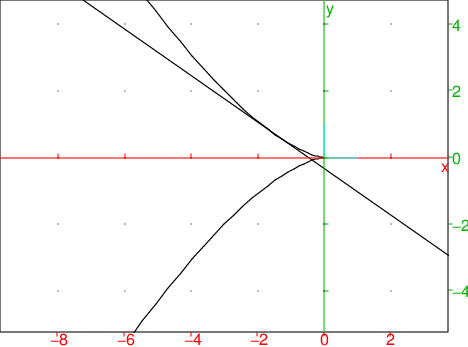
\includegraphics[width=\textwidth]{desolve}\\
en faisant bouger le curseur $m$ on voit que les droites enveloppe la courbe
d'\'equation param\'etrique $x=-3*t^2,y=-2*t^3$
\item 
R\'esoudre :
$$y-xy'=\sqrt{a^2+b^2*y'^2}=0$$
On tape alors :
\begin{center}{\tt desolve(y-x*y'-sqrt(a\verb|^|2+b\verb|^|2*y'\verb|^|2),y)}\end{center}
On obtient :
\begin{center}{\tt [c\_0*x+sqrt(a\verb|^|2+b\verb|^|2*c\_0\verb|^|2), [-b\verb|^|2*2*` t`*(sqrt(a\verb|^|2+b\verb|^|2*` t`\verb|^|2))\verb|^|-1/2,-` t`*b\verb|^|2*2*` t`*(sqrt(a\verb|^|2+b\verb|^|2*` t`\verb|^|2))\verb|^|-1/2+sqrt(a\verb|^|2+b\verb|^|2*` t`\verb|^|2)]]}\end{center}
\end{enumerate}
\item R\'esoudre le syst\`eme diff\'erentiel :
$ u'(t)=u(t)+2v(t)+t$\\
$v'(t)=2u(t)+v(t)+t+1$\\
Puis trouver les solutions de ce syt\`eme qui v\'erifie $u(0=1,v(0)=2$
On tape :
\begin{center}{\tt desolve(y'=[[1,2],[2,1]]*y+[x,x+1])}\end{center} 
On obtient
\begin{center}{\tt [[(9*exp(-x)+5*exp(3*x)+9*c\_0*exp(-x)+9*c\_0*exp(3*x)- 9*c\_1*exp(-x)+9*c\_1*exp(3*x)-6*x-14)/18, (-9*exp(-x)+5*exp(3*x)-9*c\_0*exp(-x)+ 9*c\_0*exp(3*x)+9*c\_1*exp(-x)+9*c\_1*exp(3*x)-6*x+4)/18]]}\end{center}
cela donne les expressions de $u(x)$ et $v(x)$.\\
Ou on tape :
\begin{center}{\tt desolve(y'=[[1,2],[2,1]]*y+[t,t+1],t,y)}\end{center} 
ou on tape :
\begin{center}{\tt desolve(z'=[[1,2],[2,1]]*z+[t,t+1],t,z)}\end{center} 
ou on tape :
\begin{center}{\tt desolve(z'=[[1,2],[2,1]]*z+[t,t+1],z(t))}\end{center}
On obtient
\begin{center}{\tt [[(9*exp(-t)+5*exp(3*t)+9*c\_0*exp(-t)+9*c\_0*exp(3*t)- 9*c\_1*exp(-t)+9*c\_1*exp(3*t)-6*t-14)/18, (-9*exp(-t)+5*exp(3*t)-9*c\_0*exp(-t)+ 9*c\_0*exp(3*t)+9*c\_1*exp(-t)+9*c\_1*exp(3*t)-6*t+4)/18]]}\end{center}
cela donne les expressions de $u(t)$ et $v(t)$.\\
Puis, on tape :
\begin{center}{\tt desolve([y'=[[1,2],[2,1]]*y+[x,x+1],y(0)=[1,2]])}\end{center}
On obtient
\begin{center}{\tt [[(16*exp(3*x)-3*x-7)/9,(16*exp(3*x)-3*x+2)/9]]}\end{center}
cela donne les expressions de $u(x)$ et $v(x)$ tels que $u(0)=1$ et $v(0)=2$.\\
Ou on tape :
\begin{center}{\tt desolve([z'=[[1,2],[2,1]]*z+[t,t+1],z(0)=[1,2]],t,z)}\end{center} 
ou on tape :
\begin{center}{\tt desolve([z'=[[1,2],[2,1]]*z+[t,t+1],z(0)=[1,2]],z(t))}\end{center}
On obtient
\begin{center}{\tt [[(16*exp(3*t)-3*t-7)/9,(16*exp(3*t)-3*t+2)/9]]}\end{center}
cela donne les expressions de $u(t)$ et $v(t)$ tels que $u(0)=1$ et $v(0)=2$.
\end{itemize}

\subsection{Transform\'ee de Laplace et transform\'ee de Laplace inverse : {\tt laplace ilaplace invlaplace}}\index{laplace}\index{ilaplace}\index{invlaplace}\label{sec:lap}
{\tt laplace} et {\tt ilaplace} (ou {\tt invlaplace}) ont 1, 2 ou 3 arguments :\\
l'expression que l'on transforme et \'eventuellement le nom de 2 variables.\\
L'expression est une expression de la variable courante 
(ici $x$) ou l'expression que l'on transforme est une expression de la variable
donn\`ee comme deuxi\`eme argument.\\
{\tt laplace} est la transform\'ee de Laplace de l'expression donn\'ee comme
 argument et {\tt ilaplace} (ou {\tt invlaplace}) est la transform\'ee de
 Laplace inverse de l'expression donn\'ee comme argument. Le r\'esultat de 
{\tt laplace} et {\tt ilaplace} (ou {\tt invlaplace}) est une expression de 
variable le troisi\`eme argument ou par d\'efaut le second argument ou par d\'efaut $x$.\\
{\bf Attention} le second argument est le nom de la variable du premier argument
et est ausi le nom de la variable du r\'esultat lorsqu'il n'y a pas de 
3-i\`eme argument, par exemple :{\tt laplace(sin(x),t)} renvoie {\tt sin(x)/t}.   

On utilise la transform\'ee de Laplace ({\tt laplace}) et la transform\'ee
de Laplace inverse ({\tt ilaplace} ou {\tt invlaplace}) pour r\'esoudre des \'equations 
diff\'erentielles lin\'eaires \`a coefficients constants, par exemple :
$$y \prime \prime +p. y \prime+q. y \ =\ f(x)$$ $$ y(0)=a \ y\prime(0)=b$$
En notant ${\mathcal{L}}$ la transform\'ee de Laplace, on a les relations 
suivantes :
\begin{eqnarray*}
{\mathcal{L}}(y)(x)&=&\int_0^{+\infty}e^{-x.u}y(u)du \\
{\mathcal{L}}^{-1}(g)(x)&=&\frac{1}{2i\pi}\int_C e^{z.x}g(z)dz
\end{eqnarray*}
o\`u $ C$ est une courbe ferm\'ee contenant les p\^oles de {\tt g}.\\
{\tt laplace} :\\
On tape :
\begin{center}{\tt laplace(sin(x))}\end{center}
ici on ne pr\'ecise pas la variable, alors l'expression que l'on transforme 
L'expression (ici $\sin(x)$) est une expression de la variable courante 
(ici $x$) et la transform\'ee sera aussi une fonction de la variable $x$.\\
On obtient:
\begin{center}{\tt 1/(x\verb|^|2+1)}\end{center}
Ou on tape :
\begin{center}{\tt laplace(sin(t),t)}\end{center}
ici on pr\'ecise le nom de la variable de la fonction que l'on transforme (ici 
$t$) et ce nom de variable sera utilis\'e pour la transform\'ee de Laplace.\\
On obtient:
\begin{center}{\tt 1/(t\verb|^|2+1)}\end{center}
Ou on tape :
\begin{center}{\tt laplace(sin(t),t,s)}\end{center}
ici on pr\'ecise le nom de la variable de la fonction que l'on transforme (ici
$t$) et le nom de la variable que l'on d\'esire avoir pour la transform\'ee de 
Laplace (ici $s$).\\
On obtient:
\begin{center}{\tt 1/(s\verb|^|2+1)}\end{center}
{\tt ilaplace} ou {\tt invlaplace} :\\
On tape :
\begin{center}{\tt ilaplace(1/(x\verb|^|2+1))}\end{center}
On obtient:
\begin{center}{\tt sin(x)}\end{center}
On tape :
\begin{center}{\tt ilaplace(1/(t\verb|^|2+1),t)}\end{center}
On obtient:
\begin{center}{\tt sin(t)}\end{center}
On tape :
\begin{center}{\tt ilaplace(1/(t\verb|^|2+1),t,x)}\end{center}
On obtient:
\begin{center}{\tt sin(x)}\end{center}

On utilise les propri\'et\'es suivantes :
\begin{eqnarray*}
{\mathcal{L}}(y')(x) &=&-y(0)+x.{\mathcal{L}}(y)(x) \\
{\mathcal{L}}(y'')(x) &=&-y'(0)+x.{\mathcal{L}}(y')(x) \\
 &=& -y'(0)-x.y(0)+x^2.{\mathcal{L}}(y)(x)
\end{eqnarray*}
On a donc si $y \prime \prime(x) +p. y \prime(x)+q. y(x) \ =\ f(x)$ :
\begin{eqnarray*}
{\mathcal{L}}(f)(x) &=&{\mathcal{L}}(y''+p.y'+q.y)(x) \\
&=& -y'(0)-x.y(0)+x^2.{\mathcal{L}}(y)(x)-p.y(0)+p.x.{\mathcal{L}}(y)(x))+q.{\mathcal{L}}(y)(x) \\
&=& (x^2+p.x+q).{\mathcal{L}}(y)(x)-y'(0)-(x+p).y(0)
\end{eqnarray*}
soit, si $a=y(0)$ et $b=y'(0)$ :\\
$${\mathcal{L}}aplace(f)(x)=(x^2+p.x+q).{\mathcal{L}}aplace(y)(x)-(x+p).a-b$$
La solution est alors :
\[ y(x)=
{\mathcal{L}}^{-1}(({\mathcal{L}}(f)(x)+(x+p).a +b)/(x^2+p.x+q))
\]
Exemple :\\
R\'esoudre :
\[ y\prime \prime -6. y\prime+9. y \ =\ x. e^{3. x},
\quad  y(0)=c\_0, \quad y\prime(0)=c\_1
\]
Ici, $p=-6,\ q=9$.\\
On tape :
\begin{center}{\tt laplace(x*exp(3*x))}\end{center}
On obtient :
\begin{center}{\tt 1/(x\verb|^| 2-6*x+9)}\end{center}
On tape :
\begin{center}{\tt ilaplace((1/(x\verb|^|2-6*x+9)+(x-6)*c\_0+c\_1)/(x\verb|^|2-6*x+9))}\end{center}
On obtient 
\begin{center}{\tt (216*x\verb|^|3-3888*x*c\_0+1296*x*c\_1+1296*c\_0)*exp(3*x)/1296}\end{center}
apr\`es simplification et factorisation (commande {\tt factor}) la solution 
$y$ s'\'ecrit :
\begin{center}{\tt (-18*c\_0*x+6*c\_0+x\verb|^|3+6*x*c\_1)*exp(3*x)/6}\end{center}
On peut bien s\^ur taper directement :
\begin{center}{\tt desolve(y''-6*y'+9*y=x*exp(3*x),y)}\end{center}
On obtient bien :
\begin{center}{\tt exp(3*x)*(-18*c\_0*x+6*c\_0+x\verb|^|3+6*x*c\_1)/6}\end{center}

\section{Transform\'ee en z et transform\'ee en z inverse}
\subsection{Transform\'ee en $z$ d'une suite, la fonction $ztrans$ : {\tt ztrans}}\index{ztrans}
\noindent{\tt ztrans} a un ou trois arguments :
\begin{itemize}
\item une suite donn\'ee par son terme g\'en\'eral $a_x$ : la 
variable utilis\'ee pour d\'efinir le terme g\'en\'eral est $x$ et $x$ sera 
aussi le nom de la variable utilis\'ee dans la fonction renvoy\'ee par 
{\tt ztrans}
\item une suite donn\'ee par son terme g\'en\'eral  $a_n$, le 
nom de la variable utilis\'ee pour d\'efinir ce terme g\'en\'eral (ici $n$) et
le nom de la variable utilis\'ee dans la fonction renvoy\'ee par {\tt ztrans}
(par exemple $z$).
\end{itemize} 
{\tt ztrans} calcule la transform\'ee en $z$ de la suite donn\'ee en argument.\\
On a par d\'efinition :\\
si $f(x)=ztrans(a_x)$ on a  
$$f(x)=\sum_{n=0}^{inf} \frac{a_n}{x^n}$$
si $f(z)=ztrans(a_n,n,z)$ on a  
$$f(z)=\sum_{n=0}^{inf} \frac{a_n}{z^n}$$
On tape :
\begin{center}{\tt ztrans(1)}\end{center}
On obtient :
\begin{center}{\tt x/(x-1)}\end{center}
On a en effet :\\
$=\sum_{n=0}^{inf}\frac{1}{x^n}=\frac{1}{1-\frac{1}{x}}=\frac{x}{x-1}$\\
On tape :
\begin{center}{\tt ztrans(1,n,z)}\end{center}
On obtient :
\begin{center}{\tt z/(z-1)}\end{center}
On a en effet :\\
$1+\frac{1}{z}+\frac{1}{z^2}+\frac{1}{z^3}+\frac{1}{z^4}+..=\sum_{n=0}^{inf}\frac{1}{z^n}=\frac{1}{1-\frac{1}{z}}=\frac{z}{(z-1)}$\\
On tape :
\begin{center}{\tt ztrans(x)}\end{center}
On obtient :
\begin{center}{\tt x/(x\verb|^|2-2*x+1)}\end{center}
On tape :
\begin{center}{\tt ztrans(n,n,z)}\end{center}
On obtient :
\begin{center}{\tt z/(z\verb|^|2-2*z+1)}\end{center}
On a en effet :
$\frac{1}{z-1}=\sum_{n=1}^{inf}\frac{1}{z^n}$\\
$\frac{1}{(z-1)^2}=-(\frac{1}{(z-1)})'=\sum_{n=1}^{inf}\frac{n}{z^{n-1}} $\\
Donc $\frac{z}{(z-1)^2}=\sum_{n=1}^{inf}\frac{n}{z^{n}}$

\subsection{Transform\'ee en z inverse d'une fraction rationnelle, la fonction $invztrans$ : {\tt invztrans}}\index{ invztrans}
\noindent{\tt invztrans} a un ou trois arguments :
\begin{itemize}
\item  une fraction rationnelle donn\'ee par son expression en utilisant la 
variable $x$ et $x$ sera aussi le nom de la variable utilis\'ee dans la 
fonction renvoy\'ee par, {\tt ztrans},
\item trois arguments une fraction rationnelle donn\'ee par son expression, le 
nom de la variable utilis\'ee pour d\'efinir cette expression (paz exemple la 
variable $z$), et le nom de la variable utilis\'ee dans la fonction renvoy\'ee 
par {\tt invztrans} (par exemple $n$).
\end{itemize} 
{\tt invztrans} calcule la transform\'ee en $z$ inverse de la fraction 
rationnelle donn\'ee en argument.\\
On a par d\'efinition :\\
si $invztrans(R_x)=a_x$ on a  
$$R_x=\sum_{n=0}^{inf} \frac{a_n}{x^n}$$
si $a_n=invztrans(R_z,z,n)$ on a  
$$R_z=\sum_{n=0}^{inf} \frac{a_n}{z^n}$$
On tape :
\begin{center}{\tt  invztrans(x/(x-1))}\end{center}
On obtient :
\begin{center}{\tt 1}\end{center}
On tape :
\begin{center}{\tt  invztrans(z/(z-1),z,n)}\end{center}
On obtient :
\begin{center}{\tt 1}\end{center}
On a en effet :
$\frac{z}{(z-1)}=\frac{1}{1-\frac{1}{z}}=1+\frac{1}{z}+\frac{1}{z^2}+\frac{1}{z^3}+\frac{1}{z^4}+..=\sum_{n=0}^{inf}\frac{1}{z^n} $
On tape :
\begin{center}{\tt  invztrans(x/(x-1)\verb|^|2)}\end{center}
On obtient :
\begin{center}{\tt x}\end{center}
On tape :
\begin{center}{\tt  invztrans(z/(z-1)\verb|^|2,z,n)}\end{center}
On obtient :
\begin{center}{\tt n}\end{center}

\section{Autres fonctions}
\subsection{N\'egliger les petites valeurs : {\tt epsilon2zero}}
\index{epsilon2zero} \label{sec:epsilon2zero}
\noindent{\tt epsilon2zero} a comme param\`etre une expression de {\tt x}.\\ 
{\tt epsilon2zero} renvoie l'expression o\`u les valeurs plus petites que 
{\tt epsilon} ont \'et\'e remplac\'ees par z\'ero dans l'expression non 
\'evalu\'ee.\\
La valeur de {\tt epsilon}\index{epsilon} peut \^etre chang\'e dans la 
configuration du {\tt cas} (par d\'efaut {\tt epsilon=1e-10}).\\
On tape :
\begin{center}{\tt epsilon2zero(1e-13+x) }\end{center}
On obtient (avec {\tt epsilon=1e-10}) :
\begin{center}{\tt 0+x}\end{center}
On tape :
\begin{center}{\tt epsilon2zero((1e-13+x)*100000) }\end{center}
On obtient (avec {\tt epsilon=1e-10}) :
\begin{center}{\tt (0+x)*100000}\end{center}
On tape :
\begin{center}{\tt epsilon2zero(0.001+x) }\end{center}
On obtient (avec {\tt epsilon=0.0001}) :
\begin{center}{\tt 0.001+x}\end{center}

\subsection{Liste des variables : {\tt lname indets}}\index{lname}\index{indets}
\noindent{\tt lname} (ou {\tt indets}) a comme param\`etre une expression.\\ 
{\tt lname} (ou {\tt indets}) renvoie un vecteur de composantes le nom des 
variables symboliques utilis\'ees dans cette expression.\\
On tape :
\begin{center}{\tt lname(x*y*sin(x))}\end{center}
On obtient :
\begin{center}{\tt  [x,y]}\end{center}
On tape :
\begin{center}{\tt a:=2;assume(b>0);assume(c=3);}\end{center}
\begin{center}{\tt lname(a*x\verb|^|2+b*x+c)}\end{center}
On obtient :
\begin{center}{\tt  [x,b,c]}\end{center}

\subsection{Liste des variables et des expressions : {\tt lvar}}\index{lvar}\label{sec:lvar}
\noindent{\tt lvar} a  comme param\`etre une expression.\\
{\tt lvar} renvoie un vecteur de composantes les noms de variables et des 
expressions dont cette expression d\'epend rationnellement.\\
On tape :
\begin{center}{\tt lvar(x*y*sin(x)\verb|^|2+ln(x)*cos(y))}\end{center}
On obtient :
\begin{center}{\tt [x,y,sin(x)]}\end{center}
On tape :
\begin{center}{\tt lvar(x*y*sin(x)\verb|^|2)}\end{center}
On obtient :
\begin{center}{\tt [x,y,sin(x),ln(x),cos(y)]}\end{center}
On tape :
\begin{center}{\tt lvar(y+x*sqrt(z)+y*sin(x))}\end{center}
On obtient :
\begin{center}{\tt [y,x,sqrt(z),sin(x)]}\end{center}

\subsection{Liste des variables et des expressions alg\'ebriques : {\tt algvar}}\index{algvar}
\noindent{\tt algvar} a comme param\`etre une expression.\\ 
{\tt algvar} renvoie un vecteur de composantes le nom des variables 
symboliques, par ordre d'extension algebriques, utilis\'ees dans cette 
expression.\\
On tape :
\begin{center}{\tt algvar(y+x*sqrt(z))}\end{center}
On obtient :
\begin{center}{\tt  [[y,x],[z]]}\end{center}
On tape :
\begin{center}{\tt algvar(y*sqrt(x)*sqrt(z))}\end{center}
On obtient :
\begin{center}{\tt  [[y],[z],[x]]}\end{center}
On tape :
\begin{center}{\tt algvar(y*sqrt(x*z))}\end{center}
On obtient :
\begin{center}{\tt  [[y],[x,z]]}\end{center}
On tape :
\begin{center}{\tt algvar(y+x*sqrt(z)+y*sin(x))}\end{center}
On obtient :
\begin{center}{\tt [[x,y,sin(x)],[z]]}\end{center}

\subsection{Test de la pr\'esence d'une variable dans une expression : {\tt has}}\index{has|textbf}
\noindent{\tt has} a  comme param\`etre une expression et le nom d'une 
variable.\\
{\tt has} renvoie {\tt 1}, ou {\tt 0}, selon que la variable est pr\'esente, 
ou non pr\'esente, dans l'expression.\\
On tape :
\begin{center}{\tt has(x*y*sin(x),y)}\end{center}
On obtient :
\begin{center}{\tt  1}\end{center}
On tape :
\begin{center}{\tt has(x*y*sin(x),z)}\end{center}
On obtient :
\begin{center}{\tt  0}\end{center}
\subsection{Pseudo-variable g\'erant les extensions alg\'ebriques : {\tt keep\_algext}}\index{keep\_algext}
{\tt keep\_algext} est une pseudo-variable qui laisse les extensions 
alg\'ebriques telles quelles ({\tt keep\_algext:=1}) ou tente de les
 r\'e\'ecrire ({\tt keep\_algext:=0}).
\subsection{\'Evaluation num\'erique : {\tt evalf}}\index{evalf}
\noindent{\tt evalf} a comme param\`etre une expression ou une matrice.\\
{\tt evalf} renvoie la valeur num\'erique de
l'expression ou de la matrice.\\
On tape :
\begin{center}{\tt evalf(sqrt(2))}\end{center} 
On obtient :
\begin{center}{\tt 1.41421356237}\end{center}
On tape :
\begin{center}{\tt evalf([[1,sqrt(2)],[0,1]])}\end{center} 
On obtient :
\begin{center}{\tt [[1.0,1.41421356237],[0.0,1.0]]}\end{center}

\subsection{Approximation rationnelle : {\tt float2rational exact}}\index{float2rational}\index{exact}
\noindent{\tt float2rational} (ou {\tt exact}) a comme param\`etre une 
expression num\'erique r\'eelle.\\
{\tt float2rational} donne une approximation rationnelle de tous les nombres 
d\'ecimaux $r$ contenus dans l'expression \`a 
moins de {\tt epsilon} c'est\`a dire 
$|r-\mbox{\tt float2rational}(r)|<\epsilon$ o\`u $\epsilon$ est d\'efinit par
{\tt epsilon} dans la configuration du {\tt cas} (menu {\tt Cfg} , ou 
commande {\tt cas\_setup}).\\
On tape :
\begin{center}{\tt float2rational(1.5)}\end{center}
On obtient :
\begin{center}{\tt 3/2}\end{center}
On tape :
\begin{center}{\tt float2rational(1.414)}\end{center}
On obtient :
\begin{center}{\tt 707/500}\end{center}
On tape :
\begin{center}{\tt float2rational(0.156381102937*2)}\end{center}
On obtient :
\begin{center}{\tt 5144/16447}\end{center}
On tape :
\begin{center}{\tt float2rational(1.41421356237)}\end{center}
On obtient :
\begin{center}{\tt 114243/80782}\end{center}
On tape :
\begin{center}{\tt float2rational(1.41421356237\verb|^|2)}\end{center}
On obtient :
\begin{center}{\tt 2}\end{center}
\section{Lejour de la semaine : {\tt dayofweek}}\index{dayofweek|textbf}
\noindent{\tt dayofweek(j,m,a} renvoie 0 pour dimanche, 1 pour lundi ...6 pour 
samedi pour çindiquer le jour de la semaine qui correspond \`a la date 
donn\'ee en argument date sup\'erieure au 15 octobre 1582.
On tape :
\begin{center}{\tt dayofweek(15,10,1582)}\end{center}
On obtient :
\begin{center}{\tt 5}\end{center}
Donc le 15 octobre 1582 \'etait un vendredi. En effet le calendrier gr\'egorien 
date du 15 octobre 1582 (le lendemain du jeudi 4 octobre 1582 fut le vendredi 
15 octobre 1582 car avant les ann\`ees bissextiles \'etaient tous les 4 ans ce 
qui donne  comme dur\'ee moyenne de l'ann\`ee civile 365.25 jours alors que la 
r\'evolution de la terre autour du soleil est plus courte (365.242 jours) 
d'o\`u un d\'ecalage qui \'etait de 10 jours en 1582. \\
Avec la nouvelle r\`egle (la derni\`ere ann\'ee de chaque si\'ecle est 
bissextile si son mill\'esime est divisble par 400) l'\'ecart n'est plus 
que de l'ordre de 1 jour tous les 3000 ans.\\
On tape :
\begin{center}{\tt dayofweek(1,10,2014)}\end{center}
On obtient :
\begin{center}{\tt 3}\end{center}
Donc le 1ier octobre 2014 \'etait un mercredi.

\chapter{Propri\'et\'es m\'etriques des courbes planes ou gauches}
\section{Tangente et plans tangents}
Soit une courbe $\Gamma$ lieu des points $M=M(t)$ de coordonn\'ees 
$x(t),y(t),z(t)$ dans un rep\`ere orthonorm\'e $Oxyz$.\\
Le vecteur directeur de la tangente \`a $\Gamma$ est le premier vecteur 
$T=\displaystyle \frac{d^pM}{dt^p}$ qui ne soit pas nul.\\
\`A chaque tangente  en $M$ on associe :\\
une infinit\'e de plans tangents qui sont les plans contenant $T$ et\\
une infinit\'e de normales qui sont toutes perpendiculaires  en $M$ \`a $T$ et 
qui forment le plan normal en $M$.\\
\section{Place de la courbe par rapport \`a un plan tangent}
Comment se place la courbe par rapport \`a un certain plan $\Pi$ tangent en $M$
\`a $\Gamma$ ?
Soit $N$ la normale qui est perpendiculaire \`a $\Pi$ en $M$.\\
Soit $M_1$ un point de $\Gamma$ et $m_1$ la projection de $M_1$ sur $T$.\\
$Mm_1$ a le sens de $\displaystyle(t_1-t)^p\frac{d^pM}{dt^p}$ ($\displaystyle \frac{d^pM}{dt^p}$ \'etant le premier vecteur deriv\'e de $OM$ non nul.\\
$M_1$ est dans la m\^eme r\'egion par rapport \`a $Pi$ que le vecteur
$\displaystyle(t_1-t)^q\frac{d^qM}{dt^q}$ o\`u $\displaystyle(t_1-t)^q\frac{d^qM}{dt^q}$ est la premi\`ere des d\'eriv\'ees suivantes qui soit non nulles et non situ\'es dans $Pi$ 

\section{Notion d'abscisse curviligne : {\tt }}\index{}
Soit une courbe $\Gamma$ lieu des points $M=M(t)$ de coordonn\'ees 
$x(t),y(t),z(t)$ dans un rep\`ere orthonorm\'e $Oxyz$.\\
On suppose que $x(t),y(t),z(t)$  sonr continues , d\'erivables et \`a 
d\'eriv\'ees continues.\\
On note $\displaystyle \frac{dM}{dt}$ le vecteur de coordonn\'ees 
$x'(t),y'(t),z'(t)$ qui est un vecteur tangent \`a $\Gamma$ quelque soit $t$.\\
On introduit un nouveau param\'etre $s$ pour $\Gamma$ pour que 
$\displaystyle \frac{dM}{ds}$ soit unitaire c'est \`a dire tel que :\\
$ds^2=dx^2+dy^2+dz^2$\\
Cette relation d\'efinie da d\'eriv\'ee de $s$ par rapport \`a $t$ au signe 
pr\`es :\\
$\displaystyle \frac{ds}{dt}=\sqrt{x'(t)^2+y'(t)^2+z'(t)^2}$ si on oriente 
$\Gamma$ selon les $t$ croissants,\\
$\displaystyle \frac{ds}{dt}=-\sqrt{x'(t)^2+y'(t)^2+z'(t)^2}$ si on oriente 
$\Gamma$ selon les $t$ d\'ecroissants.\\
On appelle {\bf abscisse curviligne} \`a partir de l'origine $M_0=M(t_0)$, la 
fonction $s(t)$ ayant pour d\'eriv\'ee :
$\displaystyle \frac{ds}{dt}=\sqrt{x'(t)^2+y'(t)^2+z'(t)^2}$ (ou $\displaystyle \frac{ds}{dt}=-\sqrt{x'(t)^2+y'(t)^2+z'(t)^2}$ selon l'orientation choisie)
et telle que $s(t_0)=0$.\\
La tangente orient\'ee de $\Gamma$ au point $M$ est alors :\\
$\tau=\displaystyle \frac{dM}{ds}$ qui est le vecteur :\\
en coordonn\'ees cart\'esiennes :
$\displaystyle \tau=(\frac{dx}{ds},\frac{dy}{ds},\frac{dz}{ds})$.\\
en coordonn\'ees semi-polaires
$\displaystyle \tau=(\frac{d\rho}{ds},\frac{\rho d\theta}{ds},\frac{dz}{ds})$.
\section{Le plan osculateur}
Soit une courbe $\Gamma$ lieu des points $M=M(t)$ de coordonn\'ees 
$x(t),y(t),z(t)$ dans un rep\`ere orthonorm\'e $Oxyz$.\\
Le vecteur directeur de la tangente \`a $\Gamma$ est le premier vecteur 
$\displaystyle \frac{d^pM}{dt^p}$ qui ne soit pas nul.\\
Consid\'erons le cas le plus courant o\`u 
$\displaystyle \frac{dM}{dt}$ et $\displaystyle \frac{d^2M}{dt^2}$ sont non 
nuls et non colin\'eaires.
Le {\bf plan osculateur} est le plan  des deux vecteurs 
$\displaystyle \frac{dM}{dt}$ et $\displaystyle \frac{d^2M}{dt^2}$ et plus 
g\'en\'eralement le plan  des deux premiers vecteurs :
$\displaystyle \frac{d^pM}{dt^p}$ et $\displaystyle \frac{d^{p+h}M}{dt^{p+h}}$ qui
 ne sont ni nuls et ni colin\'eaires.\\
{\bf Remarque} Le plan osculateur comme la tangente ne d\'epend pas du 
param\`etre utilis\'e.\\
Le vecteur $\displaystyle \frac{d^2M}{ds^2}=\frac{d\tau}{ds}$ est donc dans le
 plan osculateur et il est orthogonal \`a $\tau$.
On appelle {\bf normale principale} l'intersection du plan normal (plan 
perpendiculaire \`a la tangente $\tau$) et du plan osculateur.\\
Soit $n$ le vecteur unitaire de la normale principale orient\'ee dans le sens 
de la concavit\'e i.e. selon $\frac{d\tau}{ds}$
\section{Courbure et Cercle osculateur: {\tt curvature, courbure}}\index{curvature}\index{courbure}
\subsection{Premi\`ere formule de Frenet}
On \'etudie le vecteur $\displaystyle \frac{d^2M}{ds^2}=\frac{d\tau}{ds}$.\\
$\displaystyle \frac{d^2M}{ds^2}$ est situ\'e dans le plan osculateur et est 
situ\'e par rapport \`a un plan non osculateur selon la concavit\'e de $\Gamma$.
$\displaystyle \frac{d^2M}{ds^2}$ est perpendiculaire \`a $\tau$ puisque
$\tau$ est unitaire.\\
Soit $n$ le vecteur unitaire de la normale principale orient\'ee dans le sens 
de la concavit\'e i.e. selon $\frac{d\tau}{ds}$, il exite  un scalaire positif 
$R$ tel que :
$$\displaystyle \frac{d\tau}{ds}=\frac{n}{R}$$
On dit que $R$ est le {\bf rayon de courbure} de $\Gamma$ en $M$ et on appelle 
{\bf centre de courbure} de $\Gamma$ en $M$, le point $C$ d\'efini par :\\
$MC=Rn$\\
La courbure de $\Gamma$ au point $M$ est \'egale \`a $\frac{1}{R}$.
\subsection{Courbure : {\tt curvature, courbure}}\index{curvature}\index{courbure}
\subsection{Cercle osculateur : {\tt osculating\_circle}}
\index{cercle\_osculateur}\index{osculating\_circle}
On appelle cercle osculateur en $M$ \`a $\Gamma$, la limite du cercle passant 
par $M$ et tangent en $M_0$ \`a $\Gamma$, quand $M$ tend vers $M_0$ en 
d\'ecrivant $\Gamma$.\\
Le centre du cercle osculateur en $M$ \`a $\Gamma$ est le centre de courbure au
point $M$ de $\Gamma$.\\
\subsection{Applications}
Trouver la courbure et le centre de courbure de la spirale logarithmique :\\
$\rho=3e^{\theta/2}$ en un point $M$ de coordonn\'ees :\\
$\rho\cos(\theta),\rho\sin(\theta)$ et \\
en un point $M_0$ de coordonn\'ees :\\
$3e^{7/2}\cos(7),3e^{7/2}\sin(7)$.\\
On tape :\\
{\tt trigcos(courbure([3*exp(t/2)*cos(t),3*exp(t/2)*sin(t)],t))}\\
On obtient le rayon de courbure au point $M$ d'affixe 
$3*\exp(1/2)*(\cos(1)+i*\sin(1))$:\\
{\tt 2*sqrt(5)/(15*exp(t/2))}\\
On tape pour avoir le rayon de courbure au point $M_0$ d'affixe 
$3*\exp(7/2)*(\cos(7)+i*\sin(7))$:\\
{\tt trigcos(courbure([3*exp(t/2)*cos(t),3*exp(t/2)*sin(t)],t,7))}\\
On obtient :\\
{\tt 2*sqrt(5)/(15*exp(7/2))}\\
Pour avoir l'\'equation du cercle osculateur en $M$, on tape :\\
{\tt trigcos(equation(cercle\_osculateur([3*exp(t/2)*cos(t),3*exp(t/2)*sin(t)],t)))}\\
On obtient :\\
{\tt x\verb|^|2+y\verb|^|2+9*exp(t/2)\verb|^|2/4+3*x*exp(t/2)*sin(t)-3*y*exp(t/2)*cos(t)=(45*exp(t/2)\verb|^|2/4)}\\
Pour avoir l'\'equation du cercle osculateur en $M_0$, on tape :\\
{\tt trigcos(equation(cercle\_osculateur([3*exp(t/2)*cos(t),3*exp(t/2)*sin(t)],t,7)))}\\
On obtient :\\
{\tt x\verb|^|2+y\verb|^|2+9*exp(7/2)\verb|^|2/4+3*x*exp(7/2)*sin(7)-3*y*exp(7/2)*cos(7)=(45*exp(7/2)\verb|^|2/4)}\\
Pour avoir l'affixe du centre du cercle osculateur en $M$, on tape :\\
{\tt affixe(centre(cercle\_osculateur([3*exp(t/2)*cos(t),3*exp(t/2)*sin(t)],t)))}\\
On obtient :\\
{\tt (3*i)*exp(t/2)*cos(t)/2-3*exp(t/2)*sin(t)/2)}\\
Pour avoir l'affixe du centre  du cercle osculateur en $M_0$, on tape :\\
{\tt affixe(centre(cercle\_osculateur([3*exp(t/2)*cos(t),3*exp(t/2)*sin(t)],t,7)))}\\
On obtient :\\
{\tt (3*i)*exp(7/2)*cos(7)/2-3*exp(7/2)*sin(7)/2}\\
On tape :\\
{\tt plotparam(3*exp(t/2)*(cos(t)+i*sin(t)));}\\
{\tt M0:=point(3*exp(7/2)*(cos(7)+i*sin(7)));}\\
{\tt C:=centre(cercle\_osculateur([3*exp(t/2)*cos(t),3*exp(t/2)*sin(t)],t,7));}\\
{\tt cercle\_osculateur([3*exp(t/2)*cos(t),3*exp(t/2)*sin(t)],t,7,affichage=1)}\\
{\tt segment(C,M0)}\\
{\tt tangente(plotparam(3*exp(t/2)*exp(i*t),t),7);}\\
{\tt demi\_droite(0,M0);}\\
{\tt demi\_droite(0,C);}\\
On obtient :\\
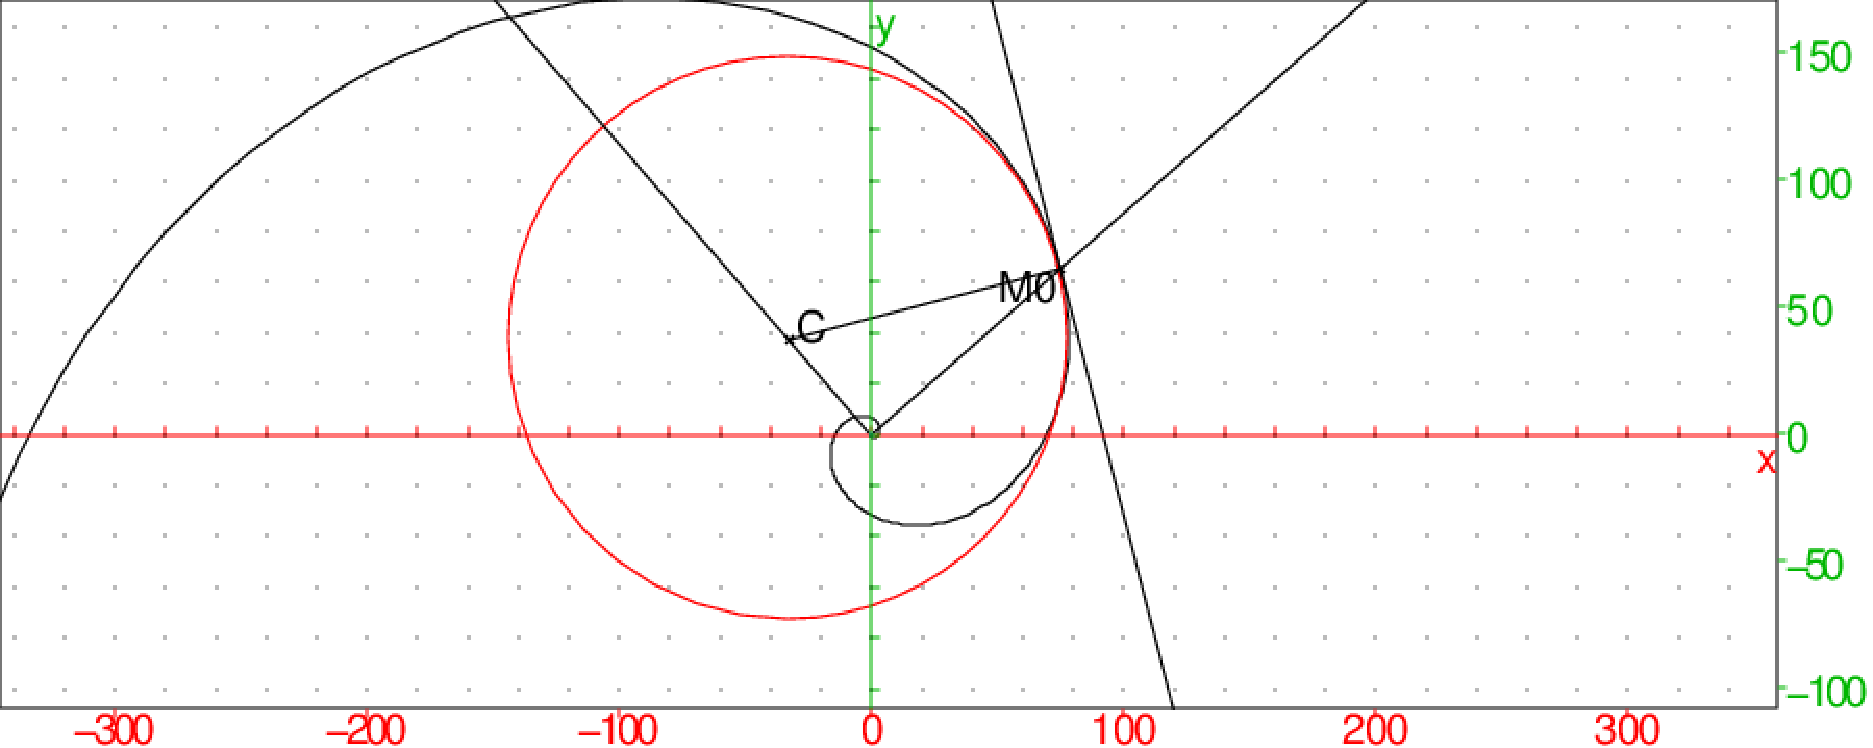
\includegraphics[width=\textwidth]{courbure}
\section{Torsion }
\subsection{Tri\`edre de Frenet}
Aux vecteurs $\tau=\displaystyle \frac{dM}{ds}$ et $n$ on ajoute le vecteur
initaire $b=\tau \wedge n$ : le tri\`edre de Frenet en un point $M$ de 
$\Gamma$ est le tri\`edre $\tau, n, b$ ($\tau$ est la tangente $n$ est la 
normale principale et $b$ est la binormale (c'est la perpendiculaire au plan 
osculateur).
\subsection{Deuxi\`eme et troisi\`eme formule de Frenet}
En d\'erivant $b=\tau \wedge n$ on obtient :\\
$\displaystyle \frac{db}{ds}=\tau \wedge \frac{dn}{ds}$\\
$\displaystyle \frac{db}{ds}$ estdonc parall\`ele \`a $n$ car orthogonal \`a 
$\tau$ et \`a $b$.
Donc il existe un scalaire $T$ appel\'e rayon de torsion de $\Gamma$ au point 
$M$ tel que :
$$ \frac{db}{ds}= \frac{n}{T}$$
c'est la premi\`ere formule de Frenet.\\
On a aussi :\\
$n=b\wedge \tau$  donc en d\'erivant on a :\\
$\displaystyle \frac{dn}{ds}=\frac{db}{ds} \wedge\tau +b\wedge \frac{d\tau}{ds}$\\
$\displaystyle \frac{dn}{ds}=\frac{n}{T} \wedge\tau +b\wedge \frac{n}{R}$\\
ou encore :
$$\frac{dn}{ds}=-\frac{\tau}{R}-\frac{b}{T}$$
c'est la deuxi\`erme formule de Frenet.\\
La torsion de  de $\Gamma$ au point $M$ est \'egale \`a $\frac{1}{T}$.
\section{Cas des courbes planes}
Lorsque $\Gamma$ est une courbe du plan $Oxy$ : son plan osculateur est le plan $Oxy$.\\
La torsion d'une courbe plane est nulle.\\
Soit $\alpha$ l'angle $(Ox,\tau$. On a alors :\\
$\displaystyle \frac{1}{R}\frac{d\alpha}{ds}$ et donc :\\
$\displaystyle \frac{ds}{d\alpha}=R$\\
Soit $\nu$ tel que $(\tau \nu)=\pi/2$, on a ;\\
$d\tau =\nu d\alpha$ et si $c$ est le centre de courbure en $M$ on  a :\\
$MC=\displaystyle \frac{ds}{d\alpha}\nu$
\section{D\'evelopp\'ee d'une courbe plane : {\tt evolute}}\index{evolute}\index{developpee}
On appelle d\'evelopp\'ee d'une courbe plane $\Gamma$, le lieu des centres de 
courbure de  $\Gamma$ : c'est aussi l'enveloppe de ses normales.
{\bf Exemple}\\
Trouver la d\'evelopp\'ee de la spirale logarithmique :\\
$\rho=3e^{\theta/2}$.\\
On tape :\\
{\tt developpee([3*exp(t/2)*cos(t),3*exp(t/2)*sin(t)],t,affichage=2))}\\
On obtient :\\
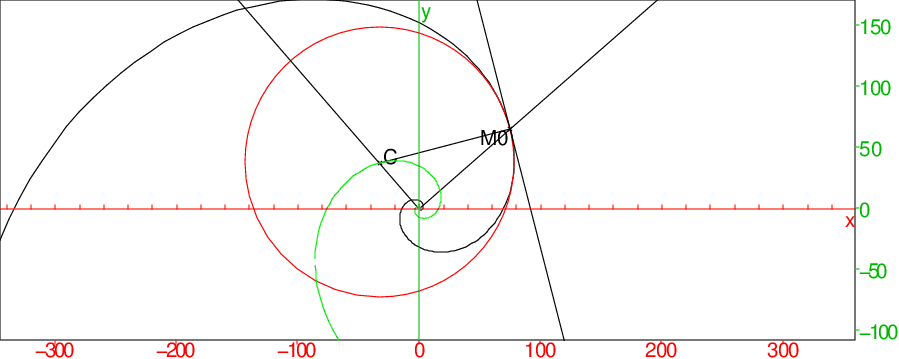
\includegraphics[width=\textwidth]{courbure1}
\section{D\'eveloppante d'une courbe plane}
On appelle d\'eveloppante d'une courbe plane  $\Gamma$ les courbes admettant 
 $\Gamma$ comme d\'evelopp\'ee.



\chapter{Les fonctions de statistique}\label{sec:stat}
\section{Les fonctions de {\tt Xcas} de statistique \`a 1 variable}
On va d\'ecrire les diff\'erentes fonctions statistiques sur un exemple :\\
avec  la liste {\tt A:=[0,1,2,3,4,5,6,7,8,9,10,11]} \\
- en prenant comme s\'erie statistique d'effectif 1 la liste {\tt A}, ou \\
- en prenant comme s\'erie statistique la liste {\tt A} avec comme  effectifs 
encore la liste {\tt A}.\\
On tape :\\
{\tt A:=[0,1,2,3,4,5,6,7,8,9,10,11]}\\
On pourra se reporter aussi \`a \ref{sec:statlist} lorsque les arguments sont 
des listes et \`a \ref{sec:statmat}  lorsque les arguments sont des matrices.
\subsection{La moyenne : {\tt mean moyenne}}\index{mean|textbf} \index{moyenne|textbf}
\noindent{\tt mean} calcule la moyenne num\'erique des \'el\'ements d'une 
liste (ou de chaque colonne d'une matrice).\\
On tape :
\begin{center}{\tt A:=[0,1,2,3,4,5,6,7,8,9,10,11]}\end{center}
\begin{center}{\tt mean(A)}\end{center}
On obtient :
\begin{center}{\tt 11/2}\end{center}
En effet (0+1+...+11)=66 et 66/12=11/2\\
On tape :
\begin{center}{\tt mean([[1,2],[3,4]])}\end{center}
On obtient :
\begin{center}{\tt [2,3]}\end{center}
En effet (1+3)/2=2 et (2+4)/2=3.\\
{\tt mean} calcule la moyenne num\'erique des \'el\'ements d'une 
liste (respectivement de chaque  colonne d'une matrice) pond\'er\'ee par une liste (respectivement
 matrice) de m\^eme taille donn\'ee comme deuxi\`eme argument.\\
On tape :
\begin{center}{\tt A:=[0,1,2,3,4,5,6,7,8,9,10,11]}\end{center}
\begin{center}{\tt mean(A,A)}\end{center}
On obtient :
\begin{center}{\tt 23/3}\end{center}
En effet : 1*1+2*2+..11*11=23*12*11/6=23*2*11 et 1+2+..11=66 donc:\\
{\tt mean(A,A)}=23*2*11/66=23/3\\
On tape :
\begin{center}{\tt mean([[1,2],[3,4]],[[1,2],[3,4]])}\end{center}
On obtient :
\begin{center}{\tt [5/2,10/3]}\end{center}
En effet : (1*1+3*3)/(1+3)=5/2 et (2*2+4*4)/(2+4)=10/3
\subsection{L'\'ecart-type : {\tt stddev ecart\_type}}\index{stddev|textbf}\index{ecart\_type|textbf}
\noindent{\tt stddev} calcule l'\'ecart-type num\'erique des \'el\'ements 
d'une liste (ou de chaque colonne d'une matrice).\\
On tape :
\begin{center}{\tt A:=[0,1,2,3,4,5,6,7,8,9,10,11]}\end{center}
\begin{center}{\tt stddev(A)}\end{center}
On obtient :
\begin{center}{\tt  sqrt(143/12)}\end{center}
On tape :
\begin{center}{\tt stddev([[1,2],[3,4]])}\end{center}
On obtient :
\begin{center}{\tt [1,1]}\end{center}
{\tt stddev} calcule l'\'ecart-type num\'erique des \'el\'ements d'une 
liste pond\'er\'ee par une autre liste donn\'ee comme deuxi\`eme argument.\\
On tape :
\begin{center}{\tt A:=[0,1,2,3,4,5,6,7,8,9,10,11]}\end{center}
\begin{center}{\tt stddev(A,A)}\end{center}
On obtient :
\begin{center}{\tt  sqrt(65/9)}\end{center}
\subsection{L'\'ecart-type de la population : {\tt ecart\_type\_population stddevp stdDev}}\index{stddevp|textbf}\index{stdDev|textbf}\index{ecart\_type\_population|textbf}
\noindent{\tt stddevp} (ou {\tt stdDev}) a comme argument une (ou deux) liste(s) :\\
{\tt stddevp(l)} calcule une estimation l'\'ecart-type num\'erique de la 
population dont est issu l'\'echantillon d\'ecrit par les  \'el\'ements de la  
liste {\tt l}, de longueur {\tt n}, donn\'ee en argument ({\tt size(l)=n} et 
{\tt n} doit \^etre grand). On a :\\
{\tt stddevp(l)\verb|^|2=n/(n-1)* stddev(l)\verb|^|2}.\\
On tape :
\begin{center}{\tt A:=[0,1,2,3,4,5,6,7,8,9,10,11]}\end{center}
\begin{center}{\tt stddevp(A)}\end{center}
On obtient :
\begin{center}{\tt  sqrt(13)}\end{center}
En effet :
{\tt n=size(A)=12} et {\tt 12/11*stddev(A)\verb|^|2=12/11*143/12=13}.\\
On tape :
\begin{center}{\tt stddevp([[1,2],[3,4]])}\end{center}
On obtient :
\begin{center}{\tt [sqrt(2),sqrt(2)]}\end{center}
\ \\
{\tt stddevp(l1,l2)} calcule l'\'ecart-type num\'erique de la population dont 
est issu l'\'echantillon d\'ecrit par les \'el\'ements d'une 
liste {\tt l1} pond\'er\'ee par une autre liste {\tt l2} donn\'ee comme
 deuxi\`eme argument.\\
On a :\\
{\tt stddevp(l1,l2)\verb|^|2=n/(n-1)* stddev(l1,l2)\verb|^|2} si {\tt n} est la
taille de l'\'echantillon c'est \`a dire si {\tt n} est la somme de la liste 
{\tt l2} ({\tt sum(l2)=n}).\\
On tape :
\begin{center}{\tt stddevp(A,A)}\end{center}
On obtient :
\begin{center}{\tt  sqrt(22/3)}\end{center}
En effet {\tt sum(A)=66} et
 $\displaystyle \frac{22}{3}=\frac{66}{65}*\frac{65}{9}$
{\bf Remarque}
{\tt stddev} est l'\'ecart type apr\`es division par {\tt n} (taille de 
l'\'echantillon) alors que {\tt stddevp} et son synonyme {\tt stdDev} (nom de 
commande TI) est divis\'e par 
{\tt n-1} et donne l'estimateur non biais\'e de l'\'ecart-type d'une population
\`a partir de l'\'ecart-type calcul\'e avec un \'echantillon (la division
par {\tt n-1} permet de supprimer le biais).\\
Pour la variance nous ne donnons qu'une commande (division par {\tt n}),
mais il est tr\`es facile de d\'efinir une "variance d'\'echantillon"
en prenant le carr\'e de l'\'ecart-type {\tt stddevp}.

\subsection{La variance : {\tt variance}}\index{variance|textbf}
\noindent{\tt variance} calcule la variance  num\'erique des \'el\'ements 
d'une liste.\\
On tape :
\begin{center}{\tt A:=[0,1,2,3,4,5,6,7,8,9,10,11]}\end{center}
\begin{center}{\tt variance(A)}\end{center}
On obtient :
\begin{center}{\tt 143/12}\end{center}
\ \\
{\tt variance} calcule la variance  num\'erique des \'el\'ements d'une 
liste pond\'er\'ee par une autre liste donn\'ee comme deuxi\`eme argument.\\
On tape :
\begin{center}{\tt A:=[0,1,2,3,4,5,6,7,8,9,10,11]}\end{center}
\begin{center}{\tt variance(A,A)}\end{center}
On obtient :
\begin{center}{\tt  65/9}\end{center}
On tape :
\begin{center}{\tt variance([[1,2],[3,4]])}\end{center}
On obtient :
\begin{center}{\tt [1,1]}\end{center}
\subsection{La m\'ediane : {\tt median}}\index{median|textbf}
\noindent{\tt median} calcule la m\'ediane des \'el\'ements 
d'une liste.\\
On tape :
\begin{center}{\tt A:=[0,1,2,3,4,5,6,7,8,9,10,11]}\end{center}
\begin{center}{\tt median(A)}\end{center}
On obtient :
\begin{center}{\tt 5.0}\end{center}
{\tt median} calcule la m\'ediane num\'erique des \'el\'ements d'une 
liste pond\'er\'ee par une autre liste donn\'ee comme deuxi\`eme argument.\\
On tape :
\begin{center}{\tt A:=[0,1,2,3,4,5,6,7,8,9,10,11]}\end{center}
\begin{center}{\tt  median(A,A)}\end{center}
On obtient :
\begin{center}{\tt 8}\end{center}
On a en effet : $1+2+3+...7=28$ et $9+10+11=30$ il y a donc 28 \'el\'ements 
avant 8 et 30 \'el\'ements apr\`es 8.

\subsection{Diff\'erentes valeurs statistiques : {\tt quartiles}}\index{quartiles|textbf}
\noindent{\tt quartiles} renvoie la matrice colonne form\'ee par : le minimum, 
le premier quartile, la m\'ediane, le troisi\`eme quartile et le maximum des 
\'el\'ements d'une liste.\\
On tape :
\begin{center}{\tt A:=[0,1,2,3,4,5,6,7,8,9,10,11]}\end{center}
\begin{center}{\tt quartiles(A)}\end{center}
On obtient :
\begin{center}{\tt [[0.0],[2.0],[5.0],[8.0],[11.0]]}\end{center}
On tape :
\begin{center}{\tt A:=[0,1,2,3,4,5,6,7,8,9,10,11]}\end{center}
\begin{center}{\tt quartiles(A,A)}\end{center}
On obtient :
\begin{center}{\tt [1,6,8,10,11]}\end{center}

\subsection{Le premier quartile : {\tt quartile1}}\index{quartile1}
\noindent{\tt quartile1} renvoie le premier quartile des \'el\'ements d'une 
liste.\\
On tape :
\begin{center}{\tt A:=[0,1,2,3,4,5,6,7,8,9,10,11]}\end{center}
\begin{center}{\tt quartile1(A)}\end{center}
On obtient le premier quartile de {\tt A} :
\begin{center}{\tt 2.0}\end{center}
{\tt quartile1} calcule le premier quartile des \'el\'ements d'une 
liste pond\'er\'ee par une autre liste donn\'ee comme deuxi\`eme argument.\\
On tape :
\begin{center}{\tt quartile1(A,A)}\end{center}
On obtient le premier quartile de {\tt A} ponder\'ee par {\tt A} :
\begin{center}{\tt 6}\end{center}

\subsection{Le troisi\`eme quartile : {\tt quartile3}}\index{quartile3}
\noindent{\tt quartile3} renvoie le troisi\`eme quartile des \'el\'ements d'une
liste.\\
On tape :
\begin{center}{\tt A:=[0,1,2,3,4,5,6,7,8,9,10,11]}\end{center}
\begin{center}{\tt quartile3(A)}\end{center}
On obtient le troisi\`eme quartile de {\tt A} :
\begin{center}{\tt 8.0}\end{center}
{\tt quartile3} calcule le troisi\`eme quartile des \'el\'ements d'une 
liste pond\'er\'ee par une autre liste donn\'ee comme deuxi\`eme argument.\\
On tape :
\begin{center}{\tt quartile3(A,A)}\end{center}
On obtient le premier quartile de {\tt A} ponder\'ee par {\tt A} :
\begin{center}{\tt 10}\end{center}

\subsection{Les d\'eciles : {\tt quantile}}\index{quantile|textbf}
\noindent{\tt quantile(L,p)} o\`u {\tt L} est la s\'erie statistique et {\tt p} un 
r\'eel de [0,1[, indique la valeur du caract\`ere \`a partir de laquelle 
la fr\'equence cumul\'ee de {\tt L} atteint ou d\'epasse {\tt p}.\\
On tape :
\begin{center}{\tt A:=[0,1,2,3,4,5,6,7,8,9,10,11]}\end{center}
\begin{center}{\tt quantile(A,0.1)}\end{center}
On obtient le premier d\'ecile :
\begin{center}{\tt 1.0}\end{center}
On tape :
\begin{center}{\tt quantile(A,0.25)}\end{center}
On obtient le premier quartile :
\begin{center}{\tt 2.0}\end{center}
On tape :
\begin{center}{\tt quantile(A,0.5)}\end{center}
On obtient la m\'ediane :
\begin{center}{\tt 5.0}\end{center}
On tape :
\begin{center}{\tt quantile(A,0.75)}\end{center}
On obtient le troisi\`eme quartile :
\begin{center}{\tt 8.0}\end{center}
On tape :
\begin{center}{\tt quantile(A,0.9)}\end{center}
On obtient le neuvi\`eme d\'ecile :
\begin{center}{\tt 10.0}\end{center}
{\tt quantile(l1,l2,p)} calcule le quantile sp\'ecifi\'e par le dernier 
argument des \'el\'ements de la liste {\tt l1}  pond\'er\'ee par la liste 
{\tt l2}.\\
On tape :
\begin{center}{\tt quantile(A,A,0.25)}\end{center}
On obtient le premier quartile de la liste {\tt A} pond\'er\'ee par {\tt A} :
\begin{center}{\tt 6}\end{center}

\subsection{Le regroupement en classes : {\tt classes}}\index{classes}
\noindent{\tt classes} permet de r\'ealiser un regroupement en classes. \\
Les param\`etres peuvent \^etre :\\
- un vecteur ou une matrice colonne, le d\'ebut de la classe et la taille
 des intervalles  de la classe (que l'on suppose de m\^eme taille).\\
On tape :
\begin{center}{\tt classes([0,0.5,1,1.5,2,2.5,3,3.5,4],0,2)}\end{center}
On obtient :
\begin{center}{\tt [[0.0 .. 2.0,4],[2.0 .. 4.0,4],[4.0 .. 6.0,1]] }\end{center} 
- un vecteur ou une matrice colonne, le d\'ebut de la classe, la liste des 
centres des intervalles de la classe.\\ 
On tape :
\begin{center}{\tt classes([0,0.5,1,1.5,2,2.5,3,3.5,4],0,[1,3,5])}\end{center}
On obtient :
\begin{center}{\tt [[0.0 .. 2.0,4],[2.0 .. 4.0,4],[4.0 .. 6.0,1]] }\end{center} 
- un vecteur ou une matrice colonne, la liste des intervalles de la classe.\\ 
On tape :
\begin{center}{\tt classes([0,0.5,1,1.5,2,2.5,3,3.5,4],[0..2,2..4,4..6])}\end{center}
On obtient :
\begin{center}{\tt [[0.0 .. 2.0,4],[2.0 .. 4.0,4],[4.0 .. 6.0,1]] }\end{center}

\subsection{Regroupement de termes : {\tt  accumulate\_head\_tail}}\index{accumulate\_head\_tail}
\noindent{\tt accumulate\_head\_tail} permet de regrouper les premiers termes et les derniers termes d'une liste en les remplacant par leur somme. \\
Les param\`etres sont la liste, le nombre de termes que l'on regroupe au 
d\'ebut de la liste et le nombre de termes l'on regroupe en fin de la liste.\\
On tape :
\begin{center}{\tt accumulate\_head\_tail([0,1,1,0,2,2,3,3,4,3,1,1],4,2)}\end{center}
On obtient :
\begin{center}{\tt [2,2,2,3,3,4,3,2]}\end{center} 

\subsection{La boite \`a moustaches : {\tt boxwhisker moustache}}\index{moustache|textbf}\index{boxwhisker|textbf}
\noindent{\tt boxwhisker} ou {\tt moustache} permet de visualiser diff\'erentes
valeurs indiquant la r\'epartition des valeurs d'une  liste.\\
On tape :
\begin{center}{\tt moustache(A)}\end{center}
La fen\^etre graphique s'ouvre automatiquement et on obtient (\`a condition 
d'avoir d\'efini correctement la configuration du graphique avec le menu
{\tt Cfg}), une boite rectangulaire dont la longueur est 
un trait allant du premier quartile  $Q_1$ au troisi\`eme quartile $Q_3$, et 
sur laquelle un trait vertical indique la valeur de la m\'ediane et d'o\`u
deux traits d\'ebordent : l'un  va de la valeur minimum \`a $Q_1$ et l'autre 
de $Q_3$ \`a la valeur maximum. Sur ces deux moustaches on trouvent deux
 traits verticaux indiquant la valeur du premier et du neuvi\`eme d\'ecile.

\subsection{L'histogramme : {\tt histogram histogramme}}\index{histogram}\index{histogramme}
\noindent{\tt histogram} trace l'histogramme des donn\'ees de data, on peut 
pr\'eciser une liste d'effectifs, ou un nombre nc de classes ou le mimimum 
classmin des classes et la largeur classsize des classes.\\
{\tt histogram} permet de visualiser la fonction densit\'e des 
fr\'equences : on met en abscisse les classes et en ordonn\'ee la densit\'e des
 fr\'equences (si on a des valeurs discr\'etes elles sont consid\'er\'ees 
comme \'etant le centre de la classe). L'histogramme est donc un graphique en 
escalier dans lequel les fr\'equences des diff\'erentes classes sont 
repr\'esent\'ees par les aires des diff\'erents rectangles situ\'es sous les 
diff\'erents paliers.\\
On rappelle que, si l'effectif de la classe $[a_{j-1};a_j]$ est $n_j$, la 
fr\'equence de la classe $[a_{j-1};a_j]$ est $f_j=n_j/N$ (si $N$ est l'effectif
 total) et la densit\'e  de fr\'equence  de la classe  
$[a_{j-1};a_j]$ est $f_j/(a_j-a_{j-1})$.\\ 
On tape :
\begin{center}{\tt histogram([[1.5..1.65,50],[1.65..1.7,20],[1.7..1.8,30]])}\end{center}
La fen\^etre graphique s'ouvre automatiquement et on obtient l'histogramme de 
la s\'erie {\tt [[1.5..1.65,50],[1.65..1.7,20],[1.7..1.8,30]]}, \`a condition 
d'avoir d\'efini correctement la configuration du graphique.

L'argument de {\tt histogram} peut aussi \^etre une liste de valeurs 
discr\`etes, dans ce cas, les classes commencent \`a une valeur 
({\tt class\_min}) et sont toutes de m\^eme largeur ({\tt class\_size}) soit 
d\'efinies par d\'efaut (\`a 0 et 1, valeurs modifiables dans la configuration 
graphique) ou pass\'ees en second et troisi\`eme arguments.\\ 
On tape :
\begin{center}{\tt histogram([0,1,2,1,1,2,1,2,3,3])}\end{center} 
alors {\tt class\_min=0} et {\tt class\_size=1} et les valeurs 0,1,2,3 ne sont 
donc pas centr\'ees.\\
Mais si on tape :
\begin{center}{\tt histogram([0,1,2,1,1,2,1,2,3,3],-0.5,1)}\end{center} 
alors {\tt class\_min=-0.5} et {\tt class\_size=1} et les valeurs 0,1,2,3 sont 
donc centr\'ees.\\
et cela renvoie la m\^eme chose que :
\begin{center}{\tt histogram([[0,1],[1,4],[2,3],[3,2]])}\end{center}
On tape :
\begin{center}{\tt histogram(seq(rand(1000),k,0,100),0,100)}\end{center} 
Ici on a choisi {\tt class\_min=0} et {\tt class\_size=100}.

\subsection{Les fr\'equences : {\tt frequencies frequences}}\index{frequencies|textbf}\index{frequences|textbf}
\noindent{\tt frequencies} ou {\tt frequences} a comme argument une liste.\\
{\tt frequencies} ou {\tt frequences} renvoie les fr\'equences des \'el\'ements de cette liste.\\
 On tape :
\begin{center}{\tt frequences([1,2,1,1,2,1,2,4,3,3])}\end{center}
On obtient :
\begin{center}{\tt [[1,0.4],[2,0.3],[3,0.2],[4,0.1]]}\end{center}
On tape pour simuler le lanc\'e d'une pi\`ece de monnaie :
\begin{center}{\tt frequences([rand(2)\$(k=1..100)])}\end{center}
On obtient par exemple  :
\begin{center}{\tt [[0,0.6],[1,0.4]]}\end{center}
On tape :
\begin{center}{\tt frequences([rand(2)\$(k=1..1000)])}\end{center}
On obtient par exemple :
\begin{center}{\tt [[0,0.506],[1,0.494]]}\end{center}
On tape :
\begin{center}{\tt frequences([rand(2)\$(k=1..10000)])}\end{center}
On obtient par exemple :
\begin{center}{\tt [[0,0.4952],[1,0.5048]]}\end{center}
On tape pour simuler le lanc\'e d'un d\'e cubique non pip\'e :
\begin{center}{\tt frequences([(rand(6)+1)\$(k=1..100)])}\end{center}
On obtient par exemple :
\begin{center}{\tt [[1,0.13],[2,0.13],[3,0.18],[4,0.13],[5,0.19],[6,0.24]]}\end{center}
On tape :
\begin{center}{\tt frequences([(rand(6)+1)\$(k=1..1000)])}\end{center}
On obtient par exemple :
\begin{center}{\tt [[1,0.19],[2,0.155],[3,0.167],[4,0.156],[5,0.183],[6,0.149]]}\end{center}
On tape :
\begin{center}{\tt frequences([(rand(6)+1)\$(k=1..10000)])}\end{center}
On obtient par exemple :
\begin{center}{\tt [[1,0.1648],[2,0.1703],[3,0.1667],[4,0.1671],[5,0.1727],[6,0.1584]]]}\end{center}

\subsection{Les fr\'equences cumul\'ees : {\tt cumulated\_frequencies \\
frequences\_cumulees}}\index{cumulated\_frequencies|textbf}\index{frequences\_cumulees|textbf}
\noindent{\tt cumulated\_frequencies} ou {\tt frequences\_cumulees} a comme 
argument une liste ou une matrice ayant 2 colonnes ou plus de 2 colonnes.\\
Si {\tt cumulated\_frequencies} a comme argument une liste, 
{\tt cumulated\_frequencies} renvoie le diagramme des fr\'equences cumul\'ees
des valeurs de cette liste.\\
On tape :
\begin{center}{\tt cumulated\_frequencies([1,2,1,1,2,1,2,4,3,3])}\end{center}
On obtient :
\begin{center}{\tt le diagramme des fr\'equences cumul\'ees des valeurs de cette liste i.e. polygone\_ouvert(0,1+i*0.4,2+i*0.7,3+i*0.9,4+i)}\end{center}
Lorsque {\tt cumulated\_frequencies} a comme argument une matrice ayant 2 
colonnes :
\begin{itemize}
\item  la premi\`ere colonne repr\'esente les diff\'erentes valeurs prises,
soit sous forme  discr\'etes $b_j$ (les $b_j$ sont \'equir\'eparties selon 
{\tt class\_size} d\'efini avec la configuration graphique) soit
sous fome d'intervalles $a_{j-1}..a_j$,
\item la deuxi\`eme colonne repr\'esente soit les effectifs $n_j$, soit les
 fr\'equences $f_j$ des valeurs $b_j$ ou des classes $a_{j-1}..a_j$.
\end{itemize}
Si {\tt cumulated\_frequencies} a comme argument une matrice ayant  plus 
de 2colonnes, c'est que l'on veut comparer plusieus effectis correspondant \`a 
plusieurs s\'eries de m\^emes valeurs.\\
Les lignes sont alors : \\
$[a_{j-1}..a_j,n_j]$ ou  $[a_{j-1}..a_j,f_j]$ ou $[a_{j-1}..a_j,n1_j,n2_j]$ ou
$[a_{j-1}..a_j,f1_j,f2_j]$ ou $[b_j,n_j]$ ou  $[b_j,f_j]$ etc...\\
{\tt cumulated\_frequencies} permet de visualiser le diagramme des 
fr\'equences cumul\'ees : ce sont les segments de droites qui joignent les 
points d'abscisse $a_j$ et d'ordonn\'ee $f_1+..+f_j$ ($a_j$ est la borne 
sup\'erieure d'une classe, $f_j$ est la fr\'equence de la classe 
$[a_{j-1};a_j]$ et donc  $f_1+..+f_j$ est la  fr\'equence cumul\'ee de $a_j$)\\
Si on a des valeurs discr\'etes elles sont consid\'er\'ees 
comme \'etant le centre de la classe.\\
On tape :
\begin{center}{\tt cumulated\_frequencies([[1.5..1.65,50],}\end{center}
\begin{center}{\tt [1.65..1.7,20],[1.7..1.8,30]])}\end{center}
Ou on tape :
\begin{center}{\tt cumulated\_frequencies([[1.5..1.65,0.5],}\end{center}
\begin{center}{\tt [1.65..1.7,0.2],[1.7..1.8,0.3]])}\end{center}
La fen\^etre graphique s'ouvre automatiquement et on obtient le diagramme 
cumulatif des fr\'equences de :\\
{\tt [[1.5..1.65,50],[1.65..1.7,20],[1.7..1.8,30]]} \\
\`a condition d'avoir 
d\'efini correctement la configuration du graphique (menu {\tt Cfg}).\\
On tape :
\begin{center}{\tt cumulated\_frequencies([[1.5..1.65,50,30],}\end{center}
\begin{center}{\tt [1.65..1.7,20,50],[1.7..1.8,30,20]])}\end{center}
On tape :
\begin{center}{\tt cumulated\_frequencies([[1.5..1.65,0.5,0.3],}\end{center}
\begin{center}{\tt [1.65..1.7,0.2,0.5],[1.7..1.8,0.3,0.2]])}\end{center}
La fen\^etre graphique s'ouvre automatiquement et on obtient les diagrammes 
cumulatifs des fr\'equences, avec des couleurs diff\'erentes, de :\\
{\tt [[1.5..1.65,50],[1.65..1.7,20],[1.7..1.8,30]]} et de \\
{\tt [[1.5..1.65,30],[1.65..1.7,50],[1.7..1.8,20]]}\\ 
\`a condition d'avoir d\'efini correctement la configuration du graphique 
(menu {\tt Cfg}).\\
{\bf Remarque}\\
Pour avoir les fr\'equences cumul\'ees d'une liste de valeurs, on peut aussi
transformer cette liste en une matrice ayant 2 colonnes (valeurs,effectifs) 
avec la commande {\tt classes} :\\
On tape :\\
{\tt L:=[(rand(6)+1)\$(k=1..100)]}\\
{\tt CL1:=classes(L)}\\
On obtient :\\
{\tt [[1.0..2.0,15],[2.0..3.0,22],[3.0..4.0,23],[4.0..5.0,17], [5.0..6.0,8],[6.0..7.0,15]]}\\
Ou on tape :\\
{\tt L:=[(rand(6)+1)\$(k=1..100)]}\\
{\tt CL2:=classes(L,0.5,1)}\\
On obtient :\\
{\tt [[0.5..1.5,15],[1.5..2.5,22],[2.5..3.5,23],[3.5..4.5,17], [4.5..5.5,8],[5.5..6.5,15]]}\\
On tape :\\
{\tt cumulated\_frequencies(CL1)}\\
On obtient :\\
{\tt le graphe des fr\'equences cumul\'ees de CL1 allant de 1 \`a 7}\\
Ou on tape :\\
{\tt cumulated\_frequencies(CL2)}\\
On obtient :\\
{\tt le graphe des fr\'equences cumul\'ees de CL2 allant de 0.5 \`a 6.5 et sera
donc d\'ecal\'e par rapport au pr\'ec\'edent}
\subsection{Dessiner un diagramme en batons : {\tt diagramme\_batons}}\index{diagramme\_batons|textbf}
{\tt diagramme\_batons} permet de dessiner un diagramme en  batons d'une 
s\'erie statistique \`a 1 variable.\\
{\tt diagramme\_batons} a comme argument une matrice \`a 2 colonnes
contenant en 1\`ere colonne les noms et en 2\`eme colonne les valeurs.\\
On tape :
\begin{center}{\tt diagramme\_batons([["France",6],["Allemagne",12],["Suisse",5]])}\end{center}
La fen\^etre graphique s'ouvre automatiquement et on obtient le dessin de 3
rectangles de m\^eme largeur et de hauteur respective {\tt 6,12,5}.
 On peut faire plusieurs diagrammes en batons sur le m\^eme graphique.\\
On tape : 
\begin{center}{\tt diagramme\_batons([[2,"xyz","abc"],["A",2,5],["B",5,6],["C",7,7]])}\end{center}
On obtient :
\begin{center}
\includegraphics[width=\textwidth]{baton}\end{center}

\subsection{Dessiner un diagramme en camembert : {\tt camembert}}\index{camembert|textbf}
{\tt camembert} permet de dessiner un diagramme en camembert d'une s\'erie 
statistique \`a 1 variable.\\
{\tt camembert} a comme argument une matrice \`a 2 colonnes
contenant en 1\`ere colonne les noms et en 2\`eme colonne les valeurs.\\
On tape :
\begin{center}{\tt camembert([["France",6],["Allemagne",12],["Suisse",5]])}\end{center}
La fen\^etre graphique s'ouvre automatiquement et on obtient le dessin d'un 
camembert coup\'e selon 3 parts color\'ees avec comme l\'egende :\\
\begin{center}{\tt France 26,09\% , Allemagne 52.17\% , Suisse 21.74\% }
\end{center}
On peut faire plusieurs camemberts sur le m\^eme graphique.\\
On tape : 
\begin{center}{\tt camembert([[2,"xyz","abc"],["A",2,5],["B",5,6],["C",7,7]])}\end{center}
On obtient :
\begin{center}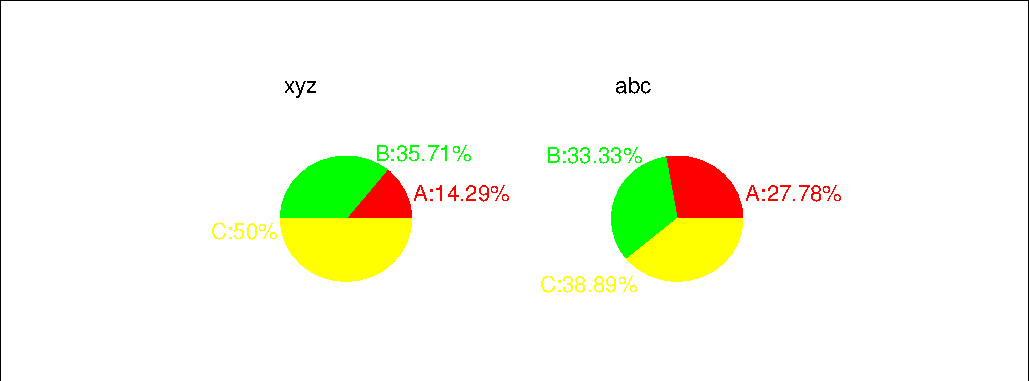
\includegraphics[width=\textwidth]{camembert}\end{center}
\section{Les fonctions statistiques \`a 2 variables}
On continue \`a utiliser la liste {\tt A} dans les exemples.\\
On tape :\\
\begin{center}{\tt A:=[0,1,2,3,4,5,6,7,8,9,10,11]}\end{center}

\subsection{La covariance : {\tt covariance}}\index{covariance}
La covariance de deux variables al\'eatoires
$X$ et $Y$ est :\\
$cov(X,Y)=E((X-\bar X)(Y-\bar Y))$.\\
{\tt covariance} a diff\'erentes sortes d'arguments :

- quand les effectifs sont \'egaux \`a 1,\\
 {\tt covariance} a pour argument deux 
listes de m\^eme longueur ou une matrice ayant deux colonnes.\\
{\tt covariance} calcule la covariance  num\'erique des deux listes ou
deux colonnes de cette matrice.\\
On tape :
\begin{center}{\tt covariance([1,2,3,4],[1,4,9,16])}\end{center}
On obtient :
\begin{center}{\tt  25/4}\end{center}
On tape :
\begin{center}{\tt covariance([[1,1],[2,4],[3,9],[4,16]])}\end{center}
On obtient :
\begin{center}{\tt  25/4}\end{center}
Car on a :\\
1/4*(1+8+27+64)-75/4=25/4\\
On tape (on a {\tt A:=[0,1,2,3,4,5,6,7,8,9,10,11]}) :
\begin{center}{\tt covariance(A,A\verb|^|2)}\end{center}
On obtient :
\begin{center}{\tt 1573/12}\end{center}

- quand les effectifs sont diff\'erents de 1 :\\
- si les couples $a[j],b[j]$ ont pour 
effectif $n[j]$ ($j=0..p-1)$, {\tt covariance} a pour argument 
trois listes $a$, $b$, $n$ de m\^eme longueur $p$, ou 
une matrice de trois colonnes $a$, 
$b$, $n$ et de $p$ lignes $[a[j],b[j],n[j]]$.\\ 
{\tt covariance} calcule la covariance  num\'erique 
des deux premi\`eres listes pond\'er\'ees par la liste donn\'ee comme dernier 
argument ou 
des deux colonnes de cette matrice pond\'er\'ees par la troisi\'eme colonne.\\
On tape :
\begin{center}{\tt covariance([1,2,3,4],[1,4,9,16],[3,1,5,2])}\end{center}
Ou on tape :
\begin{center}{\tt covariance([[1,1,3],[2,4,1],[3,9,5],[4,16,2]])}\end{center}
On obtient :
\begin{center}{\tt 662/121}\end{center}

- si les couples $a[j],b[k]$ ont pour effectif $N[j,k]$ ($j=0..p-1,k=0..q-1$), 
{\tt covariance} a pour argument deux listes $a$, $b$ de longueurs respectives 
$p$ et $q$ et une matrice $N$ de $p$ lignes et $q$ colonnes ou encore,\\
afin de pouvoir \'ecrire les donn\'ees de fa\c{c}on plaisante dans le tableur,
{\tt covariance} peut aussi avoir deux arguments, une matrice $M$ et -1.\\
$M$ est alors un tableau \`a deux entr\'ees \'egal \`a :\\
$$M=\left[\begin{array}{cccc}
a \setminus b & b[0] &...& b[q-1]\\
a[0] & N[0,0] &...& N[0,q-1]\\
...&...&...&...\\
a[p-1] & N[p-1,0] &...& N[p-1,q-1]
\end{array}
\right]
$$
{\tt covariance(a,b,N)} ou  {\tt covariance(M,-1)} calcule la covariance  
num\'erique des couples $a[j],b[k]$  pond\'er\'es par $N_{j,k}$.\\
On tape :
\begin{center}{\tt covariance([1,2,3,4],[1,4,9,16],[[3,0,0,0],}\end{center}
\begin{center}{\tt [0,1,0,0],[0,0,5,0],[0,0,0,2]])}\end{center}
On obtient :
\begin{center}{\tt 662/121}\end{center}
On tape :
\begin{center}{\tt covariance([[b$\setminus$a,1,2,3,4],[1,3,0,0,0],}\end{center}
\begin{center}{\tt [4,0,1,0,0],[9,0,0,5,0],[16,0,0,0,2]],-1)}\end{center}
On obtient :
\begin{center}{\tt 662/121}\end{center}

\subsection{La corr\'elation : {\tt correlation}}\index{correlation}
Le coefficient de corr\'elation lin\'eaire de deux variables al\'eatoires
$X$ et $Y$ est $\displaystyle \rho=\frac{cov(X,Y)}{\sigma(X)\sigma(Y)}$ o\`u 
$\sigma(X)$ (resp $\sigma(Y)$) d\'esigne l'\'ecart-type de $X$ (resp$Y$).\\
{\tt correlation} a les m\^emes arguments que {\tt covariance}.

Quand les effectifs sont \'egaux \`a 1,\\
{\tt correlation} a pour argument deux listes de m\^eme longueur ou une matrice
 ayant deux colonnes.\\
On tape :
\begin{center}{\tt correlation([1,2,3,4],[1,4,9,16])}\end{center}
On obtient :
\begin{center}{\tt 100/(4*sqrt(645))}\end{center}
On tape :
\begin{center}{\tt correlation([[1,1],[2,4],[3,9],[4,16]])}\end{center}
On obtient :
\begin{center}{\tt  100/(4*sqrt(645))}\end{center}
On tape (on a {\tt A:=[0,1,2,3,4,5,6,7,8,9,10,11]}) :
\begin{center}{\tt correlation(A,A\verb|^|2)}\end{center}
On obtient :
\begin{center}{\tt 18876/(572*sqrt(1173))}\end{center}

Quand les effectifs sont diff\'erents de 1 :\\
- si les couples $a[j],b[j]$ ont pour 
effectif $n[j]$ ($j=0..p-1)$, {\tt correlation} a pour argument 
trois listes $a$, $b$, $n$ de m\^eme longueur $p$, ou 
une matrice de trois colonnes $a$, 
$b$, $n$ et de $p$ lignes $[a[j],b[j],n[j]]$.\\ 
{\tt correlation} calcule la corr\'elation num\'erique des deux premi\`eres 
listes qui sont pond\'er\'ees par la liste donn\'ee comme dernier argument ou  
calcule la corr\'elation num\'erique des deux colonnes de cette matrice qui 
sont pond\'er\'ees par la troisi\'eme colonne.\\
On tape :
\begin{center}{\tt correlation([1,2,3,4],[1,4,9,16],[3,1,5,2])}\end{center}
Ou on tape :
\begin{center}{\tt correlation([[1,1,3],[2,4,1],[3,9,5],[4,16,2]])}\end{center}
On obtient :
\begin{center}{\tt  662/(180*sqrt(14))}\end{center}

- si les couples $a[j],b[k]$ ont pour effectif $N[j,k]$ ($j=0..p-1,k=0..q-1$), 
{\tt correlation} a pour argument deux listes $a$, $b$ de longueurs respectives
 $p$ et $q$ et une matrice $N$ de $p$ lignes et $q$ colonnes ou encore,\\
afin de pouvoir \'ecrire les donn\'ees de fa\c{c}on plaisante dans le tableur,
{\tt correlation} peut aussi avoir pour argument, une matrice $M$ et -1.\\
$M$ est alors un tableau \`a deux entr\'ees \'egal \`a :\\
$$M=\left[\begin{array}{cccc}
a \setminus b & b[0] &...& b[q-1]\\
a[0] & N[0,0] &...& N[0,q-1]\\
...&...&...&...\\
a[p-1] & N[p-1,0] &...& N[p-1,q-1]
\end{array}
\right]
$$
{\tt correlation(a,b,N)} ou  {\tt correlation(M,-1)} calcule la corr\'elation  
num\'erique des couples $a[j],b[k]$  pond\'er\'es par $N_{j,k}$.\\
On tape :
\begin{center}{\tt correlation([1,2,3,4],[1,4,9,16],[[3,0,0,0],[0,1,0,0],}\end{center}
\begin{center}{\tt [0,0,5,0],[0,0,0,2]])}\end{center}
On obtient :
\begin{center}{\tt 662/(180*sqrt(14))}\end{center}
On tape :
\begin{center}{\tt correlation([["b$\setminus$a",1,2,3,4],[1,3,0,0,0],}\end{center}
\begin{center}{\tt [4,0,1,0,0],[9,0,0,5,0],[16,0,0,0,2]],-1)}\end{center}
On obtient :
\begin{center}{\tt 662/(180*sqrt(14))}\end{center}

\subsection{Covariance et corr\'elation : {\tt covariance\_correlation}}\index{covariance\_correlation}
\noindent{\tt covariance\_correlation} a les m\^emes arguments que 
{\tt covariance} : si les effectifs sont \'egaux \`a 1,
{\tt covariance\_correlation} a pour argument deux listes de m\^eme longueur ou
 une matrice ayant deux colonnes repr\'esentant deux variables al\'eatoires $X$
et $Y$ et sinon {\tt covariance\_correlation} a pour argument trois listes de 
m\^eme longueur ou une matrice ayant trois colonnes repr\'esentant deux 
variables al\'eatoires $X$ et $Y$ et la pond\'eration de leurs effectifs ou 
encore une matrice $M$ et -1, o\`u $M$ donne la pond\'eration de $X$ (la 
premi\`ere colonne de $M$ sans $M[0,0]$) et de $Y$ (la premi\`ere ligne de $M$
 sans $M[0,0]$).\\
{\tt covariance\_correlation} renvoie la liste de la 
covariance $cov(X,Y)$ et du coefficient de corr\'elation lin\'eaire $\rho$ des
deux variables al\'eatoires $X$ et $Y$.\\
 On a $\rho=\frac{cov(X,Y)}{\sigma(X)\sigma(Y)}$ o\`u
$\sigma(X)$ (resp $\sigma(Y)$) d\'esigne l'\'ecart-type de $X$ (resp$Y$).\\
On tape :
\begin{center}{\tt covariance\_correlation([[1,1],[2,4],[3,9],[4,16]])}\end{center}
On obtient :
\begin{center}{\tt  [25/4,100/(4*sqrt(645))]}\end{center}
On tape (on a {\tt A:=[0,1,2,3,4,5,6,7,8,9,10,11]}) :
\begin{center}{\tt covariance\_correlation(A,A\verb|^|2)}\end{center}
On obtient :
\begin{center}{\tt [1573/12,18876/(572*sqrt(1173))]}\end{center}
On tape :
\begin{center}{\tt covariance\_correlation([1,2,3,4],[1,4,9,16],[3,1,5,2])}\end{center}
Ou on tape :
\begin{center}{\tt covariance\_correlation([[1,1,3],[2,4,1],[3,9,5],[4,16,2]])}\end{center}
On obtient :
\begin{center}{\tt [662/121,662/(180*sqrt(14))]}\end{center}
On tape :
\begin{center}{\tt covariance\_correlation([1,2,3,4],[1,4,9,16],}\end{center}
\begin{center}{\tt [[3,0,0,0],[0,1,0,0],[0,0,5,0],[0,0,0,2]])}\end{center}
On obtient :
\begin{center}{\tt [662/121,662/(180*sqrt(14))]}\end{center}
On tape :
\begin{center}{\tt covariance\_correlation([["b$\setminus$a",1,2,3,4],[1,3,0,0,0], [4,0,1,0,0],[9,0,0,5,0],[16,0,0,0,2]],-1)}\end{center}
On obtient :
\begin{center}{\tt [662/121,662/(180*sqrt(14))]}\end{center}

\subsection{Le nuage de points : {\tt scatterplot nuage\_points}}\index{scatterplot}\index{nuage\_points}
\noindent{\tt scatterplot} ou {\tt nuage\_points} a pour arguments deux listes 
ou une matrice ayant deux colonnes.\\
{\tt scatterplot}  ou {\tt nuage\_points} permet de visualiser le nuage de 
points d\'efini par l'argument.\\
On tape :
\begin{center}{\tt scatterplot([[0,0],[1,1],[2,4],[3,9],[4,16]])}\end{center}
Ou on tape :
\begin{center}{\tt scatterplot([0,0],[1,1],[2,4],[3,9],[4,16])}\end{center}
Ou on tape :
\begin{center}{\tt scatterplot([0,1,2,3,4],[0,1,4,9,16])}\end{center}
La fen\^etre graphique s'ouvre automatiquement et on obtient le dessin des 
 5 points ((0,0),...(4,16)), \`a condition d'avoir d\'efini correctement
la configuration du graphique (menu {\tt Cfg}).

\subsection{Les batons du nuage de points : {\tt batons}}\index{batons}
\noindent{\tt batons} a pour arguments deux listes 
ou une matrice ayant deux colonnes.\\
{\tt batons} permet de visualiser les segments qui relient l'axe des $x$ au 
nuage de points d\'efini par l'argument.\\
On tape :
\begin{center}{\tt batons([[0,0],[1,1],[2,4],[3,9],[4,16]])}\end{center}
Ou on tape :
\begin{center}{\tt batons([0,0],[1,1],[2,4],[3,9],[4,16])}\end{center}
Ou on tape :
\begin{center}{\tt batons([0,1,2,3,4],[0,1,4,9,16])}\end{center}
La fen\^etre graphique s'ouvre automatiquement et on obtient le dessin des 5
segments verticaux reliant l'axe des $x$ aux 5 points ((0,0),...(4,16)), 
\`a condition d'avoir d\'efini correctement
la configuration du graphique (menu {\tt Cfg}).

\subsection{Ligne polygonale : {\tt polygonplot ligne\_polygonale}}\index{polygonplot}\index{ligne\_polygonale}
\noindent{\tt polygonplot} a pour arguments deux listes ou une matrice 
ayant deux colonnes.\\
{\tt polygonplot} permet de visualiser les segments de droites reliant les 
diff\'erents points du nuage de points d\'efinis  par 
l'argument et ordonn\'es selon les abscisses croissantes. Si vous voulez que 
les points soient reli\'es dans l'ordre donn\'es il faut utiliser 
{\tt listplot}\\ 
On tape :
\begin{center}{\tt polygonplot([[0,0],[1,1],[2,4],[3,9],[4,16]])}\end{center}
Ou on tape car les points seront ordonn\'es selon les abscisses croissantes :
\begin{center}{\tt polygonplot([[2,4],[0,0],[3,9],[1,1],[4,16]])}\end{center}
Ou on tape :
\begin{center}{\tt polygonplot([0,1,2,3,4],[0,1,4,9,16])}\end{center}
La fen\^etre graphique s'ouvre automatiquement et on obtient le dessin des 
4 segments reliant les 5 points ((0,0),...(4,16)), 
\`a condition d'avoir d\'efini correctement
la configuration du graphique (menu {\tt Cfg}).

\subsection{Ligne polygonale : {\tt listplot plotlist}}\index{listplot}\index{plotlist}
\noindent{\tt listplot} ou {\tt plotlist} a pour argument une liste {\tt l} ou 
une matrice ayant deux colonnes.\\
{\tt listplot} ou {\tt plotlist} permet de visualiser les segments reliant le 
nuage de points ayant 
pour abscisse {\tt [0,1,2...n]} et pour ordonn\'ee {\tt l} ou pour coordonn\'ees
une ligne de la matrice. {\tt listplot} ou {\tt plotlist} relie par des 
segments de droites, les diff\'erents points du nuage, mais sans r\'eordonner 
les points contrairement \`a {\tt polygonplot} qui  r\'eordonne les points 
selon leur abscisse puis les relie.\\ 
On tape :
\begin{center}{\tt listplot([0,1,4,9,16])}\end{center}
Ou on tape :
\begin{center}{\tt listplot([[0,0],[1,1],[2,4],[3,9],[4,16]])}\end{center}
La fen\^etre graphique s'ouvre automatiquement et on obtient \`a condition d'avoir d\'efini correctement la configuration du graphique (menu {\tt Cfg}) :
 \begin{center}{\tt le dessin des 5 points ((0,0),(1,1),...(4,16)) reli\'es par 4 segments}\end{center} 
On tape si $A$ est une matrice ayant 5 lignes et 2 colonnes :
\begin{center}{\tt A:=[[0,0],[1,1],[5,4],[3,9],[4,16]]}\end{center} 
\begin{center}{\tt listplot(A[0..4,0..1])}\end{center}
La fen\^etre graphique s'ouvre automatiquement et on obtient :
\begin{center}{\tt les 5 points reli\'es par 4 segments}\end{center} 
{\bf Bien voir} la diff\'erence entre :
 \begin{center}{\tt listplot([[0,0],[1,1],[5,4],[3,9],[4,16]])}\end{center}
\begin{center}{\tt polygonplot([[0,0],[1,1],[5,4],[3,9],[4,16]])}\end{center}
{\bf Attention} \\
{\tt listplot([0,1,2,3,4],[0,1,4,9,16])} ou\\ 
{\tt listplot([[0,1,2,3,4],[0,1,4,9,16]])} n'est pas valide !

\subsection{Ligne polygonale et nuage de points : {\tt polygonscatterplot ligne\_polygonale\_pointee}}\index{polygonscatterplot}\index{ligne\_polygonale\_pointee}
\noindent{\tt polygonscatterplot} ou {\tt  ligne\_polygonale\_pointee} a pour 
arguments deux listes ou une matrice ayant deux colonnes.\\
{\tt polygonscatterplot} ou {\tt  ligne\_polygonale\_pointee} permet de 
visualiser le nuage de points d\'efini par 
l'argument, en reliant par des segments de droites, les diff\'erents points du
 nuage en les ordonnant selon les abscisses croissantes.\\
On tape :
\begin{center}{\tt polygonscatterplot([[0,0],[1,1],[2,4],[3,9],[4,16]])}\end{center}
Ou on tape :
\begin{center}{\tt polygonscatterplot([0,1,2,3,4],[0,1,4,9,16])}\end{center}
La fen\^etre graphique s'ouvre automatiquement et on obtient le dessin des 
5 points ((0,0),...(4,16)) reli\'es par 4 segments, 
\`a condition d'avoir d\'efini correctement
la configuration du graphique (menu {\tt Cfg}).

\subsection{Interpolation lin\'eaire : {\tt linear\_interpolate}}\index{linear\_interpolate}
\'E tant donn\'e  une matrice \`a 2 lignes donnant
les coordonn\'ees de points : apres avoir ordonn\'e les abcisses de ces points,
ces points d\'efinissent une ligne polygonale.
On veut avoir les coordonn\'ees des points de cette ligne pour des points
 d\'efinis de maniere r\'eguli\`ere.\\
{\tt linear\_interpolate} a 4 arguments, une matrice {\tt A} \`a 2 lignes donnant
les coordonn\'ees des points d'une ligne polygonale, la valeur minimum des x 
({\tt xmin}), la valeur maximum des x ({\tt xmax}) et le pas ({\tt xstep}).\\
{\tt linear\_interpolate} renvoie les coordonn\'ees des points de la ligne 
polygonale pour x variant de {\tt xmin} \`a {\tt xmax} avec un pas \`egal \`a 
{\tt xstep}.\\
{\bf Remarque} on doit avoir {\tt xmin} et {\tt xmax} dans l'intervalle 
{\tt [min(A[0]);max(A[0])]}.\\
On tape :
\begin{center}{\tt linear\_interpolate([[1,2,6,9],[3,4,6,12]],1,9,1)}\end{center}
On obtient :
\begin{center}{\tt [[1.0,2.0,3.0,4.0,5.0,6.0,7.0,8.0,9.0],[3.0,4.0,4.5,5.0,5.5,6.0,8.0,10.0,12.0]]}\end{center}
On tape :
\begin{center}{\tt linear\_interpolate([[1,2,6,9],[3,4,6,12]],2,7,1)}\end{center}
On obtient :
\begin{center}{\tt [[2.0,3.0,4.0,5.0,6.0,7.0],[4.0,4.5,5.0,5.5,6.0,8.0]]}\end{center}
On tape :
\begin{center}{\tt linear\_interpolate([[1,2,9,6],[3,4,6,12]],1,9,1)}\end{center}
On obtient :
\begin{center}{\tt [[1.0,2.0,3.0,4.0,5.0,6.0,7.0,8.0,9.0],[3.0,4.0,6.0,8.0,10.0,12.0,10.0,8.0,6.0]]}\end{center}

\subsection{R\'egression lin\'eaire : {\tt linear\_regression}}\index{linear\_regression}
Pour approcher les donn\'ees  par la droite des moindres carr\'es ayant pour
\'equation $y=mx+b$, on utilise  {\tt linear\_regression} qui renvoie le couple
 $(m,b)$.\\
Si les donn\'ees sont $x_i,y_i$ avec $i=1..n$, on a :\\
$m=\frac{cov(X,Y)}{\sigma(X)^2}$\\
et $b=\bar{Y}-m\bar{X}$\\
 car la somme des carr\'es des distances $d_i=|y_i-mx_i-b_i|$ est 
minimale pour ces valeurs et ce minimum (qui est donc l'erreur quadratique 
moyenne verticale) vaut $(1-\rho^2)\sigma(Y)^2$ o\`u $r$ est
le coefficient de corr\'elation ($\rho=\frac{cov(X,Y}{\sigma(X)\sigma(Y)}$).\\
{\tt linear\_regression} a les m\^emes arguments que {\tt covariance}.\\
On tape :
\begin{center}{\tt linear\_regression([[0,0],[1,1],[2,4],[3,9],[4,16]])}\end{center}
Ou on tape :
\begin{center}{\tt linear\_regression([0,1,2,3,4],[0,1,4,9,16])}\end{center}
On obtient :
\begin{center}{\tt 4,-2}\end{center}
c'est donc la fonction lin\'eaire d'\'equation $y=4x-2$ 
qui approche au mieux les donn\'ees.\\
On tape :
\begin{center}{\tt X:=[0,1,2,3,4,5,6,7,8,9,10]}\end{center}
\begin{center}{\tt Y:=[7.3,9.53,12.47,16.3,21.24,27.73,36.22,}\end{center}
\begin{center}{\tt 47.31,61.78,80.68,105]}\end{center}
\begin{center}{\tt Z:=log(Y)}\end{center}
\begin{center}{\tt linear\_regression(X,Z)}\end{center}
On obtient :
\begin{center}{\tt 0.266729219953,1.98904252589}\end{center}
c'est donc la fonction lin\'eaire d'\'equation $z=\ln(y)=0.267x+1.99$ 
qui approche au mieux les donn\'ees.

\subsection{Graphe de la r\'egression lin\'eaire :\\ 
{\tt linear\_regression\_plot}}\index{linear\_regression\_plot}\index{equation@{\sl equation}|textbf}\index{correlation@{\sl correlation}|textbf}
Pour dessiner la droite des moindres carr\'es $y=mx+b$, droite qui approche au 
mieux les donn\'ees, on utilise  {\tt linear\_regression\_plot}.\\
{\tt linear\_regression\_plot} a les m\^emes arguments que {\tt covariance}.\\
On tape :
\begin{center}{\tt linear\_regression\_plot([1,2,3,4],[1,4,9,16],[3,1,5,2])}\end{center}
On obtient :
\begin{center}{\tt Le graphe de la droite d'\'equation $y=331*x/70-22/5$}\end{center}
car c'est la fonction lin\'eaire d'\'equation $y=331*x/70-22/5$ qui approche au
 mieux les donn\'ees.
{\bf Remarque}
On remarquera que l'\'equation de la courbe represent\'ee ainsi que la valeur 
du coefficient de corr\'elation des donn\'ees sont \'ecrits en bleu.\\
Si on veut avoir l'\'equation et/ou le coefficient de corr\'elation  sur le 
dessin il faut rajouter comme dernier argument, l'option {\tt equation} et/ou 
{\tt correlation}.

\subsection{R\'egression exponentielle : {\tt exponential\_regression}}\index{exponential\_regression}
Pour approcher les donn\'ees par une fonction exponnentielle d'\'equation 
$y=be^{mx}=ba^x$, on utilise  {\tt exponential\_regression} qui 
renvoie le couple $(a,b)$.\\
{\tt exponential\_regression} a les m\^emes arguments que {\tt covariance}.\\
On tape :
\begin{center}{\tt evalf(exponential\_regression([[1,1],[2,4],[3,9],[4,16]]))}\end{center}
Ou on tape :
\begin{center}{\tt evalf(exponential\_regression([1,2,3,4],[1,4,9,16]))}\end{center}
On obtient :
\begin{center}{\tt  2.49146187923,0.5}\end{center}
c'est donc la fonction exponentielle d'\'equation $y=0.5*(2.49146187923)^x$
qui approche au mieux les donn\'ees.\\
On tape :
\begin{center}{\tt X:=[0,1,2,3,4,5,6,7,8,9,10]}\end{center}
\begin{center}{\tt Y:=[7.3,9.53,12.47,16.3,21.24,27.73,36.22,47.31,}\end{center}
\begin{center}{\tt 61.78,80.68,105]}\end{center}
\begin{center}{\tt exponential\_regression(X,Y)}\end{center}
On obtient :
\begin{center}{\tt 1.30568684451,7.30853268031}\end{center}
c'est donc la fonction exponentielle d'\'equation $y=7.3*(1.3)^x$ 
qui approche au mieux les donn\'ees.
On v\'erifie en tapant :\\
\begin{center}{\tt e\verb|^|[linear\_regression(X,ln(Y))]}\end{center}
On obtient :
\begin{center}{\tt 1.30568684451,7.30853268031}\end{center}

\subsection{Graphe de la r\'egression exponentielle : \\
{\tt exponential\_regression\_plot}}\index{exponential\_regression\_plot}\index{equation@{\sl equation}}\index{correlation@{\sl correlation}}
Pour dessiner la fonction exponnentielle d'\'equation $y=b\exp(mx)=ba^x$ qui 
approche au mieux les donn\'ees, on utilise  {\tt exponential\_regression\_plot}.\\
 {\tt exponential\_regression\_plot} a  les m\^emes arguments que {\tt covariance}.\\
On tape  :
\begin{center}{\tt exponential\_regression\_plot([0,1,2,3,4,5,6,7,8,9,10],[7.3, 9.53,12.47,16.3,21.24,27.73,36.22,47.31,61.78,80.68,105])}\end{center}
On obtient :
\begin{center}{\tt Le graphe de la fonction expopnentielle d'\'equation $y=7.30853268031*(1.30568684451)^x$}\end{center}
car c'est la fonction expopnentielle d'\'equation :\\
$y=7.30853268031*(1.30568684451)^x$ qui approche au mieux les donn\'ees.
{\bf Remarque}
On remarquera que l'\'equation de la courbe represent\'ee ainsi que la valeur 
du coefficient de corr\'elation de $X,\ln(Y)$ (si les donn\'ees sont $X,Y)$)
sont \'ecrits en bleu.\\
Si on veut avoir l'\'equation et/ou le coefficient de corr\'elation  sur le 
dessin il faut rajouter comme dernier argument, l'option {\tt equation} et/ou 
{\tt correlation}.

\subsection{R\'egression logarithmique : {\tt logarithmic\_regression}}\index{logarithmic\_regression}
Pour approcher les donn\'ees par une fonction logarithmique d'\'equation 
$y=m\ln(x)+b$, on utilise  {\tt logarithmic\_regression} qui renvoie le couple 
$(m,b)$.\\
{\tt logarithmic\_regression} a les m\^emes arguments que {\tt covariance}.\\
On tape :
\begin{center}{\tt evalf(logarithmic\_regression([[1,1],[2,4],[3,9],[4,16]]))}\end{center}
Ou on tape :
\begin{center}{\tt evalf(logarithmic\_regression([1,2,3,4],[1,4,9,16]))}\end{center}
On obtient :
\begin{center}{\tt  10.1506450002,-0.564824055818}\end{center}
c'est donc la fonction logarithmique d'\'equation 
$y=10.15\ln(x)-0.565$ qui approche au mieux les donn\'ees.\\
On tape :
\begin{center}{\tt X:=[1,1.5,2,2.5,3,3.5,4,4.5,5,5.5,6,6.5,7,7.5,8]}\end{center}
\begin{center}{\tt Y:=[1.6,2.15,2.65,3.12,3.56,3.99,4.4,4.8,5.18,}\end{center}
\begin{center}{\tt 5.58,5.92,6.27,6.62,7.06,7.3]}\end{center}
\begin{center}{\tt logarithmic\_regression(X,Y)}\end{center}
On obtient :
\begin{center}{\tt  2.83870854646,0.843078064152}\end{center}
c'est donc la fonction logarithmique d'\'equation 
$y=0.84\ln(x)+2.84$ qui approche au mieux les donn\'ees .\\
On v\'erifie en tapant :\\
\begin{center}{\tt linear\_regression(ln(X),Y)}\end{center}
On obtient :
\begin{center}{\tt  2.83870854646,0.843078064152}\end{center}
et le coefficient de corr\'elation est :
\begin{center}{\tt correlation(ln(X),Y)}\end{center}
On obtient :
\begin{center}{\tt  0.977939822434}\end{center}
On peut aussi taper pour chercher une meilleur approximation :
\begin{center}{\tt logarithmic\_regression(X,log(Y))}\end{center}
On obtient :
\begin{center}{\tt  0.732351031846,0.467599676658}\end{center}
c'est donc la fonction logarithmique d'\'equation 
$z=\ln(y)=0.73\ln(x)+0.47$ qui approche au mieux les donn\'ees.\\
On v\'erifie en tapant :\\
\begin{center}{\tt linear\_regression(ln(X),ln(Y))}\end{center}
On obtient :
\begin{center}{\tt  0.732351031846,0.467599676658}\end{center}
et le coefficient de corr\'elation est :
\begin{center}{\tt correlation(ln(X),ln(Y))}\end{center}
On obtient :
\begin{center}{\tt  0.999969474543}\end{center}

\subsection{Graphe de la r\'egression logarithmique : \\
{\tt logarithmic\_regression\_plot}}\index{logarithmic\_regression\_plot}\index{equation@{\sl equation}}\index{correlation@{\sl correlation}}
Pour dessiner le graphe de la fonction logarithmique d'\'equation 
$y=m \ln x+b$ qui approche au mieux  les donn\'ees, on utilise  
{\tt logarithmic\_regression\_plot}.\\
{\tt logarithmic\_regression\_plot} a les m\^emes arguments que {\tt covariance}.\\
On tape :
\begin{center}{\tt logarithmic\_regression\_plot([[1.0,1],[2,4],[3,9],[4,16]])}\end{center}
On obtient :
\begin{center}{\tt Le graphe de la fonction logarithme d'\'equation $y=10.1506450002\ln(x)-0.564824055818$}\end{center}
car c'est la fonction logarithme d'\'equation :\\
$y=10.1506450002\ln(x)-0.564824055818$ \\
qui approche au mieux les donn\'ees.\\
{\bf Remarque}
On remarquera que l'\'equation de la courbe represent\'ee ainsi que la valeur 
du coefficient de corr\'elation de $\ln(X),\ln(Y)$ (si les donn\'ees sont 
$X,Y)$) sont \'ecrits en bleu.\\
Si on veut avoir l'\'equation et/ou le coefficient de corr\'elation  sur le 
dessin il faut rajouter comme dernier argument, l'option {\tt equation} et/ou 
{\tt correlation}.

\subsection{R\'egression polyn\^omiale : {\tt polynomial\_regression}}\index{polynomial\_regression}
Pour approcher les donn\'ees par une fonction polyn\^omiale de degr\'e $\leq n$
d'\'equation $y=a_0x^n+..+a_n$, on utilise, en mettant le degr\'e $n$ comme 
dernier param\`etre, {\tt polynomial\_regression} qui renvoie la liste 
$[a_n,..a_0]$.\\
{\tt polynomial\_regression} a les m\^emes premiers arguments que 
{\tt covariance}, le dernier argument \'etant le degr\'e du polyn\^ome 
renvoy\'e.\\
On tape :
\begin{center}{\tt polynomial\_regression([[1,1],[2,4],[3,9],[4,16]],3)}\end{center}
Ou on tape :
\begin{center}{\tt polynomial\_regression([1,2,3,4],[1,4,9,16],3)}\end{center}
On obtient :
\begin{center}{\tt [0,1,0,0]}\end{center}
c'est donc la fonction polynomiale d'\'equation $y=0*x^3+x^2+0*x+0=x^2$ 
qui approche au mieux les donn\'ees.
{\bf Remarque}
On remarquera que l'\'equation de la courbe represent\'ee ainsi que la valeur 
du coefficient de corr\'elation des donn\'ees sont \'ecrits en bleu.\\
Si on veut avoir l'\'equation et/ou le coefficient de corr\'elation  sur le 
dessin il faut rajouter comme dernier argument, l'option {\tt equation} et/ou 
{\tt correlation}.

\subsection{Graphe de la r\'egression polynomiale :\\
 {\tt polynomial\_regression\_plot}}\index{polynomial\_regression\_plot}
Pour approcher les donn\'ees par le grahe d'une fonction polyn\^omiale de 
degr\'e $\leq n$ d'\'equation $y=a_0x^n+..+a_n$, on utilise  
{\tt polynomial\_regression\_plot}.\\
{\tt polynomial\_regression\_plot} a les m\^emes premiers arguments que 
{\tt covariance}, le dernier argument \'etant le degr\'e du polyn\^ome 
renvoy\'e.\\
On tape :
\begin{center}{\tt polynomial\_regression\_plot([[1.0,1],[2,4],[3,9],[4,16]],3)}\end{center}
On obtient :
\begin{center}{\tt Le graphe de la fonction polyn\^omiale de degr\'e $\leq n$ d'\'equation $y=x^2$}\end{center}
car c'est la fonction polyn\^omiale d'\'equation $y=1*x^2$ qui approche au 
mieux les donn\'ees.

\subsection{R\'egression puissance : {\tt power\_regression}}\index{power\_regression}
Pour approcher les donn\'ees par une fonction puissance d'\'equation
$y=bx^m$, on utilise  {\tt power\_regression} qui renvoie le couple $(m,b)$.\\
{\tt power\_regression} a les m\^emes arguments que {\tt covariance}.\\
On tape :
\begin{center}{\tt evalf(power\_regression([[1,1],[2,4],[3,9],[4,16]]))}\end{center}
Ou on tape :
\begin{center}{\tt evalf(power\_regression([1,2,3,4],[1,4,9,16]))}\end{center}
On obtient :
\begin{center}{\tt (2.0,1.0)}\end{center}
donc $y=x^2$  est la fonction puissance qui approche au mieux les donn\'ees.\\
On tape :
\begin{center}{\tt X:=[1,1.5,2,2.5,3,3.5,4,4.5,5,5.5,6,6.5,7,7.5,8]}\end{center}
\begin{center}{\tt Y:=[1.6,2.15,2.65,3.12,3.56,3.99,4.4,4.8,5.18,}\end{center}
\begin{center}{\tt 5.58,5.92,6.27,6.62,7.06,7.3]}\end{center}
\begin{center}{\tt power\_regression(X,Y)}\end{center}
On obtient :
\begin{center}{\tt  0.732351031846,1.59615829535}\end{center}
c'est donc la fonction puissance d'\'equation 
$y=1.6*x^{0.73}$ qui approche au mieux les donn\'ees.\\
On v\'erifie en tapant :\\
\begin{center}{\tt linear\_regression(ln(X),ln(Y))}\end{center}
On obtient :
\begin{center}{\tt  0.732351031846,0.467599676658}\end{center}
On a bien :\\
\begin{center}{\tt  e\verb|^|0.467599676658=1.59615829535}\end{center}
donc \\
$\ln(y)=\ln(1.59615829535)+\ln(x)*0.732351031846$\\
$\ln(y)=0.467599676659+\ln(x)*0.732351031846$.
et le coefficient de corr\'elation est :
\begin{center}{\tt correlation(ln(X),ln(Y))}\end{center}
On obtient :
\begin{center}{\tt  0.999969474543}\end{center}

\subsection{Graphe de la r\'egression puissance :\\
 {\tt power\_regression\_plot}}\index{power\_regression\_plot}\index{equation@{\sl equation}}\index{correlation@{\sl correlation}}
Pour approcher les donn\'ees par le graphe d'une fonction puissance 
d'\'equation $y=bx^m$, on utilise  {\tt power\_regression\_plot}.\\
{\tt power\_regression\_plot} a les m\^emes arguments que {\tt covariance}.\\
On tape :
\begin{center}{\tt power\_regression\_plot([[1.0,1],[2,4],[3,9],[4,16]])}\end{center}
On obtient :
\begin{center}{\tt Le graphe de la fonction puissance d'\'equation $y=1*x^2$}\end{center}
car c'est la fonction puissance d'\'equation $y=1*x^2$ qui approche au mieux 
les donn\'ees.
{\bf Remarque}
On remarquera que l'\'equation de la courbe represent\'ee ainsi que la valeur 
du coefficient de corr\'elation des donn\'ees sont \'ecrits en bleu.\\
Si on veut avoir l'\'equation et/ou le coefficient de corr\'elation  sur le 
dessin il faut rajouter comme dernier argument, l'option {\tt equation} et/ou 
{\tt correlation}.

\subsection{R\'egression logistique : {\tt logistic\_regression}}\index{logistic\_regression}
Les courbes logistiques sont des courbes dont l\'equation $y=y(x)$ sont
solutions d'une \'equation diff\'erentielle de la forme :\\
$y'/y=a*y+b$ et $y_0=y(x_0)$ avec $a<0$ et $b>0$.\\
Les solutions sont de la forme : $y(x)=C/(1+\exp(-\alpha (x-x_0-k)$
avec $C=-b/a$, $\alpha=-b$ et $y_0=(-b/a)/(1+\exp(-b*k)$ soit \\
$k=-1/b*(ln(-((a*y0+b)/(a*y0))))$
Pour v\'erifier, on peut taper :
\begin{center}{\tt normal(desolve(y'/y=a*y+b)}\end{center}
On obtient :
\begin{center}{\tt (-b*exp(-(b*c\_0-b*x)))/(a*exp(-(b*c\_0-b*x))-1)}\end{center}Puis on peut taper :
\begin{center}{\tt normal(desolve([y'/y=a*y+b,y(x0)=y0],y)}\end{center}
On obtient :
\begin{center}{\tt [(-b*exp(b*x-b*x0+ln(y0/(a*y0+b))))/(a*exp(b*x-b*x0+ln(y0/(a*y0+b)))-1)]}\end{center}
On a donc :
$c_0=x_0-\ln(y_0/(a*y_0+b))/b$
Donc, en multipliant le num\'erateur et d\'enominateur de $y(x)$ par 
$\exp(b*c\_0-b*x)$ on a :\\
$y(x)=(-b/(\exp(b*c\_0-b*x)*a*exp(-(b*c\_0-b*x))-1)$
soit $y(x)=-b/(a-\exp(b*(x-c_0)))=(-b/(a*(1-\exp(b*(x-c_0))/a))$\\
On a $1/a=-\exp(-ln(-a))$ car $a<0$
donc $y(x)=(-b/a)*(1/(1+\exp(b*(x-c_0)-\ln(-a)))$
qui est bien la forme annonc\'ee.

Lorsque on connait les valeurs de $f'$ en $x=x_0,x_0+1....x_0+n$, on cherche
une fonction logistique $y(x)$ tel que $y'(x)$ approche au mieux les 
diff\'erentes valeurs de $f'(x)$.

{\tt logistic\_regression} a comme param\`etres :
\begin{itemize}
\item une liste {\tt L} qui contient les valeurs de $y'$ pour 
$x=x_0,x_0+1....x_0+n$,
\item la valeur de {\tt x0} de $x_0$
\item la valeur {\tt y0} de $y(x_0)$ lorsqu'on la connait sinon {\tt Xcas}
arrive \`a l'estimer...
\end{itemize}
{\tt logistic\_regression(L,x0,y0} renvoie les fonctions {\tt y(x)} et
{\tt y'(x)}, la constante {\tt C}, {\tt y1M} et {\tt xM} avec {\tt y1M}
est la valeur {\tt y'(xM)} qui est le maximum de $y'$ obtenu en $x=xM$, et 
enfin le coefficient de correlation lin\'eaire {\tt R} de $Y=y'/y$ en fonction 
de $y$ avec la droite $Y=a*y+b$.\\
\`A partir de la liste {\tt L}, {\tt Xcas} calcule la liste {\tt Ly} en 
utilisant la formule $y(t+1)-y(t)=y'(t)$, donc, on a 
{\tt Ly=[y0,y0+y0',y0+y0'+y1',....]}. Puis {\tt Xcas} fait une r\'egression 
lin\'eaire de {\tt L/Ly} en fonction de {\tt Ly} pour avoir les valeurs de 
$a$ et $b$ ($y'/y=a*y+b$ et $y_0=y(x_0)$) puis touve la solution de cette 
\'equation diff\'erentielle 
On tape :
\begin{center}{\tt logistic\_regression([0.0,1.0,2.0,3.0,4.0],0,1)}\end{center}

On obtient avec \'ecrit en bleu la signification des valeurs renvoy\'ees :
\begin{center}{\tt  [(-17.77)/(1+exp(-0.496893925384*x+2.82232341488+3.14159265359*i)), (-2.48542227469)/(1+cosh(-0.496893925384*x+2.82232341488+3.14159265359*i)), -17.77,-1.24271113735,5.67993141131+6.32246138079*i, 0.307024935856] }\end{center}

On tape :
\begin{center}{\tt evalf(logistic\_regression([1,2,4,6,8,7,5],0,2))}\end{center}
Ou on tape :
\begin{center}{\tt logistic\_regression(evalf([1,2,4,6,8,7,5]),0,2.0))}\end{center}
On obtient :
\begin{center}{\tt [64.8358166583/(1.0+exp(-0.551746244591*x+2.95837880348)), 14.4915280084/(1.0+cosh(-0.551746244591*x+2.95837880348)), 64.8358166583,7.24576400418,5.36184674112,-0.81176431297]}\end{center}

Pour retouver la valeur -0.81176431297 du coefficient de corr\'elation, 
on tape :\\
{\tt L:=[1,2,4,6,8,7,5];}\\
{\tt y0:=2.0;}\\
{\tt Ly:=makelist(y0,1,size(L))+cumSum(L)}\\
On obtient :
{\tt [3,5,9,15,23,30,35]}\\
puis \\
{\tt correlation(L/Ly,Ly)} qui renvoie\\
{\tt -0.81176431297}
\subsection{Graphe de la r\'egression logistique :\\
 {\tt logistic\_regression\_plot}}\index{logistic\_regression\_plot}\index{equation@{\sl equation}}\index{correlation@{\sl correlation}}
Lorsque on connait les valeurs de $f'(x)$ en $x=x_0,x_0+1....x_0+n$, pour 
tracer le graphe de la deriv\'ee $y'(x)$ d'une fonction logistique $y(x)$, 
solution de l'\'equation 
$y'/y=a*y+b$ ($a<0$ et $b>0$) v\'erifiant $y_0=y(x_0)$ et tel que $y'(x)$ 
approche au mieux  les diff\'erentes valeurs de $f'(x)$, on utilise  
{\tt logistic\_regression\_plot}.\\
{\tt logistic\_regression\_plot} a les m\^emes arguments que 
{\tt logistic\_regression}.\\
On tape :
\begin{center}{\tt logistic\_regression\_plot([1,2,4,6,8,7,5],0,2.0)}\end{center}
On obtient avec \'ecrit en bleu les valeurs renvoy\'ees par:
\begin{center}{\tt Le graphe de la fonction solution de $y'/y=a*y+b$ avec $y'(0)=1,y'(1)=2,y'(3)=4...y'(6)=5$, $y(0)=2$}\end{center}
car c'est la fonction logistique qui approche au mieux les donn\'ees.
{\bf Remarque}
On remarquera que l'\'equation de la courbe represent\'ee ainsi que la valeur 
du coefficient de corr\'elation des donn\'ees sont \'ecrits en bleu.\\
Si on veut avoir l'\'equation et/ou le carr\'e du coefficient de corr\'elation 
sur le dessin il faut rajouter comme dernier argument, l'option {\tt equation} 
et/ou {\tt correlation}. Par exemple,
 {\tt logistic\_regression\_plot([1,2,4,6,8,7,5],0,2.0,correlation)}
et {\tt R2=0.658961299812} s'inscrit sur le graphe.

\section{Les fonctions al\'eatoires de {\tt Xcas}}
\subsection{Pour initialiser les nombres al\'eatoires : {\tt srand randseed RandSeed}}\index{srand}\index{randseed}\index{RandSeed}
\noindent{\tt srand} (ou {\tt randseed} ou {\tt RandSeed})  sert \`a 
initialiser la suite des nommbres al\'eatoires que l'on obtient avec 
{\tt rand()} ou avec {\tt randnorm()}.\\
{\tt RandSeed} a toujours un argument entier, alors que {\tt randseed} ou 
{\tt srand} peut ne pas avoir d'arguments (dans ce cas le g\'en\'erateur 
al\'eatoire est intialis\'e avec l'horloge du syst\`eme).\\ 
Ainsi, {\tt srand(n)} (ou {\tt randseed(n)} ou {\tt RandSeed(n)}) avec {\tt n} 
entier sert \`a initialiser la suite des nommbres al\'eatoires pour que l'on 
puisse obtenir la m\^eme suite al\'eatoire avec {\tt rand()} ou avec 
{\tt randnorm()}.\\
On tape :
\begin{center}{\tt srand}\end{center}
On obtient par exemple :
\begin{center}{\tt 1054990506}\end{center}
On tape :
\begin{center}{\tt srand(121054990506)}\end{center}
On obtient  :
\begin{center}{\tt 121054990506}\end{center}
Ou on tape :
\begin{center}{\tt  RandSeed(10549905061234)}\end{center}
On obtient par exemple :
\begin{center}{\tt 10549905061234}\end{center}

\subsection{Tirage \'equir\'eparti {\tt rand alea hasard}}\index{rand|textbf}\index{hasard|textbf}\index{alea|textbf}
\subsubsection{Tirage \'equir\'eparti sur $[0,1[$ : {\tt rand() alea() hasard}}
\noindent{\tt rand()} renvoie au hasard, de façon \'equiprobable, un nombre 
r\'eel de $[0,1[$.\\
On tape :
\begin{center}{\tt rand()}\end{center}
ou on tape
\begin{center}{\tt alea()}\end{center}
ou on tape (attention {\tt hasard} n'utilise pas de {\tt ()} et est utilis\'e 
pour le langage de la tortue)
\begin{center}{\tt hasard}\end{center}
On obtient par exemple:
\begin{center}{\tt 0.912569261115}\end{center}
Pour avoir, au hasard, de façon \'equiprobable, un nombre de $[0;1[$, on peut 
aussi utiliser (voir le paragraphe suivant):
\begin{center}{\tt rand(0,1)}\end{center}
On obtient :
\begin{center}{\tt 0.391549611697}\end{center}

\subsubsection{Tirage al\'eatoire \'equir\'eparti sur l'intervalle [a;b[ : {\tt rand(a,b) hasard(a,b) rand(a..b)() hasard(a..b)()}}
Si {\tt a} et {\tt b} sont des r\'eels {\tt rand(a,b)} d\'esigne un nombre 
d\'ecimal al\'eatoire compris dans l'intervalle $[a;b[$.\\
Donc, {\tt rand(a,b)} ou ({\tt hasard(a,b)}) renvoie au hasard, et de façon 
\'equiprobable, un nombre d\'ecimal de $[a;b[$.\\
Pour avoir, au hasard et de façon \'equiprobable, un nombre d\'ecimal de $[0;1[$, 
on tape :
\begin{center}{\tt rand(0,1)}\end{center}
On obtient :
\begin{center}{\tt 0.391549611697}\end{center}
ou on tape (attention {\tt hasard} utilise des {\tt ()} qui englobent hasard et sesparam\`etres et {\tt hasard} est 
utilis\'e pour le langage de la tortue)
\begin{center}{\tt (hasard 0,1)}\end{center}
On obtient par exemple:
\begin{center}{\tt 0.912569261115}\end{center}
Pour avoir, au hasard et de façon \'equiprobable, un nombre d\'ecimal de 
$[0;0.5[$, on tape :
\begin{center}{\tt rand(0,0.5)}\end{center}
On obtient :
\begin{center}{\tt 0.303484437987}\end{center}
Pour avoir, au hasard et de façon \'equiprobable, un nombre d\'ecimal de $]-0.5;0]$, 
on tape :
\begin{center}{\tt rand(0,-0.5)}\end{center}
ou on tape :
\begin{center}{\tt rand(-0.5,0)}\end{center}
On obtient par exemple :
\begin{center}{\tt -0.20047219703}\end{center}

Si {\tt a} et {\tt b} sont des r\'eels {\tt rand(a..b)} ou {\tt alea(a..b)} ou 
{\tt hasard(a..b)} d\'esigne une fonction qui est un  g\'en\'erateur de nombres
al\'eatoires compris dans l'intervalle $[a;b[$.\\
Donc, {\tt rand(a..b)()} renvoie au hasard, et de façon \'equiprobable, un
 nombre d\'ecimal de $[a;b[$.\\
Pour avoir, au hasard et de façon \'equiprobable, un nombre d\'ecimal de $[0;1[$, 
on tape :
\begin{center}{\tt rand(0..1)()}\end{center}
On obtient :
\begin{center}{\tt  0.391549611697}\end{center}
Pour avoir, au hasard et de façon \'equiprobable, plusieurs nombres 
al\'eatoires d\'ecimaux compris dans l'intervalle $[1;2[$, 
on tape :
\begin{center}{\tt r:=rand(1..2)}\end{center}
puis il suffit de taper {\tt r()}.\\
On tape :
\begin{center}{\tt r()}\end{center}
On obtient :
\begin{center}{\tt 1.14160255529}\end{center}

\subsubsection{Tirage al\'eatoire d'entiers \'equir\'epartis sur $[0,..,n[$ : {\tt rand(n) alea(n) hasard(n)}}\index{rand}\index{hasard}\index{alea}
Si {\tt n} est un entier relatif {\tt rand(n)} ou {\tt hasard(n)} renvoie au 
hasard, et de façon \'equiprobable, un entier de $[0,1,..,n[$ 
(ou de $]n,..1,0]$ si $n$ est negatif).\\
On tape :
\begin{center}{\tt rand(2)}\end{center}
Ou on tape :
\begin{center}{\tt alea(2)}\end{center}
Ou on tape :
\begin{center}{\tt hasard(2)}\end{center}
ou
\begin{center}{\tt hasard 2}\end{center}
On obtient :
\begin{center}{\tt  1}\end{center}
ou on obtient :
\begin{center}{\tt  0}\end{center}
On tape :
\begin{center}{\tt rand(-2)}\end{center}
Ou on tape :
\begin{center}{\tt hasard(-2)}\end{center}
On obtient :
\begin{center}{\tt  -1}\end{center}
ou on obtient :
\begin{center}{\tt  0}\end{center}
On tape pour avoir un entier al\'eatoire entre 6 et 10, bornes comprises :
\begin{center}{\tt 6+rand(11-6)}\end{center}
Ou on tape :
\begin{center}{\tt 6+hasard(11-6)}\end{center}
On obtient par exemple :
\begin{center}{\tt  8}\end{center}

\subsubsection{Tirage al\'eatoire sans remise de p objets parmi n : {\tt rand alea hasard}}\index{rand}\index{hasard}\index{alea}
{\tt rand} a dans ce cas, soit 2, soit  3 arguments.\\
 Si {\tt rand} a  2 arguments : les arguments sont un entier $p$ et une liste 
$L$ alors {\tt rand(p,L)} renvoie, au hasard, {\tt p} \'el\'ements de la liste 
{\tt L}.\\
 Si  {\tt rand} a  3 arguments : les arguments sont trois entiers 
{\tt p,min,max} alors
{\tt rand(p,min,max)} renvoie, au hasard, {\tt p} entiers de  
{\tt [min,..,max]} 
On tape :
\begin{center}{\tt rand(3,["r","r","r","r","v","v","v"])}\end{center}
On obtient :
\begin{center}{\tt  ["r","r","v"]}\end{center}
On tape :
\begin{center}{\tt rand(2,1,10)}\end{center}
On obtient :
\begin{center}{\tt  [3,7]}\end{center}
On tape :
\begin{center}{\tt rand(2,4,10)}\end{center}
On obtient :
\begin{center}{\tt [5,7]}\end{center}

\subsection{Tirage selon une loi binomiale : {\tt randbinomial}}\index{randbinomial}
\noindent{\tt randbinomial(n,p)} renvoie au hasard des nombres entiers 
r\'epartis selon la loi binomiale $B(n,p)$ de moyenne {\tt n*p} et d'\'ecart 
type {\tt sqrt(n*p*(1-p))}.\\
{\tt randbinomial(n,p)} a pour valeur le nombre de succ\`es dans une suite de 
{\tt n} tirages ind\'ependants lorsque pour chaque tirage, un succ\`es est de 
probabilit\'e {\tt p}.\\
On tape :
\begin{center}{\tt randbinomial(10,0.6)}\end{center}
On obtient par exemple :
\begin{center}{\tt 4}\end{center}
ou on obtient par exemple :
\begin{center}{\tt  8}\end{center}
On tape :
\begin{center}{\tt randbinomial(100,0.4)}\end{center}
On obtient par exemple :
\begin{center}{\tt 43}\end{center}
\subsection{Tirage selon une loi multinomiale : {\tt randmultinomial}}\index{randmultinomial}
\noindent{\tt randmultinomial(P)} renvoie un index ou {\tt randmultinomial(P,K)}
renvoie un \'el\'ement de la liste {\tt K}, al\'eatoirement distribu\'e selon 
la loi multinomiale de probabilit\'es donn\'ee par la liste {\tt P}.\\
On tape :
\begin{center}{\tt randmultinomial([1/2,1/3,1/6]}\end{center}
On obtient par exemple :
\begin{center}{\tt 1}\end{center}
Ce qui correspond \`a l'indice de l'objet obtenu avec la probabilit\'e 
{\tt 1/3}.\\
On tape :
\begin{center}{\tt randmultinomial([1/2,1/3,1/6],["R","V","B"])}\end{center}
On obtient par exemple :
\begin{center}{\tt "R"}\end{center}

\subsection{Tirage selon une loi de Poisson : {\tt randpoisson}}\index{randpoisson}
\noindent{\tt randpoisson($\lambda$)} renvoie au hasard des nombres entiers 
r\'epartisselon la loi de Poisson  $P(\lambda)$ de moyenne {\tt $\lambda$} et 
d'\'ecart type {\tt $\sqrt{\lambda}$}.\\
On a :\\
Proba($X\leq k$)=$\exp(-\lambda)\frac{\lambda^k}{k!}$.\\
On tape :
\begin{center}{\tt randpoisson(10.6)}\end{center}
On obtient par exemple :
\begin{center}{\tt 8}\end{center}
ou on obtient par exemple :
\begin{center}{\tt  17}\end{center}
On tape :
\begin{center}{\tt randpoisson(2.4)}\end{center}
On obtient par exemple :
\begin{center}{\tt 1}\end{center}
\subsection{Tirage selon une loi normale : {\tt randnorm randNorm}}\index{randnorm}\index{randNorm}
\noindent {\tt randnorm(m,sigma)} ou {\tt randNorm(m,sigma)} renvoie au hasard 
des nombres r\'epartis selon la loi normale de moyenne {\tt  m} et d'\'ecart 
type {\tt sigma}.\\
On tape :
\begin{center}{\tt randnorm(0,1)}\end{center}
On obtient par exemple :
\begin{center}{\tt 0.549605372982}\end{center}
ou on obtient par exemple :
\begin{center}{\tt  -0.58946494465}\end{center}
On tape :
\begin{center}{\tt randnorm(2,1)}\end{center}
On obtient par exemple :
\begin{center}{\tt 2.54178274488}\end{center}

\subsection{Tirage selon une loi exponentielle : {\tt randexp}}\index{randexp}
\noindent {\tt randexp(a)} renvoie au hasard 
des nombres r\'epartis selon la loi exponentielle de param\`etre {\tt a}
positif.\\
La densit\'e de probabilit\'e est proportionnelle \`a $\exp(-a*t)$ et on a :\\
Proba($X\leq t$)=$a\int_0^t\exp(-a*u)du$.\\
On tape :
\begin{center}{\tt randexp(1)}\end{center}
On obtient par exemple :
\begin{center}{\tt 0.310153677284}\end{center}
ou on obtient par exemple :
\begin{center}{\tt 0.776007926195}\end{center}

\subsection{Matrice al\'eatoire : {\tt ranm randmatrix randMat}}\index{ranm}\label{sec:ranm3}\index{randmatrix}\index{randMat}
{\tt ranm} (ou {\tt randmatrix} ou {\tt randMat}) (voir aussi \ref{sec:ranm1} et \ref{sec:ranm2}) peut avoir comme  argument :\\
\begin{itemize}
\item un entier {\tt s}, dans ce cas {\tt ranm} renvoie une liste 
de longueur {\tt s} dont les \'el\'ements sont des entiers pris au hasard 
de façon \'equiprobable dans :\\
 {\tt [-99,-98,...,98,99]}.\\
On tape :
\begin{center}{\tt ranm(5)}\end{center}
On obtient par exemple :
\begin{center}{\tt [-40,27,4,-1,94]}\end{center}
\item deux entiers {\tt n,p}, dans ce cas {\tt ranm} renvoie une 
matrice de {\tt n} lignes et {\tt p} colonnes dont les \'el\'ements sont
 des entiers pris au hasard de façon \'equiprobable dans  {\tt [-99,-98,...,98,99]}.\\
On tape :
\begin{center}{\tt ranm(2,3)}\end{center}
On obtient par exemple :
\begin{center}{\tt [[-32,53,-44],[10,-4,25]]}\end{center}
\item deux entiers {\tt n,p} et un entier relatif {\tt a}, dans ce 
cas {\tt ranm} renvoie une matrice de {\tt n} lignes et {\tt p} colonnes dont 
les \'el\'ements sont des entiers pris au hasard de façon \'equiprobable 
dans  {\tt [0;a[} (ou {\tt ]a;0]} si {\tt a} est n\'egatif)\\
On tape :
\begin{center}{\tt ranm(2,3,10)}\end{center}
On obtient par exemple :
\begin{center}{\tt[[8,3,7],[7,9,1]]}\end{center}
\item deux entiers {\tt n,p} et un intervalle {\tt a..b}, dans ce cas 
{\tt ranm} renvoie une matrice de {\tt n} lignes et {\tt p} colonnes dont les 
\'el\'ements sont des r\'eels pris au hasard de façon \'equiprobable dans 
{\tt [a;b[}.\\
On tape :
\begin{center}{\tt ranm(2,3,0..1)}\end{center}
On obtient par exemple :
\begin{center}{\tt [[0.840187716763,0.394382926635,0.783099223394],}\end{center}
\begin{center}{\tt [0.798440033104,0.911647357512,0.197551369201]] }\end{center}
\item deux entiers {\tt n,p} et une fonction al\'eatoire  de {\tt Xcas} qu'il 
faut quoter, dans ce cas 
{\tt ranm} renvoie une matrice de {\tt n} lignes et {\tt p} colonnes dont 
les \'el\'ements sont pris au hasard selon la fonction donn\'ee en 
troisi\`eme argument.\\ 
Les fonctions  donn\'ees en troisi\`eme argument qui doivent \^etre   
quoter, peuvent \^etre :\\
{\tt 'rand(n)'} \\
{\tt 'binomial(n,p)'} ou {\tt binomial,n,p} ou{\tt 'randbinomial(n,p)'}\\
{\tt 'multinomial(P,K)'} ou {\tt multinomial,P,K} ou {\tt 'randmultinomial(P,K)'}\\
{\tt 'poisson($\lambda$)'} ou {\tt poisson, $\lambda$} ou {\tt 'randpoisson($\lambda$)'}\\
{\tt 'normald($\mu$,$\sigma$)'} ou {\tt normald,$\mu$,$\sigma$} ou {\tt 'randnorm($\mu$,$\sigma$)'}\\
{\tt 'exp(a)'} ou {\tt exp,a} ou {\tt 'randexp(a)'}\\
{\tt 'fisher(n,m)'} ou {\tt fisher,n,m} ou {\tt 'randfisher(n,m)'}\\
On tape :
\begin{center}{\tt ranm(3,2,'rand(3)')}\end{center}
ou
\begin{center}{\tt ranm(3,2,3)}\end{center}
On obtient par exemple :
\begin{center}{\tt [[2,1],[0,0],[1,0]]}\end{center}
On tape :
\begin{center}{\tt ranm(1,2,'randnorm(0,1)')}\end{center}
On obtient par exemple :
\begin{center}{\tt [[1.37439065645,-1.33195982697]]}\end{center}
\end{itemize}

\section{Densit\'e, fonction de r\'epartition et leur inverse}
\subsection{Probabilit\'e que $X$ \'egale $k$  lorsque $X \in \mathcal{B}(n,p)$ : {\tt binomial}}\index{binomial|textbf}
\noindent La probabilit\'e pour que $X$ \'egale $k$ lorsque $X \in \mathcal{B}(n,p)$ ($k$ ($0\leq k \leq n$) est nombre de succ\'es lors de $n$ tirages 
ind\'ependants (i.e.avec remise)  de probabilit\'e $p$) est \'egale \`a :\\
{\tt binomial(n,k,p)=comb(n,k)*p\verb|^|k*(1-p)\verb|^|(n-k)}.\\
Le troisi\`eme param\`etre est \'egal par d\'efaut \`a 1, on a  donc 
dans ce cas :\\
{\tt binomial(n,k)=comb(n,k)}.\\
On tape :
\begin{center}{\tt binomial(10,2,0.4)}\end{center}
On obtient :
\begin{center}{\tt 0.120932352}\end{center}
On tape :
\begin{center}{\tt binomial(4,2,0.5)}\end{center}
On obtient :
\begin{center}{\tt 0.375}\end{center}

\subsection{Fonction de r\'epartition de la loi binomiale : {\tt binomial\_cdf}}\index{binomial\_cdf|textbf}
\noindent Lorsqu'une variable al\'eatoire $X$ suit une loi binomiale  
$\mathcal{B}(n,p)$, on a : \\
{\tt binomial\_cdf(n,p,x)}=$Proba(X \leq x)$= \\
{\tt binomial(n,0,p)+...+binomial(n,floor(x),p)}.\\
{\tt binomial\_cdf(n,p,x,y)}=$Proba(x\leq X \leq y)$= \\
{\tt binomial(n,ceil(x),p)+...+binomial(n,floor(y),p)}.\\
On tape :
\begin{center}{\tt binomial\_cdf(4,0.5,2)}\end{center}
On obtient :
\begin{center}{\tt 0.6875}\end{center}
On peut v\'erifier que :
\begin{center}{\tt binomial(4,0,0.5)+binomial(4,1,0.5)+binomial(4,2,0.5)}\end{center}
\begin{center}{\tt =0.6875}\end{center}
On tape :
\begin{center}{\tt binomial\_cdf(2,0.3,1)}\end{center}
On obtient :
\begin{center}{\tt 0.91}\end{center}
On tape :
\begin{center}{\tt binomial\_cdf(2,0.3,1,2)}\end{center}
On obtient :
\begin{center}{\tt 0.51}\end{center}
\subsection{Fonction de r\'epartition inverse de la loi binomiale: {\tt  binomial\_icdf}}\index{binomial\_icdf|textbf}
\noindent Lorsqu'une variable al\'eatoire $X$ suit une loi binomiale $\mathcal{B}(n,p)$,
si on a :\\
{\tt binomial\_icdf(n,p,x)=h} c'est que  \\
$Proba(X \leq h)=x$={\tt binomial\_cdf(n,p,h)}.\\
On tape :
\begin{center}{\tt binomial\_icdf(4,0.5,0.9)}\end{center}
On obtient :
\begin{center}{\tt 3}\end{center}
On tape :
\begin{center}{\tt binomial\_icdf(2,0.3,0.95)}\end{center}
On obtient :
\begin{center}{\tt 2}\end{center}
\subsection{Probabilit\'e que $X$ \'egale $k$  lorsque $X \in \mathcal{N}eg\mathcal{B}in(n,p)$ : {\tt negbinomial}}\index{negbinomial|textbf}
\noindent La loi binomiale n\'egative est une distribution de probabilit\'e 
discr\`ete. Elle d\'epend de 2 param\`etres : un entier $n$ (le nombre de 
succ\`es attendus) et un r\'eel $p$ de $]0,1[$ (la probabilit\'e d'un succ\'es).\\
On la note  $\mathcal{N}eg\mathcal{B}in(n,p)$.\\  
Elle permet de d\'ecrire la situation suivante : on fait une suite de tirages 
ind\'ependants (avec pour chaque tirage, la probabilit\'e $p$ d'avoir un 
succ\`es) jusqu'\`a obtenir $n$ succ\`es.
La variable al\'eatoire repr\'esentant le nombre d'\'echecs qu'il a fallut avant 
d'avoir $n$ succ\`es, suit alors une loi binomiale n\'egative. \\
 Cette loi est aussi connue sous le nom de loi de Pascal en l'honneur de 
Blaise Pascal et de loi de Polya, en l'honneur de George Pólya.\\
{\tt negbinomial(n,p,k)=comb}$(n+k-1,k)*p^n*(1-p)^k$ pour $k=0,1,2..$
La loi se g\'en\'eralise pour deux param\`etres $r$ et $p$, o\`u $r$ peut 
prendre des valeurs r\'eelles strictement positives. On a alors :\\
{\tt negbinomial(r,p)=}$\displaystyle \frac{\Gamma(r+k)}{k!\,\Gamma(r)}\,p^r\,q^k \!$\\
{\bf Remarque}\\
Si on d\'efinit {\tt comb(n,k)} pour $n<0$ par {\tt comb(n,k)=n*(n-1)*..*(n-k-1)/k!}, alors
Si $X \in \mathcal{N}eg\mathcal{B}in(n,p)$ ($n \in \N$ et $p \in [0;1]$) alors
${\tt Proba(X=k)=p^n*(p-1)^k*comb(-n,k)}$
ce qui justifie le nom de loi binomiale n\'egative et qui facilite le calcul de
l'esp\'erance (\'egale \`a $n(1-p)/p$) et de la variance (\'egale \`a 
$n(1-p)/p^2$).\\
On tape :
\begin{center}{\tt negbinomial(10,12,0.4)}\end{center}
On obtient :
\begin{center}{\tt 0.0670901607617}\end{center}
On tape :
\begin{center}{\tt negbinomial(4,2,0.5)}\end{center}
On obtient :
\begin{center}{\tt 0.15625}\end{center}
On tape :
\begin{center}{\tt negbinomial(1,2,0.4)}\end{center}
On obtient $0.6^2*0.4$ soit:
\begin{center}{\tt 0.144}\end{center}

\subsection{Fonction de r\'epartition de la loi binomiale n\'egative : {\tt negbinomial\_cdf}}\index{negbinomial\_cdf|textbf}
\noindent Lorsqu'une variable al\'eatoire $X$ suit une loi binomiale n\'egative 
$\mathcal{N}eg\mathcal{B}in(n,p)$, on a : \\
{\tt negbinomial\_cdf(n,p,x)}=$Proba(X \leq x)$= \\
{\tt negbinomial(n,0,p)+...+negbinomial(n,floor(x),p)}.\\
{\tt negbinomial\_cdf(n,p,x,y)}=$Proba(x\leq X \leq y)$= \\
{\tt negbinomial(n,ceil(x),p)+...+negbinomial(n,floor(y),p)}.\\
On tape :
\begin{center}{\tt negbinomial\_cdf(4,0.5,2)}\end{center}
On obtient :
\begin{center}{\tt 0.34375}\end{center}
On peut v\'erifier que :
\begin{center}{\tt negbinomial(4,0,0.5)+negbinomial(4,1,0.5)+negbinomial(4,2,0.5)}\end{center}
\begin{center}{\tt 0.34375}\end{center}
On tape :
\begin{center}{\tt negbinomial\_cdf(2,0.3,1)}\end{center}
On obtient :
\begin{center}{\tt 0.216}\end{center}
On tape :
\begin{center}{\tt negbinomial\_cdf(2,0.3,3)}\end{center}
On obtient :
\begin{center}{\tt 0.47178}\end{center}
\subsection{Fonction de r\'epartition inverse de la loi binomiale n\'egative : {\tt  negbinomial\_icdf}}\index{negbinomial\_icdf|textbf}
\noindent Lorsqu'une variable al\'eatoire $X$ suit une loi binomiale n\'egative
$\mathcal{N}eg\mathcal{B}in(n,p)$, lorsqu'on a 
{\tt negbinomial\_icdf(n,p,x)=h} c'est que  \\
$Proba(X \leq h)=x$={\tt negbinomial\_cdf(n,p,h)}.\\
On tape :
\begin{center}{\tt negbinomial\_icdf(4,0.5,0.9)}\end{center}
On obtient :
\begin{center}{\tt 8}\end{center}
On tape :
\begin{center}{\tt negbinomial\_icdf(2,0.3,0.95)}\end{center}
On obtient :
\begin{center}{\tt 12}\end{center}
{\bf Les programmes naifs pour calculer les fonctiond pr\'ec\'edentes}\\
\begin{verbatim}
negbino(n,p,k):=comb(-n,k)*p^n*(p-1)^k;
negbin(n,p,k):=comb(n+k-1,k)*p^n*(1-p)^k;
negbi(n,p,k):=(n+k-1)!/k!/(n-1)!*p^n*(1-p)^k;
negbino_cdf(n,p,x):=sum(negbi(n,p,k),k=0..floor(x));
negbino_icdf(n,p,x):={
 local k:=0;
 tantque negbino_cd(n,p,k)<x faire
   k:=k+1;
   ftantque;
   return k;
   }:;
\end{verbatim}
\subsection{Probabilit\'e que $X$ \'egale $[k_0,k_1..k_j]+K$  lorsque $X$ suit une loi multinomiale de probabilit\'e $[p_0,p_1,..p_j]=P$ : {\tt multinomial}}\index{multinomial|textbf}
\noindent La probabilit\'e pour que $X$ \'egale $K=[k_0,k_1..k_j]$
(avec $k_0+..+k_j=n$) lorsque $X$ suit une loi multinomiale de probabilit\'e 
$P=[p_0,p_1,..p_j]$ (avec $p_0+..+p_j=1$) est :
$${\tt multinomial(n,P,K)=}\frac{n!}{(k_0!k_1!..k_j!)}*(p_0^{k_0} p_1^{k_1}..p_{j}^{k_{j}})$$
{\bf Remarque}
{\tt multinomial(n,P,K)} avec $P=[p_0,p_1,..p_j]$ et $K=[k_0,k_1..k_j]$ renvoie
$\frac{n!}{(k_0!k_1!..k_j!)}*(p_0^{k_0} p_1^{k_1}..p_{j}^{k_{j}})$ m\^eme si 
$p_0+..+p_j\neq 1$ mais renvoie une erreur si $k_0+..+k_j\neq n$.\\
On tape :
\begin{center}{\tt multinomial(10,[0.2,0.3,0.5],[3,2,5])}\end{center}
On obtient :
\begin{center}{\tt 0.0567}\end{center}
On v\'erifie :\\
$10!/(3!*2!*5!)*0.2^3*0.3^2*0.5^5=0.0567$.\\
Donc la probabilit\'e d'obtenir [3,2,5] (3 fois l'objet ayant la probabilit\'e 
0.2 d'\^etre tir\'e, 2 fois l'objet ayant la probabilit\'e 0.3 d'\^etre tir\'e 
et 5 fois l'objet ayant la probabilit\'e 0.5 d'\^etre tir\'e) lors de 10 
tirages d'un objet parmi ces 3 objets est 0.0567.\\
On tape :
\begin{center}{\tt multinomial(4,[0.5,0.5],[2,2])}\end{center}
Ou on tape :
\begin{center}{\tt binomial(4,2,0.5)}\end{center}
On obtient :
\begin{center}{\tt 0.375}\end{center}

\subsection{Probabilit\'e pour que $X$ \'egale $k$  lorsque $X\in \mathcal P(\mu)$ : {\tt poisson}}\index{poisson}
\noindent La densit\'e de probabilit\'e de la loi de Poisson  de param\`etre {\tt mu}, c'est \`a dire de moyenne {\tt mu} et d'\'ecart-type {\tt mu} est :\\
{\tt poisson(mu,k)= exp(-mu)*mu\verb|^|k/k!}=$Proba(X=k)$ avec $X\in \mathcal P(mu)$.\\
On tape :
\begin{center}{\tt poisson(10.0,9)}\end{center}
On obtient :
\begin{center}{\tt 0.125110035721}\end{center}

\subsection{Fonction  de r\'epartition de Poisson : {\tt poisson\_cdf}}\index{poisson\_cdf}
\noindent Lorsqu'une variable al\'eatoire $X$ suit une loi de Poisson de 
param\`etre {\tt mu}, c'est \`a dire de moyenne {\tt mu} et d'\'ecart-type 
{\tt mu}, on a :\\
$Proba(X \leq x)$={\tt poisson\_cdf( mu,x)} avec $X\in \mathcal P(mu)$. et\\
$Proba(x1\leq X \leq x2)$={\tt poisson\_cdf(mu,x1,x2)=\\
poisson\_cdf(mu,x1)+...+poisson\_cdf(mu,x2)} c'est \`a dire :\\
{\tt poisson\_cdf(mu,x1,x2)=poisson\_cdf(mu,x2)-poisson\_cdf(mu,x1-1)}\\
{\tt poisson\_cdf(mu,x)} est la fonction de r\'epartition de 
la loi de Poisson de param\`etre {\tt mu},
On tape :
\begin{center}{\tt poisson\_cdf(10.0,3)}\end{center}
On obtient :
\begin{center}{\tt 0.0103360506759}\end{center}
On tape :
\begin{center}{\tt poisson\_cdf(10.0,3,10)}\end{center}
On obtient :
\begin{center}{\tt 0.572703699517}\end{center}

\subsection{Fonction de r\'epartition inverse de Poisson : {\tt  poisson\_icdf}}\index{poisson\_icdf}
\noindent Lorsqu'une variable al\'eatoire $X$ suit une loi de Poisson de 
param\`etre {\tt mu}, c'est \`a dire de moyenne {\tt mu} et d'\'ecart-type 
{\tt mu}, on a :\\
{\tt poisson\_icdf(mu,t)}= $h$ \'equivaut \`a \\
$Proba(X\leq h)=${\tt t= poisson\_cdf(mu,h)} avec $X\in \mathcal P(mu)$.\\
{\tt poisson\_icdf(mu,t)} est l'inverse de la fonction de r\'epartition de 
la loi de Poisson de param\`etre {\tt mu},
On tape :
\begin{center}{\tt poisson\_icdf(10.0,0.975)}\end{center}
On obtient :
\begin{center}{\tt 0.125110035721}\end{center}

\subsection{Densit\'e de probabilit\'e de la loi normale : {\tt loi\_normale\\ normald}}\index{normald}\index{loi\_normale}
\noindent \begin{itemize}
\item {\tt normald(x)} ou {\tt loi\_ normale(x)} est la densit\'e de 
probabilit\'e de la loi normale centr\'ee r\'eduite (de moyenne 0 et 
d'\'ecart-type 1).\\
 {\tt normald(x)} ou {\tt loi\_ normale(x)} est \'egale \`a :
$$\displaystyle \frac{1}{\sqrt{2\pi}}e^{\frac{-x^2}{2}}$$
\item {\tt normald($\mu,\sigma$,x)} est la densit\'e de probabilit\'e de la loi normale 
de moyenne $\mu$ et d'\'ecart-type $\sigma$,\\
{\tt normald($\mu,\sigma$,x)}, est \'egale \`a 
$\displaystyle \frac{1}{\sigma\sqrt{2\pi}}e^{-\frac{1}{2}(\frac{(x-\mu)}{\sigma})^2}$
\end{itemize}
On tape :
\begin{center}{\tt normald(1)}\end{center}
On obtient :
\begin{center}{\tt exp(-1/2)/sqrt(2*pi)}\end{center}
On tape :
\begin{center}{\tt normald(2,1,3)}\end{center}
On obtient :
\begin{center}{\tt exp(-1/2)/sqrt(2*pi)}\end{center}

\subsection{Fonction de r\'epartition de la loi  normale : {\tt normal\_cdf normald\_cdf}}\index{normal\_cdf}\index{normald\_cdf}
\noindent Lorsqu'une variable al\'eatoire $X$ suit une loi normale  centr\'ee r\'eduite,
on a : $Proba(X \leq x)$= {\tt normal\_cdf(x)} et \\
$Proba(x\leq X \leq y)$= {\tt normal\_cdf(x,y)} et \\
Lorsqu'une variable al\'eatoire $X$ suit une loi normale de moyenne $\mu$ et 
d'\'ecart-type $\sigma$, on a : \\
$Proba(X \leq x)$= {\tt normal\_cdf($\mu,\sigma$,x)}.\\
$Proba(x \leq X \leq y)$= {\tt normal\_cdf($\mu,\sigma$,x,y)}.\\
On tape :
\begin{center}{\tt normal\_cdf(1.96)}\end{center}
On obtient :
\begin{center}{\tt 0.975002104852}\end{center}
On tape :
\begin{center}{\tt normal\_cdf(0,1.96)}\end{center}
On obtient :
\begin{center}{\tt 0.475002104852}\end{center}
car {\tt normal\_cdf(0)=1/2} et 0.975002104852-0.5=0.475002104852\\
On tape :
\begin{center}{\tt normal\_cdf(1,2,1.96)}\end{center}
On obtient :
\begin{center}{\tt 0.684386303484}\end{center}
On tape :
\begin{center}{\tt normal\_cdf(1,2,1.1,2.9)}\end{center}
On obtient :
\begin{center}{\tt 0.309005067853}\end{center}
\subsection{Fonction de r\'epartition inverse normale : {\tt  normal\_icdf normald\_icdf}}\index{normal\_icdf}\index{normald\_icdf}
\noindent Lorsqu'une variable al\'eatoire $X$ suit une loi normale  centr\'ee 
r\'eduite, si on a {\tt normal\_icdf(x)=h} c'est que l'on a :\\
 $Proba(X \leq h)${\tt=x=normal\_cdf(h)}.\\
Lorsqu'une variable al\'eatoire $X$ suit une loi normale de moyenne $\mu$ et 
d'\'ecart-type $\sigma$, si on a {\tt normal\_icdf($\mu,\sigma$,x)=h} 
c'est que l'on a :\\
$Proba(X \leq h)${\tt=x=normal\_cdf($\mu,\sigma$,h)}.\\
On tape :
\begin{center}{\tt normal\_icdf(0.975)}\end{center}
On obtient :
\begin{center}{\tt 1.95996398454}\end{center}
On tape :
\begin{center}{\tt normal\_icdf(1,2,0.495)}\end{center}
On obtient :
\begin{center}{\tt 0.974933060984}\end{center}
On tape :
\begin{center}{\tt normal\_icdf(1,2,normal\_cdf(1,2,0.975))}\end{center}
On obtient :
\begin{center}{\tt 0.975}\end{center}
On tape :
\begin{center}{\tt normal\_cdf(1,2,normal\_icdf(1,2,0.495))}\end{center}
On obtient :
\begin{center}{\tt 0.495}\end{center}

\subsection{Compl\'ement \`a 1 de la fonction de r\'epartition de la loi normale : {\tt UTPN}}\index{UTPN}
\noindent Lorsqu'une variable al\'eatoire $X$ suit une loi normale  centr\'ee r\'eduite,
on a : $Proba(X > x)$= {\tt UTPN(x)}.\\
Lorsqu'une variable al\'eatoire $X$ suit une loi normale de moyenne $\mu$ et 
de variance $v$, on a : $Proba(X > x)=$ {\tt UTPN($\mu$,v,x)}.\\
On tape :
\begin{center}{\tt UTPN(1.96)}\end{center}
On obtient :
\begin{center}{\tt 0.0249978951482}\end{center}
On tape :
\begin{center}{\tt UTPN(1,4,1.96)}\end{center}
On obtient :
\begin{center}{\tt 0.315613696516}\end{center}
{\bf Attention}\\
Les param\`etres de {\tt UTPN} sont la moyenne de $X$, la variance de $X$,
 et la valeur $x$, alors que,
pour {\tt normal\_cdf} les param\`etres sont la moyenne de $X$, l'\'ecart-type 
de $X$ et la valeur $x$.\\
On tape :
\begin{center}{\tt UTPN(1.96)+normal\_cdf(1.96)}\end{center}
On obtient :
\begin{center}{\tt 1}\end{center}
On tape :
\begin{center}{\tt UTPN(1,4,1.96)+normal\_cdf(1,2,1.96)}\end{center}
On obtient :
\begin{center}{\tt 1}\end{center}

\subsection{Densit\'e de probabilit\'e de la loi de Student : {\tt student studentd}}\index{student}\index{studentd}
\noindent {\tt student(n,x)} est la densit\'e de probabilit\'e de la loi de Student ayant $n$ degr\'es de libert\'e.\\
{\tt student(n,x)}, est \'egale \`a :
$\displaystyle \frac{\Gamma(\frac{n+1}{2})}{\Gamma(\frac{n}{2})\sqrt{n\pi}}{\left (1+\frac{x^2}{n}\right )}^{\frac{-n-1}{2}}$ \\
o\`u $\Gamma$ est d\'efinie pour $x>0$ par 
$\Gamma(x)=\int_0^\infty e^{-t}t^{x-1} dt$\\
On tape :
\begin{center}{\tt student(2,3)}\end{center}
On obtient :
\begin{center}{\tt Gamma(3/2)*sqrt(11/2)\verb|^|-1*2/(sqrt(2*pi)*11)}\end{center}
On tape :
\begin{center}{\tt evalf(student(2,3))}\end{center}
On obtient :
\begin{center}{\tt 0.0274101222343}\end{center}

\subsection{Fonction de r\'epartition de la loi de Student : {\tt student\_cdf}}\index{student\_cdf}
Lorsqu'une variable al\'eatoire $X$ suit une loi de Student ayant $n$ degr\'es 
de libert\'e, on a :\\ 
$Proba(X \leq x)$= {\tt student\_cdf(n,x)}.\\
$Proba(x\leq X \leq y)$= {\tt student\_cdf(n,x,y)}.\\
On tape :
\begin{center}{\tt student\_cdf(5,2)}\end{center}
On obtient :
\begin{center}{\tt 0.949030260585}\end{center}
On tape :
\begin{center}{\tt student\_cdf(5,-2)}\end{center}
On obtient :
\begin{center}{\tt 0.0509697394149}\end{center}
On tape :
\begin{center}{\tt student\_cdf(5,-2,2)}\end{center}
On obtient :
\begin{center}{\tt 0.89806052117}\end{center}
car $0.949030260585-0.0509697394149=0.89806052117$
\subsection{Fonction de r\'epartition inverse de Student : {\tt student\_icdf}}\index{student\_icdf}
\noindent Lorsqu'une variable al\'eatoire $X$ suit une loi de Student ayant $n$
degr\'es de libert\'e, si on a {\tt student\_icdf(n,x)=h} c'est que :\\
 $Proba(X \leq h)$={\tt x=student\_cdf(n,h)}.\\
On tape :
\begin{center}{\tt student\_icdf(5,0.95)}\end{center}
On obtient :
\begin{center}{\tt 2.01504837333}\end{center}

\subsection{Compl\'ement \`a 1 de la fonction de r\'epartition de la loi de Student : {\tt UTPT}}\index{UTPT}
\noindent Lorsqu'une variable al\'eatoire $X$ suit une loi de Student ayant $n$ degr\'es 
de libert\'e,
on a : $Proba(X > x)$= {\tt UTPT(n,x)}.\\
On tape :
\begin{center}{\tt UTPT(5,2)}\end{center}
On obtient :
\begin{center}{\tt 0.0509697394149}\end{center}

\subsection{Densit\'e de probabilit\'e de la loi du $\chi^2$ : {\tt chisquare chisquared}}\index{chisquare}\index{chisquared}
\noindent {\tt chisquare(n,x)} est la densit\'e de probabilit\'e de la loi du $\chi^2$ ayant $n$ degr\'es de libert\'e.\\
 {\tt chisquare(n,x)}, est \'egale \`a 
$\displaystyle  \frac{1}{2^{\frac{n}{2}}\Gamma(\frac{n}{2})} x^{\frac{n}{2}-1}e^{-\frac{x}{2}}$ o\`u $\Gamma$ est d\'efinie pour $x>0$ par 
$\Gamma(x)=\int_0^\infty e^{-t}t^{x-1} dt$\\
On tape :
\begin{center}{\tt chisquare(5,2)}\end{center}
On obtient :
\begin{center}{\tt sqrt(2)*2*exp(-1)/(Gamma(5/2)*sqrt(2)*2\verb|^|2)}\end{center}
On tape :
\begin{center}{\tt evalf(chisquare(5,2))}\end{center}
On obtient :
\begin{center}{\tt 0.138369165807}\end{center}

\subsection{Fonction de r\'epartition de la loi du $\chi^2$  : {\tt chisquare\_cdf}}\index{chisquare\_cdf}
\noindent Lorsqu'une variable al\'eatoire $X$ suit une loi du $\chi^2$ ayant $n$
 degr\'es de libert\'e, on a : \\
$Proba(X \leq x)$= {\tt chisquare\_cdf(n,x)}.\\
$Proba(x \leq X \leq y)$= {\tt chisquare\_cdf(n,x,y)}.\\
On tape :
\begin{center}{\tt chisquare\_cdf(5,11)}\end{center}
On obtient :
\begin{center}{\tt 0.948620016517}\end{center}
On tape :
\begin{center}{\tt chisquare\_cdf(3,11)}\end{center}
On obtient :
\begin{center}{\tt 0.988274124422}\end{center}

\subsection{Fonction inverse de la fonction de r\'epartition de la loi du $\chi^2$ : {\tt chisquare\_icdf}}\index{chisquare\_icdf}
\noindent Lorsqu'une variable al\'eatoire $X$ suit une loi du $\chi^2$ ayant $n$
 degr\'es de libert\'e, si on a {\tt chisquare\_icdf(n,x)=h} c'est que :\\
 $Proba(X \leq h)$={\tt x= chisquare\_cdf(n,h)}.\\
On tape :
\begin{center}{\tt chisquare\_icdf(5,0.95)}\end{center}
On obtient :
\begin{center}{\tt 11.0704976935}\end{center}

\subsection{Compl\'ement \`a 1 de la fonction de r\'epartition de la loi du $\chi^2$ : {\tt UTPC}}\index{UTPC}
\noindent Lorsqu'une variable al\'eatoire $X$ suit une loi du $\chi^2$ ayant $n$ degr\'es
 de libert\'e,
on a : $Proba(X > x)$= {\tt UTPC(n,x)}.\\
On tape :
\begin{center}{\tt UTPC(5,11)}\end{center}
On obtient :
\begin{center}{\tt 0.0513799834831}\end{center}

\subsection{Densit\'e de probabilit\'e de la loi de Fisher-Sn\'ed\'ecor : {\tt fisher fisherd snedecor snedecord}}\index{fisher}\index{snedecor}\index{snedecord}\index{fisherd}
\noindent {\tt fisher(n1,n2,x)} ou  {\tt snedecor(n1,n2,x)} est a densit\'e
 de probabilit\'e de la loi de Fisher-Sn\'ed\'ecor ayant {\tt n1,n2} degr\'es
 de libert\'e.\\
{\tt fisher(n1,n2,x)}, vaut pour $x\geq 0$ :\\
$\displaystyle  \frac{n1}{n2}^{\frac{n1}{2}}\frac{\Gamma(\frac{n1+n2}{2})}{\Gamma(\frac{n1}{2})\Gamma(\frac{n2}{2})}x^{\frac{n1-2}{2}}{\left (1+(\frac{n1}{n2}) x\right )}^{\frac{-n1-n2}{2}}$ \\
o\`u $\Gamma$ est d\'efinie pour $x>0$ par 
$\Gamma(x)=\int_0^\infty e^{-t}t^{x-1} dt$\\
On tape :
\begin{center}{\tt fisher(5,3,2.5)}\end{center}
Oo on tape :
\begin{center}{\tt snedecor(5,3,2.5)}\end{center}
On obtient :
\begin{center}{\tt 0.10131184472}\end{center}
On tape :
\begin{center}{\tt fisher(4,2,1)}\end{center}
On obtient :
\begin{center}{\tt8/27}\end{center}
On tape :
\begin{center}{\tt fisher(4,2,1)}\end{center}
On obtient :
\begin{center}{\tt8/27}\end{center}

\subsection{La fonction de r\'epartition de la loi de Fisher-Sn\'ed\'ecor : {\tt fisher\_cdf snedecor\_cdf}}\index{fisher\_cdf}\index{snedecor\_cdf}
\noindent Lorsqu'une variable al\'eatoire $X$ suit une loi de 
Fisher-Sn\'ed\'ecor  ayant degr\'es de libert\'e $n1,n2$, on a :\\
 $Proba(X \leq x)$= {\tt fisher\_cdf(n1,n2,x)=snedecor\_cdf(n1,n2,x)}.\\
$Proba(x\leq X \leq y)$= {\tt fisher\_cdf(n1,n2,x,y)=snedecor\_cdf(n1,n2,x,y)}.\\
On tape :
\begin{center}{\tt fisher\_cdf(5,3,9)}\end{center}
Ou on tape :
\begin{center}{\tt snedecor\_cdf(5,3,9)}\end{center}
On obtient :
\begin{center}{\tt 0.949898927032}\end{center}
On tape :
\begin{center}{\tt fisher\_cdf(3,5,9)}\end{center}
On obtient :
\begin{center}{\tt 0.981472898262}\end{center}

\subsection{Inverse de la fonction de r\'epartition de la loi de Fisher-Sn\'ed\'ecor : {\tt fisher\_icdf snedecor\_icdf}}\index{fisher\_icdf}\index{snedecor\_icdf}
\noindent Lorsqu'une variable al\'eatoire $X$ suit une loi de 
Fisher-Sn\'ed\'ecor  ayant comme  degr\'es de libert\'e $n1,n2$, si on a :\\
{\tt fisher\_icdf(n1,n2,x)=h} c'est que :\\
 $Proba(X \leq h)$={\tt x=fisher\_cdf(n1,n2,h)}.\\
On tape :
\begin{center}{\tt fisher\_icdf(5,3,0.95)}\end{center}
Ou on tape :
\begin{center}{\tt snedecor\_icdf(5,3,0.95)}\end{center}
On obtient :
\begin{center}{\tt 9.01345516752}\end{center}
On tape :
\begin{center}{\tt 1/fisher\_icdf(3,5,0.05)}\end{center}
On obtient :
\begin{center}{\tt 9.01345516752}\end{center}
{\bf Remarque} :\\
{\tt  fisher\_icdf(n1,n2,p)=1/fisher\_icdf(n2,n1,1-p)}

\subsection{Compl\'ement \`a 1 de la fonction de r\'epartition de la loi de Fisher-Sn\'ed\'ecor : {\tt UTPF}}\index{UTPF}
\noindent Lorsqu'une variable al\'eatoire $X$ suit une loi de Fisher-Sn\'ed\'ecor 
 ayant comme degr\'es de libert\'e $n1,n2$,
on a : 
$Proba(X > x)$= {\tt UTPF(n1,n2,x)}.\\
On tape :
\begin{center}{\tt UTPF(5,3,9)}\end{center}
On obtient :
\begin{center}{\tt 0.050101072968}\end{center}

\subsection{Densit\'e de probabilit\'e de la loi gamma : {\tt gammad}}\index{gammad}
\noindent{\tt gammad} a 3 param\`etres : deux r\'eels $a,b$ strictement 
positifs et un r\'eel $x$ positif ou nul.\\
{\tt gammad(a,b,x)} renvoie la densit\'e de probabilit\'e de la loi gamma \`a 
savoir :\\
$x^(a-1)*\exp(-bx)*b^a/\Gamma(a)$\\
On tape :
\begin{center}{\tt gammad(2,1,3)}\end{center}
On obtient :
\begin{center}{\tt 3/exp(3)}\end{center}
On tape :
\begin{center}{\tt gammad(2.2,1.5,0.8)}\end{center}
On obtient :
\begin{center}{\tt 0.510330619114}\end{center}

\subsection{Fonction de r\'epartition de la loi gamma : {\tt gammad\_cdf}}\index{gammad\_cdf}
\noindent Lorsqu'une variable al\'eatoire $X$ suit une loi gamma de param\`etre $a$ et 
$b$, on a : \\
$Proba(X \leq x)$= {\tt gammad\_cdf(a,b,x)}.\\
$Proba(x \leq X \leq y)$= {\tt gammad\_cdf(a,b,x,y)}.\\
On a :\\
{\tt gammad\_cdf(a,b,x)} est \'egale \`a  {\tt igamma(a,b*x,1)} et \\
{\tt gammad\_cdf(a,b,x,y)} est \'egale \`a {\tt igamma(a,b*y,1)-igamma(a,b*x,1)}
On rappelle que :\\
{\tt igamma(a,x)}  est \'egale \`a {\tt int(e\verb|^|-t*t\verb|^|(a-1),t=0..x)} ($\int_0^xe^{-t}*t^{a-1}dt$) et que \\
 {\tt igamma(a,x,1)} est \'egale \`a {\tt igamma(a,x)/Gamma(a)}
On tape :
\begin{center}{\tt gammad\_cdf(2,1,0.53181160839)}\end{center}
On obtient :
\begin{center}{\tt 0.1}\end{center}
On tape :
\begin{center}{\tt gammad\_cdf(2,1,1.67834699002)}\end{center}
On obtient :
\begin{center}{\tt 0.500000000001}\end{center}
\subsection{Fonction de r\'epartition inverse de la loi gamma : {\tt gammad\_icdf}}\index{gammad\_icdf}
\noindent Lorsqu'une variable al\'eatoire $X$ suit une loi gamma de param\`etre $a$ et 
$b$, si on a {\tt gammad\_icdf(a,b,x)=h} 
c'est que l'on a :\\
$Proba(X \leq h)${\tt=x=gammad\_cdf(a,b,h)}.\\
On tape :
\begin{center}{\tt gammad\_icdf(2,1,0.5)}\end{center}
On obtient :
\begin{center}{\tt 1.67834699002}\end{center}
On tape :
\begin{center}{\tt gammad\_icdf(2,1,0.1)}\end{center}
On obtient :
\begin{center}{\tt 0.53181160839}\end{center}

\subsection{Densit\'e de probabilit\'e de la loi beta : {\tt betad}}\index{betad}
\noindent{\tt betad} a 3 param\`etres : deux r\'eels $a,b$ strictement positifs
 et un r\'eel $x$ de $[0,1]$.\\
{\tt betad(a,b,x)} renvoie la densit\'e de probabilit\'e de la loi beta \`a 
savoir :\\
$\Gamma(a+b)*x^(a-1)*(1-x)^(b-1)/(\Gamma(a)*\Gamma(b))$\\
On tape :
\begin{center}{\tt betad(2,1,0.3)}\end{center}
On obtient :
\begin{center}{\tt 0.6}\end{center}
On tape :
\begin{center}{\tt betad(2.2,1.5,0.8)}\end{center}
On obtient :
\begin{center}{\tt 1.46143068876}\end{center}

\subsection{Fonction de r\'epartition de la loi beta : {\tt  betad\_cdf}}\index{betad\_cdf}
\noindent Lorsqu'une variable al\'eatoire $X$ \`a valeur dans [0,1] suit une 
loi beta de param\`etre $a$ et $b$, on a : \\
$Proba(X \leq x)$= {\tt betad\_cdf(a,b,x)} avec $x\in [0,1]$.\\
$Proba(x\leq X\leq y)$={\tt betad\_cdf(a,b,x,y)} avec $x\in [0,1]$ et $y\in [0,1]$.\\
On a :\\
{\tt betad\_cdf(a,b,x)} est \'egale \`a  
$\displaystyle \frac{\beta(a,b,x)*\Gamma(a+b)}{\Gamma(a)*\Gamma(b)}$ et \\
{\tt betad\_cdf(a,b,x,y)} est \'egale \`a :\\
$\displaystyle \frac{\Gamma(a+b)*(\beta(a,b,y)-\beta(a,b,x))}{\Gamma(b)*\Gamma(a)}$\\
On rappelle que l'on a :\\
{\tt Beta(a,b)} est \'egale \`a {\tt int(t\verb|^|(a-1)*(1-t)\verb|^|(b-1),t=0..1)} ,\\
{\tt Beta(a,b,p)} est \'egale \`a {\tt int(t\verb|^|(a-1)*(1-t)\verb|^|(b-1),t=0..p)} ,\\
{\tt Beta(a,b,p,1)} est \'egale \`a {\tt=Beta(a,b,p)/Beta(a,b)}\\
On tape :
\begin{center}{\tt betad\_cdf(2,3,0.2)}\end{center}
On obtient :
\begin{center}{\tt 0.1808}\end{center}
On tape :
\begin{center}{\tt betad\_cdf(2,3,0.9)}\end{center}
On obtient :
\begin{center}{\tt 0.9963}\end{center}

\subsection{Fonction de r\'epartition inverse de la loi beta : {\tt  betad\_icdf}}\index{betad\_icdf}
\noindent Lorsqu'une variable al\'eatoire $X$ suit une loi beta de param\`etre 
$a$ et $b$, si on a {\tt betad\_icdf(a,b,x)=h} c'est que l'on a :\\
$Proba(X \leq h)${\tt=x=betad\_cdf(a,b,h)}.\\
On tape :
\begin{center}{\tt betad\_icdf(2,3,0.1808)}\end{center}
On obtient :
\begin{center}{\tt 0.2}\end{center}
On tape :
\begin{center}{\tt betad\_icdf(2,3,0.9963)}\end{center}
On obtient :
\begin{center}{\tt 0.9}\end{center}

\subsection{Densit\'e de probabilit\'e de la loi g\'eom\'etrique : {\tt geometric}}\index{geometric}
\noindent {\tt geometric} a 2 param\`etres :  un r\'eel $p$ de $]0,1[$ et un 
entier $n\geq 1$.\\
{\tt geometric(p,n)} renvoie la densit\'e de probabilit\'e de la loi  
g\'eom\'etrique \`a savoir : $(1-p)^{n-1}*p$\\
On tape :
\begin{center}{\tt geometric(0.2,3)}\end{center}
On obtient :
\begin{center}{\tt 0.128}\end{center}
On tape :
\begin{center}{\tt geometric(0.5,5)}\end{center}
On obtient :
\begin{center}{\tt 0.03125}\end{center}

\subsection{Fonction de r\'epartition de la loi g\'eom\'etrique : {\tt geometric\_cdf}}\index{geometric\_cdf}
\noindent Lorsqu'une variable al\'eatoire $X$ \`a valeur dans $\N^*$ suit une 
loi g\'eom\'etrique de param\`etre $p$ ($0<p<1$), on a : \\
$Proba(X \leq x)$= {\tt geometric\_cdf(p,x)} avec $x\in \N^*$.\\
$Proba(x\leq X\leq y)$={\tt geometric\_cdf(r,x,y)} avec $x\in \N^*$ et $y\in \N^*$.\\
On a :\\
{\tt geometric\_cdf(p,x)} est \'egale \`a  
$\displaystyle 1-(1-p)^x$ et \\
{\tt geometric\_cdf(p,x,y)} est \'egale \`a :\\
$\displaystyle (1-p)^{x-1}-(1-p)^y$\\
On tape :
\begin{center}{\tt geometric\_cdf(0.2,3)}\end{center}
On obtient :
\begin{center}{\tt 0.488}\end{center}
On tape :
\begin{center}{\tt geometric\_cdf(0.2,5)}\end{center}
On obtient :
\begin{center}{\tt 0.67232}\end{center}
On tape :
\begin{center}{\tt geometric\_cdf(0.2,3,5)}\end{center}
On obtient :
\begin{center}{\tt 0.18432}\end{center}
On tape :
\begin{center}{\tt geometric\_cdf(0.5,1)}\end{center}
On obtient :
\begin{center}{\tt 0.5}\end{center}
On tape :
\begin{center}{\tt geometric\_cdf(0.5,5)}\end{center}
On obtient :
\begin{center}{\tt 0.96875}\end{center}
On tape :
\begin{center}{\tt geometric\_cdf(0.5,1,5)}\end{center}
On obtient :
\begin{center}{\tt 0.46875}\end{center}

\subsection{Fonction de r\'epartition inverse de la loi g\'eom\'etrique  : {\tt geometric\_icdf}}\index{geometric\_icdf}
\noindent Lorsqu'une variable al\'eatoire $X$ suit une loi g\'eom\'etrique de param\`etre
$p$ ($0<p<1$), si on a {\tt geometric\_icdf(p,x)=h} avec $x\in [0,1]$
c'est que l'on a :\\
$Proba(X \leq h)${\tt=x=geometric\_cdf(p,h)}.\\
On tape :
\begin{center}{\tt geometric\_icdf(0.2,0.488)}\end{center}
On obtient :
\begin{center}{\tt 3}\end{center}
On tape :
\begin{center}{\tt geometric\_icdf(0.5,0.5)}\end{center}
On obtient :
\begin{center}{\tt 1}\end{center}

\subsection{Densit\'e de probabilit\'e de la loi de Cauchy : {\tt cauchy cauchyd}}\index{cauchy}\index{cauchyd}
\noindent {\tt cauchyd} a 1 ou 3 param\`etres : deux r\'eels $a,b$ strictement positifs 
(par d\'efaut $a=0$ et $b=1$) et un r\'eel $x$.\\
{\tt cauchyd(a,b,x)} renvoie la densit\'e de probabilit\'e de la loi de Cauchy
 \`a savoir : \\
{\tt cauchy(x)}=$\displaystyle \frac{1}{(x^2+1)*pi}$\\
{\tt cauchy(a,b,x)}=$\displaystyle \frac{b}{((x-a)^2+b^2)*pi}$\\
On tape :
\begin{center}{\tt cauchyd(0.3)}\end{center}
Ou  on tape :
\begin{center}{\tt cauchyd(0,1,0.3)}\end{center}
On obtient :
\begin{center}{\tt 0.292027418517}\end{center}
On tape :
\begin{center}{\tt cauchyd(2,1,3)}\end{center}
On obtient :
\begin{center}{\tt 1/(2*pi)}\end{center}
On tape :
\begin{center}{\tt cauchy(2.2,1.5,0.8)}\end{center}
On obtient :
\begin{center}{\tt 0.113412073462}\end{center}

\subsection{Fonction de r\'epartition de la loi de Cauchy : {\tt  cauchy\_cdf cauchyd\_cdf}}\index{cauchy\_cdf}\index{cauchy\_cdf}
\noindent Lorsqu'une variable al\'eatoire $X$ \`a valeur dans $\R$ suit une loi de Cauchy
de param\`etre $a$ et $b$, on a : \\
$Proba(X \leq x)$= {\tt cauchy\_cdf(a,b,x)} avec $x\in \R$.\\
$Proba(x\leq X\leq y)$={\tt cauchy\_cdf(a,b,x,y)} avec $x\in \R$ et $y\in \R$.\\
On a :\\
{\tt cauchy\_cdf(a,b,x)} est \'egale \`a  
$\displaystyle \frac{1}{2}+\frac{1}{\pi}atan(\frac{x-a}{b})$ et \\
{\tt cauchy\_cdf(a,b,x,y)} est \'egale \`a :\\
$\displaystyle \frac{1}{\pi}(atan(\frac{y-a}{b})-atan(\frac{x-a}{b}))$\\
On tape :
\begin{center}{\tt cauchy\_cdf(2,3,1.4)}\end{center}
On obtient :
\begin{center}{\tt 0.437167041811}\end{center}
On tape :
\begin{center}{\tt cauchy\_cdf(2,3,-1.9)}\end{center}
On obtient :
\begin{center}{\tt 0.20871440016}\end{center}
On tape :
\begin{center}{\tt cauchy\_cdf(2,3,-1.9,1.4)}\end{center}
On obtient :
\begin{center}{\tt 0.228452641651}\end{center}

\subsection{Fonction de r\'epartition inverse de la loi de Cauchy : {\tt cauchy\_icdf cauchyd\_icdf}}\index{cauchy\_icdf}\index{cauchyd\_icdf}
\noindent Lorsqu'une variable al\'eatoire $X$ suit une loi de Cauchy de param\`etre $a$ 
et $b$, si on a {\tt cauchy\_icdf(a,b,p)=h} avec $p\in [0,1]$
c'est que l'on a :\\
$Proba(X \leq h)${\tt=p=cauchy\_cdf(a,b,h)}.\\
On tape :
\begin{center}{\tt cauchy\_icdf(2,3,0.23)}\end{center}
On obtient :
\begin{center}{\tt -1.40283204777}\end{center}
On tape :
\begin{center}{\tt cauchy\_icdf(2,3,0.44)}\end{center}
On obtient :
\begin{center}{\tt 1.42771939334}\end{center}

\subsection{Densit\'e de probabilit\'e de la loi uniforme : {\tt uniform uniformd}}\index{uniform}\index{uniformd}
\noindent {\tt uniformd} a 3 param\`etres : deux r\'eels $a,b$ strictement positifs et un
r\'eel $x$ de $[a,b]$.\\
{\tt uniformd(a,b,x)} renvoie la densit\'e de probabilit\'e de la loi uniforme
 \`a savoir :\\
{\tt uniform(a,b,x)}=$\frac{1}{b-a}$
On tape :
\begin{center}{\tt uniform(2,5,4)}\end{center}
On obtient :
\begin{center}{\tt 1/3}\end{center}
On tape :
\begin{center}{\tt uniform(2.2,3.5,2.8)}\end{center}
On obtient :
\begin{center}{\tt 0.769230769231}\end{center}

\subsection{Fonction de r\'epartition de la loi uniforme : {\tt  uniform\_cdf uniformd\_cdf}}\index{uniform\_cdf}\index{uniformd\_cdf}
\noindent Lorsqu'une variable al\'eatoire $X$ \`a valeur dans $[a,b]$ suit une loi 
uniforme de param\`etre $a$ et $b$, on a : \\
$Proba(X \leq x)$={\tt uniform\_cdf(a,b,x)} avec $x\in [a,b]$.\\
$Proba(x\leq X\leq y)$={\tt uniform\_cdf(a,b,x,y)} avec $x\in [0,1]$ et $y\in [0,1]$.\\
On a :\\
{\tt uniform\_cdf(a,b,x)} est \'egale \`a : 
$\displaystyle \frac{x-a}{b-a}$ et \\
{\tt uniform\_cdf(a,b,x,y)} est \'egale \`a :
$\displaystyle \frac{y-x}{b-a}$ \\
On tape :
\begin{center}{\tt uniform\_cdf(2,4,3.2)}\end{center}
On obtient :
\begin{center}{\tt 0.6}\end{center}
On tape :
\begin{center}{\tt uniform\_cdf(2,3,2.5)}\end{center}
On obtient :
\begin{center}{\tt 0.5}\end{center}

\subsection{Fonction de r\'epartition inverse de la loi uniforme : {\tt uniform\_icdf uniformd\_icdf}}\index{uniform\_icdf}\index{uniformd\_icdf}
\noindent Lorsqu'une variable al\'eatoire $X$ suit une loi uniforme de param\`etre $a$ et 
$b$, si on a {\tt uniform\_icdf(a,b,x)=h} avec $x\in [0,1]$
c'est que l'on a :\\
$Proba(X \leq h)${\tt=x=uniform\_cdf(a,b,h)}.\\
On tape :
\begin{center}{\tt uniform\_icdf(2,3,0.5)}\end{center}
On obtient :
\begin{center}{\tt 2.5}\end{center}
On tape :
\begin{center}{\tt uniform\_icdf(2,3,0.9963)}\end{center}
On obtient :
\begin{center}{\tt 2.9963}\end{center}

\subsection{Densit\'e de probabilit\'e de la loi exponentielle : {\tt exponential exponentiald}}\index{exponential}\index{exponentiald}
\noindent {\tt exponential} ou {\tt exponentiald} a 2 param\`etres : un r\'eel $\lambda$ 
strictement positifs et un r\'eel $x$ positif ou nul.\\
{\tt exponentiald(lambda,x)} renvoie la densit\'e de probabilit\'e de la loi 
exponentielle \`a savoir :\\
$\lambda\exp(-\lambda x)$
On tape :
\begin{center}{\tt exponential(2.1,3.5)}\end{center}
On obtient :
\begin{center}{\tt 0.00134944395675}\end{center}
On tape :
\begin{center}{\tt exponential(2.1,0.5)}\end{center}
On obtient :
\begin{center}{\tt 0.734869273133}\end{center}

\subsection{Fonction de r\'epartition de la loi de exponentielle : {\tt  exponential\_cdf exponentiald\_cdf}}\index{exponential\_cdf}\index{exponentiald\_cdf}
\noindent Lorsqu'une variable al\'eatoire $X$ \`a valeur dans $\R^+$ suit une loi 
exponentielle de param\`etre $\lambda >0$ on a : \\
$Proba(X \leq x)$= {\tt exponential\_cdf(lambda,x)} avec $x\geq 0$.\\
$Proba(x\leq X\leq y)$={\tt exponential\_cdf(lambda,x,y)} avec $x\geq 0$ et $y\geq 0$.\\
On a :\\
{\tt exponential\_cdf(lambda,x)} est \'egale \`a  
$\displaystyle 1-\exp(-\lambda*x)$ et \\
{\tt exponential\_cdf(lambda,x,y)} est \'egale \`a :\\
$\displaystyle \exp(-\lambda*x)-\exp(-\lambda*y)$\\
On tape :
\begin{center}{\tt exponential\_cdf(2.3,3.2)}\end{center}
On obtient :
\begin{center}{\tt 0.99936380154}\end{center}
On tape :
\begin{center}{\tt exponential\_cdf(2.3,0.9)}\end{center}
On obtient :
\begin{center}{\tt 0.873814218295}\end{center}
On tape :
\begin{center}{\tt exponential\_cdf(2.3,0.9,3.2)}\end{center}
On obtient :
\begin{center}{\tt 0.125549583246}\end{center}

\subsection{Fonction de r\'epartition inverse de la loi exponentielle : {\tt exponential\_icdf exponentiald\_icdf}}\index{exponential\_icdf}\index{exponentiald\_icdf}
\noindent Lorsqu'une variable al\'eatoire $X$ suit une loi exponentielle de param\`etre 
$\lambda>0$, si on a {\tt exponential\_icdf(lambda,p)=h} avec $p\in [0,1]$
c'est que l'on a :\\
$Proba(X \leq h)${\tt=p=exponential\_cdf(lambda,h)}.\\
On tape :
\begin{center}{\tt exponential\_icdf(2.3,0.87)}\end{center}
On obtient :
\begin{center}{\tt 0.887052534142}\end{center}
On tape :
\begin{center}{\tt exponential\_icdf(2.3,0.5)}\end{center}
On obtient :
\begin{center}{\tt 0.301368339374}\end{center}


\subsection{Densit\'e de probabilit\'e de la loi de Weibull : {\tt weibull weibulld}}\index{weibull}\index{weibulld}
\noindent {\tt weibulld} a 3 ou 4 param\`etres : deux r\'eels $k,\lambda$ strictement positifs et 1 ou 2 r\'eels $\theta, x$ positif ou nul (par d\'efaut $\theta=0$).\\
{\tt weibull(k,lambda,theta,x)} renvoie la densit\'e de probabilit\'e de la 
loi de Weibull \`a savoir :\\
$\displaystyle \frac{k}{\lambda}(\frac{x-\theta}{\lambda})^{k-1}*\exp(-(\frac{x-\theta}{\lambda})^k)$\\
On tape :
\begin{center}{\tt weibull(2,1,3)}\end{center}
Ou on tape :
\begin{center}{\tt weibull(2,1,0,3)}\end{center}
On obtient :
\begin{center}{\tt 6/exp(9)}\end{center}
On tape :
\begin{center}{\tt weibull(2.2,1.5,0.8)}\end{center}
On tape :
\begin{center}{\tt weibull(2.2,1.5,0.0,0.8)}\end{center}
On tape :
\begin{center}{\tt weibull(2.2,1.5,0.4,1.2)}\end{center}
On obtient :
\begin{center}{\tt 0.536773868051}\end{center}

\subsection{Fonction de r\'epartition de la loi de Weibull : {\tt  weibull\_cdf weibulld\_cdf}}\index{weibull\_cdf}\index{weibulld\_cdf}
\noindent Lorsqu'une variable al\'eatoire $X$ \`a valeur dans $\R^+$ suit une 
loi de Weibull de param\`etres r\'eels $k,\lambda$ strictement positifs et 
$\theta$ positif ou nul (par d\'efaut $\theta=0$), on a : \\
$Proba(X \leq x)$= {\tt weibull\_cdf(k,lambda,theta,x)} avec $x\in \R^+$.\\
$Proba(x\leq X\leq y)$={\tt weibull\_cdf(k,lambda,theta,x,y)} avec $x\in \R^+$ 
et $y\in \R^+$.\\
On a :\\
{\tt weibull\_cdf(k,lambda,theta,x)} est \'egale \`a  
$\displaystyle 1-\exp(-(\frac{x-\theta}{\lambda})^k)$ et \\
{\tt weibull\_cdf(k,lambda,theta,x,y)} est \'egale \`a :\\ 
$\displaystyle \exp(-(\frac{x-\theta}{\lambda})^k)-\exp(-(\frac{y-\theta}{\lambda})^k)$\\
On tape :
\begin{center}{\tt weibull\_cdf(2,3,5)}\end{center}
Ou on tape :
\begin{center}{\tt weibull\_cdf(2,3,0,5)}\end{center}
On obtient :
\begin{center}{\tt 1-exp(-25/9)}\end{center}
On tape :
\begin{center}{\tt weibull\_cdf(2,3,1.9)}\end{center}
On obtient :
\begin{center}{\tt 0.330424340391}\end{center}
On tape :
\begin{center}{\tt weibull\_cdf(2.2,1.5,0.4,1.9)}\end{center}
On obtient :
\begin{center}{\tt 0.632120558829}\end{center}
On tape :
\begin{center}{\tt weibull\_cdf(2.2,1.5,0.4,1.2)}\end{center}
On obtient :
\begin{center}{\tt 0.221853318885}\end{center}
On tape :
\begin{center}{\tt weibull\_cdf(2.2,1.5,0.4,1.2,1.9)}\end{center}
On obtient :
\begin{center}{\tt 0.410267239944}\end{center}

\subsection{Fonction de r\'epartition inverse de la loi de Weibull : {\tt weibull\_icdf weibulld\_icdf}}\index{weibull\_icdf}\index{weibulld\_icdf}
\noindent Lorsqu'une variable al\'eatoire $X$ suit une loi de Weibull de param\`etre 
 r\'eels $k,\lambda$ strictement positifs et $\theta$ 
positif ou nul (par d\'efaut $\theta=0$), si on a 
{\tt weibull\_icdf(k,lambda,theta,p)=h} avec $p\in [0,1]$
c'est que l'on a :\\
$Proba(X \leq h)${\tt=p=weibull\_cdf(k,lambda,theta,h)}.\\
On tape :
\begin{center}{\tt weibull\_icdf(2,3.5,0.5)}\end{center}
On obtient :
\begin{center}{\tt 2.91394113905}\end{center}
On tape :
\begin{center}{\tt weibull\_icdf(2.2,1.5,0.4,0.632)}\end{center}
On obtient :
\begin{center}{\tt 1.89977657604}\end{center}

\subsection{Distribution de Kolmogorov-Smirnov : {\tt kolmogorovd}}\index{kolmogorovd}
\noindent{\tt kolmogorovd(x)} renvoie la distribution de Kolmogorov-Smirnov \`a
savoir :
$$1-2*\sum_{k=1}^{+\infty}(-1)^{k-1}\exp(-k^2x^2)$$
On tape :
\begin{center}{\tt kolmogorovd(1.36)}\end{center}
On obtient :
\begin{center}{\tt 0.950514123245}\end{center}
\subsection{Test de Kolmogorov-Smirnov : {\tt kolmogorovt}}\index{kolmogorovt}
\noindent{\tt kolmogorovt(l1,l2)} renvoie le test de Kolmogorov-Smirnov 
d'ad\'equation \`a une loi de distribution continue, entre 2 \'echantillons 
{\tt l1} et {\tt l2} lorsque la loi est inconnue, ou\\
{\tt  kolmogorovt(l1,s)} renvoie le test de Kolmogorov-Smirnov d'ad\'equation 
\`a une loi de distribution continue, entre un \'echantillon {\tt l1} et une 
loi {\tt s}.\\
On tape :
\begin{center}{\tt kolmogorovt(randvector(100,normald,0,1), randvector(100,normald,0,1))}\end{center}
On obtient :
\begin{center}{\tt [0.21,1.48492424049]}\end{center}
On tape :
\begin{center}{\tt kolmogorovt(randvector(100,normald,0,1),normald(0,1))}\end{center}
On obtient :
\begin{center}{\tt [0.0797807811891,0.797807811891]}\end{center}
\subsection{Polynome donnant la distribution du test de Wilcoxon ou de Mann-Whitney {\tt wilcoxonp}}
\index{wilcoxonp}
\noindent{\tt wilcoxonp} a comme argument 1 ou 2 entiers.\\
{\tt wilcoxonp} renvoie le polyn\^ome donnant la distribution du test de Wilcoxon ou de Mann-Whitney pour 1 ou 2 \'echantillon(s).
On tape :
\begin{center}{\tt wilcoxonp(4)}\end{center}
On obtient :
\begin{center}{\tt poly1[1/16,1/16,1/16,1/8,1/8,1/8,1/8,1/8,1/16,1/16,1/16]}\end{center}
On tape :
\begin{center}{\tt wilcoxonp(7,5)}\end{center}
On obtient :
\begin{center}{\tt poly1[1/792,1/792,1/396,1/264,5/792,7/792,5/396,13/792,\\
17/792,7/264,13/396,5/132,35/792,13/264,43/792,23/396,2/33,\\
49/792,49/792,2/33,23/396,43/792,13/264,35/792,5/132,13/396,\\
7/264,17/792,13/792,5/396,7/792,5/792,1/264,1/396,1/792,1/792]}\end{center}
\subsection{Statistique de Wilcoxon ou de Mann-Whitney {\tt wilcoxons}}
\index{wilcoxons}
\noindent{\tt wilcoxons} a comme argument  une liste et un r\`eel ou 2 listes.\\
{\tt wilcoxons} renvoie la statistique de Wilcoxon ou de Mann-Whitney 
pour 1 \'echantillon et une m\'ediane ou 2 \'echantillons
 On tape :
\begin{center}{\tt wilcoxons([1,3,4,5,7,8,8,12,15,17],[2,6,10,11,13,14,15,18,19,20])}\end{center}
On obtient :
\begin{center}{\tt 128.5}\end{center}
On tape :
\begin{center}{\tt wilcoxons([1,3,4,5,7,8,8,12,15,17],10)}\end{center}
On obtient :
\begin{center}{\tt 18}\end{center}
\subsection{Test de Wilcoxon ou de Mann-Whitney {\tt wilcoxont}}
\index{wilcoxont}
\noindent{\tt wilcoxont} a comme argument 1 \'echantillon et une m\'ediane ou 2
 \'echantillons et peut avoir comme 3i\`eme argument une fonction et  comme 
4i\`eme argument un r\'eel.\\
{\tt wilcoxont} renvoie le test de Wilcoxon ou de Mann-Whitney pour 
1 \'echantillon et une m\'ediane ou 2 \'echantillons
 On tape :
\begin{center}{\tt wilcoxont([1,3,4,5,7,8,8,12,15,17],[2,6,10,11,13,14,15,18,19,20])}\end{center}
On obtient en vert :\\
{\tt Mann-Whitney 2-sample test, H0 same Median, H1 <>}\\
{\tt ranksum 81.5, shifted ranksum 26.5}\\
{\tt u1=73.5 ,u2=26.5, u=min(u1,u2)=26.5}\\
{\tt Limit value to reject H0 23}\\
{\tt P-value 316/4199 (0.0752560133365), alpha=0.05 H0 not rejected}\\
\begin{center}{\tt 1}\end{center}
On tape :
\begin{center}{\tt wilcoxont([1,3,4,5,7,8,8,12,15,17],[2,6,10,11,13,14,15,18,19,20],0.3)}\end{center}
On obtient en vert :\\
{\tt Mann-Whitney 2-sample test, H0 same Median, H1 <>}\\
{\tt ranksum 81.5, shifted ranksum 26.5}\\
{\tt u1=73.5 ,u2=26.5, u=min(u1,u2)=26.5}\\
{\tt Limit value to reject H0 35}\\
{\tt P-value 316/4199 (0.0752560133365), alpha=0.01 H0 rejected}\\
\begin{center}{\tt 1}\end{center}
On tape :
\begin{center}{\tt wilcoxont([1,3,4,5,7,8,8,12,15,17],10,'>')}\end{center}
On obtient en vert :\\
{\tt Wilcoxon 1-sample test, H0 Median=10, H1 M>10}\\
{\tt Wilcoxon statistic: 18, p-value: 0.8388671875, confidence level: 0.05}\\
\begin{center}{\tt 1}\end{center}
On tape :
\begin{center}{\tt wilcoxont([1,3,4,5,7,8,8,12,15,17] ,10,'>',0.05)}\end{center}
On obtient  en vert :\\
{\tt Wilcoxon 1-sample test, H0 Median=10, H1 M>10}\\
{\tt Wilcoxon statistic: 18, p-value: 0.8388671875, confidence level: 0.05}\\
\begin{center}{\tt 1}\end{center}

\subsection{Fonction g\'en\'eratrice des moments d'une loi de probabilit\'e: {\tt mgf}}\index{mgf}
\noindent{\tt mgf}  a comme param\`etres le nom d'une loi de probabilit\'e (parmi 
les lois : normale, binomiale, Poisson, beta, gamma) et les param\`etres de 
cette loi.\\
{\tt mgf} renvoie la fonction g\'en\'eratrice des moments de cette loi de 
probabilit\'e.\\
On tape :
\begin{center}{\tt mgf(normald,1,0)}\end{center}
On obtient :
\begin{center}{\tt exp(t)}\end{center}
On tape :
\begin{center}{\tt mgf(poisson,5)}\end{center}
On obtient :
\begin{center}{\tt exp(5*(exp(t)-1))}\end{center}
On tape :
\begin{center}{\tt mgf(binomial,n,p)}\end{center}
On obtient :
\begin{center}{\tt (1-p+p*exp(t))\verb|^|n}\end{center}

\subsection{Distribution cumul\'ee pour une loi de probabilit\'e : {\tt cdf}}\index{cdf}
\noindent {\tt cdf} a comme param\`etre le nom d'une loi de probabilit\'e suivi
des param\`etres de cette loi.\\
{\tt cdf} renvoie la distribution cumul\'ee pour cette loi de probabilit\'e.
On tape :
\begin{center}{\tt cdf(binomial,10,0.5,4)}\end{center}
On obtient :
\begin{center}{\tt 0.376953125}\end{center}
On tape :
\begin{center}{\tt cdf(normald,0.0,1.0,2.0)}\end{center}
On obtient :
\begin{center}{\tt 0.977249868052}\end{center}
On tape :
\begin{center}{\tt cdf(betad,2,3,0.9963)}\end{center}
On obtient :
\begin{center}{\tt 0.99999979795}\end{center}

\subsection{Distribution cumul\'ee inverse pour une loi de probabilit\'e : {\tt icdf}}\index{icdf}
\noindent {\tt cdf} a comme param\`etre le nom d'une loi de probabilit\'e suivi
des param\`etres de cette loi.\\
{\tt icdf} renvoie la distribution cumul\'ee inverse pour cette loi de 
probabilit\'e.\\
On tape :
\begin{center}{\tt icdf(binomial,10,0.5,0.6)}\end{center}
On obtient :
\begin{center}{\tt 5}\end{center}
On tape :
\begin{center}{\tt icdf(normald,0.0,0.5,0.975)}\end{center}
On obtient :
\begin{center}{\tt 0.97998199227}\end{center}
On tape :
\begin{center}{\tt icdf(betad,2,3,0.9963)}\end{center}
On obtient :
\begin{center}{\tt 0.9}\end{center}

\subsection{Chaine de Markov : {\tt markov}}\index{markov}
\noindent {\tt markov(M)} calcule des \'el\'ements caract\'eristiques d'une 
matrice de transition d'une chaine de Markov {\tt M}.\\
{\tt markov(M)} renvoie la liste des suites d'\'etats
r\'ecurrents positifs, la liste des probabilit\'es stationnaires 
correspondantes, la liste des autres composantes fortement connexes, la liste 
des probabilit\'es de finir sur les \'etats r\'ecurrents positifs.\\
On tape :
\begin{center}{\tt markov([[0,0,1/2,0,1/2],[0,0,1,0,0],[1/4,1/4,0,1/4,1/4], [0,0,1/2,0,1/2],[0,0,0,0,1]])}\end{center}
On obtient :
\begin{center}{\tt [[4]],[[0,0,0,0,1]],[[3,1,2,0]],[[1],[1],[1],[1],[1]]}\end{center}

\subsection{G\'en\'eration d'une marche al\'eatoire sur un graphe d'\'etat : {\tt randmarkov}}\index{randmarkov}
\noindent {\tt randmarkov(M,i0,n)} g\'en\`ere une suite de {\tt n} \'etats (chaine de 
Markov) partant de {\tt i0} dont les probabilites de transitions sont donn\'ees 
par {\tt M} (matrice stochastique) ou \\
{\tt randmarkov(v,i0)} g\'en\`ere une matrice stochastique ayant $p$ boucles 
r\'ecurrentes {\tt v=[n1,...,np]} et {\tt i0} \'etats transients

%g\'en\`ere une marche al\'eatoire (i.e. une chaine de Markov homog\`ene) sur un graphe d'\'etat dont les probabilit\'es de transitions sont donn\'ees par la matrice de transition {\tt M}, l'\'etat initial est {\tt i0} et le nombre d'\'etapes est {\tt n}.\\
{\tt randmarkov(M,i0,n)} renvoie la liste des \'etats qui a {\tt n+1} \'el\'ements.\\
On tape :
\begin{center}{\tt randmarkov([[0,0,1/2,0,1/2],[0,0,1,0,0],[1/4,1/4,0,1/4,1/4], [0,0,1/2,0,1/2],[0,0,0,0,1]],2,20)}\end{center}
On obtient par exemple :
\begin{center}{\tt [2,3,4,4,4,4,4,4,4,4,4,4,4,4,4,4,4,4,4,4,4]}\end{center}
On tape :
\begin{center}{\tt randmarkov([1,2,1,3],4)}\end{center}
On obtient :
\begin{center}{\tt une matrice carr\'ee de dimension [11,11]}\end{center}
en effet $1+2+1+3+4=11$

\section{Les tests d'hypoth\`eses}
\subsection{G\'en\'eralit\'es}
Concernant une variable al\'eatoire $X$, on veut comparer la valeur effective
d'un param\`etre $p$ \`a une valeur attendue $p_0$. Il s'agit de savoir si la
valeur observ\'ee sur un \'echantillon est vraisemblable avec $p=p_0$\\
{\bf Test statistique} : proc\'edure conduisant au vu de l\'echantillon \`a
rejeter, avec un certain risque d'erreur une hypoth\`ese que l'on cherche \`a
tester appel\'ee $H_0$. La proc\'edure de test est fond\'ee sur une opposition
d'hypoth\`eses et on note $H_1$ l'hypoth\`ese alternative.\\
{\bf Test bilat\'eral} : test pour lequel l'hypoth\`ese $H_0$ est rejet\'ee,
si la statistique utilis\'ee prend une valeur en dehors d'un intervalle.
{\bf Test unilat\'eral \`a droite} : test pour lequel l'hypoth\`ese $H_0$ est
rejet\'ee, si la statistique utilis\'ee prend une valeur inf\'erieure \`a une
valeur.\\
{\bf Test unilat\'eral \`a gauche} : test pour lequel l'hypoth\`ese $H_0$ est
rejet\'ee, si la statistique utilis\'ee prend une valeur sup\'erieure \`a une
valeur.\\
{\bf Construction d'un test} :\\
- choix des hypoth\`eses $H_0$ et $H_1$,\\
- choix d'une variable statistique $S$ servant de variable de d\'ecision\\
- d\'etermination de la r\'egion critique au seuil $\alpha$,\\
- \'enonce de la r\`egle de d\'ecision.\\
{\bf Utilisation du test} :\\
- pr\'el\`evement d'un \'echantillon,\\
- au vu de la valeur observ\'ee de $S$, on rejete ou on accepte $H_0$.
\subsection{{\tt normalt}}\index{normalt}
{\tt normalt} a pour arguments :
\begin{enumerate}
\item la liste $[ns, ne]$ o\`u $ns$ est le nombre de succ\`es lorsqu'on fait
$ne$ essais, ou la liste $[m,t]$ o\`u $m$ est la moyenne et $t$ la taille de
l'\'echantillon, ou la liste des donn\'ees de l'\'echantillon
\item la proportion de succ\'es ou la moyenne de la population ou une liste de donn\'ees d'un \'echantillon t\'emoin
\item l'\'ecart-type (cet argument est optionnel si des donn\'ees sont fournies,
il est d\'eduit des donn\'ees)
\item l'hypoth\`ese alternative H1 \verb|'!='| ou \verb|<| ou \verb|>|
\item le niveau de confiance, cet argument est optionnel (valeur par d\'efaut 0.05)
\end{enumerate}
{\tt normalt} r\'ealise le test $Z$ d'hypoth\`eses pour une loi normale.\\
{\tt normalt} renvoie {\tt 0} ou {\tt 1} et affiche un r\'esum\'e du test.

{\bf Exemple 1}~: on tape :
\begin{center}{\tt normalt([10,30],.5,.02,'!=',0.1)}\end{center}
On obtient :
\begin{center}{\tt 0}\end{center}
 avec en vert le r\'esum\'e du test :\\
*** TEST RESULT 0 ***\\
Summary Z-Test null hypothesis mu1=mu2, alt. hyp. mu1!=mu2.\\
Test returns 0 if probability to observe data is less than 0.1\\
(null hyp. mu1=mu2 rejected with less than alpha probability error)\\
Test returns 1 otherwise (can not reject null hypothesis)\\
Data mean mu1=10, population mean mu2=0.5\\
alpha level 0.1, multiplier*stddev/sqrt(sample size)= 1.64485*0.02/5.47723\\
Le test a \'echou\'e, il y a donc moins d'une chance sur 10 que le nombre de 
succ\`es soit de 10 pour 30 essais avec une proportion attendue de 0.5 et un 
\'ecart-type de 0.02, on rejette l'hypoth\`ese $H0$.

{\bf Exemple 2}~: on tape :
\begin{center}{\tt normalt([0.48,50],0.5,0.1,'<')}\end{center}
On obtient :
\begin{center}{\tt 1}\end{center}
 avec en vert le r\'esum\'e du test :\\
*** TEST RESULT 1 ***\\
Summary Z-Test null hypothesis mu1=mu2, alt. hyp. mu1<mu2.\\
Test returns 0 if probability to observe data is less than 0.05\\
(null hyp. mu1=mu2 rejected with less than alpha probability error)\\
Test returns 1 otherwise (ca{\tt class\_min}n not reject null hypothesis)\\
Data mean mu1=0.48, population mean mu2=0.5\\
alpha level 0.05, multiplier*stddev/sqrt(sample size)= 1.64485*0.1/7.07107 \\
Ici le test r\'eussit, on ne peut pas exclure (au seuil de confiance 0.05)
l'observation d'une proportion de 0.48 avec 50 essais pour une proportion 
th\'eorique de 0.5 et un \'ecart-type de 0.1 

\subsection{{\tt studentt}}\index{studentt}
{\tt studentt} a pour arguments :
\begin{enumerate}
\item la liste $[ns, ne]$ o\`u $ns$ est le nombre de succ\`es lorsqu'on fait
$ne$ essais, ou la liste $[m,t]$ o\`u $m$ est la moyenne et $t$ la taille de
l'\'echantillon, ou la liste des donn\'ees de l'\'echantillon,
\item la proportion de succ\'es ou la moyenne de la population ou une liste de donn\'ees d'un \'echantillon t\'emoin,
\item l'\'ecart-type (cet argument est optionnel si des donn\'ees sont fournies,
il est d\'eduit des donn\'ees),
\item l'hypoth\`ese alternative H1 \verb|'!='| ou \verb|<| ou \verb|>|,
\item le niveau de confiance, cet argument est optionnel (valeur par d\'efaut 0.05)
\end{enumerate}
{\tt studentt} r\'ealise le test $Z$ d'hypoth\`eses pour une loi de student.
On utilise de pr\'ef\'erence le test {\tt studentt} plut\^ot que {\tt normalt} 
lorsque la taille de l'\'echantillon est petite.\\
{\tt studentt} renvoie {\tt 0} ou {\tt 1} et affiche un r\'esum\'e du test.\\
On tape :
\begin{center}{\tt studentt([10,20],.5,.02,'!=',0.1)}\end{center}
On obtient :
\begin{center}{\tt 0}\end{center}
 avec en vert le r\'esum\'e du test :\\
*** TEST RESULT 0 ***\\
Summary T-Test null hypothesis mu1=mu2, alt. hyp. mu1!=mu2.\\
Test returns 0 if probability to observe data is less than 0.1\\
(null hyp. mu1=mu2 rejected with less than alpha probability error)\\
Test returns 1 otherwise (can not reject null hypothesis)\\
Data mean mu1=10, population mean mu2=0.5, degrees of freedom 20\\
alpha level 0.1, multiplier*stddev/sqrt(sample size)= 1.32534*0.02/4.47214\\
Le test a \'echou\'e, il y a donc moins d'une chance sur 10 que le nombre de 
succ\`es soit de 10 pour 20 essais avec une proportion attendue de 0.5 et un 
\'ecart-type de 0.02, on rejette l'hypoth\`ese $H0$.\\
On tape :
\begin{center}{\tt studentt([0.48,20],0.5,0.1,'<')}\end{center}
On obtient :
\begin{center}{\tt 1}\end{center} 
avec en vert le r\'esum\'e du test :\\
*** TEST RESULT 1 ***\\
Summary T-Test null hypothesis mu1=mu2, alt. hyp. mu1<mu2.\\
Test returns 0 if probability to observe data is less than 0.05\\
(null hyp. mu1=mu2 rejected with less than alpha probability error)\\
Test returns 1 otherwise (can not reject null hypothesis)\\
Data mean mu1=0.48, population mean mu2=0.5, degrees of freedom 20\\
alpha level 0.05, multiplier*stddev/sqrt(sample size)= 1.72472*0.1/4.47214.
Ici le test r\'eussit, on ne peut pas exclure (au seuil de confiance 0.05)
l'observation d'une proportion de 0.48 avec 20 essais pour une proportion 
th\'eorique de 0.5 et un \'ecart-type de 0.1 

\subsection{{\tt chisquaret}}\index{chisquaret}
{\tt chisquaret} a pour arguments :
\begin{itemize}
\item la liste des donn\'ees d'un \'echantillon,
\item une loi de distribution ou la liste des donn\'ees d'un autre
\'echantillon,
\item  les param\`etres de cette loi de distribution ou les param\`etres : 
{\tt classes} suivi de {\tt class\_min} et de {\tt class\_dim}.
\end{itemize}
{\tt chisquaret} est le test du Chi2 d'ad\'equation entre 2 (or n)
\'echantillons ou entre un \'echantillon et une loi de distribution 
(multinomiale ou donn\'ee par une fonction).\\
{\tt chisquaret} renvoie la valeur $d^2$ de la statistique $D^2$ o\`u :\\
$\displaystyle D^2=\sum_{j=1}^k\frac{(n_j-e_j)^2}{e_j}$ avec \\
$k$ est le nombre de classes de l'\'echantillon, $n_1$...$n_k$ les effectifs de
chaque classe de  l'\'echantillon et $e_1$,..,$e_k$ sont les
effectifs th\'eoriques (si chaque valeur $x_j$ est obtenue avec la 
probabilit\'e th\'eorique $p_j$ on a $e_j=np_j$)
On tape :
\begin{center}{\tt chisquaret([57,54])}\end{center}
On obtient :
\begin{center}{\tt 0.0810810810811}\end{center}
 avec en vert le r\'esum\'e du test :\\
On suppose que les donn\'ees sont des effectifs de classes, ad\'equation \`a la
distribution uniforme.\\
Ad\'equation d'un \'echantillon \`a une distribution discr\`ete
R\'esultat du test du Chi2 0.0810810810811.\\
On rejette l'ad\'equation si sup\'erieur \`a {\tt chisquare\_icdf(1,0.95)} qui
vaut {\tt 3.84145882069} or {\tt chisquare\_icdf(1,1-alpha)} si alpha!=5\%.\\
On tape :
\begin{center}{\tt chisquaret([1,1,1,1,1,0,0,1,0,0,1,1,1,0,1,1,0,1,1,0,0,0,0],[.4,.6])}\end{center}
On obtient :
\begin{center}{\tt 0.115942028986}\end{center}
 avec en vert le r\'esum\'e du test :\\
Ad\'equation d'un \'echantillon \`a une distribution discr\`ete\\
R\'esultat du test du Chi2 0.115942028986,\\
On rejette l'ad\'equation si sup\'erieur \`a {\tt chisquare\_icdf(1,0.95)} qui
vaut {\tt 3.84145882069} or {\tt chisquare\_icdf(1,1-alpha)} si alpha!=5\%.\\
On tape :
\begin{center}{\tt chisquaret(ranv(1000,binomial,10,.5),binomial)}\end{center}
On obtient :
\begin{center}{\tt ?}\end{center}
On tape :
\begin{center}{\tt chisquaret(ranv(1000,binomial,10,.5),binomial,11,.5)}\end{center}
On obtient :
\begin{center}{\tt ?}\end{center}
On r\'egle dans la configuration graphique les valeurs de {\tt class\_min} et 
de {\tt class\_dim} \`a -2 et 0.25 et on tape :
\begin{center}{\tt L:=ranv(1000,normald,0,.2)}\end{center}
\begin{center}{\tt chisquaret(L,normald)}\end{center}
Ou on tape :
\begin{center}{\tt chisquaret(L,normald,classes,-2,.25)}\end{center}
On obtient par exemple :
\begin{center}{\tt 3.7961112714}\end{center}
 avec en vert le r\'esum\'e du test :\\
Densit\'e normale, estimation de la moyenne et de l'ecart-type par les donn\'ees0.00109620704977 0.201224413347\\
Ad\'equation d'un \'echantillon \`a {\tt normald\_cdf(.00109620704977,0.201224413347)}, r\'esultat du test du Chi2 3.7961112714,\\
On rejette l'ad\'equation si sup\'erieur \`a {\tt chisquare\_icdf(4,0.95)} qui
vaut {\tt 9.48772903678} ou {\tt chisquare\_icdf(4,1-alpha)} si alpha!=5\%.\\
V\'erifions :\\
On tape :
\begin{center}{\tt size(classes(L))}\end{center}
Ou on tape :
\begin{center}{\tt size(classes(L,-2,.25))}\end{center}
On obtient par exemple :
\begin{center}{\tt 6}\end{center}
On tape :
\begin{center}{\tt C:=classes(L)}\end{center}
Ou on tape :
\begin{center}{\tt C:=classes(L,-2,.25)}\end{center}
On obtient par exemple :
\begin{center}{\tt [[(-0.75) .. -0.5,3],[(-0.5) .. -0.25,113],[(-0.25) .. 0,382],[0 .. 0.25,393],[0.25 .. 0.5,102],[0.5 .. 0.75,7]]}\end{center}
On a bien  : $n=3+113+382+393+102+7=1000$\\
On compare cette distribution empirique $L$ \`a une distribution th\'eorique
d'effectifs $e_1$,..,$e_k$ (si chaque valeur $x_j$ est obtenue avec la 
probabilit\'e th\'eorique $p_j$ on a $e_j=np_j$).\\
Calculons la valeur $d^2$ de la statistique :\\
$\displaystyle D^2=\sum_{j=1}^k\frac{(n_j-e_j)^2}{e_j}$\\ 
On estimer les param\`etres $\mu$ et $\sigma$ \`a partir de l'\'echantillon 
($\mu$ par la moyenne $m$ de l'\'echantillon et $\sigma$ par $s\sqrt{\frac{n}{n-1}}$ o\`u $s$ est l'\'ecart-type de l'\'echantillon et $n$ vaut ici 1000) :\\
On tape :
\begin{center}{\tt mu:=mean(L);s:=stddev(L)}\end{center}
On obtient par exemple :
\begin{center}{\tt 0.00109620704977,0.201123775974}\end{center}
On tape :
\begin{center}{\tt sigma:=s*sqrt(1000/999)}\end{center}
On obtient par exemple :
\begin{center}{\tt 0.201224413347}\end{center}
On tape :
\begin{center}{\tt p1:=normal\_cdf(mu,sigma,-0.75,-0.50)}\end{center}
On obtient :
\begin{center}{\tt 0.00628817561212}\end{center}
On tape :
\begin{center}{\tt p2:=normal\_cdf(mu,sigma,-0.5,-0.25)}\end{center}
On obtient :
\begin{center}{\tt 0.0996616023075}\end{center}
On tape :
\begin{center}{\tt p3:=normal\_cdf(mu,sigma,-0.25,0)}\end{center}
On obtient :
\begin{center}{\tt 0.391782175726}\end{center}
On tape :
\begin{center}{\tt p4:=normal\_cdf(mu,sigma,0,0.25)}\end{center}
On obtient :
\begin{center}{\tt 0.394119790487}\end{center}
On tape :
\begin{center}{\tt p5:=normal\_cdf(mu,sigma,0.25,0.5)}\end{center}
On obtient :
\begin{center}{\tt 0.101472226962}\end{center}
On tape :
\begin{center}{\tt p6:=normal\_cdf(mu,sigma,0.5,0.75)}\end{center}
On obtient :
\begin{center}{\tt 0.00648235374944}\end{center}
On calcule la valeur $d^2$ de la statistique $D^2$, on tape :
\begin{center}{\tt P:=[p1,p2,p3,p4,p5,p6]:;}\end{center}
\begin{center}{\tt sum((C[k,1]-P[k]*1000)\verb|^|2/(P[k]*1000),k=0..5)}\end{center}
On obtient bien :
\begin{center}{\tt 3.79611127141}\end{center}
\subsection{{\tt kolmogorovt}}\index{kolmogorovt}
{\tt kolmogorovt} a pour arguments :
\begin{itemize}
\item la liste des donn\'ees d'un \'echantillon,
\item une loi de distribution ou la liste des donn\'ees d'un autre
\'echantillon,
\item  les param\`etres de cette loi de distribution.
\end{itemize}
{\tt kolmogorovt} est le test de Kolmogorov-Smirnov d'ad\'equation \`a une loi 
de distribution {\bf continue}, entre 2 \'echantillons l1 l2 (loi inconnue 
suppos\'ee continue) ou entre 1 \'echantillon l1 et une loi continue.\\
{\tt kolmogorovt} renvoie 3 valeurs pr\'efix\'ees, $D$ est la valeur brute de 
la statistique, $K$ vaut $D\sqrt{n}$ o\`u $n$ est la taille de l'\'echantillon
(ou $D\sqrt{n_1 n_2/(n_1+n_2)}$ si on teste l'ad\'equation de 2 \'echantillons
de tailles $n_1$ et $n_2$), $K$ tend vers
la distribution de Kolmogorov-Smirnov \verb|kolmogorovd|
lorsque $n$ tend vers l'infini, la 3i\`eme valeur est 1-\verb|kolmogorovd|$(K)$
qui est d'autant plus proche de 1 que l'ad\'equation est bonne (on rejettera
donc l'hypoth\`ese nulle - qui est l'ad\'equation - lorsque cette derni\`ere 
valeur est proche de 0). Le menu
Aide, Exemples, probas, kolmogorov donne une illustration de ce test~:
on teste l'ad\'equation d'un vecteur al\'eatoire tir\'e selon une loi
avec cette m\^eme loi: on fait le calcul de la statistique $K$ pour 200 tirages
et on repr\'esente graphiquement le cumul de fr\'equences avec la distribution
de KS sur le m\^eme graphique (cela marche bien pour les deux premi\`eres
lois qui sont continues, mais pas pour la troisi\`eme loi qui est discr\`ete)
 \\
On tape :
\begin{center}{\tt kolmogorovt(randvector(100,normald,0,1),normald(0,1))}\end{center}
On obtient :
\begin{center}{\tt ["D=",0.104642990054,"K=",1.04642990054, "1-kolmogorovd(K)=",0.223512817343]}\end{center}
On ne peut pas rejeter l'ad\'equation car {\tt 1-kolmogorovd(K)} est n'est pas
proche de z\'ero.

On tape :
\begin{center}{\tt kolmogorovt(randvector(100,normald,0,1),student(2))}\end{center}
On obtient :
\begin{center}{\tt ["D=",0.158026574028,"K=",1.58026574028, "1-kolmogorovd(K)=",0.0135504875564]}\end{center}
On rejette l'ad\'equation car {\tt 1-kolmogorovd(K)} est proche de z\'ero.


\subsection{Des exemples}
Voici quelques exercices :
\begin{enumerate}
\item {\bf Exercice} \\
Pour tester l'efficacit\'e d'un vaccin antigrippal on soumet 300 personnes 
\`a une exp\'erience : \\
- sur 100 personnes non vaccin\'ees, 32 sont atteintes par la grippe,\\
- sur 200 personnes vaccin\'ees, 50 sont atteintes par la grippe,\\  
Ce r\'esultat permet-il d'appr\'ecier l'efficacit\'e du vaccin ?\\
On calcule les valeurs $f1$ et $f2$ qui sont les proportions des gripp\'es 
des deux \'echantillons on tape :\\
{\tt f1:=32/100}\\
{\tt f2:=50/200}\\
On tape :\\
 {\tt f1-f2}\\
On obtient  :\\
{\tt 7/100}\\
Donc $|f_1-f_2|=0.07$\\
On calcule la valeur $p$ proportion des gripp\'es lorsqu'on reunit les deux 
\'echantillons on tape :\\
{\tt p:=82/300}\\
On obtient :\\
{\tt 41/150}\\
Donc $p\simeq 0.273333333333$\\
On calcule $s_{12}$, on tape :\\
{\tt s12:=sqrt(p*(1-p)*(1/100+1/200))}\\
On obtient :\\
{\tt sqrt(4469/1500000)}\\
Donc $s_{12} \simeq 0.0545832697201$\\
On tape :\\
{\tt normalt([32,100],[50,200],0.0545832697201,'!=',0.05)}\\
On obtient :\\
{\tt 0}\\
et en vert le resum\'e du test :\\
Moyenne estimee en utilisant le(s) echantillon(s) 125\\
*** TEST RESULT 0 ***\\
Summary Z-Test null hypothesis mu1=mu2, alt. hyp. mu1!=mu2.
Test returns 0 if probability to observe data is less than 0.05
(null hyp. mu1=mu2 rejected with less than alpha probability error)
Test returns 1 otherwise (can not reject null hypothesis)
Data mean mu1=32, population mean mu2=125
alpha level 0.05, multiplier*stddev/sqrt(sample size)= 1.95996*0.0545833/10
{\tt 1.95996*0.0545833/10} renvoie {\tt 0.0106981084668}\\
On tape :\\
{\tt a:=normal\_icdf(0,sqrt(4469/1500000),0.975)} \\
On obtient :\\
{\tt 0.10698124281}\\
Puisque {\tt |f1-f2|=0.07<a=0.10698124281}, on en d\'eduit que les deux 
\'echantillons ne sont pas significativement diff\'erents au seuil de 5\% : 
on peut donc 
dire que le vaccin n'est pas efficace mais ce n'est pas une certitude...\\

La statistique $\displaystyle D^2=\sum_{j=1}^k\frac{(n_j-e_j)^2}{e_j}$ est une 
bonne mesure de l'\'ecart entre les effectifs observ\'es et les effectifs 
th\'eoriques : plus $D^2$ est proche de z\'ero, plus la distribution de 
l'\'echantillon est conforme \`a la distribution th\'eorique.\\
On calcule la valeur $d2$ de $D^2$ on tape :\\
{\tt d2:=300*(150*32-68*50)\verb|^|2/(100*200*82*218)}\\
On obtient :\\
{\tt 7350/4469}\\
donc $d^2 \simeq 1.645$\\
On cherche la valeur $h$ qui v\'erifie :\\
$Proba(\chi_1^2>h)=0.05\ $ ou encore $\ Proba(\chi_1^2 \leq h)=0.95$\\
 pour cela on tape :\\
{\tt chisquare\_icdf(1,0.95)}\\
On obtient :\\
{\tt 3.84145882069}\\
donc $h \simeq 3.84$\\
Puisque ${\tt d2\simeq 1.645<3.84}$ on en d\'eduit que les deux \'echantillons
 ne sont pas significativement diff\'erents au seuil de 5\% : on peut donc 
mettre en doute  l'efficacit\'e du vaccin.\\
On tape :\\
{\tt ?}\\
On obtient :\\
{\tt ?}
\item {\bf Exercice}\\
Sur un registre d'\'etat civil, on a relev\'e 552 naissances dont 289 
gar\c{c}ons. \\
a/ Estimer la fr\'equence {\tt p} de naissance d'un gar\c{c}on.\\
b/ Donner un intervalle de confiance pour cette estimation.\\
On tape :\\
{\tt ?}\\
On obtient :\\
{\tt ?}
\item {\bf Exercice}\\
Dans un h\^opital sur un \'echantillon de 458 malades admis pendant un 
trimestre il y a eu 141 d\'ec\`es. Estimer le pourcentage de d\'ec\`es par un 
intervalle de confiance au seuil de 0.01.\\
On tape :\\
{\tt ?}\\
On obtient :\\
{\tt ?}
\item {\bf Exercice : comparaison de deux moyennes}\\
Pour une m\^eme \'epreuve,
voici les notes obtenues dans une classe de terminale du lyc\'ee A.\\
6,10,14,17,9,6,4,12,9,10,10,11,12,18,10,9,11,8,7,10.\\
et les notes obtenues dans une classe de terminale du lyc\'ee B.\\
2,10,14,13,9,6,1,12,9,10,10,10,12,15,19,9,11,8,9,10\\
1/ Analyser les r\'esultats de chaque groupe.\\
2/ Peut-on consid\'erer que les 2 groupes sont issus d'une m\^eme population ?
\item {\bf Exercice : comparaison de deux moyennes}\\
Deux entreprises A et B livrent des pi\`eces dans des paquets de 100 pi\`eces.
On note $X_1$ (resp $X_2$) la variable al\'eatoire \'egale au nombre de 
pi\`eces d\'efectueuses par paquet provenant de A (resp B).\\
On note $\overline X_1$ (resp $\overline X_2$) la variable al\'eatoire \'egale au nombre moyen de 
pi\`eces d\'efectueuses par paquet pour des \'echantillons al\'eatoires 
de 49 paquets (resp 64 paquets) provenant de A (resp B).\\
 {\bf I)} Sur un \'echantillon de 49 paquets provenant de A on compte le
 nombre de pi\`eces d\'efectueuses dans chaque paquet et on trouve : \\
7, 5, 5, 4, 4, 4, 9, 7, 9, 2, 7, 8, 7, 8, 4, 4, 9, 10,\\
5, 10, 6, 4, 5, 6, 1, 2, 5, 7, 8, 0, 6, 0, 1, 5, 2, 0,\\
5, 2, 3, 3, 4, 1, 3, 10, 1, 0, 10, 2, 7\\
1/ Calculer la moyenne $m_1$ et l'\'ecart-type $s_1$ de cet \'echantillon.\\
2/ Donner une estimation de la moyenne $\mu_1$ et de l'\'ecart-type $\sigma_1$
de $X_1$.\\
3/ Donner une estimation de la moyenne et de l'\'ecart-type de $\overline X_1$.\\
On tape :\\
{\tt ?}\\
On obtient :\\
{\tt ?}\\
On tape :\\
{\tt ?}\\
On obtient :\\
{\tt }\\
On tape :\\
{\tt ?}\\
On obtient :\\
{\tt ?}
\item {\bf Exercice }\\
On a administr\'e un somnif\`ere A \`a 50 personnes choisies au hasard et on a observ\'e une moyenne de sommeil de 8h22 avec un \'ecart-type de 0h24.\\ 
On a administr\'e un somnif\`ere B \`a 100 personnes choisies au hasard et on a observ\'e une moyenne de sommeil de 7h15 avec un \'ecart-type de 0h30.\\ 
Ces deux somnif\`eres ont-ils une efficacit\'e signicativement diff\'erente ? de combien ?\\
\item{\bf Exercice : \'Echantillons appari\'es}\\
On a fait faire une double correction de 30 copies par deux examinateurs A et B
afin de comparer leur notation. Les copies sont numerot\'ees de 0 \`a 29. \\
On a obtenu pour A :\\
{\tt 13,15,12,15,8,7,11,10,9,13,3,18,17,5,9,10,}\\
{\tt 11,14,12,10,9,8,13,6,8,16,14,11,12,10}\\
On a obtenu pour B:\\
{\tt 12,13,12,15,7,5,12,10,8,13,4,17,16,4,9,11,10,}\\
{\tt 13,13,9,10,7,14,8,7,15,13,10,13,10}\\ 
On tape :\\
{\tt ?}\\
On obtient :\\
{\tt ?}
\item{\bf Exercice : Jet d'un d\'e et test du $\chi^2$}\\
On jette un d\'e 90 fois et on a obtenu :\\
1 a \'et\'e obtenu 11 fois,\\
2 a \'et\'e obtenu 16 fois,\\
3 a \'et\'e obtenu 17 fois,\\
4 a \'et\'e obtenu 22 fois,\\
5 a \'et\'e obtenu 14 fois,\\
6 a \'et\'e obtenu 10 fois.\\
Peut-on admettre au vu de cette exp\'erience que le d\'e est r\'egulier ?\\
On tape :\\
{\tt ?}\\
On obtient :\\
{\tt ?}
\item{\bf Exercice : Jet d'un d\'e et test du $\chi^2$}\\
On jette un d\'e 180 fois et on a obtenu :\\
1 a \'et\'e obtenu 22 fois,\\
2 a \'et\'e obtenu 32 fois,\\
3 a \'et\'e obtenu 34 fois,\\
4 a \'et\'e obtenu 44 fois,\\
5 a \'et\'e obtenu 28 fois,\\
6 a \'et\'e obtenu 20 fois.\\
Peut-on admettre au vu de cette exp\'erience que le d\'e est r\'egulier ?\\   
On tape :\\
{\tt ?}\\
On obtient :\\
{\tt ?}
\end{enumerate}

\chapter{Les fonctions de programmation}
\section{La forme d'une fonction, d'un programme et d'un script}
\subsection{Le choix de l'\'editeur}
On \'ecrit une fonction ou un programme dans l'\'editeur de son choix : on
 peut utiliser les \'editeurs de {\tt Xcas} (que l'on ouvre avec {\tt Alt+p})
pour \'ecrire des petits programmes mais 
 il est pr\'ef\'erable d'utiliser par exemple {\tt emacs} pour \'ecrire des 
programmes plus cons\'equents. Dans ce cas, on sauve le programme dans un 
fichier, par exemple {\tt toto.cas}, puis dans la ligne de commande de 
{\tt Xcas} on tape :\\
{\tt read("toto.cas")} ou encore \\
avec le menu {\tt Fich} sous-menu {\tt Charger} on s\'electionne
{\tt toto.cas}. 

\subsection{La forme d'une fonction}\index{return}\index{retourne}
Une fonction renvoie une valeur : l'instruction {\tt return valeur;} ou 
 {\tt retourne valeur;} fait 
sortir du programme et  renvoie {\tt valeur}.\\
Une fonction a un nom (par exemple {\tt toto}), puis on met entre des
 parenth\`eses les arguments de la fonction (par exemple si 
{\tt toto} a besion de deux param\`etres {\tt a} et {\tt b} on met
{\tt toto(a,b)}). On met ensuite {\tt :=} puis on met entre des accolades 
(ou entre {\tt begin} et {\tt end}) \index{begin}\index{end} le 
bloc qui d\'efinit la fonction c'est \`a dire
la suite des instructions (chaque instuction se termine par {\tt ;}) et 
si l'algorithme d\'efinissant la fonction a besoin de 
variables locales, ces variables devront \^etre d\'eclar\'ees en mettant 
au d\'ebut du bloc {\tt local} \index{local} (ou {\tt var} \index{var}) puis, 
les noms des variables locales s\'epar\'es par des virgules puis, {\tt ;} pour 
terminer cette d\'eclaration. Ces variables locales peuvent \^etre 
initialis\'ees lors de leur d\'eclaration.\\
On \'ecrit par exemple :
\begin{verbatim}
toto(a,b):={
local q,r,s;
<instrucion-1>;
........... ;
<instrucion-n>;
return r;
}
\end{verbatim}
ou
\begin{verbatim}
toto(a,b):={
var q,r,s;
<instrucion-1>;
........... ;
<instrucion-n>;
return r;
}
\end{verbatim}
{\bf Attention} Les variables locales ne sont pas des variables formelles et 
doivent toujours \^etre affect\`ees dans le corps du programme : on ne 
d\'efinira donc pas, les variables formelles, avec {\tt local} (ou {\tt var}).\\
Si on veut qu'une variable d\'eclar\`ee avec {\tt local} (ou {\tt var})soit 
formelle (par ex {\tt a}), il faudra mettre dans le corps du programme soit 
{\tt purge(a)} soit {\tt assume(a,symbol)}.\\
{\bf Exemple}
\begin{verbatim}
kk(a):={
local x,c;
c:=4*a;
return solve((x-c)^2-a=0,x);
}:;
f(a):={
local x,c;
c:=4*a;
assume(x,symbol);
return solve((x-c)^2-a=0,x);
}:;
g(a):={
local c;
c:=4*a;
return solve((x-c)^2-a=0,x);
}:;
\end{verbatim}
On tape :\\
{\tt kk(1),f(1),g(1)}\\
On obtient :\\
{\tt list[],list[3,5],list[3,5]}
Il ne faut pas tenir compte du message renvoy\'e pas {\tt Xcas} lors de la compilation :\\
"Attention: x, declar\'ee(s) comme variable(s) globale(s) en compilant g"
car dans {\tt solve} la variable {\tt x} est toujours symbolique.

{\bf Remarque} on peut initialiser les variables locales en m\^eme temps que
 leur d\'eclaration \`a condition de mettre des parenth\`eses, par exemple :\\
{\tt local (q:=1),(r:=0),s;}

{\bf Attention} Il est important de d\'eclarer les variables locales car une
variable globale est \'evalu\'ee avant l'execution de la fonction qui s'en sert
lorsque cette fonction est appel\'ee par une autre fonction...on risque donc 
d'avoir des ennuis si une fonction qui utilise une variable globale est 
appel\'ee par une autre fonction, par exemple :
\begin{verbatim}
  truc(a,b):={
    if (b!=0) {
      r:=irem(a,b);
    } else {
      r:=b;
    }
    return r;
  };

machin(a,b):={
local rr;
rr:=truc(a,b);
return rr;
}
\end{verbatim}
L'ex\'ecution de {\tt truc(45,6)} ne pose pas de probl\`eme et renvoie {\tt 3},
mais l'ex\'ecution de {\tt machin(45,6)} renvoie le message d'erreurs :\\
{\tt sto 3 not allowed! Error: Bad Argument Type}\\
car lorsque {\tt truc} est appel\'e par {\tt machin} {\tt r} qui est une
variable globale est evalu\'ee et alors {\tt r:=irem(a,b)} n'est pas possible
car  {\tt r} vaut {\tt 3}....\\
Il est donc important de tenir compte du message donn\'e par {\tt Xcas}
lors de la compilation de {\tt truc} :\\
{\tt//Parsing truc}
{\tt//Warning, check that the following variables are global: r compiling truc}
\`a condition que les variables signal\'ees ne soient pas des variables 
formelles. Voici comme exemple le programme qui donne la valeur de la suite de 
Fibonnacci d\'efinie par $u_0=u0,u_1=u1,u_{n+2}=u_{n+1}+u_n$. Dans ce programme
on utilise les variables formelles {\tt x,A,B} qui doivent \^etre purg\'ees.\\
On tape :
\begin{verbatim}
u(n,uo,u1):={
local L,a,b;
//verifier que A,B,x ne sont pas affect\'ees
[a,b]:=solve(x^2-x-1,x);
L:=linsolve([A+B=uo,A*a+B*b=u1],[A,B]);
return normal(L[0]*a^n+L[1]*b^n);
};
\end{verbatim}
On tape :
\begin{center}{\tt u(3,0,1)}\end{center}
On obtient :
\begin{center}{\tt 2}\end{center}
Dans ce programme, les variables {\tt x,A,B} ne doivent pas \^etre 
d\'eclar\'ees comme variables locales car ce sont des variables formelles : il 
ne faut donc pas tenir compte lors de la compilation du warning  :
{\tt // Warning: x A B  declared as global variable(s) compiling u}
\subsection{Valeurs par d\'efaut des param\`etres d'une fonction}
Prenons l'exemple d'une fonction {\tt f} ayant quatre param\`etres 
{\tt x,y,z,t}.\\
On peut donner a certains param\`etres des valeurs par d\'efaut, on \'ecrit 
par exemple dans la d\'efintion de {\tt f} :\\
{\tt f(x,y=2,z,t=pi/2):=\{ \\
{\tt retourne simplify(x*cos(t)+y*sin(t)+z)}x*cos(t)+y*sin(t)+z\}:;}\\
On tape :\\
{\tt f(10,3)}\\
ou\\
{\tt f(10,2,3,pi/2)}\\
On obtient :\\
{\tt 5}
\subsection{La forme d'un programme}\index{DispG|textbf}\index{ClrGraph}\index{DispHome|textbf}\index{Disp|textbf}
\label{sec:dispgg}
Un programme a la m\^eme forme qu'une fonction mais ne renvoie pas de valeurs,
mais un programme peut afficher des r\'esultats ou 
faire des dessins : dans ce cas toutes les instructions d'affichage 
({\tt afficher} ou {\tt Disp;}) se feront 
en bleu dans l'\'ecran interm\'ediaire situ\'e avant la r\'eponse et les 
instructions de dessins se feront dans l'\'ecran {\tt DispG}. En particulier 
les dessins r\'ecursifs ne seront visibles que dans l'\'ecran {\tt DispG}.
\begin{itemize}
\item Pour ouvrir l'\'ecran {\tt DispG}, on utilise le menu 
{\tt Cfg$\blacktriangleright$Montrer$\blacktriangleright$ DispG} ou 
l'instruction {\tt DispG;} (ne pas mettre de parenth\`eses).
\item Pour effacer l'\'ecran {\tt DispG}, on utilise la commande 
{\tt ClrGraph()} ou {\tt erase}.
\item Pour cacher l'\'ecran  {\tt DispG}, on utilise le menu 
{\tt Cfg$\blacktriangleright$Cacher$\blacktriangleright$ DispG} ou 
l'instruction {\tt DispHome;} (ne pas mettre de parenth\`eses).
\end{itemize}
Lors de l'ex\'ecution du programme, on aura comme r\'eponse, la valeur 
(ou le dessin) de la derni\`ere instruction du programme.\\
Il est pr\'ef\'erable de mettre {\tt return 0} \`a la fin d'un programme et de 
le transformer ainsi en fonction : l'ex\'ecution de ce programme renverra 0 
 comme r\'eponse ce qui voudra dire que son ex\'ecution s'est bien pass\'ee.


\subsection{La forme d'un script}
Un script est une suite d'instructions que l'on met dans un fichier (chaque 
instuction se termine par {\tt ;}).
\section{Ex\'ecuter une fonction  pas \`a pas}\index{debug}
On peut ex\'ecuter une fonction  pas \`a pas, en utilisant le debuggeur :\\
on se sert de l'instruction {\tt debug} avec comme argument une fonction et ses
arguments et cela permet d'ex\'ecuter la fonction pas \`a pas. On a alors la 
possibilit\'e de voir l'\'evolution des variables de son choix (on se reportera
pour plus de d\'etails \`a la section \ref{sec:debug}).

\section{La s\'equence d'instructions}\index{begin|textbf}\index{end|textbf}\index{\{\}}
Un bloc d'instructions ou une s\'equence d'instructions doit \^etre 
parenth\'es\'e soit par {\tt \{\}}, soit par {\tt begin} et {\tt end}.\\
Entre ces accolades (ou entre {\tt begin} et {\tt end}) on met les 
instructions en les terminant par un point-virgule {\tt ;}

\section{Les instructions de base}
\subsection{Les commentaires : {\tt comment //}}\index{comment|textbf}\index{//|textbf}
\noindent{\tt comment} a comme argument une chaine de caract\`ere (il faut 
mettre les {\tt "}) alors que {\tt //} n'a pas besion des  {\tt "} mais doit se
 terminer par un retour \`a la ligne : cela veut veut dire que l'argument de  
{\tt comment} ou  ce qui se trouve entre {\tt //} et le retour \`a la ligne 
n'est pas  pris en compte par le programme et que c'est un commentaire.\\ 
On tape le programme dans {\tt un \'editeur de programmes} puis on le valide avec le bouton {\tt OK} :
\begin{center}{\tt f(x):=\{comment("f:R->R\verb|^|2")\\ return [x+1,x-1];\}}\end{center}
ou :
\begin{center}{\tt f(x):=\{//f:R->R\verb|^|2\\ return [x+1,x-1];\}}\end{center}
On obtient :
\begin{center}{\tt la d\'efinition comment\'ee de la fonction f(x)=[x+1,x-1] }\end{center}

\subsection{Les entr\'ees : {\tt input, saisir, Input, InputStr,  saisir\_chaine, textinput}}\index{input}\index{Input}\index{InputStr}\index{textinput}\index{saisir}\index{saisir\_chaine}
\noindent{\tt input, saisir, Input} permettent de saisir des expressions et  
{\tt InputStr, saisir\_chaine, textinput} permettent de saisir des chaines de
caract\`eres.
{\tt input, saisir, Input} et {\tt InputStr, saisir\_chaine, textinput} ont 
comme argument le nom d'une variable (resp une s\'equence de noms de variables)
ou une cha\^ine de caract\`eres (cha\^ine donnant \`a l'utilisateur des 
indications sur la valeur \`a entrer) et le nom d'une variable (resp une 
s\'equence de cha\^ines 
de caract\`eres et une s\'equence de noms de variables).\\
{\tt input, saisir, Input} et {InputStr, saisir\_chaine, textinput} ouvrent une
fen\^etre o\`u on peut entrer la valeur de la variable donn\'ee comme argument 
et o\`u  on retrouve, comme l\'egende, la cha\^ine de caract\`eres mise dans 
l'argument (si on la mise!!!).\\
Avec {\tt input, Input, saisir}  on peut entrer des nombres ou des cha\^ines de 
caract\`eres (il faut alors mettre "...") ou des noms de variables 
(sans mettre "...").\\
Avec {\tt InputStr, textinput, saisir\_chaine} on ne  peut entrer que des 
cha\^ines de caract\`eres, mais on n'a donc pas besoin de  mettre "...".\\
On tape :
\begin{center}{\tt input(a)}\end{center}
ou :
\begin{center}{\tt input("a=?",a)}\end{center}
On obtient :
\begin{center}{\tt une fen\^etre o\`u on peut entrer la valeur de {\tt a}}\end{center}
On tape :
\begin{center}{\tt 12 dans cette fen\^etre puis OK}\end{center}
puis :
\begin{center}{\tt a+3}\end{center}
On obtient :
\begin{center}{\tt 15}\end{center}
On tape :
\begin{center}{\tt input("polynome",p,"valeur",a)}\end{center}
On obtient :
\begin{center}{\tt une fen\^etre o\`u on peut entrer les valeurs de {\tt p} avec la l\'egende "polynome" et de {\tt a} avec la l\'egende "valeur"}\end{center}
On tape :
\begin{center}{\tt InputStr(a)}\end{center}
ou :
\begin{center}{\tt InputStr("reponse=",a)}\end{center}
On obtient :
\begin{center}{\tt une fen\^etre o\`u on peut entrer la valeur de {\tt a}}\end{center}
On tape :
\begin{center}{\tt 12 dans cette fen\^etre puis OK}\end{center}
puis :
\begin{center}{\tt a+3}\end{center}
On obtient :
\begin{center}{\tt 123}\end{center}
car {\tt a} est la cha\^ine de catract\`eres {\tt "12"} et le {\tt "+"} 
concat\'ene les deux cha\^ines {\tt "12"} et {\tt "3"}.

\subsection{Fonction testant si une touche est press\'ee : {\tt getKey}}\index{getKey}
\noindent{\tt getKey} est une fonction qui n'a pas d'argument et qui renvoie le
 code {\tt ASCII} de la touche press\'ee dans l'\'ecran {\tt xterm} de la
fen\^etre du terminal ou {\tt 0} si aucune touche n'est press\'ee dans cet 
\'ecran .\\
On tape :
\begin{verbatim}
testkey():={
local a;
while (1==1) {
a:=getKey();
if (a!=0) break;
}
return a;
}
\end{verbatim}
puis:
\begin{center}{\tt testkey()}\end{center}
puis:
\begin{center}{\tt A}\end{center}
On obtient :
\begin{center}{\tt 65}\end{center}

\subsection{Fonction testant le type de son argument: {\tt type}}\index{type}
\index{DOM\_FLOAT}\index{DOM\_INT}\index{DOM\_COMPLEX}\index{DOM\_LIST}\index{DOM\_STRING}\index{DOM\_SYMBOLIC}\index{DOM\_IDENT}\index{DOM\_FUNC}\index{DOM\_RAT}\index{double}\index{integer}\index{complex}\index{string}\index{vector}\index{expression}\index{identifier}\index{func}\index{rational}
\noindent{\tt type} est une fonction qui a un argument et qui renvoie le
 type de cet argument par exemple :\\
 
{\tt double ou DOM\_FLOAT, integer ou DOM\_INT, complex ou DOM\_COMPLEX,}\\
{\tt identifier ou DOM\_IDENT, vector ou DOM\_LIST, func ou DOM\_FUNC}\\
{\tt expression ou DOM\_SYMBOLIC, rational ou DOM\_RAT, string ou DOM\_STRING}.\\
Il y a 20 types diff\'erents qui sont repr\'esent\'es par un entier entre 1 
et 20.\\
{\tt type} permet de tester une erreur d'entr\'ee.\\
On tape :
\begin{center}{\tt type(3.14)}\end{center}
On obtient :
\begin{center}{\tt  double}\end{center}
On tape :
\begin{center}{\tt type(3.14)+0}\end{center}
On obtient :
\begin{center}{\tt  1}\end{center}
On tape :
\begin{center}{\tt type(3)}\end{center}
On obtient :
\begin{center}{\tt  integer}\end{center}
On tape :
\begin{center}{\tt type(3)+0}\end{center}
On obtient :
\begin{center}{\tt  2}\end{center}
On tape :
\begin{center}{\tt type(3\% 5)}\end{center}
On obtient :
\begin{center}{\tt  15}\end{center}

{\bf Remarque : utilisation de type pour les graphes} \\
voir aussi \ref{sec:plot}\\
Si le graphe d\'epend d'une fonction utilisateur, il faut que la fonction soit 
d\'efinie m\^eme lorsque le(s) param\`etre(s) a (ont) une valeur formelle, ce 
qui peut se faire en testant le type du param\`etre, comme dans l'exemple 
suivant, $f$ est d\'efinie en testant du type du param\`etre  par :
\begin{verbatim}
f(x):= {
  if (type(x)==identifier) return 'f'(x); 
  while(x>0){ x--; } 
  return x; 
}:;
\end{verbatim}
Ainsi {\tt f(x)} renvoie {\tt f(x)} et {\tt f(3.1)} renvoie {\tt -0.9}.\\
ou bien\\
\begin{verbatim}
g(x):= {   
  if (type(x)!=vector) return 'g'(x); 
  if (type(x)==identifier) return 'g'(x); 
  while(x[0]>0){x[0]:=x[0]-1; } 
  return x; 
}:;
\end{verbatim}
Ainsi {\tt g(x)} renvoie {\tt g(x)}, {\tt g([x,y,z])} renvoie {\tt g([x,y,z])}
et {\tt g([1.1,2,3])} renvoie {\tt [-0.9,2,3]}.\\
Par exemple si {\tt G:=plotfunc(g(x)}, le test permet d'utiliser le graphe {\tt G} de {\tt g} dans des commandes comme {\tt translation(1+i,G)}...
\subsection{Fonction testant les sous-type du type DOM\_LIST : {\tt subtype}}\index{subtype}
\noindent{\tt subtype} est une fonction qui a un argument et qui renvoie :\\
1 si cet argument est une s\'equence, et 0 sinon.\\
2 si cet argument est un ensemble, \\
10 si cet argument estun polynôme et \\
0 sinon.\\
On tape :
\begin{center}{\tt type(3,1,4)}\end{center}
\begin{center}{\tt type(set[3,1,4])}\end{center}
\begin{center}{\tt type(poly1[3,1,4])}\end{center}
\begin{center}{\tt type([3,1,4])}\end{center}
On obtient :\begin{center}{\tt  DOM\_LIST}\end{center}
On tape :
\begin{center}{\tt subtype(3,1,4)}\end{center}
On obtient :
\begin{center}{\tt  1}\end{center}
On tape :
\begin{center}{\tt subtype(set[3,1,4])}\end{center}
On obtient :
\begin{center}{\tt  2}\end{center}
On tape :
\begin{center}{\tt subtype(poly1[3,1,4])}\end{center}
On obtient :
\begin{center}{\tt  10}\end{center}
On tape :
\begin{center}{\tt subtype([3,1,4])}\end{center}
On obtient :
\begin{center}{\tt  0}\end{center}


\subsection{Fonction testant le type de son argument: {\tt getType}}\index{getType}\index{STR}\index{EXPR}\index{VAR}\index{LIST}\index{NUM}\index{FUNC}
\noindent{\tt getType} est une fonction qui a un argument et qui renvoie le
 type de cet argument par exemple :\\
 {\tt  STR,EXPR,VAR,NONE,PIC,LIST,MAT,FUNC,NUM...}.\\
{\tt getType} ne renvoie pas la m\^eme chose que {\tt type}, c'est pour des 
raisons de compatibilit\'e.\\
On tape :
\begin{center}{\tt getType(3.14)}\end{center}
On obtient :
\begin{center}{\tt  NUM}\end{center}
On tape :
\begin{center}{\tt getType(x)}\end{center}
On obtient :
\begin{center}{\tt  VAR}\end{center}
On tape :
\begin{center}{\tt getType(x+2)}\end{center}
On obtient :
\begin{center}{\tt  EXPR}\end{center}
\subsection{Fonction testant le type de son argument: {\tt compare}}\index{compare|textbf}
\noindent{\tt compare} est une fonction qui a deux arguments et qui renvoie 
{\tt 1} si ses arguments ont des types diff\'erents ou
ou si ses arguments sont de m\^eme type et sont mis dans l'ordre croissant,
 et qui renvoie {\tt 0} sinon.\\ 
On tape :
\begin{center}{\tt compare(1,2)}\end{center}
On obtient :
\begin{center}{\tt  1}\end{center}
On tape :
\begin{center}{\tt compare(2,1)}\end{center}
On obtient :
\begin{center}{\tt  0}\end{center}
On tape :
\begin{center}{\tt compare("3","a")}\end{center}
On obtient :
\begin{center}{\tt  1}\end{center}
On tape :
\begin{center}{\tt compare("a",3)}\end{center}
On obtient :
\begin{center}{\tt  0}\end{center}
On tape :
\begin{center}{\tt compare(3,"a")}\end{center}
On obtient :
\begin{center}{\tt  1}\end{center}
On tape :
\begin{center}{\tt compare("a",3)}\end{center}
On obtient :
\begin{center}{\tt  0}\end{center}
En effet on a :
{\tt type(3)=DOM\_INT=2} et  {\tt type("a")=DOM\_STRING=12}
\subsection{Les sorties : {\tt print, Disp, afficher}}\index{print}\index{Disp}\index{afficher}
\noindent
{\tt print} (ou {\tt Disp} ou {\tt afficher}) a comme argument une s\'equence 
de cha\^ine de caract\`eres ou de noms de variables.\\
{\tt print} (ou {\tt Disp} ou {\tt afficher}) \'ecrit en bleu les cha\^ines de
 caract\`eres et le contenu des variables dans l'\'ecran situ\'e avant la 
r\'eponse.\\
On tape :
\begin{center}{\tt a:=12}\end{center}
 puis :
\begin{center}{\tt print("a=",a)}\end{center}
On obtient :
\begin{center}{\tt "a=",12 \'ecrit en bleu et la r\'eponse est 1}\end{center}

\subsection{Pour effacer les sorties : {\tt ClrIO}}\index{ClrIO}
{\tt ClrIO} n'a pas d'argument, il efface toutes les sorties faites dans le 
niveau o\`u il a \'et\'e tap\'e.\\
On tape :
\begin{center}{\tt a:=12}\end{center}
 puis :
\begin{center}{\tt print("a=",a)}\end{center}
On obtient :
\begin{center}{\tt "a=",12 s'\'ecrit en bleu et la r\'eponse  est 1}\end{center}
On tape :
\begin{center}{\tt print("a=",a);ClrIO()}\end{center}
On obtient :
\begin{center}{\tt (1,1) comme r\'eponse}\end{center}

\subsection{Les sorties de $a^b$ : {\tt printpow}}\index{printpow}
L'instruction {\tt printpow} modifie la fa\c{c}on dont les puissances sont 
affich\'ees en mode texte ou apr\`es une commande {\tt print}.\\
{\tt printpow} a comme argument soit {\tt 0}, soit {\tt 1}, soit {\tt -1}.\\
{\tt printpow(0)} \'ecrit $a^b$ selon l'\'ecriture math\'ematique 
{\tt a\verb|^|b}.\\
{\tt printpow(1)} \'ecrit $a^b$ selon l'\'ecriture en langage C
{\tt pow(a,b)}.\\
{\tt printpow(-1)} \'ecrit $a^b$ selon l'\'ecriture d'autres langages
{\tt a**b}.\\
De plus ces 3 syntaxes sont admises en input.\\
 On tape :
\begin{center}{\tt printpow(0)}\end{center}
 puis :
\begin{center}{\tt print(2\verb|^|3)}\end{center}
On obtient :
\begin{center}{\tt 2\verb|^|3 \'ecrit en bleu et 8 comme
    r\'eponse}\end{center}
On tape :
\begin{center}{\tt printpow(1)}\end{center}
 puis :
\begin{center}{\tt print(2\verb|^| 3)}\end{center}
On obtient :
\begin{center}{\tt pow(2,3) \'ecrit en bleu et 8 comme
    r\'eponse}\end{center}
On tape :
\begin{center}{\tt printpow(-1)}\end{center}
 puis :
\begin{center}{\tt print(2\verb|^|3)}\end{center}
On obtient :
\begin{center}{\tt 2**3 \'ecrit en bleu et 8 comme
    r\'eponse}\end{center}
\subsection{Sortie dans une petite fen\^etre : {\tt output Output}}\index{output}\index{Output}
\noindent
{\tt output} ou {\tt Output} a comme argument une s\'equence de cha\^ine de caract\`eres ou de noms de variables.\\
{\tt output} ou {\tt Output} \'ecrit les cha\^ines de caract\`eres et le contenu
des variables dans une petite fen\^etre (la m\^eme que celle qui s'ouvre lors 
d'un {\tt input}).
Cela permet donc  d'inclure un {\tt output} dans un {\tt input}.\\  
On tape :
\begin{center}{\tt input(output("Calcul de p(a)"),"polynome",p,"valeur",a)}\end{center}
On obtient :
\begin{center}{\tt une fen\^etre ayant pour titre {\tt Calcul de p(a)}, o\`u on peut entrer la valeur de {\tt p} (par exemple x->x+1) et {\tt a} (par exemple 2)}\end{center}

\subsection{Les affectations infix\'ees : {\tt => := =<}}\index{:=}\index{=>}\index{=<|textbf}
\noindent{\tt := => =<} sont des op\'erateurs infix\'es qui permettent de 
stocker une valeur dans une variable, mais leurs arguments de {\tt =>} et de
{\tt := =<} ne sont pas dans le m\^eme ordre !\\
De plus {\tt :=} et {\tt =<} n'ont pas le m\^eme effet lorsque le premier 
argument est un \'el\'ement d'une liste (ou matrice) contenu dans une variable.
En effet, {\tt =<} modifie l\'el\'ement d'une liste (ou matrice)  par 
r\'ef\'erence (voir \ref{sec:diffaffectation})
\begin{itemize}
\item {\tt =>} est la version infix\'ee de {\tt sto}.\\
{\tt =>} stocke le premier argument dans la variable donn\'ee comme deuxi\`eme 
argument.\\
On tape :
\begin{center}{\tt 4=>a}\end{center}
Ou on tape :
\begin{center}{\tt sto(4,a)}\end{center}
On obtient :
\begin{center}{\tt 4 et la variable a contient 4}\end{center}

\item {\tt :=} et {\tt =<} ont comme arguments, un nom de variable et la valeur
\`a stocker. 
On tape :
\begin{center}{\tt a:=4}\end{center}
Ou on tape :
\begin{center}{\tt a=<4)}\end{center}
On obtient :
\begin{center}{\tt 4 et la variable a contient 4}\end{center}
On tape :
\begin{center}{\tt A:=[0,1,2,3,4]}\end{center}
\begin{center}{\tt B:=A}\end{center}
puis par exemple pour modifier {\tt A[3]}, on tape :
\begin{center}{\tt A[3]=<33}\end{center}
puis
\begin{center}{\tt A,B}\end{center}
On obtient :
\begin{center}{\tt [0,1,2,33,4],[0,1,2,33,4]}\end{center}
Les variables {\tt A} et {\tt B} contiennent toutes les deux la liste
{\tt [0,1,2,33,4]}, en effet :\\
{\tt A:=[0,1,2,3,4]} fait pointer {\tt A} sur la liste {\tt [0,1,2,3,4]}, 
puis\\
{\tt B:=A} fait pointer {\tt B} sur {\tt A} donc sur la liste 
{\tt [0,1,2,3,4]},\\
{\tt A[3]=<33} modifie la liste point\'ee par {\tt A} donc modifie la liste 
{\tt [0,1,2,3,4]} en la liste {\tt [0,1,2,33,4]} et donc {\tt B} est modifi\'e.
Il en serait de m\^eme si on avait mis {\tt B[3]=<33} au lieu de 
{\tt A[3]=<33}, les variables {\tt A} et {\tt B} contiendraient toutes les 
deux la liste {\tt [0,1,2,33,4]}. 
\end{itemize} 
{\bf Remarque}\\
On peut faire plusieurs affectations \`a la fois en utilisant les s\'equences 
ou les listes.\\
On tape :
\begin{center}{\tt [a,b,c]:=[1,2,3]}\end{center}
On obtient :
\begin{center}{\tt [1,2,3]}\end{center}
\begin{center}{\tt a contient 1, b contient 2 et c contient 3}\end{center}
Ou on tape :
\begin{center}{\tt (a,b,c):=(1,2,3)}\end{center}
On obtient :
\begin{center}{\tt (1,2,3)}\end{center}
\begin{center}{\tt a contient 1, b contient 2 et c contient 3}\end{center}
{\bf Attention}\\
Si {\tt a} contient {\tt 5} et que l'on tape :\\
{\tt (a,b):=(2,a)}\\
alors {\tt a} contient {\tt 2} et {\tt b} contient {\tt 5}\\ 
Si {\tt a} contient {\tt 1} et que l'on tape :\\
{\tt (a,b):=(2,a)}\\
alors {\tt a} contient {\tt 2} et {\tt b} contient {\tt 1}\\
{\tt (a,b):=(b,a+b)}\\
alors {\tt a} contient {\tt 1} et {\tt b} contient {\tt 3}


\subsection{L'affectation par copie : {\tt copy}}\index{copy|textbf}
\noindent{\tt copy}  permet de cloner une liste, un vecteur
ou une matrice, en g\'en\'eral pour le stocker dans une 
variable.\\
{\tt copy} a un argument, la liste (vecteur ou matrice) \`a cloner.\\
{\tt A:= copy(B)} recopie la liste (vecteur, matrice) B dans A.\\
On tape :
\begin{center}{\tt B:=copy([[4,5],[2,6]])}\end{center}
ou :
\begin{center}{\tt A:=[[4,5],[2,6]];B:=copy(A)}\end{center}
Puis on tape :
\begin{center}{\tt A,B}\end{center}
On obtient :
\begin{center}{\tt [[4,5],[2,6]],[[4,5],[2,6]]}\end{center}
{\bf Quand doit-on utiliser {\tt copy} ?}\\
{\tt copy} est surtout utile pour des listes ou des matrices qui 
seront par la suite modifi\'ees par r\'ef\'erence avec {\tt =<}.\\ 
On tape :
\begin{center}{\tt A:=[0,1,2,3,4]}\end{center}
\begin{center}{\tt B:=copy(A)}\end{center}
Puis, si on tape :
\begin{center}{\tt A[3]=<33}\end{center}
\begin{center}{\tt A,B}\end{center}
On obtient :
\begin{center}{\tt [0,1,2,33,4],[0,1,2,3,4]}\end{center}
Puis si on tape :
\begin{center}{\tt B[3]=<55}\end{center}
\begin{center}{\tt A,B}\end{center}
On obtient :
\begin{center}{\tt [0,1,2,33,4],[0,1,2,55,4]}\end{center}

\subsection{Les diff\'erences entre  {\tt :=}, {\tt =<} et {\tt copy}}\index{:=|textbf}\index{=>|textbf}\index{=<|textbf}\label{sec:diffaffectation}
Attention, {\tt :=} et {\tt =<} ne sont pas \'equivalents car {\tt =<} modifie
l\'el\'ement d'une liste ou matrice par r\'ef\'erence.
 
L'affectation {\tt =<} ne diff\`ere de {\tt :=} que si on modifie un 
\'el\'ement d'une liste (ou matrice) contenue dans une variable, par exemple si 
{\tt A} contient la liste {\tt [0,1,2,3,4]} i.e. si on a tap\'e 
{\tt A:=[0,1,2,3,4]} et que l'on
veut modifier la valeur de  {\tt A[3]} et changer {\tt 3} en {\tt 33}, on peut 
\'ecrire dans ce cas, {\tt A[3]:=33} ou {\tt A[3] =< 33} mais ces deux 
instructions sont diff\'erentes. 
En effet {\tt A} pointe vers une liste car {\tt A:=[0,1,2,3,4]}, et 
{\tt A[3] =< 33} modifie cette liste en la liste {\tt [0,1,2,33,4]}, ainsi 
toutes les variables de 
{\tt Xcas} qui pointent vers cette liste seront modifi\'ees. Alors qu'avec
{\tt A[3]:=33} la liste est dupliqu\'ee, la copie est modifi\'ee et {\tt A} 
pointe vers la copie. Il faut donc utiliser {\tt =<} avec pr\'ecautions car 
tous les objets pointant sur cette liste (ou matrice) 
seront modifi\'es.\\ 
\begin{itemize} 
\item On tape :
\begin{center}{\tt A:=[0,1,2,3,4]}\end{center}
\begin{center}{\tt B:=A}\end{center}
\begin{center}{\tt A[3]=<33}\end{center}
\begin{center}{\tt A,B}\end{center}
ou :
\begin{center}{\tt A:=[0,1,2,3,4]}\end{center}
\begin{center}{\tt B:=A}\end{center}
\begin{center}{\tt B[3]=<33}\end{center}
\begin{center}{\tt A,B}\end{center}
On obtient :
\begin{center}{\tt [0,1,2,33,4],[0,1,2,33,4]}\end{center}
En effet la liste {\tt [0,1,2,3,4]} a \'et\'e modifi\'ee par
l'instruction {\tt A[3]=<33}  (ou par {\tt B[3]=<33}) en la liste
{\tt [0,1,2,33,4]}. Les listes {\tt A} et {\tt B} 
pointent sur cette liste donc {\tt A} et {\tt B} sont modifi\'ees toutes les 
deux.
\item On tape :
\begin{center}{\tt A:=[0,1,2,3,4]}\end{center}
\begin{center}{\tt B:=A}\end{center}
\begin{center}{\tt A[3]:=33}\end{center}
\begin{center}{\tt A,B}\end{center}
On obtient :
\begin{center}{\tt [0,1,2,33,4],[0,1,2,3,4]}\end{center}
 car {\tt A[3]:=33} fait une copie de la liste {\tt [0,1,2,3,4]} et modifie 
cette copie en {\tt [0,1,2,33,4]} puis {\tt A} pointe sur cette copie et cela ne modifie pas {\tt B}.
On tape :
\begin{center}{\tt A:=[0,1,2,3,4]}\end{center}
\begin{center}{\tt B:=A}\end{center}
\begin{center}{\tt B[3]:=33}\end{center}
\begin{center}{\tt A,B}\end{center}
On obtient :
\begin{center}{\tt [0,1,2,3,4],[0,1,2,33,4]}\end{center}
car {\tt B[3]:=33} fait une copie de la liste {\tt [0,1,2,3,4]} et modifie 
cette copie en {\tt [0,1,2,33,4]} puis {\tt B} pointe sur cette copie et cela ne modifie pas {\tt A}.
\item On tape :
\begin{center}{\tt A:=[0,1,2,3,4]}\end{center}
\begin{center}{\tt B:=copy(A)}\end{center}
Puis, si on tape :
\begin{center}{\tt A[3]=<33}\end{center}
\begin{center}{\tt A,B}\end{center}
On obtient :
\begin{center}{\tt [0,1,2,33,4],[0,1,2,3,4]}\end{center}
On tape :
\begin{center}{\tt A:=[0,1,2,3,4]}\end{center}
\begin{center}{\tt B:=copy(A)}\end{center}
\begin{center}{\tt B[3]=<33}\end{center}
\begin{center}{\tt A,B}\end{center}
On obtient :
\begin{center}{\tt [0,1,2,3,4],[0,1,2,33,4]}\end{center}
En effet {\tt B} pointe sur la copie de {\tt A}, donc une modifiucation par 
r\'ef\'erence de {\tt A[3]} (resp{\tt B[3]}) ne modifie pas {\tt B} (resp 
{\tt A}). 
\end{itemize}


\subsection{Les instructions {\tt copy} et {\tt =<} dans un programme }\index{=<}\index{copy}\label{sec:copie}
{\tt =<} est surtout utile quand on fait beaucoup de 
modifications dans une liste ou matrice
de grande taille, par exemple dans un programme.
Mais attention, il faudra utiliser {\tt copy} lors de 
l'initialisation des variables listes ou matrices qui seront modifi\'ees avec 
{\tt =<} pour que les modifications se fassent sur la copie.\\
Voir aussi \ref{sec:progref} et \ref{sec:diffaffectation}.\\
{\bf Attention}\\
Dans un programme si on met :
\begin{verbatim}
local a;
a:=[0,1,2,3,4];
...
a[3] =< 33;
\end{verbatim}
Cela modifie le programme lui-m\^eme et la ligne 
{\tt a:=[0,1,2,3,4];} est remplac\'ee par {\tt a:=[0,1,2,33,4];} dans
le programme compil\'e.\\
Donc dans un programme il faut \'ecrire :
\begin{verbatim}
local a;
a:=copy([0,1,2,3,4]);
...
a[3] =< 33;
\end{verbatim}
ou
\begin{verbatim}
local a,c;
c:=[0,1,2,3,4];
a:=copy(c);
...
a[3] =< 33;
\end{verbatim}
pour que ce soit la copie de {\tt [0,1,2,3,4]} qui soit modifi\'ee et non 
la liste {\tt [0,1,2,3,4]} elle-m\^eme.

{\bf Remarque}\\
On peut aussi utiliser les commandes {\tt makelist}, {\tt seq} ou {\tt \$},
par exemple :\\
{\tt a:=makelist(n,n,0,4);}
ou\\
{\tt a:=[n\$(n=0..4)]};
puis\\
{\tt a[3] =< 33;}
car {\tt makelist(n,n,0,4)} ou {\tt [n\$(n=0..4)]} est une liste qui va
 se cr\'eer \`a chaque ex\'ecution du programme.

{\bf Exemple}\\
On veut \'ecrire un programme qui renvoie les nombres entiers inf\'erieurs ou 
\'egaux \`a $n$ et dont la somme des chiffres (en base 10) vaut 5.
On tape :
\begin{verbatim}
somme5(n):={
local L,j,k;
L:=seq(0,0);
k:=0;
for(j:=0;j<=n;j++){
if (sum(convert(j,base,10))==5){
L[k]=<j;
k:=k+1;
}
}
return L;
}:;
\end{verbatim}
On tape :
\begin{center}{\tt somme5(50)}\end{center}
On obtient :
\begin{center}{\tt 5,14,23,32,41,50}\end{center}
 
Dans cet exemple, il faut bien comprendre et faire l'initialisation de {\tt L} 
correctement.\\
Dans ce programme, on a choisit d'avoir le r\'esultat sous la forme d'une 
s\'equence, et on a initialis\'e {\tt L} avec {\tt L:=seq(0,0)}.
Si on avait mis {\tt L:=NULL}, le programme n'aurait pas fonctionn\'e
correctement !  En effet, si on tape :
\begin{verbatim}
fauxsom5(n):={
local L,j,k;
L:=NULL;
k:=0;
for(j:=0;j<=n;j++){
if (sum(convert(j,base,10))==5){
L[k]=<j;
k:=k+1;
}
}
return L;
}:;
\end{verbatim} 
puis :
\begin{center}{\tt fauxsom5(30)}\end{center}
on obtient :
\begin{center}{\tt 5,14,23,32,41,50}\end{center}
Cela semble juste..... 
Mais, lors de l'ex\'ecution de {\tt fauxsom5(50)}, au d\'epart {\tt L} pointe 
sur la s\'equence {\tt NULL}, puis cette s\'equence {\tt NULL} est  modifi\'ee 
et devient \`a la fin du programme {\tt 5,14,23,32,41,50} et le programme, si 
on ne le recompile pas, a lui aussi \'et\'e modifi\'e est est devenu 
\begin{verbatim}
fauxsom5(n):={
local L,j,k;
L:=5,14,23,32,41,50;
k:=0;
for(j:=0;j<=n;j++){
if (sum(convert(j,base,10))==5){
L[k]=<j;
k:=k+1;
}
}
return L;
}:;
\end{verbatim} 
Si on tape maintenant :
\begin{center}{\tt fauxsom5(30)}\end{center}
On obtient une s\'equence trop longue :
\begin{center}{\tt 5,14,23,32,41,50}\end{center}
alors que si on tape :
\begin{center}{\tt somme5(30)}\end{center}
On obtient :
\begin{center}{\tt 5,14,23}\end{center}
{\bf R\'egle}\\ 
Dans un programme, si on veut utiliser {\tt =<}
pour modifier une liste {\tt L} ou une s\'equence {\tt LL}, il faut
faire attention \`a l'initialisation.\\
Par exemple, pour initialiser  
\begin{itemize}
\item {\tt L} \`a la liste vide, on tape :\\
{\tt L:=[seq(0,0)]} ou {\tt L:=[0\$0]} ou {\tt L:=copy([])} car 
{\tt [seq(0,0)]} ou {\tt [0\$0]} 
d\'esigne une liste qui va se cr\'eer \`a chaque ex\'ecution du programme.
\item {\tt LL} \`a la s\'equence {\tt NULL}, on tape :\\
{\tt LL:=seq(0,0)]} ou {\tt LL:=0\$0} ou {\tt LL:=copy(NULL)} car 
{\tt seq(0,0)} ou {\tt 0\$0} d\'esigne une s\'equence qui va se cr\'eer \`a 
chaque ex\'ecution du programme.
\end{itemize}
Il faut donc utiliser {\tt =<} avec pr\'ecautions car tous les objets pointant 
sur cette matrice seront modifi\'es. 


\subsection{L'affectation prefix\'ee : {\tt sto Store}}\index{sto|textbf}\index{Store|textbf}
\noindent{\tt sto} (ou {\tt Store}) permet de stocker une valeur dans une 
variable.\\
{\tt sto} (ou {\tt Store}) a deux arguments, la valeur \`a stocker et un nom de variable.\\
{\bf Attention}\\
La variable doit \^etre purg\'ee avant l'utilisation de {\tt sto} 
(ou {\tt Store}).\\
On tape :
\begin{center}{\tt sto(3,a)}\end{center}
ou :
\begin{center}{\tt Store(3,a)}\end{center}
On obtient :
\begin{center}{\tt 3 et la variable a contient 3}\end{center}
{\bf Remarque}\\
On peut faire plusieurs affectations \`a la fois en utilisant les s\'equences 
ou les listes.\\
On tape :
\begin{center}{\tt sto([1,2,3],[a1,a2,a3])}\end{center}
ou :
\begin{center}{\tt Store([1,2,3],[a1,a2,a3])}\end{center}
On obtient :
\begin{center}{\tt [1,2,3] et a1 contient 1, a2 contient 2, a3 contient 3}\end{center}

\subsection{L'affectation d'une \'egalit\'e : {\tt assign}}\index{assign|textbf}\index{solve}\index{resoudre}
\noindent{\tt assign} permet de stocker une valeur dans une variable.\\
{\tt assign} a un ou deux arguments :
\begin{itemize}
\item un argument : une \'egalit\'e entre un nom de variable et la 
valeur \`a stocker, ou une listed'\'egalit\'e entre des noms de variable et les
valeurs \`a stocker, 
\item  deux arguments : un nom de variable et la valeur \`a stocker.\\
\end{itemize}
{\bf Attention}\\
La variable doit \^etre purg\'ee avant l'utilisation de {\tt assign}.\\
On tape :
\begin{center}{\tt assign(a,3)}\end{center}
ou :
\begin{center}{\tt  assign(a=3)}\end{center}
On obtient :
\begin{center}{\tt 3 et la variable a contient 3}\end{center}
On tape :
\begin{center}{\tt assign([a1=1,a2=2,a3=3)}\end{center}
On obtient :
\begin{center}{\tt [1,2,3] et a1 contient 1, a2 contient 2 et a3 contient 3}\end{center}
{\bf Remarque}
{\tt assign} sert surtout en mode Maple, voici un exemple :
On tape en mode Maple :
\begin{center}{\tt purge(a,b)}\end{center} 
\begin{center}{\tt sol:=solve([a+b=1,a-b=3],[a,b])}\end{center}
On obtient :
\begin{center}{\tt [a=2,b=(-1)]}\end{center} 
On tape :
\begin{center}{\tt assign(sol)}\end{center}
On obtient :
\begin{center}{\tt [2,-1] et ainsi a contient 2 et b contient -1 }\end{center} 
en mode {\tt Xcas} la m\^eme suite d'instructions donnent :
\begin{center}{\tt sol:=solve([a+b=1,a-b=3],[a,b])}\end{center}
On obtient la liste des solution donc ici une matrice 1$\times$1 :
\begin{center}{\tt [[2,-1]]}\end{center} 
On tape :
\begin{center}{\tt [a,b]:=sol[0])}\end{center}
On obtient :
\begin{center}{\tt [2,-1] et ainsi a contient 2 et b contient -1}\end{center} 

\subsection{L'instruction conditionnelle : {\tt if then else end, si alors sinon fsi}}\index{if}\index{else}\index{si}\index{alors}\index{sinon}\index{fsi}\index{then}\index{end}
\noindent{\tt if} est suivi d'un bool\'een entre des parenth\`eses.\\
{\tt if} permet de faire, ou de ne pas faire, un bloc d'instructions, selon la 
valeur de ce bool\'een.\\
{\tt if} utilis\'e avec {\tt else} permet de choisir de faire, soit un bloc 
d'instructions, soit un autre bloc d'instructions , selon la valeur du 
bool\'een.\\
\noindent{\tt fi} est suivi d'un bool\'een et de {\tt then}.\\
Selon la valeur de ce bool\'een {\tt if} permet de faire, ou de ne pas faire, 
les instructions situ\'ees entre {\tt else} et {\tt end}.\\
Selon la valeur de ce bool\'een {\tt if} utilis\'e avec {\tt else} permet de 
choisir de faire, soit  
les instructions situ\'ees entre {\tt then} et {\tt else}, soit les 
instructions situ\'ees entre {\tt else} et {\tt end}.\\
\noindent{\tt si} est suivi d'un bool\'een et de {\tt alors}.\\
Selon la valeur de ce bool\'een {\tt si} permet de faire, ou de ne pas faire, 
les instructions situ\'ees entre {\tt alors} et {\tt fsi}.\\
Selon la valeur de ce bool\'een {\tt si} utilis\'e avec {\tt sinon} permet de 
choisir de faire, soit  
les instructions situ\'ees entre {\tt alors} et {\tt sinon}, soit les 
instructions situ\'ees entre {\tt sinon} et {\tt fsi}.\\
On tape :
\begin{center}{\tt a:=3;b:=2;}\end{center}
puis :
\begin{center}{\tt if (a>b) \{a:=a+5;b:=a-b;\}}\end{center}
On obtient :
\begin{center}{\tt 6}\end{center}
On tape :
\begin{center}{\tt a:=3;b:=2;}\end{center}
puis :\begin{center}{\tt if a>b then a:=a+5;b:=a-b;end}\end{center}
On obtient :
\begin{center}{\tt 6}\end{center}
On tape :
\begin{center}{\tt a:=3;b:=2;}\end{center}
puis :\begin{center}{\tt si a>b alors a:=a+5;b:=a-b;fsi}\end{center}
On obtient :
\begin{center}{\tt 6}\end{center}
On tape :
\begin{center}{\tt maxi(a,b):=\{if (a>b) \{return a;\} else \{return b;\}\}}\end{center}
puis :
\begin{center}{\tt maxi(2,3)}\end{center}
On obtient :
\begin{center}{\tt 3}\end{center}
On tape :
\begin{center}{\tt maxi(a,b):=\{if a>b then return a; else return b;end\}}\end{center}
puis :
\begin{center}{\tt maxi(2,3)}\end{center}
On obtient :
\begin{center}{\tt 3}\end{center}
On tape :
\begin{center}{\tt maxi(a,b):=\{si a>b alors retourne a; sinon retourne b;fsi\}}\end{center}
puis :
\begin{center}{\tt maxi(2,3)}\end{center}
On obtient :
\begin{center}{\tt 3}\end{center}
\subsection{L'instruction conditionnelle : {\tt if then elif else end}}\index{elif|textbf}
Lorsqu'il y a plusieurs {\tt if...else if...} \`a la suite
on peut aussi utiliser un {\tt elif} qui est une \'ecriture 
condens\'ee de  {\tt else if}. L'instruction {\tt elif} permet une \'ecriture
plus lisible  car un seul {\tt end} suffit pour clore le {\tt if}. 
Le dernier {\tt elif} peut comporter 
ou ne pas comporter un {\tt else}. Voici la syntaxe :\\
\index{if}\index{else}\index{end}

{\tt if (\emph{condition1}) then \\
\emph{action1}; \\
elif  (\emph{condition2}) then \\
\emph{action2};\\ 
elif (\emph{condition3}) then \\
\emph{action3};\\ 
end}\\
ou bien
{\tt if (\emph{condition1}) then \\
\emph{action1}; \\
elif  (\emph{condition2}) then \\
\emph{action2};\\ 
elif (\emph{condition3}) then \\
\emph{action3};\\ 
else 
\emph{action4};\\ 
end}\\
On tape par exemple pour d\'efinir la fonction {\tt f} d\'efinit par :
\begin{itemize}
\item $f(x)=8$ si $x>8$
\item $f(x)=4$ si $4<x\geq 8$
\item $f(x)=2$ si $2<x\geq 4$
\item $f(x)=1$ si $0<x\geq 2$
\item $f(x)=0$ si $ x\leq 0$
\end{itemize}
\begin{verbatim}
f(a):= {
  if a>8 then 
    return 8;
  elif a>4 then 
    return 4;
  elif a>2 then 
    return 2;
  elif a>0 then 
    return 1;
  elif a<=0 then
    return 0;
  end;
}:;
\end{verbatim}
ou plut\^ot  en utilisant un {\tt else} \`a la place du dernier {\tt elif},
on tape:
\begin{verbatim}
f(a):= {
  if a>8 then 
    return 8;
  elif a>4 then 
    return 4;
  elif a>2 then 
    return 2;
  elif a>0 then 
    return 1;
  else
    return 0;
  end;
}:;
\end{verbatim}

\subsection{L'instruction conditionnelle : {\tt switch}}\index{switch|textbf}\index{case|textbf}\index{default|textbf}
\noindent{\tt switch} a comme param\`etre une expression.\\
Selon la valeur de cette expression, marqu\'ee par {\tt case} (ou par 
{\tt default}), {\tt switch} 
permet de faire le bloc d'instructions correspondant \`a la valeur d'une 
expression qui doit \^etre une valeur enti\`ere.\\
On tape :
\begin{verbatim}
opere(a,b,c):={
switch(c) {
  case 1 : {a:=a+b;break;} 
  case 2 : {a:=a-b;break;} 
  case 3 : {a:=a*b;break;} 
  default : {a:=a^b;}
}
return a;
}
\end{verbatim}
puis :
\begin{center}{\tt opere(2,3,1)}\end{center}
On obtient :
\begin{center}{\tt 5}\end{center}
On tape :
\begin{center}{\tt opere(2,3,2)}\end{center}
On obtient :
\begin{center}{\tt -1}\end{center}

\subsection{La boucle : {\tt for pour fpour}}\index{for}\index{pour}\index{fpour}\index{de}\index{jusque}\index{pas}\index{in}
\noindent{\tt for} et {\tt pour} se sert d'une variable d'incr\'ementation par
exemple {\tt j} (doit \^etre d\'eclar\'ee comme variable locale).\\
{\bf Premi\`ere syntaxe} \\
On pr\'ecise entre des parenth\`eses et en les s\'eparant par 
un point virgule, la valeur de d\'epart, la condition d'arr\^et
et la fa\c{c}on dont on incr\'emente la variable d'incr\'ementation, puis on
met un bloc d'instructions :\\
{\tt for} permet de faire plusieurs fois un bloc d'instructions selon
la valeur de la variable d'incr\'ementation.\\
{\tt for (j:=j1;j<=j2;j:=j+3) \{<instructions> \}}\\
Par exemple :\\
{\tt S:=0;for (j:=3;j<20;j:=j+3) \{S:=S+j;\}}\\
{\bf Deuxi\`eme syntaxe}\\
On commence par {\tt for}, puis, on pr\'ecise avec les mots {\tt from}, {\tt to}
 et {\tt step}, la valeur de d\'epart, la condition d'arr\^et et la fa\c{c} on 
dont on incr\'emente cette variable d'incr\'ementation, puis on met les 
instructions \`a effectuer entre {\tt do} et {\tt end\_for} :\\
{\tt for j from j1 to j2 step p do <instructions> end\_for;}\\
Ou on utilise sa traduction. On commence par {\tt pour}, puis, on pr\'ecise avec
 les mots {\tt de}, {\tt jusque} et {\tt pas}, la valeur de d\'epart, la 
condition d'arr\^et et la fa\c{c}on dont on incr\'emente cette variable 
d'incr\'ementation, puis on met les instructions \`a effectuer entre {\tt faire}
 et {\tt fpour} :\\
{\tt pour j de j1 jusque j2 pas p faire <instructions> fpour;}
Par exemple :\\
{\tt S:=0;for j from 3 to 20 step 3 do S:=S+j; end\_for;}\\
{\tt S:=0;pour j de 3 jusque 20 pas 3 faire S:=S+j; fpour;}\\
{\bf Troisi\`eme syntaxe}\\
On peut \`a l'aide d'un ensemble, d'une liste ou d'une plage de valeurs {\tt A}
donner les diff\'erentes valeurs que doit prendre la variable d'incr\'ementation {\tt j}
en mettant :\\
{\tt for j in A do ....end\_for;}.\\
ou sa traduction :\\
{\tt pour j  in A faire <instructions> fpour;}
Par exemple lorsque {\tt j} s'incr\'emente de 1:\\
{\tt S:=0;for j in 1..5 do S:=S+j; end\_for;}\\
ou sa traduction\\
{\tt S:=0;pour j in 1..5 faire S:=S+j; fpour;}\\
lorsque {\tt j} d\'ecrit un ensemble de valeurs :\\
{\tt A:=[3,6,9,15,30,45];S:=0;for j in A do S:=S+j; end\_for;}\\
ou sa traduction\\
{\tt A:=[3,6,9,15,30,45];S:=0;pour j in A faire S:=S+j; fpour;}\\
ou\\
{\tt A:=\%{3,6,9,15,30,45\%};S:=0;for j in A do S:=S+j; end\_for;}\\
ou sa traduction\\
{\tt A:=\%{3,6,9,15,30,45\%};S:=0;pour j in A faire S:=S+j; fpour;}\\

{\bf Attention}\\
 Ne pas choisir {\tt i} comme variable d'incr\'ementation car
{\tt i} repr\'esente un nombre complexe !!!\\
On tape :
\begin{verbatim}
somfor(n):={
local j,s:=0;
for (j:=1;j<=n;j++){
   s:=s+1/j;
} 
return s;
}
\end{verbatim}
\begin{verbatim}
sompour(n):={
local j,s:=0;
pour j de 1 jusque n faire
   s:=s+1/j;
fpour 
retourne s;
}
\end{verbatim}
puis:
\begin{center}{\tt somfor(5)}\end{center}
ou 
\begin{center}{\tt sompour(5)}\end{center}
On obtient :
\begin{center}{\tt 137/60}\end{center}

\subsection{La fonction : {\tt seq}}\index{seq}
\noindent Si {\tt seq} a 4 ou 5 arguments : une expression d\'ependant d'une 
variable, le nom de cette variable, sa valeur de d\'epart, sa valeur 
d'arriv\'ee, et \'eventuellement le pas(le pas vaut 1 par d\'efaut).\\
{\tt seq} est une fonction qui permet
de renvoyer la liste constitu\'ee par les diff\'erentes valeurs du premier 
argument lorsque le deuxi\`eme argument varie selon les valeurs des arguments 
suivants : valeur de d\'epart, valeur d'arriv\'ee, pas.\\
 {\tt seq(f(k),k,1,3)=[f(1),f(2),f(3)]} \\
{\tt seq(f(k),k,1,5,2)=[f(1),f(3),f(5)]} \\
On tape :
\begin{center}{\tt seq(x+1,x,1,10,2)}\end{center}
On obtient :
\begin{center}{\tt [2,4,6,8,10]}\end{center}
Si {\tt seq} a 3 arguments : une expression d\'ependant d'une variable, le nom 
de cette variable et une liste {\tt L}.\\ 
{\tt seq} est une fonction qui permet de renvoyer la liste constitu\'ee par les 
images de {\tt L} par la fonction {\tt unapply(expression,variable)} ce qui est 
\'equivalent \`a {\tt map(liste,unapply(expression,variable))}.
On tape :
\begin{center}{\tt seq(x+1,x,[3,4,7])}\end{center}
On obtient :
\begin{center}{\tt [4,5,8]}\end{center}
\ \\
La fonction {\tt seq} est utile pour tracer une suite de points dans les
\'ecrans de g\'eom\'etrie.\\
{\bf Exemple}\\
 On veut repr\'esenter les 10 premiers termes de la suite :\\
$u_n=(1+\frac{1}{n})^n=f(n)$ par les points $n+i*f(n)$.\\
On ouvre un \'ecran de g\'eom\'erie et on tape :
\begin{center}{\tt f(n):=(1+1/n)\verb|^|n}\end{center}
\begin{center}{\tt seq(point(k+i*f(k)),k,1,10)}\end{center}
On obtient :
\begin{center}{\tt On voit les points dans cet \'ecran de g\'eom\'etrie}\end{center}
Si on tape:
\begin{center}{\tt for (k:=1;k<11;k++) \{point(k+i*f(k));\}}\end{center}
On obtient :
\begin{center}{\tt les points sont seulement dans l'\'ecran {\tt DispG} qu'on 
ouvre avec Cfg->Montrer->DispG ou avec DispG()}\end{center}
Mais si on ouvre un \'ecran de g\'eom\'erie et si on tape:
\begin{center}{\tt L:=[];for (k:=1;k<11;k++) \{L:=append(L,point(k+i*f(k)));\}:;L;}\end{center}
On obtient :
\begin{center}{\tt On voit les points dans cet \'ecran de g\'eom\'erie}\end{center}

On peut aussi utiliser la syntaxe comme avec Maple,
\verb|seq(2^k,k=0..8)|, en ajoutant \'eventuellement un pas
\verb|seq(2^k,k=0..8,1)|

\subsection{La boucle : {\tt repeat until} et {\tt repeter jusqua}}\index{repeat}\index{until}\index{repeter}\index{jusqua}
\noindent{\tt repeat} et {\tt repeter} permettent de faire plusieurs fois des
instructions.\\
{\tt repeat} est suivi d'instructions, de {\tt until}  et d'un bool\'een.\\
{\tt repeter} est suivi d'instructions, de {\tt jusqua} et d'un bool\'een.\\
 {\tt repeat until} et {\tt repeter jusqua} permettent de faire plusieurs fois 
ces instructions jusqu\`a ce que la valeur de ce bool\'een soit vraie.\\
On tape :
\begin{verbatim}
repeat
saisir("Entrez a>1",a);
until a>4;
\end{verbatim}
Ou on tape :
\begin{verbatim}
repeter
saisir("Entrez a>4",a);
jusqua a>1;
\end{verbatim}
Cela aura pour effet de redemander la valeur de $a$ jusqu'\`a ce qu'elle soit 
strictement sup\'erieur \`a 4. 
\subsection{La boucle : {\tt while} et {\tt tantque}}\index{while}\index{tantque}\index{ftantque}\index{faire}
\noindent{\tt while} et {\tt tantque} permettent de faire plusieurs fois des
instructions.\\
{\tt while} est suivi d'un bool\'een mis entre des parenth\`eses et d'un bloc 
d'instructions. {\tt while} permet de faire plusieurs fois ce bloc 
d'instructions tant que la valeur de ce bool\'een est vrai.\\
{\tt tantque} est suivi d'un bool\'een, de {\tt faire} d'instructions puis de
{\tt ftantque}. {\tt tantque} permet de faire plusieurs fois les instructions 
situ\`ees entre {\tt faire} et {\tt ftantque} tant que la valeur de ce 
bool\'een est vrai.\\
On tape :
\begin{verbatim}
somwhile(eps):={
local s,j;
s:=0;
j:=1;
while (1/j>=eps){
 s:=s+1/j;
 j:=j+1;
}
return s;
}
\end{verbatim}
Ou on tape :
\begin{verbatim}
somtantque(eps):={
local s,j;
s:=0;
j:=1;
tantque 1/j>=eps faire
 s:=s+1/j;
 j:=j+1;
ftantque
retourne s;
}
\end{verbatim}
puis :
\begin{center}{\tt somwhile(0.2)}\end{center}
ou
\begin{center}{\tt somantque(0.2)}\end{center}
On obtient :
\begin{center}{\tt 137/60}\end{center}
{\bf Remarque}\\
 On peut aussi \'ecrire un {\tt while} avec un {\tt for} :\\
{\tt while (<condition>){<instructions>}} est \'equivalent \`a :\\
{\tt for (;<condition>;){<instructions>}} \\
On aurait donc pu \'ecrire :
\begin{verbatim}
somwhilefor(eps):={
local s,j;
s:=0;
j:=1;
for (;1/j>=eps;){
 s:=s+1/j;
 j:=j+1;
}
return s;
}
\end{verbatim}
ou encore
\begin{verbatim}
somforwhile(eps):={
local s,j;
s:=0;
for (j:=1;1/j>=eps;j++){
 s:=s+1/j;
}
return s;
}
\end{verbatim}
On tape :
\begin{center}{\tt somwhile(0.1);somforwhile(0.1);somwhilefor(0.1)}\end{center}
On obtient :
\begin{center}{\tt 7129/2520,7129/2520,7129/2520}\end{center}

\subsection{Modifier l'ordre d'ex\'ecution des instructions : {\tt label goto}}\index{label}\index{goto}
\noindent{\tt label} permet de rep\'erer une instruction dans un programme par 
un nom de variable.\\
{\tt goto} permet de modifier l'ordre d'ex\'ecution des instructions, en
ex\'ecutant les instructions du programme \`a partir d'une instruction 
rep\'er\'ee par un label.\\
{\tt label} a comme arguments, une suite de caract\`eres : par exemple {\tt label(truc)} ou {\tt label(1)}.\\
{\tt goto} a comme arguments un nom de label: par exemple {\tt goto(truc)} ou {\tt goto(1)}.\\
On tape :
\begin{verbatim}
essai(eps):={
local s,j;
s:=0;
j:=0;
label(truc);
j:=j+1;
s:=s+1/j;
if (1/j>=eps) goto(truc);
print(s);
return 0;
}
\end{verbatim}
puis :
\begin{center}{\tt essai(0.2)}\end{center}
On obtient :
\begin{center}{\tt s:137/60 \'ecrit en bleu, puis 0 comme r\'eponse}\end{center}

\section{Les autres instructions} 
\subsection{Pour lire les entr\'ees \`a partir d'un fichier : {\tt read}}\index{read}
\noindent{\tt read} a comme argument le nom d'un fichier (fichier cr\'ee par 
{\tt write} ou par la sauvegarde d'un \'editeur et dans lequel on a \'ecrit, 
par exemple, plusieurs fonctions ou instructions).\\
{\tt read}  renvoie la liste des valeurs stock\'ees dans le fichier.\\
On tape :
\begin{center}{\tt  a:=3.14; b:=456;write("titi",a,b);}\end{center}
puis :
\begin{center}{\tt read("titi")}\end{center}
On obtient :
\begin{center}{\tt [3.14,456] et les variables {\tt a} et {\tt b} sont affect\'ees par 3.14 et 456}\end{center}
{\bf Attention}\\
Si {\tt a} et {\tt b} existent leurs valeurs seront remplac\'ees sans pr\'eavis
par les valeurs stock\'ees dans le fichier :\\
le principe de {\tt read} est que l'utilisateur met dans un fichier
par exemple des programmes ou des grosses variables, donc il sait
ce qu'il y a dedans, et lors d'un {\tt read} les instructions sont 
ex\'ecut\'ees et seules les reponses sont affich\'ees.
\subsection{Pour \'ecrire des variables et leur contenu dans un fichier : {\tt write}}\index{write}
\noindent{\tt write} a comme argument un nom de fichier et des noms de 
variables.\\
{\tt write} cr\`ee un fichier du nom sp\'ecifi\'e (et donc efface le fichier 
pr\'ec\'edent, si celui-ci existait d\'ej\`a) et \'ecrit les affectations de ces variables dans ce 
fichier .\\
On tape :
\begin{center}{\tt a:=3.14; b:=456}\end{center}
puis :
\begin{center}{\tt write("titi",a,b)}\end{center}
On obtient :
\begin{center}{\tt le fichier "titi" dans lequel il y a a:=3.14; b:=456;}\end{center}
On tape :
\begin{center}{\tt pidec:=evalf(pi,10\verb|^|6);}\end{center}
puis :
\begin{center}{\tt write("pi1million",pidec)}\end{center}
puis : on peut lire le fichier "pi1million" par exemple dans emacs.\\
On tape :
\begin{verbatim}
testwrite():={
local a;
a:=[];
for (k:=1;k<5;k++){a:=concat(a,k*6.55);}
write("titi",a);
return a;
}
\end{verbatim}
puis :
\begin{center}{\tt testwrite()}\end{center}
On obtient :
\begin{center}{\tt le fichier "titi" dans lequel il y a, a:=[6.55,13.1,19.65,26.2]}\end{center}
\subsection{Pour \'ecrire des sorties dans un fichier : {\tt fopen fprint fclose}}\index{fopen}\index{fprint}\index{fclose}
Voici les commandes pour ecrire dans un fichier :\\
{\tt f:=fopen("essai")} cr\`ee un fichier du nom sp\'ecifi\'e ici {\tt essai} 
(et donc l'efface si celui-ci existait d\'ej\`a) et lui associer la variable 
{\tt f}.\\
{\tt fprint(f,12)}  \'ecrit 12 dans le fichier {\tt essai}.\\ 
{\tt fclose(f)} ferme le fichier {\tt essai}.\\
On tape :
\begin{verbatim}
testfprint(nom):={
 local a,f;
 a:=[];
 f:=fopen(nom);
 for (k:=1;k<11;k++){
 fprint(f,k);
 }
 fclose(f);
 return a;
 }
\end{verbatim}
puis :
\begin{center}{\tt testfprint("toto")}\end{center}
On obtient :
\begin{center}{\tt la cr\'eation d'un fichier "toto" dans lequel il y a 12345678910}\end{center}
\subsection{Pour utiliser une cha\^ine comme nom de variable ou comme nom de fonction : {\tt \#}}\index{\#}\label{sec:diese}
\noindent{\tt \#} permet d'utiliser une cha\^ine de caract\`eres comme nom de 
variable ou comme nom de fonction ou comme nom d'instruction ou comme nom de 
r\'epertoire.\\
{\tt \#} est surtout utile dans un programme.\\
{\tt \#} a comme argument une cha\^ine ou le nom d'une variable qui contient 
une cha\^ine ou une expression renvoyant une cha\^ine.\\
{\tt \#} transforme la cha\^ine en une expression mais n'\'evalue pas cette
 expression. Donc,
pour faire une affectation, on ne doit pas \'ecrire {\tt \#"a:=2"}, mais on
peut \'ecrire {\tt \#"a":=2} (voir aussi {\tt expr} \ref{sec:expr}).\\
On tape :
\begin{center}{\tt a:="abc";\#a:=3}\end{center}
ou :
\begin{center}{\tt \#"abc":=3}\end{center}
On obtient :
\begin{center}{\tt La variable abc contient 3}\end{center}
On tape :
\begin{center}{\tt b:="ifactor";(\#b)(54)}\end{center}
ou :
\begin{center}{\tt (\#"ifactor")(54)}\end{center}
On obtient :
\begin{center}{\tt 2*3\verb|^|3}\end{center}
On tape :
\begin{center}{\tt \#"ifactor(54)"}\end{center}

On obtient :
\begin{center}{\tt ifactor(54)}\end{center}
\subsection{Pour utiliser une cha\^ine comme un nombre : {\tt expr}}\index{expr}\label{sec:expr2}
\noindent{\tt expr} permet d'utiliser une cha\^ine de chiffres ne 
commen\c{c}ant pas par un z\'ero comme un nombre entier \'ecrit en base 10
ou une cha\^ine de chiffres comportant un point comme un nombre 
d\'ecimal \'ecrit en base 10.\\
On tape :
\begin{center}{\tt expr("123")+1}\end{center}
On obtient :
\begin{center}{\tt 124}\end{center}
On tape :
\begin{center}{\tt expr("45.67")+2.12}\end{center}
On obtient :
\begin{center}{\tt 47.79}\end{center}
\noindent{\tt expr} permet d'utiliser une cha\^ine de chiffres ne comportant 
pas de {\tt 8}, ni de {\tt 9}, et  commen\c{c}ant
 par un z\'ero comme un nombre  entier \'ecrit en base {\tt 8}.\\
On tape :
\begin{center}{\tt expr("0123")}\end{center}
On obtient :
\begin{center}{\tt 83}\end{center}
En effet $1*8^2+2*8+3=83$\\
{\bf Remarque}:\\
 Si on tape  {\tt expr("018")} on obtient le nombre d\'ecimale {\tt 18.0}.\\
\noindent{\tt expr} permet d'utiliser une cha\^ine contenant des chiffres et 
les lettres {\tt a,b,c,d,e,f}, et commen\c{c}ant par {\tt 0x}  comme un nombre  entier \'ecrit en base 16.\\
On tape :
\begin{center}{\tt expr("0x12f")}\end{center}
On obtient :
\begin{center}{\tt 303}\end{center}
En effet $1*16^2+2*16+15=303$
Voir aussi \ref{sec:expr1}
\subsection{Pour utiliser une cha\^ine comme nom de commande : {\tt expr}}\index{expr}\label{sec:expr}
\noindent{\tt expr} permet d'utiliser une cha\^ine de caract\`eres comme une 
commande.\\
{\tt expr} est surtout utile dans un programme.\\
{\tt expr} a comme argument une cha\^ine de caract\`eres pouvant \^etre 
interpr\'et\'ee comme une commande (ou le nom d'une 
variable qui contient une cha\^ine ou une expression renvoyant une cha\^ine).\\
{\tt expr} transforme la cha\^ine en une expression, puis \'evalue cette 
expression :\\
pour faire une affectation, on ne doit pas \'ecrire {\tt expr("a"):=2}, mais on
doit \'ecrire {\tt expr("a:=2")} (voir aussi {\tt expr} \ref{sec:diese})\\
On tape :
\begin{center}{\tt expr("c:=1")}\end{center}
On obtient :
\begin{center}{\tt La variable c contient 1}\end{center}
On tape :
\begin{center}{\tt a:="ifactor(54)";expr(a)}\end{center}
ou :
\begin{center}{\tt expr("ifactor(54)")}\end{center}
On obtient :
\begin{center}{\tt 2*3\verb|^|3}\end{center}
\subsection{\'Evaluer une expression sous la forme d'une cha\^{i}ne : {\tt string}}\index{string|textbf}
\noindent {\tt string} \'evalue une expression et renvoie sa valeur sous la 
forme d'une cha\^ine de caract\`eres.\\
On peut aussi utiliser la concat\'enation de l'expression avec une cha\^ine 
vide.\\
On tape :
\begin{center}{\tt string(ifactor(6))}\end{center}
Ou on tape :
\begin{center}{\tt ifactor(6)+""}\end{center}
Ou on tape :
\begin{center}{\tt ""+ifactor(6)}\end{center}
On obtient :
\begin{center}{\tt "2*3"}\end{center}
On tape :
\begin{center}{\tt string(quote(ifactor(6)))}\end{center}
On obtient :
\begin{center}{\tt "ifactor(6)"}\end{center}
\section{D'autres instructions utiles}
\subsection{D\'efinir une fonction ayant un nombre variable d'arguments : {\tt args}}\index{args}
\noindent {\tt args} ou {\tt args(NULL)} renvoie la liste des arguments d'une 
fonction sous forme d'une liste :
l'\'el\'ement d'indice {\tt 0} est la fonction, les suivants sont les
arguments pass\'es \`a la fonction.
Cela permet de travailler avec des fonctions ayant un nombre d'arguments
non fix\'e a l'avance.\\
{\bf Remarque} on ne peut pas mettre {\tt args()} mais {\tt args} ou 
{\tt args(NULL)} ({\tt NULL} est obligatoire) 
on peut aussi utiliser {\tt (args)[0]} pour d\'esigner la fonction, 
{\tt (args)[1]} pour d\'esigner le nom du premier argument... mais il ne 
faut pas oublier les parenth\`eses autour de {\tt args}!\\
On tape :
\begin{center}{\tt testargs():=\{ local y; y:=args; return y[1];\}}\end{center}
\begin{center}{\tt testargs(12,5)}\end{center}
On obtient :
\begin{center}{\tt 12}\end{center}
On tape :
\begin{verbatim}
somme():={
 local s,a;
 a:=args;
 s:=0;
 for (k:=1;k<size(a);k++){
 s:=s+a[k];
 }
 return s;
 }
\end{verbatim}
puis :
\begin{center}{\tt somme(1,2,3,4)}\end{center}
On obtient :
\begin{center}{\tt 10}\end{center}
\subsection{Pour sortir d'une boucle : {\tt break}}\index{break}
\noindent {\tt break} n'a pas d'argument ni parenth\`ese.\\
{\tt break} permet de sortir d'une boucle.\\
On tape :
\begin{verbatim}
testbreak(a,b):={
local r;
while (1==1){
  if (b==0){break;} 
  r:=irem(a,b);
  a:=b;
  b:=r;
}
return a;
}
\end{verbatim}
puis on tape :
\begin{center}{\tt testbreak(4,0)}\end{center}
On obtient :
\begin{center}{\tt 4 car il y a eu l'interruption de la boucle while quand b==0}\end{center}

\subsection{Pour ne pas faire la fin d'une boucle : {\tt continue}}\index{continue|textbf}
\noindent{\tt continue} n'a pas d'argument ni parenth\`ese.\\ 
{\tt continue} dans une boucle, permet d'ignorer la fin de l'it\'eration 
et ainsi de  passer directement \`a l'it\'eration suivante.\\
On tape :
\begin{verbatim}
testcont(b):={
local a;
a:=10;
while (a>0) {
a:=a-3; 
if (a>=b) {continue;} 
print(a);
}
}
\end{verbatim}
puis on tape :
\begin{center}{\tt testcont(4)}\end{center}
On obtient :
\begin{center}{\tt a:1 et a:-2 \'ecrit en bleu et 1 comme r\'eponse}\end{center}
car {\tt a} est imprim\'e que si {\tt a<b=4}
\subsection{Ouvrir l'\`ecran {\tt DispG} depuis un programme : {\tt DispG}}\index{DispG}\label{sec:dispg}
\noindent{\tt DispG}  n'a pas d'arguments.\\ 
{\tt DispG;} permet d'ouvrir l'\'ecran {\tt DispG} depuis un programme.\\
On tape (ne pas mettre de parenth\`eses) :
\begin{center}{\tt DispG;}\end{center}
On obtient :
\begin{center}{\tt l'ouverture de l'\'ecran {\tt DispG}}\end{center}

\subsection{Effacer l'\`ecran {\tt DispG} depuis un programme : {\tt ClrGraph}}\index{ClrGraph}
\noindent{\tt ClrGraph}  n'a pas d'arguments.\\ 
{\tt ClrGraph} permet d'ouvrir l'\'ecran {\tt DispG} depuis un programme.\\
On tape :
\begin{center}{\tt ClrGraph()}\end{center}
Ou on tape :
\begin{center}{\tt ClrGraph}\end{center}
On obtient :
\begin{center}{\tt l'effacement de l'\'ecran {\tt DispG}}\end{center}

\subsection{Fermer l'\`ecran {\tt DispG} depuis un programme : {\tt DispHome}}\index{DispHome}
\noindent{\tt DispHome}  n'a pas d'arguments.\\ 
{\tt DispHome} permet de fermer l'\'ecran {\tt DispG} depuis un programme.\\
On tape (ne pas mettre de parenth\`eses) :
\begin{center}{\tt DispHome;}\end{center}
On obtient :
\begin{center}{\tt l'\'ecran {\tt DispG} se ferme}\end{center}

\section{Le debuggeur}\label{sec:debug}
\subsection{Ouvrir le d\'ebuggeur : {\tt debug}}\index{debug|textbf}
\noindent{\tt debug} a comme argument une fonction et ses arguments.\\
{\tt debug} ouvre l'\'ecran de la fen\^etre de mise au point (ou d\'ebugger)
avec sa barre de boutons.
On a la possibilit\'e :
\begin{itemize}
\item d'ex\'ecuter le programme au pas
\`a pas avec le bouton {\tt sst}\index{sst} qui inscrit la commande 
{\tt sst()} dans la ligne de commande,
\item de mettre des points d'arr\^ets (breakpoint) avec 
{\tt break} (ou la commande {\tt breakpoint}), 
\item d'aller directement avec{\tt cont} \`a une ligne 
pr\'ecise marqu\'ee par un point d'arr\^et (ou la commande {\tt cont}),
\item de voir avec {\tt watch} les 
variables que l'on d\'esire surveiller (ou la commande {\tt watch}),
\item d'ex\'ecuter  au pas \`a pas 
les instructions d'une fonction utilisateur avec {\tt dans}\index{sst\_in} qui 
inscrit la commande {\tt sst\_in()} dans la ligne de commande, ou encore 
\item de sortir brutalement du d\'ebuggeur avec {\tt tuer} (ou la commande {\tt kill}).
\end{itemize}
On tape par exemple :\\
 {\tt debug(pgcd(15,25))}. \\
Il faut bien s\^ur que le programme {\tt pgcd} existe.\\ 
Par exemple on a tap\'e :
\begin{verbatim}
pgcd(a,b):={
local r;
while(b!=0) {
r:=irem(a,b);
a:=b;
b:=r;
}
return a;
}
\end{verbatim}
Puis si on veut observer les variables {\tt a} et {\tt b}, on clique sur 
{\tt watch} : {\tt watch} s'inscrit dans la ligne {\tt eval} et on compl\'ete
cette ligne en {\tt watch(a)} puis {\tt enter}, puis on clique sur 
{\tt watch} et on compl\'ete {\tt watch} en {\tt watch(b)} puis {\tt enter}.\\
Ensuite on clique sur {\tt sst}, et on voit \`a chaque \`etape (la ligne qui 
est ex\'ecut\'ee est en surbrillance) les valeurs de 
{\tt a} et {\tt b} dans la zone situ\'ee en dessous de la barre des boutons.
\subsection{Instruction du debuggeur : {\tt watch}}\index{watch}
\noindent{\tt watch} a comme argument le nom des variables que l'on d\'esire 
surveiller.\\
On tape par exemple :
\begin{center}{\tt watch(a,b)}\end{center}
On obtient :
\begin{center}{\tt l'\'evolution de a et de b lors du d\'eroulement du programme}\end{center}
\subsection{Instruction du debuggeur : {\tt rmwatch}}\index{rmwatch}
\noindent{\tt rmwatch} a comme argument le nom des variables que l'on ne
d\'esire plus surveiller.\\
On tape par exemple :
\begin{center}{\tt rmwatch(a,b)}\end{center}
On obtient :
\begin{center}{\tt l'\'evolution de a et de b lors du d\'eroulement du programmen'est plus visible}\end{center}
\subsection{Instruction du debuggeur : {\tt breakpoint}}\index{breakpoint}
\noindent{\tt breakpoint} a comme argument le num\'ero de la ligne o\`u l'on 
veut un point d'arr\^et.\\
On tape par exemple :
\begin{center}{\tt breakpoint(4)}\end{center}
On obtient :
\begin{center}{\tt cont() provoquera le d\'eroulement du programme et un arr\^et \`a la ligne 4}\end{center}
\subsection{Instruction du debuggeur : {\tt rmbreakpoint}}\index{rmbreakpoint}
\noindent{\tt rmbreakpoint} a comme argument le num\'ero de la ligne o\`u l'on 
ne veut plus un point d'arr\^et.\\
On tape par exemple :
\begin{center}{\tt rmbreakpoint(4)}\end{center}
On obtient :
\begin{center}{\tt le point d'arr\^et \`a la ligne 4 a \'et\'e effac\'e}\end{center}
\subsection{Instruction du debuggeur : {\tt cont}}\index{cont|textbf}
\noindent{\tt cont} n'a pas d'argument.\\
{\tt cont()}  est une instruction du debuggeur et permet de continuer un 
programme arr\^et\'e, par un point d'arr\^et, dans le debuggeur.\\
On tape :
\begin{center}{\tt cont()}\end{center}
On obtient :
\begin{center}{\tt le d\'eroulement du programme jusqu'au prochain point d'arr\^et}\end{center}
\subsection{Instruction du debuggeur : {\tt kill}}\index{kill|textbf}
\noindent{\tt kill} n'a pas d'argument.\\
{\tt kill()} est une instruction du debuggeur et permet de sortir du debuggeur.\\
On tape :
\begin{center}{\tt kill()}\end{center}
On obtient :
\begin{center}{\tt on sort du d\'ebuggeur}\end{center}
\subsection{Instruction en vue d'un debugage : {\tt halt}}\index{halt|textbf}
\noindent{\tt halt} n'a pas d'argument.\\
{\tt halt()} est une instruction dans un programme pour 
programmer un point d'arr\^et dans le debuggeur.\\
On tape dans un programme :
\begin{center}{\tt halt();}\end{center}
On obtient lors du debogage de ce programme :
\begin{center}{\tt un arr\^et du d\'eroulement du programme \`a cet endroit}\end{center}
\subsection{Utilisation des instructions du debuggeur : {\tt cont halt kill}}
\noindent Les instructions {\tt cont halt kill} n'ont pas d'arguments.\\
{\tt cont halt kill} sont des instructions du debuggeur (voir ci-dessus).\\
{\tt cont()} et {\tt kill()} s'utilisent uniquement dans une session de 
debogage, quand le programme est arr\^et\'e. Typiquement, {\tt kill()} 
s'utilise quand on a vu o\`u se trouve l'erreur, et que on va savoir corriger 
le programme, et qu'il est donc inutile de continuer l'ex\'ecution du programme
 buggu\'e.\\
{\tt  cont()} s'utilise pour atteindre le point d'arr\^et suivant.\\
{\tt halt()} peut \^etre mis comme instruction dans le programme pour 
programmer un point d'arr\^et (cela \'evite de faire une commande 
{\tt breakpoint} avec un num\'ero de ligne)
Par exemple on tape :
\begin{verbatim}
testhalt(x):={
  local y; 
  y:=x;  
  halt();  
  return(y);  
}
\end{verbatim}
On tape :
\begin{center}{\tt debug(testhalt(5))}\end{center}
On obtient :
\begin{center}{\tt l'ouverture du debuggeur et l'arr\^et du programme}\end{center}
On tape :
\begin{center}{\tt cont() pour continuer le debugage ou kill() pour l'arr\^eter}\end{center}
{\bf Attention}\\
Si on tape juste {\tt testhalt(5)} sans mettre {\tt debug}, le debuggeur 
s'ouvre mais, la liste des instructions formant le programme n'est pas
affich\'ee donc il vaut mieux faire {\tt debug(testhalt(5))} puis enlever 
les {\tt halt()} quand le programme est au point.

\subsection{Avoir un arr\^et momentan\'e : {\tt Pause}}\index{Pause}
\noindent{\tt Pause} est une instruction qui permet de suspendre l'ex\'ecution 
d'un programme. \\
{\tt Pause} n'a pas d'argument ou a comme argument le temps de 
pause en secondes : on ne met pas de parenth\`eses, on \'ecrit : \\ 
{\tt Pause;} ou {\tt Pause n;}\\
Lorsque {\tt Pause} n'a pas d'argument (ne pas mettre de parenth\`eses), une  
fen\^etre \framebox{{\Huge i} {\tt \ Paused}} s'ouvre et l'ex\'ecution reprend 
lorsque l'utilisateur appuie sur {\tt Enter} ou sur {\tt Close} de cette 
fen\^etre.\\
On tape :
{\tt a:=21;b:=5} puis,
\begin{center}{\tt print(a);Pause;print(b);}\end{center}
On obtient :
\begin{center}{\tt 21 s'\'ecrit en bleu, un arr\^et puis la fen\^etre} 
\framebox{{\Huge i} {\tt Paused}} {\tt s'ouvre, on tape sur  Close et 5 
s'\'ecrit en bleu et on a (1,0,1) comme r\'eponse}\end{center}
On tape :
{\tt a:=21;b:=5} puis,
\begin{center}{\tt print(a);Pause 3;print(b);}\end{center}
On obtient :
\begin{center}{\tt 21 s'\'ecrit en bleu, un arr\^et de 3 secondes, puis 5 s'\'ecrit en bleu et on a (1,0,1) comme r\'eponse}\end{center}

\subsection{Avoir un arr\^et momentan\'e : {\tt WAIT}}\index{WAIT}
\noindent{\tt WAIT} est une instruction qui permet de suspendre l'ex\'ecution 
d'un programme. \\
{\tt WAIT} a comme argument le temps de pause en secondes.\\
On tape :
{\tt a:=21;b:=5} puis,
\begin{center}{\tt print(a);WAIT(3);print(b);}\end{center}
On obtient :
\begin{center}{\tt 21 s'\'ecrit en bleu, un arr\^et de 3 secondes, puis 5 s'\'ecrit en bleu et on a (1,0,1) comme r\'eponse}\end{center}

\subsection{Intercepter une erreur : {\tt try..catch}}\index{try|textbf}\index{catch|textbf}
On fait le bloc d'instructions apr\`es {\tt try} : en cas d'erreur 
le message d'erreur est stock\'e dans la variable {\tt err} sous forme d'une 
chaine, et {\tt catch} ex\'ecute le bloc d'instructions 
apr\`es {\tt catch (err)}.\\
On tape :
\begin{verbatim}
try{A:=idn(2)*idn(3)} 
catch(erreur) 
{print("l'erreur est "+erreur)}
\end{verbatim}
On obtient :
\begin{center}{\tt "l'erreur est * Invalid dimension"}\end{center}
On tape :
\begin{verbatim}
essai(x):={
local y,err;
try {y:=[[1,2]]+x;}
catch (err){y:="l'erreur est "+err;} 
return y;}
\end{verbatim}
On tape :
\begin{center}{\tt essai([1])}\end{center}
On obtient :
\begin{center}{\tt "l'erreur est + Bad Argument Value"}\end{center}
On tape :
\begin{center}{\tt essai([[3,4]])}\end{center}
On obtient :
\begin{center}{\tt [[4,6]]}\end{center}
\subsection{G\'en\'erer une erreur : {\tt throw error ERROR}}\index{throw}\index{ERROR}\index{error}
\noindent {\tt throw} ou {\tt error}  ou {\tt ERROR} permet de g\'en\'erer une
 erreur en provoquant l'affichage d'une erreur.\\
On tape :
\begin{verbatim}
f(x):={
if (type(x)!=DOM_INT)
  throw(erreur);
else
  return x;
} 
\end{verbatim}
puis
\begin{center}{\tt f(1.2)}\end{center}
On obtient :
\begin{center}{\tt "erreur Error: Bad Argument Value"}\end{center}
puis
\begin{center}{\tt f(12)}\end{center}
On obtient :
\begin{center}{\tt 12}\end{center}
On peut capter l'erreur grace \`a cette fonction {\tt f} que l'on utilise dans
 la fonction {\tt g} suivante :
\begin{verbatim}
g(x):={
try { f(x); } catch (err){ x:=0; }
return x;
} 
\end{verbatim}
puis
\begin{center}{\tt g(1.2)}\end{center}
On obtient :
\begin{center}{\tt 0}\end{center}
puis
\begin{center}{\tt g(12)}\end{center}
On obtient :
\begin{center}{\tt 12}\end{center}
La fonction {\tt g(x)} renvoie, {\tt x} si {\tt x} est un entier,
 et {\tt 0} sinon. 

\chapter{Les fonctions de g\'eom\'etrie 2-d}
\section{G\'en\'eralit\'es} 
Toutes les commandes graphiques faites dans une ligne d'entr\'ee auront en 
r\'eponse l'ouverture d'un \'ecran graphique.\\
Les dessins de la g\'eom\'etrie 2-d se font en g\'en\'eral dans un \'ecran de 
{\tt g\'eom\'etrie 2-d} qui est un \'ecran graphique interactif muni d'un 
\'editeur de commandes et d'une barre de menus (on ouvre un \'ecran de 
{\tt g\'eom\'etrie 2-d} avec {\tt Alt+g}).\\
Les dessins faits dans un \'ecran de {\tt g\'eom\'etrie 2-d} sont interactifs :
on  peut d\'efinir des points et des segments avec la souris et modifier une 
figure en faisant bouger un de ses points avec la souris.

\section{Les fonctions de base}
\subsection{Effacer l'\'ecran  {\tt DispG} : {\tt erase}}\index{erase|textbf}
\noindent{\tt erase} n'a pas d'argument.\\
On rappelle que l'\'ecran {\tt DispG} est l'\'ecran sur lequel est 
enregistr\'e toutes les commandes graphiques
depuis le d\'ebut de la session, sans distinction de niveau. Il
permet en particulier de visualiser les affichages graphiques
interm\'ediaires d'un programme (en effet seuls les objets graphiques
renvoy\'es par {\tt return} ou {\tt retourne} peuvent \^etre affich\'es en
r\'eponse dans un niveau o\`u on ex\'ecute un programme).\\
{\tt erase}  efface l'\'ecran {\tt DispG} et influe sur la commande 
{\tt graph2tex} car seules les sorties graphiques faites post\'erieurement \`a 
la commande {\tt erase()} sont prises en compte par la commande 
{\tt graph2tex}.\\
On tape :
\begin{center}{\tt erase}\end{center}
ou :
\begin{center}{\tt erase()}\end{center}
On obtient :
\begin{center}{\tt L'effacement de l'\'ecran DispG et efface l'historique 
interne des graphiques}\end{center}
{\bf Remarque}\\
{\tt erase} n'efface pas un \'ecran de g\'eom\'etrie, en effet on n'a pas 
besoin d'effacer un \'ecran de g\'eom\'etrie car soit on change ses
commandes d'entr\'ee, soit on ouvre un autre \'ecran de g\'eom\'etrie pour 
faire une nouvelle figure.

\subsection{Effacer les axes : {\tt switch\_axes}}\index{switch\_axes}
\noindent{\tt switch\_axes} met ou enl\`eve les axes de l'\'ecran 
g\'eom\'etrique.\\
Vous pouvez aussi effacer les axes (resp les faire r\'eapparaitre) en 
cochant (resp d\'ecochant) {\tt Montrer les axes} avec le bouton {\tt cfg}
de l'\'ecran  de g\'eom\'etrie.\\
{\tt switch\_axes} a comme param\`etres {\tt 1} pour mettre 
les axes, {\tt 0} pour les enlever, ou aucun param\`etre, dans ce cas, 
{\tt Xcas} met les axes, si ils n'y sont pas, et les enl\`eve si ils y sont.\\
On tape :
\begin{center}{\tt switch\_axes(0)}\end{center}
On obtient :
\begin{center}{\tt L'effacement des axes de l'\'ecran graphique}\end{center}
On tape ensuite :
\begin{center}{\tt switch\_axes()}\end{center}
Ou
\begin{center}{\tt switch\_axes(1)}\end{center}
On obtient :
\begin{center}{\tt Le trac\'e des axes de l'\'ecran graphique}\end{center}

\subsection{Tracer les vecteurs unitaires : {\tt vecteur\_unitaire\_Ox\_2d Ox\_2d\_unit\_vector}, {\tt vecteur\_unitaire\_Oy\_2d}, {\tt Oy\_2d\_unit\_vector}}\index{vecteur\_unitaire\_Ox\_2d} \index{Ox\_2d\_unit\_vector}\index{vecteur\_unitaire\_Oy\_2d} \index{Oy\_2d\_unit\_vector}
\noindent{\tt vecteur\_unitaire\_Ox\_2d(), Ox\_2d\_unit\_vector()} trace le vecteur unitaire de l'axe des $x$ de \'ecran de g\'eom\'etrie 2-d.\\
{\tt vecteur\_unitaire\_Oy\_2d(),  Oy\_2d\_unit\_vector()} trace le vecteur unitaire de l'axe des $y$ de \'ecran de g\'eom\'etrie 2-d.\\
Vous pouvez effacer les axes (resp les faire r\'eapparaitre) en 
cochant (resp d\'ecochant) {\tt Montrer les axes} avec le bouton {\tt cfg}
de l'\'ecran  de g\'eom\'etrie.\\
Ces commandes n'ont pas de param\`etre. On peut mettre une l\'egende avec la 
commande {\tt legende}.\\
On tape :
\begin{center}{\tt vecteur\_unitaire\_Ox\_2d(),legende(1,"u",vert,quadrant4)}\end{center}
On obtient :
\begin{center}{\tt Le vecteur unitaire de l'axe des $x$ de \'ecran de g\'eom\'etrie 2-davec $u$ \'ecrit en vert}\end{center}
On tape :
\begin{center}{\tt vecteur\_unitaire\_Oy\_2d(),legende(i,"v",vert,quadrant2)}\end{center}
On obtient :
\begin{center}{\tt Le vecteur unitaire de l'axe des $y$ de \'ecran de g\'eom\'etrie 2-d avec $v$ \'ecrit en vert}\end{center}

\subsection{Tracer un rep\`ere : {\tt repere\_2d frame\_2d}}\index{repere\_2d} \index{frame\_2d}
\noindent{\tt repere\_2d()  frame\_2d()} trace le rep\`ere de \'ecran de 
g\'eom\'etrie 2-d.\\
Vous pouvez effacer les axes (resp les faire r\'eapparaitre) en 
cochant (resp d\'ecochant) {\tt Montrer les axes} avec le bouton {\tt cfg}
de l'\'ecran  de g\'eom\'etrie.\\
Ces commandes n'ont pas de param\`etre.\\
On tape :
\begin{center}{\tt  repere\_2d()}\end{center}
On obtient :
\begin{center}{\tt Le rep\`ere de \'ecran de g\'eom\'etrie 2-d}\end{center}




\subsection{Effacer les points d\'efinis par {\tt TX} et {\tt TY}}
Lorsque les axes sont dessin\'es, les points ayant pour coordonn\'ees des 
multiples de {\tt TX} et de {\tt TY} sont dessin\'es.\\ 
Pour effacer ces points, en gardant les axes il suffit de mettre 0 dans
{\tt TX} et/ou dans {\tt TY} : on d\'efinit {\tt TX} et {\tt TY}
avec la configuration graphique.

\subsection{Avoir du papier point\'e : {\tt papier\_pointe dot\_paper}}\index{papier\_pointe}\index{dot\_paper}
\noindent {\tt papier\_pointe} permet d'avoir du papier point\'e c'est \`a dire
de tracer un reseau de points sur des droites horizontales et sur des droites
de pente $\tan(t)$.\\
{\tt papier\_pointe} a 3,4 ou 5 arguments : l'unit\'e {\tt ux} sur l'axe des 
$x$, l'angle  {\tt t}  et l'unit\'e 
{\tt uy} sur l'axe des $y$  et \'eventuellement {\tt x=xmin..xmax,y=ymin..ymax}
pour n'avoir que des points dans le rectangle
{\tt [xmin..xmax]*[ymin..ymax]}. Par d\'efaut {\tt xmin,xmax,ymin,ymax} sont
les valeurs d\'efinies dans {\tt Cfg->Configuration graphique}.\\
Vous avez la possibilit\'e d'enlever les axes orthonorm\'es en utilisant
le bouton {\tt cfg} et en d\'ecochant {\tt Montrer les axes}.\\
On tape pour avoir les sommets d'un r\'eseau :
\begin{center}{\tt papier\_pointe(0.6,pi/2,0.6)}\end{center}
On obtient :
\begin{center}{\tt Le pointage de tous les sommets du reseau form\'e par des carr\'es dans le rectangle $[xmin,xmax]\times[ymin,ymax]$}\end{center}
On tape  :
\begin{center}{\tt papier\_pointe(1,pi/3,sqrt(3)/2,x=-2..3,y=-1..2)}\end{center}
On obtient :
\begin{center}{\tt Le pointage de tous les sommets du reseau form\'e par des triangles \'equilat\'eraux dans le rectangle $[-2,3]\times[-1,2]$}\end{center}
\subsection{Avoir du papier avec des lignes : {\tt papier\_ligne\\ line\_paper}}\index{papier\_ligne}\index{line\_paper}
\noindent {\tt papier\_ligne} permet d'avoir du papier avec des lignes 
espac\'ees de  $ux$ sur l'axe des $x$ et faisant un angle $t$ avec 
l'horizontale.\\
{\tt papier\_ligne} a 2, 3 ou 4 arguments : l'unit\'e {\tt ux} sur l'axe des 
$x$, l'angle {\tt t} form\'e par l'axe des $y$ et des $x$  et \'eventuellement 
{\tt x=xmin..xmax,y=ymin..ymax} pour avoir ces lignes dans le rectangle
{\tt [xmin..xmax]*[ymin..ymax]}. Par d\'efaut {\tt xmin,xmax,ymin,ymax} sont
les valeurs d\'efinies dans {\tt Cfg->Configuration graphique}.\\ 
Vous avez la possibilit\'e d'enlever les axes orthonorm\'es en utilisant
le bouton {\tt cfg} et en d\'ecochant {\tt Montrer les axes}.\\
On tape  :
\begin{center}{\tt papier\_ligne(0.6,pi/3)}\end{center}
On obtient :
\begin{center}{\tt des lignes espac\'ees de 0.6 sur l'axe des $x$ et faisant un angle de $\pi/3$ avec $Ox$ dans le rectangle $[xmin,xmax]\times[ymin,ymax]$ }\end{center}
On tape 
\begin{center}{\tt papier\_ligne(0.6,pi/3,x=-2..3,y=-1..2)}\end{center}
On obtient :
\begin{center}{\tt des lignes espac\'ees de 0.6 sur l'axe des $x$ et faisant un angle de $\pi/3$ avec $Ox$ dans le rectangle $[-2,3]\times[-1,2]$}
\end{center}
\subsection{Avoir du papier quadrill\'e : {\tt papier\_quadrille\\ grid\_paper}}\index{papier\_quadrille}\index{grid\_paper}
\noindent {\tt papier\_quadrille} permet d'avoir du papier quadrill\'e c'est 
\`a dire de tracer un reseau form\'e de droites horizontales et de droites
de pente $\tan(t)$.\\
{\tt papier\_quadrille} a 3,4,5 arguments : l'unit\'e {\tt ux} sur l'axe des 
$x$, l'angle {\tt t} et l'unit\'e {\tt uy} sur l'axe des $y$ et \'eventuellement
{\tt x=xmin..xmax,y=ymin..ymax} pour avoir ces lignes dans le rectangle
{\tt [xmin..xmax]*[ymin..ymax]}. Par d\'efaut {\tt xmin,xmax,ymin,ymax} sont
les valeurs d\'efinies dans {\tt Cfg->Configuration graphique}.\\
Vous avez la possibilit\'e d'enlever les axes orthonorm\'es en utilisant
le bouton {\tt cfg} et en d\'ecochant {\tt Montrer les axes}.\\
On tape pour avoir un quadrillage :
\begin{center}{\tt papier\_quadrille(1,pi/2,1)}\end{center}
On obtient :
\begin{center}{\tt Le reseau form\'e par des carr\'es dans le rectangle $[xmin,xmax]\times[ymin,ymax]$}\end{center}
On tape  pour avoir un quadrillage dans un rectangle :
\begin{center}{\tt papier\_quadrille(1,pi/3,sqrt(3)/2,x=-2..3,y=-1..2)}\end{center}
On obtient :
\begin{center}{\tt Le reseau form\'e par des losanges d'angle $\pi/3$ dans le rectangle $[-2,3]\times[-1,2]$}
\end{center}
\subsection{Avoir du papier triangul\'e : {\tt papier\_triangule\\ triangle\_paper}}\index{papier\_triangule}\index{triangle\_paper}
\noindent {\tt papier\_triangule} permet d'avoir du papier triangul\'e c'est 
\`a dire de tracer un reseau triangulaire d'angle $t$.\\
{\tt papier\_triangule} a 3,4 ou 5 arguments : l'unit\'e {\tt ux} sur l'axe des 
$x$, l'angle {\tt t} et l'unit\'e {\tt uy} sur l'axe des $y$ et \'eventuellement
{\tt x=xmin..xmax,y=ymin..ymax} pour avoir ces lignes dans le rectangle
{\tt [xmin..xmax]*[ymin..ymax]}. Par d\'efaut {\tt xmin,xmax,ymin,ymax} sont
les valeurs d\'efinies dans {\tt Cfg->Configuration graphique}.\\ 
Vous avez la possibilit\'e d'enlever les axes orthonorm\'es en utilisant
le bouton {\tt cfg} et en d\'ecochant {\tt Montrer les axes}.\\
On tape pour avoir un r\'eseau triangulaire :
\begin{center}{\tt papier\_triangule(1,pi/2,1)}\end{center}
On obtient :
\begin{center}{\tt Le  reseau form\'e par des moiti\'es de carr\'es et dans le rectangle $[xmin,xmax]\times[ymin,ymax]$}\end{center}
On tape pour avoir un reseau triangulaire :
\begin{center}{\tt papier\_triangule(1,pi/3,sqrt(3)/2,x=-2..3,y=-1..2)}\end{center}
On obtient :
\begin{center}{\tt Le reseau form\'e par des triangles \'equilat\'eraux dans le rectangle $[xmin,xmax]\times[ymin,ymax]$}\end{center}
\subsection{Changer les param\`etres de la fen\^etre graphique : {\tt xyztrange}}\index{xyztrange|textbf}
\noindent{\tt xyztrange} met ou enl\`eve les axes de l'\'ecran 
g\'eom\'etrique. {\tt xyztrange} a 15 param\`etres ce sont des param\`etres 
que l'on peut d\'efinir dans l'\'ecran de la configuration du graphique. On 
ouvre cet \'ecran avec la configuration graphique (voir \ref{sec:configgeo}).\\
On tape ou plut\^ot on utilise le menu {\tt Cfg} :
\begin{center}{\tt xyztrange(-5,5,-5,2,-10,10,-1,6,-5,5,-1.2384,2,1,0,1)}\end{center}
On obtient :
\begin{center}{\tt La fen\^etre visible est [-5;5]*[-1.2834;2]}\end{center}
{\bf Attention} \`a la diff\'erence entre "fen\^etre de calcul" et "fen\^etre 
visible" : si la fen\^etre de calcul est plus grande, on pourra aller voir ce 
qui se passe "ailleurs" avec les fl\`eches faisant parties des boutons de 
l'\'ecran g\'eom\'etrique.\\ 
De plus, si on a demand\'e un rep\`ere orthonorm\'e en cliquant sur
$\perp$, la fen\^etre visible demand\'ee sera contenue dans ce qui est 
r\'eellement visible.   

\section{Les attributs des objets graphiques}\index{couleur|textbf}\index{affichage|textbf}\index{legende|textbf}\label{sec:attribut}\index{legend|textbf}\index{display|textbf}\index{color|textbf}\index{epaisseur|textbf}\index{thickness|textbf}
\subsection{G\'en\'eralit\'es sur les attributs}
Les attributs des objets graphiques peuvent \^etre d\'efinis par des commandes 
ou avec des param\`etres optionnels qui sont soit globaux soit locaux.\\ 
Certains arguments optionnels, comme {\tt titre, labels}, sont globaux, ils
sont mis au d\'ebut d'une ligne de commandes ayant comme derni\`ere instruction
une instruction graphique et sont applicables \`a toutes les instructions 
graphiques de cette ligne de commandes. Par 
exemple : \\
{\tt titre="A et son conjugu\'e B";A:=point(1+i);B:=point(1-i)}.\\
Ils sont d\'escrits ci-apr\`es.\\
Certains noms comme {\tt affichage, couleur, legende} peuvent \^etre des 
noms de commandes ou des noms de param\`etres optionnels :
\begin{itemize}
\item Les commandes s'appliquent \`a l'objet graphique mis comme 
argument ou, s'il n'y a pas d'arguments, modifient les attributs par d\'efaut 
qui seront utilis\'es pour les instructions graphiques qui suivent.\\
On tape :
\begin{center}{\tt couleur(rouge)}\end{center}
On obtient :
\begin{center}{\tt 1 et toutes les commandes graphiques sans param\`etre optionnel de couleur seront dessin\'ees en rouge}\end{center}
On tape :
\begin{center}{\tt couleur(triangle(-1-i,1,1+i),bleu)}\end{center}
On obtient :
\begin{center}{\tt le triangle(-1-i,1,1+i) est dessin\'e en bleu}\end{center}

\item Il y a deux sortes d'attributs: les attributs globaux qui sont partag\'es
par toutes les commandes graphiques affich\'ees dans un m\^eme \'ecran 
graphique et les attributs individuels.\\
On tape (attribut individuel):
\begin{center}{\tt triangle(0,1,1+i,couleur=bleu)}\end{center}
On obtient :
\begin{center}{\tt le triangle(0,1,1+i) dessin\'e en bleu}\end{center}
On tape (attribut global):
\begin{center}{\tt titre="medianes";triangle(-1-i,1,1+i); mediane(-1-i,1,1+i); mediane(1,-1-i,1+i); mediane(1+i,1,-1-i)}\end{center}
On obtient :
\begin{center}{\tt le titre "medianes" pour le triangle(0,1,1+i) et ses m\'edianes}\end{center}
\end{itemize}

\subsection{Les commandes d'attributs}
Les attributs des objets graphiques peuvent \^etre d\'efinis par des commandes 
qui sont :
\begin{itemize}
\item {\tt legend} ou {\tt legende},
\item  {\tt display} ou {\tt affichage} ou {\tt color} ou  {\tt couleur} 
\end{itemize}
Les param\`etres de ces commandes sont :\\
{\tt objet\_graphique,nom\_de\_l'attribut=valeur1+valeur2+...}\\
 et les valeurs 
de cet attribut sont valables uniquement pour l'objet graphique sp\'ecifi\'e.\\
Par exemple :\\
{\tt legende(point(1+i),"A",rouge,quadrant3,epaisseur\_point\_2)} \\
{\tt affichage(point(1+i),rouge+epaisseur\_point\_6+point\_carre)}\\
{\tt affichage(point(1+i,legend="A"),epaisseur\_point\_2+point\_carre)}

{\bf Remarque}\\
Si la commande {\tt display(..)} ou {\tt affichage(...)} est tap\'ee dans une 
ligne de commandes, on peut utiliser ces commandes avec comme  param\`etre \\
{\tt valeur1+valeur2+...} et\\ 
alors la commande est globale pour tous les objets d\'efinis ensuite dans cette
ligne de commandes. Il faut \'eviter d'utiliser ces commandes de cette 
fa\c{c}on dans un \'ecran de g\'eom\'etrie, car les attributs sont d\'ej\`a 
d\'efinis globalement dans {\tt cfg} et le bouton des attributs.

\subsection{Les param\`etres optionnels d'attributs}
Les attributs des objets graphiques peuvent aussi se d\'efinir 
\`a partir de param\`etres optionnels. Ils sont de la forme 
{\tt nom\_de\_l'attribut=valeur1+valeur2+...}.\\ 
Il y a deux sortes de param\`etres optionnels :
\begin{itemize}
\item les param\`etres optionnels globaux sont mis au d\'ebut d'une ligne de 
commandes ayant comme derni\`ere instruction une instruction graphique et sont 
applicables \`a toutes les instructions graphiques de cette ligne de commandes,
\item les param\`etres optionnels locaux sont pass\'es en param\`etre d'une 
commande graphique. 
\end{itemize} 
La liste des attributs et leurs valeurs possibles sont :
\index{couleur@{\sl couleur}|textbf}\index{axes@{\sl axes}|textbf}\index{legend@{\sl legend}|textbf}\index{title@{\sl title}|textbf}\index{style@{\sl style}|textbf}\index{labels@{\sl labels}|textbf}\index{legende@{\sl legende}|textbf}\index{titre@{\sl titre}|textbf}
\index{epaisseur@{\sl epaisseur}|textbf}\index{thickness@{\sl thickness}|textbf}\index{color@{\sl color}|textbf}\index{affichage@{\sl affichage}|textbf}\index{display@{\sl display}|textbf}
\index{xstep@{\sl xstep}|textbf}\index{ystep@{\sl ystep}|textbf}\index{zstep@{\sl zstep}|textbf}\index{frames@{\sl frames}}\index{trames@{\sl trames}}
\index{nstep@{\sl nstep}|textbf}\index{tstep@{\sl tstep}|textbf}\index{ustep@{\sl ustep}|textbf}\index{vstep@{\sl vstep}|textbf}\index{point@{\tt point}|textbf}\index{rempli@{\tt rempli}|textbf}\index{filled@{\tt filled}|textbf}\index{point@{\tt point}|textbf}\index{gl\_texture@{\sl gl\_texture}|textbf}
\index{gl\_quaternion@{\sl gl\_quaternion}|textbf}\index{gl\_rotation@{\sl gl\_rotation}|textbf}\index{gl\_xtick@{\sl gl\_xtick}|textbf}\index{gl\_ytick@{\sl gl\_ytick}|textbf}\index{gl\_ztick@{\sl gl\_ztick}|textbf}\index{gl\__z@{\sl gl\_z}|textbf}\index{gl\_x@{\sl gl\_x}|textbf}\index{gl\_y@{\sl gl\_y}|textbf}
\index{gl\_x\_axis\_unit@{\sl gl\_x\_axis\_unit}|textbf}\index{gl\_y\_axis\_unit@{\sl gl\_y\_axis\_unit}|textbf}\index{gl\_z\_axis\_unit@{\sl gl\_z\_axis\_unit}|textbf}\index{gl\_x\_axis\_name@{\sl gl\_x\_axis\_name}|textbf}\index{gl\_y\_axis\_name@{\sl gl\_y\_axis\_name}|textbf}\index{gl\_z\_axis\_name@{\sl gl\_z\_axis\_name}|textbf}\index{gl\_shownames@{\sl gl\_shownames}|textbf}\index{gl\_x\_axis\_color@{\sl gl\_x\_axis\_color}|textbf}\index{gl\_y\_axis\_color@{\sl gl\_y\_axis\_color}|textbf}\index{gl\_z\_axis\_color@{\sl gl\_z\_axis\_color}|textbf}
\begin{itemize}
\item {\tt display=filled} ou {\tt affichage=rempli} pour dessiner des 
figures pleines (est utilis\'e seulement comme attribut local),
\item {\tt axes=1} ou {\tt axes=true} et {\tt axes=0} ou {\tt axes= false}  
montre ou cache les axes. Cela est utilis\'e seulement comme attribut global et
suivi d'une commande graphique,
\item {\tt couleur=0}...{\tt couleur=255} ou {\tt color=0}...{\tt color=255}
pour dessiner avec la couleur indiqu\'ee (est utilis\'e seulement comme 
attribut local),
\item {\tt couleur=} une valeur enti\`ere entr 256 et 256+7*16+14 pour dessiner
 avec une couleur de l'arc en ciel,
\item {\tt epaisseur=1}... {\tt epaisseur=7} ou {\tt thickness=1}... pour faire
 des traits plus ou moins \'epais. {\tt epaisseur} est un attribut pour 
compatibilit\'e {\tt Maple} (est utilis\'e seulement comme attribut local),
\item {\tt nstep=400} permet de sp\'ecifier le nombre de points 
d'\'echantillonage de la fonction \`a repr\'esenter en 3-d (est utilis\'e seulement
comme attribut local),
\item {\tt tstep=0.3} permet de donner le saut d'\'echantillonnage
d'un param\`etre de trac\'e param\'etrique en g\'en\'eral {\tt t}, par exemple\\
{\tt plotparam(sin(3*t)+i*cos(3*t),t=0..2*pi/3,tstep=0.01)} (est utilis\'e 
seulement comme attribut local),
\item {\tt ustep=0.3} permet de donner le saut d'\'echantillonnage de la
premi\`ere variable d'un trac\'e param\'etrique 2-d, en g\'en\'eral {\tt u},
(est utilis\'e seulement comme attribut local),
\item {\tt vstep=0.3} permet de donner le saut d'\'echantillonnage de la
deuxi\`eme variable d'un trac\'e param\'etrique 2-d, en g\'en\'eral {\tt v},
(est utilis\'e seulement comme attribut local),
\item {\tt xstep=0.01} permet de donner le saut d'\'echantillonnage de la
variable {\tt x} (est utilis\'e seulement comme attribut local),
\item {\tt ystep=0.01} permet de donner le saut d'\'echantillonnage de la
variable {\tt y} (est utilis\'e seulement comme attribut local),
\item {\tt zstep=0.01} permet de donner le saut d'\'echantillonnage de la
variable {\tt z} (est utilis\'e seulement comme attribut local),
\item {\tt frames=10} or {\tt trames=10} permet de sp\'ecifier le nombre de 
graphes calcul\'es dans une animation de graphe par les commandes {\tt animate}
ou {\tt animate3d} (est utilis\'e seulement comme attribut local),
\item {\tt labels=["u","v"]} permet de renommer les axes (est utilis\'e 
seulement comme attribut global),
\item {\tt legende} ou {\tt legend} (est utilis\'e comme attribut global ou 
local ou comme commande) :
\begin{itemize}
\item {\tt legende=["mn","kg"]} (utilis\'e comme attribut global) permet de 
mettre comme l\'egende le nom des unit\'es sur les axes, \`a condition qu'en
dehors d'un \'ecran de g\'eom\'etrie, 
cette commande soit suivie sur la m\^eme ligne par une commande graphique. 
Par exemple : \\
{\tt legende=["mn","kg"];point(1+i)}, ou \\
{\tt legend=["xunit","yunit","zunit"]; point([1,1,1])}
\item  {\tt legende(1+i*sin(1),"sin(1)")} ou \\
{\tt legende(point(1+i*sin(1)),"sin(1)")} (utilis\'e comme commande) ou\\
{\tt point(1+i*sin(1),legende="sin(1)")} (utilis\'e comme attribut local)
permet de mettre une l\'egende en un point de l'\'ecran, donn\'e par son 
affixe. On peut sp\'ecifier la couleur ou la position de la l\'egende par 
rapport au point en mettant d'autres param\`etres par exemple :\\
{\tt legende(1+i*sin(1),"sin(1)",quadrant4,rouge)} \\
(utilis\'e comme commande) ou \\
{\tt point(1+i*sin(1),\\
legende="sin(1)",affichage=quadrant4+rouge)} \\
(utilis\'e comme attribut local)
\item  {\tt legende([20,60],"graphe")} (utilis\'e comme commande) 
permet de mettre une l\'egende en un point de l'\'ecran, donn\`e par ses 
coordonn\'ees en pixels ([0,0] se trouve en haut et \`a gauche de l'\'ecran), 
\item {\tt polygone(-1,-i,1,2*i,legende="p")} permet de mettre une l\'egende au
milieu du c\^ot\'e reliant le dernier au premier sommet du polygone ici -1,2*i 
(utilis\'e comme attribut local),
\item {\tt point([i,1,2,2*i],\\
legende="1+i",display=quadrant2+rouge)} \\
permet de mettre une l\'egende au milieu du segment 2,2+i, 
\end{itemize}
\item {\tt style} n'a qu'une valeur reconnue : {\tt point} (c'est pour la 
compatibilit\'e {\tt Maple}) et {\tt style=point} (utilis\'e comme attribut 
local) permet de dessiner une droite selon des pointill\'es. 
Ces pointill\'es correspondent \`a {\tt dashdot\_line} ou \`a 
{\tt ligne\_tiret\_point}. On a :\\
{\tt droite(y=x,style=point,affichage=vert+line\_width\_2)} est identique 
\`a :\\
{\tt droite(y=x,affichage=vert+ligne\_tiret\_point+\\line\_width\_2)},
\item {\tt titre="..."} ou {\tt title="..."} permet de mettre un titre \`a la 
fen`\^etre graphique (est utilis\'e seulement comme attribut global).

\item {\tt gl\_texture=} peut \^etre un attribut local ou global. \\
{\tt gl\_texture="nom\_fichier\_image"} permet de mettre une image sur un
objet graphique 3-d ou sur un rectangle 2-d si il est utilis\'e comme attribut 
local. Par exemple {\tt carre(i,1+i,gl\_texture="image.jpg")} dessine l'image 
contenue dans le fichier {\tt "image.jpg"} dans le carr\'e, et \\
{\tt gl\_texture=} permet de mettre un fond sur un graphique 2-d si il est 
utilis\'e comme attribut global.
Par exemple {\tt gl\_texture="image.jpg"; carre(i,1+i)} dessine un carr\'e 
avec comme fond d'\'ecran l'image contenu dans le fichier {\tt "image.jpg"}
\item {\tt gl\_x\_axis\_name="xname"}, {\tt gl\_y\_axis\_name="yname"},\\
{\tt gl\_z\_axis\_name=""} : utilis\'e comme attribut global, d\'efinit 
individuellement les noms des  axes $x,y,z$,
\item {\tt gl\_x\_axis\_unit="xunit"}, {\tt  gl\_y\_axis\_unit="yunit"},\\
{\tt gl\_z\_axis\_unit="zunit"} : utilis\'e comme attribut global, d\'efinit 
individuellement les unit\'es des  axes $x,y,z$,
\item {\tt gl\_x\_axis\_color=n}, {\tt  gl\_y\_axis\_color=n},
{\tt gl\_z\_axis\_color=n} : utilis\'e comme attribut global, d\'efinit 
individuellement les couleurs des  axes $x,y,z$ avec la couleur {\tt n},
\item {\tt gl\_ortho=1} : utilis\'e comme attribut global, definit une 
configuration du graphique orthonorm\'ee,
\item {\tt gl\_x=xmin..xmax}, {\tt gl\_y=ymin..ymax},
{\tt gl\_z=zmin..zmax} : utilis\'e comme attribut global, definit le 
le cadrage du graphique (pas compatible avec l'interactivit\'e),
\item {\tt gl\_xtick=}, {\tt gl\_ytick=}, {\tt gl\_ztick=} : utilis\'e comme 
attribut global met des marques sur les axes selon la valeur donn\'ee,
\item {\tt gl\_shownames=true or false} : utilis\'e comme attribut global, 
montre ou cache les noms des objets,
\item {\tt gl\_rotation=[x,y,z]} : utilis\'e comme attribut global, definit 
l'axe de rotation pour les animations des sc\'enes 3-d,
\item {\tt gl\_quaternion=[x,y,z,t]} : utilis\'e comme attribut global definit 
le quaternion pour la visualisation des sc\'enes 3-d (pas compatible avec 
l'interactivit\'e),
\item d'autres options d'OpenGL pour configurer la lumi\`ere existent mais ne 
sont pas d\'ecrites ici.
\end{itemize}
{\bf Remarque} \\
Les options d'OpenFL sont \`a utiliser avec une grande prudence car
elles ne sont pas compatibles avec l'interactivit\'e.

\subsection{Mettre une l\'egende : {\tt legende}}\index{legende}
\index{quadrant1@{\tt quadrant1}}\index{quadrant2@{\tt quadrant2}}\index{quadrant3@{\tt quadrant3}}\index{quadrant4@{\tt quadrant4}}
\noindent{\tt legende} a deux ou trois param\`etres :
\begin{itemize}
\item  le 1er param\`etre est un point (ou son affixe) ou une liste de 2 
entiers. Cet argument permet de savoir o\`u l'on doit mettre la 
l\'egende : soit \`a partir du point soit \`a partir de la position en pixels 
donn\'ee par la liste de 2 coordonn\'ees enti\`eres (en partant du coin en haut
\`a gauche et les y dirig\'es vers le bas).
\item  le 2i\`eme param\`etre
est la l\'egende (soit une cha\^ine de caract\`eres, soit le nom d'une 
variable : dans ce cas {\tt legende} affiche le contenu de la variable),
\item  \'eventuellement un  3i\`eme param\`etre pour indiquer le quadrant dans 
lequel il faut mettre la l\'egende et dont la valeur est :\\
{\tt quadrant1,quadrant2,quadrant3,quadrant4}\\
 (par d\'efaut c'est {\tt quadrant1}). 
\end{itemize}
{\tt legende} met la cha\^ine de caract\`eres \`a cet endroit donn\'e.
situ\'e en haut \`a gauche et les $y$ sont dirig\'es vers le bas). \\
On tape :
\begin{center}{\tt legende(1+i,"bonjour")}\end{center}
On obtient :
\begin{center}{\tt Le point 1+i et "bonjour" \'ecrit \`a partir du point 1+i dans le premier quadrant}
\end{center}
On tape :
\begin{center}{\tt legende(1+i,"bonjour",quadrant4)}\end{center}
Ou on tape :
\begin{center}{\tt legende(1+i,quadrant4,"bonjour")}\end{center}
On obtient :
\begin{center}{\tt Le point 1+i et "bonjour" \'ecrit dans le quatri\`eme quadrant du point 1+i}
\end{center}
On tape :
\begin{center}{\tt legende([30,20],"bonjour")}\end{center}
On obtient :
\begin{center}{\tt "bonjour" \'ecrit \`a partir du point en pixels x=30 et y=20}\end{center}
On tape :
\begin{center}{\tt legende([30,20],"bonjour",quadrant4)}\end{center}
On obtient :
\begin{center}{\tt "bonjour" \'ecrit \`a partir du point en pixels x=30 et y=20
 dans le quatri\`eme quadrant}\end{center}
Pour mettre une l\'egende \`a un angle voir \ref{sec:angle2}\\
{\bf Attention}\index{legend@{\sl legend}}\index{legende@{\sl legende}}\\
Le nom {\tt legend}  (ou {\tt legende}) peut servir de param\`etre 
global pour mettre en l\'egende le nom des unit\'es sur les axes. Dans ce 
cas, {\tt legende}) est suivi de {\tt =} puis d'un vecteur compos\'e de 2 
chaines qui sont le nom des unit\'es (on met une chaine vide si on ne veut plus
avoir l'unit\'e).
Le nom  {\tt legend}  (ou {\tt legende}) peut aussi servir de 
param\`etre local qui sera le param\`etre 
optionnel d'une commande {\tt point} ou d'une commande tra\c{c}ant un polygone 
({\tt triangle...polygone}). Dans ce cas, la l\'egende s'inscrit au niveau du 
point ou au niveau du milieu du c\^ot\'e reliant le dernier au premier sommet 
du polygone. Le nom du param\`etre optionnel (ici unit\'e).
Le nom  {\tt legend} ou {\tt legende}) est suivi de 
{\tt =} puis de la l\'egende (soit une chaine de caract\`eres, soit un nom de 
variable contenant une chaine de caract\`eres) est le param\`etre que l'on 
passe comme argument suppl\'ementaire dans les commandes graphiques.\\
On tape :
\begin{center}{\tt legende=["mn","kg"]}\end{center}
On obtient :
\begin{center}{\tt $-6mn\ 6mn$ selon l'axe des $x$ et $-5kg\ 5kg$ selon l'axe des $y$}
\end{center}
On tape :
\begin{center}{\tt point(1+i,legende="bonjour")}\end{center}
Ou on tape :
\begin{center}{\tt a:="bonjour";point(1+i,legende=a)}\end{center}
On obtient :
\begin{center}{\tt Le point 1+i et "bonjour" \'ecrit au point 1+i}
\end{center}
On tape :
\begin{center}{\tt polygone(-1,-i,1,2*i,legende="P")}\end{center}
Ou on tape :
\begin{center}{\tt a:="P";polygone(-1,-i,1,2*i,legende=P)}\end{center}
On obtient :
\begin{center}{\tt Le polygone -1,-i,1,2*i et "P" \'ecrit au point -1/2+i}
\end{center}
{\bf Remarque}\\
Pour mettre une legende a un angle on utilise {\tt angle} avec comme dernier 
param\`atre une chaine vide (dans ce cas un petit arc d\'esignera l'angle) ou 
une chaine que sera la legende (dans ce cas un petit arc et la chaine 
d\'esignera l'angle) par exemple :\\
{\tt angle(0,1,1+i,"")} ou {\tt angle(0,1,1+i,"a")} trace l'angle et\\
{\tt angle(0,1,1+i,"")[0]} ou {\tt angle(0,1,1+i,"a")[0]} renvoie $\pi/4$.
Mais {\bf Attention} {\tt angle(0,1,1+i,"")} ou {\tt angle(0,1,1+i,"a")} renvoie
une figure g\'eom\'etrique i.e. le trac\`'e de l'angle. Donc si vous voulez que 
{\tt a} d\'esigne la valeur de l'angle et avoir aussi le dessin 
il faut taper par exemple :\\
{\tt a:=angle(0,1,1+i);} et {\tt angle(0,1,1+i,"a")}
\subsection{Les commandes d'affichage : {\tt display color affichage couleur}}\index{couleur}\index{affichage}\index{color}\index{display}
{\tt affichage couleur} peut avoir comme  param\`etre diff\'erentes valeurs, 
reli\'ees par {\tt +}, permettant de g\'erer les attributs des graphiques \`a 
venir d'une ligne de commandes normale (la commande est alors globale) ou de 
g\'erer les attributs d'un objet graphique ou d'une l\'egende (la commande est 
alors locale).\\
{\bf Attention}\\
{\tt affichage(0)} remet l'affichage par d\'efaut : couleur noire, figure non 
pleine, les points ont des l\'egendes...

\subsubsection{Pour ne pas afficher le nom de l'objet}\index{hidden\_name@{\tt hidden\_name}}
{\tt hidden\_name} est une valeur de param\`etre de la commande {\tt affichage}
qui permet de ne pas afficher le nom de l'objet.
On tape (ici la commande {\tt affichage} est locale au point {\tt A}) :
\begin{center}{\tt affichage(A:=point(1+i),hidden\_name);B:=point(-1); D:=droite(A,B)}\end{center}
On obtient :
\begin{center}{\tt A est dessin\'e sans son nom et B et la droite A,B sont dessin\'es avec leur nom}\end{center}
On tape (ici la commande {\tt affichage} est locale):
\begin{center}{\tt A:=point(1+i);B:=point(-1);affichage(D:=droite(A,B),hidden\_name)}\end{center}
On obtient :
\begin{center}{\tt Les points A et B et leurs noms et la droite A,B dessin\'ee sans son nom}\end{center}
{\bf Attention} NE PAS mettre {\tt affichage(hidden\_name)} comme commande 
globale car apr\`es, aucun nom sera visible, et seule la commande 
{\tt affichage(0)} remettra l'affichage par d\'efaut.

\subsubsection{Mettre de la couleur}\index{rouge@{\tt rouge}|textbf}\index{bleu@{\tt bleu}|textbf}\index{jaune@{\tt jaune}|textbf}\index{magenta@{\tt magenta}|textbf}\index{vert@{\tt vert}|textbf}\index{cyan@{\tt cyan}|textbf}\index{blanc@{\tt blanc}|textbf}\index{noir@{\tt noir}|textbf}
\index{red@{\tt red}|textbf}\index{blue@{\tt blue}|textbf}\index{yellow@{\tt yellow}|textbf}\index{green@{\tt green}|textbf}\index{white@{\tt white}|textbf}\index{black@{\tt black}|textbf}
\noindent Un entier entre 0 et 255 (ou un nom de couleur) repr\'esente une 
couleur de la palette des couleurs que l'on peut voir avec le bouton des 
couleurs de l'\'ecran de g\'eom\'etrie et, un entier entre 256 et 381 
repr\'esente les couleurs de l'arc en ciel. Pour voir les 
couleurs de l'arc en ciel il suffit d'ex\'ecuter le programme suivant~:
\begin{verbatim}
arcenciel():={
local j,C;
C:=[];
for (j:=256;j<382;j++){
C:=append(C,carre(j,j+1,couleur=j+rempli));
}
C;
}
\end{verbatim}
Pour voir l'arc en ciel, on tape {\tt a:=arcenciel():;}, puis {\tt a}
pour voir toutes les couleurs (le num\'ero d'une couleur
est alors \'egal \`a son abscisse) ou par exemple {\tt a[300-256]}
pour voir la couleur de num\'ero 300. 

Autre m\'ethode, on tape~: \\
{\tt ciel():=\{ local j; \\
for (j:=0;j<126;j++)\\
 carre(j,(j+1),affichage=rempli+256+j);\}}
puis,\\
{\tt ClrGraph;ciel()} et on ouvre la fen\^etre {\tt DispG} avec le menu 
{\tt Cfg} sous menu {\tt Montrer} puis {\tt DispG}.
On regle {\tt cfg} de cette fen\^etre en prenant {\tt WX-=-1}, {\tt WX+=127},
{\tt WY-=0} et {\tt WY+=1} et on voit ainsi les 126 couleurs 
de l'arc en ciel !
 
La commande {\tt couleur} ou {\tt affichage} avec comme 
param\`etre un entier entre 0 et 381 (ou un nom de couleur) permet de 
tracer un objet g\'eom\'etrique avec la couleur sp\'ecifi\'ee.\\
{\tt couleur} ou {\tt affichage} a un argument (resp deux arguments) : le nom 
de la couleur ou l'entier d\'esignant cette couleur (noir=0, rouge=1, vert=2, 
jaune=3, bleu=4) (resp l'objet g\'eom\'etrique ou une l\'egende et le nom de la couleur ou le num\'ero de la couleur).\\
{\bf Attention}\index{couleur@{\sl couleur}}\index{color@{\sl color}}\index{affichage@{\sl affichage}}\index{display@{\sl display}}\\
%\textsl{color}}\\
Le nom  {\tt couleur} ou {\tt affichage} ou {display} ou {\tt color} peut 
aussi servir de param\`etre optionnel 
d'une commande graphique. Dans ce cas, le nom du param\`etre optionnel (ici
{\tt couleur} ou {\tt affichage} ou {\tt color}) est suivi de {\tt =} puis de
la valeur de l'entier d\'esignant la couleur, est 
le param\`etre que l'on passe comme argument suppl\'ementaire
dans les commandes graphiques.\\
On tape :
\begin{center}{\tt couleur(segment(0,1+i),rouge)}\end{center}
Ou on tape :
\begin{center}{\tt segment(0,1+i,couleur=rouge)}\end{center}
On obtient :
\begin{center}{\tt Le segment(0,1+i) est dessin\'e en rouge}\end{center}
On tape :
\begin{center}{\tt couleur(point(1+i),2)}\end{center}
Ou on tape :
\begin{center}{\tt point(1+i, couleur=2)}\end{center}
On obtient :
\begin{center}{\tt Le point 1+i apparait avec une croix (x) verte}\end{center}
On tape :
\begin{center}{\tt affichage(rouge)}\end{center}
On obtient :
\begin{center}{\tt apr\`es cette instruction, les dessins resultant de commandes graphiques se feront en rouge}\end{center}
On tape :
\begin{center}{\tt couleur(legende(1+i,"AA"),rouge)}\end{center}
Ou on tape :
\begin{center}{\tt legende(1+i,"AA",couleur=rouge)}\end{center}
On obtient :
\begin{center}{\tt Le point(1+i) dessin\'e en rouge a comme l\'egende rouge AA}\end{center}

\subsubsection{Pour dessiner une figure pleine}\index{rempli@{\tt rempli}}\index{filled@{\tt filled}}
{\tt rempli} ou {\tt filled} est une valeur de param\`etre de la commande 
{\tt affichage} qui permet d e dessiner une figure pleine.
On tape (ici la commande {\tt affichage} est globale) :
\begin{center}{\tt affichage(rempli);carre(0,1+i);triangle(-1,0,-i);}\end{center}
On obtient :
\begin{center}{\tt le carre(0,1+i) plein et le triangle(-1,0,-i) plein}\end{center}
%
\subsubsection{Les diff\'erents affichages de points}
\index{point\_losange@{\tt point\_losange}}\index{rhombus\_point@{\tt rhombus\_point}}
\index{point\_carre@{\tt point\_carre}}\index{square\_point@{\tt square\_point}}
\index{point\_croix@{\tt point\_croix}}\index{cross\_point@{\tt cross\_point}}
\index{point\_etoile@{\tt point\_etoile}}\index{star\_point@{\tt star\_point}}
\index{point\_plus@{\tt point\_plus}}\index{plus\_point@{\tt plus\_point}}
\index{point\_triangle@{\tt point\_triangle}}\index{triangle\_point@{\tt triangle\_point}}
\index{point\_point@{\tt point\_point}}
\index{point\_invisible@{\tt point\_invisible}}\index{invisible\_point@{\tt invisible\_point}}
\index{point\_width\_1@{\tt point\_width\_1}}
\index{point\_width\_2@{\tt point\_width\_2}}
\index{point\_width\_8@{\tt point\_width\_8}}
\index{epaisseur\_point\1@{\tt epaisseur\_point\_1}}
\index{epaisseur\_point\_2@{\tt epaisseur\_point\_2}}
\index{epaisseur\_point\_8@{\tt epaisseur\_point\_8}}
{\tt couleur} ou {\tt affichage} peut avoir comme argument la forme de la 
repr\'esentation des points 2-d \`a l'affichage. Ces formes peuvent avoir des 
traits plus ou moins \'epais selon la valeur de {\tt n} de 
{\tt point\_width\_n}.\\
La repr\'esentation des points 3-d a comme forme un carr\'e (c'est 
{\tt point\_carre}) plus ou moins 
gros selon la valeur de {\tt n} de {\tt point\_width\_n}.\\
Les diff\'erentes options sont :
\begin{itemize}
\item {\tt point\_losange} ou {\tt rhombus\_point} pour repr\'esenter un point par un petit losange
($\Diamond$),
\item {\tt point\_carre} ou {\tt square\_point} pour repr\'esenter un point par un petit carr\'e 
($\Box$),
\item {\tt point\_croix} ou {\tt cross\_point} pour repr\'esenter un point par 
une croix $(\times$) c'est la repr\'esentation par d\'efaut,
\item {\tt point\_etoile} ou {\tt star\_point} pour repr\'esenter un point par 
une \'etoile (*),
\item {\tt point\_plus} ou {\tt plus\_point} pour repr\'esenter un point par le
signe plus (+),
\item {\tt point\_point} pour repr\'esenter un point par un point ($\cdot$).
\item {\tt point\_triangle} ou {\tt triangle\_point} pour repr\'esenter un 
point par un triangle ($\triangle$),
\item {\tt point\_invisible} ou {\tt invisible\_point} pour ne pas 
repr\'esenter un point.
\end{itemize}
Les diff\'erentes \'epaisseurs sont : \\
{\tt point\_width\_1} ou {\tt epaisseur\_point\_1},{\tt point\_width\_2} ou 
{\tt epaisseur\_point\_2}...{\tt point\_width\_8} ou 
{\tt epaisseur\_point\_8}\\
{\bf Attention}\\\index{couleur@{\sl couleur}}\index{color@{\sl color}}\index{affichage@{\sl affichage}}
Le nom  {\tt couleur} ou {\tt color} ou {\tt affichage}  est aussi le nom d'un 
param\`etre que
l'on passe comme argument suppl\'ementaire dans les commandes g\'eom\'etriques 
lorsqu'il est suivi de {\tt =}, puis de la valeur d'un attribut puis de 
{\tt +}, puis de la valeur d'un autre attribut etc...\\
On tape :
\begin{center}{\tt couleur(point(1+i),rouge+point\_carre+point\_width\_3)}\end{center}
Ou on tape :
\begin{center}{\tt point(1+i,affichage=rouge+point\_carre+point\_width\_3)}\end{center}
On obtient :
\begin{center}{\tt Le point (1+i) est dessin\'e en rouge \`a l'aide d'un petit carr\'e}\end{center}
On tape :
\begin{center}{\tt affichage(point\_carre)}\end{center}
On obtient :
\begin{center}{\tt apr\`es cette instruction, les points seront dessin\'es \`a l'aide d'un petit carr\'e}\end{center}

\subsubsection{Les diff\'erents formes d'affichage des lignes}
\index{solid\_line@{\tt solid\_line}}
\index{dash\_line@{\tt dash\_line}}
\index{dashdot\_line@{\tt dashdot\_line}}
\index{dashdotdot\_line@{\tt dashdotdot\_line}}
\index{cap\_flat\_line@{\tt cap\_flat\_line}}
\index{cap\_round\_line@{\tt cap\_round\_line}}
\index{cap\_square\_line@{\tt cap\_square\_line}}
\index{ligne\_trait\_plein@{\tt ligne\_trait\_plein}}
\index{ligne\_tiret@{\tt ligne\_tiret}}
\index{ligne\_tiret\_point@{\tt ligne\_tiret\_point}}
\index{ligne\_tiret\_pointpoint\_line@{\tt ligne\_tiret\_pointpoint}}
\index{ligne\_chapeau\_plat@{\tt ligne\_chapeau\_plat}}
\index{ligne\_chapeau\_rond@{\tt ligne\_chapeau\_rond}}
\index{ligne\_chapeau\_carre@{\tt ligne\_chapeau\_carre}}
{\tt couleur} ou {\tt affichage} peut avoir comme argument la forme de la 
repr\'esentation des lignes \`a l'affichage.\\
Les diff\'erentes options sont :
\begin{itemize}
\item {\tt solid\_line} ou {\tt ligne\_trait\_plein} est un argument de 
{\tt couleur} et permet de 
dessiner une ligne en trait plein (c'est la repr\'esentation par d\'efaut),
\item {\tt dash\_line} ou {\tt ligne\_tiret} est un argument de {\tt couleur} 
et permet de dessiner
une ligne en pointill\'e.
\item {\tt dashdot\_line} ou {\tt ligne\_tiret\_point} est un argument de 
{\tt couleur} et permet de 
dessiner une ligne avec un tiret et un point,
\item {\tt dashdotdot\_line} ou {\tt ligne\_tiret\_pointpoint} est un argument 
de {\tt couleur} et permet de dessiner une ligne avec un tiret et deux points,
\item {\tt cap\_flat\_line} ou {\tt ligne\_chapeau\_plat} est un argument de 
{\tt couleur} et permet de dessiner une ligne plate,
\item {\tt cap\_round\_line} ou {\tt ligne\_chapeau\_rond} est un argument de 
{\tt couleur} et permet de dessiner une ligne tubulaire,
\item {\tt cap\_square\_line} ou {\tt ligne\_chapeau\_carre} est un argument de
{\tt couleur} et permet de dessiner une ligne \`a section carr'ee.
\end{itemize}
On tape :
\begin{center}{\tt couleur(segment(0,1+i),rouge+dash\_line)}\end{center}
On obtient :
\begin{center}{\tt Le segment (0,1+i) est dessin\'e en rouge en pointill\'e}\end{center}

\subsubsection{Les diff\'erentes \'epaisseurs d'affichage des lignes}\index{line\_width\_1@{line\_width\_1}}\index{line\_width\_2@{line\_width\_2}}\index{line\_width\_8@{line\_width\_8}}
\index{epaisseur\_ligne\_1@{\tt epaisseur\_ligne\_1}}
\index{epaisseur\_ligne\_2@{\tt epaisseur\_ligne\_2}}
\index{epaisseur\_ligne\_8@{\tt epaisseur\_ligne\_8}}

{\tt couleur} ou {\tt affichage} peut avoir comme argument 
l'\'epaisseur de la repr\'esentation des lignes \`a l'affichage.\\
Les diff\'erentes options d'\'epaisseurs sont :\\
{\tt line\_width\_1}, {\tt line\_wdith\_2},...{\tt line\_width\_8} ou\\
{\tt epaisseur\_ligne\_1}, {\tt epaisseur\_ligne\_2},...{\tt epaisseur\_ligne\_8}.\\
{\tt line\_width\_n} est un argument de {\tt couleur} ou {\tt affichage} et 
permet de dessiner une ligne plus ou moins epaisse.\\
On tape :
\begin{center}{\tt couleur(droite(y=1),rouge+line\_width\_1)}\end{center}
On obtient :
\begin{center}{\tt La droite (y=1) est dessin\'ee en rouge et en trait fin}\end{center}
On tape :
\begin{center}{\tt couleur(droite(y=2),rouge+line\_width\_7)}\end{center}
On obtient :
\begin{center}{\tt La droite (y=2) est dessin\'ee en rouge et en trait tr\`es \'epais}\end{center}

\section{Comment d\'efinir un objet g\'eom\'etrique sans le tracer : {\tt nodisp}}\index{nodisp}
\noindent {\tt nodisp} appliqu\'e \`a une commande permet de ne pas afficher 
la r\'eponse, m\^eme quand il s'agit d'une commande graphique.\\
On peut aussi terminer la commande par {\tt :;} pour ne pas g\'en\'erer de 
r\'eponse.\\
On tape :
\begin{center}{\tt C:=point(1+i)}\end{center}
\begin{center}{\tt cercle(C,sqrt(2))}\end{center}
On obtient :
\begin{center}{\tt Le point C d'affixe 1+i et le cercle de centre C et de rayon sqrt(2) sont trac\'es}\end{center}
On tape :
\begin{center}{\tt nodisp(C:=point(1+i))}\end{center}
Ou on tape :
\begin{center}{\tt C:=point(1+i):;}\end{center}
puis
\begin{center}{\tt cercle(C,sqrt(2))}\end{center}
On obtient :
\begin{center}{\tt Seul le cercle de centre 1+i et de rayon sqrt(2) est trac\'e} \end{center}

\section{Comment d\'efinir et tracer sans nom, un objet g\'eom\'etrique}\index{nodisp}
\noindent {\tt nodisp} permet de d\'efinir un objet g\'eom\'etrique sans le
tracer. On peut ensuite tracer l'objet en mettant comme commande son nom, 
mais alors, son nom n'apparaitra pas sur la figure.\\ 
On peut aussi d\'efinir un objet g\'eom\'etrique et utiliser {\tt eval}.
On tape :
\begin{center}{\tt nodisp(C:=point(1+i))}\end{center}
Ou on tape :
\begin{center}{\tt C:=point(1+i):;}\end{center}
puis on tape :
\begin{center}{\tt C}\end{center}
Ou on tape :
\begin{center}{\tt eval(C:=point(1+i))}\end{center}
On obtient :
\begin{center}{\tt Le point 1+i est marqu\'e d'une croix mais il n'a pas de nom}\end{center}
\section{Comment d\'efinir et tracer un objet g\'eom\'etrique avec son nom}\index{eval}\index{legende}
\noindent L'affectation d'un objet g\'eom\'etrique dans une variable permet de 
d\'efinir cet objet g\'eom\'etrique et de le
tracer avec une l\'egende ayant comme nom, le nom de la variable.\\
Si on veut donner \`a cet objet g\'eom\'etrique un nom diff\'erent de celui de 
la variable, on peut d\'efinir l'objet g\'eom\'etrique avec une affectation qui
se termine par {\tt:;} et utiliser {\tt legende}. Voici des 
exemples :
On tape :
\begin{center}{\tt nodisp(B:=point(1+i))}\end{center}
Ou on tape :
\begin{center}{\tt B:=point(1+i):;}\end{center}
Le point {\tt B} est d\'efini mais n'est pas trac\'e.\\
puis on tape :
\begin{center}{\tt legende(B,"Bien")}\end{center}
Ou on tape :
\begin{center}{\tt point(affixe(B),legende="Bien")}\end{center}
On obtient :
\begin{center}{\tt Le point 1+i est marqu\'e d'une croix et a comme nom "Bien"}\end{center}
{\bf Remarque}\\
Si on veut d\'efinir l'objet g\'eom\'etrique sans le
tracer, puis le faire apparaitre avec son nom, on peut aussi utiliser 
{\tt eval} (voir la commande {\tt eval}\ref{sec:evalgeo}).\\
On tape :
\begin{center}{\tt nodisp(B:=point(1+i))}\end{center}
Ou on tape :
\begin{center}{\tt B:=point(1+i):;}\end{center}
Le point {\tt B} est d\'efini mais n'est pas trac\'e.\\
puis on tape :
\begin{center}{\tt B:=eval(B,1))}\end{center}
Ou on tape :
\begin{center}{\tt B:=B}\end{center}
Ou on tape :
\begin{center}{\tt legende(B,"B")}\end{center}
Ou on tape :
\begin{center}{\tt point(affixe(B),legende="B")}\end{center}
On obtient :
\begin{center}{\tt Le point 1+i est marqu\'e d'une croix et a comme nom "B"}\end{center}
Si on tape :
\begin{center}{\tt B:=eval(B,2))}\end{center}
On obtient :
\begin{center}{\tt Le point 1+i est marqu\'e d'une croix et n'a pas de nom}\end{center}



\section{Comment faire une d\'emonstration : {\tt assume}}\index{assume}
Pour pouvoir faire une d\'emonstration en g\'eom\'etrie, il suffit de demander 
au calcul formel de faire les calculs, en choisisant bien les param\`etres du 
probl\`eme et ces param\`etres doivent \^etre formels....En g\'eom\'etrie
les points peuvent avoir des coordonn\`ees exactes ou num\'eriques ou formelles.
Mais pour faire une figure, il faut affecter les param\`etres formels. On 
peut le faire de diff\'erentes fa\c{c}ons :
\begin{itemize}
\item on utilise a commande {\tt assume} avant la cr\'eation du point \`a 
coordonn\`ees formelles. Par exemple {\tt assume(a=2.1);A:=point(a+i);} fera la
figure en donnant \`a  {\tt a} la valeur {\tt 2.1}, mais {\tt a} ne sera pas 
affect\'e dans les calculs qui seront faits ult\'erieurement avec le 
param\`etre formel {\tt a} : si on tape {\tt longueur(0,A)}, on obtient 
{\tt sqrt((-a)\verb|^|2+1)}
\item on utilise l'\'ecran de configuration des attributs d'un point d\'ej\`a 
cr\'ee avec des coordonn\`ees exactes ou num\'eriques et on coche la rubrique 
{\tt symb} figurant sur cet \'ecran.\\
Pour  faire apparaitre l'\'ecran de configuration des attributs d'un 
point o\`u figure la rubrique {\tt symb}, il faut \^etre 
 en mode {\tt point} ou en  mode {\tt Pointeur} et uniquement dans 
ces 2  modes. On suppose que l'on a d\'ej\`a d\'efini un point, par exemple 
{\tt A:=point(2.1,1)}. On clique sur {\tt A} avec le  bouton droit 
de la souris, on fait apparaitre l'\'ecran de configuration des attributs du 
point {\tt A} o\`u figure la rubrique {\tt symb}. On coche {\tt symb} avec la 
souris et cela a pour effet de rajouter les deux lignes
 {\tt assume(Ax=[2.1,-5.0,5.0])}, {\tt assume(Ay=[1,-5.0,5.0])}
et de d\'efinir automatiquement le point  {\tt A} avec les 
coordonn\'ees symboliques {\tt (Ax,Ay)}. 
{\bf Attention} la rubrique {\tt symb} n'apparait que dans l'\'ecran de 
configuration des attributs d'un point non symbolique : autrement dit si on a 
d\'efini un point avec des coordonn\'ees symboliques c'est d\'efinitif !
\end{itemize}

\section{Les points en g\'eom\'etrie plane}
\subsection{Les points et les nombres complexes}\label{sec:pointa2}
L'affixe d'un point en g\'eom\'etrie plane est un nombre complexe.\\
La commande {\tt point} a comme argument un nombre complexe $c$ (ou un couple 
de 2 nombres $a,b$) et renvoie
le point d'affixe $c$ (ou d'affixe $a+ib$) trac\'e dans un \'ecran graphique.\\
Certaines fonctions peuvent admettre comme argument soit un point, soit un 
nombre complexe, mais quelquefois le r\'esultat n'est pas le m\^eme.\\
{\bf Exemples}\\
{\tt re(1+2*i)} renvoie {\tt 1} \\
Si {\tt A:=point(1+2*i)}, {\tt re(A)} renvoie un point d'affixe {\tt 1}, 
et {\tt im(A)} renvoie un point d'affixe {\tt 2*i} \\
{\tt cercle(1,1+i)} renvoie le cercle de centre le point d'affixe 1 et de
 rayon \'egal \`a $\sqrt 2$={\tt abs(1+i)},\\
{\tt cercle(1,point(1+i))} renvoie le cercle de diam\`etre le point d'affixe 
1 et le point d'affixe (1+i)

\subsection{Le point en g\'eom\'etrie plane : {\tt point}}\index{point|textbf}\label{sec:point2}
{\bf Voir aussi :} \ref{sec:point3} {\tt point} en g\'eom\'etrie 3-d.\\
Pour obtenir un point il suffit d'\^etre en mode {\tt point} et de cliquer avec
la souris (bouton gauche) pour qu'un point s'affiche avec un nom.\\
Ce nom est cr\'ee automatiquement : {\tt A} puis {\tt B} etc...\\
On peut aussi utiliser la commande {\tt point} :\\
\noindent{\tt point} a comme argument un nombre complexe ou un couple de 2 
nombres r\'eels repr\'esentant ses coordonn\'ees rectangulaires (pour d\'efinir
un point par ses coordonn\'ees polaires il faut utiliser {\tt polar\_point} ou 
{\tt point\_polaire}.\\
{\bf Attention} \\
Si {\tt a,b} est un couple de 2 nombres complexes dont 1 n'est pas r\'eel, 
{\tt K:=point(a,b)} renvoie 2 points de m\^eme nom (ici {\tt K}) l'un d'affixe
{\tt a}, l'autre d'affixe {\tt b}.\\
Lorsque {\tt a,b} est un couple de 2 nombres r\'eels, {\tt A:=point(a,b)}
 renvoie et dessine le point ayant pour affixe {\tt a+ib}. \\
{\tt point} renvoie et dessine le point ayant pour 
affixe son argument. Ce point  aura la forme choisie par la commande 
{\tt affichage} : par d\'efaut il aura la forme d'une croix et il aura la forme
d'un point si on a tap\'e {\tt affichage(point\_point)}.  
On tape :
\begin{center}{\tt point(1+i)}\end{center}
Ou on tape :
\begin{center}{\tt point(1,1)}\end{center}
Ou on tape :
\begin{center}{\tt point([1,1])}\end{center}
On obtient :
\begin{center}{\tt Le point d'affixe 1+i est trac\'e avec une croix}\end{center}
On tape :
\begin{center}{\tt A:=point(-2+i)}\end{center}
Ou on tape :
\begin{center}{\tt A:=point(-2,1)}\end{center}
Ou on tape :
\begin{center}{\tt A:=point([-2,1])}\end{center}
On obtient :
\begin{center}{\tt Le point d'affixe -2+i est trac\'e avec une croix et est not\'e A}\end{center}
{\bf Attention}\\
On tape :
\begin{center}{\tt point(-2,i)}\end{center}
Ou on tape :
\begin{center}{\tt point([-2,i])}\end{center}
On obtient :
\begin{center}{\tt Les 2 points d'affixe -2 et i sont trac\'es avec une croix}\end{center}
{\bf Remarque}
Lorqu'on fait une affectation par exemple {\tt A:=point(-2+i)} cela a pour 
effet de stocker le {\tt point(-2+i)} dans la variable {\tt A}, d'ouvrir un 
\'ecran graphique si on n'est pas dans un niveau de g\'eom\'etrie et de dessiner
le point avec une croix et de lui mettre comme l\'egende le nom qui est situ\'e
\`a gauche de {\tt :=} ici {\tt A}.\\ 
Si on fait plusieurs affectations avec un seul signe {\tt :=} par exemple :\\
{\tt A,B:=point(-2+i),point(2+i)} la variable {\tt A} contient le
{\tt point(-2+i)}, la variable {\tt B} contient {\tt point(-2+i)} mais
les deux points auront le m\^eme nom : {\tt A,B} et on ne pourra pas deplacer 
ces points en mode {\tt pointeur}. Pour \'eviter cela on doit 
taper sur des niveaux s\'epar\'es :\\
{\tt L:=point(-2+i),point(2+i):;A:=L[0];B:=L[1]}\\
{\bf Autre exemple}\\
{\tt LL:=point(-2,i):;C:=LL[0];D:=LL[1]} d\'efinit le point {\tt C}
d'affixe -2 et le point {\tt D} d'affixe i (car l'affixe de {\tt D} n'est pas 
r\'eel !).\\
%{\tt E,F:=point(-2+2i),point(2+2i):;eval(E,1);eval(F,1);}

\subsection{D\'efinir au hasard un point 2-d : {\tt point2d}}\index{point2d}
\noindent{\tt point2d} a comme argument une s\'equence de noms de points.\\
{\tt point2d} d\'efinit au hasard, les coordonn\'ees enti\`eres (entre -5 et +5) des points 2d donn\'es en argument.\\
On tape :
\begin{center}{\tt point2d(A,B,C)}\end{center}
Puis on tape :
\begin{center}{\tt triangle(A,B,C)}\end{center}
On obtient :
\begin{center}{\tt Le trac\'e d'un triangle ABC}\end{center}
{\bf Attention}\\
Les points d\'efinit par la commande {\tt point2d} sont fix\'es une fois pour
 toute et donc ne pourront pas \^etre boug\'e avec la souris.
\subsection{Le point en polaire en g\'eom\'etrie plane : {\tt polar\_point point\_polaire}}\index{polar\_point|textbf}\index{point\_polaire|textbf}
\noindent{\tt polar\_point(r,t)} ou  {\tt point\_polaire(r,t)} renvoie le point (en 2D) 
de coordonn\'ees polaires les arguments {\tt r} et {\tt t} c'est \`a dire le 
point d'affixe {\tt r*exp(i*t)}.
On tape :
\begin{center}{\tt polar\_point(2,pi/4)}\end{center}
Ou on tape :
\begin{center}{\tt point\_polaire(2,pi/4)}\end{center}
On obtient :
\begin{center}{\tt Le trac\'e du point d'affixe 2*exp(i*pi/4)}\end{center}

\subsection{Un des points d'intersection de deux objets g\'eom\'etriques : {\tt single\_inter inter\_unique inter\_droite\\ line\_inter}}\index{inter\_unique|textbf}\index{inter\_droite|textbf}\index{single\_inter|textbf}\index{line\_inter|textbf}\label{sec:interdroite2}
{\bf Voir aussi :} \ref{sec:interdroite3} pour la g\'eom\'etrie 3-d.\\
\noindent{\tt inter\_unique} ou {\tt inter\_droite} a 2 ou 3 arguments qui 
sont deux objets g\'eom\'etriques et \'eventuellement un 3i\`eme argument qui 
est soit un point soit une liste de points.\\ 
{\tt inter\_unique} renvoie l'un des points d'intersection de ces deux objets
g\'eom\'etriques. Si on a mis un point {\tt A} (ou son affixe) comme troisi\`eme
argument {\tt inter\_unique} renvoie le point d'intersection le plus proche de 
{\tt A} et si on a mis une liste de points {\tt L} (ou une liste d'affixe) 
comme troisi\`eme argument {\tt inter\_unique} renvoie le point d'intersection
 qui ne se trouve pas dans la liste  {\tt L}.\\
On tape :
\begin{center}{\tt A:=inter\_unique(droite(0,1+i),droite(1,i))}\end{center}
On obtient :
\begin{center}{\tt Le point d'affixe 1/2+i/2 est trac\'e avec une croix et est not\'e A}\end{center}
On tape :
\begin{center}{\tt B:=inter\_unique(cercle(0,1),droite(-1,i))}\end{center}
On obtient :
\begin{center}{\tt Le point d'affixe i est trac\'e avec une croix et est not\'e B}\end{center}
On tape :
\begin{center}{\tt B1:=inter\_unique(cercle(0,1),droite(-1,i),[i])}\end{center}
On obtient :
\begin{center}{\tt Le point d'affixe -1 est trac\'e avec une croix et est not\'e B1}\end{center}
On tape :
\begin{center}{\tt B2:=inter\_unique(cercle(0,1),droite(-1,1+2*i),1+2*i)}\end{center}
On obtient :
\begin{center}{\tt Le point d'affixe i est trac\'e avec une croix et est not\'e B2}\end{center}
On tape :
\begin{center}{\tt C:=inter\_unique(cercle(1,sqrt(2)),cercle(0,1))}\end{center}
On obtient :
\begin{center}{\tt Le point d'affixe i est trac\'e avec une croix et est not\'e C}\end{center}
On tape :
\begin{center}{\tt C1:=inter\_unique(cercle(1,sqrt(2)),cercle(0,1),[i])}\end{center}
On obtient :
\begin{center}{\tt Le point d'affixe -i est trac\'e avec une croix et est not\'e C1}\end{center}
On tape :
\begin{center}{\tt C2:=inter\_unique(cercle(1,sqrt(2)),cercle(0,1),i/2)}\end{center}
On obtient :
\begin{center}{\tt Le point d'affixe i est trac\'e avec une croix et est not\'e C2}\end{center}
\subsection{Les points d'intersection de deux objets g\'eom\'etriques : {\tt inter}}\index{inter|textbf}\label{sec:inter2}
{\bf Voir aussi :} \ref{sec:inter3} pour la g\'eom\'etrie 3-d.\\
\noindent{\tt inter} a soit 2 arguments soit 3 arguments.
\begin{itemize}
\item si {\tt inter} a  2 arguments qui sont deux objets g\'eom\'etriques.\\ 
{\tt inter} renvoie la liste des points d'intersection de ces deux objets 
g\'eom\'etriques.\\
\item si {\tt inter} a  2 arguments qui sont deux objets g\'eom\'etriques et 
un point.\\ 
{\tt inter} renvoie le point d'intersection de ces deux objets g\'eom\'etriques
le plus proche du point donn\'e comme troisi\`eme argument.
\end{itemize}
On tape en g\'eom\'etrie plane :
\begin{center}{\tt A:=inter(droite(0,1+i),droite(1,i))[0]}\end{center}
On obtient :
\begin{center}{\tt Le point d'affixe 1/2+i/2 est trac\'e avec une croix et est not\'e A}\end{center}
On tape  en g\'eom\'etrie plane :
\begin{center}{\tt B:=inter(cercle(0,1),droite(1,i))[0]}\end{center}
\begin{center}{\tt C:=inter(cercle(0,1),droite(1,i))[1]}\end{center}
On obtient :
\begin{center}{\tt Le point d'affixe i est trac\'e avec une croix et est not\'e B}\end{center}
\begin{center}{\tt Le point d'affixe 1 est trac\'e avec une croix et est not\'e C}\end{center}
On tape en g\'eom\'etrie plane :
\begin{center}{\tt L:=inter(cercle(0,1),droite(1,i))}\end{center}
On obtient :
\begin{center}{\tt Les points d'affixe i et 1 sont trac\'es avec une croix et sont not\'es L}\end{center}
On tape en g\'eom\'etrie plane :
\begin{center}{\tt D:=inter(cercle(0,1),droite(1,i),point(1/2))}\end{center}
On obtient :
\begin{center}{\tt Le point d'affixe 1 est trac\'e avec une croix et est not\'e D}\end{center}
\subsection{Orthocentre d'un triangle : {\tt orthocenter orthocentre}}\index{orthocentre|textbf}\index{orthocenter|textbf}
\noindent{\tt orthocenter} ou {\tt orthocentre} a comme argument un triangle ou
trois points ou trois nombres complexes d\'esignant l'affixe de trois points.\\
\noindent{\tt orthocenter} ou {\tt orthocentre} trace et renvoie le point qui est l'orthocentre du triangle ou du triangle form\'e par ces trois points.\\
On tape :
\begin{center}{\tt orthocentre(0,1+i,-1+i)}\end{center}
Ou on tape :
\begin{center}{\tt orthocentre(triangle(0,1+i,-1+i))}\end{center}
On obtient :
\begin{center}{\tt Le point d'affixe 0 est trac\'e avec une croix}\end{center}
On tape :
\begin{center}{\tt T:=triangle(-i,2+i,-1+i);H:=orthocentre(T)}\end{center}
On obtient :
\begin{center}{\tt Le triangle T et le point H d'affixe 0 sont trac\'es}\end{center}

\subsection{Le milieu d'un segment : {\tt midpoint milieu}}\index{milieu|textbf}\index{midpoint|textbf}\label{sec:milieu2}
{\bf Voir aussi :} \ref{sec:milieu3} pour la g\'eom\'etrie 3-d.\\
\noindent{\tt milieu} ou {\tt midpoint}, en g\'eom\'etrie plane, a comme 
argument 2 points ou 2 nombres complexes repr\'esentant l'affixe de ces points 
(ou encore une liste de 2 points ou de 2 complexes).\\ 
{\tt milieu} ou {\tt midpoint} renvoie et dessine le point milieu du segment 
d\'efini par ces deux points.\\
On tape :
\begin{center}{\tt milieu(-1,1+i)}\end{center}
On obtient :
\begin{center}{\tt Le point d'affixe i/2 est trac\'e avec une croix}\end{center}
\subsection{L'isobarycentre de $n$ points : {\tt isobarycenter\\ isobarycentre}}\index{isobarycentre|textbf}\index{isobarycenter|textbf}\label{sec:isobarycentre2}
{\bf Voir aussi :} \ref{sec:isobarycentre3} pour la g\'eom\'etrie 3-d.\\
\noindent{\tt isobarycentre} ou {\tt isobarycenter} a comme argument la liste 
(ou la s\'equence) de $n$ points ou de $n$ nombres complexes repr\'esentant 
l'affixe de ces points.\\
{\tt isobarycentre}  ou {\tt isobarycenter} renvoie et trace un point qui est 
l'isobarycentre de ces $n$ points.\\
On tape :
\begin{center}{\tt isobarycentre(0,2,2*i)}\end{center}
On obtient :
\begin{center}{\tt Le point d'affixe 2/3+2*i/3 est trac\'e avec une croix}\end{center}

\subsection{Point d\'efini comme barycentre de $n$ points : {\tt barycenter barycentre}}\index{barycentre|textbf}\index{barycenter|textbf}\label{sec:barycentre2}
{\bf Voir aussi :} \ref{sec:barycentre3} pour la g\'eom\'etrie 3-d et \ref{sec:baryc}.\\
\noindent{\tt barycentre} ou {\tt barycenter}, en g\'eom\'etrie plane, a comme 
argument 2 listes de longueur 2 ou une matrice ayant 2 colonnes ou ayant
2 lignes) :
\begin{itemize}
\item 2 listes de longueur 2\\
Pour chaque liste, le premier \'el\'ement contient le point $A_j$ (ou le nombre 
complexe $a_j$ repr\'esentant l'affixe de ce point) et le deuxi\`eme 
\'el\'ement contient le coefficient r\'eel $\alpha_j$ affect\'e \`a $A_j$ 
($j=1..2$)
\item une matrice ayant 2 colonnes et $n$ lignes ($n\geq 2$)\\
Le $j$i\`eme \'el\'ement de la premi\`ere colonne de la matrice contient le 
point $A_j$ (ou le nombre complexe $a_j$ repr\'esentant l'affixe de ce point),
 le $j$i\`eme \'el\'ement de la deuxi\`eme colonne contient le 
coefficient r\'eel $\alpha_j$ affect\'e \`a $A_j$ ($j=1..n$).
\item une matrice ayant 2 lignes et $n$ colonnes ($n\geq 3$)\\
Le $j$i\`eme \'el\'ement de la premi\`ere ligne de la matrice contient le 
point $A_j$ (ou le nombre complexe $a_j$ repr\'esentant l'affixe de ce point),
 le $j$i\`eme \'el\'ement de la deuxi\`eme ligne contient le 
coefficient r\'eel $\alpha_j$ affect\'e \`a $A_j$ ($j=1,2,..n$).
\end{itemize}
{\tt barycentre} ou {\tt barycenter} renvoie et trace le point qui est le 
barycentre des points $A_j$ d'affixes $a_j$ affect\'es des coefficients r\'eels
$\alpha_j$ lorsque $\sum \alpha_j \neq 0$.\\
Si $\sum \alpha_j = 0$, {\tt barycentre} ou {\tt barycenter} renvoie une 
erreur.\\
On tape :
\begin{center}{\tt barycentre([1+i,1],[1-i,1])}\end{center}
Ou on tape :
\begin{center}{\tt barycentre([point(1,1),1],[point(1,-1),1])}\end{center}
Ou on tape :
\begin{center}{\tt barycentre([[1+i,1],[1-i,1]])}\end{center}
Ou on tape :
\begin{center}{\tt barycentre([[point(1,1),1],[point(1,-1),1]])}\end{center}
On obtient :
\begin{center}{\tt Le point d'affixe 1 est trac\'e avec une croix}\end{center}
On tape :
\begin{center}{\tt barycentre([[1+i,1],[1-i,1],[1+4*i,2]])}\end{center}
Ou on tape :
\begin{center}{\tt barycentre([[point(1,1),1],[point(1,-1),1],[point(1+4*i),2]])}\end{center}
Ou on tape :
\begin{center}{\tt barycentre([[1+i,1-i,1+4i],[1,1,2]])}\end{center}
Ou on tape :
\begin{center}{\tt barycentre([[point(1,1),point(1,-1),point(1,4)],[1,1,2]])}\end{center}
On obtient :
\begin{center}{\tt Le point d'affixe 1+2i est trac\'e avec une croix}\end{center}

\subsection{Le centre d'un cercle : {\tt centre center}}\index{centre}\index{center}
\noindent{\tt centre} ou {\tt center} a comme argument le nom d'un cercle (voir
la d\'efinition du cercle \ref{sec:cercle}).\\ 
{\tt centre} ou {\tt center} renvoie et trace le centre de ce cercle.\\
On tape :
\begin{center}{\tt C:=centre(cercle(0,point(2*i)))}\end{center}
On obtient :
\begin{center}{\tt Le point d'affixe i est trac\'e avec une croix et est not\'e C}\end{center} 
On tape :
\begin{center}{\tt M:=centre(cercle(point(1+i),1))}\end{center}
On obtient :
\begin{center}{\tt Le point d'affixe 1+i est trac\'e avec une croix et est not\'e M}\end{center}

\subsection{Les sommets d'un polygone : {\tt vertices vertices\_abc\\ sommets sommets\_abc}}\index{sommets|textbf}\index{sommets\_abc|textbf}\index{vertices|textbf}\index{vertices\_abc|textbf}
\noindent{\tt sommets} ou {\tt sommets\_abc} ou {\tt vertices} ou 
{\tt vertices\_abc} a comme argument
un polygone.\\ 
{\tt sommets}  ou {\tt sommets\_abc} ou {\tt vertices} ou 
{\tt vertices\_abc} renvoie la liste des 
sommets de ce polygone et les trace.\\
{\bf Attention} Si le polygone a $n$ sommets la liste sera de longueur $n$.\\ 
On tape :
\begin{center}{\tt sommets(triangle\_equilateral(0,2))}\end{center}
On obtient :
\begin{center}{\tt les points [pnt(0,0),pnt(2,0),pnt((2*(sqrt(3)*(i)+1))/2,0)] sont trac\'es avec une croix}\end{center}
On tape :
\begin{center}{\tt C:=sommets(triangle\_equilateral(0,2))[2]}\end{center}
On obtient :
\begin{center}{\tt Le point d'affixe ${\tt 1+i*\sqrt 3}$ est trac\'e avec une croix et est not\'e C}\end{center}
{\bf Attention}\\
Si on tape :
\begin{center}{\tt T:=triangle\_equilateral(0,2,C):;sommets(T[0])}\end{center}
On obtient :
\begin{center}{\tt les points [pnt(0,0),pnt(2,0),pnt((2*(sqrt(3)*(i)+1))/2,0)] sont trac\'es avec une croix}\end{center}

\subsection{Les sommets d'un polygone : {\tt vertices\_abca sommets\_abca}}\index{sommets\_abca|textbf}\index{vertices\_abca|textbf}
\noindent{\tt sommets\_abca} a comme argument le nom d'un polygone.\\ 
{\tt sommets\_abca} renvoie la liste "ferm\'ee" des sommets de ce polygone et 
les trace.\\
{\bf Attention} Si le polygone a $n$ sommets la liste sera de longueur $n+1$ 
car elle commence et se termine par le premier sommet (liste "ferm\'ee").\\ 
On tape :
\begin{center}{\tt sommets\_abca(triangle\_equilateral(0,2))}\end{center}
On obtient :
\begin{center}{\tt [pnt(0,0),pnt(2,0),pnt((2*(sqrt(3)*(i)+1))/2,0),pnt(0,0)]}\end{center}

\subsection{Point sur un objet g\'eom\'etrique : {\tt element}}\index{element|textbf}
\noindent{\tt element} peut avoir diff\'erents types d'arguments :
\begin{itemize}
\item un intervalle $a..b$ et deux r\'eels la valeur et le pas (par d\'efaut la
valeur vaut $(a+b)/2$ et le pas  $(b-a)/100$), par exemple, 
{\tt t:=element(0..pi)} ou 
{\tt t:=element(0..pi,pi/2)} ou
{\tt t:=element(0..pi,pi/2,pi/100.0)} 
signifie que {\tt t} peut prendre une valeur quelconque de l'intervalle 
$[0;\pi]$ et le deuxi\`eme argument $\pi/2$ donne la valeur qui d\'efinit 
{\tt t} : cela a pour effet d'avoir en haut et \`a droite un curseur not\'e 
{\tt t} que l'on peut faire bouger \`a la souris de $0$ \`a $\pi$, avec \`a 
gauche de ce curseur un nombre \'egal \`a la valeur de {\tt t} du curseur.
\item un objet g\'eom\'etrique et un r\'eel (par d\'efaut ce r\'eel vaut 
$1/2$), par exemple, {\tt A:=element(cercle(0,2),1)} signifie que {\tt A} se 
trouve sur le cercle de centre 0 et de rayon 2 et a comme affixe $2*\exp(i)$ 
(car $2*\exp(i*t)$ est l'\'equation param\'etrique  du cercle(0,2) et le 
deuxi\`eme argument $1$ donne la valeur du param\`etre $t$ pour d\'efinir 
{\tt A}). Par exemple, {\tt A:=element(cercle(0,1))} signifie que {\tt A} se 
trouve sur le cercle de centre 0 et de rayon 1, le point {\tt A} sera trac\'e
en prenant $t=1/2$ comme valeur du param\`etre  de l'\'equation 
param\'etrique de l'objet g\'eom\'etrique (ici {\tt affixe(A)}=
$2*\exp(i/2)$). Lorsque ensuite on d\'eplacera {\tt A} avec la souris, 
{\tt A} se d\'eplacera sur l'objet g\'eom\'etrique.

\item un objet g\'eom\'etrique et un nom de variable  (par exemple {\tt t})
d\'efini auparavant par la commande {\tt element} : par exemple 
{\tt t:=element(0..pi)}. Si on tape {\tt A:=element(cercle(0,2),t)}, alors
$t$ est la variable de param\'etrage de l'obget g\'eom\'etrique d\'efini par 
le premier argument, c'est \`a dire que {\tt A} se trouve sur le cercle de 
centre 0 et de rayon 2 et que {\tt A} a comme affixe $2*\exp(i*t)$, car 
$2*\exp(i*t)$ est l'\'equation param\'etrique du cercle(0,2). Il est donc 
obligatoire dans ce cas de d\'efinir auparavant le deuxi\`eme argument (ici 
{\tt t}) comme \'etant l'\'el\'ement d'un intervalle.\\
On tape par exemple:\\
\begin{center}{\tt t:=element(0..pi)}\end{center}
puis
\begin{center}{\tt A:=element(cercle(0,2),t)}\end{center}
cela a pour effet  d'avoir en haut et \`a droite un curseur not\'e {\tt t} que 
l'on peut faire bouger \`a la souris de $0$ \`a $\pi$, avec \`a gauche de ce 
curseur un nombre \'egal \`a la valeur de {\tt t} du curseur. Ce curseur permet
de faire bouger le point {\tt A} sur le demi-cercle sup\'erieur du cercle de 
centre 0 et de rayon 1 (car $0\leq t \leq \pi$) et cela sans tracer ce 
demi-cercle.
On tape par exemple:\\
\begin{center}{\tt A:=point(1);B:=point(2+i)}\end{center}
\begin{center}{\tt t:=element(0..2)}\end{center}
puis
\begin{center}{\tt M:=element(droite(A,B),t)}\end{center}
{\tt M} est un point de la droite {\tt AB} et on a {\tt M=A+t*(B-A)}
c'est \`a dire {\tt M=(1-t)*A+t*B}
pout parcourir le segment {\tt AB} , il faut mettre {\tt t:=element(0..1)} ou 
encore {\tt M:=element(segment(A,B),t)} qui aura pour effet de laisser {\tt M} 
en {\tt A} si {\tt t<0}  et de laisser {\tt M} en {\tt B} si {\tt t>1}.
\item  une ligne polygonale {\tt LP} et {\tt [floor(t),frac(t)]} avec {\tt t}
d\'efini auparavant par la commande {\tt element} : par exemple 
{\tt t:=element(0..5)} si {\tt LP}  a 5 c\^ot\'es.\\
Les c\^ot\'es de la ligne polygonale {\tt LP} ont comme num\`ero : 0,1....\\
Si par exemple {\tt LP}  a 5 c\^ot\'es et a pour sommets 
{\tt A(0),...A(4),A(5)=A(0)},
on tapera :\\
{\tt t:=element(0..5)}\\
{\tt M:=element(LP,[floor(t),frac(t)])}\\
Ainsi selon les valeurs de {\tt t}, {\tt M} va parcourir les 5 c\^ot\'es de 
{\tt LP} : {\tt M} sera situ\'e sur le c\^ot\'e de num\'ero {\tt n=floor(t)}
et on aura {\tt M=frac(t)*A(n)+(1-frac(t))*A(n+1)}.\\
Par exemple :
\begin{verbatim}
A:=point(0);
B:=point(4);
C:=point(4*i);
t:=element(0..3);
T:=triangle(A,B,C);
M:=element(T,[floor(t),frac(t)]);
\end{verbatim}
\end{itemize}
{\bf Attention}
Si \`a un  point $M$ d'affixe $m$, d\'efini comme \'el\'ement d'une courbe $C$,
on ajoute un complexe $a$, cela d\'efinit un point $N$ de la courbe $C$ qui est
le projet\'e du point d'affixe $m+a$ sur $C$.\\
Par contre si un  point $M$ d'affixe $m$, d\'efini comme \'el\'ement d'une 
courbe $C$, on ajoute un point $A$ d'affixe $a$, cela d\'efinit un point $P$
d'affixe $m+a$
Par exemple, \'etant donn\'e 3 points $M,A,B$, si on veut d\'efinir le point 
{\tt N} v\'erifiant par exemple : $\overrightarrow{MN}=\overrightarrow{AB}$, 
on peut taper : {\tt N:=M+(B-A)} \`a condition que $M$ ne soit pas d\'efini 
comme \'el\'ement d'une courbe $C$.
En effet si on a tap\'e {\tt M:=element(C)} il faut d\'efinir $N$ en tapant :
{\tt N:=affixe(M)+B-A} ou {\tt N:=M+B-A} (sans parenth\`eses) car 
{\tt N:=M+B-A} est interpr\'et\'e en {\tt N:=(M+B)-A} car il n'y a pas de 
r\`egle de priorit\'e entre {\tt +} et {\tt -} alors que \\
 {\tt M+(B-A)}  renvoie un \'el\'ement de la courbe $C$ qui est le projet\'e de
$N$ sur $C$. \\
On a donc, si on tape :\\
{\tt A:=point(-2,2);B:=point(1,3);C:=cercle(0,1);}\\
{\tt M:=element(C);N:=affixe(M)+B-A};(ou {\tt N:=M+B-A};) {\tt N} n'est pas sur
la courbe {\tt C}\\ 
si on tape :\\
{\tt P:=M+(B-A)} (ou P:=projection(C,N);) {\tt P} est sur la courbe {\tt C}\\ 

\section{Les droites en g\'eom\'etrie plane }
\subsection{La droite et la droite orient\'ee en g\'eom\'etrie plane : {\tt line droite}}\index{droite|textbf}\index{line|textbf}\label{sec:droite2}\index{pente@{\sl pente}|textbf}\index{slope@{\sl slope}|textbf}
{\bf Voir aussi :} \ref{sec:droite} et\ref{sec:droite3} pour la g\'eom\'etrie
3-d et \ref{sec:pente} pour avoir la valeur de la pente d'une droite.\\
\noindent{\tt droite}, en g\'eom\'etrie plane, a comme argument deux points (ou
deux nombres complexes repr\'esentant l'affixe de ces points) ou une liste de 
deux points (ou de deux complexes) ou a comme argument un point et 
{\tt pente=m} ou a comme argument un point et son vecteur directeur
{\tt [u1,u2]} ou encore une \'equation de droite de la forme a*x+by+c=0.\\ 
{\tt droite} renvoie et trace la droite d\'efinie par les deux arguments.\\
On tape :
\begin{center}{\tt droite(0,1+i)}\end{center}
On obtient :
\begin{center}{\tt La droite d'\'equation y=x est trac\'ee}\end{center}
On tape :
\begin{center}{\tt droite(1+i,pente=1)}\end{center}
On obtient :
\begin{center}{\tt La droite d'\'equation y=x est trac\'ee}\end{center}
On tape :
\begin{center}{\tt droite(1+i,[3,3])}\end{center}
On obtient :
\begin{center}{\tt La droite d'\'equation y=x est trac\'ee}\end{center}
On tape :
\begin{center}{\tt droite(y-x=0)}\end{center}
On obtient :
\begin{center}{\tt La droite d'\'equation y=x est trac\'ee}\end{center}
{\bf Remarque : l'orientation de la droite}\\
\label{sec:axe2}
{\bf Voir aussi :} \ref{sec:axe3} pour la g\'eom\'etrie 3-d.\\
{\tt droite} d\'efinit une droite orient\'ee :
\begin{itemize}
\item Lorsque la droite est donn\'ee par deux points, son orientation
est d\'efinie par l'ordre des points donn\'es en argument.
Par exemple {\tt droite(A,B)} d\'efinit une droite orient\'ee par le vecteur 
$\overrightarrow{AB}$.\\
\item Lorsque c'est une \'equation qui d\'efinit la droite on \'ecrit 
l'\'equation sous la forme :"membre\_de\_gauche-membre\_de\_droite=0" pour 
avoir une \'equation de la droite de la forme {\tt a*x+by+c=0} et alors le 
vecteur orientant la droite est
{\tt  [b,-a]} ou encore son orientation
est d\'efinie par le produit vectoriel 3-d de son vecteur normal (de cote 0) et 
de [0,0,1]. Par exemple {\tt droite(y=2*x)} est orient\'ee par {\tt [1,2]} car 
son \'equation est {\tt -2*x+y=0} et
{\tt cross([-2,1,0],[0,0,1])}={\tt [1,2,0]}. 
\item Lorsque la droite est donn\'ee par un point $A$ et sa pente $m$, son 
orientation est d\'efinie par le vecteur $\overrightarrow{AB}$ avec $B=A+1+i*m$.
\item Lorsque la droite est donn\'ee par un point $A$ et son vecteur directeur,
son orientation est d\'efinie par le vecteur directeur.
\end{itemize}
{\bf Attention}\\
Si on veut tracer la droite en couleur en utilisant un argument 
suppl\'ementaire par exemple,
{\tt couleur=1}, il faut imp\'erativement que cet argument soit le 
troisi\`eme argument : donc si la droite est d\'efinie par une liste il faut 
transformer cette liste en une s\'equence avec {\tt op}, par exemple, on tape :
\begin{verbatim}
A:=point(0,0);
B:=point(2,1);
C1:=cercle(A,B-A);
C2:=cercle(B,A-B);
droite(op(inter(C1,C2)),couleur=1)
\end{verbatim}
alors que {\tt droite(inter(C1,C2),'couleur'=1)} vous r\'epondra 
{\tt "Invalid dimension"}
\subsection{La demi-droite en g\'eom\'etrie plane : {\tt half\_line demi\_droite}}\index{demi\_droite|textbf}\index{half\_line|textbf}\label{sec:demidroite2}
{\bf Voir aussi :} \ref{sec:demidroite3} pour la g\'eom\'etrie 3-d.\\
\noindent{\tt demi\_droite}, en g\'eom\'etrie plane, a comme argument 2 
points (ou 2 nombres complexes repr\'esentant l'affixe de ces points ou 
encore une liste de 2 points ou de 2 complexes).\\ 
{\tt demi\_droite} renvoie et trace la demi-droite d'origine le premier
 argument est passant par le deuxi\`eme argument.\\
On tape :
\begin{center}{\tt demi\_droite(0,-1+i)}\end{center}
On obtient :
\begin{center}{\tt La demi-droite d'origine 0, passant par -1+i}\end{center}

\subsection{Le segment en g\'eom\'etrie plane : {\tt segment}}\index{segment|textbf}\label{sec:segment2}
{\bf Voir aussi :} \ref{sec:segment3} pour la g\'eom\'etrie 3-d.\\
\noindent{\tt segment}, en g\'eom\'etrie plane,  a comme argument 2 points 
(ou 2 nombres complexes repr\'esentant l'affixe de ces points ou encore une 
liste de 2 points ou de 2 complexes).\\ 
{\tt segment} renvoie et trace le segment d\'efini par les deux arguments.\\
On tape :
\begin{center}{\tt segment(-1,1+i)}\end{center}
On obtient :
\begin{center}{\tt Le segment reliant le point(-1) au point(1+i)}\end{center}
On tape :
\begin{center}{\tt segment(point(-1),point(1,1))}\end{center}
On obtient :
\begin{center}{\tt Le segment reliant le point(-1) au point(1+i)}\end{center}
{\bf Attention}\\
{\tt segment} peut aussi dessiner un vecteur en g\'eom\'etrie plane (cf \ref{sec:segvect})\\
\subsection{Le vecteur en g\'eom\'etrie plane : {\tt segment}}\index{segment}\label{sec:segvect}
\noindent{\tt segment} peut aussi dessiner un vecteur en g\'eom\'etrie plane.\\
{\tt segment} a alors comme premier argument l'origine du vecteur qui est un 
point ou un nombre complexe ou la liste des coordonn\'ees d'un point et comme 
deuxi\`eme argument la liste des coordonn\'ees du vecteur.\\
{\tt segment} renvoie et trace le vecteur d\'efini par les deux arguments.\\
{\tt segment([xM,yM],[xN,yN])} trace le vecteur d'origine [xM,yM] de coordonnées
[xN,yN] (i.e le segment(M,point(M+N)).\\
On tape :
\begin{center}{\tt segment([-1,0],[1,1])}\end{center}
On obtient :
\begin{center}{\tt Le segment d'origine le point(-1) et d'extr\'emit\'e le point([-1,0]+[1,1])=point([0,1])}\end{center}
On tape :
\begin{center}{\tt A:=[-1,0];B:=[1,1];segment(A,B-A)}\end{center}
ou en posant {\tt C:=B-A}
\begin{center}{\tt A:=[-1,0];C:=[2,1];segment(A,C)}\end{center}
ou 
\begin{center}{\tt A:=[-1,0];C:=[2,1];segment(A,point(-1,0]+[2,1])}\end{center}
On obtient :
\begin{center}{\tt Le segment d'origine le point(A) et d'extr\'emit\'e le point(B)=point(A+C)}\end{center}
{\bf Remarque} On peut aussi utiliser la commande {\tt vecteur}\\
On tape :
\begin{center}{\tt A:=[-1,0];C:=[2,1];vecteur(A,C)}\end{center}
On obtient :
\begin{center}{\tt Le vecteur d'origine le point(A) et d'extr\'emit\'e le point(B)=point(A+C)(segment AB avec une fl\`eche)}\end{center}

\subsection{Le segment : {\tt Line}}\index{Line}
\noindent{\tt Line} a comme argument 4 nombres r\'eels repr\'esentant les 
coordonn\'ees de ces points.\\ 
{\tt Line(a,b,c,d)} renvoie et trace le segment d\'efini par les deux points 
{\tt a+i*b} et {\tt c+i*d}.\\
On tape :
\begin{center}{\tt Line(-1,1,2,-2)}\end{center}
On obtient :
\begin{center}{\tt Le segment -1+i,2-2*i}\end{center}

\subsection{Le vecteur en g\'eom\'etrie plane : {\tt vector vecteur}}\index{vecteur|textbf}\index{vector|textbf}\label{sec:vecteur2}
{\bf Voir aussi :} \ref{sec:vecteur3} pour la g\'eom\'etrie 3-d.\\
\noindent Pour travailler avec les composantes d'un vecteur de $\R^n$, il faut 
utiliser des listes.\\
{\tt vecteur}, en g\'eom\'etrie plane, a comme arguments soit :
\begin{itemize}
\item deux points $A,B$ ou deux nombres complexes repr\'esentant l'affixe de 
ces points ou deux listes repr\'esentant les coordonn\'ees de ces points.\\
{\tt vecteur} d\'efinit et dessine le vecteur $\overrightarrow{AB}$
\item un point $A$ (ou un nombre complexe repr\'esentant l'affixe de ce point 
ou une liste repr\'esentant les coordonn\'ees de ce point) et un vecteur $V$ 
(d\'efinition r\'ecursive).\\ 
{\tt vecteur} d\'efinit et dessine le vecteur $\overrightarrow{AB}$ tel que
$\overrightarrow{AB}=\overrightarrow{V}$. Si {\tt W:=vecteur(A,V)}, alors le 
point {\tt B} tel que $\overrightarrow{AB}=\overrightarrow{V}$ est 
{\tt point(W[1,1])} ou {\tt point(coordonnees(V)+coordonnees(A))} ou 
{\tt A+(affixe(V)[1]-affixe(V)[0])}.
\end{itemize}
On tape :
\begin{center}{\tt vecteur(point(-1),point(i))}\end{center}
Ou on tape :
\begin{center}{\tt vecteur(-1,i)}\end{center}
Ou on tape :
\begin{center}{\tt vecteur([-1,0],[0,1])}\end{center}
On obtient :
\begin{center}{\tt Le trac\'e du vecteur d'origine -1 et d'extr\'emit\'e i}\end{center}
On tape :
\begin{center}{\tt V:=vecteur(point(-1),point(i))}\end{center}
On tape :
\begin{center}{\tt vecteur(point(-1+i),V)}\end{center}
Ou on tape :
\begin{center}{\tt vecteur(-1+i,V)}\end{center}
Ou on tape :
\begin{center}{\tt vecteur([-1,1],V)}\end{center}
On tape :
\begin{center}{\tt point([-1,1],coordonnees(V))}\end{center}
On obtient :
\begin{center}{\tt Le trac\'e du vecteur d'origine -1+i et d'extr\'emit\'e 2*i}\end{center}
On tape :
\begin{center}{\tt D:=point([-1,1]+coordonnees(V))}\end{center}
On obtient :
\begin{center}{\tt D le point(2*i)}\end{center}
{\bf Remarque}\\
En calcul formel, on travaille sur la liste des coordonn\'ees des vecteurs que 
l'on obtient avec la commande {\tt coordonnees} (cf \ref{sec:coordonnees2}).
 
\subsection{Les droites parall\`eles : {\tt parallel parallele}}\index{parallele|textbf}\index{parallel|textbf}\label{sec:parallele2}
{\bf Voir aussi :} \ref{sec:parallele3} pour la g\'eom\'etrie 3-d.\\
\noindent{\tt parallele}, en g\'eom\'etrie plane, a comme arguments un point 
$A$ (ou un nombre complexe repr\'esentant l'affixe de ce point) et une droite
$d$.\\ 
{\tt parallele} renvoie et dessine la droite parall\`ele \`a la 
droite $d$ passant par le point $A$.\\
On tape :
\begin{center}{\tt parallele(0,droite(1,i))}\end{center}
On obtient :
\begin{center}{\tt La droite d'\'equation y=-x est trac\'ee}\end{center}

\subsection{Les droites perpendiculaires en 2-d : {\tt perpendicular perpendiculaire}}\index{perpendiculaire|textbf}\index{perpendicular|textbf}\label{sec:perpendi2}
{\bf Voir aussi :} \ref{sec:perpendi3} et \ref{sec:orthogonal3} pour la 
g\'eom\'etrie 3-d.\\
\noindent{\tt perpendiculaire}, en g\'eom\'etrie plane, a comme arguments un 
point $A$ (ou un nombre complexe repr\'esentant l'affixe de ce point) et une 
droite $d$ (ou 2 points).\\  
{\tt perpendiculaire} renvoie et dessine la droite perpendiculaire
\`a la droite $d$ passant par le point $A$ .\\
On tape :
\begin{center}{\tt perpendiculaire(0,droite(1,i))}\end{center}
Ou on tape :
\begin{center}{\tt perpendiculaire(0,1,i)}\end{center}
On obtient :
\begin{center}{\tt La droite d'\'equation y=x}\end{center}

\subsection{Les tangentes \`a un objet g\'eom\'etrique plan : {\tt tangent}}\index{tangent}\label{sec:tangent}
{\bf Voir aussi :} \ref{sec:tangent3} pour la g\'eom\'etrie 3-d et
\ref{sec:tangente} pour les tangentes \`a un graphe.\\
\noindent{\tt tangent}  peut avoir comme arguments :\\
- un objet g\'eom\'etrique $G$ et un point $A$ ou, \\
- un point $A$ d\'efini par {\tt element} dont les param\`etres sont, un 
objet g\'eom\'etrique $G$ et un r\'eel repr\'esentant la valeur du 
param\`etre de l'\'equation param\'etrique de $G$.\\
{\tt tangent} renvoie une liste de droites et dessine ces droites qui sont 
les tangentes \`a cet objet g\'eom\'etrique $G$ et qui passent par le point 
$A$.\\ 
On tape :
\begin{center}{\tt tangent(cercle(0,1),point(1+i))}\end{center}
On obtient :
\begin{center}{\tt La droite d'\'equation x=1 et la droite d'\'equation y=1 }\end{center}
On tape :
\begin{center}{\tt tangent(element(cercle(0,1),1))}\end{center}
On obtient :
\begin{center}{\tt La tangente au cercle de centre 0 et de rayon 1, au point d'affixe exp(i)}\end{center}
On tape :
\begin{center}{\tt tangent(circle(i,1+i),point((1+i*sqrt(3))*2))}\end{center}
On obtient :
\begin{center}{\tt 2 tangentes au cercle de centre i et de rayon $\sqrt 2$ issues du point((1+i*sqrt(3))*2)}\end{center}

\subsection{La m\'ediane d'un triangle issue d'un sommet : {\tt median\_line mediane}}\index{mediane|textbf}\index{median\_line|textbf}
\noindent{\tt mediane} a comme argument 3 points (ou 3 nombres complexes 
repr\'esentant l'affixe de ces points ou encore une liste de 3 points ou 
de 3 complexes).\\ 
{\tt mediane} renvoie et dessine la droite passant par le premier argument et 
par le milieu du segment d\'efini par les deux autres arguments.\\
On tape :
\begin{center}{\tt mediane(0,1,i)}\end{center}
On obtient :
\begin{center}{\tt La droite d'\'equation y=x est trac\'ee}\end{center}

\subsection{La hauteur d'un triangle issue d'un sommet : {\tt altitude hauteur}}\index{hauteur}\index{altitude}
\noindent{\tt hauteur} a comme argument 3 points (ou 3 nombres complexes 
repr\'esentant l'affixe de ces points ou encore une liste de 3 points ou 
de 3 complexes).\\ 
{\tt hauteur} renvoie  et dessine la droite qui passe par le premier
 argument et qui est perpendiculaire \`a la droite d\'efinie par les deux autres arguments.\\
On tape :
\begin{center}{\tt hauteur(0,1,i)}\end{center}
On obtient :
\begin{center}{\tt La droite d'\'equation y=x}\end{center}

\subsection{La m\'ediatrice d'un segment : {\tt perpen\_bisector mediatrice}}\index{mediatrice|textbf}\index{perpen\_bisector|textbf}\label{sec:mediatrice2}
{\bf Voir aussi :} \ref{sec:mediatrice3} pour la g\'eom\'etrie 3-d.\\
\noindent{\tt mediatrice}, en g\'eom\'etrie plane, a comme argument un segment 
ou 2 points 
(ou 2 nombres complexes repr\'esentant l'affixe de ces points ou encore une 
liste de 2 points ou de 2 complexes).\\ 
{\tt mediatrice} renvoie et dessine une droite qui est la m\'ediatrice du segment 
d\'efini par les deux arguments.\\
{\bf Remarques}\\
{\tt mediatrice(A,B)} est pour {\tt Xcas} une droite d\'efinie par les points :
{\tt M:=milieu(A,B)} et {\tt N:=rotation(M,pi/2,M+(A-B))}.\\
Si vous donner comme argument \`a {\tt mediatrice} 2 droites au lieu de 
2 points, {\tt Xcas} tracera la m\'ediatrice du premier point d\'efinissant la 
premi\`ere droite et du deuxi\`eme point d\'efinissant la deuxi\`eme droite, 
(i.e {\tt mediatrice(droite(A,B), droite(C,D))} sera identique \`a 
{\tt mediatrice(A,D)} et si {\tt D1:=droite(A,B);\\
D2:=mediatrice(droite(A,B))} alors {\tt mediatrice(D1,D2)}\\
 sera identique \`a {\tt mediatrice(A,D2)} qui sera identique \`a {\tt mediatrice(A,N)} avec {\tt M:=milieu(A,B)} et {\tt N:=rotation(M,pi/2,M+(A-B))}).\\
On tape :
\begin{center}{\tt mediatrice(1,i)}\end{center}
Ou on tape :
\begin{center}{\tt mediatrice(segment(1,i))}\end{center}
On obtient :
\begin{center}{\tt La droite d'\'equation y=x}\end{center}

\subsection{La bissectrice int\'erieure d'un angle : {\tt bisector bissectrice}}\index{bissectrice|textbf}\index{bisector|textbf}
\noindent{\tt bissectrice} a comme argument 3 points (ou 3 nombres complexes 
repr\'esentant l'affixe de ces points ou encore une liste de 3 points ou 
de 3 complexes).\\ 
{\tt bissectrice} renvoie et dessine  une droite qui est la bissectrice de 
l'angle de sommet 
 le premier argument et d\'efini par le deux autres arguments.\\
On tape :
\begin{center}{\tt  bissectrice(0,1,i)}\end{center}
On obtient :
\begin{center}{\tt La droite d'\'equation y=x}\end{center}

\subsection{La bissectrice ext\'erieur d'un angle : {\tt exbisector exbissectrice}}\index{exbissectrice}\index{exbisector}
\noindent{\tt exbissectrice} a comme argument 3 points (ou 3 nombres complexes 
repr\'esentant l'affixe de ces points ou encore une liste de 3 points ou 
de 3 complexes).\\ 
{\tt exbissectrice} renvoie et dessine une droite qui est la bissectrice 
ext\'erieure de l'angle de sommet 
 le premier argument et d\'efini par le deux autres arguments.\\
On tape :
\begin{center}{\tt exbissectrice(0,1,i)}\end{center}
On obtient :
\begin{center}{\tt La droite d'\'equation y=-x}\end{center}

\section{Les triangles}\label{sec:tri2d}
Pour les dessins dans l'espace voir la section \ref{sec:tri3d}
\subsection{G\'en\'eralit\'es}
{\tt Xcas} permet de tracer des triangles quelconques, isoc\`eles, rectangles,
\'equilat\'eraux avec les commandes : 
{\tt triangle, triangle\_isocele, triangle\_rectangle, triangle\_equilateral}.\\
Ces commandes ont comme arguments ce qu'il faut pour d\'efinir le triangle 
(au moins 2 sommets) et \'eventuellement comme  dernier argument le 
nom d'une variable. Ce nom  de variable servira \`a d\'efinir et \`a tracer le 
troisi\`eme sommet avec sa l\'egende.\\
{\bf Attention}\\
Ces commandes soit renvoient et tracent le triangle demand\'e, soit renvoient
une liste compos\'ee du triangle demand\'e et du sommet demand\'e et tracent ce
triangle et son troisi\`eme sommet avec sa l\'egende.
 
\subsection{Le triangle quelconque : {\tt triangle}}\index{triangle|textbf}\label{sec:triangle2}
{\bf Voir aussi :} \ref{sec:triangle3} pour la g\'eom\'etrie 3-d.\\
\noindent{\tt triangle}, en g\'eom\'etrie plane, a comme  arguments : 3 
points (ou 3  nombres complexes repr\'esentant l'affixe de ces points ou encore
une liste de 3 points ou de 3 complexes).\\ 
{\tt triangle} renvoie et trace le triangle ayant pour sommets ces 3 points.\\
On tape :
\begin{center}{\tt triangle(-1,i,1+i)}\end{center}
On obtient :
\begin{center}{\tt Le triangle de sommets -1, i, 1+i}\end{center}

\subsection{Le triangle isoc\`ele : {\tt isosceles\_triangle triangle\_isocele}}\index{triangle\_isocele|textbf}\index{isosceles\_triangle|textbf}\label{sec:triangleiso2}
{\bf Voir aussi :} \ref{sec:triangleiso3} pour la g\'eom\'etrie 3-d.\\

\noindent{\tt triangle\_isocele}, en g\'eom\'etrie plane, a trois ou quatre 
arguments.\\ 
Description des arguments :
\begin{itemize}
\item si il a trois arguments, ce sont : 2 points $A$ et $B$ 
(ou 2 nombres complexes repr\'esentant l'affixe de ces points)
 et un r\'eel qui d\'esigne la mesure en radians (ou en degr\'es) de l'angle $(\overrightarrow {AB},\overrightarrow {AC})$.\\
{\tt triangle\_isocele(A,B,c)} renvoie et trace le triangle $ABC$ isoc\`ele de 
sommet $A$ ($AB=AC$) et tel que l'angle 
$(\overrightarrow {AB},\overrightarrow {AC})=c$ radians (ou degr\'es), sans 
d\'efinir le point $C$).\\ 
On tape :
\begin{center}{\tt triangle\_isocele(i,1,-3*pi/4)}\end{center}
On obtient si on a coch\'e {\tt radian} dans la configuration du {\tt cas} 
(bouton donnant la ligne d'\'etat) :
\begin{center}{\tt Le triangle isoc\'ele de sommets -1, i, $-\sqrt 2$+i}\end{center}
\item si il a quatre arguments, le dernier argument est le nom d'une 
variable qui servira \`a d\'efinir le troisi\`eme sommet.\\
On tape :
\begin{center}{\tt triangle\_isocele(i,1,-3*pi/4,C)}\end{center}
On obtient si on a coch\'e {\tt radian} dans la configuration du {\tt cas} 
(bouton donnant la ligne d'\'etat) :
\begin{center}{\tt Le triangle isoc\'ele de sommets -1, i, $ -\sqrt 2$+i}\end{center}
On tape :
\begin{center}{\tt normal(affixe(C))}\end{center}
On obtient :
\begin{center}{\tt -sqrt(2)+i}\end{center}
\end{itemize}
\subsection{Le triangle rectangle : {\tt right\_triangle triangle\_rectangle}}\index{triangle\_rectangle|textbf}\index{right\_triangle|textbf}\label{sec:trianglerect2}
{\bf Voir aussi :} \ref{sec:trianglerect3} pour la g\'eom\'etrie 3-d.\\
\noindent{\tt triangle\_rectangle}, en g\'eom\'etrie plane, a trois ou quatre
arguments.\\ 
Description des arguments :
\begin{itemize}
\item si il a trois arguments, ce sont : 2 points $A$ et $B$ 
(ou 2 nombres complexes repr\'esentant l'affixe de ces points)
 et un r\'eel $k$ non nul.\\
{\tt triangle\_rectangle(A,B,k)} renvoie et trace le triangle $ABC$ rectangle 
en $A$ : ce triangle est direct si $k>0$, indirect si $k<0$ et est
tel que $AC=|k|*AB$. \\
Ainsi si l'angle  $(\overrightarrow {BC},\overrightarrow {BA})=\beta$ radians 
(ou degr\'es), on a $\tan(\beta)=k$.\\
On remarquera que si $C$ est le transform\'e de $B$ dans la similitude de 
centre $A$ de rapport $|k|$ et d'angle $(k/|k|)*\pi/2$.\\
On tape :
\begin{center}{\tt triangle\_rectangle(i,-i,2)}\end{center}
On obtient :
\begin{center}{\tt Le triangle rectangle de sommets i, -i, 4+i}\end{center}
On tape :
\begin{center}{\tt triangle\_rectangle(i,-i,-2)}\end{center}
On obtient :
\begin{center}{\tt Le triangle rectangle de sommets i, -i, -4+i}\end{center}
\item si il a quatre arguments, le dernier argument est le nom d'une 
variable qui servira \`a d\'efinir le troisi\`eme sommet.\\
On tape :
\begin{center}{\tt triangle\_rectangle(i,-i,2,D)}\end{center}
On obtient :
\begin{center}{\tt Le triangle rectangle de sommets i, -i, 4+i}\end{center}
On tape :
\begin{center}{\tt normal(affixe(D))}\end{center}
On obtient :
\begin{center}{\tt 4+i}\end{center}
\end{itemize}
\subsection{Le triangle \'equilat\`eral : {\tt equilateral\_triangle} {\tt triangle\_equilateral}}\index{triangle\_equilateral|textbf}\index{equilateral\_triangle|textbf}\label{sec:trianglequi2}
{\bf Voir aussi :} \ref{sec:trianglequi3} pour la g\'eom\'etrie 3-d.\\
\noindent{\tt triangle\_equilateral}, en g\'eom\'etrie plane, a deux ou trois
arguments.\\
Description des arguments :
\begin{itemize}
\item si il a deux arguments, ce sont: 2 points ou 2 nombres complexes 
repr\'esentant l'affixe de ces points (ou encore une liste de 2 points ou de 
2 complexes).\\ 
{\tt triangle\_equilateral(A,B)} renvoie et  trace le triangle 
\'equilat\'eral direct $ABC$ mais sans d\'efinir le point $C$. 
On tape :
\begin{center}{\tt equilateral\_triangle(0,2)}\end{center}
On obtient :
\begin{center}{\tt le triangle \'equilat\`eral de sommets les points d'affixe 0,2,1+i*sqrt(3)}\end{center}
Pour d\'efinir le troisi\`eme sommet $C$, on peut donner un nom 
au triangle (par exemple $T$) et utiliser la commande {\tt sommets(T)} qui 
renvoie la liste des sommets de $T$. 
On d\'efinira alors {\tt C:= sommets(T)[2]} mais il est plus simple de rajouter
$C$ le nom du dernier sommet comme troisi\`eme argument.\\
\item si il a trois arguments, le dernier argument est le nom  d'une 
variable qui servira \`a d\'efinir et \`a tracer le troisi\`eme sommet avec sa 
l\'egende.
On tape :
\begin{center}{\tt equilateral\_triangle(0,2,C)}\end{center}
On obtient :
\begin{center}{\tt le triangle \'equilat\`eral de sommets les points d'affixe 0,2,1+i*sqrt(3)}\end{center}
On tape :
\begin{center}{\tt normal(affixe(C))}\end{center}
On obtient :
\begin{center}{\tt 1+i*sqrt(3)}\end{center}
\end{itemize}
\section{Les quadrilat\`eres}\label{sec:quadri2d}
{\bf Voir aussi :} \ref{sec:triangle3} pour la g\'eom\'etrie 3-d.\\
Pour les dessins dans l'espace voir la section \ref{sec:quadri3d}
\subsection{G\'en\'eralit\'es}
{\tt Xcas} permet de tracer des quadrilat\`eres quelconques, des carr\'es, des 
losanges, des rectangles, des parall\'elogrammes avec les commandes :
{\tt quadrilatere, carre, losange, rectangle, parallelogramme}.\\
Ces commandes ont comme arguments ce qu'il faut pour d\'efinir le 
quadrilat\`ere (au moins 2 sommets) et \'eventuellement comme  dernier argument
le nom d'une  ou deux variables. Ces noms de variables serviront \`a 
d\'efinir et \`a tracer les derniers sommets avec leur l\'egende.\\
{\bf Attention}\\
Ces commandes soit renvoient et tracent le quadrilat\`ere demand\'e, soit 
renvoient une liste compos\'ee du quadrilat\`ere demand\'e et du ou des sommets
demand\'es et tracent ce quadrilat\`ere avec une l\'egende pour son troisi\`eme
ou pour son troisi\`eme et son quatri\`eme sommet.
\subsection{Le carr\'e : {\tt square carre}}\index{carre|textbf}\index{square|textbf}\label{sec:carre2}
{\bf Voir aussi :} \ref{sec:carre3} pour la g\'eom\'etrie 3-d.\\
\noindent{\tt carre}, en g\'eom\'etrie plane, peut avoir de deux \`a quatre 
arguments.\\
Description des arguments :
\begin{itemize}
\item si il a deux arguments ce sont :  2 points ou 2 
nombres complexes repr\'esentant l'affixe de ces points (ou encore une liste 
de 2 points ou de 2 complexes).\\
{\tt carre(A,B)} renvoie et trace le carr\`e $ABCD$ de sens direct, mais sans
d\'efinir les points D et C.\\
On tape :
\begin{center}{\tt carre(0,1+i)}\end{center}
On obtient :
\begin{center}{\tt Le carr\'e de sommets 0, 1+i, 2*i, -1+i}\end{center}
\item si il a trois (resp quatre) arguments, les 2 derniers param\`etres sont 
le nom d'une (resp deux) variables qui serviront \`a d\'efinir l'avant-dernier 
sommet (resp les deux autres sommets).
On tape :
\begin{center}{\tt carre(0,1+i,C,D)}\end{center}
On obtient :
\begin{center}{\tt Le carr\'e de sommets 0, 1+i, 2*i, -1+i}\end{center}
On tape :
\begin{center}{\tt affixe(C)}\end{center}
On obtient :
\begin{center}{\tt 2*i}\end{center}
On tape :
\begin{center}{\tt affixe(D)}\end{center}
On obtient :
\begin{center}{\tt -1+i}\end{center}
\end{itemize}
\subsection{Le losange : {\tt rhombus losange}}\index{losange|textbf}\index{rhombus|textbf}\label{sec:losange2}
{\bf Voir aussi :} \ref{sec:losange3} pour la g\'eom\'etrie 3-d.\\
\noindent{\tt losange}, en g\'eom\'etrie plane, peut avoir de trois \`a cinq 
arguments.\\
Description des arguments :
\begin{itemize}
\item si il a trois arguments ce sont : 2 points ou 2 nombres complexes 
repr\'esentant l'affixe de ces points et un nombre r\'eel $a$.\\
{\tt losange(A,B,a)} renvoie et  trace le losange $ABCD$ tel que :\\
$\overrightarrow{AB},\overrightarrow{AD})=a$ radians (ou degr\'es), mais sans 
d\'efinir les points $C$ et $D$.\\
On tape :
\begin{center}{\tt losange(-2*i,sqrt(3)-i,pi/3)}\end{center}
On obtient si on a coch\'e {\tt radian} dans la configuration du {\tt cas} 
(bouton donnant la ligne d'\'etat) :
\begin{center}{\tt Le losange de sommets -2*i, $\sqrt 3$-i, $\sqrt 3$+i, 0}\end{center}
\item si il a quatre (resp cinq) arguments, le dernier param\`etre
(resp les 2 derniers param\`etres) est (resp sont) 
le (resp les) nom(s) d'une (resp deux) variable(s) qui servent \`a d\'efinir 
l'avant-dernier sommet (resp les 2 derniers sommets).\\
On tape :
\begin{center}{\tt losange(-2*i,sqrt(3)-i,pi/3,E,F)}\end{center}
On obtient si on a coch\'e {\tt radian} dans la configuration du {\tt cas} 
(bouton donnant la ligne d'\'etat) :
\begin{center}{\tt Le losange de sommets -2*i, $\sqrt 3$-i, $\sqrt 3$+i, 0}\end{center}
On tape :
\begin{center}{\tt normal(affixe(E))}\end{center}
On obtient :
\begin{center}{\tt sqrt(3)+i}\end{center}
On tape :
\begin{center}{\tt normal(affixe(F))}\end{center}
On obtient :
\begin{center}{\tt 0}\end{center}
\end{itemize}
\subsection{Le rectangle : {\tt rectangle}}\index{rectangle|textbf}\label{sec:rectangle2}
{\bf Voir aussi :} \ref{sec:rectangle3} pour la g\'eom\'etrie 3-d.\\
\noindent{\tt rectangle}, en g\'eom\'etrie plane, peut avoir de trois \`a 
cinq arguments.\\
Description des arguments :
\begin{itemize}
\item si il a trois arguments ce sont : deux points (ou deux
nombres complexes repr\'esentant l'affixe de ces points) et un nombre r\'eel
$k$ non nul.\\
{\tt rectangle(A,B,k)} renvoie et trace le rectangle $ABCD$ tel que :\\
$AD=|k|*AB$ et $(\overrightarrow{AB},\overrightarrow{AD})=(k/|k|)*\pi/2$, \\
c'est \`a dire tel que :\\
$affixe(D)=affixe(A)+k*\exp(i*\pi/2)*(affixe(B)-affixe(A))$
mais sans d\'efinir les points  $C$ et $D$.\\
{\bf Remarque} Si $k$ est complexe, on a :\\
$affixe(D)=affixe(A)+k*\exp(i*\pi/2)*(affixe(B)-affixe(A))$ et on peut ainsi se
retrouver avec le trac\'e d'un parall\'elogramme.\\
On tape :
\begin{center}{\tt rectangle(0,1+i,1/2)}\end{center}
On obtient :
\begin{center}{\tt Le rectangle de sommets 0,1+i,1/2+3*i/2,-1/2+i/2}\end{center}
On tape :
\begin{center}{\tt rectangle(0,1+i,-1/2)}\end{center}
On obtient :
\begin{center}{\tt Le rectangle de sommets 0,1+i,3/2+i/2,1/2-i/2}\end{center}
On tape :
\begin{center}{\tt rectangle(0,1,1+i)}\end{center}
On obtient :
\begin{center}{\tt Le parall\'elogramme de sommets 0,1,i,-1+i car $-1+i=(1+i)*\exp(i*\pi/2)$}\end{center}
\item si il a cinq arguments les 2 derniers param\`etres sont les noms de deux 
variables qui serviront \`a d\'efinir les 2 derniers sommets.\\
On tape :
\begin{center}{\tt rectangle(0,1+i,-1/2,G,H)}\end{center}
On obtient :
\begin{center}{\tt Le rectangle de sommets 0,1+i,3/2+i/2,1/2-i/2}\end{center}
On tape :
\begin{center}{\tt normal(affixe(G))}\end{center}
On obtient :
\begin{center}{\tt (3+i)/2}\end{center}
On tape :
\begin{center}{\tt normal(affixe(H))}\end{center}
On obtient :
\begin{center}{\tt (1-i)/2}\end{center}
\end{itemize}
\subsection{Le parall\'elogramme : {\tt parallelogram parallelogramme}}\index{parallelogramme|textbf}\index{parallelogram|textbf}\label{sec:parallelo2}
{\bf Voir aussi :} \ref{sec:parallelo3} pour la g\'eom\'etrie 3-d.\\
\noindent{\tt parallelogramme}, en g\'eom\'etrie plane, a trois arguments ou 
quatre arguments.\\
Description des arguments :
\begin{itemize}
\item si il a trois arguments ce sont : trois points (ou trois
nombres complexes repr\'esentant l'affixe de ces points).\\
{\tt parallelogramme(A,B,C)} renvoie et trace le parall\'elogramme $ABCD$ tel 
que : $\overrightarrow{AD}=\overrightarrow{BC}$
mais sans d\'efinir le point  $D$.\\
On tape :
\begin{center}{\tt parallelogramme(0,1,2+i)}\end{center}
On obtient :
\begin{center}{\tt Le parall\'elogramme de sommets 0,1,2+i,1+i}\end{center}
On tape :
\begin{center}{\tt parallelogramme(1,0,-1+i)}\end{center}
On obtient :
\begin{center}{\tt Le parall\'elogramme de sommets 1,0,-1+i,i}\end{center}
\item si il a quatre arguments le dernier param\`etre est le nom  d'une 
variable qui servira \`a d\'efinir le sommet manquant.\\
On tape :
\begin{center}{\tt parallelogramme(0,1,2+i,F)}\end{center}
On obtient :
\begin{center}{\tt Le parall\'elogramme de sommets 0,1,2+i,1+i et le point F d'affixe 1+i}\end{center}
On tape :
\begin{center}{\tt normal(affixe(F))}\end{center}
On obtient :
\begin{center}{\tt 1+i}\end{center}
\end{itemize}
\subsection{Le quadrilat\`ere : {\tt quadrilateral quadrilatere}}\index{quadrilatere|textbf}\index{quadrilateral|textbf}\label{sec:quadrila2}
{\bf Voir aussi :} \ref{sec:quadrila3} pour la g\'eom\'etrie 3-d.\\
\noindent{\tt quadrilatere(A,B,C,D)}, en g\'eom\'etrie plane, renvoie et 
tracele quadrilat\`ere $ABCD$.\\
On tape :
\begin{center}{\tt quadrilatere(0,1,1+i,-1+2*i)}\end{center}
On obtient :
\begin{center}{\tt Le "cerf-volant" de sommets 0, 1, 1+i, 1+2*i}\end{center}
\section{Les polygones}\label{sec:polyg2d}
{\bf Voir aussi :} \ref{sec:polyg3d} pour la g\'eom\'etrie 3-d.\\

\subsection{L'hexagone : {\tt hexagon hexagone}}\index{hexagone|textbf}\index{hexagon|textbf}\label{sec:hexagone2}
{\bf Voir aussi :} \ref{sec:hexagone3} pour la g\'eom\'etrie 3-d.\\
{\bf Voir aussi :} \ref{sec:isopolygone2} pour la g\'eom\'etrie 2-d et
\ref{sec:isopolygone3} pour la g\'eom\'etrie 3-d.\\
\noindent{\tt hexagone}, en g\'eom\'etrie plane, peut avoir de deux \`a 6 
arguments.\\
Description des arguments :\\
- si il a deux arguments ce sont :  2 points ou 2 
nombres complexes repr\'esentant l'affixe de ces points (ou encore une liste 
de 2 points ou de 2 complexes).\\
{\tt hexagone(A,B)} renvoie et trace le hexagone $ABCDEF$ de sens direct, mais 
sans d\'efinir les points D,C,E et F.\\
On tape :
\begin{center}{\tt hexagone(0,1)}\end{center}
On obtient :
\begin{center}{\tt L'hexagone de sommets 0,1,3/2+i*sqrt(3)/2,1+i*sqrt(3),i*sqrt(3),-1/2+i*sqrt(3)/2}\end{center}
- si il a six arguments, les 4 derniers param\`etres sont le nom de deux 
variables qui serviront \`a d\'efinir les deux autres sommets.
On tape :
\begin{center}{\tt hexagone(0,1,C,D,E,F)}\end{center}
On obtient :
\begin{center}{\tt L'hexagone de sommets 0,1,3/2+i*sqrt(3)/2,1+i*sqrt(3),i*sqrt(3),-1/2+i*sqrt(3)/2}\end{center}
On tape :
\begin{center}{\tt affixe(C)}\end{center}
On obtient :
\begin{center}{\tt 3/2+i*sqrt(3)/2}\end{center}
On tape :
\begin{center}{\tt affixe(D)}\end{center}
On obtient :
\begin{center}{\tt 1+i*sqrt(3)}\end{center}
On tape :
\begin{center}{\tt affixe(E)}\end{center}
On obtient :
\begin{center}{\tt i*sqrt(3)}\end{center}
On tape :
\begin{center}{\tt affixe(F)}\end{center}
On obtient :
\begin{center}{\tt -1/2+i*sqrt(3)/2}\end{center}
\subsection{Les polygones r\'eguliers : {\tt isopolygon isopolygone}}\index{isopolygone|textbf}\index{isopolygon|textbf}\label{sec:isopolygone2}
{\bf Voir aussi :} \ref{sec:isopolygone3} pour la g\'eom\'etrie 3-d.\\
\noindent{\tt isopolygone}, en g\'eom\'etrie plane, a trois arguments.\\ 
Les argument sont :\\
- soit deux points ou deux nombres complexes et un nombre entier positif $k$\\
- soit deux points ou deux nombres complexes et un nombre entier n\'egatif $k$.\\
Lorsque $k>0$, {\tt isopolygone} trace le polygone r\'egulier direct ayant 
 $k$ cot\'es et comme sommets cons\'ecutifs les deux premiers arguments.\\
On tape :
\begin{center}{\tt isopolygone(0,1,4)}\end{center}
On obtient :
\begin{center}{\tt Le carr\'e de sommets 0,1,1+i,i}\end{center}

Lorsque $k<0$, {\tt isopolygone} trace le polygone r\'egulier direct ayant 
 $-k$ cot\'es, comme centre le premier argument,
et comme sommet le deuxi\`eme argument.\\
On tape :
\begin{center}{\tt isopolygone(0,1,-4)}\end{center}
On obtient :
\begin{center}{\tt carr\'e de sommets 1,i,-1,-i }\end{center}

\subsection{Le polygone : {\tt polygon polygone}}\index{polygone|textbf}\index{polygon|textbf}\label{sec:polygone2}
{\bf Voir aussi :} \ref{sec:polygone3} pour la g\'eom\'etrie 3-d.\\
\noindent{\tt polygone}, en g\'eom\'etrie plane, a comme argument la liste 
(ou la s\'equence) de $n$ points ou de $n$ nombres complexes repr\'esentant 
l'affixe de ces points.\\
{\tt polygone} renvoie et trace le polygone ayant pour sommets ces $n$ 
points.\\
On tape :
\begin{center}{\tt polygone(-1,-1+i/2,i,1+i,-i)}\end{center}
On obtient :
\begin{center}{\tt Le polygone de sommets -1,-1+i/2,i,1+i,-i}\end{center}
On tape :
\begin{center}{\tt polygone(makelist(x->exp(i*pi*x/3),0,5,1))}\end{center}
On obtient :
\begin{center}{\tt L'hexagone de sommets 1,$ e^{\frac{i\pi}{3}},\ e^{\frac{2i\pi}{3}},\ ..,\ e^{\frac{5i\pi}{3}}$}\end{center}

\subsection{La ligne polygonale : {\tt open\_polygon polygone\_ouvert}}\index{polygone\_ouvert|textbf}\index{open\_polygon|textbf}\label{sec:polygonou2}
{\bf Voir aussi :} \ref{sec:polygonou3} pour la g\'eom\'etrie 3-d.\\
\noindent{\tt polygone\_ouvert}, en g\'eom\'etrie plane, a comme argument la 
liste (ou la s\'equence) de $n$ points ou de $n$ nombres complexes repr\'esentant l'affixe de ces points.\\
{\tt polygone\_ouvert} renvoie et trace la ligne polygonale ayant pour sommets 
ces $n$ points.\\
On tape :
\begin{center}{\tt polygone\_ouvert(-1,-1+i/2,i,1+i,-i)}\end{center}
On obtient :
\begin{center}{\tt La ligne polygonale de sommets -1,-1+i/2,i,1+i,-i}\end{center}
On tape :
\begin{center}{\tt polygone\_ouvert(makelist(x->exp(i*pi*x/3),0,5,1))}\end{center}
On obtient :
\begin{center}{\tt La ligne polygonale de sommets 1,$
    e^{\frac{i\pi}{3}},\ e^{\frac{2i\pi}{3}},\ ..,\
    e^{\frac{5i\pi}{3}}$}\end{center}

\subsection{L'enveloppe convexe de points du plan: {\tt convexhull}}
\index{convexhull|textbf}
L'instruction {\tt convexhull} calcule l'enveloppe convexe d'un
ensemble de points du plan donn\'e par des points ou des affixes
de points, elle renvoie une liste de complexes affixes des sommets
de l'enveloppe convexe. L'algorithme utilis\'e est le scan de Graham.
On peut utiliser \verb|polygone| sur le r\'esultat de
\verb|convexhull| pour obtenir le trac\'e de l'enveloppe convexe.

Par exemple, on tape
\begin{center}
{\tt polygone(convexhull(0,1,1+i,1+2i,-1-i,1-3i,-2+i))}
\end{center}
pour obtenir l'enveloppe convexe des points d'affixe (0,0), (1,0),
(1,1), (1,2), (-1,-1), (1,-3), (-2,1).

\section{Les cercles}
\subsection{Le cercle et ses arcs : {\tt circle cercle}}\index{cercle}\index{circle}\label{sec:cercle}
{\bf Voir aussi :} \ref{sec:arc} pour les arcs de cercle.\\
{\bf Voir aussi :} \ref{sec:cercle3d} pour les cercles de la 
g\'eom\'etrie 3-d.\\
\noindent{\tt cercle} a un ou deux arguments pour dessiner un cercle et de 
quatre \`a six arguments pour dessiner un arc de cercle.\\
Description des arguments :
\begin{itemize}
\item Avec un argument : l'argument de {\tt cercle} est alors l'\'equation du 
cercle ayant comme variables $x$ et $y$,  
\item Avec deux arguments {\tt cercle} d\'esigne un cercle :\\
 Le premier argument est un point ou un nombre complexe consid\'er\'e comme 
l'affixe d'un point.\\
C'est le deuxi\`eme argument qui d\'etermine si on trace le cercle avec la 
donn\'ee de son centre  et de son rayon (le deuxi\`eme argument est alors
un nombre complexe de module le rayon) ou avec la donn\'ee de son
 diam\`etre (le deuxi\`eme argument est un point).\\ 
- {\tt cercle(C,r)} o\`u {\tt C} est un point (ou un nombre complexe) et 
{\tt r} un nombre complexe, trace le cercle de centre {\tt C} et de rayon le 
module de {\tt r}. Cela est utile, par exemple,  pour avoir le cercle de 
centre {\tt A} qui passe par {\tt  B} on tape {\tt cercle(A,B-A)}.\\
- {\tt cercle(A,B)} o\`u {\tt A} est un point ou un nombre complexe et 
{\tt B} un point, trace le cercle de diam\`etre {\tt AB}.\\ 
On tape :
\begin{center}{\tt cercle(x\verb|^|2+y\verb|^|2-2*x-2*y)}\end{center}
On obtient :
\begin{center}{\tt Le cercle de centre 1+i et de rayon sqrt(2) est trac\'e}\end{center}
On tape :
\begin{center}{\tt cercle(-1,i)}\end{center}
On obtient :
\begin{center}{\tt Le cercle de centre -1 et de rayon 1 est trac\'e}\end{center}
On tape :
\begin{center}{\tt cercle(-1, point(i))}\end{center}
On obtient :
\begin{center}{\tt Le cercle de diam\'etre -1,i}\end{center}
{\bf Attention}
Il faut bien voir la diff\'erence entre :\\
{\tt cercle(A,B-A)}, {\tt cercle(A,B)} et {\tt cercle(A,affixe(B)-A)}.\\
{\tt A:=point(1);B:=point(i/2);}
{\tt cercle(A,B-A)} ou {\tt cercle(A,affixe(B-A))} ou {\tt cercle(A,abs(B-A))} 
dessine le cercle de centre {\tt A} passant par {\tt B},\\
{\tt cercle(A,B))} dessine le cercle de diam\`etre {\tt A,B},\\
{\tt cercle(A,affixe(B)-A)} dessine le cercle de diam\`etre {\tt A,C} o\`u
{\tt C} est le point d'affixe {\tt (-2+i)/2}. En effet {\tt affixe(B)-A)} 
d\'esigne un point {\tt C} tel que :\\
{\tt affixe(C)=affixe(B)-affixe(A)=i/2-1=(-2+i)/2}.
\item Avec de quatre \`a six  arguments, {\tt cercle} d\'esigne un arc de 
cercle. Dans ce cas les deux premiers arguments d\'eterminent le cercle qui 
porte l'arc (voir ci-dessus) et les deux arguments suivants sont les angles 
au centre des points qui d\'elimitent l'arc et les deux derniers arguments 
sont des noms de variables qui contiendront les points qui d\'elimitent 
l'arc. Le troisi\`eme et le quatri\`eme argument sont les mesures des 
angles au centre des points qui d\'elimitent l'arc, ces angles sont mesur\'es
en radians (ou en degr\'es) \`a partir de  l'axe d\'efini par les deux 
premiers arguments si le deuxi\`eme argument est un point (d\'efinition du 
cercle par son diam\`etre) ou de l'axe d\'efini par son centre $C$ et le 
point $A=C+r$ si le deuxi\`eme argument est un complexe \'egal \`a $r$ 
(d\'efinition du cercle par son centre et un complexe dont le module est 
\'egal au rayon).\\
Le cinqui\`eme et le sixi\`eme argument ne sont pas obligatoires et 
servent \`a d\'efinir les extr\'emit\'es de l'arc. \\
On tape :
\begin{center}{\tt cercle(-1,1,0,pi/4,A,B)}\end{center}
On obtient si on a coch\'e {\tt radian} dans la configuration du {\tt cas} 
(bouton donnant la ligne d'\'etat) :
\begin{center}{\tt L'arc AB (A=point(0) et B=point($\frac{-1+\sqrt 2+i*\sqrt 2}{2}$)) du cercle de centre -1 et de rayon 1 est trac\'e}\end{center}
En effet l'angle est compt\'e \`a partir de l'axe (-1,0) et donc l'angle 0 
est le point(0).\\
On tape :
\begin{center}{\tt cercle(-1,i,0,pi/4,A,B)}\end{center}
On obtient si on a coch\'e {\tt radian} dans la configuration du {\tt cas} 
(bouton donnant la ligne d'\'etat) :
\begin{center}{\tt L'arc AB (A=point(-1+i) et B=point($\frac{-1-\sqrt 2+i*\sqrt 2}{2}$)) du cercle de centre -1 et de rayon 1 est trac\'e}\end{center}
En effet, l'angle est compt\'e \`a partir de l'axe (-1,i-1) et donc l'angle 0 
est le point d'affixe i-1.\\
On tape :
\begin{center}{\tt cercle(-1, point(i),0,pi/4,A,B)}\end{center}
On obtient :
\begin{center}{\tt L'arc AB (A=point(i) et B=point($\frac{-1+i*(1+\sqrt 2)}{2}$)) du cercle de diam\'etre -1,i}\end{center}
En effet, l'angle est compt\'e \`a partir de l'axe (-1,i) et donc l'angle 0 est
 le point d'affixe i.
\end{itemize}
\subsection{Les arcs de cercle : {\tt arc}}\index{arc}\label{sec:arc}
{\bf Voir aussi :} \ref{sec:cercle} pour cercles et arcs de cercle.\\
\noindent{\tt arc} a de trois \`a cinq arguments : deux points {\tt A,B} (ou 
deux nombres complexes {\tt a,b}) et un nombre r\'eel $\alpha$ repr\'esentant
la mesure de l'arc {\tt AB} en radians ($-2*\pi \leq \alpha \leq 2*\pi$).
le quatri\`eme et le cinqui\`eme ne sont pas obligatoires et sont des noms de
variables qui contiendront le centre et le rayon du cercle qui porte l'arc.\\
L'arc {\tt AB} est donc port\'e par le cercle de centre :
$(a+b)/2+i*(b-a)/(2*\tan(\alpha/2))$.\\
{\tt arc(A,B,$\alpha$)} est l'arc d'o\`u l'on voit le segment {\tt AB} sous 
l'angle $-\pi+\alpha/2$ si $2\pi>\alpha$>0, ou sous 
l'angle $\pi+\alpha/2$ si $-2\pi<\alpha$<0.\\
Pour avoir l'arc capable {\tt AB} de mesure $\beta$ c'est \`a dire l'arc 
d'o\`u l'on voit le segment {\tt AB} sous l'angle $-\pi<\beta<\pi$ il faut 
taper :\\
{\tt arc(A,B,2*(-pi+$\beta$))} si $\pi>\beta$>0 ou \\
{\tt arc(A,B,2*(pi+$\beta$))} si $-\pi<\beta$<0 .\\
{\bf Attention}
Le signe de $\alpha$ donne le sens de parcours de l'arc {\tt AB} par exemple,
{\tt arc(A,B,3*pi/2)} et {\tt arc(A,B,-pi/2)} forment un cercle complet.\\
On tape :
\begin{center}{\tt arc(1,i,pi/2)}\end{center}
On obtient :
\begin{center}{\tt L'arc (1,i) du cercle de centre 0 et de rayon 1}\end{center}
On tape :
\begin{center}{\tt arc(1,i,pi/2,C,r)}\end{center}
On obtient :
\begin{center}{\tt L'arc (1,i) du cercle de centre C=point(0) et de rayon r=1}\end{center}
On tape :
\begin{center}{\tt arc(2,2*i,pi,C,r)}\end{center}
On obtient :
\begin{center}{\tt Le demi-cercle de centre C=point(1+i), de rayon r=sqrt(2) et allant du point(2) au point(2*i) dans le sens +}\end{center}
{\bf Remarque}\\
Lorsque {\tt cercle} a quatre arguments, {\tt cercle} dessine aussi un arc de
cercle (cf \ref{sec:cercle}).
\subsection{Le cercle (compatibilit\'e TI): {\tt Circle}}\index{Circle}
\noindent{\tt Circle} a quatre arguments : les coordonn\'ees du centre 
$(xc,yc)$, la valeur du rayon $r$ et 0 ou 1 (par d\'efaut 1).\\
Si le quatri\`eme param\`etre est 1 ou est diff\'erent de z\'ero, 
{\tt Circle} dessine le cercle de centre $(xc,yc)$ et de rayon $r$,\\
Si le quatri\`eme param\`etre est 0, {\tt Circle} efface le cercle de centre 
$(xc,yc)$ et de rayon $r$.\\
On tape :
\begin{center}{\tt Circle(-1,0,2,1)}\end{center}
On obtient :
\begin{center}{\tt Le cercle de centre -1, de rayon 2 est trac\'e}\end{center}
On tape :
\begin{center}{\tt Circle(-1,0,2,0)}\end{center}
On obtient :
\begin{center}{\tt Le cercle de centre -1, de rayon 2 est effac\'e}\end{center}
\subsection{Le cercle inscrit : {\tt incircle inscrit}}\index{inscrit}\index{incircle}
\noindent{\tt inscrit} a trois param\`etres qui d\'efinissent les sommets 
d'un triangle.\\
{\tt inscrit} dessine et renvoie le cercle inscrit de ce triangle.\\
On tape :
\begin{center}{\tt inscrit(-1,i,1+i)}\end{center}
On obtient :
\begin{center}{\tt Le cercle inscrit du triangle(-1,i,1+i)}\end{center}

\subsection{Le cercle circonscrit : {\tt circumcircle circonscrit}}\index{circonscrit}\index{circumcircle}
\noindent{\tt circonscrit} a trois param\`etres qui d\'efinissent les sommets d'un 
triangle.\\
{\tt circonscrit} dessine et renvoie le cercle circonscrit de ce triangle.\\
On tape :
\begin{center}{\tt circonscrit(-1,i,1+i)}\end{center}
On obtient :
\begin{center}{\tt Le cercle circonscrit du triangle(-1,i,1+i)}\end{center}

\subsection{Le cercle exinscrit : {\tt excircle exinscrit}}\index{exinscrit}\index{excircle}
\noindent{\tt exinscrit} a trois param\`etres qui d\'efinissent les sommets d'un 
triangle.\\
{\tt exinscrit} dessine et renvoie le cercle exinscrit dans l'angle int\'erieur
 du premier sommet de ce triangle.\\
On tape :
\begin{center}{\tt exinscrit(-1,i,1+i)}\end{center}
On obtient :
\begin{center}{\tt Le cercle exinscrit dans l'angle de sommet -1 du triangle(-1,i,1+i) est trac\'e}\end{center}
\subsection{Puissance d'un point par rapport \`a un cercle : {\tt powerpc puissance}}\index{puissance}\index{powerpc} 
Si un point $A$ est \`a une distance $d$ du centre d'un cercle $C$ de rayon 
$r$, la puissance de $A$ par rapport au cercle $C$ est \'egale \`a $d^2-r^2$.\\
On tape :
\begin{center}{\tt puissance(cercle(0,1+i),3+i)}\end{center}
On obtient :
\begin{center}{\tt 8}\end{center}
En effet : $r=\sqrt 2$ et $d=\sqrt{10}$ donc $d^2-r^2=8$
\subsection{Axe radical de deux cercles : {\tt radical\_axis axe\_radical}}\index{axe\_radical}\index{radical\_axis}
L'axe radical de deux cercles $C_1$ et $C_2$ est le lieu des points qui ont
 m\^eme puissance par rapport \`a $C_1$ et \`a $C_2$.\\
On tape :
\begin{center}{\tt axe\_radical(cercle(0,1+i),cercle(1,1+i)))}\end{center}
On obtient :
\begin{center}{\tt Le trac\'e de la droite x=1/2}\end{center}
En effet : la droite x=1/2 est la m\'ediatrice du segment [0;1]

\section{Les coniques}
\subsection{L'ellipse : {\tt ellipse}}\index{ellipse|textbf}\label{sec:ellipse2}{\bf Voir aussi :} \ref{sec:ellipse3} pour la g\'eom\'etrie 3-d.\\
\noindent{\tt ellipse}, en g\'eom\'etrie plane, a 1 ou 3 param\`etres :
\begin{itemize}
\item un param\`etre : son \'equation de variables $x$ et $y$. 
{\tt ellipse(p(x,y))} trace la conique d'\'equation {\tt p(x,y)=0} si 
{\tt p(x,y)} est un polyn\^ome de degr\'e 2.
\item trois param\`etres : ses deux foyers et un de ces points (ou son affixe 
si cette affixe n'est pas 
r\'eelle) ou ses deux foyers et un r\'eel (son demi-grand axe).\\
{\tt ellipse(F1,F2,A)} trace l'ellipse passant par {\tt A} et de foyers 
{\tt F1} et {\tt F2} ou,\\
{\tt ellipse(F1,F2,a)} o\`u {\tt a} est un nombre r\'eel, trace l'ellipse 
de foyers {\tt F1} et {\tt F2} et de demi-grand axe {\tt |a|}.
\end{itemize}
On tape :
\begin{center}{\tt ellipse(-i,i,1+i)}\end{center}
On obtient :
\begin{center}{\tt L'ellipse de foyers -i, i et passant par 1+i}\end{center}
On tape :
\begin{center}{\tt ellipse(-i,i,sqrt(5)-1)}\end{center}
On obtient :
\begin{center}{\tt  L'ellipse de foyers -i, i et de demi-grand axe sqrt(5)-1}\end{center}
On tape :
\begin{center}{\tt ellipse(x\verb|^|2+2*y\verb|^|2-1)}\end{center}
ou on tape :
\begin{center}{\tt ellipse(sqrt(2)/2,-sqrt(2)/2,1)}\end{center}
On obtient :
\begin{center}{\tt L'ellipse de centre 0 et de demi-grand axe 1 et de foyers sqrt(2)/2 et -sqrt(2)/2}\end{center}

\subsection{L'hyperbole : {\tt hyperbola hyperbole}}\index{hyperbole|textbf}\index{hyperbola|textbf}\label{sec:hyperbole2}
{\bf Voir aussi :} \ref{sec:hyperbole3} pour la g\'eom\'etrie 3-d.\\
\noindent{\tt hyperbole}, en g\'eom\'etrie plane, a 1 ou 3 param\`etres :
\begin{itemize}
\item un param\`etre : son \'equation de variables $x$ et $y$. 
{\tt hyperbole(p(x,y))} trace la conique d'\'equation {\tt p(x,y)=0} si 
{\tt p(x,y)} est un polyn\^ome de degr\'e 2.
\item trois param\`etres : ses 
deux foyers et un de ces points (ou son affixe si cette affixe n'est pas 
r\'eelle) ou ses deux foyers et un r\'eel (son demi-grand axe).\\
{\tt hyperbole(F1,F2,A)} trace l'hyperbole passant par {\tt A} et de foyers 
{\tt F1} et {\tt F2} ou,\\
{\tt hyperbole(F1,F2,a)} o\`u {\tt a} est un nombre r\'eel, trace l'hyperbole 
de foyers {\tt F1} et {\tt F2} et de  demi-grand axe {\tt |a|}.
\end{itemize}
On tape :
\begin{center}{\tt hyperbole(-i,i,1+i)}\end{center}
On obtient :
\begin{center}{\tt L'hyperbole de foyers -i, i et passant par 1+i}\end{center}
On tape :
\begin{center}{\tt hyperbole(-i,i,1/2)}\end{center}
On obtient :
\begin{center}{\tt L'hyperbole de foyers -i, i et de demi-grand axe 1/2}\end{center}
On tape :
\begin{center}{\tt hyperbole(x\verb|^|2+2*y\verb|^|2-1)}\end{center}
ou on tape :
\begin{center}{\tt hyperbole(sqrt(6)/2,-sqrt(6)/2,1)}\end{center}
On obtient :
\begin{center}{\tt L'hyperbole de centre 0 et de demi-grand axe 1 et de foyers sqrt(6)/2 et -sqrt(6)/2}\end{center}
\subsection{La parabole : {\tt parabola parabole}}\index{parabole|textbf}\index{parabola|textbf}\label{sec:parabole2}
{\bf Voir aussi :} \ref{sec:parabole3} pour la g\'eom\'etrie 3-d.\\
\noindent{\tt parabole}, en g\'eom\'etrie plane,  a 1 ou 2 param\`etres :
\begin{itemize}
\item un param\`etre : son \'equation de variables $x$ et $y$. 
{\tt parabole(p(x,y))} trace la conique d'\'equation {\tt p(x,y)=0} si 
{\tt p(x,y)} est un polyn\^ome de degr\'e 2.
\item deux param\`etres :  deux 
points (ou leurs affixes si la deuxi\`eme affixe n'est pas r\'eelle), 
repr\'esentant son foyer et son sommet ou encore un point (le sommet) ou 
l'affixe de son sommet et un nombre r\'eel {\tt c}.\\
{\tt parabole(F,S)} renvoie et dessine la parabole de foyer {\tt F} et de sommet {\tt S}.\\
{\tt parabole(S,c)} renvoie et dessine la parabole de sommet {\tt S(xS+i*yS)} 
et d'\'equation $y=yS+c*(x-xS)^2$. Il faut savoir que si $p$ est le param\`etre de la parabole, on a $FS=p/2$ et $c=1/(2*p)$.\\
\end{itemize}
On tape :
\begin{center}{\tt parabole(0,i)}\end{center}
On obtient :
\begin{center}{\tt La parabole de foyer 0 et de sommet i}\end{center}
On tape :
\begin{center}{\tt parabole(0,1)}\end{center}
On obtient :
\begin{center}{\tt La parabole de sommet 0 et d\'equation $y=x^2$}\end{center}
On tape :
\begin{center}{\tt parabole(x\verb|^|2-y-1)}\end{center}
ou on tape :
\begin{center}{\tt parabole(-i,1)}\end{center}
ou on tape :
\begin{center}{\tt parabole(i,-i)}\end{center}
On obtient :
\begin{center}{\tt La parabole de sommet -i et de foyers i}\end{center}
\section{Les mesures}
\subsection{L'affixe d'un point ou d'un vecteur : {\tt affix affixe}}\index{affixe}\index{affix}
\noindent {\tt affixe} est une fonction ayant comme 
argument un point ou un vecteur ou les coordonn\'ees d'un point ou d'un 
vecteur 2-d. \\
{\tt affixe} renvoie l'affixe du point ou du vecteur :\\
- si le point {\tt A} a pour coordonn\'ees cart\'esiennes $(x_A,y_A)$,
 {\tt affixe(A)} renvoie $x_A+i*y_A$,\\ 
- si le point {\tt B} a pour coordonn\'ees cart\'esiennes $(x_B,y_B)$,
 {\tt affixe(A-B)} ou {\tt affixe(vecteur(B,A))} renvoie $x_A-x_B+i*(y_A-y_B)$ (car {\tt A-B} d\'esigne 
le vecteur $\overrightarrow{BA}$) et {\tt cooedonnees(vecteur(B,A))} renvoie 
$[x_A+iy_A,x_B+i*y_B]$.\\
On tape :
\begin{center}{\tt affixe(point(i))}\end{center}
On obtient :
\begin{center}{\tt i}\end{center}
On tape :
\begin{center}{\tt affixe(point(i)-point(1+2*i))}\end{center}
On obtient :
\begin{center}{\tt -1-i}\end{center}

\subsection{L'abscisse d'un point ou d'un  vecteur : {\tt abscissa abscisse}}\index{abscisse|textbf}\index{abscissa|textbf}\label{sec:abscisse2}
{\bf Voir aussi :} \ref{sec:abscisse3} pour la g\'eom\'etrie 3-d.\\
\noindent {\tt abscisse}, en g\'eom\'etrie plane, est une fonction ayant 
comme argument un point ou un vecteur ou un nombre complexe. \\
{\tt abscisse} renvoie l'abscisse du point ou du vecteur :\\
- si le point {\tt A} a pour coordonn\'ees cart\'esiennes $(x_A,y_A)$,
 {\tt abscisse(A)} renvoie $ x_A$,\\ 
- si le point {\tt B} a pour coordonn\'ees cart\'esiennes $(x_B,y_B)$,
 {\tt abscisse(A-B)} renvoie $ x_A-x_B$ (car {\tt A-B} d\'esigne 
le vecteur $\overrightarrow{BA}$).\\
On tape :
\begin{center}{\tt abscisse(point(1+2*i))}\end{center}
On obtient :
\begin{center}{\tt 1}\end{center}
On tape :
\begin{center}{\tt abscisse(point(i)-point(1+2*i))}\end{center}
On obtient :
\begin{center}{\tt -1}\end{center}
On tape :
\begin{center}{\tt abscisse(1+2*i)}\end{center}
On obtient :
\begin{center}{\tt 1}\end{center}
On tape :
\begin{center}{\tt abscisse([1,2])}\end{center}
On obtient :
\begin{center}{\tt 1}\end{center}
\subsection{L'ordonn\'ee d'un point ou d'un  vecteur : {\tt ordinate ordonnee}}\index{ordonnee|textbf}\index{ordinate|textbf}\label{sec:ordonnee2}
{\bf Voir aussi :} \ref{sec:ordonnee3} pour la g\'eom\'etrie 3-d.\\
\noindent {\tt ordonnee}, en g\'eom\'etrie plane, est une fonction ayant 
comme argument un point ou un vecteur ou un nombre complexe. \\
{\tt ordonnee} renvoie l'ordonn\'ee du point ou du vecteur :\\
- si le point {\tt A} a pour coordonn\'ees cart\'esiennes $(x_A,y_A)$,
 {\tt ordonnee(A)} renvoie $y_A$,\\ 
- si le point {\tt B} a pour coordonn\'ees cart\'esiennes $(x_B,y_B)$,
 {\tt ordonnee(A-B)} renvoie $y_A-y_B$ ({\tt A-B} d\'esigne 
le vecteur $\overrightarrow{BA}$).\\
On tape :
\begin{center}{\tt ordonnee(point(1+2*i))}\end{center}
On obtient :
\begin{center}{\tt 2}\end{center}
On tape :
\begin{center}{\tt ordonnee(point(i)-point(1+2*i))}\end{center}
On obtient :
\begin{center}{\tt -1}\end{center}
On tape :
\begin{center}{\tt ordonnee(1+2*i)}\end{center}
On obtient :
\begin{center}{\tt 2}\end{center}
On tape :
\begin{center}{\tt ordonnee([1,2])}\end{center}
On obtient :
\begin{center}{\tt 2}\end{center}
\subsection{Les coordonn\'ees d'un point, d'un  vecteur ou d'une droite : {\tt coordinates coordonnees}}\index{coordonnees|textbf}\index{coordinates|textbf}\label{sec:coordonnees2}
{\bf Voir aussi :} \ref{sec:coordonnees3} pour la g\'eom\'etrie 3-d.\\
\noindent {\tt coordonnees}, en g\'eom\'etrie plane, est une fonction ayant 
comme argument un point ou un nombre complexe ou un vecteur ou une droite.\\
{\tt coordonnees} renvoie la liste de l'abscisse et de l'ordonn\'ee du point 
ou du vecteur ou la liste des affixes de deux points de la droite orient\'ee.
\begin{itemize}
\item si le point {\tt A} a pour coordonn\'ees cart\'esiennes $(x_A,y_A)$,
 {\tt coordonnees(A)} renvoie $[x_A,y_A]$, 
\item si le point {\tt B} a pour coordonn\'ees cart\'esiennes $(x_B,y_B)$,
 {\tt coordonnees(vecteur(A,B))} ou {\tt coordonnees(B-A)} renvoie 
$[x_B-x_A,y_B-y_A]$ (alors que {\tt B-A} renvoie  $(x_B-x_A)+i*(y_B-y_A)$ car 
{\tt B-A} d\'esigne l'affixe du vecteur $\overrightarrow{AB}$ en g\'eom\'etrie 
plane),
\item si le vecteur {\tt V} a pour coordonn\'ees cart\'esiennes $(x_V,y_V)$,
{\tt coordonnees(V)} ou {\tt coordonnees(vecteur(A,V))} renvoie $[x_V,y_V]$,
\item si une droite {\tt d} est d\'efinie par deux points {\tt A} et {\tt B}, 
{\tt coordonnees(d)} renvoie {\tt [affixe(A),affixe(B)]}, si {\tt d} est
 d\'efinie par son \'equation, {\tt coordonnees(d)} renvoie 
{\tt [affixe(A),affixe(B)]} o\`u {\tt A} et {\tt B}  sont deux points de la 
droite {\tt d}, le vecteur {\tt AB} ayant m\^eme orientation que {\tt d}.
\end{itemize}
On tape :
\begin{center}{\tt coordonnees(point(1+2*i))}\end{center}
Ou on tape :
\begin{center}{\tt coordonnees(1+2*i)}\end{center}
On obtient :
\begin{center}{\tt [1,2]}\end{center}
On tape :
\begin{center}{\tt coordonnees(point(1+2*i)-point(i))}\end{center}
Ou on tape :
\begin{center}{\tt coordonnees(point(1+2*i)-point(i))}\end{center}
On obtient :
\begin{center}{\tt [1,1]}\end{center}
On tape :
\begin{center}{\tt coordonnees(vecteur(point(i),point(1+2*i)))}\end{center}
Ou on tape :
\begin{center}{\tt coordonnees(vecteur(i,1+2*i))}\end{center}
Ou on tape :
\begin{center}{\tt coordonnees(vecteur([0,1],[1,2]))}\end{center}
On obtient :
\begin{center}{\tt [1,1]}\end{center}
On tape :
\begin{center}{\tt coordonnees(1+2*i)}\end{center}
Ou on tape :
\begin{center}{\tt coordonnees(vecteur(1+2*i))}\end{center}
Ou on tape :
\begin{center}{\tt coordonnees(vecteur(point(i),vecteur(1+2*i)))}\end{center}
On obtient :
\begin{center}{\tt [1,2]}\end{center}
On tape :
\begin{center}{\tt coordonnees(point(i),vecteur(1+2*i))}\end{center}
On obtient :
\begin{center}{\tt [1,2]}\end{center}
On tape :
\begin{center}{\tt d:=droite(-1+i,1+2*i)}\end{center}
Ou on tape
\begin{center}{\tt d:=droite(point(-1,1),point(1,2))}\end{center}
Puis, 
\begin{center}{\tt coordonnees(d)}\end{center}
On obtient :
\begin{center}{\tt [-1+i,1+2*i]}\end{center}
On tape :
\begin{center}{\tt d:=droite(y=(1/2*x+3/2))}\end{center}
On obtient :
\begin{center}{\tt [(3*i)/2,1+2*i]}\end{center}
On tape :
\begin{center}{\tt d:=droite(x-2*y+3=0)}\end{center}
On obtient :
\begin{center}{\tt [(3*i)/2,(-4+i)/2]}\end{center}
{\bf Attention}\\
{\tt coordonnees} peut aussi avoir comme argument une s\'equence ou une liste
de points. {\tt coordonnees} renvoie alors la s\'equence ou la liste des
listes des coordonn\'ees de ces points, par exemple
{\tt coordonnees(i,1+2*i)} ou {\tt coordonnees(point(i),point(1+2*i))} renvoie 
la s\'equence :\\
{\tt [0,1],[1,2]}\\
et\\
{\tt coordonnees([i,1+2*i])} ou {\tt coordonnees([point(i),point(1+2*i)])} 
renvoie la matrice :\\
{\tt [[0,1],[1,2]]} donc\\
{\tt coordonnees([1,2])} renvoie la matrice :\\
{\tt [[1,0],[2,0]]} car {\tt [1,2]} est consid\'er\'e comme la liste de 2 
points d'affixe  {\tt 1} et {\tt 2}.
\subsection{Les coordonn\'ees rectangulaire d'un point : {\tt rectangular\_coordinates coordonnees\_rectangulaires}}\index{coordonnees\_rectangulaires}\index{rectangular\_coordinates}
\noindent {\tt rectangular\_coordinates} ou {\tt coordonnees\_rectangulaires}
renvoie la liste de l'abscisse et de l'ordonn\'ee d'un point donn\'e par la 
liste de ses coordonn\'ees polaires.\\
On tape :
\begin{center}{\tt coordonnees\_rectangulaires(2,pi/4)}\end{center}
Ou on tape :
\begin{center}{\tt coordonnees\_rectangulaires(polar\_point(2,pi/4))}\end{center}
On obtient :
\begin{center}{\tt [2/(sqrt(2)),2/(sqrt(2))]}\end{center}

\subsection{Les coordonn\'ees polaire d'un point : {\tt polar\_coordinates coordonnees\_polaires}}\index{coordonnees\_polaires}\index{polar\_coordinates}
\noindent {\tt polar\_coordinates} ou {\tt  coordonnees\_polaires}
renvoie la liste du module et de l'argument de l'affixe d'un point (en 2D) ou 
d'un nombre complexe ou de la liste de coordonn\'ees rectangulaires.\\
On tape :
\begin{center}{\tt coordonnees\_polaires(1+i)}\end{center}
Ou on tape :
\begin{center}{\tt coordonnees\_polaires(point(1+i))}\end{center}
Ou on tape :
\begin{center}{\tt coordonnees\_polaires([1,1])}\end{center}
On obtient :
\begin{center}{\tt [sqrt(2),pi/4]}\end{center}

\subsection{L'\'equation cart\'esienne d'un objet g\'eom\'etrique : {\tt equation}}\index{equation|textbf}\label{sec:equation2}
{\bf Voir aussi :} \ref{sec:equation3} pour la g\'eom\'etrie 3-d.\\
\noindent {\tt equation} permet d'avoir l'\'equation cart\'esienne d'un objet
g\'eom\'etrique.\\
{\bf Attention} !!! il faut auparavant purger les variables {\tt x} et 
{\tt y} en tapant {\tt purge(x)} et {\tt purge(y)}.\\
On tape :
\begin{center}{\tt equation(droite(-1,i))}\end{center}
On obtient :
\begin{center}{\tt (x-y)=-1}\end{center}
On tape :
\begin{center}{\tt equation(cercle(-1,i))}\end{center}
On obtient :
\begin{center}{\tt ((x+1)\verb|^|2+y\verb|^|2)=1}\end{center}
qui est l'\'equation du cercle de centre -1 et de rayon le module de {\tt i}.
\subsection{L'\'equation param\'etrique d'un objet g\'eom\'etrique : {\tt parameq}}\index{parameq|textbf}\label{sec:parameq2}
{\bf Voir aussi :} \ref{sec:parameq3} pour la g\'eom\'etrie 3-d.\\
\noindent {\tt parameq}, en g\'eom\'etrie plane, permet d'avoir l'\'equation
param\'etrique d'un objet g\'eom\'etrique sous la forme du nombre complexe 
$x(t)+i*y(t)$.\\
{\bf Attention} !!! il faut auparavant purger la variable {\tt t} en tapant :
{\tt purge(t)} ou {\tt t:='t'}.\\
On tape :
\begin{center}{\tt parameq(droite(-1,i))}\end{center}
On obtient :
\begin{center}{\tt -t+(1-t)*(i)}\end{center}
On tape :
\begin{center}{\tt parameq(cercle(-1,i))}\end{center}
On obtient :
\begin{center}{\tt -1+exp(i*t)}\end{center}
On tape :
\begin{center}{\tt normal(parameq(ellipse(-1,1,i)))}\end{center}
On obtient :
\begin{center}{\tt sqrt(2)*cos(t)+(i)*sin(t)}\end{center}

\section{Les mesures}
\subsection{Remarques g\'en\'erales sur l'affichage des mesures}\index{legende}\index{affichage}\index{perimetreenbrut}\index{aireenbrut}\index{perimetreen}\index{aireen}
Les commandes concernant les mesures et se terminant pas {\tt en} ou {\tt at}
(resp {\tt enbrut} ou {\tt atraw}) g\'erent l'affichage de ces mesures en un 
point (qui est le dernier argument de ces commandes) avec une 
l\'egende succinte (resp sans l\'egende). Si on pr\'ef\`ere une l\'egende plus 
sophistiqu\'ee il faut utiliser la commande {\tt legende} ou {\tt affichage}
avec {\tt legende} comme argument.
On tape par exemple : 
\begin{center}{\tt C:=carre(0,1);a:=aire(C);p:=perimetre(C)}\end{center}
\begin{center}{\tt legend(1+i,"aire(C)="+string(a))}\end{center}
On obtient :
\begin{center}{\tt aire(C)=1 s'\'ecrit au d'affixe 1+i}\end{center}
puis, on tape :
\begin{center}{\tt affichage(legend(1,"perimetre(C)="+string(p)),vert)}\end{center}On obtient :
\begin{center}{\tt perimetre(C)=4 s'\'ecrit en vert au point 1}\end{center}
alors que si on tape :
\begin{center}{\tt aireen(C,1+i)}\end{center}
On obtient :
\begin{center}{\tt aC=1 s'\'ecrit au d'affixe 1+i}\end{center}
puis, si on tape :
\begin{center}{\tt perimetreen(C,1)}\end{center}
On obtient :
\begin{center}{\tt pC=4 s'\'ecrit au d'affixe 1}\end{center}
ou bien si on tape :
\begin{center}{\tt aireenbrut(C,1+i)}\end{center}
On obtient :
\begin{center}{\tt 1 s'\'ecrit au d'affixe 1+i}\end{center}
puis, si on tape :
\begin{center}{\tt perimetreenbrut(C,1)}\end{center}
On obtient :
\begin{center}{\tt 4 s'\'ecrit au d'affixe 1}\end{center}

\subsection{La longueur d'un segment et distance entre les deux objets 
g\'eom\'etriques : {\tt distance longueur}}\index{longueur|textbf}\index{distance|textbf}\label{sec:longueur2}
{\bf Voir aussi :} \ref{sec:longueur3} pour la g\'eom\'etrie 3-d.\\
\noindent {\tt distance} ou {\tt longueur} a comme argument deux points (ou deux
nombres complexes qui sont l'affixe de ces points) ou deux objets 
g\'eom\'etriques.\\ 
 {\tt distance} ou {\tt longueur} renvoie la longueur du segment d\'efini par 
ces deux points ou la distance entre les deux objets g\'eom\'etriques.\\
On tape :
\begin{center}{\tt longueur(-1,1+i)}\end{center}
On obtient :
\begin{center}{\tt sqrt(5) }\end{center}
On tape :
\begin{center}{\tt longueur(0,droite(-1,1+i))}\end{center}
On obtient :
\begin{center}{\tt sqrt(5)/5 }\end{center}
On tape :
\begin{center}{\tt longueur(cercle(0,1),droite(-2,1+3i))}\end{center}
On obtient :
\begin{center}{\tt sqrt(2)-1 }\end{center}
{\bf Attention} Lorsque le calcul de longueur utilise des param\`etres, il faut
 \^etre en mode r\'eel. Par exemple :\\
\begin{verbatim}
assume(a=[4,0,5,0.1])};
A:=point(0);
B:=point(a);
simplify(longueur(B,A))
simplify(longueur(A,B))
\end{verbatim}
en mode complexe on a :\\
{\tt simplify(longueur(B,A))} renvoie {\tt a} mais \\
{\tt simplify(longueur(A,B))} renvoie {\tt -a}.\\
en mode r\'eel on a :\\
{\tt simplify(longueur(B,A))} et {\tt simplify(longueur(A,B))} renvoie {\tt c}. 

\subsection{La longueur d'un segment et son affichage : {\tt distanceat distanceen} et {\tt distanceatraw distanceenbrut}}\index{distanceat|textbf}\index{distanceatraw|textbf}\index{distanceen|textbf}\index{distanceenbrut|textbf}
\noindent {\tt distanceat} ou {\tt distanceen} et {\tt distanceatraw} ou 
{\tt distanceenbrut} sont des commandes obtenues 
lorsqu'on utilse, dans un niveau de g\'eom\'etrie $2d$ ou $3d$, le bouton 
{\tt Mode->Mesures->ditanceen} ou {\tt Mode->Mesures->distanceenbrut}. Dans ce 
cas il faut que tous les objets, sauf les points, d\'esign\'es par la souris 
soient d\'ej\`a nomm\'es.\\
On peut n\'eammoins taper ces commandes dans une ligne de commande.\\
{\tt distanceat} ou {\tt distanceen} a 3 arguments : le nom de 2 points et 1 point (ou l'affixe de ce point) ou encore le nom de 2 objets 
g\'eom\'etriques et un point (ou l'affixe de ce point).\\ 
{\bf Attention} Il faut que les 2 premiers arguments soient des noms. \\ 
{\tt distanceat} ou {\tt distanceen} renvoie le point donn\'e en 3-i\`eme 
argument, calcule la longueur du segment d\'efini par les deux premiers points 
ou la distance entre les 2 objets g\'eom\'etriques et affiche \`a l'endroit du  
3-i\`eme point, cette longueur pr\'ec\'ed\'ee d'une l\'egende.\\
On tape (on doit donnerle nom des objets) :
\begin{center}{\tt A:=point(-1);B:=point(1+i);segment(A,B);}\end{center}
\begin{center}{\tt distanceat(A,B,0.4i)}\end{center}
ou
\begin{center}{\tt distanceen(A,B,0.4i)}\end{center}
On obtient :
\begin{center}{\tt AB=sqrt(5) s'\'ecrit au point(0.4i)}\end{center}
On tape (on doit donnerle nom des objets) :
\begin{center}{\tt C:=point(0);d:=droite(-1,1+i)}\end{center}
\begin{center}{\tt distanceen(C,d,i/2)}\end{center}
On obtient :
\begin{center}{\tt Cd=sqrt(5)/5 s'\'ecrit au point(i/2)}\end{center}
On tape (on doit donner le nom des objets) :
\begin{center}{\tt c:=cercle(0,1); d:=droite(-2,1+3i)}\end{center}
\begin{center}{\tt distanceen(c,d,0)}\end{center}
On obtient :
\begin{center}{\tt cd=sqrt(2)-1 s'\'ecrit au point(0)}\end{center}


\noindent {\tt distanceatraw} ou {\tt distanceenbrut} a comme argument trois 
points (ou 2 points et 1 nombre complexe qui est l'affixe d'un point) ou encore
2 objets g\'eom\'etriques et un point (ou l'affixe de ce point). \\ 
{\tt distanceatraw} ou {\tt distanceenbrut} renvoie le point donn\'e en 
3-i\`eme argument, calcule la longueur du segment d\'efini par les deux 
premiers points ou la distance entre les 2 ojets g\'eom\'etriques et affiche 
cette longueur \`a l'endroit du 3-i\`eme point.\\
On tape :
\begin{center}{\tt A:=point(-1);B:=point(1+i);segment(A,B);}\end{center}
\begin{center}{\tt distanceenbrut(A,B,0.4i)}\end{center}
On obtient :
\begin{center}{\tt sqrt(5) s'\'ecrit au point(0.4i)}\end{center}
On tape :
\begin{center}{\tt C:=point(0);d:=droite(-1,1+i)}\end{center}
\begin{center}{\tt distanceenbrut(C,d,i/2)}\end{center}
ou on tape (on n'est pas oblig\'e de donner un nom aux objets) :
\begin{center}{\tt  distanceenbrut(0,droite(-1,1+i),i/2)}\end{center}
On obtient :
\begin{center}{\tt sqrt(5)/5 s'\'ecrit au point(i/2)}\end{center}
On tape :
\begin{center}{\tt c:=cercle(0,1); d:=droite(-2,1+3i)}\end{center}
\begin{center}{\tt distanceenbrut(c,d(-2,1+3i),0)}\end{center}
ou on tape (on n'est pas oblig\'e de donner un nom aux objets) :
\begin{center}{\tt distanceenbrut(cercle(0,1),droite(-2,1+3i),0)}\end{center}On obtient :
\begin{center}{\tt sqrt(2)-1 s'\'ecrit au point(0)}\end{center}

\subsection{Le carr\'e de la longueur d'un segment : {\tt distance2 longueur2}}\index{longueur2|textbf}\index{distance2|textbf}\label{sec:longueur22}
{\bf Voir aussi :} \ref{sec:longueur23} pour la g\'eom\'etrie 3-d.\\
\noindent {\tt longueur2} a comme argument deux points (ou 2 points et 1 nombre 
complexe qui est l'affixe d'un point).\\ 
 {\tt longueur2} renvoie le carr\'e de la longueur du segment d\'efini 
par ces deux points.\\
On tape :
\begin{center}{\tt longueur2(-1,1+i)}\end{center}
On obtient :
\begin{center}{\tt 5}\end{center}

\subsection{La mesure d'un angle : {\tt angle}}\index{angle}
\label{sec:angle2}
{\bf Voir aussi :} \ref{sec:angle3} pour la g\'eom\'etrie 3-d.\\
\noindent {\tt angle} a comme argument trois points (ou trois nombres 
complexes qui sont l'affixe de ces points) ou 2 points et une droite et 
\'eventuellement une chaine de caract\`eres pour afficher un petit arc de 
cercle avec ce symbole en l\'egende afin de repr\'esenter l'angle sur la figure
(l'arc est remplac\'e par le symbole quart de carre si l'angle vaut pi/2 ou 
-pi/2).\\
{\tt angle}  renvoie la mesure (en radians ou en degr\'es) de 
l'angle orient\'e  de sommet le premier argument, le deuxi\`eme argument se 
trouve sur le premier cot\'e de l'angle  et le troisi\`eme argument se 
trouve sur le deuxi\'eme cot\'e.\\
{\bf Remarque}\\
Si le troisi\`eme argument est une droite, cette droite donne la direction 
du 2i\`eme c\^ot\'e de l'angle.
Ainsi :\\
{\tt angle(A,B,C)} d\'esigne la mesure de l'angle en radians (ou en 
degr\'es) de $(\overrightarrow{AB},\overrightarrow{AC})$.\\
{\tt angle(A,B,C,"")} trace l'angle $(\overrightarrow{AB},\overrightarrow{AC})$ avec comme l\'egende un petit arc orient\'e.\\
{\tt angle(A,B,C,"a")} trace l'angle $(\overrightarrow{AB},\overrightarrow{AC})$ avec comme l\'egende un petit arc orient\'e not\'e $a$.\\
{\tt angle(A,B,C,"")[0]} ou {\tt angle(A,B,C,"a")[0]} d\'esigne la mesure de 
l'angle en radians (ou en degr\'es) de 
$(\overrightarrow{AB},\overrightarrow{AC})$.\\
On tape :
\begin{center}{\tt angle(0,1,1+i) }\end{center}
On obtient si on a coch\'e {\tt radian} dans la configuration du 
{\tt cas} (bouton donnant la ligne d'\'etat) :
\begin{center}{\tt pi/4}\end{center}
On tape :
\begin{center}{\tt angle(0,1,1+i,"") }\end{center}
On obtient si on a coch\'e {\tt radian} dans la configuration du 
{\tt cas} (bouton donnant la ligne d'\'etat) :
\begin{center}{\tt [pi/4,cercle(point(0,0),1/5)]}\end{center}
et l'angle est rep\'er\'e par un arc de cercle sans l\'egende.\\
On tape :
\begin{center}{\tt angle(0,1,1+i,"a")}\end{center}
On obtient si on a coch\'e {\tt radian} dans la configuration du 
{\tt cas} (bouton donnant la ligne d'\'etat) :
\begin{center}{\tt [pi/4,cercle(point(0,0),1/5)]}\end{center}
et l'angle est rep\'er\'e par un arc de cercle avec {\tt a} comme
l\'egende.\\
On tape :
\begin{center}{\tt angle(0,1,i,"a") }\end{center}
On obtient si on a coch\'e {\tt radian} dans la configuration du 
{\tt cas} (bouton donnant la ligne d'\'etat) :
\begin{center}{\tt [pi/2,polygone(point(1/5,0),point(1/5,1/5),point(0,1/5),point(0,1/5))]}\end{center}
et l'angle droit est rep\'er\'e par un quart de carr\'e avec {\tt a} 
comme l\'egende.

\subsection{La mesure d'un angle et son affichage : {\tt angleat angleen} et {\tt angleatraw angleenbrut}}\index{angleat|textbf}\index{angleatraw|textbf}\index{angleen|textbf}\index{angleenbrut|textbf}
\noindent {\tt angleat} ou {\tt angleen} (resp {\tt angleatraw} ou 
{\tt angleenbrut}) sont des commandes qui permettent l'affichage avec l\'egende
(resp sans l\'egende) de la valeur d'un angle d\'esign\'e en cliquant (on 
cliqueson sommet puis ses 2 c\^ot\'es et enfin la position de la l'affichage).
Ces commandes sont obtenues 
lorsqu'on utilse, dans un niveau de g\'eom\'etrie $2d$ ou $3d$, le bouton 
{\tt Mode->Mesures->angleen} ou {\tt Mode->Mesures->angleenbrut}. Dans ce cas 
il faut que tous les objets d\'esign\'es par la souris soient 
d\'ej\`a nomm\'es, sauf les points qui seront alors d\'efinis par les diff\'erents clicks de la souris.\\

On peut n\'eammoins taper ces commandes dans une ligne de commande.\\
{\tt angleat} ou {\tt angleen} a comme argument quatre points (ou 3 points et 
1 nombre complexe qui est l'affixe d'un point).\\ 
{\bf Attention} Il faut que les 3 premiers points aient un nom.\\
{\tt angleat} ou {\tt angleen} renvoie le 4-i\`eme point, calcule la mesure (en
radians ou en degr\'es) de l'angle orient\'e  de sommet le premier argument, le
deuxi\`eme argument se trouve sur le premier cot\'e de l'angle et le troisi\`eme
argument se trouve sur le deuxi\'eme cot\'e et cette mesure est affich\'ee, 
pr\'ec\'ed\'ee d'une l\'egende, \`a l'endroit du  4-i\`eme point.\\
Ainsi {\tt anglen(A,B,C,D)} d\'esigne la mesure de l'angle en radians (ou en 
degr\'es) de $(\overrightarrow{AB},\overrightarrow{AC})$ et cette messue sera 
affich\'ee, p\'ec\'ed\'ee de $\alpha${\tt A=}, \`a l'endroit du point {\tt D}.\\
On tape :
\begin{center}{\tt A:=point(-1);B:=point(1+i);C:=point(i);}\end{center}
\begin{center}{\tt segment(A,B);segment(A,C);}\end{center}
\begin{center}{\tt angleen(A,B,C,0.2i) }\end{center}
On obtient si on a coch\'e {\tt radian} dans la configuration du 
{\tt cas} (bouton donnant la ligne d'\'etat) :
\begin{center}{\tt $\alpha$A=atan(1/3) s'\'ecrit au point(0.4i)}\end{center}

\noindent {\tt angleatraw}  ou {\tt angleenbrut} a comme argument quatre points
(ou 3 points et 1 nombre complexe qui est l'affixe d'un point).\\
{\tt angleatraw} ou {\tt angleenbrut} renvoie le 4-i\`eme point, calcule la 
mesure (en radians ou en degr\'es) de l'angle orient\'e de sommet le premier 
argument, le deuxi\`eme point se trouve sur le premier cot\'e de l'angle et le 
troisi\`eme point se trouve sur le deuxi\'eme cot\'e et cette mesure est 
affich\'ee \`a l'endroit du  4-i\`eme point.
Ainsi {\tt angleenbrut(A,B,C,D)} d\'esigne la mesure de l'angle en radians 
(ou en degr\'es) de $(\overrightarrow{AB},\overrightarrow{AC})$ et cette mesure
sera affich\'ee \`a l'endroit du point {\tt D}.\\
On tape :
\begin{center}{\tt A:=point(-1);B:=point(1+i);C:=point(i);}\end{center}
\begin{center}{\tt segment(A,B);segment(A,C);}\end{center}
\begin{center}{\tt angleenbrut(A,B,C,0.2i) }\end{center}
On obtient si on a coch\'e {\tt radian} dans la configuration du 
{\tt cas} (bouton donnant la ligne d'\'etat) :
\begin{center}{\tt atan(1/3) s'\'ecrit au point(0.4i)}\end{center}

\subsection{Repr\'esentation graphique de l'aire d'un polygone : {\tt tracer\_aire graphe\_aire aire\_graphe plotarea areaplot}}\index{tracer\_aire}\index{graphe\_aire}\index{aire\_graphe} \index{plotarea}\index{areaplot}
Avec un polygone comme argument, {\tt aire\_graphe} ou {\tt graphe\_aire} ou
{\tt tracer\_aire}{\tt plotarea} permet 
de repr\'esenter et d'afficher l'aire d'un polygone. L'aire est positive si le 
le polygone est direct et est n\'egative sinon
On tape :
\begin{center}{\tt plotarea(polygone(point(1),point((1+i)*1/2),point(1+i)))}\end{center}
On obtient :
\begin{center}{\tt le polygone rempli avec -1/4 affich\'e au point(1)}\end{center}
On tape :
\begin{center}{\tt plotarea(polygone(point(1),point(1+i),point((1+i)*1/2)))}\end{center}
On obtient :
\begin{center}{\tt le polygone rempli avec 1/4 affich\'e au point(1)}\end{center}
{\bf Remarque}
Si on ne voit pas l'affichage, on tape par exemple : 
\begin{center}{\tt plotarea(polygone(point(0),point(1),point(1+i),point((1+i)/2),point(i)))}\end{center}
On obtient :
\begin{center}{\tt le polygone rempli, mais ne l'affichage au point(0) est cach\'e}\end{center}
On tape alors :
\begin{center}{\tt plotarea(polygone(point(0),point(1),point(1+i),point((1+i)/2),point(i)),affichage=quadrant2)}\end{center}
On obtient :
\begin{center}{\tt le polygone rempli,  avec 3/4 affich\'e au au point(0)}\end{center}
On peut aussi taper, pour n'avoir que la valeur :
\begin{center}{\tt plotarea(polygone(point(0),point(1),point(1+i),point((1+i)/2),point(i)))[3]}\end{center}
On obtient :
\begin{center}{\tt  3/4}\end{center}
\subsection{Aire d'un polygone : {\tt area aire}}\index{aire}\index{area}
\noindent {\tt aire} calcule l'aire d'un cercle ou d'un polygone \'etoil\'e par
rapport \`a son premier sommet.\\
On tape :
\begin{center}{\tt aire(triangle(0,1,i))}\end{center}
On obtient :
\begin{center}{\tt 1/2}\end{center}
On tape :
\begin{center}{\tt aire(carre(0,2))}\end{center}
On obtient :
\begin{center}{\tt 4}\end{center}

\subsection{L'aire d'un polygone et son affichage : {\tt areaat aireen} et {\tt areaatraw aireenbrut}}\index{areaat|textbf}\index{aireen|textbf}\index{areaatraw|textbf}\index{aireenbrut|textbf}
\noindent {\tt areaat} ou {\tt aireen} et {\tt areaatraw} ou {\tt aireenbrut} 
sont des commandes obtenues 
lorsqu'on utilse, dans un niveau de g\'eom\'etrie $2d$ ou $3d$, le bouton 
{\tt Mode->Mesures->aireen} ou {\tt Mode->Mesures->airenbrut}. Dans ce cas il 
faut que tous les objets d\'esign\'es par la souris soient d\'ej\`a nomm\'es.\\
On peut n\'eammoins taper ces commandes dans une ligne de commande.\\

{\tt areaat} ou {\tt aireen} et {\tt areaatraw} ou {\tt aireenbrut} ont comme 
arguments un cercle ou un polygone \'etoil\'e par rapport \`a son premier 
sommet et 1 point (ou 1 nombre complexe qui est l'affixe d'un point).\\ 
{\tt areaat} ou {\tt aireen} renvoie le point, calcule l'aire du cercle ou 
polygone \'etoil\'e par rapport \`a son premier sommet et affiche cette aire 
\`a l'endroit du point avec une l\'egende. {\bf Attention} Il faut que le cercle
ou le polygone ait un nom.\\
{\tt areaatraw} ou {\tt aireenbrut} renvoie le point, calcule l'aire du cercle 
ou  du polygone \'etoil\'e par rapport \`a son premier sommet et affiche cette 
aire \`a l'endroit du point.\\
On tape :
\begin{center}{\tt t:=triangle(0,1,i)}\end{center}
\begin{center}{\tt aireen(t,(1+i)/2)}\end{center}
On obtient :
\begin{center}{\tt 1/2 s'\'ecrit au point(1+i)/2 avec la l\'egende}\end{center}
On tape :
\begin{center}{\tt aireenbrut(triangle(0,1,i),(1+i)/2)}\end{center}
On obtient :
\begin{center}{\tt 1/2 s'\'ecrit au point(1+i)/2}\end{center}
On tape :
\begin{center}{\tt cc:=cercle(0,2)}\end{center}
\begin{center}{\tt aireen(cc,2.2)}\end{center}
On obtient :
\begin{center}{\tt 4*pi s'\'ecrit au point(2.2) avec une l\'egende}\end{center}
On tape :
\begin{center}{\tt aireenbrut(cercle(0,2),2.2)}\end{center}
On obtient :
\begin{center}{\tt 4*pi s'\'ecrit au point(2.2)}\end{center}
On tape :
\begin{center}{\tt c:=carre(0,2)}\end{center}
\begin{center}{\tt aireen(c,2.2)}\end{center}
On obtient :
\begin{center}{\tt 4 s'\'ecrit au point(2.2) avec une l\'egende}\end{center}
On tape :
\begin{center}{\tt aireenbrut(carre(0,2),2.2)}\end{center}
On obtient :
\begin{center}{\tt 4 s'\'ecrit au point(2.2)}\end{center}
On tape :
\begin{center}{\tt h:=hexagone(0,1)}\end{center}
\begin{center}{\tt aireen(h,1.2)}\end{center}
On obtient :
\begin{center}{\tt 3*sqrt(3)/2 s'\'ecrit au point(1.2) avec une l\'egende}\end{center}
On tape :
\begin{center}{\tt aireenbrut(hexagone(0,1),1.2)}\end{center}
On obtient :
\begin{center}{\tt 3*sqrt(3)/2 s'\'ecrit au point(1.2)}\end{center}

\subsection{P\'erim\`etre d'un polygone : {\tt perimeter perimetre}}\index{perimetre}\index{perimeter}
\noindent Voir aussi {\tt arcLen} \ref{sec:longarc}.\\
{\tt perimetre} calcule le p\'erim\`etre d'un cercle, d'un arc de 
cercle ou d'un polygone.\\
On tape :
\begin{center}{\tt perimetre(cercle(0,1))}\end{center}
On obtient :
\begin{center}{\tt 2*pi}\end{center}
On tape :
\begin{center}{\tt perimetre(cercle(0,1,pi/4,pi))}\end{center}
On obtient :
\begin{center}{\tt 3*pi/4}\end{center}
On tape :
\begin{center}{\tt perimetre(arc(0,pi/4,pi))}\end{center}
On obtient :
\begin{center}{\tt sqrt(2)*pi/4}\end{center}
On tape :
\begin{center}{\tt perimetre(triangle(0,1,i))}\end{center}
On obtient :
\begin{center}{\tt 2+sqrt(2)}\end{center}
On tape :
\begin{center}{\tt perimetre(carre(0,2))}\end{center}
On obtient :
\begin{center}{\tt 8}\end{center}

\subsection{P\'erim\`etre d'un polygone et son affichage :{\tt perimeterat perimetreen} et {\tt perimeteratraw perimetreenbrut}}\index{perimeteratraw|textbf}\index{perimetreenbrut|textbf}\index{perimeterat|textbf}\index{perimetreen|textbf}
\noindent {\tt perimeterat} ou {\tt perimetreen} et {\tt perimeteratraw} ou 
{\tt perimetreenbrut} sont des commandes 
obtenues lorsqu'on utilse, dans un niveau de g\'eom\'etrie $2d$ ou $3d$, le 
bouton {\tt Mode->Mesures->perimetreen} ou {\tt Mode->Mesures->perimetreenbrut}.
Dans ce cas il faut que tous les objets d\'esign\'es par la souris soient 
d\'ej\`a nomm\'es.\\
On peut n\'eammoins taper ces commandes dans une ligne de commande.\\

{\tt perimeterat} ou {\tt perimetreen} et {\tt perimeteratraw} ou 
{\tt perimetreenbrut} ont comme argument  un cercle ou un polygone et 1
point (ou 1 nombre complexe qui est l'affixe d'un point).\\ 
{\tt perimeterat} ou {\tt perimetreen}  renvoie le point, calcule le 
p\'erim\`etre du cercle ou du polygone et affiche ce p\'erim\`etre \`a 
l'endroit du point avec une l\'egende. {\bf Attention} Il faut que le 
polygone ait un nom.\\
{\tt perimeteratraw} ou {\tt perimetreenbrut} renvoie le point, calcule le 
p\'erim\`etre du cercle ou du polygone et affiche ce p\'erim\`etre \`a 
l'endroit du point.\\
On tape :
\begin{center}{\tt t:=triangle(0,1,i)}\end{center}
\begin{center}{\tt perimetreen(t,(1+i)/2)}\end{center}
On obtient :
\begin{center}{\tt 2+sqrt(2) s'\'ecrit au point((1+i)/2) avec une l\'egende}\end{center}
On tape :
\begin{center}{\tt perimetreenbrut(triangle(0,1,i),(1+i)/2)}\end{center}
On obtient :
\begin{center}{\tt 2+sqrt(2) s'\'ecrit au point((1+i)/2)}\end{center}
On tape :
\begin{center}{\tt c:=carre(0,2)}\end{center}
\begin{center}{\tt perimetreen(c,2.2)}\end{center}
On obtient :
\begin{center}{\tt 8 s'\'ecrit au point(2.2) avec une l\'egende}\end{center}
On tape :
\begin{center}{\tt perimetreenbrut(carre(0,2),2.2)}\end{center}
On obtient :
\begin{center}{\tt 8 s'\'ecrit au point(2.2)}\end{center}
On tape :
\begin{center}{\tt cc:=cercle(0,2)}\end{center}
\begin{center}{\tt perimetreen(cc,2.2)}\end{center}
On obtient :
\begin{center}{\tt 4*pi s'\'ecrit au point(2.2) avec une l\'egende}\end{center}
On tape :
\begin{center}{\tt perimetreenbrut(cercle(0,2),2.2)}\end{center}
On obtient :
\begin{center}{\tt 4*pi s'\'ecrit au point(2.2)}\end{center}
On tape :
\begin{center}{\tt h:=hexagone(0,1)}\end{center}
\begin{center}{\tt perimetreen(h,1.2)}\end{center}
On obtient :
\begin{center}{\tt 6 s'\'ecrit au point(1.2) avec une l\'egende}\end{center}
On tape :
\begin{center}{\tt perimetreenbrut(hexagone(0,1),1.2)}\end{center}
On obtient :
\begin{center}{\tt 6 s'\'ecrit au point(1.2)}\end{center}

\subsection{Pente d'une droite : {\tt slope pente}}\index{slope}\index{pente}
\index{pente@{\sl pente}|textbf}\index{slope@{\sl slope}|textbf}\label{sec:pente}
\noindent {\tt slope pente} est soit une commande soit un attribut de la 
commande {\tt droite} pour cela voir \ref{sec:droite2}\\ 
Lorsque {\tt slope pente} est une commande son argument est une droite ou un 
segment ou deux points ou deux nombres complexes.\\
 {\tt slope pente} renvoie la pente de la droite d\'efinie par le segment ou par 
les 2 points ou leurs affixes.\\
On tape :
\begin{center}{\tt pente(droite(1,2i))}\end{center}
Ou on tape :
\begin{center}{\tt pente(segment(1,2i))}\end{center}
Ou on tape :
\begin{center}{\tt pente(point(1),point(2i))}\end{center}
Ou on tape :
\begin{center}{\tt pente(1,2i)}\end{center}
On obtient :
\begin{center}{\tt -2}\end{center}
On tape :
\begin{center}{\tt pente(droite(2y-x=3))}\end{center}
On obtient :
\begin{center}{\tt 1/2}\end{center}
On tape :
\begin{center}{\tt pente(tangente(plotfunc(sin(x)),pi/4))}\end{center}
Ou on tape :
\begin{center}{\tt pente(droite\_tangente(sin(x),pi/4))}\end{center}
On obtient :
\begin{center}{\tt (sqrt(2))/2}\end{center}
\subsection{Pente d'une droite et son affichage : {\tt slopeat, penteen} et {\tt slopeatraw, penteenbrut}}\index{penteen|textbf}\index{slopeat|textbf}\index{penteenbrut|textbf}\index{slopeatraw|textbf}
\noindent {\tt slopeat} ou {\tt penteen} et {\tt slopeatraw} ou 
{\tt penteenbrut} est une commande obtenue 
lorsqu'on utilse, dans un niveau de g\'eom\'etrie $2d$ ou $3d$, le bouton 
{\tt Mode->Mesures->penteen} ou {\tt Mode->Mesures->penteenbrut}. Dans ce cas il
faut que tous les objets d\'esign\'es par la souris soient d\'ej\`a nomm\'es.\\
On peut n\'eammoins taper ces commandes dans une ligne de commande.\\
{\tt slopeat} ou {\tt penteen} ont 2 arguments le nom d'une droite (ou d'un 
segment) et 1 point (ou 1 nombre complexe qui est l'affixe d'un point).\\ 
et {\tt slopeatraw} ou {\tt penteenbrut} ont 
comme arguments une droite (ou un segment) et 1 point (ou 1 nombre complexe qui
 est l'affixe d'un point).\\ 
{\tt slopeat} ou {\tt penteen} renvoie le point, calcule la pente de
la droite (ou du segment) et affiche cette pente \`a l'endroit du point
 avec une l\'egende. {\bf Attention} {\tt slopeat} ou {\tt penteen}, il faut mettre le nom de la droite (ou du segment).\\
{\tt slopeatraw} ou {\tt penteenbrut} renvoie le point, calcule la pente de
la droite (ou du segment) et affiche cette pente \`a l'endroit du point.\\
On tape :
\begin{center}{\tt d:=droite(1,2i)}\end{center}
\begin{center}{\tt penteen(d,i)}\end{center}
On obtient :
\begin{center}{\tt "sd=-2" s'\'ecrit au point(i)}\end{center}
On tape :
\begin{center}{\tt penteenbrut(droite(1,2i),i)}\end{center}
Ou on tape :
\begin{center}{\tt penteenbrut(segment(1,2i),i)}\end{center}
On obtient :
\begin{center}{\tt -2 s'\'ecrit au point(i)}\end{center}
On tape :
\begin{center}{\tt d1:=droite(2y-x=3),2*i)}\end{center}
\begin{center}{\tt penteen(d1,2*i)}\end{center}
On obtient :
\begin{center}{\tt "sd1=1/2'' s'\'ecrit au point(2*i) avec une l\'egende}\end{center}
On tape :
\begin{center}{\tt penteenbrut(droite(2y-x=3),2*i)}\end{center}
On obtient :
\begin{center}{\tt 1/2 s'\'ecrit au point(2*i)}\end{center}
On tape :
\begin{center}{\tt T:=tangente(plotfunc(sin(x)),pi/4)}\end{center}
\begin{center}{\tt slopeat(T,i)}\end{center}
On obtient :
\begin{center}{\tt "sT=(sqrt(2))/2" s'\'ecrit au point(i)}\end{center}
 On tape :
\begin{center}{\tt penteenbrut(tangente(plotfunc(sin(x)),pi/4),i)}\end{center}
Ou on tape :
\begin{center}{\tt penteenbrut(droite\_tangente(sin(x),pi/4),i)}\end{center}
On obtient :
\begin{center}{\tt (sqrt(2))/2 s'\'ecrit au point(i)}\end{center}

\subsection{Avoir comme r\'eponse la valeur d'une mesure affich\'ee : {\tt extract\_measure, extraire\_mesure}}\index{extract\_measure}\index{extraire\_mesure}
{\tt extract\_measure} ou {\tt extraire\_mesure} permet d'obtenir la valeur 
d'une mesure qui a \'et\'e affich\'ee.\\
{\tt extract\_measure} ou {\tt extraire\_mesure} a pour argument la commande 
qui a affich\'e cette mesure.\\
On tape :
\begin{center}{\tt A:=point(-1);B:=point(1+i);C:=point(i);}\end{center}
\begin{center}{\tt extraire\_mesure(angleen(A,B,C,0.2i))}\end{center}
ou
\begin{center}{\tt extract\_measure(angleat(A,B,C,0.2i))}\end{center}
On obtient :
\begin{center}{\tt atan(1/3)}\end{center}
On tape :
\begin{center}{\tt extraire\_mesure(distanceenbrut(A,B,C,0.2i))}\end{center}
ou
\begin{center}{\tt extract\_measure(distanceatraw(A,B,0.4i))}\end{center}
On obtient :
\begin{center}{\tt sqrt(5)}\end{center}

\subsection{Le rayon d'un cercle : {\tt radius rayon}}\index{rayon}\index{radius}
\noindent {\tt rayon} a comme argument un cercle.\\
{\tt rayon} renvoie la longueur du rayon de ce cercle.\\
On tape :
\begin{center}{\tt rayon(cercle(-1,i))}\end{center}
On obtient :
\begin{center}{\tt 1}\end{center}
On tape :
\begin{center}{\tt rayon(cercle(-1,point(i)))}\end{center}
On obtient :
\begin{center}{\tt sqrt(2)/2}\end{center}
\subsection{La longueur d'un vecteur : {\tt abs}}\index{abs|textbf}
\noindent {\tt abs} a comme argument un nombre complexe ou un vecteur d\'efini 
par deux points (c'est \`a dire la diff\'erence de ces deux points).\\
{\tt abs} renvoie le module du nombre complexe, 
ou la longueur du vecteur donn\'e en argument.\\
On tape :
\begin{center}{\tt abs(1+i)}\end{center}
Ou on tape :
\begin{center}{\tt abs(point(1+2*i)-point(i))}\end{center}
On obtient :
\begin{center}{\tt sqrt(2)}\end{center}
\subsection{L'angle d'un vecteur avec Ox : {\tt arg}}\index{arg}
\noindent {\tt arg} a comme argument un nombre complexe ou un vecteur d\'efini 
par deux points (c'est \`a dire  la diff\'erence de ces deux points).\\ 
{\tt arg} renvoie l'argument du nombre complexe ou  l'angle polaire du vecteur 
donn\'e en argument.\\
On tape :
\begin{center}{\tt arg(1+i)}\end{center}
On obtient :
\begin{center}{\tt pi/4}\end{center}
\subsection{Pour normaliser un nombre complexe : {\tt normalize}}\index{normalize}
\noindent {\tt normalize} divise le nombre complexe par son module pour avoir 
un nombre complexe de module 1.\\
On tape :
\begin{center}{\tt normalize(3+4*i)}\end{center}
On obtient :
\begin{center}{\tt (3+4*i)/5}\end{center}
\section{Les transformations}
\subsection{G\'en\'eralit\'es}
Les transformations ci-dessous :\\
{\tt translation, rotation, homothetie, similitude, symetrie}, 
{\tt projection, inversion}\\
peuvent toujours \^etre consid\'er\'ees, soit 
comme des fonctions (les arguments sont les param\`etres servant \`a d\'efinir 
la transformation), soit comme agissant sur le dernier argument (les premiers
arguments sont les param\`etres  servant \`a d\'efinir la transformation et 
l'objet g\'eom\'etrique \`a transformer est mis comme dernier param\`etre).\\
L'objet g\'eom\'etrique \`a transformer peut \^etre de tout type comme  point, 
droite, cercle, polygone, courbe param\`etr\`ee, graphe de fonctions etc...
Par exemple si {\tt P} est  l'objet g\'eom\'etrique \`a transformer on peut 
avoir :\\
{\tt P:=point(1+i)} ou {\tt P:=droite(x=1)} ou {\tt P:=plan(z=0)} ou\\ 
{\tt P:=cercle(point(1,1),1)} ou {\tt P:=plotfunc(x2-2)} etc...

\subsection{La translation : {\tt translation}}\index{translation|textbf}\label{sec:translation2}
{\bf Voir aussi :} \ref{sec:translation3} pour la g\'eom\'etrie 3-d.\\
\noindent {\tt translation}, en g\'eom\'etrie plane, a un ou deux arguments : 
le vecteur de translation donn\'e par un vecteur g\'eom\'etrique ou par la 
liste de ses coordonn\'ees ou par son affixe (la
diff\'erence de deux points  ou un nombre complexe)
et \'eventuellement l'objet g\'eom\'etrique \`a transformer.\\
Lorsque {\tt translation} a un argument, c'est une fonction qui agit sur un 
objet g\'eom\'etrique.\\
On tape :
\begin{center}{\tt t:=translation(1+i)}\end{center}
Puis :
\begin{center}{\tt t(-2)}\end{center}
On obtient :
\begin{center}{\tt Le point -1+i  trac\'e avec une croix (x) noire}\end{center}
Lorsque {\tt translation} a deux arguments,  {\tt translation} dessine et 
renvoie le transform\'e du deuxi\`eme argument dans la translation de vecteur le premier argument.\\
On tape :
\begin{center}{\tt translation([1,1],-2)}\end{center}
Ou on tape :
\begin{center}{\tt A:=point(1);B:=point(2+i);translation(vecteur(A,B),-2)}\end{center}
Ou on tape :
\begin{center}{\tt translation(1+i,-2)}\end{center}
Ou on tape :
\begin{center}{\tt A:=point(1);B:=point(2+i);translation(B-A,-2)}\end{center}
On obtient :
\begin{center}{\tt Le point -1+i  trac\'e avec une croix (x) noire}\end{center}
On tape :
\begin{center}{\tt translation(1+i,droite(-2,-i))}\end{center}
On obtient :
\begin{center}{\tt La droite passant par -1+i et 1}\end{center}

\subsection{La sym\'etrie droite et la sym\'etrie point : {\tt reflection symetrie}}\index{symetrie|textbf}\index{reflection|textbf}\label{sec:symetrie2}
{\bf Voir aussi :} \ref{sec:symetrie3} pour la g\'eom\'etrie 3-d.\\
\noindent {\tt symetrie}, en g\'eom\'etrie plane,  a un ou deux arguments  : un
point ou une droite et \'eventuellement l'objet g\'eom\'etrique \`a 
transformer.\\
Lorsque {\tt symetrie}  a un argument, c'est une fonction qui agit sur un 
objet g\'eom\'etrique : quand le premier argument est un point (ou un nombre 
complexe) il s'agit de la sym\'etrie par rapport \`a ce point (ou par rapport 
au  point d'affixe ce nombre complexe) et quand le premier argument est une 
droite il s'agit de la sym\'etrie par rapport \`a cette droite.\\ 
On tape :
\begin{center}{\tt sp:=symetrie(-1)}\end{center}
Puis :
\begin{center}{\tt sp(1+i)}\end{center}
On obtient :
\begin{center}{\tt Le point -3-i trac\'e avec une croix (x) noire}\end{center}
On tape :
\begin{center}{\tt sd:=symetrie(droite(-1,i))}\end{center}
Puis :
\begin{center}{\tt sd(1+i)}\end{center}
On obtient :
\begin{center}{\tt Le point 2*i trac\'e avec une croix (x) noire}\end{center}
Lorsque {\tt symetrie} a deux arguments, {\tt symetrie} dessine et renvoie le 
transform\'e du deuxi\`eme argument dans la sym\'etrie d\'efinie par le 
premier argument : quand le premier argument est un point (ou un nombre 
complexe) il s'agit de la sym\'etrie par rapport \`a ce point (ou par rapport 
au  point d'affixe ce nombre complexe) et quand le premier argument est une 
droite il s'agit de la sym\'etrie par rapport \`a cette droite.\\ 
On tape :
\begin{center}{\tt symetrie(-1,1+i)}\end{center}
On obtient :
\begin{center}{\tt Le point -3-i trac\'e avec une croix (x) noire}\end{center}
On tape :
\begin{center}{\tt symetrie(droite(-1,i),1+i)}\end{center}
On obtient :
\begin{center}{\tt Le point 2*i trac\'e avec une croix (x) noire}\end{center}


\subsection{La rotation : {\tt  rotation}}\index{rotation|textbf}\label{sec:rotation2}
{\bf Voir aussi :} \ref{sec:rotation3} pour la g\'eom\'etrie 3-d.\\
\noindent {\tt rotation}, en g\'eom\'etrie plane, a deux ou trois arguments.\\
 Lorsque {\tt rotation} a deux arguments  ce sont : un point (le centre de 
rotation) et un r\'eel (la mesure de l'angle de rotation); {\tt rotation} est 
alors une fonction qui agit sur un objet g\'eom\'etrique (point, droite 
etc...)\\ 
On tape :
\begin{center}{\tt r:=rotation(i,-pi/2)}\end{center}
Puis :
\begin{center}{\tt r(1+i)}\end{center}
On obtient si on a coch\'e {\tt radian} dans la configuration du {\tt cas} 
(bouton donnant la ligne d'\'etat) :
\begin{center}{\tt Le point 0 trac\'e avec une croix (x) noire}\end{center}
Lorsque {\tt rotation} a trois arguments, ce sont : un point (le centre de
 rotation), un r\'eel (la mesure de l'angle de rotation) et l'objet 
g\'eom\'etrique \`a transformer; {\tt rotation} dessine et renvoie alors
le transform\'e du troisi\`eme argument dans 
la rotation de centre le premier argument et d'angle de mesure 
le deuxi\`eme argument.\\
On tape :
\begin{center}{\tt rotation(i,-pi/2,1+i)}\end{center}
On obtient si on a coch\'e {\tt radian} dans la configuration du {\tt cas} 
(bouton donnant la ligne d'\'etat) :
\begin{center}{\tt Le point 0 trac\'e avec une croix (x) noire}\end{center}
On tape :
\begin{center}{\tt rotation(i,-pi/2,droite(1+i,-1))}\end{center}
On obtient si on a coch\'e {\tt radian} dans la configuration du {\tt cas} 
(bouton donnant la ligne d'\'etat) :
\begin{center}{\tt La droite passant par 0 et -1+2*i}\end{center}

\subsection{L'homoth\'etie : {\tt homothety homothetie}}\index{homothetie|textbf}\index{homothety|textbf}\label{sec:homothetie2}
{\bf Voir aussi :} \ref{sec:homothetie3} pour la g\'eom\'etrie 3-d.\\
\noindent {\tt homothetie}, en g\'eom\'etrie plane, a deux ou trois arguments ~:
un point (le centre de l'homoth\'etie), un r\'eel (la valeur du rapport de 
l'homoth\'etie) et \'eventuellement l'objet g\'eom\'etrique \`a transformer.\\
Lorsque {\tt homothetie}  a deux arguments, c'est une fonction qui agit sur 
un objet g\'eom\'etrique.\\ 
On tape :
\begin{center}{\tt h:=homothetie(i,2)}\end{center}
Puis :
\begin{center}{\tt h(1+i)}\end{center}
On obtient :
\begin{center}{\tt Le point 2+i trac\'e avec une croix (x) noire}\end{center}
Lorsque {\tt homothetie}  a trois arguments, {\tt homothetie} dessine et 
renvoie le transform\'e du troisi\`eme argument dans l'homoth\'etie de centre
le premier argument et de rapport le deuxi\`eme argument.\\
On tape :
\begin{center}{\tt homothetie(i,2,1+i)}\end{center}
On obtient :
\begin{center}{\tt Le point 2+i trac\'e avec une croix (x) noire}\end{center}
On tape :
\begin{center}{\tt homothetie(i,2,cercle(1+i,1))}\end{center}
On obtient :
\begin{center}{\tt Le cercle de centre 2+i et de rayon 2}\end{center}
{\bf Remarque}\\
Lorsque la valeur du rapport de l'homoth\'etie est un nombre complexe $k$ non 
r\'eel {\tt homothetie(A,k)} est la similitude de centre le point {\tt A}, de 
rapport {\tt abs(k)} et d'angle {\tt arg(k)}. 

\subsection{La similitude : {\tt similarity similitude}}\index{similitude|textbf}\index{similarity|textbf}\label{sec:similitude2}
{\bf Voir aussi :} \ref{sec:similitude3} pour la g\'eom\'etrie 3-d.\\
\noindent {\tt similitude}, en g\'eom\'etrie plane, a trois ou quatre 
arguments~: un point (le centre de rotation), un r\'eel (la valeur du rapport 
$k$ de la similitude), un r\'eel (la mesure $a$ de l'angle de rotation en 
radians (ou degr\'es)) et \'eventuellement l'objet g\'eom\'etrique \`a 
transformer.\\
{\bf Remarque} : si le rapport $k$ est n\'egatif, l'angle de la similitude 
est alors de mesure $-a$ radians (ou degr\'es).\\
Lorsque {\tt similitude} a trois arguments, c'est une fonction qui agit sur 
un objet g\'eom\'etrique.\\ 
On tape :
\begin{center}{\tt s:=similitude(i,2,-pi/2)}\end{center}
Puis :
\begin{center}{\tt s(1+i)}\end{center}
On obtient si on a coch\'e {\tt radian} dans la configuration du {\tt cas} 
(bouton donnant la ligne d'\'etat) :
\begin{center}{\tt Le point -i trac\'e avec une croix (x) noire}\end{center}
On tape :
\begin{center}{\tt s(cercle(1+i,1))}\end{center}
On obtient si on a coch\'e {\tt radian} dans la configuration du {\tt cas} 
(bouton donnant la ligne d'\'etat) :
\begin{center}{\tt Le cercle de centre -i et de rayon 2}\end{center}
Lorsque {\tt similitude} a quatre arguments, {\tt similitude} dessine et 
renvoie le transform\'e du quatri\`eme argument 
dans la similitude de centre le premier argument de rapport le deuxi\`eme 
argument et d'angle le troisi\`eme argument. \\
On tape :
\begin{center}{\tt similitude(i,2,-pi/2,1+i)}\end{center}
On obtient si on a coch\'e {\tt radian} dans la configuration du {\tt cas} 
(bouton donnant la ligne d'\'etat) :
\begin{center}{\tt Le point -i trac\'e avec une croix (x) noire}\end{center}
On tape :
\begin{center}{\tt similitude(i,2,-pi/2,cercle(1+i,1))}\end{center}
On obtient si on a coch\'e {\tt radian} dans la configuration du {\tt cas} 
(bouton donnant la ligne d'\'etat) :
\begin{center}{\tt Le cercle de centre -i et de rayon 2}\end{center}
{\bf Remarque}\\
En 2d la similitude de centre le point {\tt A}, de 
rapport {\tt k} et d'angle {\tt a} se traduit par :\\
{\tt similitude(A,k,a)} ou par {\tt homothetie(A,k*exp(i*a))}. 

\subsection{L'inversion : {\tt inversion}}\index{inversion|textbf}\label{sec:inversion2}
{\bf Voir aussi :} \ref{sec:inversion3} pour la g\'eom\'etrie 3-d.\\
\noindent {\tt inversion}, en g\'eom\'etrie plane, a deux ou trois arguments~: 
un point (le centre de l'inversion), un r\'eel (la valeur du rapport de 
l'inversion) et \'eventuellement l'objet g\'eom\'etrique \`a transformer.\\
Lorsque {\tt inversion}  a deux arguments, c'est une fonction qui agit sur un 
objet g\'eom\'etrique.\\ 
Si {\tt inver:=inversion(C,k)} et {\tt A1:=inver(A)},
 on a $\overline{CA}*\overline{CA1}=k$.\\
On tape :
\begin{center}{\tt inver:=inversion(i,2)}\end{center}
Puis :
\begin{center}{\tt inver(cercle(1+i,1))}\end{center}
On obtient :
\begin{center}{\tt La droite verticale d'\'equation x=1}\end{center}
On tape :
\begin{center}{\tt inver(cercle(1+i,1/2))}\end{center}
On obtient :
\begin{center}{\tt Le cercle de centre 8/3+i et de rayon 4/3, il passe par le 
point 4+i}\end{center}
Lorsque {\tt inversion}  a trois arguments, {\tt inversion} dessine et renvoie 
le transform\'e du troisi\`eme argument dans l'inversion de centre le premier 
argument et de rapport le deuxi\`eme argument.\\
Si {\tt A1:=inversion(C,k,A)} on a $\overline{CA}*\overline{CA1}=k$.\\
On tape :
\begin{center}{\tt inversion(i,2,cercle(1+i,1))}\end{center}
On obtient :
\begin{center}{\tt La droite verticale d'\'equation x=1}\end{center}
On tape :
\begin{center}{\tt inversion(i,2,cercle(1+i,1/2))}\end{center}
On obtient :
\begin{center}{\tt Le cercle de centre 8/3+i et de rayon 4/3 (il passe par le point 4+i)}\end{center}
\subsection{La projection orthogonale : {\tt projection}}\index{projection|textbf}\label{sec:projection2}
{\bf Voir aussi :} \ref{sec:projection3} pour la g\'eom\'etrie 3-d.\\
\noindent{\tt projection}, en g\'eom\'etrie plane, a un ou deux arguments : un 
objet g\'eom\'etrique et \'eventuellement un point.\\
Lorsque {\tt projection}  a un argument, c'est une fonction qui agit sur un 
point et qui projette orthogonalement ce point sur l'objet g\'eom\'etrique.\\  
On tape :
\begin{center}{\tt p1:=projection(droite(-1,i))}\end{center}
Puis :
\begin{center}{\tt p1(1+i)}\end{center}
On obtient :
\begin{center}{\tt Le point 1/2+3/2*i apparait avec une croix (x) noire}\end{center}
On tape :
\begin{center}{\tt p2:=projection(cercle(-1,1))}\end{center}
\begin{center}{\tt p2(i)}\end{center}
On obtient :
\begin{center}{\tt Le point d'affixe, sqrt(2)/2+(i)*sqrt(2)/2-1, apparait avec une croix (x) noire}\end{center}
Lorsque {\tt projection} a deux arguments, {\tt projection} dessine et renvoie
le transform\'e du point par la projection orthogonale sur le premier 
argument.\\ 
On tape :
\begin{center}{\tt projection(droite(-1,i),1+i)}\end{center}
On obtient :
\begin{center}{\tt Le point 1/2+3/2*i apparait avec une croix (x) noire}\end{center}
On tape :
\begin{center}{\tt projection(cercle(-1,1),i)}\end{center}
On obtient :
\begin{center}{\tt Le point d'affixe, -1+sqrt(2)/2+(i)*sqrt(2)/2, apparait avec une croix (x) noire}\end{center}
\section{Les propri\'et\'es}
\subsection{Savoir si 1 point est sur un objet graphique : {\tt is\_element est\_element}}\index{est\_element|textbf}\index{is\_element|textbf}\label{sec:estelement2}
{\bf Voir aussi :}  \ref{sec:estelement3} pour la g\'eom\'etrie 3-d.\\
\noindent {\tt est\_element} est une fonction bool\'eenne ayant comme 
argument un point et un objet g\'eom\'etrique.\\
{\tt est\_element} vaut 1 si le point appartient \`a l'objet 
g\'eom\'etrique, et vaut 0 sinon.\\
On tape :
\begin{center}{\tt est\_element(point(-1-i),droite(0,1+i)) }\end{center}
On obtient :
\begin{center}{\tt 1}\end{center}
On tape :
\begin{center}{\tt est\_element(point(i),droite(0,1+i)) }\end{center}
On obtient :
\begin{center}{\tt 0}\end{center}

\subsection{Savoir si 3 points sont align\'es : {\tt is\_collinear est\_aligne}}\index{est\_aligne|textbf}\index{is\_collinear|textbf}\label{sec:estaligne2}
{\bf Voir aussi :}  \ref{sec:estaligne3} pour la g\'eom\'etrie 3-d.\\
\noindent {\tt est\_aligne} est une fonction bool\'eenne ayant comme 
argument  une liste ou une s\'equence de points.\\
 {\tt est\_aligne} vaut 1 si les points sont 
align\'es, et vaut 0 sinon.\\
On tape :
\begin{center}{\tt est\_aligne(0,1+i,-1-i) }\end{center}
On obtient :
\begin{center}{\tt 1}\end{center}
On tape :
\begin{center}{\tt est\_aligne(i/100,1+i,-1-i) }\end{center}
On obtient :
\begin{center}{\tt 0}\end{center}

\subsection{Savoir si 4 points sont cocycliques : {\tt is\_concyclic est\_cocyclique}}\index{est\_cocyclique|textbf}\index{is\_concyclic|textbf}\label{sec:estcocyclique}
{\bf Voir aussi :} \ref{sec:estcocyclique3} et \ref{sec:estcospherique} pour la
 g\'eom\'etrie 3-d.\\
\noindent {\tt is\_concyclic} ou {\tt est\_cocyclique} est une fonction 
bool\'eenne ayant comme argument  une liste ou une s\'equence de points.\\
{\tt est\_cocyclique} vaut 1 si les points sont cocycliques, et vaut 0 sinon.\\
On tape :
\begin{center}{\tt est\_cocyclique(1+i,-1+i,-1-i,1-i)}\end{center}
On obtient :
\begin{center}{\tt 1}\end{center}
On tape :
\begin{center}{\tt est\_cocyclique(i,-1+i,-1-i,1-i)}\end{center}
On obtient :
\begin{center}{\tt 0}\end{center}

\subsection{Savoir si 1 point est \`a l'int\'erieur d'un polygone ou d'un cercle : {\tt is\_inside est\_dans}}\index{est\_dans|textbf}\index{is\_inside|textbf}
\noindent {\tt is\_inside} ou {\tt est\_dans} est une fonction 
bool\'eenne ayant comme argument un point et un polygone ou un cercle.\\
{\tt is\_inside} ou {\tt est\_dans} vaut 1 si le point est \`a l'int\'erieur 
ou  sur le bord du polygone ou du cercle, et vaut 0 sinon.\\
On tape :
\begin{center}{\tt est\_dans((point(0),cercle(-1,1))}\end{center}
On obtient :
\begin{center}{\tt 1}\end{center}
On tape :
\begin{center}{\tt est\_dans(point(2),polygone([1,2-i,3+i]))}\end{center}
On obtient :
\begin{center}{\tt 1}\end{center}
On tape :
\begin{center}{\tt est\_dans(point(1-i),triangle([1,2-i,3+i]))}\end{center}
On obtient :
\begin{center}{\tt 0}\end{center}

\subsection{Savoir si on a un triangle \'equilat\'eral : {\tt is\_equilateral est\_equilateral}}\index{est\_equilateral|textbf}\index{is\_equilateral|textbf}\label{sec:estequilateral2}
{\bf Voir aussi :}  \ref{sec:estequilateral3} pour la g\'eom\'etrie 3-d.\\
\noindent {\tt est\_equilateral} est une fonction bool\'eenne ayant comme 
argument trois points ou un objet g\'eom\'etrique.\\
{\tt est\_equilateral} vaut 1 si les trois points forment un triangle 
\'equilat\'eral ou si l'objet g\'eom\'etrique est un triangle \'equilat\'eral,
 et vaut 0 sinon.\\
On tape :
\begin{center}{\tt est\_equilateral(0,2,1+i*sqrt(3))}\end{center}
On obtient :
\begin{center}{\tt 1}\end{center}
On tape :
\begin{center}{\tt T:=triangle\_equilateral(0,2,C);est\_equilateral(T[0])}\end{center}
On obtient :
\begin{center}{\tt 1}\end{center}
En effet {\tt T[0]} d\'esigne un triangle car {\tt T} est une liste compos\'ee 
du triangle et de son sommet {\tt C}.\\
On tape {\tt affixe(C)} et on obtient {\tt 1+i*sqrt(3)}\\
On tape :
\begin{center}{\tt est\_equilateral(1+i,-1+i,-1-i)}\end{center}
On obtient :
\begin{center}{\tt 0}\end{center}

\subsection{Savoir si on a un triangle isoc\'ele : {\tt is\_isosceles est\_isocele}}\index{est\_isocele|textbf}\index{is\_isosceles|textbf}\label{sec:estisocele2}
{\bf Voir aussi :}  \ref{sec:estisocele3} pour la g\'eom\'etrie 3-d.\\
\noindent {\tt est\_isocele} est une fonction bool\'eenne ayant comme 
argument trois points ou un objet g\'eom\'etrique.\\
{\tt est\_isocele} vaut 1 (resp 2, 3) si les trois points forment un 
triangle isoc\'ele ou si l'objet g\'eom\'etrique est un triangle isoc\'ele dont
l'angle portant les deux cot\'es \'egaux est d\'esign\'e par le premier (resp 
second, troisi\`eme) argument, ou vaut 4 si les trois points forment un 
triangle \'equilat\'eral, ou si l'objet g\'eom\'etrique est un triangle 
\'equilat\'eral, et vaut 0 sinon.\\
On tape :
\begin{center}{\tt est\_isocele(1,1+i,i)}\end{center}
On obtient :
\begin{center}{\tt 2}\end{center}
On tape :
\begin{center}{\tt T:=triangle\_isocele(0,1,pi/4);est\_isocele(T)}\end{center}
On obtient :
\begin{center}{\tt 1}\end{center}
On tape :
\begin{center}{\tt T:=triangle\_isocele(0,1,pi/4,C);est\_isocele(T[0])}\end{center}
On obtient :
\begin{center}{\tt 1}\end{center}
En effet {\tt T[0]} d\'esigne un triangle car {\tt T} est une liste compos\'ee 
du triangle et de son sommet {\tt C}.\\
On tape {\tt affixe(C)} et on obtient {\tt (sqrt(2))/2+((i)*sqrt(2))/2}\\
On tape :
\begin{center}{\tt est\_isocele(1+i,-1+i,-i)}\end{center}
On obtient :
\begin{center}{\tt 3}\end{center}

\subsection{Savoir si on a un triangle rectangle ou si on a un rectangle : {\tt is\_rectangle est\_rectangle}}\index{est\_rectangle|textbf}\index{is\_rectangle|textbf}\label{sec:estrectangle2}
{\bf Voir aussi :}  \ref{sec:estrectangle3} pour la g\'eom\'etrie 3-d.\\
\noindent {\tt est\_rectangle} est une fonction bool\'eenne ayant comme 
argument trois ou quatre points ou un objet g\'eom\'etrique.\\
{\tt est\_rectangle} vaut 1 (resp 2 ou 3) si les trois points forment un triangle rectangle, l'angle droit \'etant
d\'esign\'e par le premier (resp second, troisi\`eme) argument ou si l'objet g\'eom\'etrique est un triangle rectangle,\\
{\tt est\_rectangle} vaut 1 (resp 2) si les quatre points forment un rectangle
(resp un carr\'e) ou si 
l'objet g\'eom\'etrique est un rectangle (resp un carr\'e), et vaut 0 sinon.\\
On tape :
\begin{center}{\tt est\_rectangle(1,1+i,i)}\end{center}
On obtient :
\begin{center}{\tt 2}\end{center}
On tape :
\begin{center}{\tt est\_rectangle(1+i,-2+i,-2-i,1-i)}\end{center}
On obtient :
\begin{center}{\tt 1}\end{center}
On tape :
\begin{center}{\tt R:=rectangle(-2-i,1-i,3,C,D);est\_rectangle(R[0])}\end{center}
On obtient :
\begin{center}{\tt 1}\end{center}
En effet {\tt R[0]} d\'esigne un rectangle car {\tt R} est une liste compos\'ee
du rectangle et de ses sommets {\tt C} et {\tt D}.\\


\subsection{Savoir si on a un carr\'e : {\tt is\_square est\_carre}}\index{est\_carre|textbf}\index{is\_square|textbf}\label{sec:estcarre2}
{\bf Voir aussi :}  \ref{sec:estcarre3} pour la g\'eom\'etrie 3-d.\\
\noindent {\tt est\_carre} est une fonction bool\'eenne ayant comme 
argument quatre points ou un objet g\'eom\'etrique.\\
{\tt est\_carre} vaut 1 si les quatre points forment un carr\'e ou si l'objet 
g\'eom\'etrique est un carr\'e, et vaut 0 sinon.\\
On tape :
\begin{center}{\tt est\_carre(1+i,-1+i,-1-i,1-i)}\end{center}
On obtient :
\begin{center}{\tt 1}\end{center}
On tape :
\begin{center}{\tt K:=carre(1+i,-1+i);est\_carre(K)}\end{center}
On obtient :
\begin{center}{\tt 1}\end{center}
On tape :
\begin{center}{\tt K:=carre(1+i,-1+i,C,D);est\_carre(K[0])}\end{center}
On obtient :
\begin{center}{\tt 1}\end{center}
En effet {\tt K[0]} d\'esigne un carr\'e car {\tt K} est une liste compos\'ee
d'un carr\'e et de ses sommets {\tt C} et {\tt D}.\\
Si on tape {\tt affixe(C,D)}, on obtient {\tt  -1-i,1-i}.\\
On tape :
\begin{center}{\tt est\_carre(i,-1+i,-1-i,1-i)}\end{center}
On obtient :
\begin{center}{\tt 0}\end{center}

\subsection{Savoir si on a un losange : {\tt is\_rhombus est\_losange}}\index{est\_losange|textbf}\index{is\_rhombus|textbf}\label{sec:estlosange2}
{\bf Voir aussi :}  \ref{sec:estlosange3} pour la g\'eom\'etrie 3-d.\\
\noindent {\tt est\_losange} est une fonction bool\'eenne ayant comme 
argument quatre points ou un objet g\'eom\'etrique.\\
{\tt est\_losange} vaut 1 (rep 2) si les quatre points forment un losange (resp un carr\'e) ou si l'objet
 g\'eom\'etrique est un losange (resp un carr\'e), et vaut 0 sinon.\\
On tape :
\begin{center}{\tt est\_losange(1+i,-1+i,-1-i,1-i)}\end{center}
On obtient :
\begin{center}{\tt 1}\end{center}
On tape :
\begin{center}{\tt K:=losange(1+i,-1+i,pi/4);est\_losange(K)}\end{center}
On obtient :
\begin{center}{\tt 1}\end{center}
On tape :
\begin{center}{\tt K:=losange(1+i,-1+i,pi/4,C,D);est\_losange(K[0])}\end{center}
On obtient :
\begin{center}{\tt 1}\end{center}
En effet {\tt K[0]} d\'esigne un losange car {\tt K} est une liste compos\'ee
d'un losange et de ses sommets {\tt C} et {\tt D}.\\
Si on tape {\tt normal(coordonnees(C,D))}, on obtient {\tt  [-sqrt(2)-1,-sqrt(2)+1],[-sqrt(2)+1,-sqrt(2)+1]}.\\
On tape :
\begin{center}{\tt est\_losange(i,-1+i,-1-i,1-i)}\end{center}
On obtient :
\begin{center}{\tt 0}\end{center}
\subsection{Savoir si on a un parall\'elogramme : {\tt is\_parallelogram est\_parallelogramme}}\index{est\_parallelogramme|textbf}\index{is\_parallelogram|textbf}\label{sec:estparalelo2}
{\bf Voir aussi :}  \ref{sec:estparalelo3} pour la g\'eom\'etrie 3-d.\\
\noindent {\tt est\_parallelogramme} est une fonction bool\'eenne ayant comme 
argument quatre points ou un objet g\'eom\'etrique.\\
{\tt est\_parallelogramme} vaut 1 (resp 2, 3, 4) si les quatre points forment
 un parall\'elogramme (resp un losange, un rectangle, un carr\'e) ou si l'objet 
g\'eom\'etrique est un parall\'elogramme (resp un losange, un rectangle, 
un carr\'e), et vaut 0 sinon.\\
On tape :
\begin{center}{\tt est\_parallelogramme(i,-1+i,-1-i,1-i)}\end{center}
On obtient :
\begin{center}{\tt 0}\end{center}
On tape :
\begin{center}{\tt est\_parallelogramme(1+i,-1+i,-1-i,1-i)}\end{center}
On obtient :
\begin{center}{\tt 1}\end{center}
On tape :
\begin{center}{\tt Q:=quadrilatere(1+i,-1+i,-1-i,1-i);est\_parallelogramme(Q)}\end{center}
On obtient :
\begin{center}{\tt 4}\end{center}
{\bf Attention}\\
On doit taper :
\begin{center}{\tt P:=parallelogramme(-1-i,1-i,i,D);est\_parallelogramme(P[0])}\end{center}
Pour obtienir :
\begin{center}{\tt 1}\end{center}
En effet c'est {\tt P[0]} qui d\'esigne un parall\'elogramme car {\tt P} est 
une liste compos\'ee d'un parall\'elogramme et de son dernier sommet {\tt D}.\\
Si on tape {\tt affixe(D))}, on obtient {\tt  -2+i}.\\

\subsection{Savoir si 2 droites sont parall\`eles : {\tt is\_parallel est\_parallele}}\index{est\_parallele|textbf}\index{is\_parallel|textbf}\label{sec:estpara2}
{\bf Voir aussi :} \ref{sec:estpara3} pour la g\'eom\'etrie 3-d.\\
\noindent {\tt est\_parallele}, en g\'eom\'etrie plane, est une fonction 
bool\'eenne ayant comme argument deux droites.\\
{\tt est\_parallele} vaut 1 si les deux droites sont parall\`eles, et vaut 0 
sinon.\\
On tape :
\begin{center}{\tt est\_parallele(droite(0,1+i),droite(i,-1))}\end{center}
On obtient :
\begin{center}{\tt 1}\end{center}
On tape :
\begin{center}{\tt est\_parallele(droite(0,1+i),droite(i,-1-i))}\end{center}
On obtient :
\begin{center}{\tt 0}\end{center}

\subsection{Savoir si 2 droites 2-d sont perpendiculaires : {\tt is\_perpendicular est\_perpendiculaire}}\index{est\_perpendiculaire|textbf}\index{is\_perpendicular|textbf}\label{sec:estperp2}
{\bf Voir aussi :} \ref{sec:estperp3} pour la g\'eom\'etrie 3-d.\\
\noindent {\tt est\_perpendiculaire}, en g\'eom\'etrie plane, est une 
fonction bool\'eenne ayant comme argument deux droites.\\
 {\tt est\_perpendiculaire} vaut 1 si les deux droites sont perpendiculaires,
et vaut 0 sinon.\\
On tape :
\begin{center}{\tt est\_perpendiculaire(droite(0,1+i),droite(i,1))}\end{center}
On obtient :
\begin{center}{\tt 1}\end{center}
On tape :
\begin{center}{\tt est\_perpendiculaire(droite(0,1+i),droite(1+i,1))}\end{center}
On obtient :
\begin{center}{\tt 0}\end{center}

\subsection{Savoir si 2 cercles sont orthogonaux : {\tt is\_orthogonal est\_orthogonal}}\index{est\_orthogonal|textbf}\index{is\_orthogonal|textbf}\label{sec:estortho2}
{\bf Voir aussi :} \ref{sec:estortho3} pour la g\'eom\'etrie 3-d.\\
\noindent {\tt est\_orthogonal} est une fonction bool\'eenne ayant comme 
argument deux droites ou deux cercles.\\
 {\tt est\_orthogonal} vaut 1 si les deux droites 
sont perpendiculaires ou si les deux cercles sont orthogonaux (si les tangentes
 en leurs points d'intersection sont orthogonales), et vaut 0 sinon.\\
On tape :
\begin{center}{\tt est\_orthogonal(droite(0,1+i),droite(i,1))}\end{center}
On obtient :
\begin{center}{\tt 1}\end{center}
On tape :
\begin{center}{\tt est\_orthogonal(line(2,i), line(0,1+i))}\end{center}
On obtient :
\begin{center}{\tt 0}\end{center}
On tape :
\begin{center}{\tt est\_orthogonal(cercle(0,1+i),cercle(2,1+i))}\end{center}
On obtient :
\begin{center}{\tt 1}\end{center}
On tape :
\begin{center}{\tt est\_orthogonal(cercle(0,1),cercle(2,1))}\end{center}
On obtient :
\begin{center}{\tt 0}\end{center}
\subsection{Savoir si des \'el\'ements sont conjugu\'es : {\tt is\_conjugate est\_conjugue}}\index{est\_conjugue|textbf}\index{is\_conjugate|textbf}
\noindent {\tt est\_conjugue} permet de savoir si 4 points sont conjugu\'es ou 
si 2 points ou 2 droites ou 1 droite et 1 point sont conjugu\'es par rapport 
\`a un cercle ou deux droites.\\
{\tt est\_conjugue} est une fonction bool\'eenne ayant comme 
arguments deux points (resp deux droites ou un cercle) suivi de deux points ou 
de deux droites ou d'une droite et d'un point.\\
 {\tt est\_conjugue} vaut 1 si les arguments sont conjugu\'es, et vaut 0 sinon.\\
On tape :
\begin{center}{\tt est\_conjugue(cercle(0,1+i),point(1-i),point(3+i))}\end{center}
On obtient :
\begin{center}{\tt 1}\end{center}
On tape :
\begin{center}{\tt est\_conjugue(cercle(0,1),point((1+i)/2),droite(1+i,2))}\end{center}
Ou on tape :
\begin{center}{\tt est\_conjugue(cercle(0,1),droite(1+i,2),point((1+i)/2))}\end{center}
On obtient :
\begin{center}{\tt 1}\end{center}
On tape :
\begin{center}{\tt est\_conjugue(cercle(0,1),droite(1+i,2), droite((1+i)/2,0))}\end{center}
On obtient :
\begin{center}{\tt 1}\end{center}
On tape :
\begin{center}{\tt est\_conjugue(point(1+i),point(3+i),point(i),point(i+3/2))}\end{center}
On obtient :
\begin{center}{\tt 1}\end{center}
On tape :
\begin{center}{\tt est\_conjugue(droite(0,1+i),droite(2,3+i), droite(3,4+i),droite(3/2,5/2+i))}\end{center}
On obtient :
\begin{center}{\tt 1}\end{center}
\subsection{Savoir si  4 points forment un division harmonique : {\tt is\_harmonic est\_harmonique}}\index{est\_harmonique|textbf}\index{is\_harmonic|textbf}
\noindent {\tt est\_harmonique} permet de savoir si 4 points  forment un division harmonique.
{\tt est\_harmonique} est une fonction bool\'eenne ayant comme 
arguments quatre points.\\
 {\tt est\_harmonique} vaut 1 si les 4 points forment un division harmonique et vaut 0 sinon.\\
On tape :
\begin{center}{\tt est\_harmonique(0,2,3/2,3)}\end{center}
On obtient :
\begin{center}{\tt 1}\end{center}
On tape :
\begin{center}{\tt est\_harmonique(0,1+i,1,i)}\end{center}
On obtient :
\begin{center}{\tt 0}\end{center}

\subsection{Ces droites sont en faisceau ? {\tt is\_harmonic\_line\_bundle est\_faisceau\_droite}}\index{est\_faisceau\_droite|textbf}\index{is\_harmonic\_line\_bundle|textbf}
\noindent {\tt est\_faisceau\_droite} a comme argument une liste de droites.\\
 {\tt est\_faisceau\_droite} renvoie :\\
1 si ces droites sont concourantes en un point,\\
2 si ces droites sont parall\`eles,\\
3 si ces droites sont confondues,\\
et 0 sinon.\\
On tape :
\begin{center}{\tt est\_faisceau\_droite([droite(0,1+i),droite(0,2+i), droite(0,3+i),droite(0,1)])}\end{center}
On obtient :
\begin{center}{\tt 1}\end{center}
\subsection{Ces cercles sont-ils en faisceau : {\tt is\_harmonic\_circle\_bundle est\_faisceau\_cercle}}\index{est\_faisceau\_cercle|textbf}\index{is\_harmonic\_circle\_bundle|textbf}
\noindent {\tt est\_faisceau\_cercle} a comme argument une liste de cercles.\\
 {\tt est\_faisceau\_cercle} renvoie :\\
1 si ces cercles forment un faisceau (c'est \`a dire si ils ont 2 \`a 2 le 
m\^eme axe radical),\\
2 si ces cercles sont concentriques,\\
3 si ces cercles sont confondus,\\
et 0 sinon.\\
On tape :
\begin{center}{\tt est\_faisceau\_cercle([cercle(0,i),cercle(4,i), cercle(0,point(1/2))])}\end{center}
On obtient :
\begin{center}{\tt 1}\end{center}
\section{La division harmonique, p\^oles et polaires}
\subsection{Point divisant un segment dans le rapport $k$ : {\tt division\_point point\_div}}\index{point\_div}\index{division\_point}
\noindent {\tt point\_div} a trois arguments : deux points (ou deux nombres complexes
$a$ et $b$) et un nombre complexe $k$.\\
{\tt point\_div} renvoie et dessine le point d'affixe $z$ tel que :\\
$\frac{z-a}{z-b}=k$
On tape :
\begin{center}{\tt point\_div(i,2+i,3+i)}\end{center}
On obtient :
\begin{center}{\tt pnt((5+4*i)/(2+i),0) et le dessin de ce point}\end{center}
On tape :
\begin{center}{\tt point\_div(point(i),point(2+i),3)}\end{center}
On obtient :
\begin{center}{\tt pnt(3+i,0) et le dessine de ce point}\end{center}
{\bf Remarque} : 0 repr\'esente la couleur du point.
\subsection{Le birapport de 4 points align\'es : {\tt cross\_ratio birapport}}\index{birapport|textbf}\index{cross\_ratio|textbf}
\noindent {\tt birapport} a comme argument 4 nombres complexes $a,b,c,d$.\\
{\tt birapport} renvoie le birapport deces 4 nombres \`a savoir :\\
$\frac{c-a}{c-b}/\frac{d-a}{d-b}$
On tape :
\begin{center}{\tt birapport(0,1,2,3)}\end{center}
On obtient :
\begin{center}{\tt 4/3}\end{center}
On tape :
\begin{center}{\tt birapport(i,2+i,3/2+i,3+i)}\end{center}
On obtient :
\begin{center}{\tt -1}\end{center}
\subsection{Division harmonique : {\tt harmonic\_division div\_harmonique}}\index{div\_harmonique}\index{harmonic\_division}
\noindent Quatre points align\'es $A,\ B,\ C,\ D$ sont en division harmonique 
si on a :\\
$$\frac{\overline{CA}}{\overline{CB}}=-\frac{\overline{DA}}{\overline{DB}}=k$$
On dit aussi que $C$ et $D$ divisent le segment $AB$ dans le rapport $k$ et que
le point $D$ est le conjugu\'e harmonique de $C$ par rapport \`a $A$ et $B$
ou plus rapidement $D$ est le conjugu\'e harmonique de $A,B,C$.\\
\noindent Quatre droites concourantes ou parall\`eles $d1,\ d2,\ d3,\ d4$ sont 
en division harmonique si elles d\'eterminent sur chaque droite s\'ecante une
division harmonique. On dit aussi que $d1,\ d2,\ d3,\ d4$ forment un
faisceau harmonique.\\
{\tt div\_harmonique} a comme arguments 3 points align\'es ou leur 3 affixes
 (resp 3 droites concourantes ou parall\`eles) et le nom d'une variable.\\
{\tt div\_harmonique} affecte le dernier argument pour que l'on obtienne une 
division harmonique et renvoie la liste des 4 points (resp des 4 
droites) et dessine les points (resp les droites).\\
On tape :
\begin{center}{\tt div\_harmonique(0,2,3/2,D)}\end{center}
On obtient :
\begin{center}{\tt [0,2,3/2,pnt(3,0,"D")] et seul le point $D$ est dessin\'e}\end{center}
On tape :
\begin{center}{\tt div\_harmonique(point(0),point(2),point(3/2),D)}\end{center}
On obtient :
\begin{center}{\tt [pnt(0,0),pnt(2,0),pnt(3/2,0), pnt(3,0,"D")] et les 4 points sont dessin\'es}\end{center}
{\bf Remarque} : 0 repr\'esente la couleur du point.\\
On tape :
\begin{center}{\tt div\_harmonique(droite(i,0),droite(i,1+i), droite(i,3+2*(i)),D)}\end{center}
On obtient :
\begin{center}{\tt [pnt([[i,0],0]),pnt([[i,1+i],0]), pnt([[i,3+2*i],0]),pnt([[i,-3+2*i],0,"D"])] et les 4 droites sont dessin\'ees}\end{center}

\subsection{Le conjugu\'e harmonique : {\tt harmonic\_conjugate conj\_harmonique}}\index{conj\_harmonique|textbf}\index{harmonic\_conjugate|textbf}
\noindent {\tt conj\_harmonique} a comme arguments 3 points align\'es $A,B,C$
(resp 3 droites concourantes ou parall\`eles).\\ 
{\tt conj\_harmonique} renvoie et dessine le conjugu\'e harmonique de $C$ par rapport
\`a $A$ et $B$.\\ 
On tape :
\begin{center}{\tt conj\_harmonique(0,2,3/2)}\end{center}
On obtient :
\begin{center}{\tt pnt(3,0)et dessine ce point}\end{center}
On tape :
\begin{center}{\tt conj\_harmonique(droite(0,1+i),droite(0,3+i),droite(0,i))}\end{center}
On obtient :
\begin{center}{\tt pnt([[0,3+2*i],0]) et dessine cette droite}\end{center}

\subsection{P\^ole et polaire : {\tt pole} et {\tt polar polaire}}\index{pole}\index{polaire}\index{polar}
\noindent {\tt polaire} a comme argument un cercle $C$ et un point $A$ (ou un
 nombre complexe).\\
{\tt polaire} renvoie et dessine la polaire du point $A$ par rapport au cercle $C$ : c'est
la droite qui est le lieu des conjugu\'es de $A$ par rapport au cercle $C$.\\
\noindent {\tt pole} a comme argument un cercle $C$ et une droite $d$.\\
{\tt pole} renvoie et dessine le p\^ole de $d$ par rapport au cercle $C$ : c'est le point 
$A$ admettant $d$ comme polaire par rapport \`a $C$.
On tape :
\begin{center}{\tt polaire(cercle(0,1),(point(1+i))/2)}\end{center}
On obtient :
\begin{center}{\tt pnt([[2,2*i],0]) et dessine cette droite}\end{center}
On tape :
\begin{center}{\tt pole(cercle(0,1),droite(i,1))}\end{center}
On obtient :
\begin{center}{\tt pnt(1+i,0) et dessine ce point}\end{center}

\subsection{Polaire r\'eciproque: {\tt reciprocation polaire\_reciproque}}\index{polaire\_reciproque}\index{reciprocation}
\noindent {\tt polaire\_reciproque} a comme argument un cercle $C$ et une liste
de points et de droites.\\
{\tt polaire\_reciproque} renvoie la liste obtenue en remplacant dans la liste
argument un point (resp une 
droite) par sa polaire (resp son p\^ole) par rapport au cercle $C$.\\
On tape :
\begin{center}{\tt polaire\_reciproque(cercle(0,1),[point((1+i)/2), droite(1,-1+i)])}\end{center}
On obtient :
\begin{center}{\tt [pnt([[2,2*i],0]),pnt(1+2*i,0)] et dessine cette droite et ce point}\end{center}

\section{Les lieux et les enveloppes}
\subsection{Les lieux : {\tt locus lieu}}\index{lieu}\index{locus}\label{sec:lieudroite} 
\noindent{\tt lieu} permet de tracer le lieu d'un point qui d\'epend d'un autre
point qui doit \^etre d\'efini avec la fonction {\tt element} et {\tt lieu} 
permet aussi de tracer l'enveloppe d'une droite qui d\'epend d'un
point qui doit \^etre d\'efini avec la fonction {\tt element} (voir aussi {\tt enveloppe} pour l'enveloppe d'une famille de droites qui d\'ependent d'un 
param\`etre \ref{sec:envelope}).\\
\begin{itemize}
\item lieu d'un point.\\
{\tt lieu} a 2 \`a 4 arguments.\\
Les deux premiers argument sont deux noms de variables : \\
le premier argument est le nom du point dont on veut 
connaitre le lieu et ce point est fonction du deuxi\`eme argument, \\
le deuxi\`eme argument est le nom du point qui se d\'eplace sur une courbe 
{\tt C} et qui doit \^etre d\'efini par {\tt element(C)}.\\
On peut pr\'eciser \'eventuellement en troisi\`eme argument l'intervalle o\`u 
se trouve le param\`etre {\tt t} utilis\'e pour le param\'etrage de {\tt C}
lorsque le deuxi\`eme argument d\'ecrit {\tt C} et en quatri\`eme argument
pr\'eciser la valeur de {\tt tstep}.\\
{\bf Remarque}\\
Pour connaitre le param\'etrage de la courbe {\tt C} on utilise la commande
{\tt parameq(C)}.\\

{\tt lieu} dessine le lieu du premier argument quand le deuxi\`eme argument se 
d\'eplace selon ce que l'on a sp\'ecifi\'e comme argument de {\tt element}.\\ 
{\bf L'algorithme}\\
Si on cherche le lieu de $N$ lorsque $M$ se d\'eplace sur une courbe $C$,
l'algorithme cherche les niveaux qui se trouvent entre le niveau o\`u se trouve
la d\'efinition de $M$ et celui o\`u se trouve la d\'efinition de $N$ et 
choisit un param\'etrage rationnel de la courbe o\`u $M$ se d\'eplace, puis 
effectue les calculs de ces niveaux interm\'ediaires, puis trace une courbe 
param\'etr\'ee {\tt X(t)+i*Y(t)} qui d\'epend du $t$ d\'efini dans {\tt cfg}, 
puis affiche l'\'equation du lieu par le calcul de 
{\tt resultant(X(t)-x,Y(t)-y,t)}.\\
Il ne faut donc pas avoir d'autres instructions {\tt lieu} dans les 
instructions interm\'ediaires.\\
{\bf Conseils}\\
 Il faut avoir le moins possible d'instructions entre 
la d\'efinition de $M$ et l'instruction {\tt lieu}.\\ 
 On tape, pour avoir le lieu du centre de gravit\'e $G$ du triangle de sommets
$A$ point(-1), $B$ point(1) et $P$  lorsque $P$ d\'ecrit la droite d'\'equation 
$y=1$ :
\begin{center}{\tt P:=element(droite(i,1+i))}\end{center}
\begin{center}{\tt G:=isobarycentre(-1,1,P)}\end{center}
\begin{center}{\tt lieu(G,P)}\end{center}
On obtient :
\begin{center}{\tt La droite parall\`ele \`a l'axe des x passant par i/3}\end{center}
{\bf Attention} \\
Il faut r\'egler correctement le param\`etre $t$, c'est \`a dire les valeurs 
{\tt t-} et {\tt t+} de la fen\^etre de configuration graphique
pour avoir le lieu enti\`erement!!!
 On tape, pour avoir le lieu du centre de gravit\'e $G$ du triangle de sommets
$A$ point(-1), $B$ point(1) et $P$  lorsque $P$ d\'ecrit le segment  
[-3+i; 3+i]. Pour connaitre le param\'etrage de la droite 
{\tt d:=droite(i,1+i)} on utilise {\tt parameq(d)} :
\begin{center}{\tt d:=droite(i,1+i):;parameq(d)}\end{center}
On obtient comme param\'etrage :
\begin{center}{\tt t+i}\end{center}
\begin{center}{\tt P:=element(d)}\end{center}
\begin{center}{\tt G:=isobarycentre(-1,1,P)}\end{center}
\begin{center}{\tt lieu(G,P,t=-3..3)}\end{center}
\begin{center}{\tt plotparam(t+i,t=-3..3);triangle(-1,1,P)}\end{center}
On obtient comme lieu :
\begin{center}{\tt Le segment [-1+i/3; 1+i/3]}\end{center}
On peut pr\'eciser la valeur de {\tt tstep} en quatri\`eme argument, 
on tape :\\
\begin{center}{\tt lieu(G,P,t=-3..3,tstep=0.1)}\end{center}
\item enveloppe d'une droite fonction d'un point qui se d\'eplace sur une courbe.\\
{\tt lieu} a comme arguments deux noms de variables : le premier 
argument est le nom de la droite dont on veut connaitre l'enveloppe et cette 
droite est fonction du deuxi\`eme argument. Le deuxi\`eme argument est le nom 
du point qui se d\'eplace et qui doit \^etre d\'efini avec la fonction
 {\tt element}.\\
{\tt lieu} dessine l'enveloppe du premier argument quand le deuxi\`eme 
argument se d\'eplace selon ce que l'on a sp\'ecifi\'e comme argument de 
{\tt element}.\\
On tape, pour avoir le l'enveloppe de la m\'ediatrice de $FH$  lorsque $H$ 
d\'ecrit la droite d'\'equation $x=0$ :
\begin{center}{\tt F:=point(1)}\end{center}
\begin{center}{\tt H:=element(droite(x=0))}\end{center}
\begin{center}{\tt d:=mediatrice(F,H)}\end{center}
\begin{center}{\tt lieu(d,H)}\end{center}
On obtient :
\begin{center}{\tt La parabole de foyer F et de directrice l'axe des y dont l'\`equation est 2*x-y\verb|^|2-1=0}\end{center}
\item enveloppe d'une droite donn\'ee par une \'equation d\'ependant d'un param\`etre (voir aussi la commande {\tt enveloppe} \ref{sec:envelope}),\\
Dans ce cas, il faut dire que la param\`etre est l'affixe d'un point de la 
droite $y=0$.\\
Par exemple,  enveloppe d'une famille de droites d'\'equation
$y+x\tan(t)-2\sin(t)=0$ lorsque $t\in \R$. (cf \ref{sec:tracegeo})\\
On tape :
\begin{center}{\tt H:=element(droite(y=0));}\end{center}
\begin{center}{\tt D:=droite(y+x*tan(affixe(M))-2*sin(affixe(M)))}\end{center}
\begin{center}{\tt lieu(D,H)}\end{center}
On obtient :
\begin{center}{\tt L'astroide d'\'equation param\'erique 2*cos(t)\verb|^|3+2*i*sin(t)\verb|^|3}\end{center}
Si on veut l'enveloppe lorsque $t=0..\pi$, on tape :\\
\begin{center}{\tt lieu(D,H,t=0..pi)}\end{center}
On obtient :
\begin{center}{\tt La partie au dessus de $y=0$ de l'astroide d'\'equation param\'erique 2*cos(t)\verb|^|3+2*i*sin(t)\verb|^|3}\end{center}
On peut aussi chercher l'intersection de {\tt D} et de {\tt E} (voir leur d\'efinition ci-dessous) pour avoir l'\'equation param\'etrique du lieu.
\begin{center}{\tt D:=y+x*tan(t)-2*sin(t)}\end{center}
\begin{center}{\tt E:=diff(D,t)}\end{center}
\begin{center}{\tt M:=linsolve([D=0,E=0],[x,y])}\end{center}
\begin{center}{\tt P:=plotparam(affixe(M))}\end{center}
On obtient :
\begin{center}{\tt L'astroide d'\'equation param\'erique 2*cos(t)\verb|^|3+2*i*sin(t)\verb|^|3}\end{center}
en effet {\tt simplify(M)} renvoie :\\
{\tt [2*cos(t)\verb|^|3,2*sin(t)\verb|^|3]}
\end{itemize}
\subsection{Les enveloppes : {\tt envelope enveloppe}}\index{enveloppe|textbf}\index{envelope|textbf} \label{sec:envelope}
\noindent{\tt  enveloppe} a 2 arguments : une expression $Xpr$ d\'ependant de 3
variables $x,y,t$ (resp $u,v,t$) et $t$ (resp le vecteur $[u,v,t]$).\\
Les equations $Xpr=0$ sont consid\'er\'ees comme les 
\'equations de courbes de param\`etre $t$.\\
{\tt  enveloppe} renvoie l'enveloppe de ces courbes lorsque $t$ varie.\\
On tape :
\begin{center}{\tt enveloppe(y+x*tan(t)-2*sin(t),t)}\end{center}
On obtient :
\begin{center}{\tt le dessin d'une astroïde}\end{center}
On tape :
\begin{center}{\tt enveloppe(v+u*tan(t)-3*sin(t),[u,v,t))}\end{center}
On obtient :
\begin{center}{\tt le dessin d'une astroïde}\end{center}
{\bf Remarque}
Si on a une famille de droites {\tt d} qui d\'ependent d'un param\`etre 
{\tt a}, on peut utiliser soit {\tt enveloppe(equation(d,a))} soit 
la commande {\tt  lieu} (voir \ref{sec:lieudroite}).\\
Voici un exemple simple : enveloppe de la tangente \`a un cercle.\\
On tape :
\begin{verbatim}
c:=cercle(0,2):;
assume(a:=1);
A:=element(c,a);
d:=tangente(cercle(0,2),A);
\end{verbatim}
Puis soit:
\begin{center}{\tt enveloppe(equation(d),a)}\end{center} 
soit :
\begin{center}{\tt lieu(d,A)}\end{center} 

\subsection{La trace d'un objet g\'eom\'etrique: {\tt trace}}\index{trace|textbf}\label{sec:tracegeo} 
{\tt trace} a comme arguments un objet g\'eom\'etrique qui d\'epend ou non d'un
param\`etre (voir aussi {\tt trace} d'une matrice \ref{sec:tracemat}).\\
{\tt trace} dessine la trace de cet objet g\'eom\'etrique lorsqu'on fait varier
le param\`etre ou lorsqu'on fait bouger cet objet g\'eom\'etrique en mode 
{\tt Pointeur}.\\
{\bf Exemple}
Trouver le lieu g\'eom\'etrique des points du plan \'equidistants d'une droite
$D$ et d'un point $F$. Pour cela on construit un point $H$ sur la droite $D$ et
la droite $T$ perpendiculaire \`a $D$ en $H$. $M$ de $T$ \'equidistant de $F$ 
et de $H$.\\
On ouvre un niveau de g\'eom\'etrie ({\tt Alt+g}), puis on tape les instructions suivantes en mettant une instruction par ligne.\\ 
On tape :\\
{\tt A:=point(-3-i);}\\
{\tt B:=point(1/2+2*(i));}\\
{\tt D:=droite(A,B,'couleur'=0);}\\
{\tt F:=point(4/3,1/2,'couleur'=0);}\\
{\tt assume(a=[0.7,-5,5,0.1]);}\\
{\tt H:=element(D,a)}\\
{\tt T:=perpendiculaire(H,D)}\\
{\tt M:=inter\_unique(mediatrice(H,F),T);}\\
{\tt  trace(M);}\\
puis on fait bouger le curseur {\tt a} et on obtient la trace de {\tt M}.

{\bf Remarque}
Pour effacer les traces ou pour rajouter des traces ou pour les activer ou les
desactiver il faut utiliser le menu {\tt Trace} du bouton {\tt M} situ\'e 
\`a droite de l'\'ecran de g\'eom\'etrie. 

\chapter{Les fonctions de g\'eom\'etrie 3-d}
\section{G\'en\'eralit\'es} 
Les graphes ou les dessins de la g\'eom\'etrie 3-d se font dans un \'ecran 
graphique 3-d qui s'ouvre automatiquement en r\'eponse d'une commande graphique 
3-d.\\ 
Les dessins de la g\'eom\'etrie 3-d se font en g\'en\'eral dans un \'ecran de 
{\tt g\'eom\'etrie 3-d} qui est un \'ecran graphique muni d'un \'editeur
de commandes et d'une barre de menus at que l'on ouvre avec {\tt Alt+h}.\\
Si on clique dans la fen\^etre graphique avec la souris, en dehors du 
parall\'el\'epip\'ede servant \`a la repr\'esentation,
on peut faire tourner les axes x, y ou z, soit avec les touches {\tt x}, 
{\tt X}, {\tt y}, {\tt Y}, {\tt z}, {\tt Z}, soit en bougeant la souris
sans relacher son bouton. Cela modifie l'axe de vision (axe passant par 
l'observateur et de vecteur directeur la direction de la vis\'ee de l'objet) et
le plan de vision (plan perpendiculaire \`a l'axe de vision dont l'\'equation 
est inscrite en haut de l'\'ecran). Le plan de vision est mat\'erialis\'e par 
son intersection avec le parall\'el\'epip\'ede servant \`a la repr\'esentation,
ces droites d'intersection sont dessin\'ee en pointill\'e.\\ 
On peut aussi translater le plan de vision, le long de l'axe de vision gr\^ace 
\`a la molette de la souris : les plans successifs sont obtenus par une 
translation de vecteur parall\`ele \`a l'axe de vision.\\
On peut se servir d'attributs pour faire une repr\'esentation 
graphique 3-d comme la couleur, l'\'epaisseur, les lignes en pointill\'e pour 
cela voir \ref{sec:attribut}. Mais, les points ont toujours la forme d'un 
carr\'e et il faut mettre une epaisseur d'au moins 3 si on veut le voir 
({\tt point\_width=3}).\\ 
On peut faire des dessins en perspective ou en rep\`ere orthonorm\'e (en 
cochant {\tt Proj\_ortho} dans la configuration graphique (bouton {\tt cfg})), 
les surfaces sont transparentes ou non et peuvent \^etre \'eclair\'ees par 8 
spots que l'on peut placer en diff\`erents endroits  rep\'er\'es par leur 
coordonn\'ees homog\`enes (on configure ses spots avec les boutons 
{\tt l0,l1..l7} situ\'es dans la configuration graphique).\\ 
Ces dessins sont interactifs :
on peut faire bouger, avec la souris, les points situ\'es dans le plan de 
vision, et aussi d\'eplacer ces points, avec la molette de la souris, sur une 
parall\`ele \`a l'axe de vision .

\`A noter que l'on peut aussi faire un zoom-in ou un 
zoom-out \`a l'aide des boutons {\tt in} et {\tt out} (voir \ref{sec:bcfg}).

Si dans la configuration du graphique,
on coche {\tt hidden3d}, la surface sera trac\'ee sans dessiner les lignes 
qui sont cach\'ees et si on veut voir les  lignes cach\'ees on d\'ecoche
{\tt hiden3d} (voir aussi \ref{sec:configgeo}).\\
%On coche {\tt pm3d} pour que la surface soit trac\'ee avec un d\'egrad\'e de 
%couleurs et on d\'ecoche {\tt pm3d} pour que la surface soit trac\'ee \`a l'aide de maillage fait( avec des lignes de niveaux.  
%pas fait
Pour la traduction Latex de l'\'ecran {\tt 3-d} on se reportera \`a la section
\ref{sec:latex3d}.

\section{Les angles d'Euler}\label{sec:euler}
Les angles d'Euler sont utilis\'es pour modifier le rep\`ere de visualisation.
{\bf Rappel}
Soient deux rep\`eres : l'ancien $(Oxyz)$ et le nouveau $(OXYZ)$.\\
Soit $Ou$ l'intersection du plan $(OY,OZ)$ avec  le plan $(Ox,Oz)$ que l'on 
oriente arbitrairement.\\
Soient :
\begin{itemize}
\item $Ra$ la rotation d'axe $Oy$ et d'angle $a=(\overrightarrow{Oz},\overrightarrow{Ou})$ qui transforme $Ox$ en $Ov$ et $Oz$ en $Ou$, 
\item $Rb$ la rotation d'axe $Ou$ et d'angle $b=(\overrightarrow{Ov},\overrightarrow{OX})$ qui transforme $Ov$ en $OX$ et $Oy$ en $Ow$, 
\item $Rc$ la rotation d'axe OX et d'angle $c=(\overrightarrow{Ou},\overrightarrow{OZ})$ qui transforme $Ow$ en $OY$ et $Ou$ en $OZ$.
\end{itemize}
On d\'efinit compl\`etement la mise en place de $(OXYZ)$ par rapport \`a 
$(Oxyz)$ en donnant les angles $a$,$b$,$c$ de  $(OXYZ)$ par rapport 
\`a $(Oxyz)$ et en effectuant la composition de ces trois rotations :
$Rc@Rb@Ra$.\\
Les angles d'Euler sont  :\\ 
$a=(\overrightarrow{Oz},\overrightarrow{Ou})$,\\
$b=(\overrightarrow{Ov},\overrightarrow{OX})$,\\
$c=(\overrightarrow{Ou},\overrightarrow{OZ})$.

Les dessins de la g\'eom\'etrie 3-d se font en choissisant comme rep\`ere 
$Oxyz$, $Ox$ horizontal dirig\'e vers la droite, $Oy$ vertical dirig\'e vers le
haut et l'axe des z qui pointe vers vous.\\
Les mesures en degr\'e de $a,b,c$ sont mises dans $ry,rz,rx$.\\
Selon l'orientation de $Ou$, les valeurs de $a,b,c$ ne sont pas uniques :\\
$a,b,c$ et $a+180,180-b,c+180$ mettent en place le m\^eme rep\`ere $OXYZ$,\\
Lorsque $b$ est un angle droit, c'est \`a dire que l'axe $OX$ et l'axe $Oy$ 
ont le m\^eme support on n'a pas non plus unicit\'e:\\
$a,90,c$ et $a+c,90,0$ mettent en place le m\^eme rep\`ere $OXYZ$ et\\ 
$a,-90,c$ et $a-c,-90,0$ mettent en place le m\^eme rep\`ere $OXYZ$.\\
On peut donc choisir, l'angle $b$  dans $]-90,90[$ et les angles $a$ et $c$ 
dans $]-180,180]$ ou bien $b$ dans $-90,90$ $c=0$ et $a$ dans $]-180,180]$.
\section{Les axes}
\subsection{Tracer les vecteurs unitaires : {\tt vecteur\_unitaire\_Ox\_3d Ox\_3d\_unit\_vector}, {\tt vecteur\_unitaire\_Oy\_3d Oy\_3d\_unit\_vector}, {\tt vecteur\_unitaire\_Oz\_3d Oz\_3d\_unit\_vector}}\index{vecteur\_unitaire\_Ox\_3d} \index{Ox\_3d\_unit\_vector}\index{vecteur\_unitaire\_Oy\_3d} \index{Oy\_3d\_unit\_vector}\index{vecteur\_unitaire\_Oz\_3d} \index{Oz\_3d\_unit\_vector}
\noindent{\tt vecteur\_unitaire\_Ox\_3d(), Ox\_3d\_unit\_vector()} trace le vecteur unitaire de l'axe des $x$ de \'ecran de g\'eom\'etrie 3-d.\\
{\tt vecteur\_unitaire\_Oy\_3d(),  Oy\_3d\_unit\_vector()} trace le vecteur unitaire de l'axe des $y$ de \'ecran de g\'eom\'etrie 3-d.\\
{\tt vecteur\_unitaire\_Oz\_3d(),  Oz\_3d\_unit\_vector()} trace le vecteur unitaire de l'axe des $z$ de \'ecran de g\'eom\'etrie 3-d.\\
Vous pouvez effacer les axes (resp les faire r\'eapparaitre) en 
cochant (resp d\'ecochant) {\tt Montrer les axes} avec le bouton {\tt cfg}
de l'\'ecran  de g\'eom\'etrie.\\
Ces commandes n'ont pas de param\`etre. On peut toutefois rajouter une 
l\'egende avec la commande {\tt legende}\\
On tape :
\begin{center}{\tt vecteur\_unitaire\_Ox\_3d(),legende(point([1,0,0]),"i",vert)}\end{center}
On obtient :
\begin{center}{\tt Le vecteur unitaire de l'axe des $x$ de \'ecran de g\'eom\'etrie 3-d avec $i$ \'ecrit en vert}\end{center}
On tape :
\begin{center}{\tt vecteur\_unitaire\_Oy\_3d(),legende(point([0,1,0]),"j",vert)}\end{center}
On obtient :
\begin{center}{\tt Le vecteur unitaire de l'axe des $y$ de \'ecran de g\'eom\'etrie 3-d avec $j$ \'ecrit en vert}\end{center}
On tape :
\begin{center}{\tt vecteur\_unitaire\_Oz\_3d(),legende(point([0,0,1]),"k",vert)}\end{center}
On obtient :
\begin{center}{\tt Le vecteur unitaire de l'axe des $z$ de \'ecran de g\'eom\'etrie 3-d avec $k$ \'ecrit en vert}\end{center}
\subsection{Tracer un rep\`ere : {\tt repere\_3d frame\_3d}}\index{repere\_3d} \index{frame\_3d}
\noindent{\tt repere\_2d()  frame\_2d()} trace le rep\`ere de \'ecran de 
g\'eom\'etrie 2-d.\\
Vous pouvez effacer les axes (resp les faire r\'eapparaitre) en 
cochant (resp d\'ecochant) {\tt Montrer les axes} avec le bouton {\tt cfg}
de l'\'ecran  de g\'eom\'etrie.\\
Ces commandes n'ont pas de param\`etre.\\
On tape :
\begin{center}{\tt repere\_3d()}\end{center}
On obtient :
\begin{center}{\tt Le rep\`ere de \'ecran de g\'eom\'etrie 3-d}\end{center}

\section{Les points}
\subsection{D\'efinir un point 3-d : {\tt point}}\index{point}\label{sec:point3}
{\bf Voir aussi :} \ref{sec:point3} pour la g\'eom\'etrie plane.\\
Pour obtenir un point il suffit d'\^etre en mode {\tt point} et de cliquer dans
le parall\'el\'epip\'ede servant \`a la repr\'esentation.\\
On peut aussi utiliser la commande {\tt point} :\\
\noindent{\tt point}, en g\'eom\'etrie 3-d, a comme argument 3 nombres r\'eels
ou une liste de 3 nombres r\'eels {\tt [xa,ya,za]}.\\
{\tt point([xa,ya,za])} d\'efinit le point de coordonn\'ees {\tt [xa,ya,za]}.\\
On tape :
\begin{center}{\tt point(1,2,5)}\end{center}
Ou 
\begin{center}{\tt point([1,2,5])}\end{center}
On obtient :
\begin{center}{\tt Le trac\'e du point de coordonn\'ees [1,2,5]}\end{center}

\subsection{D\'efinir un point 3-d au hasard : {\tt point3d}}\index{point3d}
\noindent{\tt point3d} a comme argument une s\'equence de noms de points.\\
{\tt point3d} d\'efinit au hasard, les coordonn\'ees enti\`eres (entre -5 et +5) des points 3-d donn\'es en argument.\\
On tape :
\begin{center}{\tt point3d(A,B,C)}\end{center}
Puis on tape :
\begin{center}{\tt plan(A,B,C)}\end{center}
On obtient :
\begin{center}{\tt Le trac\'e du plan ABC}\end{center}

\subsection{Un des points d'intersection de deux objets g\'eom\'etriques : {\tt single\_inter line\_inter inter\_unique inter\_droite}}\index{inter\_droite}\index{inter\_unique}\index{single\_inter}\index{line\_inter}\label{sec:interdroite3}
{\bf Voir aussi :} \ref{sec:interdroite2} pour la g\'eom\'etrie plane.\\
\noindent{\tt inter\_unique} ou {\tt inter\_droite} a 2 ou 3 arguments qui 
sont deux objets g\'eom\'etriques et \'eventuellement un 3i\`eme argument qui 
est soit un point soit une liste de points.\\ 
{\tt inter\_unique} renvoie l'un des points d'intersection de ces deux objets
g\'eom\'etriques. Si on a mis un point {\tt A}  comme troisi\`eme argument 
{\tt inter\_unique} renvoie le point d'intersection le plus proche de {\tt A}
et si on a mis une liste de points {\tt L} comme troisi\`eme argument 
{\tt inter\_unique} renvoie le point d'intersection  qui ne se trouve pas dans 
la liste  {\tt L}.\\
On tape :
\begin{center}{\tt A:=inter\_unique(plan(point(0,1,1),point(1,0,1),point(1,1,0)),droite(point(0,0,0),point(1,1,1)))}\end{center}
On tape :
\begin{center}{\tt coordonnees(A)}\end{center}
On obtient :
\begin{center}{\tt [2/3,2/3,2/3]}\end{center}
On tape :
\begin{center}{\tt B:=inter\_unique(sphere(point(0,0,0),1),droite(point(0,0,0),point(1,1,1)))}\end{center}
\begin{center}{\tt coordonnees(B)}\end{center}
On obtient :
\begin{center}{\tt [1/(sqrt(3)),1/(sqrt(3)),1/(sqrt(3))]}\end{center}
On tape :
\begin{center}{\tt B1:=inter\_unique(sphere(point(0,0,0),1),droite(point(0,0,0),point(1,1,1)),point(-1,0,0))}\end{center}
\begin{center}{\tt coordonnees(B1)}\end{center}
On obtient :
\begin{center}{\tt [1/(sqrt(3)),1/(sqrt(3)),1/(sqrt(3))]}\end{center}
On tape :
\begin{center}{\tt B1:=inter\_unique(sphere(point(0,0,0),1),droite(point(1,0,0),point(1,1,1)))}\end{center}
\begin{center}{\tt coordonnees(B1)}\end{center}
On obtient :
\begin{center}{\tt [1,0,0]}\end{center}
On tape :
\begin{center}{\tt B1:=inter\_unique(sphere(point(0,0,0),1),droite(point(1,0,0),point(1,1,1)),[point(1,0,0)])}\end{center}
\begin{center}{\tt coordonnees(B1)}\end{center}
On obtient :
\begin{center}{\tt  [1/3,2/3,2/3]}\end{center}
\subsection{Les points d'intersection de deux objets g\'eom\'etriques : {\tt inter}}\index{inter}\label{sec:inter3}
{\bf Voir aussi :} \ref{sec:inter2} pour la g\'eom\'etrie plane.\\
\noindent{\tt inter} a 2 arguments qui sont deux objets g\'eom\'etriques.\\ 
{\tt inter} renvoie la liste des points (ou la courbe) d'intersection de ces 
deux objets g\'eom\'etriques.\\
On tape :
\begin{center}{\tt LA:=inter(plan(point(0,1,1),point(1,0,1),point(1,1,0)),droite(point(0,0,0),point(1,1,1)))}\end{center}
\begin{center}{\tt coordonnees(LA)}\end{center}
On obtient :
\begin{center}{\tt [[2/3,2/3,2/3]]}\end{center}
On tape :
\begin{center}{\tt LB:=inter(sphere(point(0,0,0),1),droite(point(0,0,0),point(1,1,1)))}\end{center}
\begin{center}{\tt coordonnees(LB)}\end{center}
On obtient :
\begin{center}{\tt [[1/(sqrt(3)),1/(sqrt(3)),1/(sqrt(3))],[-(1/(sqrt(3))),-(1/(sqrt(3))),-(1/(sqrt(3)))]]}\end{center}
On tape :
\begin{center}{\tt coordonnees(LB[0])}\end{center}
On obtient :
\begin{center}{\tt [1/(sqrt(3)),1/(sqrt(3))]}\end{center}
On tape :
\begin{center}{\tt coordonnees(LB[1])}\end{center}
On obtient :
\begin{center}{\tt [-(1/(sqrt(3))),-(1/(sqrt(3))),-(1/(sqrt(3)))]}\end{center}
On tape :
\begin{center}{\tt C:=inter(sphere(point(0,0,0),1),droite(point(0,0,0),point(1,1,1)),point([1/2,1,2,1/2]))}\end{center}
\begin{center}{\tt coordonnees(C)}\end{center}
On obtient :
\begin{center}{\tt [1/(sqrt(3)),1/(sqrt(3)),1/(sqrt(3))]}\end{center}
On tape :
\begin{center}{\tt LB:=inter(sphere(point(0,0,0),1),plan(point(0,0,0),point(1,0,0),point(1,1,0)))[0]}\end{center}
On obtient :
\begin{center}{\tt un cercle}\end{center}

\subsection{Le milieu d'un segment : {\tt midpoint milieu}}\index{milieu}\index{midpoint}\label{sec:milieu3}
{\bf Voir aussi :} \ref{sec:milieu2} pour la g\'eom\'etrie plane.\\
\noindent{\tt milieu}, en g\'eom\'etrie 3-d, a comme argument 2 points ou une 
liste de 2 points.\\ 
{\tt milieu} renvoie et dessine le point milieu du segment d\'efini par ces 
deux points.\\
 On tape :
\begin{center}{\tt milieu(point(1,4,0),point(1,-2,0))}\end{center}
On obtient :
\begin{center}{\tt Le point(1,1,0) est trac\'e}\end{center}
\subsection{L'isobarycentre de $n$ points : {\tt isobarycenter isobarycentre}}\index{isobarycentre}\index{isobarycenter}\label{sec:isobarycentre3}
{\bf Voir aussi :} \ref{sec:isobarycentre2} pour la g\'eom\'etrie plane.\\
\noindent{\tt isobarycentre}, en g\'eom\'etrie 3-d, a comme argument la liste 
ou la s\'equence de $n$ points.\\
{\tt isobarycentre} renvoie et trace un point qui est l'isobarycentre de ces $n$ points.\\
On tape :
\begin{center}{\tt isobarycentre(point(1,4,0),point(1,-2,0))}\end{center}
On obtient :
\begin{center}{\tt Le point (1,1,0) est trac\'e}\end{center}
\subsection{Point d\'efini comme barycentre de $n$ points : {\tt barycenter barycentre}}\index{barycentre}\index{barycenter}\label{sec:barycentre3}
{\bf Voir aussi :} \ref{sec:barycentre2} pour la g\'eom\'etrie plane et
\ref{sec:baryc}.\\
\noindent{\tt barycentre} ou {\tt barycenter}, , en g\'eom\'etrie 3-d, a comme 
argument des listes de longueur 2 (resp une matrice ayant deux colonnes) :\\
le premier \'el\'ement de la liste $j$ (resp le $j$i\`eme \'el\'ement de la 
premi\`ere colonne de la matrice) contient le point $A_j$, le deuxi\`eme 
\'el\'ement de la liste $j$ (resp le $j$i\`eme \'el\'ement de la deuxi\`eme 
colonne) contient le coefficient r\'eel $\alpha_j$ affect\'e \`a $A_j$.\\
{\tt barycentre} ou {\tt barycenter} renvoie et trace le point qui est le 
barycentre des points $A_j$ affect\'es des coefficients r\'eels
$\alpha_j$ lorsque $\sum \alpha_j \neq 0$.\\
Si $\sum \alpha_j = 0$, {\tt barycentre} ou {\tt barycenter} renvoie une 
erreur.\\
On tape :
\begin{center}{\tt barycentre([point(1,4,0),1],[point(1,-2,0),1])}\end{center}
Ou on tape :
\begin{center}{\tt barycentre([[point(1,4,0),1],[point(1,-2,0),1]])}\end{center}
On obtient :
\begin{center}{\tt Le point (1,1,0) est trac\'e}\end{center}

\section{Les lignes}
\subsection{D\'efinir une droite 3-d : {\tt line droite}}\index{droite}\index{line}\label{sec:droite3}
{\bf Voir aussi :} \ref{sec:droite} et\ref{sec:droite2} pour la g\'eom\'etrie 
plane.\\
\noindent{\tt droite}, en g\'eom\'etrie 3-d, a comme argument deux points ou 
un point et son vecteur directeur ou deux \'equations de plans.\\
{\tt droite} renvoie et trace la droite d\'efinit par ses arguments.\\
On tape :
\begin{center}{\tt droite([0,3,0],point([3,0,3]))}\end{center}
On obtient :
\begin{center}{\tt Le trac\'e de la droite passant par les points de coordonn\`ees [0,3,0] et [3,0,3] }\end{center}
On tape :
\begin{center}{\tt droite([0,3,0],[3,0,3])}\end{center}
On obtient :
\begin{center}{\tt Le trac\'e de la droite passant par le point de coordonn\`ees [0,3,0] et de vecteur directeur [3,0,3] donc passant par le point de coordonn\'ees [3,3,3]}\end{center}
On tape :
\begin{center}{\tt droite(x=y,y=z)}\end{center}
On obtient :
\begin{center}{\tt Le trac\'e de la droite intersection des plans x=y et y=z}\end{center}
On tape :
\begin{center}{\tt point3d(A,B)}\end{center}
Puis on tape :
\begin{center}{\tt droite(A,B)}\end{center}
On obtient :
\begin{center}{\tt Le trac\'e de la droite AB}\end{center}
{\bf Remarque}\\
{\tt droite} d\'efinit une droite orient\'ee :\\
Lorsque la droite est donn\'ee par deux points, son orientation
est d\'efinie par l'ordre des points donn\'es en argument.
Par exemple {\tt droite(A,B)} d\'efinit une droite orient\'ee par le vecteur 
$\overrightarrow{AB}$.\\
Lorsque la droite est donn\'ee par 1 point et son vecteur directeur, son 
orientation est d\'efinie par le vecteur directeur donn\'e en argument.
Par exemple {\tt droite(A,[u1,u2,u3])} d\'efinit une droite orient\'ee par le 
vecteur $[u1,u2,u3]$.\\
Lorsque la droite est donn\'ee par deux \'equations de plans, son orientation
est d\'efinie par le produit vectoriel des normales aux plans (en mettant les 
\'equations des plans sous la forme " membredegauche-membrededroite=0" on
 d\'etermine les normales orient\'ees de ces plans).
Par exemple {\tt droite(x=y,y=z)} est orient\'ee par 
{\tt cross([1,-1,0],[0,1,-1])}={\tt [1,1,1]}.
\subsection{D\'efinir une droite orient\'ee en 3-d : {\tt line droite}}\index{droite}\index{line}\label{sec:axe3}
{\bf Voir aussi :} \ref{sec:axe2} pour la g\'eom\'etrie plane.\\
\noindent{\tt droite}, en g\'eom\'etrie 3-d, a comme argument deux points ou 
deux \'equations de plans : {\tt a*x+by+cz+d=0} et {\tt a'*x+b'y+c'z+d'=0}.\\ 
{\bf Attention} l'ordre des arguments que l'on donne \`a droite est important 
et un ordre diff\'erent change l'orientation !\\
Si la droite est d\'efinie par deux points, ces points orientent la droite 
selon leur position dans les arguments. Par exemple {\tt droite(A,B)} d\'efinit
une droite orient\'ee par le vecteur $\overrightarrow{AB}$.\\
Si la droite est d\'efinie par deux 
\'equations, on \'ecrit ces \'equations sous la forme
"membre\_de\_gauche-membre\_de\_droite=0" pour avoir les \'equations sous la
forme {\tt a*x+by+c=0} et {\tt a'*x+b'y+c'z+d'=0}. Alors, le vecteur orientant 
la droite est le produit vectoriel des 2 vecteurs normaux aux 2 plans definis 
par les deux \'equations c'est \`a dire le vecteur orientant est
{\tt cross([a,b,c],[a',b',c'])}.
Par exemple {\tt droite(x=2*y,y=3*z)} est orient\'ee par 
{\tt cross([1,-2,0],[0,1,-3])}={\tt [6,3,1]} et\\
{\tt droite(y=3*z,x=2*y)} est orient\'ee par 
{\tt cross([0,1,-3],[1,-2,0])}={\tt [-6,-3,-1]} .
\subsection{La demi-droite en 3-d: {\tt half\_line demi\_droite}}\index{demi\_droite}\index{half\_line}\label{sec:demidroite3}
{\bf Voir aussi :} \ref{sec:demidroite2} pour la g\'eom\'etrie plane.\\
\noindent{\tt demi\_droite}, en g\'eom\'etrie 3-d, a comme argument 2 points.\\ 
{\tt demi\_droite} renvoie et trace la demi-droite d'origine le premier
 argument est passant par le deuxi\`eme argument.\\
On tape :
\begin{center}{\tt demi\_droite(point(0,0,0),point(1,1,1))}\end{center}
On obtient :
\begin{center}{\tt La demi-droite d'origine O, passant par le point(1,1,1)}\end{center}
\subsection{Le segment en 3-d : {\tt segment}}\index{segment}\label{sec:segment3}
{\bf Voir aussi :} \ref{sec:segment2} pour la g\'eom\'etrie plane.\\
\noindent{\tt segment}, en g\'eom\'etrie 3-d,  a comme argument 2 points.\\ 
{\tt segment} renvoie et trace le segment d\'efini par les deux arguments.\\
On tape :
\begin{center}{\tt segment(point(0,0,0),point(1,1,1))}\end{center}
On obtient :
\begin{center}{\tt Le segment reliant O au point(1,1,1)}\end{center}

\subsection{Le vecteur en 3-d : {\tt vecteur}}\index{vecteur}
\label{sec:vecteur3}
{\bf Voir aussi :} \ref{sec:vecteur2} pour la g\'eom\'etrie plane.\\
\noindent Pour travailler avec les composantes d'un vecteur de $\R^n$, il faut 
utiliser des listes.\\
{\tt vecteur}, en g\'eom\'etrie 3-d, a comme arguments soit :
\begin{itemize}
\item une liste repr\'esentant les coordonn\'ees d'un point $A$.\\
{\tt vecteur} d\'efinit et dessine le vecteur $\overrightarrow{OA}$ o\`u $O$ est l'origine du rep\`ere.
\item deux points $A,B$ ou deux listes repr\'esentant les coordonn\'ees de ces 
points.\\
{\tt vecteur} d\'efinit et dessine le vecteur $\overrightarrow{AB}$
\item un point $A$ (ou une liste repr\'esentant les coordonn\'ees de ce point) 
et un vecteur $V$ (d\'efinition r\'ecursive).\\ 
{\tt vecteur} d\'efinit et dessine le vecteur $\overrightarrow{AB}$ tel que
$\overrightarrow{AB}=\overrightarrow{V}$.
\end{itemize}
On tape :
\begin{center}{\tt vecteur([1,2,3])}\end{center}
On obtient :
\begin{center}{\tt Le trac\'e du vecteur d'origine [0,0,0] et d'extr\'emit\'e [1,2,3]}\end{center}
On tape :
\begin{center}{\tt vecteur(point([-1,0,0]),point([0,1,2]))}\end{center}
Ou on tape :
\begin{center}{\tt vecteur([-1,0,0],[0,1,2])}\end{center}
On obtient :
\begin{center}{\tt Le trac\'e du vecteur d'origine [-1,0,0] et d'extr\'emit\'e [0,1,2]}\end{center}
On tape :
\begin{center}{\tt V:=vecteur([-1,0,0],[0,1,2])}\end{center}
On tape :
\begin{center}{\tt vecteur(point([-1,2,0]),V)}\end{center}
Ou on tape :
\begin{center}{\tt vecteur([-1,2,0],V)}\end{center}
On obtient :
\begin{center}{\tt Le trac\'e du vecteur d'origine [-1,2,0] et d'extr\'emit\'e [0,3,2]}\end{center}
{\bf Remarque}\\
En calcul formel, on travaille sur la liste des coordonn\'ees des vecteurs que 
l'on obtient avec la commande {\tt coordonnees} (cf \ref{sec:coordonnees3}).

 \subsection{Plan et droites parall\`eles : {\tt parallel parallele}}\index{parallele}\index{parallel}\label{sec:parallele3}
{\bf Voir aussi :} \ref{sec:parallele2} pour la g\'eom\'etrie plane.\\
\noindent{\tt parallele}, en g\'eom\'etrie 3-d, renvoie et dessine une droite 
ou un plan selon ses arguments. Si ses arguments sont :
\begin{itemize}
\item un point $A$ et 1 droites $d$, {\tt parallele(A,d)} renvoie et dessine la
droite parall\`ele \`a la droite $d$ passant par le point $A$,
\item une droite $dd$ et une droite $d$ non parall\`eles {\tt parallele(dd,d)}
renvoie et dessine le plan parall\`ele \`a la droite $d$ passant par la 
droite $dd$, 
\item un point $A$ et un plan $P$, {\tt parallele(A,P)}
 renvoie et dessine le plan parall\`ele au plan $P$ passant par le point $A$,
\item un point $A$ et 2 droites $d$ et $dd$ non parall\`eles,
{\tt parallele(A,d,dd)} renvoie et dessine le plan parall\`ele aux droites $d$ 
et $dd$ passant par le point $A$.\\ 
\end{itemize}
On tape :
\begin{center}{\tt parallele(point(1,1,1),droite(point(0,0,0),point(0,0,1)))}\end{center}
On obtient :
\begin{center}{\tt La droite d'\'equation x=1,y=1 est trac\'ee}\end{center}
On tape :
\begin{center}{\tt parallele(droite(point(1,0,0),point(0,1,0)),droite(point(0,0,0),point(0,0,1)))}\end{center}
On obtient :
\begin{center}{\tt Le plan d'\'equation x+y-1=0 est trac\'e}\end{center}
On tape :
\begin{center}{\tt parallele(point(0,0,0),plan(point(1,0,0),point(0,1,0),point(0,0,1)))}\end{center}
On obtient :
\begin{center}{\tt Le plan d'\'equation x+y+z=0 est trac\'e}\end{center}
On tape :
\begin{center}{\tt parallele(point(1,1,1),droite(point(0,0,0),point(0,0,1)),droite(point(1,0,0),point(0,1,0)))}\end{center}
On obtient :
\begin{center}{\tt Le plan d'\'equation x+y=2 est trac\'ee}\end{center}
\subsection{Plans (ou droites) perpendiculaires : {\tt perpendicular perpendiculaire}}\index{perpendiculaire}\index{perpendicular}\label{sec:perpendi3}
{\bf Voir aussi :} \ref{sec:orthogonal3} et, pour la g\'eom\'etrie plane  
\ref{sec:perpendi2}.\\
\noindent{\tt perpendiculaire}, en g\'eom\'etrie 3-d, renvoie et dessine une 
droite (resp un plan) si le 2-i\`eme argument est une droite (resp un plan).\\ 
Plus pr\'ecisemment, si ses arguments sont :
\begin{itemize}
\item un point $A$ et une droite $d$, {\tt perpendiculaire(A,d)} renvoie et 
dessine la droite perpendiculaire \`a la droite $d$ et passant par $A$,
\item une droite $dd$  et un plan $P$, {\tt perpendiculaire(dd,P)} renvoie et 
dessine le plan perpendiculaire au plan $P$ et passant par $dd$.\\  
\end{itemize} 
On tape :
\begin{center}{\tt perpendiculaire(point(0,0,0),droite(point(1,0,0),point(0,1,0)))}\end{center}
On obtient :
\begin{center}{\tt La droite d'\'equation y=x, z=0}\end{center}
On tape :
\begin{center}{\tt perpendiculaire(droite([0,0,0],[1,1,0]),plan(point(1,0,0),point(0,1,0),point(0,0,1)))}\end{center}
On obtient :
\begin{center}{\tt Le plan d'\'equation x=y}\end{center}
\subsection{Droite orthogonale \`a un plan et plan orthogonal \`a une droite : {\tt orthogonal}}\index{orthogonal}\label{sec:orthogonal3}
{\bf Voir aussi :} \ref{sec:perpendi3} et, pour la g\'eom\'etrie plane 
\ref{sec:perpendi2}.\\
\noindent{\tt orthogonal}, en g\'eom\'etrie 3-d, renvoie et dessine une droite 
(resp un plan) si le 2-i\`eme argument est un plan (resp  une droite).  Plus 
pr\'ecisemment, si ses arguments sont :
\begin{itemize}
\item une droite $dd$ et une droite $d$, {\tt orthogonal(dd,d)} renvoie et 
dessine un plan orthogonal \`a la droite $d$ et passant par $dd$,
\item un point $A$  et un plan $P$, {\tt orthogonal(A,P)} renvoie et dessine
une droite orthogonale au plan $P$ et passant par $A$.\\  
\end{itemize}
On tape :
\begin{center}{\tt orthogonal(point(0,0,0),droite(point(1,0,0),point(0,1,0)))}\end{center}
On obtient :
\begin{center}{\tt Le plan d'\'equation y=x}\end{center}
On tape :
\begin{center}{\tt orthogonal(point(0,0,0),plan(point(1,0,0),point(0,1,0),point(0,0,1)))}\end{center}
On obtient :
\begin{center}{\tt La droite d'\'equation x=y=z}\end{center}
\subsection{La perpendiculaire commune \`a deux droites 3-d : {\tt common\_perpendicular perpendicu- laire\_commune}}\index{perpendiculaire\_commune}\index{common\_perpendicular}
\noindent{\tt perpendiculaire\_commune} a comme argument deux droites 
{\tt D1} et {\tt  D2}.\\
{\tt perpendiculaire\_commune(D1,D2)} dessine la perpendiculaire commune des 
droites {\tt D1} et {\tt D2}.\\
On tape :
\begin{center}{\tt D1:=droite([1,1,0],[0,1,1]); D2:=droite([0,-1,0],[1,-1,1]);}\end{center}
Puis on tape :
\begin{center}{\tt perpendiculaire\_commune(D1,D2)}\end{center}
On obtient :
\begin{center}{\tt La perpendiculaire commune aux deux droites D1 et D2}\end{center}
Si on tape :
\begin{center}{\tt d:=perpendiculaire\_commune(D1,D2);0}\end{center}
On obtient :
\begin{center}{\tt expr("pnt(pnt[line[point[1,0,-1],point[-1/3,-2/3,-1/3]],56,"d"])",0),0}\end{center}
Ce qui veut dire que la perpendiculaire commune \`a D1 et D2 passe par les 
points [1,0,-1] et [-1/3,-2/3,-1/3].\\
Puis on tape :\\
\begin{center}{\tt equation(d)}\end{center}
On obtient :
\begin{center}{\tt 2/3-2*x/3+4*y/3=0,-4/3-8*x/9-4*y/9-20*z/9=0}\end{center}
\section{Les plans} 
\subsection{Le plan : {\tt plane plan}}\index{plan}\index{plane}
\noindent{\tt plan} a comme argument soit trois points, soit un point et une 
droite, soit son \'equation cart\'esienne.\\
{\tt plan(A,B,C)} ou {\tt plan(A,droite(B,C))} (resp {\tt plan(a*x+b*y+c*z+d=0)}) trace le plan {\tt ABC} (resp le plan d'\'equation {\tt a*x+b*y+c*z+d=0}) dans l'espace 3-d.\\
On tape :
\begin{center}{\tt plan([0,0,5],[0,5,0],[5,0,0])}\end{center}
Ou on tape :
\begin{center}{\tt plan(x+y+z=5)}\end{center}
Ou on tape :
\begin{center}{\tt plan([0,0,5],droite([0,5,0],[5,0,0]))}\end{center}
On obtient :
\begin{center}{\tt Le plan d'\'equation x+y+z=5}\end{center}
\subsection{Le plan m\'ediateur : {\tt perpen\_bisector mediatrice}}\index{mediatrice}\index{perpen\_bisector}\label{sec:mediatrice3}
{\bf Voir aussi :} \ref{sec:mediatrice2} pour la g\'eom\'etrie plane.\\
\noindent{\tt mediatrice}, en g\'eom\'etrie 3-d, a comme argument un segment ou 
deux points {\tt A} et {\tt B}.\\
{\tt mediatrice(A,B)} trace le plan m\'ediateur du segment {\tt (A,B}).\\
On tape :
\begin{center}{\tt mediatrice(point([0,0,0]),point([4,4,4]))}\end{center}
Ou on tape :
\begin{center}{\tt mediatrice(segment([0,0,0],[4,4,4]))}\end{center}
On obtient :
\begin{center}{\tt Le plan m\'ediateur du segment [0,0,0],[4,4,4]}\end{center}
\subsection{Le plan tangent : {\tt tangent}}\index{tangent}\label{sec:tangent3}
{\bf Voir aussi :} \ref{sec:tangent}  pour la g\'eom\'etrie plane et \ref{sec:tangente} pour les tangentes \`a un graphe.\\
\noindent{\tt tangent} a comme argument un objet g\'eom\'etrique {\tt G} et 
un point {\tt A} de {\tt G}.\\ 
{\tt tangent} dessine le plan tangent \`a {\tt G} passant par {\tt A}.\\
Lorsque {\tt G} est un graphe, {\tt A} peut \^etre soit un point de {\tt G},
soit la liste des coordonn\'ees du projet\'e sur x0y du point de 
contact.\\
On tape :
\begin{center}{\tt S:=sphere([0,0,0],3)}\end{center}
Puis on tape :
\begin{center}{\tt tangent(S,[2,2,1])}\end{center}
On obtient :
\begin{center}{\tt Le plan tangent \`a la surface sph\`ere S au point [2,2,1]}\end{center}
On tape :
\begin{center}{\tt G:=plotfunc(x\verb|^|2+y\verb|^|2,[x,y])}\end{center}
Puis on tape :
\begin{center}{\tt tangent(G,[2,2])}\end{center}
Ou on tape car [2,2] est le projet\'e du point [2,2,8] qui se trouve sur le 
graphe $z=x^2+y^2$ ($8=2^2+2^2$) :
\begin{center}{\tt tangent(G,point([2,2,8]))}\end{center}
On obtient :
\begin{center}{\tt Le plan tangent \`a la surface $z=x^2+y^2$ au point [2,2,8]}\end{center}
\subsection{Plan orthogonal \`a une droite : {\tt orthogonal}}\index{orthogonal}
On utilise la commande {\tt ortogonal} pour avoir un plan orthgonal \`a une 
droite ou pour avoir une droite orthgonale \`a un plan (cf \ref{sec:orthogonal3})
\subsection{Plan perpendiculaire \`a un plan : {\tt perpendicular  perpendiculaire}}\index{perpendiculaire}\index{perpendicular}
On utilise la commande {\tt perpendiculaire} pour avoir un plan perpendiculaire
\`a un plan ou pour avoir une droite perpendiculaire \`a une droite (cf 
\ref{sec:perpendi3})
\section{Les triangles dans l'espace}\label{sec:tri3d}
Le principe est de rajouter, si necessaire, un param\`etre pour d\'efinir 
le plan du triangle et d\'efinir aussi l'orientation de ce plan. Pour la 
g\'eom\'etrie plane voir \ref{sec:tri2d}.
\subsection{Le triangle quelconque dans l'espace: {\tt triangle}}\index{triangle}\label{sec:triangle3}
{\bf Voir aussi :} \ref{sec:triangle2}  pour la g\'eom\'etrie plane.\\
\noindent{\tt triangle}, en g\'eom\'etrie 3-d, a comme  arguments : 3 points
{\tt triangle} renvoie et trace le triangle ayant pour sommets ces 3 points.\\
On tape :
\begin{center}{\tt A:=point(0,0,0)}\end{center}
\begin{center}{\tt B:=point(3,3,3)}\end{center}
\begin{center}{\tt C:=point(0,3,0)}\end{center}
Puis on tape :
\begin{center}{\tt triangle(A,B,C)}\end{center}
On obtient :
\begin{center}{\tt Le triangle ABC}\end{center}
\subsection{Le triangle isoc\`ele dans l'espace : {\tt isosceles\_triangle triangle\_isocele}}\index{triangle\_isocele}\index{isosceles\_triangle}\label{sec:triangleiso3}
{\bf Voir aussi :} \ref{sec:triangleiso2}  pour la g\'eom\'etrie plane.\\
\noindent{\tt triangle\_isocele}, en g\'eom\'etrie 3-d, a trois ou quatre 
arguments.\\ 
Description des arguments :\\
- si il a trois arguments, ce sont : 3 points (les 2 premiers sommets $A$ et
 $B$ du triangle) et le troisi\`eme argument est soit un point $P$, soit une 
liste form\'ee par un point $P$ et un r\'eel $c$ qui d\'esigne la mesure en 
radians (ou en degr\'es) de l'angle $(\overrightarrow {AB},\overrightarrow {AC})$, l'angle $(\overrightarrow {AB},\overrightarrow {AP})$ \'etant positif.\\ 
Le point $P$ d\'efinit le plan du triangle 
ainsi que l'orientation de ce plan pour que l'angle $(\overrightarrow {AB},\overrightarrow {AP})$ soit positif.\\
{\tt triangle\_isocele(A,B,P)} renvoie et trace dans le plan $ABP$ orient\'e 
par $P$ (l'angle $(\overrightarrow {AB},\overrightarrow {AP})$ est positif)
le triangle $ABC$ isoc\`ele de sommet $A$ ($AB=AC$) et tel que l'angle 
$(\overrightarrow {AB},\overrightarrow {AC})=(\overrightarrow {AB},\overrightarrow {AP})$, sans d\'efinir le point $C$).\\ 
On tape :
\begin{center}{\tt A:=point(0,0,0)}\end{center}
\begin{center}{\tt B:=point(3,3,3)}\end{center}
\begin{center}{\tt P:=point(0,0,3)}\end{center}
Puis on tape :
\begin{center}{\tt triangle\_isocele(A,B,P)}\end{center}

\begin{center}{\tt Dans le plan ABP, le triangle isoc\'ele de sommets AB, d'angle $(\overrightarrow {AB},\overrightarrow {AC})=(\overrightarrow {AB},\overrightarrow {AP})$}\end{center}

{\tt triangle\_isocele(A,B,[P,c])} renvoie et trace dans le plan $ABP$ 
orient\'e par $P$ (l'angle $(\overrightarrow {AB},\overrightarrow {AP})$ est positif) le triangle $ABC$ isoc\`ele de sommet $A$ ($AB=AC$) et tel que l'angle 
$(\overrightarrow {AB},\overrightarrow {AC})=c$ radians (ou degr\'es), sans 
d\'efinir le point $C$).\\ 
On tape :
\begin{center}{\tt A:=point(0,0,0)}\end{center}
\begin{center}{\tt B:=point(3,3,3)}\end{center}
\begin{center}{\tt P:=point(0,0,3)}\end{center}
Puis on tape :
\begin{center}{\tt triangle\_isocele(A,B,[P,3*pi/4])}\end{center}
On obtient si on a coch\'e {\tt radian} dans la configuration du {\tt cas} 
(bouton donnant la ligne d'\'etat) :
\begin{center}{\tt Dans le plan ABP, le triangle isoc\'ele de sommets AB, 
d'angle $(\overrightarrow {AB},\overrightarrow {AC})=3*pi/4$}\end{center}
- si il a quatre arguments, le dernier argument est le nom d'une 
variable qui servira \`a d\'efinir le troisi\`eme sommet.\\
On tape :
\begin{center}{\tt triangle\_isocele(A,B,[P,3*pi/4],C)}\end{center}
On obtient si on a coch\'e {\tt radian} dans la configuration du {\tt cas} 
(bouton donnant la ligne d'\'etat) :
\begin{center}{\tt Dans le plan ABP, le triangle isoc\'ele de sommets AB, d'angle $(\overrightarrow {AB},\overrightarrow {AC})=3*pi/4$}\end{center}
On tape :
\begin{center}{\tt simplify(coordonnees(C))}\end{center}
On obtient :
\begin{center}{\tt [(-3*sqrt(2)-3)/2,(-3*sqrt(2)-3)/2,(-3*sqrt(2)+6)/2]}\end{center}

\subsection{Le triangle rectangle dans l'espace : {\tt triangle\_rectangle}}\index{triangle\_rectangle}\label{sec:trianglerect3}
{\bf Voir aussi :} \ref{sec:trianglerect2}  pour la g\'eom\'etrie plane.\\
\noindent{\tt triangle\_rectangle}, en g\'eom\'etrie 3-d, peut avoir trois ou 
quatre arguments.\\ 
Description des arguments :\\
- si il a trois arguments, ce sont : 3 points  (les 2 premiers sommets $A$ et
 $B$ du triangle) et le troisi\`eme argument est un point $P$ ou une liste 
form\'ee par un point $P$ et un r\'eel $k$ non nul.\\
Le point $P$ d\'efinit le plan du triangle ainsi que l'orientation de ce plan 
pour que l'angle $(\overrightarrow {AB},\overrightarrow {AP})$ soit positif,\\
\begin{itemize}
\item {\tt triangle\_rectangle(A,B,P)} renvoie et trace, dans le plan $ABP$, le 
triangle $ABC$ rectangle en $A$, tel que $AC=AP$. \\ 
On tape :
\begin{center}{\tt A:=point(0,0,0)}\end{center}
\begin{center}{\tt B:=point(3,3,3)}\end{center}
\begin{center}{\tt P:=point(0,0,3)}\end{center}
\begin{center}{\tt Q:=point(0,0,-3)}\end{center}
Puis on tape :
\begin{center}{\tt triangle\_rectangle(A,B,P)}\end{center}
On obtient :
\begin{center}{\tt Dans le plan $ABP$, le triangle $ABC$ rectangle en $A$ tel que $AC=AP$ }\end{center}
\item {\tt triangle\_rectangle(A,B,[P,k])} renvoie et trace  dans le plan 
$ABP$, le triangle $ABC$ rectangle en $A$ : ce triangle est direct si $k>0$, 
indirect si $k<0$ et est tel que $AC=|k|*AB$. \\
Ainsi si l'angle  $(\overrightarrow {BC},\overrightarrow {BA})=\beta$ radians 
(ou degr\'es), on a $\tan(\beta)=k$.\\
On remarquera que si $C$ est le transform\'e de $B$ dans la similitude de 
centre $A$ de rapport $|k|$ et d'angle $(k/|k|)*\pi/2$.\\
On tape :
\begin{center}{\tt A:=point(0,0,0)}\end{center}
\begin{center}{\tt B:=point(3,3,3)}\end{center}
\begin{center}{\tt P:=point(0,0,3)}\end{center}
\begin{center}{\tt Q:=point(0,0,-3)}\end{center}
Puis on tape :
\begin{center}{\tt triangle\_rectangle(A,B,[P,2])}\end{center}
On obtient :
\begin{center}{\tt Dans le plan ABP, le triangle ABC direct, rectangle en A tel que AC=2*AB}\end{center}
On tape :
\begin{center}{\tt triangle\_rectangle(A,B,[P,-2])}\end{center}
On obtient :
\begin{center}{\tt Dans le plan ABP, le triangle ABC indirect, rectangle en A tel que AC=2*AB}\end{center}
- si il a quatre arguments, le dernier argument est le nom d'une 
variable qui servira \`a d\'efinir le troisi\`eme sommet.\\
On tape :
\begin{center}{\tt triangle\_rectangle(A,B,[P,2],C)}\end{center}
On obtient :
\begin{center}{\tt Dans le plan ABP, le triangle rectangle de sommets ABC}\end{center}
On tape :
\begin{center}{\tt simplify(coordonnees(C))}\end{center}
On obtient :
\begin{center}{\tt [-(3*sqrt(2)),-(3*sqrt(2)),6*sqrt(2)] }\end{center}
\end{itemize}
\subsection{Le triangle \'equilat\`eral dans l'espace : {\tt equilateral\_triangle triangle\_equilateral}}\index{triangle\_equilateral}\index{equilateral\_triangle}\label{sec:trianglequi3}
{\bf Voir aussi :} \ref{sec:trianglequi2}  pour la g\'eom\'etrie plane.\\
\noindent{\tt triangle\_equilateral}, en g\'eom\'etrie 3-d, a trois ou quatre 
arguments.\\ 
Description des arguments :\\
- si il a trois arguments, ce sont 3 points : les 2 premiers sommets $A$ et
 $B$ du triangle et le troisi\`eme point d\'efinit le plan du triangle.\\ 
{\tt triangle\_equilateral(A,B,P)} renvoie et trace dans le demi-plan $ABP$ le 
triangle \'equilat\'eral $ABC$
mais sans d\'efinir le point $C$. \\
On tape :
\begin{center}{\tt A:=point(0,0,0)}\end{center}
\begin{center}{\tt B:=point(3,3,3)}\end{center}
\begin{center}{\tt P:=point(0,0,3)}\end{center}
\begin{center}{\tt Q:=point(0,0,-3)}\end{center}
Puis on tape :
\begin{center}{\tt triangle\_equilateral(A,B,P)}\end{center}
On obtient :
\begin{center}{\tt Dans le demi-plan ABP,le triangle \'equilat\`eral de sommets A et B}\end{center}
- si il a quatre arguments, le dernier argument est le nom  d'une 
variable qui servira \`a d\'efinir le troisi\`eme sommet
On tape :
\begin{center}{\tt triangle\_equilateral(A,B,P,C)}\end{center}
On obtient :
\begin{center}{\tt  Dans le demi-plan ABP, le triangle \'equilat\`eral de sommets A et B}\end{center}
On tape :
\begin{center}{\tt simplify(coordonnees(C))}\end{center}
On obtient :
\begin{center}{\tt [(-3*sqrt(6)+6)/4,(-3*sqrt(6)+6)/4,(3*sqrt(6)+3)/2]}\end{center}
On tape :
\begin{center}{\tt triangle\_equilateral(A,B,Q,D)}\end{center}
On obtient :
\begin{center}{\tt  Dans le demi-plan ABQ, le triangle \'equilat\`eral de sommets A et B}\end{center}
On tape :
\begin{center}{\tt simplify(coordonnees(D))}\end{center}
On obtient :
\begin{center}{\tt [(3*sqrt(6)+6)/4,(3*sqrt(6)+6)/4,(-3*sqrt(6)+3)/2]}\end{center}
\section{Les quadrilat\`eres dans l'espace}\label{sec:quadri3d}
{\bf Voir aussi :}  \ref{sec:quadri2d} pour la g\'eom\'etrie plane.\\
Le principe est de rajouter si necessaire un param\`etre pour d\'efinir le 
plan du quadrilat\`ere et d\'efinir aussi l'orientation de ce plan.
\subsection{Le carr\'e dans l'espace : {\tt square carre}}\index{carre}\index{square}\label{sec:carre3}
{\bf Voir aussi :}  \ref{sec:carre2} pour la g\'eom\'etrie plane.\\
\noindent{\tt carre}, en g\'eom\'etrie 3-d, peut avoir de trois \`a cinq 
arguments.\\
Les arguments sont :\\
- si il a trois arguments ce sont 3 points de l'espace : les 2 sommets du carr\'e et le troisi\`eme point d\'efinit le demi-plan du carr\'e.\\
{\tt carre(A,B,P)} renvoie et trace le carr\`e $ABCD$ dans le demi-plan $ABP$ contenant $P$, mais sans d\'efinir les points D et C.\\
On tape :
\begin{center}{\tt A:=point(0,0,0)}\end{center}
\begin{center}{\tt B:=point(3,3,3)}\end{center}
\begin{center}{\tt P:=point(0,0,3)}\end{center}
\begin{center}{\tt Q:=point(0,0,-3)}\end{center}
Puis on tape :
\begin{center}{\tt carre(A,B,P)}\end{center}
On obtient :
\begin{center}{\tt Le carr\'e de sommets A,B dans le demi-plan ABP}\end{center}Puis on tape :
\begin{center}{\tt carre(A,B,Q)}\end{center}
On obtient :
\begin{center}{\tt Le carr\'e de sommets A,B dans le demi-plan ABQ}\end{center}
- si il a cinq arguments, les 2 derniers param\`etres sont le nom de deux 
variables qui serviront \`a d\'efinir les deux autres sommets.
On tape :
\begin{center}{\tt carre(A,B,P,C,D)}\end{center}
On obtient :
\begin{center}{\tt Le carr\'e de sommets A,B,C,D dans le demi-plan ABQ}\end{center}
On tape :
\begin{center}{\tt simplify(coordonnees(C))}\end{center}
On obtient :
\begin{center}{\tt [3-3*sqrt(1/2),3-3*sqrt(1/2),3*sqrt(2)+3]}\end{center}
On tape :
\begin{center}{\tt simplify(coordonnees(D))}\end{center}
On obtient :
\begin{center}{\tt [-3*sqrt(2),-3*sqrt(2),3*sqrt(2)]}\end{center}

\subsection{Le losange dans l'espace : {\tt rhombus losange}}\index{losange}\index{rhombus} \label{sec:losange3}
{\bf Voir aussi :}  \ref{sec:losange2} pour la g\'eom\'etrie plane.\\
\noindent{\tt losange}, en g\'eom\'etrie 3-d, peut avoir de trois \`a cinq 
arguments.\\
Les arguments sont :
\begin{itemize}
\item si il a trois arguments ce sont : 2 points (les 2 premiers sommets du 
losange) et le troisi\`eme argument est soit un point $P$, soit une liste 
form\'ee par un point $P$ et un nombre r\'eel $a$. Le point $P$ d\'efinit le 
plan du losange et l'orientation de ce plan.\\
On a :\\
- {\tt losange(A,B,P)} renvoie et  trace dans le plan $ABP$, le losange $ABCD$ 
tel que :\\
$\overrightarrow{AB},\overrightarrow{AD})=\overrightarrow{AB},\overrightarrow{AP})$, mais sans d\'efinir les points $C$ et $D$.\\
- {\tt losange(A,B,[P,a])} renvoie et trace dans le plan $ABP$, le losange $ABCD$
 tel que :\\
$\overrightarrow{AB},\overrightarrow{AD})=a$ radians (ou degr\'es), mais sans 
d\'efinir les points $C$ et $D$.\\
On tape :
\begin{center}{\tt A:=point(0,0,0)}\end{center}
\begin{center}{\tt B:=point(3,3,3)}\end{center}
\begin{center}{\tt P:=point(0,0,3)}\end{center}
Puis on tape :
\begin{center}{\tt losange(A,B,P)}\end{center}
On obtient :
\begin{center}{\tt Le losange de sommets $A,B$ et d'angle $A$ \'egal \`a $BAP$, dans le plan $ABP$}\end{center}
On tape :
\begin{center}{\tt A:=point(0,0,0)}\end{center}
\begin{center}{\tt B:=point(3,3,3)}\end{center}
\begin{center}{\tt P:=point(0,0,3)}\end{center}
Puis on tape :
\begin{center}{\tt losange(A,B,[P,pi/3])}\end{center}
On obtient si on a coch\'e {\tt radian} dans la configuration du {\tt cas} 
(bouton donnant la ligne d'\'etat) :
\begin{center}{\tt Le losange de sommets $A,B$ et d'angle $A$ \'egal \`a pi/3, dans le plan $ABP$}\end{center}
\item si il a quatre ou cinq arguments, les derniers param\`etres sont les 
noms  des variables qui serviront \`a d\'efinir les derniers sommets.\\
On tape :
\begin{center}{\tt losange(A,B,[P,pi/3],C,D)}\end{center}
On obtient :
\begin{center}{\tt Le losange de sommets $A,B,C,D$ et d'angle $A$ \'egal \`a pi/3, dans le plan $ABP$}\end{center}
On tape :
\begin{center}{\tt simplify(coordonnees(C))}\end{center}
On obtient :
\begin{center}{\tt [(-3*sqrt(6)+18)/4,(-3*sqrt(6)+18)/4,(3*sqrt(6)+9)/2]}\end{center}
On tape :
\begin{center}{\tt simplify(coordonnees(D))}\end{center}
On obtient :
\begin{center}{\tt [(-3*sqrt(6)+6)/4,(-3*sqrt(6)+6)/4,(3*sqrt(6)+3)/2]}\end{center}
\end{itemize}
\subsection{Le rectangle dans l'espace : {\tt rectangle}}\index{rectangle}\label{sec:rectangle3}
{\bf Voir aussi :}  \ref{sec:rectangle2} pour la g\'eom\'etrie plane.\\
\noindent{\tt rectangle}, en g\'eom\'etrie 3-d, peut avoir de trois \`a cinq 
arguments.\\
Les arguments sont :\\
- si il a trois arguments ce sont :  2 points (les  2 sommets du rectangle) et 
le troisi\`eme argument est soit un point  $P$ soit la
 liste form\'ee par un point $P$ et un nombre r\'eel $k$ non nul.\\ 
Le point $P$ d\'efinit le plan du rectangle et l'orientation de ce plan.\\
{\tt rectangle(A,B,P)} renvoie et trace dans le plan $ABP$, le rectangle 
$ABCD$ tel que :\\
$AD=AP$ et $(\overrightarrow{AB},\overrightarrow{AD})=\pi/2$, 
mais sans d\'efinir les points  $C$ et $D$.\\
On tape :
\begin{center}{\tt A:=point(0,0,0)}\end{center}
\begin{center}{\tt B:=point(3,3,3)}\end{center}
\begin{center}{\tt P:=point(0,0,3)}\end{center}
Puis on tape :
\begin{center}{\tt rectangle(A,B,P)}\end{center}
On obtient :
\begin{center}{\tt Le rectangle de sommets }\end{center}

{\tt rectangle(A,B,[P,k])} renvoie et trace dans le plan $ABP$, le rectangle 
$ABCD$ tel que :\\
$AD=|k|*AB$ et $(\overrightarrow{AB},\overrightarrow{AD})=(k/|k|)*\pi/2$, 
mais sans d\'efinir les points  $C$ et $D$.\\
On tape :
\begin{center}{\tt A:=point(0,0,0)}\end{center}
\begin{center}{\tt B:=point(3,3,3)}\end{center}
\begin{center}{\tt P:=point(0,0,3)}\end{center}
Puis on tape :
\begin{center}{\tt rectangle(A,B,[P,1/2])}\end{center}
On obtient :
\begin{center}{\tt Le rectangle de sommets }\end{center}
- si il a cinq arguments, les 2 derniers param\`etres sont les noms de deux 
variables qui serviront \`a d\'efinir les 2 derniers sommets.\\
On tape :
\begin{center}{\tt rectangle(A,B,P,C,D)}\end{center}
On obtient :
\begin{center}{\tt Le rectangle de sommets }\end{center}
On tape :
\begin{center}{\tt simplify(coordonnees(C))}\end{center}
On obtient :
\begin{center}{\tt [(-sqrt(6)+6)/2,(-sqrt(6)+6)/2,sqrt(6)+3]}\end{center}
On tape :
\begin{center}{\tt simplify(coordonnees(D))}\end{center}
On obtient :
\begin{center}{\tt [(-(sqrt(6)))/2,(-(sqrt(6)))/2,sqrt(6)]}\end{center}
\subsection{Le parall\'elogramme dans l'espace : {\tt parallelogram parallelogramme}}\index{parallelogramme}\index{parallelogram}\label{sec:parallelo3}
{\bf Voir aussi :}  \ref{sec:parallelo2} pour la g\'eom\'etrie plane.\\
\noindent{\tt parallelogramme}, en g\'eom\'etrie 3-d, a trois arguments ou 
quatre arguments.\\
Les arguments sont :\\
- si il a trois arguments ce sont : trois points les sommets $A,B,C$ du 
parall\'elogramme $ABCD$.\\
{\tt parallelogramme(A,B,C)} renvoie et trace dans le plan $ABC$, le 
parall\'elogramme $ABCD$ tel que : 
$\overrightarrow{AD}=\overrightarrow{BC}$
mais sans d\'efinir le point  $D$.\\
On tape :
\begin{center}{\tt A:=point(0,0,0)}\end{center}
\begin{center}{\tt B:=point(3,3,3)}\end{center}
\begin{center}{\tt C:=point(0,0,3)}\end{center}
On tape :
\begin{center}{\tt parallelogramme(A,B,C)}\end{center}
On obtient :
\begin{center}{\tt Le parall\'elogramme ABCD}\end{center}
- si il a quatre arguments le dernier param\`etre est le nom  d'une 
variable qui servira \`a d\'efinir le sommet manquant.\\
On tape :
\begin{center}{\tt parallelogramme(A,B,C,D)}\end{center}
On obtient :
\begin{center}{\tt  Le parall\'elogramme ABCD et le point D}\end{center}
On tape :
\begin{center}{\tt coordonnees(D)}\end{center}
On obtient :
\begin{center}{\tt [-3,-3,0]}\end{center}
\subsection{Les quadrilat\`eres quelconques dans l'espace : {\tt quadrilateral quadrilatere}}\index{quadrilatere}\index{quadrilateral}\label{sec:quadrila3}
{\bf Voir aussi :}  \ref{sec:quadrila2} pour la g\'eom\'etrie plane.\\
\noindent{\tt quadrilatere(A,B,C,D)}, en g\'eom\'etrie 3-d, renvoie et trace 
la ligne polygonale ferm\'ee (ie un quadrilat\`ere non plan si les points ne 
sont pas coplanaires) $ABCD$.\\
On tape :
\begin{center}{\tt quadrilatere(point(0,0,0),point(0,1,0),point(0,2,2)point(1,0,2))}\end{center}
On obtient :
\begin{center}{\tt le quadilat\`ere (de l'espace) de sommets les points donn\'es}\end{center}

\section{Les polygones dans l'espace}\label{sec:polyg3d}
{\bf Voir aussi :}  \ref{sec:polyg2d} pour la g\'eom\'etrie plane.\\
Le principe est de rajouter si necessaire un param\`etre pour d\'efinir le 
plan du polygone et d\'efinir aussi l'orientation de ce plan.
\subsection{L'hexagone : {\tt hexagon hexagone}}\index{hexagone}\index{hexagon}\label{sec:hexagone3}
{\bf Voir aussi :} \ref{sec:hexagone2} pour la g\'eom\'etrie plane.\\
{\bf Voir aussi :} \ref{sec:isopolygone2} pour la g\'eom\'etrie plane et
\ref{sec:isopolygone3} pour la g\'eom\'etrie 3-d.\\
\noindent{\tt hexagone}, en g\'eom\'etrie 3-d, a comme 3 ou 7 arguments qui sont
3 points de l'espace suivi \'eventuellement de 4 noms de variables.
Les trois points sont les 2 sommets 
de l'hexagone et le troisi\`eme point qui d\'efinit le plan de 
l'hexagone et l'orientation du plan et les noms de variables d\'esignent les 4 
autres sommets de l'hexagone et servent \`a d\'efinir les sommets manquants.\\
{\tt hexagone(A,B,P)} renvoie et trace l'hexagone de
sommets  $A, B$ dans le demi-plan $ABP$.\\
On tape :
\begin{center}{\tt A:=point(0,0,0)}\end{center}
\begin{center}{\tt B:=point(3,3,3)}\end{center}
\begin{center}{\tt P:=point(0,0,3)}\end{center}
Puis on tape :
\begin{center}{\tt hexagone(A,B,P)}\end{center}
On obtient :
\begin{center}{\tt Dans le demi-plan ABP, un hexagone de sommets A et B}\end{center}
On aurait pu taper~:
\begin{center}{\tt hexagone(A,B,P,C,D,E,F)}\end{center}
pour d\'efinir les quatre autres sommets manquants.

\subsection{Les polygones r\'eguliers dans l'espace : {\tt isopolygon isopolygone}}\index{isopolygone}\index{isopolygon}\label{sec:isopolygone3}
{\bf Voir aussi :}  \ref{sec:isopolygone2} pour la g\'eom\'etrie plane.\\
\noindent{\tt isopolygone}, en g\'eom\'etrie 3-d, a quatre arguments.\\
D\'escription des arguments : 
Le quatri\`eme argument est un entier $n$ et $abs(n)$ repr\'esente le nombre 
de c\^ot\'es de l'isopolygone. Selon le signe de $n$ on aura :
\begin{itemize}
\item $n>0$\\
les 3 premiers arguments sont 3 points de l'espace : les 2 sommets 
de l'isopolygone et le troisi\`eme point qui d\'efinit le plan de 
l'isopolygone et l'orientation du plan.\\
{\tt isopolygone(A,B,P,n)} renvoie et trace l'isopolygone direct de
sommets  $A, B$ et ayant $n$ c\^ot\'es dans le plan $ABP$.\\
On tape :
\begin{center}{\tt A:=point(0,0,0)}\end{center}
\begin{center}{\tt B:=point(3,3,3)}\end{center}
\begin{center}{\tt P:=point(0,0,3)}\end{center}
Puis on tape :
\begin{center}{\tt isopolygone(A,B,P,5)}\end{center}
On obtient :
\begin{center}{\tt Dans le demi-plan ABP, un pentagone de sommets A et B}\end{center}
\item $n<0$\\ 
les 3 premiers arguments sont 3 points de l'espace : le centre et un
 sommet de l'isopolygone et le troisi\`eme point qui d\'efinit le plan de 
l'isopolygone et l'orientation du plan.\\
{\tt isopolygone(A,B,P,n)} renvoie et trace l'isopolygone indirect de 
centre $A$ et de sommet $B$ et ayant $-n$ c\^ot\'es dans le plan $ABP$.\\
On tape :
\begin{center}{\tt A:=point(0,0,0)}\end{center}
\begin{center}{\tt B:=point(3,3,3)}\end{center}
\begin{center}{\tt P:=point(0,0,3)}\end{center}
Puis on tape :
\begin{center}{\tt isopolygone(A,B,P,-5)}\end{center}
On obtient :
\begin{center}{\tt Un pentagone de centre A et de sommet B non situ\'e dans le demi-plan ABP}\end{center}
\end{itemize}
\subsection{Les polygones quelconques dans l'espace : {\tt polygon polygone}}\index{polygone}\index{polygon}\label{sec:polygone3}
{\bf Voir aussi :}  \ref{sec:polygone2} pour la g\'eom\'etrie plane.\\
\noindent{\tt polygone}, en g\'eom\'etrie 3-d, a comme argument un s\'equence 
de points de l'espace qui sont les sommets du polygone.\\
{\tt polygone(A,B,C,D,E,F)} renvoie et trace le polygone $ABCDEF$ 
si les points $A,B,C,D,E,F$ sont dans un m\^eme plan ou sinon trace la ligne
polygonale ferm\'ee $A,B,C,D,E,F,A$.\\
On tape :
\begin{center}{\tt A:=point(0,0,0)}\end{center}
\begin{center}{\tt B:=point(3,3,3)}\end{center}
\begin{center}{\tt C:=point(0,0,3)}\end{center}
\begin{center}{\tt D:=point(-3,-3,0)}\end{center}
\begin{center}{\tt E:=point(-3,-3,-3)}\end{center}
Puis on tape :
\begin{center}{\tt polygone(A,B,C,D,E)}\end{center}
On obtient :
\begin{center}{\tt Le polygone ABCDE dans le plan x=y}\end{center}
\subsection{Ligne polygonale dans l'espace : {\tt open\_polygon polygone\_ouvert}}\index{polygone\_ouvert}\index{open\_polygon}\label{sec:polygonou3}
{\bf Voir aussi :}  \ref{sec:polygonou2} pour la g\'eom\'etrie plane.\\
\noindent{\tt polygone\_ouvert}, en g\'eom\'etrie 3-d, a comme argument une
s\'equence) de $n$ points 3-d.\\
{\tt polygone\_ouvert} renvoie et trace la ligne polygonale ayant pour 
sommets ces $n$ points.\\
On tape :
\begin{center}{\tt polygone\_ouvert(point(0,0,0),point(0,1,0),point(0,2,2),point(1,0,2))}\end{center}
On obtient :
\begin{center}{\tt Une ligne polygonale de sommets les points donn\'es}\end{center}
\section{Les cercles dans l'espace : {\tt circle cercle}}\index{cercle}\index{circle}\label{sec:cercle3d}
{\bf Voir aussi :}  \ref{sec:cercle} pour la g\'eom\'etrie plane.\\
\noindent{\tt cercle}, en g\'eom\'etrie 3-d, a comme argument :
\begin{itemize}
\item soit 3 points {\tt A,B,C} non align\'es : les deux premiers points 
d\'efinissent un diam\`etre du cercle et les trois points d\'efinissent le 
plan du cercle.
\item soit un point {\tt A}, un vecteur {\tt v} et un point {\tt C} non 
situ\'e sur la droite d\'efinie par {\tt A} et {\tt v} : le point {\tt A} est 
le centre du cercle, le point {\tt B:=A+v}
est un point du cercle et le plan {\tt ABC} est le plan du cercle.
\end{itemize}
{\bf \`A noter}  que dans les 2 cas, le premier et le troisi\`eme argument 
peuvent \^etre les coordonn\'ees du point.\\
On tape :
\begin{center}{\tt cercle(point(0,0,1),point(0,1,0),point(0,2,2))}\end{center}
Ou on tape :
\begin{center}{\tt cercle([0,0,1],point(0,1,0),point(0,2,2))}\end{center}
Ou on tape :
\begin{center}{\tt cercle([0,0,1],point(0,1,0),[0,2,2])}\end{center}
On obtient :
\begin{center}{\tt Un cercle de diam\`etre les points [0,0,1] et [0,1,0]
situ\'es dans le plan x=0}\end{center}
On tape :
\begin{center}{\tt cercle(point(0,0,1),[0,1,0],point(0,2,2))}\end{center}
Ou on tape :
\begin{center}{\tt cercle([0,0,1],[0,1,0],point(0,2,2))}\end{center}
Ou on tape :
\begin{center}{\tt cercle([0,0,1],[0,1,0],[0,2,2])}\end{center}
On obtient :
\begin{center}{\tt Un cercle de centre [0,0,1] et passant par le point [0,1,1]
(donc de rayon 1) situ\'es dans le plan x=0}\end{center}
\section{Les coniques dans l'espace}
\subsection{L'ellipse dans l'espace : {\tt ellipse}}\index{ellipse}\label{sec:ellipse3}
{\bf Voir aussi :} \ref{sec:ellipse2} pour la g\'eom\'etrie plane.\\
\noindent{\tt ellipse}, en g\'eom\'etrie 3-d, a trois param\`etres : ses deux
foyers et un de ces points non align\'e avec les foyers.\\
{\tt ellipse(F1,F2,A)} trace l'ellipse passant par {\tt A} et de foyers 
{\tt F1} et {\tt F2}.\\
On tape :
\begin{center}{\tt ellipse(point(-1,0,0),point(1,0,0),point(1,1,1))}\end{center}
On obtient :
\begin{center}{\tt L'ellipse passant par (1,1,1), de foyers (-1,0,0) et (1,0,0)}\end{center}

\subsection{L'hyperbole dans l'espace : {\tt hyperbola hyperbole}}\index{hyperbole}\index{hyperbola}\label{sec:hyperbole3}
{\bf Voir aussi :} \ref{sec:hyperbole2} pour la g\'eom\'etrie plane.\\
\noindent{\tt hyperbole}, en g\'eom\'etrie 3-d, a trois param\`etres : ses 
deux foyers et un de ces points non align\'e avec les foyers.\\
{\tt hyperbole(F1,F2,A)} trace l'hyperbole passant par {\tt A} et de foyers 
{\tt F1} et {\tt F2}.\\
On tape :
\begin{center}{\tt hyperbole(point(-1,0,0),point(1,0,0),point(1,1,1))}\end{center}
On obtient :
\begin{center}{\tt L'hyperbole passant par (1,1,1), de foyers (-1,0,0) et (1,0,0)}\end{center}

\subsection{La parabole dans l'espace : {\tt parabola parabole}}\index{parabole}\index{parabola}\label{sec:parabole3}
{\bf Voir aussi :} \ref{sec:parabole2} pour la g\'eom\'etrie plane.\\
\noindent{\tt parabole}, en g\'eom\'etrie 3-d, a comme param\`etre trois 
points  : son foyer $F$, son sommet $S$ et un point $P$ de son plan non 
align\'e avec $F$ et $S$.\\
{\tt parabole(F,S,P)} renvoie et dessine dans le plan $FSP$, la parabole de 
foyer {\tt F} et de sommet {\tt S}.\\
On tape :
\begin{center}{\tt parabole(point(0,0,0),point(-1,0,0),point(1,1,1))}\end{center}
On obtient :
\begin{center}{\tt La parabole de foyer (0,0,0) et de sommet (-1,0,0) dans le plan passant par (1,1,1) qui est le plan y=z}\end{center}

\section{Les mesures}
\subsection{L'abscisse d'un point 3-d : {\tt abscissa abscisse}}\index{abscisse}\index{abscissa}\label{sec:abscisse3}
{\bf Voir aussi :} \ref{sec:abscisse2} pour la g\'eom\'etrie plane.\\\noindent {\tt abscisse}, en g\'eom\'etrie 3-d, est une fonction ayant comme 
argument un point 3-d. \\
{\tt abscisse} renvoie l'abscisse dd ce point.\\
On tape :
\begin{center}{\tt abscisse(point([1,2,3]))}\end{center}
On obtient :
\begin{center}{\tt 1}\end{center}

\subsection{L'ordonn\'ee d'un point 3-d : {\tt ordinate ordonnee}}\index{ordonnee}\index{ordinate}\label{sec:ordonnee3}
{\bf Voir aussi :} \ref{sec:ordonnee2} pour la g\'eom\'etrie plane.\\
\noindent {\tt ordonnee}, en g\'eom\'etrie 3-d, est une fonction ayant comme 
argument un point  3-d.\\
{\tt ordonnee} renvoie l'ordonn\'ee de ce point.\\
On tape :
\begin{center}{\tt ordonnee(point([1,2,3]))}\end{center}
On obtient :
\begin{center}{\tt 2}\end{center}

\subsection{La cote d'un point 3-d : {\tt cote}}\index{cote}
\noindent {\tt cote} est une fonction ayant comme 
argument un point 3-d. \\
{\tt cote} renvoie la cote de ce point.\\
On tape :
\begin{center}{\tt cote(point([1,2,3]))}\end{center}
On obtient :
\begin{center}{\tt 3}\end{center}

\subsection{Les coordonn\'ees d'un point, d'un vecteur ou d'une droite 3-d : {\tt coordinates coordonnees}}\index{coordonnees}\index{coordinates}\label{sec:coordonnees3}
{\bf Voir aussi :} \ref{sec:coordonnees2} pour la g\'eom\'etrie plane.\\
\noindent {\tt coordonnees}, en g\'eom\'etrie 3-d, est une fonction ayant 
comme argument un point ou un vecteur ou une droite 3-d. \\
{\tt coordonnees} renvoie la liste de l'abscisse, de l'ordonn\'ee et de la cote
du point ou du vecteur ou renvoie une matrice de 2 lignes qui donnent 
l'abscisse, l'ordonn\'ee et la cote de 2 points de la droite orient\'ee.\\
On a :
\begin{itemize}
\item si le point {\tt A} a pour coordonn\'ees cart\'esiennes 
$(x_A,y_A,z_A)$,\\
 {\tt coordonnees(A)} renvoie $[x_A,y_A,z_A]$, 
\item si le point {\tt B} a pour coordonn\'ees cart\'esiennes 
$(x_B,y_B,z_B)$,\\
 {\tt coordonnees(vecteur(A,B))} ou {\tt B-A} renvoie\\ 
$[x_B-x_A,y_B-y_A,z_B-z_A]$ \\car {\tt B-A} d\'esigne les coordonn\'ees du 
vecteur $\overrightarrow{AB}$,
\item si le vecteur {\tt V} a pour coordonn\'ees cart\'esiennes 
$(x_V,y_V,z_V)$,\\
 {\tt coordonnees(V)} ou {\tt coordonnees(vecteur(A,V))} renvoie \\
$[x_V,y_V,z_V]$,
\item si une droite {\tt d} est d\'efinie par deux points {\tt A} et {\tt B},\\
{\tt coordonnees(d)} renvoie {\tt [coordonnees(A),coordonnees(B)]},
\item si une droite {\tt d} est d\'efinie par son \'equation,\\ 
{\tt coordonnees(d)} renvoie {\tt [coordonnees(A),coordonnees(B)]} o\`u {\tt A}
et {\tt B}  sont deux points de la droite {\tt d}, le vecteur {\tt AB} ayant 
m\^eme orientation que {\tt d}.
\end{itemize}
On tape :
\begin{center}{\tt coordonnees(point([1,2,3]))}\end{center}
Ou on tape :
\begin{center}{\tt coordonnees(point(1,2,3))}\end{center}
On obtient :
\begin{center}{\tt [1,2,3]}\end{center}
On tape :
\begin{center}{\tt coordonnees(vecteur(point([1,2,3]),point([2,4,7])))}\end{center}
Ou on tape :
\begin{center}{\tt coordonnees(vecteur(point(1,2,3),point(2,4,7)))}\end{center}
Ou on tape :
\begin{center}{\tt coordonnees(vecteur([1,2,3],[2,4,7])))}\end{center}
Ou on tape :
\begin{center}{\tt coordonnees(vecteur([1,2,4])))}\end{center}
Ou on tape :
\begin{center}{\tt coordonnees(vecteur([1,2,3],vecteur([1,2,4])))}\end{center}
Ou on tape :
\begin{center}{\tt point([2,4,7])-point([1,2,3])}\end{center}
On obtient :
\begin{center}{\tt [1,2,4]}\end{center}
On tape :
\begin{center}{\tt d:=droite(point(-1,1,0),point(1,2,3))}\end{center}
\begin{center}{\tt coordonnees(d)}\end{center}
On obtient :
\begin{center}{\tt [[-1,1,0],[1,2,3]]}\end{center}
On tape :
\begin{center}{\tt d:=droite(x-2*y+3=0,6*x+3*y-5*z+3=0)}\end{center}
\begin{center}{\tt coordonnees(d)}\end{center}
On obtient :
\begin{center}{\tt [[-1,1,0],[9,6,15]]}\end{center}
{\bf Attention}\\
{\tt coordonnees} peut aussi avoir comme argument une s\'equence ou une liste
de points. {\tt coordonnees} renvoie alors la s\'equence ou la liste des
listes des coordonn\'ees de ces points, par exemple :\\
{\tt coordonnees(point([0,1,2]),point([1,2,4]))} \\
renvoie la s\'equence :\\
{\tt [0,1,2],[1,2,4]}\\
et\\
{\tt coordonnees([point([0,1,2]),point([1,2,4])])}\\
 renvoie la matrice :\\
{\tt [[0,1,2],[1,2,4]]} mais\\
{\tt coordonnees([1,2,4])}\\
 renvoie la matrice :\\
{\tt [[1,0],[2,0],[4,0]]}\\
 car {\tt [1,2,4]} est consid\'er\'e comme la liste de
3 points d'affixe  {\tt 1}, {\tt 2} et {\tt 4}.

\subsection{L'\'equation cart\'esienne d'un objet g\'eom\'etrique : {\tt equation}}\index{equation}\label{sec:equation3}
{\bf Voir aussi :} \ref{sec:equation2} pour la g\'eom\'etrie plane.\\
\noindent {\tt equation} permet d'avoir l'\'equation cart\'esienne d'un objet
g\'eom\'etrique.\\
{\bf Attention} !!! il faut auparavant purger les variables {\tt x} et 
{\tt y} en tapant {\tt purge(x)} et {\tt purge(y)}.\\
On tape :
\begin{center}{\tt equation(droite(point(0,1,0),point(1,2,3)))}\end{center}
On obtient :
\begin{center}{\tt (x-y+1=0,3*x+3*y-2*z=0)}\end{center}
On tape :
\begin{center}{\tt equation(sphere(point(0,1,0),2))}\end{center}
On obtient :
\begin{center}{\tt x\verb|^|2+y\verb|^|2+-2*y+z\verb|^|2-3=0}\end{center}
qui est l'\'equation de la sph\`ere de centre (0,1,0) et de rayon {\tt 2}.

\subsection{L'\'equation param\'etrique d'un objet g\'eom\'etrique : {\tt parameq}}\index{parameq}\label{sec:parameq3}
{\bf Voir aussi :} \ref{sec:parameq2} pour la g\'eom\'etrie plane.\\
\noindent {\tt parameq}, en g\'eom\'etrie 3-d, permet d'avoir l'\'equation
param\'etrique fonction du param\`etre {\tt t} ou des param\`etres {\tt u} et 
{\tt v}, d'un objet g\'eom\'etrique.\\ 
{\bf Attention} !!! il faut auparavant purger ces variables en tapant par 
exemple : {\tt purge(t,u,v)}.\\
On tape :
\begin{center}{\tt parameq(droite(point(0,1,0),point(1,2,3)))}\end{center}
On obtient :
\begin{center}{\tt [-t+1,-t+2,-3*t+3]}\end{center}
On tape :
\begin{center}{\tt parameq(sphere(point(0,1,0),2))}\end{center}
On obtient :
\begin{center}{\tt point[2*cos(u)*cos(v),1+2*cos(u)*sin(v),2*sin(u)]}\end{center}
On tape :
\begin{center}{\tt normal(parameq(ellipse(point(-1,1,1),point(1,1,1), point(0,1,2))))}\end{center}
On obtient :
\begin{center}{\tt [sqrt(2)*cos(t),1,sin(t)+1]}\end{center}
On peut v\'erifier, on tape :
\begin{center}{\tt plotparam([sqrt(2)*cos(t),1,sin(t)+1],t=0..2*pi);}\end{center}
\begin{center}{\tt F1:=point(-1,1,1);F2:=point(1,1,1);M:=point(0,1,2)}\end{center}
On obtient l'ellipse, ces 2 foyers $F_1$ et $f-2$ et le point $M$ sur l'ellipse.
\subsection{La longueur d'un segment: {\tt distance longueur}}\index{longueur}\index{distance}\label{sec:longueur3}
{\bf Voir aussi :} \ref{sec:longueur2} pour la g\'eom\'etrie plane.\\
\noindent  {\tt longueur} a comme argument deux points (ou deux listes qui sont
les coordonn\'ees de ces points).\\ 
{\tt longueur} renvoie la longueur du segment d\'efini par ces deux points.\\
On tape :
\begin{center}{\tt longueur(point(-1,1,1),point(1,1,1))}\end{center}
Ou on tape :
\begin{center}{\tt longueur([-1,1,1],[1,1,1])}\end{center}
On obtient :
\begin{center}{\tt 2 }\end{center}
\subsection{Le carr\'e de la longueur d'un segment : {\tt distance2 longueur2}}\index{longueur2}\index{distance2}\label{sec:longueur23}
{\bf Voir aussi :} \ref{sec:longueur22} pour la g\'eom\'etrie plane.\\
\noindent {\tt longueur2} a comme argument deux points (ou deux listes qui sont
les coordonn\'ees de ces points).\\ 
 {\tt longueur2} renvoie le carr\'e de la longueur du segment d\'efini 
par ces deux points.\\
On tape :
\begin{center}{\tt longueur2(point(-1,1,1),point(1,1,1))}\end{center}
Ou on tape :
\begin{center}{\tt longueur2([-1,1,1],[1,1,1])}\end{center}
On obtient :
\begin{center}{\tt 4}\end{center}
\subsection{La mesure d'un angle : {\tt angle}}\index{angle}\label{sec:angle3}
{\bf Voir aussi :} \ref{sec:angle2} pour la g\'eom\'etrie plane.\\
\noindent {\tt angle} a comme argument trois points ou deux droites coplanaires
ou une droite et un plan.\\
{\tt angle}  renvoie la mesure en radians (ou en degr\'es)  de :\\
soit de l'angle non orient\'e de sommet le premier argument, le deuxi\`eme 
argument se trouve sur le premier cot\'e de l'angle  et le troisi\`eme argument
se trouve sur le deuxi\'eme cot\'e, \\
soit de l'angle des deux droites coplanaires\\ 
soit de l'angle de la droite et du plan.\\
Ainsi {\tt angle(A,B,C)} d\'esigne la mesure de l'angle en radians (ou en 
degr\'es) de $(\overrightarrow{AB},\overrightarrow{AC})$.\\
On tape :
\begin{center}{\tt angle((point(0,0,0),point(1,0,0),point(0,0,1)))}\end{center}
On obtient si on a coch\'e {\tt radian} dans la configuration du {\tt cas} 
(bouton donnant la ligne d'\'etat) :
\begin{center}{\tt pi/4}\end{center}
On tape :
\begin{center}{\tt angle(droite([0,0,0],[1,1,0]),droite([0,0,0],[1,1,1]))}\end{center}
On obtient si on a coch\'e {\tt radian} dans la configuration du {\tt cas} 
(bouton donnant la ligne d'\'etat) :
\begin{center}{\tt acos(2/(sqrt(6)))}\end{center}
On tape :
\begin{center}{\tt angle(droite([0,0,0],[1,1,0]),plan(x+y+z=0))}\end{center}
On obtient si on a coch\'e {\tt radian} dans la configuration du {\tt cas} 
(bouton donnant la ligne d'\'etat) :
\begin{center}{\tt acos(2/(sqrt(6)))}\end{center}
\section{Les propri\'et\'es}
\subsection{Savoir si 1 objet g\'eom\'etrique est sur un objet graphique : {\tt is\_element est\_element}}\index{est\_element}\index{is\_element}\label{sec:estelement3}
{\bf Voir aussi :}  \ref{sec:estelement2} pour la g\'eom\'etrie plane.\\
\noindent{\tt est\_element(a,A)} teste si l'objet g\'eom\'etrique {\tt a} est
contenu dans l'objet g\'eom\'etrique {\tt A}.\\
On tape :
\begin{center}{\tt P:=plan([0,0,0],[1,2,-3],[1,1,-2])}\end{center}
\begin{center}{\tt est\_element(point(2,3,-5),P)}\end{center}
On obtient :
\begin{center}{\tt 1}\end{center}
On tape :
\begin{center}{\tt dd:=droite([2,3,-2],[-1,-1,-1])}\end{center}
\begin{center}{\tt R:=plan([-1,-1,-1],[1,2,-3],[1,1,-2])}\end{center}

\begin{center}{\tt est\_element(dd,R)}\end{center}
On obtient :
\begin{center}{\tt 0}\end{center}
\subsection{Savoir si des points ou /et des droites sont coplanaires : {\tt is\_coplanar est\_coplanaire}}\index{est\_coplanaire}\index{is\_coplanar}
\noindent{\tt est\_coplanaire} teste si une liste ou une s\'equence de points 
ou de droites sont coplanaires.\\
On tape :
\begin{center}{\tt est\_coplanaire([0,0,0],[1,2,-3],[1,1,-2],[2,1,-3])}\end{center}
On obtient :
\begin{center}{\tt 1}\end{center}
On tape :
\begin{center}{\tt est\_coplanaire([-1,2,0],[1,2,-3],[1,1,-2],[2,1,-3])}\end{center}
On obtient :
\begin{center}{\tt 0}\end{center}
On tape :
\begin{center}{\tt est\_coplanaire([0,0,0],[1,2,-3],droite([1,1,-2],[2,1,-3]))}\end{center}
On obtient :
\begin{center}{\tt 1}\end{center}
On tape :
\begin{center}{\tt est\_coplanaire(droite([0,0,0],[1,2,-3]),droite([1,1,-2],[2,1,-3]))}\end{center}
On obtient :
\begin{center}{\tt 1}\end{center}
On tape :
\begin{center}{\tt est\_coplanaire(droite([-1,2,0],[1,2,-3]), droite([1,1,-2],[2,1,-3]))}\end{center}
On obtient :
\begin{center}{\tt 0}\end{center}
\subsection{Savoir si droites ou /et plans sont parall\`eles {\tt is\_parallel est\_parallele}}\index{est\_parallele}\index{is\_parallel}\label{sec:estpara3}
{\bf Voir aussi :} \ref{sec:estpara2} pour la g\'eom\'etrie plane.\\
{\tt est\_parallele}, en g\'eom\'etrie 3-d, teste si deux droites ou, si une 
droite et un plan ou, si deux plans sont parall\`eles.\\
On tape :
\begin{center}{\tt d:=droite([0,0,0],[-1,-1,-1])}\end{center}
\begin{center}{\tt dd:=droite([2,3,-2],[-1,-1,-1])}\end{center}
\begin{center}{\tt est\_parallele(d,dd)}\end{center}
On obtient :
\begin{center}{\tt 0}\end{center}
On tape :
\begin{center}{\tt S:=plan([-1,-1,-1],[1,2,-3],[0,0,0])}\end{center}
\begin{center}{\tt est\_parallele(S,dd)}\end{center}
ou on tape :
\begin{center}{\tt est\_parallele(dd,S)}\end{center}
On obtient :
\begin{center}{\tt 1}\end{center}
On tape :
\begin{center}{\tt P:=plan([0,0,0],[1,2,-3],[1,1,-2])}\end{center}
\begin{center}{\tt Q:=plan([1,1,0],[2,3,-3],[2,2,-2])}\end{center}
\begin{center}{\tt est\_parallele(P,Q)}\end{center}
On obtient :
\begin{center}{\tt 1}\end{center}
\subsection{Savoir si des droites ou/et plans sont perpendiculaires {\tt is\_perpendicular} {\tt est\_perpendiculaire}}\index{est\_perpendiculaire}\index{is\_perpendicular}\label{sec:estperp3}
{\bf Voir aussi :} \ref{sec:estperp2} pour la g\'eom\'etrie plane et 
\ref{sec:estortho3} pour l'orthogonalit\'e 3-d.\\
{\tt est\_perpendiculaire}, en g\'eom\'etrie 3-d, teste si deux droites ou, si
une droite et un plan ou, si deux plans sont perpendiculaires.\\
En 3-d, deux droites perpendiculaires sont coplanaires et orthogonales.\\
On tape :
\begin{center}{\tt est\_perpendiculaire(droite([2,3,-2],[-1,-1,-1]), droite([1,0,0],[1,2,8]))}\end{center}
On obtient :
\begin{center}{\tt 0}\end{center}
On tape :
\begin{center}{\tt est\_coplanaire(droite([2,3,-2],[-1,-1,-1]), droite([1,0,0],[1,2,8]))}\end{center}
On obtient :
\begin{center}{\tt 0}\end{center}
On tape :
\begin{center}{\tt P:=plan([0,0,0],[1,2,-3],[1,1,-2])}\end{center}
\begin{center}{\tt S:=plan([-1,-1,-1],[1,2,-3],[0,0,0])}\end{center}
\begin{center}{\tt est\_perpendiculaire(P,S)}\end{center}
On obtient :
\begin{center}{\tt 1}\end{center}
On tape :
\begin{center}{\tt dd:=droite([2,3,-2],[-1,-1,-1])}\end{center}
\begin{center}{\tt est\_perpendiculaire(dd,P)}\end{center}
On obtient :
\begin{center}{\tt 0}\end{center}
\subsection{Orthogonalit\'e de 2 droites ou 2 sph\`eres : {\tt is\_orthogonal est\_orthogonal}}\index{est\_orthogonal}\index{is\_orthogonal}\label{sec:estortho3}
{\bf Voir aussi :} \ref{sec:estortho2} pour la g\'eom\'etrie plane et
\ref{sec:estperp3} pour la perpendicularit\'e 3-d.\\
\noindent {\tt est\_orthogonal} est une fonction bool\'eenne ayant comme 
argument deux droites ou deux sph\`eres ou une droite et un plan ou d
eux plans.\\
 {\tt est\_orthogonal} vaut 1 si les deux droites ou les deux sph\`eres (i.e
si les plans tangents en leurs points d'intersection sont orthogonaux), 
ou la droite et le plan ou les deux plans sont orthogonaux et vaut 0 sinon.\\
On tape :
\begin{center}{\tt est\_orthogonal(droite([2,3,-2],[-1,-1,-1]), droite([1,0,0],[1,2,8]))}\end{center}
On obtient :
\begin{center}{\tt 1}\end{center}
On tape :
\begin{center}{\tt est\_orthogonal(droite([2,3,-2],[-1,-1,-1]), plan([-1,-1,-1],[-1,0,3],[-2,0,0]))}\end{center}
On obtient :
\begin{center}{\tt 1}\end{center}
On tape :
\begin{center}{\tt est\_orthogonal(plan([0,0,0],[1,2,-3],[1,1,-2]), plan([-1,-1,-1],[1,2,-3],[0,0,0]))}\end{center}
On obtient :
\begin{center}{\tt 1}\end{center}
On tape :
\begin{center}{\tt est\_orthogonal(sphere([0,0,0],sqrt(2)), sphere([2,0,0],sqrt(2)))}\end{center}
On obtient :
\begin{center}{\tt 1}\end{center}

\subsection{Savoir si 3 points sont align\'es : {\tt is\_collinear est\_aligne}}\index{est\_aligne}\index{is\_collinear}\label{sec:estaligne3}
{\bf Voir aussi :}  \ref{sec:estaligne2} pour la g\'eom\'etrie plane.\\
\noindent {\tt est\_aligne} est une fonction bool\'eenne ayant comme 
argument une liste ou une s\'equence de points.\\
{\tt est\_aligne} vaut 1 si les points sont align\'es, et vaut 0 sinon.\\
On tape :
\begin{center}{\tt est\_aligne([2,0,0],[0,2,0],[1,1,0])}\end{center}
On obtient :
\begin{center}{\tt 1}\end{center}
On tape :
\begin{center}{\tt est\_aligne([2,0,0],[0,2,0],[0,1,1])}\end{center}
On obtient :
\begin{center}{\tt 0}\end{center}

\subsection{Savoir si 4 points sont cocycliques : {\tt is\_concyclic est\_cocyclique}}\index{est\_cocyclique}\index{is\_concyclic}\label{sec:estcocyclique3}
{\bf Voir aussi :}  \ref{sec:estcocyclique} pour la g\'eom\'etrie plane.\\
\noindent {\tt est\_cocyclique} est une fonction bool\'eenne ayant comme 
argument une liste ou une s\'equence de points.\\
{\tt est\_cocyclique} vaut 1 si les points sont cocycliques, et vaut 0 
sinon.\\
On tape :
\begin{center}{\tt est\_cocyclique([2,0,0],[0,2,0],[sqrt(2),sqrt(2),0], [0,0,2],[2/sqrt(3),2/sqrt(3),2/sqrt(3)])}\end{center}
On obtient :
\begin{center}{\tt 1}\end{center}
On tape :
\begin{center}{\tt est\_cocyclique([2,0,0],[0,2,0],[1,1,0],[0,0,2],[1,1,1])}\end{center}
On obtient :
\begin{center}{\tt 0}\end{center}

\subsection{Savoir si 5 points sont cospheriques : {\tt is\_cospheric est\_cospherique}}\index{est\_cospherique|textbf}\label{sec:estcospherique}\index{is\_cospheric|textbf}
{\bf Voir aussi :}  \ref{sec:estcocyclique} pour la g\'eom\'etrie plane.\\
\noindent {\tt est\_cospherique} est une fonction bool\'eenne ayant comme 
argument une liste ou une s\'equence de points.\\
{\tt est\_cospherique} vaut 1 si les points sont cospheriques, et vaut 0 
sinon.\\
On tape :
\begin{center}{\tt est\_cospherique([2,0,0],[0,2,0],[sqrt(2),sqrt(2),0], [0,0,2],[2/sqrt(3),2/sqrt(3),2/sqrt(3)])}\end{center}
On obtient :
\begin{center}{\tt 1}\end{center}
On tape :
\begin{center}{\tt est\_cospherique([2,0,0],[0,2,0],[1,1,0],[0,0,2],[1,1,1])}\end{center}
On obtient :
\begin{center}{\tt 0}\end{center}

\subsection{Savoir si on a un triangle \'equilat\'eral : {\tt is\_equilateral est\_equilateral}}\index{est\_equilateral}\index{is\_equilateral}\label{sec:estequilateral3}
{\bf Voir aussi :}  \ref{sec:estequilateral2} pour la g\'eom\'etrie plane.\\
\noindent {\tt est\_equilateral} est une fonction bool\'eenne ayant comme 
argument trois points ou un objet g\'eom\'etrique.\\
{\tt est\_equilateral} vaut 1 si les trois points forment un triangle 
\'equilat\'eral ou si l'objet g\'eom\'etrique est un triangle \'equilat\'eral,
 et vaut 0 sinon.\\
On tape :
\begin{center}{\tt est\_equilateral([2,0,0],[0,0,0],[1,sqrt(3),0])}\end{center}
Ou on tape :
\begin{center}{\tt T:=triangle\_equilateral([2,0,0],[0,0,0],[1,sqrt(3),0]); est\_equilateral(T)}\end{center}
On obtient :
\begin{center}{\tt 1}\end{center}
On tape :
\begin{center}{\tt est\_equilateral([2,0,0],[0,2,0],[1,1,0])}\end{center}
On obtient :
\begin{center}{\tt 0}\end{center}
\subsection{Savoir si on a un triangle isoc\'ele : {\tt is\_isosceles est\_isocele}}\index{est\_isocele}\index{is\_isosceles}\label{sec:estisocele3}
{\bf Voir aussi :}  \ref{sec:estisocele2} pour la g\'eom\'etrie plane.\\
\noindent {\tt est\_isocele} est une fonction bool\'eenne ayant comme 
argument trois points ou un objet g\'eom\'etrique.\\
{\tt est\_isocele} vaut 1 (resp 2, 3) si les trois points forment un 
triangle isoc\'ele ou si l'objet g\'eom\'etrique est un triangle isoc\'ele dont
le sommet de l'angle portant les deux cot\'es \'egaux est d\'esign\'e par le 
premier (resp second, troisi\`eme) argument, ou vaut 4 si les trois points 
forment un triangle \'equilat\'eral, ou si l'objet g\'eom\'etrique est un 
triangle \'equilat\'eral, et vaut 0 sinon.\\
On tape :
\begin{center}{\tt est\_isocele([2,0,0],[0,0,0],[0,2,0])}\end{center}
On obtient :
\begin{center}{\tt 2}\end{center}
On tape :
\begin{center}{\tt T:=triangle\_isocele([0,0,0],[2,2,0],[2,2,2]); est\_isocele(T)}\end{center}
On obtient :
\begin{center}{\tt 1}\end{center}
On tape :
\begin{center}{\tt est\_isocele([1,1,0],[-1,1,0],[-1,0,0])}\end{center}
On obtient :
\begin{center}{\tt 0}\end{center}
\subsection{Savoir si on a un triangle rectangle ou si on a un rectangle : {\tt est\_rectangle}}\index{est\_rectangle}\label{sec:estrectangle3}
{\bf Voir aussi :}  \ref{sec:estrectangle2} pour la g\'eom\'etrie plane.\\
\noindent {\tt est\_rectangle} est une fonction bool\'eenne ayant comme 
argument trois ou quatre points ou un objet g\'eom\'etrique.\\
{\tt est\_rectangle(A,B,C)} vaut 1 (resp 2 ou 3) si les trois points 
{\tt A,B,C} forment un triangle rectangle, l'angle droit \'etant d\'esign\'e 
par le premier (resp second, troisi\`eme) argument ou si l'objet 
g\'eom\'etrique est un triangle rectangle,\\
{\tt est\_rectangle(A,B,C,D)} vaut 1 (resp 2) si les quatre points 
{\tt A,B,C,D} sont coplanaires et forment un rectangle (resp un carr\'e) ou si 
l'objet g\'eom\'etrique est un rectangle (resp un carr\'e), et vaut 0 sinon.\\
On tape :
\begin{center}{\tt est\_rectangle([2,0,0],[2,2,0],[0,2,0])}\end{center}
On obtient :
\begin{center}{\tt 2}\end{center}
On tape :
\begin{center}{\tt est\_rectangle([2,2,0],[-2,2,0],[-2,-1,0],[2,-1,0])}\end{center}
On obtient :
\begin{center}{\tt 1}\end{center}
\subsection{Savoir si on a un carr\'e : {\tt is\_square est\_carre}}\index{est\_carre}\index{is\_square}\label{sec:estcarre3}
{\bf Voir aussi :}  \ref{sec:estcarre2} pour la g\'eom\'etrie plane.\\
\noindent {\tt est\_carre} est une fonction bool\'eenne ayant comme 
argument quatre points ou un objet g\'eom\'etrique.\\
{\tt est\_carre} vaut 1 si les quatre points sont coplanaires et forment un 
carr\'e ou si l'objet g\'eom\'etrique est un carr\'e, et vaut 0 sinon.\\
On tape :
\begin{center}{\tt est\_carre([2,2,0],[-2,2,0],[-2,-2,0],[2,-2,0])}\end{center}
On obtient :
\begin{center}{\tt 1}\end{center}
On tape :
\begin{center}{\tt K:=carre([0,0,0],[2,0,0],[0,0,1]);est\_carre(K)}\end{center}
{\tt K} est le carre de sommets [0,0,0],[2,0,0],[2,0,2],[0,0,2] (il est situ\'e
dans le plan [0,0,0],[2,0,0],[0,0,1]).\\
On obtient :
\begin{center}{\tt 1}\end{center}
On tape :
\begin{center}{\tt est\_carre([2,2,0],[-2,2,0],[-2,-1,0],[2,-1,0])}\end{center}
On obtient :
\begin{center}{\tt 0}\end{center}
\subsection{Savoir si on a un losange : {\tt is\_rhombus est\_losange}}\index{est\_losange}\index{is\_rhombus}\label{sec:estlosange3}
{\bf Voir aussi :}  \ref{sec:estlosange2} pour la g\'eom\'etrie plane.\\
\noindent {\tt est\_losange} est une fonction bool\'eenne ayant comme 
argument quatre points ou un objet g\'eom\'etrique.\\
{\tt est\_losange} vaut 1 (rep 2) si les quatre points sont coplanaires et 
forment un losange (resp un carr\'e) ou si l'objet g\'eom\'etrique est un losange
(resp un carr\'e), et vaut 0 sinon.\\
On tape :
\begin{center}{\tt est\_losange([2,0,0],[0,1,0],[-2,0,0],[0,-1,0])}\end{center}
On obtient :
\begin{center}{\tt 1}\end{center}
On tape :
\begin{center}{\tt K:=losange([0,0,0],[2,0,0],[[0,0,1],pi/4]);est\_losange(K)}\end{center}
{\tt K} est le losange {\tt ABCD} de sommets [0,0,0],[2,0,0],
[sqrt(2)+2,0,sqrt(2)],[sqrt(2),0,sqrt(2)], il est situ\'e dans le plan 
[0,0,0],[2,0,0],[0,0,1] et l'angle {\tt BAD} vaut pi/4.\\
On obtient :
\begin{center}{\tt 1}\end{center}
On tape :
\begin{center}{\tt est\_losange([2,2,0],[-2,2,0],[-2,-1,0],[2,-1,0])}\end{center}
On obtient :
\begin{center}{\tt 0}\end{center}
\subsection{Savoir si on a un parall\'elogramme : {\tt is\_parallelogram est\_parallelogramme}}\index{est\_parallelogramme}\index{is\_parallelogram}\label{sec:estparalelo3}
{\bf Voir aussi :}  \ref{sec:estparalelo2} pour la g\'eom\'etrie plane.\\
\noindent {\tt est\_parallelogramme} est une fonction bool\'eenne ayant comme 
argument quatre points ou un objet g\'eom\'etrique.\\
{\tt est\_parallelogramme} vaut 1 (resp 2, 3, 4) si les quatre points sont 
coplanaires et forment un parall\'elogramme (resp un losange, un rectangle, un 
carr\'e) ou si l'objet g\'eom\'etrique est un parall\'elogramme (resp un losange,
un rectangle, un carr\'e), et vaut 0 sinon.\\
On tape :
\begin{center}{\tt est\_parallelogramme([0,0,0],[2,0,0],[3,1,0],[1,1,0])}\end{center}
On obtient :
\begin{center}{\tt 1}\end{center}
On tape :
\begin{center}{\tt K:=parallelogramme([0,0,0],[2,0,0],[1,1,0]);est\_parallelogramme(K)}\end{center}
{\tt K} est le parall\'elogramme {\tt ABCD} de sommets [0,0,0],[2,0,0],[3,1,0],
[1,1,0].
On tape :
\begin{center}{\tt est\_parallelogramme([-1,0,0],[0,1,0],[2,0,0],[0,-1,0])}\end{center}
On obtient :
\begin{center}{\tt 0}\end{center}
{\bf Attention}\\
On doit taper :
\begin{center}{\tt K:=parallelogramme([0,0,0],[2,0,0],[1,1,0],D); est\_parallelogramme(K[0])}\end{center}
Pour obtenir :
\begin{center}{\tt 1}\end{center}
car K est une liste compos\'ee d'un parall\'elogramme et du point D.
%\section{Les quadriques}
%\subsection{L'ellipsoïde : {\tt ellipse}}\index{ellipse}
%\noindent{\tt ellipse} a trois param\`etres : ses deux foyers et un r\'eel (son demi-grand axe).\\
%{\tt ellipse(F1,F2,a)} o\`u {\tt a} est un nombre r\'eel, trace l'ellipsoïde de foyers {\tt F1} et {\tt F2} et de demi-grand axe {\tt |a|}.\\
%On tape :
%\begin{center}{\tt ellipse(point(-1,0,0),point(1,0,0),sqrt(5)-1)}\end{center}
%On obtient :
%\begin{center}{\tt  L'ellipsoïde de foyers (-1,0,0) et (1,0,0) et de demi-grand axe sqrt(5)-1}\end{center}
%\subsection{L'hyperboloïde : {\tt hyperbole}}\index{hyperbole}
%\noindent{\tt hyperbole} a trois param\`etres :  ses deux foyers et un r\'eel (son demi-grand axe).\\
%On tape :
%\begin{center}{\tt hyperbole(point(-1,0,0),point(1,0,0),1/2)}\end{center}
%On obtient :
%\begin{center}{\tt L'hyperboloïde de foyers (-1,0,0) et (1,0,0) et de demi-grand axe 1/2}\end{center}
%\subsection{La paraboloïde : {\tt parabole}}\index{parabole}
%\noindent{\tt parabole} a comme param\`etre trois points  : son foyer $F$, son sommet $S$ et un point $P$ de son plan.\\
%{\tt parabole(A,p)} d'\'equa. z=zA+2*p*(x-xA)^2 (dans le plan ABP).parabole(F,S,P)} renvoie et dessine dans le plan $FSP$, la parabole de 
%foyer {\tt F} et de sommet {\tt S}.\\
%On tape :
%\begin{center}{\tt parabole(point(0,0,0),point(-1,0,0),point(1,1,1))}\end{center}
%On obtient :
%\begin{center}{\tt La parabole de foyer (0,0,0) et de sommet (-1,0,0) dans le plan passant par (1,1,1)}\end{center}
\section{Les transformations}
\subsection{G\'en\'eralit\'es}
Les transformations ci-dessous :\\
{\tt translation, rotation, homothetie, similitude, symetrie, inversion},
{\tt projection} \\
peuvent toujours \^etre consid\'er\'ees, soit 
comme des fonctions (les arguments sont les param\`etres servant \`a d\'efinir 
la transformation), soit comme agissant sur le dernier argument (les premiers
arguments sont les param\`etres  servant \`a d\'efinir la transformation et 
l'objet g\'eom\'etrique \`a transformer est mis comme dernier param\`etre).\\
L'objet g\'eom\'etrique \`a transformer peut \^etre de tout type comme point, 
droite, plan, polygone, poly\`edre, cercle (en 3-d un cercle est consid\'er\'e 
comme une courbe param\'etr\'ee), courbe param\'etr\'ee, sph\`ere, 
surface etc...\\
Par exemple si {\tt P} est  l'objet g\'eom\'etrique \`a transformer on peut 
avoir :\\
{\tt P:=point(1,1,1)} ou {\tt P:=droite(z=0,x=1)} ou {\tt P:=plan(z=0)} ou\\
{\tt P:=sphere(point(1,1,1),1)} ou {\tt P:=plotfunc(x2-y2,[x,y])} ou\\ 
{\tt P:=demi\_cone([0,0,0],[0,0,1],pi/6)} etc...

\subsection{La translation : {\tt translation}}\index{translation}\label{sec:translation3}
{\bf Voir aussi :} \ref{sec:translation2} pour la g\'eom\'etrie plane.\\
\noindent {\tt translation}, en g\'eom\'etrie 3-d, a un ou deux arguments : 
le vecteur de translation donn\'e par la liste de ses coordonn\'ees et 
\'eventuellement l'objet g\'eom\'etrique \`a transformer.\\
Lorsque {\tt translation} a un argument, c'est une fonction qui agit sur un 
objet g\'eom\'etrique.\\
On tape :
\begin{center}{\tt t:=translation([1,1,1])}\end{center}
Puis :
\begin{center}{\tt t(point(1,2,3))}\end{center}
On obtient :
\begin{center}{\tt Le point (2,3,4) est trac\'e}\end{center}
Lorsque {\tt translation} a deux arguments,  {\tt translation} dessine et 
renvoie le transform\'e du deuxi\`eme argument dans la translation de vecteur 
le premier argument.\\
On tape :
\begin{center}{\tt translation([1,1,1], point(1,2,3))}\end{center}
On obtient :
\begin{center}{\tt Le point (2,3,4) est trac\'e}\end{center}
On tape :
\begin{center}{\tt translation([1,1,1],droite([0,0,0],[1,2,3]))}\end{center}
On obtient :
\begin{center}{\tt La droite passant par les points (1,1,1) et (2,3,4)}\end{center}

\subsection{La sym\'etrie par rapport \`a un plan, une droite ou un point : {\tt reflection symetrie}}\index{symetrie}\index{reflection}\label{sec:symetrie3}
{\bf Voir aussi :} \ref{sec:symetrie2} pour la g\'eom\'etrie plane.\\
\noindent {\tt symetrie}, en g\'eom\'etrie 3-d,  a un ou deux arguments  : un
point ou une droite ou un plan et \'eventuellement l'objet g\'eom\'etrique \`a 
transformer.\\
Lorsque {\tt symetrie} a un argument, c'est une fonction qui agit sur un 
objet g\'eom\'etrique : quand le premier argument est un point il s'agit de la 
sym\'etrie par rapport \`a ce point, quand le premier argument est une droite 
il s'agit de la sym\'etrie par rapport \`a cette droite et quand le premier 
argument est un plan il s'agit de la sym\'etrie par rapport \`a ce plan.\\ 
On tape :
\begin{center}{\tt s:=symetrie(point(1,1,1))}\end{center}
Puis :
\begin{center}{\tt s(point(-1,2,4))}\end{center}
On obtient :
\begin{center}{\tt Le point (3,0,-2) est trac\'e}\end{center}
On tape :
\begin{center}{\tt sd:=symetrie(droite([1,1,0],[-1,-3,0]))}\end{center}
Puis :
\begin{center}{\tt sd(point(-1,2,4))}\end{center}
On obtient :
\begin{center}{\tt Le point (3,0,-4) est trac\'e}\end{center}
On tape :
\begin{center}{\tt sp:=symetrie(plan([1,1,0],[-1,-3,0],[1,1,1]))}\end{center}
Puis :
\begin{center}{\tt sp(point(-1,2,4))}\end{center}
On obtient :
\begin{center}{\tt Le point (3,0,4) est trac\'e}\end{center}
Lorsque {\tt symetrie} a deux arguments, {\tt symetrie} dessine et renvoie le 
transform\'e du deuxi\`eme argument dans la sym\'etrie d\'efinie par le 
premier argument : quand le premier argument est un point il s'agit de la 
sym\'etrie par rapport \`a ce point, quand le premier argument est une droite 
il s'agit de la sym\'etrie par rapport \`a cette droite et quand le premier 
argument est un plan il s'agit de la sym\'etrie par rapport \`a ce plan.\\ 
On tape :
\begin{center}{\tt symetrie(point(1,1,1),point(-1,2,4))}\end{center}
On obtient :
\begin{center}{\tt Le point (3,0,-2) est trac\'e}\end{center}
On tape :
\begin{center}{\tt symetrie(droite([1,1,0],[-1,-3,0]),point(-1,2,4))}\end{center}
On obtient :
\begin{center}{\tt Le point (3,0,-4) est trac\'e}\end{center}
On tape :
\begin{center}{\tt sp:=symetrie(plan([1,1,0],[-1,-3,0],[1,1,1]),point(-1,2,3))}\end{center}
On obtient :
\begin{center}{\tt Le point (3,0,4) est trac\'e}\end{center}

\subsection{La rotation : {\tt  rotation}}\index{rotation}\label{sec:rotation3}
{\bf Voir aussi :} \ref{sec:rotation2} pour la g\'eom\'etrie plane et 
\ref{sec:axe3} pour d\'efinir un axe.\\
\noindent {\tt rotation}, en g\'eom\'etrie 3-d, a deux ou trois arguments.\\
 Lorsque {\tt rotation} a deux arguments  ce sont : une droite orient\'ee par 
l'ordre de ses arguments ou par le produit vectoriel des normales orient\'ees 
des plans qui la d\'efinissent (l'axe de rotation) et un r\'eel (la mesure de 
l'angle de rotation). 
{\tt rotation} est alors une fonction qui agit sur un objet g\'eom\'etrique 
(point, droite etc...)\\ 
On tape :
\begin{center}{\tt r:=rotation(droite(point(0,0,0),point(1,1,1)),2*pi/3)}\end{center}
Puis :
\begin{center}{\tt r(point(0,0,1))}\end{center}
On obtient si on a coch\'e {\tt radian} dans la configuration du {\tt cas} 
(bouton donnant la ligne d'\'etat) :
\begin{center}{\tt Le point (1,0,0) est trac\'e}\end{center}
Lorsque {\tt rotation} a trois arguments, ce sont : une droite orient\'ee par 
l'ordre de ses arguments ou par le produit vectoriel des normales orient\'ees 
des plans qui la d\'efinissent (l'axe de rotation), un r\'eel (la mesure de 
l'angle de rotation) et l'objet 
g\'eom\'etrique \`a transformer; {\tt rotation} dessine et renvoie alors
le transform\'e du troisi\`eme argument dans la rotation d'axe le premier 
argument et d'angle de mesure le deuxi\`eme argument.\\
On tape :
\begin{center}{\tt rotation(droite(point(0,0,0),point(1,1,1)),2*pi/3, point(0,0,1))}\end{center}
On obtient si on a coch\'e {\tt radian} dans la configuration du {\tt cas} 
(bouton donnant la ligne d'\'etat) :
\begin{center}{\tt Le point (1,0,0) est trac\'e}\end{center}
On tape :
\begin{center}{\tt rotation(droite(point(0,0,0),point(1,1,1)), 2*pi/3, droite(point(1,0,0),point(0,1,0)))}\end{center}
On obtient si on a coch\'e {\tt radian} dans la configuration du {\tt cas} 
(bouton donnant la ligne d'\'etat) :
\begin{center}{\tt La droite passant par (0,1,0) et (0,0,1)}\end{center}

\subsection{L'homoth\'etie : {\tt homothety homothetie}}\index{homothetie}\index{homothety}\label{sec:homothetie3}
{\bf Voir aussi :} \ref{sec:homothetie2} pour la g\'eom\'etrie plane.\\
\noindent {\tt homothetie}, en g\'eom\'etrie 3-d, a deux ou trois arguments ~:
un point (le centre de l'homoth\'etie), un r\'eel (la valeur du rapport de 
l'homoth\'etie) et \'eventuellement l'objet g\'eom\'etrique \`a transformer.\\
Lorsque {\tt homothetie}  a deux arguments, c'est une fonction qui agit sur 
un objet g\'eom\'etrique.\\ 
On tape :
\begin{center}{\tt h:=homothetie(point(0,0,0),2)}\end{center}
Puis :
\begin{center}{\tt h(point(0,0,1))}\end{center}
On obtient :
\begin{center}{\tt Le point (0,0,2) est trac\'e}\end{center}
Lorsque {\tt homothetie}  a trois arguments, {\tt homothetie} dessine et 
renvoie le transform\'e du troisi\`eme argument dans l'homoth\'etie de centre
le premier argument et de rapport le deuxi\`eme argument.\\
On tape :
\begin{center}{\tt homothetie(point(0,0,0),2,point(0,0,1))}\end{center}
On obtient :
\begin{center}{\tt Le point (0,0,2) est trac\'e}\end{center}
On tape :
\begin{center}{\tt homothetie(point(0,0,0),2,sqhere(point(0,0,0),1))}\end{center}
On obtient :
\begin{center}{\tt La sph\`ere de centre (0,0,0) et de rayon 2}\end{center}
\subsection{La similitude : {\tt similarity similitude}}\index{similitude}\index{similarity}\label{sec:similitude3}
{\bf Voir aussi :} \ref{sec:similitude2} pour la g\'eom\'etrie plane et 
\ref{sec:axe3} pour d\'efinir un axe.\\
\noindent {\tt similitude}, en g\'eom\'etrie 3-d, a trois ou quatre 
arguments~: une droite orient\'ee par l'ordre de ses arguments ou par le 
produit vectoriel des normales orient\'ees des plans qui la d\'efinissent 
(l'axe de rotation), un r\'eel (la valeur du rapport $k$ de la similitude), 
un r\'eel (la mesure $a$ de l'angle de rotation en radians (ou degr\'es)) et 
\'eventuellement l'objet g\'eom\'etrique \`a transformer.\\
{\bf Remarque} : si le rapport $k$ est n\'egatif, l'angle de la similitude 
est alors de mesure $-a$ radians (ou degr\'es).\\
Lorsque {\tt similitude} a trois arguments, c'est une fonction qui agit sur 
un objet g\'eom\'etrique.\\ 
On tape :
\begin{center}{\tt s:=similitude(droite(point(0,0,0),point(1,1,1)), 2,2*pi/3)}\end{center}
Puis :
\begin{center}{\tt s(point(0,0,1))}\end{center}
On obtient si on a coch\'e {\tt radian} dans la configuration du {\tt cas} 
(bouton donnant la ligne d'\'etat) :
\begin{center}{\tt Le point (2,0,0) est trac\'e}\end{center}
On tape :
\begin{center}{\tt s(sqhere(point(1,0,0),1))}\end{center}
On obtient si on a coch\'e {\tt radian} dans la configuration du {\tt cas} 
(bouton donnant la ligne d'\'etat) :
\begin{center}{\tt La sph\`ere de centre (0,2,0) et de rayon 2}\end{center}
Lorsque {\tt similitude} a quatre arguments, {\tt similitude} dessine et 
renvoie le transform\'e du quatri\`eme argument 
dans la similitude d'axe le premier argument de rapport le deuxi\`eme 
argument et d'angle le troisi\`eme argument. \\
On tape :
\begin{center}{\tt similitude(droite(point(0,0,0),point(1,1,1)), 2,2*pi/3,point(0,0,1))}\end{center}
On obtient si on a coch\'e {\tt radian} dans la configuration du {\tt cas} 
(bouton donnant la ligne d'\'etat) :
\begin{center}{\tt Le point (2,0,0) est trac\'e}\end{center}
On tape :
\begin{center}{\tt similitude(droite(point(0,0,0),point(1,1,1)), 2,2*pi/3,sqhere(point(1,0,0),1))}\end{center}
On obtient si on a coch\'e {\tt radian} dans la configuration du {\tt cas} 
(bouton donnant la ligne d'\'etat) :
\begin{center}{\tt La sph\`ere de centre (0,2,0) et de rayon 2}\end{center}

\subsection{L'inversion : {\tt inversion}}\index{inversion}\label{sec:inversion3}
{\bf Voir aussi :} \ref{sec:inversion2} pour la g\'eom\'etrie plane.\\
\noindent {\tt inversion}, en g\'eom\'etrie 3-d, a deux ou trois arguments~: 
un point (le centre de l'inversion), un r\'eel (la valeur du rapport de 
l'inversion) et \'eventuellement l'objet g\'eom\'etrique \`a transformer.\\
Lorsque {\tt inversion}  a deux arguments, c'est une fonction qui agit sur un 
objet g\'eom\'etrique.\\ 
Si {\tt inver:=inversion(C,k)} et {\tt A1:=inver(A)},
 on a $\overline{CA}*\overline{CA1}=k$.\\
On tape :
\begin{center}{\tt inver:=inversion(point(0,0,0),2)}\end{center}
Puis :\\
On tape :
\begin{center}{\tt inver(point(1,2,-2))}\end{center}
On obtient :
\begin{center}{\tt Le point (2/9,4/9,-4/9)}\end{center} 
On a en effet :\\
{\tt [2/9,4/9,-4/9]*[1,2,-2]=2} et les points (1,2,-2) et
(2/9,4/9,-4/9) sont align\'es avec le point (0,0,0) centre de l'nversion.\\
On tape 
\begin{center}{\tt inver(sqhere(point(1,0,0),1))}\end{center}
On obtient :
\begin{center}{\tt Le plan d'\'equation x=1}\end{center}
On tape :
\begin{center}{\tt inver(sqhere(point(1,0,0),1/2))}\end{center}
On obtient :
\begin{center}{\tt La sph\`ere de centre (8/3,0,0) et de rayon 4/3 (elle passe par les points (4/3,0,0) et (4,0,0))}\end{center}
Lorsque {\tt inversion}  a trois arguments, {\tt inversion} dessine et renvoie 
le transform\'e du troisi\`eme argument dans l'inversion de centre le premier 
argument et de rapport le deuxi\`eme argument.\\
Si {\tt A1:=inversion(C,k,A)} on a $\overline{CA}*\overline{CA1}=k$.\\
On tape :
\begin{center}{\tt inversion(point(0,0,0),2,sphere(point(1,0,0),1))}\end{center}
On obtient :
\begin{center}{\tt Le plan d'\'equation x=1}\end{center}
On tape :
\begin{center}{\tt inversion(point(0,0,0),2,sphere(point(1,0,0),1/2))}\end{center}
On obtient :
\begin{center}{\tt La sph\`ere de centre (8/3,0,0) et de rayon 4/3}\end{center}
\subsection{La projection orthogonale : {\tt projection}}\index{projection}\label{sec:projection3}
{\bf Voir aussi :} \ref{sec:projection2} pour la g\'eom\'etrie plane.\\
\noindent{\tt projection}, en g\'eom\'etrie 3-d, a un ou deux arguments : un 
objet g\'eom\'etrique et \'eventuellement un point.\\
Lorsque {\tt projection} a un argument, c'est une fonction qui agit sur un 
point et qui projette ce point sur l'objet g\'eom\'etrique.\\  
On tape :
\begin{center}{\tt p1:=projection(droite(point(0,0,0),point(1,1,1)))}\end{center}
Puis :
\begin{center}{\tt p1(point(1,0,0))}\end{center}
On obtient :
\begin{center}{\tt Le point (1/3,1/3,1/3) est trac\'e}\end{center}
On tape :
\begin{center}{\tt p2:=projection(plan(point(1,0,0),point(0,0,0), point(1,1,1)))}\end{center}
\begin{center}{\tt p2(point(0,0,1))}\end{center}
On obtient :
\begin{center}{\tt Le point (0,1/2,1/2) est trac\'e}\end{center}
On tape :
\begin{center}{\tt p3:=projection(sqhere(point(1,0,0),1))}\end{center}
\begin{center}{\tt p3(point(0,0,1))}\end{center}
On obtient :
\begin{center}{\tt Le point (1-sqrt(2)/2,0,sqrt(2)/2) est trac\'e}\end{center}
Lorsque {\tt projection} a deux arguments, {\tt projection} dessine et renvoie
le transform\'e du point par la projection orthogonale sur le premier 
argument.\\ 
On tape :
\begin{center}{\tt projection(droite(point(0,0,0),point(1,1,1)),point(1,0,0))}\end{center}
On obtient :
\begin{center}{\tt Le point (1/3,1/3,1/3)}\end{center}
On tape :
\begin{center}{\tt projection(plan(point(1,0,0),point(0,0,0), point(1,1,1)),point(0,0,1))}\end{center}
On obtient :
\begin{center}{\tt Le point (0,1/2,1/2) est trac\'e}\end{center}
On tape :
\begin{center}{\tt projection(sqhere(point(1,0,0),1),point(0,O,1))}\end{center}
On obtient :
\begin{center}{\tt Le point (1-sqrt(2)/2,0,sqrt(2)/2) est trac\'e}\end{center}

\section{Les surfaces}
\subsection{Le c\^one : {\tt cone}}\index{cone|textbf}
\noindent{\tt cone} a comme argument un point {\tt A}, une direction {\tt v} et un r\'eel {\tt t}.\\
{\tt cone(A,v,t)} dessine un demi-c\^one de sommet {\tt A}, direction {\tt v} 
et de demi-angle au sommet {\tt t}.\\
On tape :
\begin{center}{\tt cone([0,1,0],[0,0,1],pi/3)}\end{center}
On obtient :
\begin{center}{\tt Le c\^one d'axe parall\'ele \`a 0z passant par [0,1,0] et de demi-angle au sommet \'egal \`a $\pi/3$}\end{center}
\subsection{Le demi-c\^one : {\tt half\_cone demi\_cone}}\index{demi\_cone}\index{half\_cone}
\noindent{\tt demi\_cone} a comme argument un point {\tt A}, une direction
 {\tt v} et un r\'eel {\tt t}.\\
{\tt demi\_cone(A,v,t)} dessine un demi-c\^one de sommet {\tt A}, direction 
{\tt v} et de demi-angle au sommet {\tt t}.\\
On tape :
\begin{center}{\tt demi\_cone([0,1,0],[0,0,1],pi/3)}\end{center}
On obtient :
\begin{center}{\tt Le demi-c\^one sup\'erieur d'axe parall\'ele \`a 0z passant par [0,1,0] et de demi-angle au sommet \'egal \`a $\pi/3$}\end{center}
\subsection{Le cylindre : {\tt cylinder cylindre}}\index{cylindre}\index{cylinder}
\noindent{\tt cylindre} a comme argument un point {\tt A}, une direction 
{\tt v} et un r\'eel {\tt r}.\\
{\tt cylindre(A,v,r)} dessine un cylindre d'axe ({\tt A},{\tt v}) et de rayon 
{\tt r}.\\
On tape :
\begin{center}{\tt cylindre([0,1,0],[0,0,1],3)}\end{center}
On obtient :
\begin{center}{\tt Le cylindre d'axe parall\'ele \`a 0z passant par [0,1,0] et de rayon 3 (le cercle de base est dans x0y et a pour equation $x^2+(y-1)^2=9$)}\end{center}
\subsection{La sph\`ere : {\tt sphere}}\index{sphere}
\noindent{\tt sphere } a comme argument soit deux points (le diam\`etre de la 
sph\`ere) soit un point et un r\'eel (son centre et son rayon).\\
{\tt sphere(A,B)} (resp {\tt sphere(A,r)}) trace la sph\`ere de diam\`etre 
{\tt AB} (resp centre {\tt A} et de rayon {\tt r}) dans l'espace 3-d.\\
On tape :
\begin{center}{\tt sphere([-2,0,0],[2,0,0])}\end{center}
Puis on tape :
\begin{center}{\tt sphere([0,0,0],2) }\end{center}
On obtient :
\begin{center}{\tt La sph\`ere de centre l'origine et de rayon 2}\end{center}
\subsection{Surface d\'efinie par une fonction : {\tt funcplot}}\index{funcplot}
\noindent{\tt funcplot} a comme argument une expression de deux variables et la liste de ses variables.\\
{\tt funcplot(f(x,y),[x,y])} dessine la surface z=f(x,y).\\
On tape :
\begin{center}{\tt funcplot(x\verb|^|2+y\verb|^|2,[x,y]) }\end{center}
On obtient :
\begin{center}{\tt Le paraboloïde $z=x^2+y^2$}\end{center}
\subsection{Surface d\'efinie par une \'equation param\'etrique : {\tt paramplot}}\index{paramplot}
\noindent{\tt paramplot} a comme arguments la liste form\'ee de l'\'equation 
param\'etrique d'une surface et de la liste des param\`etres utilis\'es.\\
{\tt paramplot([f(u,v),g(u,v),h(u,v)],[u,v])} dessine la surface 
d'\'equation param\'etrique : {\tt x=f(u,v),y=g(u,v),z=h(u,v)}.\\
On tape :
\begin{center}{\tt paramplot([u*cos(v),u*sin(v),u],[u,v])}\end{center}
On obtient :
\begin{center}{\tt Le dessin du c\^one de sommet l'origine, d'axe 0z et contenant le cercle d\'efinit par $x^2+y^2=1$ et $z=1$.}\end{center}

\section{Les solides}
\subsection{Le cube : {\tt cube}}\index{cube}\index{sommets}\index{faces}
\noindent{\tt cube} a comme argument trois points {\tt A,B,C}.\\
{\tt cube} dessine le cube direct de cot\'e {\tt AB} dont une face est dans le 
{\tt plan(A,B,C)} (le triangle {\tt A,B,C} doit \^etre direct lorsqu'on oriente
le plan {\tt A,B,C} par le vecteur {\tt AE}, {\tt E} \'etant le sommet du cube 
v\'erifiant {\tt AE} perpendiculaire au plan {\tt A,B,C}).\\
On tape :
\begin{center}{\tt C1:=cube([0,0,0],[0,4,0],[0,0,1]);}\end{center}
\begin{center}{\tt c1,c2,c3,c4,c5,c6,c7,c8:=sommets(C1)}\end{center}
\begin{center}{\tt faces(C1)}\end{center}
On obtient :
\begin{center}{\tt le cube de sommets c1=point(0,0,0),c2=point(0,4,0),c3=point(0,4,4),c4=point(0,0,4),c5=point(4,0,0),c6=point(4,4,0),c7=point(4,4,4),c8=point(4,0,4)}\end{center}
\begin{center}{\tt Les sommets c1,c2,c4 sont dans le sens direct lorsque le plan c1,c2,c4 est orient\'e par le vecteur c1c5}\end{center}
\begin{center}{\tt [[0,0,0],[0,4,0],[0,4,4],[0,0,4]],}\end{center}
\begin{center}{\tt [[4,0,0],[4,4,0],[4,4,4],[4,0,4]],}\end{center}
\begin{center}{\tt [[0,0,0],[4,0,0],[4,0,4],[0,0,4]],}\end{center}
\begin{center}{\tt [[0,0,0],[0,4,0],[4,4,0],[4,0,0]],}\end{center}
\begin{center}{\tt [[0,4,0],[0,4,4],[4,4,4],[4,4,0]],}\end{center}
\begin{center}{\tt [[0,0,4],[4,0,4],[4,4,4],[0,4,4]]}\end{center}
On tape :
\begin{center}{\tt C2:=cube([0,0,0],[0,4,0],[0,0,-1])}\end{center}
\begin{center}{\tt a1,a2,a3,a4,a5,a6,a7,a8:=sommets(C2)}\end{center}
On obtient :
\begin{center}{\tt Le cube sym\'etrique du pr\'ec\'edent par rapport \`a 0y}\end{center}
\begin{center}{\tt les sommets de C2 sont a1=point(0,0,0),a2=point(0,4,0),a3=point(0,4,-4),a4=point(0,0,-4),a5=point(-4,0,0),a6=point(-4,4,0),a7=point(-4,4,-4),a8=point(-4,0,-4)}\end{center}
\begin{center}{\tt Les sommets a1,a2,a4 sont dans le sens direct lorsque le plan a1,a2,a4 est orient\'e par le vecteur a1a5}\end{center}
On tape :
\begin{center}{\tt c:=cube([0,0,0],[1,0,0],[0,1,0])}\end{center}
\begin{center}{\tt b1,b2,b4,b3,b5,b6,b7,b8:=sommets(c); }\end{center}
On obtient :
\begin{center}{\tt b1 le point(0,0,0),b2 le point(1,0,0),b4 le point(0,1,0) }\end{center}
\begin{center}{\tt Les sommets b1,b2,b4 sont dans le sens direct lorsque le plan b1,b2,b4 est orient\'e par le vecteur b1b5}\end{center}

\subsection{Le t\'etra\`edre : {\tt tetrahedron pyramid tetraedre pyramide}}\index{tetraedre}\index{pyramide}\index{pyramid}\index{tetrahedron} 
\noindent{\tt tetraedre} ou {\tt pyramide} a 3 ou 4 arguments qui sont les 
points {\tt A,B,C} ou les points {\tt A,B,C,D}.\\
{\tt tetraedre} ou {\tt pyramide} dessine le t\'etra\`edre r\'egulier direct de cot\'e
{\tt  AB} dont une face est dans le {\tt plan(A,B,C)} quand il y a 3 arguments
 et la pyramide {\tt ABCD} quand il y a 4 arguments.\\
On tape :
\begin{center}{\tt pyramide([-2,0,0],[2,0,0],[0,2,0])}\end{center}
Ou on tape :
\begin{center}{\tt tetraedre([-2,0,0],[2,0,0],[0,2,0])}\end{center}
On obtient :
\begin{center}{\tt Le tetra\`edre r\'egulier de sommets [-2,0,0],[2,0,0],[0,2*sqrt(3),0] et [0,2*sqrt(3)/3,4*sqrt(6)/3])}\end{center}
On tape :
\begin{center}{\tt pyramide([-2,0,0],[2,0,0],[0,2,0],[0,0,2])}\end{center}
Ou on tape :
\begin{center}{\tt tetraedre([-2,0,0],[2,0,0],[0,2,0],[0,0,2])}\end{center}
On obtient :
\begin{center}{\tt Le t\'etra\`edre de sommets [-2,0,0],[2,0,0],[0,2,0],[0,0,2]}\end{center}
\subsection{Le parall\'el\'epip\`ede : {\tt parallelepiped parallelepipede}}\index{parallelepipede|textbf}\index{parallelepiped|textbf}
\noindent{\tt parallelepipede} a comme argument quatre points {\tt A,B,C,D}.\\
{\tt parallelepipede(A,B,C,D)} dessine un parall\'el\'epip\`ede de c\^ot\'es 
{\tt AB,AC,AD} (les faces sont des parall\'elogrammes).\\
On tape :
\begin{center}{\tt parallelepipede([0,0,0],[5,0,0],[0,5,0],[0,0,5])}\end{center}
On obtient :
\begin{center}{\tt un cube de sommet l'origine et dont 3 faces sont contenues dans les plans du rep\`ere}\end{center}
On tape :
\begin{center}{\tt p:=parallelepipede([0,0,0],[5,0,0],[0,3,0],[0,0,2]);}\end{center}
\begin{center}{\tt c1,c2,c3,c4,c5,c6,c7,c8:=sommets(p); }\end{center}
On obtient :
\begin{center}{\tt un parall\'el\'epip\`ede de sommets c1 le point(0,0,0), c2 le point(5,0,0),c3 le point(5,3,0), c4 le point(0,3,0), c5 le point(0,0,2), c6 le point(5,0,2), c7 le point(5,3,2), c8 le point(0,3,2)}\end{center}
On tape :
\begin{center}{\tt parallelepipede([0,0,0],[3,2,0],[0,3,2],[2,0,3])}\end{center}
On obtient :
\begin{center}{\tt Un parall\'el\'epip\`ede}\end{center}
\subsection{Le prisme : {\tt prism prisme}}\index{prisme}\index{prism}
\noindent{\tt prisme} a comme argument une liste de points {\tt [A,B,C,D...]} 
d'un m\^eme plan et un point {\tt A1}.\\
{\tt prisme([A,B,C,D,..],A1)} dessine un prisme de base le polygone 
{\tt A,B,C,D...} et de ar\^etes parall\`eles \`a {\tt AA1} (les faces sont des 
parall\'elogrammes).\\
On tape :
\begin{center}{\tt prisme([[0,0,0],[5,0,0],[0,5,0],[-5,5,0]],[0,0,5])}\end{center}
On obtient :
\begin{center}{\tt un prisme de base un parall\'elogramme et d'arr\^etes verticales}\end{center}

\subsection{Les poly\`edres : {\tt polyhedron polyedre}}\index{polyedre}\index{polyhedron}
\noindent{\tt polyedre} a comme argument une s\'equence de points.\\
{\tt polyedre} dessine un poly\`edre convexe dont les sommets sont parmi les point de la s\'equence donn\'ee en argument, les autres points se trouvant \`a l'int\'erieur ou sur les faces du poly\`edre.\\
On tape :
\begin{center}{\tt polyedre([0,0,0],[-2,0,0],[2,0,0],[0,2,0],[0,0,2])}\end{center}
On obtient :
\begin{center}{\tt Le tetra\`edre de sommets [-2,0,0],[2,0,0],[0,2,0],[0,0,2]}\end{center}
\subsection{Les sommets : {\tt sommets}}\index{sommets}
\noindent{\tt sommets} a comme argument un {\tt polyedre}.\\
Dans un niveau de g\'eom\'etrie 3d, {\tt sommets}  dessine et renvoie la liste des  sommets du poly\`edre.\\
Dans une ligne de commande, {\tt sommets}  dessine les sommets du poly\`edre.\\
 Un  sommet est un vecteur de $\R^3$.\\ 
On tape dans un niveau de g\'eom\'etrie 3d :
\begin{center}{\tt sommets(polyedre([0,0,0],[-2,0,0],[2,0,0],[0,2,0],[0,0,2]))}\end{center}
On obtient :
\begin{center}{\tt Le dessin des sommets et dans l'historique on a les coordonn\'ees de ces sommets [-2,0,0]}\end{center}
On tape  dans un niveau de g\'eom\'etrie 3d :
\begin{center}{\tt sommets(polyedre([0,0,0],[-2,0,0],[2,0,0],[0,2,0],[0,0,2]))[1]}\end{center}
On obtient :
\begin{center}{\tt Le dessin d'un sommet et dans l'historique on a les coordonn\'ees de ce sommets [-2,0,0]}\end{center}
\subsection{Les faces : {\tt faces}}\index{faces}
\noindent{\tt faces} a comme argument un {\tt polyedre}.\\
Dans un niveau de g\'eom\'etrie 3d, {\tt faces} dessine et renvoie la liste des
 faces du poly\`edre.\\
Dans une ligne de commande, {\tt faces} renvoie la liste des faces du 
poly\`edre.\\ 
Une face est une matrice de $n$ lignes et 3 colonnes dont les lignes sont les 
sommets de la face.\\ 
On tape dans un niveau de g\'eom\'etrie 3d :
\begin{center}{\tt faces(polyedre([1,-1,0],[1,1,0],[0,0,2],[0,0,-2],[-1,1,0],[-1,-1,0]))}\end{center}
On obtient :
\begin{center}{\tt le dessin et les coordonn\'ees des 3 sommets des 8 faces}\end{center}
On tape dans un niveau de g\'eom\'etrie 3d :
\begin{center}{\tt faces(polyedre([0,-1,0],[-2,0,0],[2,0,0],[0,2,0],[0,0,2]))[1]}\end{center}
On obtient :
\begin{center}{\tt le dessin et [0,-1,0],[-2,0,0],[2,0,0],[0,2,0],[0,0,2]}\end{center}

\subsection{Les ar\^etes : {\tt line\_segments aretes}}\index{aretes}\index{line\_segments}
\noindent{\tt aretes} a comme argument un {\tt polygone} ou un 
{\tt polyedre}.\\ 
{\tt aretes} dessine et renvoie la liste des ar\^etes du poly\`edre.\\
 Une  ar\^ete est un segment.\\
On tape :
\begin{center}{\tt aretes(polyedre([0,0,0],[-2,0,0],[2,0,0],[0,2,0],[0,0,2]))[1]}\end{center}
On obtient :
\begin{center}{\tt le dessin du segment (-2,0,0),(2,0,0) et dans l'historique 
on a pnt(pnt[group[[-2,0,0],[2,0,0]],0])}\end{center}
\section{Les solides de Platon}
Pour les construire, on donne le centre, un sommet et un 3\`eme
point d\'efinissant un plan de sym\'etrie.\\
Pour acc\'el\'erer les calculs, il peut \^etre utile faire seulement des 
calculs approch\'es en utilisant {\tt evalf} dans l'argument :  on tapera, 
par exemple :\\
{\tt cube\_centre(evalf([0,0,0],[3,2,1],[1,1,0]))}
\subsection{ : {\tt centered\_tetrahedron tetraedre\_centre}}\index{tetraedre\_centre}\index{centered\_tetrahedron}
\noindent{\tt tetraedre\_centre} a comme argument trois points {\tt A,B,C}.\\
{\tt tetraedre\_centre} dessine un tetra\`edre de centre {\tt A}, de sommet 
{\tt B} et tel que le plan {\tt ABC} contient 1 sommet du tetra\`edre.\\
On tape :
\begin{center}{\tt tetraedre\_centre([0,0,0],[0,0,5],[0,1,0])}\end{center}
On obtient :
\begin{center}{\tt Le tetra\'edre r\'egulier de centre [0,0,0], de sommet [0,0,5] et ayant un sommet dans le plan y0z}\end{center}
\subsection{ : {\tt centered\_cube cube\_centre}}\index{cube\_centre}\index{centered\_cube}
\noindent{\tt cube\_centre} a comme argument trois points {\tt A,B,C}.\\
{\tt cube\_centre} dessine un cube de centre {\tt A}, de sommet {\tt B}
 et tel que le plan {\tt ABC}  soit un plan de symetrie du cube.\\
Ce plan {\tt ABC}  contient  une ar\^ete {\tt BD} du cube issue de {\tt B} et 
le sommet {\tt D} de cette ar\^ete est situ\'e du m\^eme c\^ot\'e que {\tt C}
par rapport \`a {\tt AB}.\\
On tape :
\begin{center}{\tt cube\_centre([0,0,0],[3,3,3],[0,1,0])}\end{center}
On obtient :
\begin{center}{\tt Le cube de centre [0,0,0], de sommet [3,3,3] et ayant comme sommet D [-1,5,-1]}\end{center}
On tape :
\begin{center}{\tt cube\_centre([0,0,0],[3,3,3],[0,-1,0])}\end{center}
Ou on tape :
\begin{center}{\tt cube\_centre([0,0,0],[3,3,3],[3,-3,3])}\end{center}
On obtient :
\begin{center}{\tt Le cube de centre [0,0,0], de sommet [3,3,3] et ayant l'axe det ayant comme sommet D [3,-3,3] et dont les ar\^etes sont parall\`eles aux axes}\end{center}
{\bf Remarques}
\begin{itemize}
\item Il existe (cf les exemples ci-dessus)  2 cubes ayant un sommet commun 
{\tt B}, m\^eme centre {\tt A},  et le m\^eme plan de sym\'etrie {\tt ABC}.\\
En effet, si $a$ est le c\^ot\'e du cube, on a $AB=a*\sqrt 3$. La donn\'ee de 
$A$ et de $B$ d\'etermine donc enti\`erement la sph\`ere $S$ inscrite dans le 
cube. 
Le plan $ABC$ coupe $S$ selon un cercle $Cs$ et le cube selon un rectangle 
$BDEF$ avec $BD=a$ et $BF=a*\sqrt 2$ car $BD$ est une ar\^ete et $BF$ est une 
diagonale d'une face du cube. Cette face est tangente \`a $S$ et $BF$ est une
tangente au cercle $Cs$ men\'ee par $B$. Du point $B$, on peut mener, dans le 
plan $ABC$, deux tangentes au cercle $Cs$. Ces 2 tangentes sont situ\'ees
de part et d'autre de la droite $AB$ (car $A$ est le centre du cercle $Cs$). 
On choisit la tangente situ\'ee dans le demi-plan ne contenant pas $C$ et on 
d\'etermine ainsi, une face contenue dans le plan tangent \`a la sph\`ere 
passant par cette tangente. Par sym\'etrie par rapport \`a $A$, on d\'etermine 
enfin tout le cube.\\
Si le cube a {\tt A} comme centre et {\tt B} comme sommet et si de plus le plan
{\tt ABC} contient une ar\^ete du cube, on peut aussi dire que le point {\tt C}
est dans un plan passant par {\tt A, B} et une ar\^ete du cube {\tt BD} issue 
de {\tt B} et que {\tt C} est du m\^eme c\^ot\'e que {\tt D} par rapport
\`a {\tt AB}.\\
\item Pour avoir les coordonn\'ees des sommets du cube, on tape :\\ 
\begin{center}{\tt normal(cube\_centre([0,0,0],[3,3,3],[0,1,0])),0}\end{center}
car c'est le dernier argument d'une liste qui d\'etermine 
le mode d'affichage : ici {\tt 0} dit 
que l'on affiche des expressions.\\
On obtient :
\begin{center}{\tt pnt(pnt[[[[3,3,3],[-1,-1,5],[-5,1,1],[-1,5,-1]], 
[[3,3,3],[-1,5,-1],[1,1,-5],[5,-1,-1]],[[3,3,3],[-1,-1,5],[1,-5,1],
[5,-1,-1]],[[-1,-1,5],[-5,1,1],[-3,-3,-3],[1,-5,1]],[[-1,5,-1],
[-5,1,1],[-3,-3,-3],[1,1,-5]],[[5,-1,-1],[1,-5,1],[-3,-3,-3],
[1,1,-5]]],0]),0}\end{center}
On peut aussi taper
\begin{center}{\tt normal(coordonnees(sommets(cube\_centre([0,0,0],[3,3,3],[0,1,0]))))}\end{center}
\end{itemize}
\subsection{L'octa\`edre : {\tt octahedron octaedre}}\index{octaedre}\index{octahedron}
\noindent{\tt octaedre} a comme argument trois points {\tt A,B,C}.\\
{\tt octaedre(A,B,C)} dessine un octa\`edre de centre {\tt A}, de sommet {\tt B}
 et tel que le plan {\tt ABC} contient 4 sommets de l'octa\`edre.\\
On tape :
\begin{center}{\tt octaedre([0,0,0],[0,0,5],[0,1,0])}\end{center}
Ou on tape :
\begin{center}{\tt octaedre([0,0,0],[0,5,0],[0,0,1])}\end{center}
Ou on tape :
\begin{center}{\tt octaedre([0,0,0],[5,0,0],[0,0,1])}\end{center}
On obtient :
\begin{center}{\tt L'octa\`edre de centre l'origine et de sommets situ\'es sur les axes \`a +5 et -5.}\end{center}
\subsection{Le dodeca\`edre : {\tt dodecahedron dodecaedre}}\index{dodecaedre}\index{dodecahedron}
\noindent{\tt } a comme argument trois points {\tt A,B,C}.\\
{\tt dodecaedre(A,B,C)} dessine un dodeca\`edre de centre {\tt A}, de sommet 
{\tt B} tel que le plan {\tt ABC} contient un axe de symetrie du dodecaedre.\\
On tape :
\begin{center}{\tt dodecaedre([0,0,0],[0,0,5],[0,1,0])}\end{center}
On obtient :
\begin{center}{\tt Un dodeca\`edre de centre l'origine, de sommet [0,0,5] et dont un axe de sym\'etrie est dans le plan 0yz}\end{center}
On tape :
\begin{center}{\tt dodecaedre([0,0,0],[0,2,sqrt(5)/2+3/2],[0,0,1]) }\end{center}On obtient :
\begin{center}{\tt Un dodeca\`edre de centre l'origine, de sommet [0,2,sqrt(5)/2+3/2] et dont un axe de sym\'etrie est 0z}\end{center}
{\bf Attention} Les faces (c'est \`a dire les pentagones) sont dessin\'ees \`a
 l'aide d'un triangle et d'un trap\`eze (on a le dessin du pentagone et d'une
 de ses diagonales).
\subsection{L'icosa\`edre : {\tt icosahedron icosaedre}}\index{icosaedre}\index{icosahedron}
\noindent{\tt icosaedre} a comme argument trois points {\tt A,B,C}.\\
{\tt icosaedre(A,B,C)} dessine un icosa\`edre de centre {\tt A}, de sommet
{\tt  B} tel que le plan {\tt ABC} contienne un sommet parmi les 5 les plus 
proche de B.\\
On tape :
\begin{center}{\tt icosaedre([0,0,0],[0,0,5],[0,1,0])}\end{center}
On obtient :
\begin{center}{\tt Un icosa\`edre de centre l'origine, de sommet [0,0,5] et le plan 0yz contient un sommet}\end{center}
On tape :
\begin{center}{\tt icosaedre([0,0,0],[0,0,sqrt(5)],[2,1,0])}\end{center}
On obtient :
\begin{center}{\tt Un icosa\`edre de centre l'origine, de sommet [0,0,sqrt(5)] et les plans z=1 et z=-1  contiennent les sommets de l'icosa\`edre formant 2 pentagones}\end{center}

\section{Figures et preuves d''exercices avec {\tt Xcas}}
\subsection{Exercice 1}
Soit {\tt SABCD} une pyramide de sommet {\tt S} dont la base {\tt ABCD} est un 
parall\'elogramme de centre {\tt O}.\\
Soient {\tt M} et {\tt N} les milieux respectifs de {\tt SA} et {\tt SD}.\\
Montrer que les plans {\tt OMN} et {\tt SBC} sont parall\`eles.\\
Pour faire la figure, on tape :
\begin{verbatim}
// dessin exo1
A:=point(2,2,0);
B:=point(-2,2,0);
C:=point(-3,-2,0);
D:=point(1,-2,0);
S:=point(0,0,4);
polyedre(S,A,B,C,D);
M:=milieu(S,A);
N:=milieu(S,D);
O:=milieu(A,C);
P:=plan(O,M,N);
Q:=plan(S,B,C);
est_parallele(P,Q);
\end{verbatim}
Pour faire la d\'emonstration  avec {\tt Xcas}, on tape :
\begin{verbatim}
// demo exo1
A:=point(a,b,c);
B:=point(d,e,f);
D:=point(u,v,w);
C:=B+(D-A);
//S:=isobarycentre(A,B,C,D)+t*cross(B-A,D-A);
S:=point(k,l,m);
M:=milieu(S,A);
N:=milieu(S,D);
O:=milieu(A,C);
P:=plan(O,M,N);
Q:=plan(S,B,C);
est_parallele(P,Q);
\end{verbatim}
On obtient :
{\tt 1}\\
ce qui veut dire que les plans {\tt P} et {\tt Q} sont parall\`eles.\\
 
La d\'emonstration g\'eom\'etrique :\\
Soit {\tt R} le milieu de {\tt AB}. \\
On a  :\\
{\tt M} est le milieu de {\tt SA } et {\tt N}  est le milieu de {\tt SD}, donc
{\tt MN} est parall\`ele \`a {\tt AD} et {\tt 2*MN=AD} \\
{\tt M} est le milieu de {\tt SA } et {\tt R}  est le milieu de {\tt AB}, donc
{\tt MR} est parall\`ele \`a {\tt SB} et {\tt 2*MR=SB} \\
{\tt O} est le milieu de {\tt AC } et {\tt R}  est le milieu de {\tt AB}, donc
{\tt OR} est parall\`ele \`a {\tt CB} et {\tt 2*OR=CB} \\
ou encore :\\
${\tt 2*\overrightarrow{MN}=\overrightarrow{AD}}$\\
${\tt 2*\overrightarrow{MR}=\overrightarrow{SB}}$\\
${\tt 2*\overrightarrow{OR}=\overrightarrow{CB}}$\\
La base {\tt ABCD} est un parall\'elogramme donc :\\
${\tt overrightarrow{AD}=\overrightarrow{BC}}$\\ 
On en d\'eduit que {\tt MNOR} est un parall\'elogramme dont le plan est 
parall\`ele \`a la face {\tt SBC}.
\subsection{Exercice 2}
Soit {\tt SABCD} une pyramide de sommet {\tt S} dont la base {\tt ABCD} est un 
carr\'e de centre {\tt O} et tel que {\tt SO} est perpendiculaire au plan 
{\tt ABCD}.\\
Le plan passant par {\tt C} et perpendiculaire \`a {\tt SA} coupe {\tt SA},
{\tt SB}, {\tt SC} respectivement en {\tt M}, {\tt N} et {\tt P}.\\
Montrer que {\tt NP} est parall\`ele \`a {\tt BD}.\\
Pour faire la figure, on tape : 
\begin{verbatim}
//dessin exo2
A:=point(2,2,0);
B:=point(-2,2,0);
C:=point(-2,-2,0);
D:=point(2,-2,0);
S:=point(0,0,4);
polyedre(S,A,B,C,D);
Q:=perpendiculaire(C,droite(S,A));
M:=head(inter(Q,droite(S,A)));
N:=head(inter(Q,droite(S,B)));
P:=head(inter(Q,droite(S,D)));
d1:=droite(N,P);
d2:=droite(B,D);
est_parallele(d1,d2)
\end{verbatim}
Pour faire la d\'emonstration  avec {\tt Xcas}, on peut taper en supposant 
que le plan du carr\'e est le plan Oxy :
\begin{verbatim}
// demo exo2
A:=point(a,b,0);
B:=point(c,f,0);
d:=affixe(rotation(a+i*b,pi/2,point(c+i*f)));
d1:=re(d);
d2:=im(d);
D:=point(d1,d2,0);
C:=normal(B+(D-A));
S:=point((c+d1)/2,(d+d2)/2,g);
Q:=perpendiculaire(C,droite(S,A));
M:=head(inter(Q,droite(S,A)));
N:=normal(head(inter(Q,droite(S,B))));
P:=normal(head(inter(Q,droite(S,D))));
est_parallele(droite(D,B),droite(N,P));
\end{verbatim}
On obtient :\\
{\tt 1} \\
mais on peut simplifier les calculs, car on peut choisir les axes pour avoir A
 sur Ox, on tape alors :
\begin{verbatim}
// demo exo2
A:=point(a,0,0);
B:=point(0,a,0);
C:=point(-a,0,0);
D:=point(0,-a,0);
S:=point(0,0,b);
Q:=perpendiculaire(C,droite(S,A));
M:=head(inter(Q,droite(S,A)));
N:=normal(head(inter(Q,droite(S,B))));
P:=normal(head(inter(Q,droite(S,D))));
est_parallele(droite(D,B),droite(N,P));
\end{verbatim} 
On obtient :\\
{\tt 1} \\
La d\'emonstration g\'eom\'etrique :\\
Les triangles {\tt 0AS}, {\tt 0BS} et {\tt 0DS } rectangles en {\tt 0} sont 
\'egaux puisque {\tt 0A=OB=0D} en tant que demi diagonale d'un carr\'e.\\
Donc les ar\^etes {\tt SA} {\tt SB} et {\tt SD} sont \'egales ainsi que
les triangles isoc\'eles {\tt SAB} et {\tt SAD} (la pyramide est donc
 r\'eguli\`ere).\\
Les triangles {\tt MSN} et {\tt MSP}  rectangles en {\tt M} sont \'egaux 
(m\^eme c\^ot\'e {\tt MS} et leurs angles {\tt S} sont \'egaux), donc
{\tt SN=SP}.\\
Puisque {\tt SB=SD}, on a donc :\\
${\tt \displaystyle \frac{SN}{SB}=\frac{SP}{SD}}$\\
ce qui montre d'apr\`es le th\'eor\`eme de Thal\`es que 
{\tt NP} est parall\`ele \`a {\tt BD}.
\subsection{Exercice 3 prolongement de l'exercice 2}
Soit {\tt SABCD} une pyramide de sommet {\tt S} dont la base {\tt ABCD} est un 
losange de centre {\tt O} et tel que {\tt SO} est perpendiculaire au plan 
{\tt ABCD}.\\
Le plan passant par {\tt C} et perpendiculaire \`a {\tt SA} coupe {\tt SA},
{\tt SB}, {\tt SC} respectivement en {\tt M}, {\tt N} et {\tt P}.\\
Montrer que {\tt NP} est parall\`ele \`a {\tt BD}.\\
%Est-ce que {\tt NP} est parall\`ele \`a {\tt BD} si {\tt ABCD} est un rectangle ou un parall\'elogramme de centre {\tt O} ?\\
Pour faire la d\'emonstration  avec {\tt Xcas}, on peut taper en supposant que 
le plan du losange est le plan Oxy et que lepoint  A est sur Ox, on tape alors 
puisque les diagonales d'un losange sont perpendiculaires en leur milieu :
\begin{verbatim}
// demo exo3
A:=point(a,0,0);
B:=point(0,b,0);
C:=point(-a,0,0);
D:=point(0,-b,0);
S:=point(0,0,c);
Q:=perpendiculaire(C,droite(S,A));
M:=head(inter(Q,droite(S,A)));
N:=normal(head(inter(Q,droite(S,B))));
P:=normal(head(inter(Q,droite(S,D))));
est_parallele(droite(D,B),droite(N,P));
\end{verbatim}
On obtient :\\
{\tt 1} \\
La d\'emonstration g\'eom\'etrique :\\
Les triangles {\tt 0BS} et {\tt 0DS } rectangles en {\tt 0} sont 
\'egaux puisque {\tt OB=0D} en tant que demi diagonale d'un losange.\\
Donc les ar\^etes {\tt SB} et {\tt SD} sont \'egales ainsi
les triangles {\tt SAB} et {\tt SAD} ont 3 cot\'es \'egaux ; ils sont donc
 \'egaux.\\
Les triangles {\tt MSN} et {\tt MSP}  rectangles en {\tt M} sont \'egaux 
(m\^eme c\^ot\'e {\tt MS} et leurs angles {\tt S} sont \'egaux), donc
{\tt SN=SP}.\\
Puisque {\tt SB=SD}, on a donc :\\
${\tt \displaystyle \frac{SN}{SB}=\frac{SP}{SD}}$\\
ce qui montre d'apr\`es le th\'eor\`eme de Thal\`es que 
{\tt NP} est parall\`ele \`a {\tt BD}.

\chapter{Commandes multim\'edia}
\section{Son}
\subsection{Lecture d'un fichier wav : {\tt readwav}}\index{readwav}
La commande {\tt readwav} permet de lire un fichier son stock\'e
au format WAV (extension de fichier {\tt .wav}), on stocke en g\'en\'eral
le r\'esultat dans une variable, par exemple :\\
{\tt s:=readwav("sound.wav")} \\
lit le fichier \verb|sound.wav| et place le vecteur r\'esultat dans la variable
\verb|s|.\\
Le vecteur renvoy\'e est compos\'e de~:
\begin{itemize}
\item une liste donnant le format d\'echantillonage du son~:
le nombre de canaux (en g\'en\'eral 1 pour mono ou 2 pour st\'er\'eo),
le nombre de bits (en g\'en\'eral 16), la fr\'equence
d'\'echantillonage (44100 pour un son de qualit\'e CD),
et le nombre d'octets des donn\'ees (hors en-t\^ete), soit
le nombre de secondes multipli\'e par la fr\'equence
d'\'echantillonage multipli\'e par le nombre de bits/8 multipli\'e par
le nombre de canaux.
\item pour chaque canal, la liste des donn\'ees num\'eriques du son
\end{itemize}
Ainsi si \verb|s[0]| vaut \verb|[1,16,44100,88200]| on a un
enregistrement d'une seconde sur un canal en 16 bits, un son de
qualit\'e CD.\\
On a alors \verb|size(s)==2| (1+nombre de canaux), et \verb|size(s[1])==44100|.

\subsection{\'Ecriture d'un fichier wav : {\tt writewav}}\index{writewav}
La commande {\tt writewav} effectue l'\'ecriture d'une donn\'ee de
type son dans un fichier au format WAV sur le disque dur. Elle est
donc inverse de la commande {\tt readwav}.\\
On passe en argument le nom du fichier et les donn\'ees son.\\
On peut soit utiliser le m\^eme format que celui renvoy\'e par la commande 
{\tt readwav}, soit pour un son mono utilisant les valeurs des param\`etres par
d\'efaut (16 bits, 44100 Hz) donner uniquement la liste des donn\'ees 
num\'eriques du son sur le canal.\\
Par exemple la commande :\\
\verb|writewav("la.wav",2^14*(sin(2*pi*440*soundsec(1))))|\\
sauvegarde dans le fichier de nom \verb|la.wav|, un son pur
de fr\'equence 440 Hz (un la), \'echantillon\'e 44100 fois par seconde.

\subsection{\'Ecouter un son num\'eris\'e {\tt playsnd}}\index{playsnd}
La commande {\tt playsnd} ex\'ecut\'ee sur une machine locale
permet d'\'ecouter le son correspondant aux donn\'ees num\'eris\'ees
pass\'ees en argument, par exemple lues avec la commande {\tt readwav}
ou g\'en\'er\'ees par des op\'erations sur le r\'esultat de la
commande {\tt soundsec}.\\
Les arguments sont soit au format de la commande {\tt readwav}, soit la liste 
des donn\'ees num\'eriques \'echantillonn\'ees pour un son mono utilisant les
param\`etres par d\'efaut (1 canal, 16 bits, 44100 Hz).

\subsection{Pr\'eparer une donn\'ee de son num\'eris\'ee {\tt soundsec}} \index{soundsec}
La commande {\tt soundsec} pr\'epare une donn\'ee de son pour un canal
dont la dur\'ee en secondes est pass\'ee en argument. On peut passer en
argument optionnel la fr\'equence d'\'echantillonage.\\
Par exemple {\tt soundsec(2.5)} pr\'epare une donn\'ee son de 2.5
secondes \'echantillon\'ee \`a la fr\'equence par d\'efaut de 44100Hz,
alors que {\tt soundsec(1,22050) } pr\'epare une donn\'ee son de 1
secondes \'echantillon\'ee \`a la fr\'equence de 22050Hz.\\
Le r\'esultat de {\tt soundsec} est un vecteur, dont le $i$-i\`eme
\'el\'ement est le temps correspondant \`a l'indice $i$. On lui
applique en g\'en\'eral des op\'erations, par exemple \\
\verb|sin(2*pi*440*soundsec(1.3))| \\
pour avoir une sinuso\"ide de fr\'equence 440 \'echantillonn\'ee 44100 fois 
par seconde pendant 1.3 seconde.

\section{Comment lire et cr\'eer une image}
\subsection{Qu'est-ce qu'une image ?}
Pour {\tt Xcas} une image est une liste {\tt a} de 5 \'el\'ements :
\begin{itemize}
\item {\tt a[0]} est une liste de 3 \'el\'ements : le nombre de canaux (3 ou 4)
et le nombre de lignes $n$ et de colonnes $p$ utilis\'es pour la dimension de
l'image,
\item {\tt a[1]} correspond au canal rouge : c'est une matrice $n,p$ de nombres
entiers entre 0 et 255,
\item {\tt a[2]} correspond au canal vert : c'est une matrice $n,p$ de nombres
entiers entre 0 et 255,
\item {\tt a[3]} correspond au canal pour la transparence : c'est une matrice
$n,p$ de nombres entiers entre 0 et 255,
\item {\tt a[4]} correspond au canal bleu : c'est une matrice $n,p$ de nombres
entiers entre 0 et 255.
\end{itemize}
Pour creer d'autres couleurs que rouge, vert, bleu au pixel ligne i colonne j, 
il faut donner des valeurs non nulles en ligne i colonne j des 1ere, 2eme et 
4eme matrices, plus la valeur est grande plus la composante rouge, vert, bleu 
sera importante.\\
Par exemple :\\
{\tt }
\subsection{Pour lire une image : {\tt readrgb}}\index{readrgb}
\noindent{\tt readrgb} peut lire un fichier contenant une image. Ce fichier
peut \^etre un fichier {\tt .jpg} ou {\tt .png} ou {\tt .gif}.\\
{\tt readrgb} renvoie [[nombre\_canaux,largeur,hauteur],Rouge,Vert,
Transparence,Bleu] o\`u Rouge,Vert,Transparence,Bleu sont des matrices.\\
On tape :
\begin{center}{\tt a:=readrgb("image.jpg")}\end{center}
On obtient :
\begin{center}{\tt une liste de 5 \'el\'ements qui sont [4,20,10] suivi de 4 matrices de dimension 20,10 qui indiquent o\`u sont situ\'e les couleurs rouge,vert,transparence,bleu]}\end{center}

\subsection{Pour visualiser une image}
On peut voir une image dans un rectangle d'un graphe 2d, ou coll\'e
\`a une surface d'un graphe 3d.\\
Par exemple la commande :\\
\verb|rectangle(200,0,1/2,gl_texture="terre.jpg")|
affiche dans le plan un rectangle (d\'efini par les points 200 et 0 de rapport 
1/2) contenant l'image num\'eris\'ee dans le fichier \verb|terre.jpg|:
%\\ \ \\ \includegraphics[width=\textwidth]{terreex}\\
Dans l'espace, on peut par exemple coller l'image sur une sph\`ere
de centre l'origine et de rayon 1 par la commande :\\
\verb|sphere([0,0,0],1, gl_material=[gl_texture,"terre.jpg"])|: \\
%\includegraphics[width=\textwidth]{terrex}
\subsection{Pour  recr\'eer ou cr\'eer une image : {\tt writergb}}\index{writergb}
\noindent{\tt writergb} permet de stocker une image lue avec {\tt readrgb} dans
un fichier de suffixe {\tt .png}\\
ou \\
de cr\'eer une image et de la stocker dans un fichier de suffixe {\tt .png}.\\
On peut cr\'eer cette image avec des niveaux de gris ou avec des
niveaux de diff\'erentes couleurs.
\begin{itemize}
\item On poss\'ede une variable (par exemple {\tt a}) contenant une image lue
avec {\tt readrgb}. \\
{\tt writergb} a deux arguments : le nom du fichier dans lequel on veut stocker
la nouvelle image et une liste contenant {\tt a[0]} (liste contenant le nombre
de canaux et les dimensions de la matrice des pixels de cette image), puis les
couleurs de cette image qui sont les matrices {\tt a[1]} pour la couleur rouge,
{\tt a[2]} pour la couleur verte, {\tt a[3]} pour la transparence et {\tt a[4]}
pour la couleur bleu.\\
La transparence permet de superposer plusieurs images : sa valeur va de 0 \`a
255 (si la transparence vaut 0 c'est un cache !).\\
On tape pour cr\'eer une image avec {\tt Xcas} :
\begin{verbatim}
affichage(rectangle(0,100,1/4),1+rempli);
affichage(rectangle(100,200,1/4),2+rempli);
affichage(rectangle(25*i,100+25*i,1/4),3+rempli);
affichage(rectangle(100+25*i,200+25*i,1/4),4+rempli)
\end{verbatim}
On obtient :\\
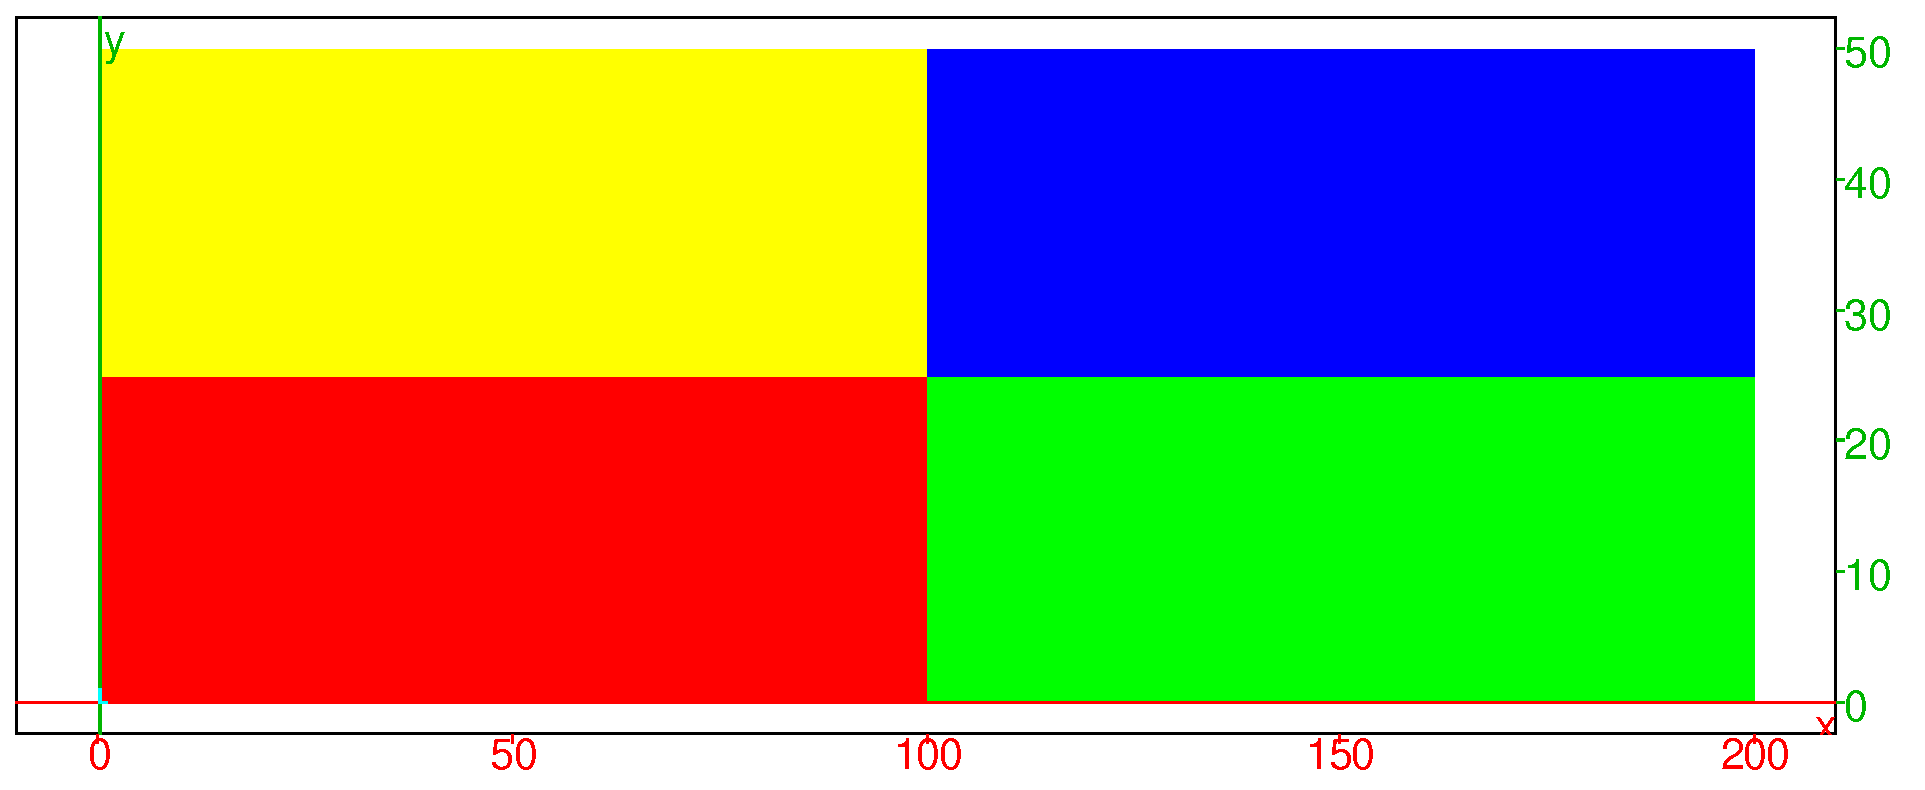
\includegraphics[width=\textwidth]{image1234}\\
On sauve  cette image (bouton {\tt M} situ\'e \`a gauche) sous le nom
{\tt image1234}, ce qui cr\`ee :\\
{\tt image1234.eps},  {\tt image1234.jpg}, {\tt image1234.png},
{\tt image1234.pdf}.
On tape :
\begin{center}{\tt a:=readrgb("image1234.jpg")}\end{center}
\begin{center}{\tt a[0]}\end{center}
On obtient : {\tt [4,363,908]}\\
Puis on tape :
\begin{center}{\tt writergb("image2134.png",[a[0],a[2],a[1],a[3],a[4]])}\end{center}
On obtient (le rouge est devenu vert et le vert est devenu rouge) :\\
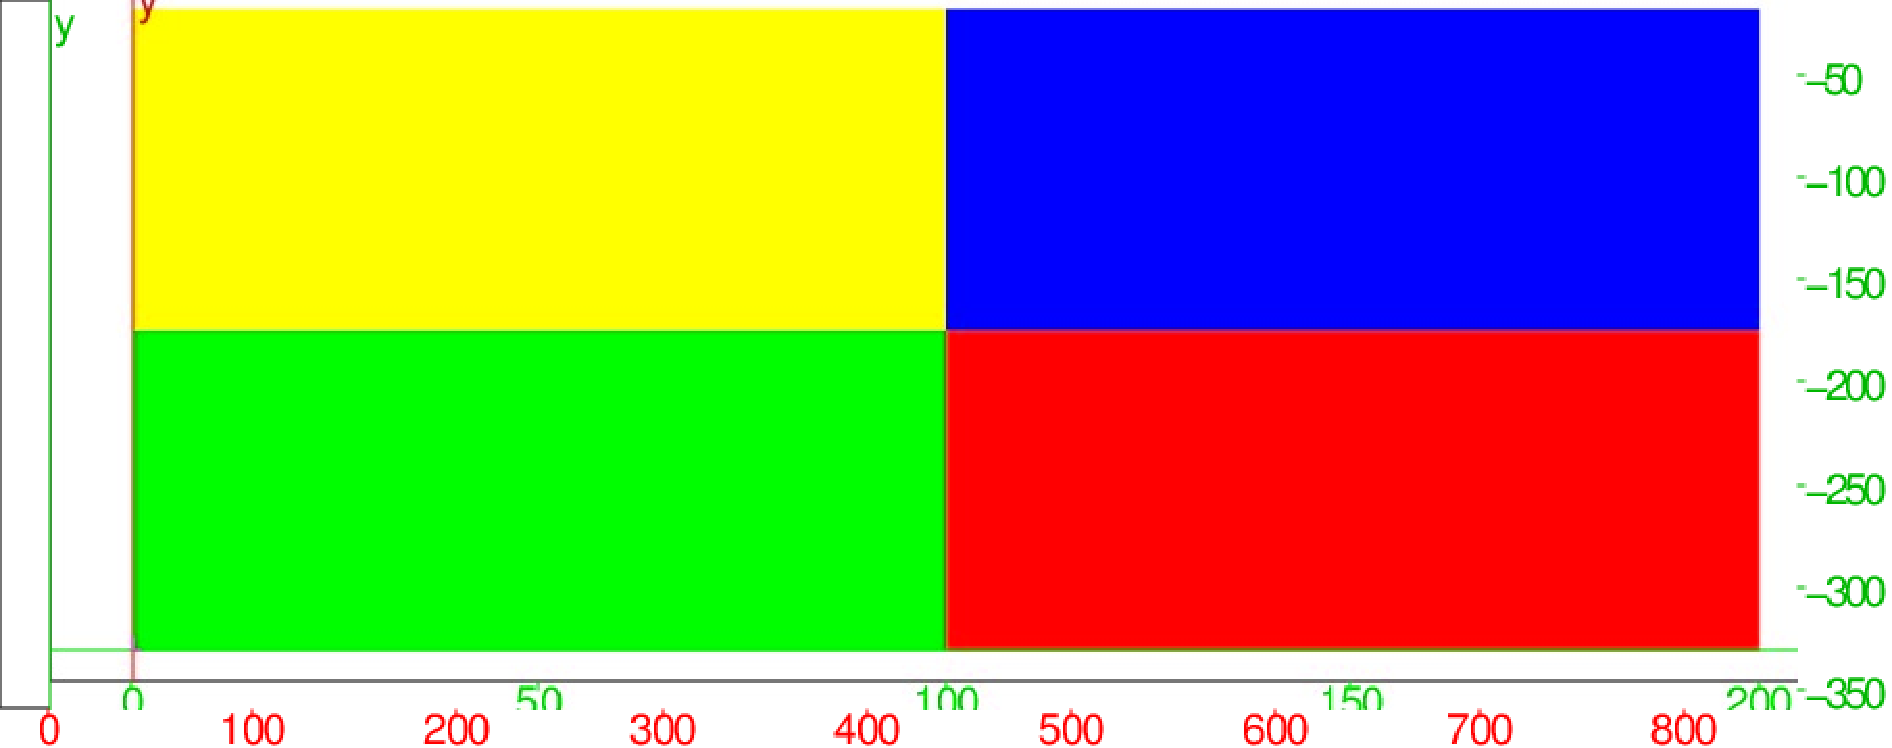
\includegraphics[width=\textwidth]{image2134}\\
Ou on tape dans un terminal :
\begin{center}{\tt gimp "image2134.png"}\end{center}
On obtient :
\begin{center}{\tt l'image de d\'epart dans laquelle le rouge est devenu vert et le vert est devenu rouge}\end{center}
Essayer de cr\`eer une image :
\begin{center}{\tt writergb("essai1.png",[[4,2,2],[[255,0],[0,0]], [[0,255],[0,0]],[[255,125],[255,255]], [[0,0],[255,0]]])}\end{center}
vous obtenez (avec un vert attenu\'e du au 125 de la 3i\`eme matrice):\\
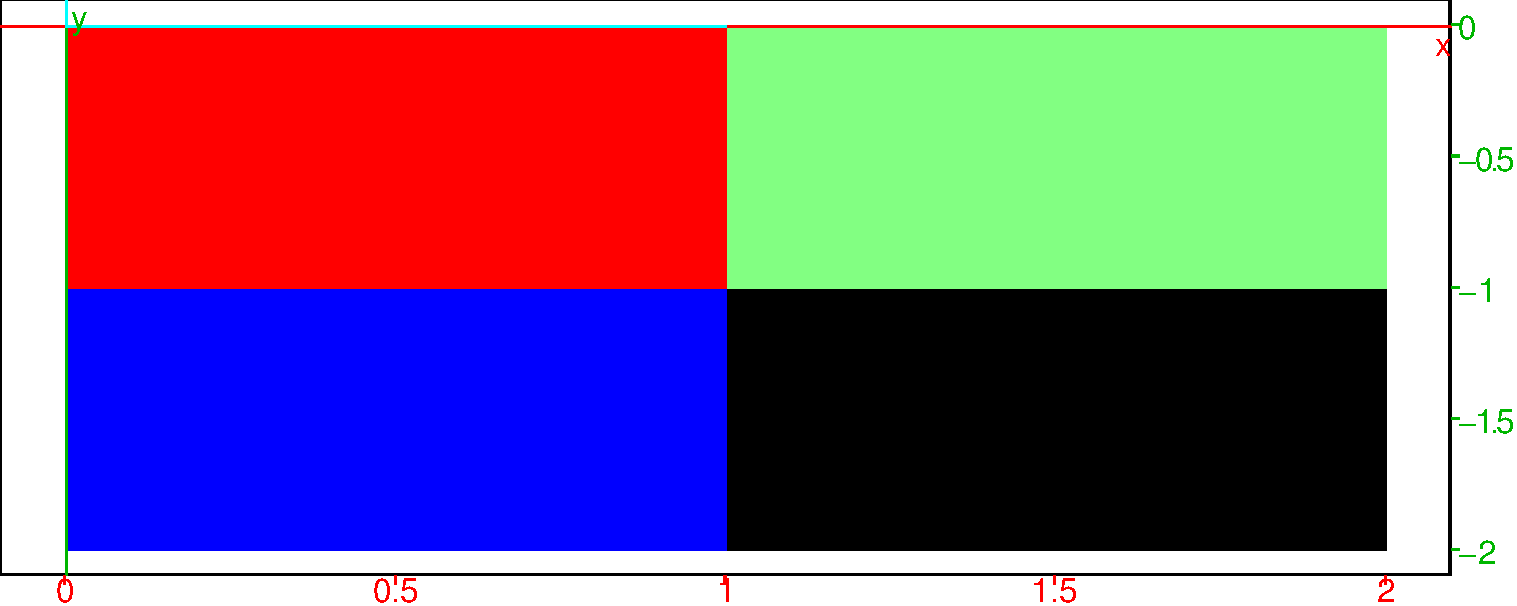
\includegraphics[width=\textwidth]{writergb1}
ou encore essayer :
\begin{center}{\tt writergb("image1.png",[[4,2,3],[[255,0,255],[0,255,0]], [[0,0,255],[0,0,0]],[[255,125,125],[255,255,255]], [[0,0,0],[255,255,0]]])}\end{center}
\item On peut aussi cr\'eer et stocker des images, au format PNG avec une
version simplifi\'ee de la syntaxe : pas d'argument correspondant au nombre
de canaux et aux dimensions de la matrice des pixels de cette image ni de
matrice correspondant \`a la transparence.\\
{\tt writergb} a alors deux ou quatre arguments : le nom du fichier dans lequel
on veut stocker la nouvelle image et la matrice des niveaux de gris des pixels,
ou 3 matrices (du rouge, du vert et du bleu) donnant la couleur RGB des
pixels.\\
Par exemple :
\begin{center}{\tt writergb("image2.png",[[65,125],[185,200]])}\end{center}
cr\'ee et affiche une image 2x2 pixels au format PNG en 4 niveaux de gris
(0 noir, 255 blanc)
\begin{center}{\tt writergb("image3.png",[[255,250],[0,120]],[[0,255],[0,0]], [[0,0],[255,100]])}\end{center}
cr\'ee et affiche une image 2x2 pixels au format PNG en RGBA avec 256 niveaux
pour chaque couleur (rouge, bleu, vert). Ici la premi\`ere ligne rouge, jaune 
(m\'elange de rouge (240) et vert (255)) et la deuxi\`eme ligne est bleu,violet (m\'elange de rouge(120) et de bleu (100)).\\
Essayez :
\begin{center}{\tt writergb("essai2.png",[[4,300,300],makemat(0,300,300), makemat(0,300,300), makemat(255,300,300), makemat(0,300,300)+idn(300)*255])}\end{center}
\begin{center}{\tt writergb("essai3.png",[[4,300,300],makemat(250,100,100)+ranm(100,100), makemat(0,100,100)+ranm(100,100), makemat(255,100,100), makemat(0,100,100)+ranm(100,100)])}\end{center}
{\bf Remarque}\\
Il y a 2 choses distinctes: le nombre de points de l'image numeris\'ee et la 
repr\'esentation graphique dans {\tt Xcas} qui se fait dans un rectangle avec 
des coordonn\'ees. Dans [4,300,100] il y a 300 points horizontalement et 100 
verticalement, si on met l'image dans un rectangle du plan, selon l'echelle 
choisie pour le graphique horizontalement et verticalement, l'image 300x100 
peut \^etre toute petite ou tr\`es grande. Si c'est tres grand chaque point de 
l'image numeris\'ee originale sera repr\'esent\'e par un petit rectangle qui 
occupera plusieurs pixels physiques sur l'\'ecran.
\end{itemize}
\section{D\'efinition des variables typ\'ees}
Soit la variable {\tt a} on peut donner sont type soit en la renommant soit en 
mettant {\tt :} puis son type :\\
{\tt a\_i} ou {\tt a:integer} pour signifier que {\tt a} est de type entier\\
{\tt a\_d} ou {\tt a:double} ou {\tt a:real} pour signifier que {\tt a} est de type r\'eel\\
{\tt a\_c} ou {\tt a:complex} pour signifier que {\tt a} est de type complexe\\
{\tt a\_v} ou {\tt a:vector} pour signifier que {\tt a} est de type vecteur\\
{\tt a\_m} ou {\tt a:matrix} pour signifier que {\tt a} est de type matrice\\
{\tt a\_s} ou {\tt a:string} pour signifier que {\tt a} est de type cha\^{\i}ne
de caract\`eres\\
\subsection{Pour traduire un programme {\tt Xcas} en $C^{++}$}\index{insmode}\index{cpp}
Lorsqu'un programme {\tt Xcas} (par exemple {\tt nomprog}) a des variables typ\'ees, on pourra le traduire en  $C^{++}$ et le compiler gr\^ace \`a la commande {\tt cpp} suivi du nom du 
programme (par exemple {\tt cpp(nomprog)})\\
Cela va cr\'eer un fichier {\tt giac\_nomprog.cpp} et un fichier 
{\tt libgiac\_nomfichier.so} sur le disque dur.\\
{\bf Attention} le nom du fichier doit avoir plus qu'une lettre.\\
Par exemple :\\
{\tt truc(n:integer):=\{return 2*n+1;\}} puis \\
{\tt  cpp(truc)}\\
On obtient :\\
{\tt 1}\\
et cela a cr\'e\'e sur le disque dur le fichier {\tt giac\_truc.cpp} qui est 
un fichier $C^{++}$ et le fichier {\tt libgiac\_truc.so} qui est 
le fichier  $C^{++}$  compil\'e :\\
Voici ce que contient {\tt giac\_truc.cpp} :
\begin{verbatim}
#include <giac/giac.h>
using namespace std;
namespace giac {
giac::gen truc(int n_i,const giac::context * contextptr){
giac::makevecteur(return 2*n_i+1)
}
giac::gen _truc(const giac::gen & g,const giac::context * contextptr){
return truc(g,contextptr);
}

const string _truc_s("truc");
unary_function_eval __truc(0,&_truc,_truc_s);
unary_function_ptr at_truc(&__truc,0,true);
}
\end{verbatim}
La commande {\tt insmode(nomprog)} utilisé dans une session {\tt Xcas} va lire
 le module compil\'e {\tt libgiac\_truc.so} sur le disque dur.\\
On peut alors utiliser le m\^eme nom {\tt nomprog}) dans cette session {\tt Xcas} 
mais le programme sera plus efficace gr\^ace \`a la compilation.

\chapter{Utilisation de  {\tt giac} \`a l'int\'erieur d'un programme}
\section{Utilisation dans un programme  {\tt C++}}
On peut utiliser {\tt giac} \`a l'int\'erieur d'un programme {\tt C++} en
mettant au d\'ebut du programme par exemple {\tt essai.cc} :\\
{\tt \#include<giac/giac.h>}\\
puis en compilant le compilant avec :\\
{\tt c++ -g essai.cc -lgiac -lgmp}\\
 et en l'ex\'ecutant en mettant :\\
{\tt ./a.out}\\
{\bf Exemple}
\begin{verbatim}
// -*- compile-command: "g++ -g pgcd.cc -lgiac -lgmp" -*-
#include <giac/giac.h>

using namespace std;
using namespace giac;

gen pgcd(gen a,gen b){
  gen q,r;
  for (;b!=0;){
    r=irem(a,b,q);
    a=b;
    b=r;
  }
  return a;
}

int main(){
  cout << "Entrer 2 entiers";
  gen a,b;
  cin >> a >> b;
  cout << pgcd(a,b) << endl;
  return 0;
} 
\end{verbatim}
\section{Pour d\'efinir de nouvelles fonctions de {\tt giac}}
On peut d\'efinir de nouvelles fonctions qui deviendront des 
fonctions de {\tt giac}. Pour d\'efinir par exemple la fonction de nom 
{\tt pgcd} ( et c'est l'instruction  : {\tt const string \_pgcd\_s("pgcd")}; qui d\'efinit le nom de la fonction), on tape :
\index{insmod}
\begin{verbatim} 
// -*- mode:C++ ; compile-command: "g++ -I.. -fPIC -DPIC 
-g -c pgcd.cpp  -o pgcd.lo && ln -sf pgcd.lo pgcd.o && gcc 
-shared pgcd.lo -lc  -Wl,-soname -Wl,libpgcd.so.0 -o 
libpgcd.so.0.0.0 &&  ln -sf libpgcd.so.0.0.0 libpgcd.so.0 && 
 ln -sf libpgcd.so.0.0.0 libpgcd.so" -*-
using namespace std;
#include <stdexcept>
#include <cmath>
#include <cstdlib>
#include <giac/giac.h>
#include "pgcd.h"

#ifndef NO_NAMESPACE_GIAC
namespace giac {
#endif // ndef NO_NAMESPACE_GIAC

  gen pgcd(gen a,gen b){
    gen q,r;
    for (;b!=0;){
      r=irem(a,b,q);
      a=b;
      b=r;
    }
    return a;
  }
  gen _pgcd(const gen & args){
    if ((args.type!=_VECT)||(args._VECTptr->size()!=2))
      setsizeerr();
    vecteur &v=*args._VECTptr;
    return pgcd(v[0],v[1]);
  }
  const string _pgcd_s("pgcd");
  unary_function_unary __pgcd(&_pgcd,_pgcd_s);
  unary_function_ptr at_pgcd (&__pgcd,0,true);
  

#ifndef NO_NAMESPACE_GIAC
} // namespace giac
#endif // ndef NO_NAMESPACE_GIAC
\end{verbatim}
On compile avec la commande situ\'ee apr\`es {\tt compile-command} de 
l'en-t\^ete du programme. Puis, pour l'ins\'erer dans 
une session {\tt Xcas}, il faut taper la commande {\tt insmod}
 suivi du chemin absolu complet de la librairie, par exemple :\\
{\tt insmod("/home/user/giac-0.4.0/doc/en/libpgcd.so")}.\\
Cela suppose que le source de giac a \'et\'e d\'esarchiv\'e dans le 
r\'epertoire /home/user).
\subsubsection{Le type {\tt gen}}
{\tt gen} est le type qui sert \`a repr\'esenter toutes les
donn\'ees de calcul formel : les fonctions de calcul formel travaillent sur des
{\tt gen}.\\
Si g est de type {\tt gen} ( {\tt gen g;}), selon le type de {\tt g},
 {\tt g.type} aura diff\'erentes valeurs qui sont :\\
{\tt \_INT\_} si {\tt g.val} est un entier de type {\tt int},\\
{\tt \_DOUBLE\_} si {\tt g.\_DOUBLE\_val} est un r\'eel de type {\tt double}\\
{\tt \_SYMB} si {\tt g.\_SYMBptr} pointe sur un objet de type {\tt symbolique}\\
{\tt \_VECT} si {\tt g.\_VECTptr} pointe sur un vecteur  de type {\tt vecteur}\\
{\tt \_ZINT} si {\tt g.\_ZINTptr} pointe sur un entier de type {\tt zint}\\
{\tt \_IDNT} si {\tt g.\_IDNTptr} pointe sur un identificateur de type {\tt idnt}\\
{\tt \_CPLX} si {\tt g.\_CPLXptr} pointe sur un complexe  de type {\tt complexe}

\end{document}

\subsection{L'affinit\'e : {\tt affinity affinite}}\index{affinite}\index{affinity}\label{sec:affinite2}
%{\bf Voir aussi :} \ref{sec:affinite3} pour la g\'eom\'etrie 3-d.\\
\noindent {\tt affinite}, en g\'eom\'etrie plane, a trois ou quatre 
param\`etres : deux droites $D1$ (l'axe), $D2$ (la direction), $k$ (le rapport)
et un point.\\
Si {\tt a:=affinite(D1,D2,k)} {\tt a} est l'affinit\'e d'axe {\tt D1}, de 
direction {\tt D2} et de rapport {\tt k}. Si {\tt N:=a(M)}, la droite {\tt MN} 
est parall\`ele \`a {\tt D2}  et rencontre {\tt D1} en {\tt J} et on a :
{\tt $\overrightarrow{JN}$=k* $\overrightarrow{JM}$}.\\
On tape :
\begin{center}{\tt a:=affinite(droite(0,1),droite(-1,i),2)}\end{center}
Puis :
\begin{center}{\tt a(1+i)}\end{center}
On obtient :
\begin{center}{\tt Le point 2+2*i trac\'e avec une croix (x) noire}\end{center}
Si {\tt A1:=affinite(D1,D2,k,A)} {\tt A1} est le transform\'e de {\tt A} dans
 l'affinit\'e d'axe {\tt D1}, de direction {\tt D2} et de rapport {\tt k}. Si
$P$ est le point d'intersection de $D1$ avec la parall\'ele \`a $D2$ 
passant par $A$, on a alors $\overrightarrow{PA1}=k\overrightarrow{PA}$.\\
On tape :
\begin{center}{\tt affinite(droite(0,1),droite(-1,i),2,1+i)}\end{center}
On obtient :
\begin{center}{\tt Le point 2+2*i trac\'e avec une croix (x) noire}\end{center}
%\subsection{L'affinit\'e : {\tt affinite}}\index{affinite}\label{sec:affinite3}{\bf Voir aussi :} \ref{sec:affinite2} pour la g\'eom\'etrie plane.\\\noindent {\tt affinite}, en g\'eom\'etrie 3-d, a trois ou quatre param\`etres~:un plan $D1$ (l'axe), $D2$ (la direction), $k$ (le rapport) et un point.\\Si {\tt a:=affinite(D1,D2,k)} {\tt a} est l'affinit\'e d'axe {\tt D1}, de direction {\tt D2} et de rapport {\tt k}.\\
\subsection{Pour les habitu\'es de {\tt Xcas}}
La nouvelle interface {\tt Xcas} est plus facile d'acc\`es que l'interface
{\tt Xcas} car les diff\'erents \'ecrans sont visibles les uns \`a la suite 
des autres.\\
Il faut savoir que :
\begin{itemize}
\item l'\'ecran {\tt hist io} de {\tt Xcas} qui servait \`a 
l'\'ecriture des r\'esultats interm\'ediaires d'un programme est remplac\'e 
par un emplacement situ\'e entre la commande et le r\'esultat et o\`u les 
r\'esultats interm\'ediaires seront \'ecrits en bleu. Bien s\^ur lorsqu'il n'y
a pas de r\'esultats interm\'ediaires, cet emplacement n'est pas visible.\\
On tape par exemple :\\
{\tt for (j:=1;j<5;j++) \{print(3*j);\}} \\
On obtient :\\
{\tt 3\\6\\9\\12}\\
\'ecrit en bleu dans la zone des r\'esultats interm\'ediaires et,\\
{\tt 1}\\
 \'ecrit en noir dans la zone pour la r\'eponse car l'instruction 
{\tt print} renvoie {\tt 1}. 
\item l'\'ecran {\tt geo io} de {\tt Xcas} qui servait aux sorties graphiques
interm\'ediaires d'un programme est remplac\'e par un \'ecran que l'on obtient
\`a l'aide du menu {\tt Cfg} puis {\tt Montrer} puis {\tt DispG}.\\
Par exemple, les dessins r\'ecursifs ne seront visibles que dans cet \'ecran.
On ne peut pas avoir plusieurs \'ecrans de ce type et donc cet \'ecran 
refl\`ete toutes les sorties graphiques de la session. On peut l'effacer : 
l'instruction {\tt ClrGraph()} tap\'ee depuis une ligne de commandes de la 
session efface cet \'ecran.
\end{itemize}
Il faut savoir que :
les boutons rouges {\tt cas geo gen} qui servaient \`a ouvrir des fen\^etres 
permettant de r\'egler les diff\'erentes configurations, sont remplac\'es par :
\begin{itemize}
\item le bouton donnant la ligne d'\'etat ou le  menu 
{\tt Cfg$\blacktriangleright$Configuration du CAS},
\item le menu {\tt Cfg$\blacktriangleright$Configuration graphique},
\item le menu {\tt Cfg$\blacktriangleright$Configuration generale}. 
\end{itemize}
Il faut savoir que :
les boutons jaunes {\tt eqw geo hist mtrw prg} qui servaient \`a ouvrir des
fen\^etres permettant d'avoir diff\'erents \'ecrans, sont remplac\'es par :
\begin{itemize}
\item {\tt Alt+e} pour ouvrir une nouvelle entr\'ee de type \'editeur 
d'\'equation,
\item {\tt Alt+g} pour ouvrir une nouvelle entr\'ee de type \'ecran de 
g\'eom\'etrie plane,
\item {\tt Alt+n} pour ouvrir une nouvelle entr\'ee de type ligne de 
commandes,
\item {\tt Alt+t} pour ouvrir  une nouvelle entr\'ee de type tableur,
\item {\tt Alt+p} pour ouvrir  une nouvelle entr\'ee de type \'editeur de 
programmes.
\end{itemize}
On a en plus, la possibilit\'e d'avoir deux nouveaux \'ecrans avec :
\begin{itemize}
\item {\tt Alt+d} pour ouvrir une nouvelle entr\'ee de type \'ecran de 
g\'eom\'etrie tortue,
\item {\tt Alt+h} pour ouvrir une nouvelle entr\'ee de type \'ecran de 
g\'eom\'etrie 3-d.
\end{itemize}

ou on utilise le menu 
{\tt Edit$\blacktriangleright$Ajouter$\blacktriangleright$equation} de la 
session \`a la place des raccourcis clavier {\tt Alt+e} etc...

\subsection{Pour un script}\label{sec:script}
On peut ex\'ecuter un script pas \`a pas, si il se trouve dans la
{\tt Fen\^etre de script}. Cette fen\^etre est visible en utilisant le menu :\\
{\tt Session$\blacktriangleright$Montrer$\blacktriangleright$Montrer la fenetre de script}.\\
On peut recopier le script dans cette fen\^etre, avec la souris, depuis un 
\'editeur de programmes ou bien charger le fichier contenant le script avec 
le menu {\tt Fich$\blacktriangleright$Charger} de cette fen\^etre. Pour
ex\'ecuter le script ligne par ligne, on clique sur la ligne \`a ex\'ecuter, 
puis, sur la ligne de commandes o\`u on veut que cela s'ex\'ecute, puis, on 
clique sur le bouton {\tt exec} : le script s'ex\'ecute alors ligne par ligne.
{\bf Attention} \\
Il ne faut rien faire entre, cliquer sur la ligne \`a ex\'ecuter et choisir
la ligne de commandes. De plus, cette ligne de commandes doit se trouver \`a 
la fin de votre session, ou \`a la 
fin des lignes de commandes d'un \'ecran graphique ou tortue, pour que de
nouvelles lignes soient cr\'e\'ees automatiquement au fur et \`a mesure de 
l'ex\'ecution du script.

on s\'electionne cette colonne, il nous reste \`a d\'eterminer la
colonne sortant de la matrice identit\'e, c'est-\`a-dire la ligne
du pivot utilis\'e~:
\begin{itemize} 
\item tout d'abord la coordonn\'ee positive du sommet
en colonne sortante 
va \^etre ramen\'e \`a 0, et cela doit compenser l'augmentation
de 0 \`a une valeur positive de la coordonn\'ee en une
colonne entrante, donc dans la colonne entrante, ligne
sortante, le coefficient dans la matrice doit \^etre strictement positif,
\item  d'autre part les autres coefficients du sommet doivent rester
  positifs. Pour r\'ealiser cela, on calcule de la ligne 1 \`a $m$
les rapport des coefficients de cette ligne derni\`ere colonne avec
le coefficient de cette ligne, colonne sortante,
en cherchant la ligne qui donne un rapport positif le plus petit
possible.
S'il n'existe pas de telle ligne, le maximum est alors
$+\infty$ (car on peut ind\'efiniment augmenter la valeur de la
composante ayant ce num\'ero de colonne en restant dans le domaine). 
Si une telle ligne existe, on se sert du coefficient
de cette ligne/colonne comme d'un pivot, et on cr\'ee un 1 \`a cette
ligne et des 0 ailleurs dans
cette colonne par combinaisons lin\'eaires de lignes.
\end{itemize}
plotode([-y,-1+x^2+y^2], [t=-3..3,x,y],[0,1,0.1],plan)
plotode([-y,-1+x^2+y^2], [t=-3..3,x,y],[0,1,0.5],plan)
plotode([-y,-1+x^2+y^2], [t=-6..3.65,x,y],[0,0.828,0.828],plan)
plotode([-y,-1+x^2+y^2], [t=-1.2..1.2,x,y],[0,-1.2,0],plan)
poisson(a):={
local L;
L:=NULL;
L:=L,plotode([-y+a,-1+(x-a)^2+(y-a)^2], [t=-3..3,x,y],[0,a+1,a+0.1],plan);
L:=L,plotode([-y+a,-1+(x-a)^2+(y-a)^2-y,-1+x^2+y^2], [t=-3..3,x,y],[0,a+1,a+0.5],plan);
L:=L,plotode([-y+a,-1+(x-a)^2+(y-a)^2], [t=-6..3.65,x,y],[0,a+0.827,a+0.827],plan);
L:=L,plotode([-y+a,-1+(x-a)^2+(y-a)^2], [t=-1.3..1.3,x,y],[0,a-1.1,a],plan);
return L;}


\subsection{Test de primalit\'e : {\tt is\_prime isprime isPrime}}\index{is\_prime}\index{isprime}\index{isPrime}\index{pari}
\noindent {\tt is\_prime(n)}  renvoie {\tt 1} (vrai) ou {\tt 0} (faux)
selon que son argument est premier ou non. {\tt isprime} ou {\tt isPrime} renvoie {\tt true}
ou {\tt false}. Utiliser la commande  {\tt is\_prime(n,1)} (ou {\tt pari("isprime",n,1)})
pour obtenir un certificat de primalit\'e (voir la documentation
de PARI/GP, depuis le menu {\tt Aide->Manuels->PARI-GP)}) et
{\tt pari("isprime",n,2)} ou {\tt is\_prime(n,2)} pour utiliser le test APRCL.

On tape :
\begin{center}{\tt is\_prime(100003)}\end{center}
On obtient :
\begin{center}{\tt 1}\end{center}
On tape :
\begin{center}{\tt isprime(100003)}\end{center}
On obtient :
\begin{center}{\tt true}\end{center}
On tape :
\begin{center}{\tt is\_prime(98569898989987)}\end{center}
On obtient :
\begin{center}{\tt 1}\end{center}
On tape :
\begin{center}{\tt is\_prime(14)}\end{center}
On obtient :
\begin{center}{\tt 0}\end{center}
On tape :
\begin{center}{\tt isprime(14)}\end{center}
On obtient :
\begin{center}{\tt false}\end{center}
Pour obtenir un certificat de primalit\'e pour $n=9856989898997789789$,
on tape :
\begin{center}{\tt isprime(9856989898997789789,1)}\end{center}
ou~:
\begin{center}{\tt pari("isprime",9856989898997789789,1)}\end{center}
On obtient les coefficients prouvant la primalit\'e par le test
"p-1" de Selfridge-Pocklington-Lehmer~:
\begin{center}
{\tt [[2,2,1],[19,2,1],[941,2,1],[1873,2,1],[94907,2,1]]}
\end{center}
sinon, on tape :
\begin{center}{\tt pari("isprime",9856989898997789789,2)}\end{center}
Ou on tape :
\begin{center}{\tt is\_prime(9856989898997789789)}\end{center}
On obtient :
\begin{center}{\tt 1}\end{center}

Sur un corps K « valu\'e » (au sens : muni d'une valeur absolue) et non discret 
(typiquement : K = R ou C), soient E et F deux espaces vectoriels norm\'es respectivement munis des normes ‖ ‖1 et ‖ ‖2.

Soit f une application lin\'eaire de E dans F. Consid\'erons $N:=\sup _{{v\neq 0}}{\frac {\|f(v)\|_{2}}{\|v\|_{1}}}$.

Si N < +∞, on dit que N est la norme de l'op\'erateur f, subordonn\'ee \`a $\| \|_1$ et $\| \|_2$

{\bf Propri\'et\'es}

    N est fini si et seulement s'il existe des r\'eels C tels que, pour tout v ∈ E, ‖f(v)‖2 ≤ C‖v‖1 (autrement dit : tels que f soit C-lipschitzienne), et dans ce cas N est \'egal au plus petit d'entre ces r\'eels C.
    Si N est fini alors f est N-lipschitzienne et par cons\'equent uniform\'ement continue, donc continue, donc continue en 0. R\'eciproquement, si f est continue en 0, alors N est fini (la preuve, classique pour K = R ou C, se g\'en\'eralise).
    N est fini si et seulement si l'image par f de toute partie born\'ee de E (ou simplement : de la boule unit\'e) est born\'ee. Ceci explique le nom d'op\'erateurs born\'es \'egalement donn\'e aux applications lin\'eaires continues de E dans F.
    Dans l'espace L(E,F) des applications lin\'eaires de E dans F, le sous-espace {\mathcal L}(E,F) de celles qui sont continues peut donc être muni de la norme subordonn\'ee. Alors, l'application bilin\'eaire :\\
${\mathcal L}(E,F)\times E\to F,(f,v)\mapsto f(v)$ est continue.\\
    Si E est de dimension finie, toute application lin\'eaire de E dans F est 
continue : $L(E,F)={\mathcal L}(E,F)$.\\
    Si K = R ou C, N est aussi \'egal \`a :\\
$\sup _{{\|v\|_{1}=1}}\|f(v)\|_{2}=\sup _{{\|v\|_{1}\leqslant 1}}{\frac {\|f(v)\|_{2}}{\|v\|_{1}}}$.

\subsection{Norme $l^\infty$ d'une matrice : {\tt maxnorm}}\index{maxnorm}\label{sec:maxnormm}
\noindent{\tt maxnorm} a comme argument une matrice $A$ (voir aussi \ref{sec:maxnormv}).\\
{\tt maxnorm} renvoie $\max(|a_{j,k}|)$ si l'argument est $A=a_{j,k}$.\\
On tape :
\begin{center}{\tt maxnorm([[1,2],[3,-4]])}\end{center}
On obtient :
\begin{center}{\tt 4}\end{center}
En effet : $\max(|a_{j,k}|)=4$

\section{Comment lire et cr\'eer une image}
\subsection{Qu'est-ce qu'une image ?}
Pour {\tt Xcas} une image est une liste {\tt a} de 5 \'el\'ements :
\begin{itemize}
\item {\tt a[0]} est une liste de 3 \'el\'ements : le nombre de canaux (3 ou 4)
et le nombre de lignes $n$ et de colonnes $p$ utilis\'es pour la dimension de 
l'image,
\item {\tt a[1]} correspond au canal rouge : c'est une matrice $n,p$ de nombres
entiers entre 0 et 255,
\item {\tt a[2]} correspond au canal vert : c'est une matrice $n,p$ de nombres
entiers entre 0 et 255,
\item {\tt a[3]} correspond au canal pour la transparence : c'est une matrice 
$n,p$ de nombres entiers entre 0 et 255,
\item {\tt a[4]} correspond au canal bleu : c'est une matrice $n,p$ de nombres
entiers entre 0 et 255,
\end{itemize}

\subsection{Pour lire une image : {\tt readrgb}}\index{readrgb}
\noindent{\tt readrgb} peut lire un fichier contenant une image. Ce fichier 
peut \^etre un fichier {\tt .jpg} ou {\tt .png} ou {\tt .gif}.\\
{\tt readrgb} renvoie [[nombre\_canaux,largeur,hauteur],rouge,vert,transparence,bleu] o\`u rouge,vert,transparence,bleu sont des matrices.\\ 
On tape :
\begin{center}{\tt a:=readrgb("image.jpg")}\end{center}
On obtient :
\begin{center}{\tt une liste de 5 \'el\'ements qui sont [4,20,10] suivi de 4 matrices de dimension 20,10 qui indiquent o\`u sont situ\'e les couleurs rouge,vert,transparence,bleu]}\end{center}

\subsection{Pour  recr\'eer ou cr\'eer une image : {\tt writergb}}\index{writergb}
\noindent{\tt writergb} permet de stocker une image lue avec {\tt readrgb} dans
un fichier de suffixe {\tt .png}.\\
ou \\ 
de cr\'eer une image et de la stocker dans un fichier de suffixe {\tt .png}.
On peut cr\'eer cette image avec des niveaux de gris ou des 
niveaux des  diff\'erentes couleurs. 
\begin{itemize}
\item On poss\'ede une variable (par exemple {\tt a}) contenant une image lue 
avec {\tt readrgb}. \\
{\tt writergb} a deux arguments : le nom du fichier dans lequel on veut stocker 
la nouvelle image et une liste contenant {\tt a[0]} (liste contenant le nombre 
de canaux et les dimensions de la matrice des pixels de cette image), puis les 
couleurs de cette image qui sont les matrices {\tt a[1]} pour la couleur rouge,
{\tt a[2]} pour la couleur verte, {\tt a[3]} pour la transparence et {\tt a[4]}
pour la couleur bleu.\\
La transparence permet de superposer plusieurs images : sa valeur va de 0 \`a 
255 (si la transparence vaut 0 c'est un cache !).\\
On tape :
\begin{center}{\tt a:=readrgb("image.jpg")}\end{center}
Puis on tape :
\begin{center}{\tt writergb("imagevrb.png",[a[0],a[2],a[1],a[3],a[4]])}\end{center}
Puis on tape :
\begin{center}{\tt gimp "imagevrb.png"}\end{center}
On obtient :
\begin{center}{\tt l'image de d\'epart dans laquelle le rouge est devenu vert et le vert est devenu rouge}\end{center}
Essayer de cr\`eer une image :
\begin{center}{\tt writergb("essai.png",[[4,2,2],[[255,0],[0,0]], [[0,255],[0,0]],[[255,125],[255,255]], [[0,0],[255,0]]])}\end{center}
vous obtenez (avec un vert attenu\'e du au 125 de la 3i\`eme matrice):\\
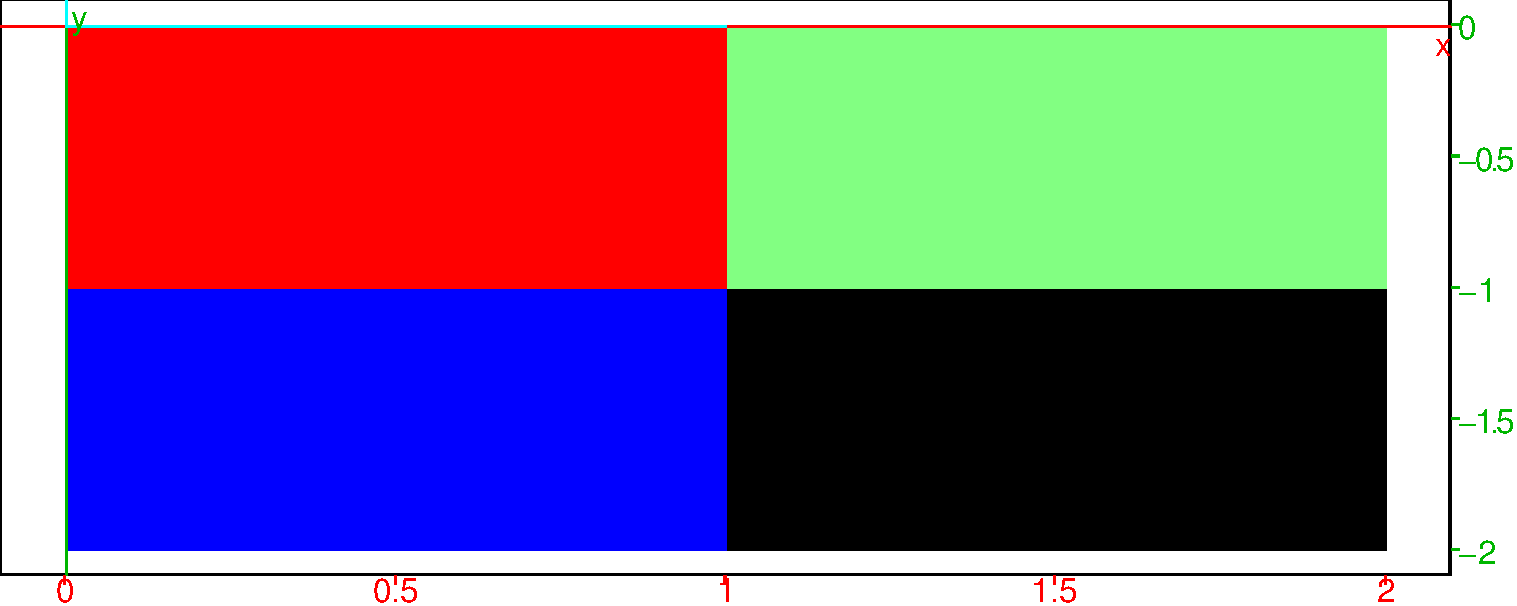
\includegraphics[width=\textwidth]{writergb1}
ou encore essayer :\\
\begin{center}{\tt writergb("image1.png",[[4,2,3],[[255,0,255],[0,255,0]], [[0,0,255],[0,0,0]],[[255,125,125],[255,255,255]], [[0,0,0],[255,255,0]]])}\end{center}
\item On peut aussi cr\'eer et stocker des images, au format PNG avec une 
version simplifi\'ee de la syntaxe : pas d'argument correspondant au nombre 
de canaux et aux dimensions de la matrice des pixels de cette image ni de 
matrice correspondant \`a la transparence.\\
{\tt writergb} a alors deux ou quatre arguments : le nom du fichier dans lequel
on veut stocker la nouvelle image et la matrice des niveaux de gris des pixels,
ou 3 matrices (du rouge, du vert et du bleu) donnant la couleur RGB des 
pixels.\\
Par exemple :\\
\begin{center}{\tt writergb("image.png",[[255,0],[0,255]])}\end{center}
cr\'ee et affiche une image 2x2 pixels au format PNG en 256 niveaux de gris 
(0 noir, 255 blanc)
\begin{center}{\tt writergb("image.png",[[255,0],[0,0]],[[0,255],[0,0]], [[0,0],[255,0]])}\end{center}
cr\'ee et affiche une image 2x2 pixels au format PNG en RGBA avec 256 niveaux 
pour chaque couleur (rouge, bleu, vert). Ici la premi\`ere ligne rouge,vert et la deuxi\`eme ligne est bleu,noir.
Essayez :
\begin{center}{\tt writergb("essai3.png",[[4,300,300],makemat(0,300,300), makemat(0,300,300), makemat(255,300,300), makemat(0,300,300)+idn(300)*255])}\end{center}
et
\begin{center}{\tt writergb("essai4.png",[[4,300,300],makemat(250,100,100)+ranm(100,100), makemat(0,100,100)+ranm(100,100), makemat(255,100,100), makemat(0,100,100)+ranm(100,100)])}\end{center}
\end{itemize}
